% !TEX program = xelatex
\documentclass[UTF8,fontset=fandol,a4paper,11pt]{ctexart}
\usepackage[margin=21mm,top=23mm,bottom=22mm,headheight=16pt]{geometry}
\usepackage{amsmath,amssymb,mathtools,bm}
\usepackage{tikz}
\usetikzlibrary{arrows.meta,calc,angles,quotes,patterns,decorations.pathmorphing}
\usepackage{xcolor,booktabs,array,longtable,enumitem,fancyhdr,needspace}
\usepackage[unicode,hidelinks]{hyperref}
\definecolor{ink}{HTML}{24343C}
\definecolor{accent}{HTML}{166A70}
\definecolor{muted}{HTML}{65747A}
\definecolor{rulegray}{HTML}{D4DDE0}
\definecolor{warm}{HTML}{966037}
\color{ink}
\setlength{\parindent}{2em}
\setlength{\parskip}{4pt}
\linespread{1.12}
\AtBeginDocument{\setlength{\abovedisplayskip}{6pt plus 2pt minus 1pt}
\setlength{\belowdisplayskip}{6pt plus 2pt minus 1pt}
\setlength{\abovedisplayshortskip}{0pt plus 1pt}
\setlength{\belowdisplayshortskip}{4pt plus 1pt}}
\setlist[enumerate]{label=(\arabic*),leftmargin=2.3em,itemsep=3pt,topsep=4pt}
\setlist[itemize]{leftmargin=2em,itemsep=2pt,topsep=4pt}
\allowdisplaybreaks[1]
\setlength{\emergencystretch}{2em}
\setcounter{secnumdepth}{0}
\providecommand{\tightlist}{\setlength{\itemsep}{0pt}\setlength{\parskip}{0pt}}
\ctexset{section={format=\Large\bfseries\color{accent},beforeskip=10pt,afterskip=9pt},
subsection={format=\normalsize\bfseries\color{accent},beforeskip=10pt,afterskip=4pt},
subsubsection={format=\normalsize\bfseries,beforeskip=8pt,afterskip=3pt}}
\pagestyle{fancy}
\fancyhf{}
\fancyhead[L]{\small\color{muted}物理学难题集萃}
% 页眉仅保留书名；版本名称只在封面显示。
\fancyfoot[L]{\small\color{muted}\chapterlabel}
\fancyfoot[R]{\small\thepage}
\renewcommand{\headrulewidth}{0.4pt}
\renewcommand{\footrulewidth}{0pt}
\newcommand{\dd}{\mathop{}\!\mathrm{d}}
\newcommand{\vect}[1]{\bm{#1}}
\newcommand{\tagline}[1]{\noindent{\small\color{muted}#1}\par}
\newcommand{\result}[1]{\begin{equation*}\boxed{#1}\end{equation*}}
\newcommand{\figcaption}[1]{\par\vspace{2pt}{\small\color{muted}#1}\par}
\newcommand{\teach}[2]{\Needspace{4\baselineskip}\subsection*{讲解要点与追问}#1\par\smallskip\noindent\textbf{追问：}#2\par}
\newcommand{\workarea}{\par\vspace{7mm}\noindent{\small\color{muted}作答区}\par\vspace{4mm}
\noindent\textcolor{rulegray}{\rule{\linewidth}{0.3pt}}\par\vspace{16mm}
\noindent\textcolor{rulegray}{\rule{\linewidth}{0.3pt}}\par\vspace{16mm}
\noindent\textcolor{rulegray}{\rule{\linewidth}{0.3pt}}\par\vspace{16mm}
\noindent\textcolor{rulegray}{\rule{\linewidth}{0.3pt}}}
\tikzset{axis/.style={-{Stealth[length=2mm]},thin,color=muted},
motion/.style={-{Stealth[length=2.3mm]},thick,color=accent},
force/.style={-{Stealth[length=2.3mm]},thick,color=warm},
traj/.style={thick,color=accent},guide/.style={dashed,thin,color=muted},
object/.style={thick,color=ink},every node/.style={font=\small}}

\newcommand{\edition}{学生版}
\newcommand{\chapterlabel}{第一章\quad 运动学}


\providecommand{\chapterlabel}{}
\providecommand{\dd}{}
\providecommand{\edition}{}
\providecommand{\figcaption}{}
\providecommand{\footrulewidth}{}
\providecommand{\headrulewidth}{}
\providecommand{\result}{}
\providecommand{\shortworkarea}{}
\providecommand{\tagline}{}
\providecommand{\teach}{}
\providecommand{\vect}{}
\providecommand{\workarea}{}
\renewcommand{\chapterlabel}{全书目录}
\hypersetup{pdftitle={物理学难题集萃·学生版},pdfauthor={},pdfsubject={力学、热学、电磁学、光学、近代物理与试题},pdfkeywords={物理竞赛},bookmarksopen=false}


\begin{document}
\pdfbookmark[0]{物理学难题集萃}{book-cover}
\thispagestyle{empty}\vspace*{28mm}
\noindent{\Huge\bfseries 物理学难题集萃}\par\vspace{16mm}
\noindent{\LARGE\color{accent}学生版}\par\vspace{12mm}
\noindent\textcolor{accent}{\rule{\linewidth}{1pt}}\par\vspace{12mm}
\noindent 力学、热学、电磁学、光学、近代物理\par\vspace{5mm}
\noindent 分科试题与综合试题\par\vspace{10mm}
\noindent 667题\par\vfill\clearpage
\pdfbookmark[0]{全书目录}{book-contents}
\section*{全书目录}
\begin{longtable}{@{}p{124mm} r r@{}}
\toprule 章节 & 题数 & 页码\\\midrule\endfirsthead
\toprule 章节 & 题数 & 页码\\\midrule\endhead
\bottomrule\endfoot
\addlinespace[5pt]\multicolumn{3}{@{}l@{}}{\bfseries\color{accent}力学}\\
\hyperref[book-unit-1]{第一章 运动学} & 15 & \pageref{book-unit-1}\\
\hyperref[book-unit-2]{第二章 牛顿运动定律} & 20 & \pageref{book-unit-2}\\
\hyperref[book-unit-3]{第三章 功、能和动量} & 39 & \pageref{book-unit-3}\\
\hyperref[book-unit-4]{第四章 角动量与有心运动} & 14 & \pageref{book-unit-4}\\
\hyperref[book-unit-5]{第五章 静力平衡} & 12 & \pageref{book-unit-5}\\
\hyperref[book-unit-6]{第六章 刚体动力学} & 27 & \pageref{book-unit-6}\\
\hyperref[book-unit-7]{第七章 振动与波动} & 43 & \pageref{book-unit-7}\\
\addlinespace[5pt]\multicolumn{3}{@{}l@{}}{\bfseries\color{accent}热学}\\
\hyperref[book-unit-8]{热学第一章 平衡态与理想气体状态方程} & 16 & \pageref{book-unit-8}\\
\hyperref[book-unit-9]{热学第二章 热力学第一、第二定律} & 25 & \pageref{book-unit-9}\\
\hyperref[book-unit-10]{热学第三章 气体动理论} & 30 & \pageref{book-unit-10}\\
\hyperref[book-unit-11]{热学第四章 实际气体、液体、固体与相变} & 17 & \pageref{book-unit-11}\\
\addlinespace[5pt]\multicolumn{3}{@{}l@{}}{\bfseries\color{accent}电磁学}\\
\hyperref[book-unit-12]{电磁学第一章 静电场、导体与介质} & 46 & \pageref{book-unit-12}\\
\hyperref[book-unit-13]{电磁学第二章 磁场、磁介质} & 27 & \pageref{book-unit-13}\\
\hyperref[book-unit-14]{电磁学第三章 电磁感应} & 22 & \pageref{book-unit-14}\\
\hyperref[book-unit-15]{电磁学第四章 电流、直流电路} & 35 & \pageref{book-unit-15}\\
\hyperref[book-unit-16]{电磁学第五章 交流电路、暂态过程及其他} & 20 & \pageref{book-unit-16}\\
\addlinespace[5pt]\multicolumn{3}{@{}l@{}}{\bfseries\color{accent}光学}\\
\hyperref[book-unit-17]{光学第一章 几何光学} & 42 & \pageref{book-unit-17}\\
\hyperref[book-unit-18]{光学第二章 光的干涉} & 27 & \pageref{book-unit-18}\\
\hyperref[book-unit-19]{光学第三章 光的衍射} & 22 & \pageref{book-unit-19}\\
\hyperref[book-unit-20]{光学第四章 光的偏振} & 35 & \pageref{book-unit-20}\\
\hyperref[book-unit-21]{光学第五章 光的色散、散射和吸收} & 11 & \pageref{book-unit-21}\\
\addlinespace[5pt]\multicolumn{3}{@{}l@{}}{\bfseries\color{accent}近代物理}\\
\hyperref[book-unit-22]{近代物理第一章 量子物理} & 20 & \pageref{book-unit-22}\\
\hyperref[book-unit-23]{近代物理第二章 狭义相对论} & 19 & \pageref{book-unit-23}\\
\addlinespace[5pt]\multicolumn{3}{@{}l@{}}{\bfseries\color{accent}试题}\\
\hyperref[book-unit-24]{力学试题一 力学试题（一）} & 6 & \pageref{book-unit-24}\\
\hyperref[book-unit-25]{力学试题二 力学试题（二）} & 6 & \pageref{book-unit-25}\\
\hyperref[book-unit-26]{热学试题（一）} & 5 & \pageref{book-unit-26}\\
\hyperref[book-unit-27]{热学试题（二）} & 5 & \pageref{book-unit-27}\\
\hyperref[book-unit-28]{电磁学试题（一）} & 5 & \pageref{book-unit-28}\\
\hyperref[book-unit-29]{电磁学试题（二）} & 5 & \pageref{book-unit-29}\\
\hyperref[book-unit-30]{电磁学试题（三）} & 5 & \pageref{book-unit-30}\\
\hyperref[book-unit-31]{电磁学试题（四）} & 5 & \pageref{book-unit-31}\\
\hyperref[book-unit-32]{光学试题} & 6 & \pageref{book-unit-32}\\
\hyperref[book-unit-33]{近代物理试题} & 5 & \pageref{book-unit-33}\\
\hyperref[book-unit-34]{综合试题（一）} & 6 & \pageref{book-unit-34}\\
\hyperref[book-unit-35]{综合试题（二）} & 6 & \pageref{book-unit-35}\\
\hyperref[book-unit-36]{综合试题（三）} & 6 & \pageref{book-unit-36}\\
\hyperref[book-unit-37]{综合试题（四）} & 6 & \pageref{book-unit-37}\\
\hyperref[book-unit-38]{综合试题（五）} & 6 & \pageref{book-unit-38}\\
\end{longtable}\clearpage


\clearpage
\pdfbookmark[0]{力学}{subject-1}
\begingroup
\definecolor{ink}{HTML}{24343C}
\definecolor{accent}{HTML}{166A70}
\definecolor{muted}{HTML}{65747A}
\definecolor{rulegray}{HTML}{D4DDE0}
\definecolor{warm}{HTML}{966037}
\color{ink}
\setlength{\parindent}{2em}
\setlength{\parskip}{4pt}
\linespread{1.12}
\setlength{\abovedisplayskip}{6pt plus 2pt minus 1pt}
\setlength{\belowdisplayskip}{6pt plus 2pt minus 1pt}
\setlength{\abovedisplayshortskip}{0pt plus 1pt}
\setlength{\belowdisplayshortskip}{4pt plus 1pt}
\setlist[enumerate]{label=(\arabic*),leftmargin=2.3em,itemsep=3pt,topsep=4pt}
\setlist[itemize]{leftmargin=2em,itemsep=2pt,topsep=4pt}
\allowdisplaybreaks[1]
\setlength{\emergencystretch}{2em}
\setcounter{secnumdepth}{0}
\providecommand{\tightlist}{\setlength{\itemsep}{0pt}\setlength{\parskip}{0pt}}
\ctexset{section={format=\Large\bfseries\color{accent},beforeskip=10pt,afterskip=9pt},
subsection={format=\normalsize\bfseries\color{accent},beforeskip=10pt,afterskip=4pt},
subsubsection={format=\normalsize\bfseries,beforeskip=8pt,afterskip=3pt}}
\pagestyle{fancy}
\fancyhf{}
\fancyhead[L]{\small\color{muted}物理学难题集萃}
% 页眉仅保留书名；版本名称只在封面显示。
\fancyfoot[L]{\small\color{muted}\chapterlabel}
\fancyfoot[R]{\small\thepage}
\renewcommand{\headrulewidth}{0.4pt}
\renewcommand{\footrulewidth}{0pt}
\renewcommand{\dd}{\mathop{}\!\mathrm{d}}
\renewcommand{\vect}[1]{\bm{#1}}
\renewcommand{\tagline}[1]{\noindent{\small\color{muted}#1}\par}
\renewcommand{\result}[1]{\begin{equation*}\boxed{#1}\end{equation*}}
\renewcommand{\figcaption}[1]{\par\vspace{2pt}{\small\color{muted}#1}\par}
\renewcommand{\teach}[2]{\Needspace{4\baselineskip}\subsection*{讲解要点与追问}#1\par\smallskip\noindent\textbf{追问：}#2\par}
\renewcommand{\workarea}{\par\vspace{7mm}\noindent{\small\color{muted}作答区}\par\vspace{4mm}
\noindent\textcolor{rulegray}{\rule{\linewidth}{0.3pt}}\par\vspace{16mm}
\noindent\textcolor{rulegray}{\rule{\linewidth}{0.3pt}}\par\vspace{16mm}
\noindent\textcolor{rulegray}{\rule{\linewidth}{0.3pt}}\par\vspace{16mm}
\noindent\textcolor{rulegray}{\rule{\linewidth}{0.3pt}}}
\tikzset{axis/.style={-{Stealth[length=2mm]},thin,color=muted},
motion/.style={-{Stealth[length=2.3mm]},thick,color=accent},
force/.style={-{Stealth[length=2.3mm]},thick,color=warm},
traj/.style={thick,color=accent},guide/.style={dashed,thin,color=muted},
object/.style={thick,color=ink},every node/.style={font=\small}}

\renewcommand{\edition}{学生版}
\renewcommand{\chapterlabel}{第一章\quad 运动学}


\phantomsection\label{book-unit-1}

\pdfbookmark[1]{第一章 运动学}{c1-cover}
\thispagestyle{empty}
\vspace*{20mm}
\noindent{\Huge\bfseries 物理学难题集萃}\par\vspace{8mm}
\noindent{\LARGE 第一章\quad 运动学}\par\vspace{10mm}
\noindent{\Large\color{accent}学生版}\par\vspace{8mm}
\noindent\textcolor{accent}{\rule{\linewidth}{1pt}}\par\vspace{8mm}
\noindent 第 1--15 题\par\vspace{5mm}
\noindent 题目、题图与作答区。\par
\vfill\clearpage
\pdfbookmark[2]{题目目录}{c1-contents}
\section*{题目目录}
\begin{longtable}{@{}r p{113mm} r@{}}
\toprule 题号 & 题目 & 页码\\\midrule\endfirsthead
\toprule 题号 & 题目 & 页码\\\midrule\endhead
\bottomrule\endfoot
\hyperref[book-question-1-1]{1} & \hyperref[book-question-1-1]{分段运动时间比较} & \pageref{book-question-1-1}\\
\hyperref[book-question-1-2]{2} & \hyperref[book-question-1-2]{线性阻力下的剩余路程} & \pageref{book-question-1-2}\\
\hyperref[book-question-1-3]{3} & \hyperref[book-question-1-3]{三次阻力运动规律} & \pageref{book-question-1-3}\\
\hyperref[book-question-1-4]{4} & \hyperref[book-question-1-4]{斜坡上的最大射程} & \pageref{book-question-1-4}\\
\hyperref[book-question-1-5]{5} & \hyperref[book-question-1-5]{等射程抛体的飞行时间乘积} & \pageref{book-question-1-5}\\
\hyperref[book-question-1-6]{6} & \hyperref[book-question-1-6]{水枪越墙的最小初速} & \pageref{book-question-1-6}\\
\hyperref[book-question-1-7]{7} & \hyperref[book-question-1-7]{反弹平抛与公共越杆点} & \pageref{book-question-1-7}\\
\hyperref[book-question-1-8]{8} & \hyperref[book-question-1-8]{导弹追踪匀速上升飞行物} & \pageref{book-question-1-8}\\
\hyperref[book-question-1-9]{9} & \hyperref[book-question-1-9]{圆柱解线与渐开线轨迹} & \pageref{book-question-1-9}\\
\hyperref[book-question-1-10]{10} & \hyperref[book-question-1-10]{旋转杆上小环的阿基米德螺线} & \pageref{book-question-1-10}\\
\hyperref[book-question-1-11]{11} & \hyperref[book-question-1-11]{相对运动中的最短距离} & \pageref{book-question-1-11}\\
\hyperref[book-question-1-12]{12} & \hyperref[book-question-1-12]{非均匀河流中的往返轨迹} & \pageref{book-question-1-12}\\
\hyperref[book-question-1-13]{13} & \hyperref[book-question-1-13]{小船始终指向目标的河流轨迹} & \pageref{book-question-1-13}\\
\hyperref[book-question-1-14]{14} & \hyperref[book-question-1-14]{纯滚动轮缘点速度} & \pageref{book-question-1-14}\\
\hyperref[book-question-1-15]{15} & \hyperref[book-question-1-15]{内滚圆盘接触点加速度} & \pageref{book-question-1-15}\\
\end{longtable}


\clearpage

\pdfbookmark[3]{第 1 题 分段运动时间比较}{c1-q1}

\section*{第 1 题\quad 分段运动时间比较}\label{book-question-1-1}

\tagline{M-01-01}

直角三角形 $ABC$ 位于铅垂平面内，$AB$ 竖直，$BC$ 水平，$AC$ 与 $BC$ 的夹角为 $\alpha$。质点从 $A$ 点由静止出发，沿光滑约束路径在重力作用下运动到 $C$ 点。拐折不耗时，且只改变速度方向，不改变速率。
\begin{enumerate}
\item 沿 $A\to B\to C$ 的两段用时分别为 $t_1,t_2$，沿 $AC$ 用时为 $t_3$。若 $t_1+t_2=t_3$，求 $\alpha$。
\item 取上述 $\alpha$，路径限制为三角形内部及边界上的水平段与竖直段，且水平段只向右、竖直段只向下。求最短用时路径；说明如何使有限阶梯路径的用时趋近最长时间极限，并求该极限与最短用时之比。
\end{enumerate}

\begin{center}
\begin{tikzpicture}[scale=1.02]
\coordinate (A) at (0,3);\coordinate (B) at (0,0);\coordinate (C) at (4,0);
\draw[object] (A)--(B)--(C)--cycle;
\draw[motion] (0,2.6)--(0,1.2);\draw[motion] (.5,0)--(2.0,0);
\draw[motion] (.55,2.59)--(1.65,1.76);
\draw[guide] (A)--(0,2.1)--(.9,2.1)--(.9,1.4)--(1.8,1.4)--(1.8,.65)--(3.1,.65)--(3.1,0)--(C);
\draw (0,.2)--(.2,.2)--(.2,0);
\draw (3.35,0) arc[start angle=180,end angle=143.13,radius=.65];
\node at (3.1,.27) {$\alpha$};
\node[above left] at (A) {$A$};\node[below left] at (B) {$B$};\node[below right] at (C) {$C$};
\draw[force] (4.65,2.75)--(4.65,1.85) node[right] {$\vect g$};
\node[align=left,color=muted] at (6,0.9) {虚线为一条\,\\允许的阶梯路径};
\end{tikzpicture}
\figcaption{图 1.1\quad 两条比较路径与一条有限阶梯路径。示意图不按比例。}
\end{center}

\workarea

\clearpage

\pdfbookmark[3]{第 2 题 线性阻力下的剩余路程}{c1-q2}

\section*{第 2 题\quad 线性阻力下的剩余路程}\label{book-question-1-2}

\tagline{M-01-02}

质量为 $m$ 的质点以初速度 $v_0>0$ 沿 $x$ 轴正方向运动，初始位置为 $x=0$。唯一的运动方向上的力为线性阻力 $F_x=-bv$，其中 $b>0$ 为常量。

当速度降为 $v_0/n$（$n>1$）时，求已通过路程与总路程之比。总路程指 $t\to\infty$ 时路程的极限。

\begin{center}
\begin{tikzpicture}
\draw[axis] (-.7,0)--(7.0,0) node[right] {$x$};
\fill[ink] (2.7,0) circle (2.5pt);\node[below] at (2.7,-.12) {$m$};
\draw[motion] (2.7,.4)--(4.6,.4) node[above] {$\vect v$};
\draw[force] (2.7,.4)--(1.0,.4) node[above] {$\vect F$};
\draw (0,.1)--(0,-.1);\node[below] at (0,-.1) {$O$};
\node[color=muted] at (3.4,1.25) {阻力始终与速度反向};
\end{tikzpicture}
\figcaption{图 1.2\quad 运动方向与阻力方向。}
\end{center}

\workarea

\clearpage

\pdfbookmark[3]{第 3 题 三次阻力运动规律}{c1-q3}

\section*{第 3 题\quad 三次阻力运动规律}\label{book-question-1-3}

\tagline{M-01-03}

质量为 $m$ 的质点以初速度 $v_0>0$ 沿 $x$ 轴正方向作直线运动，初始位置为 $x(0)=0$。唯一的运动方向上的力为 $F_x=-cv^3$，其中 $c>0$ 为常量。记 $k=c/m$。
\begin{enumerate}
\item 求速度 $v(t)$ 和位置 $x(t)$；
\item 求速度随位置的变化规律 $v(x)$；
\item 判断总路程是否有限，并说明理由。
\end{enumerate}

\begin{center}
\begin{tikzpicture}
\draw[axis] (-.4,0)--(7.0,0) node[right] {$x$};
\fill[ink] (3,0) circle (2.5pt);\node[below] at (3,-.12) {$m$};
\draw[motion] (3,.4)--(4.6,.4) node[above] {$\vect v$};
\draw[force] (3,.4)--(1.3,.4) node[above] {$F_x=-cv^3$};
\node[color=muted] at (3.4,1.35) {规定 $x(0)=0,\quad v(0)=v_0$};
\draw (0,.1)--(0,-.1);\node[below] at (0,-.1) {$O$};
\end{tikzpicture}
\figcaption{图 1.3\quad 初始速度沿正方向，三次阻力沿负方向。}
\end{center}

\workarea

\clearpage

\pdfbookmark[3]{第 4 题 斜坡上的最大射程}{c1-q4}

\section*{第 4 题\quad 斜坡上的最大射程}\label{book-question-1-4}

\tagline{M-01-04}

一门大炮位于倾角为 $\theta$ 的笔直山坡上，其中 $0\leq\theta<\pi/2$。炮弹在沿山坡上升方向的铅垂截面内发射，初速为 $v_0$，炮口方向相对山坡的仰角为 $\alpha$，且 $0<\alpha<\pi/2-\theta$。忽略空气阻力。
\begin{enumerate}
\item 取炮口为原点，水平向右为 $x$ 轴、竖直向上为 $y$ 轴，求落点坐标及沿坡射程 $R$；
\item 求使 $R$ 最大的仰角 $\alpha$ 及最大射程。
\end{enumerate}

\begin{center}
\begin{tikzpicture}[scale=1.08]
\draw[axis] (-.4,0)--(6.2,0) node[right] {$x$};\draw[axis] (0,-.3)--(0,3.4) node[above] {$y$};
\draw[object] (0,0)--(5.8,1.74) node[right] {山坡};
\draw[traj,domain=0:4.5,samples=70] plot (\x,{(10/7)*\x-((10/7)-.3)*\x*\x/4.5});
\draw[motion] (0,0)--(.98,1.4) node[above] {$\vect v_0$};
\draw[thin] (1.1,0) arc (0:16.699:1.1);\node at (1.37,.17) {$\theta$};
\draw[thin] (.7663,.2299) arc (16.699:55.008:.8);\node at (1.02,.76) {$\alpha$};
\fill (4.5,1.35) circle (1.8pt);\node[above right] at (4.5,1.35) {$P$};
\draw[guide] (4.5,1.35)--(4.5,0);\node[below] at (4.5,0) {$x_f$};\node[below left] at (0,0) {$O$};
\draw[thin,<->] (.2,-.35)--(4.7,1.0) node[midway,below,sloped] {$R$};
\end{tikzpicture}
\figcaption{图 1.4\quad $\alpha$ 从坡面量起，水平发射角为 $\theta+\alpha$。}
\end{center}

\workarea

\clearpage

\pdfbookmark[3]{第 5 题 等射程抛体的飞行时间乘积}{c1-q5}

\section*{第 5 题\quad 等射程抛体的飞行时间乘积}\label{book-question-1-5}

\tagline{M-01-05}

两质点从同一水平地面上的同一点，以相同速率 $v_0$、不同仰角 $\alpha_1$ 和 $\alpha_2$ 抛出，且 $0<\alpha_1,\alpha_2<\pi/2$。两质点均落回该水平地面，空气阻力忽略。

若两次抛射的射程同为 $R$，证明两次飞行时间满足
\[
T_1T_2=\frac{2R}{g}.
\]

\begin{center}
\begin{tikzpicture}[x=1cm,y=1cm]
\draw[axis] (-.35,0)--(6.5,0) node[right] {$x$};\draw[axis] (0,-.2)--(0,3.5) node[above] {$y$};
\draw[traj,domain=0:6,samples=70] plot (\x,{1.73205*\x*(1-\x/6)});
\draw[traj,dashed,domain=0:6,samples=70] plot (\x,{.57735*\x*(1-\x/6)});
\draw[motion] (0,0)--(.6,1.039);\draw[motion] (0,0)--(1.039,.6);
\draw (.7,0) arc(0:30:.7);\node at (1,.22) {$\alpha_1$};
\draw (1.0,0) arc(0:60:1);\node at (1.05,1.05) {$\alpha_2$};
\node[color=accent] at (4.2,2.7) {高轨迹};\node[color=accent] at (4.5,.95) {低轨迹};
\fill (6,0) circle (1.8pt);\node[below] at (6,-.05) {$R$};\node[below left] at (0,0) {$O$};
\end{tikzpicture}
\figcaption{图 1.5\quad 同初速、同射程的两条不同轨迹。}
\end{center}

\workarea

\clearpage

\pdfbookmark[3]{第 6 题 水枪越墙的最小初速}{c1-q6}

\section*{第 6 题\quad 水枪越墙的最小初速}\label{book-question-1-6}

\tagline{M-01-06}

地面上的水枪枪口视为质点，与竖直墙的水平距离为 $d=3.0\,\mathrm m$，墙高为 $h=4.0\,\mathrm m$。水流以速率 $v_0$、仰角 $\alpha$ 喷出，忽略空气阻力和水流宽度，取 $g=10\,\mathrm{m/s^2}$。

求使水流恰好通过墙顶的最小初速及相应仰角。

\begin{center}
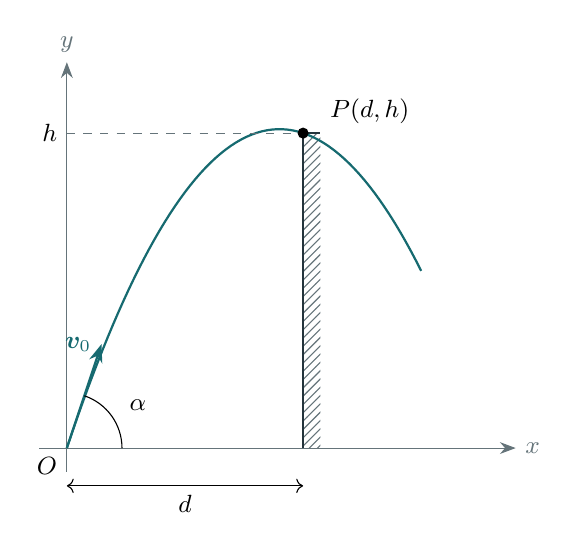
\begin{tikzpicture}[scale=1.0]
\draw[axis] (-.35,0)--(5.7,0) node[right] {$x$};\draw[axis] (0,-.3)--(0,4.9) node[above] {$y$};
\fill[pattern=north east lines,pattern color=muted] (3,0) rectangle (3.22,4);
\draw[object] (3,0)--(3,4)--(3.22,4);
\draw[traj,domain=0:4.5,samples=70] plot(\x,{3*\x-5*\x*\x/9});
\draw[motion] (0,0)--(.44,1.32) node[left] {$\vect v_0$};
\draw (.7,0) arc(0:71.565:.7);\node at (.9,.55) {$\alpha$};
\draw[guide] (0,4)--(3,4);\node[left] at (0,4) {$h$};
\draw[thin,<->] (0,-.48)--(3,-.48) node[midway,below] {$d$};
\fill (3,4) circle (2pt);\node[above right] at (3.22,4) {$P(d,h)$};\node[below left] at (0,0) {$O$};
\end{tikzpicture}
\figcaption{图 1.6\quad 枪口、墙顶与一条通过墙顶的轨迹。}
\end{center}

\workarea

\clearpage

\pdfbookmark[3]{第 7 题 反弹平抛与公共越杆点}{c1-q7}

\section*{第 7 题\quad 反弹平抛与公共越杆点}\label{book-question-1-7}

\tagline{M-01-07}

两个小球从同一点 $S$ 水平抛出，$S$ 距水平地面高 $H$。水平初速分别为 $v_1>v_2>0$。球 1 恰好越过一根竖直杆的顶端，随后第一次落地于 $R$ 点，$OR=R$，其中 $O$ 为 $S$ 在地面的投影。

球 2 第一次落地后，与\textbf{光滑水平地面作完全弹性碰撞}，反弹后恰好越过同一杆顶，并在第二次落地时到达同一 $R$ 点。忽略空气阻力和小球大小。
\begin{enumerate}
\item 求 $v_1/v_2$；\item 求杆的位置 $x_P$；\item 求杆高 $h$。
\end{enumerate}

\begin{center}
\begin{tikzpicture}[x=1cm,y=1.25cm]
\draw[axis] (-.3,0)--(6.6,0) node[right] {$x$};\draw[axis] (0,-.2)--(0,2.75) node[above] {$y$};
\draw[traj,domain=0:6,samples=70] plot(\x,{2.4*(1-\x*\x/36)});
\draw[traj,dashed,domain=0:2,samples=45] plot(\x,{2.4*(1-\x*\x/4)});
\draw[traj,dashed,domain=2:6,samples=70] plot(\x,{2.4*(1-(\x-4)*(\x-4)/4)});
\draw[object,line width=1.3pt] (3,0)--(3,1.8);\fill (3,1.8) circle (1.8pt);
\node[above left] at (0,2.4) {$S$};\node[below left] at (0,0) {$O$};
\node[above left] at (3,1.8) {$P$};\node[below] at (3,0) {$x_P$};
\node[below] at (2,0) {$B$};\node[below] at (6,0) {$R$};
\node[color=accent] at (4.8,1.30) {球 1};\node[color=accent] at (4.4,2.6) {球 2};
\draw[thin,<->] (-.6,0)--(-.6,2.4) node[midway,left] {$H$};
\draw[thin,<->] (3.35,0)--(3.35,1.8) node[midway,right] {$h$};
\end{tikzpicture}
\figcaption{图 1.7\quad 实线为球 1；虚线为球 2；$B$ 为球 2 第一次落地点。}
\end{center}

\workarea

\clearpage

\pdfbookmark[3]{第 8 题 导弹追踪匀速上升飞行物}{c1-q8}

\section*{第 8 题\quad 导弹追踪匀速上升飞行物}\label{book-question-1-8}

\tagline{M-01-08}

飞行物从地面以速率 $v_f>0$ 匀速竖直上升。导弹从距其起飞点水平距离 $L$ 的地面点同时发射。导弹速率 $v$ 恒定，且 $v>v_f$；其瞬时速度方向始终指向飞行物的当前位置。

取导弹发射点为原点，水平朝向目标起飞点为 $x$ 轴，竖直向上为 $y$ 轴，记 $\gamma=v_f/v$。
\begin{enumerate}
\item 求导弹的轨迹 $y(x)$；\item 求击中时间及击中高度。
\end{enumerate}

\begin{center}
\begin{tikzpicture}[x=1cm,y=1cm]
\draw[axis] (-.3,0)--(6.1,0) node[right] {$x$};\draw[axis] (0,-.3)--(0,4.4) node[above] {$y$};
\draw[guide] (5,0)--(5,4.1);\node[below] at (5,0) {$L$};
\draw[traj,domain=0:.998,samples=120] plot({5*\x},{2.5*((1-pow(1-\x,.5))/.5-(1-pow(1-\x,1.5))/1.5)});
\coordinate (M) at (3,.592);\coordinate (F) at (5,1.541);
\draw[guide] (M)--(F);\draw[motion] (M)--(4,1.066) node[midway,above left] {$\vect v$};
\draw[motion] (F)--(5,2.34) node[right] {$v_f$};
\fill (M) circle(2pt);\fill (F) circle(2pt);
\node[below right] at (M) {$M(x,y)$};\node[right] at (F) {$F(L,v_ft)$};
\draw[guide] (3,0)--(M);\node[below] at (3,0) {$x$};
\node[below left] at (0,0) {$O$};\node[right,color=muted] at (5,3.7) {目标航线};
\end{tikzpicture}
\figcaption{图 1.8\quad 导弹轨迹的切线始终沿 $MF$；图中位置对应同一时刻。}
\end{center}

\workarea

\clearpage

\pdfbookmark[3]{第 9 题 圆柱解线与渐开线轨迹}{c1-q9}

\section*{第 9 题\quad 圆柱解线与渐开线轨迹}\label{book-question-1-9}

\tagline{M-01-09}

半径为 $r$ 的圆柱固定不动，轴线竖直。一条很轻、柔软、不可伸长的细线在同一水平面内缠绕于圆柱，线末端系一个可视为质点的小球。初始时小球位于圆柱表面的 $A$ 点，外露直线段长度为零。

给小球一个沿水平方向、垂直于圆柱表面并向外的瞬时冲量，使其初速为 $v$。此后细线无滑动地解开，保持绷紧；忽略重力及其他作用力，并假设缠绕线长足够。
\begin{enumerate}
\item 求 $t>0$ 时小球的加速度大小与方向；
\item 以圆心为原点、$OA$ 为 $x$ 轴正方向，求小球的参数轨迹方程。
\end{enumerate}

\begin{center}
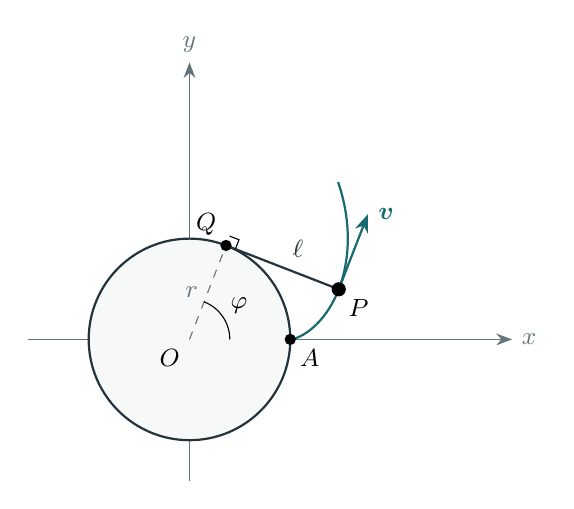
\begin{tikzpicture}[scale=1.28]
\draw[axis] (-1.6,0)--(3.2,0) node[right] {$x$};\draw[axis] (0,-1.4)--(0,2.75) node[above] {$y$};
\draw[object,fill=rulegray!18] (0,0) circle (1);
\draw[traj,domain=0:1.9,samples=90] plot({cos(\x r)+\x*sin(\x r)},{sin(\x r)-\x*cos(\x r)});
\coordinate (Q) at ({cos(1.2 r)},{sin(1.2 r)});
\coordinate (P) at ({cos(1.2 r)+1.2*sin(1.2 r)},{sin(1.2 r)-1.2*cos(1.2 r)});
\draw[object] (Q)--(P) node[midway,above right] {$\ell$};
\draw[guide] (0,0)--(Q) node[midway,left] {$r$};
\draw[motion] (P)--($(P)+(.29,.746)$) node[right] {$\vect v$};
\fill (Q) circle(1.6pt);\fill (P) circle(2pt);\fill (1,0) circle(1.6pt);
\node[above left] at (Q) {$Q$};\node[below right] at (P) {$P$};\node[below right] at (1,0) {$A$};\node[below left] at (0,0) {$O$};
\draw (.4,0) arc(0:68.755:.4);\node at (.49,.34) {$\varphi$};
\draw[thin] ($(Q)+(.093,-.036)$)--($(Q)+(.129,.057)$)--($(Q)+(.036,.093)$);
\end{tikzpicture}
\figcaption{图 1.9\quad $Q$ 为瞬时切点，$QP$ 为解开的直线段；图中选取逆时针展开支。}
\end{center}

\workarea

\clearpage

\pdfbookmark[3]{第 10 题 旋转杆上小环的阿基米德螺线}{c1-q10}

\section*{第 10 题\quad 旋转杆上小环的阿基米德螺线}\label{book-question-1-10}

\tagline{M-01-10}

一根足够长的细杆在固定平面内绕端点 $O$ 以恒定角速度 $\omega>0$ 逆时针旋转。小环可看作质点，沿杆向外的相对速率恒为 $v>0$。设 $t=0$ 时小环位于 $O$，杆沿 $x$ 轴正方向。
\begin{enumerate}
\item 证明小环轨迹为阿基米德螺线；
\item 求任意时刻的速度、加速度向量及其大小；
\item 定性画出加速度在轨迹切向与法向的分量，并说明各自作用。
\end{enumerate}

\begin{center}
\begin{minipage}{\linewidth}\centering
\begin{tikzpicture}[scale=1.1]
\draw[axis] (-2.1,0)--(3.3,0) node[right] {$x$};\draw[axis] (0,-1.9)--(0,3.3) node[above] {$y$};
\draw[traj,domain=0:5.4,samples=120] plot({.45*\x*cos(\x r)},{.45*\x*sin(\x r)});
\coordinate (P) at ({.45*1.1*cos(1.1 r)},{.45*1.1*sin(1.1 r)});
\draw[object,line width=1.2pt] (0,0)--({2.9*cos(1.1 r)},{2.9*sin(1.1 r)});
\filldraw[fill=white,draw=ink,thick] (P) circle(2.4pt);\node[right] at (P) {$P$};
\draw[motion] (.48,.94)--(.94,1.85) node[right] {$v\vect e_r$};
\draw (.34,0) arc(0:63.025:.34);\node at (.65,.2) {$\varphi$};
\draw[motion] (.8,-.45) arc(-29:22:.92);\node[right] at (.98,-.3) {$\omega$};
\node[below left] at (0,0) {$O$};\node[color=muted] at (2.35,2.5) {转动杆};
\end{tikzpicture}
\figcaption{图 1.10\quad 小环沿杆向外运动，同时随杆转动；箭头 $v\vect e_r$ 表示相对速度。}
\end{minipage}
\end{center}

\workarea

\clearpage

\pdfbookmark[3]{第 11 题 相对运动中的最短距离}{c1-q11}

\section*{第 11 题\quad 相对运动中的最短距离}\label{book-question-1-11}

\tagline{M-01-11}

质点甲、乙同时从 $A,B$ 出发，初始距离 $AB=\ell$。甲以速率 $v_1>0$ 沿 $AB$ 向右运动；乙以速率 $v_2>0$ 沿射线 $BC$ 运动。定义 $\alpha=\angle ABC$，即 $BA$ 与 $BC$ 的夹角，$0<\alpha<\pi$。两质点均作匀速直线运动，求出发以后（$t\geq0$）的最短距离。

\begin{center}\begin{minipage}{\linewidth}\centering\begin{tikzpicture}

\coordinate (A) at (0,0);\coordinate (B) at (5,0);\coordinate (C) at (2,2.25);
\draw[object] (A)--(B);\draw[guide] (B)--(C);
\fill (A) circle(2pt);\fill (B) circle(2pt);
\node[below] at (A) {$A$（甲）};\node[below right] at (B) {$B$（乙）};\node[above left] at (C) {$C$};
\draw[motion] (A)--(1.6,0) node[midway,above] {$v_1$};
\draw[motion] (B)--(3.4,1.2) node[midway,above right] {$v_2$};
\draw (4.2,0) arc(180:143.13:.8);\node at (4.05,.32) {$\alpha$};
\draw[thin,<->] (0,-.7)--(5,-.7) node[midway,below] {$\ell$};

\end{tikzpicture}
\figcaption{图 1.11\quad 角 $\alpha$ 从向左的射线 $BA$ 量起。图示为锐角情形。}
\end{minipage}\end{center}

\workarea

\clearpage

\pdfbookmark[3]{第 12 题 非均匀河流中的往返轨迹}{c1-q12}

\section*{第 12 题\quad 非均匀河流中的往返轨迹}\label{book-question-1-12}

\tagline{M-01-12}

宽为 $L$ 的河流沿 $x$ 轴正方向流动。以出发岸为 $y=0$、对岸为 $y=L$，流速大小与到较近河岸的距离成正比：两岸流速为零，河中心流速为 $v_0$。小船从原点出发，相对水以速率 $v_r$ 垂直水流驶向对岸；到 $y=L/4$ 时立即掉头，相对水以速率 $v_r/2$ 垂直水流返回出发岸。忽略掉头所需时间，求两段轨迹及返回点离出发点的距离。

\begin{center}\begin{minipage}{\linewidth}\centering\begin{tikzpicture}

\draw[object] (0,0)--(6,0);\draw[object] (0,3)--(6,3);
\draw[axis] (0,-.2)--(0,3.5) node[above] {$y$};\draw[axis] (0,0)--(6.5,0) node[right] {$x$};
\foreach \y/\a in {.3/.4,.75/1,1.5/2,2.25/1,2.7/.4}{\draw[motion] (3.4,\y)--({3.4+\a},\y);}
\node[right] at (5.4,1.5) {$v_0$};
\draw[guide] (0,.75)--(2.8,.75);\node[left] at (0,.75) {$L/4$};\node[left] at (0,3) {$L$};
\draw[motion] (.4,.12)--(.4,.65) node[left] {$v_r$};
\node[below left] at (0,0) {$O$};

\end{tikzpicture}
\figcaption{图 1.12\quad 流速沿河宽呈三角形分布；小船只在靠近出发岸的四分之一河宽内往返。}
\end{minipage}\end{center}

\workarea

\clearpage

\pdfbookmark[3]{第 13 题 小船始终指向目标的河流轨迹}{c1-q13}

\section*{第 13 题\quad 小船始终指向目标的河流轨迹}\label{book-question-1-13}

\tagline{M-01-13}

笔直河流宽 $d$，水沿 $x$ 轴正方向以恒定速率 $v_0>0$ 流动。取对岸目标 $O$ 为极点，过 $O$ 顺水方向为极轴；出发岸位于 $y=d$。小船从 $A$ 出发，相对水的速率恒为 $v'>v_0$，且相对水的速度方向始终指向 $O$。已知 $OA=r_0$、$\angle AOP=\varphi_0$，其中 $OP$ 顺水，$0<\varphi_0<\pi$，$r_0\sin\varphi_0=d$。求轨迹；另求 $A$ 恰在 $O$ 正对岸时的结果。

\begin{center}\begin{minipage}{\linewidth}\centering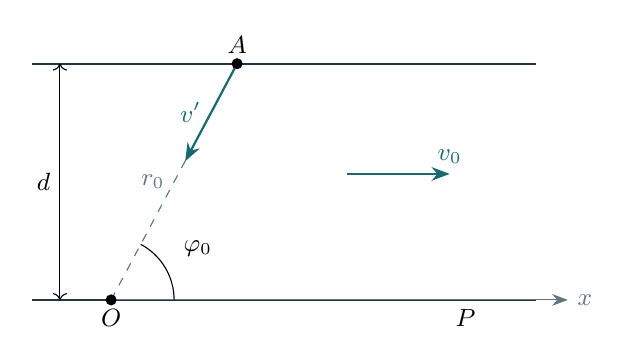
\begin{tikzpicture}

\draw[object] (-1,0)--(5.4,0);\draw[object] (-1,3)--(5.4,3);
\coordinate (O) at (0,0);\coordinate (A) at (1.6,3);
\draw[axis] (O)--(5.8,0) node[right] {$x$};\draw[guide] (O)--(A) node[midway,left] {$r_0$};
\draw[motion] (A)--(.94,1.76) node[midway,left] {$v'$};\draw[motion] (3,1.6)--(4.3,1.6) node[above] {$v_0$};
\draw (.8,0) arc(0:61.93:.8);\node at (1.1,.65) {$\varphi_0$};
\fill (O) circle(2pt);\fill (A) circle(2pt);\node[below] at (O) {$O$};\node[above] at (A) {$A$};\node[below] at (4.5,0) {$P$};
\draw[thin,<->] (-.65,0)--(-.65,3) node[midway,left] {$d$};

\end{tikzpicture}
\figcaption{图 1.13\quad 指向 $O$ 的是相对水速度；对地速度还要加上水流速度。}
\end{minipage}\end{center}

\workarea

\clearpage

\pdfbookmark[3]{第 14 题 纯滚动轮缘点速度}{c1-q14}

\section*{第 14 题\quad 纯滚动轮缘点速度}\label{book-question-1-14}

\tagline{M-01-14}

半径为 $r$ 的轮子在水平面上向右纯滚动。轮心速度为 $v_c$，轮的角速度大小为 $\omega$，转向为顺时针。设接触点为 $M$，轮缘点 $A$ 的位置角 $\theta$ 从 $CM$ 向逆时针量起，$0\leq\theta<2\pi$。求 $A$ 点对地的速度矢量、速率和方向。

\begin{center}\begin{minipage}{\linewidth}\centering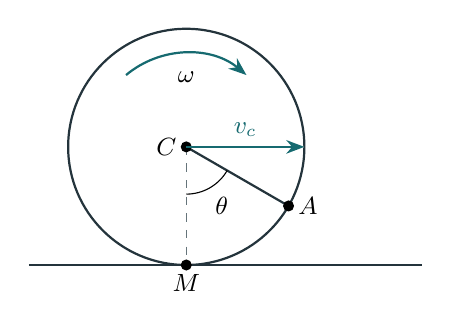
\begin{tikzpicture}

\coordinate (C) at (0,1.5);\coordinate (M) at (0,0);\coordinate (A) at (1.299,.75);
\draw[object] (-2,0)--(3,0);\draw[object] (C) circle(1.5);\draw[guide] (C)--(M);\draw[object] (C)--(A);
\fill (C) circle(2pt);\fill (A) circle(2pt);\fill (M) circle(2pt);
\node[left] at (C) {$C$};\node[below] at (M) {$M$};\node[right] at (A) {$A$};
\draw (0,.9) arc(-90:-30:.6);\node at (.45,.75) {$\theta$};
\draw[motion] (C)--(1.5,1.5) node[midway,above] {$v_c$};
\draw[motion] (-.765,2.412) arc(130:50:1.19);\node at (0,2.38) {$\omega$};

\end{tikzpicture}
\figcaption{图 1.14\quad 轮心平动与绕轮心顺时针转动同时存在。图中 $\theta=60^\circ$。}
\end{minipage}\end{center}

\workarea

\clearpage

\pdfbookmark[3]{第 15 题 内滚圆盘接触点加速度}{c1-q15}

\section*{第 15 题\quad 内滚圆盘接触点加速度}\label{book-question-1-15}

\tagline{M-01-15}

半径 $R$ 的圆环固定，半径 $r<R$ 的圆盘沿圆环内侧无滑动滚动。圆盘中心 $C$ 绕环心 $O$ 以恒定角速度大小 $\Omega$ 运动。求圆盘上在当前时刻与圆环接触的材料点 $A$ 相对圆环的加速度大小和方向。

\begin{center}\begin{minipage}{\linewidth}\centering\begin{tikzpicture}

\coordinate (O) at (0,0);\coordinate (C) at (2,0);\coordinate (A) at (3,0);
\draw[object] (O) circle(3);\draw[guide] (O) circle(2);\draw[object] (C) circle(1);
\draw[object] (O)--(A);\node[below] at (1,0) {$R-r$};\node[below] at (2.5,0) {$r$};
\fill (O) circle(2pt);\fill (C) circle(2pt);\fill (A) circle(2pt);
\node[below left] at (O) {$O$};\node[above] at (C) {$C$};\node[right] at (A) {$A$};
\draw[motion] (1.1,0) arc(0:85:1.1) node[left] {$\Omega$};
\draw[motion] (2.24,.66) arc(70:-40:.7);\node at (2.6,-.8) {$\omega$};
\node[align=left] at (5.9,2) {圆环固定\\圆盘内滚\\当前接触材料点速度为零};

\end{tikzpicture}
\figcaption{图 1.15\quad 盘心逆时针绕 $O$ 运动时，圆盘绕自身中心顺时针转动。}
\end{minipage}\end{center}

\workarea

\clearpage\endgroup


\clearpage
\begingroup
\definecolor{ink}{HTML}{24343C}
\definecolor{accent}{HTML}{166A70}
\definecolor{muted}{HTML}{65747A}
\definecolor{rulegray}{HTML}{D4DDE0}
\definecolor{warm}{HTML}{966037}
\color{ink}
\setlength{\parindent}{2em}
\setlength{\parskip}{4pt}
\linespread{1.12}
\setlength{\abovedisplayskip}{6pt plus 2pt minus 1pt}
\setlength{\belowdisplayskip}{6pt plus 2pt minus 1pt}
\setlength{\abovedisplayshortskip}{0pt plus 1pt}
\setlength{\belowdisplayshortskip}{4pt plus 1pt}
\setlist[enumerate]{label=(\arabic*),leftmargin=2.3em,itemsep=3pt,topsep=4pt}
\setlist[itemize]{leftmargin=2em,itemsep=2pt,topsep=4pt}
\allowdisplaybreaks[1]
\setlength{\emergencystretch}{2em}
\setcounter{secnumdepth}{0}
\providecommand{\tightlist}{\setlength{\itemsep}{0pt}\setlength{\parskip}{0pt}}
\ctexset{section={format=\Large\bfseries\color{accent},beforeskip=10pt,afterskip=9pt},
subsection={format=\normalsize\bfseries\color{accent},beforeskip=10pt,afterskip=4pt},
subsubsection={format=\normalsize\bfseries,beforeskip=8pt,afterskip=3pt}}
\pagestyle{fancy}
\fancyhf{}
\fancyhead[L]{\small\color{muted}物理学难题集萃}
% 页眉仅保留书名；版本名称只在封面显示。
\fancyfoot[L]{\small\color{muted}\chapterlabel}
\fancyfoot[R]{\small\thepage}
\renewcommand{\headrulewidth}{0.4pt}
\renewcommand{\footrulewidth}{0pt}
\renewcommand{\dd}{\mathop{}\!\mathrm{d}}
\renewcommand{\vect}[1]{\bm{#1}}
\renewcommand{\tagline}[1]{\noindent{\small\color{muted}#1}\par}
\renewcommand{\result}[1]{\begin{equation*}\boxed{#1}\end{equation*}}
\renewcommand{\figcaption}[1]{\par\vspace{2pt}{\small\color{muted}#1}\par}
\renewcommand{\teach}[2]{\Needspace{4\baselineskip}\subsection*{讲解要点与追问}#1\par\smallskip\noindent\textbf{追问：}#2\par}
\renewcommand{\workarea}{\par\vspace{7mm}\noindent{\small\color{muted}作答区}\par\vspace{4mm}
\noindent\textcolor{rulegray}{\rule{\linewidth}{0.3pt}}\par\vspace{16mm}
\noindent\textcolor{rulegray}{\rule{\linewidth}{0.3pt}}\par\vspace{16mm}
\noindent\textcolor{rulegray}{\rule{\linewidth}{0.3pt}}\par\vspace{16mm}
\noindent\textcolor{rulegray}{\rule{\linewidth}{0.3pt}}}
\tikzset{axis/.style={-{Stealth[length=2mm]},thin,color=muted},
motion/.style={-{Stealth[length=2.3mm]},thick,color=accent},
force/.style={-{Stealth[length=2.3mm]},thick,color=warm},
traj/.style={thick,color=accent},guide/.style={dashed,thin,color=muted},
object/.style={thick,color=ink},every node/.style={font=\small}}

\renewcommand{\edition}{学生版}
\renewcommand{\chapterlabel}{第二章\quad 牛顿运动定律}


\phantomsection\label{book-unit-2}

\pdfbookmark[1]{第二章 牛顿运动定律}{c2-cover}
\thispagestyle{empty}
\vspace*{20mm}
\noindent{\Huge\bfseries 物理学难题集萃}\par\vspace{8mm}
\noindent{\LARGE 第二章\quad 牛顿运动定律}\par\vspace{10mm}
\noindent{\Large\color{accent}学生版}\par\vspace{8mm}
\noindent\textcolor{accent}{\rule{\linewidth}{1pt}}\par\vspace{8mm}
\noindent 第 1--20 题\par\vspace{5mm}
\noindent 题目、题图与作答区。\par
\vfill\clearpage
\pdfbookmark[2]{题目目录}{c2-contents}
\section*{题目目录}
\begin{longtable}{@{}r p{113mm} r@{}}
\toprule 题号 & 题目 & 页码\\\midrule\endfirsthead
\toprule 题号 & 题目 & 页码\\\midrule\endhead
\bottomrule\endfoot
\hyperref[book-question-2-1]{1} & \hyperref[book-question-2-1]{圆柱绕绳与欧拉摩擦公式} & \pageref{book-question-2-1}\\
\hyperref[book-question-2-2]{2} & \hyperref[book-question-2-2]{旋转斜杆上小环的稳定位置} & \pageref{book-question-2-2}\\
\hyperref[book-question-2-3]{3} & \hyperref[book-question-2-3]{球壳内壁水平圆周运动的速度范围} & \pageref{book-question-2-3}\\
\hyperref[book-question-2-4]{4} & \hyperref[book-question-2-4]{光滑斜面体与滑块的约束加速度} & \pageref{book-question-2-4}\\
\hyperref[book-question-2-5]{5} & \hyperref[book-question-2-5]{旋转球壳中木块的摩擦条件与稳定性} & \pageref{book-question-2-5}\\
\hyperref[book-question-2-6]{6} & \hyperref[book-question-2-6]{反向滚轴上的钢件匀速推动} & \pageref{book-question-2-6}\\
\hyperref[book-question-2-7]{7} & \hyperref[book-question-2-7]{粗糙地面上斜面接触木块的共同加速} & \pageref{book-question-2-7}\\
\hyperref[book-question-2-8]{8} & \hyperref[book-question-2-8]{滑块、绳和悬挂重物的相对静止条件} & \pageref{book-question-2-8}\\
\hyperref[book-question-2-9]{9} & \hyperref[book-question-2-9]{旋转平台沟槽中双球的稳定位置} & \pageref{book-question-2-9}\\
\hyperref[book-question-2-10]{10} & \hyperref[book-question-2-10]{平方阻力竖直上抛的高度与返回速度} & \pageref{book-question-2-10}\\
\hyperref[book-question-2-11]{11} & \hyperref[book-question-2-11]{线性阻力下两竖直质点的相遇} & \pageref{book-question-2-11}\\
\hyperref[book-question-2-12]{12} & \hyperref[book-question-2-12]{线性阻力抛体的轨迹方程} & \pageref{book-question-2-12}\\
\hyperref[book-question-2-13]{13} & \hyperref[book-question-2-13]{飞机着陆滑行距离} & \pageref{book-question-2-13}\\
\hyperref[book-question-2-14]{14} & \hyperref[book-question-2-14]{两根弹簧同时拉断的条件} & \pageref{book-question-2-14}\\
\hyperref[book-question-2-15]{15} & \hyperref[book-question-2-15]{加速斜面上木块相对静止的推力范围} & \pageref{book-question-2-15}\\
\hyperref[book-question-2-16]{16} & \hyperref[book-question-2-16]{双斜面体上两木块相对加速度} & \pageref{book-question-2-16}\\
\hyperref[book-question-2-17]{17} & \hyperref[book-question-2-17]{航天飞机伸杆卫星的潮汐稳定位置} & \pageref{book-question-2-17}\\
\hyperref[book-question-2-18]{18} & \hyperref[book-question-2-18]{旋转圆盘上射手的科里奥利瞄准} & \pageref{book-question-2-18}\\
\hyperref[book-question-2-19]{19} & \hyperref[book-question-2-19]{自由落体的科里奥利偏离} & \pageref{book-question-2-19}\\
\hyperref[book-question-2-20]{20} & \hyperref[book-question-2-20]{傅科摆摆动平面的旋转周期} & \pageref{book-question-2-20}\\
\end{longtable}


\clearpage

\pdfbookmark[3]{第 1 题 圆柱绕绳与欧拉摩擦公式}{c2-q1}

\section*{第 1 题\quad 圆柱绕绳与欧拉摩擦公式}\label{book-question-2-1}

\tagline{M-02-01}

一根质量可忽略的绳绕在固定圆柱上，两端悬挂质量分别为 $M=1000\,\mathrm{kg}$、$m=10\,\mathrm{kg}$ 的桶。绳与圆柱的静摩擦系数为 $\mu=0.050$。按绕线模型，总接触角取 $2\pi n$，$n$ 为完整圈数。要使两桶保持静止，至少需要多少圈？

\begin{center}\begin{minipage}{\linewidth}\centering\begin{tikzpicture}

\draw[object,fill=rulegray!30] (0,.5) rectangle (5,1.9);
\draw[object] (0,1.2) ellipse(.25 and .7);\draw[object] (5,1.2) ellipse(.25 and .7);
\draw[traj,domain=0:5,samples=150] plot(\x,{1.2+.66*sin(216*\x)});
\draw[object] (0,1.2)--(0,-.8);\draw[object] (5,1.2)--(5,-.8);
\draw[object,fill=accent!10] (-.45,-.8) rectangle (.45,-1.45);\node at (0,-1.12) {$m$};
\draw[object,fill=accent!10] (4.3,-.8) rectangle (5.7,-1.8);\node at (5,-1.3) {$M$};
\node[above] at (2.5,2.2) {固定圆柱，绳绕 $n$ 圈};

\end{tikzpicture}
\figcaption{图 2.1\quad 绳绕圆筒连接两端悬桶；所求圈数由绳、筒间的摩擦条件确定。}
\end{minipage}\end{center}

\workarea

\clearpage

\pdfbookmark[3]{第 2 题 旋转斜杆上小环的稳定位置}{c2-q2}

\section*{第 2 题\quad 旋转斜杆上小环的稳定位置}\label{book-question-2-2}

\tagline{M-02-02}

细杆的一端支于地面，以恒定角速度 $\omega>0$ 绕过支点的竖直轴旋转。杆与水平地面的夹角为 $\alpha$，$0<\alpha<\pi/2$。质量 $m$ 的小环套在杆上，静摩擦系数为 $\mu\geq0$。求小环能相对杆保持静止、随杆转动的位置范围，位置以距支点的长度 $L\geq0$ 表示。杆长若有限，取所得范围与实际杆长的交集。

\begin{center}\begin{minipage}{\linewidth}\centering\begin{tikzpicture}

\draw[object] (-.5,0)--(5,0);\draw[axis] (0,-.2)--(0,3.6) node[above] {转轴};
\draw[object,line width=1.2pt] (0,0)--(4,3);\draw[object,fill=accent!15] (2.4,1.8) circle(.15);
\draw[guide] (0,1.8)--(2.4,1.8) node[midway,above] {$L\cos\alpha$};
\draw[thin,<->] (.27,-.36)--(2.67,1.44) node[midway,below right] {$L$};
\draw (.8,0) arc(0:36.87:.8);\node at (1.03,.32) {$\alpha$};
\node[above right] at (2.4,1.8) {$m$};\node[below] at (0,0) {$O$};
\draw[motion] (-.45,3.1) arc(150:-120:.5 and .18) node[left] {$\omega$};

\end{tikzpicture}
\figcaption{图 2.2\quad 小环相对杆静止时，对地作半径 $L\cos\alpha$ 的水平圆周运动。}
\end{minipage}\end{center}

\workarea

\clearpage

\pdfbookmark[3]{第 3 题 球壳内壁水平圆周运动的速度范围}{c2-q3}

\section*{第 3 题\quad 球壳内壁水平圆周运动的速度范围}\label{book-question-2-3}

\tagline{M-02-03}

半径 $R$ 的空心球壳绕竖直直径匀速转动，内壁上一可视为质点的小球相对球壳静止，随球壳沿水平纬度圈以速率 $v$ 运动。小球位于下半球，球心至小球的连线与竖直向下方向的夹角为 $\theta$，$0<\theta<\pi/2$。静摩擦系数为 $\mu\geq0$。求在该纬度能维持共转的速率范围。
\par\smallskip\begin{center}\begin{minipage}{\linewidth}\centering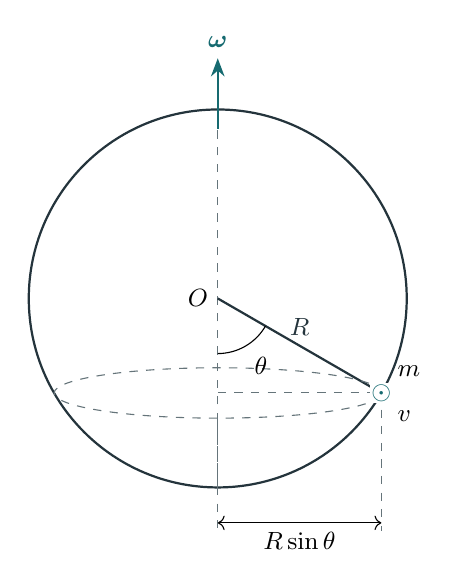
\begin{tikzpicture}
\draw[object] (0,0) circle(2.4);
\draw[guide] (0,-2.4)--(0,2.35);
\coordinate (B) at (2.078,-1.2);
\draw[object] (0,0)--(B) node[midway,above] {$R$};
\draw[guide] (0,-1.2) ellipse(2.078 and .32);
\draw[guide] (0,-1.2)--(B);
\draw[guide] (0,-1.55)--(0,-2.95);
\draw[guide] (B)--(2.078,-2.95);
\draw[<->] (0,-2.85)--(2.078,-2.85) node[midway,below] {$R\sin\theta$};
\node[fill=white,inner sep=.4pt,text=accent] at (B) {$\odot$};
\node[above right] at (2.16,-1.12) {$m$};
\node[below right] at (2.16,-1.3) {$v$};
\node[left] at (0,0) {$O$};
\draw (0,-.7) arc(-90:-30:.7);
\node at (.55,-.85) {$\theta$};
\draw[motion] (0,2.15)--(0,3.05) node[above] {$\boldsymbol\omega$};
\end{tikzpicture}
\figcaption{图 2.3\quad 纬度圈半径为$R\sin\theta$；$\odot$表示周向速度垂直子午面朝向观察者。}
\end{minipage}\end{center}

\workarea

\clearpage

\pdfbookmark[3]{第 4 题 光滑斜面体与滑块的约束加速度}{c2-q4}

\section*{第 4 题\quad 光滑斜面体与滑块的约束加速度}\label{book-question-2-4}

\tagline{M-02-04}

倾角为 $\theta$、质量为 $M$ 的斜面体放在光滑水平地面上，质量为 $m$ 的木块放在斜面上，接触面也光滑。斜面从左下向右上倾斜，$0<\theta<\pi/2$。求斜面体与木块相对地面的加速度，以及木块所受支持力。

\begin{center}\begin{minipage}{\linewidth}\centering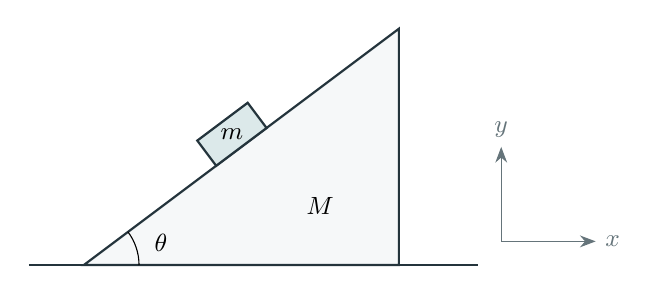
\begin{tikzpicture}

\draw[object] (-.7,0)--(5,0);\draw[object,fill=rulegray!20] (0,0)--(4,3)--(4,0)--cycle;
\begin{scope}[shift={(1.88,1.66)},rotate=36.87]\draw[object,fill=accent!15] (-.4,-.2) rectangle (.4,.2);\node at (0,0) {$m$};\end{scope}
\node at (3,.75) {$M$};\draw (.7,0) arc(0:36.87:.7);\node at (.98,.28) {$\theta$};
\draw[axis] (5.3,.3)--(6.5,.3) node[right] {$x$};\draw[axis] (5.3,.3)--(5.3,1.5) node[above] {$y$};

\end{tikzpicture}
\figcaption{图 2.4\quad 木块下滑时，斜面体向右运动；两者加速度均按地面坐标描述。}
\end{minipage}\end{center}

\workarea

\clearpage

\pdfbookmark[3]{第 5 题 旋转球壳中木块的摩擦条件与稳定性}{c2-q5}

\section*{第 5 题\quad 旋转球壳中木块的摩擦条件与稳定性}\label{book-question-2-5}

\tagline{M-02-05}

半径 $R=0.5\,\mathrm m$ 的空心球壳绕竖直直径匀速转动。内壁上的小木块可看作质点，位于距球壳最低点 $h=R/2$ 的高度，随壳共转。取 $g=9.8\,\mathrm{m/s^2}$。
\begin{enumerate}
\item 当 $\omega=5\,\mathrm{s^{-1}}$ 时，至少需要多大的静摩擦系数？
\item 当 $\omega=8\,\mathrm{s^{-1}}$ 时，维持共转的条件是什么？
\item 分别讨论木块位置、角速度发生微小改变后能否继续共转。区分静摩擦有余量和恰好临界的情形，说明仅由这些条件能否断言木块必定返回原位置。
\end{enumerate}

\begin{center}\begin{minipage}{\linewidth}\centering\begin{tikzpicture}

\draw[object] (0,0) circle(2.4);\draw[guide] (0,-2.4)--(0,2.4);
\coordinate (B) at (2.078,-1.2);\draw[object] (0,0)--(B);\draw[guide] (0,-1.2)--(B);
\fill (B) circle(2.5pt);\node[right] at (B) {木块};\node[left] at (0,0) {$O$};
\draw (0,-.7) arc(-90:-30:.7);\node at (.55,-.85) {$\theta$};
\draw[thin,<->] (2.75,-2.4)--(2.75,-1.2) node[midway,right] {$h=R/2$};
\draw[guide] (0,-2.4)--(2.75,-2.4);\draw[guide] (B)--(2.75,-1.2);
\draw[motion] (-.45,2.05) arc(150:-120:.5 and .18) node[left] {$\omega$};

\end{tikzpicture}
\figcaption{图 2.5\quad 高度从球壳最低点量起，$h=R(1-\cos\theta)$，本题 $\theta=60^\circ$。}
\end{minipage}\end{center}

\workarea

\clearpage

\pdfbookmark[3]{第 6 题 反向滚轴上的钢件匀速推动}{c2-q6}

\section*{第 6 题\quad 反向滚轴上的钢件匀速推动}\label{book-question-2-6}

\tagline{M-02-06}

质量 $m=20\,\mathrm{kg}$ 的对称钢件架在两个相同的平行长直滚轴上。滚轴轴线水平，半径 $r=0.025\,\mathrm m$，以角速度 $\omega=40\,\mathrm{rad/s}$ 反向转动，接触处的表面速度大小均为 $\omega r$，方向水平且相反。钢件与滚轴间的滑动摩擦系数 $\mu=0.20$。要使钢件沿滚轴轴线以 $v_0=0.050\,\mathrm{m/s}$ 匀速运动，需施加多大的轴向水平力 $F$？取 $g=10\,\mathrm{m/s^2}$。

\begin{center}\begin{minipage}{\linewidth}\centering\begin{tikzpicture}

\draw[object] (0,0) ellipse(.45 and .22);\draw[object] (0,0)--(0,3);\draw[object] (.45,0)--(.45,3);\draw[object] (-.45,0)--(-.45,3);\draw[object] (0,3) ellipse(.45 and .22);
\draw[object] (3,0) ellipse(.45 and .22);\draw[object] (3,0)--(3,3);\draw[object] (3.45,0)--(3.45,3);\draw[object] (2.55,0)--(2.55,3);\draw[object] (3,3) ellipse(.45 and .22);
\filldraw[object,fill=white] (-.7,.9) rectangle (3.7,2);\node at (1.5,1.45) {钢件};
\draw[motion] (0,2.6)--(-1.2,2.6) node[left] {$\omega r$};\draw[motion] (3,2.6)--(4.2,2.6) node[right] {$\omega r$};
\draw[motion] (1.5,2)--(1.5,3.6) node[above] {$v_0,F$};\node at (1.5,-.6) {俯视图：图中上下方向沿滚轴轴线};

\end{tikzpicture}
\figcaption{图 2.6\quad 两接触处的横向表面速度相反。}
\end{minipage}\end{center}

\workarea

\clearpage

\pdfbookmark[3]{第 7 题 粗糙地面上斜面接触木块的共同加速}{c2-q7}

\section*{第 7 题\quad 粗糙地面上斜面接触木块的共同加速}\label{book-question-2-7}

\tagline{M-02-07}

质量为 $m_A,m_B$ 的木块 $A,B$ 放在粗糙水平地面上，与地面的摩擦系数均为 $\mu$。两木块接触面光滑，倾角 $0<\theta<\pi/2$，其方向如图：$A$ 对 $B$ 的压力向右下方。水平推力 $F$ 作用于 $A$，使两木块向右加速且无相对滑动。以下讨论两块已经向右滑动、地面采用滑动摩擦的平动阶段。求 $\mu$ 和 $F$ 的条件。允许 $A$ 的地面支持力恰好为零。

\begin{center}\begin{minipage}{\linewidth}\centering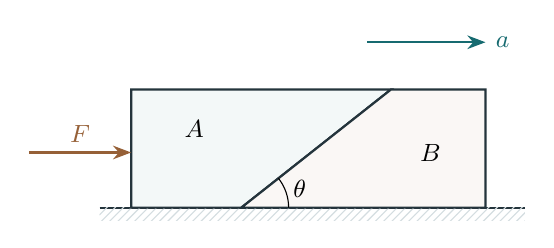
\begin{tikzpicture}

\draw[object] (-.4,0)--(5,0);\fill[pattern=north east lines,pattern color=rulegray] (-.4,-.16) rectangle (5,0);
\filldraw[object,fill=accent!5] (0,0)--(1.4,0)--(3.3,1.5)--(0,1.5)--cycle;
\filldraw[object,fill=warm!5] (1.4,0)--(4.5,0)--(4.5,1.5)--(3.3,1.5)--cycle;
\node at (.8,1) {$A$};\node at (3.8,.7) {$B$};
\draw[force] (-1.3,.7)--(0,.7) node[midway,above] {$F$};
\draw (2,0) arc(0:38.29:.6);\node at (2.14,.24) {$\theta$};\draw[motion] (3,2.1)--(4.5,2.1) node[right] {$a$};

\end{tikzpicture}
\figcaption{图 2.7\quad 接触斜面向右升高；两木块都与地面保持接触。}
\end{minipage}\end{center}

\workarea

\clearpage

\pdfbookmark[3]{第 8 题 滑块、绳和悬挂重物的相对静止条件}{c2-q8}

\section*{第 8 题\quad 滑块、绳和悬挂重物的相对静止条件}\label{book-question-2-8}

\tagline{M-02-08}

质量为 $M$ 的滑块 $C$ 位于光滑水平桌面上，滑轮固定在滑块右端。质量均为 $m$ 的物体 $A,B$ 用轻绳连接：$A$ 放在滑块上，绳的这一段水平；$B$ 悬在滑轮外侧。$A$ 与滑块的静摩擦系数为 $\mu$，绳和滑轮质量忽略，转轴光滑。用水平力 $F\geq0$ 向右推动滑块。求使 $A,B$ 与滑块保持相对静止的最小推力。讨论已建立的共同加速状态，悬绳允许倾斜，且 $B$ 不接触滑块。

\begin{center}\begin{minipage}{\linewidth}\centering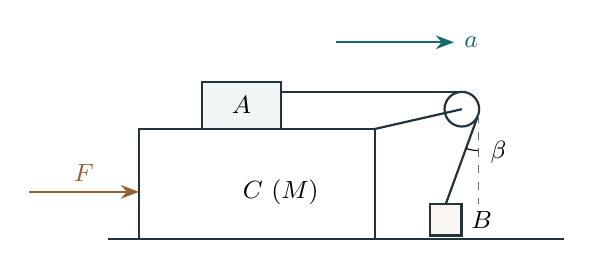
\begin{tikzpicture}

\draw[object] (-.4,0)--(5.4,0);\draw[object] (0,0) rectangle (3,1.4);\node at (1.8,.6) {$C\ (M)$};
\filldraw[object,fill=accent!6] (.8,1.4) rectangle (1.8,2);\node at (1.3,1.7) {$A$};
\draw[object] (4.1,1.65) circle(.22);\draw[object] (3,1.4)--(4.1,1.65);\draw[object] (1.8,1.87)--(4.1,1.87);
\draw[object] (4.3067,1.5748)--(3.8963,.4471);\filldraw[object,fill=warm!6] (3.6963,.0471) rectangle (4.0963,.4471);\node[right] at (4.0963,.2471) {$B$};
\draw[guide] (4.3067,1.5748)--(4.3067,.45);\draw (4.3067,1.1248) arc(270:250:.45);\node[right] at (4.34,1.10) {$\beta$};
\draw[force] (-1.4,.6)--(0,.6) node[midway,above] {$F$};\draw[motion] (2.5,2.5)--(4,2.5) node[right] {$a$};

\end{tikzpicture}
\figcaption{图 2.8\quad 共同向右加速时，悬绳向左倾斜。图中的侧面留有间隙，表示 $B$ 不与滑块接触。}
\end{minipage}\end{center}

\workarea

\clearpage

\pdfbookmark[3]{第 9 题 旋转平台沟槽中双球的稳定位置}{c2-q9}

\section*{第 9 题\quad 旋转平台沟槽中双球的稳定位置}\label{book-question-2-9}

\tagline{M-02-09}

水平平台以角速度 $\omega>0$ 绕中心竖直轴转动。两个径向沟槽内分别放小球 $A,B$，质量为 $m_A,m_B$。$A$ 与槽底的静摩擦系数为 $\mu$，$B$ 所在槽光滑。长为 $\ell$ 的轻绳绕过光滑中心轴，连接两球；轴半径可忽略。求两球可以与平台保持相对静止时，$A$ 到中心的距离 $x$ 的范围。忽略球和轴的尺寸，槽长至少为 $\ell$。

\begin{center}\begin{minipage}{\linewidth}\centering\begin{tikzpicture}

\draw[object] (0,0) circle(2.4);\draw[object] (-2.2,.17)--(2.2,.17);\draw[object] (-2.2,-.17)--(2.2,-.17);
\draw[object] (-1.55,0)--(1.2,0);\filldraw[object,fill=accent!12] (-1.55,0) circle(.15);\filldraw[object,fill=warm!12] (1.2,0) circle(.15);\fill (0,0) circle(2pt);
\node[above] at (-1.55,.2) {$A$（粗糙）};\node[above] at (1.2,.2) {$B$（光滑）};\node[below] at (0,0) {$O$};
\draw[thin,<->] (-1.55,-.6)--(0,-.6) node[midway,below] {$x$};\draw[thin,<->] (0,-.6)--(1.2,-.6) node[midway,below] {$\ell-x$};
\draw[motion] (2.75,-.7) arc(-15:55:2.85);\node[right] at (2.7,.8) {$\omega$};

\end{tikzpicture}
\figcaption{图 2.9\quad 绳长把两个向心运动联系起来，槽沿半径方向。}
\end{minipage}\end{center}

\workarea

\clearpage

\pdfbookmark[3]{第 10 题 平方阻力竖直上抛的高度与返回速度}{c2-q10}

\section*{第 10 题\quad 平方阻力竖直上抛的高度与返回速度}\label{book-question-2-10}

\tagline{M-02-10}

质量 $m$ 的物体从地面以速率 $v_0$ 竖直上抛。空气阻力大小为 $\mu v^2$，方向与速度相反，$\mu>0$ 为常数，重力加速度为 $g$。求最大高度，并证明返回地面时的速率为 $v_0\sqrt{mg/(mg+\mu v_0^2)}$。

\begin{center}\begin{minipage}{\linewidth}\centering\begin{tikzpicture}

\draw[object] (-.7,0)--(4.5,0);\draw[axis] (-.3,0)--(-.3,3.5) node[above] {$y$};
\draw[motion] (.7,.2)--(.7,2.9) node[midway,left] {上升};\draw[motion] (2.8,2.9)--(2.8,.2) node[midway,right] {下降};
\draw[guide] (.3,3.1)--(3.3,3.1);\node[right] at (3.3,3.1) {$H$};\node[below] at (.7,0) {$v_0$};\node[below] at (2.8,0) {$u_f$};

\end{tikzpicture}
\figcaption{图 2.10\quad 最高点前后阻力反向，需分别列方程。}
\end{minipage}\end{center}

\workarea

\clearpage

\pdfbookmark[3]{第 11 题 线性阻力下两竖直质点的相遇}{c2-q11}

\section*{第 11 题\quad 线性阻力下两竖直质点的相遇}\label{book-question-2-11}

\tagline{M-02-11}

两个质量均为 $m$ 的质点同时开始运动：质点 1 从离地高度 $h$ 处由静止下落；质点 2 从它正下方的地面以初速 $v_0>0$ 竖直上抛。空气阻力为 $\vect f=-\mu\vect v$，$\mu>0$。求相遇时间、高度和两者相遇时的速度，并判断相遇是否发生在落地以前。不讨论质点接触地面后的运动。

\begin{center}\begin{minipage}{\linewidth}\centering\begin{tikzpicture}

\draw[object] (-.6,0)--(3.5,0);\draw[axis] (-.4,0)--(-.4,3.6) node[above] {$y$};
\filldraw[object,fill=accent!10] (1,3) circle(.12);\filldraw[object,fill=warm!10] (1,.12) circle(.12);
\node[right] at (1.15,3) {1：初速为零};\node[right] at (1.15,.12) {2};\draw[motion] (1,.4)--(1,1.5) node[right] {$v_0$};
\draw[thin,<->] (2.8,0)--(2.8,3) node[midway,right] {$h$};

\end{tikzpicture}
\figcaption{图 2.11\quad 速度统一以向上为正，阻力表达式适用于上升和下降。}
\end{minipage}\end{center}

\workarea

\clearpage

\pdfbookmark[3]{第 12 题 线性阻力抛体的轨迹方程}{c2-q12}

\section*{第 12 题\quad 线性阻力抛体的轨迹方程}\label{book-question-2-12}

\tagline{M-02-12}

质量 $m$ 的抛射体从原点以初速 $v_0$、仰角 $0<\alpha<\pi/2$ 发射。空气阻力为 $\vect f=-k\vect v$，$k>0$，重力加速度为 $g$。求轨迹方程 $y(x)$，说明其适用的 $x$ 范围，并验证 $k\to0$ 时得到通常的抛物线方程。

\begin{center}\begin{minipage}{\linewidth}\centering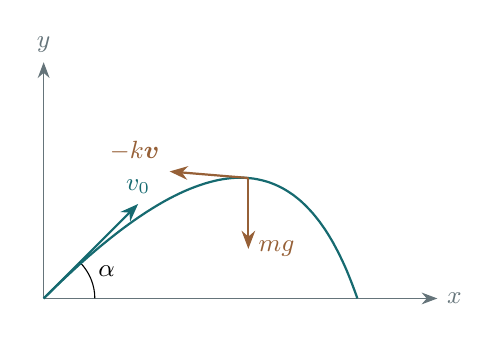
\begin{tikzpicture}

\draw[axis] (0,0)--(5,0) node[right] {$x$};\draw[axis] (0,0)--(0,3) node[above] {$y$};
\draw[motion] (0,0)--(1.2,1.2) node[above] {$v_0$};\draw (.65,0) arc(0:45:.65);\node at (.8,.35) {$\alpha$};
\draw[traj,domain=0:2.656,samples=80] plot({5*(1-exp(-.6*\x))},{10*(1-exp(-.6*\x))-3*\x});
\draw[force] (2.6,1.53)--(1.6,1.613) node[above left] {$-k\vect v$};\draw[force] (2.6,1.53)--(2.6,.63) node[right] {$mg$};

\end{tikzpicture}
\figcaption{图 2.12\quad 阻力与瞬时速度反向，水平分量使 $v_x$ 持续衰减。}
\end{minipage}\end{center}

\workarea

\clearpage

\pdfbookmark[3]{第 13 题 飞机着陆滑行距离}{c2-q13}

\section*{第 13 题\quad 飞机着陆滑行距离}\label{book-question-2-13}

\tagline{M-02-13}

飞机以水平速度 $v_0=90\,\mathrm{km/h}$ 触地滑行。空气阻力为 $c_xv^2$，机翼升力为 $c_yv^2$，$c_y/c_x=k=5$；轮胎与跑道间的有效摩擦系数为 $\mu=0.10$。假设刚触地时升力恰等于重力，随后 $c_x,c_y$ 不变，忽略发动机推力。求停止前的滑行距离，取 $g=9.8\,\mathrm{m/s^2}$。

\begin{center}\begin{minipage}{\linewidth}\centering\begin{tikzpicture}

\draw[object] (-.6,0)--(5.3,0);\draw[object] (.2,.6)--(3.4,.6)--(3.8,.9)--(3.5,1.15)--(.9,1.15)--(.2,.6);\draw[object] (.7,.9)--(.2,1.7)--(.65,1.7)--(1.1,1.15);
\draw[object] (1.1,.25) circle(.25);\draw[object] (2.9,.25) circle(.25);\draw[object] (1.1,.50)--(1.1,.8);\draw[object] (2.9,.50)--(2.9,.8);
\draw[motion] (4,.9)--(5.3,.9) node[right] {$v$};\node at (2.2,-.55) {升力随速度降低，轮胎压力增大};

\end{tikzpicture}
\figcaption{图 2.13\quad 滑行减速时，空气阻力减小，地面摩擦增大。}
\end{minipage}\end{center}

\workarea

\clearpage

\pdfbookmark[3]{第 14 题 两根弹簧同时拉断的条件}{c2-q14}

\section*{第 14 题\quad 两根弹簧同时拉断的条件}\label{book-question-2-14}

\tagline{M-02-14}

质量 $m$ 的小球用轻弹簧 1 竖直悬挂，劲度系数为 $k$。小球下方再接相同的轻弹簧 2，在其下端施加向下的拉力 $F(t)=\alpha t$，$\alpha>0$。两弹簧伸长达到 $\ell_C$ 时断裂，且 $\ell_C>mg/k$。$t=0$ 时小球静止于原平衡位置、下弹簧无伸长。求两弹簧同时首次达到断裂伸长时 $\alpha$ 应满足的关系式。

\begin{center}\begin{minipage}{\linewidth}\centering\begin{tikzpicture}

\draw[object] (-.8,3.6)--(.8,3.6);\draw[object] (0,3.6)--(0,3.4)--(-.15,3.25)--(.15,3.05)--(-.15,2.85)--(.15,2.65)--(-.15,2.45)--(0,2.3)--(0,2.15);
\filldraw[object,fill=accent!10] (0,1.9) circle(.25);\node[right] at (.3,1.9) {$m$};\node[left] at (-.35,2.9) {弹簧 1};
\draw[object] (0,1.65)--(0,1.5)--(-.15,1.35)--(.15,1.15)--(-.15,.95)--(.15,.75)--(-.15,.55)--(0,.4)--(0,.2);
\node[left] at (-.35,1) {弹簧 2};\draw[force] (0,.2)--(0,-.7) node[below] {$F=\alpha t$};
\draw[axis] (2,3.2)--(2,.3) node[below] {向下为正};

\end{tikzpicture}
\figcaption{图 2.14\quad 两根弹簧相同，伸长的时间变化却不同。}
\end{minipage}\end{center}

\workarea

\clearpage

\pdfbookmark[3]{第 15 题 加速斜面上木块相对静止的推力范围}{c2-q15}

\section*{第 15 题\quad 加速斜面上木块相对静止的推力范围}\label{book-question-2-15}

\tagline{M-02-15}

质量 $M$ 的斜面体位于光滑水平桌面上，斜面向右下降，倾角为 $0<\theta<\pi/2$。质量 $m$ 的木块置于斜面上，静摩擦系数 $0\leq\mu<\tan\theta$。水平力 $F\geq0$ 向右推斜面体。求木块可以相对斜面静止的推力范围；忽略斜面边缘对运动的限制。

\begin{center}\begin{minipage}{\linewidth}\centering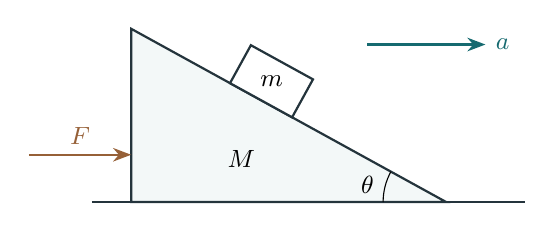
\begin{tikzpicture}

\draw[object] (-.5,0)--(5,0);\filldraw[object,fill=accent!5] (0,0)--(4,0)--(0,2.2)--cycle;\node at (1.4,.55) {$M$};
\begin{scope}[shift={(1.65,1.2925)},rotate=-28.81]\filldraw[object,fill=white] (-.45,0) rectangle (.45,.55);\node at (0,.28) {$m$};\end{scope}
\draw[force] (-1.3,.6)--(0,.6) node[midway,above] {$F$};\draw (3.2,0) arc(180:151.19:.8);\node at (3,.22) {$\theta$};\draw[motion] (3,2)--(4.5,2) node[right] {$a$};

\end{tikzpicture}
\figcaption{图 2.15\quad 方向约定：推力向右，斜面向右下降。}
\end{minipage}\end{center}

\workarea

\clearpage

\pdfbookmark[3]{第 16 题 双斜面体上两木块相对加速度}{c2-q16}

\section*{第 16 题\quad 双斜面体上两木块相对加速度}\label{book-question-2-16}

\tagline{M-02-16}

质量 $M$ 的双斜面体位于光滑水平地面上，左右坡面的倾角分别为 $\alpha_1,\alpha_2\in(0,\pi/2)$。质量为 $m_1,m_2$ 的两木块分别放在左右坡面，用轻绳经过固定在斜面体顶部的轻滑轮连接。接触面和滑轮均光滑，绳不可伸长。在两块都沿各自坡面运动的阶段，求它们相对斜面体的加速度、斜面体相对地面的加速度，以及两块保持接触的条件。

\begin{center}\begin{minipage}{\linewidth}\centering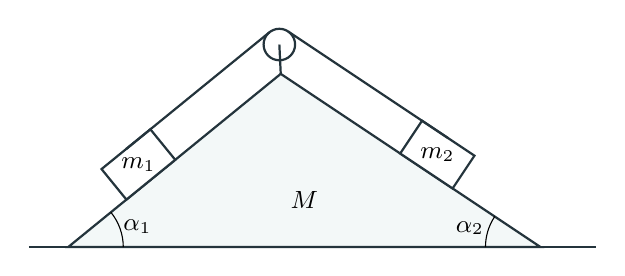
\begin{tikzpicture}

\draw[object] (-.5,0)--(6.7,0);\filldraw[object,fill=accent!5] (0,0)--(6,0)--(2.7,2.2)--cycle;\node at (3,.6) {$M$};
\draw[object] (2.682164,2.572446) circle(.2);\draw[object] (2.7,2.2)--(2.682164,2.572446);
\begin{scope}[shift={(1.05,.8556)},rotate=39.17366]\filldraw[object,fill=white] (-.4,0) rectangle (.4,.5);\node at (0,.25) {$m_1$};\end{scope}
\begin{scope}[shift={(4.55,.9667)},rotate=-33.69007]\filldraw[object,fill=white] (-.4,0) rectangle (.4,.5);\node at (0,.25) {$m_2$};\end{scope}
\draw[object] (.734164,1.243173)--(2.555829,2.727493);\draw[object] (2.793104,2.738856)--(4.827350,1.382692);
\draw (.7,0) arc(0:39.17:.7);\node at (.88,.26) {$\alpha_1$};\draw (5.3,0) arc(180:146.31:.7);\node at (5.1,.24) {$\alpha_2$};

\end{tikzpicture}
\figcaption{图 2.16\quad 两木块相对斜面体沿绳方向运动，一边下滑时另一边上滑。}
\end{minipage}\end{center}

\workarea

\clearpage

\pdfbookmark[3]{第 17 题 航天飞机伸杆卫星的潮汐稳定位置}{c2-q17}

\section*{第 17 题\quad 航天飞机伸杆卫星的潮汐稳定位置}\label{book-question-2-17}

\tagline{M-02-17}

质量 $m_1$ 的航天飞机 $A$ 绕地球作半径 $R$ 的圆轨道运动。它通过一根长 $L$ 的轻刚杆连接质量 $m_2$ 的卫星 $S$，$L\ll R$、$m_2\ll m_1$。将 $A,S$ 看作质点，杆可在轨道平面内自由转动，不施加姿态控制力矩。定义 $\alpha$ 为杆 $AS$ 从指向地心的方向量起的角度，方向见图。求相对轨道转动系的平衡方位并讨论小扰动稳定性。

\begin{center}\begin{minipage}{\linewidth}\centering\begin{tikzpicture}

\coordinate (E) at (0,0);\coordinate (A) at (4,0);\coordinate (S) at (2.75,1.1);
\draw[object] (E) circle(.45);\node[below] at (0,-.45) {地球};\draw[guide] (E)--(A);\draw[object] (A)--(S);
\fill (A) circle(2pt);\fill (S) circle(2pt);\node[right] at (A) {$A$};\node[above left] at (S) {$S$};\node[above right] at (3.4,.6) {$L$};\node[below] at (2,0) {$R$};
\draw (3.4,0) arc(180:138.65:.6);\node at (3.2,.32) {$\alpha$};\draw[motion] (4,-.8)--(4,.85) node[above] {轨道速度};

\end{tikzpicture}
\figcaption{图 2.17\quad $\alpha=0$ 表示卫星位于航天飞机朝地心的一侧。}
\end{minipage}\end{center}

\workarea

\clearpage

\pdfbookmark[3]{第 18 题 旋转圆盘上射手的科里奥利瞄准}{c2-q18}

\section*{第 18 题\quad 旋转圆盘上射手的科里奥利瞄准}\label{book-question-2-18}

\tagline{M-02-18}

半径 $R$ 的水平圆盘以角速度 $\omega>0$ 逆时针转动。发射瞬间，盘边缘射手 $A=(-R,0)$ 的目标位于直径另一端 $B=(R,0)$。子弹相对圆盘的初速大小为 $v_0$，且 $\varepsilon=\omega R/v_0\ll1$。忽略空气阻力，只讨论水平运动，飞行很短而略去竖直下落。射手应朝哪个方向瞄准？求盘上观察到的轨迹，保留 $\varepsilon$ 的一阶项，并说明圆弧近似的适用性。

\begin{center}\begin{minipage}{\linewidth}\centering\begin{tikzpicture}

\draw[object] (0,0) circle(2);\draw[guide] (-2,0)--(2,0);\fill (-2,0) circle(2pt);\fill (2,0) circle(2pt);\fill (0,0) circle(2pt);
\node[left] at (-2,0) {$A$};\node[right] at (2,0) {$B$};\node[below] at (0,0) {$O$};
\draw[motion] (-2,0)--(-.2,.7) node[above] {$v_0$};\draw (-1.4,0) arc(0:21.25:.6);\node at (-1.25,.16) {$\theta$};
\draw[motion] (2,0)--(2,.9) node[right] {$B$ 的速度};\draw[motion] (-2,0)--(-2,-.9) node[left] {$A$ 的速度};\draw[motion] (2.4,-.4) arc(-9.5:45:2.43);\node[above right] at (2,2.05) {$\omega$};

\end{tikzpicture}
\figcaption{图 2.18\quad 逆时针转动时，目标向上走，射手所在处的牵连速度向下。偏角作放大示意。}
\end{minipage}\end{center}

\workarea

\clearpage

\pdfbookmark[3]{第 19 题 自由落体的科里奥利偏离}{c2-q19}

\section*{第 19 题\quad 自由落体的科里奥利偏离}\label{book-question-2-19}

\tagline{M-02-19}

地球以角速度 $\omega$ 自转。纬度为 $\varphi$ 的地点上空，高度 $h$ 处一质点相对地面由静止释放。忽略空气阻力和离心惯性力，取局部重力加速度 $g$ 为常量，落下高度远小于地球半径。求科里奥利力引起的落地点偏离，先求 $\omega$ 一阶的主要偏移，再给出该局部模型中二阶的南北偏移。

\begin{center}\begin{minipage}{\linewidth}\centering\begin{tikzpicture}

\draw[axis] (0,0)--(3,0) node[right] {$x$，东};\draw[axis] (0,0)--(-1.2,-1.1) node[below left] {$y$，北};\draw[axis] (0,0)--(0,3.3) node[above] {$z$，上};
\fill (0,2.7) circle(2pt);\draw[motion] (0,2.4)--(0,1.4) node[left] {下落};\draw[guide] (.45,2.7)--(.45,0);\node[right] at (.45,1.7) {$h$};
\draw[motion] (-2.4,1)--(-3.1,2.2) node[above] {$\vect\omega$};\node[align=left] at (4,2) {$\omega_y=\omega\cos\varphi$\\$\omega_z=\omega\sin\varphi$};

\end{tikzpicture}
\figcaption{图 2.19\quad 局部坐标依次为东、北、上，组成右手系。自转矢量以北半球为例绘出。}
\end{minipage}\end{center}

\workarea

\clearpage

\pdfbookmark[3]{第 20 题 傅科摆摆动平面的旋转周期}{c2-q20}

\section*{第 20 题\quad 傅科摆摆动平面的旋转周期}\label{book-question-2-20}

\tagline{M-02-20}

傅科摆在纬度 $\varphi$ 的地点作小角度摆动，地球自转角速度为 $\omega$，自转周期为 $T_0=2\pi/\omega$。忽略阻尼和离心项，且 $\omega$ 远小于摆的固有频率。证明摆动方向相对地面的进动角速度为 $-\omega\sin\varphi$，并求完整进动一周的周期。说明南北半球和赤道的情形。

\begin{center}\begin{minipage}{\linewidth}\centering\begin{tikzpicture}

\draw[object] (-.7,3.2)--(.7,3.2);\draw[object] (0,3.2)--(.6,.4);\filldraw[object,fill=accent!10] (.6,.4) circle(.15);\draw[guide] (0,3.2)--(0,.2);
\draw[object] (0,0) ellipse(1.6 and .45);\draw[traj] (-1.4,-.15)--(1.4,.15);\draw[guide] (-1.1,.31)--(1.1,-.31);\node at (0,-.8) {摆动方向随时间缓慢改变};
\node[align=left] at (4.6,2) {$\Omega=\omega\sin\varphi$\\自转的竖直分量};

\end{tikzpicture}
\figcaption{图 2.20\quad 摆的快振动与摆动方向的慢进动同时发生。}
\end{minipage}\end{center}

\workarea

\clearpage\endgroup


\clearpage
\begingroup
\definecolor{ink}{HTML}{24343C}
\definecolor{accent}{HTML}{166A70}
\definecolor{muted}{HTML}{65747A}
\definecolor{rulegray}{HTML}{D4DDE0}
\definecolor{warm}{HTML}{966037}
\color{ink}
\setlength{\parindent}{2em}
\setlength{\parskip}{4pt}
\linespread{1.12}
\setlength{\abovedisplayskip}{6pt plus 2pt minus 1pt}
\setlength{\belowdisplayskip}{6pt plus 2pt minus 1pt}
\setlength{\abovedisplayshortskip}{0pt plus 1pt}
\setlength{\belowdisplayshortskip}{4pt plus 1pt}
\setlist[enumerate]{label=(\arabic*),leftmargin=2.3em,itemsep=3pt,topsep=4pt}
\setlist[itemize]{leftmargin=2em,itemsep=2pt,topsep=4pt}
\allowdisplaybreaks[1]
\setlength{\emergencystretch}{2em}
\setcounter{secnumdepth}{0}
\providecommand{\tightlist}{\setlength{\itemsep}{0pt}\setlength{\parskip}{0pt}}
\ctexset{section={format=\Large\bfseries\color{accent},beforeskip=10pt,afterskip=9pt},
subsection={format=\normalsize\bfseries\color{accent},beforeskip=10pt,afterskip=4pt},
subsubsection={format=\normalsize\bfseries,beforeskip=8pt,afterskip=3pt}}
\pagestyle{fancy}
\fancyhf{}
\fancyhead[L]{\small\color{muted}物理学难题集萃}
% 页眉仅保留书名；版本名称只在封面显示。
\fancyfoot[L]{\small\color{muted}\chapterlabel}
\fancyfoot[R]{\small\thepage}
\renewcommand{\headrulewidth}{0.4pt}
\renewcommand{\footrulewidth}{0pt}
\renewcommand{\dd}{\mathop{}\!\mathrm{d}}
\renewcommand{\vect}[1]{\bm{#1}}
\renewcommand{\tagline}[1]{\noindent{\small\color{muted}#1}\par}
\renewcommand{\result}[1]{\begin{equation*}\boxed{#1}\end{equation*}}
\renewcommand{\figcaption}[1]{\par\vspace{2pt}{\small\color{muted}#1}\par}
\renewcommand{\teach}[2]{\Needspace{4\baselineskip}\subsection*{讲解要点与追问}#1\par\smallskip\noindent\textbf{追问：}#2\par}
\renewcommand{\workarea}{\par\vspace{7mm}\noindent{\small\color{muted}作答区}\par\vspace{4mm}
\noindent\textcolor{rulegray}{\rule{\linewidth}{0.3pt}}\par\vspace{16mm}
\noindent\textcolor{rulegray}{\rule{\linewidth}{0.3pt}}\par\vspace{16mm}
\noindent\textcolor{rulegray}{\rule{\linewidth}{0.3pt}}\par\vspace{16mm}
\noindent\textcolor{rulegray}{\rule{\linewidth}{0.3pt}}}
\tikzset{axis/.style={-{Stealth[length=2mm]},thin,color=muted},
motion/.style={-{Stealth[length=2.3mm]},thick,color=accent},
force/.style={-{Stealth[length=2.3mm]},thick,color=warm},
traj/.style={thick,color=accent},guide/.style={dashed,thin,color=muted},
object/.style={thick,color=ink},every node/.style={font=\small}}

\renewcommand{\edition}{学生版}
\renewcommand{\chapterlabel}{第三章\quad 功、能和动量}


\phantomsection\label{book-unit-3}

\pdfbookmark[1]{第三章 功、能和动量}{c3-cover}
\thispagestyle{empty}
\vspace*{20mm}
\noindent{\Huge\bfseries 物理学难题集萃}\par\vspace{8mm}
\noindent{\LARGE 第三章\quad 功、能和动量}\par\vspace{10mm}
\noindent{\Large\color{accent}学生版}\par\vspace{8mm}
\noindent\textcolor{accent}{\rule{\linewidth}{1pt}}\par\vspace{8mm}
\noindent 第 1--39 题\par\vspace{5mm}
\noindent 题目、题图与作答区。\par
\vfill
\clearpage
\pdfbookmark[2]{题目目录}{c3-contents}
\section*{题目目录}
\begin{longtable}{@{}r p{113mm} r@{}}
\toprule 题号 & 题目 & 页码\\\midrule\endfirsthead
\toprule 题号 & 题目 & 页码\\\midrule\endhead
\bottomrule\endfoot
\hyperref[book-question-3-1]{1} & \hyperref[book-question-3-1]{撤去下挂物后的弹簧最大速度} & \pageref{book-question-3-1}\\
\hyperref[book-question-3-2]{2} & \hyperref[book-question-3-2]{带摩擦水平弹簧振子的过原点条件} & \pageref{book-question-3-2}\\
\hyperref[book-question-3-3]{3} & \hyperref[book-question-3-3]{斜面摩擦中动能等于势能的位置} & \pageref{book-question-3-3}\\
\hyperref[book-question-3-4]{4} & \hyperref[book-question-3-4]{桌孔下落绳的速度与位置} & \pageref{book-question-3-4}\\
\hyperref[book-question-3-5]{5} & \hyperref[book-question-3-5]{单摆碰钉后的完整圆周与撞钉条件} & \pageref{book-question-3-5}\\
\hyperref[book-question-3-6]{6} & \hyperref[book-question-3-6]{圆环双球下滑与悬线张力} & \pageref{book-question-3-6}\\
\hyperref[book-question-3-7]{7} & \hyperref[book-question-3-7]{滑杆脱离约束后的落点} & \pageref{book-question-3-7}\\
\hyperref[book-question-3-8]{8} & \hyperref[book-question-3-8]{轻杆小球跌落与触地速度} & \pageref{book-question-3-8}\\
\hyperref[book-question-3-9]{9} & \hyperref[book-question-3-9]{绳绕钉运动与碰钉条件} & \pageref{book-question-3-9}\\
\hyperref[book-question-3-10]{10} & \hyperref[book-question-3-10]{引力追及中的最大间距} & \pageref{book-question-3-10}\\
\hyperref[book-question-3-11]{11} & \hyperref[book-question-3-11]{地球直通隧道中的运动} & \pageref{book-question-3-11}\\
\hyperref[book-question-3-12]{12} & \hyperref[book-question-3-12]{旋转杆上双弹簧小球} & \pageref{book-question-3-12}\\
\hyperref[book-question-3-13]{13} & \hyperref[book-question-3-13]{旋转圆环中的平衡稳定性} & \pageref{book-question-3-13}\\
\hyperref[book-question-3-14]{14} & \hyperref[book-question-3-14]{弹性小球与移动墙壁} & \pageref{book-question-3-14}\\
\hyperref[book-question-3-15]{15} & \hyperref[book-question-3-15]{三质点绳系冲量} & \pageref{book-question-3-15}\\
\hyperref[book-question-3-16]{16} & \hyperref[book-question-3-16]{炮弹最高点爆炸} & \pageref{book-question-3-16}\\
\hyperref[book-question-3-17]{17} & \hyperref[book-question-3-17]{平板车上多人跳离} & \pageref{book-question-3-17}\\
\hyperref[book-question-3-18]{18} & \hyperref[book-question-3-18]{下滑木块中支持力做功} & \pageref{book-question-3-18}\\
\hyperref[book-question-3-19]{19} & \hyperref[book-question-3-19]{半圆槽中小球与木块} & \pageref{book-question-3-19}\\
\hyperref[book-question-3-20]{20} & \hyperref[book-question-3-20]{非弹性碰撞后弹簧带起木块} & \pageref{book-question-3-20}\\
\hyperref[book-question-3-21]{21} & \hyperref[book-question-3-21]{滑块弹簧与断绳条件} & \pageref{book-question-3-21}\\
\hyperref[book-question-3-22]{22} & \hyperref[book-question-3-22]{两球与墙的碰撞次数} & \pageref{book-question-3-22}\\
\hyperref[book-question-3-23]{23} & \hyperref[book-question-3-23]{三球铰链杆释放} & \pageref{book-question-3-23}\\
\hyperref[book-question-3-24]{24} & \hyperref[book-question-3-24]{小球反复弹跳总时间} & \pageref{book-question-3-24}\\
\hyperref[book-question-3-25]{25} & \hyperref[book-question-3-25]{台阶逐级弹跳} & \pageref{book-question-3-25}\\
\hyperref[book-question-3-26]{26} & \hyperref[book-question-3-26]{固定斜面碰撞反弹} & \pageref{book-question-3-26}\\
\hyperref[book-question-3-27]{27} & \hyperref[book-question-3-27]{可动斜面上的斜碰} & \pageref{book-question-3-27}\\
\hyperref[book-question-3-28]{28} & \hyperref[book-question-3-28]{相对平板的反射定律} & \pageref{book-question-3-28}\\
\hyperref[book-question-3-29]{29} & \hyperref[book-question-3-29]{小球在可动圆环内反射} & \pageref{book-question-3-29}\\
\hyperref[book-question-3-30]{30} & \hyperref[book-question-3-30]{三质点万有引力相对平衡} & \pageref{book-question-3-30}\\
\hyperref[book-question-3-31]{31} & \hyperref[book-question-3-31]{等功跳车的动能比较} & \pageref{book-question-3-31}\\
\hyperref[book-question-3-32]{32} & \hyperref[book-question-3-32]{子弹射入弹簧连接木块} & \pageref{book-question-3-32}\\
\hyperref[book-question-3-33]{33} & \hyperref[book-question-3-33]{箱中滑块多次碰撞} & \pageref{book-question-3-33}\\
\hyperref[book-question-3-34]{34} & \hyperref[book-question-3-34]{核反应阈能} & \pageref{book-question-3-34}\\
\hyperref[book-question-3-35]{35} & \hyperref[book-question-3-35]{变质量物体方程} & \pageref{book-question-3-35}\\
\hyperref[book-question-3-36]{36} & \hyperref[book-question-3-36]{下落绳子的变质量分析} & \pageref{book-question-3-36}\\
\hyperref[book-question-3-37]{37} & \hyperref[book-question-3-37]{火箭竖直发射} & \pageref{book-question-3-37}\\
\hyperref[book-question-3-38]{38} & \hyperref[book-question-3-38]{小球带绳竖直上抛} & \pageref{book-question-3-38}\\
\hyperref[book-question-3-39]{39} & \hyperref[book-question-3-39]{雾中水滴变质量下落} & \pageref{book-question-3-39}\\
\end{longtable}


\clearpage

\pdfbookmark[3]{第 1 题 撤去下挂物后的弹簧最大速度}{c3-q1}

\section*{第 1 题\quad 撤去下挂物后的弹簧最大速度}\label{book-question-3-1}

\tagline{M-03-01}

劲度系数为 $k$ 的轻弹簧下端竖直悬挂质量分别为 $m_1,m_2$ 的两物体。平衡后突然撤去下方的 $m_2$，撤去过程不给 $m_1$ 冲量。求 $m_1$ 随后运动的最大速率。

\begin{center}\begin{minipage}{\linewidth}\centering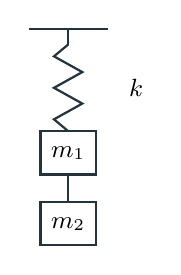
\begin{tikzpicture}
\draw[object] (-.5,3)--(.5,3);\draw[object] (0,3)--(0,2.8);
\draw[object] (0,2.8)--(-.18,2.65)--(.18,2.45)--(-.18,2.25)--(.18,2.05)--(-.18,1.85)--(0,1.7);
\filldraw[object,fill=white] (-.35,1.15) rectangle (.35,1.7);\node at (0,1.42) {$m_1$};\draw[object] (0,1.15)--(0,.8);\filldraw[object,fill=white] (-.35,.25) rectangle (.35,.8);\node at (0,.52) {$m_2$};\node[right] at (.65,2.25) {$k$};
\end{tikzpicture}
\figcaption{图 3.1\quad 撤去下挂物前的平衡状态。}
\end{minipage}\end{center}

\workarea

\clearpage

\pdfbookmark[3]{第 2 题 带摩擦水平弹簧振子的过原点条件}{c3-q2}

\section*{第 2 题\quad 带摩擦水平弹簧振子的过原点条件}\label{book-question-3-2}

\tagline{M-03-02}

水平轻弹簧一端固定，另一端连接质量为 $m$ 的小球，劲度系数为 $k$。小球在粗糙水平面上运动，静、动摩擦系数均为 $\mu$。弹簧原长位置为 $O$。从右侧 $OA=l_0$ 的 $A$ 点静止释放。
\begin{enumerate}\item 为使小球穿过 $O$ 且只穿过一次，$\mu$ 应取什么范围？以速度不为零并越到另一侧为“穿过”。\item 若还要求小球在左侧第一个转折点 $B$ 永久停住，$OB=l_1$ 的最大值是多少？\end{enumerate}

\begin{center}\begin{minipage}{\linewidth}\centering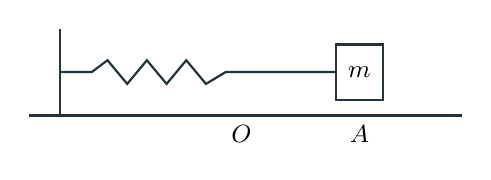
\begin{tikzpicture}
\draw[object] (-.4,0)--(5.1,0);\draw[object] (0,0)--(0,1.1);\draw[object] (0,.55)--(.4,.55)--(.6,.7)--(.85,.4)--(1.1,.7)--(1.35,.4)--(1.6,.7)--(1.85,.4)--(2.1,.55)--(3.5,.55);\filldraw[object,fill=white] (3.5,.2) rectangle (4.1,.9);\node at (3.8,.55) {$m$};\node[below] at (2.3,0) {$O$};\node[below] at (3.8,0) {$A$};
\end{tikzpicture}
\figcaption{图 3.2\quad 小球从伸长位置释放，摩擦始终反向于运动。}
\end{minipage}\end{center}

\workarea

\clearpage

\pdfbookmark[3]{第 3 题 斜面摩擦中动能等于势能的位置}{c3-q3}

\section*{第 3 题\quad 斜面摩擦中动能等于势能的位置}\label{book-question-3-3}

\tagline{M-03-03}

木块沿倾角 $\theta=30^\circ$ 的足够长斜面，以 $v_0=4.5\,\mathrm{m/s}$ 的初速度上滑。静、动摩擦系数均为 $\mu=0.35$。以初始位置为重力势能零点，求动能等于重力势能时相对初始位置的高度。取 $g=10\,\mathrm{m/s^2}$。

\begin{center}\begin{minipage}{\linewidth}\centering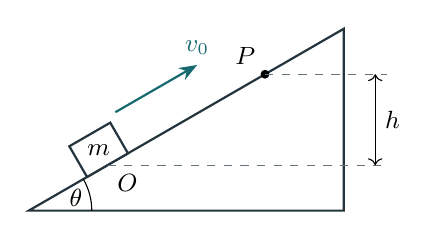
\begin{tikzpicture}
\draw[object] (0,0)--(4,2.309401)--(4,0)--cycle;
\filldraw[object,fill=white,rotate around={30:(1,.57735)}] (.7,.57735) rectangle (1.3,1.02735);
\node at (.8875,.772206) {$m$};\node[below right] at (1,.57735) {$O$};
\draw[motion] (1.1,1.25)--(2.13923,1.85) node[above] {$v_0$};
\draw (.8,0) arc(0:30:.8);\node at (.6,.16) {$\theta$};
\fill (3,1.732051) circle(1.6pt);\node[above left] at (3,1.732051) {$P$};
\draw[guide] (1,.57735)--(4.55,.57735);\draw[guide] (3,1.732051)--(4.55,1.732051);
\draw[<->] (4.4,.57735)--(4.4,1.732051) node[midway,right] {$h$};
\end{tikzpicture}
\figcaption{图 3.3\quad 从初始位置$O$量取竖直高度$h$，$P$表示上滑途中的位置。}
\end{minipage}\end{center}

\workarea

\clearpage

\pdfbookmark[3]{第 4 题 桌孔下落绳的速度与位置}{c3-q4}

\section*{第 4 题\quad 桌孔下落绳的速度与位置}\label{book-question-3-4}

\tagline{M-03-04}

均匀柔软、不可伸长的绳全长为 $l$，一部分平放在光滑水平桌面上，另一部分经过光滑小孔竖直下垂。初始下垂长度 $0<x_0<l$，整绳从静止下落。设桌上绳已经理顺，各段速率相同，小孔只改变运动方向。求绳速 $v(x)$ 及下端位置 $x(t)$，并说明适用时间。

\begin{center}\begin{minipage}{\linewidth}\centering\begin{tikzpicture}
\draw[object] (-2,1.6)--(-.12,1.6);\draw[object] (.12,1.6)--(1.7,1.6);\draw[traj] (-1.8,1.6)--(0,1.6)--(0,-.8);\node[above right] at (.15,1.6) {$O$};\draw[<->] (.7,-.8)--(.7,1.6) node[midway,right] {$x$};
\end{tikzpicture}
\figcaption{图 3.4\quad 向下量取下垂长度。}
\end{minipage}\end{center}

\workarea

\clearpage

\pdfbookmark[3]{第 5 题 单摆碰钉后的完整圆周与撞钉条件}{c3-q5}

\section*{第 5 题\quad 单摆碰钉后的完整圆周与撞钉条件}\label{book-question-3-5}

\tagline{M-03-05}

摆长为 $L$ 的单摆，从悬点 $O$ 左侧、与向下竖直方向夹角 $\alpha$ 处静止释放。右侧钉子 $P$ 满足 $OP=r<L$，$OP$ 与向下竖直方向夹角为 $\beta$，其中 $0<\beta<\alpha\leq90^\circ$。绳转到 $OP$ 方向后绕钉运动，绳与钉均理想光滑。求：\begin{enumerate}\item 完成绕钉圆周运动的最小释放角；\item 绳松弛后，小球沿抛物线直接击中钉子 $P$ 所需的释放角。若条件不能实现，应说明。\end{enumerate}

\begin{center}\begin{minipage}{\linewidth}\centering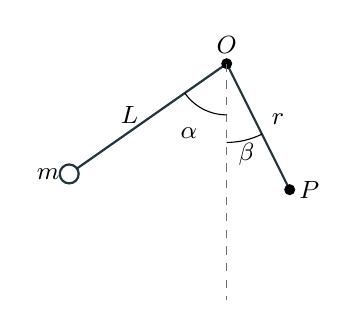
\begin{tikzpicture}
\coordinate(O)at(0,3);\coordinate(P)at(.8,1.4);\coordinate(A)at(-2,1.6);\draw[object] (A)--(O)--(.8,1.4);\fill(O)circle(2pt);\fill(P)circle(2pt);\filldraw[object,fill=white](A)circle(.12);\draw[guide](O)--(0,0);\node[above]at(O){$O$};\node[right]at(P){$P$};\node[left]at(A){$m$};\node[left]at(-1,2.35){$L$};\node[right]at(.45,2.3){$r$};\draw (0,2.35) arc(-90:-145:.65);\node at(-.48,2.12){$\alpha$};\draw (0,2) arc(-90:-63.435:1);\node at(.25,1.85){$\beta$};
\end{tikzpicture}
\figcaption{图 3.5\quad 绳碰钉后，运动半径变为 $a=L-r$。}
\end{minipage}\end{center}

\workarea

\clearpage

\pdfbookmark[3]{第 6 题 圆环双球下滑与悬线张力}{c3-q6}

\section*{第 6 题\quad 圆环双球下滑与悬线张力}\label{book-question-3-6}

\tagline{M-03-06}

质量 $M$、半径 $R$ 的竖直圆环，用轻细线悬挂。环上串着两个质量均为 $m$ 的光滑小球，从顶端以无限小扰动同时向两侧滑下。$\theta$ 从向上竖直半径量起。\begin{enumerate}\item 假设圆环不动，画出悬线张力 $T$ 随 $x=\cos\theta$ 的曲线，求最小值及对应角度。\item 求圆环可能上升的质量比阈值，画出阈值情形的曲线，并区分“张力为零”与“实际上升”。\end{enumerate}

\begin{center}\begin{minipage}{\linewidth}\centering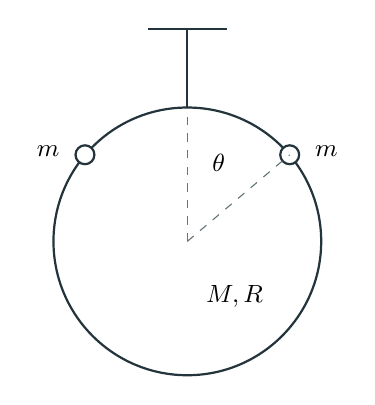
\begin{tikzpicture}
\draw[object](0,0)circle(1.7);\draw[object](0,1.7)--(0,2.7);\draw[object](-.5,2.7)--(.5,2.7);\filldraw[object,fill=white](1.3,1.1)circle(.12);\filldraw[object,fill=white](-1.3,1.1)circle(.12);\draw[guide](0,0)--(0,1.7);\draw[guide](0,0)--(1.3,1.1);\node at(.4,1){$\theta$};\node[right]at(1.5,1.15){$m$};\node[left]at(-1.5,1.15){$m$};\node at(.6,-.7){$M,R$};
\end{tikzpicture}
\figcaption{图 3.6\quad 小球串在环上，可承受环沿径向的推、拉作用。}
\end{minipage}\end{center}

\workarea

\clearpage

\pdfbookmark[3]{第 7 题 滑杆脱离约束后的落点}{c3-q7}

\section*{第 7 题\quad 滑杆脱离约束后的落点}\label{book-question-3-7}

\tagline{M-03-07}

长 $2r=20\,\mathrm{cm}$ 的理想轻杆，在中心 $C$ 固定质量为 $m$ 的质点。端点 $A$ 靠在光滑竖直墙上，端点 $B$ 支在光滑水平地面上。杆从近似竖直的位置由静止下滑，运动始终在同一竖直平面。按集中质量轻杆模型，求中心 $C$ 第一次触地时距墙角 $O$ 的水平距离。

\begin{center}\begin{minipage}{\linewidth}\centering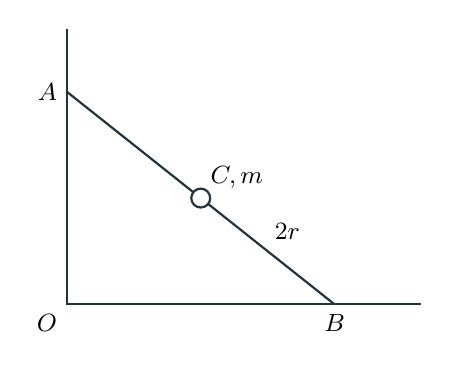
\begin{tikzpicture}
\draw[object](0,3.5)--(0,0)--(4.5,0);\draw[object](0,2.7)--(3.4,0);\filldraw[object,fill=white](1.7,1.35)circle(.12);\node[left]at(0,2.7){$A$};\node[below]at(3.4,0){$B$};\node[above right]at(1.7,1.35){$C,m$};\node[below left]at(0,0){$O$};\node[above]at(2.8,.7){$2r$};
\end{tikzpicture}
\figcaption{图 3.7\quad 两端保持接触时，杆中心沿半径 $r$ 的四分之一圆运动。}
\end{minipage}\end{center}

\workarea

\clearpage

\pdfbookmark[3]{第 8 题 轻杆小球跌落与触地速度}{c3-q8}

\section*{第 8 题\quad 轻杆小球跌落与触地速度}\label{book-question-3-8}

\tagline{M-03-08}

长 $L$ 的理想轻杆，上端固定一质量为 $m$ 的小球，下端支在粗糙水平地面。由近似竖直位置静止释放，球向右下落。设下端在失去地面支持前不滑动（静摩擦系数足够大），杆的质量可忽略。求球第一次碰地前速度的水平、竖直分量；竖直向上取正。

\begin{center}\begin{minipage}{\linewidth}\centering\begin{tikzpicture}
\draw[object](-.7,0)--(3,0);\draw[object](0,0)--(0,2.7);\filldraw[object,fill=white](0,2.7)circle(.14);\node[left]at(0,1.4){$L$};\node[below]at(0,0){$O$};\draw[motion](.3,2.5)--(1,2.3);\node[right]at(.2,2.7){$m$};
\end{tikzpicture}
\figcaption{图 3.8\quad 初始直立状态取无限小扰动的极限。}
\end{minipage}\end{center}

\workarea

\clearpage

\pdfbookmark[3]{第 9 题 绳绕钉运动与碰钉条件}{c3-q9}

\section*{第 9 题\quad 绳绕钉运动与碰钉条件}\label{book-question-3-9}

\tagline{M-03-09}

长 $2l$ 的理想细绳，一端固定在钉子 $A$，另一端系小球。小球初始位于 $A$ 右侧同一水平线上，以竖直向下初速度 $v_0$ 运动。钉子 $B$ 位于 $A$ 左侧，$AB=l$。绳转到 $B$ 后，小球绕 $B$ 上行。求小球直接碰到 $A$ 所需的最小初速，允许松绳后以抛体轨迹命中。

\begin{center}\begin{minipage}{\linewidth}\centering\begin{tikzpicture}
\fill(0,0)circle(2pt);\fill(-1.5,0)circle(2pt);\draw[object](0,0)--(3,0);\filldraw[object,fill=white](3,0)circle(.1);\node[above]at(0,0){$A$};\node[above]at(-1.5,0){$B$};\draw[motion](3,0)--(3,-1)node[right]{$v_0$};\draw[guide](3,0)arc(0:-180:3);\draw[<->](-1.5,.65)--(0,.65)node[midway,above]{$l$};
\end{tikzpicture}
\figcaption{图 3.9\quad 先绕 $A$ 经过下半圆，再绕 $B$ 向上运动。}
\end{minipage}\end{center}

\workarea

\clearpage

\pdfbookmark[3]{第 10 题 引力追及中的最大间距}{c3-q10}

\section*{第 10 题\quad 引力追及中的最大间距}\label{book-question-3-10}

\tagline{M-03-10}

惯性系 $S$ 中，质量分别为 $m_1,m_2$ 的质点 $A,B$ 以万有引力相互吸引。起初 $A$ 静止，间距 $l_0$；$B$ 沿连线远离 $A$，速度 $v_0<\sqrt{2Gm_2/l_0}$。外力 $F$ 始终作用于 $B$，使其速度保持 $v_0$。求两点最大间距及达到该间距前外力在 $S$ 中所做的功。

\begin{center}\begin{minipage}{\linewidth}\centering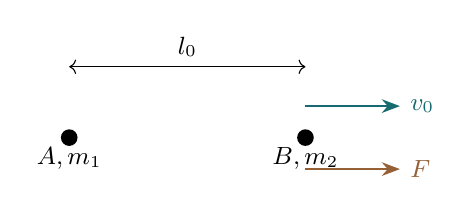
\begin{tikzpicture}
\fill(0,0)circle(3pt);\fill(3,0)circle(3pt);\node[below]at(0,0){$A,m_1$};\node[below]at(3,0){$B,m_2$};\draw[motion](3,.4)--(4.2,.4)node[right]{$v_0$};\draw[force](3,-.4)--(4.2,-.4)node[right]{$F$};\draw[<->](0,.9)--(3,.9)node[midway,above]{$l_0$};
\end{tikzpicture}
\figcaption{图 3.10\quad $F$ 抵消 $B$ 所受引力，$A$ 则不断加速。}
\end{minipage}\end{center}

\workarea

\clearpage

\pdfbookmark[3]{第 11 题 地球直通隧道中的运动}{c3-q11}

\section*{第 11 题\quad 地球直通隧道中的运动}\label{book-question-3-11}

\tagline{M-03-11}

将地球看作半径 $R$、密度均匀且不自转的球体，地表重力加速度为 $g$。在地表两点 $A,B$ 间开一直通光滑隧道，长度为 $L$。小球从 $A$ 静止释放，忽略空气及其他阻力。求最大速率和首次从 $A$ 到 $B$ 的时间。

\begin{center}\begin{minipage}{\linewidth}\centering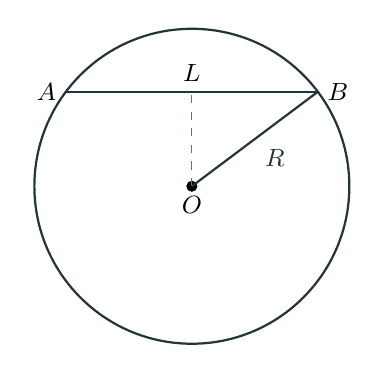
\begin{tikzpicture}
\draw[object](0,0)circle(2);\draw[object](-1.6,1.2)--(1.6,1.2);\fill(0,0)circle(2pt);\node[below]at(0,0){$O$};\node[left]at(-1.6,1.2){$A$};\node[right]at(1.6,1.2){$B$};\draw[guide](0,0)--(0,1.2);\draw[object](0,0)--(1.6,1.2)node[midway,below right]{$R$};\node[above]at(0,1.2){$L$};
\end{tikzpicture}
\figcaption{图 3.11\quad 隧道方向的引力分量指向隧道中点。}
\end{minipage}\end{center}

\workarea

\clearpage

\pdfbookmark[3]{第 12 题 旋转杆上双弹簧小球}{c3-q12}

\section*{第 12 题\quad 旋转杆上双弹簧小球}\label{book-question-3-12}

\tagline{M-03-12}

两个质量均为 $m$ 的小球串在理想光滑轻杆上，杆绕固定点 $O$ 在水平面内转动。两根相同轻弹簧依次连接 $O$、内球、外球，劲度系数均为 $k$，原长均为 $l_0$。角速度由零无限缓慢增加到 $\omega$，径向瞬态振动可忽略。求外力所做的功、两弹簧长度之比，以及这一准静态分支允许的 $\omega$ 范围。

\begin{center}\begin{minipage}{\linewidth}\centering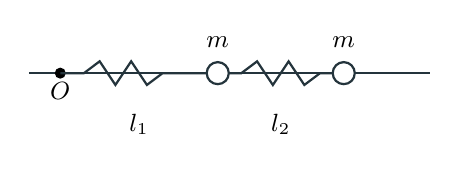
\begin{tikzpicture}
\draw[object](-.4,.2)--(4.7,.2);\fill(0,.2)circle(2pt);\node[below]at(0,.2){$O$};\draw[object](0,.2)--(.3,.2)--(.5,.35)--(.7,.05)--(.9,.35)--(1.1,.05)--(1.3,.2)--(2,.2);\draw[object](2,.2)--(2.3,.2)--(2.5,.35)--(2.7,.05)--(2.9,.35)--(3.1,.05)--(3.3,.2)--(3.6,.2);\filldraw[object,fill=white](2,.2)circle(.14);\filldraw[object,fill=white](3.6,.2)circle(.14);\node[above]at(2,.4){$m$};\node[above]at(3.6,.4){$m$};\node[below]at(1,-.2){$l_1$};\node[below]at(2.8,-.2){$l_2$};
\end{tikzpicture}
\figcaption{图 3.12\quad 外球到转轴的距离为 $l_1+l_2$。}
\end{minipage}\end{center}

\workarea

\clearpage

\pdfbookmark[3]{第 13 题 旋转圆环中的平衡稳定性}{c3-q13}

\section*{第 13 题\quad 旋转圆环中的平衡稳定性}\label{book-question-3-13}

\tagline{M-03-13}

半径为 $R$ 的光滑竖直圆环，绕其竖直直径以恒定角速度 $\omega$ 转动。质量为 $m$ 的小球串在环上。用从最低点向右量起的有符号角 $\theta$ 表示位置。求相对圆环的平衡位置并讨论稳定性，包含临界角速度的情形。

\begin{center}\begin{minipage}{\linewidth}\centering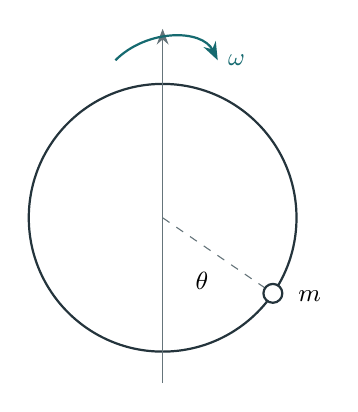
\begin{tikzpicture}
\draw[object](0,0)circle(1.7);\draw[axis](0,-2.1)--(0,2.4);\draw[guide](0,0)--(1.4,-.96);\filldraw[object,fill=white](1.4,-.96)circle(.12);\node[right]at(1.6,-1){$m$};\node at(.5,-.8){$\theta$};\draw[motion](-.6,2)..controls(-.2,2.4)and(.5,2.4)..(.7,2)node[right]{$\omega$};
\end{tikzpicture}
\figcaption{图 3.13\quad 左右对称的非最低点平衡须成对出现。}
\end{minipage}\end{center}

\workarea

\clearpage

\pdfbookmark[3]{第 14 题 弹性小球与移动墙壁}{c3-q14}

\section*{第 14 题\quad 弹性小球与移动墙壁}\label{book-question-3-14}

\tagline{M-03-14}

质量为 $m$ 的小球在相距 $l$ 的两平行墙壁间，以垂直于墙壁的初速 $v_0$ 往返。墙质量远大于球，碰撞完全弹性，忽略其他作用。\begin{enumerate}\item 两墙固定时，求每壁所受平均力。\item 左壁以 $V\ll v_0$ 缓慢右移，证明在准静态极限中，外力对左壁所做的功等于小球动能增加量。\end{enumerate}

\begin{center}\begin{minipage}{\linewidth}\centering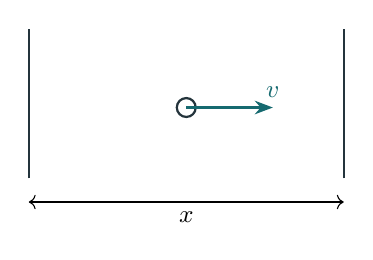
\begin{tikzpicture}
\draw[object](0,-.5)--(0,1.4);\draw[object](4,-.5)--(4,1.4);\filldraw[object,fill=white](2,.4)circle(.12);\draw[motion](2,.4)--(3.1,.4)node[above]{$v$};\draw[<->](0,-.8)--(4,-.8)node[midway,below]{$x$};
\end{tikzpicture}
\figcaption{图 3.14\quad 第二问中，壁距从 $l$ 缩短到 $x$。}
\end{minipage}\end{center}

\workarea

\clearpage

\pdfbookmark[3]{第 15 题 三质点绳系冲量}{c3-q15}

\section*{第 15 题\quad 三质点绳系冲量}\label{book-question-3-15}

\tagline{M-03-15}

光滑水平面上，静止质点 $A,B,C$ 的质量分别为 $m_1,m_2,m_3$，用两段拉直的理想细绳相连。$\alpha$ 是 $A\to B$ 与 $B\to C$ 两方向的夹角，$0\leq\alpha<90^\circ$。沿 $B\to C$ 方向对 $C$ 施加冲量 $I$。求 $A$ 刚开始运动的速率。

\begin{center}\begin{minipage}{\linewidth}\centering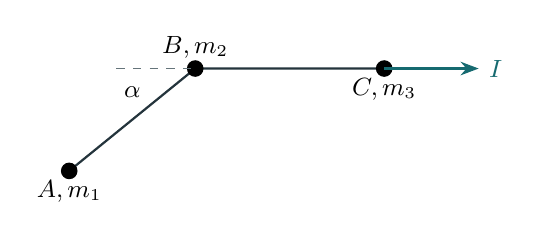
\begin{tikzpicture}
\coordinate(A)at(-1.6,-1.3);\coordinate(B)at(0,0);\coordinate(C)at(2.4,0);\draw[object](A)--(B)--(C);\fill(A)circle(3pt);\fill(B)circle(3pt);\fill(C)circle(3pt);\node[below]at(A){$A,m_1$};\node[above]at(B){$B,m_2$};\node[below]at(C){$C,m_3$};\draw[motion](C)--(3.6,0)node[right]{$I$};\draw[guide](-1,0)--(B);\node at(-.8,-.3){$\alpha$};
\end{tikzpicture}
\figcaption{图 3.15\quad 俯视图；夹角按两条有向绳段的方向定义。}
\end{minipage}\end{center}

\workarea

\clearpage

\pdfbookmark[3]{第 16 题 炮弹最高点爆炸}{c3-q16}

\section*{第 16 题\quad 炮弹最高点爆炸}\label{book-question-3-16}

\tagline{M-03-16}

炮弹从地面发射，在最高点炸成质量相等的两块。最高点高 $h=19.6\,\mathrm m$，其正下方距发射点 $S_1=1000\,\mathrm m$。第一块在爆炸后 $1.00\,\mathrm s$ 落到该正下方点。忽略空气阻力，取 $g=9.8\,\mathrm{m/s^2}$，求第二块落地点距发射点的水平距离。

\begin{center}\begin{minipage}{\linewidth}\centering\begin{tikzpicture}
\draw[object](-.3,0)--(6,0);\draw[traj](0,0)..controls(.5,1.8)and(1.5,2.4)..(2.2,2.4);\draw[guide](2.2,2.4)--(2.2,0);\fill(2.2,2.4)circle(3pt);\node[above]at(2.2,2.4){爆炸点};\node[below]at(0,0){$O$};\node[below]at(2.2,0){$S_1$};\draw[<->](3,0)--(3,2.4)node[midway,right]{$h$};
\end{tikzpicture}
\figcaption{图 3.16\quad 图示不按水平与竖直距离的实际比例。}
\end{minipage}\end{center}

\workarea

\clearpage

\pdfbookmark[3]{第 17 题 平板车上多人跳离}{c3-q17}

\section*{第 17 题\quad 平板车上多人跳离}\label{book-question-3-17}

\tagline{M-03-17}

光滑水平地面上，静止平板车质量为 $M$，载有 $N$ 人，每人质量为 $m$。每人向车后跳离，相对于该次跳离后车的速度大小均为 $u$。比较 $N$ 人同时跳离与逐个跳离后，车所得动能的大小。

\begin{center}\begin{minipage}{\linewidth}\centering\begin{tikzpicture}
\draw[object](0,.3)rectangle(4,.6);\draw[object](.6,.15)circle(.15);\draw[object](3.4,.15)circle(.15);\draw[object](-.5,0)--(5,0);\foreach\x in {.8,2,3.2}{\filldraw[object,fill=white](\x,1.1)circle(.15);\draw[object](\x,.95)--(\x,.6);}\node at(2,.43){$M$};\node[above]at(2,1.45){$N$ 人，每人 $m$};
\end{tikzpicture}
\figcaption{图 3.17\quad 向右取车前进的正方向。}
\end{minipage}\end{center}

\workarea

\clearpage

\pdfbookmark[3]{第 18 题 下滑木块中支持力做功}{c3-q18}

\section*{第 18 题\quad 下滑木块中支持力做功}\label{book-question-3-18}

\tagline{M-03-18}

质量 $M$、倾角 $\theta$ 的斜面体放在光滑水平地面上，质量 $m$ 的木块从斜面顶端高 $h$ 处静止滑至底端。块与斜面之间也光滑。以地面为参考系，求斜面支持力对木块做的功。

\begin{center}\begin{minipage}{\linewidth}\centering\begin{tikzpicture}
\draw[object](0,0)--(4,0)--(0,2.2)--cycle;\filldraw[object,fill=white,rotate around={-28.81:(.4,1.98)}](.1,1.98)rectangle(.7,2.4);\node at(1.4,.55){$M$};\node[above]at(.45,2.4){$m$};\draw[<->](-.5,0)--(-.5,2.2)node[midway,left]{$h$};\draw[object](-1,0)--(5,0);\node at(3.15,.25){$\theta$};
\end{tikzpicture}
\figcaption{图 3.18\quad 木块相对斜面向右下滑，斜面向左移动。}
\end{minipage}\end{center}

\workarea

\clearpage

\pdfbookmark[3]{第 19 题 半圆槽中小球与木块}{c3-q19}

\section*{第 19 题\quad 半圆槽中小球与木块}\label{book-question-3-19}

\tagline{M-03-19}

质量 $M$ 的木块放在光滑水平地面上，其上部有半径 $R$ 的光滑半圆凹槽。质量 $m$ 的小球从凹槽右侧最高边缘静止下滑。$\theta$ 为槽心到球的半径与向下竖直方向的夹角，$0\leq\theta\leq\pi/2$。求球的地面速率 $v$、木块向右速率 $V$、球相对槽速率 $w$ 的位置函数；再求球在最低点对槽的压力。

\begin{center}\begin{minipage}{\linewidth}\centering\begin{tikzpicture}
\draw[object](-2,1.7)--(-2,-.35)--(2,-.35)--(2,1.7);\draw[object](-1.7,1.7)arc(180:360:1.7);\draw[object](-2,1.7)--(-1.7,1.7);\draw[object](1.7,1.7)--(2,1.7);\filldraw[object,fill=white](1.7,1.7)circle(.1);\node[right]at(1.9,1.8){$m$};\node at(0,-.2){$M$};\draw[guide](0,1.7)--(0,0);\node[left]at(0,.9){$R$};
\end{tikzpicture}
\figcaption{图 3.19\quad 球从右缘沿凹槽向左下滑。}
\end{minipage}\end{center}

\workarea

\clearpage

\pdfbookmark[3]{第 20 题 非弹性碰撞后弹簧带起木块}{c3-q20}

\section*{第 20 题\quad 非弹性碰撞后弹簧带起木块}\label{book-question-3-20}

\tagline{M-03-20}

地面上的木块 $m_3$ 通过劲度系数 $k$ 的竖直轻弹簧连接上方木块 $m_2$，初始静止平衡。小球 $m_1$ 从距 $m_2$ 高 $h$ 处静止落下，与 $m_2$ 完全非弹性碰撞并粘住。求使反弹过程中弹簧拉力恰好达到 $m_3g$（离地临界）的最小 $h$。

\begin{center}\begin{minipage}{\linewidth}\centering\begin{tikzpicture}
\draw[object](-1,0)--(1,0);\filldraw[object,fill=white](-.5,0)rectangle(.5,.5);\node at(0,.25){$m_3$};\draw[object](0,.5)--(0,.7)--(-.2,.85)--(.2,1.05)--(-.2,1.25)--(.2,1.45)--(0,1.6);\filldraw[object,fill=white](-.5,1.6)rectangle(.5,2.1);\node at(0,1.85){$m_2$};\filldraw[object,fill=white](0,3.2)circle(.12);\node[right]at(.2,3.2){$m_1$};\draw[<->](1,2.1)--(1,3.2)node[midway,right]{$h$};
\end{tikzpicture}
\figcaption{图 3.20\quad 初始弹簧压缩量为 $m_2g/k$。}
\end{minipage}\end{center}

\workarea

\clearpage

\pdfbookmark[3]{第 21 题 滑块弹簧与断绳条件}{c3-q21}

\section*{第 21 题\quad 滑块弹簧与断绳条件}\label{book-question-3-21}

\tagline{M-03-21}

质量 $M$ 的长滑块静置于光滑水平面，右端用最大承受拉力为 $T_0$ 的理想绳系在墙上，左端固定劲度系数 $k$ 的轻弹簧。质量 $m$ 的小物以向左初速 $v_0$ 在滑块上无摩擦运动，压缩弹簧。约定绳张力达到 $T_0$ 即断裂，断裂本身不消耗能量。求：\begin{enumerate}\item 断绳的最小 $v_0$；\item 断绳后滑块的最大加速度；\item 小物脱离弹簧后，相对桌面的速度为零的条件。\end{enumerate}

\begin{center}\begin{minipage}{\linewidth}\centering\begin{tikzpicture}
\draw[object](0,0)rectangle(4,.35);\draw[object](0,.35)--(0,1.1);\draw[object](0,.7)--(.3,.7)--(.5,.85)--(.7,.55)--(.9,.85)--(1.1,.55)--(1.3,.7)--(1.8,.7);\filldraw[object,fill=white](2.8,.35)rectangle(3.4,.9);\node at(3.1,.62){$m$};\node at(2,.17){$M$};\draw[object](4,.17)--(5.2,.17);\draw[object](5.2,-.2)--(5.2,1.2);\node[above]at(4.6,.17){$T_0$};\draw[motion](3.4,1.3)--(2.3,1.3)node[left]{$v_0$};
\end{tikzpicture}
\figcaption{图 3.21\quad 弹簧接触只在压缩阶段存在，小物反弹到原长后离开。}
\end{minipage}\end{center}

\workarea

\clearpage

\pdfbookmark[3]{第 22 题 两球与墙的碰撞次数}{c3-q22}

\section*{第 22 题\quad 两球与墙的碰撞次数}\label{book-question-3-22}

\tagline{M-03-22}

两小球在光滑水平面上沿同一直线运动，质量为 $m_1,m_2$。球 1 以初速 $u>0$ 向右，球 2 起初静止，球 2 右侧有固定弹性墙。球间、球墙的碰撞均完全弹性。求使两球彼此恰好碰撞两次的质量比范围；球墙碰撞不计入“两次”。

\begin{center}\begin{minipage}{\linewidth}\centering\begin{tikzpicture}
\draw[object](4,-.5)--(4,1.4);\filldraw[object,fill=white](0,.3)circle(.2);\filldraw[object,fill=white](2,.3)circle(.28);\node[below]at(0,0){$1,m_1$};\node[below]at(2,-.1){$2,m_2$};\draw[motion](0,.8)--(1.2,.8)node[above]{$u$};
\end{tikzpicture}
\figcaption{图 3.22\quad 球 2 始终位于球 1 与右墙之间。}
\end{minipage}\end{center}

\workarea

\clearpage

\pdfbookmark[3]{第 23 题 三球铰链杆释放}{c3-q23}

\section*{第 23 题\quad 三球铰链杆释放}\label{book-question-3-23}

\tagline{M-03-23}

两根长度均为 $l$ 的理想轻杆，在一端用质量 $m$ 的球形铰链连接，另一端分别装质量 $m$ 和 $2m$ 的小球。两端球在光滑水平桌面上，初始两杆近似并拢且竖直，铰链在上，从静止释放后两端球向两侧分开。三球和两杆始终在同一竖直平面。求铰链球碰桌前的速率，以及两杆夹角为 $90^\circ$ 时 $2m$ 球的速率。

\begin{center}\begin{minipage}{\linewidth}\centering\begin{tikzpicture}
\coordinate(A)at(-1.7,0);\coordinate(B)at(1.7,0);\coordinate(C)at(0,1.7);\draw[object](A)--(C)--(B);\foreach\p in {A,B,C}{\filldraw[object,fill=white](\p)circle(.12);}\draw[object](-2.5,0)--(2.5,0);\node[below]at(A){$m$};\node[below]at(B){$2m$};\node[above]at(C){$m$};\node[left]at(-.9,.9){$l$};\node[right]at(.9,.9){$l$};
\end{tikzpicture}
\figcaption{图 3.23\quad 图示中间状态；两端等高，两杆始终关于铰链所在竖直线几何对称。}
\end{minipage}\end{center}

\workarea

\clearpage

\pdfbookmark[3]{第 24 题 小球反复弹跳总时间}{c3-q24}

\section*{第 24 题\quad 小球反复弹跳总时间}\label{book-question-3-24}

\tagline{M-03-24}

小球从高 $h$ 处静止下落，与水平地面的恢复系数为 $e$。忽略空气阻力及每次碰撞的持续时间。求从释放到无限次弹跳时间累积终点的总时间，并讨论 $0\leq e\leq1$。

\begin{center}\begin{minipage}{\linewidth}\centering\begin{tikzpicture}
\draw[object](-.5,0)--(5,0);\filldraw[object,fill=white](0,2.6)circle(.1);\draw[motion](0,2.4)--(0,1.5);\draw[<->](-.6,0)--(-.6,2.6)node[midway,left]{$h$};\draw[traj](0,0)..controls(.4,2.3)and(.9,2.3)..(1.3,0)..controls(1.6,1.3)and(2,1.3)..(2.4,0)..controls(2.6,.65)and(2.9,.65)..(3.2,0);
\end{tikzpicture}
\figcaption{图 3.24\quad 弹跳次数以展开示意表示，小球实际始终竖直运动。}
\end{minipage}\end{center}

\workarea

\clearpage

\pdfbookmark[3]{第 25 题 台阶逐级弹跳}{c3-q25}

\section*{第 25 题\quad 台阶逐级弹跳}\label{book-question-3-25}

\tagline{M-03-25}

台阶每级宽、高均为 $l$，水平踏面光滑。小球逐级向下弹跳，每次反弹后相对本级踏面的最大高度均为 $H$，落点在各级踏面的相同相对位置。小球与踏面的恢复系数为 $0<e<1$，不碰立面。求小球的水平速率及 $H$。

\begin{center}\begin{minipage}{\linewidth}\centering\begin{tikzpicture}
\draw[object] (-.3,3.6)--(1.2,3.6)--(1.2,2.4)--(2.4,2.4)--(2.4,1.2)--(3.6,1.2)--(3.6,0)--(4.8,0);
\foreach \xA/\yA in {.5/3.6,1.7/2.4,2.9/1.2}{
 \draw[traj,domain=0:1,samples=60] plot({\xA+1.2*\x},{\yA+1.2*(2*\x-3*\x^2)});
 \fill (\xA,\yA) circle(1.6pt);}
\draw[<->] (-.65,2.4)--(-.65,3.6) node[midway,left] {$l$};
\draw[<->] (1.2,2.12)--(2.4,2.12) node[midway,below] {$l$};
\end{tikzpicture}
\figcaption{图3.25\quad 等宽等高台阶；示意取$e=1/2$，相邻落点水平、竖直距离均为$l$。}
\end{minipage}\end{center}

\workarea

\clearpage

\pdfbookmark[3]{第 26 题 固定斜面碰撞反弹}{c3-q26}

\section*{第 26 题\quad 固定斜面碰撞反弹}\label{book-question-3-26}

\tagline{M-03-26}

小球在固定光滑斜面上 $O$ 点正上方 $h=1.60\,\mathrm m$ 处静止释放。斜面向右下方倾斜，倾角 $\theta=15^\circ$，恢复系数 $e=0.60$。忽略空气阻力。求碰后最大上升高度（相对 $O$）、再次撞到斜面的点 $P$ 与 $O$ 的沿面距离，以及碰撞造成的机械能损失百分数。取 $g=9.8\,\mathrm{m/s^2}$。

\begin{center}\begin{minipage}{\linewidth}\centering\begin{tikzpicture}
\draw[object](-1,.267949)--(4,-1.071797);\coordinate(O)at(0,0);\filldraw[object,fill=white](0,2.4)circle(.1);\draw[motion](0,2.2)--(0,1.3)node[right]{$u$};\node[below left]at(O){$O$};\draw[guide](-.5,0)--(1.6,0);\draw (.8,0) arc(0:-15:.8);\node at(.95,-.12){$\theta$};\draw[<->](-.6,0)--(-.6,2.4)node[midway,left]{$h$};
\end{tikzpicture}
\figcaption{图 3.26\quad 碰撞瞬间法向反弹、切向速度不变。}
\end{minipage}\end{center}

\workarea

\clearpage

\pdfbookmark[3]{第 27 题 可动斜面上的斜碰}{c3-q27}

\section*{第 27 题\quad 可动斜面上的斜碰}\label{book-question-3-27}

\tagline{M-03-27}

质量 $M=2m$ 的斜面体静止在光滑水平桌面上，斜面向右下倾 $\theta=15^\circ$。小球质量为 $m$，从原碰撞点正上方 $h=1.60\,\mathrm m$ 处静止落下，碰撞点距桌面 $H=1.00\,\mathrm m$。斜面光滑，法向相对速度的恢复系数 $e=0.60$，斜面从该点向右延伸至桌面。求碰后两物体的地面速度、小球最高点相对原碰撞点的高度，并判断下一次落在斜面还是桌面。取 $g=9.8\,\mathrm{m/s^2}$。

\begin{center}\begin{minipage}{\linewidth}\centering\begin{tikzpicture}[scale=1.3]
\draw[object](-.8,0)--(3.732051,0)--(-.8,1.214359)--cycle;
\draw[object](-1.5,0)--(4.3,0);\node at(1,.3){$M=2m$};
\filldraw[object,fill=white](0,2.6)circle(.09);\node[left]at(-.13,2.6){$m$};
\draw[motion](0,2.35)--(0,1.6)node[right]{$u$};
\fill(0,1)circle(2pt);\node[above left]at(0,1){$O$};
\draw[guide](0,1)--(1,1);\draw[guide](0,2.6)--(.6,2.6);
\draw[<->](-1.25,0)--(-1.25,1)node[midway,left]{$H$};
\draw[<->](.55,1)--(.55,2.6)node[midway,right]{$h$};
\draw (3.032051,0) arc(180:165:.7);\node at(2.9,.12){$\theta$};
\end{tikzpicture}
\figcaption{图3.27\quad 按$15^\circ$绘制斜面；$O$距桌面$H$，球从$O$上方$h$处释放。}
\end{minipage}\end{center}

\workarea

\clearpage

\pdfbookmark[3]{第 28 题 相对平板的反射定律}{c3-q28}

\section*{第 28 题\quad 相对平板的反射定律}\label{book-question-3-28}

\tagline{M-03-28}

光滑水平桌面上，小球与光滑平板作完全弹性碰撞。平板允许自由平移，不发生转动；碰前可处于任意匀速平移状态。证明：分别用碰前、碰后小球相对平板的速度定义入射角和反射角时，两角相等。角度均从接触面法线量起。

\begin{center}\begin{minipage}{\linewidth}\centering\begin{tikzpicture}
\draw[object](-2,0)--(2,0);\draw[guide](0,-1.6)--(0,1.8);\draw[motion](-1.3,1.3)--(0,0)node[midway,left]{$\vect w_{\mathrm{in}}$};\draw[motion](0,0)--(1.3,1.3)node[midway,right]{$\vect w_{\mathrm{out}}$};\node[below]at(1.7,0){平板};
\end{tikzpicture}
\figcaption{图 3.28\quad 俯视图；两箭头代表相对平板的速度。}
\end{minipage}\end{center}

\workarea

\clearpage

\pdfbookmark[3]{第 29 题 小球在可动圆环内反射}{c3-q29}

\section*{第 29 题\quad 小球在可动圆环内反射}\label{book-question-3-29}

\tagline{M-03-29}

质量 $M$、半径 $R$ 的均匀光滑圆环静止放在光滑水平桌面上。质点小球质量为 $m$，以地面速度 $v$ 从环上小孔 $H$ 入内，与环内壁完全弹性碰撞 $N\geq1$ 次后，在相对圆环的轨迹上绕一周，再恰好经 $H$ 离开。求入射方向及球、环的出射后地面速度。

\begin{center}\begin{minipage}{\linewidth}\centering\begin{tikzpicture}
\draw[object](0,0)circle(1.8);
\coordinate(H)at(1.8,0);\fill(H)circle(2pt)node[above right]{$H$};
\draw[guide](0,0)--(H);\node[below]at(0,0){$O$};
\draw[motion](2.8,-.5)--(H)node[midway,below]{$v$};
\draw[guide](H)--(.7,.55);
\draw(1.2,0)arc[start angle=180,end angle=153.43495,radius=.6];
\node at(.95,.20){$\theta$};\node at(-.4,2.2){俯视图};
\end{tikzpicture}
\figcaption{图 3.29\quad 入射角 $\theta$ 从 $H\to O$ 的内法线量起。}
\end{minipage}\end{center}

\workarea

\clearpage

\pdfbookmark[3]{第 30 题 三质点万有引力相对平衡}{c3-q30}

\section*{第 30 题\quad 三质点万有引力相对平衡}\label{book-question-3-30}

\tagline{M-03-30}

质量分别为 $m_1,m_2,m_3$ 的三质点，只通过万有引力相互作用，以共同角速度 $\omega$ 绕通过质心、垂直于它们所在平面的轴转动。求保持相对位置不变的条件。先讨论三点不共线的情形，再说明共线情形是否可能。

\begin{center}\begin{minipage}{\linewidth}\centering\begin{tikzpicture}
\coordinate(A)at(0,0);\coordinate(B)at(3,0);\coordinate(D)at(1.5,2.598);\draw[object](A)--(B)--(D)--cycle;\foreach\p/\lab in {A/1,B/2,D/3}{\fill(\p)circle(3pt);\node[above right]at(\p){$m_\lab$};}\fill(1.2,.8)circle(2pt);\node[right]at(1.2,.8){$C$};\node[below]at(1.5,0){$a$};
\end{tikzpicture}
\figcaption{图 3.30\quad 质心一般不在几何中心；等边图示对应非共线解。}
\end{minipage}\end{center}

\workarea

\clearpage

\pdfbookmark[3]{第 31 题 等功跳车的动能比较}{c3-q31}

\section*{第 31 题\quad 等功跳车的动能比较}\label{book-question-3-31}

\tagline{M-03-31}

静止平板车质量为 $M$，光滑地面上的车载 $N$ 人，每人质量为 $m$。每人以相同的功 $w$ 向车后跳离，假设这些功都转化为车和人的平动动能，不计耗散及转动。怎样安排跳法能使车最终动能最大？求该最大值。

\begin{center}\begin{minipage}{\linewidth}\centering\begin{tikzpicture}
\draw[object](0,.3)rectangle(4,.6);\draw[object](.6,.15)circle(.15);\draw[object](3.4,.15)circle(.15);\draw[object](-.5,0)--(5,0);\foreach\x in {.8,2,3.2}{\filldraw[object,fill=white](\x,1.1)circle(.15);\draw[object](\x,.95)--(\x,.6);}\node at(2,.43){$M$};\node[above]at(2,1.45){$N$ 人，每人 $m$};
\end{tikzpicture}
\figcaption{图 3.31\quad 本题固定每人的功，区别于第 17 题固定相对跳速。}
\end{minipage}\end{center}

\workarea

\clearpage

\pdfbookmark[3]{第 32 题 子弹射入弹簧连接木块}{c3-q32}

\section*{第 32 题\quad 子弹射入弹簧连接木块}\label{book-question-3-32}

\tagline{M-03-32}

光滑水平面上，质量 $m_1,m_2$ 的木块用劲度系数 $k$ 的轻弹簧相连，起初静止且弹簧为原长。子弹质量 $m$，以水平向右初速 $v_0$ 射入 $m_1$ 并嵌住，射入时间极短。求随后弹簧的最大压缩量，以及 $m_2$ 相对地面的最大、最小速度。

\begin{center}\begin{minipage}{\linewidth}\centering\begin{tikzpicture}
\filldraw[object,fill=white](0,0)rectangle(.8,.7);\filldraw[object,fill=white](3,0)rectangle(3.8,.7);\node at(.4,.35){$m_1$};\node at(3.4,.35){$m_2$};\draw[object](.8,.35)--(1.2,.35)--(1.4,.5)--(1.6,.2)--(1.8,.5)--(2,.2)--(2.2,.5)--(2.4,.2)--(2.6,.35)--(3,.35);\fill(-1.4,.35)circle(2pt);\draw[motion](-1.4,.35)--(-.3,.35)node[midway,above]{$m,v_0$};
\end{tikzpicture}
\figcaption{图 3.32\quad 碰撞瞬间弹簧长度来不及改变，第二块尚无速度。}
\end{minipage}\end{center}

\workarea

\clearpage

\pdfbookmark[3]{第 33 题 箱中滑块多次碰撞}{c3-q33}

\section*{第 33 题\quad 箱中滑块多次碰撞}\label{book-question-3-33}

\tagline{M-03-33}

质量为 $m$ 的箱子起初静止于光滑水平地面，箱内底面光滑，有质量同为 $m$ 的质点滑块。滑块以水平初速 $v_0$ 向右运动，与两内壁反复碰撞，恢复系数 $e=2^{-1/4}$，碰撞时间可略。\begin{enumerate}\item 最多碰撞几次，系统总动能损失仍不大于初始动能的 $40\%$？\item 箱内宽度为 $L$，滑块初始距左壁 $x_0$，求从开始到完成上述次数的碰撞时箱子的平均速度，并给出 $x_0=0$ 的结果。\end{enumerate}

\begin{center}\begin{minipage}{\linewidth}\centering\begin{tikzpicture}
\draw[object](0,0)rectangle(4,1.3);\filldraw[object,fill=white](.1,.1)rectangle(.7,.7);\node at(.4,.4){$m$};\node[above]at(2,1.3){箱子质量 $m$};\draw[motion](.8,.6)--(1.9,.6)node[above]{$v_0$};\draw[<->](0,-.4)--(4,-.4)node[midway,below]{$L$};
\end{tikzpicture}
\figcaption{图 3.33\quad 图示滑块从左壁附近向右；第二问保留一般初始位置。}
\end{minipage}\end{center}

\workarea

\clearpage

\pdfbookmark[3]{第 34 题 核反应阈能}{c3-q34}

\section*{第 34 题\quad 核反应阈能}\label{book-question-3-34}

\tagline{M-03-34}

动能为 $E_0$ 的 $^{4}\mathrm{He}$ 核轰击静止的 $^{7}\mathrm{Li}$ 核，先形成复合核，再分裂为 $^{10}\mathrm B$ 和中子 $^{1}\mathrm n$。反应吸收能量 $Q=2.8\,\mathrm{MeV}$。采用非相对论近似，各核惯性质量按质量数之比 $4:7:10:1$ 取值，忽略质量亏损对平动质量的修正。求反应所需最小 $E_0$，及阈值处中子的实验室动能。

\begin{center}\begin{minipage}{\linewidth}\centering\begin{tikzpicture}
\node[draw,circle]at(0,0){$^4\mathrm{He}$};\node[draw,circle]at(3,0){$^7\mathrm{Li}$};\draw[motion](.6,0)--(2.3,0)node[midway,above]{$E_0$};\node at(3,-1){靶核静止};\node[align=left]at(6,0){$^{10}\mathrm B+{}^1\mathrm n$\\吸收 $Q$};
\end{tikzpicture}
\figcaption{图 3.34\quad 阈值由可用于相对运动的动能决定。}
\end{minipage}\end{center}

\workarea

\clearpage

\pdfbookmark[3]{第 35 题 变质量物体方程}{c3-q35}

\section*{第 35 题\quad 变质量物体方程}\label{book-question-3-35}

\tagline{M-03-35}

一主体作直线运动，质量 $M(t)$、地面速度 $v(t)$ 随时间变化。以 $u$ 表示加入质量进入前，或流出质量离开后的地面速度，$F$ 为主体所受合外力。用短时间内质量固定的扩展系统证明
\[
M\frac{\dd v}{\dd t}=(u-v)\frac{\dd M}{\dd t}+F.
\]
质量流只在边界处交换动量，外力场有限。

\begin{center}\begin{minipage}{\linewidth}\centering\begin{tikzpicture}
\node[draw,minimum width=2.3cm,minimum height=1.2cm]at(1,0){$M,v$};\node[draw]at(-2,0){$\dd M,u$};\draw[motion](-1.4,0)--(-.3,0);\draw[force](2.2,0)--(3.5,0)node[right]{$F$};
\end{tikzpicture}
\figcaption{图 3.35\quad 图示流入情形；扩展系统包含主体与即将流入的质量。}
\end{minipage}\end{center}

\workarea

\clearpage

\pdfbookmark[3]{第 36 题 下落绳子的变质量分析}{c3-q36}

\section*{第 36 题\quad 下落绳子的变质量分析}\label{book-question-3-36}

\tagline{M-03-36}

均匀柔软绳全长 $l$，初始竖直静止，下端刚接触地面，释放后下落。采用理想沉积模型：未落地部分自由落体；落地微段立即停止且不反弹，堆积不向未落地部分传递附加拉力，堆积高度可忽略。证明下落过程中地面压力为已落地绳重的三倍，并说明最后完全落地后的变化。

\begin{center}\begin{minipage}{\linewidth}\centering\begin{tikzpicture}
\draw[object](-1.5,0)--(2,0);\draw[traj](0,0)--(0,2.8);\draw[traj](0,0)..controls(-.5,.3)and(-.8,.2)..(-.5,.05)..controls(.2,.25)and(.8,.1)..(.6,.03);\draw[motion](.7,2.4)--(.7,1.4)node[right]{$v$};\draw[<->](-.65,0)--(-.65,2.8)node[midway,left]{$x$};
\end{tikzpicture}
\figcaption{图 3.36\quad 剩余悬空长度 $x$，落地长度 $s=l-x$。}
\end{minipage}\end{center}

\workarea

\clearpage

\pdfbookmark[3]{第 37 题 火箭竖直发射}{c3-q37}

\section*{第 37 题\quad 火箭竖直发射}\label{book-question-3-37}

\tagline{M-03-37}

火箭从地面静止竖直发射，干质量为 $M_s$，初始燃料质量 $M_f$。燃气相对火箭向下喷出，速率恒为 $c>0$，质量消耗率恒为 $b>0$。重力加速度 $g$ 恒定，无空气阻力，且 $bc>(M_s+M_f)g$，点火即可离地。求推力、加速度、燃烧期任意时刻的速度和高度，燃尽瞬间各量，以及最大高度和从发射到最高点的时间。

\begin{center}\begin{minipage}{\linewidth}\centering\begin{tikzpicture}
\draw[object](-.5,0)--(1.5,0);\draw[object](0,.5)--(0,2.2)--(.4,2.8)--(.8,2.2)--(.8,.5)--cycle;\draw[motion](.4,.4)--(.4,-.8)node[right]{$c$（相对）};\draw[motion](1.5,1)--(1.5,2.2)node[right]{$v$};\node[right]at(1, .6){$M_s+M_f-bt$};
\end{tikzpicture}
\figcaption{图 3.37\quad 燃气相对喷速用正的速率 $c$ 表示，方向另行指定。}
\end{minipage}\end{center}

\workarea

\clearpage

\pdfbookmark[3]{第 38 题 小球带绳竖直上抛}{c3-q38}

\section*{第 38 题\quad 小球带绳竖直上抛}\label{book-question-3-38}

\tagline{M-03-38}

质量为 $m$ 的小球下系足够长、线密度为 $\lambda$ 的均匀柔绳，绳初始松放在地面。小球以初速度 $v_0$ 从地面竖直上抛，依次将静止绳段带起。理想化为已离地绳竖直且各段与球同速，新进入绳段在被带起前静止，拾取时无反弹，忽略阻力。求上升速率随高度 $x$ 的规律及最大高度。

\begin{center}\begin{minipage}{\linewidth}\centering\begin{tikzpicture}
\draw[object](-1.5,0)--(2,0);\draw[traj](0,0)--(0,2.6);\filldraw[object,fill=white](0,2.6)circle(.14);\node[right]at(.2,2.6){$m$};\draw[traj](0,0)..controls(-.7,.4)and(-1.2,.2)..(-.8,.03)..controls(.1,.2)and(1,.15)..(1.3,0);\draw[<->](.8,0)--(.8,2.6)node[midway,right]{$x$};
\end{tikzpicture}
\figcaption{图 3.38\quad 运动主体质量为 $m+\lambda x$。}
\end{minipage}\end{center}

\workarea

\clearpage

\pdfbookmark[3]{第 39 题 雾中水滴变质量下落}{c3-q39}

\section*{第 39 题\quad 雾中水滴变质量下落}\label{book-question-3-39}

\tagline{M-03-39}

球形水滴在静止、密度均匀的雾中下落，吸收其扫过截面内全部雾水。水滴始终球形，水的密度为常量 $\rho_w$，雾中可被收集的水质量密度为 $\rho_f>0$。初始半径有限且为正，初始向下速度有限且非负。忽略空气黏滞阻力，$g$ 恒定。证明长时间后加速度趋于常量，并求该常量。

\begin{center}\begin{minipage}{\linewidth}\centering\begin{tikzpicture}
\filldraw[object,fill=accent!8](0,1.5)circle(.55);\draw[guide](-.55,-.8)--(-.55,1.5);\draw[guide](.55,-.8)--(.55,1.5);\draw[motion](0,.7)--(0,-.5)node[right]{$v$};\draw[<->](0,1.5)--(.55,1.5)node[midway,above]{$r$};\foreach\p in {(-1,0),(1,.4),(-.8,2.5),(1,2.2),(.3,-.9)}{\fill[color=muted]\p circle(1pt);}\node at(2,1.2){静止雾水};
\end{tikzpicture}
\figcaption{图 3.39\quad 吸收率由迎面截面积 $\pi r^2$ 决定。}
\end{minipage}\end{center}

\workarea

\clearpage\endgroup


\clearpage
\begingroup
\definecolor{ink}{HTML}{24343C}
\definecolor{accent}{HTML}{166A70}
\definecolor{muted}{HTML}{65747A}
\definecolor{rulegray}{HTML}{D4DDE0}
\definecolor{warm}{HTML}{966037}
\color{ink}
\setlength{\parindent}{2em}
\setlength{\parskip}{4pt}
\linespread{1.12}
\setlength{\abovedisplayskip}{6pt plus 2pt minus 1pt}
\setlength{\belowdisplayskip}{6pt plus 2pt minus 1pt}
\setlength{\abovedisplayshortskip}{0pt plus 1pt}
\setlength{\belowdisplayshortskip}{4pt plus 1pt}
\setlist[enumerate]{label=(\arabic*),leftmargin=2.3em,itemsep=3pt,topsep=4pt}
\setlist[itemize]{leftmargin=2em,itemsep=2pt,topsep=4pt}
\allowdisplaybreaks[1]
\setlength{\emergencystretch}{2em}
\setcounter{secnumdepth}{0}
\providecommand{\tightlist}{\setlength{\itemsep}{0pt}\setlength{\parskip}{0pt}}
\ctexset{section={format=\Large\bfseries\color{accent},beforeskip=10pt,afterskip=9pt},
subsection={format=\normalsize\bfseries\color{accent},beforeskip=10pt,afterskip=4pt},
subsubsection={format=\normalsize\bfseries,beforeskip=8pt,afterskip=3pt}}
\pagestyle{fancy}
\fancyhf{}
\fancyhead[L]{\small\color{muted}物理学难题集萃}
% 页眉仅保留书名；版本名称只在封面显示。
\fancyfoot[L]{\small\color{muted}\chapterlabel}
\fancyfoot[R]{\small\thepage}
\renewcommand{\headrulewidth}{0.4pt}
\renewcommand{\footrulewidth}{0pt}
\renewcommand{\dd}{\mathop{}\!\mathrm{d}}
\renewcommand{\vect}[1]{\bm{#1}}
\renewcommand{\tagline}[1]{\noindent{\small\color{muted}#1}\par}
\renewcommand{\result}[1]{\begin{equation*}\boxed{#1}\end{equation*}}
\renewcommand{\figcaption}[1]{\par\vspace{2pt}{\small\color{muted}#1}\par}
\renewcommand{\teach}[2]{\Needspace{4\baselineskip}\subsection*{讲解要点与追问}#1\par\smallskip\noindent\textbf{追问：}#2\par}
\renewcommand{\workarea}{\par\vspace{7mm}\noindent{\small\color{muted}作答区}\par\vspace{4mm}
\noindent\textcolor{rulegray}{\rule{\linewidth}{0.3pt}}\par\vspace{16mm}
\noindent\textcolor{rulegray}{\rule{\linewidth}{0.3pt}}\par\vspace{16mm}
\noindent\textcolor{rulegray}{\rule{\linewidth}{0.3pt}}\par\vspace{16mm}
\noindent\textcolor{rulegray}{\rule{\linewidth}{0.3pt}}}
\tikzset{axis/.style={-{Stealth[length=2mm]},thin,color=muted},
motion/.style={-{Stealth[length=2.3mm]},thick,color=accent},
force/.style={-{Stealth[length=2.3mm]},thick,color=warm},
traj/.style={thick,color=accent},guide/.style={dashed,thin,color=muted},
object/.style={thick,color=ink},every node/.style={font=\small}}\widowpenalty=10000\clubpenalty=10000\displaywidowpenalty=10000

\renewcommand{\chapterlabel}{第四章\quad 角动量与有心运动}


\phantomsection\label{book-unit-4}

\pdfbookmark[1]{第四章 角动量与有心运动}{c4-cover}
\thispagestyle{empty}
\vspace*{20mm}
\noindent{\Huge\bfseries 物理学难题集萃}\par\vspace{8mm}
\noindent{\LARGE 第四章\quad 角动量与有心运动}\par\vspace{10mm}
\noindent{\Large\color{accent}学生版}\par\vspace{8mm}
\noindent\textcolor{accent}{\rule{\linewidth}{1pt}}\par\vspace{8mm}
\noindent 第 1--14 题\par\vspace{5mm}
\noindent 题目、题图与作答区。\par
\vfill\clearpage
\pdfbookmark[2]{题目目录}{c4-contents}
\section*{题目目录}
\begin{longtable}{@{}r p{113mm} r@{}}
\toprule 题号 & 题目 & 页码\\\midrule\endfirsthead
\toprule 题号 & 题目 & 页码\\\midrule\endhead
\bottomrule\endfoot
\hyperref[book-question-4-1]{1} & \hyperref[book-question-4-1]{万有引力推出开普勒三定律} & \pageref{book-question-4-1}\\
\hyperref[book-question-4-2]{2} & \hyperref[book-question-4-2]{椭圆轨道反推平方反比引力} & \pageref{book-question-4-2}\\
\hyperref[book-question-4-3]{3} & \hyperref[book-question-4-3]{初速度决定有心轨道类型} & \pageref{book-question-4-3}\\
\hyperref[book-question-4-4]{4} & \hyperref[book-question-4-4]{两质点万有引力相碰时间} & \pageref{book-question-4-4}\\
\hyperref[book-question-4-5]{5} & \hyperref[book-question-4-5]{绕月飞船两种登月喷气方案} & \pageref{book-question-4-5}\\
\hyperref[book-question-4-6]{6} & \hyperref[book-question-4-6]{圆轨道径向脉冲后的近远地点} & \pageref{book-question-4-6}\\
\hyperref[book-question-4-7]{7} & \hyperref[book-question-4-7]{椭圆轨道发射探测器后的轨道} & \pageref{book-question-4-7}\\
\hyperref[book-question-4-8]{8} & \hyperref[book-question-4-8]{彗星抛物线轨道与地球轨道交点} & \pageref{book-question-4-8}\\
\hyperref[book-question-4-9]{9} & \hyperref[book-question-4-9]{宇航站发射飞船后的再次相遇} & \pageref{book-question-4-9}\\
\hyperref[book-question-4-10]{10} & \hyperref[book-question-4-10]{地火霍曼转移轨道} & \pageref{book-question-4-10}\\
\hyperref[book-question-4-11]{11} & \hyperref[book-question-4-11]{火星圆轨道径向微扰后的椭圆轨道} & \pageref{book-question-4-11}\\
\hyperref[book-question-4-12]{12} & \hyperref[book-question-4-12]{借助火星引力弹弓逃离太阳系} & \pageref{book-question-4-12}\\
\hyperref[book-question-4-13]{13} & \hyperref[book-question-4-13]{弹簧有心力场中的有效势能曲线} & \pageref{book-question-4-13}\\
\hyperref[book-question-4-14]{14} & \hyperref[book-question-4-14]{均匀宇宙尘埃中的圆形行星轨道} & \pageref{book-question-4-14}\\
\end{longtable}


\clearpage

\pdfbookmark[3]{第 1 题 万有引力推出开普勒三定律}{c4-q1}

\section*{第 1 题\quad 万有引力推出开普勒三定律}\label{book-question-4-1}

\tagline{M-04-01}

设太阳质量为 $M$，行星质量为 $m\ll M$，忽略其他天体的作用，将太阳视为固定。行星所受引力为
\[
\vect F=-\frac{GMm}{r^2}\vect e_r.
\]
根据牛顿万有引力定律证明开普勒行星运动三定律：束缚的非径向轨道为椭圆，太阳位于一个焦点；径矢的面积速度恒定；绕同一太阳运动的行星满足 $T^2/a^3$ 为常量。这里 $a$ 为半长轴，$T$ 为周期。说明束缚条件与非束缚轨道的区别。

\par\medskip\noindent\begin{minipage}{\linewidth}\centering
\begin{tikzpicture}[scale=1]
\draw[traj] (0.0000,0.0000) ellipse (3.0000 and 2.5981);

\coordinate (O) at (1.5,0);\coordinate (C) at (0,0);
\coordinate (P) at (1.05,2.434);\coordinate (A) at (3,0);\coordinate (B) at (-3,0);
\draw[axis] (-3.4,0)--(3.7,0);\draw[guide] (0,-2.8)--(0,3.0);
\draw[object] (O)--(P) node[midway,right] {$r$};
\draw[motion] (P)--++(-1.0,.324) node[above] {$\vect v$};
\fill (O) circle (2pt) node[below] {$O\;(M)$};\fill (C) circle (1.5pt) node[below left] {$C$};
\fill (P) circle (2pt) node[above right] {$P\;(m)$};
\node[below right] at (A) {$A$};\node[below left] at (B) {$B$};

\end{tikzpicture}
\figcaption{图 4.1　太阳位于焦点 $O$，椭圆中心为 $C$。}
\end{minipage}\par\medskip

\workarea

\clearpage

\pdfbookmark[3]{第 2 题 椭圆轨道反推平方反比引力}{c4-q2}

\section*{第 2 题\quad 椭圆轨道反推平方反比引力}\label{book-question-4-2}

\tagline{M-04-02}

已知行星沿椭圆轨道运动，太阳位于一个焦点，且径矢在相等时间内扫过相等面积。轨道的焦点极坐标方程为
\[
r=\frac{p}{1+e\cos\varphi},\qquad 0\leq e<1.
\]
试证明行星所受的力指向太阳，且大小与距离平方成反比。说明面积定律在证明中的作用，以及仅有轨道形状是否足够。

\par\medskip\noindent\begin{minipage}{\linewidth}\centering
\begin{tikzpicture}[scale=1]
\draw[traj] (0.0000,0.0000) ellipse (3.0000 and 2.5981);

\coordinate (O) at (1.5,0);\coordinate (C) at (0,0);
\coordinate (P) at (1.05,2.434);\coordinate (A) at (3,0);\coordinate (B) at (-3,0);
\draw[axis] (-3.4,0)--(3.7,0);\draw[guide] (0,-2.8)--(0,3.0);
\draw[object] (O)--(P) node[midway,right] {$r$};
\draw[motion] (P)--++(-1.0,.324) node[above] {$\vect v$};
\fill (O) circle (2pt) node[below] {$O\;(M)$};\fill (C) circle (1.5pt) node[below left] {$C$};
\fill (P) circle (2pt) node[above right] {$P\;(m)$};
\node[below right] at (A) {$A$};\node[below left] at (B) {$B$};

\end{tikzpicture}
\figcaption{图 4.2　给定焦点椭圆及等面积时间规律。}
\end{minipage}\par\medskip

\workarea

\clearpage

\pdfbookmark[3]{第 3 题 初速度决定有心轨道类型}{c4-q3}

\section*{第 3 题\quad 初速度决定有心轨道类型}\label{book-question-4-3}

\tagline{M-04-03}

质量为 $M$ 的恒星固定不动，质量为 $m$ 的行星仅受其引力。行星位于距离 $r_0$ 处，初速 $v_0>0$ 与径矢垂直。讨论轨道为椭圆、圆、抛物线、双曲线时 $v_0$ 的取值，并指出椭圆情形下初始点是近点还是远点。另说明 $v_0=0$ 的退化情形。

\par\medskip\noindent\begin{minipage}{\linewidth}\centering
\begin{tikzpicture}[scale=1]

\draw[guide] (0,0) circle (2);\fill (0,0) circle (2pt) node[below] {$O\;(M)$};
\fill (2,0) circle (2pt) node[below right] {$P\;(m)$};
\draw[object] (0,0)--(2,0) node[midway,below] {$r_0$};
\draw[motion] (2,0)--(2,1.65) node[right] {$v_0$};
\draw[force] (2,0)--(1.15,0) node[above] {$\vect F$};

\end{tikzpicture}
\figcaption{图 4.3　初速度垂直于径矢；虚线圆用于比较轨道。}
\end{minipage}\par\medskip

\workarea

\clearpage

\pdfbookmark[3]{第 4 题 两质点万有引力相碰时间}{c4-q4}

\section*{第 4 题\quad 两质点万有引力相碰时间}\label{book-question-4-4}

\tagline{M-04-04}

空间中两质点质量分别为 $m_1,m_2$，仅以万有引力相互作用。开始时均静止，相距 $r_0$，随后相互靠近。求从释放到相碰所需的时间。按理想质点模型计算，相碰对应两者间距趋于零。

\par\medskip\noindent\begin{minipage}{\linewidth}\centering
\begin{tikzpicture}[scale=1]

\draw[guide] (-3,0)--(3,0);\fill (-3,0) circle (4pt) node[above] {$m_1$};
\fill (3,0) circle (5pt) node[above] {$m_2$};\fill (.6,0) circle (2pt) node[above] {$C$};
\draw[motion] (-2.75,0)--(-1.6,0);\draw[motion] (2.7,0)--(1.6,0);
\draw[<->,muted] (-3,-.8)--(3,-.8) node[midway,fill=white] {$r_0$};
\draw[<->,muted] (-3,.8)--(.6,.8) node[midway,fill=white] {$r_{10}$};
\draw[<->,muted] (.6,.8)--(3,.8) node[midway,fill=white] {$r_{20}$};

\end{tikzpicture}
\figcaption{图 4.4　两质点同时向固定的质心 $C$ 运动。}
\end{minipage}\par\medskip

\workarea

\clearpage

\pdfbookmark[3]{第 5 题 绕月飞船两种登月喷气方案}{c4-q5}

\section*{第 5 题\quad 绕月飞船两种登月喷气方案}\label{book-question-4-5}

\tagline{M-04-05}

质量 $m=1.20\times10^4\,\mathrm{kg}$ 的飞船在月面上方 $h=100\,\mathrm{km}$ 的圆轨道运动。采用以下两种方式使轨道与月面相切：
\begin{enumerate}
\item 在 $A$ 向运动前方短时喷气，使飞船在 $B$ 与月面相切，$A,O,B$ 共线，$O$ 为月心。
\item 在 $A$ 沿径向向外短时喷气，使飞船在 $C$ 与月面相切，$OC\perp OA$。
\end{enumerate}
喷气相对飞船的速率恒为 $u=1.00\times10^4\,\mathrm{m/s}$；忽略喷气期间引力的冲量。月球半径 $R=1700\,\mathrm{km}$，月面重力加速度 $g=1.700\,\mathrm{m/s^2}$，月外引力遵从平方反比律。求两方案的速度改变量与燃料质量。月面相切只表示轨道到达条件，不包含软着陆制动。

\par\medskip\noindent\begin{minipage}{\linewidth}\centering
\begin{tikzpicture}[scale=.86]
\draw[object,fill=rulegray!25](0,0)circle(2.55);\draw[guide](0,0)circle(2.7);
\fill(0,0)circle(2pt);\node[below]at(0,0){$O$};
\fill(2.7,0)circle(2pt);\node[below right]at(2.7,0){$A$};
\draw[object](0,0)--(2.7,0)node[midway,below]{$R+h$};
\draw[motion](2.7,0)--(2.7,1.2)node[right]{$v_0$};
\fill(-2.55,0)circle(1.8pt);\node[left]at(-2.55,0){$B$};
\fill(0,2.55)circle(1.8pt);\node[above left]at(0,2.55){$C$};
\draw[guide](-2.55,0)--(0,0)--(0,2.55);\node at(-1,-1){月球};
\end{tikzpicture}
\figcaption{图4.5\quad 按$R:h=17:1$绘图；$B$、$C$分别是两种方案要求的月面相切点。}
\end{minipage}\par\medskip

\workarea

\clearpage

\pdfbookmark[3]{第 6 题 圆轨道径向脉冲后的近远地点}{c4-q6}

\section*{第 6 题\quad 圆轨道径向脉冲后的近远地点}\label{book-question-4-6}

\tagline{M-04-06}

飞船绕地球沿圆轨道运动，地面以上高度 $h=800\,\mathrm{km}$，地球半径 $R=6.40\times10^3\,\mathrm{km}$，圆轨道半径 $r_0=R+h$，速率 $v_0=3.00\times10^4\,\mathrm{km/h}$。短时沿径向向外喷气后，获得指向地心的径向速度 $v_r=800\,\mathrm{km/h}$，切向速度保持不变。忽略质量变化，求新椭圆轨道近地点、远地点距地面的高度。用题设圆轨道数据确定引力参数。

\par\medskip\noindent\begin{minipage}{\linewidth}\centering
\begin{tikzpicture}[scale=.84]
\draw[object,fill=rulegray!25](0,0)circle(2.666666667);
\draw[guide](0,0)circle(3);\draw[traj](0,-.080056929)ellipse(3.001067236 and 3.002134851);
\fill(0,0)circle(2pt);\node[below right]at(0,0){$O$};
\fill(3,0)circle(2pt);\node[below right]at(3,0){$P$};
\draw[object](0,0)--(3,0)node[midway,below]{$r_0$};
\draw[guide](3,0)--(3,1.4)node[right]{$v_0$};
\draw[motion](3,0)--(2.962666667,1.4)node[above left]{$\vect v_P$};
\draw[force](3,0)--(2.962666667,0);
\node[align=left,anchor=west]at(4,1.9){$v_r/v_0=2/75$\\向内径向分量很小};
\node at(-1,-1){地球};
\end{tikzpicture}
\figcaption{图4.6\quad 实际比例的轨道与速度分量；外虚圆是喷气前轨道，内圆是地表。}
\end{minipage}\par\medskip

\workarea

\clearpage

\pdfbookmark[3]{第 7 题 椭圆轨道发射探测器后的轨道}{c4-q7}

\section*{第 7 题\quad 椭圆轨道发射探测器后的轨道}\label{book-question-4-7}

\tagline{M-04-07}

飞船总质量为 $m$，其中探测器质量为 $m_0$。飞船绕质量 $M$ 的地球沿非圆椭圆运行，近地点距离为 $r_1$，速度为
\[
v_1=\sqrt{\frac{2\alpha GM}{r_1}}.
\]
\begin{enumerate}
\item 证明 $1/2<\alpha<1$，并求远地点距离 $r_2$ 与速度 $v_2$。
\item 在近地点沿运动方向发射探测器，使探测器进入抛物线轨道、剩余母船进入圆轨道。求 $m_0/m$ 及发射后探测器相对母船的速度 $u$。
\item 改在远地点，以同一质量比和同一相对速度 $u$ 向前发射，求探测器的新轨道，讨论其类型及发射点的性质。
\end{enumerate}
发射时间极短，忽略地球引力冲量及分离后二者间的引力。

\par\medskip\noindent\begin{minipage}{\linewidth}\centering
\begin{tikzpicture}[scale=0.86]
\draw[traj] (0.0000,0.0000) ellipse (2.5000 and 2.1651);
\draw[guide] (1.25,0) circle (1.25);
\fill (1.25,0) circle (2pt) node[below] {$O$};\fill (2.5,0) circle (2pt) node[below right] {$P_1$};
\fill (-2.5,0) circle (2pt) node[above left] {$P_2$};
\draw[motion] (2.5,0)--++(0,1.15) node[right] {$v_1$};
\draw[motion] (-2.5,0)--++(0,-.383333333) node[left] {$v_2$};
\draw[object] (1.25,0)--(2.5,0) node[midway,below] {$r_1$};
\draw[object] (1.25,0)--(-2.5,0) node[midway,above] {$r_2$};

\end{tikzpicture}
\figcaption{图 4.7　分别考虑在近地点 $P_1$、远地点 $P_2$ 向前发射。}
\end{minipage}\par\medskip

\workarea

\clearpage

\pdfbookmark[3]{第 8 题 彗星抛物线轨道与地球轨道交点}{c4-q8}

\section*{第 8 题\quad 彗星抛物线轨道与地球轨道交点}\label{book-question-4-8}

\tagline{M-04-08}

地球绕太阳沿半径 $R_0$ 的圆轨道运动，公转周期为 $T_E=1$ 地球年。彗星沿以太阳为焦点的抛物线运动，抛物线与地球轨道相交于一直径的两端。忽略地球与彗星间的引力。
\begin{enumerate}
\item 取太阳为原点、抛物线轴为 $y$ 轴，求极坐标和直角坐标轨道方程。
\item 求彗星最大速率与地球公转速率之比。
\item 求彗星在地球轨道内部运行的时间，以地球年表示。
\end{enumerate}

\par\medskip\noindent\begin{minipage}{\linewidth}\centering
\begin{tikzpicture}[scale=1]
\draw[guide] (0,0) circle (2);\draw[axis] (-2.6,0)--(2.8,0) node[right] {$x$};
\draw[axis] (0,-2)--(0,2.55) node[above] {$y$};
\draw[traj] plot[domain=-3:3,samples=70] (\x,{1-\x*\x/4});
\fill (0,0) circle (2pt) node[below left] {$O$};\fill (-2,0) circle (2pt) node[below left] {$A$};
\fill (2,0) circle (2pt) node[below right] {$B$};\fill (0,1) circle (2pt) node[above right] {$P$};
\node[above left] at (-1.4,1.6) {地球轨道};
\node[below] at (0,-2.45) {$OA=OB=R_0$};
\end{tikzpicture}
\figcaption{图 4.8　太阳在抛物线焦点 $O$，两交点为直径端点 $A,B$。}
\end{minipage}\par\medskip

\workarea

\clearpage

\pdfbookmark[3]{第 9 题 宇航站发射飞船后的再次相遇}{c4-q9}

\section*{第 9 题\quad 宇航站发射飞船后的再次相遇}\label{book-question-4-9}

\tagline{M-04-09}

质量为 $M$ 的宇航站与质量为 $m$ 的对接飞船一起绕地球沿半径 $nR$ 的圆轨道运动，$n=1.25$，$R$ 为地球半径。宇航站在 $A$ 将飞船沿原运动方向瞬时发射。发射后双方同向沿各自的椭圆轨道运行，飞船远地点距离为 $8nR$；宇航站质量仍为 $M$，忽略推进剂损失。

求质量比 $m/M$，使飞船运行一整周回到 $A$ 时恰与宇航站重新相遇。要求宇航站的整个轨道在地球表面之外，分离后忽略双方相互作用。

\par\medskip\noindent\begin{minipage}{\linewidth}\centering
\begin{tikzpicture}[scale=.96]
\draw[object,fill=rulegray!25](0,0)circle(.56);
\draw[guide](0,0)circle(.7);
\draw[traj](-2.45,0)ellipse(3.15 and 1.979898987);
\draw[object](.02135307264,0)ellipse(.67864692736 and .678310915660);
\fill(0,0)circle(1.7pt)node[below]{$O$};
\fill(.7,0)circle(2pt)node[below right]{$A$};
\fill(-5.6,0)circle(2pt)node[below]{$B$};
\fill(-.657293855,0)circle(1.7pt)node[above left]{$P_s$};
\node at(-2.5,2.4){飞船轨道};
\node[anchor=west]at(1.65,-1.05){宇航站轨道};
\draw[guide](1.65,-.95)--(.35,-.57);
\draw[motion](.7,0)--(.7,1.4)node[above]{$v$};
\draw[motion](1.35,0)--(1.35,1.033349281)node[above right]{$v'$};
\draw[guide](.7,0)--(1.35,0);
\node[anchor=west,align=left]at(1.8,.2){$k=10$\\地球半径$R$};
\end{tikzpicture}
\figcaption{图4.9\quad 以$k=10$的可行轨道示意；$A$是飞船近点、宇航站远点。}\end{minipage}\par\medskip

\workarea

\clearpage

\pdfbookmark[3]{第 10 题 地火霍曼转移轨道}{c4-q10}

\section*{第 10 题\quad 地火霍曼转移轨道}\label{book-question-4-10}

\tagline{M-04-10}

地球、火星同向沿半径分别为 $r_E,r_M$ 的圆轨道绕太阳运动，$r_M>r_E$。火箭离地后进入日心转移椭圆，近日点在地球轨道，远日点在火星轨道；发射速度方向与地球公转速度方向相同，并选择发射时机使火箭到达远日点时遇到火星。只计太阳引力，太阳质量为 $M_S$。
\begin{enumerate}
\item 火箭进入日心转移轨道时，相对地球需有多大速度？
\item 从出发到到达火星需多久？用地球公转周期 $T_E=1$ 年表示。
\end{enumerate}
这里的相对速度在忽略地球引力的模型中定义；若从地面实际发射，还需另外处理脱离地球引力的过程。

\par\medskip\noindent\begin{minipage}{\linewidth}\centering
\begin{tikzpicture}[scale=.82]
\draw[guide](0,0)circle(1.75);\draw[guide](0,0)circle(3);
\draw[traj](-.625,0)ellipse(2.375 and 2.291287847);
\fill(0,0)circle(2pt)node[below]{$O$};
\fill(1.75,0)circle(2pt)node[below right]{$E_0$};
\fill(-3,0)circle(2pt)node[left]{$M_1$};
\draw[motion](1.75,0)--(1.75,1.05)node[right]{$v_p$};
\draw[motion](-3,0)--(-3,-.6125)node[left]{$v_a$};
\draw[object](0,0)--(1.75,0)node[midway,below]{$r_E$};
\draw[object](0,0)--(-3,0)node[midway,above]{$r_M$};
\end{tikzpicture}
\figcaption{图4.10\quad 转移椭圆在$E_0$、$M_1$处与两圆轨道相切；速度箭头符合角动量守恒。}\end{minipage}\par\medskip

\workarea

\clearpage

\pdfbookmark[3]{第 11 题 火星圆轨道径向微扰后的椭圆轨道}{c4-q11}

\section*{第 11 题\quad 火星圆轨道径向微扰后的椭圆轨道}\label{book-question-4-11}

\tagline{M-04-11}

飞船以速率 $v_0$ 绕火星沿圆轨道运动。火星半径 $R$，原轨道高度 $H$，$r_0=R+H$。飞船短时沿径向向外喷气，获得指向火星的速度 $\alpha v_0$，其中 $0<\alpha\ll1$；切向速度不变，质量变化可忽略。
\begin{enumerate}
\item 求新椭圆近火点、远火点距火星表面的高度 $h_A,h_B$。
\item 求新轨道周期，并讨论与原周期相比从哪一阶开始改变。
\end{enumerate}
同时检查新轨道是否触及火星表面。

\par\medskip\noindent\begin{minipage}{\linewidth}\centering
\begin{tikzpicture}[scale=.85]
\draw[object,fill=rulegray!25](0,0)circle(1.9);
\draw[guide](0,0)circle(2.35);
\draw[traj](0,-.117794486)ellipse(2.352943019 and 2.355889724);
\coordinate(O)at(0,0);\coordinate(P)at(2.35,0);
\draw[object](O)--(P)node[midway,below]{$r_0$};
\draw[guide](P)--++(0,1.2)node[right]{$v_0$};
\draw[force](P)--++(-.06,0);
\draw[motion](P)--++(-.06,1.2)node[above left]{$\vect v_P$};
\fill(O)circle(2pt)node[below right]{$O$};
\fill(P)circle(2pt)node[below right]{$P$};
\node[align=left,anchor=west]at(3,1.8){示例$\alpha=0.05$\\径向分量$-\alpha v_0$\\图中$H/R=9/38$};
\end{tikzpicture}
\figcaption{图4.11\quad 圆轨道、脉冲及新椭圆使用同一参数；虚圆为喷气前轨道。}\end{minipage}\par\medskip

\workarea

\clearpage

\pdfbookmark[3]{第 12 题 借助火星引力弹弓逃离太阳系}{c4-q12}

\section*{第 12 题\quad 借助火星引力弹弓逃离太阳系}\label{book-question-4-12}

\tagline{M-04-12}

从地面发射飞船逃离太阳系，考虑两种方案：一是直接获得足够的日心能量；二是先到火星附近，借助其引力偏转后逃离。地球、火星在同一平面同向作日心圆周运动，忽略空气阻力和地球自转。
\begin{enumerate}
\item 直接逃逸时，求最小地面发射速率 $v_a$ 及离地余速的最有利方向。
\item 沿该方向发射，地面速率为 $v_b$。在火星尚远、可忽略其引力时，求飞船穿过火星轨道的日心切向分量 $v_\parallel$ 和向外径向分量 $v_\perp$。
\item 若借火星引力使飞船离开火星时沿火星公转方向运动，求能逃离太阳的最小地面发射速率。
\item 比较两方案的地面发射动能，求理想情况下最多节约的百分比。
\end{enumerate}
数据：地球公转速率 $v_E=30\,\mathrm{km/s}$，$r_E:r_M=2:3$，地球半径 $R_E=6400\,\mathrm{km}$，地面 $g=9.80\,\mathrm{m/s^2}$。采用分段二体近似：地球附近用地心系、两行星间用日心系、火星附近用火星系。本题理想偏转模型不限制火星的半径及最大可实现偏转角；须说明这个条件对节能上限的意义。

\par\medskip\noindent\begin{minipage}{\linewidth}\centering
\begin{tikzpicture}[scale=.93]
\pgfmathsetmacro{\velx}{1.1851728543457754}
\pgfmathsetmacro{\pin}{\velx*\velx}
\pgfmathsetmacro{\ein}{\pin-1}
\pgfmathsetmacro{\fm}{acos((2*\pin/3-1)/\ein)}
\draw[guide](0,0)circle(1.7);\draw[guide](0,0)circle(2.55);
\draw[traj,domain=0:\fm,samples=90]
plot({1.7*\pin*cos(\x)/(1+\ein*cos(\x))},{1.7*\pin*sin(\x)/(1+\ein*cos(\x))});
\draw[motion,domain=\fm:155,samples=70]
plot({5.1*cos(\x)/(1+cos(\x-\fm))},{5.1*sin(\x)/(1+cos(\x-\fm))});
\fill(0,0)circle(2pt)node[below]{太阳$O$};
\fill(1.7,0)circle(2pt)node[below right]{地球（出发时）};
\fill({2.55*cos(\fm)},{2.55*sin(\fm)})circle(2pt)node[above right]{火星（遭遇时）};
\draw[motion](1.7,0)--++(0,1.1)node[right]{$\vect V$};
\draw[object](0,0)--({2.55*cos(\fm)},{2.55*sin(\fm)});
\node[anchor=west]at(1.9,-1.5){$r_E:r_M=2:3$};
\end{tikzpicture}
\figcaption{图4.12\quad 辅助方案按临界速度的日心入射椭圆及出射抛物线绘制，火星近区以短程拼接表示。}
\end{minipage}\par\medskip

\workarea

\clearpage

\pdfbookmark[3]{第 13 题 弹簧有心力场中的有效势能曲线}{c4-q13}

\section*{第 13 题\quad 弹簧有心力场中的有效势能曲线}\label{book-question-4-13}

\tagline{M-04-13}

劲度系数 $k=3.0\,\mathrm{N/m}$ 的弹簧一端固定于 $O$，另一端连接质量 $m=2.0\,\mathrm{kg}$ 的质点。质点在光滑水平面内绕 $O$ 作匀速圆周运动，总机械能 $E_0=12\,\mathrm J$。忽略弹簧原长。突然给质点径向一击，使其获得向外速度 $v_{r0}=1.0\,\mathrm{m/s}$。
\begin{enumerate}
\item 用有效势能曲线描述打击前、后的运动，画出真实势能、角动量项及两条总能量线。
\item 求打击后的半径范围，并说明转折点的速度是否为零。
\end{enumerate}

\par\medskip\noindent\begin{minipage}{\linewidth}\centering
\begin{tikzpicture}[scale=1]

\draw[guide] (0,0) circle (2);\fill (0,0) circle (2pt) node[below] {$O$};
\draw[decorate,decoration={zigzag,segment length=4mm,amplitude=1.4mm}] (0,0)--(2,0);
\fill (2,0) circle (3pt) node[below right] {$P\;(m)$};
\draw[motion] (2,0)--(2,1.15) node[right] {$v_0$};
\draw[force] (2,0)--(2.469485534,0) node[right=3pt] {$v_{r0}$};
\node at (-1.4,2.45) {光滑水平面};

\end{tikzpicture}
\figcaption{图 4.13　原长忽略的弹簧与新增向外径向速度。}
\end{minipage}\par\medskip

\workarea

\clearpage

\pdfbookmark[3]{第 14 题 均匀宇宙尘埃中的圆形行星轨道}{c4-q14}

\section*{第 14 题\quad 均匀宇宙尘埃中的圆形行星轨道}\label{book-question-4-14}

\tagline{M-04-14}

质量 $m$ 的行星绕固定质量 $M$ 的恒星运动。恒星周围球对称地分布着均匀、稀薄尘埃，密度为 $\rho$。尘埃分布覆盖所研究轨道及其小扰动范围，直接碰撞可忽略；行星只受恒星与尘埃的引力。
\begin{enumerate}
\item 角动量为 $L>0$ 的圆轨道半径 $r_0$ 满足什么方程？列出即可。
\item 研究该圆轨道的小径向偏离，解释轨道可近似看作缓慢进动的近圆椭圆；证明进动方向与公转方向相反，并求进动角速度。
\end{enumerate}
取公转方向为正。要求区分小径向偏离的一阶近似与尘埃密度很小时的进一步展开。

\par\medskip\noindent\begin{minipage}{\linewidth}\centering
\begin{tikzpicture}[scale=1]
\draw[object] (0,0) circle (2.5);\fill[accent!10] (0,0) circle (2.5);
\draw[guide] (0,0) circle (1.6);\fill (0,0) circle (3pt) node[below] {$M$};
\fill (1.6,0) circle (2pt) node[below right] {$m$};\draw[motion] (1.6,0)--(1.6,1.0) node[right] {$v_0$};
\draw[object] (0,0)--(1.6,0) node[midway,below] {$r_0$};\node at (-1.3,1.7) {$\rho$ 均匀};

\end{tikzpicture}
\figcaption{图 4.14　尘埃球对称分布，外层球壳对行星的合引力为零。}
\end{minipage}\par\medskip

\workarea

\clearpage\endgroup


\clearpage
\begingroup
\definecolor{ink}{HTML}{24343C}
\definecolor{accent}{HTML}{166A70}
\definecolor{muted}{HTML}{65747A}
\definecolor{rulegray}{HTML}{D4DDE0}
\definecolor{warm}{HTML}{966037}
\color{ink}
\setlength{\parindent}{2em}
\setlength{\parskip}{4pt}
\linespread{1.12}
\setlength{\abovedisplayskip}{6pt plus 2pt minus 1pt}
\setlength{\belowdisplayskip}{6pt plus 2pt minus 1pt}
\setlength{\abovedisplayshortskip}{0pt plus 1pt}
\setlength{\belowdisplayshortskip}{4pt plus 1pt}
\setlist[enumerate]{label=(\arabic*),leftmargin=2.3em,itemsep=3pt,topsep=4pt}
\setlist[itemize]{leftmargin=2em,itemsep=2pt,topsep=4pt}
\allowdisplaybreaks[1]
\setlength{\emergencystretch}{2em}
\setcounter{secnumdepth}{0}
\providecommand{\tightlist}{\setlength{\itemsep}{0pt}\setlength{\parskip}{0pt}}
\ctexset{section={format=\Large\bfseries\color{accent},beforeskip=10pt,afterskip=9pt},
subsection={format=\normalsize\bfseries\color{accent},beforeskip=10pt,afterskip=4pt},
subsubsection={format=\normalsize\bfseries,beforeskip=8pt,afterskip=3pt}}
\pagestyle{fancy}
\fancyhf{}
\fancyhead[L]{\small\color{muted}物理学难题集萃}
% 页眉仅保留书名；版本名称只在封面显示。
\fancyfoot[L]{\small\color{muted}\chapterlabel}
\fancyfoot[R]{\small\thepage}
\renewcommand{\headrulewidth}{0.4pt}
\renewcommand{\footrulewidth}{0pt}
\renewcommand{\dd}{\mathop{}\!\mathrm{d}}
\renewcommand{\vect}[1]{\bm{#1}}
\renewcommand{\tagline}[1]{\noindent{\small\color{muted}#1}\par}
\renewcommand{\result}[1]{\begin{equation*}\boxed{#1}\end{equation*}}
\renewcommand{\figcaption}[1]{\par\vspace{2pt}{\small\color{muted}#1}\par}
\renewcommand{\teach}[2]{\Needspace{4\baselineskip}\subsection*{讲解要点与追问}#1\par\smallskip\noindent\textbf{追问：}#2\par}
\renewcommand{\workarea}{\par\vspace{7mm}\noindent{\small\color{muted}作答区}\par\vspace{4mm}
\noindent\textcolor{rulegray}{\rule{\linewidth}{0.3pt}}\par\vspace{16mm}
\noindent\textcolor{rulegray}{\rule{\linewidth}{0.3pt}}\par\vspace{16mm}
\noindent\textcolor{rulegray}{\rule{\linewidth}{0.3pt}}\par\vspace{16mm}
\noindent\textcolor{rulegray}{\rule{\linewidth}{0.3pt}}}
\tikzset{axis/.style={-{Stealth[length=2mm]},thin,color=muted},
motion/.style={-{Stealth[length=2.3mm]},thick,color=accent},
force/.style={-{Stealth[length=2.3mm]},thick,color=warm},
traj/.style={thick,color=accent},guide/.style={dashed,thin,color=muted},
object/.style={thick,color=ink},every node/.style={font=\small}}\widowpenalty=10000\clubpenalty=10000\displaywidowpenalty=10000

\renewcommand{\chapterlabel}{第五章\quad 静力平衡}


\phantomsection\label{book-unit-5}

\pdfbookmark[1]{第五章 静力平衡}{c5-cover}
\thispagestyle{empty}
\vspace*{20mm}
\noindent{\Huge\bfseries 物理学难题集萃}\par\vspace{8mm}
\noindent{\LARGE 第五章\quad 静力平衡}\par\vspace{10mm}
\noindent{\Large\color{accent}学生版}\par\vspace{8mm}
\noindent\textcolor{accent}{\rule{\linewidth}{1pt}}\par\vspace{8mm}
\noindent 第 1--12 题\par\vspace{5mm}
\noindent 题目、题图与作答区。\par
\vfill\clearpage
\pdfbookmark[2]{题目目录}{c5-contents}
\section*{题目目录}
\begin{longtable}{@{}r p{113mm} r@{}}
\toprule 题号 & 题目 & 页码\\\midrule\endfirsthead
\toprule 题号 & 题目 & 页码\\\midrule\endhead
\bottomrule\endfoot
\hyperref[book-question-5-1]{1} & \hyperref[book-question-5-1]{圆锥面上链环的张力} & \pageref{book-question-5-1}\\
\hyperref[book-question-5-2]{2} & \hyperref[book-question-5-2]{水平杆靠墙的摩擦条件} & \pageref{book-question-5-2}\\
\hyperref[book-question-5-3]{3} & \hyperref[book-question-5-3]{竖杆受水平力的防滑条件} & \pageref{book-question-5-3}\\
\hyperref[book-question-5-4]{4} & \hyperref[book-question-5-4]{半球凹面内的均匀细杆} & \pageref{book-question-5-4}\\
\hyperref[book-question-5-5]{5} & \hyperref[book-question-5-5]{三圆柱堆放的摩擦下限} & \pageref{book-question-5-5}\\
\hyperref[book-question-5-6]{6} & \hyperref[book-question-5-6]{斜木板上三球的支承} & \pageref{book-question-5-6}\\
\hyperref[book-question-5-7]{7} & \hyperref[book-question-5-7]{分段悬线的平衡与提升功} & \pageref{book-question-5-7}\\
\hyperref[book-question-5-8]{8} & \hyperref[book-question-5-8]{浮子与插杆的稳定性} & \pageref{book-question-5-8}\\
\hyperref[book-question-5-9]{9} & \hyperref[book-question-5-9]{五杆悬挂的平衡形状} & \pageref{book-question-5-9}\\
\hyperref[book-question-5-10]{10} & \hyperref[book-question-5-10]{厚木板在圆柱上的稳定性} & \pageref{book-question-5-10}\\
\hyperref[book-question-5-11]{11} & \hyperref[book-question-5-11]{菱形木条与圆盘的平衡} & \pageref{book-question-5-11}\\
\hyperref[book-question-5-12]{12} & \hyperref[book-question-5-12]{细绳张力与悬链线} & \pageref{book-question-5-12}\\
\end{longtable}


\clearpage

\pdfbookmark[3]{第 1 题 圆锥面上链环的张力}{c5-q1}

\section*{第 1 题\quad 圆锥面上链环的张力}\label{book-question-5-1}

\tagline{M-05-01}

顶角为 $\alpha$ 的圆锥体竖直固定，顶点在上。质量为 $m$、质量分布均匀的链环水平套在圆锥面上，处于静止状态。忽略链环与圆锥面之间的摩擦，$0<\alpha<\pi$。求链环中的张力。

\begin{center}\begin{minipage}{\linewidth}\centering
\begin{tikzpicture}
\draw[object] (-2,0)--(0,4)--(2,0);\draw[guide] (0,0)--(0,4);\draw[object] (0,1.6) ellipse (1.2 and .32);\draw (0,3.3) arc(-90:-116.57:.7);\node at (-.45,3.15) {$\alpha/2$};\node[right] at (1.3,1.6) {$m$};\node[below] at (0,-.1) {链环水平};
\end{tikzpicture}
\figcaption{图 5.1\quad 水平链环套在圆锥外侧，锥面母线与竖直轴夹角为 $\alpha/2$。}
\end{minipage}\end{center}

\workarea

\clearpage

\pdfbookmark[3]{第 2 题 水平杆靠墙的摩擦条件}{c5-q2}

\section*{第 2 题\quad 水平杆靠墙的摩擦条件}\label{book-question-5-2}

\tagline{M-05-02}

均匀杆 $AB$ 长为 $l$，重量为 $w_0$。$A$ 端接触粗糙竖直墙，$B$ 端用不可伸长的轻绳悬于墙上的 $C$ 点。杆水平，绳与杆的夹角为 $\theta$，$0<\theta<\pi/2$。
\begin{enumerate}\item 杆与墙的静摩擦系数 $\mu$ 满足什么条件时可以平衡？\item 在距 $A$ 为 $d$ 的位置悬挂重量 $w=w_0/2$ 的重物，$0\le d\le l$。求所需静摩擦系数的最小值与 $d$ 的关系。\end{enumerate}

\begin{center}\begin{minipage}{\linewidth}\centering
\begin{tikzpicture}
\coordinate(A)at(0,0);\coordinate(B)at(4,0);\coordinate(C)at(0,2.6);\draw[object] (0,-.5)--(C)--(B)--(A);\draw[object] (A)--(B);\draw (3.3,0) arc(180:147:.7);\node at (3.0,.3){$\theta$};\foreach \p/\pos in {A/below left,B/below right,C/above}{\node[\pos]at(\p){$\p$};}\draw[force] (2,0)--(2,-1)node[below]{$w_0$};\draw[force] (3,0)--(3,-1)node[below]{$w$};\draw[<->] (0,-1.5)--(3,-1.5)node[midway,below]{$d$};
\end{tikzpicture}
\figcaption{图 5.2\quad 杆端 $A$ 接触墙，$B$ 端用绳悬于 $C$，挂点距 $A$ 为 $d$。}
\end{minipage}\end{center}

\workarea

\clearpage

\pdfbookmark[3]{第 3 题 竖杆受水平力的防滑条件}{c5-q3}

\section*{第 3 题\quad 竖杆受水平力的防滑条件}\label{book-question-5-3}

\tagline{M-05-03}

质量为 $m$、长为 $L$ 的均匀细杆竖直放置，下端接触水平地面，静摩擦系数为 $\mu$。上端由轻绳拉住，绳的另一端固定在左下方，绳与竖杆的夹角为 $\theta$，$0<\theta<\pi/2$。在离地高度 $h$ 处向右施加水平力 $F$，$0\le h\le L$。求保持杆不滑倒所允许的 $F$ 的最大值，并讨论何时仅凭摩擦条件不能给出有限上限。

\begin{center}\begin{minipage}{\linewidth}\centering
\begin{tikzpicture}
\draw[object](-2,0)--(3.1,0);
\draw[object](0,0)--(0,3.4);\draw[object](-1.7,0)--(0,3.4);
\draw(0,2.7)arc(-90:-116.565051177:.7);\node at(-.45,2.5){$\theta$};
\draw[force](0,1.3)--(1.7,1.3)node[right]{$F$};
\draw[<->](2.2,0)--(2.2,1.3)node[midway,right]{$h$};
\draw[<->](2.8,0)--(2.8,3.4)node[midway,right]{$L$};
\node[below]at(0,0){$O$};
\end{tikzpicture}
\figcaption{图5.3\quad 绳固定在左下方，推力高度$h$与杆长$L$分别标出。}\end{minipage}\end{center}

\workarea

\clearpage

\pdfbookmark[3]{第 4 题 半球凹面内的均匀细杆}{c5-q4}

\section*{第 4 题\quad 半球凹面内的均匀细杆}\label{book-question-5-4}

\tagline{M-05-04}

半径为 $R$ 的光滑半球形凹面内，一根刚性均匀细杆处于平衡。杆的一端接触内壁，杆身经过凹面边缘并伸出，如图所示。已知杆在凹面内的部分长为 $l$，求露出部分的长度，并给出该接触构型的适用范围。

\begin{center}\begin{minipage}{\linewidth}\centering
\begin{tikzpicture}
\coordinate(O)at(0,0);\coordinate(A)at(-1,-1.732050808);
\coordinate(B)at(2,0);\coordinate(D)at(3,.577350269);
\draw[object](-2,0)arc(180:360:2);\draw[guide](-2,0)--(2,0);
\draw[object](A)--(D);\draw[guide](O)--(B)node[midway,above]{$R$};
\node[above]at(O){$O$};\node[below left]at(A){$A$};
\node[above right]at(B){$B$};\node[above right]at(D){$D$};
\node[below right]at(.3,-.98){$l$};
\end{tikzpicture}
\figcaption{图5.4\quad 杆内端$A$接触凹面，杆身在边缘$B$处支承并伸出至$D$。}\end{minipage}\end{center}

\workarea

\clearpage

\pdfbookmark[3]{第 5 题 三圆柱堆放的摩擦下限}{c5-q5}

\section*{第 5 题\quad 三圆柱堆放的摩擦下限}\label{book-question-5-5}

\tagline{M-05-05}

三个半径和质量均相同的圆柱体互相接触，在水平地面上堆成两下、上一的对称构型。圆柱之间的静摩擦系数为 $\mu_1$，圆柱与地面之间为 $\mu_2$。求使三个圆柱静止所需的 $\mu_1$ 和 $\mu_2$ 的下限。

\begin{center}\begin{minipage}{\linewidth}\centering
\begin{tikzpicture}
\draw[object] (-2.4,0)--(2.4,0);\foreach \x/\y/\s in {-1/1/B,1/1/C,0/2.732/A}{\draw[object] (\x,\y)circle(1);\fill(\x,\y)circle(1.5pt);\node at(\x,\y+.25){$\s$};}\draw[guide] (-1,1)--(1,1)--(0,2.732)--cycle;\node[right]at(2,1.7){$r,m$ 相同};
\end{tikzpicture}
\figcaption{图 5.5\quad 三圆柱两两相切，圆心围成等边三角形。}
\end{minipage}\end{center}

\workarea

\clearpage

\pdfbookmark[3]{第 6 题 斜木板上三球的支承}{c5-q6}

\section*{第 6 题\quad 斜木板上三球的支承}\label{book-question-5-6}

\tagline{M-05-06}

均匀木板 $AB$ 长 $L=100\,\mathrm{cm}$，重 $2G$。$A$ 端铰接在竖直墙上，$B$ 端由水平轻绳拉住，木板与墙的夹角为 $60^\circ$。三个相同小球沿木板排列，彼此接触且都接触木板；最左球还接触墙。每球半径 $R=10\,\mathrm{cm}$，重 $G$。球与墙、木板以及球之间均光滑。求水平绳的张力 $T$。

\begin{center}\begin{minipage}{\linewidth}\centering
\begin{tikzpicture}
\coordinate(A)at(0,0);\coordinate(B)at(5.196152423,3);
\coordinate(E)at(.9,.519615242);\coordinate(F)at(1.939230485,1.119615242);
\coordinate(K)at(2.978460969,1.719615242);\coordinate(D)at(1.679422863,.969615242);
\draw[object](0,-.3)--(0,3.5);\draw[object](A)--(B)--(0,3);
\foreach \x/\y in {.6/1.039230485,1.639230485/1.639230485,2.678460969/2.239230485}
{\draw[object](\x,\y)circle(.6);}
\draw(0,.7)arc(90:30:.7);\node at(.45,.78){$60^\circ$};
\node[below]at(A){$A$};\node[right]at(B){$B$};
\node[above]at(3.7,3){水平绳};\node[below right]at(3.7,1.9){$L=10R$};
\end{tikzpicture}
\figcaption{图5.6\quad 三球与板、墙接触；木板长度及球半径按$L:R=10:1$绘制。}
\end{minipage}\end{center}

\workarea

\clearpage

\pdfbookmark[3]{第 7 题 分段悬线的平衡与提升功}{c5-q7}

\section*{第 7 题\quad 分段悬线的平衡与提升功}\label{book-question-5-7}

\tagline{M-05-07}

四段质量可忽略的细线 $AB,BC,CD,DE$ 长度均为 $5\,\mathrm m$，$A,E$ 固定于同一水平天花板，$AE=14\,\mathrm m$。$B,D$ 各挂质量 $m_0=7\,\mathrm{kg}$ 的小球，$C$ 挂质量 $m$ 的重物。平衡构型关于 $C$ 的竖直线对称，$C$ 距天花板 $7\,\mathrm m$。
\begin{enumerate}\item 求 $m$。\item 用外力缓慢提升 $C$，直到 $B,C,D$ 在同一水平线上，求外力做的功。取 $g=9.8\,\mathrm{m/s^2}$。\end{enumerate}

\begin{center}\begin{minipage}{\linewidth}\centering
\begin{tikzpicture}
\draw[object] (-3.5,0)--(3.5,0);\draw[object] (-3.5,0)--(-2,-2)--(0,-3.5)--(2,-2)--(3.5,0);\foreach \x/\y/\s in {-3.5/0/A,3.5/0/E,-2/-2/B,2/-2/D,0/-3.5/C}{\fill(\x,\y)circle(2pt);\node[above right]at(\x,\y){$\s$};}\node[left]at(-2,-2.3){$m_0$};\node[right]at(2,-2.3){$m_0$};\node[below]at(0,-3.6){$m$};\draw[<->] (-3.5,.4)--(3.5,.4)node[midway,above]{$14\,\mathrm m$};\draw[<->] (4,0)--(4,-3.5)node[midway,right]{$7\,\mathrm m$};\node at(1.65,-3.1){各段 $5\,\mathrm m$};
\end{tikzpicture}
\figcaption{图 5.7\quad $A,E$ 固定在天花板，四段线均长 $5\,\mathrm m$，三个重物在节点 $B,C,D$。}
\end{minipage}\end{center}

\workarea

\clearpage

\pdfbookmark[3]{第 8 题 浮子与插杆的稳定性}{c5-q8}

\section*{第 8 题\quad 浮子与插杆的稳定性}\label{book-question-5-8}

\tagline{M-05-08}

浮子由两个相同的均匀球冠合成，两个球冠密度相同、曲率半径均为 $R$。浮子质量为 $m_1$，中心厚度为 $h<2R$。一根长为 $l$、质量为 $m_2$ 的均匀细杆沿浮子轴线插入，下端恰到下球冠的最低点。杆竖直时系统平衡。按图中的浸没构型，浸水表面在下球冠内，小偏转时液面不越过两球冠接缝。分析竖直平衡的稳定性。

\begin{center}\begin{minipage}{\linewidth}\centering
\begin{tikzpicture}
\draw[object](-1.428285686,.6)arc(224.427004001:315.572995999:2);
\draw[object](-1.428285686,.6)arc(135.572995999:44.427004001:2);
\draw[object,line width=1.3pt](0,0)--(0,4.5);
\draw[accent](-2.2,.2)--(2,.2)node[right]{液面};
\fill(0,0)circle(1.7pt)node[below]{$S$};
\fill(0,2)circle(1.7pt)node[left]{$O$};
\draw[<->](.65,0)--(.65,2)node[midway,right]{$R$};
\node[left]at(0,3.5){$l,m_2$};\node[left]at(-1.2,.6){$m_1$};
\draw[<->](-1.9,0)--(-1.9,1.2)node[midway,left]{$h$};
\end{tikzpicture}
\figcaption{图5.8\quad $SO=R$为下球冠曲率半径，浮子中心厚度为$h$；液面处于下球冠内。}
\end{minipage}\end{center}

\workarea

\clearpage

\pdfbookmark[3]{第 9 题 五杆悬挂的平衡形状}{c5-q9}

\section*{第 9 题\quad 五杆悬挂的平衡形状}\label{book-question-5-9}

\tagline{M-05-09}

五根质量均匀、质量和长度完全相同的细杆，用光滑铰链首尾相连成五边形，从一个顶点悬挂。求图示对称平衡构型的五个内角。铰链只传递力，不传递力矩。

\begin{center}\begin{minipage}{\linewidth}\centering
\begin{tikzpicture}
\coordinate(O)at(0,0);
\coordinate(A)at(.514173628485,-2.955609155448);
\coordinate(B)at(1.5,-5.789007532879);
\coordinate(C)at(-1.5,-5.789007532879);
\coordinate(D)at(-.514173628485,-2.955609155448);
\draw[object](O)--(A)--(B)--(C)--(D)--cycle;
\draw[guide](0,.25)--(0,-6.1);
\foreach \p/\pos in {O/above,A/right,B/below right,C/below left,D/left}
{\fill(\p)circle(1.6pt);\node[\pos]at(\p){$\p$};}
\node[right]at(2.4,-3.4){各杆$l,m$相同};
\end{tikzpicture}
\figcaption{图5.9\quad 悬点$O$固定，五根等长等重杆按左右对称构型闭合。}\end{minipage}\end{center}

\workarea

\clearpage

\pdfbookmark[3]{第 10 题 厚木板在圆柱上的稳定性}{c5-q10}

\section*{第 10 题\quad 厚木板在圆柱上的稳定性}\label{book-question-5-10}

\tagline{M-05-10}

半径为 $R$ 的圆柱固定在水平地面上。厚度为 $t$ 的均匀木板水平放置在圆柱顶部，木板长度方向垂直于圆柱轴线，木板中线位于圆柱正上方。接触处有静摩擦，使微小偏转中木板与圆柱不滑动。求水平平衡稳定的厚度条件，并判别临界厚度。

\begin{center}\begin{minipage}{\linewidth}\centering
\begin{tikzpicture}
\draw[object](0,0)circle(2);\draw[object,fill=rulegray!35](-2.5,2)rectangle(2.5,3.2);
\draw[object](-2.6,-2)--(2.6,-2);
\draw[guide](0,0)--(0,2)node[midway,right]{$R$};
\draw[<->](2.8,2)--(2.8,3.2)node[midway,right]{$t$};
\fill(0,0)circle(2pt)node[left]{$O$};
\fill(0,2.6)circle(2pt)node[above left]{$C$};
\end{tikzpicture}
\figcaption{图5.10\quad 均匀板水平放在圆柱上，$C$在板截面中点，微小偏转遵守无滑动约束。}
\end{minipage}\end{center}

\workarea

\clearpage

\pdfbookmark[3]{第 11 题 菱形木条与圆盘的平衡}{c5-q11}

\section*{第 11 题\quad 菱形木条与圆盘的平衡}\label{book-question-5-11}

\tagline{M-05-11}

四根均匀木条的长度、质量分别相等，用光滑铰链连接成菱形，从顶点 $O$ 竖直悬挂。一均匀圆盘夹在下方两木条之间，接触光滑。每根木条长 $l=50\,\mathrm{cm}$、质量 $m=50\,\mathrm g$；圆盘半径 $r=8\,\mathrm{cm}$、质量 $M=200\,\mathrm g$。求图中木条与竖直线的夹角 $\theta$，并确定圆盘与木条的接触位置。

\begin{center}\begin{minipage}{\linewidth}\centering
\begin{tikzpicture}
\coordinate(O)at(0,0);\coordinate(P)at(0,-5.580318676994);
\coordinate(U)at(1.102275313068,-2.790159338497);
\coordinate(V)at(-1.102275313068,-2.790159338497);
\coordinate(Cone)at(0,-2.790159338497);\coordinate(Ctwo)at(0,-4.273929989042);
\draw[object](O)--(U)--(P)--(V)--cycle;\draw[object](Ctwo)circle(.48);
\draw[guide](O)--(P);\node[above]at(O){$O$};\node[below]at(P){$P$};
\draw(0,-.75)arc(-90:-68.443095814:.75);\node[right]at(.28,-.95){$\theta$};
\node[right]at(.6,-4.273929989042){$M,r$};\node[right]at(1.3,-2){$l,m$};
\end{tikzpicture}
\figcaption{图5.11\quad 四边均长$l$，圆盘与下方两杆相切，角$\theta$相对竖直方向量起。}\end{minipage}\end{center}

\workarea

\clearpage

\pdfbookmark[3]{第 12 题 细绳张力与悬链线}{c5-q12}

\section*{第 12 题\quad 细绳张力与悬链线}\label{book-question-5-12}

\tagline{M-05-12}

质量分布均匀的柔软细绳长 $L$，线密度为 $\lambda$，静止悬于两个竖直支杆。两端向上的切线与竖直方向的夹角分别为 $\theta_1,\theta_2$，$0<\theta_1,\theta_2<\pi/2$。取左支杆为 $y$ 轴，水平向右为 $x$ 轴，左悬点为 $(0,H)$。
\begin{enumerate}\item 求两端张力。\item 推导悬链线方程，确定全部积分常量，并由所得方程求两端斜率和整段弧长。\end{enumerate}

\begin{center}\begin{minipage}{\linewidth}\centering
\begin{tikzpicture}
\draw[axis](0,-.2)--(0,3.9)node[above]{$y$};
\draw[axis](-.2,0)--(5.65,0)node[right]{$x$};\draw[object](5,0)--(5,3.3);
\draw[traj,domain=0:5,samples=110]plot(\x,{.5+2.2*(cosh((\x-2.2)/2.2)-1)});
\coordinate(A)at(0,1.694777396594);\coordinate(B)at(5,2.535708393558);
\fill(A)circle(1.7pt);\fill(B)circle(1.7pt);\node[left]at(A){$(0,H)$};
\draw[guide](A)--(-.65,2.458658172462);
\draw[guide](B)--(5.6,3.522861535308);
\draw(0,2.201777396594)arc(90:130.395062579:.507);
\node at(-.43,2.47){$\theta_1$};
\draw(5,3.042708393558)arc(90:58.708413156:.507);
\node at(5.27,3.3){$\theta_2$};
\node at(2.5,.15){全长$L$，线密度$\lambda$};
\end{tikzpicture}
\figcaption{图5.12\quad 两端均向上悬挂，$\theta_1,\theta_2$分别在端点切线与竖直线之间量取。}\end{minipage}\end{center}

\workarea

\clearpage\endgroup


\clearpage
\begingroup
\definecolor{ink}{HTML}{24343C}
\definecolor{accent}{HTML}{166A70}
\definecolor{muted}{HTML}{65747A}
\definecolor{rulegray}{HTML}{D4DDE0}
\definecolor{warm}{HTML}{966037}
\color{ink}
\setlength{\parindent}{2em}
\setlength{\parskip}{4pt}
\linespread{1.12}
\setlength{\abovedisplayskip}{6pt plus 2pt minus 1pt}
\setlength{\belowdisplayskip}{6pt plus 2pt minus 1pt}
\setlength{\abovedisplayshortskip}{0pt plus 1pt}
\setlength{\belowdisplayshortskip}{4pt plus 1pt}
\setlist[enumerate]{label=(\arabic*),leftmargin=2.3em,itemsep=3pt,topsep=4pt}
\setlist[itemize]{leftmargin=2em,itemsep=2pt,topsep=4pt}
\allowdisplaybreaks[1]
\setlength{\emergencystretch}{2em}
\setcounter{secnumdepth}{0}
\providecommand{\tightlist}{\setlength{\itemsep}{0pt}\setlength{\parskip}{0pt}}
\ctexset{section={format=\Large\bfseries\color{accent},beforeskip=10pt,afterskip=9pt},
subsection={format=\normalsize\bfseries\color{accent},beforeskip=10pt,afterskip=4pt},
subsubsection={format=\normalsize\bfseries,beforeskip=8pt,afterskip=3pt}}
\pagestyle{fancy}
\fancyhf{}
\fancyhead[L]{\small\color{muted}物理学难题集萃}
% 页眉仅保留书名；版本名称只在封面显示。
\fancyfoot[L]{\small\color{muted}\chapterlabel}
\fancyfoot[R]{\small\thepage}
\renewcommand{\headrulewidth}{0.4pt}
\renewcommand{\footrulewidth}{0pt}
\renewcommand{\dd}{\mathop{}\!\mathrm{d}}
\renewcommand{\vect}[1]{\bm{#1}}
\renewcommand{\tagline}[1]{\noindent{\small\color{muted}#1}\par}
\renewcommand{\result}[1]{\begin{equation*}\boxed{#1}\end{equation*}}
\renewcommand{\figcaption}[1]{\par\vspace{2pt}{\small\color{muted}#1}\par}
\renewcommand{\teach}[2]{\Needspace{4\baselineskip}\subsection*{讲解要点与追问}#1\par\smallskip\noindent\textbf{追问：}#2\par}
\renewcommand{\workarea}{\par\vspace{7mm}\noindent{\small\color{muted}作答区}\par\vspace{4mm}
\noindent\textcolor{rulegray}{\rule{\linewidth}{0.3pt}}\par\vspace{16mm}
\noindent\textcolor{rulegray}{\rule{\linewidth}{0.3pt}}\par\vspace{16mm}
\noindent\textcolor{rulegray}{\rule{\linewidth}{0.3pt}}\par\vspace{16mm}
\noindent\textcolor{rulegray}{\rule{\linewidth}{0.3pt}}}
\tikzset{axis/.style={-{Stealth[length=2mm]},thin,color=muted},
motion/.style={-{Stealth[length=2.3mm]},thick,color=accent},
force/.style={-{Stealth[length=2.3mm]},thick,color=warm},
traj/.style={thick,color=accent},guide/.style={dashed,thin,color=muted},
object/.style={thick,color=ink},every node/.style={font=\small}}\renewcommand{\result}[1]{\boxed{#1}}\widowpenalty=10000\clubpenalty=10000\displaywidowpenalty=10000

\renewcommand{\chapterlabel}{第六章\quad 刚体动力学}


\phantomsection\label{book-unit-6}

\pdfbookmark[1]{第六章 刚体动力学}{c6-cover}
\thispagestyle{empty}
\vspace*{20mm}
\noindent{\Huge\bfseries 物理学难题集萃}\par\vspace{8mm}
\noindent{\LARGE 第六章\quad 刚体动力学}\par\vspace{10mm}
\noindent{\Large\color{accent}学生版}\par\vspace{8mm}
\noindent\textcolor{accent}{\rule{\linewidth}{1pt}}\par\vspace{8mm}
\noindent 第 1--27 题\par\vspace{5mm}
\noindent 题目、题图与作答区。\par
\vfill\clearpage
\pdfbookmark[2]{题目目录}{c6-contents}
\section*{题目目录}
\begin{longtable}{@{}r p{113mm} r@{}}
\toprule 题号 & 题目 & 页码\\\midrule\endfirsthead
\toprule 题号 & 题目 & 页码\\\midrule\endhead
\bottomrule\endfoot
\hyperref[book-question-6-1]{1} & \hyperref[book-question-6-1]{汽车后轮驱动不打滑的摩擦条件} & \pageref{book-question-6-1}\\
\hyperref[book-question-6-2]{2} & \hyperref[book-question-6-2]{均匀圆柱体绕斜向质心轴的转动惯量} & \pageref{book-question-6-2}\\
\hyperref[book-question-6-3]{3} & \hyperref[book-question-6-3]{桌边细杆开始滑动的临界角} & \pageref{book-question-6-3}\\
\hyperref[book-question-6-4]{4} & \hyperref[book-question-6-4]{实心圆柱体绕桌边下滚与开始滑动} & \pageref{book-question-6-4}\\
\hyperref[book-question-6-5]{5} & \hyperref[book-question-6-5]{甲虫落到可转动麦杆后的运动} & \pageref{book-question-6-5}\\
\hyperref[book-question-6-6]{6} & \hyperref[book-question-6-6]{圆柱滚上台阶的速度范围} & \pageref{book-question-6-6}\\
\hyperref[book-question-6-7]{7} & \hyperref[book-question-6-7]{地月系统角动量与月球退行} & \pageref{book-question-6-7}\\
\hyperref[book-question-6-8]{8} & \hyperref[book-question-6-8]{行星自转与卫星圆轨道的角动量转移} & \pageref{book-question-6-8}\\
\hyperref[book-question-6-9]{9} & \hyperref[book-question-6-9]{线轴受拉时的滚动方向与加速度} & \pageref{book-question-6-9}\\
\hyperref[book-question-6-10]{10} & \hyperref[book-question-6-10]{斜面木块牵引实心圆柱体的滚动动力学} & \pageref{book-question-6-10}\\
\hyperref[book-question-6-11]{11} & \hyperref[book-question-6-11]{逆向自旋乒乓球由滚滑转为纯滚} & \pageref{book-question-6-11}\\
\hyperref[book-question-6-12]{12} & \hyperref[book-question-6-12]{圆柱体滚下斜坡撞墙后的回升高度} & \pageref{book-question-6-12}\\
\hyperref[book-question-6-13]{13} & \hyperref[book-question-6-13]{小球沿圆柱面滚下的无滑条件} & \pageref{book-question-6-13}\\
\hyperref[book-question-6-14]{14} & \hyperref[book-question-6-14]{两相同实心球弹性碰撞后的滚动} & \pageref{book-question-6-14}\\
\hyperref[book-question-6-15]{15} & \hyperref[book-question-6-15]{两圆柱轮与轻杆连接系统的运动} & \pageref{book-question-6-15}\\
\hyperref[book-question-6-16]{16} & \hyperref[book-question-6-16]{带初始自旋实心球碰地后的反弹} & \pageref{book-question-6-16}\\
\hyperref[book-question-6-17]{17} & \hyperref[book-question-6-17]{圆柱体在可动斜面上无滑滚动} & \pageref{book-question-6-17}\\
\hyperref[book-question-6-18]{18} & \hyperref[book-question-6-18]{实心球在水平面内的滚滑运动} & \pageref{book-question-6-18}\\
\hyperref[book-question-6-19]{19} & \hyperref[book-question-6-19]{两均匀圆盘偏心碰撞后的速度与转动} & \pageref{book-question-6-19}\\
\hyperref[book-question-6-20]{20} & \hyperref[book-question-6-20]{细圆环在粗糙桌面上的滑动与转动衰减} & \pageref{book-question-6-20}\\
\hyperref[book-question-6-21]{21} & \hyperref[book-question-6-21]{竖直均匀细杆在光滑地面上倒下} & \pageref{book-question-6-21}\\
\hyperref[book-question-6-22]{22} & \hyperref[book-question-6-22]{质点撞击光滑地面上均匀细杆} & \pageref{book-question-6-22}\\
\hyperref[book-question-6-23]{23} & \hyperref[book-question-6-23]{细杆靠墙下滑的运动与离墙} & \pageref{book-question-6-23}\\
\hyperref[book-question-6-24]{24} & \hyperref[book-question-6-24]{单杆与铰接双段杆受相同冲量的动能比较} & \pageref{book-question-6-24}\\
\hyperref[book-question-6-25]{25} & \hyperref[book-question-6-25]{旋转圆环中滑动细杆的平衡与稳定性} & \pageref{book-question-6-25}\\
\hyperref[book-question-6-26]{26} & \hyperref[book-question-6-26]{旋转支架上细杆的有效势能与平衡} & \pageref{book-question-6-26}\\
\hyperref[book-question-6-27]{27} & \hyperref[book-question-6-27]{陀螺进动与翻转陀螺的摩擦力矩机制} & \pageref{book-question-6-27}\\
\end{longtable}


\clearpage

\pdfbookmark[3]{第 1 题 汽车后轮驱动不打滑的摩擦条件}{c6-q1}

\section*{第 1 题\quad 汽车后轮驱动不打滑的摩擦条件}\label{book-question-6-1}

\tagline{M-06-01}

汽车在后轮的推动下,以加速度 \(a\)
在地面上沿直线前进.已知汽车前轮与后轮的间距为
\(2l\),质心位于前后轮的中央,离地高度为 \(h\),后轮与地面之间的摩擦系数为
\(\mu\),前轮为非驱动轮,与地面的摩擦可略.试问:\(\mu\)
至少为多大时,后轮不致打滑?

\begin{center}\begin{minipage}{\linewidth}\centering
\begin{tikzpicture}[font=\small]
\draw[object](-.4,0)--(5,0);\draw[object](.2,.5)rectangle(4.5,1.8);\foreach \x in {.8,3.9}{\draw[object](\x,.5)circle(.5);}\fill(2.35,1.15)circle(2pt)node[above]{$C$};\draw[guide](2.35,0)--(2.35,1.15);\node[right]at(2.35,.5){$h$};\draw[<->](.8,-.5)--(3.9,-.5)node[midway,below]{$2l$};\draw[motion](4.9,1)--(6.1,1)node[right]{$a$};\node[above]at(.8,2){后轮};\node[above]at(3.9,2){前轮};
\end{tikzpicture}
\figcaption{图 6.1\quad 后轮驱动；质心在轮距中点上方。}
\end{minipage}\end{center}

\workarea

\clearpage

\pdfbookmark[3]{第 2 题 均匀圆柱体绕斜向质心轴的转动惯量}{c6-q2}

\section*{第 2 题\quad 均匀圆柱体绕斜向质心轴的转动惯量}\label{book-question-6-2}

\tagline{M-06-02}

如图6.2,质量为\(m\)的均匀圆柱体,截面半径为\(R\),长为\(2R\).试求:圆柱体绕通过质心及两底面边缘的转轴(图6.2中的\(\sigma_{1}\)或\(\sigma_{2}\))的转动惯量.

\begin{center}\begin{minipage}{\linewidth}\centering
\begin{tikzpicture}[font=\small]
\draw[object](-1.5,-1.5)rectangle(1.5,1.5);
\draw[axis](-2.4,0)--(2.5,0)node[right]{$\sigma_3$};
\draw[axis](0,-2.15)--(0,2.15)node[above]{$\sigma_4$};
\draw[axis](-2,-2)--(2,2)node[above right]{$\sigma_1$};
\draw[axis](-2,2)--(2,-2)node[below right]{$\sigma_2$};
\fill(0,0)circle(1.7pt);\node at(.35,-.65){$O$};
\draw[<->](-1.5,-2.65)--(1.5,-2.65)node[midway,below]{$2R$};
\draw[<->](-2.55,0)--(-2.55,1.5)node[midway,left]{$R$};
\node at(0,-3.5){中轴所在截面；$\sigma_5$垂直图面};
\end{tikzpicture}
\figcaption{图 6.2\quad 长与直径相等；对角轴穿过质心及两底面边缘。}
\end{minipage}\end{center}

\workarea

\clearpage

\pdfbookmark[3]{第 3 题 桌边细杆开始滑动的临界角}{c6-q3}

\section*{第 3 题\quad 桌边细杆开始滑动的临界角}\label{book-question-6-3}

\tagline{M-06-03}

如图,长为\(l\)的均匀细杆水平地放置在桌面上,质心离桌边缘的距离为\(b\),从静止下落.

已知杆与桌边缘之间的摩擦系数为 \(\mu\). 试求杆开始滑动时 的角度
\(\theta_{C}\).

\begin{center}\begin{minipage}{\linewidth}\centering
\begin{tikzpicture}[font=\small]
\draw[object](-2,0)--(0,0)--(0,-2);\draw[object,line width=2pt](-1.3,0)--(3.5,0);\fill(0,0)circle(2pt)node[below left]{$A$};\fill(1.1,0)circle(2pt)node[above]{$C$};\draw[<->](0,.6)--(1.1,.6)node[midway,above]{$b$};\node[below]at(2.8,-.2){杆长 $l$};
\end{tikzpicture}
\figcaption{图 6.3\quad 质心在桌边外侧；初态水平静止。}
\end{minipage}\end{center}

\workarea

\clearpage

\pdfbookmark[3]{第 4 题 实心圆柱体绕桌边下滚与开始滑动}{c6-q4}

\section*{第 4 题\quad 实心圆柱体绕桌边下滚与开始滑动}\label{book-question-6-4}

\tagline{M-06-04}

如图6.4,实心圆柱体从桌边由静止下滚,圆柱体与桌边之间的摩擦系数为\(\mu\).圆

柱体下滚过程中所转过的角度用 \(\theta\) 表示(如图6.4
所示).试求圆柱体开始相对桌边滑动时相应角度 \(\theta\)
所满足的关系式,并用图解法在图上标出这个角度以及不滑动的转角范围.

初态从静止作无穷小偏离后开始运动。

\begin{center}\begin{minipage}{\linewidth}\centering
\begin{tikzpicture}[font=\small]
\draw[object](-2,0)--(0,0)--(0,-2);\draw[object](0,1.3)circle(1.3);\draw[guide](0,0)--(0,1.3)node[midway,left]{$R$};\node[left]at(0,0){$A$};\node[above]at(0,1.3){$C$};\draw[guide](0,0)--(1.125833025,.65);\draw[object,dashed](1.125833025,.65)circle(1.3);\draw(0,.5)arc(90:30:.5);\node at(.5,.8){$\theta$};
\end{tikzpicture}
\figcaption{图 6.4\quad 圆心绕固定桌角向右下方移动。}
\end{minipage}\end{center}

\workarea

\clearpage

\pdfbookmark[3]{第 5 题 甲虫落到可转动麦杆后的运动}{c6-q5}

\section*{第 5 题\quad 甲虫落到可转动麦杆后的运动}\label{book-question-6-5}

\tagline{M-06-05}

如图,均匀细麦杆长\(l\),可绕通过中心\(O\)的固定水平轴在铅垂面内自由转动.开始时麦杆静止于水平位置.一质量与麦杆相同的甲虫以速度\(v_{0}\)垂直落到麦杆的\(\frac{1}{4}\)长度处,落下后立即向端点爬行.

试问:1. 为使麦杆以均匀的角速度转动,甲虫沿麦杆爬行的速度应是多少? 2.
甲虫轨迹的参变方程是什么? 3.
为了使甲虫在麦杆转到铅直位置前能爬到端点,甲虫下落速度 \(v_{0}\)
的最高值是多少?

\begin{center}\begin{minipage}{\linewidth}\centering
\begin{tikzpicture}[font=\small]
\draw[object,line width=2pt](-2,0)--(2,0);\fill(0,0)circle(2pt)node[below]{$O$};\draw[object](1,.12)circle(.12);\draw[motion](1,1.4)--(1,.35)node[midway,right]{$v_0$};\draw[<->](0,-.5)--(1,-.5)node[midway,below]{$l/4$};\draw[<->](-2,-1.1)--(2,-1.1)node[midway,below]{$l$};
\end{tikzpicture}
\figcaption{图 6.5\quad 甲虫落点离中心 $l/4$，随后沿杆向右端爬行。}
\end{minipage}\end{center}

\workarea

\clearpage

\pdfbookmark[3]{第 6 题 圆柱滚上台阶的速度范围}{c6-q6}

\section*{第 6 题\quad 圆柱滚上台阶的速度范围}\label{book-question-6-6}

\tagline{M-06-06}

如图6.6,半径为\(R\)的均匀实心圆柱体在水平地面上作纯滚动,其中心\(C\)点的速

度为 \(v_{0}\), 它向前滚动时遇到一个高为 \(h\) 的台阶,
并发出完全非弹性碰撞. 设圆柱和台阶前缘之间的摩擦系数足够大.

试问：1.\(v_{0}\) 为何值时圆柱体能不脱离 A 点而滚上台阶继续前进？2.
对台阶高度 h 有什么限制？

\begin{center}\begin{minipage}{\linewidth}\centering
\begin{tikzpicture}[font=\small]
\draw[object](-3.7,0)--(1,0)--(1,.6)--(3.4,.6);\coordinate(A)at(1,.6);\coordinate(C)at(-.2,1.5);\draw[object](C)circle(1.5);\draw[guide](C)--(A);\node[above]at(C){$C$};\node[right]at(A){$A$};\draw[motion](C)--++(.85,0)node[above]{$v_0$};\draw[<->](3,0)--(3,.6)node[midway,right]{$h$};\node[left]at(-1.6,1.1){$R$};
\end{tikzpicture}
\figcaption{图 6.6\quad 碰前仍接地，台阶前缘 $A$ 是碰后上翻的接触点。}
\end{minipage}\end{center}

\workarea

\clearpage

\pdfbookmark[3]{第 7 题 地月系统角动量与月球退行}{c6-q7}

\section*{第 7 题\quad 地月系统角动量与月球退行}\label{book-question-6-7}

\tagline{M-06-07}

如图,地球和月球的质量分别为\(M_{\mathrm{E}}\)和\(M_{\mathrm{m}}\),两者中心的距离用\(r\)表示,月球可看作质点．设地球的自转轴和月球绕地球作圆周运动的转轴重合，都通过地球中心，地球和月球的角速度分别为
\(\omega_{E}\) 和 \(\omega_{m}\)
．由于潮汐运动，地球自转角速度会发生微小变化，从而地球和月球的间距以及地球和月球系统的总能量也将发生变化．

1.试证明,地球和月球间距的时间变化率 \(\dot{r}\)
与地球自转角速度的时间变化率 \(\dot{\omega}_{\mathrm{E}}\) 的关系为

\[
\dot{ r } = - \frac{ 2 \sqrt{ r } \; I_{ E } } { M_{ \mathrm{m} } \sqrt{ G M_{ E } } } \dot{ \omega }_{ E }
\]

式中 \(I_{\mathrm{E}}\) 是地球对自转轴的转动惯量, \(G\) 是引力常量.

试导出地球和月球系统机械能时间变化率的表达式.

设现在的地球与月球间距为 \(r(0)\), 地球的自转角速度为
\(\omega_{\mathrm{E}}(0)\), 受扰动后相应的量变为 \(r(t)\) 和
\(\omega_{\mathrm{E}}(t)\), 因扰动很小, 月球仍作圆周运动. 试证明

\[
\omega_{ \mathrm{E} } ( t ) = \omega_{ \mathrm{E} } ( 0 ) - \frac{ M_{ \mathrm{m} } \sqrt{ G M_{ \mathrm{E} } } } { I_{ \mathrm{E} } } [ \sqrt{ r ( t ) } - \sqrt{ r ( 0 ) } ]
\]

已知
\(G=6.672 \times 10^{-11} \mathrm{N} \cdot \mathrm{m}^{2} / \mathrm{kg}^{2}, M_{\mathrm{E}}=5.89 \times 10^{24} \mathrm{kg}, M_{\mathrm{m}}=7.34 \times 10^{22} \mathrm{kg}, r=3.84 \times 10^{8} \mathrm{m}\),
\(R_{\mathrm{E}}=6.37 \times 10^{6} \mathrm{m}\) (地球半径).
试计算地球和月球间距增加 2\% 时, 地球日将变成多少小时.

数值计算将地球视为均匀实心球，初始自转周期取 \(24\,\mathrm h\)。

\begin{center}\begin{minipage}{\linewidth}\centering
\begin{tikzpicture}[font=\small]
\draw[guide](0,0)circle(2.5);\draw[object](0,0)circle(.55);
\draw[object](2.5,0)circle(.15);\fill(0,0)circle(1.4pt);\fill(2.5,0)circle(1.4pt);
\draw[<->](0,0)--(2.5,0)node[midway,below]{$r$};
\draw[motion](.551543289,-.551543289)arc(-45:220:.78);
\draw[motion](2.265769467,1.056545654)arc(25:60:2.5);
\node[below]at(0,-.9){$M_E,I_E$};
\node[above right]at(2.65,.18){$M_m$};
\node at(0,1.05){$\omega_E$};
\node[above left]at(1.25,2.165063509){$\omega_m$};
\end{tikzpicture}
\figcaption{图 6.7\quad 示意自转与同向圆轨道；图的比例不用于数值计算。}
\end{minipage}\end{center}

\par\vspace{5mm}\noindent{\small\color{muted}作答区}\par\vspace{4mm}\noindent\textcolor{rulegray}{\rule{\linewidth}{0.3pt}}\par\vspace{16mm}\noindent\textcolor{rulegray}{\rule{\linewidth}{0.3pt}}\par\vspace{16mm}\noindent\textcolor{rulegray}{\rule{\linewidth}{0.3pt}}

\clearpage

\pdfbookmark[3]{第 8 题 行星自转与卫星圆轨道的角动量转移}{c6-q8}

\section*{第 8 题\quad 行星自转与卫星圆轨道的角动量转移}\label{book-question-6-8}

\tagline{M-06-08}

某行星相对其质心轴的转动惯量为 \(I\), 自转角速度为 \(\Omega\). 质量为
\(m\) 的卫星(可看作质点)绕该行星沿圆轨道运动, 轨道半径为 \(r\), 角速度为
\(\omega\), 假定两种角速度的方向一致.

一般情形下 \(\Omega\) 与 \(\omega\) 并不相等, 由于行星上的潮汐摩擦,
行星自转角速度将发生变化, 卫星的圆运动角速度也将相应地改变,
试求两种角速度的改变量之间的关系.

2.潮汐摩擦将引起行星与卫星系统机械能的损耗,试问在什么情形下系统机械能可达稳定值.

\begin{center}\begin{minipage}{\linewidth}\centering
\begin{tikzpicture}[font=\small]
\draw[guide](0,0)circle(2.5);\draw[object](0,0)circle(.55);
\draw[object](2.5,0)circle(.15);\fill(0,0)circle(1.4pt);\fill(2.5,0)circle(1.4pt);
\draw[<->](0,0)--(2.5,0)node[midway,below]{$r$};
\draw[motion](.551543289,-.551543289)arc(-45:220:.78);
\draw[motion](2.265769467,1.056545654)arc(25:60:2.5);
\node[below]at(0,-.9){$M,I$};
\node[above right]at(2.65,.18){$m$};
\node at(0,1.05){$\Omega$};
\node[above left]at(1.25,2.165063509){$\omega$};
\end{tikzpicture}
\figcaption{图 6.8\quad 行星自转与卫星圆轨道之间转移角动量。}
\end{minipage}\end{center}

\workarea

\clearpage

\pdfbookmark[3]{第 9 题 线轴受拉时的滚动方向与加速度}{c6-q9}

\section*{第 9 题\quad 线轴受拉时的滚动方向与加速度}\label{book-question-6-9}

\tagline{M-06-09}

如图,一线轴质量为\(m\),绕质心轴的转动惯量为\(I\),大小半径分别为\(R\)和\(r\),轴上绕线,

以力 \(F\) 拉线,拉力方向与水平面的夹角用 \(\theta\) 表示.
线轴放置在水平桌面上,与桌面之间的摩擦系数为
\(\mu\),试讨论线轴的运动情况.

\begin{center}\begin{minipage}{\linewidth}\centering
\begin{tikzpicture}[font=\small]
\draw[object](-2,-1.5)--(4,-1.5);\draw[object](0,0)circle(1.5);\draw[object](0,0)circle(.75);\coordinate(P)at(.375,-.649519053);\draw[object](0,0)--(P);\draw[force](P)--++(2.3,1.327905619)node[right]{$F$};\draw[guide](P)--++(1.5,0);\draw (.925,-.649519053)arc(0:30:.55);\node at(1.05,-.43){$\theta$};\node[above]at(0,0){$C$};\node[left]at(-1.1,.8){$R$};\node[left]at(-.5,-.3){$r$};\node[below]at(0,-1.5){$Q$};
\end{tikzpicture}
\figcaption{图 6.9\quad 拉线与内轴下侧相切；$Q$ 为桌面接触点。}
\end{minipage}\end{center}

\workarea

\clearpage

\pdfbookmark[3]{第 10 题 斜面木块牵引实心圆柱体的滚动动力学}{c6-q10}

\section*{第 10 题\quad 斜面木块牵引实心圆柱体的滚动动力学}\label{book-question-6-10}

\tagline{M-06-10}

如图6.10,在\(\alpha=30^{\circ}\)的斜面上,质量\(m_{2}=4\ \mathrm{kg}\)的木块经轻绳与质量\(m_{1}=8\ \mathrm{kg}\)、半径\(r=5\ \mathrm{cm}\)的实圆柱体的转轴相连.已知斜面的摩擦系数\(\mu=0.2\),圆柱体轴承中的摩擦可以忽略.试求物体的加速度\(a\),并讨论加速度\(a\)、张力\(T\)、圆柱体所受摩擦力\(f_{1}\)随斜面倾角\(\alpha\)的变化.

讨论各倾角时，均取两物体从静止释放，静、动摩擦系数均取题给值。

\begin{center}\begin{minipage}{\linewidth}\centering
\begin{tikzpicture}[font=\small]
\draw[object](-3.6,2.08)--(3.6,-2.08);\begin{scope}[rotate=-30]\draw[object,fill=rulegray!30](-2.8,0)rectangle(-1.7,2);\draw[object](1.2,1)circle(1);\draw[object](-1.7,1)--(1.2,1);\node at(-2.25,1.2){$m_2$};\node at(1.2,1.2){$m_1$};\draw[motion](2.5,.7)--(3.2,.7)node[right]{$a$};\end{scope}\draw(2.6,-2.08)arc(180:150:1);\node at(2.34,-1.73){$\alpha$};\draw[guide](-3.6,-2.08)--(3.6,-2.08);
\end{tikzpicture}
\figcaption{图 6.10\quad 圆柱在下坡一侧，绳在轴心处牵引。}
\end{minipage}\end{center}

\workarea

\clearpage

\pdfbookmark[3]{第 11 题 逆向自旋乒乓球由滚滑转为纯滚}{c6-q11}

\section*{第 11 题\quad 逆向自旋乒乓球由滚滑转为纯滚}\label{book-question-6-11}

\tagline{M-06-11}

如图,半径为\(R\)的乒乓球,绕质心轴的转动惯量\(I=\frac{2}{3}mR^{2}\),\(m\)为乒乓球的质量,以一定的初始条件在粗糙的水平面上运动．开始时球的质心速度为
\(v_{\mathrm{C}0}>0\)，向右；初角速度为
\(\omega_0>0\)，逆时针．已知乒乓球与地面之间的摩擦系数为 \(\mu\) .
试求乒乓球开始作纯滚运动所需的时间及纯滚时的质心速度．

\begin{center}\begin{minipage}{\linewidth}\centering
\begin{tikzpicture}[font=\small]
\draw[object](-2,-1)--(3,-1);\draw[object](0,0)circle(1);\draw[motion](0,0)--(1.8,0)node[right]{$v_0$};\draw[motion](.650538239,.650538239)arc(45:250:.92);\node[left]at(-1.2,.5){$\omega_0$ 逆时针};\node[below]at(0,-1){$P$};\node at(.5,-1.9){$I=2mR^2/3$};
\end{tikzpicture}
\figcaption{图 6.11\quad 质心向右、自旋逆时针，最低点起初向右滑。}
\end{minipage}\end{center}

\workarea

\clearpage

\pdfbookmark[3]{第 12 题 圆柱体滚下斜坡撞墙后的回升高度}{c6-q12}

\section*{第 12 题\quad 圆柱体滚下斜坡撞墙后的回升高度}\label{book-question-6-12}

\tagline{M-06-12}

如图,实心圆柱体从高度为\(h\)的斜坡上从静止纯滚动地到达水平地面上,继续纯滚动,与光滑竖直墙作完全弹性碰撞后返回,经足够长的水平距离后重新作纯滚动,并纯滚动地爬上斜坡.设地面与圆柱体之间的摩擦系数为\(\mu\),试求圆柱体爬坡所能达到的高度\(h'\).

\begin{center}\begin{minipage}{\linewidth}\centering
\begin{tikzpicture}[font=\small]
\draw[object](-4,3.4)--(-4,0)--(1,0)--(3.55,2.55);
\coordinate(Ci)at(2.730761185,2.65);\coordinate(Cb)at(-1,.65);
\draw[object](Ci)circle(.65);\draw[object](Cb)circle(.65);
\draw[motion](Cb)--(-2.2,.65)node[above]{$v_0$};
\node[above]at(Ci){$v=0$};\node[left]at(-4,2.3){光滑墙};
\draw[guide](Ci)--(4.3,2.65);\draw[guide](1,.65)--(4.3,.65);
\draw[<->](4.05,.65)--(4.05,2.65)node[midway,right]{$h$};
\end{tikzpicture}
\figcaption{图 6.12\quad 高度按质心相对水平段质心的位置量取；光滑墙弹性反弹后返回。}
\end{minipage}\end{center}

\workarea

\clearpage

\pdfbookmark[3]{第 13 题 小球沿圆柱面滚下的无滑条件}{c6-q13}

\section*{第 13 题\quad 小球沿圆柱面滚下的无滑条件}\label{book-question-6-13}

\tagline{M-06-13}

半径为$r$、质量为$m$的均匀实心小球，从半径为$R$的固定圆柱面顶端自静止滚下。
球心位置角$\varphi$从竖直向上方向量起，静、动摩擦系数均取$\mu$。
\begin{enumerate}
\item 为保证$0\leq\varphi\leq45^\circ$内小球纯滚，求$\mu$的最小值。
\item 取$\mu=0.7$，求纯滚结束时的质心速度$v_1$。
\item 求离开圆柱面的位置角$\varphi_2$满足的方程，不必求解。
\end{enumerate}
运动理解为顶端静止经无穷小偏离后的过程。

\begin{center}\begin{minipage}{\linewidth}\centering
\begin{tikzpicture}[font=\small]
\draw[object](-2,0)arc(180:0:2);
\coordinate(C)at(1.626345597,1.626345597);\coordinate(P)at(1.414213562,1.414213562);
\draw[object](C)circle(.3);\draw[guide](0,0)--(C);
\draw[guide](0,0)--(0,2.7);\draw(0,.6)arc(90:45:.6);
\node at(.4,.9){$\varphi$};\node[below]at(0,0){$O$};
\node[left]at(-1.5,1){$R$};\fill(C)circle(1.3pt);
\node[above left]at(C){$C$};\node[right]at(2,1.8){$r$};
\end{tikzpicture}
\figcaption{图 6.13\quad 小球质心沿半径 $R+r$ 的外侧圆周运动。}
\end{minipage}\end{center}

\workarea

\clearpage

\pdfbookmark[3]{第 14 题 两相同实心球弹性碰撞后的滚动}{c6-q14}

\section*{第 14 题\quad 两相同实心球弹性碰撞后的滚动}\label{book-question-6-14}

\tagline{M-06-14}

在水平地面上有两个完全相同的均匀实心球,其一作纯滚动,质心速度为\(v\),另一静止不动.两球作完全弹性碰撞,因碰撞时间很短,碰撞过程中摩擦力的影响可以忽略不计.

试求:1. 碰后两球达到纯滚时的质心速度. 2. 全部过程中损失的机械能的百分数.

两球沿连心线正碰，球间无切向冲量；地面粗糙，碰后有充分时间达到纯滚。

\begin{center}\begin{minipage}{\linewidth}\centering
\begin{tikzpicture}[font=\small]
\draw[object](-2,-.7)--(4,-.7);\foreach \x/\s in {0/1,2.4/2}{\draw[object](\x,0)circle(.7);\node at(\x,.1){球\s};}\draw[motion](0,.95)--(1.5,.95)node[right]{$v$};\draw[motion](-.494974747,.494974747)arc(135:-100:.7);\node[below]at(2.4,-1){静止};
\end{tikzpicture}
\figcaption{图 6.14\quad 球1纯滚，沿连心线正碰静止球2。}
\end{minipage}\end{center}

\workarea

\clearpage

\pdfbookmark[3]{第 15 题 两圆柱轮与轻杆连接系统的运动}{c6-q15}

\section*{第 15 题\quad 两圆柱轮与轻杆连接系统的运动}\label{book-question-6-15}

\tagline{M-06-15}

如图,两个质量和半径均相同的实心圆柱轮,它们的质心轴互相平行,并用一轻杆相

连,轴与轴承间的摩擦忽略不计. 两轮先以共同的初速 \(v_{0}\)
沿水平方向运动,两轮的初角速度为零(如上图).
然后同时轻轻与地面相接触(如下图). 设两轮与地面之间的摩擦系数分别为
\(\mu_{1}\) 和 \(\mu_{2}(\mu_{1}>\mu_{2})\).
试求两轮均变为纯滚动所需的时间及纯滚后的平动速度.

\begin{center}\begin{minipage}{\linewidth}\centering
\begin{tikzpicture}[font=\small]
\draw[object](-1.5,-.8)--(4.8,-.8);\foreach \x/\i in {0/1,3.2/2}{\draw[object](\x,0)circle(.8);\node[above]at(\x,.1){\i};\node[below]at(\x,-1){$\mu_\i$};}\draw[object](0,0)--(3.2,0);\draw[motion](1,1.3)--(2.4,1.3)node[right]{$v_0$};\node at(1.6,2){$\omega_1(0)=\omega_2(0)=0$};
\end{tikzpicture}
\figcaption{图 6.15\quad 轻杆连接轴心；两轮角速度可以不同。}
\end{minipage}\end{center}

\workarea

\clearpage

\pdfbookmark[3]{第 16 题 带初始自旋实心球碰地后的反弹}{c6-q16}

\section*{第 16 题\quad 带初始自旋实心球碰地后的反弹}\label{book-question-6-16}

\tagline{M-06-16}

如图6.16,一半径为\(R\)的实心均匀球,开始时质心静止,但绕通过质心的水平轴以角速度
\(\omega_{0}\) 旋转,在重力作用下垂直下落到地面,球上最低点离地面的高度为
\(h\). 球与地面碰撞的恢复系数为 \(e\),球与地面之间的摩擦系数为
\(\mu\),忽略空气阻力及碰撞时产生的形变.

试求碰地后球的质心速度和自转角速度.

试求第一次落地点与第二次落地点之间的水平距离.

试画出碰后球的质心速度与地面夹角 \(\theta\) 的正切与初始角速度
\(\omega_{0}\) 的关系曲线.

\begin{center}\begin{minipage}{\linewidth}\centering
\begin{tikzpicture}[font=\small]
\draw[object](-2,0)--(2,0);\draw[object](0,2.5)circle(.7);\draw[motion](-.494974747,2.994974747)arc(135:-80:.7);\node[right]at(1,2.5){$\omega_0$};\draw[<->](-1.3,0)--(-1.3,1.8)node[midway,left]{$h$};\draw[motion](0,1.8)--(0,.8);\node[right]at(.2,1.1){自由下落};
\end{tikzpicture}
\figcaption{图 6.16\quad 初态无质心平移，底部自旋方向为向左。}
\end{minipage}\end{center}

\workarea

\clearpage

\pdfbookmark[3]{第 17 题 圆柱体在可动斜面上无滑滚动}{c6-q17}

\section*{第 17 题\quad 圆柱体在可动斜面上无滑滚动}\label{book-question-6-17}

\tagline{M-06-17}

如图,斜面体放置在光滑水平面上,斜面倾角为\(\theta\),一半径为\(R\)的均匀实心圆柱体在斜面上无滑动地下滚.设斜面体和圆柱体具有相同的质量\(m\),试求斜面体的加速度.

\begin{center}\begin{minipage}{\linewidth}\centering
\begin{tikzpicture}[font=\small]
\draw[object](-3,0)--(3,0);\draw[object](-2,2.309401077)--(2,0)--(-2,0)--cycle;
\coordinate(C)at(.3,1.674315780);\draw[object](C)circle(.6);
\node at(-1.6,.6){$m$};\node[above]at(.3,2.45){$m,R$};
\draw[motion](.6,2.193931022)--(1.466025404,1.693931022)node[right]{$s$};
\draw[motion](-2.8,-.6)--(-1.6,-.6)node[right]{$X$};
\draw(1.4,0)arc(180:150:.6);\node at(1.15,.22){$\theta$};
\end{tikzpicture}
\figcaption{图 6.17\quad $s$的正向沿斜面向右下，$X$的正向沿地面向右；圆柱相对斜面无滑动。}
\end{minipage}\end{center}

\workarea

\clearpage

\pdfbookmark[3]{第 18 题 实心球在水平面内的滚滑运动}{c6-q18}

\section*{第 18 题\quad 实心球在水平面内的滚滑运动}\label{book-question-6-18}

\tagline{M-06-18}

质量为$m$、半径为$r$的均匀实心球在粗糙水平面上运动，
球心$C$的初始水平速度为$\boldsymbol v_0$，
绕球心的初始角速度为任意方向的$\boldsymbol\omega_0$。
球与水平面间摩擦系数为$\mu$，按最低点的库仑滑动摩擦处理。
试分析滚滑过程、转入无滑的时刻与终态，以及质心轨迹。

\begin{center}\begin{minipage}{\linewidth}\centering
\begin{tikzpicture}[font=\small]
\draw[object](-1.7,-1.2)--(2,-1.2)--(3,.7)--(-.7,.7)--cycle;\draw[object](.4,.15)circle(.8);\draw[motion](.4,.15)--(2,.15)node[right]{$\boldsymbol v_0$};\draw[motion](.4,.15)--(-.5,1.4)node[left]{$\boldsymbol\omega_0$};\draw[guide](.4,.15)--(.4,-.65);\node[below]at(.4,-.65){$M$};
\end{tikzpicture}
\figcaption{图 6.18\quad 球可同时具有任意方向自旋与水平质心速度。}
\end{minipage}\end{center}

\workarea

\clearpage

\pdfbookmark[3]{第 19 题 两均匀圆盘偏心碰撞后的速度与转动}{c6-q19}

\section*{第 19 题\quad 两均匀圆盘偏心碰撞后的速度与转动}\label{book-question-6-19}

\tagline{M-06-19}

如图6.19,一个质量为\(m\),半径为\(R_A\)的均匀圆盘\(A\)在光滑水平面Oxy内以速度\(V\)沿\(x\)方向平动,圆盘中心至\(x\)轴的垂直距离为\(b\).圆盘\(A\)与另一静止的、其中心位于坐标原点\(O\)的均匀圆盘\(B\)相碰.圆盘\(B\)的质量与\(A\)相同,半径为\(R_B\).假定碰撞后两圆盘接触处的切向速度分量(垂直于连心线方向的速度)相等,并假定碰撞前、后两盘沿连心线方向的相对速度大小不变.在发生碰撞的情况下,试求:

碰后两圆盘质心速度的 \(x\) 分量和 \(y\) 分量 \(V'_{Ax}\), \(V'_{Ay}\),
\(V'_{Bx}\), \(V'_{By}\). 结果要以给定的参数 \(m\), \(R_A\), \(R_B\),
\(V\) 和 \(b\) 表示.

碰后两圆盘的动能 \(E'_A\) 和 \(E'_B\), 结果要以给定的参数 \(m\),
\(R_A\), \(R_B\), \(V\) 和 \(b\) 表示.

\begin{center}\begin{minipage}{\linewidth}\centering
\begin{tikzpicture}[font=\small]
\draw[axis](-4.1,0)--(2,0)node[right]{$x$};\draw[axis](0,-1.5)--(0,2.5)node[above]{$y$};
\draw[object](0,0)circle(1.2);\draw[object](-3,1.2)circle(.8);
\draw[motion](-3,1.2)--(-1.8,1.2)node[above]{$V$};
\draw[<->](-4,0)--(-4,1.2)node[midway,left]{$b$};
\node at(0,.2){$B=O$};\node at(-3,1.4){$A$};
\node[below]at(0,-1.2){$R_B$};\node[above]at(-3,2.1){$R_A$};
\end{tikzpicture}
\figcaption{图 6.19\quad 水平面俯视图；盘A初始无自旋。}
\end{minipage}\end{center}

\workarea

\clearpage

\pdfbookmark[3]{第 20 题 细圆环在粗糙桌面上的滑动与转动衰减}{c6-q20}

\section*{第 20 题\quad 细圆环在粗糙桌面上的滑动与转动衰减}\label{book-question-6-20}

\tagline{M-06-20}

如图6.20,均匀细圆环半径为\(R\),质量为\(m\),平放在水平桌面上,与桌面之间的摩擦系数为\(\mu\).圆环质心\(O\)沿\(x\)轴以初速\(v_{\mathrm{C}0}\)运动,同时圆环绕质心以初角速度\(\omega_{0}\)顺时针转动,\(v_{\mathrm{C}0}\)与\(\omega_{0}\)满足\(v_{\mathrm{C}0}=R\omega_{0}\).

试求:1. 圆环所受摩擦力及摩擦力对质心的力矩. 2.
从开始到圆环停止运动所需时间.

\begin{center}\begin{minipage}{\linewidth}\centering
\begin{tikzpicture}[font=\small]
\draw[axis](-2,0)--(3,0)node[right]{$x$};\draw[axis](0,-1.8)--(0,2)node[above]{$y$};\draw[object](0,0)circle(1.5);\draw[motion](0,0)--(2.2,0)node[above]{$v_{C0}$};\draw[motion](-1.251579003,1.251579003)arc(135:-15:1.77);\node[above left]at(-1.5,1.4){$\omega_0$};\node[below left]at(0,0){$O$};
\end{tikzpicture}
\figcaption{图 6.20\quad 圆环平放桌面，题给 $v_{C0}=R\omega_0$。}
\end{minipage}\end{center}

\workarea

\clearpage

\pdfbookmark[3]{第 21 题 竖直均匀细杆在光滑地面上倒下}{c6-q21}

\section*{第 21 题\quad 竖直均匀细杆在光滑地面上倒下}\label{book-question-6-21}

\tagline{M-06-21}

长为\(l\)的均匀细杆竖直地放置在光滑地面上,从静止倒下．试求落到地面时的质心速度．

初态从静止作无穷小偏离后开始运动。

\begin{center}\begin{minipage}{\linewidth}\centering
\begin{tikzpicture}[font=\small]
\draw[object](-2.2,0)--(2.2,0);
\draw[object,line width=2pt](0,0)--(0,3.6);
\draw[object,dashed,line width=1.3pt](-1.157017697,0)--(1.157017697,2.757759995);
\draw[guide](0,0)--(0,3.9);
\fill(0,1.378879998)circle(1.5pt)node[left]{$C$};
\node[right]at(.15,3.25){$l$};\node[below]at(-1.157017697,0){$B$};
\node[right]at(1.157017697,2.757759995){$A$};
\draw[motion](-.3,-.45)--(-1.3,-.45)node[midway,below]{下端左移};
\end{tikzpicture}
\figcaption{图 6.21\quad 倒下时质心水平位置不变，下端向左滑动。}
\end{minipage}\end{center}

\workarea

\clearpage

\pdfbookmark[3]{第 22 题 质点撞击光滑地面上均匀细杆}{c6-q22}

\section*{第 22 题\quad 质点撞击光滑地面上均匀细杆}\label{book-question-6-22}

\tagline{M-06-22}

如图6.22,光滑水平地面上静止地放着质量为 \(M\) 、长为 \(l\) 的均匀细杆.
质量为 \(m\) 的质点以垂直于杆的水平初速 \(v_0\) 与杆的一端作完

全非弹性碰撞.

试求:1. 碰后系统质心的速度及绕质心的角速度. 2.
实际的转轴(即静止点)位于何处.

\begin{center}\begin{minipage}{\linewidth}\centering
\begin{tikzpicture}[font=\small]
\draw[object,line width=2pt](-2,0)--(2,0);\fill(0,0)circle(2pt)node[above]{$O$};\fill(2,-1.4)circle(3pt)node[right]{$m$};\draw[motion](2,-1.3)--(2,-.25)node[midway,right]{$v_0$};\node[above]at(2,0){$A$};\draw[<->](-2,.7)--(2,.7)node[midway,above]{$M,l$};
\end{tikzpicture}
\figcaption{图 6.22\quad 光滑水平面俯视图；质点撞杆端并粘住。}
\end{minipage}\end{center}

\workarea

\clearpage

\pdfbookmark[3]{第 23 题 细杆靠墙下滑的运动与离墙}{c6-q23}

\section*{第 23 题\quad 细杆靠墙下滑的运动与离墙}\label{book-question-6-23}

\tagline{M-06-23}

如图,长为 \(2l\)
的均匀细杆,下端支在地面上,上端靠在竖直墙上,从静止下滑,开始时

杆与地面的夹角为 \(\theta_{0}\) . 设杆与地和墙之间的摩擦可略 .
试问质心下降到初始高度的几分之几时,杆的上端与墙脱离 .

\begin{center}\begin{minipage}{\linewidth}\centering
\begin{tikzpicture}[font=\small]
\draw[object](0,3.7)--(0,0)--(4.7,0);\coordinate(A)at(0,3.213938048);\coordinate(B)at(3.830222216,0);\coordinate(C)at(1.915111108,1.606969024);\draw[object,line width=2pt](A)--(B);\fill(C)circle(2pt)node[above]{$C$};\node[left]at(A){$A$};\node[below]at(B){$B$};\draw(3.130222216,0)arc(180:140:.7);\node at(2.9,.4){$\theta_0$};\node[above right]at(.7,2.7){$2l$};
\end{tikzpicture}
\figcaption{图 6.23\quad 两端接触均光滑，初始角为 $\theta_0$。}
\end{minipage}\end{center}

\workarea

\clearpage

\pdfbookmark[3]{第 24 题 单杆与铰接双段杆受相同冲量的动能比较}{c6-q24}

\section*{第 24 题\quad 单杆与铰接双段杆受相同冲量的动能比较}\label{book-question-6-24}

\tagline{M-06-24}

如图6.24,在光滑地面上静止地放置着两根质量均为 \(m\),长度均为 \(l\)
的均匀细杆.其中一杆由相等的两段构成,中间用光滑的铰链连接起来(意即两段在连接点可以弯折但不能分离).在两杆的一端,各施以相同的垂直于杆的水平冲量
\(J\).试求两杆所获动能之比.

\begin{center}\begin{minipage}{\linewidth}\centering
\begin{tikzpicture}[font=\small]
\draw[object,line width=2pt](-2,1)--(2,1);\draw[object,line width=2pt](-2,-1)--(2,-1);\draw[object,fill=white](0,-1)circle(.12);\foreach \y in {1,-1}{\draw[force](-2,\y-1)--(-2,\y-.1)node[midway,left]{$J$};}\node[right]at(2,1){单杆};\node[right]at(2,-1){两段铰接};
\end{tikzpicture}
\figcaption{图 6.24\quad 两杆总质量、总长度与端部冲量相同。}
\end{minipage}\end{center}

\workarea

\clearpage

\pdfbookmark[3]{第 25 题 旋转圆环中滑动细杆的平衡与稳定性}{c6-q25}

\section*{第 25 题\quad 旋转圆环中滑动细杆的平衡与稳定性}\label{book-question-6-25}

\tagline{M-06-25}

如图6.25,半径为\(R\)的圆环绕铅垂的直径轴以角速度\(\omega\)匀角速旋转.一细杆长\(L=\sqrt{2}R\),其两端约束在圆环上可作无摩擦滑动,细杆的位置用\(OC\)与铅垂轴的夹角\(\theta\)表示,\(C\)为细杆的质心.试求细杆在圆环上的平衡位置,并讨论平衡的稳定性.

\begin{center}\begin{minipage}{\linewidth}\centering
\begin{tikzpicture}[font=\small]
\draw[object](0,0)circle(2);\draw[axis](0,-2.5)--(0,2.5)node[above]{铅垂轴};\coordinate(C)at(.707106781,-1.224744871);\coordinate(A)at(-.517638090,-1.931851653);\coordinate(B)at(1.931851653,-.517638090);\draw[object,line width=2pt](A)--(B);\draw[guide](0,0)--(C);\fill(C)circle(2pt)node[right]{$C$};\node[above left]at(0,0){$O$};\draw(0,-.7)arc(-90:-60:.7);\node at(.35,-.65){$\theta$};\node[left]at(A){$A$};\node[right]at(B){$B$};
\end{tikzpicture}
\figcaption{图 6.25\quad 杆为圆环的一条弦，$OC$ 垂直杆，角度从向下竖直量起。}
\end{minipage}\end{center}

\workarea

\clearpage

\pdfbookmark[3]{第 26 题 旋转支架上细杆的有效势能与平衡}{c6-q26}

\section*{第 26 题\quad 旋转支架上细杆的有效势能与平衡}\label{book-question-6-26}

\tagline{M-06-26}

如图, \(Ox\) 和 \(Oy\) 分别是支架的水平臂和铅垂臂, \(Ox\)
臂绕铅垂臂作匀角速转动, 角速度

为 \(\omega\)
.一均匀细杆的两端A和B被分别约束在两臂上运动.假定约束是理想的(即不计摩擦力),细杆的质量为\(m\),长为2L,细杆位置用图中\(\theta\)角表示,\(\theta\)角是OC与Oy之间的夹角,\(C\)为细杆质心.以支架为参考系考察细杆的运动.1.试写出细杆的能量表达式.2.试求细杆的平衡位置,并讨论平衡的稳定性.

\begin{center}\begin{minipage}{\linewidth}\centering
\begin{tikzpicture}[font=\small]
\draw[axis](0,0)--(4.2,0)node[right]{$x$};\draw[axis](0,.8)--(0,-3.8)node[below]{铅垂臂};\coordinate(A)at(0,-2.828427125);\coordinate(B)at(2.828427125,0);\coordinate(C)at(1.414213562,-1.414213562);\draw[object,line width=2pt](A)--(B);\draw[guide](0,0)--(C);\fill(C)circle(2pt)node[right]{$C$};\node[above left]at(0,0){$O$};\node[left]at(A){$A$};\node[above]at(B){$B$};\draw(0,-.7)arc(-90:-45:.7);\node at(.45,-.75){$\theta$};\node[right]at(2,-1.2){$2L$};
\end{tikzpicture}
\figcaption{图 6.26\quad 铅垂臂向下，水平臂绕它转动；$O$ 不在杆上。}
\end{minipage}\end{center}

\workarea

\clearpage

\pdfbookmark[3]{第 27 题 陀螺进动与翻转陀螺的摩擦力矩机制}{c6-q27}

\section*{第 27 题\quad 陀螺进动与翻转陀螺的摩擦力矩机制}\label{book-question-6-27}

\tagline{M-06-27}

\begin{enumerate}
\def\labelenumi{\arabic{enumi}.}
\tightlist
\item
  如图6.27, 质量为 \(m\) 的陀螺绕对称轴高速旋转, 角速度为 \(\omega\),
  绕对称轴的转动惯量为 \(I\), 质心到转轴下端的距离为 \(l_{\mathrm{C}}\),
  在重力矩的作用下, 陀螺将绕竖直轴作缓慢进动. 试求进动角速度的近似值.
\end{enumerate}

2.若转轴下端与桌面是面接触,并受摩擦力的作用.试解释在摩擦的作用下,转轴将产生趋向于竖直轴的附加运动,并计算从倾斜\(\theta\)角到竖直位置所需的时间.

第二问采用近似模型：接触摩擦的合力 \(f=\mu mg\)，关于质心的有效力臂取
\(l_{\mathrm C}\)，自旋角动量 \(I\omega\) 在扶正过程中近似不变。

\begin{center}\begin{minipage}{\linewidth}\centering
\begin{tikzpicture}[font=\small]
\draw[object](-2,0)--(2,0);\draw[axis](0,0)--(0,3.6)node[above]{竖直};\draw[object,line width=1.7pt](0,0)--(1.3,3);\begin{scope}[shift={(.78,1.8)},rotate=-23.428692809]\draw[object,fill=rulegray!30](-.7,-.25)rectangle(.7,.25);\end{scope}\fill(.78,1.8)circle(2pt)node[right]{$C$};\node[below left]at(0,0){$O$};\draw(0,.7)arc(90:66.571307191:.7);\node at(.35,.9){$\theta$};\draw[motion](.78,1.8)--(1.43,3.3)node[right]{$\boldsymbol L$};
\end{tikzpicture}
\figcaption{图 6.27\quad 高速自旋陀螺；轴向角动量近似占主导。}
\end{minipage}\end{center}

\workarea

\clearpage\endgroup


\clearpage
\begingroup
\definecolor{ink}{HTML}{24343C}
\definecolor{accent}{HTML}{166A70}
\definecolor{muted}{HTML}{65747A}
\definecolor{rulegray}{HTML}{D4DDE0}
\definecolor{warm}{HTML}{966037}
\color{ink}
\setlength{\parindent}{2em}
\setlength{\parskip}{4pt}
\linespread{1.12}
\setlength{\abovedisplayskip}{6pt plus 2pt minus 1pt}
\setlength{\belowdisplayskip}{6pt plus 2pt minus 1pt}
\setlength{\abovedisplayshortskip}{0pt plus 1pt}
\setlength{\belowdisplayshortskip}{4pt plus 1pt}
\setlist[enumerate]{label=(\arabic*),leftmargin=2.3em,itemsep=3pt,topsep=4pt}
\setlist[itemize]{leftmargin=2em,itemsep=2pt,topsep=4pt}
\allowdisplaybreaks[1]
\setlength{\emergencystretch}{2em}
\setcounter{secnumdepth}{0}
\providecommand{\tightlist}{\setlength{\itemsep}{0pt}\setlength{\parskip}{0pt}}
\ctexset{section={format=\Large\bfseries\color{accent},beforeskip=10pt,afterskip=9pt},
subsection={format=\normalsize\bfseries\color{accent},beforeskip=10pt,afterskip=4pt},
subsubsection={format=\normalsize\bfseries,beforeskip=8pt,afterskip=3pt}}
\pagestyle{fancy}
\fancyhf{}
\fancyhead[L]{\small\color{muted}物理学难题集萃}
% 页眉仅保留书名；版本名称只在封面显示。
\fancyfoot[L]{\small\color{muted}\chapterlabel}
\fancyfoot[R]{\small\thepage}
\renewcommand{\headrulewidth}{0.4pt}
\renewcommand{\footrulewidth}{0pt}
\renewcommand{\dd}{\mathop{}\!\mathrm{d}}
\renewcommand{\vect}[1]{\bm{#1}}
\renewcommand{\tagline}[1]{\noindent{\small\color{muted}#1}\par}
\renewcommand{\result}[1]{\begin{equation*}\boxed{#1}\end{equation*}}
\renewcommand{\figcaption}[1]{\par\vspace{2pt}{\small\color{muted}#1}\par}
\renewcommand{\teach}[2]{\Needspace{4\baselineskip}\subsection*{讲解要点与追问}#1\par\smallskip\noindent\textbf{追问：}#2\par}
\renewcommand{\workarea}{\par\vspace{7mm}\noindent{\small\color{muted}作答区}\par\vspace{4mm}
\noindent\textcolor{rulegray}{\rule{\linewidth}{0.3pt}}\par\vspace{16mm}
\noindent\textcolor{rulegray}{\rule{\linewidth}{0.3pt}}\par\vspace{16mm}
\noindent\textcolor{rulegray}{\rule{\linewidth}{0.3pt}}\par\vspace{16mm}
\noindent\textcolor{rulegray}{\rule{\linewidth}{0.3pt}}}
\tikzset{axis/.style={-{Stealth[length=2mm]},thin,color=muted},
motion/.style={-{Stealth[length=2.3mm]},thick,color=accent},
force/.style={-{Stealth[length=2.3mm]},thick,color=warm},
traj/.style={thick,color=accent},guide/.style={dashed,thin,color=muted},
object/.style={thick,color=ink},every node/.style={font=\small}}\renewcommand{\result}[1]{\boxed{#1}}\widowpenalty=10000\clubpenalty=10000\displaywidowpenalty=10000

\renewcommand{\chapterlabel}{第七章\quad 振动与波动}


\phantomsection\label{book-unit-7}

\pdfbookmark[1]{第七章 振动与波动}{c7-cover}
\thispagestyle{empty}
\vspace*{20mm}
\noindent{\Huge\bfseries 物理学难题集萃}\par\vspace{8mm}
\noindent{\LARGE 第七章\quad 振动与波动}\par\vspace{10mm}
\noindent{\Large\color{accent}学生版}\par\vspace{8mm}
\noindent\textcolor{accent}{\rule{\linewidth}{1pt}}\par\vspace{8mm}
\noindent 第 1--43 题\par\vspace{5mm}
\noindent 题目、题图与作答区。\par
\vfill\clearpage
\pdfbookmark[2]{题目目录}{c7-contents}
\section*{题目目录}
\begin{longtable}{@{}r p{113mm} r@{}}
\toprule 题号 & 题目 & 页码\\\midrule\endfirsthead
\toprule 题号 & 题目 & 页码\\\midrule\endhead
\bottomrule\endfoot
\hyperref[book-question-7-1]{1} & \hyperref[book-question-7-1]{弹簧振子与滑块非弹性碰撞后的振动} & \pageref{book-question-7-1}\\
\hyperref[book-question-7-2]{2} & \hyperref[book-question-7-2]{密度线性分层液体中的浮力振动} & \pageref{book-question-7-2}\\
\hyperref[book-question-7-3]{3} & \hyperref[book-question-7-3]{两滚轮支承木板的微小振动} & \pageref{book-question-7-3}\\
\hyperref[book-question-7-4]{4} & \hyperref[book-question-7-4]{地球贯通隧道中的简谐运动} & \pageref{book-question-7-4}\\
\hyperref[book-question-7-5]{5} & \hyperref[book-question-7-5]{斜面上弹簧连接滚动圆柱的振动周期} & \pageref{book-question-7-5}\\
\hyperref[book-question-7-6]{6} & \hyperref[book-question-7-6]{直角均匀杆连弹簧的微小摆动} & \pageref{book-question-7-6}\\
\hyperref[book-question-7-7]{7} & \hyperref[book-question-7-7]{有质量弹簧振子的等效质量修正} & \pageref{book-question-7-7}\\
\hyperref[book-question-7-8]{8} & \hyperref[book-question-7-8]{小孔圆周运动与悬挂重物的耦合振动} & \pageref{book-question-7-8}\\
\hyperref[book-question-7-9]{9} & \hyperref[book-question-7-9]{旋转平板上弹簧质点的相对运动} & \pageref{book-question-7-9}\\
\hyperref[book-question-7-10]{10} & \hyperref[book-question-7-10]{狭长湖泊湖震的整体振荡模型} & \pageref{book-question-7-10}\\
\hyperref[book-question-7-11]{11} & \hyperref[book-question-7-11]{滑块摆系统的轨迹与小角振动} & \pageref{book-question-7-11}\\
\hyperref[book-question-7-12]{12} & \hyperref[book-question-7-12]{实心球在球形碗底纯滚动的小振动} & \pageref{book-question-7-12}\\
\hyperref[book-question-7-13]{13} & \hyperref[book-question-7-13]{物体在两薄壁圆筒上纯滚的振动} & \pageref{book-question-7-13}\\
\hyperref[book-question-7-14]{14} & \hyperref[book-question-7-14]{旋转圆盘导轨中弹簧小球的振动} & \pageref{book-question-7-14}\\
\hyperref[book-question-7-15]{15} & \hyperref[book-question-7-15]{圆周弹簧质点受径向轻击后的径向频率} & \pageref{book-question-7-15}\\
\hyperref[book-question-7-16]{16} & \hyperref[book-question-7-16]{有限振幅单摆周期的二级近似} & \pageref{book-question-7-16}\\
\hyperref[book-question-7-17]{17} & \hyperref[book-question-7-17]{谐振子的相积分与能量频率关系} & \pageref{book-question-7-17}\\
\hyperref[book-question-7-18]{18} & \hyperref[book-question-7-18]{T形导轨约束细杆的小振动与碰撞} & \pageref{book-question-7-18}\\
\hyperref[book-question-7-19]{19} & \hyperref[book-question-7-19]{两质量弹簧系统的相对振动} & \pageref{book-question-7-19}\\
\hyperref[book-question-7-20]{20} & \hyperref[book-question-7-20]{缓慢缩短摆长时的振幅变化} & \pageref{book-question-7-20}\\
\hyperref[book-question-7-21]{21} & \hyperref[book-question-7-21]{小虫沿刚性摆杆爬行时的频率与振幅} & \pageref{book-question-7-21}\\
\hyperref[book-question-7-22]{22} & \hyperref[book-question-7-22]{旋转圆盘支架上摆球的平衡与小振动} & \pageref{book-question-7-22}\\
\hyperref[book-question-7-23]{23} & \hyperref[book-question-7-23]{弹性碰撞激发弹簧连接双质点振动} & \pageref{book-question-7-23}\\
\hyperref[book-question-7-24]{24} & \hyperref[book-question-7-24]{三球双弹簧系统的特征频率和振型} & \pageref{book-question-7-24}\\
\hyperref[book-question-7-25]{25} & \hyperref[book-question-7-25]{两端弹簧支承木板的小振动特征频率} & \pageref{book-question-7-25}\\
\hyperref[book-question-7-26]{26} & \hyperref[book-question-7-26]{两个弹簧耦合单摆的简正模式} & \pageref{book-question-7-26}\\
\hyperref[book-question-7-27]{27} & \hyperref[book-question-7-27]{六球环形弹簧链的特征频率} & \pageref{book-question-7-27}\\
\hyperref[book-question-7-28]{28} & \hyperref[book-question-7-28]{圆周弹簧质点链的简正模式与频带} & \pageref{book-question-7-28}\\
\hyperref[book-question-7-29]{29} & \hyperref[book-question-7-29]{带阻尼器摆的等效阻尼振动} & \pageref{book-question-7-29}\\
\hyperref[book-question-7-30]{30} & \hyperref[book-question-7-30]{临界阻尼是否最快回到平衡位置} & \pageref{book-question-7-30}\\
\hyperref[book-question-7-31]{31} & \hyperref[book-question-7-31]{容器振动驱动下的阻尼受迫振子} & \pageref{book-question-7-31}\\
\hyperref[book-question-7-32]{32} & \hyperref[book-question-7-32]{受周期外力三滑块弹簧链的响应} & \pageref{book-question-7-32}\\
\hyperref[book-question-7-33]{33} & \hyperref[book-question-7-33]{地震波在地幔地芯模型中的传播} & \pageref{book-question-7-33}\\
\hyperref[book-question-7-34]{34} & \hyperref[book-question-7-34]{夜间声速梯度导致的声线弯曲} & \pageref{book-question-7-34}\\
\hyperref[book-question-7-35]{35} & \hyperref[book-question-7-35]{海洋声道中的声波传播路径} & \pageref{book-question-7-35}\\
\hyperref[book-question-7-36]{36} & \hyperref[book-question-7-36]{有质量弹簧中的纵向弹性波} & \pageref{book-question-7-36}\\
\hyperref[book-question-7-37]{37} & \hyperref[book-question-7-37]{拉紧弦中简谐波的平均能流} & \pageref{book-question-7-37}\\
\hyperref[book-question-7-38]{38} & \hyperref[book-question-7-38]{弦线上附加质点对波的反射} & \pageref{book-question-7-38}\\
\hyperref[book-question-7-39]{39} & \hyperref[book-question-7-39]{拍频与空气柱共振测声速} & \pageref{book-question-7-39}\\
\hyperref[book-question-7-40]{40} & \hyperref[book-question-7-40]{小提琴弦按点与变线密度的驻波} & \pageref{book-question-7-40}\\
\hyperref[book-question-7-41]{41} & \hyperref[book-question-7-41]{两列反向横波叠加的驻波能量} & \pageref{book-question-7-41}\\
\hyperref[book-question-7-42]{42} & \hyperref[book-question-7-42]{飞机越顶飞行的多普勒频移测高} & \pageref{book-question-7-42}\\
\hyperref[book-question-7-43]{43} & \hyperref[book-question-7-43]{圆周运动音叉的多普勒频率极值} & \pageref{book-question-7-43}\\
\end{longtable}


\clearpage
% STUDY_GUIDE_BEGIN
\section*{本章学习安排}
先备知识是受力与力矩方程、机械能、质心和转动惯量。第1--15题先练习选取独立位移，在平衡位置展开到二阶能量；第16--22题再处理有限振幅、缓慢变参和旋转参考系，区分精确式与小量近似。第23--28题进入耦合振动，先求正常模态，再由初始条件定振幅；第29--32题讨论阻尼与受迫响应，第33--43题转入波动、传播与边界。

每题先在题图上标出正方向、平衡位置与约束，再写运动方程；查阅解答时核对有效质量、恢复系数及舍去项的阶数。湖震题须比较模型与数据，声道题须在数值候选角之后检查上下边界，不能只核对最后一个数值。涉及本征值或连续介质时，可先用能量与量纲估计量级，再读完整推导。
% STUDY_GUIDE_END
\clearpage

\pdfbookmark[3]{第 1 题 弹簧振子与滑块非弹性碰撞后的振动}{c7-q1}

\section*{第 1 题\quad 弹簧振子与滑块非弹性碰撞后的振动}\label{book-question-7-1}

\tagline{M-07-01}

如图7.1,质量为\(m\)、劲度系数为\(k\)的弹簧振子放在光滑的水平面上,其平衡位置在\(O\)点,其圆频率\(\omega=0.5\pi\ \mathrm{rad}\cdot\mathrm{s}^{-1}\).另一质量亦为\(m\)的质点放在光滑曲面的\(A\)点,\(AB\)间高度差\(h=0.20\ \mathrm{m}\),质点由\(A\)点滑到\(B\)点所需时间\(t_{\mathrm{AB}}=1.5\ \mathrm{s}\),\(OB\)之间的距离\(l=6.0\ \mathrm{m}\).现将弹簧振子向左压缩到\(x_{0}=2.0\ \mathrm{m}\)处自由释放,同时释放\(A\)处的质点\(m\),两个质点相遇作完全非弹性碰撞后粘在一起,发生碰撞时弹簧作用力可略.若从碰撞开始计时,试求系统振动的数学表达式.(取\(g=10\ \mathrm{m/s}^{2}\)).

\begin{center}\begin{minipage}{\linewidth}\centering\begin{tikzpicture}[font=\small,spring/.style={decorate,decoration={coil,aspect=.45,segment length=4pt,amplitude=3pt},thick}]
\draw[object](-1,0)--(7.2,0);\draw[object](-1,0)--(-1,1);
\draw[spring](-1,.35)--(1,.35);\fill[accent](1,.35)circle(.16);\node[above]at(1,.6){$a,m$};
\draw[guide](2,-.3)--(2,.8);\node[below]at(2,-.3){$O$};
\draw[object](5,0)..controls(5.5,0)and(6,1)..(6.8,2);
\fill[accent](6.8,2)circle(.12)node[above right]{$A:b,m$};\node[below]at(5,0){$B$};
\draw[<->](1,1)--(2,1)node[midway,above]{$x_0$};
\draw[<->](2,-1.15)--(5,-1.15)node[midway,below]{$l=6.0\,\mathrm m$};
\draw[axis](2,-.65)--(5,-.65)node[right]{$x$};
\draw[<->](7.5,0)--(7.5,2)node[midway,right]{$h$};
\end{tikzpicture}\figcaption{图 7.1}\end{minipage}\end{center}

\workarea

\clearpage

\pdfbookmark[3]{第 2 题 密度线性分层液体中的浮力振动}{c7-q2}

\section*{第 2 题\quad 密度线性分层液体中的浮力振动}\label{book-question-7-2}

\tagline{M-07-02}

如图,某液体的密度随深度线性地增加,液体表面的密度为\(\rho_{0}\),深度为\(D\)处的密度为\(2\rho_{0}\),一密度为\(2\rho_{0}\)的小球在深度为\(\frac{D}{2}\)处从静止释放.忽略液体的阻力.试求小球的振动表达式.

小球尺度远小于密度变化长度；密度规律在运动所达深度内成立，忽略液体附加质量。

\begin{center}\begin{minipage}{\linewidth}\centering\begin{tikzpicture}[line cap=round,line join=round,spring/.style={decorate,decoration={coil,aspect=.45,segment length=4pt,amplitude=3pt},thick}]\draw[object] (0,3)--(0,-.3)--(4,-.3)--(4,3);\draw[traj] (0,2.7)--(4,2.7);\node[above] at (2,2.7) {$z=0,\rho_0$};\draw[axis] (4.6,2.7)--(4.6,-.1) node[below] {$z$};\draw[guide](0,1.2)--(4,1.2);\node[left]at(0,1.2){$D$};\fill[accent] (2,1.95) circle (.2);\node[right] at (2.3,1.95) {$2\rho_0$};\node[left] at (0,1.95) {$D/2$};\node at (2,.1) {$\rho(z)=\rho_0(1+z/D)$};\end{tikzpicture}\figcaption{图 7.2}\end{minipage}\end{center}

\workarea

\clearpage

\pdfbookmark[3]{第 3 题 两滚轮支承木板的微小振动}{c7-q3}

\section*{第 3 题\quad 两滚轮支承木板的微小振动}\label{book-question-7-3}

\tagline{M-07-03}

如图7.3,两个完全相同的圆柱状滚轮在水平面内平行放置,各绕自身的轴线按图示方向等角速转动,两轴线之间的距离为\(2l\).在两滚轮上平放一块重量为\(G\)的均匀木板,木板与滚轮之间的摩擦系数为\(\mu\).若木板重心偏离两轴中心位置一个微小的距离,试描述木板的运动.

左轮顶面向右、右轮顶面向左。木板视为薄板，微小振动时两接触始终滑动且摩擦方向保持不变。

\begin{center}\begin{minipage}{\linewidth}\centering\begin{tikzpicture}[font=\small]
\draw[object,fill=white](0,0)circle(.55);\draw[object,fill=white](4,0)circle(.55);
\draw[object,line width=2.5pt](-.55,.55)--(5.45,.55);
\fill(2.45,.55)circle(1.5pt)node[above]{$C$};\fill(2,.55)circle(1pt)node[below]{$O$};
\draw[motion](-.3,2.1)--(.5,2.1)node[above]{$U$};
\draw[motion](4.3,2.1)--(3.5,2.1)node[above]{$U$};
\draw[axis](2,2.7)--(3.2,2.7)node[right]{$x$};
\draw[<->](0,-1.9)--(4,-1.9)node[midway,below]{$2l$};
\draw[<->](2,1.1)--(2.45,1.1)node[midway,above]{$x$};
\end{tikzpicture}\figcaption{图 7.3}\end{minipage}\end{center}

\workarea

\clearpage

\pdfbookmark[3]{第 4 题 地球贯通隧道中的简谐运动}{c7-q4}

\section*{第 4 题\quad 地球贯通隧道中的简谐运动}\label{book-question-7-4}

\tagline{M-07-04}

牛顿曾证明:一个均匀球壳,对球壳内物质的万有引力为零,而对球壳外物质的万有引

力不为零,并且其作用就相当于球壳的质量都集中到球心那样(参看力学第三章题11).如图所示,设想沿地球直径开凿一条贯通地球的隧道,将一小球从洞口由静止释放,试求小球到达隧道另一洞口所用的时间.已知地球的半径为\(R\),质量为\(M\),设地球的质量均匀分布.

忽略地球自转、空气阻力及开凿对质量分布的影响。

\begin{center}\begin{minipage}{\linewidth}\centering\begin{tikzpicture}[line cap=round,line join=round,spring/.style={decorate,decoration={coil,aspect=.45,segment length=4pt,amplitude=3pt},thick}]\draw[object] (0,0) circle (2);\draw[object] (-2,0)--(2,0);\fill[accent] (.8,0) circle (.12);\fill (0,0) circle (.05);\draw[axis] (0,.55)--(1.5,.55) node[right] {$x$};\node[below] at (0,0) {$O$};\node[above left] at (-2,0) {$A$};\node[above right] at (2,0) {$B$};\draw[guide] (0,0)--(-1.414213562,-1.414213562) node[midway,below right] {$R$};\end{tikzpicture}\figcaption{图 7.4}\end{minipage}\end{center}

\workarea

\clearpage

\pdfbookmark[3]{第 5 题 斜面上弹簧连接滚动圆柱的振动周期}{c7-q5}

\section*{第 5 题\quad 斜面上弹簧连接滚动圆柱的振动周期}\label{book-question-7-5}

\tagline{M-07-05}

如图7.5,在倾角为\(\theta\)的斜面上有一劲度系数为\(k\)的弹簧,一端固定,另一端与质量为\(m\)的实心圆柱体的轴连接,圆柱体在斜面上作纯滚动.忽略轴承的摩擦.试求振动周期.

\begin{center}\begin{minipage}{\linewidth}\centering\begin{tikzpicture}[font=\small,spring/.style={decorate,decoration={coil,aspect=.45,segment length=4pt,amplitude=3pt},thick}]
\coordinate(P)at(.5,-.288675135);\coordinate(C)at(.8,.230940108);\coordinate(S)at(-1.624871131,1.630940108);\coordinate(E)at(.193782217,.580940108);
\draw[object](-2,1.154700538)--(3,-1.732050808);\draw[guide](2,-1.732050808)--(3.3,-1.732050808);
\draw[object,fill=white](C)circle(.6);\draw[spring](S)--(E);\draw[object](E)--(C);
\draw[object](-1.799871131,1.327831217)--(-1.449871131,1.934048999);
\fill(C)circle(1.4pt);\node[above right]at(C){$C;m,R$};\node[above]at(-.8,1.3){$k$};
\draw[motion](1.6,.1)--(2.6,-.477350269)node[right]{$x$};
\draw(2.3,-1.732050808)arc(180:150:.7);\node at(2.2,-1.45){$\theta$};
\end{tikzpicture}\figcaption{图 7.5}\end{minipage}\end{center}

\workarea

\clearpage

\pdfbookmark[3]{第 6 题 直角均匀杆连弹簧的微小摆动}{c7-q6}

\section*{第 6 题\quad 直角均匀杆连弹簧的微小摆动}\label{book-question-7-6}

\tagline{M-07-06}

如图,直角形均匀细杆的水平杆长为\(l\)、质量为\(m\),竖直杆长为\(2l\)、质量为\(2m\),细杆可绕拐角处的固定轴\(O\)无摩擦地转动.水平杆的一端与劲度系数为\(k\)的弹簧相连,平衡时水平杆呈

水平状态,竖直杆竖直下垂．试求微小摆动的周期．

弹簧上端固定在水平杆端点的正上方；只计算微小摆动的一阶回复力矩。

\begin{center}\begin{minipage}{\linewidth}\centering\begin{tikzpicture}[line cap=round,line join=round,spring/.style={decorate,decoration={coil,aspect=.45,segment length=4pt,amplitude=3pt},thick}]\fill (0,0) circle (.08);\node[left] at (0,0) {$O$};\draw[object,line width=1.5pt] (0,0)--(1.5,0);\draw[object,line width=1.5pt] (0,0)--(0,-3);\draw[spring] (1.5,0)--(1.5,1.5);\draw[object] (1,1.5)--(2,1.5);\node[right] at (1.5,.8) {$k$};\node[above] at (.75,0) {$l,m$};\node[left] at (0,-1.5) {$2l,2m$};\draw[guide] (0,0)--(-.623735073,-2.934442802);\draw[motion] (0,-1) arc[start angle=-90,end angle=-102,radius=1] node[left] {$\theta$};\end{tikzpicture}\figcaption{图 7.6}\end{minipage}\end{center}

\workarea

\clearpage

\pdfbookmark[3]{第 7 题 有质量弹簧振子的等效质量修正}{c7-q7}

\section*{第 7 题\quad 有质量弹簧振子的等效质量修正}\label{book-question-7-7}

\tagline{M-07-07}

如图7.7,弹簧振子中的小球质量为\(M\),弹簧的劲度系数为\(k\),弹簧的质量不可忽略,设为
\(m\),假定弹簧的质量分布均匀,忽略摩擦力.试求振动周期.

先采用长波、同相的近似运动形状，说明等效质量结果的适用条件。

\begin{center}\begin{minipage}{\linewidth}\centering\begin{tikzpicture}[font=\small,line cap=round,spring/.style={decorate,decoration={coil,aspect=.45,segment length=4pt,amplitude=3pt},thick}]
\draw[object](0,-.5)--(0,2.4);\draw[spring](0,2)--(4,2);\draw[object,dashed](4,1.7)rectangle(4.7,2.3);\node at(4.35,2){$M$};
\draw[spring](0,0)--(4.7,0);\draw[object,fill=white](4.7,-.3)rectangle(5.4,.3);\node at(5.05,0){$M$};
\draw[guide](4,-.8)--(4,2.3);\draw[<->](0,2.75)--(4,2.75)node[midway,above]{$L$};
\draw[motion](4,-.8)--(4.7,-.8)node[midway,below]{$u(L,t)$};
\draw[axis](0,1.1)--(4.35,1.1)node[right]{材料坐标$x$};\node[below]at(0,1.1){$0$};\node[below]at(4,1.1){$L$};
\node[right]at(5,2){未形变参考};\node[right]at(5.6,0){瞬时位置};\node[above]at(2,.3){$m,\ k$};
\end{tikzpicture}\figcaption{图 7.7}\end{minipage}\end{center}

\workarea

\clearpage

\pdfbookmark[3]{第 8 题 小孔圆周运动与悬挂重物的耦合振动}{c7-q8}

\section*{第 8 题\quad 小孔圆周运动与悬挂重物的耦合振动}\label{book-question-7-8}

\tagline{M-07-08}

如图,一不可伸长的细线穿过光滑桌面上的小孔,一端系质量为\(m\)的小球,另一端系质

量为 \(M\) 的重物．小球在桌面上以角速度 \(\omega_{0}\)
作匀速圆周运动，重物静止不动．若重物受到竖直向上或向下的扰动．试证明，重物将作上、下的简谐振动，并求振动圆频率．

扰动位移远小于原圆轨道半径，细线始终绷紧。

\begin{center}\begin{minipage}{\linewidth}\centering\begin{tikzpicture}[font=\small]
\begin{scope}[shift={(-2,0)}]
\draw[guide](0,0)circle(1.4);\fill(0,0)circle(1.2pt)node[below left]{$O$};
\draw[object](0,0)--(1.4,0);\fill[accent](1.4,0)circle(1.8pt)node[right]{$m$};
\draw[motion](1.315569670,.478828201)arc(20:85:1.4);\node[above]at(1.5,1){$\omega_0$};
\node[below]at(.7,0){$r_0$};\node at(0,2.1){俯视：未扰动圆轨道};
\end{scope}
\begin{scope}[shift={(3,0)}]
\draw[object](-1.6,0)--(1.9,0);\draw[object](0,0)--(0,-1.8);\draw[object](0,0)--(1.4,0);
\fill[accent](1.4,0)circle(1.8pt)node[above right]{$m$};\fill(0,0)circle(1pt)node[above left]{$O$};
\fill[accent](0,-1.8)circle(2.3pt)node[left]{$M$};
\draw[<->](0,.65)--(1.4,.65)node[midway,above]{$r$};
\draw[<->](-.55,0)--(-.55,-1.8)node[midway,left]{$l-r$};
\node at(.4,2.1){侧视：绳长约束};
\end{scope}
\end{tikzpicture}\figcaption{图 7.8}\end{minipage}\end{center}

\workarea

\clearpage

\pdfbookmark[3]{第 9 题 旋转平板上弹簧质点的相对运动}{c7-q9}

\section*{第 9 题\quad 旋转平板上弹簧质点的相对运动}\label{book-question-7-9}

\tagline{M-07-09}

如图7.9,光滑的水平平板绕铅垂轴Oz逆时针作匀角速转动,角速度为\(\omega\).在板面上,一质量可略、原长为\(l\)、劲度系数为\(k\)的弹簧一端固定在O点,另一端系一质量为\(m\)的小球.开始时小球位于\((x_0,0)\),初速度为\((v_0,0)\).试求小球相对平板的运动方程\(x=x(t)\),\(y=y(t)\).

给出的初速度为相对地面的速度；平板坐标轴在初始时与地面轴重合。小球运动限于弹簧长度保持正值的区间。

\begin{center}\begin{minipage}{\linewidth}\centering\begin{tikzpicture}[font=\small,spring/.style={decorate,decoration={coil,aspect=.45,segment length=4pt,amplitude=3pt},thick}]
\draw[guide](0,0)circle(2.2);\draw[axis](-.3,0)--(2.9,0)node[right]{$X=x$};
\draw[axis](0,-.3)--(0,2.8)node[above]{$Y=y$（初始）};
\draw[spring](0,0)--(1.7,0);\fill(0,0)circle(1pt)node[below left]{$O$};
\fill[accent](1.7,0)circle(2pt)node[above]{$m$};
\draw[motion](1.230224387,1.82388266)arc(56:105:2.2)node[left]{$\omega$};
\draw[motion](1.7,-.4)--(2.5,-.4)node[right]{$v_0$（地面）};
\draw[<->](0,-.85)--(1.7,-.85)node[midway,below]{$x_0$};
\end{tikzpicture}\figcaption{图 7.9}\end{minipage}\end{center}

\workarea

\clearpage

\pdfbookmark[3]{第 10 题 狭长湖泊湖震的整体振荡模型}{c7-q10}

\section*{第 10 题\quad 狭长湖泊湖震的整体振荡模型}\label{book-question-7-10}

\tagline{M-07-10}

狭长、较浅的湖泊可出现湖震，即水体的长周期整体振荡。这里采用矩形容器和平面液面的近似模型，描述水体的长波整体振荡。

我们用一只矩形容器作模型．容器的长度为\(L\)，水高为\(h\)．假定水面开始时与水平面成一小角度．水面开始振荡，振荡时水面仍保持平面，只是绕位于容器长度一半处的水平轴作振荡．

试建立水运动的模型,并求出振荡周期 \(T\) 的表达式.
初始右端液面升高\(\xi\)、左端降低\(\xi\)，从静止开始振荡。 假定
\(\xi \ll h\).

2.下面两个表显示在两种不同长度的容器中,不同深度的水

的振荡时间．以适当的方法检查你得出的公式，看它是否与实验数据很好吻合，并说明你对这种
物理模型的适用性的意见．

表 1 \(L=479 \mathrm{mm}\)

{\def\LTcaptype{none} % do not increment counter
\begin{longtable}[]{@{}ll@{}}
\toprule\noalign{}
h /mm & T /s \\
\midrule\noalign{}
\endhead
\bottomrule\noalign{}
\endlastfoot
30 & 1.78 \\
50 & 1.40 \\
69 & 1.18 \\
88 & 1.08 \\
107 & 1.00 \\
124 & 0.91 \\
142 & 0.82 \\
\end{longtable}
}

表 2 \(L=143 \mathrm{mm}\)

{\def\LTcaptype{none} % do not increment counter
\begin{longtable}[]{@{}ll@{}}
\toprule\noalign{}
$h/\mathrm{mm}$ & \(T/s\) \\
\midrule\noalign{}
\endhead
\bottomrule\noalign{}
\endlastfoot
31 & 0.52 \\
38 & 0.48 \\
58 & 0.43 \\
67 & 0.35 \\
124 & 0.28 \\
\end{longtable}
}

瑞典 Vattern 湖的北端 Bastedalen 与南端 Jonköping
分别测量了湖震时的液面变化。 该湖长度为 123 km,平均深度为 50 m.
在此情况下,时间标度应是什么?

\begin{center}\begin{minipage}{\linewidth}\centering\begin{tikzpicture}[font=\small]
\draw[object](-3,1.7)--(-3,-1)--(3,-1)--(3,1.7);
\draw[guide](-3,.6)--(3,.6);\draw[traj](-3,.1)--(3,1.1);
\draw[<->](3.5,.6)--(3.5,1.1)node[midway,right]{$\xi$};
\draw[<->](-3.5,-1)--(-3.5,.6)node[midway,left]{$h$};
\draw[<->](-3,-1.5)--(3,-1.5)node[midway,below]{$L$};
\draw[axis](0,-.2)--(0,1.9)node[above]{$y$};
\draw[axis](0,-.2)--(3.9,-.2)node[right]{$x$};\node[below left]at(0,-.2){$O$};
\end{tikzpicture}\figcaption{图 7.10}\end{minipage}\end{center}
\begin{center}\begin{minipage}{.97\linewidth}\centering
\begin{tikzpicture}[x=.75cm,y=.75cm,font=\small]
\begin{scope}[yshift=4.4cm]
\draw[axis] (0,-.45)--(0,4.1) node[above]{记录读数};
\draw[axis] (0,0)--(10.6,0) node[right]{时间};
\foreach \v in {0,10,20}{\draw (0,{\v/5})--(-.1,{\v/5}) node[left]{$\v$};}
\node at (5.2,3.55){Bastedalen};
\draw[traj] plot coordinates{(0.069,3.6667) (0.1034,3.3158) (0.1379,2.693) (0.1724,2.3333) (0.2069,1.7193) (0.2414,1.1579) (0.2759,0.4561) (0.3103,0.6842) (0.3448,0.9123) (0.3793,1.1404) (0.4138,1.3684) (0.4483,1.5965) (0.4828,1.8246) (0.5172,1.6667) (0.5517,1.5789) (0.5862,1.4912) (0.6207,1.2281) (0.6552,1.0702) (0.6897,0.9474) (0.7241,0.807) (0.7586,0.6667) (0.7931,0.5439) (0.8276,0.4035) (0.8621,0.5088) (0.8966,0.5965) (0.931,0.7018) (0.9655,0.7895) (1.0,0.8947) (1.0345,1.0526) (1.069,1.2105) (1.1034,1.386) (1.1379,1.5789) (1.1724,1.7018) (1.2069,1.8596) (1.2414,1.8246) (1.2759,1.7895) (1.3103,1.5439) (1.3448,1.0702) (1.3793,0.5965) (1.4138,0.5965) (1.4483,0.614) (1.4828,0.614) (1.5172,0.7018) (1.5517,0.8772) (1.5862,1.0526) (1.6207,1.2281) (1.6552,1.4035) (1.6897,1.4737) (1.7241,1.5614) (1.7586,1.6316) (1.7931,1.7018) (1.8276,1.7895) (1.8621,1.8596) (1.8966,1.8947) (1.931,1.8772) (1.9655,1.8596) (2.0,1.8421) (2.0345,1.6667) (2.069,1.3684) (2.1034,1.0702) (2.1379,0.7719) (2.1724,0.7018) (2.2069,0.6491) (2.2414,0.5789) (2.2759,0.5789) (2.3103,0.6316) (2.3448,0.7018) (2.3793,0.7544) (2.4138,0.8246) (2.4483,0.8772) (2.4828,0.9474) (2.5172,1.0) (2.5517,1.1053) (2.5862,1.193) (2.6207,1.2982) (2.6552,1.4035) (2.6897,1.5088) (2.7241,1.5965) (2.7586,1.7018) (2.7931,1.7368) (2.8276,1.7719) (2.8621,1.807) (2.8966,1.5965) (2.931,0.9825) (2.9655,0.8596) (3.0,0.7544) (3.0345,0.6842) (3.069,0.5965) (3.1034,0.6667) (3.1379,0.7368) (3.1724,0.7895) (3.2069,0.8596) (3.2414,0.9298) (3.2759,1.0) (3.3103,1.0877) (3.3448,1.1754) (3.3793,1.2632) (3.4138,1.3333) (3.4483,1.4211) (3.4828,1.5088) (3.5172,1.614) (3.5517,1.6667) (3.5862,1.7544) (3.6207,1.8246) (3.6552,1.4737) (3.6897,1.1053) (3.7241,0.7719) (3.7586,0.614) (3.7931,0.4211) (3.8276,0.0877) (3.8621,-0.193) (3.8966,-0.0877) (3.931,-0.0877) (3.9655,0.1579) (4.0,0.2632) (4.0345,0.4386) (4.069,0.6316) (4.1034,0.8421) (4.1379,1.0351) (4.1724,1.0526) (4.2069,0.8596) (4.2414,0.6667) (4.2759,0.4737) (4.3103,0.3158) (4.3448,0.1579) (4.3793,0.0877) (4.4138,-0.1579) (4.4483,-0.0877) (4.4828,0.0877) (4.5172,0.2105) (4.5517,0.3333) (4.5862,0.4211) (4.6207,0.4912) (4.6552,0.5614) (4.6897,0.6316) (4.7241,0.7368) (4.7586,0.7719) (4.7931,0.8421) (4.8276,0.8772) (4.8621,0.8947) (4.8966,0.9123) (4.931,0.9298) (4.9655,0.9474) (5.0,0.9649) (5.0345,0.9825) (5.069,1.0351) (5.1034,0.9474) (5.1379,0.5965) (5.1724,0.4912) (5.2069,0.386) (5.2414,0.2807) (5.2759,0.1754) (5.3103,0.0877) (5.3448,0.1228) (5.3793,0.193) (5.4138,0.2456) (5.4483,0.3158) (5.4828,0.3684) (5.5172,0.4561) (5.5517,0.5789) (5.5862,0.7018) (5.6207,0.8246) (5.6552,0.9474) (5.6897,1.0) (5.7241,0.9825) (5.7586,0.9649) (5.7931,0.9474) (5.8276,0.7895) (5.8621,0.6316) (5.8966,0.4737) (5.931,0.3158) (5.9655,0.2105) (6.0,0.1579) (6.0345,0.1053) (6.069,0.0877) (6.1034,0.1228) (6.1379,0.1754) (6.1724,0.2456) (6.2069,0.3158) (6.2414,0.3684) (6.2759,0.4737) (6.3103,0.5965) (6.3448,0.7193) (6.3793,0.8596) (6.4138,0.9825) (6.4483,0.8772) (6.4828,0.7719) (6.5172,0.6667) (6.5517,0.5614) (6.5862,0.4737) (6.6207,0.3684) (6.6552,0.2807) (6.6897,0.1754) (6.7241,0.0877) (6.7586,0.1404) (6.7931,0.1053) (6.8276,0.2695) (6.8621,0.3301) (6.8966,0.2982) (6.931,0.3333) (6.9655,0.4035) (7.0,0.4561) (7.0345,0.5614) (7.069,0.614) (7.1034,0.6316) (7.1379,0.6842) (7.1724,0.7368) (7.2069,0.7544) (7.2414,0.7544) (7.2759,0.7544) (7.3103,0.7368) (7.3448,0.7018) (7.3793,0.6491) (7.4138,0.5965) (7.4483,0.5263) (7.4828,0.4386) (7.5172,0.3509) (7.5517,0.2632)};
\draw[traj] plot coordinates{(7.8621,-0.0175) (7.8966,0.0205) (7.931,0.0585) (7.9655,0.1053) (8.0,0.1404) (8.0345,0.1754) (8.069,0.2105) (8.1034,0.2456) (8.1379,0.2632) (8.1724,0.2982) (8.2069,0.3333) (8.2414,0.3684) (8.2759,0.386) (8.3103,0.4211)};
\end{scope}
\draw[axis] (0,-.25)--(0,4.15) node[above]{记录读数};
\draw[axis] (0,0)--(10.6,0) node[right]{时间};
\foreach \v in {0,10,20}{\draw (0,{\v/5})--(-.1,{\v/5}) node[left]{$\v$};}
\node at (5.3,3.95){J\"onk\"oping};
\draw[traj] plot coordinates{(0.0517,1.1228) (0.0862,1.4486) (0.1207,1.7744) (0.1552,2.1003) (0.1897,2.3225) (0.2241,2.4413) (0.2586,2.5601) (0.2931,2.6788) (0.3276,2.7976) (0.3621,2.9163) (0.3966,3.1754) (0.431,3.2456) (0.4655,3.3684) (0.5,3.5263) (0.5345,3.1404) (0.569,2.7368) (0.6034,2.5088) (0.6379,2.4211) (0.6724,2.3333) (0.7069,2.2456) (0.7414,2.1579) (0.7759,2.0702) (0.8103,2.2632) (0.8448,2.4737) (0.8793,2.6667) (0.9138,2.8596) (0.9483,2.9825) (0.9828,3.0175) (1.0172,3.0877) (1.0517,3.0702) (1.0862,3.0526) (1.1207,2.9825) (1.1552,2.8947) (1.1897,2.807) (1.2241,2.5789) (1.2586,2.3509) (1.2931,2.1228) (1.3276,1.9825) (1.3621,1.9649) (1.3966,1.9298) (1.431,1.9123) (1.4655,2.0351) (1.5,2.1579) (1.5345,2.2807) (1.569,2.4035) (1.6034,2.4912) (1.6379,2.5965) (1.6724,2.7193) (1.7069,2.7895) (1.7414,2.807) (1.7759,2.8246) (1.8103,2.7719) (1.8448,2.7193) (1.8793,2.4912) (1.9138,2.0526) (1.9483,2.193) (1.9828,2.3509) (2.0172,2.4912) (2.0517,2.5789) (2.0862,2.614) (2.1207,2.6491) (2.1552,2.6667) (2.1897,2.7018) (2.2241,2.7368) (2.2586,2.7544) (2.2931,2.7719) (2.3276,2.7719) (2.3621,2.5614) (2.3966,2.3333) (2.431,2.1228) (2.4655,2.0351) (2.5,1.9474) (2.5345,1.8596) (2.569,1.9474) (2.6034,2.0526) (2.6379,2.1404) (2.6724,2.2281) (2.7069,2.3509) (2.7414,2.4737) (2.7759,2.5965) (2.8103,2.7193) (2.8448,2.7719) (2.8793,2.7544) (2.9138,2.7193) (2.9483,2.6842) (2.9828,2.6316) (3.0172,2.5789) (3.0517,2.5263) (3.0862,2.4737) (3.1207,2.2281) (3.1552,2.0175) (3.1897,2.0351) (3.2241,2.0702) (3.2586,2.0877) (3.2931,2.1228) (3.3276,2.2105) (3.3621,2.2982) (3.3966,2.386) (3.431,2.4737) (3.4655,2.5614) (3.5,2.6316) (3.5345,2.7018) (3.569,2.7544) (3.6034,2.8246) (3.6379,2.8947) (3.6724,2.7368) (3.7069,2.5614) (3.7414,2.4737) (3.7759,2.3684) (3.8103,2.2807) (3.8448,2.1754) (3.8793,2.0877) (3.9138,2.1754) (3.9483,2.2632) (3.9828,2.3509) (4.0172,2.4386) (4.0517,2.5614) (4.0862,2.6842) (4.1207,2.807) (4.1552,2.9298) (4.1897,2.9474) (4.2241,2.9649) (4.2586,3.0) (4.2931,3.0175) (4.3276,3.0351) (4.3621,2.9825) (4.3966,2.7895) (4.431,2.6667) (4.4655,2.5614) (4.5,2.4561) (4.5345,2.3684) (4.569,2.2632) (4.6034,2.2456) (4.6379,2.2807) (4.6724,2.3509) (4.7069,2.4386) (4.7414,2.5088) (4.7759,2.5439) (4.8103,2.5789) (4.8448,2.5789) (4.8793,2.614) (4.9138,2.6667) (4.9483,2.7368) (4.9828,2.7719) (5.0172,2.8596) (5.0517,2.9298) (5.0862,3.0) (5.1207,3.0702) (5.1552,3.1404) (5.1897,3.1228) (5.2241,3.0351) (5.2586,2.9298) (5.2931,2.8421) (5.3276,2.5088) (5.3621,2.1579) (5.3966,2.2105) (5.431,2.2807) (5.4655,2.386) (5.5,2.4561) (5.5345,2.5439) (5.569,2.6316) (5.6034,2.7018) (5.6379,2.7895) (5.6724,2.8772) (5.7069,2.8596) (5.7414,2.8596) (5.7759,2.8421) (5.8103,2.8246) (5.8448,2.7719) (5.8793,2.6667) (5.9138,2.5614) (5.9483,2.4561) (5.9828,2.386) (6.0172,2.3333) (6.0517,2.2982) (6.0862,2.2456) (6.1207,2.2105) (6.1552,2.2456) (6.1897,2.2807) (6.2241,2.3333) (6.2586,2.3684) (6.2931,2.4211) (6.3276,2.4912) (6.3621,2.5614) (6.3966,2.6491) (6.431,2.7193) (6.4655,2.7895) (6.5,2.8596) (6.5345,2.8596) (6.569,2.8772) (6.6034,2.8772) (6.6379,2.7368) (6.6724,2.5789) (6.7069,2.4386) (6.7414,2.3509) (6.7759,2.3333) (6.8103,2.2982) (6.8448,2.2632) (6.8793,2.2456) (6.9138,2.2281) (6.9483,2.2456) (6.9828,2.2632) (7.0172,2.2632) (7.0517,2.2807) (7.0862,2.3333) (7.1207,2.386) (7.1552,2.4211) (7.1897,2.4737) (7.2241,2.5263) (7.2586,2.5789) (7.2931,2.6316) (7.3276,2.7018) (7.3621,2.7719) (7.3966,2.8421) (7.431,2.9123) (7.4655,2.9825) (7.5,2.9825) (7.5345,2.8947) (7.569,2.8246) (7.6034,2.7368) (7.6379,2.6316) (7.6724,2.5263) (7.7069,2.4386) (7.7414,2.3333) (7.7759,2.2281) (7.8103,2.1579) (7.8448,2.1053) (7.8793,2.0702) (7.9138,2.0) (7.9483,1.9474) (7.9828,1.8772) (8.0172,1.8246) (8.0517,1.7895) (8.0862,1.7544) (8.1207,1.7193) (8.1552,1.6842) (8.1897,1.6491) (8.2241,1.614) (8.2586,1.5789) (8.2931,1.5439)};
\end{tikzpicture}\figcaption{图 7.10B　湖泊两端的液面记录。图上可辨认各自的起伏和上幅曲线的间断，若要换算振幅和周期，需给出纵向单位和时间刻度。}\end{minipage}\end{center}

\par\vspace{5mm}\noindent{\small\color{muted}作答区}\par\vspace{4mm}\noindent\textcolor{rulegray}{\rule{\linewidth}{0.3pt}}\par\vspace{16mm}\noindent\textcolor{rulegray}{\rule{\linewidth}{0.3pt}}\par\vspace{16mm}\noindent\textcolor{rulegray}{\rule{\linewidth}{0.3pt}}

\clearpage

\pdfbookmark[3]{第 11 题 滑块摆系统的轨迹与小角振动}{c7-q11}

\section*{第 11 题\quad 滑块摆系统的轨迹与小角振动}\label{book-question-7-11}

\tagline{M-07-11}

如图,质量为\(m_{1}\)的滑块可在光滑水平直导轨上滑动.滑块经长为\(l\)质量可略的细杆

与质量为 \(m_{2}\) 的重锤相连,细杆与重锤可绕滑块无摩擦地自由转动.设
\(t=0\) 时,细杆与导轨构成铅垂面,细杆与铅锤线夹角
\(\theta_{0}\),从静止释放开始摆动.试求:1.重锤 \(m_{2}\)
的运动轨迹.2.系统作小角摆动时,滑块位置随时间的变化.

\begin{center}\begin{minipage}{\linewidth}\centering\begin{tikzpicture}[font=\small]
\draw[object](-2.6,0)--(2.6,0);\draw[object,fill=white](-.697618262,-.15)rectangle(-.147618262,.15);
\node[above]at(-.422618262,.25){$m_1$};
\draw[object](-.422618262,0)--(.845236523,-2.718923361);
\fill[accent](.845236523,-2.718923361)circle(2.5pt)node[right]{$m_2$};
\draw[guide](-.422618262,0)--(-.422618262,-1.25);
\draw[motion](-.422618262,-.65)arc(-90:-65:.65);\node at(-.13,-.95){$\theta$};
\node[right]at(.35,-1.55){$l$};
\draw[axis](-2.3,.8)--(-1.2,.8)node[right]{$x$};
\end{tikzpicture}\figcaption{图 7.11}\end{minipage}\end{center}

\workarea

\clearpage

\pdfbookmark[3]{第 12 题 实心球在球形碗底纯滚动的小振动}{c7-q12}

\section*{第 12 题\quad 实心球在球形碗底纯滚动的小振动}\label{book-question-7-12}

\tagline{M-07-12}

如图,质量为 \(m\),半径为 \(r\) 的均匀实心小球在半径为 \(R\)
的球形碗底作纯滚动.试求微小振动的周期.

\begin{center}\begin{minipage}{\linewidth}\centering\begin{tikzpicture}[font=\small]
\draw[object](-2,0)arc(180:360:2);\fill(0,0)circle(1.2pt)node[above]{$O$};
\draw[guide](0,0)--(.813473286,-1.827090915);\draw[guide](0,0)--(0,-2);
\draw[object,fill=white](.683317561,-1.534756369)circle(.32);
\fill(.683317561,-1.534756369)circle(.8pt)node[above right]{$C$};
\fill(.813473286,-1.827090915)circle(1pt)node[below right]{$P$};
\draw[motion](0,-.7)arc(-90:-66:.7);\node at(.2,-.92){$\theta$};
\draw[<->](-2.5,0)--(-2.5,-2)node[midway,left]{$R$};
\node[left]at(.2,-1.05){$R-r$};\node[right]at(1.13,-1.4){$m,r$};
\end{tikzpicture}\figcaption{图 7.12}\end{minipage}\end{center}

\workarea

\clearpage

\pdfbookmark[3]{第 13 题 物体在两薄壁圆筒上纯滚的振动}{c7-q13}

\section*{第 13 题\quad 物体在两薄壁圆筒上纯滚的振动}\label{book-question-7-13}

\tagline{M-07-13}

如图7.13,质量为\(M\)的物体放置在两个完全相同的质量均为\(m\)的薄壁中空圆筒上.物体两侧系着两个完全相同的劲度系数均为\(k\)的弹簧,两弹簧的另一端固定,开始时两弹簧均为原长.设物体在两薄圆筒上作纯滚动.试求振动圆频率.
两筒与地面、上方物体接触处均不滑动；上方物体不转动，两处接触保持。

\begin{center}\begin{minipage}{\linewidth}\centering\begin{tikzpicture}[line cap=round,line join=round,spring/.style={decorate,decoration={coil,aspect=.45,segment length=4pt,amplitude=3pt},thick}]\draw[object] (-2,-.5)--(5,-.5);\draw[object] (0,0) circle (.5);\draw[object] (3,0) circle (.5);\draw[object,fill=rulegray] (-.8,.5) rectangle (3.8,.7);\node[above] at (1.5,.7) {$M$};\draw[object](-2.1,.1)--(-2.1,1.1);\draw[spring](-2.1,.6)--(-.8,.6);\draw[spring](3.8,.6)--(5.1,.6);\draw[object](5.1,.1)--(5.1,1.1);\node[above] at (-1.4,.6) {$k$};\node[above] at (4.5,.6) {$k$};\node at (0,0) {$m$};\node at (3,0) {$m$};\draw[motion] (1.3,1.3)--(2.3,1.3) node[right] {$x$};\end{tikzpicture}\figcaption{图 7.13}\end{minipage}\end{center}

\workarea

\clearpage

\pdfbookmark[3]{第 14 题 旋转圆盘导轨中弹簧小球的振动}{c7-q14}

\section*{第 14 题\quad 旋转圆盘导轨中弹簧小球的振动}\label{book-question-7-14}

\tagline{M-07-14}

如图,圆盘绕通过中心O点的竖直轴在水平面内匀速转动,角速度为\(\omega\),质量为\(m\)的小球被约束在圆盘上的光滑导轨AB内运动.小球与劲度系数为\(k\)的弹簧相连(\(k>m\omega^{2}\)),弹簧另一端固定在圆盘A点.弹簧为原长时,小球位于\(P\)点,\(OP=r_{0}\),且\(OP\perp AB\),将小球从\(P\)点沿导轨拉开距离\(a\)后从静止释放.在圆盘参考系中考察小球的运动.

试求小球的平衡位置. 2. 试证明小球作简谐振动, 并求圆频率. 3.
试求导轨施于小球的水平力随时间的变化规律. 4. 试问当 \(k<m \omega^{2}\)
时小球怎样运动.

\begin{center}\begin{minipage}{\linewidth}\centering\begin{tikzpicture}[font=\small,spring/.style={decorate,decoration={coil,aspect=.45,segment length=4pt,amplitude=3pt},thick}]
\draw[guide](0,0)circle(2.3);\fill(0,0)circle(1pt)node[below left]{$O$};
\draw[axis](0,0)--(3,0)node[right]{$x$};\draw[axis](0,0)--(0,3)node[above]{$y$};
\draw[object](1,-2)--(1,2);\draw[spring](1,-2)--(1,1.5);
\node[left]at(1,-2){$A$};\fill(1,0)circle(1pt)node[below right]{$P$};\node[right]at(1,2){$B$};
\fill[accent](1,1.5)circle(2pt)node[right]{$m$};\node[left]at(.85,-1){$k$};
\draw[<->](0,-.5)--(1,-.5)node[midway,below]{$r_0$};
\draw[<->](1.7,0)--(1.7,1.5)node[midway,right]{$y$};
\draw[motion](-1.319225804,1.884049702)arc(125:155:2.3)node[left]{$\omega$};
\end{tikzpicture}\figcaption{图 7.14}\end{minipage}\end{center}

\workarea

\clearpage

\pdfbookmark[3]{第 15 题 圆周弹簧质点受径向轻击后的径向频率}{c7-q15}

\section*{第 15 题\quad 圆周弹簧质点受径向轻击后的径向频率}\label{book-question-7-15}

\tagline{M-07-15}

如图,质量为\(m\)的小球在光滑水平桌面上以角速度\(\omega\)作匀速圆周运动.所需的向心力由与小球相连的弹簧提供,弹簧的劲度系数为\(k\),另一端固定.今沿径向轻击小球.试求小球径向振动的频率.

\begin{center}\begin{minipage}{\linewidth}\centering\begin{tikzpicture}[font=\small,spring/.style={decorate,decoration={coil,aspect=.45,segment length=4pt,amplitude=3pt},thick}]
\draw[guide](0,0)circle(2);\fill(0,0)circle(1.2pt)node[below left]{$O$};
\draw[spring](0,0)--(2,0);\fill[accent](2,0)circle(2pt)node[below right]{$m$};
\draw[motion](2,0)--(2,.85)node[right]{$R\omega$};
\draw[force](2,0)--(2.9,0)node[right]{$J_r$（径向）};
\draw[<->](0,-.65)--(1.2,-.65)node[midway,below]{$r_0$};
\draw[<->](0,-1.25)--(2,-1.25)node[midway,below]{$R$};
\end{tikzpicture}\figcaption{图 7.15}\end{minipage}\end{center}

\workarea

\clearpage

\pdfbookmark[3]{第 16 题 有限振幅单摆周期的二级近似}{c7-q16}

\section*{第 16 题\quad 有限振幅单摆周期的二级近似}\label{book-question-7-16}

\tagline{M-07-16}

计算单摆周期时,若摆幅 \(\theta_{0}\) 较小,可采用一级近似
\(\sin \theta \approx \theta\),算出的周期为
\(T_{0}=2 \pi \sqrt{\frac{l}{g}}\),其中 \(l\) 为摆长.若 \(\theta_{0}\)
不算小,就应取二级近似.试导出单摆周期 \(T\) 与摆幅 \(\theta_{0}\) 的关系.

\begin{center}\begin{minipage}{\linewidth}\centering\begin{tikzpicture}[font=\small]
\fill(0,0)circle(1.2pt)node[above]{$O$};
\draw[object](0,0)--(1.5,-2.598076211);\fill[accent](1.5,-2.598076211)circle(2pt);
\draw[guide](0,0)--(0,-3);\draw[guide](0,0)--(-1.5,-2.598076211);
\draw[traj](-1.5,-2.598076211)arc(-120:-60:3);
\draw[motion](0,-.8)arc(-90:-60:.8);\node at(.4,-1.05){$\theta_0$};
\node[right]at(.8,-1.3){$l$};
\end{tikzpicture}\figcaption{图 7.16}\end{minipage}\end{center}

\workarea

\clearpage

\pdfbookmark[3]{第 17 题 谐振子的相积分与能量频率关系}{c7-q17}

\section*{第 17 题\quad 谐振子的相积分与能量频率关系}\label{book-question-7-17}

\tagline{M-07-17}

对于谐振子,若广义动量为\(p\),广义坐标为\(q\),则有\(\oint p\mathrm{d}q=\frac{E}{\nu}\),其中\(E\)为谐振子的能量,\(\nu\)为振动频率.积分在振动的一个周期内进行.试就弹簧振子和单摆的情况证明此式.

\begin{center}\begin{minipage}{\linewidth}\centering\begin{tikzpicture}[line cap=round,line join=round,spring/.style={decorate,decoration={coil,aspect=.45,segment length=4pt,amplitude=3pt},thick}]\draw[axis] (-2.4,0)--(2.5,0) node[right] {$x$};\draw[axis] (0,-1.7)--(0,1.8) node[above] {$p_x$};\draw[traj] (0,0) ellipse (2 and 1.3);\node at (0,-2.1) {弹簧振子};\begin{scope}[xshift=6cm]\draw[axis] (-2.4,0)--(2.5,0) node[right] {$\theta$};\draw[axis] (0,-1.7)--(0,1.8) node[above] {$p_\theta$};\draw[traj] (0,0) ellipse (2 and 1.3);\node at (0,-2.1) {小角单摆};\end{scope}\end{tikzpicture}\figcaption{图 7.17}\end{minipage}\end{center}

\workarea

\clearpage

\pdfbookmark[3]{第 18 题 T形导轨约束细杆的小振动与碰撞}{c7-q18}

\section*{第 18 题\quad T形导轨约束细杆的小振动与碰撞}\label{book-question-7-18}

\tagline{M-07-18}

如图7.18,T形导轨固定在铅垂面内,质量为\(m\)、全长为\(l\)的刚性均匀细杆两端约束在T形导轨中,可沿导轨作无摩擦的滑动.1.试求细杆作小振幅摆动时的振动周期.2.当细杆摆至右方适当角度刚好达到静止时(如图7.18中虚线所示),一质量也为\(m\)的小球以速度\(v_{0}\)沿水平方向经导轨与细杆上端相碰.设碰撞无机械能损失,碰后小球速度变为零,细杆则回摆到左方与水平导轨平行时刚好静止.试问\(v_{0}\)应为多大?

\begin{center}\begin{minipage}{\linewidth}\centering\begin{tikzpicture}[font=\small]
\draw[object](-2,0)--(3.7,0);\draw[object](0,.8)--(0,-3.3);
\draw[object,very thick](1.5,0)--(0,-2.598076211);
\fill[accent](1.5,0)circle(1.3pt)node[above]{$A$};
\fill[accent](0,-2.598076211)circle(1.3pt)node[below]{$B$};
\node[above left]at(0,0){$O$};\node[right]at(.9,-1.5){$l,m$};
\draw[motion](0,-1.998076211)arc(90:60:.6);\node at(.3,-1.78){$\theta$};

\draw[object,dashed](2.298133329,0)--(0,-1.928362829);
\node[above]at(2.298133329,0){$A_0$};\node[left]at(0,-1.928362829){$B_0$};
\fill[accent](3.4,0)circle(2pt)node[above]{$m$};\draw[motion](3.2,.35)--(2.55,.35)node[midway,above]{$v_0$};
\end{tikzpicture}\figcaption{图 7.18}\end{minipage}\end{center}

\workarea

\clearpage

\pdfbookmark[3]{第 19 题 两质量弹簧系统的相对振动}{c7-q19}

\section*{第 19 题\quad 两质量弹簧系统的相对振动}\label{book-question-7-19}

\tagline{M-07-19}

如图,在光滑水平面上,质量为\(m_{1}\)和\(m_{2}\)的两物体用劲度系数为\(k\)的弹簧相连.当弹簧为原长时,\(m_{1}\)与\(m_{2}\)相距\(l_{0}\),把弹簧压缩距离\(a\)后从静止释放.试求\(m_{1}\)和\(m_{2}\)的振动表达式.

\begin{center}\begin{minipage}{\linewidth}\centering\begin{tikzpicture}[font=\small,spring/.style={decorate,decoration={coil,aspect=.45,segment length=4pt,amplitude=3pt},thick}]
\draw[object,fill=white](-2.55,-.25)rectangle(-1.95,.25);\node at(-2.25,0){$m_1$};
\draw[object,fill=white](.45,-.25)rectangle(1.05,.25);\node at(.75,0){$m_2$};
\draw[spring](-1.95,0)--(.45,0);\node[above]at(-.75,.3){$k,l_0$};
\draw[guide](-3.5,-.3)--(1.6,-.3);\draw[guide](0,.25)--(0,.85);\node[above]at(0,.85){$C$};
\draw[<->](-2.25,-.65)--(.75,-.65)node[midway,below]{$l_0-a$};
\draw[axis](-3.5,-1.3)--(1.6,-1.3)node[right]{$x$};\node[below]at(0,-1.3){$0$};
\node at(-.6,-1.95){初始压缩状态，图示位置取$m_2=3m_1$};
\end{tikzpicture}\figcaption{图 7.19}\end{minipage}\end{center}

\workarea

\clearpage

\pdfbookmark[3]{第 20 题 缓慢缩短摆长时的振幅变化}{c7-q20}

\section*{第 20 题\quad 缓慢缩短摆长时的振幅变化}\label{book-question-7-20}

\tagline{M-07-20}

如图,单摆的原长为\(l_{0}\),在摆动过程中缓慢上拉,悬点位置不变而摆长逐渐缩短.试求当摆长缩短为原长之半,即\(l=\frac{l_{0}}{2}\)时的振幅与原振幅之比.

采用小角、缓慢变化的近似；分别说明角振幅与弧长振幅的变化。

\begin{center}\begin{minipage}{\linewidth}\centering\begin{tikzpicture}[font=\small]
\fill(0,0)circle(1.2pt)node[above]{$O$};\draw[object](0,0)--(1.026060430,-2.819077862);
\fill[accent](1.026060430,-2.819077862)circle(2pt);\draw[guide](0,0)--(0,-3.2);
\draw[guide](0,0)--(-1.026060430,-2.819077862);
\draw[motion](.7,-1.923234838)--(.35,-.961617419);\node[right]at(1.25,-1.1){缓慢上拉};
\draw[motion](0,-.75)arc(-90:-70:.75);\node at(.2,-1.0){$\theta$};
\node[right]at(.8,-2){$l$};
\end{tikzpicture}\figcaption{图 7.20\quad $l$为当前摆长，$\theta$为瞬时摆角；箭头表示缓慢上拉。}\end{minipage}\end{center}

\workarea

\clearpage

\pdfbookmark[3]{第 21 题 小虫沿刚性摆杆爬行时的频率与振幅}{c7-q21}

\section*{第 21 题\quad 小虫沿刚性摆杆爬行时的频率与振幅}\label{book-question-7-21}

\tagline{M-07-21}

如图,质量为\(M\)、长为\(L\)的均匀刚性细杆的一端悬挂,可在铅垂面内绕悬点无摩擦地

摆动．质量为 \(m=\frac{M}{3}\) 的小虫相对杆以速度 \(v_{\mathrm{L}}\)
缓慢地沿杆向下爬行．开始时,杆静止并与竖直线夹 \(\theta_{0}\) 角(设
\(\theta_{0}\)
很小)；小虫位于杆上端的悬点．放开后,杆开始摆动,小虫开始爬行．

试求:1. 小虫沿杆爬行 \(l\) 距离时,杆摆动的圆频率.2.
小虫爬到杆下端时,杆摆动的幅度.

\begin{center}\begin{minipage}{\linewidth}\centering\begin{tikzpicture}[font=\small]
\fill(0,0)circle(1.2pt)node[above]{$O$};\draw[object,very thick](0,0)--(2,-3.464101615);
\fill[accent](1,-1.732050808)circle(2pt)node[right]{$m=M/3$};\draw[guide](0,0)--(0,-4.1);
\draw[<->](-.476313972,-.275)--(1.523686028,-3.739101615)node[midway,left]{$L,M$};
\draw[<->](.476313972,.275)--(1.476313972,-1.457050808)node[midway,right]{$s=l$};
\draw[motion](1.4,-2.2)--(1.7,-2.719615242)node[right]{$v_{\rm L}$};
\draw[motion](0,-.7)arc(-90:-60:.7);\node at(.3,-.9){$\theta$};
\end{tikzpicture}\figcaption{图 7.21}\end{minipage}\end{center}

\workarea

\clearpage

\pdfbookmark[3]{第 22 题 旋转圆盘支架上摆球的平衡与小振动}{c7-q22}

\section*{第 22 题\quad 旋转圆盘支架上摆球的平衡与小振动}\label{book-question-7-22}

\tagline{M-07-22}

如图7.22,圆盘在水平面内以匀角速\(\Omega\)绕竖直轴OO'旋转,盘上固连着两根同样高度的竖直支架.质量为\(m\)的小球与质量可忽略不计的\(T\)字形细杆相连,水平杆由支架支承,与小球相连的杆长为\(l\),悬点\(O'\)在转轴上,整个系统可在支架上无摩擦地摆动.

试求:1. 小球的平衡位置 .2. 小球作小幅摆动时的圆频率.

\begin{center}\begin{minipage}{\linewidth}\centering\begin{tikzpicture}[font=\small,x={(1cm,0cm)},y={(.6cm,.3cm)},z={(0cm,1cm)}]
\draw[object,variable=\u,domain=0:360,samples=101]plot({1.8*cos(\u)},{1.8*sin(\u)},0);
\draw[object](0,-1.5,0)--(0,-1.5,2.8);\draw[guide](0,0,-.35)--(0,0,3.4);
\draw[object,very thick](0,0,2.8)--(1.1,0,.894744112);\fill[accent](1.1,0,.894744112)circle(2pt)node[right]{$m$};
\draw[white,line width=3pt](0,1.5,0)--(0,1.5,2.8);\draw[object](0,1.5,0)--(0,1.5,2.8);
\draw[object,very thick](0,-1.5,2.8)--(0,1.5,2.8);
\fill(0,0,2.8)circle(1.2pt)node[above left]{$O'$};\node[below left]at(0,0,0){$O$};
\draw[motion,variable=\u,domain=0:30,samples=31]plot({.7*sin(\u)},0,{2.8-.7*cos(\u)});
\node[left]at(.22,0,1.85){$\theta$};\node[right]at(.65,0,1.65){$l$};
\draw[motion,variable=\u,domain=210:320,samples=31]plot({2*cos(\u)},{2*sin(\u)},0)node[right]{$\Omega$};
\end{tikzpicture}\figcaption{图 7.22}\end{minipage}\end{center}

\workarea

\clearpage

\pdfbookmark[3]{第 23 题 弹性碰撞激发弹簧连接双质点振动}{c7-q23}

\section*{第 23 题\quad 弹性碰撞激发弹簧连接双质点振动}\label{book-question-7-23}

\tagline{M-07-23}

如图,在光滑水平面上有三质点A、B、C,质量分别为\(m_{1}\)、\(m_{2}\)和\(m_{3}\),三质点位于同一直线上,开始时B和C静止,用劲度系数为k的弹簧(质量忽略)相连.开始时弹簧无形变。质点A以初速\(v_{0}\)沿连线方向与B作完全弹性碰撞.

以 \(A\) 和 \(B\) 的碰撞点为坐标原点, 连线为 \(x\) 轴, 试求碰后质点
\(B\) 的运动规律. 2. 设 \(m_{2}=m_{3}=m\), 为使质点 \(A\) 和 \(B\)
在碰后重新相遇, 但不相碰(即相遇时速度相同), 试问比值 \(\frac{m_{1}}{m}\)
应为多少?

\begin{center}\begin{minipage}{\linewidth}\centering\begin{tikzpicture}[line cap=round,line join=round,spring/.style={decorate,decoration={coil,aspect=.45,segment length=4pt,amplitude=3pt},thick}]\fill[accent] (-1.7,0) circle (.17);\node[above] at (-1.7,.2) {$A,m_1$};\draw[motion] (-1.4,0)--(-.65,0) node[above] {$v_0$};\draw[object,fill=white] (-0.3,-.3) rectangle (0.3,.3);\node at (0,0) {$m_2$};\draw[object,fill=white] (1.7,-.3) rectangle (2.3,.3);\node at (2,0) {$m_3$};\draw[spring] (0.30000000000000004,0)--(1.7,0);\draw[guide] (-.6,-.4)--(2.6,-.4);\node[above] at (0,.35) {$B$};\node[above] at (2,.35) {$C$};\node[above] at (1,.1) {$k,l_0$};\end{tikzpicture}\figcaption{图 7.23}\end{minipage}\end{center}

\workarea

\clearpage

\pdfbookmark[3]{第 24 题 三球双弹簧系统的特征频率和振型}{c7-q24}

\section*{第 24 题\quad 三球双弹簧系统的特征频率和振型}\label{book-question-7-24}

\tagline{M-07-24}

如图7.24,质量为\(M\)的小球两侧分别用劲度系数均为\(k\)的弹簧与两个质量均为\(m\)的小球连成一直线,水平放置,忽略一切阻力和摩擦力.试求特征频率和振动模式.

\begin{center}\begin{minipage}{\linewidth}\centering\begin{tikzpicture}[line cap=round,line join=round,spring/.style={decorate,decoration={coil,aspect=.45,segment length=4pt,amplitude=3pt},thick}]\draw[object,fill=white] (-0.3,-.3) rectangle (0.3,.3);\node at (0,0) {$m$};\draw[object,fill=white] (1.7,-.3) rectangle (2.3,.3);\node at (2,0) {$M$};\draw[spring] (0.30000000000000004,0)--(1.7,0);\draw[object,fill=white] (3.7,-.3) rectangle (4.3,.3);\node at (4,0) {$m$};\draw[spring] (2.3,0)--(3.7,0);\draw[guide] (-.6,-.4)--(4.6,-.4);\node[above] at (1,.15) {$k$};\node[above] at (3,.15) {$k$};\end{tikzpicture}\figcaption{图 7.24}\end{minipage}\end{center}

\workarea

\clearpage

\pdfbookmark[3]{第 25 题 两端弹簧支承木板的小振动特征频率}{c7-q25}

\section*{第 25 题\quad 两端弹簧支承木板的小振动特征频率}\label{book-question-7-25}

\tagline{M-07-25}

如图,质量为 \(m\) 、长为 \(l\) 的均匀长方形木板由劲度系数分别为
\(k_{1}\) 和 \(k_{2}\)
的两竖直弹簧在两端支撑,平衡时木板位于水平面.试求木板作小幅振动时的特征频率.

\begin{center}\begin{minipage}{\linewidth}\centering\begin{tikzpicture}[font=\small,spring/.style={decorate,decoration={coil,aspect=.45,segment length=4pt,amplitude=3pt},thick}]
\draw[object](-2,2.2)--(2,2.2);\draw[spring](-1.5,2.2)--(-1.5,0);\draw[spring](1.5,2.2)--(1.5,0);
\draw[object,very thick](-1.5,0)--(1.5,0);\fill(0,0)circle(1pt)node[below]{$C$};
\node[left]at(-1.5,1.1){$k_1$};\node[right]at(1.5,1.1){$k_2$};
\draw[<->](-1.5,-.65)--(1.5,-.65)node[midway,below]{$l,m$};
\draw[axis](-2.5,-.2)--(-2.5,.9)node[above]{$x$};
\end{tikzpicture}\figcaption{图 7.25}\end{minipage}\end{center}

\workarea

\clearpage

\pdfbookmark[3]{第 26 题 两个弹簧耦合单摆的简正模式}{c7-q26}

\section*{第 26 题\quad 两个弹簧耦合单摆的简正模式}\label{book-question-7-26}

\tagline{M-07-26}

如图7.26,两个完全相同的单摆并排悬挂,摆球质量均为\(m\),摆长均为\(l\),两摆球用劲度系数为\(k\)的轻质弹簧连接,弹簧原长等于两悬点之间的距离.忽略空气阻力.上述振

动系统称为耦合摆．在小角摆动的条件下，1.
试求耦合摆的特征频率，并写出两摆球运动方程的一般表达式. 2.
试讨论耦合摆在不同初始条件下的几种典型运动情况．

\begin{center}\begin{minipage}{\linewidth}\centering\begin{tikzpicture}[line cap=round,line join=round,spring/.style={decorate,decoration={coil,aspect=.45,segment length=4pt,amplitude=3pt},thick}]\draw[object] (-.7,2)--(3.7,2);\draw[object] (0,2)--(0,0);\draw[object] (3,2)--(3,0);\draw[spring] (.16,0)--(2.84,0);\fill[accent] (0,0) circle (.16);\fill[accent] (3,0) circle (.16);\node[below] at (0,0) {$m,x_1$};\node[below] at (3,0) {$m,x_2$};\node[above] at (1.5,.1) {$k$};\node[left] at (0,1) {$l$};\node[right] at (3,1) {$l$};\end{tikzpicture}\figcaption{图 7.26}\end{minipage}\end{center}

\workarea

\clearpage

\pdfbookmark[3]{第 27 题 六球环形弹簧链的特征频率}{c7-q27}

\section*{第 27 题\quad 六球环形弹簧链的特征频率}\label{book-question-7-27}

\tagline{M-07-27}

如图,6个质量均为\(m\)的小球串在光滑圆环上,彼此间用劲度系数均为\(k\)的6个弹簧相连,整个系统在水平面内.当各小球处在平衡位置时,弹簧均为原长.试求特征频率.

沿环的切向弧长量取位移；弹簧按沿环导向的模型处理，伸长增量为相邻位移之差。

\begin{center}\begin{minipage}{\linewidth}\centering\begin{tikzpicture}[font=\small,line cap=round,spring/.style={decorate,decoration={coil,aspect=.45,segment length=4pt,amplitude=2.5pt},thick,accent}]
\draw[guide](0,0)circle(2);
\foreach \j in {0,...,5}{\pgfmathsetmacro{\aa}{60*\j}\pgfmathsetmacro{\bb}{60*(\j+1)}\draw[spring](\aa:2)arc[start angle=\aa,end angle=\bb,radius=2];}
\foreach \j in {0,...,5}{\pgfmathsetmacro{\aa}{60*\j}\pgfmathtruncatemacro{\nn}{\j+1}\fill[accent](\aa:2)circle(.13);\node at(\aa:2.5){$\nn$};}
\node at(0,.25){沿环导向};\node at(0,-.25){$m,\ k$};
\draw[motion](15:2.85)arc[start angle=15,end angle=45,radius=2.85]node[above right]{位移正向};
\end{tikzpicture}\figcaption{图 7.27}\end{minipage}\end{center}

\workarea

\clearpage

\pdfbookmark[3]{第 28 题 圆周弹簧质点链的简正模式与频带}{c7-q28}

\section*{第 28 题\quad 圆周弹簧质点链的简正模式与频带}\label{book-question-7-28}

\tagline{M-07-28}

三个质量各为\(m\)的质点由未伸长的无质量弹簧连接在一起达到平衡．每个弹簧的劲度系数为\(k\)，它们被限制在圆周上运动，如图7.28所示．

若每一质点 \(m\) 分别有偏离平衡位置的小位移 \(u_{1}, u_{2}\) 和
\(u_{3}\), 试写出每一质点的运动方程

试验证此系统有下列简谐式解

\[
u_{ n } = a_{ n } \cos \omega t
\]

其加速度为\(-\omega^{2}u_{n}\),此处\(a_{n}(n=1,2,3)\)是恒振幅,角频率\(\omega\)有下列三个可能的取值,即

\[
\sqrt{ 3 } \omega_{ 0 } , \sqrt{ 3 } \omega_{ 0 } , 0
\]

其中\(\omega_{0}^{2}=\frac{k}{m}\).

将这由弹簧与质点交替连接的系统扩充到 \(N\) 个质点, 每一质点 \(m\)
由弹簧与相邻质点连接. 起初弹簧未伸长, 处于平衡, 当质点偏离平衡时, 用第
\(n\) 个质点的位移和相邻质点的位移表示出第 \(n\) 个质点
\((n=1,2, \cdots, N)\) 的运动方程. 试验证

\[
u_{ n } ( t ) = a_{ s } \sin \left( \frac{ 2 n s \pi } { N } + \phi \right) \cos \omega_{ s } t
\]

是振荡解,式中 \(s=1,2,\cdots,N,n=1,2,\cdots,N,\varphi\)
为一任意相位,角频率 \(\omega\), 由下式给出

\[
\omega_{ s } = 2 \omega_{ 0 } \sin \bigg ( \frac{ s \pi } { N } \bigg )
\]

而 \(a_{s}(s=1,2,\cdots,N)\) 是与 \(n\) 无关的恒振幅.

试叙述对于一个含有无穷多个质点的链条,频率的可能范围.

试确定\(\frac{u_{n}}{u_{n+1}}\)的比值.

当 \(N\) 很大时,对于下列 \((a),(b)\) 两种情况,试画出说明时刻 \(t\)
质点的位移与该质点在链上编号之间关系的草图.

(a)低频解.

\((b)\omega_{\mathrm{s}}=\omega_{\mathrm{max}}\) ,其中
\(\omega_{\mathrm{max}}\) 是最大的频率解 .

5.若质点之一用质量 \(m^{\prime} \ll m\)
的质点代替,试估计角频率分布将发生怎样的主要变化.

试在上面结果的基础上定性地描述,由质量为 \(m\) 和 \(m'\)
交替联接的双原子链会有怎样形式的频谱.

提示：

\[
\begin{array}{r} { \sin ( A + B ) = \sin A \, \cos B + \cos A \, \sin B } \\{ \sin A + \sin B = 2 \sin \frac{ A + B } { 2 } \, \cos \frac{ A - B } { 2 } } \\{ 2 \sin^{2} A = 1 - \cos 2 A } \end{array}
\]

沿环的切向弧长量取位移；弹簧按沿环导向的模型处理，伸长增量为相邻位移之差。

\begin{center}\begin{minipage}{\linewidth}\centering\begin{tikzpicture}[font=\small,line cap=round,spring/.style={decorate,decoration={coil,aspect=.45,segment length=4pt,amplitude=2pt},thick,accent}]
\foreach \sh/\NN/\tit in {0/3/三质点,6/10/$N$质点示例}{
\begin{scope}[xshift=\sh cm]
\draw[guide](0,0)circle(1.45);
\pgfmathtruncatemacro{\last}{\NN-1}
\foreach \j in {0,...,\last}{\pgfmathsetmacro{\aa}{360*\j/\NN}\pgfmathsetmacro{\bb}{360*(\j+1)/\NN}\draw[spring](\aa:1.45)arc[start angle=\aa,end angle=\bb,radius=1.45];}
\foreach \j in {0,...,\last}{\pgfmathsetmacro{\aa}{360*\j/\NN}\pgfmathtruncatemacro{\nn}{\j+1}\fill[accent](\aa:1.45)circle(.10);\node at(\aa:1.84){$\nn$};}
\node at(0,0){\tit};\node at(0,-2.25){沿环导向，位移按逆时针为正};
\end{scope}}
\end{tikzpicture}\figcaption{图 7.28}\end{minipage}\end{center}

\par\vspace{5mm}\noindent{\small\color{muted}作答区}\par\vspace{4mm}\noindent\textcolor{rulegray}{\rule{\linewidth}{0.3pt}}\par\vspace{16mm}\noindent\textcolor{rulegray}{\rule{\linewidth}{0.3pt}}\par\vspace{16mm}\noindent\textcolor{rulegray}{\rule{\linewidth}{0.3pt}}

\clearpage

\pdfbookmark[3]{第 29 题 带阻尼器摆的等效阻尼振动}{c7-q29}

\section*{第 29 题\quad 带阻尼器摆的等效阻尼振动}\label{book-question-7-29}

\tagline{M-07-29}

如图,细杆长 \(l\),上端 \(O\) 悬挂,下端与质量为 \(m\) 的摆球相连,摆球可绕
\(O\) 轴无摩擦地摆动. 今在细杆的 \(A\) 点经连杆接一阻尼器,阻尼力 \(f\)
沿水平方向,其大小

与阻尼板的速度 \(v\) 成正比,即 \(f=\gamma v\), \(\gamma\) 为阻力系数. 设
\(OA=a\), 细杆、连杆、阻尼板等的质量均远小于 \(m\), 可忽略不计,
阻尼较弱. 试求小幅阻尼振动的对数减缩, 以及一周期内损失能量的百分比.

\begin{center}\begin{minipage}{\linewidth}\centering\begin{tikzpicture}[font=\small,line cap=round]
\coordinate(O)at(0,0);\coordinate(A)at(.410424172,-1.127631145);\coordinate(B)at(1.026060430,-2.819077862);
\draw[guide](0,0)--(0,-3.15);\draw[object](O)--(B);\fill(O)circle(.06);\node[above]at(O){$O$};
\fill[accent](B)circle(.14);\node[right]at(1.18,-2.82){$m$};\fill(A)circle(.055);\node[above right]at(A){$A$};
\draw[object](A)--(2.2,-1.127631145);\draw[object](2.2,-1.5)rectangle(3.4,-.75);
\draw[object](2.7,-1.43)--(2.7,-.82);\draw[object](3.4,-1.127631145)--(3.85,-1.127631145);
\draw[object](3.85,-1.65)--(3.85,-.6);\node[above]at(2.8,-.65){$\gamma$};
\draw[motion](-90:.65)arc[start angle=-90,end angle=-70,radius=.65];\node at(.17,-.85){$\theta$};
\draw[guide](-.3,-.1)--(.110424172,-1.227631145);\node[left]at(-.1,-.65){$a$};
\draw[guide](.25,.1)--(1.276060430,-2.719077862);\node[right]at(.99,-1.8){$l$};

\end{tikzpicture}\figcaption{图 7.29}\end{minipage}\end{center}

\workarea

\clearpage

\pdfbookmark[3]{第 30 题 临界阻尼是否最快回到平衡位置}{c7-q30}

\section*{第 30 题\quad 临界阻尼是否最快回到平衡位置}\label{book-question-7-30}

\tagline{M-07-30}

质量为\(m\)的质点在弹性力和阻尼力的作用下沿\(x\)轴运动．取平衡位置为坐标原点，弹性力为\(-kx\)，阻尼力为\(-\gamma\dot{x}\)．试问，是否在临界阻尼情况下，质点回到平衡位置一定最快？

\begin{center}\begin{minipage}{\linewidth}\centering\begin{tikzpicture}[line cap=round,line join=round,spring/.style={decorate,decoration={coil,aspect=.45,segment length=4pt,amplitude=3pt},thick}]\draw[object] (0,-.6)--(0,.6);\draw[spring] (0,.3)--(2,.3);\draw[object,fill=white] (2,-.2) rectangle (2.7,.7);\node at (2.35,.25) {$m$};\draw[object] (0,-.4)--(.9,-.4);\draw[object] (.9,-.65) rectangle (1.4,-.15);\draw[object] (1.4,-.4)--(2.35,-.4)--(2.35,-.2);\node[below] at (1.1,-.7) {$\gamma$};\draw[axis] (0,-1.1)--(3.5,-1.1) node[right] {$x$};\node[above] at (1,.5) {$k$};\end{tikzpicture}\figcaption{图 7.30}\end{minipage}\end{center}

\workarea

\clearpage

\pdfbookmark[3]{第 31 题 容器振动驱动下的阻尼受迫振子}{c7-q31}

\section*{第 31 题\quad 容器振动驱动下的阻尼受迫振子}\label{book-question-7-31}

\tagline{M-07-31}

如图7.31,充满液体的容器在竖直方向上下振动,质量为\(m\)的重物由劲度系数为\(k\)的弹簧悬挂,浸没在液体之中.设悬点随容器振动的规律为\(x_{H}=A\cos\omega t\),设液体的阻尼系数为\(\gamma\)(弱阻尼),并假定液体的浮力恒定.

若 \(\omega=\omega_{0}\), 试求稳定后重物的振动表达式, 其中
\(\omega_{0}=\sqrt{\frac{k}{m}}\) 为弹簧振子的固有圆频率.

若 \(\omega \gg \omega_{0}\), 试求稳定后重物的振动表达式.

若 \(\omega \gg \omega_{0}\), 且当容器达到最高点时突然停止不动,
试求此后重物的振动表达式.

试画出容器突然停止以前和以后的振动曲线.

\begin{center}\begin{minipage}{\linewidth}\centering\begin{tikzpicture}[font=\small,line cap=round,spring/.style={decorate,decoration={coil,aspect=.45,segment length=4pt,amplitude=3pt},thick}]
\fill[rulegray](-1.1,-1.9)rectangle(1.1,1.85);
\draw[object](-1.2,2.2)--(-1.2,-2)--(1.2,-2)--(1.2,2.2);\draw[object](-1.2,2)--(1.2,2);
\draw[spring](.3,2)--(.3,-.2);\draw[object,fill=white](-.1,-.8)rectangle(.7,-.2);\node at(.3,-.5){$m$};\node[right]at(.5,.8){$k$};
\draw[guide](-1.5,1.4)--(1.7,1.4);\node[right]at(1.7,1.4){$H_0$};
\draw[guide](-1.5,-.9)--(2.5,-.9);\node[right]at(2.5,-.9){$O:\ x=0$};
\draw[motion](-1.7,1.4)--(-1.7,2)node[midway,left]{$x_H$};
\draw[motion](1.6,-.9)--(1.6,-.5)node[midway,right]{$x$};
\draw[axis](2.7,-.5)--(2.7,1.1)node[above]{向上};\node at(.1,-1.55){液体随容器平动};

\end{tikzpicture}\figcaption{图 7.31}\end{minipage}\end{center}

\workarea

\clearpage

\pdfbookmark[3]{第 32 题 受周期外力三滑块弹簧链的响应}{c7-q32}

\section*{第 32 题\quad 受周期外力三滑块弹簧链的响应}\label{book-question-7-32}

\tagline{M-07-32}

如图,质量均为\(m\)的三个滑块放置在光滑水平桌面上,彼此以原长为\(x_{0}\)、劲度系数为

k 的二个相同弹簧连接起来. 开始时三滑块静止, 滑块 A 位于原点 O,
两弹簧均为原长. 对滑块 A 施以周期性外力 F, 已知
\(F=F_{0} \cos \omega t\), 在水平方向并沿三滑块连线.
试求振动系统的特征频率, 并写出滑块 C 的运动方程.

\begin{center}\begin{minipage}{\linewidth}\centering\begin{tikzpicture}[font=\small,line cap=round,spring/.style={decorate,decoration={coil,aspect=.45,segment length=4pt,amplitude=3pt},thick}]
\draw[spring](.3,0)--(1.7,0);\draw[spring](2.3,0)--(3.7,0);
\foreach \xx/\name in {0/A,2/B,4/C}{\draw[object,fill=white](\xx-.3,-.3)rectangle(\xx+.3,.3);\node at(\xx,0){$m$};\node[above]at(\xx,.4){$\name$};}
\draw[guide](-.6,-.4)--(4.8,-.4);\draw[force](-1.6,0)--(-.3,0)node[midway,above]{$F(t)>0$};
\node[above]at(1,.25){$k$};\node[above]at(3,.25){$k$};
\draw[axis](-.6,-1)--(5,-1)node[right]{$x$};
\foreach \xx/\lab in {0/0,2/x_0,4/2x_0}{\draw(\xx,-.95)--(\xx,-1.05);\node[below]at(\xx,-1.05){$\lab$};}
\node[left]at(0,-1.5){$O$};\node at(2,-1.95){初始平衡位置，滑块按质点处理};
\end{tikzpicture}\figcaption{图 7.32}\end{minipage}\end{center}

\workarea

\clearpage

\pdfbookmark[3]{第 33 题 地震波在地幔地芯模型中的传播}{c7-q33}

\section*{第 33 题\quad 地震波在地幔地芯模型中的传播}\label{book-question-7-33}

\tagline{M-07-33}

考虑一种理想化地球模型，设它是一个半径为 \(R\) 的球体,半径 \(R_{C}\)
以外为均匀各向同性的固态地幔, \(R_{C}\) 以内的地芯为液态,如图7.33 所示.

在地幔内,地震纵波 \(p\) 和横波 \(s\) 的速度分别为常量 \(v_{p}\) 和
\(v_{s}\);在地芯内,纵波的速度为常量 \(v_{Cp}\),且
\(v_{Cp} < v_{p}\),而横波不传播.

在地球表面 E 处发生了一次地震,产生的地震波在地球内传播,且被地球表面 X
处设置有地震仪的观察者观察到。E 点和 X 点的角间隔
\(2\theta=\angle E O X\),其中 O 为地球中心.

1.试证明,对于 \(\theta \leqslant \arccos \frac{R_{C}}{R}\)
的那些X点,从E点发出的地震波沿直线穿过地幔传播到X点的时间为
\(t=\frac{2 R \sin \theta}{v}\),对于p波,\(v=v_{p}\),对于s波\(v=v_{s}\).

对于 \(\theta>\arccos \frac{R_{C}}{R}\)
的那些X点，考察地震$p$波可能经地幔和地芯界面两次折射到达的路径；是否存在此路径由后续角度曲线判断。
画出这种地震p波的传播路径,并求出对于p波, \(\theta\)
和i之间的关系式,这里i是p波在地幔和地芯界面上的入射角.

利用下列数据和第 2 问中所得结果, 画出 \(\theta \sim i\) 图形.
\(R=6370 \mathrm{km}, R_{C}=3470 \mathrm{km}, v_{p}=10.85 \mathrm{km} / \mathrm{s}, v_{s}=6.31 \mathrm{km} / \mathrm{s}, v_{C p}=9.02 \mathrm{km} / \mathrm{s}\).
试评论, 对于地球表面不同地点的观察者, 从上述 \(\theta \sim i\)
图形可得出什么物理结论.

在一次地震后, 某观察者测出 \(s\) 波相对 \(p\) 波的时间延迟为 2 分 11 秒,
试用第 3 问中给出的数据确定地震地点与观察者之间的角间隔.

5.在上述测量中,观察者注意到某次\(p\)波和\(s\)波到达后,地震仪上还有两个相间6分37秒的记录.试解释这一结果,并验证这与第4间所得的角间隔确实相符.

\begin{center}\begin{minipage}{\linewidth}\centering\begin{tikzpicture}[font=\small,line cap=round]
\draw[object](0,0)circle(2.5);\draw[object,fill=rulegray!30](0,0)circle(1.361852433281);
\coordinate(O)at(0,0);\coordinate(E)at(-1.915111108,1.606969024);\coordinate(X)at(1.915111108,1.606969024);\coordinate(M)at(0,1.606969024);
\draw[traj](E)--(X);\draw[guide](E)--(O)--(X);\draw[guide](O)--(M);
\fill(O)circle(.04);\node[below]at(O){$O$};\node[above left]at(E){$E$};\node[above right]at(X){$X$};\node[above]at(M){$M$};
\draw[motion](40:.6)arc[start angle=40,end angle=140,radius=.6];\node at(0,.85){$2\theta$};
\node at(0,-.6){液芯};\node at(0,-1.95){固态地幔};
\draw[guide](0,0)--(-135:1.361852433281)node[midway,left]{$R_C$};\draw[guide](0,0)--(-45:2.5)node[midway,right]{$R$};

\end{tikzpicture}\figcaption{图 7.33}\end{minipage}\end{center}

\Needspace{24\baselineskip}

\workarea

\clearpage

\pdfbookmark[3]{第 34 题 夜间声速梯度导致的声线弯曲}{c7-q34}

\section*{第 34 题\quad 夜间声速梯度导致的声线弯曲}\label{book-question-7-34}

\tagline{M-07-34}

到晚上,地面辐射降温使空气层产生温度梯度,温度随高度递增,这导致声速\(v\)随高度\(y\)变化.假定变化规律为

\[
v = v_{ 0 } ( 1 + \alpha^{2} y^{2} )
\]

式中 \(v_{0}\) 是地面 \((y=0)\) 处的声速, \(\alpha\) 为比例系数.
今远方地面上某声源发出一束声波, 发射方向与竖直方向成 \(\theta_{0}\) 角.
假定在声波传播范围内 \(\alpha y \ll 1\).
试导出该束声波在空间传播所循的轨迹,
并求地面上听得最清晰的地点与声源的距离.

\begin{center}\begin{minipage}{\linewidth}\centering\begin{tikzpicture}[font=\small,line cap=round,x=4cm,y=4cm]
\draw[axis](0,0)--(3.4,0)node[right]{$X=\sqrt2\alpha x$};\draw[axis](0,0)--(0,.6)node[above]{$Y=\sqrt2\alpha y$};
\draw[traj,domain=0:3.093864802061,samples=301]plot(\x,{0.173648177667*sin(180/pi*\x/0.984807753012)});
\draw[motion](0,0)--(.75,.132245235531);\draw[guide](0,0)--(0,.5);
\draw[guide](10:.22)arc[start angle=10,end angle=90,radius=.22];\node at(.27,.32){$\theta_0$};
\fill(0,0)circle(.7pt);\node[below]at(0,0){$S$};\node[below]at(3.093864802061,0){$R_a$};
\node at(1.9,.62){$\theta_0=80^\circ,\quad v=v_0(1+\alpha^2y^2)$；横纵刻度相同};

\end{tikzpicture}\figcaption{图 7.34}\end{minipage}\end{center}

\workarea

\clearpage

\pdfbookmark[3]{第 35 题 海洋声道中的声波传播路径}{c7-q35}

\section*{第 35 题\quad 海洋声道中的声波传播路径}\label{book-question-7-35}

\tagline{M-07-35}

在海洋中,声波的速度随深度、温度和含盐量变化.
已知声速随深度变化的规律如图7.35 所示. 最小声速 \(v_{0}\)
出现在海洋表面和海底之间,以最小声速处作为坐标原点, \(z_{a}\) 和
\(z_{b}\) 分别表示海洋表面和海底的坐标. 则声速 \(v\) 与 \(z\) 的关系为

\[v(z)=v_0+b|z|,\quad z_b\le z\le z_a,\]

其中 \(b\) 为正的常量.

如图7.35, 今在 \(x=0, z=0\) 处放置一声源 S. 在 \(zx\) 平面内, 从 S
发出的声波的传播方向用初始发射角 \(\theta_0\) 表示.
声速的不均匀将导致波射线的弯曲.

试证明在 \(zx\) 平面内声波的初始轨迹是半径为 \(R\) 的圆弧, 且

\[
R=\frac{v_{0}}{b\sin\theta_{0}}\left(0\leqslant\theta_{0}<\frac{\pi}{2}\right)
\]

在不被海洋表面反射的声波中,最小的 \(\theta_{0}\) 是什么?

设在 \(Ox\) 轴上 \(x=X\) 处设置接收器 \(H\),
试导出能直接到达接收器的各声波所对应的 \(\theta_{0}\) 的公式.
(排除经海洋表面和海底而到达接收器的情形.)

已知
\(X=10\,000\, \mathrm{m}, v_0=1\,500\, \mathrm{m/s}, b=0.020\, \mathrm{s}^{-1}\).
先用这些数据计算$n=1,2,3,4$对应的四个候选角度，再分别列出它们不触及海面、海底所需的深度条件。给定$z_a,z_b$后，应怎样筛选实际允许的角度，并按角度由小到大排列？

若$n=1$的候选路径满足边界条件，试导出该路径从S到H所需时间，并用上述数据计算；若它被边界排除，说明时间表达式如何改用实际允许的最小$n$。 再计算当
\(\theta_{0}=\frac{\pi}{2}\) 时, 即声波沿 x 传播到 H 所需的时间.
比较上述两个时间的大小.

取\(z\)向上，海面\(z_a>0\)、海底\(z_b<0\)。数值角度先列为候选值，再说明不触及边界所需条件。

\begin{center}\begin{minipage}{\linewidth}\centering\begin{tikzpicture}[font=\small,line cap=round]
\begin{scope}[xshift=-4cm,x=1.4cm]
\draw[axis](0,0)--(2.1,0)node[right]{$v/v_0$};\draw[axis](0,-1.6)--(0,2.1)node[above]{$z$};
\draw[traj](1.65,-1.3)--(1,0)--(1.9,1.8);\node[below]at(1,0){$1$};
\draw[guide](0,1.8)--(2,1.8);\draw[guide](0,-1.3)--(2,-1.3);\node[left]at(0,1.8){$z_a$};\node[left]at(0,-1.3){$z_b$};
\end{scope}
\draw[axis](0,0)--(6.5,0)node[right]{$x$};\draw[axis](0,-1.6)--(0,2.1)node[above]{$z$};
\draw[guide](0,1.8)--(6,1.8)node[right]{$z_a$};\draw[guide](0,-1.3)--(6,-1.3)node[right]{$z_b$};
\draw[traj,domain=0:3,samples=151]plot(\x,{-2+sqrt(6.25-(\x-1.5)^2)});
\draw[traj,domain=3:6,samples=151]plot(\x,{2-sqrt(6.25-(\x-4.5)^2)});
\draw[motion](0,0)--(.8,.6);\draw[guide](36.869897646:.4)arc[start angle=36.869897646,end angle=90,radius=.4];\node at(.3,.65){$\theta_0$};
\fill(0,0)circle(.7pt);\fill(6,0)circle(.7pt);\node[below left]at(0,0){$S$};\node[above]at(6,0){$H$};
\node at(3,2.5){$v=v_0+b|z|$；几何示意取$L_c=v_0/b=2,\ X=6$};

\end{tikzpicture}\figcaption{图 7.35}\end{minipage}\end{center}

\Needspace{24\baselineskip}

\workarea

\clearpage

\pdfbookmark[3]{第 36 题 有质量弹簧中的纵向弹性波}{c7-q36}

\section*{第 36 题\quad 有质量弹簧中的纵向弹性波}\label{book-question-7-36}

\tagline{M-07-36}

如图7.36,质量为 \(m\) 、劲度系数为 \(k\) 的弹簧原长为
\(L\),一端固定,另一端与一质量为 \(M\) 的物体相连,整个系统水平放置,物体
\(M\) 可在光滑水平面上滑动.1. 试导出纵向弹性波的波动方程并求波速.2. 假定
\(L\) 远小于弹性波的波长,\(M\) 的振幅为
\(A_{0}\),试求弹簧上各点的振幅分布.3. 在 \(m \ll M\)
的条件下,试分别求零级近似和一级近似的频率.

\begin{center}\begin{minipage}{\linewidth}\centering\begin{tikzpicture}[font=\small,spring/.style={decorate,decoration={coil,aspect=.45,segment length=4pt,amplitude=3pt},thick}]
\draw[object](0,-.4)--(0,2.3);\draw[spring](0,1.8)--(4,1.8);
\draw[object,dashed](4,1.5)rectangle(4.7,2.1);\node at(4.35,1.8){$M$};
\draw[spring](0,0)--(5,0);\draw[object,fill=white](5,-.3)rectangle(5.7,.3);\node at(5.35,0){$M$};
\draw[guide](4,-.8)--(4,2.2);
\draw[<->](0,2.65)--(4,2.65)node[midway,above]{$L$};
\draw[<->](4,-.8)--(5,-.8)node[midway,below]{$u(L,t)$};
\node[right]at(5,1.8){平衡};\node[left]at(0,0){$m,k$};
\end{tikzpicture}\figcaption{图 7.36}\end{minipage}\end{center}

\workarea

\clearpage

\pdfbookmark[3]{第 37 题 拉紧弦中简谐波的平均能流}{c7-q37}

\section*{第 37 题\quad 拉紧弦中简谐波的平均能流}\label{book-question-7-37}

\tagline{M-07-37}

无穷长弦线,拉紧,质量线密度为 \(\rho=0.01 \mathrm{kg} / \mathrm{m}\).
今在线一端施以横向简谐力,峰值为
\(F_{\max }=0.3 \mathrm{N}\),使弦线中产生简谐振动,波速为
\(v=\frac{30}{\pi} \mathrm{m} / \mathrm{s}\).
试求单位时间内通过弦线某一截面传输的平均能量 \(S\).

按半无限弦的端点驱动、单侧向外传播且无反射的线性模型计算。

\begin{center}\begin{minipage}{\linewidth}\centering\begin{tikzpicture}[font=\small,line cap=round,x=1.2cm,y=2.4cm]
\draw[axis](0,0)--(6.4,0)node[right]{$x/\mathrm m$};\draw[axis](0,-.4)--(0,1.05)node[above]{$u/\mathrm m$};
\draw[traj,domain=0:6,samples=401]plot(\x,{(pi/10)*cos(60*\x+45)});
\draw[force](0,.222144146908)--(0,.75)node[left]{$F(t_0)>0$};
\draw[motion](3,.8)--(4.3,.8)node[right]{$v$};\draw[guide](1.5,-.5)--(1.5,.75);\node[below]at(1.5,-.5){截面$x=1.5$};
\node at(3,-.8){快照$u=(\pi/10)\cos(\pi x/3+\pi/4)$；纵向图示刻度放大2倍};

\end{tikzpicture}\figcaption{图 7.37\quad 曲线为固定时刻的弦形，左端箭头表示外加横向力。}\end{minipage}\end{center}

\workarea

\clearpage

\pdfbookmark[3]{第 38 题 弦线上附加质点对波的反射}{c7-q38}

\section*{第 38 题\quad 弦线上附加质点对波的反射}\label{book-question-7-38}

\tagline{M-07-38}

拉紧的弦线,张力为T,质量线密度为\(\rho\),质量为\(m\)的质点附在弦上某点.
圆频率为\(\omega\)的波沿弦线传播. 试求波在质点\(m\)反射时的能量反射系数.

\begin{center}\begin{minipage}{\linewidth}\centering\begin{tikzpicture}[line cap=round,line join=round,spring/.style={decorate,decoration={coil,aspect=.45,segment length=4pt,amplitude=3pt},thick}]\draw[object] (-3,0)--(3,0);\fill[accent] (0,0) circle (.18);\node[above] at (0,.3) {$m$};\draw[motion] (-2.5,1)--(-1.2,1) node[midway,above] {入射};\draw[motion] (-1.2,-.8)--(-2.5,-.8) node[midway,below] {反射};\draw[motion] (1,1)--(2.4,1) node[midway,above] {透射};\node[below] at (0,-.3) {$x=0$};\node at (-1.8,.4) {I};\node at (1.8,.4) {II};\end{tikzpicture}\figcaption{图 7.38}\end{minipage}\end{center}

\workarea

\clearpage

\pdfbookmark[3]{第 39 题 拍频与空气柱共振测声速}{c7-q39}

\section*{第 39 题\quad 拍频与空气柱共振测声速}\label{book-question-7-39}

\tagline{M-07-39}

音叉与频率为250.0 Hz的标准声源同时发音时,产生1.5
Hz的拍音,当音叉粘上一小块橡皮泥时,拍频增加了.如图7.39,将该音叉放在盛水的细管口,连续调节水面的高度,当空气柱高度相继为0.34
m和1.03 m时发生共振.

试求:1. 声波在空气中的声速 .2. 画出空气柱中的驻波图.

橡皮泥只作微小加重试验，不使频率跨过标准频率；共振测量使用未加重音叉。

\begin{center}\begin{minipage}{\linewidth}\centering\begin{tikzpicture}[line cap=round,line join=round,spring/.style={decorate,decoration={coil,aspect=.45,segment length=4pt,amplitude=3pt},thick}]\draw[object] (0,2.8)--(0,0)--(1,0)--(1,2.8);\fill[rulegray] (0,0) rectangle (1,1);\draw[traj] (0,1)--(1,1);\node at (.5,.45) {水};\draw[object] (.25,3)--(.25,3.6)--(.65,3.6)--(.65,3);\node[right] at (1.4,3.3) {音叉};\draw[<->] (1.3,1)--(1.3,2.8) node[midway,right] {$L$};\end{tikzpicture}\figcaption{图 7.39}\end{minipage}\end{center}

\workarea

\clearpage

\pdfbookmark[3]{第 40 题 小提琴弦按点与变线密度的驻波}{c7-q40}

\section*{第 40 题\quad 小提琴弦按点与变线密度的驻波}\label{book-question-7-40}

\tagline{M-07-40}

小提琴弦长为\(L\),质量线密度为\(\rho\),张力为\(T\)。1.
用手指轻按弦的中点,试求基频和一次谐波的频率,并写出弦上各点的振动方程式。2.
在弦的一端\(\frac{L}{3}\)长度上均匀包缠细线,使其线密度增加为\(4\rho\),放开手指,试求基频,并写出弦上各点的振动表达式。

第一问把手指等效为可提供横向约束力的固定节点，按位移波节处理；第二问的材料接口无额外固定约束。第一问的``一次谐波''指第一泛音，即第二谐波。

\begin{center}\begin{minipage}{\linewidth}\centering\begin{tikzpicture}[font=\small,line cap=round]
\begin{scope}[yshift=4cm]
\draw[object](0,0)--(6,0);\foreach \xx in {0,6}{\draw[object](\xx,-.3)--(\xx,.3);}
\fill[accent](2.85,.3)--(3.15,.3)--(3,0)--cycle;\node[above]at(3,.65){第一问：手指约束$x=L/2$};
\node[above]at(1.3,.2){$\rho$};\node[above]at(4.7,.2){$\rho$};\node[right]at(6.1,0){$T$};
\draw[<->](0,-.65)--(3,-.65)node[midway,below]{$L/2$};\draw[<->](3,-.65)--(6,-.65)node[midway,below]{$L/2$};

\end{scope}
\draw[object](0,0)--(6,0);\draw[object,line width=2pt](0,0)--(2,0);\foreach \xx in {0,6}{\draw[object](\xx,-.3)--(\xx,.3);}
\draw[guide](2,-.4)--(2,.7);\node[above]at(1,.2){$4\rho$};\node[above]at(4,.2){$\rho$};\node[right]at(6.1,0){$T$};
\node at(3,1.25){第二问：材料接口$x=L/3$，无额外横向支撑};
\draw[<->](0,-.65)--(2,-.65)node[midway,below]{$L/3$};\draw[<->](2,-.65)--(6,-.65)node[midway,below]{$2L/3$};

\end{tikzpicture}\figcaption{图 7.40}\end{minipage}\end{center}

\workarea

\clearpage

\pdfbookmark[3]{第 41 题 两列反向横波叠加的驻波能量}{c7-q41}

\section*{第 41 题\quad 两列反向横波叠加的驻波能量}\label{book-question-7-41}

\tagline{M-07-41}

一列振幅为A,频率为\(\nu\),波长为\(\lambda\)的横波沿一拉紧的水平细线传播.细线单位长度的质量为\(\rho\).任一点位移的表达式为

\[
y_{ 1 } = A \, \sin 2 \pi \biggl ( \nu t - \frac{ x } { \lambda } \biggr )
\]

式中 \(t\) 为时间, \(x\) 为细线上各点的水平坐标.

另一列具有相同振幅、频率、波长的波同时在细线中沿相反方向传播．两列波
\(t=0\) 时在 \(x=0\) 处的相位差为 \(\varphi\)．今在 \(x=0\) 和 \(x=L\)
两处将细线固定．

试导出细线中的驻波方程,并求细线中所有可能存在的波长.

试求任意时刻的总动能和总势能.
规定细线上各点均处于平衡位置时的总势能为零.

设 \(L=2.50 \mathrm{m}\), 长为 \(L\) 的细线的质量为
\(m=0.0100 \mathrm{kg}\), 细线中的张力 \(T=10.0 \mathrm{N}\),
驻波的最大振幅为 \(0.02 \mathrm{m} .(a)\) 试求基模的频率和对应的总能量.
(b) 用手拨动细线, 在其中激起所有可能的驻波模式, 然后在距端点
\(0.50 \mathrm{m}\) 处抓住细线. 试问哪些频率的驻波可在细线中继续存留.

\begin{center}\begin{minipage}{\linewidth}\centering\begin{tikzpicture}[font=\small,line cap=round]
\draw[object](0,0)--(6,0);\foreach \xx in {0,6}{\draw[object](\xx,-.3)--(\xx,.3);}
\node[below]at(0,-.3){$0$};\node[below]at(6,-.3){$L$};
\draw[motion](.6,.8)--(2,.8)node[midway,above]{$y_1,\ A,\nu,\lambda$};
\draw[motion](5.4,.8)--(4,.8)node[midway,above]{$y_2,\ A,\nu,\lambda$};
\node at(3,-1){两端固定，$y(0,t)=y(L,t)=0$};
\end{tikzpicture}\figcaption{图 7.41}\end{minipage}\end{center}

\workarea

\clearpage

\pdfbookmark[3]{第 42 题 飞机越顶飞行的多普勒频移测高}{c7-q42}

\section*{第 42 题\quad 飞机越顶飞行的多普勒频移测高}\label{book-question-7-42}

\tagline{M-07-42}

飞机在上空以速度 \(u=200 \mathrm{m} / \mathrm{s}\) 作水平飞行,
发出频率为 \(\nu_{0}=2000 \mathrm{Hz}\) 的声波.
静止在地面上的观察者测定飞机发出的声波的频率, 当飞机越过观察者上空时,
观察者在 4 s 钟内测出的频率从 \(\nu_{1}=2400 \mathrm{Hz}\) 降为
\(\nu_{2}=1600 \mathrm{Hz}\). 已知声波在空气中的速度为
\(v=330 \mathrm{m} / \mathrm{s}\). 试求飞机的飞行高度 \(h\).

4秒按两次频率信号的接收时间间隔解释；声传播时间须计入。也说明若按发声位置间的飞行时间解释会得到什么结果。

\begin{center}\begin{minipage}{\linewidth}\centering\begin{tikzpicture}[font=\small,line cap=round]
\coordinate(M)at(0,0);\coordinate(H)at(0,3.4);
\coordinate(A)at(-.9724953092,3.4);\coordinate(B)at(1.5395886693,3.4);
\draw[object](-2,3.4)--(2.6,3.4);
\draw[traj](A)--(M)--(B);\draw[guide](M)--(H);
\draw[motion](-.6,4.05)--(.6,4.05)node[right]{$u$};
\draw[guide](A)--++(1,0);\draw[guide](B)--++(-1,0);
\draw[object](-.3724953092,3.4)arc[start angle=0,end angle=-74.0379858372,radius=.6];
\draw[object](.9395886693,3.4)arc[start angle=180,end angle=245.63802206,radius=.6];
\node at(-.27,3.04){$\alpha$};\node at(.82,3.02){$\beta$};
\fill[accent](A)circle(.8pt);\fill[accent](B)circle(.8pt);\fill(M)circle(.8pt);
\node[above left]at(A){$A$};\node[above right]at(B){$B$};\node[below]at(M){$M$};
\node[right]at(0,1.6){$h$};\node[above]at(H){$H$};
\node at(.2,-.65){$A,B$为发声位置，$\beta$从向左水平线量取};
\end{tikzpicture}\figcaption{图 7.42}\end{minipage}\end{center}

\workarea

\clearpage

\pdfbookmark[3]{第 43 题 圆周运动音叉的多普勒频率极值}{c7-q43}

\section*{第 43 题\quad 圆周运动音叉的多普勒频率极值}\label{book-question-7-43}

\tagline{M-07-43}

如图,音叉P沿着半径\(r=8\ \mathrm{m}\)的圆以角速度\(\omega=4\ \mathrm{rad/s}\)作匀速圆周运动.音叉发出频率为\(\nu_0=500\ \mathrm{Hz}\)的声波,声波的速度为\(v=330\ \mathrm{m/s}\).观测者M与圆周共面,与圆心O的距离为\(d=2r\).试问当\(\theta\)角为多大时,观测到的频率为最高或最低,并求其数值.\(\theta\)是OP和OM的夹角.

音叉按逆时针运动，\(\theta\)从\(OM\)到\(OP\)逆时针计；所求角度对应发声位置。

\begin{center}\begin{minipage}{\linewidth}\centering\begin{tikzpicture}[font=\small,line cap=round]
\coordinate(O)at(0,0);\coordinate(P)at(45:1.8);\coordinate(M)at(3.6,0);
\draw[object](O)circle(1.8);\draw[guide](P)--(O)--(M);\draw[traj](P)--(M);
\draw[object](.6,0)arc[start angle=0,end angle=45,radius=.6];\node at(.85,.32){$\theta$};
\draw[motion](P)--(.6363961031,1.9091883092)node[above left]{$r\omega$};
\fill[accent](P)circle(1pt);\fill(M)circle(.8pt);
\node[left]at(O){$O$};\node[above right]at(P){$P$};\node[right]at(M){$M$};
\node[below]at(2.3,0){$d=2r$};\node[above left]at(.55,.65){$r$};
\draw[motion](-1.8,0)arc[start angle=180,end angle=220,radius=1.8];
\node[left]at(-1.8,-.5){逆时针};
\end{tikzpicture}\figcaption{图 7.43}\end{minipage}\end{center}

\workarea

\clearpage\endgroup


\clearpage
\pdfbookmark[0]{热学}{subject-8}
\begingroup
\definecolor{ink}{HTML}{24343C}
\definecolor{accent}{HTML}{166A70}
\definecolor{muted}{HTML}{65747A}
\definecolor{rulegray}{HTML}{D4DDE0}
\definecolor{warm}{HTML}{966037}
\color{ink}
\setlength{\parindent}{2em}
\setlength{\parskip}{4pt}
\linespread{1.12}
\setlength{\abovedisplayskip}{6pt plus 2pt minus 1pt}
\setlength{\belowdisplayskip}{6pt plus 2pt minus 1pt}
\setlength{\abovedisplayshortskip}{0pt plus 1pt}
\setlength{\belowdisplayshortskip}{4pt plus 1pt}
\setlist[enumerate]{label=(\arabic*),leftmargin=2.3em,itemsep=3pt,topsep=4pt}
\setlist[itemize]{leftmargin=2em,itemsep=2pt,topsep=4pt}
\allowdisplaybreaks[1]
\setlength{\emergencystretch}{2em}
\setcounter{secnumdepth}{0}
\providecommand{\tightlist}{\setlength{\itemsep}{0pt}\setlength{\parskip}{0pt}}
\ctexset{section={format=\Large\bfseries\color{accent},beforeskip=10pt,afterskip=9pt},
subsection={format=\normalsize\bfseries\color{accent},beforeskip=10pt,afterskip=4pt},
subsubsection={format=\normalsize\bfseries,beforeskip=8pt,afterskip=3pt}}
\pagestyle{fancy}
\fancyhf{}
\fancyhead[L]{\small\color{muted}物理学难题集萃}
% 页眉仅保留书名；版本名称只在封面显示。
\fancyfoot[L]{\small\color{muted}\chapterlabel}
\fancyfoot[R]{\small\thepage}
\renewcommand{\headrulewidth}{0.4pt}
\renewcommand{\footrulewidth}{0pt}
\renewcommand{\dd}{\mathop{}\!\mathrm{d}}
\renewcommand{\vect}[1]{\bm{#1}}
\renewcommand{\tagline}[1]{\noindent{\small\color{muted}#1}\par}
\renewcommand{\result}[1]{\begin{equation*}\boxed{#1}\end{equation*}}
\renewcommand{\figcaption}[1]{\par\vspace{2pt}{\small\color{muted}#1}\par}
\renewcommand{\teach}[2]{\Needspace{4\baselineskip}\subsection*{讲解要点与追问}#1\par\smallskip\noindent\textbf{追问：}#2\par}
\renewcommand{\workarea}{\par\vspace{7mm}\noindent{\small\color{muted}作答区}\par\vspace{4mm}
\noindent\textcolor{rulegray}{\rule{\linewidth}{0.3pt}}\par\vspace{16mm}
\noindent\textcolor{rulegray}{\rule{\linewidth}{0.3pt}}\par\vspace{16mm}
\noindent\textcolor{rulegray}{\rule{\linewidth}{0.3pt}}\par\vspace{16mm}
\noindent\textcolor{rulegray}{\rule{\linewidth}{0.3pt}}}
\tikzset{axis/.style={-{Stealth[length=2mm]},thin,color=muted},
motion/.style={-{Stealth[length=2.3mm]},thick,color=accent},
force/.style={-{Stealth[length=2.3mm]},thick,color=warm},
traj/.style={thick,color=accent},guide/.style={dashed,thin,color=muted},
object/.style={thick,color=ink},every node/.style={font=\small}}\widowpenalty=10000\clubpenalty=10000\displaywidowpenalty=10000

\renewcommand{\chapterlabel}{热学第一章\quad 平衡态与理想气体状态方程}


\phantomsection\label{book-unit-8}

\pdfbookmark[1]{热学第一章 平衡态与理想气体状态方程}{c8-cover}
\thispagestyle{empty}\vspace*{20mm}
\noindent{\Huge\bfseries 物理学难题集萃}\par\vspace{8mm}
\noindent{\LARGE 热学第一章}\par\vspace{5mm}
\noindent{\LARGE 平衡态与理想气体状态方程}\par\vspace{10mm}
\noindent{\Large\color{accent}学生版}\par\vspace{8mm}
\noindent\textcolor{accent}{\rule{\linewidth}{1pt}}\par\vspace{8mm}
\noindent 第1--16题\par\vspace{5mm}
\noindent 题目、题图与作答区。\par\vfill\clearpage
\pdfbookmark[2]{题目目录}{c8-contents}\section*{题目目录}
\begin{longtable}{@{}r p{113mm} r@{}}
\toprule 题号 & 题目 & 页码\\\midrule\endfirsthead
\toprule 题号 & 题目 & 页码\\\midrule\endhead
\bottomrule\endfoot
\hyperref[book-question-8-1]{1} & \hyperref[book-question-8-1]{道尔顿定压温标与摄氏温度换算} & \pageref{book-question-8-1}\\
\hyperref[book-question-8-2]{2} & \hyperref[book-question-8-2]{热电偶非线性电动势与自定温标} & \pageref{book-question-8-2}\\
\hyperref[book-question-8-3]{3} & \hyperref[book-question-8-3]{多只贮气罐给真空室逐次充气} & \pageref{book-question-8-3}\\
\hyperref[book-question-8-4]{4} & \hyperref[book-question-8-4]{U形管注入水银后的封闭气体压强} & \pageref{book-question-8-4}\\
\hyperref[book-question-8-5]{5} & \hyperref[book-question-8-5]{玻璃管倒置插入水银槽的双气柱变化} & \pageref{book-question-8-5}\\
\hyperref[book-question-8-6]{6} & \hyperref[book-question-8-6]{升温推动水银柱外溢的分阶段判断} & \pageref{book-question-8-6}\\
\hyperref[book-question-8-7]{7} & \hyperref[book-question-8-7]{试管倒置时两端封气长度的比较} & \pageref{book-question-8-7}\\
\hyperref[book-question-8-8]{8} & \hyperref[book-question-8-8]{湖底水箱充气上浮所需空气量} & \pageref{book-question-8-8}\\
\hyperref[book-question-8-9]{9} & \hyperref[book-question-8-9]{热气球刚好升空的内部温度} & \pageref{book-question-8-9}\\
\hyperref[book-question-8-10]{10} & \hyperref[book-question-8-10]{浮沉子受压下沉的速度关系} & \pageref{book-question-8-10}\\
\hyperref[book-question-8-11]{11} & \hyperref[book-question-8-11]{由行星大气压强曲线求探测器速度} & \pageref{book-question-8-11}\\
\hyperref[book-question-8-12]{12} & \hyperref[book-question-8-12]{用体积百分比求标准状态空气密度} & \pageref{book-question-8-12}\\
\hyperref[book-question-8-13]{13} & \hyperref[book-question-8-13]{干湿空气浮力差导致的称量差异} & \pageref{book-question-8-13}\\
\hyperref[book-question-8-14]{14} & \hyperref[book-question-8-14]{干空气与湿空气隔板平衡及混合压强} & \pageref{book-question-8-14}\\
\hyperref[book-question-8-15]{15} & \hyperref[book-question-8-15]{潮湿空气压缩凝结与降温后的压强} & \pageref{book-question-8-15}\\
\hyperref[book-question-8-16]{16} & \hyperref[book-question-8-16]{可分解双原子气体升温后的水银柱移动} & \pageref{book-question-8-16}\\
\end{longtable}

\clearpage

\pdfbookmark[3]{第 1 题 道尔顿定压温标与摄氏温度换算}{c8-q1}

\section*{第 1 题\quad 道尔顿定压温标与摄氏温度换算}\label{book-question-8-1}

道尔顿定压温标以一定量理想气体的体积为测温属性：在压强恒定时，体积的相对微小增量正比于温度读数$\tau$的增量，即$\dd V/V=A\dd\tau$，$A$为常量。冰点规定为$\tau=0^\circ$，汽点规定为$\tau=100^\circ$。试用摄氏温度$t$表示$\tau$。

\begin{center}\begin{minipage}{0.96\linewidth}\centering
\begin{tikzpicture}[x=1cm,y=1cm]\fill[accent!8] (0, 0) rectangle (2,2.2);
\node[align=center,font=\footnotesize] at (1.0,1.1) {气体 $V$\\$p$恒定};
\fill[warm!30] (0, 2.2) rectangle (2,2.3200000000000003);
\node[align=center,font=\footnotesize] at (1.0,2.2600000000000002) {};
\draw[object] (0,0)--(0,2.3200000000000003);\draw[object] (2,0)--(2,2.3200000000000003);
\draw[object] (0,0)--(2,0);
\node[align=center] at (1.0,-.55) {气体温度计};

\draw[motion] (1,2.5)--(1,2.9);
\node at (4.6,2.3) {冰点：$V_0,\ \tau=0$};
\node at (4.6,1.2) {汽点：$V_{100},\ \tau=100$};
\node at (4.6,.2) {$\dd V/V=A\dd\tau$};
\end{tikzpicture}\figcaption{图 热1.1　定压条件下用体积读数建立温标。}\end{minipage}\end{center}

\workarea

\clearpage

\pdfbookmark[3]{第 2 题 热电偶非线性电动势与自定温标}{c8-q2}

\section*{第 2 题\quad 热电偶非线性电动势与自定温标}\label{book-question-8-2}

热电偶的一个触点始终保持在$0^\circ\mathrm C$，另一个触点接触待测物体。待测温度为$t\,{}^\circ\mathrm C$时，热电动势为
\[\mathcal E=\alpha t+\beta t^2,\qquad
\alpha=0.20\,\mathrm{mV}/{}^\circ\mathrm C,\quad
\beta=-5.0\times10^{-4}\,\mathrm{mV}/({}^\circ\mathrm C)^2.\]
以$\mathcal E$为测温属性，定义$t^*=a\mathcal E+b$，并规定冰点$t^*=0^\circ$、汽点$t^*=100^\circ$。求$t^*(t)$，画出曲线，并讨论这一温标能否在整个温区唯一确定温度。

\begin{center}\begin{minipage}{0.96\linewidth}\centering
\begin{tikzpicture}[x=1cm,y=1cm]
\fill[warm!7] (-.35,.65) rectangle (.35,1.35);
\fill[accent!7] (2.05,.65) rectangle (2.75,1.35);
\draw[object] (0,1)--(0,2.2)--(4,2.2)--(4,1.4);
\draw[object] (4,.6)--(4,0)--(2.4,0)--(2.4,1);
\draw[very thick,warm] (0,1)--(2.4,1);
\fill (0,1) circle(2pt);\fill (2.4,1) circle(2pt);
\draw[object] (4,1) circle(.4);\node at (4,1) {$\mathcal E$};
\node[above] at (1.7,2.2) {金属$A$};
\node[above] at (1.2,1) {金属$B$};
\node[left,align=right] at (-.4,1) {$H$热端\\$t\,{}^\circ\mathrm C$};
\node[above,align=center] at (2.4,1.35) {$C$冷端\\$0^\circ\mathrm C$};
\node[below] at (2,-.35) {$\mathcal E=\alpha t+\beta t^2,\quad t^*=a\mathcal E+b$};
\end{tikzpicture}\figcaption{图 热1.2　热电动势与温标读数之间规定线性对应。}\end{minipage}\end{center}

\workarea

\clearpage

\pdfbookmark[3]{第 3 题 多只贮气罐给真空室逐次充气}{c8-q3}

\section*{第 3 题\quad 多只贮气罐给真空室逐次充气}\label{book-question-8-3}

每个贮气罐体积为$V$，初始压强为$p$。将一罐接到体积为$V_0$的真空室，开阀达到平衡后关阀，再换一只新的同样的罐继续充气，如此反复。全程温度不变。要使室内压强达到或超过$p_0$（$0<p_0<p$），至少需要多少罐？若最后一次允许提前关阀，说明怎样恰好达到$p_0$。

\begin{center}\begin{minipage}{0.96\linewidth}\centering
\begin{tikzpicture}[x=1cm,y=1cm]
\draw[object,fill=accent!7] (0,0) rectangle (2,2);\node[align=center] at (1,1) {新罐\\$V,p$};
\draw[object] (2,1)--(3,1);\draw[object] (2.45,.8)--(2.55,1.2);\node[above] at (2.5,1.25) {阀};
\draw[object,fill=accent!7] (3,0) rectangle (6,2);\node[align=center] at (4.5,1) {气室\\$V_0,p_{k-1}$};
\draw[motion] (2.1,.5)--(2.9,.5);
\end{tikzpicture}\figcaption{图 热1.3　每次接入新罐，关阀后保留气室中的气体。}\end{minipage}\end{center}

\workarea

\clearpage

\pdfbookmark[3]{第 4 题 U形管注入水银后的封闭气体压强}{c8-q4}

\section*{第 4 题\quad U形管注入水银后的封闭气体压强}\label{book-question-8-4}

截面均匀、两端等高的U形管竖直放置，内盛水。左端封闭，右端开口；初始左、右水面到管顶的距离分别为$h_1=30\,\mathrm{cm}$、$h_2=20\,\mathrm{cm}$。右水面上有质量可忽略、无摩擦且不漏气的薄活塞。在活塞上缓慢加入高$H=7.5\,\mathrm{cm}$的水银柱，其上表面恰与左水面等高。温度和外界压强$p_0$不变，水银密度为水的13.6倍。求$p_0$。

\begin{center}\begin{minipage}{0.96\linewidth}\centering
\begin{tikzpicture}[x=1cm,y=1cm]
\fill[accent!16] (0,0) rectangle(.7,1.2);\fill[accent!16] (2,0) rectangle(2.7,2.2);
\fill[accent!16] (0,0) rectangle(2.7,.4);
\draw[object] (0,4.2)--(0,0)--(2.7,0)--(2.7,4.2);
\draw[object] (.7,4.2)--(.7,.4)--(2,.4)--(2,4.2);\draw[object] (0,4.2)--(.7,4.2);
\draw[object,line width=2pt] (2,2.2)--(2.7,2.2);
\draw[guide] (0,4.2)--(3.1,4.2);
\draw[<->] (-.35,1.2)--(-.35,4.2) node[midway,left]{$h_1$};
\draw[<->] (3.1,2.2)--(3.1,4.2) node[midway,right]{$h_2$};
\node at (.35,2.7) {气};\node at (1.4,.15) {水};\node at (2.35,3.1) {$p_0$};
\node[below,align=center] at (1.35,-.25) {同一长度比例：$h_1:h_2=30:20$};
\end{tikzpicture}\figcaption{图 热1.4　初始两水面的高度差决定封闭气体的初压。}\end{minipage}\end{center}

\workarea

\clearpage

\pdfbookmark[3]{第 5 题 玻璃管倒置插入水银槽的双气柱变化}{c8-q5}

\section*{第 5 题\quad 玻璃管倒置插入水银槽的双气柱变化}\label{book-question-8-5}

均匀直玻璃管一端A封闭、另一端B开口，中间有长$60\,\mathrm{mm}$的水银柱。水平放置时，A、B两侧空气柱均长$140\,\mathrm{mm}$。将管轻轻转为开口向下，再竖直插入水银槽；平衡后A端空气柱长$133\,\mathrm{mm}$。大气压强为$760\,\mathrm{mmHg}$，温度不变。求槽中水银进入管中的高度$H$，即从管口到管内槽水银面的距离。

\begin{center}\begin{minipage}{0.96\linewidth}\centering
\begin{tikzpicture}[x=1cm,y=1cm]
\draw[object] (0,0)--(0,.9)--(6.8,.9);\draw[object] (0,0)--(6.8,0);
\fill[warm!35] (2.8,0) rectangle(4,.9);
\draw[object] (2.8,0)--(2.8,.9);\draw[object] (4,0)--(4,.9);
\node at (1.4,.45) {A：140 mm};\node at (3.4,.45) {60 mm};\node at (5.4,.45) {B：140 mm};
\node[above] at (6.8,1) {开口};
\end{tikzpicture}\figcaption{图 热1.5　水平管中的两段气体均与760 mmHg相平衡。}\end{minipage}\end{center}

\workarea

\clearpage

\pdfbookmark[3]{第 6 题 升温推动水银柱外溢的分阶段判断}{c8-q6}

\section*{第 6 题\quad 升温推动水银柱外溢的分阶段判断}\label{book-question-8-6}

均匀玻璃管长$96\,\mathrm{cm}$，下端封闭，上端开口。管内有长$20\,\mathrm{cm}$的水银柱；$27^\circ\mathrm C$时，其下封闭空气柱长$60\,\mathrm{cm}$。外界压强为$76\,\mathrm{cmHg}$。缓慢升温，求导致水银全部溢出的临界温度。忽略管和水银的热膨胀，空气视为理想气体。须区分水银刚到管口、稳定部分外溢和失稳后迅速排出的阶段。

\begin{center}\begin{minipage}{0.96\linewidth}\centering
\begin{tikzpicture}[x=1cm,y=1cm]\fill[accent!8] (0, 0) rectangle (1.7,2.4);
\node[align=center,font=\footnotesize] at (0.85,1.2) {空气\\60 cm};
\fill[warm!35] (0, 2.4) rectangle (1.7,3.2);
\node[align=center,font=\footnotesize] at (0.85,2.8) {汞\\20 cm};
\node[align=center,font=\footnotesize] at (0.85,3.52) {空隙\\16 cm};
\draw[object] (0,0)--(0,3.8400000000000003);\draw[object] (1.7,0)--(1.7,3.8400000000000003);
\draw[object] (0,0)--(1.7,0);
\node[align=center] at (0.85,-.55) {27℃};
\node at (4,3.6) {$p_a=76\,\mathrm{cmHg}$};\draw[motion] (3,.7)--(3,2) node[right,midway]{升温};
\end{tikzpicture}\figcaption{图 热1.6　水银尚未到管口，完整水银柱使封闭空气压强保持96 cmHg。}\end{minipage}\end{center}

\workarea

\clearpage

\pdfbookmark[3]{第 7 题 试管倒置时两端封气长度的比较}{c8-q7}

\section*{第 7 题\quad 试管倒置时两端封气长度的比较}\label{book-question-8-7}

均匀细长试管AB初始竖直放置，下端A封闭，上端B开口。A、B内空气柱各长$L_0$，中间水银柱长$L=4L_0$，大气压强$p_0=2\rho gL$，$\rho$为水银密度。温度保持不变。
\begin{enumerate}
\item 先封闭B端，再缓慢倒转$180^\circ$。求$L_A$、$L_B$。
\item B端始终开口，先缓慢倒转$180^\circ$，再回转$180^\circ$复原。求最后的$L_A'$、$L_B'$。
\end{enumerate}

\begin{center}\begin{minipage}{0.96\linewidth}\centering
\begin{tikzpicture}[x=1cm,y=1cm]\fill[accent!8] (0, 0) rectangle (1.8,0.7);
\node[align=center,font=\footnotesize] at (0.9,0.35) {A：$L_0$};
\fill[warm!35] (0, 0.7) rectangle (1.8,3.5);
\node[align=center,font=\footnotesize] at (0.9,2.0999999999999996) {汞：$4L_0$};
\fill[accent!8] (0, 3.5) rectangle (1.8,4.2);
\node[align=center,font=\footnotesize] at (0.9,3.85) {B：$L_0$};
\draw[object] (0,0)--(0,4.2);\draw[object] (1.8,0)--(1.8,4.2);
\draw[object] (0,0)--(1.8,0);
\node[align=center] at (0.9,-.55) {初始};
\node at (4.5,3.8) {$p_0=8\rho gL_0$};\draw[motion] (3.5,1.7) arc(200:20:.8);\node at (5,1.7) {倒转180°};
\end{tikzpicture}\figcaption{图 热1.7　A、B 是固定在管上的端点标号。倒转后 A 在上、B 在下。}\end{minipage}\end{center}

\workarea

\clearpage

\pdfbookmark[3]{第 8 题 湖底水箱充气上浮所需空气量}{c8-q8}

\section*{第 8 题\quad 湖底水箱充气上浮所需空气量}\label{book-question-8-8}

铁制水箱质量$840\,\mathrm{kg}$、容积$1\,\mathrm{m^3}$，有进水孔a和排水孔b。箱子沉入湖底并充满水，排水孔b距湖面$10\,\mathrm m$。将压气管接到a，注入空气并从b排水。需要送入多少按$1\,\mathrm{atm}$、$27^\circ\mathrm C$计量的空气，箱子才开始上浮？湖底水温$7^\circ\mathrm C$，水密度$1000\,\mathrm{kg/m^3}$；忽略空气重量和铁壳体积，水箱高度相对于水深很小，箱内气压按b处水压计算。

\begin{center}\begin{minipage}{0.96\linewidth}\centering
\begin{tikzpicture}[x=1cm,y=1cm]
\fill[accent!7] (-.7,-.4) rectangle(6,4);\draw[object] (-.7,3.7)--(6,3.7) node[right]{湖面};
\draw[object,fill=white] (1,0) rectangle(4,1.9);\fill[accent!22] (1,.05) rectangle(4,.7);\node at (2.5,1.3) {空气};\node at (2.5,.35) {水};
\draw[object] (1.6,1.9)--(1.6,4.3) node[above]{a，进气};\draw[motion] (1.6,3.1)--(1.6,2.3);
\draw[motion] (4,.2)--(4.9,.2) node[right]{b};\draw[<->] (.2,.2)--(.2,3.7) node[left,midway]{10 m};
\end{tikzpicture}\figcaption{图 热1.8　空气占据上部，水从b排出；气压按b处水压近似。}\end{minipage}\end{center}

\workarea

\clearpage

\pdfbookmark[3]{第 9 题 热气球刚好升空的内部温度}{c8-q9}

\section*{第 9 题\quad 热气球刚好升空的内部温度}\label{book-question-8-9}

球形热气球的球皮、吊篮和装载总质量为 $300\,\mathrm{kg}$（不含球内空气）。受热膨胀至最大直径$18\,\mathrm m$。球内外空气成分相同；内部压强稍高于大气压，计算时忽略该微小差值。大气温度为$27^\circ\mathrm C$，压强$1\,\mathrm{atm}$；标准状态（$0^\circ\mathrm C$、$1\,\mathrm{atm}$）空气密度为$1.3\,\mathrm{kg/m^3}$。求刚好升空时球内温度。

\begin{center}\begin{minipage}{0.96\linewidth}\centering
\begin{tikzpicture}[x=1cm,y=1cm]\draw[object,fill=accent!8] (2,2.2) circle(1.4);\draw[object] (1.1,1.1)--(1.6,0);\draw[object] (2.9,1.1)--(2.4,0);\draw[object] (1.6,0) rectangle(2.4,.4);\node at (2,2.4) {$\rho_{\rm in},T_{\rm in}$};\node at (4.6,2.3) {$\rho_{\rm out},T_{\rm out}$};\draw[<->] (.6,4)--(3.4,4) node[midway,above]{18 m};\node at (2,-.4) {球皮及载荷300 kg};
\end{tikzpicture}\figcaption{图 热1.9　最大直径决定排开空气的体积；300 kg不包含内气质量。}\end{minipage}\end{center}

\workarea

\clearpage

\pdfbookmark[3]{第 10 题 浮沉子受压下沉的速度关系}{c8-q10}

\section*{第 10 题\quad 浮沉子受压下沉的速度关系}\label{book-question-8-10}

薄壁圆柱形浮沉子一端封闭、一端开口，开口向下插入密度为$\rho$的液体。液面上方压强为$p_0$时，闭端刚与液面齐平，装置静止。突然将液面上方压强增为$2p_0$。证明下沉深度$x$与速度$v$满足
\[v^2=2gx-\frac{2p_0}{\rho}\ln\left(1+\frac{\rho gx}{2p_0}\right).\]
空气为理想气体，重量可忽略；液体温度均匀，气体压缩按等温过程处理。采用短气柱近似，忽略气柱高度引起的静水压修正，以$\rho gx$表示附加液压；忽略粘滞阻力及液体附加惯性。压强突变后的体积调整很快，取下沉运动开始时$x=0$、$v=0$。

\begin{center}\begin{minipage}{0.96\linewidth}\centering
\begin{tikzpicture}[x=1cm,y=1cm]\fill[accent!7] (-.7,-.4) rectangle(6,3.6);\draw[object] (-.7,3.2)--(6,3.2) node[right]{液面};\draw[object] (1.5,1.4000000000000001)--(1.5,3.2)--(3,3.2)--(3,1.4000000000000001);\fill[white] (1.52,2.3000000000000003) rectangle(2.98,3.18);\node at (2.25,2.75) {$V$};
\node at (4.5,3.8) {$p_0$};\node at (4.3,1.9) {初始悬浮};
\end{tikzpicture}\figcaption{图 热1.10　闭端初始与液面齐平；短气柱近似中取初压为$p_0$。}\end{minipage}\end{center}

\workarea

\clearpage

\pdfbookmark[3]{第 11 题 由行星大气压强曲线求探测器速度}{c8-q11}

\section*{第 11 题\quad 由行星大气压强曲线求探测器速度}\label{book-question-8-11}

仪器以恒定速度竖直下降，接近并到达某行星表面，记录压强$p$随时间$t$的曲线（图中压强采用同一约定单位）。到达表面A点时，测得温度$700\,\mathrm K$，重力加速度$10\,\mathrm{m/s^2}$。大气由二氧化碳组成，可视为静止的理想气体，摩尔质量$44\times10^{-3}\,\mathrm{kg/mol}$。由曲线求下降速度。请在图中作A点切线，自行读取所需的压强与时间关系，并说明作图读数对结果精度的限制。

\begin{center}\begin{minipage}{0.96\linewidth}\centering
\begin{tikzpicture}[x=1cm,y=1cm]\draw[axis] (0,0)--(6.2,0) node[right] {$t/\mathrm s$};\draw[axis] (0,0)--(0,3.9) node[above] {$p$/约定单位};

\foreach \x/\v in {1.35/1000,2.7/2000,4.05/3000,5.4/4000}{\draw (\x,0)--(\x,-.07) node[below]{\v};}
\foreach \y/\v in {1.15/20,2.3/40,3.45/60}{\draw (0,\y)--(-.07,\y) node[left]{\v};}
\draw[traj] plot[smooth] coordinates{(0,.015)(1.35,.05)(2.025,.12)(2.7,.32)(3.375,.87)};
\draw[traj] (3.375,.87) .. controls (4,1.45) and (4.35,1.83503) .. (4.86,3.1625);
\fill[accent] (4.86,3.1625) circle(1.5pt);\node[above] at (4.86,3.1625){A};
\end{tikzpicture}\figcaption{图 热1.11　端点 A 对应行星表面。由 A 点的切线读取当地压强变化率。}\end{minipage}\end{center}

\workarea

\clearpage

\pdfbookmark[3]{第 12 题 用体积百分比求标准状态空气密度}{c8-q12}

\section*{第 12 题\quad 用体积百分比求标准状态空气密度}\label{book-question-8-12}

混合理想气体中某组分的体积百分比，指将该组分单独置于与混合气体相同的温度、压强时，其体积与混合气体总体积之比。空气中氮气、氧气、氩气的体积百分比分别为78\%、21\%、1\%，相对分子质量分别为28.0、32.0、39.9。求标准状态（$1\,\mathrm{atm}$、$0^\circ\mathrm C$）的空气密度。

\begin{center}\begin{minipage}{0.96\linewidth}\centering
\begin{tikzpicture}[x=1cm,y=1cm]\draw[object] (0,0) rectangle(6,1.2);\fill[accent!15] (0,0) rectangle(4.68,1.2);\fill[warm!15] (4.68,0) rectangle(5.94,1.2);\node at (2.34,.6){氮78\%};\node[font=\footnotesize] at (5.28,.6){氧21\%};\draw[guide] (5.97,1.2)--(6.5,1.8) node[right]{氩1\%};\node at (3,-.5){各组分单独置于相同$p,T$时的等效体积};
\end{tikzpicture}\figcaption{图 热1.12　各组分在共同压强和温度下的等效体积给出气体组成，混合后各组分均充满容器。}\end{minipage}\end{center}

\workarea

\clearpage

\pdfbookmark[3]{第 13 题 干湿空气浮力差导致的称量差异}{c8-q13}

\section*{第 13 题\quad 干湿空气浮力差导致的称量差异}\label{book-question-8-13}

同一铝片分别在干空气和湿空气中用铜砝码称量。总压均为$760\,\mathrm{mmHg}$、温度均为$20^\circ\mathrm C$，湿空气的水蒸气分压为$15.2\,\mathrm{mmHg}$。天平能察觉的最小称量差为$0.1\,\mathrm{mg}$。求铝片至少应有的质量。铝、铜密度分别为$2.7$、$8.5\,\mathrm{g/cm^3}$；同温下、压强$760\,\mathrm{mmHg}$的干空气和纯水蒸气密度分别为$0.0012$、$0.00075\,\mathrm{g/cm^3}$。

\begin{center}\begin{minipage}{0.96\linewidth}\centering
\begin{tikzpicture}[x=1cm,y=1cm]\draw[object] (0,2.2)--(6,2.2);\draw[object] (3,2.2)--(3,.3);\draw[object] (2.4,.3)--(3,1.3)--(3.6,.3);\draw[object] (.5,2.2)--(.5,.8)--(1.8,.8)--(1.8,2.2);\draw[object] (4.2,2.2)--(4.2,.8)--(5.5,.8)--(5.5,2.2);\draw[object,fill=accent!10] (.65,.8) rectangle(1.65,1.2);\draw[object,fill=warm!25] (4.6,.8) rectangle(5.1,1.45);\node at (1.15,.1){铝片};\node at (4.85,.1){铜砝码};\node at (3,3){同温同总压，改变水汽分压};
\end{tikzpicture}\figcaption{图 热1.13　两盘都受空气浮力；天平比较的是物体的有效重力。}\end{minipage}\end{center}

\workarea

\clearpage

\pdfbookmark[3]{第 14 题 干空气与湿空气隔板平衡及混合压强}{c8-q14}

\section*{第 14 题\quad 干空气与湿空气隔板平衡及混合压强}\label{book-question-8-14}

导热长方体容器用不漏气隔板分成两室，分别装有相等质量的干空气和湿空气；湿空气中水蒸气质量占2\%。取干空气、水蒸气摩尔质量分别为$28.8$、$18.0\,\mathrm{g/mol}$。两室与环境等温，不发生凝结。
\begin{enumerate}
\item 隔板可沿器壁自由无摩擦地滑动，求平衡后干空气、湿空气体积比。
\item 另从两室初始体积相等的状态开始，抽出隔板而不漏气，求最终压强与初始干空气压强、湿空气压强三者之比。
\end{enumerate}

\begin{center}\begin{minipage}{0.96\linewidth}\centering
\begin{tikzpicture}[x=1cm,y=1cm]\draw[object] (0,0) rectangle(6,2);\draw[object,line width=1.2pt] (3,0)--(3,2);\node[align=center,text width=2.7cm,font=\footnotesize] at (1.5,1){干空气\quad$M$};\node[align=center,text width=2.7cm,font=\footnotesize] at (4.5,1){湿空气\quad$M$\\干气$0.98M$\\水汽$0.02M$};
\end{tikzpicture}\figcaption{图 热1.14　同质量不等于同摩尔数；两问分别采用可动隔板和初始等体积抽板条件。}\end{minipage}\end{center}

\workarea

\clearpage

\pdfbookmark[3]{第 15 题 潮湿空气压缩凝结与降温后的压强}{c8-q15}

\section*{第 15 题\quad 潮湿空气压缩凝结与降温后的压强}\label{book-question-8-15}

均匀导热长圆管下端封闭、上端开口，竖直放置。初始$27^\circ\mathrm C$、$760\,\mathrm{mmHg}$、相对湿度75\%的空气充满全管，管口用无摩擦、质量可忽略的薄活塞封住。$27^\circ\mathrm C$、$0^\circ\mathrm C$的饱和水蒸气压分别为$26.7$、$4.58\,\mathrm{mmHg}$。
\begin{enumerate}
\item 等温地向活塞上方注入水银，使管内开始出现水珠，管至少须多长？
\item 水蒸气刚开始凝结时固定活塞，再降温至$0^\circ\mathrm C$，求管内总压强。
\end{enumerate}
忽略凝结水所占体积、活塞厚度及热膨胀；相对湿度为实际水汽分压与同温饱和压之比。

\begin{center}\begin{minipage}{0.96\linewidth}\centering
\begin{tikzpicture}[x=1cm,y=1cm]
\fill[accent!8] (0,0) rectangle(2,3);
\draw[object] (0,3)--(0,0)--(2,0)--(2,3);
\draw[object,line width=2pt] (0,3)--(2,3);
\node[align=center] at (1,1.5) {湿空气\\$L_0$};
\node[above] at (1,3.15) {$p_0$};
\node[align=left] at (4.4,2.4) {$\varphi=75\%$\\$T=27^\circ\mathrm C$};
\draw[motion] (3.3,.8)--(3.3,1.8) node[right,midway] {加汞增压};
\end{tikzpicture}\figcaption{图 热1.15　等温压缩前两种气体分压都按固定摩尔数变化。}\end{minipage}\end{center}

\workarea

\clearpage

\pdfbookmark[3]{第 16 题 可分解双原子气体升温后的水银柱移动}{c8-q16}

\section*{第 16 题\quad 可分解双原子气体升温后的水银柱移动}\label{book-question-8-16}

两端封闭的均匀石英管竖直放置，中间水银柱将下方空气和上方可分解双原子气体隔开。初始温度$T_0$，下、上气柱长分别为$2l_0$、$l_0$。水银柱重力对应的压强为下方初始压强$p_0$的$\alpha$倍（$0<\alpha<1$）。温度超过$T_0$后，上方有$\Delta n$个双原子分子分解为$2\Delta n$个单原子粒子；小温升满足
\[\frac{\Delta n}{n_0}=\frac{\Delta T}{T_0}=\varepsilon\ll1,\]
其中$n_0$为初始双原子分子数。上下气体温升相同，忽略管和水银热膨胀。判断水银柱上升还是下降，并说明临界情形。

\begin{center}\begin{minipage}{0.96\linewidth}\centering
\begin{tikzpicture}[x=1cm,y=1cm]\fill[accent!8] (0, 0) rectangle (2,2);
\node[align=center,font=\footnotesize] at (1.0,1.0) {空气\\$2l_0,p_0$};
\fill[warm!35] (0, 2) rectangle (2,2.5);
\node[align=center,font=\footnotesize] at (1.0,2.25) {汞};
\fill[accent!8] (0, 2.5) rectangle (2,3.5);
\node[align=center,font=\footnotesize] at (1.0,3.0) {双原子气\\$l_0$};
\draw[object] (0,0)--(0,3.5);\draw[object] (2,0)--(2,3.5);
\draw[object] (0,0)--(2,0);
\draw[object] (0,3.5)--(2,3.5);
\node[align=center] at (1.0,-.55) {初始$T_0$};
\node[align=center] at (5,2.2){水银重力/截面积\\$=\alpha p_0$};
\end{tikzpicture}\figcaption{图 热1.16　初始上方压强为$(1-\alpha)p_0$；上方分解会改变粒子总数。}\end{minipage}\end{center}

\workarea

\clearpage\endgroup


\clearpage
\begingroup
\definecolor{ink}{HTML}{24343C}
\definecolor{accent}{HTML}{166A70}
\definecolor{muted}{HTML}{65747A}
\definecolor{rulegray}{HTML}{D4DDE0}
\definecolor{warm}{HTML}{966037}
\color{ink}
\setlength{\parindent}{2em}
\setlength{\parskip}{4pt}
\linespread{1.12}
\setlength{\abovedisplayskip}{6pt plus 2pt minus 1pt}
\setlength{\belowdisplayskip}{6pt plus 2pt minus 1pt}
\setlength{\abovedisplayshortskip}{0pt plus 1pt}
\setlength{\belowdisplayshortskip}{4pt plus 1pt}
\setlist[enumerate]{label=(\arabic*),leftmargin=2.3em,itemsep=3pt,topsep=4pt}
\setlist[itemize]{leftmargin=2em,itemsep=2pt,topsep=4pt}
\allowdisplaybreaks[1]
\setlength{\emergencystretch}{2em}
\setcounter{secnumdepth}{0}
\providecommand{\tightlist}{\setlength{\itemsep}{0pt}\setlength{\parskip}{0pt}}
\ctexset{section={format=\Large\bfseries\color{accent},beforeskip=10pt,afterskip=9pt},
subsection={format=\normalsize\bfseries\color{accent},beforeskip=10pt,afterskip=4pt},
subsubsection={format=\normalsize\bfseries,beforeskip=8pt,afterskip=3pt}}
\pagestyle{fancy}
\fancyhf{}
\fancyhead[L]{\small\color{muted}物理学难题集萃}
% 页眉仅保留书名；版本名称只在封面显示。
\fancyfoot[L]{\small\color{muted}\chapterlabel}
\fancyfoot[R]{\small\thepage}
\renewcommand{\headrulewidth}{0.4pt}
\renewcommand{\footrulewidth}{0pt}
\renewcommand{\dd}{\mathop{}\!\mathrm{d}}
\renewcommand{\vect}[1]{\bm{#1}}
\renewcommand{\tagline}[1]{\noindent{\small\color{muted}#1}\par}
\renewcommand{\result}[1]{\begin{equation*}\boxed{#1}\end{equation*}}
\renewcommand{\figcaption}[1]{\par\vspace{2pt}{\small\color{muted}#1}\par}
\renewcommand{\teach}[2]{\Needspace{4\baselineskip}\subsection*{讲解要点与追问}#1\par\smallskip\noindent\textbf{追问：}#2\par}
\renewcommand{\workarea}{\par\vspace{7mm}\noindent{\small\color{muted}作答区}\par\vspace{4mm}
\noindent\textcolor{rulegray}{\rule{\linewidth}{0.3pt}}\par\vspace{16mm}
\noindent\textcolor{rulegray}{\rule{\linewidth}{0.3pt}}\par\vspace{16mm}
\noindent\textcolor{rulegray}{\rule{\linewidth}{0.3pt}}\par\vspace{16mm}
\noindent\textcolor{rulegray}{\rule{\linewidth}{0.3pt}}}
\tikzset{axis/.style={-{Stealth[length=2mm]},thin,color=muted},
motion/.style={-{Stealth[length=2.3mm]},thick,color=accent},
force/.style={-{Stealth[length=2.3mm]},thick,color=warm},
traj/.style={thick,color=accent},guide/.style={dashed,thin,color=muted},
object/.style={thick,color=ink},every node/.style={font=\small}}\widowpenalty=10000\clubpenalty=10000\displaywidowpenalty=10000

\renewcommand{\chapterlabel}{热学第二章\quad 热力学第一、第二定律}


\phantomsection\label{book-unit-9}

\pdfbookmark[1]{热学第二章 热力学第一、第二定律}{c9-cover}
\thispagestyle{empty}\vspace*{20mm}
\noindent{\Huge\bfseries 物理学难题集萃}\par\vspace{8mm}
\noindent{\LARGE 热学第二章}\par\vspace{5mm}
\noindent{\LARGE 热力学第一、第二定律}\par\vspace{10mm}
\noindent{\Large\color{accent}学生版}\par\vspace{8mm}
\noindent\textcolor{accent}{\rule{\linewidth}{1pt}}\par\vspace{8mm}
\noindent 第1--25题\par\vspace{5mm}
\noindent 题目、题图与作答区。\par\vfill\clearpage
\pdfbookmark[2]{题目目录}{c9-contents}\section*{题目目录}
\begin{longtable}{@{}r p{113mm} r@{}}
\toprule 题号 & 题目 & 页码\\\midrule\endfirsthead
\toprule 题号 & 题目 & 页码\\\midrule\endhead
\bottomrule\endfoot
\hyperref[book-question-9-1]{1} & \hyperref[book-question-9-1]{循环过程证明比热不可能恒定} & \pageref{book-question-9-1}\\
\hyperref[book-question-9-2]{2} & \hyperref[book-question-9-2]{平移等温线确定过程比热曲线} & \pageref{book-question-9-2}\\
\hyperref[book-question-9-3]{3} & \hyperref[book-question-9-3]{直线过程的温度图像与比热正负} & \pageref{book-question-9-3}\\
\hyperref[book-question-9-4]{4} & \hyperref[book-question-9-4]{单原子双原子混合理想气体的绝热指数} & \pageref{book-question-9-4}\\
\hyperref[book-question-9-5]{5} & \hyperref[book-question-9-5]{热功效率恒定过程中的总功} & \pageref{book-question-9-5}\\
\hyperref[book-question-9-6]{6} & \hyperref[book-question-9-6]{变热容量过程的内能增量与作功} & \pageref{book-question-9-6}\\
\hyperref[book-question-9-7]{7} & \hyperref[book-question-9-7]{钢丝棉氧化反应中的热量与内能变化} & \pageref{book-question-9-7}\\
\hyperref[book-question-9-8]{8} & \hyperref[book-question-9-8]{双活塞气缸加热的分段末温} & \pageref{book-question-9-8}\\
\hyperref[book-question-9-9]{9} & \hyperref[book-question-9-9]{绝热压缩后缓慢扩散的终温} & \pageref{book-question-9-9}\\
\hyperref[book-question-9-10]{10} & \hyperref[book-question-9-10]{带阀绝热活塞与电热器的能量分配} & \pageref{book-question-9-10}\\
\hyperref[book-question-9-11]{11} & \hyperref[book-question-9-11]{绝热左筒与等温右筒的活塞平衡} & \pageref{book-question-9-11}\\
\hyperref[book-question-9-12]{12} & \hyperref[book-question-9-12]{带阀隔板气缸的分段绝热压缩功} & \pageref{book-question-9-12}\\
\hyperref[book-question-9-13]{13} & \hyperref[book-question-9-13]{绝热容器中推活塞后混合的终压} & \pageref{book-question-9-13}\\
\hyperref[book-question-9-14]{14} & \hyperref[book-question-9-14]{潮湿空气越山降雨的热力学估算} & \pageref{book-question-9-14}\\
\hyperref[book-question-9-15]{15} & \hyperref[book-question-9-15]{U形管水银振动与封闭空气绝热弹性} & \pageref{book-question-9-15}\\
\hyperref[book-question-9-16]{16} & \hyperref[book-question-9-16]{由声速驻波判断碘蒸气分子类型} & \pageref{book-question-9-16}\\
\hyperref[book-question-9-17]{17} & \hyperref[book-question-9-17]{两个三角循环效率的比较} & \pageref{book-question-9-17}\\
\hyperref[book-question-9-18]{18} & \hyperref[book-question-9-18]{多条过程线构成循环的效率比较} & \pageref{book-question-9-18}\\
\hyperref[book-question-9-19]{19} & \hyperref[book-question-9-19]{氦气三直线循环效率} & \pageref{book-question-9-19}\\
\hyperref[book-question-9-20]{20} & \hyperref[book-question-9-20]{直线加绝热线循环的效率与极值温度} & \pageref{book-question-9-20}\\
\hyperref[book-question-9-21]{21} & \hyperref[book-question-9-21]{圆形准静态循环的功、热量和转折点} & \pageref{book-question-9-21}\\
\hyperref[book-question-9-22]{22} & \hyperref[book-question-9-22]{可逆卡诺空调的维持室温与最高外温} & \pageref{book-question-9-22}\\
\hyperref[book-question-9-23]{23} & \hyperref[book-question-9-23]{绝热细棒热平衡过程的熵增} & \pageref{book-question-9-23}\\
\hyperref[book-question-9-24]{24} & \hyperref[book-question-9-24]{氧气复合循环效率与 S-T 图像} & \pageref{book-question-9-24}\\
\hyperref[book-question-9-25]{25} & \hyperref[book-question-9-25]{由 T-S 直线导出理想气体过程方程} & \pageref{book-question-9-25}\\
\end{longtable}

\clearpage

\pdfbookmark[3]{第 1 题 循环过程证明比热不可能恒定}{c9-q1}

\section*{第 1 题\quad 循环过程证明比热不可能恒定}\label{book-question-9-1}

一定量理想气体经历图示顺时针准静态循环，$p-V$图中闭合曲线围成的面积不为零。以$\delta Q=M c\dd T$定义沿过程的质量比热，$M$为气体质量。证明该循环的过程比热$c$不可能处处为同一个有限常量，并讨论循环反向时的结论。

\begin{center}\begin{minipage}{0.96\linewidth}\centering
\begin{tikzpicture}[x=1cm,y=1cm,font=\small]
\draw[axis] (0,0)--(5.5,0) node[right] {$V$};
\draw[axis] (0,0)--(0,3.5) node[above] {$p$};
\draw[traj] (1,1) .. controls (1,3.5) and (4.5,3.5) .. (4.5,1)
 .. controls (3.4,.5) and (2,.5) .. (1,1);
\draw[motion] (1.986125,2.70625) .. controls (2.225,2.82) and (2.49,2.875) .. (2.75,2.875);
\draw[motion] (2.705,.625) .. controls (2.48,.625) and (2.23,.645) .. (2.006,.67);
\fill (1,1) circle(1.5pt) node[left] {$A$};
\fill (2.75,2.875) circle(1.5pt) node[above] {$B$};
\fill (4.5,1) circle(1.5pt) node[right] {$C$};
\end{tikzpicture}\figcaption{图 热2.1　闭合路径包围非零面积；箭头给出循环方向。}\end{minipage}\end{center}

\workarea

\clearpage

\pdfbookmark[3]{第 2 题 平移等温线确定过程比热曲线}{c9-q2}

\section*{第 2 题\quad 平移等温线确定过程比热曲线}\label{book-question-9-2}

质量为$M$、摩尔质量为$\mu$的理想气体，定容比热$c_V$为常量。其准静态过程$x$在$p-V$平面上向下平移$p_0>0$后，恰成为温度$T_0$的等温线。求过程$x$的温度下限及其在曲线上的位置；导出$c$与$p$的关系，画出$c-p$曲线。

\begin{center}\begin{minipage}{0.96\linewidth}\centering
\begin{tikzpicture}[x=1cm,y=1cm,font=\small]\draw[axis] (0,0)--(5.5,0) node[right] {$V$};\draw[axis] (0,0)--(0,3.5) node[above] {$p$};
\draw[traj,domain=.65:5,samples=60] plot (\x,{1+1.6/\x});\draw[guide,domain=.65:5,samples=60] plot (\x,{1.6/\x});\draw[<->] (3,.533)--(3,1.533) node[right,midway]{$p_0$};\node[right] at (4.7,1.5) {$x$};\node[right] at (3.7,.25) {$T=T_0$};
\end{tikzpicture}\figcaption{图 热2.2　实线向下平移$p_0$成为等温虚线，同一体积处比较压强。}\end{minipage}\end{center}

\workarea

\clearpage

\pdfbookmark[3]{第 3 题 直线过程的温度图像与比热正负}{c9-q3}

\section*{第 3 题\quad 直线过程的温度图像与比热正负}\label{book-question-9-3}

质量为$M$、摩尔质量为$\mu$的理想气体，定容比热$c_V=3R/(2\mu)$。气体沿直线由$A(V_0,2p_0)$到$B(2V_0,p_0)$。求$T(V)$并作图；求过程比热$c(V)$并作图，结合$\delta Q/(M\dd T)$解释各段$c$的正负。

\begin{center}\begin{minipage}{0.96\linewidth}\centering
\begin{tikzpicture}[x=1cm,y=1cm,font=\small]\draw[axis] (0,0)--(5.5,0) node[right] {$V/V_0$};\draw[axis] (0,0)--(0,3.5) node[above] {$p/p_0$};
\draw[traj] (1,2)--(2,1);\draw[motion] (1.25,1.75)--(1.65,1.35);\fill[ink] (1,2) circle(1.4pt);\node[above right] at (1,2) {A};
\fill[ink] (2,1) circle(1.4pt);\node[above right] at (2,1) {B};
\draw[guide] (1,0) node[below]{1}--(1,2)--(0,2) node[left]{2};\draw[guide] (2,0) node[below]{2}--(2,1)--(0,1) node[left]{1};
\end{tikzpicture}\figcaption{图 热2.3　直线连接两端状态；坐标按$V_0,p_0$归一化。}\end{minipage}\end{center}

\workarea

\clearpage

\pdfbookmark[3]{第 4 题 单原子双原子混合理想气体的绝热指数}{c9-q4}

\section*{第 4 题\quad 单原子双原子混合理想气体的绝热指数}\label{book-question-9-4}

由$\nu_1$ mol单原子气体和$\nu_2$ mol双原子气体组成的理想混合气体，在常温下的准静态绝热方程为$pV^{11/7}=\text{常量}$。忽略双原子分子的振动自由度，求摩尔数比$\alpha=\nu_1/\nu_2$。

\begin{center}\begin{minipage}{0.96\linewidth}\centering
\begin{tikzpicture}[x=1cm,y=1cm,font=\small]\draw[object,fill=accent!6] (0,0) rectangle (6,1.8);\draw[guide] (3,0)--(3,1.8);\node[align=center] at (1.5,.9) {$\nu_1$ mol\\单原子};\node[align=center] at (4.5,.9) {$\nu_2$ mol\\双原子};\node[above] at (3,2.1){两组分混合，温度共同为$T$};
\end{tikzpicture}\figcaption{图 热2.4　图中虚线区分两组分的名称；两种分子均分布在总容积中。}\end{minipage}\end{center}

\workarea

\clearpage

\pdfbookmark[3]{第 5 题 热功效率恒定过程中的总功}{c9-q5}

\section*{第 5 题\quad 热功效率恒定过程中的总功}\label{book-question-9-5}

1 mol单原子理想气体经历准静态过程，初态$(4p_0,V_0)$，终态$(p_0/4,8V_0)$。每一微小过程的热功比$\delta W/\delta Q$均相同。求全过程气体对外所作的功$W$。

\begin{center}\begin{minipage}{0.96\linewidth}\centering
\begin{tikzpicture}[x=1cm,y=1cm,font=\small]\draw[axis] (0,0)--(5.5,0) node[right] {$V/V_0$};\draw[axis] (0,0)--(0,3.5) node[above] {$p/p_0$};
\draw[traj,domain=1:8,samples=70] plot ({.6*\x},{.75*4/pow(\x,4/3)});\fill[ink] (0.6,3) circle(1.4pt);\node[above right] at (0.6,3) {初态 $(1,4)$};
\fill[ink] (4.8,0.1875) circle(1.4pt);\node[above right] at (4.8,0.1875) {末态 $(8,1/4)$};

\end{tikzpicture}\figcaption{图 热2.5　曲线满足微元热功比恒定；图中横纵比例不同。}\end{minipage}\end{center}

\workarea

\clearpage

\pdfbookmark[3]{第 6 题 变热容量过程的内能增量与作功}{c9-q6}

\section*{第 6 题\quad 变热容量过程的内能增量与作功}\label{book-question-9-6}

2 mol单原子理想气体经历总过程热容量$C(T)=2R(1+bT)$的准静态过程，$b=0.01\,\mathrm{K^{-1}}$。终温为初温的2倍，终体积为初体积的$\sqrt2$倍。求内能增量$\Delta U$及气体对外作功$W$。

\begin{center}\begin{minipage}{0.96\linewidth}\centering
\begin{tikzpicture}[x=3.5cm,y=.7cm]
\draw[axis] (0,0)--(1.75,0) node[right] {$u=bT$};
\draw[axis] (0,0)--(0,5.7) node[above] {$C/R$};
\draw[traj,domain=0:1.55,samples=60] plot (\x,{2*(1+\x)});
\draw[guide] (0,3) node[left] {$3$}--(1.6,3) node[right] {$C_V^{\rm total}/R=3$};
\node[left] at (0,2) {$2$};
\draw[guide] (.6931471806,0) node[below] {$\ln2$}--(.6931471806,3.3862943611);
\draw[guide] (1.3862943611,0) node[below] {$2\ln2$}--(1.3862943611,4.7725887222);
\fill (.6931471806,3.3862943611) circle(1.5pt) node[above left] {$A$};
\fill (1.3862943611,4.7725887222) circle(1.5pt) node[above left] {$B$};
\end{tikzpicture}\figcaption{图 热2.6　按$u=bT$和$C/R$标定；实线有非零截距，虚线给整份气体的定容热容量。}\end{minipage}\end{center}

\workarea

\clearpage

\pdfbookmark[3]{第 7 题 钢丝棉氧化反应中的热量与内能变化}{c9-q7}

\section*{第 7 题\quad 钢丝棉氧化反应中的热量与内能变化}\label{book-question-9-7}

空气中氮气、氧气的质量分数分别为76.9\%、23.1\%，其余成分忽略。气缸内装有空气和钢丝棉，活塞无摩擦地移动，使气压保持$1\,\mathrm{atm}$。在$300\,\mathrm K$下缓慢反应，生成1 mol $\mathrm{Fe_2O_3}$后，氧气恰耗尽；全过程向外释放$8.24\times10^5\,\mathrm J$热量。求系统内能变化、缸内气体内能变化和氮气密度变化。系统包括全部气体、铁及氧化物；固体体积忽略，氧气和氮气每摩尔内能均为$5RT/2$。

\begin{center}\begin{minipage}{0.96\linewidth}\centering
\begin{tikzpicture}[x=1cm,y=1cm]
\foreach \x/\h in {0/2.5256827048,5/2}{
 \fill[accent!7] (\x,0) rectangle ++(2.2,\h);
 \draw[object] (\x,3.15)--(\x,0)--++(2.2,0)--++(0,3.15);
 \draw[object,line width=2pt] (\x,\h)--++(2.2,0);
}
\node[align=center] at (1.1,1.3) {$\mathrm{N_2,O_2}$\\$V_i$};
\node[align=center] at (6.1,1.3) {$\mathrm{N_2}$\\$V_f\simeq0.792V_i$};
\node at (1.1,.25) {钢丝棉};
\node[align=center] at (6.1,.5) {$\mathrm{Fe_2O_3}$\\可有剩余铁};
\draw[guide] (5,2.5256827048)--(7.2,2.5256827048);
\draw[motion] (2.55,1.3)--(4.65,1.3);
\node[above,align=center] at (3.6,1.6) {恒温恒压\\反应};
\node[above] at (1.1,3.2) {初态};
\node[above] at (6.1,3.2) {末态};
\end{tikzpicture}\figcaption{图 热2.7　同一气缸的初、末状态分别画出；气相体积减小，钢丝棉只作符号示意。}\end{minipage}\end{center}

\workarea

\clearpage

\pdfbookmark[3]{第 8 题 双活塞气缸加热的分段末温}{c9-q8}

\section*{第 8 题\quad 双活塞气缸加热的分段末温}\label{book-question-9-8}

固定直立气缸由相连通的上下圆筒构成。上筒容积$V_m$，其中薄活塞A质量$2m$、面积$2S$；足够长的下筒有活塞B，质量$m$、面积$S$。A上方有1 mol理想气体，A、B之间有另一气体，B下方与压强$p_0$的大气连通。两活塞无摩擦、不漏气；筒壁、短连接管和活塞均绝热。初态平衡，A上方温度$T_0$，每摩尔内能$U=CT$，$C$为常量。通过顶部电热丝向A上方气体缓慢输入热量$Q_0\ge0$，求终态温度$T_f$，讨论A是否到达上筒底端的各种情况。取$p_0>2mg/S$。

\begin{center}\begin{minipage}{0.96\linewidth}\centering
\begin{tikzpicture}[x=1cm,y=1cm,font=\small]\draw[object] (0,4)--(0,1.8)--(.6,1.8)--(.6,0);\draw[object] (2,4)--(2,1.8)--(1.6,1.8)--(1.6,0);\draw[object] (0,4)--(2,4);\fill[accent!8] (0,2.6) rectangle(2,4);\draw[object,line width=2pt] (0,2.6)--(2,2.6);\draw[object,line width=2pt] (.6,.7)--(1.6,.7);\node at (1,3.3){$T,V$};\node[right] at (2.15,2.6){A：$2m,2S$};\node[right] at (2.15,.7){B：$m,S$};\node[below] at (1,0){大气$p_0$};\draw[force] (1,4.6)--(1,3.8) node[pos=0,left]{$Q_0$};
\end{tikzpicture}\figcaption{图 热2.8　A向下移动使其上方气体膨胀，A到上筒底端后体积固定。}\end{minipage}\end{center}

\workarea

\clearpage

\pdfbookmark[3]{第 9 题 绝热压缩后缓慢扩散的终温}{c9-q9}

\section*{第 9 题\quad 绝热压缩后缓慢扩散的终温}\label{book-question-9-9}

两个对外绝热容器A、B经短细管相连，阀门K导热良好，活塞F绝热、无摩擦、不漏气；装置热容量忽略。初始K关，A内有$n$ mol理想气体，温度$T_0$，B为真空。推F将A中气体压缩到与B容积相等，外界作功$W$，温度升为$T_1$。再稍开K，使气体缓慢流入B，同时缓慢推F，保持F附近气压近似不变。直到两容器达到共同平衡，求终温。气体定容摩尔热容量为常量。

\begin{center}\begin{minipage}{0.96\linewidth}\centering
\begin{tikzpicture}[x=1cm,y=1cm]
\fill[accent!7] (.4,0) rectangle (3.4,1.8);
\draw[object] (-.6,1.8)--(3.4,1.8)--(3.4,1.05);
\draw[object] (-.6,0)--(3.4,0)--(3.4,.75);
\draw[object] (4.4,1.05)--(4.4,1.8)--(7.4,1.8)--(7.4,0)--(4.4,0)--(4.4,.75);
\draw[object] (3.4,.75)--(4.4,.75) (3.4,1.05)--(4.4,1.05);
\draw[object,line width=2pt] (.4,0)--(.4,1.8);
\draw[object] (-1.2,.9)--(.4,.9);
\node[above] at (-.8,.9) {$F$};
\draw[object] (3.9,.75)--(3.9,1.05);
\node[above] at (3.9,1.15) {$K$};
\node[align=center] at (1.9,.9) {$A$\\$n,T_1,V_1$};
\node[align=center] at (5.9,.9) {$B$\\真空，$V_1$};
\end{tikzpicture}\figcaption{图 热2.9　第一阶段结束后，A、B几何容积相等，B仍为真空。}\end{minipage}\end{center}

\workarea

\clearpage

\pdfbookmark[3]{第 10 题 带阀绝热活塞与电热器的能量分配}{c9-q10}

\section*{第 10 题\quad 带阀绝热活塞与电热器的能量分配}\label{book-question-9-10}

刚性封闭绝热圆筒内装有带阀门L的绝热活塞，左端A装电热器H。初始活塞紧贴右端B内壁，L关，气体温度$T_0$。将活塞推到中央并固定，外界对气体作功$W$，温度升为$T$；右半为真空。开L，充分平衡后关L，再解除固定，活塞无摩擦地自由移动。加热后，左室压强为加热前的1.5倍，右室体积为加热前的0.75倍。求电热器输入的能量$Q$。气体内能正比于温度；初末活塞均静止。

\begin{center}\begin{minipage}{0.96\linewidth}\centering
\begin{tikzpicture}[x=1cm,y=1cm,font=\small]\draw[object,fill=accent!6] (0,0) rectangle (6,1.8);\draw[object,line width=2pt] (6,0)--(6,1.8);\node[align=center] at (2.9,.9) {气体\\$T_0$};\node[align=center] at (5.9,.9) {};\node[above] at (6,2.1){活塞L关};\draw[force] (.4,-.7)--(.4,.1) node[pos=0,below]{H};
\end{tikzpicture}\figcaption{图 热2.10　起始气体占据整个圆筒，电热器位于左端。}\end{minipage}\end{center}

\workarea

\clearpage

\pdfbookmark[3]{第 11 题 绝热左筒与等温右筒的活塞平衡}{c9-q11}

\section*{第 11 题\quad 绝热左筒与等温右筒的活塞平衡}\label{book-question-9-11}

两个圆筒截面积均为$S=100\,\mathrm{cm^2}$，活塞用轻杆相连，外部为真空。左筒绝热，内有同种理想气体$4\,\mathrm g$，初始$22.4\,\mathrm L$、$1\,\mathrm{atm}$、$273\,\mathrm K$；右筒有$7.44\,\mathrm g$，初始$22.4\,\mathrm L$、$273\,\mathrm K$，靠大热库保持$273\,\mathrm K$。放开活塞后，移动$50\,\mathrm{cm}$并最终静止。摩擦忽略，气体定容比热$c_V=3.14\,\mathrm{J/(g\cdot K)}$。求右筒从热库吸收的热量。

\begin{center}\begin{minipage}{0.96\linewidth}\centering
\begin{tikzpicture}[x=1cm,y=1cm]
\fill[accent!8] (0,0) rectangle (2.24,1.8);
\fill[warm!7] (4.96,0) rectangle (7.2,1.8);
\draw[object] (3.1,1.8)--(0,1.8)--(0,0)--(3.1,0);
\draw[object] (4.1,1.8)--(7.2,1.8)--(7.2,0)--(4.1,0);
\draw[object,line width=2pt] (2.24,0)--(2.24,1.8) (4.96,0)--(4.96,1.8);
\draw[object] (2.24,.9)--(4.96,.9);
\node[align=center] at (1.12,.9) {左：绝热\\4 g，273 K};
\node[align=center] at (6.08,.9) {右：等温\\7.44 g，273 K};
\node[above] at (1.12,1.95) {$V_0=22.4\,\mathrm L$};
\node[above] at (6.08,1.95) {$V_0=22.4\,\mathrm L$};
\draw[motion] (3.85,1.3)--(3.35,1.3) node[midway,above] {$0.50\,\mathrm m$};
\node[below] at (3.6,-.2) {相连活塞同时左移，杆长不变};
\end{tikzpicture}\figcaption{图 热2.11　杆连活塞一起向左移动：左气体压缩，右气体膨胀。}\end{minipage}\end{center}

\workarea

\clearpage

\pdfbookmark[3]{第 12 题 带阀隔板气缸的分段绝热压缩功}{c9-q12}

\section*{第 12 题\quad 带阀隔板气缸的分段绝热压缩功}\label{book-question-9-12}

截面积$100\,\mathrm{cm^2}$的圆筒、活塞和固定隔板均绝热。隔板上的阀门在右侧压强大于左侧时打开。初始左侧12 g氦气、右侧2 g氦气，两侧长度均为112 cm，温度均$273\,\mathrm K$，外界压强$10^5\,\mathrm{Pa}$。氦气视为理想气体，$c_V=3.15$、$c_p=5.25\,\mathrm{J/(g\cdot K)}$。从右侧缓慢推活塞，达到阀门开启阈值时固定活塞。阀门开启后保持连通，待两室达到共同平衡，再继续缓慢推到隔板。忽略摩擦，压缩阶段按准静态处理；用给定比热之差作为比气体常量。求推动者所作总功，并列出包括大气功的总输入功。

\begin{center}\begin{minipage}{0.96\linewidth}\centering
\begin{tikzpicture}[x=1cm,y=1cm,font=\small]\draw[object,fill=accent!6] (0,0) rectangle (6,1.8);\draw[object,line width=2pt] (3,0)--(3,1.8);\node[align=center] at (1.5,.9) {12 g He\\112 cm};\node[align=center] at (4.5,.9) {2 g He\\112 cm};\draw[object] (3,.5)--(3.5,1.2);\node[above] at (3,2.1){固定隔板与阀};\draw[object,line width=2pt] (6,0)--(6,1.8);\draw[motion] (7,.9)--(6.1,.9);\node[right] at (6.3,1.6){$p_a$};
\end{tikzpicture}\figcaption{图 热2.12　右活塞向左压缩，固定隔板阀由左右压差触发。}\end{minipage}\end{center}

\workarea

\clearpage

\pdfbookmark[3]{第 13 题 绝热容器中推活塞后混合的终压}{c9-q13}

\section*{第 13 题\quad 绝热容器中推活塞后混合的终压}\label{book-question-9-13}

长$2L$的刚性绝热长方形容器，中央无摩擦绝热活塞将其分为等容的A、B两室，各有相同摩尔数的单原子理想气体，初温$T_0$、初压$p_0=1\,\mathrm{atm}$。关闭活塞阀门，缓慢将活塞向左移动$L/2$，固定后打开阀门，使两室气体混合达到平衡。求最终压强$p_f$。

\begin{center}\begin{minipage}{0.96\linewidth}\centering
\begin{tikzpicture}[x=1cm,y=1cm,font=\small]\draw[object,fill=accent!6] (0,0) rectangle (6,1.8);\draw[object,line width=2pt] (3,0)--(3,1.8);\node[align=center] at (1.5,.9) {A：$L$\\$p_0,T_0$};\node[align=center] at (4.5,.9) {B：$L$\\$p_0,T_0$};\node[above] at (3,2.1){中央活塞};\draw[motion] (3,2.5)--(1.5,2.5) node[midway,above]{$L/2$};
\end{tikzpicture}\figcaption{图 热2.13　中央活塞向左移，A压缩为初体积一半，B膨胀为初体积1.5倍。}\end{minipage}\end{center}

\workarea

\clearpage

\pdfbookmark[3]{第 14 题 潮湿空气越山降雨的热力学估算}{c9-q14}

\section*{第 14 题\quad 潮湿空气越山降雨的热力学估算}\label{book-question-9-14}

潮湿空气持续流过山脉，对外绝热。迎风站$M_0$和背风站$M_3$的压强均100 kPa，山顶$M_2$为70 kPa；$M_0$处温度20℃。上升到压强84.5 kPa的$M_1$处开始成云，之后1500 s到达$M_2$，其间水汽凝结降雨。每平方米上空空气质量2000 kg，每千克空气凝结出2.45 g雨水，降雨均匀。求：云底温度$T_1$；假定密度随高度线性下降时的云底高度$h_1$；山顶温度$T_2$；持续3小时的降雨量；背风站温度$T_3$及空气状态。

将空气视为理想气体，忽略水汽对密度、热容量的影响及凝结造成的微小气体质量变化。$c_p=1005\,\mathrm{J/(kg\cdot K)}$，$\gamma=1.4$，$\rho_0=1.189\,\mathrm{kg/m^3}$，汽化热$L_v=2.50\times10^6\,\mathrm{J/kg}$，$g=9.81\,\mathrm{m/s^2}$。采用凝结潜热等效增温的估算；温度取整至1 K，高度至10 m，雨量至1 mm。

\begin{center}\begin{minipage}{0.96\linewidth}\centering
\begin{tikzpicture}[x=1cm,y=1cm]
\draw[object] (0,0)--(1.6,1.5)--(3.5,3)--(7,0);
\draw[motion] (.15,.4)--(1.25,1.45);
\draw[motion] (1.95,1.98)--(3,2.8);
\draw[motion] (4,2.9)--(6.8,.6);
\fill (0,0) circle(1.5pt) (1.6,1.5) circle(1.5pt) (3.5,3) circle(1.5pt) (7,0) circle(1.5pt);
\node[below,align=center] at (0,0) {$M_0$\\100 kPa};
\node[below right,align=center] at (1.6,1.5) {$M_1$\\84.5 kPa};
\node[above,align=center] at (3.5,3.15) {$M_2$\\70 kPa};
\node[below,align=center] at (7,0) {$M_3$\\100 kPa};
\draw[guide] (-.65,0)--(0,0) (-.65,1.5)--(1.6,1.5);
\draw[<->] (-.65,0)--(-.65,1.5) node[midway,left] {$h_1$};
\foreach \x in {2.1,2.5,2.9,3.3}{\draw[accent] (\x,2.65)--(\x-.15,2.38);}
\end{tikzpicture}\figcaption{图 热2.14　迎风侧成云降雨，背风侧按干绝热下沉估算。}\end{minipage}\end{center}

\workarea

\clearpage

\pdfbookmark[3]{第 15 题 U形管水银振动与封闭空气绝热弹性}{c9-q15}

\section*{第 15 题\quad U形管水银振动与封闭空气绝热弹性}\label{book-question-9-15}

等截面竖直U形管两端开口，管内水银全长$h$。压低一侧水银面，静止后撤去外压，忽略摩擦。证明振动周期$T_1=2\pi\sqrt{h/(2g)}$。再在两液面等高、气压等于大气压时封闭右端，封闭空气柱长$L$。气体作准静态绝热过程，水银作微小振动，证明
\[T_2=2\pi\sqrt{\frac{h}{g(2+\gamma h_0/L)}},\qquad \gamma=\frac{2L}{h_0}\left(\frac{T_1^2}{T_2^2}-1\right).\]
其中$h_0$为大气压对应的水银柱高度。

\begin{center}\begin{minipage}{0.96\linewidth}\centering
\begin{tikzpicture}[x=.9cm,y=.8cm]
\begin{scope}
\fill[accent!20] (0,0) rectangle (.7,1.8);
\fill[accent!20] (2.3,0) rectangle (3,1.2);
\fill[accent!20] (0,0) rectangle (3,.4);
\draw[object] (0,3.5)--(0,0)--(3,0)--(3,3.5);
\draw[object] (.7,3.5)--(.7,.4)--(2.3,.4)--(2.3,3.5);
\draw[guide] (-.4,1.5)--(3.4,1.5);
\draw[<->] (-.3,1.5)--(-.3,1.8) node[left,midway] {$y$};
\draw[<->] (3.35,1.2)--(3.35,1.5) node[right,midway] {$y$};
\node at (1.5,.2) {汞};
\node[above] at (.35,3.5) {$p_0$};
\node[above] at (2.65,3.5) {$p_0$};
\node[below] at (1.5,-.55) {两端开口};
\end{scope}
\begin{scope}[xshift=6.2cm]
\fill[accent!20] (0,0) rectangle (.7,1.8);
\fill[accent!20] (2.3,0) rectangle (3,1.2);
\fill[accent!20] (0,0) rectangle (3,.4);
\draw[object] (0,3.5)--(0,0)--(3,0)--(3,3.5);
\draw[object] (.7,3.5)--(.7,.4)--(2.3,.4)--(2.3,3.5);
\draw[guide] (-.4,1.5)--(3.4,1.5);
\draw[<->] (-.3,1.5)--(-.3,1.8) node[left,midway] {$y$};
\draw[<->] (3.35,1.2)--(3.35,1.5) node[right,midway] {$y$};
\node at (1.5,.2) {汞};
\draw[object] (2.3,3.5)--(3,3.5);
\draw[guide] (3,2.6)--(3.55,2.6);
\node[anchor=west,align=left] at (3.7,2.6) {封闭空气\\$L+y,\ p(y)$};
\node[above] at (.35,3.5) {$p_0$};
\node[below] at (1.5,-.55) {右端封闭};
\end{scope}
\end{tikzpicture}\figcaption{图 热2.15　以两液面等高的位置为$y=0$；左面升$y$时右面降$y$。}\end{minipage}\end{center}

\workarea

\clearpage

\pdfbookmark[3]{第 16 题 由声速驻波判断碘蒸气分子类型}{c9-q16}

\section*{第 16 题\quad 由声速驻波判断碘蒸气分子类型}\label{book-question-9-16}

在$400\,\mathrm K$的碘蒸气管中，用$1000\,\mathrm{Hz}$声波形成驻波，相邻波节间距6.77 cm。碘原子相对原子质量127。按理想气体模型判断蒸气分子是单原子还是双原子。给定声速$v=1/\sqrt{\rho K_s}$，其中$K_s=-V^{-1}(\dd V/\dd p)_{\mathrm{ad}}$为绝热压缩系数。

\begin{center}\begin{minipage}{0.96\linewidth}\centering
\begin{tikzpicture}[x=1.2cm,y=.65cm]
\draw[axis] (0,0)--(4.6,0) node[right] {$x/d$};
\draw[axis] (0,-1.25)--(0,1.7) node[above] {$u(x,t_0)/U$};
\draw[traj,domain=0:4,samples=130] plot (\x,{sin(180*\x)});
\foreach \x in {0,1,2,3,4}{\fill[ink] (\x,0) circle(1.4pt);}
\draw[<->] (1,1.4)--(2,1.4) node[midway,above] {$d=6.77\,\mathrm{cm}$};
\draw[<->] (0,-1.55)--(2,-1.55) node[midway,below] {$\lambda=2d$};
\end{tikzpicture}\figcaption{图 热2.16　相邻波节间距为半波长；曲线表示固定时刻的位移。}\end{minipage}\end{center}

\workarea

\clearpage

\pdfbookmark[3]{第 17 题 两个三角循环效率的比较}{c9-q17}

\section*{第 17 题\quad 两个三角循环效率的比较}\label{book-question-9-17}

定容摩尔热容量$C_V$恒定的理想气体经历图示两个顺时针三角循环$A_iB_iC_iA_i$（$i=1,2$）。两循环共用体积端点$V_1,V_2$；$A_iB_i$为过原点的直线$p=k_iV$，$B_iC_i$等容降压，$C_iA_i$等压压缩。比较效率$\eta_1,\eta_2$。

\begin{center}\begin{minipage}{0.96\linewidth}\centering
\begin{tikzpicture}[x=1cm,y=1cm,font=\small]\draw[axis] (0,0)--(5.5,0) node[right] {$V$};\draw[axis] (0,0)--(0,3.5) node[above] {$p$};
\draw[traj] (1,.8)--(4,3.2)--(4,.8)--cycle;\draw[warm,thick] (1,.4)--(4,1.6)--(4,.4)--cycle;\draw[guide] (0,0)--(1,.8);\draw[guide] (0,0)--(1,.4);\node[below] at (1,0){$V_1$};\node[below] at (4,0){$V_2$};\node[above left] at (1,.8){$A_1$};\node[above right] at (4,3.2){$B_1$};\node[right] at (4,.8){$C_1$};\node[left] at (1,.4){$A_2$};\node[right] at (4,1.6){$B_2$};\node[right] at (4,.4){$C_2$};
\draw[motion] (1.7,1.36)--(2.8,2.24);
\draw[motion] (4,2.8)--(4,2.15);
\draw[motion] (3.2,.8)--(2.3,.8);
\draw[motion,color=warm] (1.6,.64)--(2.5,1);
\draw[motion,color=warm] (4,1.4)--(4,1);
\draw[motion,color=warm] (3.2,.4)--(2.3,.4);
\end{tikzpicture}\figcaption{图 热2.17　同一体积端点下，两循环的压力尺度不同。}\end{minipage}\end{center}

\workarea

\clearpage

\pdfbookmark[3]{第 18 题 多条过程线构成循环的效率比较}{c9-q18}

\section*{第 18 题\quad 多条过程线构成循环的效率比较}\label{book-question-9-18}

理想气体的$C_V$为常量。图中两曲线为不同绝热线，三条直线的延长线过原点：12在$p=k_3V$上，34在$p=k_2V$上，56在$p=k_1V$上，$k_3>k_2>k_1>0$。1、3、5在同一绝热线上，2、4、6在另一线上。比较$\eta_{12431}$与$\eta_{12651}$；当三射线在同一参考体积处的压强比$p_1^*:p_2^*:p_3^*=1:2:3$时，再比较$\eta_{12431}$与$\eta_{34653}$。

\begin{center}\begin{minipage}{0.96\linewidth}\centering
\begin{tikzpicture}[x=1cm,y=1cm,font=\small]\draw[axis] (0,0)--(6,0) node[right] {$V$};\draw[axis] (0,0)--(0,4) node[above] {$p$};
\draw[ink,thick,domain=1.3:4.1,samples=65] plot (\x,{4/pow(\x,5/3)});
\draw[ink,thick,domain=1.8:4.1,samples=65] plot (\x,{10/pow(\x,5/3)});
\draw[guide] (0,0)--(1.5706504008343012,1.8847804810011612);\draw[traj] (1.5706504008343012,1.8847804810011612)--(2.2146598521303114,2.6575918225563737);\fill[ink] (1.5706504008343012,1.8847804810011612) circle(1.4pt);\node[above left] at (1.5706504008343012,1.8847804810011612) {1};
\fill[ink] (2.2146598521303114,2.6575918225563737) circle(1.4pt);\node[below right] at (2.2146598521303114,2.6575918225563737) {2};
\draw[guide] (0,0)--(1.8285790999795744,1.4628632799836596);\draw[traj] (1.8285790999795744,1.4628632799836596)--(2.5783463443031147,2.0626770754424917);\fill[ink] (1.8285790999795744,1.4628632799836596) circle(1.4pt);\node[above left] at (1.8285790999795744,1.4628632799836596) {3};
\fill[ink] (2.5783463443031147,2.0626770754424917) circle(1.4pt);\node[below right] at (2.5783463443031147,2.0626770754424917) {4};
\draw[guide] (0,0)--(2.371373705661655,0.9485494822646621);\draw[traj] (2.371373705661655,0.9485494822646621)--(3.34370152488211,1.337480609952844);\fill[ink] (2.371373705661655,0.9485494822646621) circle(1.4pt);\node[above left] at (2.371373705661655,0.9485494822646621) {5};
\fill[ink] (3.34370152488211,1.337480609952844) circle(1.4pt);\node[below right] at (3.34370152488211,1.337480609952844) {6};

\end{tikzpicture}\figcaption{图 热2.18　两条绝热线与三条过原点射线相交；点号按循环路径排列。}\end{minipage}\end{center}

\workarea

\clearpage

\pdfbookmark[3]{第 19 题 氦气三直线循环效率}{c9-q19}

\section*{第 19 题\quad 氦气三直线循环效率}\label{book-question-9-19}

1 mol氦气视为单原子理想气体，经历三直线组成的顺时针循环$ABCA$：$A(2V_1,p_1)$、$B(V_1,p_1)$、$C(V_1,2p_1)$。求循环效率，并确定CA上的吸放热转折点；说明该转折点与绝热线相切的关系。

\begin{center}\begin{minipage}{0.96\linewidth}\centering
\begin{tikzpicture}[x=3cm,y=1.7cm]
\draw[axis] (0,0)--(2.8,0) node[right] {$V/V_1$};
\draw[axis] (0,0)--(0,2.9) node[above] {$p/p_1$};
\draw[traj] (2,1)--(1,1)--(1,2)--cycle;
\draw[motion] (1.8,1)--(1.3,1);
\draw[motion] (1,1.2)--(1,1.7);
\draw[motion] (1.2,1.8)--(1.55,1.45);
\fill (2,1) circle(1.5pt) node[below right] {$A$};
\fill (1,1) circle(1.5pt) node[below left] {$B$};
\fill (1,2) circle(1.5pt) node[above left] {$C$};
\foreach \u in {1,2}{\draw (\u,.03)--(\u,-.03) node[below] {$\u$};}
\foreach \u in {1,2}{\draw (.02,\u)--(-.02,\u) node[left] {$\u$};}
\end{tikzpicture}\figcaption{图 热2.19　AB等压压缩，BC等容升温，CA沿负斜率直线膨胀。}\end{minipage}\end{center}

\workarea

\clearpage

\pdfbookmark[3]{第 20 题 直线加绝热线循环的效率与极值温度}{c9-q20}

\section*{第 20 题\quad 直线加绝热线循环的效率与极值温度}\label{book-question-9-20}

0.1 mol单原子理想气体从$I(V_0=8.00\,\mathrm{m^3},p_0=32.0\,\mathrm{Pa})$沿直线到$F(V_1=64.0\,\mathrm{m^3},p_1=1.0\,\mathrm{Pa})$，再沿准静态绝热线回到I。求循环效率及全过程的最高、最低温度。

\begin{center}\begin{minipage}{0.96\linewidth}\centering
\begin{tikzpicture}[x=1cm,y=1cm,font=\small]\draw[axis] (0,0)--(6,0) node[right] {$V/\mathrm{m^3}$};\draw[axis] (0,0)--(0,4) node[above] {$p/\mathrm{Pa}$};
\draw[traj] (.64,3.2)--(5.12,.1);\draw[warm,thick,domain=.64:5.12,samples=90] plot (\x,{3.2*pow(.64/\x,5/3)});\fill[ink] (0.64,3.2) circle(1.4pt);\node[above right] at (0.64,3.2) {I};
\fill[ink] (5.12,0.1) circle(1.4pt);\node[above right] at (5.12,0.1) {F};

\draw[motion] (1.4,2.6741071429)--(2.1,2.1897321429);
\draw[motion,color=warm,domain=3.8:3.1,samples=25]
 plot (\x,{3.2*pow(.64/\x,5/3)});
\end{tikzpicture}\figcaption{图 热2.20　直线膨胀后沿绝热线压缩回I；图中体积按0.08 cm/m$^3$缩放。}\end{minipage}\end{center}

\workarea

\clearpage

\pdfbookmark[3]{第 21 题 圆形准静态循环的功、热量和转折点}{c9-q21}

\section*{第 21 题\quad 圆形准静态循环的功、热量和转折点}\label{book-question-9-21}

1 mol单原子理想气体沿图示顺时针圆形循环ABCDA运行。归一化坐标$x=V/V_0$、$y=p/p_0$满足$(x-2)^2+(y-2)^2=1$，$p_0=10^5\,\mathrm{Pa}$、$V_0=10^{-3}\,\mathrm{m^3}$，A、B、C、D为左、上、右、下四端点。求：一周对外功；ABC的内能增量；ABC的代数吸热量；吸放热转折点坐标应满足的代数方程（不必求解）。

\begin{center}\begin{minipage}{0.96\linewidth}\centering
\begin{tikzpicture}[x=1cm,y=1cm,font=\small]\draw[axis] (0,0)--(4,0) node[right] {$x=V/V_0$};\draw[axis] (0,0)--(0,3.8) node[above] {$y=p/p_0$};
\draw[traj] (2,2) circle(1);\draw[guide] (1,0) node[below]{1}--(1,2);\draw[guide] (3,0) node[below]{3}--(3,2);\draw[guide] (0,1) node[left]{1}--(2,1);\draw[guide] (0,3) node[left]{3}--(2,3);\fill[ink] (1,2) circle(1.4pt);\node[left] at (1,2) {A};
\fill[ink] (2,3) circle(1.4pt);\node[above] at (2,3) {B};
\fill[ink] (3,2) circle(1.4pt);\node[right] at (3,2) {C};
\fill[ink] (2,1) circle(1.4pt);\node[below] at (2,1) {D};
\draw[motion] ({2+cos(130)},{2+sin(130)}) arc(130:110:1);
\end{tikzpicture}\figcaption{图 热2.21　归一化坐标内为半径1的圆，箭头沿A、B、C、D依次运行。}\end{minipage}\end{center}

\workarea

\clearpage

\pdfbookmark[3]{第 22 题 可逆卡诺空调的维持室温与最高外温}{c9-q22}

\section*{第 22 题\quad 可逆卡诺空调的维持室温与最高外温}\label{book-question-9-22}

一台理想空调按可逆卡诺循环运行，连续工作时输入功率$P_0$。夏季室外恒温$T_1$，连续工作可维持室温$T_2$；室外向室内的漏热功率为$A(T_1-T_2)$。求$T_2$关于$T_1,P_0,A$的表达式。已知室外30℃时，空调只有30\%时间工作即可维持室内20℃；求连续工作仍能维持20℃的最高室外温度。冬季反向运行作为热泵，求仍可维持20℃的最低室外温度。绝对零度取$-273^\circ\mathrm C$。

\begin{center}\begin{minipage}{0.96\linewidth}\centering
\begin{tikzpicture}[x=1cm,y=1cm,font=\small]\node[draw,align=center] (room) at (0,0){室内\\$T_2$};\node[draw,align=center] (ac) at (3,0){空调\\可逆循环};\node[draw,align=center] (out) at (6,0){室外\\$T_1$};\draw[force] (3,-1.5)--(ac) node[pos=0,below]{$P_0$};\draw[motion] (room)--(ac) node[midway,above]{$\dot Q_c$};\draw[motion] (ac)--(out) node[midway,above]{$\dot Q_h$};\draw[force] (6,1.2)--(0,1.2) node[midway,above]{漏热$A(T_1-T_2)$};
\end{tikzpicture}\figcaption{图 热2.22　夏季空调从室内吸热，房屋传热则从室外流向室内。}\end{minipage}\end{center}

\workarea

\clearpage

\pdfbookmark[3]{第 23 题 绝热细棒热平衡过程的熵增}{c9-q23}

\section*{第 23 题\quad 绝热细棒热平衡过程的熵增}\label{book-question-9-23}

均匀细棒长$l$，线密度$\lambda$，比热$c$恒定；初始两端温度$T_1$、$2T_1$，中间温度线性分布。棒对外绝热，最终达到热平衡，不作外功。求棒的总熵增量，并判断过程是否可逆。

\begin{center}\begin{minipage}{0.96\linewidth}\centering
\begin{tikzpicture}[x=1cm,y=1cm,font=\small]\draw[axis] (0,0)--(5.6,0) node[right] {$x$};\draw[axis] (0,0)--(0,3) node[above] {$T$};
\draw[traj] (0,1)--(5,2);\node[left] at (0,1){$T_1$};\node[left] at (0,2){$2T_1$};\draw[guide] (0,2)--(5,2);\node[below] at (5,0){$l$};
\end{tikzpicture}\figcaption{图 热2.23　初始温度沿棒长线性增加，棒整体对外绝热。}\end{minipage}\end{center}

\workarea

\clearpage

\pdfbookmark[3]{第 24 题 氧气复合循环效率与 S-T 图像}{c9-q24}

\section*{第 24 题\quad 氧气复合循环效率与 S-T 图像}\label{book-question-9-24}

3.2 g氧气，$\gamma=7/5$，从状态1（$p_1=1.0\,\mathrm{atm},V_1=1.0\,\mathrm L$）等压膨胀到2（$V_2=2.0\,\mathrm L$），再等容升压到3（$p_3=2.0\,\mathrm{atm}$），再准静态绝热膨胀到4（$T_4=T_1$），最后等温压缩回1。求循环效率。取熵S为纵轴、温度T为横轴，画出形状正确的$S-T$图，标各特征点坐标，以$S_1$表示初态熵。各传热段按内部可逆过程计算。

\begin{center}\begin{minipage}{0.96\linewidth}\centering
\begin{tikzpicture}[x=1.45cm,y=1.65cm,font=\small]
\draw[axis] (-.25,0)--(4.8,0) node[right] {$u=\ln(V/V_1)$};
\draw[axis] (0,0)--(0,2.6) node[above] {$p/\mathrm{atm}$};
\draw[traj] (0,1)--({ln(2)},1)--({ln(2)},2);
\draw[warm,thick,domain=ln(2):ln(64),samples=100]
 plot (\x,{2*exp(-1.4*(\x-ln(2)))});
\draw[traj,domain=0:ln(64),samples=100] plot (\x,{exp(-\x)});
\fill (0,1) circle(1.5pt) node[left] {1};
\fill ({ln(2)},1) circle(1.5pt) node[below right] {2};
\fill ({ln(2)},2) circle(1.5pt) node[above right] {3};
\fill ({ln(64)},.015625) circle(1.5pt) node[above right] {4};
\draw[guide] ({ln(2)},0) node[below] {$\ln2$}--({ln(2)},.85);
\node[below] at ({ln(64)},0) {$\ln64$};
\draw[motion] (.12,1)--(.48,1);
\draw[motion] ({ln(2)},1.2)--({ln(2)},1.7);
\draw[motion,warm,domain=1:1.5,samples=30]
 plot (\x,{2*exp(-1.4*(\x-ln(2)))});
\draw[motion,domain=3.1:2.5,samples=30] plot (\x,{exp(-\x)});

\end{tikzpicture}\figcaption{图 热2.24　体积坐标为 $u=\ln(V/V_A)$，沿曲线的功按 $W=\int pV\dd u$ 计算。}\end{minipage}\end{center}

\workarea

\clearpage

\pdfbookmark[3]{第 25 题 由 T-S 直线导出理想气体过程方程}{c9-q25}

\section*{第 25 题\quad 由 T-S 直线导出理想气体过程方程}\label{book-question-9-25}

$\nu$ mol理想气体，$\gamma$恒定，经历图示准静态过程：$T-S$图中两点$(S_1,T_1)$、$(S_2,T_2)$之间为直线，$T_2>T_1>0$、$S_2>S_1$。导出过程方程。在可逆情形下，可由 $\delta Q=T\dd S$ 求过程热容量。状态轨迹也可直接由理想气体的熵微分确定。

\begin{center}\begin{minipage}{0.96\linewidth}\centering
\begin{tikzpicture}[x=1cm,y=1cm,font=\small]\draw[axis] (0,0)--(5,0) node[right] {$S$};\draw[axis] (0,0)--(0,3.8) node[above] {$T$};
\draw[traj] (1,1)--(4,3);\fill[ink] (1,1) circle(1.4pt);\node[above left] at (1,1) {$(S_1,T_1)$};
\fill[ink] (4,3) circle(1.4pt);\node[above right] at (4,3) {$(S_2,T_2)$};
\draw[motion] (2,1.667)--(3,2.333);
\end{tikzpicture}\figcaption{图 热2.25　熵作横轴、温度作纵轴；直线斜率为$1/m$。}\end{minipage}\end{center}

\workarea

\clearpage\endgroup


\clearpage
\begingroup
\definecolor{ink}{HTML}{24343C}
\definecolor{accent}{HTML}{166A70}
\definecolor{muted}{HTML}{65747A}
\definecolor{rulegray}{HTML}{D4DDE0}
\definecolor{warm}{HTML}{966037}
\color{ink}
\setlength{\parindent}{2em}
\setlength{\parskip}{4pt}
\linespread{1.12}
\setlength{\abovedisplayskip}{6pt plus 2pt minus 1pt}
\setlength{\belowdisplayskip}{6pt plus 2pt minus 1pt}
\setlength{\abovedisplayshortskip}{0pt plus 1pt}
\setlength{\belowdisplayshortskip}{4pt plus 1pt}
\setlist[enumerate]{label=(\arabic*),leftmargin=2.3em,itemsep=3pt,topsep=4pt}
\setlist[itemize]{leftmargin=2em,itemsep=2pt,topsep=4pt}
\allowdisplaybreaks[1]
\setlength{\emergencystretch}{2em}
\setcounter{secnumdepth}{0}
\providecommand{\tightlist}{\setlength{\itemsep}{0pt}\setlength{\parskip}{0pt}}
\ctexset{section={format=\Large\bfseries\color{accent},beforeskip=10pt,afterskip=9pt},
subsection={format=\normalsize\bfseries\color{accent},beforeskip=10pt,afterskip=4pt},
subsubsection={format=\normalsize\bfseries,beforeskip=8pt,afterskip=3pt}}
\pagestyle{fancy}
\fancyhf{}
\fancyhead[L]{\small\color{muted}物理学难题集萃}
% 页眉仅保留书名；版本名称只在封面显示。
\fancyfoot[L]{\small\color{muted}\chapterlabel}
\fancyfoot[R]{\small\thepage}
\renewcommand{\headrulewidth}{0.4pt}
\renewcommand{\footrulewidth}{0pt}
\renewcommand{\dd}{\mathop{}\!\mathrm{d}}
\renewcommand{\vect}[1]{\bm{#1}}
\renewcommand{\tagline}[1]{\noindent{\small\color{muted}#1}\par}
\renewcommand{\result}[1]{\begin{equation*}\boxed{#1}\end{equation*}}
\renewcommand{\figcaption}[1]{\par\vspace{2pt}{\small\color{muted}#1}\par}
\renewcommand{\teach}[2]{\Needspace{4\baselineskip}\subsection*{讲解要点与追问}#1\par\smallskip\noindent\textbf{追问：}#2\par}
\renewcommand{\workarea}{\par\vspace{7mm}\noindent{\small\color{muted}作答区}\par\vspace{4mm}
\noindent\textcolor{rulegray}{\rule{\linewidth}{0.3pt}}\par\vspace{16mm}
\noindent\textcolor{rulegray}{\rule{\linewidth}{0.3pt}}\par\vspace{16mm}
\noindent\textcolor{rulegray}{\rule{\linewidth}{0.3pt}}\par\vspace{16mm}
\noindent\textcolor{rulegray}{\rule{\linewidth}{0.3pt}}}
\tikzset{axis/.style={-{Stealth[length=2mm]},thin,color=muted},
motion/.style={-{Stealth[length=2.3mm]},thick,color=accent},
force/.style={-{Stealth[length=2.3mm]},thick,color=warm},
traj/.style={thick,color=accent},guide/.style={dashed,thin,color=muted},
object/.style={thick,color=ink},every node/.style={font=\small}}\widowpenalty=10000\clubpenalty=10000\displaywidowpenalty=10000

\renewcommand{\chapterlabel}{热学第三章\quad 气体动理论}


\phantomsection\label{book-unit-10}

\pdfbookmark[1]{热学第三章 气体动理论}{c10-cover}
\thispagestyle{empty}\vspace*{20mm}
\noindent{\Huge\bfseries 物理学难题集萃}\par\vspace{8mm}
\noindent{\LARGE 热学第三章}\par\vspace{5mm}
\noindent{\LARGE 气体动理论}\par\vspace{10mm}
\noindent{\Large\color{accent}学生版}\par\vspace{8mm}
\noindent\textcolor{accent}{\rule{\linewidth}{1pt}}\par\vspace{8mm}
\noindent 第1--30题\par\vspace{5mm}
\noindent 题目、题图与作答区。\par\vfill\clearpage
\pdfbookmark[2]{题目目录}{c10-contents}\section*{题目目录}
\begin{longtable}{@{}r p{113mm} r@{}}
\toprule 题号 & 题目 & 页码\\\midrule\endfirsthead
\toprule 题号 & 题目 & 页码\\\midrule\endhead
\bottomrule\endfoot
\hyperref[book-question-10-1]{1} & \hyperref[book-question-10-1]{饱和蒸汽分子通量与蒸发速率比} & \pageref{book-question-10-1}\\
\hyperref[book-question-10-2]{2} & \hyperref[book-question-10-2]{氯气分子反应冲量导致玻璃板偏转} & \pageref{book-question-10-2}\\
\hyperref[book-question-10-3]{3} & \hyperref[book-question-10-3]{隔板推动试管后的最终速度} & \pageref{book-question-10-3}\\
\hyperref[book-question-10-4]{4} & \hyperref[book-question-10-4]{一维小球气体的绝热压缩规律} & \pageref{book-question-10-4}\\
\hyperref[book-question-10-5]{5} & \hyperref[book-question-10-5]{光子气压强、能量密度与绝热方程} & \pageref{book-question-10-5}\\
\hyperref[book-question-10-6]{6} & \hyperref[book-question-10-6]{混合理想气体分子相对速率} & \pageref{book-question-10-6}\\
\hyperref[book-question-10-7]{7} & \hyperref[book-question-10-7]{最概然平动能与最概然速率比较} & \pageref{book-question-10-7}\\
\hyperref[book-question-10-8]{8} & \hyperref[book-question-10-8]{定容热气球升空后的振动与上升高度} & \pageref{book-question-10-8}\\
\hyperref[book-question-10-9]{9} & \hyperref[book-question-10-9]{等温大气重力势能与热运动能量比} & \pageref{book-question-10-9}\\
\hyperref[book-question-10-10]{10} & \hyperref[book-question-10-10]{大气压强随高度变化与半数分子高度} & \pageref{book-question-10-10}\\
\hyperref[book-question-10-11]{11} & \hyperref[book-question-10-11]{等温大气分子的逃逸通量估算} & \pageref{book-question-10-11}\\
\hyperref[book-question-10-12]{12} & \hyperref[book-question-10-12]{旋转封闭空气柱引起的液面上升} & \pageref{book-question-10-12}\\
\hyperref[book-question-10-13]{13} & \hyperref[book-question-10-13]{等离子体在引力场中的电场平衡} & \pageref{book-question-10-13}\\
\hyperref[book-question-10-14]{14} & \hyperref[book-question-10-14]{自由程分布函数与平均自由程} & \pageref{book-question-10-14}\\
\hyperref[book-question-10-15]{15} & \hyperref[book-question-10-15]{分子随机游走位移与扩散时间} & \pageref{book-question-10-15}\\
\hyperref[book-question-10-16]{16} & \hyperref[book-question-10-16]{混合气体中两类分子的平均自由程} & \pageref{book-question-10-16}\\
\hyperref[book-question-10-17]{17} & \hyperref[book-question-10-17]{阴极射线管真空度与电子无碰撞概率} & \pageref{book-question-10-17}\\
\hyperref[book-question-10-18]{18} & \hyperref[book-question-10-18]{球对称速度分布下的壁碰撞通量} & \pageref{book-question-10-18}\\
\hyperref[book-question-10-19]{19} & \hyperref[book-question-10-19]{小孔逸出原子束的速率分布与衰减} & \pageref{book-question-10-19}\\
\hyperref[book-question-10-20]{20} & \hyperref[book-question-10-20]{雨滴下落与飞虫平均自由程} & \pageref{book-question-10-20}\\
\hyperref[book-question-10-21]{21} & \hyperref[book-question-10-21]{由细管流出测量气体粘滞系数} & \pageref{book-question-10-21}\\
\hyperref[book-question-10-22]{22} & \hyperref[book-question-10-22]{线性热膨胀液体绝热混合体积不变} & \pageref{book-question-10-22}\\
\hyperref[book-question-10-23]{23} & \hyperref[book-question-10-23]{湖冰增长估算冰的热传导率} & \pageref{book-question-10-23}\\
\hyperref[book-question-10-24]{24} & \hyperref[book-question-10-24]{实心球与立方体冷却过程比较} & \pageref{book-question-10-24}\\
\hyperref[book-question-10-25]{25} & \hyperref[book-question-10-25]{球壳稳态导热的温度分布与供能功率} & \pageref{book-question-10-25}\\
\hyperref[book-question-10-26]{26} & \hyperref[book-question-10-26]{通电保险丝稳态温度分布} & \pageref{book-question-10-26}\\
\hyperref[book-question-10-27]{27} & \hyperref[book-question-10-27]{绝热柱体非稳态热传导积分解} & \pageref{book-question-10-27}\\
\hyperref[book-question-10-28]{28} & \hyperref[book-question-10-28]{小孔扩散导致左右气体密度随时间变化} & \pageref{book-question-10-28}\\
\hyperref[book-question-10-29]{29} & \hyperref[book-question-10-29]{布朗粒子高度分布测阿伏伽德罗常数} & \pageref{book-question-10-29}\\
\hyperref[book-question-10-30]{30} & \hyperref[book-question-10-30]{一维布朗运动位移方均量} & \pageref{book-question-10-30}\\
\end{longtable}

\clearpage
% STUDY_GUIDE_BEGIN
\section*{本章学习安排}
本章把宏观热学与分子统计相连。先复习理想气体状态方程、动量冲量、立体角积分和常微分方程。第1--7题处理分子计数、辐射压及分布函数；第8--13题把玻尔兹曼权重用于高度分布与场中平衡；第14--21题讨论自由程、壁碰撞与束流；第22--30题转入导热和布朗运动。

读统计题时，先写清抽样对象：在空间内数分子、在孔口数出射事件、或在某一时间间隔数位移，权重各不相同。处理导热题先画控制微元并列流入、流出和储热，再选定温或绝热边界。第27题的反射热核与模态展开可在熟悉一维热方程后细读；积分式、边界条件、能量守恒和长时极限仍须相互核对。
% STUDY_GUIDE_END
\clearpage

\pdfbookmark[3]{第 1 题 饱和蒸汽分子通量与蒸发速率比}{c10-q1}

\section*{第 1 题\quad 饱和蒸汽分子通量与蒸发速率比}\label{book-question-10-1}

密闭容器中盛有未满的水，达到水与饱和水蒸气的平衡。14℃时饱和蒸气压为$12.0\,\mathrm{mmHg}$，100℃时为$760\,\mathrm{mmHg}$。水蒸气视为理想气体，分子碰到水面后均进入水内。求两温度下单位时间、单位水面面积蒸发的分子数之比$J_{100}:J_{14}$，取两位有效数字。

\begin{center}\begin{minipage}{0.96\linewidth}\centering\begin{tikzpicture}[x=1cm,y=1cm,font=\small,every node/.append style={align=center}]\fill[accent!15] (0,0) rectangle(5,1);\draw[object] (0,1)--(5,1);\node at (2.5,.4){水};\node at (2.5,2.6){饱和蒸气};\draw[motion] (1,1.1)--(1,2.1);\draw[force] (4,2.1)--(4,1.1);\end{tikzpicture}\figcaption{图 热3.1　水面上同时存在蒸发与凝结。}\end{minipage}\end{center}

\workarea

\clearpage

\pdfbookmark[3]{第 2 题 氯气分子反应冲量导致玻璃板偏转}{c10-q2}

\section*{第 2 题\quad 氯气分子反应冲量导致玻璃板偏转}\label{book-question-10-2}

质量$m$的均匀薄玻璃板宽$2b$、高$c$，由两根等长细线悬挂；每根线长$2a$，上、下悬点的水平间距均为$2a$，两下悬点关于板的竖直中心轴对称。两表面的半面分别对称涂活泼金属：正面左半、背面右半。装置处在压强$p$的氯气中，每个氯气分子遇涂层发生反应的概率为$q<1$，反应分子被吸收，其余分子与表面完全弹性碰撞。两侧密度相同，反应引起的气压下降忽略。求玻璃板绕竖直中心轴的小平衡转角$\alpha$。细线质量及扭转弹性忽略。

\begin{center}\begin{minipage}{0.96\linewidth}\centering\begin{tikzpicture}[x=1cm,y=1cm,font=\small,every node/.append style={align=center}]\draw[object] (-1.8,3.6)--(1.8,3.6);\draw[object] (-1.8,3.6)--(-1.8,0);\draw[object] (1.8,3.6)--(1.8,0);\fill[accent!25] (-2.5,-1.4) rectangle(0,0);\draw[object] (-2.5,-1.4) rectangle(2.5,0);\draw[guide] (0,3.9)--(0,-1.7);\draw[<->] (-1.8,4.1)--(1.8,4.1) node[midway,above]{$2a$};\node[left] at (-1.8,1.8){$2a$};\draw[<->] (-2.5,-1.8)--(2.5,-1.8) node[midway,below]{$2b$};\node[right] at (2.5,-.7){$c$};\node at (-1.2,-.7){正面涂层};\node at (1.25,-.7){背面涂层};\end{tikzpicture}\figcaption{图 热3.2　正面左半、背面右半涂层；两下悬点距中心轴均为$a$。}\end{minipage}\end{center}

\workarea

\clearpage

\pdfbookmark[3]{第 3 题 隔板推动试管后的最终速度}{c10-q3}

\section*{第 3 题\quad 隔板推动试管后的最终速度}\label{book-question-10-3}

真空中质量$M$的试管由质量$m$的隔板等分，封闭的下半管内装有$n$ mol、温度$T$、摩尔质量$\mu$的单原子理想气体。初始三者均静止。放开隔板后，它无摩擦地向管口移动，离开管口后气体才逸出。忽略重力及三者间热交换，隔板离管前的气体过程按准静态绝热处理。估算全部气体逸出后试管的最终速度，说明逸出阶段所用的分子冲量近似。

\begin{center}\begin{minipage}{0.96\linewidth}\centering\begin{tikzpicture}[x=1cm,y=1cm,font=\small,every node/.append style={align=center}]\draw[object] (0,3)--(0,0)--(2,0)--(2,3);\fill[accent!12] (0,0) rectangle(2,1.5);\draw[object,line width=2pt] (0,1.5)--(2,1.5);\node at (1,.7){$n,T,V$};\node[right] at (2.2,1.5){隔板$m$};\node[right] at (2.2,.2){试管$M$};\end{tikzpicture}\figcaption{图 热3.3　隔板初位于管长的一半；封闭气体在下半管。}\end{minipage}\end{center}

\workarea

\clearpage

\pdfbookmark[3]{第 4 题 一维小球气体的绝热压缩规律}{c10-q4}

\section*{第 4 题\quad 一维小球气体的绝热压缩规律}\label{book-question-10-4}

截面积$S$的柱形容器内有大量相同质点小球，只沿长度方向随机往返运动。球间和球与端面均作弹性正碰撞。以平均动能$\overline\varepsilon=kT/2$定义温度。容器一端的弹性活塞以远小于典型球速的速度缓慢内推。忽略其他相互作用和摩擦，导出温度$T$与体积$V$的关系，并从一维气体的热容量出发推导同一关系。

\begin{center}\begin{minipage}{0.96\linewidth}\centering\begin{tikzpicture}[x=1cm,y=1cm,font=\small,every node/.append style={align=center}]\draw[object] (0,0) rectangle(6,1.7);\draw[object,line width=3pt] (5,0)--(5,1.7);\foreach \x/\d in {1/1,2/-1,3/1,4/-1}{\fill[accent] (\x,.8) circle(2pt);\draw[motion] (\x,.8)--(\x+.5*\d,.8);}\draw[motion] (5.8,2.2)--(5,2.2) node[midway,above]{$u$};\draw[<->] (0,-.4)--(5,-.4) node[midway,below]{$L$};\end{tikzpicture}\figcaption{图 热3.4　小球只作一维运动，右活塞缓慢内推。}\end{minipage}\end{center}

\workarea

\clearpage

\pdfbookmark[3]{第 5 题 光子气压强、能量密度与绝热方程}{c10-q5}

\section*{第 5 题\quad 光子气压强、能量密度与绝热方程}\label{book-question-10-5}

空腔中已经建立热平衡的热辐射可作为光子气处理，壁面对光子的反射用于计算动量通量。设辐射能量密度为$u$，求压强$p$；论证宏观热平衡辐射的$u$只由温度$T$决定；证明$p\propto T^4$，并导出准静态绝热过程的$p-V$关系。这里讨论热平衡辐射，光子数无独立守恒约束。

\begin{center}\begin{minipage}{0.96\linewidth}\centering\begin{tikzpicture}[x=1cm,y=1cm,font=\small]
\draw[object] (0,0) rectangle (5,4.2);
\node at (1.7,2.6) {热平衡辐射：$u,T$};
\draw[motion] (2,.2)--(5,2) node[pos=.28,below right] {入射};
\draw[motion] (5,2)--(2,3.8) node[pos=.35,above right] {反射};
\draw[guide] (3.5,2)--(5,2);
\draw (4.3,2) arc[start angle=180,end angle=149.036,radius=.7];
\node at (4.05,2.22) {$\theta$};
\draw[force] (5,2)--(6.2,2);
\node[above,align=center] at (6.15,2.45) {壁所受冲量\\$2\epsilon\cos\theta/c$};
\node[below right] at (5.03,1.94) {R};
\end{tikzpicture}\figcaption{图 热3.5　光子在壁面反射，法向动量发生改变。}\end{minipage}\end{center}

\workarea

\clearpage

\pdfbookmark[3]{第 6 题 混合理想气体分子相对速率}{c10-q6}

\section*{第 6 题\quad 混合理想气体分子相对速率}\label{book-question-10-6}

混合理想气体处于温度$T$的平衡态，任取两个质量$m_1,m_2$的分子，其速度相互独立，$\bm u=\bm v_1-\bm v_2$。求相对速率的方均根值$\sqrt{\langle u^2\rangle}$和平均值$\langle u\rangle$。要求给出相对速度分布的推导，并讨论$m_1=m_2$及$m_2\gg m_1$。

\begin{center}\begin{minipage}{0.96\linewidth}\centering\begin{tikzpicture}[x=1cm,y=1cm,font=\small,every node/.append style={align=center}]\draw[motion] (0,0)--(3,1) node[right]{$\bm v_1$};\draw[force] (0,0)--(1,2) node[above]{$\bm v_2$};\draw[motion] (1,2)--(3,1) node[midway,above]{$\bm u$};\node[left] at (0,0){O};\end{tikzpicture}\figcaption{图 热3.6　相对速度为两个速度矢量之差。}\end{minipage}\end{center}

\workarea

\clearpage

\pdfbookmark[3]{第 7 题 最概然平动能与最概然速率比较}{c10-q7}

\section*{第 7 题\quad 最概然平动能与最概然速率比较}\label{book-question-10-7}

平衡态理想气体中，分子平动能$E=mv^2/2$。最概然平动能记为$E_p$，与之对应的速率为$v_0$；最概然速率为$v_p$。导出平动能概率密度，求$v_0/v_p$，并说明从速率换到平动能后，概率密度的峰值位置为何改变。

\begin{center}\begin{minipage}{0.96\linewidth}\centering\begin{tikzpicture}[x=1cm,y=1cm,font=\small,every node/.append style={align=center}]\node[draw,align=center] (v) at (0,0){速率$v$\\等宽$\dd v$};\node[draw,align=center] (e) at (4,0){动能$E=mv^2/2$\\等宽$\dd E$};\draw[motion] (v)--(e);\node[below] at (2,-.8){同一概率：$f_v\dd v=f_E\dd E$};\end{tikzpicture}\figcaption{图 热3.7　变量改变后，相同宽度区间对应的分子数不按固定比例换算。}\end{minipage}\end{center}

\workarea

\clearpage

\pdfbookmark[3]{第 8 题 定容热气球升空后的振动与上升高度}{c10-q8}

\section*{第 8 题\quad 定容热气球升空后的振动与上升高度}\label{book-question-10-8}

热气球容积恒为$V_B=1.1\,\mathrm{m^3}$，蒙皮质量$m_H=0.187\,\mathrm{kg}$、体积忽略。地面温度20℃，压强$p_1=1.013\times10^5\,\mathrm{Pa}$，空气密度$\rho_1=1.2\,\mathrm{kg/m^3}$。求：开口气球刚好浮起的内部温度；系在地面将内部加热至110℃后释放的初始加速度；在地面扎紧通气口、保持体积和内部温度不变后，在20℃的等温大气中平衡的高度；将气球从该位置竖直拉开10 m再释放后的运动。$M$表示蒙皮与球内气体的总质量。忽略附加质量，最后一问分别讨论有、无阻力，取$g=9.80\,\mathrm{m/s^2}$。

\begin{center}\begin{minipage}{0.96\linewidth}\centering\begin{tikzpicture}[x=1cm,y=1cm,font=\small,every node/.append style={align=center}]\draw[object,fill=accent!7] (0,1) ellipse(1.1 and 1.4);\node at (0,1){$V_B,T_{\rm in}$};\draw[object] (-.4,-.25)--(0,-.5)--(.4,-.25);\draw[force] (1.8,.5)--(1.8,2) node[right]{$\rho(z)V_Bg$};\draw[force] (-1.8,1.3)--(-1.8,-.2) node[left]{$Mg$};\end{tikzpicture}\figcaption{图 热3.8　气球体积固定，浮力随外界密度改变。}\end{minipage}\end{center}

\workarea

\clearpage

\pdfbookmark[3]{第 9 题 等温大气重力势能与热运动能量比}{c10-q9}

\section*{第 9 题\quad 等温大气重力势能与热运动能量比}\label{book-question-10-9}

取地面为重力势能零点，将等温大气视为恒定重力场中的平面气柱。大气以双原子气体为主，平动、转动自由度被激发，振动自由度忽略。估算大气总重力势能与总热运动能量之比，并说明把积分上限取无穷的条件。

\begin{center}\begin{minipage}{0.96\linewidth}\centering\begin{tikzpicture}[x=1.3cm,y=2.8cm,font=\small]
\draw[axis] (0,0)--(5.5,0) node[right] {$x=z/H_i$};
\draw[axis] (0,0)--(0,1.2) node[above] {$n_i/n_{i0}$};
\draw[traj,domain=0:5.1,samples=100] plot (\x,{exp(-\x)});
\node[left] at (0,1) {1};
\draw[guide] (1.5,0)--(1.5,.22313);
\node[below] at (1.5,0) {$z/H_i$};
\end{tikzpicture}\figcaption{图 热3.9　等温大气分子数密度随高度指数衰减。}\end{minipage}\end{center}

\workarea

\clearpage

\pdfbookmark[3]{第 10 题 大气压强随高度变化与半数分子高度}{c10-q10}

\section*{第 10 题\quad 大气压强随高度变化与半数分子高度}\label{book-question-10-10}

大气视为摩尔质量$\mu=29.0\times10^{-3}\,\mathrm{kg/mol}$的理想气体，重力加速度$g=9.80\,\mathrm{m/s^2}$恒定，海平面温度$T_0=273.15\,\mathrm K$。由薄层受力平衡导出$\dd p/\dd z$与$p,T$的关系；对等温大气求半数分子位于其下的高度$h$；对满足$Tp^{(1-\gamma)/\gamma}=\text{常量}$的绝热分层，取$\gamma=7/5$，求模型大气层顶高度$H$。

\begin{center}\begin{minipage}{0.96\linewidth}\centering\begin{tikzpicture}[x=1cm,y=1cm,font=\small,every node/.append style={align=center}]\fill[accent!12] (0,0) rectangle(4,1.2);\draw[object] (0,0) rectangle(4,1.2);\draw[force] (1,-.7)--(1,.1) node[pos=0,below]{$p(z)S$};\draw[force] (1,1.9)--(1,1.1) node[pos=0,above]{$p(z+\dd z)S$};\draw[force] (3,.7)--(3,-.3) node[right]{$\rho Sg\dd z$};\node[right] at (4,1){$\dd z$};\end{tikzpicture}\figcaption{图 热3.10　压强差支撑一薄层空气的重量。}\end{minipage}\end{center}

\workarea

\clearpage

\pdfbookmark[3]{第 11 题 等温大气分子的逃逸通量估算}{c10-q11}

\section*{第 11 题\quad 等温大气分子的逃逸通量估算}\label{book-question-10-11}

地球大气按等温模型处理，温度$T$，地面分子数密度$n_0$，分子质量$m$，地球半径$R$、表面重力加速度$g$。在高度$h$处，按下述估算判据：若沿某允许外向方向的速度分量达到当地圆轨道速度$v_c$，便计入逸出通量。求该方向单位时间通过单位垂直截面的分子数。考虑球对称引力势；另说明圆轨道速度与真正逃逸速度的区别。

\begin{center}\begin{minipage}{0.96\linewidth}\centering\begin{tikzpicture}[x=1cm,y=1cm,font=\small]
\draw[object] (0,0) circle (1.25);
\draw[guide] (0,0) circle (2.2);
\fill (0,0) circle (1pt) node[below] {O};
\node at (0,-.65) {地球};
\draw[object] (-.55,2.2)--(.55,2.2);
\fill (0,2.2) circle (1pt) node[below left,yshift=-3pt] {P};
\draw[motion] (0,2.2)--(0,3.3) node[above] {$v_x>0$};
\draw[force] (.35,2.15)--(.35,1.4);
\node[right] at (.6,1.5) {$F_g$};
\node[right,align=left] at (2.5,1.4) {$F_g=m g_h$\\$g_h=gR^2/(R+h)^2$};
\draw[guide] (-2.6,0)--(-1.4,0) (-2.6,2.2)--(-.6,2.2);
\draw[<->] (-2.6,0)--(-2.6,2.2) node[midway,left] {$R+h$};
\draw[<->] (0,0)--(1.25,0) node[midway,below] {$R$};
\node[right] at (.65,2.8) {局部外向截面};
\end{tikzpicture}\figcaption{图 热3.11　球对称引力场中，局部速度阈值与密度均依高度而变。}\end{minipage}\end{center}

\workarea

\clearpage

\pdfbookmark[3]{第 12 题 旋转封闭空气柱引起的液面上升}{c10-q12}

\section*{第 12 题\quad 旋转封闭空气柱引起的液面上升}\label{book-question-10-12}

长$L$、截面积$S$的水平粗管，一端封闭，另一端连接竖直细管；细管下端插入密度$\rho_f$的液体。初始粗管空气密度$\rho_a$、压强$p_0$。使粗管绕竖直细管以恒定的小角速度$\omega$旋转，温度恒定。细管气体体积及气柱重力效应忽略，毛细现象忽略。求液面上升高度$h$，写明小角速度近似的无量纲条件。

\begin{center}\begin{minipage}{0.96\linewidth}\centering\begin{tikzpicture}[x=1cm,y=1cm,font=\small,every node/.append style={align=center}]\fill[accent!18] (-1,-1.6) rectangle(1,-.7);\draw[object] (-1,-.7)--(-1,-1.6)--(1,-1.6)--(1,-.7);\draw[object] (-.2,-1.4)--(-.2,1.5)--(5,1.5)--(5,.9)--(.2,.9)--(.2,-1.4);\draw[guide] (0,-1.8)--(0,2);\draw[<->] (0,1.9)--(5,1.9) node[midway,above]{$L$};\node at (3,1.2){封闭空气};\node[right] at (1,-1.3){$\rho_f$};\draw[motion] (-.7,1.8) arc(180:30:.7 and .3) node[right]{$\omega$};\end{tikzpicture}\figcaption{图 热3.12　粗管绕细管轴旋转；细管中的液体与液槽相通。}\end{minipage}\end{center}

\workarea

\clearpage

\pdfbookmark[3]{第 13 题 等离子体在引力场中的电场平衡}{c10-q13}

\section*{第 13 题\quad 等离子体在引力场中的电场平衡}\label{book-question-10-13}

原子序数$Z$、原子量$A$的单质完全电离，正离子质量取$Am_p$、电荷$Ze$，电子质量$m_e$、电荷$-e$。稀薄等离子体在均匀引力场$\bm g$中平衡，局域相互作用忽略。等温时，为使$n_e/n_i=Z$不随位置改变，证明需有均匀电场$\bm E=-(Am_p-m_e)\bm g/[(Z+1)e]$；不等温时若两类粒子每粒子的平均热力相同，也证明此式。太阳表面附近层厚远小于半径，设太阳带均匀表面电荷，求两种条件下的总电荷$Q$。对氢等离子体，取太阳质量$M=2.0\times10^{30}\,\mathrm{kg}$，计算$Q$。

\begin{center}\begin{minipage}{0.96\linewidth}\centering\begin{tikzpicture}[x=1cm,y=1cm,font=\small]
\draw[object,fill=accent!10] (0,1.7) circle (.23);
\node[above left] at (-.2,1.95) {$+Ze,M_i=Am_p$};
\draw[object,fill=warm!10] (4,1.7) circle (.16);
\node[above] at (4,2) {$-e,m_e$};
\draw[force] (0,1.4)--(0,.1) node[left] {$M_ig$};
\draw[motion] (.55,1.7)--(.55,2.8) node[right] {$ZeE$};
\draw[force] (4,1.4)--(4,1) node[left] {$m_eg$};
\draw[motion] (4.55,1.7)--(4.55,.3) node[right] {$eE$};
\draw[axis] (2.1,2)--(2.1,3) node[above] {$\bm E$};
\draw[force] (2.8,2.8)--(2.8,1.9) node[right] {$\bm g$};
\node[below] at (2,-.4) {箭头表示方向，不按大小比例};
\end{tikzpicture}\figcaption{图 热3.13　电场方向向上，使重离子的沉降减弱、电子的沉降增强。}\end{minipage}\end{center}

\workarea

\clearpage

\pdfbookmark[3]{第 14 题 自由程分布函数与平均自由程}{c10-q14}

\section*{第 14 题\quad 自由程分布函数与平均自由程}\label{book-question-10-14}

均匀稀薄气体的自由程模型规定：在已经无碰撞走过任意路程后，再走$\dd\ell$发生碰撞的条件概率为$\dd\ell/a+o(\dd\ell)$，与先前路程无关。求生存概率$F(\ell)$、自由程概率密度$f(\ell)$及平均自由程$\bar\ell $。若已无碰撞走过$\ell_0$，求剩余自由程的分布及平均值。

\begin{center}\begin{minipage}{0.96\linewidth}\centering\begin{tikzpicture}[x=1cm,y=1cm,font=\small,every node/.append style={align=center}]\draw[axis] (0,0)--(6,0) node[right]{$\ell$};\fill[ink] (0,0) circle(2pt);\node[below] at (0,0){上次碰撞};\draw[motion] (0,.4)--(4,.4);\draw[object] (4,-.2)--(4,.6);\node[above] at (4,.6){首次碰撞};\end{tikzpicture}\figcaption{图 热3.14　自由程从上次碰撞的位置计到下次碰撞。}\end{minipage}\end{center}

\workarea

\clearpage

\pdfbookmark[3]{第 15 题 分子随机游走位移与扩散时间}{c10-q15}

\section*{第 15 题\quad 分子随机游走位移与扩散时间}\label{book-question-10-15}

理想气体的平均速率$\bar v$、平均自由程$\bar\ell $已知。以某分子初始位置为原点，按方向独立、自由程为指数分布的随机游走模型，估算方均位移等于$R^2$的特征时间。设$R\gg\bar\ell $，容器足够大，讨论期间未撞壁。给定$\bar v=5.0\times10^2\,\mathrm{m/s}$、$\bar\ell =3.0\times10^{-7}\,\mathrm m$、$R=2\,\mathrm m$，求数值；说明它与单次轨迹的首次到达时间有何区别。

\begin{center}\begin{minipage}{0.96\linewidth}\centering\begin{tikzpicture}[x=1cm,y=1cm,font=\small,every node/.append style={align=center}]\draw[traj] (0,0)--(.8,.4)--(.4,1.1)--(1.3,1.5)--(2.1,.9)--(1.7,.2)--(2.5,-.2)--(3.2,.5)--(4,1.1);\draw[force] (0,0)--(4,1.1) node[midway,below]{$\bm R_N$};\fill (0,0) circle(1.5pt);\node[left] at (0,0){O};\node[above] at (1.3,1.5){$\bm\ell_i$};\end{tikzpicture}\figcaption{图 热3.15　实际行程为折线路径，位移是首尾之间的矢量。}\end{minipage}\end{center}

\workarea

\clearpage

\pdfbookmark[3]{第 16 题 混合气体中两类分子的平均自由程}{c10-q16}

\section*{第 16 题\quad 混合气体中两类分子的平均自由程}\label{book-question-10-16}

温度$T$下的平衡混合理想气体包含A、B两种硬球分子，质量$m_A,m_B$，有效直径$d_A,d_B$，数密度$n_A,n_B$。求两类分子各自的平均自由程$\bar\ell _A,\bar\ell _B$；碰撞频率须包括同类、异类两部分，并考虑相对速率。

\begin{center}\begin{minipage}{0.96\linewidth}\centering\begin{tikzpicture}[x=1.2cm,y=1.2cm,font=\small]
\draw[guide] (0,0) circle (1.5);
\draw[object,fill=warm!8] (0,0) circle (.9);
\draw[object,fill=accent!8] (0,1.5) circle (.6);
\fill (0,0) circle (1.2pt);
\fill (0,1.5) circle (1.2pt);
\node[above] at (0,2.25) {A，半径$d_A/2$};
\node[below] at (0,-1.05) {B，半径$d_B/2$};
\draw[guide] (-2.1,1.5)--(-.65,1.5);
\draw[motion] (-2,1.5)--(-.8,1.5) node[midway,above] {$\bm u_{AB}$};
\draw[guide] (0,0)--(1.8,0) (0,1.5)--(1.8,1.5);
\draw[<->] (1.8,0)--(1.8,1.5) node[midway,right] {$b_{\max}=(d_A+d_B)/2$};
\end{tikzpicture}\figcaption{图 热3.16　碰撞取决于两球中心距离与两半径之和。}\end{minipage}\end{center}

\workarea

\clearpage

\pdfbookmark[3]{第 17 题 阴极射线管真空度与电子无碰撞概率}{c10-q17}

\section*{第 17 题\quad 阴极射线管真空度与电子无碰撞概率}\label{book-question-10-17}

阴极射线管长$L=20\,\mathrm{cm}$，残余空气温度27℃，分子有效直径$d=3.0\times10^{-10}\,\mathrm m$。电子尺寸忽略，电子速度远大于分子热速。为使至少90\%的电子不经碰撞到达荧光屏，求残余空气压强上限。用几何遮挡模型说明无碰撞概率的指数形式。

\begin{center}\begin{minipage}{0.96\linewidth}\centering\begin{tikzpicture}[x=1cm,y=1cm,font=\small,every node/.append style={align=center}]\draw[object] (0,0) rectangle(6,2);\draw[object,line width=2pt] (5.8,0)--(5.8,2);\node[left] at (0,1){阴极};\node[right] at (6,1){屏};\draw[motion] (.2,1)--(5.6,1);\foreach \x/\y in {1/.3,2/1.6,3/.7,4/1.4,5/.2}{\draw[object] (\x,\y) circle(.11);}\node[below] at (3,-.4){$L=20$ cm};\end{tikzpicture}\figcaption{图 热3.17　残余空气分子可能截断电子的直达轨迹。}\end{minipage}\end{center}

\workarea

\clearpage

\pdfbookmark[3]{第 18 题 球对称速度分布下的壁碰撞通量}{c10-q18}

\section*{第 18 题\quad 球对称速度分布下的壁碰撞通量}\label{book-question-10-18}

分子速度分布在速度空间球对称，归一化速率概率密度为$f(v)$，数密度$n$。证明速率在$v$到$v+\dd v$的分子，单位时间与单位面积静止器壁相碰的数目为$n f(v)v\dd v/4$；进而证明总碰壁通量为$n\bar v/4$。要求给出固定速率球面上法向速度分量的分布。

\begin{center}\begin{minipage}{0.96\linewidth}\centering\begin{tikzpicture}[x=1.2cm,y=1.2cm,font=\small]
\draw[object] (0,0) circle (2);
\draw[axis] (-2.2,0)--(2.8,0) node[right] {$v_x$};
\draw[guide] (0,-2.2)--(0,2.25);
\draw[accent,thick] (.6,-1.90788)--(.6,1.90788);
\draw[accent,thick] (1.1,-1.67033)--(1.1,1.67033);
\draw[motion] (0,0)--(.6,1.90788) node[pos=.7,left] {$v$};
\draw (.65,0) arc[start angle=0,end angle=72.5424,radius=.65];
\node at (.34,.29) {$\theta$};
\draw[<->] (.6,-2.35)--(1.1,-2.35) node[midway,below] {$\dd v_x$};
\node[above left] at (-1.5,1.6) {速度球经线截面};
\end{tikzpicture}\figcaption{图 热3.18　固定速率的方向端点均匀分布于速度球面。}\end{minipage}\end{center}

\workarea

\clearpage

\pdfbookmark[3]{第 19 题 小孔逸出原子束的速率分布与衰减}{c10-q19}

\section*{第 19 题\quad 小孔逸出原子束的速率分布与衰减}\label{book-question-10-19}

1000℃加热室产生铍原子气（相对原子质量9），经小孔逸出和准直狭缝进入长$L=1\,\mathrm m$的真空容器，右壁垂直于原子束。按单位时间出射的原子数定义速率分布$F(v)$，求其平均速率和方均根速率。束在1 m后强度降为原来的$1/\mathrm e$；残余空气温度300 K，碰撞截面$\sigma=10^{-20}\,\mathrm{m^2}$，忽略束内碰撞及空气分子的运动，求残余压强。求无碰撞直达原子走过1 m的平均飞行时间，并给出用平均速率作估算的值。束刚入容器的瞬时空间数密度$n_0=10^{10}\,\mathrm{cm^{-3}}$，原子在右壁被完全吸收，估算右壁所受束流压强；说明出射事件分布与空间数密度分布的区别。

\begin{center}\begin{minipage}{0.96\linewidth}\centering\begin{tikzpicture}[x=1cm,y=1cm,font=\small,every node/.append style={align=center}]\draw[object,fill=warm!10] (0,0) rectangle(1.7,2);\node[align=center] at (.85,1){加热室\\1000℃};\draw[object] (2.2,-.2)--(2.2,.8);\draw[object] (2.2,1.2)--(2.2,2.2);\draw[object] (3,0)--(7.5,0)--(7.5,2)--(3,2);\draw[motion] (1.7,1)--(7.3,1);\node[above] at (5.2,2.2){300 K真空容器};\node[below] at (5.2,-.3){$L=1$ m};\end{tikzpicture}\figcaption{图 热3.19　小孔逸出后经狭缝准直，原子束入射右壁。}\end{minipage}\end{center}

\workarea

\clearpage

\pdfbookmark[3]{第 20 题 雨滴下落与飞虫平均自由程}{c10-q20}

\section*{第 20 题\quad 雨滴下落与飞虫平均自由程}\label{book-question-10-20}

稳定降雨量$Q$是单位时间累积的雨水高度。雨滴均为半径$R$的球，质量$m=4\pi R^3\rho/3$；自足够高的薄云层由静止下落，受线性空气阻力$\alpha v$。半径$r$的球形飞虫以速度$u$水平飞行，求雨中平均自由程的上限。给定$Q=10\,\mathrm{cm/h}$、$R=1.00\,\mathrm{mm}$、$r=4.00\,\mathrm{mm}$、$\alpha=3.00\times10^{-3}\,\mathrm{g/s}$、$u=10.0\,\mathrm{m/s}$、$\rho=1000\,\mathrm{kg/m^3}$、$g=9.80\,\mathrm{m/s^2}$，算出数值。再设某区间雨滴速度为恒定$v$，飞虫速度大小也为$v$，方向各向同性；判断各方向自由程是否相同，并求方向平均。

\begin{center}\begin{minipage}{0.96\linewidth}\centering\begin{tikzpicture}[x=1cm,y=1cm,font=\small,every node/.append style={align=center}]\draw[motion] (0,0)--(3,0) node[right]{$\bm u$};\draw[force] (0,0)--(0,-2) node[below]{$\bm v$};\draw[motion] (0,-2)--(3,0) node[midway,right]{$\bm u-\bm v$};\end{tikzpicture}\figcaption{图 热3.20　水平飞虫与垂直雨滴之间的碰撞由相对速度决定。}\end{minipage}\end{center}

\workarea

\clearpage

\pdfbookmark[3]{第 21 题 由细管流出测量气体粘滞系数}{c10-q21}

\section*{第 21 题\quad 由细管流出测量气体粘滞系数}\label{book-question-10-21}

容积$V_0$的烧瓶装理想气体，压强$p_b>p_0$；通过阀门连接长$L$、半径$r$的水平细圆管，出口为大气$p_0$。全装置及外界温度$T_0$恒定。开阀$\Delta t$后关阀，测得瓶内$p_e$。假设管中为准稳态层流、无滑移，忽略惯性，导出气体粘滞系数$\eta$的公式。二氧化碳实验：$V_0=1.0\,\mathrm L$，$p_b=(1600/760)\,\mathrm{atm}$，$p_0=(735/760)\,\mathrm{atm}$，$p_e=(1350/760)\,\mathrm{atm}$，$T_0=288.15\,\mathrm K$，$L=10\,\mathrm{cm}$，$r=0.050\,\mathrm{mm}$，$\Delta t=22\,\mathrm{min}$。求$\eta$。

\begin{center}\begin{minipage}{0.96\linewidth}\centering\begin{tikzpicture}[x=1cm,y=1cm,font=\small,every node/.append style={align=center}]\draw[object,fill=accent!6] (0,0) circle(1);\node at (0,0){$V_0,p$};\draw[object] (1,.15)--(6,.15);\draw[object] (1,-.15)--(6,-.15);\draw[object] (2,-.35)--(2,.35);\node[above] at (2,.4){阀};\draw[motion] (3.1,0)--(5.3,0);\node[right] at (6,0){$p_0$};\draw[<->] (1,-.6)--(6,-.6) node[midway,below]{$L$};\end{tikzpicture}\figcaption{图 热3.21　瓶内压力缓慢下降，出口压力保持大气值。}\end{minipage}\end{center}

\workarea

\clearpage

\pdfbookmark[3]{第 22 题 线性热膨胀液体绝热混合体积不变}{c10-q22}

\section*{第 22 题\quad 线性热膨胀液体绝热混合体积不变}\label{book-question-10-22}

两杯成分相同、质量分别$m_1,m_2$的液体，初温$t_1,t_2$、体积$V_1,V_2$。同一外压下绝热混合，液体比热在所用温区内取常量，无其他混合效应；体积随摄氏温度线性变化$V=V_0(1+\beta t)$。证明混合后的总体积仍为$V_1+V_2$，并指出线性膨胀与恒定比热各起什么作用。

\begin{center}\begin{minipage}{0.96\linewidth}\centering\begin{tikzpicture}[x=1cm,y=1cm,font=\small,every node/.append style={align=center}]\node[draw,align=center] (a) at (0,0){$m_1,t_1,V_1$};\node[draw,align=center] (b) at (4,0){$m_2,t_2,V_2$};\node[draw,align=center] (c) at (2,-1.8){绝热混合\\$m_1+m_2,t_f,V_f$};\draw[motion] (a)--(c);\draw[motion] (b)--(c);\end{tikzpicture}\figcaption{图 热3.22　同种液体的两份样品以质量权重交换热量。}\end{minipage}\end{center}

\workarea

\clearpage

\pdfbookmark[3]{第 23 题 湖冰增长估算冰的热传导率}{c10-q23}

\section*{第 23 题\quad 湖冰增长估算冰的热传导率}\label{book-question-10-23}

冬季湖冰两天内由20 mm增厚为40 mm，其底部与顶部的平均温差为8.0 K。冰密度$920\,\mathrm{kg/m^3}$，熔化潜热$L_f=3.20\times10^5\,\mathrm{J/kg}$。忽略冰层储热及其他热阻，以准稳态导热估算热传导率$k$，保留厚度变化的积分。

\begin{center}\begin{minipage}{0.96\linewidth}\centering\begin{tikzpicture}[x=1cm,y=1cm,font=\small,every node/.append style={align=center}]\fill[accent!12] (0,0) rectangle(5,2);\draw[object] (0,2)--(5,2);\draw[object] (0,0)--(5,0);\node at (2.5,1){冰层};\node[above] at (2.5,2){冷端};\node[below] at (2.5,0){冰水界面};\draw[<->] (5.4,0)--(5.4,2) node[right,midway]{$h$};\end{tikzpicture}\figcaption{图 热3.23　热量经逐渐增厚的冰层向上散失。}\end{minipage}\end{center}

\workarea

\clearpage

\pdfbookmark[3]{第 24 题 实心球与立方体冷却过程比较}{c10-q24}

\section*{第 24 题\quad 实心球与立方体冷却过程比较}\label{book-question-10-24}

同种材料铸成质量相等的实心球A和立方体B，均由220℃在20℃环境中冷却。两者热损耗率为$h_c S(\tau-20)$，比例系数$h_c$相同，比热$c$取常量，物体内部温度均匀。用同一时刻球的温度$\tau_A$表示立方体温度$\tau_B$，并说明哪一个冷却较快。

\begin{center}\begin{minipage}{0.96\linewidth}\centering\begin{tikzpicture}[x=1cm,y=1cm,font=\small,every node/.append style={align=center}]
\pgfmathsetmacro{\cubea}{pow(4*pi/3,1/3)}

\draw[object,fill=accent!7] (0,0) circle (1);
\node at (-.15,-.25) {球A};
\draw[<->] (0,0)--(45:1) node[midway,above left] {$R_s$};
\draw[object,fill=warm!7] (3,{-.5*\cubea}) rectangle ({3+\cubea},{.5*\cubea});
\draw[object] ({3+\cubea},{-.5*\cubea})--({3+\cubea+.6},{-.5*\cubea+.5})--({3+\cubea+.6},{.5*\cubea+.5})--(3.6,{.5*\cubea+.5})--(3,{.5*\cubea});
\draw[object] ({3+\cubea},{.5*\cubea})--({3+\cubea+.6},{.5*\cubea+.5});
\node at ({3+.5*\cubea},0) {立方体B};
\draw[<->] (3,-1.1)--({3+\cubea},-1.1) node[midway,below] {$a$};
\node[below] at (2.3,-1.6) {同材料、同体积、同初温};
\end{tikzpicture}\figcaption{图 热3.24　不同形状改变表面积，热容量保持相同。}\end{minipage}\end{center}

\workarea

\clearpage

\pdfbookmark[3]{第 25 题 球壳稳态导热的温度分布与供能功率}{c10-q25}

\section*{第 25 题\quad 球壳稳态导热的温度分布与供能功率}\label{book-question-10-25}

内半径$R_1$、外半径$R_2$的均匀导热球壳，热传导率$k$恒定，无内部热源。内球供能使内表面温度恒为$T_1$，外表面恒为$T_2<T_1$。稳态下求球壳径向温度$T(r)$及内球所需供能功率。

\begin{center}\begin{minipage}{0.96\linewidth}\centering\begin{tikzpicture}[x=1cm,y=1cm,font=\small,every node/.append style={align=center}]\fill[accent!12] (0,0) circle(2);\fill[white] (0,0) circle(.9);\draw[object] (0,0) circle(.9);\draw[object] (0,0) circle(2);\draw[<->] (0,0)--(.9,0) node[midway,below]{$R_1$};\draw[<->] (0,0)--(0,2) node[midway,left]{$R_2$};\node at (0,-.6){$T_1$};\node[right] at (2,0){$T_2$};\end{tikzpicture}\figcaption{图 热3.25　内部供能、外表面定温；壳内无热源。}\end{minipage}\end{center}

\workarea

\clearpage

\pdfbookmark[3]{第 26 题 通电保险丝稳态温度分布}{c10-q26}

\section*{第 26 题\quad 通电保险丝稳态温度分布}\label{book-question-10-26}

长$2l$、半径$r$的圆柱保险丝，两端连接保持温度$T_c$的电阻块A、B，通过恒定电流$I$。电阻率$\rho_e$、轴向热传导率$\lambda$均为常量，各截面温度均匀；侧面单位面积散热功率为$C\theta$，其中$\theta(x)=T(x)-T_c$。取左端$x=0$，右端$x=2l$。求稳态温升$\theta(x)$；在$l\gg\sqrt{\lambda r/(2C)}$的长丝极限求熔断电流，熔点为$T_m$。

\begin{center}\begin{minipage}{0.96\linewidth}\centering\begin{tikzpicture}[x=1cm,y=1cm,font=\small,every node/.append style={align=center}]\draw[object,fill=accent!8] (0,0) rectangle(1,1.5);\draw[object,fill=accent!8] (6,0) rectangle(7,1.5);\draw[object] (1,.55) rectangle(6,.95);\node at (.5,.75){A};\node at (6.5,.75){B};\node[above] at (.5,1.5){$T_c$};\node[above] at (6.5,1.5){$T_c$};\draw[motion] (2,1.3)--(4.8,1.3) node[midway,above]{$I$};\draw[<->] (1,.1)--(6,.1) node[midway,below]{$2l$};\end{tikzpicture}\figcaption{图 热3.26　两端固定为环境温度，丝内焦耳热经端面与侧面散失。}\end{minipage}\end{center}

\workarea

\clearpage

\pdfbookmark[3]{第 27 题 绝热柱体非稳态热传导积分解}{c10-q27}

\section*{第 27 题\quad 绝热柱体非稳态热传导积分解}\label{book-question-10-27}

均匀柱体长$L$、截面积$S$，侧面与两端均绝热。热传导率$k$、比热$c$、密度$\rho$恒定，膨胀忽略。初温$T(x,0)=T_1-(T_1-T_2)x/L$，$T_1>T_2$，$0\le x\le L$。从微元能量守恒导出热方程，给出满足端面绝热条件的$T(x,t)$积分表达式，并求长时间极限。

\begin{center}\begin{minipage}{0.96\linewidth}\centering\begin{tikzpicture}[x=1cm,y=1cm,font=\small,every node/.append style={align=center}]\draw[object,fill=accent!8] (0,0) rectangle(6,1.2);\foreach \x in {0,.5,...,6}{\draw[guide] (\x,1.3)--(\x+.2,1.5);}\node[above] at (0,1.6){$T_1$};\node[above] at (6,1.6){$T_2$};\node[below] at (3,-.3){侧面、两端均绝热};\end{tikzpicture}\figcaption{图 热3.27　初始线性温度梯度在有限绝热棒内扩散。}\end{minipage}\end{center}

\workarea

\clearpage

\pdfbookmark[3]{第 28 题 小孔扩散导致左右气体密度随时间变化}{c10-q28}

\section*{第 28 题\quad 小孔扩散导致左右气体密度随时间变化}\label{book-question-10-28}

导热容器被隔板分为体积均为$V$的两室，小孔面积$A$、厚度忽略，孔尺度远小于分子平均自由程，恒温$T$。初始左室装$\nu$ mol、摩尔质量$\mu_1$的理想气体，右室装$\nu$ mol、摩尔质量$\mu_2\ne\mu_1$的另一种气体；每室均充分混匀，可用局部平衡的分子分布计算孔通量。求两室质量密度$\rho_L(t),\rho_R(t)$，并求最终充分混合的熵增。

\begin{center}\begin{minipage}{0.96\linewidth}\centering\begin{tikzpicture}[x=1cm,y=1cm,font=\small,every node/.append style={align=center}]
\draw[object,fill=accent!5] (0,0) rectangle (6,2);
\draw[object] (3,0)--(3,.65) (3,1.35)--(3,2);
\node at (1.1,1) {$\nu,\mu_1,T$\\体积$V$};
\node at (4.9,1) {$\nu,\mu_2,T$\\体积$V$};
\draw[motion] (2.2,1.15)--(3.8,1.15);
\draw[force] (3.8,.85)--(2.2,.85);
\node[above] at (3,2.3) {小孔$A$};
\end{tikzpicture}\figcaption{图 热3.28　两组分分别经孔作双向交换；全装置恒温。}\end{minipage}\end{center}

\workarea

\clearpage

\pdfbookmark[3]{第 29 题 布朗粒子高度分布测阿伏伽德罗常数}{c10-q29}

\section*{第 29 题\quad 布朗粒子高度分布测阿伏伽德罗常数}\label{book-question-10-29}

球形布朗粒子半径$r=2.12\times10^{-7}\,\mathrm m$，密度$\rho=1.194\times10^3\,\mathrm{kg/m^3}$，悬浮于密度$\rho_0=1.0\times10^3\,\mathrm{kg/m^3}$、温度$T=273\,\mathrm K$的液体。达到含浮力修正的沉降平衡。在相距$\Delta h=3.0\times10^{-5}\,\mathrm m$的两水平层，测得数密度$n_1/n_2=2.08$。求阿伏伽德罗常数的实验估计，取$g=9.80\,\mathrm{m/s^2}$、$R=8.314\,\mathrm{J/(mol\cdot K)}$。

\begin{center}\begin{minipage}{0.96\linewidth}\centering\begin{tikzpicture}[x=1cm,y=1cm,font=\small,every node/.append style={align=center}]\draw[object] (0,0) rectangle(5,3);\draw[guide] (0,1)--(5,1);\draw[guide] (0,2.4)--(5,2.4);\foreach \x in {.4,1,1.6,2.2,2.8,3.4,4,4.6}{\fill[accent] (\x,1) circle(2pt);}\foreach \x in {.8,2,3.2,4.4}{\fill[accent] (\x,2.4) circle(2pt);}\node[right] at (5,1){$n_1,z_1$};\node[right] at (5,2.4){$n_2,z_2$};\draw[<->] (-.4,1)--(-.4,2.4) node[left,midway]{$\Delta h$};\end{tikzpicture}\figcaption{图 热3.29　两层粒子数密度不同，计数对象是悬浮粒子。}\end{minipage}\end{center}

\workarea

\clearpage

\pdfbookmark[3]{第 30 题 一维布朗运动位移方均量}{c10-q30}

\section*{第 30 题\quad 一维布朗运动位移方均量}\label{book-question-10-30}

半径$R$、质量$m$的球形布朗粒子在流体中作一维运动，满足$m\ddot x=-\zeta\dot x+F(t)$，$\zeta=6\pi R\eta$。随机力按平衡的白噪声模型处理，均值为零；初始$x(0)=0$，速度按热平衡分布，$m\langle v^2\rangle=kT$。在$t\gg m/\zeta$时证明$\langle x^2\rangle=kTt/(3\pi R\eta)$，并给出包含短时间惯性的表达式。实验用$R=5.0\times10^{-6}\,\mathrm m$的油珠，温度15℃，氮气粘滞系数$\eta=1.73\times10^{-5}\,\mathrm{Pa\cdot s}$，每5 s记录一次水平位移增量，695个增量的分组如下。用全部数据估计$k$。
\begin{center}\small\begin{tabular}{c|rrrrrrrrr}\toprule$\Delta x/(10^{-6}\,\mathrm m)$ & -13 & -12 & -11 & -10 & -9 & -8 & -7 & -6 & -5\\$n$ & 0 & 2 & 4 & 5 & 10 & 14 & 22 & 26 & 29\\\bottomrule\end{tabular}\end{center}
\begin{center}\small\begin{tabular}{c|rrrrrrrrr}\toprule$\Delta x/(10^{-6}\,\mathrm m)$ & -4 & -3 & -2 & -1 & 0 & 1 & 2 & 3 & 4\\$n$ & 35 & 45 & 49 & 63 & 75 & 60 & 54 & 45 & 37\\\bottomrule\end{tabular}\end{center}
\begin{center}\small\begin{tabular}{c|rrrrrrrrr}\toprule$\Delta x/(10^{-6}\,\mathrm m)$ & 5 & 6 & 7 & 8 & 9 & 10 & 11 & 12 & 13\\$n$ & 31 & 27 & 20 & 16 & 9 & 8 & 6 & 3 & 0\\\bottomrule\end{tabular}\end{center}

\begin{center}\begin{minipage}{0.96\linewidth}\centering\begin{tikzpicture}[x=.23cm,y=.04cm,font=\small]
\draw[axis] (-14,0)--(15,0) node[right] {$\Delta x/\mathrm{\mu m}$};
\draw[axis] (-14,0)--(-14,88) node[above] {$n$};
\fill[accent!40] (-13.4,0) rectangle (-12.6,0);
\fill[accent!40] (-12.4,0) rectangle (-11.6,2);
\fill[accent!40] (-11.4,0) rectangle (-10.6,4);
\fill[accent!40] (-10.4,0) rectangle (-9.6,5);
\fill[accent!40] (-9.4,0) rectangle (-8.6,10);
\fill[accent!40] (-8.4,0) rectangle (-7.6,14);
\fill[accent!40] (-7.4,0) rectangle (-6.6,22);
\fill[accent!40] (-6.4,0) rectangle (-5.6,26);
\fill[accent!40] (-5.4,0) rectangle (-4.6,29);
\fill[accent!40] (-4.4,0) rectangle (-3.6,35);
\fill[accent!40] (-3.4,0) rectangle (-2.6,45);
\fill[accent!40] (-2.4,0) rectangle (-1.6,49);
\fill[accent!40] (-1.4,0) rectangle (-0.6,63);
\fill[accent!40] (-0.4,0) rectangle (0.4,75);
\fill[accent!40] (0.6,0) rectangle (1.4,60);
\fill[accent!40] (1.6,0) rectangle (2.4,54);
\fill[accent!40] (2.6,0) rectangle (3.4,45);
\fill[accent!40] (3.6,0) rectangle (4.4,37);
\fill[accent!40] (4.6,0) rectangle (5.4,31);
\fill[accent!40] (5.6,0) rectangle (6.4,27);
\fill[accent!40] (6.6,0) rectangle (7.4,20);
\fill[accent!40] (7.6,0) rectangle (8.4,16);
\fill[accent!40] (8.6,0) rectangle (9.4,9);
\fill[accent!40] (9.6,0) rectangle (10.4,8);
\fill[accent!40] (10.6,0) rectangle (11.4,6);
\fill[accent!40] (11.6,0) rectangle (12.4,3);
\fill[accent!40] (12.6,0) rectangle (13.4,0);
\draw[guide] (0,0)--(0,80);
\foreach \j in {-10,-5,0,5,10}{\draw (\j,0)--(\j,-2) node[below] {$\j$};}
\foreach \n in {25,50,75}{\draw (-14,\n)--(-14.3,\n) node[left] {$\n$};}
\end{tikzpicture}\figcaption{图 热3.30　全部27组位移增量频数；每个增量的时间间隔均为5 s。}\end{minipage}\end{center}

\workarea

\clearpage\endgroup


\clearpage
\begingroup
\definecolor{ink}{HTML}{24343C}
\definecolor{accent}{HTML}{166A70}
\definecolor{muted}{HTML}{65747A}
\definecolor{rulegray}{HTML}{D4DDE0}
\definecolor{warm}{HTML}{966037}
\color{ink}
\setlength{\parindent}{2em}
\setlength{\parskip}{4pt}
\linespread{1.12}
\setlength{\abovedisplayskip}{6pt plus 2pt minus 1pt}
\setlength{\belowdisplayskip}{6pt plus 2pt minus 1pt}
\setlength{\abovedisplayshortskip}{0pt plus 1pt}
\setlength{\belowdisplayshortskip}{4pt plus 1pt}
\setlist[enumerate]{label=(\arabic*),leftmargin=2.3em,itemsep=3pt,topsep=4pt}
\setlist[itemize]{leftmargin=2em,itemsep=2pt,topsep=4pt}
\allowdisplaybreaks[1]
\setlength{\emergencystretch}{2em}
\setcounter{secnumdepth}{0}
\providecommand{\tightlist}{\setlength{\itemsep}{0pt}\setlength{\parskip}{0pt}}
\ctexset{section={format=\Large\bfseries\color{accent},beforeskip=10pt,afterskip=9pt},
subsection={format=\normalsize\bfseries\color{accent},beforeskip=10pt,afterskip=4pt},
subsubsection={format=\normalsize\bfseries,beforeskip=8pt,afterskip=3pt}}
\pagestyle{fancy}
\fancyhf{}
\fancyhead[L]{\small\color{muted}物理学难题集萃}
% 页眉仅保留书名；版本名称只在封面显示。
\fancyfoot[L]{\small\color{muted}\chapterlabel}
\fancyfoot[R]{\small\thepage}
\renewcommand{\headrulewidth}{0.4pt}
\renewcommand{\footrulewidth}{0pt}
\renewcommand{\dd}{\mathop{}\!\mathrm{d}}
\renewcommand{\vect}[1]{\bm{#1}}
\renewcommand{\tagline}[1]{\noindent{\small\color{muted}#1}\par}
\renewcommand{\result}[1]{\boxed{#1}}
\renewcommand{\figcaption}[1]{\par\vspace{2pt}{\small\color{muted}#1}\par}
\renewcommand{\teach}[2]{\Needspace{4\baselineskip}\subsection*{讲解要点与追问}#1\par\smallskip\noindent\textbf{追问：}#2\par}
\renewcommand{\workarea}{\par\vspace{7mm}\noindent{\small\color{muted}作答区}\par\vspace{4mm}
\noindent\textcolor{rulegray}{\rule{\linewidth}{0.3pt}}\par\vspace{16mm}
\noindent\textcolor{rulegray}{\rule{\linewidth}{0.3pt}}\par\vspace{16mm}
\noindent\textcolor{rulegray}{\rule{\linewidth}{0.3pt}}\par\vspace{16mm}
\noindent\textcolor{rulegray}{\rule{\linewidth}{0.3pt}}}
\tikzset{axis/.style={-{Stealth[length=2mm]},thin,color=muted},
motion/.style={-{Stealth[length=2.3mm]},thick,color=accent},
force/.style={-{Stealth[length=2.3mm]},thick,color=warm},
traj/.style={thick,color=accent},guide/.style={dashed,thin,color=muted},
object/.style={thick,color=ink},every node/.style={font=\small}}\widowpenalty=10000\clubpenalty=10000\displaywidowpenalty=10000

\renewcommand{\chapterlabel}{热学第四章\quad 实际气体、液体、固体与相变}


\phantomsection\label{book-unit-11}

\pdfbookmark[1]{热学第四章 实际气体、液体、固体与相变}{c11-cover}
\thispagestyle{empty}\vspace*{20mm}
\noindent{\Huge\bfseries 物理学难题集萃}\par\vspace{8mm}
\noindent{\LARGE 热学第四章}\par\vspace{5mm}
\noindent{\LARGE 实际气体、液体、固体与相变}\par\vspace{10mm}
\noindent{\Large\color{accent}学生版}\par\vspace{8mm}
\noindent\textcolor{accent}{\rule{\linewidth}{1pt}}\par\vspace{8mm}
\noindent 第1--17题\par\vspace{5mm}
\noindent 题目、题图与作答区。\par\vfill\clearpage
\pdfbookmark[2]{题目目录}{c11-contents}\section*{题目目录}
\begin{longtable}{@{}r p{113mm} r@{}}
\toprule 题号 & 题目 & 页码\\\midrule\endfirsthead
\toprule 题号 & 题目 & 页码\\\midrule\endhead
\bottomrule\endfoot
\hyperref[book-question-11-1]{1} & \hyperref[book-question-11-1]{范德瓦耳斯气体自由膨胀的熵增} & \pageref{book-question-11-1}\\
\hyperref[book-question-11-2]{2} & \hyperref[book-question-11-2]{范德瓦耳斯氧气节流过程温度变化} & \pageref{book-question-11-2}\\
\hyperref[book-question-11-3]{3} & \hyperref[book-question-11-3]{乙醚临界现象中气液质量比} & \pageref{book-question-11-3}\\
\hyperref[book-question-11-4]{4} & \hyperref[book-question-11-4]{毛细现象永动机方案的热力学破绽} & \pageref{book-question-11-4}\\
\hyperref[book-question-11-5]{5} & \hyperref[book-question-11-5]{毛细管中不同长度水柱的液面形状} & \pageref{book-question-11-5}\\
\hyperref[book-question-11-6]{6} & \hyperref[book-question-11-6]{双液体U形毛细管表面张力比} & \pageref{book-question-11-6}\\
\hyperref[book-question-11-7]{7} & \hyperref[book-question-11-7]{微小水滴的曲率压强与密度变化} & \pageref{book-question-11-7}\\
\hyperref[book-question-11-8]{8} & \hyperref[book-question-11-8]{相通肥皂泡的稳定与不稳定平衡} & \pageref{book-question-11-8}\\
\hyperref[book-question-11-9]{9} & \hyperref[book-question-11-9]{润湿浮球温度变化时浸入体积不变条件} & \pageref{book-question-11-9}\\
\hyperref[book-question-11-10]{10} & \hyperref[book-question-11-10]{对称连体液膜中环形细线张力} & \pageref{book-question-11-10}\\
\hyperref[book-question-11-11]{11} & \hyperref[book-question-11-11]{润湿竖直平板上的毛细上升高度} & \pageref{book-question-11-11}\\
\hyperref[book-question-11-12]{12} & \hyperref[book-question-11-12]{一维晶体作用势、弹性和断裂形变} & \pageref{book-question-11-12}\\
\hyperref[book-question-11-13]{13} & \hyperref[book-question-11-13]{NaCl晶体结合能的估算} & \pageref{book-question-11-13}\\
\hyperref[book-question-11-14]{14} & \hyperref[book-question-11-14]{等温压缩氟利昂的液化质量} & \pageref{book-question-11-14}\\
\hyperref[book-question-11-15]{15} & \hyperref[book-question-11-15]{互不相溶液体共沸温度与蒸汽组成} & \pageref{book-question-11-15}\\
\hyperref[book-question-11-16]{16} & \hyperref[book-question-11-16]{冰水水蒸气三相定容加热后的质量分配} & \pageref{book-question-11-16}\\
\hyperref[book-question-11-17]{17} & \hyperref[book-question-11-17]{地幔硅酸盐熔点随深度变化} & \pageref{book-question-11-17}\\
\end{longtable}

\clearpage

\pdfbookmark[3]{第 1 题 范德瓦耳斯气体自由膨胀的熵增}{c11-q1}

\section*{第 1 题\quad 范德瓦耳斯气体自由膨胀的熵增}\label{book-question-11-1}

1 mol范德瓦耳斯气体初温$T_1$、初体积$V_1$，在绝热刚性容器内向真空自由膨胀到体积$V_2>V_1$。已知摩尔定体热容量$C_V$及参数$a,b$均为常量，状态方程为$p=RT/(V-b)-a/V^2$。求终温及熵增，并说明实际不可逆过程和计算熵变所用可逆路径的区别。设初、终态均为稳定单相气体，所用温度、体积落在模型适用范围。

\begin{center}\begin{minipage}{0.96\linewidth}\centering\begin{tikzpicture}[x=1cm,y=1cm,font=\small,every node/.append style={align=center}]\draw[object] (0,0) rectangle (6,2);\fill[blue!12] (0,0) rectangle (2.5,2);
\draw[object,dashed] (2.5,0)--(2.5,2);\node at (1.25,1){气体\\$T_1,V_1$};\node at (4.2,1.4){初始真空};
\draw[motion] (2.8,.6)--(5,.6);\node[below] at (3,-.1){刚性绝热外壁；移去隔板，终体积$V_2$};\end{tikzpicture}\figcaption{图 热4.1　向真空自由膨胀，外界没有活塞功。}\end{minipage}\end{center}

\workarea

\clearpage

\pdfbookmark[3]{第 2 题 范德瓦耳斯氧气节流过程温度变化}{c11-q2}

\section*{第 2 题\quad 范德瓦耳斯氧气节流过程温度变化}\label{book-question-11-2}

1 mol氧气经绝热多孔塞节流，摩尔体积由高压侧$V_1=4.0\times10^{-3}\,\mathrm{m^3/mol}$增至低压侧$V_2=1.2\times10^{-2}\,\mathrm{m^3/mol}$。范德瓦耳斯参数$a=0.138\,\mathrm{Pa\cdot m^6/mol^2}$、$b=3.2\times10^{-5}\,\mathrm{m^3/mol}$，$C_V=20.8\,\mathrm{J/(mol\cdot K)}$恒定。流动动能和位能变化忽略。求温度变化：先写保留$b$、以初温$T_1$表示的关系，再在可忽略排斥体积对温差影响的近似下计算数值，并判断该近似需要什么条件。

\begin{center}\begin{minipage}{0.96\linewidth}\centering\begin{tikzpicture}[x=1cm,y=1cm,font=\small,every node/.append style={align=center}]\draw[object] (0,0) rectangle (7,1.8);\fill[pattern=north east lines] (3,0) rectangle (3.45,1.8);
\node at (1.4,1.2){高压侧\\$p_1,T_1,V_1$};\node at (5.4,1.2){低压侧\\$p_2,T_2,V_2$};
\draw[motion] (.4,.45)--(2.6,.45);\draw[motion] (3.8,.45)--(6.5,.45);\node[below] at (3.2,-.15){绝热多孔塞};\end{tikzpicture}\figcaption{图 热4.2　气体持续通过多孔塞，两侧流动带有压力功。}\end{minipage}\end{center}

\workarea

\clearpage

\pdfbookmark[3]{第 3 题 乙醚临界现象中气液质量比}{c11-q3}

\section*{第 3 题\quad 乙醚临界现象中气液质量比}\label{book-question-11-3}

纯乙醚封装在玻璃管内，管容积恰等于所装乙醚的总临界体积。加热时气、液两相共存，达到临界点时界面消失。其摩尔状态方程为$(p+a/V^2)(V-b)=RT$。已知摩尔临界体积$V_K$；温度$T$时，饱和气相与液相的摩尔体积分别为$V_g,V_l$。求两相各占总体积的比例$B_g,B_l$及两相质量比例。在$V_g\gg V_l$时，用$a,b,T$近似表示$V_l$。若20℃封装，取$T_K=466.95\,\mathrm K$、$p_K=34.60\,\mathrm{atm}$，求所需液相体积比例，并核查近似的精度。

\begin{center}\begin{minipage}{0.96\linewidth}\centering\begin{tikzpicture}[x=1cm,y=1cm,font=\small,every node/.append style={align=center}]\draw[object] (0,0) rectangle (1.7,3.4);\fill[blue!20] (0,0) rectangle (1.7,1.05);
\draw[object] (0,1.05)--(1.7,1.05);\node at (.85,.5){液相};\node at (.85,2.2){气相};
\node[right] at (2,2.9){总量$\nu$\\管容积$\nu V_K$};\draw[motion] (3,.5)--(3,1.7) node[above]{缓慢加热};\end{tikzpicture}\figcaption{图 热4.3　两相共存时摩尔数分配与体积分配不同。}\end{minipage}\end{center}

\workarea

\clearpage

\pdfbookmark[3]{第 4 题 毛细现象永动机方案的热力学破绽}{c11-q4}

\section*{第 4 题\quad 毛细现象永动机方案的热力学破绽}\label{book-question-11-4}

图示密闭装置与温度恒定的大气导热。A为完全润湿的毛细区域，B为实心隔挡，其外侧空间C较大；导管D内有可无摩擦移动的活塞E。活门F在一定正压差下打开、压差近零时关闭；G的开闭顺序相反。所有空白空间只含该液体蒸汽，底部及毛细区装同一液体。设计者假定毛细凹液面附近的饱和蒸汽压$p_1$与下方平液面附近的$p_2$相同，又用蒸汽的重力压差，声称能循环地从单一热源取热并全部变为活塞功。先说明这一推证的过程，再否定它并导出$p_1,p_2$的定量关系。设毛细半径$r$，升高$h$，液体与蒸汽密度为$\rho_l,\rho_v$，表面张力系数为$\sigma$；采用密度近似恒定的小高度模型。

\begin{center}\begin{minipage}{.96\linewidth}\centering
\begin{tikzpicture}[x=.85cm,y=.85cm,font=\small]
\draw[object] (0,0) rectangle (8,6);
\fill[blue!12] (0,0) rectangle (8,1.2);
\fill[blue!12] (0,1.2)--(1.8,1.2)--(1.8,3.2) .. controls (1.2,2.94) and (.6,2.94) .. (0,3.2)--cycle;
\fill[pattern=north east lines] (1.8,1.2) rectangle (4.8,3.2);
\draw[object] (1.8,1.2) rectangle (4.8,3.2);
\node[fill=white,inner sep=2pt] at (3.3,2.1){B：实心隔挡};\node at (.85,1.9){A};
\draw[traj] (0,3.2) .. controls (.6,2.94) and (1.2,2.94) .. (1.8,3.2);
\draw[object] (1.8,4)--(1.8,6) (1.8,4)--(3.6,4) (4.2,4)--(4.8,4);
\draw[object,very thick] (4.8,3.2)--(4.8,4);
\draw[object] (4.8,3.6)--(8.7,3.6);
\draw[object] (1.8,4)--(2.15,3.57);\node[left] at (1.75,3.75){F};
\draw[object] (4.2,4)--(3.85,3.62);\node[above] at (3.9,4.08){G};
\node at (2.95,3.6){D};\node[above right] at (4.8,4.03){E};
\node at (5.7,5.0){C：蒸汽空间};
\fill (.7,3.3) circle (1.3pt) node[above]{$p_1$};
\fill (5.8,3.3) circle (1.3pt) node[above]{$p_0$};
\fill (5.8,1.3) circle (1.3pt) node[above]{$p_2$};
\draw[guide] (5.4,3.2)--(7.5,3.2) (5.4,1.2)--(7.5,1.2);
\draw[<->] (7.2,1.2)--(7.2,3.2) node[midway,right]{$h$};
\draw[object] (0,0) rectangle (8,6);
\end{tikzpicture}\figcaption{图 热4.4　F连通A与活塞左腔D，G连通D与C；活塞右侧属于C。阀片位置仅示意通路。}\end{minipage}\end{center}

\workarea

\clearpage

\pdfbookmark[3]{第 5 题 毛细管中不同长度水柱的液面形状}{c11-q5}

\section*{第 5 题\quad 毛细管中不同长度水柱的液面形状}\label{book-question-11-5}

两端开口的竖直圆柱毛细管内径为1.0 mm，完全润湿水。管内水柱的高度分别为2.00 cm、4.00 cm和2.98 cm，求各情形下下液面是向液体内凹、向外凸，还是近似平面。取表面张力$\sigma=0.073\,\mathrm{N/m}$、水密度$\rho=10^3\,\mathrm{kg/m^3}$、$g=9.80\,\mathrm{m/s^2}$。上液面按半球处理；下液面允许接触线钉扎或端口约束，以有符号曲率半径描述。

\begin{center}\begin{minipage}{0.96\linewidth}\centering\begin{tikzpicture}[x=1cm,y=1cm,font=\small,every node/.append style={align=center}]\foreach \x/\h/\lab in {0/1.8/2.00,2.6/2.9/4.00,5.2/2.35/2.98}{
\draw[object] (\x,0)--(\x,3.3);\draw[object] (\x+.8,0)--(\x+.8,3.3);
\draw[traj] (\x,3) .. controls (\x+.25,2.7) and (\x+.55,2.7) .. (\x+.8,3);
\draw[guide] (\x,3-\h)--(\x+.8,3-\h);\node[below] at (\x+.4,-.2){$h=\lab\,\mathrm{cm}$};}
\node at (3,4){上液面为凹半球；虚线处下液面形状待求};\end{tikzpicture}\figcaption{图 热4.5　在同一符号约定下比较三个高度。}\end{minipage}\end{center}

\workarea

\clearpage

\pdfbookmark[3]{第 6 题 双液体U形毛细管表面张力比}{c11-q6}

\section*{第 6 题\quad 双液体U形毛细管表面张力比}\label{book-question-11-6}

总长$L$、内半径$R$均匀的倒U形毛细管，其两开口竖直向下，略浸入两种液体的等高液面。两液体密度$\rho_1,\rho_2$，与管壁接触角均为零；毛细管中气体不漏出，压缩过程等温，液体上升高度分别为$h_1,h_2$。插入前气体压强为大气压$p_0$，开口浸入深度忽略。求两液体表面张力系数$\sigma_1/\sigma_2$，并说明$h_1+h_2<L$的意义。

\begin{center}\begin{minipage}{0.96\linewidth}\centering\begin{tikzpicture}[x=1cm,y=1cm,font=\small,every node/.append style={align=center}]\fill[blue!15] (-.5,-.7) rectangle (1.8,.8);\fill[brown!15] (3.2,-.7) rectangle (5.5,.8);
\draw[object] (-.5,.8)--(1.8,.8);\draw[object] (3.2,.8)--(5.5,.8);
\draw[object] (.5,0)--(.5,3) .. controls (.5,3.5) and (4.5,3.5) ..(4.5,3)--(4.5,0);
\draw[object] (.8,0)--(.8,2.8) ..controls(.8,3.15) and(4.2,3.15)..(4.2,2.8)--(4.2,0);
\draw[traj] (.5,2.1)..controls(.6,1.95) and(.7,1.95)..(.8,2.1);
\draw[traj] (4.2,1.8)..controls(4.3,1.65) and(4.4,1.65)..(4.5,1.8);
\draw[<->] (1.3,.8)--(1.3,2.1) node[midway,right]{$h_1$};\draw[<->] (3.7,.8)--(3.7,1.8) node[midway,left]{$h_2$};
\node at (2.5,3.8){封闭气体$p$，长度$L-h_1-h_2$};\node at (.3,-.45){液体1};\node at (4.6,-.45){液体2};\end{tikzpicture}\figcaption{图 热4.6　倒U形管中的气体被两液柱共同压缩。}\end{minipage}\end{center}

\workarea

\clearpage

\pdfbookmark[3]{第 7 题 微小水滴的曲率压强与密度变化}{c11-q7}

\section*{第 7 题\quad 微小水滴的曲率压强与密度变化}\label{book-question-11-7}

4℃、1 atm时水的表面张力$\sigma=7.24\times10^{-2}\,\mathrm{N/m}$，等温压缩系数$\beta=-(1/V)(\partial V/\partial p)_T=4.75\times10^{-5}\,\mathrm{atm^{-1}}$。同温、同外压下，平液面附近水的密度为$\rho_0$。求半径$r=1.0\times10^{-6}\,\mathrm{cm}$的微小水滴密度。计算中取$\sigma,\beta$为常量，并讨论该连续介质估算的条件。

\begin{center}\begin{minipage}{0.96\linewidth}\centering\begin{tikzpicture}[x=1cm,y=1cm,font=\small,every node/.append style={align=center}]\fill[blue!12] (0,0) circle (1.2);\draw[object] (0,0) circle (1.2);\draw[guide] (0,0)--(1.2,0) node[midway,above]{$r$};
\node at (0,-.45){$p,\rho$};\node at (2.2,1.2){外压$p_0$};\draw[force] (1.2,0)--(.84,0);
\draw[force] (-1.2,0)--(-.84,0);\node at (3,-.5){$p-p_0=2\sigma/r$};
\node[below] at (0,-1.22){箭头为张力在小曲面上的合力};\end{tikzpicture}\figcaption{图 热4.7　球形水滴只有一个界面，外压不是滴内压强。}\end{minipage}\end{center}

\workarea

\clearpage

\pdfbookmark[3]{第 8 题 相通肥皂泡的稳定与不稳定平衡}{c11-q8}

\section*{第 8 题\quad 相通肥皂泡的稳定与不稳定平衡}\label{book-question-11-8}

两相同球冠形肥皂泡A、B固定在半径$r_1$相同的圆管口上；外界压强相同，两泡连通，外部供气阀K关闭，连接泡的阀门保持开启。表面张力系数恒定，忽略液膜厚度和气体密度变化。证明：两泡均小于半球时等形平衡稳定，均大于半球时等形平衡不稳定。后一情形取$r_1=2.00\,\mathrm{cm}$、初始球面曲率半径$r_2=2.50\,\mathrm{cm}$，求一泡变小、另一泡变大后再次平衡的曲率半径与球冠高度。

\begin{center}\begin{minipage}{0.96\linewidth}\centering\begin{tikzpicture}[x=1cm,y=1cm,font=\small,every node/.append style={align=center}]\draw[traj] (-0.7500,0.0000) -- (-0.7389,0.0201) -- (-0.7273,0.0399) -- (-0.7151,0.0594) -- (-0.7025,0.0786) -- (-0.6893,0.0974) -- (-0.6756,0.1158) -- (-0.6614,0.1339) -- (-0.6467,0.1516) -- (-0.6316,0.1688) -- (-0.6160,0.1857) -- (-0.6000,0.2021) -- (-0.5835,0.2181) -- (-0.5666,0.2336) -- (-0.5492,0.2487) -- (-0.5315,0.2633) -- (-0.5134,0.2774) -- (-0.4949,0.2911) -- (-0.4761,0.3042) -- (-0.4569,0.3168) -- (-0.4373,0.3289) -- (-0.4175,0.3404) -- (-0.3973,0.3514) -- (-0.3769,0.3619) -- (-0.3561,0.3718) -- (-0.3352,0.3811) -- (-0.3139,0.3899) -- (-0.2925,0.3981) -- (-0.2708,0.4057) -- (-0.2489,0.4127) -- (-0.2269,0.4192) -- (-0.2047,0.4250) -- (-0.1823,0.4302) -- (-0.1598,0.4348) -- (-0.1372,0.4389) -- (-0.1145,0.4423) -- (-0.0917,0.4450) -- (-0.0688,0.4472) -- (-0.0459,0.4488) -- (-0.0230,0.4497) -- (0.0000,0.4500) -- (0.0230,0.4497) -- (0.0459,0.4488) -- (0.0688,0.4472) -- (0.0917,0.4450) -- (0.1145,0.4423) -- (0.1372,0.4389) -- (0.1598,0.4348) -- (0.1823,0.4302) -- (0.2047,0.4250) -- (0.2269,0.4192) -- (0.2489,0.4127) -- (0.2708,0.4057) -- (0.2925,0.3981) -- (0.3139,0.3899) -- (0.3352,0.3811) -- (0.3561,0.3718) -- (0.3769,0.3619) -- (0.3973,0.3514) -- (0.4175,0.3404) -- (0.4373,0.3289) -- (0.4569,0.3168) -- (0.4761,0.3042) -- (0.4949,0.2911) -- (0.5134,0.2774) -- (0.5315,0.2633) -- (0.5492,0.2487) -- (0.5666,0.2336) -- (0.5835,0.2181) -- (0.6000,0.2021) -- (0.6160,0.1857) -- (0.6316,0.1688) -- (0.6467,0.1516) -- (0.6614,0.1339) -- (0.6756,0.1158) -- (0.6893,0.0974) -- (0.7025,0.0786) -- (0.7151,0.0594) -- (0.7273,0.0399) -- (0.7389,0.0201) -- (0.7500,0.0000);\draw[object] (-0.75,0)--(-.2,0) (.2,0)--(.75,0);\draw[traj] (2.2500,0.0000) -- (2.2611,0.0201) -- (2.2727,0.0399) -- (2.2849,0.0594) -- (2.2975,0.0786) -- (2.3107,0.0974) -- (2.3244,0.1158) -- (2.3386,0.1339) -- (2.3533,0.1516) -- (2.3684,0.1688) -- (2.3840,0.1857) -- (2.4000,0.2021) -- (2.4165,0.2181) -- (2.4334,0.2336) -- (2.4508,0.2487) -- (2.4685,0.2633) -- (2.4866,0.2774) -- (2.5051,0.2911) -- (2.5239,0.3042) -- (2.5431,0.3168) -- (2.5627,0.3289) -- (2.5825,0.3404) -- (2.6027,0.3514) -- (2.6231,0.3619) -- (2.6439,0.3718) -- (2.6648,0.3811) -- (2.6861,0.3899) -- (2.7075,0.3981) -- (2.7292,0.4057) -- (2.7511,0.4127) -- (2.7731,0.4192) -- (2.7953,0.4250) -- (2.8177,0.4302) -- (2.8402,0.4348) -- (2.8628,0.4389) -- (2.8855,0.4423) -- (2.9083,0.4450) -- (2.9312,0.4472) -- (2.9541,0.4488) -- (2.9770,0.4497) -- (3.0000,0.4500) -- (3.0230,0.4497) -- (3.0459,0.4488) -- (3.0688,0.4472) -- (3.0917,0.4450) -- (3.1145,0.4423) -- (3.1372,0.4389) -- (3.1598,0.4348) -- (3.1823,0.4302) -- (3.2047,0.4250) -- (3.2269,0.4192) -- (3.2489,0.4127) -- (3.2708,0.4057) -- (3.2925,0.3981) -- (3.3139,0.3899) -- (3.3352,0.3811) -- (3.3561,0.3718) -- (3.3769,0.3619) -- (3.3973,0.3514) -- (3.4175,0.3404) -- (3.4373,0.3289) -- (3.4569,0.3168) -- (3.4761,0.3042) -- (3.4949,0.2911) -- (3.5134,0.2774) -- (3.5315,0.2633) -- (3.5492,0.2487) -- (3.5666,0.2336) -- (3.5835,0.2181) -- (3.6000,0.2021) -- (3.6160,0.1857) -- (3.6316,0.1688) -- (3.6467,0.1516) -- (3.6614,0.1339) -- (3.6756,0.1158) -- (3.6893,0.0974) -- (3.7025,0.0786) -- (3.7151,0.0594) -- (3.7273,0.0399) -- (3.7389,0.0201) -- (3.7500,0.0000);\draw[object] (2.25,0)--(2.8,0) (3.2,0)--(3.75,0);\draw[traj] (-0.7500,-3.0000) -- (-0.7800,-2.9576) -- (-0.8076,-2.9137) -- (-0.8327,-2.8683) -- (-0.8552,-2.8215) -- (-0.8752,-2.7736) -- (-0.8924,-2.7247) -- (-0.9069,-2.6749) -- (-0.9187,-2.6243) -- (-0.9276,-2.5732) -- (-0.9337,-2.5217) -- (-0.9369,-2.4699) -- (-0.9373,-2.4180) -- (-0.9348,-2.3662) -- (-0.9294,-2.3146) -- (-0.9212,-2.2633) -- (-0.9101,-2.2126) -- (-0.8963,-2.1626) -- (-0.8797,-2.1135) -- (-0.8604,-2.0653) -- (-0.8385,-2.0182) -- (-0.8140,-1.9725) -- (-0.7871,-1.9282) -- (-0.7577,-1.8854) -- (-0.7260,-1.8443) -- (-0.6920,-1.8051) -- (-0.6560,-1.7677) -- (-0.6179,-1.7325) -- (-0.5780,-1.6994) -- (-0.5362,-1.6685) -- (-0.4929,-1.6400) -- (-0.4480,-1.6140) -- (-0.4017,-1.5904) -- (-0.3543,-1.5695) -- (-0.3057,-1.5512) -- (-0.2562,-1.5357) -- (-0.2059,-1.5229) -- (-0.1550,-1.5129) -- (-0.1036,-1.5057) -- (-0.0519,-1.5014) -- (0.0000,-1.5000) -- (0.0519,-1.5014) -- (0.1036,-1.5057) -- (0.1550,-1.5129) -- (0.2059,-1.5229) -- (0.2562,-1.5357) -- (0.3057,-1.5512) -- (0.3543,-1.5695) -- (0.4017,-1.5904) -- (0.4480,-1.6140) -- (0.4929,-1.6400) -- (0.5362,-1.6685) -- (0.5780,-1.6994) -- (0.6179,-1.7325) -- (0.6560,-1.7677) -- (0.6920,-1.8051) -- (0.7260,-1.8443) -- (0.7577,-1.8854) -- (0.7871,-1.9282) -- (0.8140,-1.9725) -- (0.8385,-2.0182) -- (0.8604,-2.0653) -- (0.8797,-2.1135) -- (0.8963,-2.1626) -- (0.9101,-2.2126) -- (0.9212,-2.2633) -- (0.9294,-2.3146) -- (0.9348,-2.3662) -- (0.9373,-2.4180) -- (0.9369,-2.4699) -- (0.9337,-2.5217) -- (0.9276,-2.5732) -- (0.9187,-2.6243) -- (0.9069,-2.6749) -- (0.8924,-2.7247) -- (0.8752,-2.7736) -- (0.8552,-2.8215) -- (0.8327,-2.8683) -- (0.8076,-2.9137) -- (0.7800,-2.9576) -- (0.7500,-3.0000);\draw[object] (-0.75,-3)--(-.2,-3) (.2,-3)--(.75,-3);\draw[traj] (2.2500,-3.0000) -- (2.2200,-2.9576) -- (2.1924,-2.9137) -- (2.1673,-2.8683) -- (2.1448,-2.8215) -- (2.1248,-2.7736) -- (2.1076,-2.7247) -- (2.0931,-2.6749) -- (2.0813,-2.6243) -- (2.0724,-2.5732) -- (2.0663,-2.5217) -- (2.0631,-2.4699) -- (2.0627,-2.4180) -- (2.0652,-2.3662) -- (2.0706,-2.3146) -- (2.0788,-2.2633) -- (2.0899,-2.2126) -- (2.1037,-2.1626) -- (2.1203,-2.1135) -- (2.1396,-2.0653) -- (2.1615,-2.0182) -- (2.1860,-1.9725) -- (2.2129,-1.9282) -- (2.2423,-1.8854) -- (2.2740,-1.8443) -- (2.3080,-1.8051) -- (2.3440,-1.7677) -- (2.3821,-1.7325) -- (2.4220,-1.6994) -- (2.4638,-1.6685) -- (2.5071,-1.6400) -- (2.5520,-1.6140) -- (2.5983,-1.5904) -- (2.6457,-1.5695) -- (2.6943,-1.5512) -- (2.7438,-1.5357) -- (2.7941,-1.5229) -- (2.8450,-1.5129) -- (2.8964,-1.5057) -- (2.9481,-1.5014) -- (3.0000,-1.5000) -- (3.0519,-1.5014) -- (3.1036,-1.5057) -- (3.1550,-1.5129) -- (3.2059,-1.5229) -- (3.2562,-1.5357) -- (3.3057,-1.5512) -- (3.3543,-1.5695) -- (3.4017,-1.5904) -- (3.4480,-1.6140) -- (3.4929,-1.6400) -- (3.5362,-1.6685) -- (3.5780,-1.6994) -- (3.6179,-1.7325) -- (3.6560,-1.7677) -- (3.6920,-1.8051) -- (3.7260,-1.8443) -- (3.7577,-1.8854) -- (3.7871,-1.9282) -- (3.8140,-1.9725) -- (3.8385,-2.0182) -- (3.8604,-2.0653) -- (3.8797,-2.1135) -- (3.8963,-2.1626) -- (3.9101,-2.2126) -- (3.9212,-2.2633) -- (3.9294,-2.3146) -- (3.9348,-2.3662) -- (3.9373,-2.4180) -- (3.9369,-2.4699) -- (3.9337,-2.5217) -- (3.9276,-2.5732) -- (3.9187,-2.6243) -- (3.9069,-2.6749) -- (3.8924,-2.7247) -- (3.8752,-2.7736) -- (3.8552,-2.8215) -- (3.8327,-2.8683) -- (3.8076,-2.9137) -- (3.7800,-2.9576) -- (3.7500,-3.0000);\draw[object] (2.25,-3)--(2.8,-3) (3.2,-3)--(3.75,-3);
\draw[object] (-.2,0)--(-.2,-.62)--(3.2,-.62)--(3.2,0) (.2,0)--(.2,-.30)--(2.8,-.30)--(2.8,0);
\draw[object] (-.2,-3)--(-.2,-3.62)--(3.2,-3.62)--(3.2,-3) (.2,-3)--(.2,-3.30)--(2.8,-3.30)--(2.8,-3);
\node at (1.5,1.2){小于半球};\node at (1.5,-.9){两泡连通};\node at (1.5,-3.9){大于半球};\end{tikzpicture}\figcaption{图 热4.8　同一管口的球冠越高，曲率半径未必越大。}\end{minipage}\end{center}

\workarea

\clearpage

\pdfbookmark[3]{第 9 题 润湿浮球温度变化时浸入体积不变条件}{c11-q9}

\section*{第 9 题\quad 润湿浮球温度变化时浸入体积不变条件}\label{book-question-11-9}

半径$R$、密度$\rho$的均匀球浮在0℃液体表面，球心高出远处液面$h$。球的热膨胀忽略；液体体膨胀系数为$\alpha$，表面张力$\sigma(t)=\sigma_0(1-\beta t)$，$t$为摄氏温度。液体完全润湿球。采用图中的接触圆与液面几何，证明0℃附近温度小幅变化时，浸入体积一阶不变的条件为\[\frac{\beta-\alpha}{\alpha}=\frac{2R^4\rho g}{3\sigma_0(R^2-h^2)}.\]

\begin{center}\begin{minipage}{0.96\linewidth}\centering\begin{tikzpicture}[x=1cm,y=1cm,font=\small,every node/.append style={align=center}]
\pgfmathsetmacro{\rc}{sqrt(1.3*1.3-.6*.6)}\fill[blue!12] (-2,-1.8) rectangle (2,0);\draw[object] (-2,0)--(2,0);\draw[object] (0,.6) circle (1.3);
\draw[guide] (-\rc,0)--(\rc,0);\draw[guide] (0,.6)--(\rc,0);\node at (.85,.65){$R$};
\draw[<->] (-1.6,0)--(-1.6,.6) node[midway,left]{$h$};\draw[guide] (\rc,0)--(2.05,-.1);\node[right] at (2.05,-.1){接触圆半径$r_c$};
\draw[force] (0,.6)--(0,-1.15) node[right]{$mg$};\draw[force] (-2.1,-.9)--(-2.1,.5) node[left]{$\rho_lgV_L$};\end{tikzpicture}\figcaption{图 热4.9　图中浸入体积按远处液面与球的几何截切计算。}\end{minipage}\end{center}

\workarea

\clearpage

\pdfbookmark[3]{第 10 题 对称连体液膜中环形细线张力}{c11-q10}

\section*{第 10 题\quad 对称连体液膜中环形细线张力}\label{book-question-11-10}

两个相同球形液膜接触后形成对称连体膜：外侧是两个超过半球的球面，曲率半径均为$R$；中间为半径$r$的圆膜，边缘围一根均匀柔软细线。每个液膜都有两个表面，表面张力系数为$\sigma$，重力忽略。求细线内部张力$T$，并讨论柔软线不能受压所造成的几何限制。

\begin{center}\begin{minipage}{0.96\linewidth}\centering\begin{tikzpicture}[x=1cm,y=1cm,font=\small,every node/.append style={align=center}]\draw[traj] (0.0000,1.2000) -- (-0.0540,1.2387) -- (-0.1097,1.2749) -- (-0.1669,1.3086) -- (-0.2255,1.3398) -- (-0.2855,1.3684) -- (-0.3467,1.3942) -- (-0.4090,1.4174) -- (-0.4722,1.4377) -- (-0.5363,1.4552) -- (-0.6011,1.4699) -- (-0.6664,1.4817) -- (-0.7322,1.4906) -- (-0.7984,1.4966) -- (-0.8648,1.4996) -- (-0.9312,1.4997) -- (-0.9975,1.4968) -- (-1.0637,1.4910) -- (-1.1296,1.4823) -- (-1.1950,1.4707) -- (-1.2598,1.4562) -- (-1.3239,1.4389) -- (-1.3872,1.4187) -- (-1.4495,1.3957) -- (-1.5108,1.3700) -- (-1.5708,1.3416) -- (-1.6296,1.3106) -- (-1.6869,1.2770) -- (-1.7426,1.2410) -- (-1.7967,1.2024) -- (-1.8491,1.1616) -- (-1.8996,1.1184) -- (-1.9481,1.0730) -- (-1.9946,1.0256) -- (-2.0389,0.9761) -- (-2.0810,0.9247) -- (-2.1208,0.8716) -- (-2.1582,0.8167) -- (-2.1931,0.7602) -- (-2.2255,0.7022) -- (-2.2553,0.6428) -- (-2.2824,0.5822) -- (-2.3068,0.5204) -- (-2.3285,0.4576) -- (-2.3474,0.3939) -- (-2.3634,0.3294) -- (-2.3765,0.2643) -- (-2.3868,0.1987) -- (-2.3941,0.1327) -- (-2.3985,0.0664) -- (-2.4000,0.0000) -- (-2.3985,-0.0664) -- (-2.3941,-0.1327) -- (-2.3868,-0.1987) -- (-2.3765,-0.2643) -- (-2.3634,-0.3294) -- (-2.3474,-0.3939) -- (-2.3285,-0.4576) -- (-2.3068,-0.5204) -- (-2.2824,-0.5822) -- (-2.2553,-0.6428) -- (-2.2255,-0.7022) -- (-2.1931,-0.7602) -- (-2.1582,-0.8167) -- (-2.1208,-0.8716) -- (-2.0810,-0.9247) -- (-2.0389,-0.9761) -- (-1.9946,-1.0256) -- (-1.9481,-1.0730) -- (-1.8996,-1.1184) -- (-1.8491,-1.1616) -- (-1.7967,-1.2024) -- (-1.7426,-1.2410) -- (-1.6869,-1.2770) -- (-1.6296,-1.3106) -- (-1.5708,-1.3416) -- (-1.5108,-1.3700) -- (-1.4495,-1.3957) -- (-1.3872,-1.4187) -- (-1.3239,-1.4389) -- (-1.2598,-1.4562) -- (-1.1950,-1.4707) -- (-1.1296,-1.4823) -- (-1.0637,-1.4910) -- (-0.9975,-1.4968) -- (-0.9312,-1.4997) -- (-0.8648,-1.4996) -- (-0.7984,-1.4966) -- (-0.7322,-1.4906) -- (-0.6664,-1.4817) -- (-0.6011,-1.4699) -- (-0.5363,-1.4552) -- (-0.4722,-1.4377) -- (-0.4090,-1.4174) -- (-0.3467,-1.3942) -- (-0.2855,-1.3684) -- (-0.2255,-1.3398) -- (-0.1669,-1.3086) -- (-0.1097,-1.2749) -- (-0.0540,-1.2387) -- (0.0000,-1.2000);
\draw[traj] (-0.0000,1.2000) -- (0.0540,1.2387) -- (0.1097,1.2749) -- (0.1669,1.3086) -- (0.2255,1.3398) -- (0.2855,1.3684) -- (0.3467,1.3942) -- (0.4090,1.4174) -- (0.4722,1.4377) -- (0.5363,1.4552) -- (0.6011,1.4699) -- (0.6664,1.4817) -- (0.7322,1.4906) -- (0.7984,1.4966) -- (0.8648,1.4996) -- (0.9312,1.4997) -- (0.9975,1.4968) -- (1.0637,1.4910) -- (1.1296,1.4823) -- (1.1950,1.4707) -- (1.2598,1.4562) -- (1.3239,1.4389) -- (1.3872,1.4187) -- (1.4495,1.3957) -- (1.5108,1.3700) -- (1.5708,1.3416) -- (1.6296,1.3106) -- (1.6869,1.2770) -- (1.7426,1.2410) -- (1.7967,1.2024) -- (1.8491,1.1616) -- (1.8996,1.1184) -- (1.9481,1.0730) -- (1.9946,1.0256) -- (2.0389,0.9761) -- (2.0810,0.9247) -- (2.1208,0.8716) -- (2.1582,0.8167) -- (2.1931,0.7602) -- (2.2255,0.7022) -- (2.2553,0.6428) -- (2.2824,0.5822) -- (2.3068,0.5204) -- (2.3285,0.4576) -- (2.3474,0.3939) -- (2.3634,0.3294) -- (2.3765,0.2643) -- (2.3868,0.1987) -- (2.3941,0.1327) -- (2.3985,0.0664) -- (2.4000,0.0000) -- (2.3985,-0.0664) -- (2.3941,-0.1327) -- (2.3868,-0.1987) -- (2.3765,-0.2643) -- (2.3634,-0.3294) -- (2.3474,-0.3939) -- (2.3285,-0.4576) -- (2.3068,-0.5204) -- (2.2824,-0.5822) -- (2.2553,-0.6428) -- (2.2255,-0.7022) -- (2.1931,-0.7602) -- (2.1582,-0.8167) -- (2.1208,-0.8716) -- (2.0810,-0.9247) -- (2.0389,-0.9761) -- (1.9946,-1.0256) -- (1.9481,-1.0730) -- (1.8996,-1.1184) -- (1.8491,-1.1616) -- (1.7967,-1.2024) -- (1.7426,-1.2410) -- (1.6869,-1.2770) -- (1.6296,-1.3106) -- (1.5708,-1.3416) -- (1.5108,-1.3700) -- (1.4495,-1.3957) -- (1.3872,-1.4187) -- (1.3239,-1.4389) -- (1.2598,-1.4562) -- (1.1950,-1.4707) -- (1.1296,-1.4823) -- (1.0637,-1.4910) -- (0.9975,-1.4968) -- (0.9312,-1.4997) -- (0.8648,-1.4996) -- (0.7984,-1.4966) -- (0.7322,-1.4906) -- (0.6664,-1.4817) -- (0.6011,-1.4699) -- (0.5363,-1.4552) -- (0.4722,-1.4377) -- (0.4090,-1.4174) -- (0.3467,-1.3942) -- (0.2855,-1.3684) -- (0.2255,-1.3398) -- (0.1669,-1.3086) -- (0.1097,-1.2749) -- (0.0540,-1.2387) -- (-0.0000,-1.2000);
\draw[object,very thick] (0,-1.2)--(0,1.2);\node[right] at (.1,0){圆膜截面};\draw[guide] (-.9,0)--(0,1.2) node[midway,left]{$R$};
\node[above] at (0,1.6){中间圆膜半径$r$};\end{tikzpicture}\figcaption{图 热4.10　截面中两外球冠相同，中间膜为圆形平面。}\end{minipage}\end{center}

\workarea

\clearpage

\pdfbookmark[3]{第 11 题 润湿竖直平板上的毛细上升高度}{c11-q11}

\section*{第 11 题\quad 润湿竖直平板上的毛细上升高度}\label{book-question-11-11}

一块竖直无限大平板部分浸入密度$\rho$、表面张力系数$\sigma$的液体，与液体的接触角为$\theta$，$0\le\theta\le\pi/2$。远处液面水平，外界气压均匀。求液体沿板上升的高度$h$。要求从液面曲率与静水压平衡推导，不把平板当作圆毛细管。

\begin{center}\begin{minipage}{0.96\linewidth}\centering\begin{tikzpicture}[x=1cm,y=1cm,font=\small,every node/.append style={align=center}]\fill[blue!12] (0,-.7)--(6,-.7)--(6,0)--(0,0)--cycle;\draw[object,very thick] (0,-.7)--(0,3);
\draw[traj] (0,2.2) .. controls (.2,.6) and (1.8,.02) .. (5.8,0);\draw[guide] (0,0)--(6,0);
\draw[<->] (-.4,0)--(-.4,2.2) node[midway,left]{$h$};\node at (1,2.7){接触角$\theta$};\node at (3,-.4){远处水平液面$y=0$};\end{tikzpicture}\figcaption{图 热4.11　沿板方向平移不改变液面，第二主曲率为零。}\end{minipage}\end{center}

\workarea

\clearpage

\pdfbookmark[3]{第 12 题 一维晶体作用势、弹性和断裂形变}{c11-q12}

\section*{第 12 题\quad 一维晶体作用势、弹性和断裂形变}\label{book-question-11-12}

均匀一维晶体由相同原子组成，只考虑最近邻作用，势能$V(x)=-A/x^6+B/x^{12}$，$A,B>0$，$x$为相邻间距。求零温静态模型下的平衡距离$x_0$；求小相对形变$\varepsilon=(x-x_0)/x_0$对应的力系数$K$，即外拉力$F\simeq K\varepsilon$；在缓慢增加外拉力的模型下，求失去稳定均匀平衡时的临界相对形变。分别注明相对形变系数、键刚度和实际有限形变的区别。

\begin{center}\begin{minipage}{0.96\linewidth}\centering\begin{tikzpicture}[x=1cm,y=1cm,font=\small,every node/.append style={align=center}]\foreach \x in {0,1.5,3,4.5,6}{\filldraw[fill=blue!15] (\x,0) circle(.18);}
\foreach \x in {0,1.5,3,4.5}{\draw[object] (\x+.18,0)--(\x+1.32,0);}
\draw[<->] (1.5,.65)--(3,.65) node[midway,above]{$x$};\draw[force] (-.2,0)--(-1,0) node[left]{$F$};
\draw[force] (6.2,0)--(7,0) node[right]{$F$};\node at (3,-.75){只计最近邻键；相对形变$\varepsilon=(x-x_0)/x_0$};\end{tikzpicture}\figcaption{图 热4.12　每条串联键承受同一外拉力。}\end{minipage}\end{center}

\workarea

\clearpage

\pdfbookmark[3]{第 13 题 NaCl晶体结合能的估算}{c11-q13}

\section*{第 13 题\quad NaCl晶体结合能的估算}\label{book-question-11-13}

NaCl晶体平衡时最近邻异号离子距离$r_0=2.81\times10^{-10}\,\mathrm m$，绝热压缩系数$k_s=3.3\times10^{-11}\,\mathrm{Pa^{-1}}$，马德隆常量$\alpha_M=1.75$。采用每个离子对势能$u(r)=B/r^n-\alpha_M e^2/(4\pi\varepsilon_0r)$的库仑吸引与幂次排斥模型，晶体体积$V=2Nr^3$，热运动能量对弹性和结合能的影响忽略。求1 mol NaCl的平衡势能$E_{p0}$及把晶体拆成孤立离子所需的结合能大小。

\begin{center}\begin{minipage}{0.96\linewidth}\centering\begin{tikzpicture}[x=1cm,y=1cm,font=\small,every node/.append style={align=center}]\foreach \i in {0,1,2,3}{\foreach \j in {0,1,2,3}{\pgfmathtruncatemacro{\parity}{mod(\i+\j,2)}
\ifnum\parity=0 \node[draw,circle,fill=blue!12,inner sep=3pt] at(\i,\j){$+$};\else\node[draw,circle,fill=brown!12,inner sep=3pt] at(\i,\j){$-$};\fi}}
\draw[<->] (0,-.6)--(1,-.6) node[midway,below]{$r_0$};\node[right] at (3.7,1.5){交替离子截面\\库仑项与排斥项};\end{tikzpicture}\figcaption{图 热4.13　马德隆常量计入整个晶格的静电作用。}\end{minipage}\end{center}

\workarea

\clearpage

\pdfbookmark[3]{第 14 题 等温压缩氟利昂的液化质量}{c11-q14}

\section*{第 14 题\quad 等温压缩氟利昂的液化质量}\label{book-question-11-14}

质量$M=2.0\,\mathrm{kg}$的氟利昂在$-13{}^\circ\mathrm{C}$下由$V_i=0.19\,\mathrm{m^3}$等温压缩至$V_f=0.10\,\mathrm{m^3}$。摩尔质量$\mu=121\times10^{-3}\,\mathrm{kg/mol}$，该温度液体密度$\rho_l=1.44\times10^3\,\mathrm{kg/m^3}$，饱和蒸汽压$p_s=2.08\times10^5\,\mathrm{Pa}$。饱和蒸汽视为理想气体。求压缩中液化的质量；先检查初态是否已有液体，保留终态液体所占体积。

\begin{center}\begin{minipage}{0.96\linewidth}\centering\begin{tikzpicture}[x=1cm,y=1cm,font=\small,every node/.append style={align=center}]\draw[object] (0,0) rectangle(2.3,2.8);\draw[object,very thick] (0,2.5)--(2.3,2.5);\node at(1.15,1.3){初态\\$V_i=0.19$};
\draw[motion] (2.7,1.4)--(3.7,1.4);\draw[object] (4.2,0) rectangle(6.5,2.8);\draw[object,very thick] (4.2,1.9)--(6.5,1.9);
\fill[blue!18] (4.2,0) rectangle(6.5,.5);\node at(5.35,1.2){饱和蒸汽};\node at(5.35,.25){液体};\node[below] at(3.2,-.4){全程$T=260.15\,\mathrm K$};\end{tikzpicture}\figcaption{图 热4.14　气、液两相共同占据终态体积。}\end{minipage}\end{center}

\workarea

\clearpage

\pdfbookmark[3]{第 15 题 互不相溶液体共沸温度与蒸汽组成}{c11-q15}

\section*{第 15 题\quad 互不相溶液体共沸温度与蒸汽组成}\label{book-question-11-15}

互不相溶液体A、B的饱和蒸汽压满足$\ln(p_i/p_0)=a_i/T+b_i$，$T$用绝对温标，$p_0$为标准大气压。测得数据：
\begin{center}\begin{tabular}{ccc}\toprule 温度 & $p_A/p_0$ & $p_B/p_0$\\\midrule40℃&0.284&0.07278\\90℃&1.476&0.6918\\\bottomrule\end{tabular}\end{center}
外压为$p_0$，先求A、B各自沸点。再将100 g A、100 g B置于图示容器，在B上方覆盖不挥发、与A和B均不相溶的薄液层C，抑制B在自由液面的蒸发；各层静水压忽略。A、B蒸汽在界面气泡中混合，服从道尔顿分压定律，摩尔质量比$\mu_A/\mu_B=8$。持续缓慢加热，温度图有两段平台。求第一、第二平台温度$t_1,t_2$（到1℃），及图中第一平台结束、升温至第二平台的阶段内$\tau_1$时刻两液体剩余质量（到0.1 g）。气相滞留量及非沸腾阶段的自由蒸发损失忽略。

\begin{center}\begin{minipage}{0.96\linewidth}\centering\begin{tikzpicture}[x=1cm,y=1cm,font=\small,every node/.append style={align=center}]\draw[object] (0,0) rectangle(2.4,3);\fill[blue!18] (0,0) rectangle(2.4,1);\fill[brown!18] (0,1) rectangle(2.4,2);
\fill[gray!18] (0,2) rectangle(2.4,2.3);\node at(1.2,.5){A};\node at(1.2,1.5){B};\node at(1.2,2.15){C};
\draw[motion] (1.2,1)--(1.2,2.8) node[above]{混合气泡};
\draw[axis] (3.5,0)--(8.5,0) node[right]{$\tau$};\draw[axis] (3.5,0)--(3.5,3.3) node[above]{$t$};
\draw[traj] (3.6,.2)--(4.6,1.1)--(6.1,1.1)--(7.3,2.6)--(8.2,2.6);
\node[left] at(3.5,1.1){$t_1$};\node[left] at(3.5,2.6){$t_2$};\draw[guide] (6.65,0) node[below]{$\tau_1$}--(6.65,1.8);\end{tikzpicture}\figcaption{图 热4.15　A、B共同沸腾形成第一平台，剩余液体形成第二平台。}\end{minipage}\end{center}

\workarea

\clearpage

\pdfbookmark[3]{第 16 题 冰水水蒸气三相定容加热后的质量分配}{c11-q16}

\section*{第 16 题\quad 冰水水蒸气三相定容加热后的质量分配}\label{book-question-11-16}

密闭刚性容器内只有冰、水、水蒸汽，初态三相质量均为1 g，在三相点$t=0.01{}^\circ\mathrm{C}$、$p=4.58\,\mathrm{mmHg}$平衡。保持容积不变，缓慢输入热量$Q=0.255\,\mathrm{kJ}$。求终态三相质量的估计。升华热$L_s=2.83\,\mathrm{kJ/g}$，汽化热$L_v=2.49\,\mathrm{kJ/g}$；水蒸汽视为理想气体，取水、冰密度约$10^3,0.9\times10^3\,\mathrm{kg/m^3}$。先检查三相是否仍共存，再说明忽略凝聚相体积变化的误差。

\begin{center}\begin{minipage}{0.96\linewidth}\centering\begin{tikzpicture}[x=1cm,y=1cm,font=\small,every node/.append style={align=center}]\draw[object] (0,0) rectangle(5.5,3.2);\fill[blue!10] (0,0) rectangle(5.5,.5);
\filldraw[fill=gray!25] (.3,.15) rectangle(1.1,.85);\node at(3,2){水蒸汽1 g\\占绝大部分容积};
\node[below] at(.7,-.1){冰1 g};\node[below] at(3.8,-.1){水1 g};\draw[force] (6.5,1)--(5.5,1) node[midway,above]{$Q$};\end{tikzpicture}\figcaption{图 热4.16　容器刚性密闭，三相共存时温度和压强固定。}\end{minipage}\end{center}

\workarea

\clearpage

\pdfbookmark[3]{第 17 题 地幔硅酸盐熔点随深度变化}{c11-q17}

\section*{第 17 题\quad 地幔硅酸盐熔点随深度变化}\label{book-question-11-17}

地幔固态硅酸盐的熔化潜热为单位质量的$L_m$，液、固密度比$\alpha=\rho_l/\rho_s$。$r$表示离地心的距离。结合静力平衡和克拉珀龙方程，求熔点$T_m$随$r$的变化率。先以一般重力加速度$g_r$表示，再在均匀密度地球模型中写成表面重力$g$、地球半径$R$的形式。上部地幔某处$T_m=1300{}^\circ\mathrm{C}$、$\alpha=0.9$、$L_m=10^5\,\mathrm{cal/kg}$，估算向地心深入1000 m后的熔点变化，取$g=9.80\,\mathrm{m/s^2}$、$1\,\mathrm{cal}=4.184\,\mathrm J$。

\begin{center}\begin{minipage}{0.96\linewidth}\centering\begin{tikzpicture}[x=1cm,y=1cm,font=\small]
\draw[object] (0,0) circle(1.45);
\fill[blue!18] (10:1.1) arc[start angle=10,end angle=30,radius=1.1]--(30:1.2) arc[start angle=30,end angle=10,radius=1.2]--cycle;
\draw[guide] (0,0)--(20:1.15) node[midway,above] {$r$};
\node[below left] at (0,0) {地心};
\draw[object,fill=blue!10] (4,-.7) rectangle(5.2,.7);
\draw[force] (2.5,0)--(4,0) node[midway,above] {$p(r)S$};
\draw[force] (6.5,0)--(5.2,0) node[midway,above] {$p(r+\dd r)S$};
\draw[force] (4.95,-.45)--(4.15,-.45) node[midway,below=4pt] {$\rho_sS\dd r\,g_r$};
\draw[<->] (4,1.1)--(5.2,1.1) node[midway,above] {$\dd r$};
\draw[axis] (3,-1.4)--(6.4,-1.4) node[right] {$r$向外};
\node at (4.6,1.8) {局部薄层受力};
\end{tikzpicture}\figcaption{图 热4.17　径向坐标向外增加，重力指向地心。}\end{minipage}\end{center}

\workarea

\clearpage\endgroup


\clearpage
\pdfbookmark[0]{电磁学}{subject-12}
\begingroup
\definecolor{ink}{HTML}{24343C}
\definecolor{accent}{HTML}{166A70}
\definecolor{muted}{HTML}{65747A}
\definecolor{rulegray}{HTML}{D4DDE0}
\definecolor{warm}{HTML}{966037}
\color{ink}
\setlength{\parindent}{2em}
\setlength{\parskip}{4pt}
\linespread{1.12}
\setlength{\abovedisplayskip}{6pt plus 2pt minus 1pt}
\setlength{\belowdisplayskip}{6pt plus 2pt minus 1pt}
\setlength{\abovedisplayshortskip}{0pt plus 1pt}
\setlength{\belowdisplayshortskip}{4pt plus 1pt}
\setlist[enumerate]{label=(\arabic*),leftmargin=2.3em,itemsep=3pt,topsep=4pt}
\setlist[itemize]{leftmargin=2em,itemsep=2pt,topsep=4pt}
\allowdisplaybreaks[1]
\setlength{\emergencystretch}{2em}
\setcounter{secnumdepth}{0}
\providecommand{\tightlist}{\setlength{\itemsep}{0pt}\setlength{\parskip}{0pt}}
\ctexset{section={format=\Large\bfseries\color{accent},beforeskip=10pt,afterskip=9pt},
subsection={format=\normalsize\bfseries\color{accent},beforeskip=10pt,afterskip=4pt},
subsubsection={format=\normalsize\bfseries,beforeskip=8pt,afterskip=3pt}}
\pagestyle{fancy}
\fancyhf{}
\fancyhead[L]{\small\color{muted}物理学难题集萃}
% 页眉仅保留书名；版本名称只在封面显示。
\fancyfoot[L]{\small\color{muted}\chapterlabel}
\fancyfoot[R]{\small\thepage}
\renewcommand{\headrulewidth}{0.4pt}
\renewcommand{\footrulewidth}{0pt}
\renewcommand{\dd}{\mathop{}\!\mathrm{d}}
\renewcommand{\vect}[1]{\bm{#1}}
\renewcommand{\tagline}[1]{\noindent{\small\color{muted}#1}\par}
\renewcommand{\result}[1]{\begin{equation*}\boxed{#1}\end{equation*}}
\renewcommand{\figcaption}[1]{\par\vspace{2pt}{\small\color{muted}#1}\par}
\renewcommand{\teach}[2]{\Needspace{4\baselineskip}\subsection*{讲解要点与追问}#1\par\smallskip\noindent\textbf{追问：}#2\par}
\renewcommand{\workarea}{\par\vspace{7mm}\noindent{\small\color{muted}作答区}\par\vspace{4mm}
\noindent\textcolor{rulegray}{\rule{\linewidth}{0.3pt}}\par\vspace{16mm}
\noindent\textcolor{rulegray}{\rule{\linewidth}{0.3pt}}\par\vspace{16mm}
\noindent\textcolor{rulegray}{\rule{\linewidth}{0.3pt}}\par\vspace{16mm}
\noindent\textcolor{rulegray}{\rule{\linewidth}{0.3pt}}}
\tikzset{axis/.style={-{Stealth[length=2mm]},thin,color=muted},
motion/.style={-{Stealth[length=2.3mm]},thick,color=accent},
force/.style={-{Stealth[length=2.3mm]},thick,color=warm},
traj/.style={thick,color=accent},guide/.style={dashed,thin,color=muted},
object/.style={thick,color=ink},every node/.style={font=\small}}\widowpenalty=10000\clubpenalty=10000\displaywidowpenalty=10000\renewcommand{\chapterlabel}{电磁学第一章\quad 静电场、导体与介质}




\phantomsection\label{book-unit-12}


\pdfbookmark[1]{电磁学第一章 静电场、导体与介质}{c12-cover}

\thispagestyle{empty}\vspace*{22mm}
\noindent{\Huge\bfseries 物理学难题集萃}\par\vspace{10mm}
\noindent{\LARGE 电磁学第一章}\par\vspace{6mm}
\noindent{\LARGE 静电场、导体与介质}\par\vspace{12mm}
\noindent{\Large\color{accent}学生版}\par\vspace{9mm}
\noindent\textcolor{accent}{\rule{\linewidth}{1pt}}\par\vspace{9mm}
\noindent 第1--46题\par\vfill\clearpage
\pdfbookmark[2]{题目目录}{c12-contents}\section*{题目目录}
\begin{longtable}{@{}r p{113mm} r@{}}
\toprule 题号 & 题目 & 页码\\\midrule\endfirsthead
\toprule 题号 & 题目 & 页码\\\midrule\endhead
\bottomrule\endfoot
\hyperref[book-question-12-1]{1} & \hyperref[book-question-12-1]{两点电荷的相对运动与相碰时间} & \pageref{book-question-12-1}\\
\hyperref[book-question-12-2]{2} & \hyperref[book-question-12-2]{正方形中心电荷的小振动} & \pageref{book-question-12-2}\\
\hyperref[book-question-12-3]{3} & \hyperref[book-question-12-3]{共线四点电荷作用下的轴向运动} & \pageref{book-question-12-3}\\
\hyperref[book-question-12-4]{4} & \hyperref[book-question-12-4]{反平方律与带电球壳的内场} & \pageref{book-question-12-4}\\
\hyperref[book-question-12-5]{5} & \hyperref[book-question-12-5]{异号半圆环在轴线上的电场} & \pageref{book-question-12-5}\\
\hyperref[book-question-12-6]{6} & \hyperref[book-question-12-6]{半圆弧与两条半无限直线的电场} & \pageref{book-question-12-6}\\
\hyperref[book-question-12-7]{7} & \hyperref[book-question-12-7]{均匀带电半圆环的圆心电场} & \pageref{book-question-12-7}\\
\hyperref[book-question-12-8]{8} & \hyperref[book-question-12-8]{球形区域内电场的体积平均} & \pageref{book-question-12-8}\\
\hyperref[book-question-12-9]{9} & \hyperref[book-question-12-9]{均匀带电球中的偏心球形空腔} & \pageref{book-question-12-9}\\
\hyperref[book-question-12-10]{10} & \hyperref[book-question-12-10]{八分之一带电球体的球心电场} & \pageref{book-question-12-10}\\
\hyperref[book-question-12-11]{11} & \hyperref[book-question-12-11]{匀强电场中的连续弹性碰撞} & \pageref{book-question-12-11}\\
\hyperref[book-question-12-12]{12} & \hyperref[book-question-12-12]{带电厚板两侧的分段运动} & \pageref{book-question-12-12}\\
\hyperref[book-question-12-13]{13} & \hyperref[book-question-12-13]{非均匀带电圆环的平衡与振动} & \pageref{book-question-12-13}\\
\hyperref[book-question-12-14]{14} & \hyperref[book-question-12-14]{两固定电荷间带电圆环的稳定性} & \pageref{book-question-12-14}\\
\hyperref[book-question-12-15]{15} & \hyperref[book-question-12-15]{带电粒子束的电场聚焦} & \pageref{book-question-12-15}\\
\hyperref[book-question-12-16]{16} & \hyperref[book-question-12-16]{两个半球面的底面电势} & \pageref{book-question-12-16}\\
\hyperref[book-question-12-17]{17} & \hyperref[book-question-12-17]{带电圆环电势的球面平均} & \pageref{book-question-12-17}\\
\hyperref[book-question-12-18]{18} & \hyperref[book-question-12-18]{重力与电力共同作用下的最大速度} & \pageref{book-question-12-18}\\
\hyperref[book-question-12-19]{19} & \hyperref[book-question-12-19]{穿越两个带电球壳的能量门槛} & \pageref{book-question-12-19}\\
\hyperref[book-question-12-20]{20} & \hyperref[book-question-12-20]{半圆柱电场中的速度选择与聚焦} & \pageref{book-question-12-20}\\
\hyperref[book-question-12-21]{21} & \hyperref[book-question-12-21]{有限线电荷的场线与等势线} & \pageref{book-question-12-21}\\
\hyperref[book-question-12-22]{22} & \hyperref[book-question-12-22]{两等量点电荷的径向场与切向场} & \pageref{book-question-12-22}\\
\hyperref[book-question-12-23]{23} & \hyperref[book-question-12-23]{异号平行线电荷的等势面与场线} & \pageref{book-question-12-23}\\
\hyperref[book-question-12-24]{24} & \hyperref[book-question-12-24]{带电球面的有效场与表面张力} & \pageref{book-question-12-24}\\
\hyperref[book-question-12-25]{25} & \hyperref[book-question-12-25]{多个带正电导体的表面电荷} & \pageref{book-question-12-25}\\
\hyperref[book-question-12-26]{26} & \hyperref[book-question-12-26]{偏心粒子束给金属球充电} & \pageref{book-question-12-26}\\
\hyperref[book-question-12-27]{27} & \hyperref[book-question-12-27]{三导体球的电势、电荷与空间电场} & \pageref{book-question-12-27}\\
\hyperref[book-question-12-28]{28} & \hyperref[book-question-12-28]{四个导体球依次连接后的电荷} & \pageref{book-question-12-28}\\
\hyperref[book-question-12-29]{29} & \hyperref[book-question-12-29]{移去三角形的一根带电细棒} & \pageref{book-question-12-29}\\
\hyperref[book-question-12-30]{30} & \hyperref[book-question-12-30]{带电隔板与等温气体的平衡} & \pageref{book-question-12-30}\\
\hyperref[book-question-12-31]{31} & \hyperref[book-question-12-31]{同轴电极间的离子迁移与补充电荷} & \pageref{book-question-12-31}\\
\hyperref[book-question-12-32]{32} & \hyperref[book-question-12-32]{点电荷附近导体薄板的感应电荷} & \pageref{book-question-12-32}\\
\hyperref[book-question-12-33]{33} & \hyperref[book-question-12-33]{两接地平面之间的带电摆球} & \pageref{book-question-12-33}\\
\hyperref[book-question-12-34]{34} & \hyperref[book-question-12-34]{同号点电荷与带电导体球的吸引} & \pageref{book-question-12-34}\\
\hyperref[book-question-12-35]{35} & \hyperref[book-question-12-35]{两个相切导体球的电容} & \pageref{book-question-12-35}\\
\hyperref[book-question-12-36]{36} & \hyperref[book-question-12-36]{静电互易关系与电容的线性} & \pageref{book-question-12-36}\\
\hyperref[book-question-12-37]{37} & \hyperref[book-question-12-37]{带电液珠给电容器逐次充电} & \pageref{book-question-12-37}\\
\hyperref[book-question-12-38]{38} & \hyperref[book-question-12-38]{并联电容器错位后的悬浮微粒} & \pageref{book-question-12-38}\\
\hyperref[book-question-12-39]{39} & \hyperref[book-question-12-39]{金属薄板下落产生的电流} & \pageref{book-question-12-39}\\
\hyperref[book-question-12-40]{40} & \hyperref[book-question-12-40]{三个电容器反复换接的电压与热量} & \pageref{book-question-12-40}\\
\hyperref[book-question-12-41]{41} & \hyperref[book-question-12-41]{略微倾斜的介质电容器} & \pageref{book-question-12-41}\\
\hyperref[book-question-12-42]{42} & \hyperref[book-question-12-42]{同轴圆筒间粒子的绕行与下落} & \pageref{book-question-12-42}\\
\hyperref[book-question-12-43]{43} & \hyperref[book-question-12-43]{分批注入带电水银后的球电势} & \pageref{book-question-12-43}\\
\hyperref[book-question-12-44]{44} & \hyperref[book-question-12-44]{移动介质界面附近点电荷的功} & \pageref{book-question-12-44}\\
\hyperref[book-question-12-45]{45} & \hyperref[book-question-12-45]{非均匀介质中的极化电荷} & \pageref{book-question-12-45}\\
\hyperref[book-question-12-46]{46} & \hyperref[book-question-12-46]{球形电容器的最大耐压} & \pageref{book-question-12-46}\\
\end{longtable}

\vspace{6mm}\noindent 本章采用真空静电常量$k=1/(4\pi\varepsilon_0)$。矢量用黑体表示；其大小用相应的普通斜体表示。各题其余符号在题内定义。

\clearpage
% STUDY_GUIDE_BEGIN
\section*{本章学习安排}
先复习矢量叠加、功与势能、中心力运动以及一元积分。第1--15题以电场和受力运动为主；第16--24题训练电势、平均量和场能；第25--36题讨论导体边界、镜像与互易关系；第37--46题处理电容、介质和耐压。

动笔前先在题图中圈定真实求场区域，写出电荷、电势或电压中哪些已知、哪些守恒。镜像电荷只在声明的区域内替代场；有限导体的局部近似还要与整体净电荷约束区分。解答中的高斯定律、能量法和边界法各有入口条件，不能只看图形相似就套用。遇到稳定性题，先判断平衡，再检查最低非零回复项；求极值时同时核对约束和端点。
% STUDY_GUIDE_END
\clearpage

\pdfbookmark[3]{第 1 题 两点电荷的相对运动与相碰时间}{c12-q1}

\section*{第 1 题\quad 两点电荷的相对运动与相碰时间}\label{book-question-12-1}\label{c12-q:1}

真空中有两个点电荷$q_1,q_2$，质量分别为$m_1,m_2$，位置矢量分别为$\vect r_1,\vect r_2$。只考虑它们之间的库仑相互作用。
\begin{enumerate}\item 引入相对位矢$\vect r=\vect r_2-\vect r_1$，建立$\vect r(t)$的微分方程。
\item $t=0$时两电荷均静止，相距$r_0$。若$q_1q_2<0$，求两点电荷相碰的时间。\end{enumerate}

\begin{center}\begin{minipage}{0.97\linewidth}\centering
\begin{tikzpicture}[x=1cm,y=1cm]
\coordinate (O) at (0,0);\coordinate (A) at (1.3,2);\coordinate (B) at (5,1);
\draw[motion] (O)--(A) node[midway,left] {$\vect r_1$};\draw[motion] (O)--(B) node[midway,below] {$\vect r_2$};
\draw[force] (A)--(B) node[midway,above] {$\vect r=\vect r_2-\vect r_1$};
\foreach \p in {A,B,O}\fill (\p) circle (1.4pt);
\node[left] at (O) {$O$};\node[above] at (A) {$q_1,m_1$};\node[right] at (B) {$q_2,m_2$};
\end{tikzpicture}\figcaption{图 电1.1　相对位矢从电荷1指向电荷2。}\end{minipage}\end{center}

\workarea

\clearpage

\pdfbookmark[3]{第 2 题 正方形中心电荷的小振动}{c12-q2}

\section*{第 2 题\quad 正方形中心电荷的小振动}\label{book-question-12-2}\label{c12-q:2}

边长为$a$的正方形四个顶点各固定一个电量为$Q$的点电荷。中心放一个质量为$m$、电量为$q$的自由点电荷，$qQ>0$。将它沿一条对角线移动很小的距离后由静止释放。判断它是否作周期性振动；若是，求小振动周期，并说明稳定性的空间范围。

\begin{center}\begin{minipage}{0.97\linewidth}\centering
\begin{tikzpicture}[x=1cm,y=1cm]
\draw[object] (-2,0)--(0,2)--(2,0)--(0,-2)--cycle;
\foreach \x/\y in {-2/0,0/2,2/0,0/-2}\fill (\x,\y) circle (2pt);\node[above left] at (-2,0) {$Q$};\node[above] at (0,2) {$Q$};\node[above right] at (2,0) {$Q$};\node[below] at (0,-2) {$Q$};
\draw[axis] (-2.7,0)--(3,0) node[right] {$x$};\draw[guide] (0,-2)--(0,2);
\fill (0,0) circle (1.4pt) node[below left] {$O$};\fill[accent] (.65,0) circle (2pt) node[above] {$q,m$};
\node[left] at (-1,1) {$a$};\draw[<->] (0,-.55)--(.65,-.55) node[midway,below] {$x$};
\end{tikzpicture}\figcaption{图 电1.2　沿水平对角线释放电荷，四个顶点电荷固定。}\end{minipage}\end{center}

\workarea

\clearpage

\pdfbookmark[3]{第 3 题 共线四点电荷作用下的轴向运动}{c12-q3}

\section*{第 3 题\quad 共线四点电荷作用下的轴向运动}\label{book-question-12-3}\label{c12-q:3}

在$x$轴的$x=\pm a$处各固定一个电量为$Q$的点电荷，在$x=\pm2a$处各固定一个电量为$-8Q$的点电荷，$Q>0$。电量为$q>0$、质量为$m$的质点只能沿$x$轴运动。判断原点$O$是否为稳定平衡位置。若稳定，将质点移至$x=A$处静止释放，$0<A\ll a$，求振动周期的主阶表达式。

\begin{center}\begin{minipage}{0.97\linewidth}\centering
\begin{tikzpicture}[x=1cm,y=1cm]
\draw[axis] (-4.7,0)--(4.8,0) node[right] {$x$};
\foreach \x/\t/\p in {-4/{-8Q}/{-2a},-2/Q/{-a},2/Q/a,4/{-8Q}/{2a}}{\fill (\x,0) circle (2pt);\node[above] at (\x,0) {$\t$};\node[below] at (\x,0) {$\p$};}
\fill[accent] (0,0) circle (2pt) node[above] {$q,m$} node[below] {$O$};
\draw[motion] (0,.7)--(.85,.7) node[right] {$A\ll a$};
\end{tikzpicture}\figcaption{图 电1.3　四个固定电荷共线排列，活动电荷限制在该直线上运动。}\end{minipage}\end{center}

\workarea

\clearpage

\pdfbookmark[3]{第 4 题 反平方律与带电球壳的内场}{c12-q4}

\section*{第 4 题\quad 反平方律与带电球壳的内场}\label{book-question-12-4}\label{c12-q:4}

证明：若真空中的电力严格服从反平方律，一个孤立带电导体球壳达到静电平衡时，电荷均匀分布在外表面，球壳内部电场处处为零。球形空腔内没有电荷，外部没有其他电荷或外加电场。说明证明中反平方律起什么作用。

\begin{center}\begin{minipage}{0.97\linewidth}\centering
\begin{tikzpicture}[x=1cm,y=1cm]
\fill[accent!10] (0,0) circle (1.9);\fill[white] (0,0) circle (1.45);\draw[object] (0,0) circle (1.9);\draw[object] (0,0) circle (1.45);
\fill (0,0) circle (1pt) node[below] {$O$};\fill (.55,.5) circle (1.5pt) node[above] {$P$};
\foreach \t in {0,45,...,315}\node at (\t:2.08) {$+$};
\node[right,align=left] at (2.8,.35) {球形空腔内无电荷\\外部无其他电荷};
\end{tikzpicture}\figcaption{图 电1.4　孤立导体球壳的静电平衡；图示取总电荷为正。}\end{minipage}\end{center}

\workarea

\clearpage

\pdfbookmark[3]{第 5 题 异号半圆环在轴线上的电场}{c12-q5}

\section*{第 5 题\quad 异号半圆环在轴线上的电场}\label{book-question-12-5}\label{c12-q:5}

半径为$R$的圆环位于$xy$平面，圆心为原点。电荷线密度在$y<0$的半圆上为$+\lambda_0$，在$y>0$的半圆上为$-\lambda_0$，其中$\lambda_0>0$。求垂直于圆环平面、通过圆心的$z$轴上任意一点的电场。

\begin{center}\begin{minipage}{0.97\linewidth}\centering
\begin{tikzpicture}[x=1cm,y=1cm]
\draw[axis] (-2.4,0)--(2.5,0) node[right] {$x$};\draw[axis] (0,-2.2)--(0,2.3) node[above] {$y$};
\draw[very thick,warm] (-1.7,0) arc (180:360:1.7);\draw[very thick,accent] (1.7,0) arc (0:180:1.7);
\node at (0,-1.1) {$+\lambda_0$};\node at (0,1.1) {$-\lambda_0$};\node[below left] at (0,0) {$O$};
\draw[<->] (0,0)--({1.7/sqrt(2)},{-1.7/sqrt(2)}) node[midway,above] {$R$};\node[right,align=left] at (3,.2) {$z$轴垂直纸面\\观察点$P=(0,0,z)$};
\end{tikzpicture}\figcaption{图 电1.5　俯视圆环：下半环带正电，上半环带负电。}\end{minipage}\end{center}

\workarea

\clearpage

\pdfbookmark[3]{第 6 题 半圆弧与两条半无限直线的电场}{c12-q6}

\section*{第 6 题\quad 半圆弧与两条半无限直线的电场}\label{book-question-12-6}\label{c12-q:6}

一条均匀带电细线弯成图示形状：左侧$AB$为半圆弧；$AA'$和$BB'$为分别与圆弧相切、向右无限延伸的两条平行直线。求半圆圆心$O$处的电场。可自设圆弧半径$R$和电荷线密度$\lambda$。

\begin{center}\begin{minipage}{0.97\linewidth}\centering
\begin{tikzpicture}[x=1cm,y=1cm]\draw[object] (0,1.5) arc (90:270:1.5);\draw[object,->] (0,1.5)--(4,1.5);\draw[object,->] (0,-1.5)--(4,-1.5);\draw[guide] (0,-1.5)--(0,1.5);\fill (0,0) circle (1.2pt) node[right] {$O$};\node[above] at (0,1.5) {$A$};\node[below] at (0,-1.5) {$B$};\node[above] at (3.7,1.5) {$A'$};\node[below] at (3.7,-1.5) {$B'$};\end{tikzpicture}\figcaption{图 电1.6　两条直线从圆弧端点向右无限延伸，线密度处处相同。}\end{minipage}\end{center}

\workarea

\clearpage

\pdfbookmark[3]{第 7 题 均匀带电半圆环的圆心电场}{c12-q7}

\section*{第 7 题\quad 均匀带电半圆环的圆心电场}\label{book-question-12-7}\label{c12-q:7}

半径为$R$的半圆环均匀带电，电荷线密度为$\lambda$。半圆环位于$xy$平面内的$x\le0$一侧，圆心为原点$O$。求圆心处的电场，并给出方向。

\begin{center}\begin{minipage}{0.97\linewidth}\centering
\begin{tikzpicture}[x=1cm,y=1cm]
\draw[axis] (-2.2,0)--(2.3,0) node[right] {$x$};\draw[axis] (0,-2)--(0,2) node[above] {$y$};
\draw[very thick,accent] (0,1.6) arc (90:270:1.6);\draw[guide] (0,0)--(135:1.6) node[midway,below] {$R$};
\node[below right] at (0,0) {$O$};\node[left] at (-1.6,0) {$\lambda$};
\end{tikzpicture}\figcaption{图 电1.7　半圆环位于左半平面；电荷符号由线密度给出。}\end{minipage}\end{center}

\workarea

\clearpage

\pdfbookmark[3]{第 8 题 球形区域内电场的体积平均}{c12-q8}

\section*{第 8 题\quad 球形区域内电场的体积平均}\label{book-question-12-8}\label{c12-q:8}

固定点电荷$5Q$和$12Q$分别位于$A,B$，$AB=13a$。另一点$C$满足$CA=5a$、$CB=12a$。对以$C$为球心的球形区域，定义电场的体积平均
\[\overline{\vect E}=\frac1V\int_V\vect E\,\dd V.\]
分别求球半径为$a$、$10a$时$|\overline{\vect E}|$。注意所求是电场矢量的平均值的大小。

\begin{center}\begin{minipage}{0.97\linewidth}\centering
\begin{tikzpicture}[x=1cm,y=1cm]
\coordinate (C) at (0,0);\coordinate (A) at (-1.5,0);\coordinate (B) at (0,-3.6);
\draw[object] (A)--(C)--(B)--cycle;\draw (0,-.2)--(-.2,-.2)--(-.2,0);
\node[above left=3pt] at (A) {$A,5Q$};\node[right] at (B) {$B,12Q$};\node[above right] at (C) {$C$};
\node[below=3pt] at (-.75,0) {$5a$};\node[right] at (0,-1.8) {$12a$};\node[left] at (-.8,-1.8) {$13a$};
\draw[guide] (C) circle (.3);\draw[guide] (C) circle (3);\node[right] at (2.6,1.65) {$s=10a$};\node at (.7,-.55) {$s=a$};
\end{tikzpicture}\figcaption{图 电1.8　截面中的直角三角形；大球包含A，小球不含任何电荷。}\end{minipage}\end{center}

\workarea

\clearpage

\pdfbookmark[3]{第 9 题 均匀带电球中的偏心球形空腔}{c12-q9}

\section*{第 9 题\quad 均匀带电球中的偏心球形空腔}\label{book-question-12-9}\label{c12-q:9}

半径为$R$、体电荷密度为$\rho$的均匀带电球体内，挖去一个半径为$R'$的球形区域。大球中心为$O$，空腔中心为$O'$，$\vect a=\overrightarrow{OO'}$，$a+R'<R$。求$O'$处电场，并证明整个空腔内的电场均匀。电荷视为固定分布的给定电荷，按真空库仑定律计算。

\begin{center}\begin{minipage}{0.97\linewidth}\centering
\begin{tikzpicture}[x=1cm,y=1cm]
\fill[accent!12] (0,0) circle (2.2);\fill[white] (.8,.3) circle (.8);\draw[object] (0,0) circle (2.2);\draw[object] (.8,.3) circle (.8);
\fill (0,0) circle (1.4pt) node[below left] {$O$};\fill (.8,.3) circle (1.4pt) node[above] {$O'$};
\draw[motion] (0,0)--(.8,.3) node[midway,below] {$\vect a$};\draw[guide] (0,0)--(225:2.2) node[midway,above] {$R$};
\draw[guide] (.8,.3)--({.8+.8*cos(20)},{.3+.8*sin(20)}) node[midway,below] {$R'$};\node at (-1.2,1) {$\rho$};
\end{tikzpicture}\figcaption{图 电1.9　空腔完全位于大球内部，剩余电荷固定不动。}\end{minipage}\end{center}

\workarea

\clearpage

\pdfbookmark[3]{第 10 题 八分之一带电球体的球心电场}{c12-q10}

\section*{第 10 题\quad 八分之一带电球体的球心电场}\label{book-question-12-10}\label{c12-q:10}

用三个两两垂直且通过球心的平面，将半径为$R$的球体分成八等份。取第一卦限$x,y,z\ge0$的一份，使其均匀带电，体电荷密度为$\rho$。求球心$O$处电场的大小和方向。

\begin{center}\begin{minipage}{0.97\linewidth}\centering
\begin{tikzpicture}[x={(1cm,0cm)},y={(-.55cm,-.35cm)},z={(0cm,1cm)},font=\small]
\fill[accent!10]
plot[domain=0:90,variable=\t] ({2.7*cos(\t)},0,{2.7*sin(\t)})
--plot[domain=90:0,variable=\t] (0,{2.7*cos(\t)},{2.7*sin(\t)})
--plot[domain=90:0,variable=\t] ({2.7*cos(\t)},{2.7*sin(\t)},0)--cycle;
\draw[object,domain=0:90,variable=\t] plot({2.7*cos(\t)},0,{2.7*sin(\t)});
\draw[object,domain=0:90,variable=\t] plot(0,{2.7*cos(\t)},{2.7*sin(\t)});
\draw[object,domain=0:90,variable=\t] plot({2.7*cos(\t)},{2.7*sin(\t)},0);
\draw[axis] (0,0,0)--(3.5,0,0) node[right] {$x$};
\draw[axis] (0,0,0)--(0,3.5,0) node[below] {$y$};
\draw[axis] (0,0,0)--(0,0,3.4) node[above] {$z$};
\draw[guide] (0,0,0)--(0,0,2.7) node[midway,left] {$R$};
\node[below right] at (0,0,0) {$O$};\node at (1.5,.5,1.1) {$\rho$};
\end{tikzpicture}\figcaption{图 电1.10　第一卦限的八分之一球体；三条直边互相垂直。}\end{minipage}\end{center}

\workarea

\clearpage

\pdfbookmark[3]{第 11 题 匀强电场中的连续弹性碰撞}{c12-q11}

\section*{第 11 题\quad 匀强电场中的连续弹性碰撞}\label{book-question-12-11}\label{c12-q:11}

质量均为$m$的两个小球$A,B$静止在同一直线上，初始间距为$l$。$A$带正电$Q$，$B$不带电；沿$A$指向$B$的方向存在匀强电场$E$。两球发生完全弹性正碰，碰撞时不交换电荷，忽略重力及其他相互作用。证明相邻两次碰撞的时间间隔相同，并求此间隔。

\begin{center}\begin{minipage}{0.97\linewidth}\centering
\begin{tikzpicture}[x=1cm,y=1cm]
\draw[guide] (-.5,0)--(6,0);\fill[accent] (0,0) circle (3pt) node[above] {$A:m,Q$};\fill (4.5,0) circle (3pt) node[above] {$B:m,0$};
\draw[<->] (0,-.7)--(4.5,-.7) node[midway,below] {$l$};\draw[force] (1.2,1)--(3.5,1) node[midway,above] {$\vect E$};
\end{tikzpicture}\figcaption{图 电1.11　两球初始静止；只有A持续受到向右的电力。}\end{minipage}\end{center}

\workarea

\clearpage

\pdfbookmark[3]{第 12 题 带电厚板两侧的分段运动}{c12-q12}

\section*{第 12 题\quad 带电厚板两侧的分段运动}\label{book-question-12-12}\label{c12-q:12}

无限大均匀带电厚板占据$-d\le x\le d$，体电荷密度为$\rho>0$。质量$m$、电荷$q<0$的质点从$x=2d$处静止释放，仅受厚板的电场力。求它第一次到达厚板中面$x=0$的时间。电荷分布固定，按真空静电定律计算。

\begin{center}\begin{minipage}{0.97\linewidth}\centering
\begin{tikzpicture}[x=1cm,y=1cm]
\fill[accent!12] (-1.2,-1.35) rectangle (1.2,1.35);\draw[object] (-1.2,-1.35)--(-1.2,1.35) (1.2,-1.35)--(1.2,1.35);
\draw[axis] (-2.5,0)--(3.5,0) node[right] {$x$};\node[below] at (-1.2,0) {$-d$};\node[below] at (1.2,0) {$d$};\node[below left] at (0,0) {$0$};\node at (0,.8) {$\rho>0$};
\fill[warm] (2.4,0) circle (3pt) node[above] {$m,q<0$} node[below] {$2d$};\draw[motion] (2.4,.6)--(1.55,.6);
\end{tikzpicture}\figcaption{图 电1.12　粒子先经过板外匀强场，再进入板内线性场。}\end{minipage}\end{center}

\workarea

\clearpage

\pdfbookmark[3]{第 13 题 非均匀带电圆环的平衡与振动}{c12-q13}

\section*{第 13 题\quad 非均匀带电圆环的平衡与振动}\label{book-question-12-13}\label{c12-q:13}

半径$R$的刚性绝缘细圆环带正电$Q$，电荷可非均匀地固定分布。圆环在$xy$平面内，圆心为$O$。
\begin{enumerate}\item 怎样选择沿圆周的线电荷密度，使一个非零点电荷能沿直径$AOB$的内部作匀速直线运动？以从$+x$轴量起的极角$\phi$表示结果。
\item 将点电荷$Q_1$放在$x=-r_1$，$r_1>R$，已知$|Q_1|=\nu Q$。能否在$x=r_2>R$再放一个点电荷$Q_2$，使两个点电荷与圆环在均无支撑力的情况下同时平衡？求电荷符号、$Q_2,r_2$及参数条件。
\item 固定上述两个点电荷的位置，再把它们同时变号，圆环的电荷不变。圆环质量为$m$，质量分布均匀。将圆环沿$x$轴移动很小的距离$\delta$后静止释放，求其轴向小振动。\end{enumerate}

\begin{center}\begin{minipage}{0.97\linewidth}\centering
\begin{tikzpicture}[x=1cm,y=1cm]
\draw[object] (0,0) circle (1.5);\draw[axis] (-4,0)--(4.2,0) node[right] {$x$};\node[below] at (0,0) {$O$};
\fill (-3.3,0) circle (2pt) node[above] {$Q_1$} node[below] {$-r_1$};\fill (3.1,0) circle (2pt) node[above] {$Q_2$} node[below] {$r_2$};
\draw (0,0)--(50:1.5) node[midway,left] {$R$};\draw (.55,0) arc (0:50:.55) node[midway,right] {$\phi$};\node[above] at (0,1.5) {$Q$};
\end{tikzpicture}\figcaption{图 电1.13　点电荷位于环面内的一条直径延长线上。}\end{minipage}\end{center}

\workarea

\clearpage

\pdfbookmark[3]{第 14 题 两固定电荷间带电圆环的稳定性}{c12-q14}

\section*{第 14 题\quad 两固定电荷间带电圆环的稳定性}\label{book-question-12-14}\label{c12-q:14}

半径$R$、质量$m$的均匀带电圆环带正电$q$，环面垂直于$x$轴，圆心可沿$x$轴移动。两个正点电荷$Q$固定在$x=\pm L$。判断圆心位于原点的平衡是否稳定，并在稳定时求轴向小振动周期。临界情形也须讨论。

\begin{center}\begin{minipage}{0.97\linewidth}\centering
\begin{tikzpicture}[x=1cm,y=1cm]
\draw[axis] (-3.7,0)--(4,0) node[right] {$x$};\draw[object] (.3,0) ellipse (.3 and 1.3);\node[above] at (.3,1.3) {$q,m,R$};
\fill (-2.8,0) circle (2pt) node[above] {$Q$} node[below] {$-L$};\fill (2.8,0) circle (2pt) node[above] {$Q$} node[below] {$L$};\node[below left] at (0,0) {$O$};\draw[<->] (0,-.65)--(.3,-.65) node[right] {$x$};
\end{tikzpicture}\figcaption{图 电1.14　环面垂直于两固定点电荷的连线；圆心仅沿轴线运动。}\end{minipage}\end{center}

\workarea

\clearpage

\pdfbookmark[3]{第 15 题 带电粒子束的电场聚焦}{c12-q15}

\section*{第 15 题\quad 带电粒子束的电场聚焦}\label{book-question-12-15}\label{c12-q:15}

质量为$m$、电荷为$q>0$的粒子，从$P_1=(-R,0)$以同一速率$v_0$沿与$+x$轴成$0<\phi<\pi/2$的各方向射出。设计一个电场，使这些粒子都经过$P_2=(R,0)$。忽略重力和粒子间作用。给出场的形式、轨迹与会聚条件；若采用分区匀强场模型，须说明边界及其物理含义。

\begin{center}\begin{minipage}{0.97\linewidth}\centering
\begin{tikzpicture}[x=1cm,y=1cm]
\draw[axis] (-3,0)--(3.3,0) node[right] {$x$};\draw[axis] (0,-.2)--(0,2.7) node[above] {$y$};
\fill (-2.2,0) circle (2pt) node[below] {$P_1(-R,0)$};\fill (2.2,0) circle (2pt) node[below] {$P_2(R,0)$};
\foreach \a in {20,40,60,80}\draw[motion] (-2.2,0)--++(\a:1.4);\node[above left] at (-2.4,1.9) {$v_0$};
\end{tikzpicture}\figcaption{图 电1.15　同一点以不同仰角射出的等速粒子，要求经过右侧目标点。}\end{minipage}\end{center}

\workarea

\clearpage

\pdfbookmark[3]{第 16 题 两个半球面的底面电势}{c12-q16}

\section*{第 16 题\quad 两个半球面的底面电势}\label{book-question-12-16}\label{c12-q:16}

两个均匀带电的薄半球面具有同一球心和同一底面平面，分处该平面的两侧，半径为$R_1>R_2$，面电荷密度分别为$\sigma_1,\sigma_2$。求较大半球底面的一条直径$AOB$上各点的电势，取无穷远电势为零。

\begin{center}\begin{minipage}{0.97\linewidth}\centering
\begin{tikzpicture}[x=1cm,y=1cm]
\draw[axis] (-3,0)--(3.2,0) node[right] {$x$};\draw[object] (2.4,0) arc (0:180:2.4);\draw[object] (-1.3,0) arc (180:360:1.3);
\node[above] at (0,2.4) {$R_1,\sigma_1$};\node[below] at (0,-1.3) {$R_2,\sigma_2$};\node[below] at (-2.4,0) {$A$};\node[below] at (2.4,0) {$B$};\node[below left] at (0,0) {$O$};\fill (.75,0) circle (2pt) node[above] {$P$};
\end{tikzpicture}\figcaption{图 电1.16　沿共同底面的直径观察，两个半球分居底面的两侧。}\end{minipage}\end{center}

\workarea

\clearpage

\pdfbookmark[3]{第 17 题 带电圆环电势的球面平均}{c12-q17}

\section*{第 17 题\quad 带电圆环电势的球面平均}\label{book-question-12-17}\label{c12-q:17}

半径$R_1$、总电荷$Q$的细圆环，其轴线上有一半径$R_2$的球面，球心到环心距离为$L$。求圆环电荷在该球面上产生的电势的面积平均值。球面只是取平均的几何曲面，不是导体；取无穷远电势为零，并讨论球面包围圆环与不包围圆环的情形。

\begin{center}\begin{minipage}{0.97\linewidth}\centering
\begin{tikzpicture}[x=1cm,y=1cm]
\draw[object] (-2,0) ellipse (.35 and 1.2);\draw[object] (1.5,0) circle (1.5);\draw[guide] (-2.6,0)--(3.5,0);\fill (-2,0) circle (1pt) node[below] {$O$};\fill (1.5,0) circle (1pt) node[below] {$C$};\draw[<->] (-2,-1.8)--(1.5,-1.8) node[midway,below] {$L$};\node[above] at (-2,1.2) {圆环$Q,R_1$};\draw (1.5,0)--++(45:1.5) node[midway,left] {$R_2$};
\end{tikzpicture}\figcaption{图 电1.17　球面用于取面积平均；图示为圆环位于球面外的一种位置。}\end{minipage}\end{center}

\workarea

\clearpage

\pdfbookmark[3]{第 18 题 重力与电力共同作用下的最大速度}{c12-q18}

\section*{第 18 题\quad 重力与电力共同作用下的最大速度}\label{book-question-12-18}\label{c12-q:18}

地面上固定点电荷$Q$。一个质量为$m$的小带电质点沿经过$Q$的竖直线运动，在距地面$H/2$和$H$的两位置之间往复运动。只计重力与库仑力。求质点运动中的最大速度及达到最大速度的位置。

\begin{center}\begin{minipage}{0.97\linewidth}\centering
\begin{tikzpicture}[x=1cm,y=1cm]
\draw[object] (-1.5,0)--(1.8,0);\draw[guide] (0,0)--(0,3.2);\fill (0,0) circle (3pt) node[below] {$Q$};\fill[accent] (0,1.6) circle (3pt) node[left] {$m,q$};\draw[<->] (1,0)--(1,1.2) node[midway,right] {$H/2$};\draw[<->] (1.8,0)--(1.8,2.4) node[midway,right] {$H$};\draw[guide] (-.5,1.2)--(1.1,1.2) (-.5,2.4)--(1.9,2.4);
\end{tikzpicture}\figcaption{图 电1.18　两个转向高度分别为H/2和H；小球只作竖直运动。}\end{minipage}\end{center}

\workarea

\clearpage

\pdfbookmark[3]{第 19 题 穿越两个带电球壳的能量门槛}{c12-q19}

\section*{第 19 题\quad 穿越两个带电球壳的能量门槛}\label{book-question-12-19}\label{c12-q:19}

两个固定的均匀带电球壳，球心为$A,B$，电荷分别为$4Q,Q$，$Q>0$，两球心距离$d$远大于各球壳半径。沿$AB$连线在两球壳上开三个小孔，如图。质量$m$、电荷$-q$（$q>0$）的质点在$A$左侧距$A$为$x$处静止释放。求它穿过三孔并到达$B$球心所需的临界起始距离，说明等于临界值时的运动。忽略小孔对给定均匀电荷分布的影响。

\begin{center}\begin{minipage}{0.97\linewidth}\centering
\begin{tikzpicture}[x=1cm,y=1cm]
\draw[guide] (-3,0)--(5.6,0);\draw[object] (0,0) circle (.85);\draw[object] (4,0) circle (.7);\foreach \x in {-.85,.85,3.3}\draw[white,line width=4pt] (\x,-.10)--(\x,.10);\fill (-2.3,0) circle (2pt) node[above] {$-q$};\node[below] at (0,0) {$A$};\node[below] at (4,0) {$B$};\node[above] at (0,.85) {$4Q$};\node[above] at (4,.7) {$Q$};\draw[<->] (-2.3,-1.3)--(0,-1.3) node[midway,below] {$x$};\draw[<->] (0,-1.3)--(4,-1.3) node[midway,below] {$d$};
\end{tikzpicture}\figcaption{图 电1.19　沿轴线穿过A壳两孔和B壳左孔；球壳半径在图中有所放大。}\end{minipage}\end{center}

\workarea

\clearpage

\pdfbookmark[3]{第 20 题 半圆柱电场中的速度选择与聚焦}{c12-q20}

\section*{第 20 题\quad 半圆柱电场中的速度选择与聚焦}\label{book-question-12-20}\label{c12-q:20}

两个同轴半圆柱电极之间，内、外半径分别为$a,b$，电势为$\varphi(r)=\kappa\ln(b/r)$，$\kappa>0$。质量$m$、电荷$-q$（$q>0$）的粒子垂直轴线射入。
\begin{enumerate}\item 粒子在任意入射半径$\rho$（$a<\rho<b$）沿圆周运动时，其速率应是多少？
\item 若入射方向与该圆周切线偏离很小的角$\beta$，证明在近轴一阶近似下，轨迹第一次重新经过$r=\rho$时对应的方位角与$\rho$及$\beta$无关，并求此角。\end{enumerate}

\begin{center}\begin{minipage}{0.97\linewidth}\centering
\begin{tikzpicture}[x=1cm,y=1cm]
\draw[object] (2.4,0) arc (0:180:2.4);\draw[object] (1.4,0) arc (0:180:1.4);\draw[guide] (-2.8,0)--(2.8,0);\node[below] at (0,0) {$O$};\draw (0,0)--(30:1.4) node[midway,above] {$a$};\draw (0,0)--(150:2.4) node[midway,below] {$b$};\fill[accent] (1.9,0) circle (2pt);\draw[motion] (1.9,0)--(1.9,.9) node[right] {$v$};\node at (0,2.8) {$\varphi(r)=\kappa\ln(b/r)$};
\end{tikzpicture}\figcaption{图 电1.20　粒子沿圆周切向进入半圆柱电场，径向电力朝向O。}\end{minipage}\end{center}

\workarea

\clearpage

\pdfbookmark[3]{第 21 题 有限线电荷的场线与等势线}{c12-q21}

\section*{第 21 题\quad 有限线电荷的场线与等势线}\label{book-question-12-21}\label{c12-q:21}

长度$l$的细直线段$AB$均匀带电，线密度$\lambda>0$。取其中点为原点，$AB$为$x$轴。
\begin{enumerate}\item 证明任一轴外点$P$的电场方向沿$\angle APB$的角平分线所在直线，并确定指向。
\item 求包含$AB$的平面内的电场线方程。
\item 求同一平面内的等势线方程。\end{enumerate}

\begin{center}\begin{minipage}{0.97\linewidth}\centering
\begin{tikzpicture}[x=1cm,y=1cm]
\draw[axis] (-3,0)--(3.2,0) node[right] {$x$};\draw[axis] (0,-.3)--(0,2.6) node[above] {$y$};\draw[very thick,accent] (-1.7,0)--(1.7,0);\node[below] at (-1.7,0) {$A$};\node[below] at (1.7,0) {$B$};\node[below left] at (0,0) {$O$};\fill (.8,1.9) circle (2pt) node[above] {$P$};\draw[guide] (-1.7,0)--(.8,1.9)--(1.7,0);\draw[<->] (-1.7,-.8)--(1.7,-.8) node[midway,below] {$l$};
\end{tikzpicture}\figcaption{图 电1.21　以有限线段的两个端点为几何焦点。}\end{minipage}\end{center}

\workarea

\clearpage

\pdfbookmark[3]{第 22 题 两等量点电荷的径向场与切向场}{c12-q22}

\section*{第 22 题\quad 两等量点电荷的径向场与切向场}\label{book-question-12-22}\label{c12-q:22}

在$x$轴的$x=\pm a$处分别固定电量为$Q\ne0$的点电荷。求$xy$平面内电场相对于原点$O$恰沿径向的点的轨迹，以及恰沿切向的点的轨迹。在场强非零的位置，以整个场强矢量定义方向。轨迹取原点和两处点电荷之外的点。

\begin{center}\begin{minipage}{0.97\linewidth}\centering
\begin{tikzpicture}[x=1cm,y=1cm]
\draw[axis] (-3,0)--(3.3,0) node[right] {$x$};\draw[axis] (0,-1)--(0,2.3) node[above] {$y$};\foreach \x/\t in {-1.8/{-a},1.8/a}{\fill (\x,0) circle (2pt) node[above] {$Q$} node[below] {$\t$};}\fill (1,1.4) circle (2pt) node[right] {$P$};\draw[motion] (0,0)--(1,1.4) node[midway,left] {$\vect r$};
\end{tikzpicture}\figcaption{图 电1.22　径向和切向均相对于原点O定义。}\end{minipage}\end{center}

\workarea

\clearpage

\pdfbookmark[3]{第 23 题 异号平行线电荷的等势面与场线}{c12-q23}

\section*{第 23 题\quad 异号平行线电荷的等势面与场线}\label{book-question-12-23}\label{c12-q:23}

两条平行无限长直线分别带均匀线电荷密度$+\lambda,-\lambda$（$\lambda>0$），间距$2a$。取它们垂直$xy$平面，在该平面内分别穿过$(a,0)$与$(-a,0)$。求等势面及电场线的空间分布，取原点电势为零。

\begin{center}\begin{minipage}{0.97\linewidth}\centering
\begin{tikzpicture}[x=1cm,y=1cm]
\draw[axis] (-3,0)--(3.2,0) node[right] {$x$};\draw[axis] (0,-1.3)--(0,1.9) node[above] {$y$};\foreach \x/\lab/\p in {-1.5/{-\lambda}/{-a},1.5/{+\lambda}/a}{\draw[object] (\x,0) circle (.12);\fill (\x,0) circle (1pt);\node[above] at (\x,.2) {$\lab$};\node[below] at (\x,-.1) {$\p$};}\node at (0,-1.8) {两带电直线均沿$z$方向垂直纸面};
\end{tikzpicture}\figcaption{图 电1.23　横截面中正线在右、负线在左，间距为2a。}\end{minipage}\end{center}

\workarea

\clearpage

\pdfbookmark[3]{第 24 题 带电球面的有效场与表面张力}{c12-q24}

\section*{第 24 题\quad 带电球面的有效场与表面张力}\label{book-question-12-24}\label{c12-q:24}

均匀带电薄球面半径为$R$、总电量为$Q$，真空场能密度为$u=\varepsilon_0E^2/2$。求：\begin{enumerate}\item 作用于球面电荷元的有效电场；\item 若靠球面内的各向同性张力维持平衡，所需表面张力系数。\end{enumerate}区分球面内外的场极限与电荷元所受的场。

\begin{center}\begin{minipage}{0.97\linewidth}\centering
\begin{tikzpicture}[x=1cm,y=1cm]
\draw[object] (0,0) circle (1.65);\foreach \a in {0,40,...,320}\node at (\a:1.88) {$+$};\fill (0,0) circle (1pt) node[below] {$O$};\draw (0,0)--(30:1.65) node[midway,above] {$R$};\node[right,align=left] at (2.6,.4) {$Q$固定\\$u=\varepsilon_0E^2/2$};
\end{tikzpicture}\figcaption{图 电1.24　球面电荷产生向外的电压力，膜张力负责平衡。}\end{minipage}\end{center}

\workarea

\clearpage

\pdfbookmark[3]{第 25 题 多个带正电导体的表面电荷}{c12-q25}

\section*{第 25 题\quad 多个带正电导体的表面电荷}\label{book-question-12-25}\label{c12-q:25}

1998个半径相同、总正电荷相同的导体球彼此不接触，外部没有其他电荷或外加电场。证明达到静电平衡时，至少有一个球的表面处处没有负电荷。

\begin{center}\begin{minipage}{0.97\linewidth}\centering
\begin{tikzpicture}[x=1cm,y=1cm]
\foreach \x/\y/\t in {0/0/1,2/1/2,4/-.1/3,6/1.1/N}{\draw[object] (\x,\y) circle (.55);\node at (\x,\y) {$+Q$};\node[below] at (\x,{\y-.6}) {$\t$};}\node at (3,-1.5) {$N=1998$，各球互不接触};
\end{tikzpicture}\figcaption{图 电1.25　每球净电荷为正，但面密度可能不均匀。}\end{minipage}\end{center}

\workarea

\clearpage

\pdfbookmark[3]{第 26 题 偏心粒子束给金属球充电}{c12-q26}

\section*{第 26 题\quad 偏心粒子束给金属球充电}\label{book-question-12-26}\label{c12-q:26}

加速器使每个质子获得动能$E$。一束很细、很稀的质子束射向远处半径$r$的孤立金属球并被吸收；入射直线到球心的垂直距离为$d<r$。忽略单个粒子的感应效应，球外场可按球心点电荷处理。求充电停止时的球电势，并计算$E=2\,\mathrm{keV},d=r/2$时的数值。改用同动能电子时如何变化？

\begin{center}\begin{minipage}{0.97\linewidth}\centering
\begin{tikzpicture}[x=1cm,y=1cm]
\draw[object] (2.1,0) circle (1.4);\fill (2.1,0) circle (1pt) node[below] {$O$};\draw[motion] (-2,.65)--(.2,.65) node[midway,above] {$v_0$};\draw[guide] (.2,.65)--(3.5,.65);\draw[<->] (2.1,0)--(2.1,.65) node[midway,right] {$d$};\draw (2.1,0)--++(-45:1.4) node[midway,right] {$r$};
\end{tikzpicture}\figcaption{图 电1.26　入射束流不穿过球心，碰撞参数为d。}\end{minipage}\end{center}

\workarea

\clearpage

\pdfbookmark[3]{第 27 题 三导体球的电势、电荷与空间电场}{c12-q27}

\section*{第 27 题\quad 三导体球的电势、电荷与空间电场}\label{book-question-12-27}\label{c12-q:27}

导体球$A,B,C$半径分别为$2\,\mathrm{cm},2\,\mathrm{cm},3\,\mathrm{cm}$，球心组成边长$s=50\,\mathrm{cm}$的等边三角形。开始时各球电荷为$12,24,30\,\mathrm{nC}$。
\begin{enumerate}\item 近似求$B$球电势，估计近似的误差。
\item 用细导线连接三球，忽略导线上的电荷，求平衡后的各球电荷。
\item 设三角形中心为$O$，取$+x$轴垂直三角形平面，$+y$轴在该平面内由$C$指向$O$。求连接后$P=(OC,0,0)$处的电场大小和方向。\end{enumerate}

\begin{center}\begin{minipage}{0.97\linewidth}\centering
\begin{tikzpicture}[x=1cm,y=1cm]
\coordinate (A) at (2,0);\coordinate (B) at (-2,0);\coordinate (C) at (0,{2*sqrt(3)});\draw[guide] (A)--(B)--(C)--cycle;\foreach \p in {A,B}\draw[object] (\p) circle (.16);\draw[object] (C) circle (.24);\node[below=8pt] at (A) {$A:2\,\mathrm{cm}$};\node[below=8pt] at (B) {$B:2\,\mathrm{cm}$};\node[above=11pt] at (C) {$C:3\,\mathrm{cm}$};\fill (0,{2*sqrt(3)/3}) circle (1.5pt) node[right] {$O$};\node[below] at (0,0) {$s=50\,\mathrm{cm}$};
\end{tikzpicture}\figcaption{图 电1.27　三球心构成等边三角形，球半径与间距按同一比例表示。}\end{minipage}\end{center}

\workarea

\clearpage

\pdfbookmark[3]{第 28 题 四个导体球依次连接后的电荷}{c12-q28}

\section*{第 28 题\quad 四个导体球依次连接后的电荷}\label{book-question-12-28}\label{c12-q:28}

四个半径均为$a$的相同导体球，球心位于边长$r$的正方形四个顶点，按图依次编号1、2、3、4，$r\gg a$。起初只有球1带电$Q>0$，其余不带电。用细金属丝把球1依次与球2、3、4连接，每次达到静电平衡后再断开。忽略金属丝带电，求四球最终电荷，保留相互影响的一阶修正。

\begin{center}\begin{minipage}{0.97\linewidth}\centering
\begin{tikzpicture}[x=1cm,y=1cm]
\draw[guide] (0,0)--(3,0)--(3,3)--(0,3)--cycle;\foreach \x/\y/\t in {0/3/1,3/3/2,3/0/3,0/0/4}{\draw[object] (\x,\y) circle (.23);\node[above right=5pt] at (\x,\y) {$\t$};}\node[right] at (3,1.5) {$r$};\node[left] at (0,1.5) {球半径$a\ll r$};
\end{tikzpicture}\figcaption{图 电1.28　球1依次与2、3、4连接，每次稳态后断开。}\end{minipage}\end{center}

\workarea

\clearpage

\pdfbookmark[3]{第 29 题 移去三角形的一根带电细棒}{c12-q29}

\section*{第 29 题\quad 移去三角形的一根带电细棒}\label{book-question-12-29}\label{c12-q:29}

三根等长绝缘细棒首尾相接构成等边三角形$abc$，棒上固定的电荷分布与同形状孤立导体框静电平衡时的分布相同。$A$为三角形中心，$B$为$A$关于边$bc$的镜像点。已测得电势$U_A,U_B$。所有电势均以无穷远为零。移走棒$ab$，其余两棒电荷分布不变，求此时$A,B$两点的电势。

\begin{center}\begin{minipage}{0.97\linewidth}\centering
\begin{tikzpicture}[x=1cm,y=1cm]\coordinate (a) at (0,0);\coordinate (b) at (3,0);\coordinate (c) at (1.5,{1.5*sqrt(3)});\coordinate (A) at (1.5,{sqrt(3)/2});\coordinate (B) at (3,{sqrt(3)});\node[below left] at (a) {$a$};\node[below right] at (b) {$b$};\node[above] at (c) {$c$};\fill (A) circle (2pt) node[left] {$A$};\fill (B) circle (2pt) node[right] {$B$};\draw[guide] (A)--(B);\draw[object] (a)--(b)--(c)--cycle;\draw[guide] (c)--(4.5,{1.5*sqrt(3)})--(b);\end{tikzpicture}\figcaption{图 电1.29　B是中心A关于边bc的镜像。}\end{minipage}\end{center}

\workarea

\clearpage

\pdfbookmark[3]{第 30 题 带电隔板与等温气体的平衡}{c12-q30}

\section*{第 30 题\quad 带电隔板与等温气体的平衡}\label{book-question-12-30}\label{c12-q:30}

恒温矩形容器的两端为面积$A$、相距$2L$的接地金属板，其余壁绝缘。面积也为$A$的可动金属隔板带固定总电荷$Q$，将两侧理想气体隔开；隔板居中时，两侧压强均为$p_0$。隔板无摩擦、不漏气，气体经历准静态等温过程，忽略边缘场及隔板厚度。求全部平衡位置，并讨论稳定性，包括临界参数情形。

\begin{center}\begin{minipage}{0.97\linewidth}\centering
\begin{tikzpicture}[x=1cm,y=1cm]
\draw[object] (0,0) rectangle (6,2.6);\draw[very thick] (0,0)--(0,2.6) (6,0)--(6,2.6);\draw[very thick,accent] (3.5,0)--(3.5,2.6);\node at (1.6,1.3) {$p_L$};\node at (4.8,1.3) {$p_R$};\node[above] at (3.5,2.6) {$Q$};\node[below] at (0,0) {$0\,\mathrm V$};\node[below] at (6,0) {$0\,\mathrm V$};\draw[<->] (0,-.9)--(3.5,-.9) node[midway,below] {$L+x$};\draw[<->] (3.5,-.9)--(6,-.9) node[midway,below] {$L-x$};\draw[guide] (3,0)--(3,2.6);
\end{tikzpicture}\figcaption{图 电1.30　两端固定板接地，移动隔板带固定总电荷Q。}\end{minipage}\end{center}

\workarea

\clearpage

\pdfbookmark[3]{第 31 题 同轴电极间的离子迁移与补充电荷}{c12-q31}

\section*{第 31 题\quad 同轴电极间的离子迁移与补充电荷}\label{book-question-12-31}\label{c12-q:31}

半径$R$的接地长金属圆筒内，有一根半径$r_0$的同轴细导线，导线电势保持$U_0>0$。导线附近介质电离，电子被导线吸附，正离子形成均匀同轴薄圆柱层向外迁移，迁移率$w=v_r/E$为常量。
\begin{enumerate}\item 忽略电离引起的场变化，证明离子层位置满足$r^2=\kappa(t+t_0)$，求$\kappa,t_0$。
\item 若该离子层总电荷为$Q$，从电离开始计时，求为保持导线电势不变而由电源补充的正电荷$Q^*(t)$，直到离子到达外筒。\end{enumerate}

\begin{center}\begin{minipage}{0.97\linewidth}\centering
\begin{tikzpicture}[x=1cm,y=1cm]
\draw[object] (0,0) circle (1.9);\fill[ink!20] (0,0) circle (.22);\draw[object] (0,0) circle (.22);\draw[accent,thick] (0,0) circle (1);\draw (0,0)--(35:1.9) node[midway,above] {$R$};\draw (0,0)--(145:1) node[midway,above] {$r(t)$};\node[below] at (0,-.3) {$r_0,U_0$};\node[right] at (2.3,0) {外筒接地};
\end{tikzpicture}\figcaption{图 电1.31　正离子薄层沿径向外移，导线保持正电势。}\end{minipage}\end{center}

\workarea

\clearpage

\pdfbookmark[3]{第 32 题 点电荷附近导体薄板的感应电荷}{c12-q32}

\section*{第 32 题\quad 点电荷附近导体薄板的感应电荷}\label{book-question-12-32}\label{c12-q:32}

半径$R$的圆形导体薄板，其轴线上距板心$a$处固定点电荷$Q$，$a\ll R$。分别讨论薄板接地和薄板孤立且总电荷为$Q_0$时，两面的电荷分布。先在忽略边缘效应的平板近似下求解，并说明这一近似对有限圆盘的适用范围。

\begin{center}\begin{minipage}{0.97\linewidth}\centering
\begin{tikzpicture}[x=1cm,y=1cm]
\fill[ink!12] (-.12,-2) rectangle (.12,2);\draw[object] (0,-2)--(0,2);\draw[guide] (-.5,0)--(3.2,0);\fill[accent] (2,0) circle (2pt) node[above] {$Q$};\node[left] at (0,0) {$O$};\draw[<->] (0,-.7)--(2,-.7) node[midway,below] {$a$};\draw[<->] (-.55,0)--(-.55,2) node[midway,left] {$R$};\node[right] at (2.7,1.2) {$a\ll R$};
\end{tikzpicture}\figcaption{图 电1.32　圆盘侧视图，轴向距离局部放大；中心附近可先按平面近似求感应分布。}\end{minipage}\end{center}

\workarea

\clearpage

\pdfbookmark[3]{第 33 题 两接地平面之间的带电摆球}{c12-q33}

\section*{第 33 题\quad 两接地平面之间的带电摆球}\label{book-question-12-33}\label{c12-q:33}

两块足够大的接地导体平面竖直平行放置，间距$2d$，$d=10\,\mathrm{cm}$。中央悬挂长$l=1\,\mathrm m$的绝缘细线，下系质量$m=0.1\,\mathrm g$、电量$q=5\times10^{-9}\,\mathrm C$的小球。令小球在垂直两板的竖直平面内作小角度摆动，忽略空气阻尼和电磁阻尼。求周期，并给出中央位置稳定的条件。

\begin{center}\begin{minipage}{0.97\linewidth}\centering
\begin{tikzpicture}[x=1cm,y=1cm]
\draw[very thick] (-1.4,-.2)--(-1.4,3.3) (1.4,-.2)--(1.4,3.3);\draw[object] (-.5,3)--(.5,3);\draw[object] (0,3)--(.3,.7);\fill[accent] (.3,.7) circle (3pt) node[right] {$m,q$};\draw[guide] (0,3)--(0,.5);\node[left] at (.05,1.9) {$l$};\draw[<->] (-1.4,-.7)--(0,-.7) node[midway,below] {$d$};\draw[<->] (0,-.7)--(1.4,-.7) node[midway,below] {$d$};\node at (0,-1.5) {两板均接地};
\end{tikzpicture}\figcaption{图 电1.33　小球在垂直两板的竖直平面内小角度摆动，横向间距放大表示。}\end{minipage}\end{center}

\workarea

\clearpage

\pdfbookmark[3]{第 34 题 同号点电荷与带电导体球的吸引}{c12-q34}

\section*{第 34 题\quad 同号点电荷与带电导体球的吸引}\label{book-question-12-34}\label{c12-q:34}

半径$R$的孤立导体球带总电荷$Q>0$。在距球心$a>R$处放置同号点电荷$q>0$。求两者相互吸引时$q$的取值范围。

\begin{center}\begin{minipage}{0.97\linewidth}\centering
\begin{tikzpicture}[x=1cm,y=1cm]
\draw[object] (0,0) circle (1.5);\node at (.2,-.65) {$Q>0$};\draw[guide] (-.3,0)--(4.3,0);\fill (3.8,0) circle (2pt) node[above] {$q>0$};\node[below] at (0,0) {$O$};\draw (0,0)--(120:1.5) node[midway,left] {$R$};\draw[<->] (0,-1.9)--(3.8,-1.9) node[midway,below] {$a$};
\end{tikzpicture}\figcaption{图 电1.34　孤立导体球与同号点电荷；表面电荷可以重新分布。}\end{minipage}\end{center}

\workarea

\clearpage

\pdfbookmark[3]{第 35 题 两个相切导体球的电容}{c12-q35}

\section*{第 35 题\quad 两个相切导体球的电容}\label{book-question-12-35}\label{c12-q:35}

两个半径均为$R$的导体球相切，组成一个孤立导体。求它相对于无穷远的电容。忽略连接处的微观结构。

\begin{center}\begin{minipage}{0.97\linewidth}\centering
\begin{tikzpicture}[x=1cm,y=1cm]
\draw[object] (-1.5,0) circle (1.5) (1.5,0) circle (1.5);\fill (-1.5,0) circle (1.5pt) node[below] {$O_1$};\fill (1.5,0) circle (1.5pt) node[below] {$O_2$};\draw (-1.5,0)--(-1.5,1.5) node[midway,left] {$R$};\node[below] at (0,0) {$T$};\node at (0,-2) {两球相切，共同电势为$V$，无穷远电势为零};
\end{tikzpicture}\figcaption{图 电1.35　两等大导体球在T点接触，组成一个孤立导体。}\end{minipage}\end{center}

\workarea

\clearpage

\pdfbookmark[3]{第 36 题 静电互易关系与电容的线性}{c12-q36}

\section*{第 36 题\quad 静电互易关系与电容的线性}\label{book-question-12-36}\label{c12-q:36}

在$n$个固定且互异的位置分别放置点电荷$q_1,\ldots,q_n$，各点由其他电荷产生的电势为$U_1,\ldots,U_n$；在同样的位置换成$q'_1,\ldots,q'_n$时，相应电势为$U'_1,\ldots,U'_n$。证明
\[\sum_{i=1}^n q_iU'_i=\sum_{i=1}^n q'_iU_i.\]
再据此证明：几何形状和相对位置固定的真空两导体电容器，其电容与带电量无关。两种状态均取无穷远为电势零点。

\begin{center}\begin{minipage}{0.97\linewidth}\centering
\begin{tikzpicture}[x=1cm,y=1cm]
\coordinate (A) at (0,0);\coordinate (B) at (3,0);\coordinate (C) at (1.2,2);\draw[guide] (A)--(B)--(C)--cycle;\foreach \p/\i in {A/1,B/2,C/3}{\fill (\p) circle (2pt);\node[above left] at (\p) {$\i$};}\node at (1.5,-.6) {$q_i\longrightarrow q'_i$};\node[right,align=left] at (4,1) {位置固定\\电荷量改变};
\end{tikzpicture}\figcaption{图 电1.36　互易关系比较同一组固定位置上的两种电荷状态。}\end{minipage}\end{center}

\workarea

\clearpage

\pdfbookmark[3]{第 37 题 带电液珠给电容器逐次充电}{c12-q37}

\section*{第 37 题\quad 带电液珠给电容器逐次充电}\label{book-question-12-37}\label{c12-q:37}

水平平行金属板$A,B$相距$d$，组成电容为$C$的电容器。上板$B$接地，中间开一小孔；下板$A$孤立。起初两板不带电。在小孔上方$h>0$处，带非零电量$q$、质量$m$的小液珠依次从静止下落，经孔到达$A$即被吸收。前一滴被吸收并达到静电平衡后，下一滴才释放。忽略边缘场、液珠引起的附加感应场和阻力，求能落到$A$的液珠总数。

\begin{center}\begin{minipage}{0.97\linewidth}\centering
\begin{tikzpicture}[x=1cm,y=1cm]
\draw[very thick] (-2,1)--(-.17,1) (.17,1)--(2,1) (-2,-1.2)--(2,-1.2);\node[right] at (2,1) {$B$（接地）};\node[right] at (2,-1.2) {$A$（绝缘）};\fill[accent] (0,2.7) circle (3pt) node[right] {$m,q$};\draw[guide] (0,2.5)--(0,-1);\draw[<->] (-1,1)--(-1,2.7) node[midway,left] {$h$};\draw[<->] (-1,1)--(-1,-1.2) node[midway,left] {$d$};\node at (.8,0) {$C$};
\end{tikzpicture}\figcaption{图 电1.37　同样的带电液珠逐滴下落，上板小孔允许液珠进入板间。}\end{minipage}\end{center}

\workarea

\clearpage

\pdfbookmark[3]{第 38 题 并联电容器错位后的悬浮微粒}{c12-q38}

\section*{第 38 题\quad 并联电容器错位后的悬浮微粒}\label{book-question-12-38}\label{c12-q:38}

两个相同的水平平行板空气电容器$A,B$并联。充电后，$A$中一带电微粒恰好悬浮。撤去电源，保留两电容器间的连线，把$B$的两极板水平错开，使重叠面积减为原来的一半，板间距不变。忽略边缘效应和微粒对电场的影响，求重新达到电平衡后微粒的加速度。

\begin{center}\begin{minipage}{0.97\linewidth}\centering
\begin{tikzpicture}[x=1cm,y=1cm]
\draw[object] (0,2)--(1.3,2) (1.3,2)--(1.3,1.2) (1.3,.8)--(1.3,0)--(0,0);\draw[object] (.8,1.2)--(1.8,1.2) (.8,.8)--(1.8,.8);\draw[object] (0,2)--(4.3,2)--(4.3,1.2) (0,0)--(4.3,0)--(4.3,.8);\draw[object] (3.8,1.2)--(4.8,1.2) (3.8,.8)--(4.8,.8);\fill[accent] (1.3,1) circle (1.4pt);\node[left] at (.6,1) {$A$};\node[right] at (5,1) {$B$};\node at (2.6,-.6) {电源断开，两电容器仍并联};
\end{tikzpicture}\figcaption{图 电1.38　初态两电容器相同，A中的微粒悬浮。}\end{minipage}\end{center}

\workarea

\clearpage

\pdfbookmark[3]{第 39 题 金属薄板下落产生的电流}{c12-q39}

\section*{第 39 题\quad 金属薄板下落产生的电流}\label{book-question-12-39}\label{c12-q:39}

边长$L$、板间距$D$的竖直正方形平行板电容器，接在电压恒为$V_0$的电源两端。右板经电流计接地，约定通过电流计向下的电流为正。长为$L$（垂直图面）、高为$L'\ll L$、厚为$D/P$（$P\gg1$）的中性金属板，沿电容器中线从静止下落，起初下端与电容器上沿齐平。忽略边缘效应及电场力对下落的影响。求极板电荷量$Q(t)$并画出$I(t)$。

\begin{center}\begin{minipage}{0.97\linewidth}\centering
\begin{tikzpicture}[x=1cm,y=1cm]
\draw[very thick] (-1.2,-1.7)--(-1.2,1.7) (1.2,-1.7)--(1.2,1.7);\fill[accent!15] (-.28,1.7) rectangle (.28,3);\draw[object] (-.28,1.7) rectangle (.28,3);\draw[motion] (0,3.8)--(0,3.15) node[right] {$g$};\draw[<->] (-1.9,-1.7)--(-1.9,1.7) node[midway,left] {$L$};\draw[<->] (.6,1.7)--(.6,3) node[midway,right] {$L'$};\draw[<->] (-1.2,-2.1)--(1.2,-2.1) node[midway,below] {$D$};\draw[object] (-1.2,0)--(-2.8,0)--(-2.8,-3)--(-.15,-3) (.15,-3)--(2.8,-3)--(2.8,-1.45) (2.8,-.95)--(2.8,0)--(1.2,0);\draw[object] (-.15,-3.3)--(-.15,-2.7) (.15,-3.17)--(.15,-2.83);\node[below] at (0,-3.35) {$V_0$};\draw[object] (1.4,-3)--(1.4,-3.55) (1.15,-3.55)--(1.65,-3.55) (1.22,-3.65)--(1.58,-3.65) (1.29,-3.75)--(1.51,-3.75);\draw[object] (2.8,-1.2) circle (.25);\node at (2.8,-1.2) {G};\draw[motion] (3.5,-.4)--(3.5,-1.3) node[right] {$I>0$};\node[right] at (1.8,2.7) {金属厚度$D/P$};
\end{tikzpicture}\figcaption{图 电1.39　金属板从上方自由下落；电源使两极板电压保持$V_0$。}\end{minipage}\end{center}

\workarea

\clearpage

\pdfbookmark[3]{第 40 题 三个电容器反复换接的电压与热量}{c12-q40}

\section*{第 40 题\quad 三个电容器反复换接的电压与热量}\label{book-question-12-40}\label{c12-q:40}

电路如图，电源电动势为$\mathcal E$，三个电容器$C_1,C_2,C_3$的电容都为$C$，电阻分别为$R_1,R_2>0$。起初三个电容器都不带电。开关先接$Oa$，再接$Ob$，如此反复；每次均待电路达到稳态后才换接。
\begin{enumerate}\item 第$n$次接$Ob$并达到稳态时，三个电容器的电压各是多少？
\item 无限次换接后，两电阻消耗的总电能是多少？\end{enumerate}

\begin{center}\begin{minipage}{0.97\linewidth}\centering
\begin{tikzpicture}[x=1cm,y=1cm]
\draw[object] (0,0)--(0,1) (-.45,1)--(.45,1) (-.45,1.3)--(.45,1.3) (0,1.3)--(0,2.7)--(1,2.7) (1,2.55) rectangle (1.7,2.85);\draw[object] (1.7,2.7)--(2.25,2.7);\fill (2.25,2.7) circle (1.5pt) node[above] {$a$};\draw[object] (4.7,0)--(4.7,1) (4.25,1)--(5.15,1) (4.25,1.3)--(5.15,1.3) (4.7,1.3)--(4.7,2.7)--(3.8,2.7) (3.1,2.55) rectangle (3.8,2.85);\draw[object] (3.1,2.7)--(2.8,2.7);\fill (2.8,2.7) circle (1.5pt) node[above] {$b$};\draw[object] (2.5,0)--(2.5,1) (2.05,1)--(2.95,1) (2.05,1.3)--(2.95,1.3) (2.5,1.3)--(2.5,2.1)--(2.25,2.58);\fill (2.5,2.1) circle (1.5pt) node[right] {$O$};\draw[object] (0,0)--(.8,0) (1.1,0)--(4.7,0);\draw[object] (.8,-.4)--(.8,.4) (1.1,-.2)--(1.1,.2);\node[below] at (.95,-.4) {$\mathcal E$};\node[left] at (-.5,1.15) {$C_1$};\node[right] at (3,1.15) {$C_2$};\node[right] at (5.2,1.15) {$C_3$};\node[above] at (1.35,2.9) {$R_1$};\node[above] at (3.45,2.9) {$R_2$};\end{tikzpicture}\figcaption{图 电1.40　开关每次接到a或b后，都等待电流完全衰减。}\end{minipage}\end{center}

\workarea

\clearpage

\pdfbookmark[3]{第 41 题 略微倾斜的介质电容器}{c12-q41}

\section*{第 41 题\quad 略微倾斜的介质电容器}\label{book-question-12-41}\label{c12-q:41}

长$a$、宽$b$的两块导体平板略微倾斜，一对宽边间距为$d$，另一对宽边间距为$d+h$，$0<h\ll d$。板间充满相对介电常数$\varepsilon_r$的均匀介质。忽略边缘效应，求电容，保留能体现倾斜影响的近似项。

\begin{center}\begin{minipage}{0.97\linewidth}\centering
\begin{tikzpicture}[x=1cm,y=1cm]
\draw[very thick] (0,0)--(5,0) (0,1.1)--(5,2.2);\draw[<->] (-.5,0)--(-.5,1.1) node[midway,left] {$d$};\draw[<->] (5.5,0)--(5.5,2.2) node[midway,right] {$d+h$};\draw[<->] (0,-.5)--(5,-.5) node[midway,below] {$a$};\node at (2.4,.8) {$\varepsilon_r$};\node at (2.5,2.7) {垂直纸面宽度$b$};
\end{tikzpicture}\figcaption{图 电1.41　一端间距d，另一端间距d＋h，介质充满板间；倾斜放大示意。}\end{minipage}\end{center}

\workarea

\clearpage

\pdfbookmark[3]{第 42 题 同轴圆筒间粒子的绕行与下落}{c12-q42}

\section*{第 42 题\quad 同轴圆筒间粒子的绕行与下落}\label{book-question-12-42}\label{c12-q:42}

两个同轴竖直导体圆筒，内筒半径$R$，筒间窄缝宽$d$，筒高$L$，$L\gg R\gg d$。内筒经未知电容$C_x$接电压为$V$的电源正极，外筒接负极。窄缝内的$A,B$在同一竖直线上，$B$低于$A$的高度为$h$。质量$m$、电荷$-Q$（$Q>0$）的粒子从$A$水平沿圆周切向射出。求在窄缝圆周运动近似下，使粒子经过$B$的全部$v_0,C_x$组合，并给出允许的整数范围。取两电容间连接节点的初始净电荷为零。忽略端部效应及粒子对电极电荷的影响。

\begin{center}\begin{minipage}{.97\linewidth}\centering
\begin{tikzpicture}[x=1cm,y=1cm,font=\small]
\draw[object] (0,1.8) ellipse (1.6 and .35);
\draw[object] (0,-1.8) ellipse (1.6 and .35);
\draw[object] (-1.6,1.8)--(-1.6,-1.8) (1.6,1.8)--(1.6,-1.8);
\draw[object] (0,1.8) ellipse (1.1 and .25);
\draw[object] (0,-1.8) ellipse (1.1 and .25);
\draw[object] (-1.1,1.8)--(-1.1,-1.8) (1.1,1.8)--(1.1,-1.8);
\draw[guide] (0,2.3)--(0,-2.3);
\fill[accent] (1.35,1.1) circle(2pt) node[right=7pt] {$A$};
\fill[accent] (1.35,-1.1) circle(2pt) node[right=7pt] {$B$};
\draw[<->] (2.3,-1.1)--(2.3,1.1) node[midway,right] {$h$};
\draw[<->] (-2.2,-1.8)--(-2.2,1.8) node[midway,left] {$L$};
\draw[<->] (0,-2.35)--(1.1,-2.35) node[midway,below] {$R$};
\draw[<->] (1.1,-2.35)--(1.6,-2.35) node[midway,below] {$d$};
\node at (0,.6) {内筒$+$};
\node[above] at (0,2.4) {外筒$-$；A、B位于同一缝内母线};
\end{tikzpicture}
\figcaption{图 电1.42　负粒子从A水平切向射出，B在其正下方。窄缝宽度放大示意；内筒经$C_x$接电源正端。}
\end{minipage}\end{center}


\workarea

\clearpage

\pdfbookmark[3]{第 43 题 分批注入带电水银后的球电势}{c12-q43}

\section*{第 43 题\quad 分批注入带电水银后的球电势}\label{book-question-12-43}\label{c12-q:43}

金属球壳上方连接一根两端各有活栓的细长玻璃管。玻璃管外包金属箔并接地，上方水银槽接电压$V$的电源正极。每次关闭下活栓、打开上活栓使管充满水银，随后关闭上活栓，移去金属箔，再打开下活栓把水银注入球内；恢复装置后重复操作，直至球充满。起初球不带电。玻璃相对介电常数为$\varepsilon_r$，管内半径$r$，管壁厚$d$，球半径$R$，$R\gg r\gg d$。在忽略杂散电容和漏电的理想模型下，估算最终球电势。

\begin{center}\begin{minipage}{0.97\linewidth}\centering
\begin{tikzpicture}[x=1cm,y=1cm]
\draw[object] (-.45,3)--(-.45,.2) (.45,3)--(.45,.2);\draw[very thick,accent] (-.65,2.7)--(-.65,.6) (.65,2.7)--(.65,.6);\draw[object] (-.6,2.85)--(.6,2.85) (-.6,.35)--(.6,.35);\node[right] at (.8,2.85) {上活栓};\node[right] at (.8,.35) {下活栓};\node[left] at (-.8,1.7) {接地箔};\node at (0,1.6) {汞};\draw[motion] (0,.15)--(0,-.3);\draw[object] (0,-1.5) circle (1.15);\node at (0,-1.5) {$R$};\node at (0,-3) {水银经活栓充电、隔离，再注入绝缘支撑的金属球壳};
\end{tikzpicture}\figcaption{图 电1.43　玻璃管内半径r、壁厚d；箔与水银之间构成同轴电容器。}\end{minipage}\end{center}

\workarea

\clearpage

\pdfbookmark[3]{第 44 题 移动介质界面附近点电荷的功}{c12-q44}

\section*{第 44 题\quad 移动介质界面附近点电荷的功}\label{book-question-12-44}\label{c12-q:44}

半空间$z<0$充满相对介电常数为$\varepsilon_r$的均匀线性各向同性介质，$z>0$为真空，界面没有自由电荷。点电荷$q$在真空内沿法线从$z=h_1>0$缓慢移到$z=h_2>0$。求外力所做的功。

\begin{center}\begin{minipage}{0.97\linewidth}\centering
\begin{tikzpicture}[x=1cm,y=1cm]
\fill[accent!12] (-3,-1.5) rectangle (3,0);\draw[object] (-3,0)--(3,0);\fill (0,1.1) circle (2pt) node[right] {$q,h_1$};\draw[motion] (0,1.3)--(0,2.4);\draw (0,2.6) circle (2pt) node[right] {$q,h_2$};\node at (2,-.7) {$\varepsilon_r$};\node at (2,.5) {真空};\draw[guide] (0,0)--(0,1.1);
\end{tikzpicture}\figcaption{图 电1.44　点电荷沿界面法线缓慢移动，图示$h_2>h_1$；公式也适用于反向移动。}\end{minipage}\end{center}

\workarea

\clearpage

\pdfbookmark[3]{第 45 题 非均匀介质中的极化电荷}{c12-q45}

\section*{第 45 题\quad 非均匀介质中的极化电荷}\label{book-question-12-45}\label{c12-q:45}

平板电容器的两极板分别带固定自由面电荷密度$+\sigma_0,-\sigma_0$，板间距$d$。其中充满线性各向同性非均匀介质，沿正极板指向负极板取$x$轴，极化率$\chi_e(x)=\chi_0(1+ax)$。求极化体电荷密度$\rho_b(x)$及介质在$x=0,d$两表面的极化面电荷密度。忽略边缘效应，参数满足整个介质内$1+\chi_e(x)>0$。

\begin{center}\begin{minipage}{0.97\linewidth}\centering
\begin{tikzpicture}[x=1cm,y=1cm]
\fill[accent!12] (0,0) rectangle (5,2.4);\draw[very thick] (0,0)--(0,2.4) (5,0)--(5,2.4);\draw[axis] (-.6,-.6)--(5.8,-.6) node[right] {$x$};\node[below] at (0,-.6) {$0$};\node[below] at (5,-.6) {$d$};\node[left] at (0,1.2) {$+\sigma_0$};\node[right] at (5,1.2) {$-\sigma_0$};\node at (2.5,1.2) {$\chi_e(x)=\chi_0(1+ax)$};
\end{tikzpicture}\figcaption{图 电1.45　自由面电荷固定，介质的极化率随位置变化。}\end{minipage}\end{center}

\workarea

\clearpage

\pdfbookmark[3]{第 46 题 球形电容器的最大耐压}{c12-q46}

\section*{第 46 题\quad 球形电容器的最大耐压}\label{book-question-12-46}\label{c12-q:46}

同心导体球壳构成球形电容器。外球壳内半径固定为$b=5\,\mathrm{cm}$，内球壳外半径$a$可在$0<a<b$内选择；中间充满均匀各向同性介质，击穿场强$E_b=2.0\times10^7\,\mathrm{V/m}$。求最大可承受电压及对应的内球半径。

\begin{center}\begin{minipage}{0.97\linewidth}\centering
\begin{tikzpicture}[x=1cm,y=1cm]
\fill[accent!9] (0,0) circle (2);\fill[white] (0,0) circle (.9);\draw[object] (0,0) circle (2) (0,0) circle (.9);\draw (0,0)--(35:.9) node[midway,above] {$a$};\draw (0,0)--(145:2) node[midway,above] {$b$};\node at (1.1,-1) {$\varepsilon$};\node[right,align=left] at (2.6,.5) {$b=5\,\mathrm{cm}$\\$E_b=2\times10^7\,\mathrm{V/m}$};
\end{tikzpicture}\figcaption{图 电1.46　外球半径固定，选择内球半径，使介质不击穿时的耐压最大。}\end{minipage}\end{center}

\workarea

\clearpage\endgroup


\clearpage
\begingroup
\definecolor{ink}{HTML}{24343C}
\definecolor{accent}{HTML}{166A70}
\definecolor{muted}{HTML}{65747A}
\definecolor{rulegray}{HTML}{D4DDE0}
\definecolor{warm}{HTML}{966037}
\color{ink}
\setlength{\parindent}{2em}
\setlength{\parskip}{4pt}
\linespread{1.12}
\setlength{\abovedisplayskip}{6pt plus 2pt minus 1pt}
\setlength{\belowdisplayskip}{6pt plus 2pt minus 1pt}
\setlength{\abovedisplayshortskip}{0pt plus 1pt}
\setlength{\belowdisplayshortskip}{4pt plus 1pt}
\setlist[enumerate]{label=(\arabic*),leftmargin=2.3em,itemsep=3pt,topsep=4pt}
\setlist[itemize]{leftmargin=2em,itemsep=2pt,topsep=4pt}
\allowdisplaybreaks[1]
\setlength{\emergencystretch}{2em}
\setcounter{secnumdepth}{0}
\providecommand{\tightlist}{\setlength{\itemsep}{0pt}\setlength{\parskip}{0pt}}
\ctexset{section={format=\Large\bfseries\color{accent},beforeskip=10pt,afterskip=9pt},
subsection={format=\normalsize\bfseries\color{accent},beforeskip=10pt,afterskip=4pt},
subsubsection={format=\normalsize\bfseries,beforeskip=8pt,afterskip=3pt}}
\pagestyle{fancy}
\fancyhf{}
\fancyhead[L]{\small\color{muted}物理学难题集萃}
% 页眉仅保留书名；版本名称只在封面显示。
\fancyfoot[L]{\small\color{muted}\chapterlabel}
\fancyfoot[R]{\small\thepage}
\renewcommand{\headrulewidth}{0.4pt}
\renewcommand{\footrulewidth}{0pt}
\renewcommand{\dd}{\mathop{}\!\mathrm{d}}
\renewcommand{\vect}[1]{\bm{#1}}
\renewcommand{\tagline}[1]{\noindent{\small\color{muted}#1}\par}
\renewcommand{\result}[1]{\begin{equation*}\boxed{#1}\end{equation*}}
\renewcommand{\figcaption}[1]{\par\vspace{2pt}{\small\color{muted}#1}\par}
\renewcommand{\teach}[2]{\Needspace{4\baselineskip}\subsection*{讲解要点与追问}#1\par\smallskip\noindent\textbf{追问：}#2\par}
\renewcommand{\workarea}{\par\vspace{7mm}\noindent{\small\color{muted}作答区}\par\vspace{4mm}
\noindent\textcolor{rulegray}{\rule{\linewidth}{0.3pt}}\par\vspace{16mm}
\noindent\textcolor{rulegray}{\rule{\linewidth}{0.3pt}}\par\vspace{16mm}
\noindent\textcolor{rulegray}{\rule{\linewidth}{0.3pt}}\par\vspace{16mm}
\noindent\textcolor{rulegray}{\rule{\linewidth}{0.3pt}}}
\tikzset{axis/.style={-{Stealth[length=2mm]},thin,color=muted},
motion/.style={-{Stealth[length=2.3mm]},thick,color=accent},
force/.style={-{Stealth[length=2.3mm]},thick,color=warm},
traj/.style={thick,color=accent},guide/.style={dashed,thin,color=muted},
object/.style={thick,color=ink},every node/.style={font=\small}}\widowpenalty=10000\clubpenalty=10000\displaywidowpenalty=10000\renewcommand{\chapterlabel}{电磁学第二章\quad 磁场、磁介质}




\phantomsection\label{book-unit-13}


\pdfbookmark[1]{电磁学第二章 磁场、磁介质}{c13-cover}

\thispagestyle{empty}\vspace*{22mm}
\noindent{\Huge\bfseries 物理学难题集萃}\par\vspace{10mm}
\noindent{\LARGE 电磁学第二章}\par\vspace{6mm}
\noindent{\LARGE 磁场、磁介质}\par\vspace{12mm}
\noindent{\Large\color{accent}学生版}\par\vspace{9mm}
\noindent\textcolor{accent}{\rule{\linewidth}{1pt}}\par\vspace{9mm}
\noindent 第1--27题\par\vfill\clearpage
\pdfbookmark[2]{题目目录}{c13-contents}\section*{题目目录}
\begin{longtable}{@{}r p{113mm} r@{}}
\toprule 题号 & 题目 & 页码\\\midrule\endfirsthead
\toprule 题号 & 题目 & 页码\\\midrule\endhead
\bottomrule\endfoot
\hyperref[book-question-13-1]{1} & \hyperref[book-question-13-1]{半球面经线电流的球心磁场} & \pageref{book-question-13-1}\\
\hyperref[book-question-13-2]{2} & \hyperref[book-question-13-2]{抛物线形电流在焦点的磁场} & \pageref{book-question-13-2}\\
\hyperref[book-question-13-3]{3} & \hyperref[book-question-13-3]{均匀带电球面旋转的轴内磁场} & \pageref{book-question-13-3}\\
\hyperref[book-question-13-4]{4} & \hyperref[book-question-13-4]{无限长螺旋导线的轴上磁场} & \pageref{book-question-13-4}\\
\hyperref[book-question-13-5]{5} & \hyperref[book-question-13-5]{互补圆柱导体空隙中的均匀磁场} & \pageref{book-question-13-5}\\
\hyperref[book-question-13-6]{6} & \hyperref[book-question-13-6]{有限厚电流层的磁场分布} & \pageref{book-question-13-6}\\
\hyperref[book-question-13-7]{7} & \hyperref[book-question-13-7]{载流圆柱内的电子收缩与净电荷} & \pageref{book-question-13-7}\\
\hyperref[book-question-13-8]{8} & \hyperref[book-question-13-8]{磁场中转杆与滑动带电环} & \pageref{book-question-13-8}\\
\hyperref[book-question-13-9]{9} & \hyperref[book-question-13-9]{地磁场中带电圆环的滑动与纯滚动} & \pageref{book-question-13-9}\\
\hyperref[book-question-13-10]{10} & \hyperref[book-question-13-10]{电子枪击靶的圆轨道与螺旋轨道} & \pageref{book-question-13-10}\\
\hyperref[book-question-13-11]{11} & \hyperref[book-question-13-11]{平移细管内出射粒子追碰目标} & \pageref{book-question-13-11}\\
\hyperref[book-question-13-12]{12} & \hyperref[book-question-13-12]{方波轴向磁场中的电子束聚焦} & \pageref{book-question-13-12}\\
\hyperref[book-question-13-13]{13} & \hyperref[book-question-13-13]{同轴磁控管的临界磁场} & \pageref{book-question-13-13}\\
\hyperref[book-question-13-14]{14} & \hyperref[book-question-13-14]{点源到点像的磁场边界} & \pageref{book-question-13-14}\\
\hyperref[book-question-13-15]{15} & \hyperref[book-question-13-15]{电子束先会聚再扩束的四区磁场} & \pageref{book-question-13-15}\\
\hyperref[book-question-13-16]{16} & \hyperref[book-question-13-16]{环形磁场中的电子束聚焦与漂移} & \pageref{book-question-13-16}\\
\hyperref[book-question-13-17]{17} & \hyperref[book-question-13-17]{磁铁边缘场的单平面聚焦} & \pageref{book-question-13-17}\\
\hyperref[book-question-13-18]{18} & \hyperref[book-question-13-18]{电场漂移与磁场梯度漂移} & \pageref{book-question-13-18}\\
\hyperref[book-question-13-19]{19} & \hyperref[book-question-13-19]{重力与磁场中同高度的再相遇} & \pageref{book-question-13-19}\\
\hyperref[book-question-13-20]{20} & \hyperref[book-question-13-20]{载流双杆与弹簧的小振动} & \pageref{book-question-13-20}\\
\hyperref[book-question-13-21]{21} & \hyperref[book-question-13-21]{旋转带电圆环的附加张力} & \pageref{book-question-13-21}\\
\hyperref[book-question-13-22]{22} & \hyperref[book-question-13-22]{圆电流对共面长直导线的作用力} & \pageref{book-question-13-22}\\
\hyperref[book-question-13-23]{23} & \hyperref[book-question-13-23]{闭合稳恒电流回路间的作用与反作用} & \pageref{book-question-13-23}\\
\hyperref[book-question-13-24]{24} & \hyperref[book-question-13-24]{超导平板上方电流环的悬浮与振动} & \pageref{book-question-13-24}\\
\hyperref[book-question-13-25]{25} & \hyperref[book-question-13-25]{均匀磁化长棒侧面的场边界} & \pageref{book-question-13-25}\\
\hyperref[book-question-13-26]{26} & \hyperref[book-question-13-26]{均匀磁化球壳在球心的磁场} & \pageref{book-question-13-26}\\
\hyperref[book-question-13-27]{27} & \hyperref[book-question-13-27]{旋转径向极化圆柱的场能量} & \pageref{book-question-13-27}\\
\end{longtable}

\noindent 本章采用SI单位。$e>0$为电子电荷的绝对值，电子电荷为$-e$。图中$\odot$表示垂直纸面向外，$\otimes$表示垂直纸面向里；近似范围与其余符号在各题中说明。

\clearpage

\pdfbookmark[3]{第 1 题 半球面经线电流的球心磁场}{c13-q1}

\section*{第 1 题\quad 半球面经线电流的球心磁场}\label{book-question-13-1}\label{c13-q:1}

半径为$R$的金属球面上，电流$2I$由南极流入、沿经线均匀分布后在北极流出，两端接沿极轴延伸的半无限长直导线。现沿过极轴的平面把球分成左右两半，移去右半球面；余下左半球面的电流分布保持不变，总电流为$I$。取极轴为$z$轴，左半球位于$y<0$，$x,y,z$构成右手坐标系。求球心$O$处的磁感应强度。

\begin{center}\begin{minipage}{.97\linewidth}\centering
\begin{tikzpicture}[x=1cm,y=1cm,font=\small]
\fill[accent!10] (0,-1.7) arc(-90:-270:1.7)--cycle;
\draw[object] (0,-1.7) arc(-90:-270:1.7);
\draw[guide] (0,-1.7)--(0,1.7);
\draw[axis] (0,0)--(2.7,0) node[right] {$y$};
\draw[axis] (0,0)--(0,2.85) node[above] {$z$};
\draw[motion] (0,-2.6)--(0,-1.75) node[midway,right] {$I$};
\draw[motion] (0,1.75)--(0,2.6) node[midway,right] {$I$};
\draw[motion] (-1.62,-.48) arc(-163:-197:1.7);
\node[left] at (-1.8,0) {$I:\ \mathrm S\to\mathrm N$};
\fill (0,0) circle(1.5pt) node[below right] {$O$};
\draw[<->] (0,0)--(-1.2,1.2) node[midway,above] {$R$};
\node at (1.8,-1.05) {$\odot\ +x$};
\node at (-.6,-2.95) {$yz$截面，保留$y<0$半球};
\end{tikzpicture}
\figcaption{图电2.1　过极轴的截面；箭头表示南极到北极的经线电流。切面为$y=0$，极轴两端接线均在球外。}
\end{minipage}\end{center}


\workarea

\clearpage

\pdfbookmark[3]{第 2 题 抛物线形电流在焦点的磁场}{c13-q2}

\section*{第 2 题\quad 抛物线形电流在焦点的磁场}\label{book-question-13-2}\label{c13-q:2}

一根无限长细导线弯成抛物线，焦点到顶点的距离为$a$，通有恒定电流$I$。取抛物线为$x^2=4ay$，焦点$P=(0,a)$，电流从左支流向顶点，再沿右支流出。求$P$处的磁感应强度。

\begin{center}\begin{minipage}{.98\linewidth}\centering
\begin{tikzpicture}[x=1cm,y=1cm]
\draw[axis] (-2.8,0)--(2.8,0) node[right] {$x$};\draw[axis] (0,-.3)--(0,3.2) node[above] {$y$};\draw[traj,domain=-2.6:2.6,samples=65] plot(\x,{.4*\x*\x});
\fill (0,0) circle(1pt) node[below left] {$O$};\fill (0,.625) circle(1.5pt) node[right] {$P$};\draw[<->] (-.5,0)--(-.5,.625) node[midway,left] {$a$};\draw[motion] (-2.2,1.94)--(-1.8,1.3) node[left] {$I$};\draw[motion] (1.8,1.3)--(2.2,1.94);
\end{tikzpicture}\figcaption{图电2.2　电流沿左支向下、右支向上。}\end{minipage}\end{center}

\workarea

\clearpage

\pdfbookmark[3]{第 3 题 均匀带电球面旋转的轴内磁场}{c13-q3}

\section*{第 3 题\quad 均匀带电球面旋转的轴内磁场}\label{book-question-13-3}\label{c13-q:3}

半径$R$、面电荷密度$\sigma$的均匀带电球面，绕一条直径以角速度$\vect\omega=\omega\vect e_x$匀速旋转。证明：球内该直径上各点的磁感应强度相同，并求其值。

\begin{center}\begin{minipage}{.98\linewidth}\centering
\begin{tikzpicture}[x=1cm,y=1cm]
\draw[object] (0,0) circle(1.8);\draw[axis] (-2.6,0)--(2.8,0) node[right] {$x,\ \vect\omega$};\draw[guide] (0,-1.8) arc(-90:90:.6 and 1.8);\fill (0,0) circle(1pt) node[below] {$O$};\node at (.3,1.2) {$\sigma$};\fill (.8,0) circle(1.5pt) node[above] {$P$};
\end{tikzpicture}\figcaption{图电2.3　旋转轴取水平x轴，P位于球内轴段。}\end{minipage}\end{center}

\workarea

\clearpage

\pdfbookmark[3]{第 4 题 无限长螺旋导线的轴上磁场}{c13-q4}

\section*{第 4 题\quad 无限长螺旋导线的轴上磁场}\label{book-question-13-4}\label{c13-q:4}

真空中一根无限长细导线，沿半径$R$、螺距$H>0$的圆柱面绕成等距螺旋线，电流为$I$。圆柱轴为$y$轴。用参数$\phi$规定导线位置
\[
 \vect r(\phi)=(R\cos\phi,h\phi,R\sin\phi),\qquad h=H/(2\pi),
\]
电流沿$\phi$增大方向。求原点$O$处磁场的三个分量；说明轴上其他点的场怎样变化。

\begin{center}\begin{minipage}{.98\linewidth}\centering
\begin{tikzpicture}[x=1cm,y=1cm]
\draw[axis] (-4.1,0)--(4.1,0) node[right] {$y$};\draw[traj,domain=-1080:1080,samples=360] plot({\x/300},{.75*sin(\x)});\draw[guide] (-3.6,.75)--(3.6,.75);\draw[guide] (-3.6,-.75)--(3.6,-.75);\draw[<->] (0,1.1)--(1.2,1.1) node[midway,above] {$H$};\fill (0,0) circle(1.5pt) node[below] {$O$};\node at (-2,-1.25) {$x=R\cos\phi,\ z=R\sin\phi$};\node at (2,-1.25) {$y=H\phi/(2\pi)$};
\draw[motion,domain=45:75,samples=12] plot({\x/300},{.75*sin(\x)}) node[right] {$I$};
\end{tikzpicture}\figcaption{图电2.4　螺旋线的投影；完整空间方位由参数式规定。}\end{minipage}\end{center}

\workarea

\clearpage

\pdfbookmark[3]{第 5 题 互补圆柱导体空隙中的均匀磁场}{c13-q5}

\section*{第 5 题\quad 互补圆柱导体空隙中的均匀磁场}\label{book-question-13-5}\label{c13-q:5}

两根无限长非磁性导体沿$z$轴方向放置，截面互为镜像。构造截面的两个圆直径均为$D$，圆心$C_+=(-D/4,0)$、$C_-=(D/4,0)$；每根导体占据自身圆盘去掉两圆重叠透镜区后的部分。重叠区为空隙。两导体分别均匀通有沿$+z$和$-z$方向的电流$I$，每根截面积为$A=(\pi/12+\sqrt3/8)D^2$。求空隙内任意点$(x,y)$的磁场。

\begin{center}\begin{minipage}{.98\linewidth}\centering
\begin{tikzpicture}[x=1cm,y=1cm]
\begin{scope}\clip (-3,-2) rectangle(3,2);\fill[accent!15] (-.6,0) circle(1.2);\fill[warm!15] (.6,0) circle(1.2);\begin{scope}\clip (-.6,0) circle(1.2);\fill[white] (.6,0) circle(1.2);\end{scope}\end{scope}
\draw[object] (-.6,0) circle(1.2);\draw[object] (.6,0) circle(1.2);\fill (-.6,0) circle(1pt) node[below left] {$C_+$};\fill (.6,0) circle(1pt) node[below right] {$C_-$};\node at (-1.1,.45) {$\odot I$};\node at (1.1,.45) {$\otimes I$};\node[fill=white,inner sep=1pt] at (0,.7) {空隙};\draw[axis] (-2,0)--(2,0) node[right] {$x$};\draw[axis] (0,-1.5)--(0,1.6) node[above] {$y$};
\end{tikzpicture}\figcaption{图电2.5　重叠透镜区没有实际电流，左右月牙区电流反向。}\end{minipage}\end{center}

\workarea

\clearpage

\pdfbookmark[3]{第 6 题 有限厚电流层的磁场分布}{c13-q6}

\section*{第 6 题\quad 有限厚电流层的磁场分布}\label{book-question-13-6}\label{c13-q:6}

真空中$-d\le x\le d$的无限平面层沿$y,z$方向无限延伸，层内均匀电流密度为$\vect j=j\vect e_z$，其中$j>0$。无其他外加磁场。求全空间的磁感应强度分布。

\begin{center}\begin{minipage}{.98\linewidth}\centering
\begin{tikzpicture}[x=1cm,y=1cm]
\fill[accent!10] (-1.4,-1.5) rectangle(1.4,1.5);\draw[object] (-1.4,-1.5)--(-1.4,1.5);\draw[object] (1.4,-1.5)--(1.4,1.5);\foreach \x in {-1,0,1}\foreach \y in {-.8,0,.8}\node at (\x,\y) {$\odot$};\draw[axis] (-2.7,-1.9)--(2.7,-1.9) node[right] {$x$};\node[below] at (-1.4,-1.9) {$-d$};\node[below] at (1.4,-1.9) {$d$};\node at (0,1.9) {$\vect j=j\vect e_z$};
\end{tikzpicture}\figcaption{图电2.6　截面中圆点表示向外的电流；层沿y和z无限延伸。}\end{minipage}\end{center}

\workarea

\clearpage

\pdfbookmark[3]{第 7 题 载流圆柱内的电子收缩与净电荷}{c13-q7}

\section*{第 7 题\quad 载流圆柱内的电子收缩与净电荷}\label{book-question-13-7}\label{c13-q:7}

无限长圆柱导体未通电时，电子体电荷密度为$\rho_0<0$，固定正离子体电荷密度为$-\rho_0$。通电后电子以均匀轴向漂移速率$u<c$运动，磁力使电子趋向中轴，产生径向电场。假定电子在所占据的轴对称体区域内已达到电力与磁力平衡。求该区域的电子密度和净体电荷密度；说明有限截面导线中电荷守恒对边缘分布的限制。

\begin{center}\begin{minipage}{.97\linewidth}\centering
\begin{tikzpicture}[x=1cm,y=1cm,font=\small]
\fill[warm!8] (0,0) circle(1.7);
\fill[accent!10] (0,0) circle(1.36);
\draw[object] (0,0) circle(1.7);
\draw[guide] (0,0) circle(1.36);
\draw[axis] (0,0)--(2.6,0) node[right] {$r$};
\draw[<->] (0,0)--(135:1.36) node[pos=.75,below left] {$r_e$};
\draw[<->] (0,-2.05)--(1.7,-2.05) node[midway,below] {$R$};
\node at (.2,.6) {电子体区};
\node at (.15,-.55) {$\rho<0$};
\node at (0,2.2) {$\odot\,j_z>0,\qquad\otimes\,\boldsymbol u$};
\end{tikzpicture}
\figcaption{图电2.7　电子平均速度指向纸内（$-z$），常规电流指向纸外（$+z$）。外圆半径为$R$，虚圆示意待求的电子体区边界$r_e$。}
\end{minipage}\end{center}


\workarea

\clearpage

\pdfbookmark[3]{第 8 题 磁场中转杆与滑动带电环}{c13-q8}

\section*{第 8 题\quad 磁场中转杆与滑动带电环}\label{book-question-13-8}\label{c13-q:8}

光滑刚性细杆在水平面内绕固定竖直轴无摩擦旋转，杆对该轴的转动惯量为$J$。质量$m$、电荷$q>0$的小环套在杆上，与杆间无电荷转移。匀强磁场$B$垂直水平面向里，正转向取逆时针。
\begin{enumerate}
\item 小环在非零半径处相对杆静止时，求杆可能的非零角速度。
\item 杆初角速度$\omega_0>qB/m$，小环起初位于轴处，受微小扰动后沿杆外移。环能否在某个非零半径处径向停下，并从此相对杆保持静止？
\item 把初角速度变成$\alpha\omega_0$（$\alpha>0$），若要保持小环的空间轨道相同，磁场大小应怎样改变？
\end{enumerate}

\begin{center}\begin{minipage}{.98\linewidth}\centering
\begin{tikzpicture}[x=1cm,y=1cm]
\draw[object] (-.8,0)--(4,0);\fill (0,0) circle(2.5pt) node[below] {转轴};\draw[fill=white,thick] (2.2,0) circle(.13);\node[above] at (2.2,.18) {$m,q$};\draw[<->] (0,-.5)--(2.2,-.5) node[midway,below] {$r$};\draw[motion] (.8,.4) arc(25:115:.9) node[above] {$\omega$};\node at (3.6,1.1) {$\otimes B$};\node at (-.6,1.3) {$J$};
\end{tikzpicture}\figcaption{图电2.8　俯视转杆，角速度正向为逆时针。}\end{minipage}\end{center}

\workarea

\clearpage

\pdfbookmark[3]{第 9 题 地磁场中带电圆环的滑动与纯滚动}{c13-q9}

\section*{第 9 题\quad 地磁场中带电圆环的滑动与纯滚动}\label{book-question-13-9}\label{c13-q:9}

半径$R$、质量$m$的均匀细圆环带有相对环固定的均匀正电荷$Q$，竖立在水平地面上。初态仅有向东的平动速度$v_0>0$，没有转动。地面动摩擦因数为$\mu>0$，均匀磁场$B$沿水平方向向北。忽略电磁辐射和形变。
\begin{enumerate}
\item 求圆环始终不离开地面的$v_0$范围。
\item 在达到纯滚动之前，求平动速度$v(t)$。
\item 当$v_0=mg/(2QB)$时，求达到纯滚动的时刻。
\end{enumerate}

\begin{center}\begin{minipage}{.98\linewidth}\centering
\begin{tikzpicture}[x=1cm,y=1cm]
\draw[object] (0,1.4) circle(1.4);\draw[object] (-2,0)--(3.6,0);\fill[pattern=north east lines] (-2,-.18) rectangle(3.6,0);\draw[motion] (1.7,1.4)--(3,1.4) node[right] {$v_0$};\node at (0,1.4) {$m,Q$};\node at (-1.8,2.7) {$\otimes B$};\node at (3,-.45) {$\mu$};\node at (-.8,-.45) {西};\node at (2.2,-.45) {东};
\end{tikzpicture}\figcaption{图电2.9　环竖直放置，初始向东平动，无初始自转。}\end{minipage}\end{center}

\workarea

\clearpage

\pdfbookmark[3]{第 10 题 电子枪击靶的圆轨道与螺旋轨道}{c13-q10}

\section*{第 10 题\quad 电子枪击靶的圆轨道与螺旋轨道}\label{book-question-13-10}\label{c13-q:10}

电子经$U=1000\,\mathrm V$的电压从静止加速后，从枪口$T$沿直线$a$方向射出。靶$M$到$T$的距离$d=5.0\,\mathrm{cm}$，$TM$与初速度方向夹角$\phi=60^\circ$。求下列两种磁场下能击中$M$所需的磁感应强度：
\begin{enumerate}\item 磁场垂直于$a$和$TM$所在平面；选取使电子向靶偏转的方向。
\item 磁场平行$TM$，方向由$T$指向$M$。\end{enumerate}
电子质量$m_e=9.11\times10^{-31}\,\mathrm{kg}$，电荷绝对值$e=1.60\times10^{-19}\,\mathrm C$，采用非相对论近似。

\begin{center}\begin{minipage}{.98\linewidth}\centering
\begin{tikzpicture}[x=1cm,y=1cm]
\coordinate (T) at (0,1);\coordinate (M) at (1.5,-1.598);\draw[object] (-1.2,.85)--(0,.85)--(0,1.15)--(-1.2,1.15);\draw[motion] (T)--(2,1) node[right] {$v$};\draw[guide] (T)--(M) node[midway,below left] {$d$};\fill (M) circle(2pt) node[right] {$M$};\node[above] at (T) {$T$};\draw (.6,1) arc(0:-60:.6);\node at (.9,.72) {$\phi$};\node[right] at (3,1) {$a$};
\end{tikzpicture}\figcaption{图电2.10　目标方向与枪口初速度夹角为$\phi$。}\end{minipage}\end{center}

\workarea

\clearpage

\pdfbookmark[3]{第 11 题 平移细管内出射粒子追碰目标}{c13-q11}

\section*{第 11 题\quad 平移细管内出射粒子追碰目标}\label{book-question-13-11}\label{c13-q:11}

纸面内有长$h$的光滑绝缘细管$MN$，$M$在下、$N$在上。管内小球$P_1$质量$m$、电荷$q>0$，初始相对管静止在$M$；不带电小球$P_2$初始在$N$口外（与初始$N$坐标重合），沿水平向左作匀速运动，速率$u_2$。从$t=0$起细管以水平向右恒速$u_1>0$平移，管不转动，管质量足够大，忽略$P_1$对管运动的影响。匀强磁场$B$垂直纸面向里。求$P_1$从$N$射出后最终与$P_2$相碰所允许的$u_2$。忽略重力；出管后不再受管的约束。

\begin{center}\begin{minipage}{.98\linewidth}\centering
\begin{tikzpicture}[x=1cm,y=1cm]
\draw[object] (-.12,-1.5)--(-.12,1.5);\draw[object] (.12,-1.5)--(.12,1.5);\fill (0,-1.5) circle(2pt) node[below] {$M:P_1$};\fill (0,1.5) circle(2pt) node[above] {$N:P_2$};\draw[motion] (.4,0)--(1.7,0) node[right] {$u_1$};\draw[motion] (0,1.9)--(-1.3,1.9) node[left] {$u_2$};\draw[<->] (-.65,-1.5)--(-.65,1.5) node[midway,left] {$h$};\node at (2,1.6) {$\otimes B$};
\end{tikzpicture}\figcaption{图电2.11　初态两球分别位于细管两端，管向右而目标向左。}\end{minipage}\end{center}

\workarea

\clearpage

\pdfbookmark[3]{第 12 题 方波轴向磁场中的电子束聚焦}{c13-q12}

\section*{第 12 题\quad 方波轴向磁场中的电子束聚焦}\label{book-question-13-12}\label{c13-q:12}

半径$R$的圆筒真空管中，两个有轴心小孔$A,A'$的隔板相距$L$。左侧电子枪连续发出电子，经$A$进入两隔板间的区域，所有电子的轴向速度分量均为$v$，横向速度各不相同。忽略电子间作用，碰壁电子被吸收。恒定轴向磁场中，使电子束在$A'$重新聚焦的最小场强为$B_0$。现令该区域磁场在$+B_0$、$-B_0$间交替，每半周期翻转一次，$t=0$起为正。
\begin{enumerate}
\item 求使非轴向电子能够在$A^{\prime}$重新聚焦的最小变化周期$T_0$。
\item 若$T=2T_0$，标出非轴向电子经$A'$射出的时间区间。
\item 求通过$A'$的电子出射方向与管轴夹角的上限。
\end{enumerate}
采用理想磁偏转模型，忽略翻转阶段的感生电场和过渡时间。

\begin{center}\begin{minipage}{.98\linewidth}\centering
\begin{tikzpicture}[x=1cm,y=1cm]
\draw[object] (-.4,1)--(5,1);\draw[object] (-.4,-1)--(5,-1);\foreach \x/\t in {0/A,4/{A'}}{\draw[object] (\x,-1)--(\x,-.14);\draw[object] (\x,.14)--(\x,1);\node[below] at (\x,-.15) {$\t$};}\draw[axis] (-1.2,0)--(5.5,0);\draw[motion] (.4,.3)--(1.7,.3) node[right] {$B(t)$};\draw[<->] (0,1.4)--(4,1.4) node[midway,above] {$L$};\draw[<->] (4.6,0)--(4.6,1) node[midway,right] {$R$};
\end{tikzpicture}\figcaption{图电2.12　两隔板间为方波轴向磁场；两小孔均在轴线上。}\end{minipage}\end{center}

\workarea

\clearpage

\pdfbookmark[3]{第 13 题 同轴磁控管的临界磁场}{c13-q13}

\section*{第 13 题\quad 同轴磁控管的临界磁场}\label{book-question-13-13}\label{c13-q:13}

无限长同轴导体间为真空，内圆柱半径$a$，外圆柱内半径$b>a$，外极相对内极电势为$V\ge0$。匀强磁场$\vect B=B\vect e_z$沿轴线向外。电子质量$m$、电荷$-e$，忽略空间电荷和感应电荷。
\begin{enumerate}
\item $B=0$，电子从内极无初速逸出，求到外极的速率，分别给出非相对论与相对论结果。
\item $V=0$，电子从内极以径向初速$v_0$逸出，求恰能触及外极的临界场，并画略强于临界时的轨道。
\item 求机械角动量$L_z$的变化率，证明$L_z-keBr^2$守恒并确定$k$。
\item 无初速电子若不能到达外极，求在最大半径$r_{\max}$处速率与$r_{\max}$的关系。
\item $V>0$时，求阻止无初速电子到达外极的临界磁场。
\item 电子从内极逸出时，沿轴、径向向外、逆时针切向初速分别为$v_z,v_r,v_\phi$，求正向磁场的临界值。
\end{enumerate}
除第(1)问相对论结果外，其余均采用非相对论近似。

\begin{center}\begin{minipage}{.98\linewidth}\centering
\begin{tikzpicture}[x=1cm,y=1cm]
\draw[object] (0,0) circle(2);\fill[accent!15] (0,0) circle(.7);\draw[object] (0,0) circle(.7);\draw[axis] (0,0)--(2.7,0) node[right] {$r$};\node[above] at (.7,0) {$a$};\node[above] at (2,0) {$b$};\node at (-.9,2.2) {$\odot B$};\node at (0,-.35) {内极};\node at (0,-2.4) {外极：$+V$};\draw[motion] (.7,0)--(1.25,0) node[above] {$v_r$};
\end{tikzpicture}\figcaption{图电2.13　电势从内极向外极升高，电子带负电。}\end{minipage}\end{center}

\workarea

\clearpage

\pdfbookmark[3]{第 14 题 点源到点像的磁场边界}{c13-q14}

\section*{第 14 题\quad 点源到点像的磁场边界}\label{book-question-13-14}\label{c13-q:14}

质量$m$、正电荷$q$的离子从$P=(-a,0)$以相同速率$v$向$xy$上半平面的各方向射出。设计一块垂直纸面的匀强磁场$B$，使可接收的离子聚焦到$R=(a,0)$；轨道关于$y$轴对称。求磁场边界，并讨论回转半径$r=mv/(qB)$小于、等于、大于$a$时的接收角范围。出射角$\phi$从正$x$方向量起。

\begin{center}\begin{minipage}{.98\linewidth}\centering
\begin{tikzpicture}[x=1cm,y=1cm]
\draw[axis] (-2.8,0)--(2.8,0) node[right] {$x$};\draw[axis] (0,-.2)--(0,2.2) node[above] {$y$};\fill (-1.8,0) circle(2pt) node[below] {$P$};\fill (1.8,0) circle(2pt) node[below] {$R$};\foreach \ang in {20,40,60,80,110,145}\draw[motion] (-1.8,0)--++(\ang:.8);\node[below] at (-.9,0) {$a$};\node[below] at (.9,0) {$a$};\node at (1.8,1.8) {$\odot B$};
\end{tikzpicture}\figcaption{图电2.14　从P发射的上半平面点源，设计左右对称场区。}\end{minipage}\end{center}

\workarea

\clearpage

\pdfbookmark[3]{第 15 题 电子束先会聚再扩束的四区磁场}{c13-q15}

\section*{第 15 题\quad 电子束先会聚再扩束的四区磁场}\label{book-question-13-15}\label{c13-q:15}

一束稀疏电子从$x$负半轴远处、$-H<y<H$的条带中，以同一速率$v$沿正$x$方向平行入射。设计有限的分区匀强磁场，使所有电子先通过原点$O$，再在远处恢复为沿正$x$方向、同一速率$v$的平行束，出射条带为$-2H<y<2H$。忽略电子间相互作用，给出一种场区边界及各区磁场。

\begin{center}\begin{minipage}{.98\linewidth}\centering
\begin{tikzpicture}[x=1cm,y=1cm]
\draw[axis] (-3.2,0)--(4.3,0) node[right] {$x$};\draw[axis] (0,-2.4)--(0,2.4) node[above] {$y$};\foreach \y in {-.8,-.4,.4,.8}\draw[motion] (-3,\y)--(-1.9,\y);\foreach \y in {-1.6,-.8,.8,1.6}\draw[motion] (2.1,\y)--(3.2,\y);\draw[<->] (-2.9,-1)--(-2.9,1) node[pos=.70,left] {$2H$};\draw[<->] (3.1,-2)--(3.1,2) node[pos=.60,right] {$4H$};\node[below left] at (0,0) {$O$};
\end{tikzpicture}\figcaption{图电2.15　入射束半宽H，要求过O后成为半宽2H的平行束。}\end{minipage}\end{center}

\workarea

\clearpage

\pdfbookmark[3]{第 16 题 环形磁场中的电子束聚焦与漂移}{c13-q16}

\section*{第 16 题\quad 环形磁场中的电子束聚焦与漂移}\label{book-question-13-16}\label{c13-q:16}

平均半径$R$的螺绕环中，从场线上的点源$P$沿磁力线方向射入小孔径角$2\alpha_0$的电子束，$\alpha_0\ll1$。电子均经电压$U_0$加速，忽略相互作用。磁场大小按理想模型取常量$B$。
\begin{enumerate}
\item 求使电子沿半径$R$的圆形轴线运动所需的垂直环平面匀强偏转场$B_1$。
\item 忽略$B_1$和场线弯曲，要求电子束每绕环$\pi/2$圆周角聚焦一次，求$B$。
\item 不加$B_1$，电子沿环切线发射。证明其径向偏离有界，并确定垂直环面的漂移方向；保留径向转向方程及其精确求根形式。
\end{enumerate}
给定$e/m=1.76\times10^{11}\,\mathrm{C/kg}$、$U_0=3\,\mathrm{kV}$、$R=50\,\mathrm{mm}$。取环面为$xy$面、环形场沿$+\phi$方向。

\begin{center}\begin{minipage}{.98\linewidth}\centering
\begin{tikzpicture}[x=1cm,y=1cm]
\draw[object] (0,0) circle(2);\draw[object] (0,0) circle(1.4);\draw[guide] (0,0) circle(1.7);\fill (1.7,0) circle(2pt) node[right] {$P$};\draw[motion] (1.7,0)--(1.7,1) node[right] {$v_0,B$};\draw[<->] (0,0)--(-1.2,1.2) node[midway,left] {$R$};\foreach \ang in {90,180,270}\fill (\ang:1.7) circle(1.6pt);
\end{tikzpicture}\figcaption{图电2.16　沿环形轴线每四分之一周设置一个近轴焦点。}\end{minipage}\end{center}

\workarea

\clearpage

\pdfbookmark[3]{第 17 题 磁铁边缘场的单平面聚焦}{c13-q17}

\section*{第 17 题\quad 磁铁边缘场的单平面聚焦}\label{book-question-13-17}\label{c13-q:17}

两平面磁极沿$z$方向长$L$，极间距远小于$L$，内部近似匀强场$B_0\vect e_x$，出口边缘磁力线弯曲。$yz$面为两极中分面。正电荷$q$的粒子从$x=x_0$处沿$+z$方向入射，初动量$p_0\gg qB_0L$，且$|x_0|$远小于极间距。
\begin{enumerate}\item 求穿过磁铁后$yz$平面的小偏转角$\theta_y$。
\item 证明出口边缘使$xz$平面转角近似$\theta_x=-x_0\theta_y^2/L$。
\item 证明不同$x_0$的平行束在$xz$投影中聚焦，求出口后的焦距，并说明三维轨道是否落在$z$轴上。\end{enumerate}

\begin{center}\begin{minipage}{.98\linewidth}\centering
\begin{tikzpicture}[x=1cm,y=1cm]
\draw[object] (0,1.2)--(4,1.2)--(4,1.8)--(0,1.8)--cycle;\draw[object] (0,-1.2)--(4,-1.2)--(4,-1.8)--(0,-1.8)--cycle;\draw[axis] (-1,0)--(5.5,0) node[right] {$z$};\draw[motion] (1,-.7)--(1,.7) node[right=4pt] {$B_0$};\draw[motion] (-.8,.4)--(.7,.4) node[midway,above=4pt] {$p_0$};\draw[guide] (4,1)--(4.6,1.2)--(4.9,1.7);\draw[guide] (4,-1)--(4.6,-1.2)--(4.9,-1.7);\draw[<->] (0,-2.2)--(4,-2.2) node[midway,below] {$L$};
\end{tikzpicture}\figcaption{图电2.17　示意xz截面内的主磁场和出口边缘场。}\end{minipage}\end{center}

\workarea

\clearpage

\pdfbookmark[3]{第 18 题 电场漂移与磁场梯度漂移}{c13-q18}

\section*{第 18 题\quad 电场漂移与磁场梯度漂移}\label{book-question-13-18}\label{c13-q:18}

粒子从$O$以$v_0\vect e_y$发射，质量$m$、电荷$q\ne0$，忽略重力。
\begin{enumerate}
\item 在$B\vect e_z$的匀强磁场中叠加弱匀强电场$E\vect e_y$，分别判断$q>0$、$q<0$的漂移方向，并求漂移速率。
\item 不要求$E$弱，严格求$v_x(t),v_y(t)$，初始时刻$t=0$。
\item 撤去电场，令磁场大小沿$+y$方向有微小正梯度，定性判断两种电荷的漂移方向，并给出弱梯度近似的表达式。
\end{enumerate}

\begin{center}\begin{minipage}{.98\linewidth}\centering
\begin{tikzpicture}[x=1cm,y=1cm]
\draw[axis] (-2,0)--(3,0) node[right] {$x$};\draw[axis] (0,-1.2)--(0,2.4) node[above] {$y$};\draw[motion] (0,0)--(0,1) node[left] {$v_0$};\draw[force] (.5,.2)--(.5,1.3) node[right] {$E$};\node at (-1.4,1.5) {$\odot B$};\fill (0,0) circle(1.5pt) node[below left] {$O$};
\end{tikzpicture}\figcaption{图电2.18　电场沿正y轴，磁场沿正z轴。}\end{minipage}\end{center}

\workarea

\clearpage

\pdfbookmark[3]{第 19 题 重力与磁场中同高度的再相遇}{c13-q19}

\section*{第 19 题\quad 重力与磁场中同高度的再相遇}\label{book-question-13-19}\label{c13-q:19}

足够大的匀强磁场$B$水平且垂直纸面向里。质量$m$、电荷$q>0$的粒子，从点$a$以水平向右初速度$v_0>0$射向同高度点$b$，$ab=s>0$。重力加速度为$g$。求能使粒子经过$b$的全部初速度，并说明特殊间距的意义。

\begin{center}\begin{minipage}{.98\linewidth}\centering
\begin{tikzpicture}[x=1cm,y=1cm]
\draw[guide] (-.3,0)--(5,0);\fill (0,0) circle(2pt) node[below] {$a$};\fill (4.4,0) circle(2pt) node[below] {$b$};\draw[motion] (0,0)--(1.3,0) node[above] {$v_0$};\draw[force] (0,-.3)--(0,-1.2) node[right] {$mg$};\node at (3,1.2) {$\otimes B$};\draw[<->] (0,-1.7)--(4.4,-1.7) node[midway,below] {$s$};
\end{tikzpicture}\figcaption{图电2.19　重力向下而正电荷初始磁力向上。}\end{minipage}\end{center}

\workarea

\clearpage

\pdfbookmark[3]{第 20 题 载流双杆与弹簧的小振动}{c13-q20}

\section*{第 20 题\quad 载流双杆与弹簧的小振动}\label{book-question-13-20}\label{c13-q:20}

两根平行金属棒各长$L$、质量$m$，上下两端由两根相同轻金属弹簧连接成闭合回路，每根弹簧劲度系数$k$、原长$\ell_0\ll L$。两棒只能在水平面作左右对称的平移，边缘效应及自感忽略。外部维持恒定电流$I$，两棒电流方向相反。求平衡间距及围绕平衡位置作小振动的周期。

\begin{center}\begin{minipage}{.98\linewidth}\centering
\begin{tikzpicture}[x=1cm,y=1cm]
\draw[object] (-1.5,-1.6)--(-1.5,1.6);\draw[object] (1.5,-1.6)--(1.5,1.6);\draw[object] (-1.5,1.6)--(-1.1,1.6)--(-.9,1.8)--(-.6,1.4)--(-.3,1.8)--(0,1.4)--(.3,1.8)--(.6,1.4)--(.9,1.8)--(1.1,1.6)--(1.5,1.6);\draw[object] (-1.5,-1.6)--(-.9,-1.6)--(-.6,-1.4)--(-.3,-1.8)--(0,-1.4)--(.3,-1.8)--(.6,-1.4)--(.9,-1.6)--(1.5,-1.6);\draw[motion] (-1.5,.7)--(-1.5,-.4) node[left] {$I$};\draw[motion] (1.5,-.4)--(1.5,.7) node[right] {$I$};\node at (0,2.25) {$k,\ell_0$};\node at (0,-2.2) {$k,\ell_0$};\node[left] at (-1.5,1.3) {$L,m$};
\end{tikzpicture}\figcaption{图电2.20　两杆电流反向，弹簧并联提供横向回复力。}\end{minipage}\end{center}

\workarea

\clearpage

\pdfbookmark[3]{第 21 题 旋转带电圆环的附加张力}{c13-q21}

\section*{第 21 题\quad 旋转带电圆环的附加张力}\label{book-question-13-21}\label{c13-q:21}

半径$R$、质量$m$的均匀细圆环带有固定在环上的均匀正电荷$Q$，放在光滑水平面上。匀强磁场$B$垂直向上。圆环绕过圆心的竖直轴以角速度$\omega$逆时针匀速旋转，形状保持不变。求相对于同一圆环静止时，由旋转引起的附加张力；不计形变及旋转电荷的自磁场。

\begin{center}\begin{minipage}{.98\linewidth}\centering
\begin{tikzpicture}[x=1cm,y=1cm]
\draw[object] (0,0) ellipse(2 and .8);\draw[axis] (0,-1.2)--(0,2) node[above] {$B,\ \omega$};\draw[motion] (1.4,.57) arc(45:130:2 and .8);\node at (0,-1.5) {$m,Q,R$};\draw[guide] (0,0)--(2,0) node[midway,above] {$R$};
\end{tikzpicture}\figcaption{图电2.21　磁场和角速度都竖直向上。}\end{minipage}\end{center}

\workarea

\clearpage

\pdfbookmark[3]{第 22 题 圆电流对共面长直导线的作用力}{c13-q22}

\section*{第 22 题\quad 圆电流对共面长直导线的作用力}\label{book-question-13-22}\label{c13-q:22}

无限长直导线与半径$R$的圆线圈共面，圆心距直导线$L>R$。直导线电流$I_1$向上，圆线圈电流$I_2$顺时针，使其靠近直导线的一侧也向上。求圆线圈对整根长直导线的作用力。

\begin{center}\begin{minipage}{.98\linewidth}\centering
\begin{tikzpicture}[x=1cm,y=1cm]
\draw[object] (-2,-2)--(-2,2);\draw[motion] (-2,-.4)--(-2,.7) node[left] {$I_1$};\draw[object] (1,0) circle(1.3);\draw[motion] (1,1.3) arc(90:30:1.3) node[right] {$I_2$};\draw[<->] (-2,-1.7)--(1,-1.7) node[midway,below] {$L$};\draw[guide] (1,0)--(2.3,0) node[midway,above] {$R$};
\end{tikzpicture}\figcaption{图电2.22　顺时针圆电流的近侧电流与直导线同向。}\end{minipage}\end{center}

\workarea

\clearpage

\pdfbookmark[3]{第 23 题 闭合稳恒电流回路间的作用与反作用}{c13-q23}

\section*{第 23 题\quad 闭合稳恒电流回路间的作用与反作用}\label{book-question-13-23}\label{c13-q:23}

真空中有两个互不相交的任意闭合细线回路$C_1,C_2$，分别通恒定电流$I_1,I_2$。证明两回路间总磁力满足牛顿第三定律。须区分电流元之间的力与整条闭合回路的合力。

\begin{center}\begin{minipage}{.97\linewidth}\centering
\begin{tikzpicture}[x=1cm,y=1cm,font=\small]
\draw[object] (-2,0) ellipse(1 and 1.3);\draw[object] (2,0) ellipse(1 and 1.3);
\fill (-1,0) circle(1.4pt) node[below left] {$P_1$};\fill (1,0) circle(1.4pt) node[below right] {$P_2$};
\draw[motion] (-1,0)--(-1,.65) node[right] {$\dd\boldsymbol l_1$};
\draw[motion] (1,0)--(1,-.65) node[right] {$\dd\boldsymbol l_2$};
\draw[guide,->] (-1,0)--(1,0) node[midway,above] {$\boldsymbol r=\boldsymbol r_2-\boldsymbol r_1$};
\node at (-2,1.7) {$C_1,I_1$};\node at (2,1.7) {$C_2,I_2$};
\end{tikzpicture}
\figcaption{图电2.23　两个互不相交的闭合回路；电流元在当地切线上，r从回路1的源点指向回路2的场点。}
\end{minipage}\end{center}

\workarea

\clearpage

\pdfbookmark[3]{第 24 题 超导平板上方电流环的悬浮与振动}{c13-q24}

\section*{第 24 题\quad 超导平板上方电流环的悬浮与振动}\label{book-question-13-24}\label{c13-q:24}

水平无限超导平板位于$z=0$，平衡后内部磁感应强度为零。质量$m$、半径$r$的均匀细电流环水平悬浮在$z=h$，其中$r\gg h$；环中稳恒电流为$I$。采用局部平行直线电流近似，并在微振动中将$I$视为恒定。
\begin{enumerate}\item 求维持悬浮的电流。
\item 环保持水平作微小上下振动，求周期$T_1$。
\item 固定一条水平直径$P_1P_2$，让环绕此直径小角摆动，求周期$T_2$。\end{enumerate}

\begin{center}\begin{minipage}{.98\linewidth}\centering
\begin{tikzpicture}[x=1cm,y=1cm]
\draw[fill=accent!8] (-2.7,-.2)--(1.8,-.2)--(2.7,.4)--(-1.8,.4)--cycle;\draw[object] (0,1.6) ellipse(1.8 and .6);\draw[guide] (0,0)--(0,1.6);\draw[<->] (2.2,.2)--(2.2,1.6) node[midway,right] {$h$};\node at (0,2.7) {$m,r,I$};\node at (0,-.6) {超导平板};
\end{tikzpicture}\figcaption{图电2.24　水平环高h，r远大于h。}\end{minipage}\end{center}

\workarea

\clearpage

\pdfbookmark[3]{第 25 题 均匀磁化长棒侧面的场边界}{c13-q25}

\section*{第 25 题\quad 均匀磁化长棒侧面的场边界}\label{book-question-13-25}\label{c13-q:25}

柱形长磁棒的横截面可以是任意形状，沿长度方向均匀磁化，磁化强度为$\vect M$且平行柱轴。取长度中部的横截面，在侧面同一个光滑点的内、外无限邻近处分别取1、2，无自由面电流。证明$\vect H_1=\vect H_2$而$\vect B_1\ne\vect B_2$。说明中截面镜像对称性和边界条件各自的作用。

\begin{center}\begin{minipage}{.98\linewidth}\centering
\begin{tikzpicture}[x=1cm,y=1cm]
\draw[fill=accent!12] (-2.5,-.8) rectangle(2.5,.8);\draw[motion] (-1.7,0)--(-.5,0) node[above] {$\vect M$};\draw[motion] (.6,0)--(1.8,0);\draw[guide] (0,-1.4)--(0,1.6) node[above] {中截面};\fill (0,.65) circle(1.5pt) node[right] {$1$};\fill (0,.95) circle(1.5pt) node[right] {$2$};
\end{tikzpicture}\figcaption{图电2.25　棒轴沿水平方向，1、2在侧面内外且位于中截面。}\end{minipage}\end{center}

\workarea

\clearpage

\pdfbookmark[3]{第 26 题 均匀磁化球壳在球心的磁场}{c13-q26}

\section*{第 26 题\quad 均匀磁化球壳在球心的磁场}\label{book-question-13-26}\label{c13-q:26}

内、外半径分别为$R_1,R_2$的同心球壳磁介质，在$R_1<r<R_2$内有均匀磁化强度$\vect M$，球心空腔和外部为真空，无外加场。分别用等效磁荷法和均匀磁化实心球叠加法求球心磁感应强度。

\begin{center}\begin{minipage}{.98\linewidth}\centering
\begin{tikzpicture}[x=1cm,y=1cm]
\fill[accent!15] (0,0) circle(2);\fill[white] (0,0) circle(1.2);\draw[object] (0,0) circle(2);\draw[object] (0,0) circle(1.2);\draw[axis] (-2.4,0)--(2.7,0) node[right] {$\vect M$};\draw[guide] (0,0)--(1.414,1.414) node[midway,left] {$R_2$};\node at (.6,-.4) {$R_1$};\node[below left] at (0,0) {$O$};\foreach \y in {1.55,-1.55}\draw[motion] (-.6,\y)--(.6,\y);
\end{tikzpicture}\figcaption{图电2.26　磁化强度在球壳中均匀，球心空腔没有磁化材料。}\end{minipage}\end{center}

\workarea

\clearpage

\pdfbookmark[3]{第 27 题 旋转径向极化圆柱的场能量}{c13-q27}

\section*{第 27 题\quad 旋转径向极化圆柱的场能量}\label{book-question-13-27}\label{c13-q:27}

永久极化的非磁性电介质制成半径$R$的无限长圆柱，柱内极化强度为$\vect P=\alpha r\vect e_r$，其中$\alpha>0$，柱外真空，无自由电荷，无外加电场和磁场。忽略转动引起的相对论修正和材料极化改变。
\begin{enumerate}\item 静止时，求柱内外的电场与电场能量密度。
\item 圆柱以角速度$\omega\vect e_z$绕轴匀速转动时，求柱内外的磁场与磁场能量密度。
\end{enumerate}
本题场能量指电磁场本身的$\varepsilon_0E^2/2$与$B^2/(2\mu_0)$，不包含维持永久极化和转动所需的材料机械能。

\begin{center}\begin{minipage}{.98\linewidth}\centering
\begin{tikzpicture}[x=1cm,y=1cm]
\draw[object] (0,0) circle(1.7);\foreach \ang in {0,45,...,315}\draw[motion] (\ang:.6)--(\ang:1.4);\draw[guide] (0,0)--(1.2,1.2) node[midway,above] {$R$};\node at (0,-2.2) {$\vect P=\alpha r\vect e_r$};\node at (0,.1) {$\odot\omega$};
\end{tikzpicture}\figcaption{图电2.27　径向永久极化随半径增加，转轴垂直截面。}\end{minipage}\end{center}

\workarea

\clearpage\endgroup


\clearpage
\begingroup
\definecolor{ink}{HTML}{24343C}
\definecolor{accent}{HTML}{166A70}
\definecolor{muted}{HTML}{65747A}
\definecolor{rulegray}{HTML}{D4DDE0}
\definecolor{warm}{HTML}{966037}
\color{ink}
\setlength{\parindent}{2em}
\setlength{\parskip}{4pt}
\linespread{1.12}
\setlength{\abovedisplayskip}{6pt plus 2pt minus 1pt}
\setlength{\belowdisplayskip}{6pt plus 2pt minus 1pt}
\setlength{\abovedisplayshortskip}{0pt plus 1pt}
\setlength{\belowdisplayshortskip}{4pt plus 1pt}
\setlist[enumerate]{label=(\arabic*),leftmargin=2.3em,itemsep=3pt,topsep=4pt}
\setlist[itemize]{leftmargin=2em,itemsep=2pt,topsep=4pt}
\allowdisplaybreaks[1]
\setlength{\emergencystretch}{2em}
\setcounter{secnumdepth}{0}
\providecommand{\tightlist}{\setlength{\itemsep}{0pt}\setlength{\parskip}{0pt}}
\ctexset{section={format=\Large\bfseries\color{accent},beforeskip=10pt,afterskip=9pt},
subsection={format=\normalsize\bfseries\color{accent},beforeskip=10pt,afterskip=4pt},
subsubsection={format=\normalsize\bfseries,beforeskip=8pt,afterskip=3pt}}
\pagestyle{fancy}
\fancyhf{}
\fancyhead[L]{\small\color{muted}物理学难题集萃}
% 页眉仅保留书名；版本名称只在封面显示。
\fancyfoot[L]{\small\color{muted}\chapterlabel}
\fancyfoot[R]{\small\thepage}
\renewcommand{\headrulewidth}{0.4pt}
\renewcommand{\footrulewidth}{0pt}
\renewcommand{\dd}{\mathop{}\!\mathrm{d}}
\renewcommand{\vect}[1]{\bm{#1}}
\renewcommand{\tagline}[1]{\noindent{\small\color{muted}#1}\par}
\renewcommand{\result}[1]{\begin{equation*}\boxed{#1}\end{equation*}}
\renewcommand{\figcaption}[1]{\par\vspace{2pt}{\small\color{muted}#1}\par}
\renewcommand{\teach}[2]{\Needspace{4\baselineskip}\subsection*{讲解要点与追问}#1\par\smallskip\noindent\textbf{追问：}#2\par}
\renewcommand{\workarea}{\par\vspace{7mm}\noindent{\small\color{muted}作答区}\par\vspace{4mm}
\noindent\textcolor{rulegray}{\rule{\linewidth}{0.3pt}}\par\vspace{16mm}
\noindent\textcolor{rulegray}{\rule{\linewidth}{0.3pt}}\par\vspace{16mm}
\noindent\textcolor{rulegray}{\rule{\linewidth}{0.3pt}}\par\vspace{16mm}
\noindent\textcolor{rulegray}{\rule{\linewidth}{0.3pt}}}
\tikzset{axis/.style={-{Stealth[length=2mm]},thin,color=muted},
motion/.style={-{Stealth[length=2.3mm]},thick,color=accent},
force/.style={-{Stealth[length=2.3mm]},thick,color=warm},
traj/.style={thick,color=accent},guide/.style={dashed,thin,color=muted},
object/.style={thick,color=ink},every node/.style={font=\small}}\widowpenalty=10000\clubpenalty=10000\displaywidowpenalty=10000\renewcommand{\chapterlabel}{电磁学第三章\quad 电磁感应}






\phantomsection\label{book-unit-14}


\pdfbookmark[1]{电磁学第三章 电磁感应}{c14-cover}

\thispagestyle{empty}\vspace*{22mm}
\noindent{\Huge\bfseries 物理学难题集萃}\par\vspace{10mm}
\noindent{\LARGE 电磁学第三章}\par\vspace{6mm}
\noindent{\LARGE 电磁感应}\par\vspace{12mm}
\noindent{\Large\color{accent}学生版}\par\vspace{9mm}
\noindent\textcolor{accent}{\rule{\linewidth}{1pt}}\par\vspace{9mm}
\noindent 共22题\par\vfill\clearpage
\pdfbookmark[2]{题目目录}{c14-contents}\section*{题目目录}
\begin{longtable}{@{}r p{113mm} r@{}}
\toprule 题号 & 题目 & 页码\\\midrule\endfirsthead
\toprule 题号 & 题目 & 页码\\\midrule\endhead
\bottomrule\endfoot
\hyperref[book-question-14-1]{1} & \hyperref[book-question-14-1]{三角形线框旋转时的平均电流} & \pageref{book-question-14-1}\\
\hyperref[book-question-14-2]{2} & \hyperref[book-question-14-2]{恒力收缩导线圆圈的闭合时间} & \pageref{book-question-14-2}\\
\hyperref[book-question-14-3]{3} & \hyperref[book-question-14-3]{铜环倾倒时的磁阻尼与能量} & \pageref{book-question-14-3}\\
\hyperref[book-question-14-4]{4} & \hyperref[book-question-14-4]{翻转线圈测地磁场的分支判断} & \pageref{book-question-14-4}\\
\hyperref[book-question-14-5]{5} & \hyperref[book-question-14-5]{双格线框移出磁场的外力功} & \pageref{book-question-14-5}\\
\hyperref[book-question-14-6]{6} & \hyperref[book-question-14-6]{双导体棒的速度趋同与间距上限} & \pageref{book-question-14-6}\\
\hyperref[book-question-14-7]{7} & \hyperref[book-question-14-7]{强磁场中下落薄圆盘的电磁惯性} & \pageref{book-question-14-7}\\
\hyperref[book-question-14-8]{8} & \hyperref[book-question-14-8]{随动电压表与圆弧导体的端点电势} & \pageref{book-question-14-8}\\
\hyperref[book-question-14-10]{10} & \hyperref[book-question-14-10]{磁流体发电机的流速反馈} & \pageref{book-question-14-10}\\
\hyperref[book-question-14-11]{11} & \hyperref[book-question-14-11]{双辐条轮的电磁传动与效率} & \pageref{book-question-14-11}\\
\hyperref[book-question-14-12]{12} & \hyperref[book-question-14-12]{感生电场中的圆弧与三角形混合电路} & \pageref{book-question-14-12}\\
\hyperref[book-question-14-13]{13} & \hyperref[book-question-14-13]{交变磁场中圆柱的涡流热功率} & \pageref{book-question-14-13}\\
\hyperref[book-question-14-14]{14} & \hyperref[book-question-14-14]{电压表引线路径与感生电压} & \pageref{book-question-14-14}\\
\hyperref[book-question-14-15]{15} & \hyperref[book-question-14-15]{增长磁场中圆形导轨上的带电珠} & \pageref{book-question-14-15}\\
\hyperref[book-question-14-16]{16} & \hyperref[book-question-14-16]{螺线管断电时带电圆盘的转动} & \pageref{book-question-14-16}\\
\hyperref[book-question-14-17]{17} & \hyperref[book-question-14-17]{偏心感生电场驱动细管中的简谐运动} & \pageref{book-question-14-17}\\
\hyperref[book-question-14-18]{18} & \hyperref[book-question-14-18]{无电阻线框穿越窄磁场带的分段运动} & \pageref{book-question-14-18}\\
\hyperref[book-question-14-19]{19} & \hyperref[book-question-14-19]{由持久电流衰减估计电阻率上限} & \pageref{book-question-14-19}\\
\hyperref[book-question-14-20]{20} & \hyperref[book-question-14-20]{恒流双线分离时的磁能与机械功} & \pageref{book-question-14-20}\\
\hyperref[book-question-14-21]{21} & \hyperref[book-question-14-21]{柔性线圈测量磁场线积分} & \pageref{book-question-14-21}\\
\hyperref[book-question-14-22]{22} & \hyperref[book-question-14-22]{相切圆环与反向双直线电流的互感} & \pageref{book-question-14-22}\\
\hyperref[book-question-14-23]{23} & \hyperref[book-question-14-23]{互感线圈的短接、串联与并联} & \pageref{book-question-14-23}\\
\end{longtable}

本章采用SI单位。磁通量的正方向由回路方向按右手定则确定；$\odot$表示垂直纸面向外，$\otimes$表示垂直纸面向里。净电量$\int I\dd t$与累计电量$\int|I|\dd t$分别说明。除题目明确保留自感外，感应电流采用电阻主导的准稳态近似。

\clearpage

\pdfbookmark[3]{第 1 题 三角形线框旋转时的平均电流}{c14-q1}

\section*{第 1 题\quad 三角形线框旋转时的平均电流}\label{book-question-14-1}\label{c14-q:1}

边长为$a$的等边三角形磁场区域内，匀强磁场$B$垂直纸面向外，区域外磁场为零。边长同为$a$、总电阻为$R$的等边三角形导体框架$ABC$，在$t=0$与磁场边界重合，随后以周期$T$绕共同中心在纸面内顺时针匀速转动。按$A\to B\to C\to A$流动的电流为正，忽略自感。求$0\le t\le T/6$及$0\le t\le T/2$内的平均电流$\overline I_1,\overline I_2$。

\begin{center}\begin{minipage}{.98\linewidth}\centering
\begin{tikzpicture}[scale=.85]

\fill[accent!8] (90:2)--(210:2)--(330:2)--cycle;
\draw[object] (90:2) node[above]{$A$}--(210:2) node[below left]{$B$}--(330:2) node[below right]{$C$}--cycle;
\draw[guide] (0,0)--(90:2);\fill (0,0) circle(1.4pt) node[left]{$O$};
\node at (0,.7){$\odot\ B$};\draw[motion] (55:2.35) arc(55:-15:2.35) node[right]{顺时针};
\node at (0,-2.05){$t=0$，框与场区重合};\draw[<->] (-1.73,-1.3)--(1.73,-1.3) node[midway,below]{$a$};

\end{tikzpicture}\figcaption{图电3.1\quad 固定三角形场区与初始线框。}\end{minipage}\end{center}

\workarea

\clearpage

\pdfbookmark[3]{第 2 题 恒力收缩导线圆圈的闭合时间}{c14-q2}

\section*{第 2 题\quad 恒力收缩导线圆圈的闭合时间}\label{book-question-14-2}\label{c14-q:2}

柔软导体回路$ABCDA$的总电阻恒为$R$，其中$AB$段的一部分绕成初始半径$r_0$的圆圈，圆圈处于垂直其平面的匀强磁场$B$中。$B$端固定，$C,D$端自由；沿$BA$方向对$A$端施加恒力$F$，使圆圈缓慢缩小并始终保持圆形。忽略导线惯性、自感、弹性储能和一切机械阻力，圆圈以外部分的磁通变化忽略不计。求半径缩至零的形式闭合时间$T$。

\begin{center}\begin{minipage}{.98\linewidth}\centering
\begin{tikzpicture}[scale=.85]

\draw[object] (-2,1.8) node[above left]{$B$（固定）}--(-.65,1.8)
.. controls(-.4,1.8) and(-.45,1.15)..(.17365,.98481)
arc(80:-260:1)
.. controls(.05,1.15) and(.35,1.8)..(.65,1.8)--(3.8,1.8) node[above]{$A$};
\draw[object] (3.8,1.8)--(3.8,-1.5) node[right]{$D$}--(-2,-1.5) node[left]{$C$}--(-2,1.8);
\draw[force] (4.1,1.8)--(5.4,1.8) node[right]{$F$};
\draw[axis] (0,0)--(-.707,-.707) node[midway,below]{$r_0$};\node at(.3,.2){$\odot B$};

\end{tikzpicture}\figcaption{图电3.2\quad 圆圈串在$AB$软线段中，交叉处不电接触；外部回路示意。}\end{minipage}\end{center}

\workarea

\clearpage

\pdfbookmark[3]{第 3 题 铜环倾倒时的磁阻尼与能量}{c14-q3}

\section*{第 3 题\quad 铜环倾倒时的磁阻尼与能量}\label{book-question-14-3}\label{c14-q:3}

细铜圆环的主半径$r_1=1.0\,\mathrm{cm}$，圆形导线截面半径$r_2=1.0\,\mathrm{mm}$。圆环竖放，底部有光滑固定栓限制滑动，使它可绕经过最低点的水平切线轴倾倒。竖直向上匀强磁场$B=1.0\,\mathrm T$。圆环由与竖直方向夹角$\theta_0=1.0\,\mathrm{rad}$的位置静止释放，最后到达水平位置。铜的电导率$\sigma=6.25\times10^7\,\mathrm{S/m}$，密度$\rho=8.93\times10^3\,\mathrm{kg/m^3}$，取$g=9.80\,\mathrm{m/s^2}$，忽略自感、空气阻力及接触耗散。
\begin{enumerate}
\item 通过估算和能量关系，判断重力势能如何分配；说明平均转速能否直接估计倒地瞬间的转动动能。
\item 在忽略角加速度项的准静态近似中，令磁阻力矩与重力矩相等，求从一般初始角$0<\theta_0<\pi/2$到水平位置的时间，并计算$\theta_0=1.0\,\mathrm{rad}$的结果。讨论近似的适用范围。
\end{enumerate}

\begin{center}\begin{minipage}{.98\linewidth}\centering
\begin{tikzpicture}[scale=.85]

\draw[object] (-1,0)--(3.2,0);\fill(0,0) circle(2pt) node[below]{$P$（栓轴）};
\draw[guide] (0,0)--(0,2.8);\draw[object,very thick] (0,0)--(2.6927,1.7290);
\fill(1.3464,.8645) circle(2pt) node[above]{$G$};\node at(.65,.18){$r_1$};
\draw (0,.85) arc(90:32.7042:.85);\node at(.48,1.02){$\theta_0$};
\foreach \x in {4,4.7,5.4}{\draw[motion] (\x,.2)--(\x,2.8);}\node at(4.7,3.2){$B$};
\node at(-.9,2.3){侧视};\node at(7.5,2.2){导线截面};\draw[object] (7.5,1.1) circle(.4);
\draw[axis] (7.5,1.1)--(7.9,1.1) node[midway,above]{$r_2$};

\end{tikzpicture}\figcaption{图电3.3\quad 初始环面倾角为$1.0\,\mathrm{rad}$；重心$G$距栓轴为$r_1$。}\end{minipage}\end{center}

\workarea

\clearpage

\pdfbookmark[3]{第 4 题 翻转线圈测地磁场的分支判断}{c14-q4}

\section*{第 4 题\quad 翻转线圈测地磁场的分支判断}\label{book-question-14-4}\label{c14-q:4}

水平桌面上有矩形线圈$abcd$，$ab=\ell_1$指向北方，$bc=\ell_2$沿东西方向，总电阻为$R$，面积$S=\ell_1\ell_2$。先绕南北方向的中心轴翻转$180^\circ$，使$ab$与$cd$交换位置，测得通过导线的净电量绝对值为$Q_1$。再固定南侧的$ad$边，将北侧边抬起$90^\circ$使线圈竖直；线圈从水平状态的向上法线转向南方，测得这次净电量绝对值为$Q_2$。地磁场的水平分量向北，竖直分量可向上或向下。忽略自感。
求地磁场大小的可能值及各分支的条件；说明还需记录什么信息才能消除歧义。净电量指$\int I\dd t$，不等同于累计电量$\int|I|\dd t$。

\begin{center}\begin{minipage}{.98\linewidth}\centering
\begin{tikzpicture}[scale=.85]

\draw[object] (0,0) node[below left]{$a$}--(0,2.5) node[above left]{$b$}--(4,2.5) node[above right]{$c$}--(4,0) node[below right]{$d$}--cycle;
\draw[axis] (5,0)--(5,2) node[above]{北};\draw[axis] (5,0)--(6.5,0) node[right]{东};
\draw[<->] (-.5,0)--(-.5,2.5) node[midway,left]{$\ell_1$};\draw[<->] (0,-.6)--(4,-.6) node[midway,below]{$\ell_2$};
\draw[guide] (2,-.2)--(2,2.9);\node at(2,4){先绕南北轴翻转$180^\circ$};
\draw[motion] (.5,2.8)--(.5,3.4);\node at(5.7,3.4){再抬北边};

\end{tikzpicture}\figcaption{图电3.4\quad 俯视矩形及两次操作，第二步固定南边$ad$。}\end{minipage}\end{center}

\workarea

\clearpage

\pdfbookmark[3]{第 5 题 双格线框移出磁场的外力功}{c14-q5}

\section*{第 5 题\quad 双格线框移出磁场的外力功}\label{book-question-14-5}\label{c14-q:5}

“日”字形闭合导线框$abcdef$如图，$a,f,e$在上边，$b,c,d$在下边，三条竖边$ab,fc,ed$等长，$ab=bc=cd=de=ef=fa=\ell=0.10\,\mathrm m$。$ab,fc,de$的电阻均为$R=3.0\,\Omega$，$cd,fe$均为$r=1.5\,\Omega$，$bc,af$电阻忽略。线框起初全部位于$B=1.0\,\mathrm T$的匀强磁场内，磁场垂直框面向里，右侧直边界与$de$平行。以$v=24\,\mathrm{m/s}$向右匀速拉出整个线框，忽略自感。求拉力做的总功。

\begin{center}\begin{minipage}{.98\linewidth}\centering
\begin{tikzpicture}[scale=.85]

\fill[accent!7] (-.7,-.5) rectangle (4.1,3.3);\draw[guide] (4.1,-.5)--(4.1,3.3) node[above]{场区边界};
\draw[object] (0,0) node[below]{$b$}--(0,2.4) node[above]{$a$}--(2.4,2.4) node[above]{$f$}--(4.8,2.4) node[above]{$e$}--(4.8,0) node[below]{$d$}--(2.4,0) node[below]{$c$}--cycle;
\draw[object] (2.4,0)--(2.4,2.4);\node[left] at(0,1.2){$R$};\node[right] at(2.4,1.2){$R$};\node[right] at(4.8,1.2){$R$};
\node[above] at(3.6,2.4){$r$};\node[below] at(3.6,0){$r$};\node at(1,1.2){$\otimes B$};
\draw[motion] (5.5,1.2)--(6.7,1.2) node[right]{$v$};

\end{tikzpicture}\figcaption{图电3.5\quad 两格均为边长$\ell$的正方形；图示右边已离开场区。}\end{minipage}\end{center}

\workarea

\clearpage

\pdfbookmark[3]{第 6 题 双导体棒的速度趋同与间距上限}{c14-q6}

\section*{第 6 题\quad 双导体棒的速度趋同与间距上限}\label{book-question-14-6}\label{c14-q:6}

水平面内有两条足够长的光滑平行理想导轨，间距为$\ell$，处于垂直纸面向里的匀强磁场$B$中。两根相同导体棒跨接在导轨上，每根长$\ell$、质量$m$、电阻$R$，组成闭合回路。忽略自感，初始左棒静止、右棒以$v_0$向右运动。求右棒速度$v_1(t)$和两棒间距增加量$x(t)$及其上限。

\begin{center}\begin{minipage}{.98\linewidth}\centering
\begin{tikzpicture}[scale=.85]

\draw[object] (-1,0)--(6,0) (-1,2.4)--(6,2.4);
\draw[object,very thick] (0,0)--(0,2.4) (4,0)--(4,2.4);
\node[left] at(0,1.2){$m,R$};\node[right] at(4,1.2){$m,R$};\node at(2,1.2){$\otimes B$};
\draw[motion] (4,2.8)--(5.4,2.8) node[right]{$v_0$};\node at(0,3){初始静止};
\draw[<->] (-1.4,0)--(-1.4,2.4) node[midway,left]{$\ell$};

\end{tikzpicture}\figcaption{图电3.6\quad 两棒与理想导轨形成总电阻$2R$的回路。}\end{minipage}\end{center}

\workarea

\clearpage

\pdfbookmark[3]{第 7 题 强磁场中下落薄圆盘的电磁惯性}{c14-q7}

\section*{第 7 题\quad 强磁场中下落薄圆盘的电磁惯性}\label{book-question-14-7}\label{c14-q:7}

半径为$R$、厚度为$D$的金属薄圆盘，盘面竖直，匀强磁场$B$沿水平方向且平行于盘面。圆盘由静止自由下落，密度$\rho=9.0\times10^3\,\mathrm{kg/m^3}$，电阻率视为零，忽略空气阻力和边缘效应，$D\ll R$。求使下落加速度较$g$减小$0.1\%$所需磁感应强度的数量级。取$\varepsilon_0=8.85\times10^{-12}\,\mathrm{F/m}$。

\begin{center}\begin{minipage}{.98\linewidth}\centering
\begin{tikzpicture}[scale=.85]

\draw[object] (0,0) circle(1.5);\draw[axis] (0,0)--(1.05,1.05) node[midway,above left]{$R$};
\draw[motion] (-2,0)--(2.1,0) node[right]{$B$};\draw[motion] (0,-1.8)--(0,-2.8) node[right]{$v,a$};
\node at(4.5,1){盘面竖直，厚度$D$};\node at(4.5,-.7){$B,v$均在盘面内};

\end{tikzpicture}\figcaption{图电3.7\quad 正视圆盘；电荷分离沿垂直盘面的厚度方向。}\end{minipage}\end{center}

\workarea

\clearpage

\pdfbookmark[3]{第 8 题 随动电压表与圆弧导体的端点电势}{c14-q8}

\section*{第 8 题\quad 随动电压表与圆弧导体的端点电势}\label{book-question-14-8}\label{c14-q:8}

一块沿$x$方向无限长、宽为$L$的静止金属板电阻可忽略。半径$L/\sqrt2$的圆弧导体$aebcfd$沿板的长边以速度$v$滑动，圆弧平面垂直$x$轴，$a,d$始终接触板的两条边。正视图中$a,b,c,d$是圆上内接正方形的左下、左上、右上、右下顶点，$e,f$为圆的最左、最右点；$ae,eb,cf,fd$各为八分之一圆弧、电阻均为$R/2$，$bc$为四分之一圆弧、电阻为$R$。匀强磁场$B$竖直向上。电阻$R_V=nR$的电压表位于圆心$O$，由理想径向导线连接$b,c$，并随圆弧一起运动，$n>0$。求电压表读数及静电势差$U_e-U_f$。

\begin{center}\begin{minipage}{.98\linewidth}\centering
\begin{tikzpicture}[scale=.85]

\draw[guide] (-1.5,-1.5)--(1.5,-1.5);\draw[object] (-1.5,-1.5) arc(225:-45:2.1213);
\draw[object] (-1.5,1.5)--(0,0)--(1.5,1.5);\draw[fill=white] (0,0) circle(.23) node{$V$};
\foreach \x/\y/\lab/\pos in {-1.5/-1.5/a/below left,-1.5/1.5/b/above left,1.5/1.5/c/above right,1.5/-1.5/d/below right,-2.121/0/e/left,2.121/0/f/right}{\fill (\x,\y) circle(1.2pt) node[\pos]{$\lab$};}
\draw[object] (-1.5,-1.5)--(-.4,-2.5)--(2.6,-2.5)--(1.5,-1.5);\node at(1.1,-2.8){静止金属板，沿$x$延伸};
\draw[<->] (-1.5,-1.9)--(1.5,-1.9) node[midway,below]{$L$};
\draw[motion] (3.3,-.7)--(3.3,1.8) node[above]{$B$};\node at(4.7,.3){$\odot\ v(+x)$};
\draw[axis] (3,-2)--(5,-2) node[right]{$y$};

\end{tikzpicture}\figcaption{图电3.8\quad 正视圆弧，板的延伸用斜线示意；径向引线和表头随弧运动。}\end{minipage}\end{center}

\workarea

\clearpage

\pdfbookmark[3]{第 10 题 磁流体发电机的流速反馈}{c14-q10}

\section*{第 10 题\quad 磁流体发电机的流速反馈}\label{book-question-14-10}\label{c14-q:10}

矩形管道长为$\ell$，截面宽$a$、高$b$。上下壁绝缘，两侧电极电阻不计并接外电阻$R_L$。电阻率$\rho_e$的导电流体沿管以均匀速度$v$流动，竖直匀强磁场$B$垂直上下壁。管道两端固定压强差为$P$，流体机械阻力为$\alpha v$；没有磁场时稳态流速为$v_0$。忽略端部效应，求加上磁场后的感应电动势，并说明负载端电压与它的关系。

\begin{center}\begin{minipage}{.98\linewidth}\centering
\begin{tikzpicture}[scale=.85]

\draw[object] (0,0) rectangle (5,2);\draw[object] (0,2)--(1,3)--(6,3)--(6,1)--(5,0) (5,2)--(6,3);
\draw[object] (0,0)--(1,1)--(6,1);\draw[guide] (1,1)--(1,3);
\draw[motion] (1,1.4)--(4,1.4) node[midway,below]{$v$};\draw[motion] (3,2.6)--(3,4) node[above]{$B$};
\node[above] at(2.5,3){$\ell$};\node[right] at(6,2){$b$};\node[below right] at(5.5,.5){$a$};
\draw[object] (2.5,0)--(2.5,-.8)--(6.8,-.8)--(6.8,2)--(5.5,2.5);\node[fill=white] at(4.3,-.8){$R_L$};
\node at(0,3.8){高压端};\node at(6.3,3.8){低压端};

\end{tikzpicture}\figcaption{图电3.10\quad 流向沿管长，电流横穿宽$a$，电极接外负载。}\end{minipage}\end{center}

\workarea

\clearpage

\pdfbookmark[3]{第 11 题 双辐条轮的电磁传动与效率}{c14-q11}

\section*{第 11 题\quad 双辐条轮的电磁传动与效率}\label{book-question-14-11}\label{c14-q:11}

两个相同金属轮各有四根长为$\ell$的径向辐条，每根电阻为$r$，轮轴、轮缘及接触电刷的电阻忽略。两轴电连接，两轮缘也电连接，轮面处于同一垂直纸面向里的匀强磁场$B$中。第一轮由外力维持角速度$\omega_1$；第二轮起初静止，转动时轮缘受大小恒为$F$的切向阻力。忽略电路自感，设第二轮能够启动并最终稳定转动。求其稳态角速度$\omega_2$、维持第一轮转动所需的外加功率及电磁传动效率，并讨论能够稳定同向转动的条件。

\begin{center}\begin{minipage}{.98\linewidth}\centering
\begin{tikzpicture}[scale=.85]

\foreach \c/\lab in {0/1,5/2}{\begin{scope}[xshift=\c cm]
\draw[object] (0,0) circle(1.4);\foreach \ang in {0,90,180,270}{\draw[object] (0,0)--(\ang:1.4);}
\fill (0,0) circle(2pt);\node at(0,-1.9){轮$\lab$};\node at(.7,.7){$\otimes B$};\end{scope}}
\draw[object] (0,0)--(0,2.4)--(5,2.4)--(5,0);\node at(2.5,2.7){轴接轴};
\draw[object] (0,-1.4)--(0,-2.4)--(5,-2.4)--(5,-1.4);\node at(2.5,-2.7){缘接缘};
\draw[motion] (-1.8,1) arc(150:60:2) node[above]{$\omega_1$};\draw[force] (6.4,0)--(6.4,1) node[right]{$F$};

\end{tikzpicture}\figcaption{图电3.11\quad 四根辐条并联于轴与缘之间；轴引线跨过轮缘处绝缘，第二轮受切向阻力。}\end{minipage}\end{center}

\workarea

\clearpage

\pdfbookmark[3]{第 12 题 感生电场中的圆弧与三角形混合电路}{c14-q12}

\section*{第 12 题\quad 感生电场中的圆弧与三角形混合电路}\label{book-question-14-12}\label{c14-q:12}

半径$a$的均匀圆形导线通过三个等分圆周的点$A,B,C$，每段三分之一圆弧的电阻为$r_1$。再用直导线连接三点，其中$AB,CA$各为$r_2$，$BC$为$2r_2$，且$2r_1=3r_2$。匀强磁场垂直纸面向里，以恒定速率$k>0$减小；感生电场关于圆心轴对称，忽略自感。$A,B,C$按顺时针排列，求静电势差$U_A-U_B$。

\begin{center}\begin{minipage}{.98\linewidth}\centering
\begin{tikzpicture}[scale=.85]

\draw[object] (0,0) circle(2);\draw[traj] (90:2) node[above]{$A$}--(-30:2) node[right]{$B$}--(210:2) node[left]{$C$}--cycle;
\node[above right] at(.9,.9){$r_2$};\node[above left] at(-.9,.9){$r_2$};\node[below] at(0,-1){$2r_2$};
\node at(4,1.5){圆弧各$r_1$};\node at(4,.3){$\otimes B$，减小};\fill(0,0) circle(1pt) node[below]{$O$};

\end{tikzpicture}\figcaption{图电3.12\quad 圆弧与直弦分别连接相同节点；两类路径的感生电动势不同。}\end{minipage}\end{center}

\workarea

\clearpage

\pdfbookmark[3]{第 13 题 交变磁场中圆柱的涡流热功率}{c14-q13}

\section*{第 13 题\quad 交变磁场中圆柱的涡流热功率}\label{book-question-14-13}\label{c14-q:13}

电导率为$\sigma$、直径为$D$、高度为$h$的金属圆柱置于沿轴向的正弦交变匀强磁场中，磁感应强度的有效值为$B$，频率为$f$。忽略端部效应、涡流磁场及集肤效应，证明平均焦耳热功率为$\overline P=\pi^3f^2\sigma B^2D^4h/32$，并说明该近似的条件。

\begin{center}\begin{minipage}{.98\linewidth}\centering
\begin{tikzpicture}[scale=.85]

\draw[object] (0,0) ellipse(1.8 and .5);\draw[object] (-1.8,0)--(-1.8,3) (1.8,0)--(1.8,3);\draw[object] (0,3) ellipse(1.8 and .5);
\draw[motion] (0,-.5)--(0,4.2) node[above]{$B_z(t)$};\draw[<->] (-2.4,0)--(-2.4,3) node[midway,left]{$h$};
\draw[<->] (-1.8,-1)--(1.8,-1) node[midway,below]{$D$};\node[align=left] at(5,1.5){有效值$B$\\频率$f$\\电导率$\sigma$};

\end{tikzpicture}\figcaption{图电3.13\quad 轴向交变磁场在圆柱内激发周向涡流。}\end{minipage}\end{center}

\workarea

\clearpage

\pdfbookmark[3]{第 14 题 电压表引线路径与感生电压}{c14-q14}

\section*{第 14 题\quad 电压表引线路径与感生电压}\label{book-question-14-14}\label{c14-q:14}

半径为$a$、总电阻为$r$的均匀圆形导线处于垂直圆面的匀强磁场中，磁感应强度以恒定速率$\dot B$变化。圆上两点$A,B$沿逆时针方向张角为$\theta$，$0<\theta<2\pi$。用内阻$R$的电压表连接两点，理想引线有两种接法：其一沿$A\to O\to B$两条半径连接，表头在圆心附近；其二沿直弦$AB$连接，表头位于弦上。忽略表头自身面积与自感，求两种读数，并解释理想电压表极限下的差别。

\begin{center}\begin{minipage}{.98\linewidth}\centering
\begin{tikzpicture}[scale=.85]

\foreach \shift in {0,6}{\begin{scope}[xshift=\shift cm]
\draw[object] (0,0) circle(1.8);\fill(0,0) circle(1pt) node[below]{$O$};
\fill(0:1.8) circle(1.4pt) node[right]{$A$};\fill(120:1.8) circle(1.4pt) node[above left]{$B$};
\draw (0:.6) arc(0:120:.6) node[midway,above]{$\theta$};\end{scope}}
\draw[traj] (1.8,0)--(0,0)--(120:1.8);\draw[fill=white] (0,0) circle(.22) node{$V$};
\draw[traj] (7.8,0)--(5.1,1.559);\draw[fill=white] (6.45,.779) circle(.22) node{$V$};
\node at(0,-2.3){径向引线};\node at(6,-2.3){沿弦引线};\node at(3,2.2){$\odot\ B(t)$};

\end{tikzpicture}\figcaption{图电3.14\quad 相同端点，两种实际测量路径。}\end{minipage}\end{center}

\workarea

\clearpage

\pdfbookmark[3]{第 15 题 增长磁场中圆形导轨上的带电珠}{c14-q15}

\section*{第 15 题\quad 增长磁场中圆形导轨上的带电珠}\label{book-question-14-15}\label{c14-q:15}

质量$m$、正电荷量$q$的小珠可在半径$R$的绝缘光滑水平圆形导轨上运动。垂直导轨平面向外的匀强磁场，在$0<t<T$内从零均匀增加到$B_0$，随后保持不变；磁场关于导轨圆心轴对称。小珠起初静止，不计辐射和电磁反作用。求小珠的速率、位移角，以及它对导轨的水平作用力随时间的变化。

\begin{center}\begin{minipage}{.98\linewidth}\centering
\begin{tikzpicture}[scale=.85]

\draw[object] (0,0) circle(1.8);\fill(0,0) circle(1.2pt) node[below]{$O$};
\draw[axis] (0,0)--(1.8,0) node[midway,above]{$R$};\fill[accent] (1.8,0) circle(3pt) node[right]{$m,q$};
\node at(-.5,.7){$\odot B(t)$};\node at(5.5,1){$0\to B_0$，历时$T$};\node at(5.5,0){随后$B=B_0$};

\end{tikzpicture}\figcaption{图电3.15\quad 初始珠子静止；磁场增长在圆周上激发感生电场。}\end{minipage}\end{center}

\workarea

\clearpage

\pdfbookmark[3]{第 16 题 螺线管断电时带电圆盘的转动}{c14-q16}

\section*{第 16 题\quad 螺线管断电时带电圆盘的转动}\label{book-question-14-16}\label{c14-q:16}

半径$r$、质量$m$的均匀绝缘圆盘可绕中心轴无摩擦转动，轮缘均匀固定$N$个电荷量均为$q>0$的小珠，小珠质量忽略。半径$a<r$、单位长度$n$匝的长螺线管与圆盘同轴，初始电流为$I$且圆盘静止；随后电流降至零。忽略端部磁场、辐射和圆盘电荷对磁场的影响，求最终角速度及方向，并说明它是否取决于断电快慢。

\begin{center}\begin{minipage}{.98\linewidth}\centering
\begin{tikzpicture}[scale=.85]

\fill[accent!10] (0,0) circle(1.1);\draw[object] (0,0) circle(2);\draw[traj] (0,0) circle(1.1);
\foreach \ang in {0,45,90,135,180,225,270,315}{\fill[warm] (\ang:2) circle(2.5pt);}
\draw[axis] (0,0)--(0,1.1) node[midway,left]{$a$};\draw[axis] (0,0)--(2,0) node[midway,below]{$r$};
\node at(-.5,-.4){$\odot B$};\node[align=left] at(5,1){内圆：螺线管场区\\外圆：圆盘边缘\\轮缘共$N$个电荷$q$};

\end{tikzpicture}\figcaption{图电3.16\quad 轮缘在磁场区域外；电流从$I$降至零。}\end{minipage}\end{center}

\workarea

\clearpage

\pdfbookmark[3]{第 17 题 偏心感生电场驱动细管中的简谐运动}{c14-q17}

\section*{第 17 题\quad 偏心感生电场驱动细管中的简谐运动}\label{book-question-14-17}\label{c14-q:17}

半长为$R$的绝缘光滑水平细管$MN$沿$x$轴放置，中点为$O$，$M,N$坐标分别为$-R,+R$。轴对称磁场的轴穿过$O'=(0,-d)$，在管道所在平面内磁场均匀且$B_z=-B_0\sin\omega t$，$B_0>0$。令$\angle MO'O=\theta_0$，故$d=R/\tan\theta_0$。质量$m$、正电荷量$q$的小珠在$t=0$由$N$处静止释放。取何种$\omega$可使小珠恰在$M,N$间以$O$为中心做简谐运动？求小珠对管的横向水平作用力$N_y(x)$，正方向取$+y$。忽略珠子的电磁反作用。

\begin{center}\begin{minipage}{.98\linewidth}\centering
\begin{tikzpicture}[scale=.85]

\draw[object] (-3,0) node[left]{$M(-R)$}--(3,0) node[right]{$N(R)$};\fill(0,0) circle(1pt) node[above]{$O$};
\fill(0,-2) circle(1.5pt) node[below]{$O'$};\draw[guide] (-3,0)--(0,-2)--(3,0) (0,-2)--(0,0);
\draw (0,-1.4) arc(90:146.3:.6) node[midway,left]{$\theta_0$};\node[right] at(0,-1){$d$};
\fill[accent] (3,0) circle(3pt);\node at(3,1){初始$m,q$静止};\node at(-3.5,-1.8){$B_z=-B_0\sin\omega t$};
\draw[axis] (1.1,.5)--(2,.5) node[right]{$x$};\draw[axis] (1.1,.5)--(1.1,1.4) node[above]{$y$};

\end{tikzpicture}\figcaption{图电3.17\quad 管中心与感生电场轴心相距$d$，不应混作同一点。}\end{minipage}\end{center}

\workarea

\clearpage

\pdfbookmark[3]{第 18 题 无电阻线框穿越窄磁场带的分段运动}{c14-q18}

\section*{第 18 题\quad 无电阻线框穿越窄磁场带的分段运动}\label{book-question-14-18}\label{c14-q:18}

质量$m=0.10\,\mathrm{kg}$、边长$\ell=0.80\,\mathrm m$的正方形无电阻线框，自感$L=1.0\times10^{-3}\,\mathrm H$，在光滑水平面向右运动。匀强磁场垂直纸面向里，$B=0.50\,\mathrm T$，仅在$0<x<s$的长条区域存在，$s=0.20\,\mathrm m$。$t=0$时线框右边$bc$恰在$x=0$、左边$ad$在$x=-\ell$，初始电流为零。分别取初速度$v_0=4.0\,\mathrm{m/s}$和$v_0=16/\sqrt3\,\mathrm{m/s}$，求$t_0=\pi/36\,\mathrm s$时右边$bc$的位置$x$。忽略辐射与接触问题，自感保持不变。

\begin{center}\begin{minipage}{.98\linewidth}\centering
\begin{tikzpicture}[scale=.73]

\fill[accent!10](0,-.4) rectangle(1,4.4);\draw[guide](0,-.4)--(0,4.4) (1,-.4)--(1,4.4);
\draw[object](-4,0) node[below]{$d$}--(0,0) node[below left]{$c$}--(0,4) node[above left]{$b$}--(-4,4) node[above]{$a$}--cycle;
\draw[motion](-1,4.6)--(.5,4.6) node[right]{$v_0$};\node at(.5,2){$\otimes B$};
\draw[axis](-4.5,-.8)--(4,-.8) node[right]{$x$};\node[below] at(0,-.8){$0$};\node[below] at(1,-.8){$s$};\node[below] at(-4,-.8){$-\ell$};
\draw[<->](-4.6,0)--(-4.6,4) node[midway,left]{$\ell$};

\end{tikzpicture}\figcaption{图电3.18\quad 正方形框的边长为$\ell=4s$，初始右边$bc$在场区入口。}\end{minipage}\end{center}

\workarea

\clearpage

\pdfbookmark[3]{第 19 题 由持久电流衰减估计电阻率上限}{c14-q19}

\section*{第 19 题\quad 由持久电流衰减估计电阻率上限}\label{book-question-14-19}\label{c14-q:19}

一个细圆环的圆环半径$R_c=0.10\,\mathrm m$，导线截面为半径$a=1.0\times10^{-3}\,\mathrm m$的圆。环内持久电流初值$I_0=100\,\mathrm A$，一年后电流的减少量小于$10^{-6}\,\mathrm A$。把圆环视为具有恒定微小电阻和自感的孤立回路，不受外磁通变化影响。取一年$T=3.1536\times10^7\,\mathrm s$，$\mu_0=4\pi\times10^{-7}\,\mathrm{H/m}$，估计导体电阻率的上限数量级，并说明电感估算对结论的影响。

\begin{center}\begin{minipage}{.98\linewidth}\centering
\begin{tikzpicture}[scale=.85]

\draw[object] (0,0) circle(2);\draw[object] (0,0) circle(1.85);\draw[axis] (0,0)--(0,1.925) node[midway,left]{$R_c$};
\draw[motion] (30:2.2) arc(30:100:2.2) node[above]{$I_0$};\draw[guide] (1.95,0)--(4.2,0);
\draw[object] (5,0) circle(.7);\draw[axis] (5,0)--(5.7,0) node[midway,above]{$a$};\node at(5,-1.2){导线截面放大};

\end{tikzpicture}\figcaption{图电3.19\quad 大环半径与导线截面半径分别参与长度与截面积。}\end{minipage}\end{center}

\workarea

\clearpage

\pdfbookmark[3]{第 20 题 恒流双线分离时的磁能与机械功}{c14-q20}

\section*{第 20 题\quad 恒流双线分离时的磁能与机械功}\label{book-question-14-20}\label{c14-q:20}

两根半径$a=1.0\,\mathrm{cm}$的平行长直圆柱导线，轴距$d=20\,\mathrm{cm}$，分别通大小均为$I=20\,\mathrm A$、方向相反的恒定电流。忽略端部效应，以$a/d$为小量求两线系统单位长度的外自感。随后缓慢将轴距增加到$d'=40\,\mathrm{cm}$，电流由电源维持不变，求单位长度的磁力功、磁能增量及电源额外提供的能量，说明三者关系。不计导线内部磁能，普通电阻耗散作为不变背景另行扣除。

\begin{center}\begin{minipage}{.98\linewidth}\centering
\begin{tikzpicture}[scale=.85]

\draw[object] (0,0) circle(.2);\node at(0,0){$\odot$};\draw[object] (4,0) circle(.2);\node at(4,0){$\otimes$};
\node[above] at(0,.5){$I$};\node[above] at(4,.5){$I$};\draw[<->] (0,-.8)--(4,-.8) node[midway,below]{$d\to d'$};
\draw[guide](.14,.14)--(.7,.6) node[right]{$a$};\draw[force] (-.5,0)--(-1.5,0);\draw[force] (4.5,0)--(5.5,0);
\node at(2,1.5){截面图：反向恒流相互排斥};

\end{tikzpicture}\figcaption{图电3.20\quad 缓慢增大轴距，电源维持电流不变。}\end{minipage}\end{center}

\workarea

\clearpage

\pdfbookmark[3]{第 21 题 柔性线圈测量磁场线积分}{c14-q21}

\section*{第 21 题\quad 柔性线圈测量磁场线积分}\label{book-question-14-21}\label{c14-q:21}

在横截面积为$S$、不导磁的柔性细带上均匀绕制线圈，单位弧长$n$匝，沿空间曲线从$a$延伸到$b$。线圈两端经紧贴并行的引线接冲击电流计，回路总电阻为$R$；引线额外链接磁通忽略。初始外磁场为$\vect H_0$，随后产生该磁场的电流降为零。细带固定，各处磁场在小截面内可视为均匀，测得完整瞬态通过电流计的有向电量$q$，初、末回路电流均为零。证明适当选定绕向后，$\int_a^b\vect H_0\cdot\dd\vect l=Rq/(\mu_0nS)$，讨论是否必须忽略自感。

\begin{center}\begin{minipage}{.98\linewidth}\centering
\begin{tikzpicture}[scale=.85]

\draw[guide,very thick] (0,0) .. controls (2,3) and(4,-1).. (6,2);
\foreach \x/\y/\ang in {0/0/-35,.6/.65/-30,1.2/1.1/-20,1.8/1.25/0,2.4/1.2/15,3/1.05/20,3.6/.98/0,4.2/1.05/-15,4.8/1.3/-25,5.4/1.65/-30,6/2/-35}{\draw[object,rotate around={\ang:(\x,\y)}] (\x,\y) ellipse(.13 and .35);}
\node[left] at(0,0){$a$};\node[right] at(6,2){$b$};\draw[object] (0,0)--(0,-1.3)--(6,-1.3)--(6,2);\node[fill=white] at(3,-1.3){冲击电流计};
\draw[motion] (4,2.5)--(5,3.2) node[right]{$\vect H_0$};\node at(3,-2){回引线紧贴布置，额外磁通忽略};

\end{tikzpicture}\figcaption{图电3.21\quad 线圈沿柔性细带的空间路径分布；下方连接仅示意电接法。}\end{minipage}\end{center}

\workarea

\clearpage

\pdfbookmark[3]{第 22 题 相切圆环与反向双直线电流的互感}{c14-q22}

\section*{第 22 题\quad 相切圆环与反向双直线电流的互感}\label{book-question-14-22}\label{c14-q:22}

两根无限细长直导线平行，相距$2a$，通大小相等、方向相反的电流$I$。半径$a$的细圆环处在两线共面区域，圆心位于两线中间，并与两线相切；相切处绝缘，所有导线不电接触。求双直线电流回路与圆环之间互感的大小。理想零线径产生的切点磁场奇异性按极限积分处理，忽略圆环自身磁场。

\begin{center}\begin{minipage}{.98\linewidth}\centering
\begin{tikzpicture}[scale=.85]

\draw[object] (0,-2.5)--(0,2.5) (4,-2.5)--(4,2.5);\draw[object] (2,0) circle(2);
\draw[motion] (-.35,-1)--(-.35,1) node[above]{$I$};\draw[motion] (4.35,1)--(4.35,-1) node[below]{$I$};
\draw[axis] (2,0)--(2,2) node[midway,right]{$a$};\draw[<->] (0,-2.9)--(4,-2.9) node[midway,below]{$2a$};
\node at(2,-.7){$\otimes B$};\node at(6,0){切点绝缘};

\end{tikzpicture}\figcaption{图电3.22\quad 两线的反向电流在圆内形成同向磁场。}\end{minipage}\end{center}

\workarea

\clearpage

\pdfbookmark[3]{第 23 题 互感线圈的短接、串联与并联}{c14-q23}

\section*{第 23 题\quad 互感线圈的短接、串联与并联}\label{book-question-14-23}\label{c14-q:23}

两个线性无损线圈自感为$L_1,L_2>0$，互感大小为$M\ge0$。用同名端的点号约定：两个参考电流都流入点端时，互感项取正。分别求：（1）第二线圈短接，从第一线圈两端看入的等效电感；（2）两线圈顺接串联的等效电感，及反接一线圈的结果；（3）两线圈反点号并联，即输入节点$A$接第一线圈点端和第二线圈非点端，节点$B$接另外两端时的等效电感，及翻转一线圈后的结果。证明$M^2\le L_1L_2$，并讨论完全耦合的退化情形。初始电流取零，除讨论退化时外先设$M^2<L_1L_2$。

\begin{center}\begin{minipage}{.98\linewidth}\centering
\begin{tikzpicture}[scale=.77]
\node at(1,3){副边短接};\draw[object] (0,0)--(0,0.4);\draw[object] (0,1.6)--(0,2);\draw[object] (0,0.4) arc(-90:90:.15) arc(-90:90:.15) arc(-90:90:.15) arc(-90:90:.15);\node[left] at(-0.12,1){$L_1$};\fill (-0.18,1.8) circle(2pt);\draw[object] (2,0)--(2,0.4);\draw[object] (2,1.6)--(2,2);\draw[object] (2,0.4) arc(-90:90:.15) arc(-90:90:.15) arc(-90:90:.15) arc(-90:90:.15);\node[left] at(1.88,1){$L_2$};\fill (1.82,1.8) circle(2pt);\draw[object] (2,0)--(3,0)--(3,2)--(2,2);\node[left] at(0,2){$A$};\node[left] at(0,0){$B$};\node at(5.5,3){顺接串联};\draw[object] (4.5,0)--(4.5,0.4);\draw[object] (4.5,1.6)--(4.5,2);\draw[object] (4.5,0.4) arc(-90:90:.15) arc(-90:90:.15) arc(-90:90:.15) arc(-90:90:.15);\node[left] at(4.38,1){$L_1$};\fill (4.32,1.8) circle(2pt);\draw[object] (6.5,0)--(6.5,0.4);\draw[object] (6.5,1.6)--(6.5,2);\draw[object] (6.5,0.4) arc(-90:90:.15) arc(-90:90:.15) arc(-90:90:.15) arc(-90:90:.15);\node[left] at(6.38,1){$L_2$};\fill (6.32,1.8) circle(2pt);\draw[object] (4.5,0)--(5.5,0)--(5.5,2)--(6.5,2);\node[left] at(4.5,2){$A$};\node[right] at(6.5,0){$B$};\node at(10,3){反点号并联};\draw[object] (9,0)--(9,0.4);\draw[object] (9,1.6)--(9,2);\draw[object] (9,0.4) arc(-90:90:.15) arc(-90:90:.15) arc(-90:90:.15) arc(-90:90:.15);\node[left] at(8.88,1){$L_1$};\fill (8.82,1.8) circle(2pt);\draw[object] (11,0)--(11,0.4);\draw[object] (11,1.6)--(11,2);\draw[object] (11,0.4) arc(-90:90:.15) arc(-90:90:.15) arc(-90:90:.15) arc(-90:90:.15);\node[left] at(10.88,1){$L_2$};\fill (10.82,0.2) circle(2pt);\draw[object] (9,2)--(11,2) (9,0)--(11,0);\node[above] at(10,2){$A$};\node[below] at(10,0){$B$};
\end{tikzpicture}\figcaption{图电3.23\quad 点号给出同名端；连接线和端点决定各接法的互感符号。}\end{minipage}\end{center}

\workarea

\clearpage\endgroup


\clearpage
\begingroup
\definecolor{ink}{HTML}{24343C}
\definecolor{accent}{HTML}{166A70}
\definecolor{muted}{HTML}{65747A}
\definecolor{rulegray}{HTML}{D4DDE0}
\definecolor{warm}{HTML}{966037}
\color{ink}
\setlength{\parindent}{2em}
\setlength{\parskip}{4pt}
\linespread{1.12}
\setlength{\abovedisplayskip}{6pt plus 2pt minus 1pt}
\setlength{\belowdisplayskip}{6pt plus 2pt minus 1pt}
\setlength{\abovedisplayshortskip}{0pt plus 1pt}
\setlength{\belowdisplayshortskip}{4pt plus 1pt}
\setlist[enumerate]{label=(\arabic*),leftmargin=2.3em,itemsep=3pt,topsep=4pt}
\setlist[itemize]{leftmargin=2em,itemsep=2pt,topsep=4pt}
\allowdisplaybreaks[1]
\setlength{\emergencystretch}{2em}
\setcounter{secnumdepth}{0}
\providecommand{\tightlist}{\setlength{\itemsep}{0pt}\setlength{\parskip}{0pt}}
\ctexset{section={format=\Large\bfseries\color{accent},beforeskip=10pt,afterskip=9pt},
subsection={format=\normalsize\bfseries\color{accent},beforeskip=10pt,afterskip=4pt},
subsubsection={format=\normalsize\bfseries,beforeskip=8pt,afterskip=3pt}}
\pagestyle{fancy}
\fancyhf{}
\fancyhead[L]{\small\color{muted}物理学难题集萃}
% 页眉仅保留书名；版本名称只在封面显示。
\fancyfoot[L]{\small\color{muted}\chapterlabel}
\fancyfoot[R]{\small\thepage}
\renewcommand{\headrulewidth}{0.4pt}
\renewcommand{\footrulewidth}{0pt}
\renewcommand{\dd}{\mathop{}\!\mathrm{d}}
\renewcommand{\vect}[1]{\bm{#1}}
\renewcommand{\tagline}[1]{\noindent{\small\color{muted}#1}\par}
\renewcommand{\result}[1]{\begin{equation*}\boxed{#1}\end{equation*}}
\renewcommand{\figcaption}[1]{\par\vspace{2pt}{\small\color{muted}#1}\par}
\renewcommand{\teach}[2]{\Needspace{4\baselineskip}\subsection*{讲解要点与追问}#1\par\smallskip\noindent\textbf{追问：}#2\par}
\renewcommand{\workarea}{\par\vspace{7mm}\noindent{\small\color{muted}作答区}\par\vspace{4mm}
\noindent\textcolor{rulegray}{\rule{\linewidth}{0.3pt}}\par\vspace{16mm}
\noindent\textcolor{rulegray}{\rule{\linewidth}{0.3pt}}\par\vspace{16mm}
\noindent\textcolor{rulegray}{\rule{\linewidth}{0.3pt}}\par\vspace{16mm}
\noindent\textcolor{rulegray}{\rule{\linewidth}{0.3pt}}}
\tikzset{axis/.style={-{Stealth[length=2mm]},thin,color=muted},
motion/.style={-{Stealth[length=2.3mm]},thick,color=accent},
force/.style={-{Stealth[length=2.3mm]},thick,color=warm},
traj/.style={thick,color=accent},guide/.style={dashed,thin,color=muted},
object/.style={thick,color=ink},every node/.style={font=\small}}\widowpenalty=10000\clubpenalty=10000\displaywidowpenalty=10000\renewcommand{\chapterlabel}{电磁学第四章\quad 电流、直流电路}








\phantomsection\label{book-unit-15}
\pdfbookmark[1]{电磁学第四章 电流、直流电路}{c15-cover}

\thispagestyle{empty}\vspace*{22mm}
\noindent{\Huge\bfseries 物理学难题集萃}\par\vspace{10mm}
\noindent{\LARGE 电磁学第四章}\par\vspace{6mm}
\noindent{\LARGE 电流、直流电路}\par\vspace{12mm}
\noindent{\Large\color{accent}学生版}\par\vspace{9mm}
\noindent\textcolor{accent}{\rule{\linewidth}{1pt}}\par\vspace{9mm}
\noindent 第1--35题\par\vfill\clearpage
\pdfbookmark[2]{题目目录}{c15-contents}\section*{题目目录}
\begin{longtable}{@{}r p{113mm} r@{}}
\toprule 题号 & 题目 & 页码\\\midrule\endfirsthead
\toprule 题号 & 题目 & 页码\\\midrule\endhead
\bottomrule\endfoot
\hyperref[book-question-15-1]{1} & \hyperref[book-question-15-1]{导体表面充电与电荷弛豫} & \pageref{book-question-15-1}\\
\hyperref[book-question-15-2]{2} & \hyperref[book-question-15-2]{分段非均匀电导率中的体电荷和界面电荷} & \pageref{book-question-15-2}\\
\hyperref[book-question-15-3]{3} & \hyperref[book-question-15-3]{球对称大气导电与地面电势} & \pageref{book-question-15-3}\\
\hyperref[book-question-15-4]{4} & \hyperref[book-question-15-4]{双层漏电介质球的界面电荷} & \pageref{book-question-15-4}\\
\hyperref[book-question-15-5]{5} & \hyperref[book-question-15-5]{无碰撞双组分载流子的纵向小振动} & \pageref{book-question-15-5}\\
\hyperref[book-question-15-6]{6} & \hyperref[book-question-15-6]{增加两个相同电阻能否保持端口电阻} & \pageref{book-question-15-6}\\
\hyperref[book-question-15-7]{7} & \hyperref[book-question-15-7]{由三个端口测量反推六只电阻} & \pageref{book-question-15-7}\\
\hyperref[book-question-15-8]{8} & \hyperref[book-question-15-8]{三次测量识别八只电阻中的异值者} & \pageref{book-question-15-8}\\
\hyperref[book-question-15-9]{9} & \hyperref[book-question-15-9]{细分正四面体电阻网的两类端口} & \pageref{book-question-15-9}\\
\hyperref[book-question-15-10]{10} & \hyperref[book-question-15-10]{三个互相垂直圆环的等效电阻} & \pageref{book-question-15-10}\\
\hyperref[book-question-15-11]{11} & \hyperref[book-question-15-11]{无限梯形网络的收敛与有限阶通式} & \pageref{book-question-15-11}\\
\hyperref[book-question-15-12]{12} & \hyperref[book-question-15-12]{无限三角柱电阻网的对称折叠} & \pageref{book-question-15-12}\\
\hyperref[book-question-15-13]{13} & \hyperref[book-question-15-13]{七电阻单元串接成的无限网络} & \pageref{book-question-15-13}\\
\hyperref[book-question-15-14]{14} & \hyperref[book-question-15-14]{逐级折半的三角形导线网} & \pageref{book-question-15-14}\\
\hyperref[book-question-15-15]{15} & \hyperref[book-question-15-15]{三个方格的对角端口电阻} & \pageref{book-question-15-15}\\
\hyperref[book-question-15-16]{16} & \hyperref[book-question-15-16]{任意多个方格的对角端口电阻} & \pageref{book-question-15-16}\\
\hyperref[book-question-15-17]{17} & \hyperref[book-question-15-17]{四个方格网络的非对称端口} & \pageref{book-question-15-17}\\
\hyperref[book-question-15-18]{18} & \hyperref[book-question-15-18]{双圆环等分电阻网的相邻异层端口} & \pageref{book-question-15-18}\\
\hyperref[book-question-15-19]{19} & \hyperref[book-question-15-19]{无限点阵任意两节点间的电阻} & \pageref{book-question-15-19}\\
\hyperref[book-question-15-20]{20} & \hyperref[book-question-15-20]{星形与三角形的端口等效及应用} & \pageref{book-question-15-20}\\
\hyperref[book-question-15-21]{21} & \hyperref[book-question-15-21]{四乘四方格网的对角电阻} & \pageref{book-question-15-21}\\
\hyperref[book-question-15-22]{22} & \hyperref[book-question-15-22]{立方体表面细分网络的相邻面心端口} & \pageref{book-question-15-22}\\
\hyperref[book-question-15-23]{23} & \hyperref[book-question-15-23]{灯泡分压供电的效率与变阻器额定值} & \pageref{book-question-15-23}\\
\hyperref[book-question-15-24]{24} & \hyperref[book-question-15-24]{随机断路电桥的平均功率} & \pageref{book-question-15-24}\\
\hyperref[book-question-15-25]{25} & \hyperref[book-question-15-25]{并联电源组的等效电动势与内阻} & \pageref{book-question-15-25}\\
\hyperref[book-question-15-26]{26} & \hyperref[book-question-15-26]{惠斯通电桥的平衡与微小失衡电流} & \pageref{book-question-15-26}\\
\hyperref[book-question-15-27]{27} & \hyperref[book-question-15-27]{含对角支路的广义电桥平衡} & \pageref{book-question-15-27}\\
\hyperref[book-question-15-28]{28} & \hyperref[book-question-15-28]{保留精密分流器修复三量程电流表} & \pageref{book-question-15-28}\\
\hyperref[book-question-15-29]{29} & \hyperref[book-question-15-29]{二值输入电阻梯的最大输出电压} & \pageref{book-question-15-29}\\
\hyperref[book-question-15-30]{30} & \hyperref[book-question-15-30]{十电容对称网络的等效电容} & \pageref{book-question-15-30}\\
\hyperref[book-question-15-31]{31} & \hyperref[book-question-15-31]{电容星三角变换及九电容网络} & \pageref{book-question-15-31}\\
\hyperref[book-question-15-32]{32} & \hyperref[book-question-15-32]{一步与逐级充电的能量损耗} & \pageref{book-question-15-32}\\
\hyperref[book-question-15-33]{33} & \hyperref[book-question-15-33]{三只预充电容的部分放电} & \pageref{book-question-15-33}\\
\hyperref[book-question-15-34]{34} & \hyperref[book-question-15-34]{匹配电容梯的能量及截断后的重分布} & \pageref{book-question-15-34}\\
\hyperref[book-question-15-35]{35} & \hyperref[book-question-15-35]{含电源与电容的立方体稳态网络} & \pageref{book-question-15-35}\\
\end{longtable}

本章采用SI单位。电压$U_{AB}=V_A-V_B$，电流按图示箭头取正，计算为负表示实际方向相反。电容网络除特别给出预充电荷外，内部浮置导体的初始净电荷为零。无限网络采用无背景驱动的有限无源网络极限；投影交叉只在标明节点处电连接。

\clearpage

\pdfbookmark[3]{第 1 题 导体表面充电与电荷弛豫}{c15-q1}

\section*{第 1 题\quad 导体表面充电与电荷弛豫}\label{book-question-15-1}\label{c15-q:1}

一长方体导体起初不带净电荷。$t=0$时开始施加垂直于两相对大表面的恒定均匀电场$\vect E_0$。导体电导率$\sigma$为常量，自由电子到达两端后停留在表面，忽略边缘效应。用这一欧姆导电的简化模型，求两端积累的面电荷密度和内部电流密度随时间的变化。

\begin{center}\begin{minipage}{.98\linewidth}\centering
\begin{tikzpicture}[scale=.9,transform shape]

\fill[accent!8](0,0) rectangle(3,2.6);\draw[object](0,0) rectangle(3,2.6);
\node[above] at(0,2.6){$-s(t)$};\node[above] at(3,2.6){$+s(t)$};
\draw[motion](-1.4,1.7)--(-.3,1.7) node[midway,above]{$E_0$};\draw[motion](3.3,1.7)--(4.4,1.7) node[midway,above]{$E_0$};
\draw[force](.7,1.3)--(2.3,1.3) node[midway,above]{$j(t)$};
\draw[axis](-.4,-.5)--(4,-.5) node[right]{$x$};\node at(6,1.3){电导率$\sigma$恒定};

\end{tikzpicture}
\figcaption{图电4.1\quad 外加场向右，左右表面积累等量异号电荷。}
\end{minipage}\end{center}

\workarea

\clearpage

\pdfbookmark[3]{第 2 题 分段非均匀电导率中的体电荷和界面电荷}{c15-q2}

\section*{第 2 题\quad 分段非均匀电导率中的体电荷和界面电荷}\label{book-question-15-2}\label{c15-q:2}

截面积为$S$、长$2L$的圆柱导体沿轴向坐标$x$的电导率为
\[
\sigma(x)=\begin{cases}\sigma_0(1+x/L),&0<x<L,\\\sigma_0(1+2x/L),&L<x<2L.\end{cases}
\]
两端电压$\Delta U=U(0)-U(2L)>0$，稳恒电流沿$+x$均匀通过每个截面。介电响应取真空值$\varepsilon_0$，忽略边缘效应。求总电阻、$x\ne L$处体电荷密度，以及$x=L$处自由面电荷密度。

\begin{center}\begin{minipage}{.98\linewidth}\centering
\begin{tikzpicture}[scale=.9,transform shape]

\fill[accent!8](0,0) rectangle(3,1.8);\fill[warm!10](3,0) rectangle(6,1.8);\draw[object](0,0) rectangle(6,1.8);
\draw[guide](3,-.2)--(3,2);\node at(1.5,1.25){$\sigma_0(1+x/L)$};\node at(4.5,1.25){$\sigma_0(1+2x/L)$};
\draw[motion](.7,.55)--(2.2,.55) node[midway,above]{$I$};\node[above] at(0,1.8){$U(0)$};\node[above] at(6,1.8){$U(2L)$};
\draw[axis](-.4,-.55)--(6.5,-.55) node[right]{$x$};\foreach \x/\s in {0/0,3/L,6/{2L}}{\node[below] at(\x,-.55){$\s$};}
\node[right] at(6,1){截面$S$};

\end{tikzpicture}
\figcaption{图电4.2\quad 两段串联，电流通过同一截面积，电导率在中间界面跳变。}
\end{minipage}\end{center}

\workarea

\clearpage

\pdfbookmark[3]{第 3 题 球对称大气导电与地面电势}{c15-q3}

\section*{第 3 题\quad 球对称大气导电与地面电势}\label{book-question-15-3}\label{c15-q:3}

把地球视为半径$R=6.0\times10^6\,\mathrm m$的导体。晴天大气的球对称电导率为$\sigma(r)=\sigma_0+a(r-R)^2$，其中$\sigma_0=3.0\times10^{-14}\,\mathrm{S/m}$，$a=0.5\times10^{-20}\,\mathrm{S/m^3}$。径向向外为正，已知$E(R)=-100\,\mathrm{V/m}$。采用稳态近似，大气电荷分布不变，忽略地球内部体电荷。求流入地面的总电流大小、地面自由面电荷密度、大气体电荷分布，以及大气顶层$r\to\infty$相对地面的电势差。

\begin{center}\begin{minipage}{.98\linewidth}\centering
\begin{tikzpicture}[scale=.9,transform shape]

\fill[accent!8](0,0) circle(1.8);\draw[object](0,0) circle(1.8);\draw[guide](0,0) circle(2.7);
\node at(0,0){地球};\draw[axis](0,0)--(1.273,1.273) node[midway,above left]{$R$};
\foreach \a in {0,90,180,270}{\draw[force](\a:2.5)--(\a:1.95);}
\node[right] at(2.8,1.3){$\rho_e(r)>0$};\node[right] at(2.8,.4){$E_R<0$};\node[right] at(2.8,-.5){$s_R<0$};

\end{tikzpicture}
\figcaption{图电4.3\quad 径向向外为正，地面带负电，大气电场及传导电流向内。}
\end{minipage}\end{center}

\workarea

\clearpage

\pdfbookmark[3]{第 4 题 双层漏电介质球的界面电荷}{c15-q4}

\section*{第 4 题\quad 双层漏电介质球的界面电荷}\label{book-question-15-4}\label{c15-q:4}

半径$R_1$以内为均匀介质$(\varepsilon_1,\sigma_1)$，$R_1<r<R_2$为介质$(\varepsilon_2,\sigma_2)$，外部为真空；$\sigma_1,\sigma_2>0$。初始自由体电荷密度为$\rho_0$（$r<R_1$）及0（球壳内），两界面初始自由面电荷均为零。外部无导电通路。求$R_1,R_2$两球面的自由面电荷密度随时间的变化。

\begin{center}\begin{minipage}{.98\linewidth}\centering
\begin{tikzpicture}[scale=.9,transform shape]

\fill[warm!9](0,0) circle(2.4);\fill[accent!12](0,0) circle(1.3);\draw[object](0,0) circle(1.3);\draw[object](0,0) circle(2.4);
\draw[axis](0,0)--(0,1.3) node[midway,left]{$R_1$};\draw[axis](0,0)--(2.4,0) node[midway,below]{$R_2$};
\node[align=left] at(5,1.5){内球：$\varepsilon_1,\sigma_1,\rho_0$\\球壳：$\varepsilon_2,\sigma_2,\rho_e(0)=0$};
\node[align=left] at(5,-.6){两界面初始$s_1=s_2=0$\\外部真空，无导电电流};

\end{tikzpicture}
\figcaption{图电4.4\quad 体电荷与两个球面的自由面电荷分别追踪。}
\end{minipage}\end{center}

\workarea

\clearpage

\pdfbookmark[3]{第 5 题 无碰撞双组分载流子的纵向小振动}{c15-q5}

\section*{第 5 题\quad 无碰撞双组分载流子的纵向小振动}\label{book-question-15-5}\label{c15-q:5}

一均匀柱形介质的介电常量为$\varepsilon$，含正、负载流子，质量分别为$m_+,m_-$，电荷为$q_+>0,q_-<0$。平衡时两组分电荷体密度为$+\rho_0,-\rho_0$。温度足够低，可忽略热运动和碰撞阻尼。沿柱轴$x$有微小纵向扰动，使两组分发生电荷分离。在线性近似下证明该电荷分离模为简谐振动并求角频率；说明整体共同平移与此模的区别。

\begin{center}\begin{minipage}{.98\linewidth}\centering
\begin{tikzpicture}[scale=.9,transform shape]

\draw[object](0,0) rectangle(7,2.1);\foreach \x in {.5,1.5,2.5,3.5,4.5,5.5,6.5}{\node[color=accent] at(\x,1.4){$+$};\node[color=warm] at(\x,.6){$-$};}
\draw[axis](0,-.6)--(7.6,-.6) node[right]{$x$};\node[above] at(3.5,2.1){平衡：$+\rho_0,-\rho_0$};

\end{tikzpicture}
\figcaption{图电4.5\quad 两组分在同一介质中互相穿插，平衡时宏观电中性。}
\end{minipage}\end{center}

\workarea

\clearpage

\pdfbookmark[3]{第 6 题 增加两个相同电阻能否保持端口电阻}{c15-q6}

\section*{第 6 题\quad 增加两个相同电阻能否保持端口电阻}\label{book-question-15-6}\label{c15-q:6}

有限个阻值均为$r>0$的电阻构成二端网络，等效电阻为$R>0$。把该网络视为只可使用其两个端口的元件，在端口外以串、并联方式接入另两个阻值为$r$的电阻，两个新增电阻均须有效接入。能否使新的二端等效电阻仍等于$R$？

\begin{center}\begin{minipage}{.98\linewidth}\centering
\begin{tikzpicture}[scale=.9,transform shape]

\draw[object](0,0)--(1,0);\draw[object](1,-.6) rectangle(3,.6);\node at(2,0){有限网络$R$};\draw[object](3,0)--(4,0);
\fill(0,0) circle(2pt) node[left]{$A$};\fill(4,0) circle(2pt) node[right]{$B$};
\draw[object](5.5,-.35) rectangle(6.5,.35);\node at(6,0){$r$};\draw[object](8,-.35) rectangle(9,.35);\node at(8.5,0){$r$};
\node at(7.2,1){待接入的两个电阻};\node at(2,-1.2){仅使用$A,B$两个端口};

\end{tikzpicture}
\figcaption{图电4.6\quad 既有网络作为二端元件，新增电阻仅在端口之外连接。}
\end{minipage}\end{center}

\workarea

\clearpage

\pdfbookmark[3]{第 7 题 由三个端口测量反推六只电阻}{c15-q7}

\section*{第 7 题\quad 由三个端口测量反推六只电阻}\label{book-question-15-7}\label{c15-q:7}

图电4.7中，$a,b,c$分别为端点$X,Y,Z$的外接电阻，内部三角形的$X$侧至$Y$侧、$Y$侧至$Z$侧、$Z$侧至$X$侧分别为$f,d,e$。六只电阻恰为$1,2,3,4,5,6\,\Omega$各一只。第三端悬空时测得
\[
R_{XY}=7\frac3{13}\,\Omega,\quad R_{YZ}=10\frac1{13}\,\Omega,\quad R_{ZX}=6\frac9{13}\,\Omega.
\]
求$a,b,c,d,e,f$各自的阻值。

\begin{center}\begin{minipage}{.98\linewidth}\centering
\begin{tikzpicture}[scale=.9,transform shape]

\coordinate(X) at(0,2.5);\coordinate(Y) at(6,2.5);\coordinate(Z) at(3,-2);
\coordinate(P) at(1.5,1.3);\coordinate(Q) at(4.5,1.3);\coordinate(T) at(3,-.7);
\draw[object](X)--(P) (Y)--(Q) (Z)--(T) (P)--(Q)--(T)--cycle;
\foreach \p/\s in {X/X,Y/Y}{\fill(\p) circle(1.5pt) node[above]{$\s$};}
\fill(Z)circle(1.5pt)node[below]{$Z$};
\node[fill=white] at(.75,1.9){$a$};\node[fill=white] at(5.25,1.9){$b$};\node[fill=white] at(3,-1.35){$c$};
\node[fill=white] at(3,1.3){$f$};\node[fill=white] at(3.75,.3){$d$};\node[fill=white] at(2.25,.3){$e$};

\end{tikzpicture}
\figcaption{图电4.7\quad 外接三只电阻与内部三角形的标签固定，第三端在各次测量时悬空。}
\end{minipage}\end{center}

\workarea

\clearpage

\pdfbookmark[3]{第 8 题 三次测量识别八只电阻中的异值者}{c15-q8}

\section*{第 8 题\quad 三次测量识别八只电阻中的异值者}\label{book-question-15-8}\label{c15-q:8}

有八只外观相同的正电阻，其中七只阻值相同，另一只阻值不同，但不知道正常值及异常值，也不知道异常电阻较大还是较小。只使用理想欧姆表测量三次，设计可唯一识别异常电阻的接线与判断方案。

\begin{center}\begin{minipage}{.98\linewidth}\centering
\begin{tikzpicture}[scale=.9,transform shape]

\foreach \i in {1,...,8}{\pgfmathsetmacro{\xx}{mod(\i-1,4)*2.4}\pgfmathsetmacro{\yy}{-floor((\i-1)/4)*1.7}
\draw[object](\xx,\yy)--++(.4,0);\node[draw,minimum width=11mm,minimum height=4mm,anchor=west] at(\xx+.4,\yy){$R_\i$};\draw[object](\xx+1.5,\yy)--++(.4,0);}
\node at(4.7,1){七只同值，一只异值；正常值也未知};

\end{tikzpicture}
\figcaption{图电4.8\quad 先给八只外观相同的电阻编号，测量接线可随前两次结果调整。}
\end{minipage}\end{center}

\workarea

\clearpage

\pdfbookmark[3]{第 9 题 细分正四面体电阻网的两类端口}{c15-q9}

\section*{第 9 题\quad 细分正四面体电阻网的两类端口}\label{book-question-15-9}\label{c15-q:9}

正四面体四个顶点记为$A,B,P,Q$，六条棱的中点均为节点。把每条棱分成两段，并在每个三角形面内连接三条棱中点，形成图电4.9的框架网络。每一小段电阻均为$R$。令$C$为$AB$中点、$D$为其对棱$PQ$中点，求$R_{AB}$和$R_{CD}$。所有相交线只在标明的十个节点处电连接。

\begin{center}\begin{minipage}{.98\linewidth}\centering
\begin{tikzpicture}[scale=.82,transform shape]
\coordinate (g0) at (0,0);
\coordinate (g1) at (5,0);
\coordinate (g2) at (2.5,4.5);
\coordinate (g3) at (-0.8,2.5);
\coordinate (g4) at (2.5,0);
\coordinate (g5) at (1.25,2.25);
\coordinate (g6) at (-0.4,1.25);
\coordinate (g7) at (3.75,2.25);
\coordinate (g8) at (2.1,1.25);
\coordinate (g9) at (0.85,3.5);
\draw[object] (g0)--(g4);
\draw[object] (g1)--(g4);
\draw[object] (g0)--(g5);
\draw[object] (g2)--(g5);
\draw[object] (g0)--(g6);
\draw[object] (g3)--(g6);
\draw[object] (g1)--(g7);
\draw[object] (g2)--(g7);
\draw[object] (g1)--(g8);
\draw[object] (g3)--(g8);
\draw[object] (g2)--(g9);
\draw[object] (g3)--(g9);
\draw[object] (g4)--(g5);
\draw[object] (g4)--(g6);
\draw[object] (g4)--(g7);
\draw[object] (g4)--(g8);
\draw[object] (g5)--(g6);
\draw[object] (g5)--(g7);
\draw[object] (g5)--(g9);
\draw[object] (g6)--(g8);
\draw[object] (g6)--(g9);
\draw[object] (g7)--(g8);
\draw[object] (g7)--(g9);
\draw[object] (g8)--(g9);
\fill[accent] (g0) circle(1.8pt) node[below left,fill=white,inner sep=1pt]{$A$};
\fill[accent] (g1) circle(1.8pt) node[below right,fill=white,inner sep=1pt]{$B$};
\fill[accent] (g2) circle(1.8pt) node[above,fill=white,inner sep=1pt]{$P$};
\fill[accent] (g3) circle(1.8pt) node[left,fill=white,inner sep=1pt]{$Q$};
\fill[accent] (g4) circle(1.8pt) node[below,fill=white,inner sep=1pt]{$C$};
\fill[accent] (g5) circle(1.8pt) node[above right,fill=white,inner sep=1pt]{$E$};
\fill[accent] (g6) circle(1.8pt) node[left,fill=white,inner sep=1pt]{$F$};
\fill[accent] (g7) circle(1.8pt) node[right,fill=white,inner sep=1pt]{$G$};
\fill[accent] (g8) circle(1.8pt) node[below right,fill=white,inner sep=1pt]{$H$};
\fill[accent] (g9) circle(1.8pt) node[above left,fill=white,inner sep=1pt]{$D$};
\end{tikzpicture}
\figcaption{图电4.9\quad 正四面体各面连接棱中点，每一小段均为$R$，只有十个实点是节点。}
\end{minipage}\end{center}

\workarea

\clearpage

\pdfbookmark[3]{第 10 题 三个互相垂直圆环的等效电阻}{c15-q10}

\section*{第 10 题\quad 三个互相垂直圆环的等效电阻}\label{book-question-15-10}\label{c15-q:10}

三个相同的均匀金属圆环位于三个互相垂直的过球心平面内，在每两环的交点处导电连接。每环总电阻为$R$。图电4.10中的$A,B$是同一圆环上相隔四分之一圆周的两个交点。求两点间的等效电阻。

\begin{center}\begin{minipage}{.98\linewidth}\centering
\begin{tikzpicture}[scale=.9,transform shape]

\draw[object,domain=0:360,samples=100] plot({2*cos(\x)},{2*sin(\x)});
\draw[object,domain=0:360,samples=100] plot({2*cos(\x)+.6*sin(\x)},{-.9*sin(\x)});
\draw[guide,domain=0:360,samples=100] plot({.6*cos(\x)},{-.9*cos(\x)+2*sin(\x)});
\foreach \x/\y in {-2/0,2/0,0/2,0/-2,.6/-.9,-.6/.9}{\fill(\x,\y) circle(2pt);}
\node[left] at(-2,0){$A$};\node[below right] at(.6,-.9){$B$};
\node[align=left] at(5,1){三环平面互相垂直\\每环总电阻$R$\\每段四分之一弧为$r=R/4$};

\end{tikzpicture}
\figcaption{图电4.10\quad 六个实点为三环的真实交点；其余投影交叉不接通。}
\end{minipage}\end{center}

\workarea

\clearpage

\pdfbookmark[3]{第 11 题 无限梯形网络的收敛与有限阶通式}{c15-q11}

\section*{第 11 题\quad 无限梯形网络的收敛与有限阶通式}\label{book-question-15-11}\label{c15-q:11}

如图电4.11，每一梯形单元由上、下两条串联电阻$R$及右端一条横跨两轨的电阻$R$组成。由$K$个单元组成、最右端不接其他负载的二端网络等效电阻记为$R_K$。证明$\{R_K\}$单调递减且有界；导出递推和显式通式，定量证明收敛，并求无限网络的等效电阻。

\begin{center}\begin{minipage}{.98\linewidth}\centering
\begin{tikzpicture}[scale=.8,transform shape]

\foreach \x in {0,2,4,8}{\draw[object](\x,0)--(\x+2,0) (\x,2)--(\x+2,2);\node[draw,fill=white] at(\x+1,0){$R$};\node[draw,fill=white] at(\x+1,2){$R$};}
\draw[guide](6,0)--(8,0) (6,2)--(8,2);
\foreach \x/\n in {2/1,4/2,6/3,10/K}{\draw[object](\x,0)--(\x,2);\node[draw,fill=white] at(\x,1){$R$};\node[below] at(\x,-.45){$\n$};}
\node[left] at(0,0){$B$};\node[left] at(0,2){$A$};\node at(6,2.7){虚线省去中间单元};\node[right] at(10.3,1){有限截断};

\end{tikzpicture}
\figcaption{图电4.11\quad 每单元含上、下串联电阻及右端跨接电阻，最右没有额外负载。}
\end{minipage}\end{center}

\workarea

\clearpage

\pdfbookmark[3]{第 12 题 无限三角柱电阻网的对称折叠}{c15-q12}

\section*{第 12 题\quad 无限三角柱电阻网的对称折叠}\label{book-question-15-12}\label{c15-q:12}

图电4.12为沿左右两个方向无限延伸的三角柱电阻网。每一截面是三角形，三条边的电阻均为$r$；相邻截面的三个对应顶点用三条纵向电阻$r$相连。$A,B$为同一截面的一对顶点。求两点间的等效电阻，交叉投影只在实点处电连接。

\begin{center}\begin{minipage}{.98\linewidth}\centering
\begin{tikzpicture}[scale=.8,transform shape]

\foreach \k in {-2,-1,0,1,2}{\pgfmathsetmacro{\x}{2*\k}
\draw[object](\x,-1.2)--(\x,1.2)--(\x+.8,0)--cycle;
\fill[accent](\x,-1.2)circle(1.7pt);\fill[accent](\x,1.2)circle(1.7pt);\fill[accent](\x+.8,0)circle(1.7pt);
\ifnum\k<2\draw[object](\x,-1.2)--(\x+2,-1.2) (\x,1.2)--(\x+2,1.2);\draw[guide](\x+.8,0)--(\x+2.8,0);\fi}
\draw[guide](-5,-1.2)--(-4,-1.2) (-5,1.2)--(-4,1.2) (4,-1.2)--(5,-1.2) (4,1.2)--(5,1.2);
\fill(0,-1.2) circle(2pt) node[below]{$A$};\fill(0,1.2) circle(2pt) node[above]{$B$};\node at(0,2.2){所有小段电阻均为$r$};

\end{tikzpicture}
\figcaption{图电4.12\quad 三角形截面沿两侧无限重复，虚线纵轨位于投影后侧。}
\end{minipage}\end{center}

\workarea

\clearpage

\pdfbookmark[3]{第 13 题 七电阻单元串接成的无限网络}{c15-q13}

\section*{第 13 题\quad 七电阻单元串接成的无限网络}\label{book-question-15-13}\label{c15-q:13}

图电4.13所示单元由七只阻值均为$r$的电阻组成。输入端$P$在左上角，输入端$Q$用理想导线与右下角相连；输出端$p,q$分别在右上、右下角。把每一单元的$p,q$与下一单元的$P,Q$相接，无限延伸，求输入电阻。

\begin{center}\begin{minipage}{.98\linewidth}\centering
\begin{tikzpicture}[scale=.72,transform shape]

\foreach \x in {0,1.8,3.6}{\draw (\x,0)--(\x,2);}
\draw (0,0)--(3.6,0) (0,2)--(3.6,2);
\draw (-.6,-.9)--(3.6,-.9)--(3.6,0);
\draw (-.6,2)--(0,2) (3.6,2)--(4.3,2) (3.6,0)--(4.3,0);
\node[left] at(-.6,2){$P$};\node[left] at(-.6,-.9){$Q$};
\node[right] at(4.3,2){$p$};\node[right] at(4.3,0){$q$};
\foreach \x in {0,1.8,3.6}{\fill(\x,0)circle(1.5pt);\fill(\x,2)circle(1.5pt);}
\node at(1.8,2.7){七条边各为$r$};
\foreach \x in {0,1.8,3.6}{\node[draw,fill=white]at(\x,1){$r$};}\foreach \x in {.9,2.7}{\node[draw,fill=white]at(\x,0){$r$};\node[draw,fill=white]at(\x,2){$r$};}
\draw[->] (5,1)--(6,1);
\foreach \x in {6.5,8,9.5}{\draw(\x,0)rectangle++(1,2);}
\node at(7,1){单元};\node at(8.5,1){单元};\node at(10,1){$\cdots$};
\draw(7.5,.4)--(8,.4) (7.5,1.6)--(8,1.6) (9,.4)--(9.5,.4) (9,1.6)--(9.5,1.6);

\end{tikzpicture}
\figcaption{图电4.13\quad 单元下端的绕接导线与逐级连接}
\end{minipage}\end{center}

\workarea

\clearpage

\pdfbookmark[3]{第 14 题 逐级折半的三角形导线网}{c15-q14}

\section*{第 14 题\quad 逐级折半的三角形导线网}\label{book-question-15-14}\label{c15-q:14}

用单位长度电阻为$r$的均匀导线组成边长$a$的正三角形，并依次连接每一级三角形三边的中点，得到无限嵌套网络，如图电4.14。各交点均电连接。求外三角形一条边的两个端点$A,B$之间的电阻。

\begin{center}\begin{minipage}{.98\linewidth}\centering
\begin{tikzpicture}[scale=.75,transform shape]
\draw (0.00000,0.00000)--(6.00000,0.00000)--(3.00000,5.19615)--cycle;
\draw (3.00000,0.00000)--(4.50000,2.59808)--(1.50000,2.59808)--cycle;
\draw (3.75000,1.29904)--(3.00000,2.59808)--(2.25000,1.29904)--cycle;
\draw (3.37500,1.94856)--(2.62500,1.94856)--(3.00000,1.29904)--cycle;
\draw (3.00000,1.94856)--(2.81250,1.62380)--(3.18750,1.62380)--cycle;
\node[below left]at(0,0){$A$};\node[below right]at(6,0){$B$};
\node[below]at(3,0){$O$};\node[left]at(1.5,2.598){$P$};\node[right]at(4.5,2.598){$Q$};
\node at(5,4){$\cdots$};\draw[<->](0,-.8)--node[fill=white]{$a$}(6,-.8);

\end{tikzpicture}
\figcaption{图电4.14\quad 中点三角形继续无限嵌套}
\end{minipage}\end{center}

\workarea

\clearpage

\pdfbookmark[3]{第 15 题 三个方格的对角端口电阻}{c15-q15}

\section*{第 15 题\quad 三个方格的对角端口电阻}\label{book-question-15-15}\label{c15-q:15}

用十只相同电阻$R$连接成三个并排的正方形，如图电4.15。求左下端点$A$与右上端点$B$之间的等效电阻。

\begin{center}\begin{minipage}{.98\linewidth}\centering
\begin{tikzpicture}[scale=.9,transform shape]
\draw (0.0,0)--(0.0,2);
\draw (0.0,0)--(1.6,0) (0.0,2)--(1.6,2);
\fill (0.0,0) circle(1.4pt);
\fill (0.0,2) circle(1.4pt);
\draw (1.6,0)--(1.6,2);
\draw (1.6,0)--(3.2,0) (1.6,2)--(3.2,2);
\fill (1.6,0) circle(1.4pt);
\fill (1.6,2) circle(1.4pt);
\draw (3.2,0)--(3.2,2);
\draw (3.2,0)--(4.800000000000001,0) (3.2,2)--(4.800000000000001,2);
\fill (3.2,0) circle(1.4pt);
\fill (3.2,2) circle(1.4pt);
\draw (4.800000000000001,0)--(4.800000000000001,2);
\fill (4.800000000000001,0) circle(1.4pt);
\fill (4.800000000000001,2) circle(1.4pt);
\node[below left] at(0,0){$A$};
\node[above right] at(4.800000000000001,2){$B$};
\node at(2.4000000000000004,-1){每一小边均为$R$};
\end{tikzpicture}
\figcaption{图电4.15\quad 三格网络的对角端口}
\end{minipage}\end{center}

\workarea

\clearpage

\pdfbookmark[3]{第 16 题 任意多个方格的对角端口电阻}{c15-q16}

\section*{第 16 题\quad 任意多个方格的对角端口电阻}\label{book-question-15-16}\label{c15-q:16}

将$N\ge3$个正方形排成一行，相邻格共用一条竖边，每条小边的电阻均为$R$。求左下端点$A$与右上端点$B$之间的电阻，并讨论$N$很大时的行为。

\begin{center}\begin{minipage}{.98\linewidth}\centering
\begin{tikzpicture}[scale=.8,font=\small]
\foreach \x in {0,1.5,3,4.5,6,7.5}{\draw[object](\x,0)--(\x,2);\fill(\x,0)circle(1.5pt);\fill(\x,2)circle(1.5pt);}
\draw[object](0,0)--(3,0) (0,2)--(3,2) (4.5,0)--(7.5,0) (4.5,2)--(7.5,2);
\node at(3.75,0){$\cdots$};\node at(3.75,2){$\cdots$};
\foreach \x/\k in {.75/1,2.25/2,5.25/{N-1},6.75/N}{\node at(\x,1){$\k$};}
\node[below left]at(0,0){$A$};\node[above right]at(7.5,2){$B$};\node at(3.75,-.8){共$N$格；每一小边均为$R$；中段省略};
\end{tikzpicture}
\figcaption{图电4.16\quad 一般有限长度的梯形网}
\end{minipage}\end{center}

\workarea

\clearpage

\pdfbookmark[3]{第 17 题 四个方格网络的非对称端口}{c15-q17}

\section*{第 17 题\quad 四个方格网络的非对称端口}\label{book-question-15-17}\label{c15-q:17}

十二只相同电阻$R$连接成$2\times2$方格网。端点$A$为左下角，$B$为右边中点，中心为$O$，下边中点为$C$，如图电4.17。求$A,B$之间的等效电阻。

\begin{center}\begin{minipage}{.98\linewidth}\centering
\begin{tikzpicture}[scale=1.2,transform shape]
\foreach \k in{0,1,2}{\draw(0,\k)--(2,\k) (\k,0)--(\k,2);}
\foreach \x in{0,1,2}{\foreach \y in{0,1,2}{\fill(\x,\y)circle(1.1pt);}}
\node[below left]at(0,0){$A$};\node[right]at(2,1){$B$};
\node[above left]at(1,1){$O$};\node[below]at(1,0){$C$};
\end{tikzpicture}
\figcaption{图电4.17\quad 每一小边为$R$，$B$在右边中点}
\end{minipage}\end{center}

\workarea

\clearpage

\pdfbookmark[3]{第 18 题 双圆环等分电阻网的相邻异层端口}{c15-q18}

\section*{第 18 题\quad 双圆环等分电阻网的相邻异层端口}\label{book-question-15-18}\label{c15-q:18}

两个同心圆各等分成$n\ge2$段，每段电阻均为$R$，对应分点之间用$n$条阻值为$R$的径向电阻连接。$A$为外环第1点，$C$为外环第0点，$B$为内环第0点，即$A,C$相邻而$C,B$由一根径向电阻相连。求$R_{AB}$。$n=2$时，每一圆环的两条半圆弧分别为一只$R$，两弧并联。

\begin{center}\begin{minipage}{.98\linewidth}\centering
\begin{tikzpicture}[scale=.85,transform shape]
\draw(0,0)circle(2.2) (0,0)circle(1.2);
\draw(0:1.2)--(0:2.2);
\fill(0:1.2)circle(1.4pt);\fill(0:2.2)circle(1.4pt);
\draw(45:1.2)--(45:2.2);
\fill(45:1.2)circle(1.4pt);\fill(45:2.2)circle(1.4pt);
\draw(90:1.2)--(90:2.2);
\fill(90:1.2)circle(1.4pt);\fill(90:2.2)circle(1.4pt);
\draw(135:1.2)--(135:2.2);
\fill(135:1.2)circle(1.4pt);\fill(135:2.2)circle(1.4pt);
\draw(180:1.2)--(180:2.2);
\fill(180:1.2)circle(1.4pt);\fill(180:2.2)circle(1.4pt);
\draw(225:1.2)--(225:2.2);
\fill(225:1.2)circle(1.4pt);\fill(225:2.2)circle(1.4pt);
\draw(270:1.2)--(270:2.2);
\fill(270:1.2)circle(1.4pt);\fill(270:2.2)circle(1.4pt);
\draw(315:1.2)--(315:2.2);
\fill(315:1.2)circle(1.4pt);\fill(315:2.2)circle(1.4pt);
\node[right]at(0:2.2){$C=t_0$};
\node[above right]at(45:2.2){$A=t_1$};
\node[below left]at(0:1.2){$B=b_0$};
\node at(-3.1,0){$\cdots$};
\end{tikzpicture}
\figcaption{图电4.18\quad 示意$n=8$；每条圆弧及每根径向支路均为$R$}
\end{minipage}\end{center}

\workarea

\clearpage

\pdfbookmark[3]{第 19 题 无限点阵任意两节点间的电阻}{c15-q19}

\section*{第 19 题\quad 无限点阵任意两节点间的电阻}\label{book-question-15-19}\label{c15-q:19}

在无限正方形点阵中，每对最近邻节点之间接一只电阻$r$。求$A=(0,0)$与$B=(m,n)$之间的电阻，$m,n$为整数；给出近邻及较远节点的检验，并推广至矩形、三角形、六角形、立方及一维点阵。无限网络取有限无源截断的极限，不另施加从无穷远驱动的背景电流。

\begin{center}\begin{minipage}{.98\linewidth}\centering
\begin{tikzpicture}[scale=.85,transform shape]
\draw(0.0,0)--(0.0,3.9000000000000004);
\draw(0,0.0)--(3.9000000000000004,0.0);
\draw(0.65,0)--(0.65,3.9000000000000004);
\draw(0,0.65)--(3.9000000000000004,0.65);
\draw(1.3,0)--(1.3,3.9000000000000004);
\draw(0,1.3)--(3.9000000000000004,1.3);
\draw(1.9500000000000002,0)--(1.9500000000000002,3.9000000000000004);
\draw(0,1.9500000000000002)--(3.9000000000000004,1.9500000000000002);
\draw(2.6,0)--(2.6,3.9000000000000004);
\draw(0,2.6)--(3.9000000000000004,2.6);
\draw(3.25,0)--(3.25,3.9000000000000004);
\draw(0,3.25)--(3.9000000000000004,3.25);
\draw(3.9000000000000004,0)--(3.9000000000000004,3.9000000000000004);
\draw(0,3.9000000000000004)--(3.9000000000000004,3.9000000000000004);
\foreach \x in {0,.65,1.3,1.95,2.6,3.25,3.9}{\foreach \y in {0,.65,1.3,1.95,2.6,3.25,3.9}{\fill(\x,\y)circle(.7pt);}}
\node[below]at(.65,.65){$A=(0,0)$};\fill(.65,.65)circle(2pt);
\node[above right]at(2.6,2.6){$B=(m,n)$};\fill(2.6,2.6)circle(2pt);
\draw[->](.65,.65)--(4.7,.65)node[right]{$k$};
\draw[->](.65,.65)--(.65,4.7)node[above]{$l$};
\node at(2,-.8){各方向继续无限延伸};

\end{tikzpicture}
\figcaption{图电4.19\quad 整数坐标与任意两个端口}
\end{minipage}\end{center}

\workarea

\clearpage

\pdfbookmark[3]{第 20 题 星形与三角形的端口等效及应用}{c15-q20}

\section*{第 20 题\quad 星形与三角形的端口等效及应用}\label{book-question-15-20}\label{c15-q:20}

三角形三边为$R_{AB},R_{BC},R_{CA}$。用三臂星形$R_a,R_b,R_c$替代，要求对应三个端点电势相同时，流入各端的电流分别相同，求替换关系及其逆变换。再求图电4.20所示九电阻网络的$R_{PQ}$。图内三角形的三条边均为$12\,\Omega$，其三个顶点分别经$6,8,2\,\Omega$接到外三角形顶点$T,P,Q$，外边$TP,TQ,PQ$分别为$24,12,6\,\Omega$。

\begin{center}\begin{minipage}{.98\linewidth}\centering
\begin{tikzpicture}[scale=.9,transform shape]
\coordinate(T)at(3,4);
\coordinate(P)at(0,0);
\coordinate(Q)at(6,0);
\coordinate(u)at(3,2.7);
\coordinate(v)at(1.8,1.1);
\coordinate(w)at(4.2,1.1);
\draw(T)--node[draw,fill=white,inner sep=2pt,sloped,midway,font=\small]{$24$}(P);
\draw(T)--node[draw,fill=white,inner sep=2pt,sloped,midway,font=\small]{$12$}(Q);
\draw(P)--node[draw,fill=white,inner sep=2pt,sloped,midway,font=\small]{$6$}(Q);
\draw(T)--node[draw,fill=white,inner sep=2pt,sloped,midway,font=\small]{$6$}(u);
\draw(P)--node[draw,fill=white,inner sep=2pt,sloped,midway,font=\small]{$8$}(v);
\draw(Q)--node[draw,fill=white,inner sep=2pt,sloped,midway,font=\small]{$2$}(w);
\draw(u)--node[draw,fill=white,inner sep=2pt,sloped,midway,font=\small]{$12$}(v);
\draw(v)--node[draw,fill=white,inner sep=2pt,sloped,midway,font=\small]{$12$}(w);
\draw(w)--node[draw,fill=white,inner sep=2pt,sloped,midway,font=\small]{$12$}(u);
\fill(T)circle(1.4pt);
\node[above]at(T){$T$};
\fill(P)circle(1.4pt);
\node[below left]at(P){$P$};
\fill(Q)circle(1.4pt);
\node[below right]at(Q){$Q$};
\fill(u)circle(1.4pt);
\fill(v)circle(1.4pt);
\fill(w)circle(1.4pt);\node at(3,-.8){各标值单位为$\Omega$};
\end{tikzpicture}
\figcaption{图电4.20\quad 内三角形与外三角形之间的三条接线}
\end{minipage}\end{center}

\workarea

\clearpage

\pdfbookmark[3]{第 21 题 四乘四方格网的对角电阻}{c15-q21}

\section*{第 21 题\quad 四乘四方格网的对角电阻}\label{book-question-15-21}\label{c15-q:21}

图电4.21为$4\times4$方格的有限网络，共25个节点、40条边，每条小边电阻均为$R$。求左下角$A$与右上角$B$之间的电阻。

\begin{center}\begin{minipage}{.98\linewidth}\centering
\begin{tikzpicture}[scale=.9,transform shape]
\draw(0,0)--(0,4);
\draw(0,0)--(4,0);
\draw(1,0)--(1,4);
\draw(0,1)--(4,1);
\draw(2,0)--(2,4);
\draw(0,2)--(4,2);
\draw(3,0)--(3,4);
\draw(0,3)--(4,3);
\draw(4,0)--(4,4);
\draw(0,4)--(4,4);\node[below left]at(0,0){$A$};\node[above right]at(4,4){$B$};
\foreach \x in {0,1,2,3,4}{\foreach \y in {0,1,2,3,4}{\fill(\x,\y)circle(.9pt);}}
\end{tikzpicture}
\figcaption{图电4.21\quad 有限四乘四格；每一小边为$R$}
\end{minipage}\end{center}

\workarea

\clearpage

\pdfbookmark[3]{第 22 题 立方体表面细分网络的相邻面心端口}{c15-q22}

\section*{第 22 题\quad 立方体表面细分网络的相邻面心端口}\label{book-question-15-22}\label{c15-q:22}

立方体每条棱分成两段，并在每个面上连接相对棱的中点，形成各面均为$2\times2$方格的表面网络。每一小段电阻均为$R$；立方体内部没有导线。$P,Q$为两个相邻面的中心，求$R_{PQ}$。

\begin{center}\begin{minipage}{.98\linewidth}\centering
\begin{tikzpicture}[scale=1,transform shape]
\draw[](0.0,0.0)--(0.0,1.6);
\draw[](0.0,0.0)--(0.6,0.45);
\draw[](0.0,0.0)--(1.6,0.0);
\draw[](0.0,1.6)--(0.0,3.2);
\draw[](0.0,1.6)--(0.6,2.0500000000000003);
\draw[](0.0,1.6)--(1.6,1.6);
\draw[](0.0,3.2)--(0.6,3.6500000000000004);
\draw[](0.0,3.2)--(1.6,3.2);
\draw[](0.6,0.45)--(0.6,2.0500000000000003);
\draw[](0.6,0.45)--(1.2,0.9);
\draw[](0.6,0.45)--(2.2,0.45);
\draw[](0.6,2.0500000000000003)--(0.6,3.6500000000000004);
\draw[](0.6,2.0500000000000003)--(1.2,2.5);
\draw[](0.6,3.6500000000000004)--(1.2,4.1000000000000005);
\draw[](0.6,3.6500000000000004)--(2.2,3.6500000000000004);
\draw[dashed,gray](1.2,0.9)--(1.2,2.5);
\draw[dashed,gray](1.2,0.9)--(2.8,0.9);
\draw[dashed,gray](1.2,2.5)--(1.2,4.1000000000000005);
\draw[dashed,gray](1.2,2.5)--(2.8,2.5);
\draw[dashed,gray](1.2,4.1000000000000005)--(2.8,4.1000000000000005);
\draw[](1.6,0.0)--(1.6,1.6);
\draw[](1.6,0.0)--(2.2,0.45);
\draw[](1.6,0.0)--(3.2,0.0);
\draw[](1.6,1.6)--(1.6,3.2);
\draw[](1.6,1.6)--(3.2,1.6);
\draw[](1.6,3.2)--(2.2,3.6500000000000004);
\draw[](1.6,3.2)--(3.2,3.2);
\draw[](2.2,0.45)--(2.8,0.9);
\draw[](2.2,0.45)--(3.8000000000000003,0.45);
\draw[](2.2,3.6500000000000004)--(2.8,4.1000000000000005);
\draw[](2.2,3.6500000000000004)--(3.8000000000000003,3.6500000000000004);
\draw[dashed,gray](2.8,0.9)--(2.8,2.5);
\draw[dashed,gray](2.8,0.9)--(4.4,0.9);
\draw[dashed,gray](2.8,2.5)--(2.8,4.1000000000000005);
\draw[dashed,gray](2.8,2.5)--(4.4,2.5);
\draw[dashed,gray](2.8,4.1000000000000005)--(4.4,4.1000000000000005);
\draw[](3.2,0.0)--(3.2,1.6);
\draw[](3.2,0.0)--(3.8000000000000003,0.45);
\draw[](3.2,1.6)--(3.2,3.2);
\draw[](3.2,1.6)--(3.8000000000000003,2.0500000000000003);
\draw[](3.2,3.2)--(3.8000000000000003,3.6500000000000004);
\draw[](3.8000000000000003,0.45)--(3.8000000000000003,2.0500000000000003);
\draw[](3.8000000000000003,0.45)--(4.4,0.9);
\draw[](3.8000000000000003,2.0500000000000003)--(3.8000000000000003,3.6500000000000004);
\draw[](3.8000000000000003,2.0500000000000003)--(4.4,2.5);
\draw[](3.8000000000000003,3.6500000000000004)--(4.4,4.1000000000000005);
\draw[dashed,gray](4.4,0.9)--(4.4,2.5);
\draw[dashed,gray](4.4,2.5)--(4.4,4.1000000000000005);
\fill(0.0,0.0)circle(1.1pt);
\fill(0.0,1.6)circle(1.1pt);
\fill(0.0,3.2)circle(1.1pt);
\fill(0.6,0.45)circle(1.1pt);
\fill(0.6,2.0500000000000003)circle(1.1pt);
\fill(0.6,3.6500000000000004)circle(1.1pt);
\fill(1.2,0.9)circle(1.1pt);
\fill(1.2,2.5)circle(1.1pt);
\fill(1.2,4.1000000000000005)circle(1.1pt);
\fill(1.6,0.0)circle(1.1pt);
\fill(1.6,1.6)circle(1.1pt);
\fill(1.6,3.2)circle(1.1pt);
\fill(2.2,0.45)circle(1.1pt);
\fill(2.2,3.6500000000000004)circle(1.1pt);
\fill(2.8,0.9)circle(1.1pt);
\fill(2.8,2.5)circle(1.1pt);
\fill(2.8,4.1000000000000005)circle(1.1pt);
\fill(3.2,0.0)circle(1.1pt);
\fill(3.2,1.6)circle(1.1pt);
\fill(3.2,3.2)circle(1.1pt);
\fill(3.8000000000000003,0.45)circle(1.1pt);
\fill(3.8000000000000003,2.0500000000000003)circle(1.1pt);
\fill(3.8000000000000003,3.6500000000000004)circle(1.1pt);
\fill(4.4,0.9)circle(1.1pt);
\fill(4.4,2.5)circle(1.1pt);
\fill(4.4,4.1000000000000005)circle(1.1pt);\node[above left]at(1.6,1.6){$P$};\node[right]at(3.8,2.05){$Q$};
\end{tikzpicture}
\figcaption{图电4.22\quad 立方体表面网；仅圆点处连接}
\end{minipage}\end{center}

\workarea

\clearpage

\pdfbookmark[3]{第 23 题 灯泡分压供电的效率与变阻器额定值}{c15-q23}

\section*{第 23 题\quad 灯泡分压供电的效率与变阻器额定值}\label{book-question-15-23}\label{c15-q:23}

电阻为$R_0=2\,\Omega$的灯泡在$U_0=4.5\,\mathrm V$下正常工作，用内阻可忽略、电压$U=6\,\mathrm V$的电源供电。采用滑线变阻器的分压接法：上段$R_2$串接在电源与滑片之间，下段$R_1$与灯泡并联。求灯泡保持额定电压时的效率上界及取到上界的接线条件；若效率不得低于0.6，求所需总电阻的最小值及正常工作时的最大电流。

\begin{center}\begin{minipage}{.98\linewidth}\centering
\begin{tikzpicture}[scale=.9,transform shape]
\coordinate(P)at(0,4);
\coordinate(M)at(0,2);
\coordinate(N)at(0,0);
\coordinate(L)at(3,2);
\coordinate(D)at(3,0);
\draw(P)--node[draw,fill=white,inner sep=2pt,sloped,midway,font=\small]{$R_2$}(M);
\draw(M)--node[draw,fill=white,inner sep=2pt,sloped,midway,font=\small]{$R_1$}(N);
\draw(L)--node[draw,fill=white,inner sep=2pt,sloped,midway,font=\small]{$R_0=2\,\Omega$}(D);
\fill(P)circle(1.4pt);
\node[above]at(P){$+$};
\fill(M)circle(1.4pt);
\node[left]at(M){$\text{滑片}$};
\fill(N)circle(1.4pt);
\node[below left]at(N){$-$};
\fill(L)circle(1.4pt);
\fill(D)circle(1.4pt);
\draw(M)--(L) (N)--(D);
\draw[->,blue](.25,3.7)--(.25,2.7)node[right]{$I$};
\draw[->,blue](.25,1.7)--(.25,.7)node[right]{$I_1$};
\draw[->,blue](.7,2.2)--(2,2.2)node[above]{$I_0$};
\draw[<->](-1,0)--node[left]{$U=6\,\mathrm V$}(-1,4);
\draw[<->](4,0)--node[right]{$U_0$}(4,2);

\end{tikzpicture}
\figcaption{图电4.23\quad 上下两段电阻和灯支路的电流}
\end{minipage}\end{center}

\workarea

\clearpage

\pdfbookmark[3]{第 24 题 随机断路电桥的平均功率}{c15-q24}

\section*{第 24 题\quad 随机断路电桥的平均功率}\label{book-question-15-24}\label{c15-q:24}

图电4.24中两个左臂$r$及右臂$r_1,r_3$、中桥$r_2$在导通时均为$1\,\Omega$。电源电动势$\mathcal E=10\,\mathrm V$，内阻及串联电流表内阻可忽略。（1）全部导通时求电流表读数；（2）两个$r$始终完好，$r_1,r_2,r_3$各独立地以概率$1/2$导通、以概率$1/2$断路，求准静态各状态的平均电源功率。忽略随机切换瞬间的储能效应。

\begin{center}\begin{minipage}{.98\linewidth}\centering
\begin{tikzpicture}[scale=.9,transform shape]
\coordinate(A)at(0,1.5);
\coordinate(B)at(6,1.5);
\coordinate(X)at(3,3);
\coordinate(Y)at(3,0);
\draw(A)--node[draw,fill=white,inner sep=2pt,sloped,midway,font=\small]{$r$}(X);
\draw(X)--node[draw,fill=white,inner sep=2pt,sloped,midway,font=\small]{$r_1$}(B);
\draw(A)--node[draw,fill=white,inner sep=2pt,sloped,midway,font=\small]{$r$}(Y);
\draw(Y)--node[draw,fill=white,inner sep=2pt,sloped,midway,font=\small]{$r_3$}(B);
\draw(X)--node[draw,fill=white,inner sep=2pt,sloped,midway,font=\small]{$r_2$}(Y);
\fill(A)circle(1.4pt);
\node[left]at(A){$A$};
\fill(B)circle(1.4pt);
\node[right]at(B){$B$};
\fill(X)circle(1.4pt);
\node[above]at(X){$X$};
\fill(Y)circle(1.4pt);
\node[below]at(Y){$Y$};\draw(A)--(0,-1.5)--(2,-1.5) (4,-1.5)--(6,-1.5)--(B);\draw(2,-1.5)--(2.88,-1.5) (3.12,-1.5)--(4,-1.5);\draw(2.88,-1.74)--(2.88,-1.26) (3.12,-1.62)--(3.12,-1.38);\node[above]at(3.0,-1.26){$\mathcal E$};\node[draw,circle,fill=white]at(6,-.5){A};
\end{tikzpicture}
\figcaption{图电4.24\quad 五电阻桥与串接电流表}
\end{minipage}\end{center}

\workarea

\clearpage

\pdfbookmark[3]{第 25 题 并联电源组的等效电动势与内阻}{c15-q25}

\section*{第 25 题\quad 并联电源组的等效电动势与内阻}\label{book-question-15-25}\label{c15-q:25}

两个同向并联的电源分别为$(\mathcal E_1,r_1)$、$(\mathcal E_2,r_2)$，$r_1,r_2>0$。求单电源$(\mathcal E,r)$，使它接任意相同外电阻$R>0$时，外电流与电源组相同；再推广到多个并联电源。

\begin{center}\begin{minipage}{.98\linewidth}\centering
\begin{tikzpicture}[scale=.95,transform shape,font=\small]
\draw(0,0)--(0,3.3) (6,0)--(6,3.3);
\foreach \y/\e/\r in {3.3/1/1,1.6/2/2}{
\draw(0,\y)--(1.65,\y) (1.95,\y)--(3.2,\y) (4.2,\y)--(6,\y);
\draw(1.65,\y-.25)--(1.65,\y+.25) (1.95,\y-.12)--(1.95,\y+.12);
\draw[fill=white](3.2,\y-.14)rectangle(4.2,\y+.14);
\node[above]at(1.8,\y+.25){$\mathcal E_\e$};\node[above]at(3.7,\y+.14){$r_\r$};
\draw[motion](1.2,\y-.3)--(.35,\y-.3)node[midway,below]{$I_\e$};}
\draw(0,0)--(2.5,0) (3.5,0)--(6,0);\draw[fill=white](2.5,-.14)rectangle(3.5,.14);\node[above]at(3,.14){$R$};
\draw[motion](.7,.3)--(1.7,.3)node[midway,above]{$I$};
\fill(0,1.6)circle(1.5pt);\fill(6,1.6)circle(1.5pt);
\node[left]at(0,0){$+$};\node[right]at(6,0){$-$};
\end{tikzpicture}
\figcaption{图电4.25\quad 两源同向并联，共享端电压$V$}
\end{minipage}\end{center}

\workarea

\clearpage

\pdfbookmark[3]{第 26 题 惠斯通电桥的平衡与微小失衡电流}{c15-q26}

\section*{第 26 题\quad 惠斯通电桥的平衡与微小失衡电流}\label{book-question-15-26}\label{c15-q:26}

惠斯通桥如图电4.26：上两臂$AX,XB$为$R_1,R_2$，下两臂$AY,YB$为$R_3,R_4$，电流计接$X,Y$间、总内阻为$R_g$，电源接$A,B$且$\mathcal E=2.000\,\mathrm V$。（1）四臂均为$10.000\,\Omega$，求$R_g=0,\infty$时的输入电阻；（2）证明四臂相等时任意$R_g\ge0$均平衡；（3）改为$R_4=10.001\,\Omega$，其余三臂及$R_g$均为$10.000\,\Omega$，求电流计电流，取$X\to Y$为正。

\begin{center}\begin{minipage}{.98\linewidth}\centering
\begin{tikzpicture}[scale=.9,transform shape]
\coordinate(A)at(0,1.5);
\coordinate(B)at(5,1.5);
\coordinate(X)at(2.5,3);
\coordinate(Y)at(2.5,0);
\draw(A)--node[draw,fill=white,inner sep=2pt,sloped,midway,font=\small]{$R_1$}(X);
\draw(X)--node[draw,fill=white,inner sep=2pt,sloped,midway,font=\small]{$R_2$}(B);
\draw(A)--node[draw,fill=white,inner sep=2pt,sloped,midway,font=\small]{$R_3$}(Y);
\draw(Y)--node[draw,fill=white,inner sep=2pt,sloped,midway,font=\small]{$R_4$}(B);
\draw(X)--node[draw,fill=white,inner sep=2pt,sloped,midway,font=\small]{$R_g$}(Y);
\fill(A)circle(1.4pt);
\node[left]at(A){$A$};
\fill(B)circle(1.4pt);
\node[right]at(B){$B$};
\fill(X)circle(1.4pt);
\node[above]at(X){$X$};
\fill(Y)circle(1.4pt);
\node[below]at(Y){$Y$};\draw(A)--(0,-1.5)--(1.5,-1.5) (3.5,-1.5)--(5,-1.5)--(B);\draw(1.5,-1.5)--(2.38,-1.5) (2.62,-1.5)--(3.5,-1.5);\draw(2.38,-1.74)--(2.38,-1.26) (2.62,-1.62)--(2.62,-1.38);\node[above]at(2.5,-1.26){$\mathcal E$};
\end{tikzpicture}
\figcaption{图电4.26\quad 两分压中点与电流计支路}
\end{minipage}\end{center}

\workarea

\clearpage

\pdfbookmark[3]{第 27 题 含对角支路的广义电桥平衡}{c15-q27}

\section*{第 27 题\quad 含对角支路的广义电桥平衡}\label{book-question-15-27}\label{c15-q:27}

图电4.27的六边形为$A,B,C,D,E,F$，边电阻依次为$R_1,\ldots,R_6$，另有对角电阻$BE=R_7$，电流计及内阻$R_g$接$B,F$，电源接$A,D$。除可取零的$R_5$外其余阻值有限且为正。定义
\[
\alpha=\frac{R_1}{R_6},\quad\beta=\frac{R_2+R_3}{R_4+R_5},\quad
\lambda=\frac{R_4}{R_4+R_5},\quad\mu=\frac{R_5}{R_7}.
\]
证明$R_5=0$时平衡的必要条件为$\alpha=\beta$；一般情况下证明$\alpha[(\beta+\lambda)\mu+1]=\beta$可保证平衡，并求平衡时$i_5/i_2,i_7/i_2$。$i_2$取$B\to C$，$i_5$取$F\to E$，$i_7$取$B\to E$。

\begin{center}\begin{minipage}{.98\linewidth}\centering
\begin{tikzpicture}[scale=.95,transform shape]
\coordinate(A)at(0,1.5);
\coordinate(B)at(1,3);
\coordinate(C)at(4,3);
\coordinate(D)at(5,1.5);
\coordinate(E)at(4,0);
\coordinate(F)at(1,0);
\draw(A)--node[draw,fill=white,inner sep=2pt,sloped,midway,font=\small]{$R_1$}(B);
\draw(B)--node[draw,fill=white,inner sep=2pt,sloped,midway,font=\small]{$R_2$}(C);
\draw(C)--node[draw,fill=white,inner sep=2pt,sloped,midway,font=\small]{$R_3$}(D);
\draw(D)--node[draw,fill=white,inner sep=2pt,sloped,midway,font=\small]{$R_4$}(E);
\draw(E)--node[draw,fill=white,inner sep=2pt,sloped,midway,font=\small]{$R_5$}(F);
\draw(F)--node[draw,fill=white,inner sep=2pt,sloped,midway,font=\small]{$R_6$}(A);
\draw(B)--node[draw,fill=white,inner sep=2pt,sloped,midway,font=\small]{$R_7$}(E);
\draw(B)--node[draw,fill=white,inner sep=2pt,sloped,midway,font=\small]{$R_g$}(F);
\fill(A)circle(1.4pt);
\node[left]at(A){$A$};
\fill(B)circle(1.4pt);
\node[above]at(B){$B$};
\fill(C)circle(1.4pt);
\node[above]at(C){$C$};
\fill(D)circle(1.4pt);
\node[right]at(D){$D$};
\fill(E)circle(1.4pt);
\node[below]at(E){$E$};
\fill(F)circle(1.4pt);
\node[below]at(F){$F$};
\end{tikzpicture}
\figcaption{图电4.27\quad 电源接$A,D$；电流计接$B,F$}
\end{minipage}\end{center}

\workarea

\clearpage

\pdfbookmark[3]{第 28 题 保留精密分流器修复三量程电流表}{c15-q28}

\section*{第 28 题\quad 保留精密分流器修复三量程电流表}\label{book-question-15-28}\label{c15-q:28}

一个动圈直流电流表有$1,10,100\,\mathrm{mA}$三档，采用图电4.28的串接分流器$R_3,R_2,R_1$及三位置开关，表头已损坏。三只精密电阻均完好，测得$R_1=144\,\Omega$。现有表头A：满刻度$0.2\,\mathrm{mA}$、内阻$660\,\Omega$；表头B：满刻度$0.5\,\mathrm{mA}$、内阻$120\,\Omega$。保持三只分流器及开关接线，选择表头与一只正电阻组成两端组合，接入损坏表头的位置，说明接法。

\begin{center}\begin{minipage}{.98\linewidth}\centering
\begin{tikzpicture}[scale=.9,transform shape]

\draw(0,0)--(0,3)--(6,3)--(6,2.1);
\node[draw,circle,fill=white]at(3,3){G};
\draw(0,1.5)--(6,1.5);
\foreach \x/\r in{1/R_3,3/R_2,5/R_1}{\node[draw,fill=white]at(\x,1.5){$\r$};}
\draw(6,1.5)--(6,2.1);
\fill(0,1.5)circle(1.4pt);\fill(2,1.5)circle(1.4pt);\fill(4,1.5)circle(1.4pt);
\draw(4,1.5)--(4,.7)--(6,.7) (2,1.5)--(2,-.1)--(6,-.1);
\foreach \y/\v in{2.1/1,.7/10,-.1/100}{\draw(6,\y)circle(2pt);\node[right]at(6.3,\y){$\v\,\mathrm{mA}$};}
\draw(8,.7)--(9,.7);\draw(8,.7)--(6,2.1);
\draw(0,0)--(0,-1)--(9,-1);

\end{tikzpicture}
\figcaption{图电4.28\quad 串接分流器及三档选择接点}
\end{minipage}\end{center}

\workarea

\clearpage

\pdfbookmark[3]{第 29 题 二值输入电阻梯的最大输出电压}{c15-q29}

\section*{第 29 题\quad 二值输入电阻梯的最大输出电压}\label{book-question-15-29}\label{c15-q:29}

图电4.29的横向链相邻节点之间均为$1\,\Omega$，共$n\ge1$个输入节点；从右到左编号为$1,\ldots,n$，每个输入电压$V_k$通过$2\,\Omega$接对应节点。两端$A,B$各经一只固定$2\,\Omega$接地，$V_k$各只能取0或1 V，0表示理想接地。求右端$B$对地的最大电压。$n=1$时A、B同为唯一输入节点，两只固定接地电阻均保留。

\begin{center}\begin{minipage}{.98\linewidth}\centering
\begin{tikzpicture}[scale=.85,transform shape]

\foreach \x/\v in{0/n,2/{n-1},6/2,8/1}{
\draw(\x,0)--(\x,2);\node[draw,fill=white]at(\x,1){$2\Omega$};\node[above]at(\x,2){$V_{\v}$};
\fill(\x,0)circle(1.5pt);}
\draw(0,0)--(2,0) (6,0)--(8,0);\node[draw,fill=white]at(1,0){$1\Omega$};\node[draw,fill=white]at(7,0){$1\Omega$};
\draw[dashed](2,0)--(6,0);\node[above]at(4,0){$\cdots$};
\foreach \x in{0,8}{\draw(\x,0)--(\x,-2);\node[draw,fill=white]at(\x,-1){$2\Omega$};
\draw(\x-.3,-2)--(\x+.3,-2) (\x-.2,-2.1)--(\x+.2,-2.1) (\x-.1,-2.2)--(\x+.1,-2.2);}
\node[left]at(0,0){$A$};\node[right]at(8,0){$B$};

\end{tikzpicture}
\figcaption{图电4.29\quad 输入从右向左编号，两端接地电阻固定；图示$n\ge4$时的一般编号}
\end{minipage}\end{center}

\workarea

\clearpage

\pdfbookmark[3]{第 30 题 十电容对称网络的等效电容}{c15-q30}

\section*{第 30 题\quad 十电容对称网络的等效电容}\label{book-question-15-30}\label{c15-q:30}

图电4.30的外框顶点为$A,L,T,B,D$（上边为$LT$），中央为$O$。电容连接为$AL:C_1,LT:C_2,TB:C_3,LO:C_4,TO:C_5,AO:C_6,OB:C_7,AD:C_8,OD:C_9,DB:C_{10}$。其中
\[
C_1=C_2=C_3=C_9=1\,\mu\mathrm F,\quad
C_4=C_5=C_6=C_7=2\,\mu\mathrm F,\quad C_8=C_{10}=3\,\mu\mathrm F.
\]
各内部孤立导体初始净电荷为零，求$C_{AB}$。

\begin{center}\begin{minipage}{.98\linewidth}\centering
\begin{tikzpicture}[scale=.95,transform shape]
\coordinate(A)at(0,1.6);
\coordinate(L)at(1.5,3.6);
\coordinate(T)at(4.5,3.6);
\coordinate(B)at(6,1.6);
\coordinate(D)at(3,-0.8);
\coordinate(O)at(3,1.6);
\draw(A)--(0.705,2.54) (0.795,2.66)--(L);
\draw(0.833,2.444)--(0.577,2.636);
\draw(0.923,2.564)--(0.667,2.7560000000000002);
\node[fill=white,inner sep=1pt,font=\small]at(0.47000000000000003,2.81){$C_1$};
\draw(L)--(2.91,3.6) (3.09,3.6)--(T);
\draw(2.91,3.44)--(2.91,3.7600000000000002);
\draw(3.09,3.44)--(3.09,3.7600000000000002);
\node[fill=white,inner sep=1pt,font=\small]at(3.0,3.95){$C_2$};
\draw(T)--(5.205,2.66) (5.295,2.54)--(B);
\draw(5.077,2.564)--(5.333,2.7560000000000002);
\draw(5.167,2.444)--(5.423,2.636);
\node[fill=white,inner sep=1pt,font=\small]at(5.53,2.81){$C_3$};
\draw(L)--(2.205,2.66) (2.295,2.54)--(O);
\draw(2.077,2.564)--(2.333,2.7560000000000002);
\draw(2.167,2.444)--(2.423,2.636);
\node[fill=white,inner sep=1pt,font=\small]at(2.53,2.81){$C_4$};
\draw(T)--(3.795,2.66) (3.705,2.54)--(O);
\draw(3.667,2.7560000000000002)--(3.923,2.564);
\draw(3.577,2.636)--(3.833,2.444);
\node[fill=white,inner sep=1pt,font=\small]at(4.03,2.39){$C_5$};
\draw(A)--(1.41,1.6) (1.59,1.6)--(O);
\draw(1.41,1.4400000000000002)--(1.41,1.76);
\draw(1.59,1.4400000000000002)--(1.59,1.76);
\node[fill=white,inner sep=1pt,font=\small]at(1.5,1.9500000000000002){$C_6$};
\draw(O)--(4.41,1.6) (4.59,1.6)--(B);
\draw(4.41,1.4400000000000002)--(4.41,1.76);
\draw(4.59,1.4400000000000002)--(4.59,1.76);
\node[fill=white,inner sep=1pt,font=\small]at(4.5,1.9500000000000002){$C_7$};
\draw(A)--(1.41,0.472) (1.59,0.32799999999999985)--(D);
\draw(1.310048792391292,0.3470609904891151)--(1.5099512076087078,0.5969390095108849);
\draw(1.4900487923912922,0.203060990489115)--(1.689951207608708,0.4529390095108847);
\node[fill=white,inner sep=1pt,font=\small]at(1.7186432666440485,0.6733040833050605){$C_8$};
\draw(O)--(3.0,0.472) (3.0,0.32799999999999985)--(D);
\draw(2.84,0.472)--(3.16,0.472);
\draw(2.84,0.32799999999999985)--(3.16,0.32799999999999985);
\node[fill=white,inner sep=1pt,font=\small]at(3.35,0.4){$C_9$};
\draw(D)--(4.41,0.32800000000000007) (4.59,0.4720000000000002)--(B);
\draw(4.509951207608708,0.20306099048911522)--(4.310048792391292,0.45293900951088495);
\draw(4.689951207608708,0.3470609904891153)--(4.490048792391292,0.5969390095108851);
\node[fill=white,inner sep=1pt,font=\small]at(4.281356733355952,0.6733040833050605){$C_{10}$};
\fill(A)circle(1.4pt);
\node[above left]at(A){$A$};
\fill(L)circle(1.4pt);
\node[above left]at(L){$L$};
\fill(T)circle(1.4pt);
\node[above left]at(T){$T$};
\fill(B)circle(1.4pt);
\node[right]at(B){$B$};
\fill(D)circle(1.4pt);
\node[below]at(D){$D$};
\fill(O)circle(1.4pt);
\node[below left]at(O){$O$};
\end{tikzpicture}
\figcaption{图电4.30\quad 十条电容边及节点编号}
\end{minipage}\end{center}

\workarea

\clearpage

\pdfbookmark[3]{第 31 题 电容星三角变换及九电容网络}{c15-q31}

\section*{第 31 题\quad 电容星三角变换及九电容网络}\label{book-question-15-31}\label{c15-q:31}

推导三端电容星形$C_a,C_b,C_c$与三角形$C_{AB},C_{BC},C_{CA}$的双向等效公式，星心初始净电荷为零。再求图电4.31的$C_{AB}$：外三角形$PA,PB,AB$为$1,2,4\,\mu\mathrm F$；内三角形三边各$2\,\mu\mathrm F$，其三个顶点$u,v,w$分别经$4,3,12\,\mu\mathrm F$接$P,A,B$。所有内部孤立导体初始净电荷为零。

\begin{center}\begin{minipage}{.98\linewidth}\centering
\begin{tikzpicture}[scale=.95,transform shape]
\coordinate(P)at(3,4);
\coordinate(A)at(0,0);
\coordinate(B)at(6,0);
\coordinate(u)at(3,2.6);
\coordinate(v)at(1.8,1.1);
\coordinate(w)at(4.2,1.1);
\draw(P)--(1.59,2.12) (1.41,1.88)--(A);
\draw(1.4620000000000002,2.216)--(1.718,2.024);
\draw(1.282,1.976)--(1.5379999999999998,1.7839999999999998);
\node[fill=white,inner sep=1pt,font=\small]at(1.78,1.79){$1$};
\draw(P)--(4.41,2.12) (4.59,1.88)--(B);
\draw(4.282,2.024)--(4.538,2.216);
\draw(4.462,1.7839999999999998)--(4.718,1.976);
\node[fill=white,inner sep=1pt,font=\small]at(4.78,2.21){$2$};
\draw(A)--(2.82,0.0) (3.18,0.0)--(B);
\draw(2.82,-0.16)--(2.82,0.16);
\draw(3.18,-0.16)--(3.18,0.16);
\node[fill=white,inner sep=1pt,font=\small]at(3.0,0.35){$4$};
\draw(P)--(3.0,3.342) (3.0,3.258)--(u);
\draw(2.84,3.342)--(3.16,3.342);
\draw(2.84,3.258)--(3.16,3.258);
\node[fill=white,inner sep=1pt,font=\small]at(3.35,3.3){$4$};
\draw(A)--(0.846,0.517) (0.9540000000000001,0.5830000000000001)--(v);
\draw(0.9294320015126359,0.38047490661568656)--(0.762567998487364,0.6535250933843135);
\draw(1.0374320015126361,0.4464749066156866)--(0.8705679984873641,0.7195250933843136);
\node[fill=white,inner sep=1pt,font=\small]at(0.7174924966911088,0.8486486417781858){$3$};
\draw(B)--(5.154,0.517) (5.046,0.5830000000000001)--(w);
\draw(5.237432001512636,0.6535250933843134)--(5.0705679984873635,0.3804749066156866);
\draw(5.129432001512637,0.7195250933843135)--(4.962567998487364,0.4464749066156867);
\node[fill=white,inner sep=1pt,font=\small]at(4.917492496691108,0.2513513582218144){$12$};
\draw(u)--(2.436,1.895) (2.364,1.8050000000000002)--(v);
\draw(2.311060990489115,1.994951207608708)--(2.560939009510885,1.7950487923912921);
\draw(2.239060990489115,1.904951207608708)--(2.4889390095108848,1.7050487923912923);
\node[fill=white,inner sep=1pt,font=\small]at(2.6733040833050605,1.6313567333559515){$2$};
\draw(v)--(2.928,1.1) (3.072,1.1)--(w);
\draw(2.928,0.9400000000000001)--(2.928,1.26);
\draw(3.072,0.9400000000000001)--(3.072,1.26);
\node[fill=white,inner sep=1pt,font=\small]at(3.0,1.4500000000000002){$2$};
\draw(w)--(3.636,1.8050000000000002) (3.564,1.895)--(u);
\draw(3.760939009510885,1.904951207608708)--(3.5110609904891152,1.7050487923912923);
\draw(3.688939009510885,1.994951207608708)--(3.439060990489115,1.7950487923912921);
\node[fill=white,inner sep=1pt,font=\small]at(3.3266959166949395,1.6313567333559515){$2$};
\fill(P)circle(1.4pt);
\node[above]at(P){$P$};
\fill(A)circle(1.4pt);
\node[left]at(A){$A$};
\fill(B)circle(1.4pt);
\node[right]at(B){$B$};
\fill(u)circle(1.4pt);
\fill(v)circle(1.4pt);
\fill(w)circle(1.4pt);\node at(3,-.8){数值单位为$\mu\mathrm F$};
\node[above right]at(u){$u$};\node[below left]at(v){$v$};\node[below right]at(w){$w$};
\end{tikzpicture}
\figcaption{图电4.31\quad 内、外三角形及三条接线}
\end{minipage}\end{center}

\workarea

\clearpage

\pdfbookmark[3]{第 32 题 一步与逐级充电的能量损耗}{c15-q32}

\section*{第 32 题\quad 一步与逐级充电的能量损耗}\label{book-question-15-32}\label{c15-q:32}

$N$个相同理想电池，每个电动势为$\mathcal E_0$，通过同一正电阻给初始无电荷的电容$C$充电。方法一直接接上$N$个串联电池；方法二先接一个，充分充电后改为两个串联，再逐级增加至$N$个，每一级都达到稳定。比较最终储能、各方法的电池总做功与电阻总热量。

\begin{center}\begin{minipage}{.98\linewidth}\centering
\begin{tikzpicture}[scale=.9,transform shape]

\draw(0,0)--(0,3)--(2,3) (4,3)--(6,3)--(6,0);
\node[draw,fill=white]at(1,3){$R$};
\draw(2,3)--(2.88,3) (3.12,3)--(4,3);\draw(2.88,2.76)--(2.88,3.24) (3.12,2.88)--(3.12,3.12);\node[above]at(3.0,3.24){$k\mathcal E_0$};\coordinate(a)at(0,0);
\coordinate(b)at(6,0);
\draw(a)--(2.82,0.0) (3.18,0.0)--(b);
\draw(2.82,-0.16)--(2.82,0.16);
\draw(3.18,-0.16)--(3.18,0.16);
\node[fill=white,inner sep=1pt,font=\small]at(3.0,0.35){$C$};
\fill(a)circle(1.4pt);
\fill(b)circle(1.4pt);
\node[align=center]at(3,-1){方法一：直接取$k=N$\\方法二：$k=1,2,\ldots,N$，各级充分等待};

\end{tikzpicture}
\figcaption{图电4.32\quad 同一电容及电阻，改变接入电池数}
\end{minipage}\end{center}

\workarea

\clearpage

\pdfbookmark[3]{第 33 题 三只预充电容的部分放电}{c15-q33}

\section*{第 33 题\quad 三只预充电容的部分放电}\label{book-question-15-33}\label{c15-q:33}

图电4.33中$C_1=4C_0,C_2=2C_0,C_3=C_0$，理想电源电动势为$\mathcal E$。先断开$k_4$、闭合$k_1,k_2,k_3$，使三电容充至电压幅值$\mathcal E$，沿从左至右的串接次序其极性为“$+-$、$-+$、$+-$”。再断开$k_1,k_2,k_3$、闭合$k_4$，由电阻$R$闭合三电容串联回路。求总热量，以及通过电阻的累计转移电荷达到其最终转移量一半时的电流。

\begin{center}\begin{minipage}{.98\linewidth}\centering
\begin{tikzpicture}[scale=.9,transform shape]
\coordinate(L)at(0,0);
\coordinate(u)at(2,0);
\coordinate(v)at(4,0);
\coordinate(T)at(6,0);
\draw(L)--(0.94,0.0) (1.06,0.0)--(u);
\draw(0.94,-0.16)--(0.94,0.16);
\draw(1.06,-0.16)--(1.06,0.16);
\node[fill=white,inner sep=1pt,font=\small]at(1.0,0.35){$C_1$};
\draw(u)--(2.94,0.0) (3.06,0.0)--(v);
\draw(2.94,-0.16)--(2.94,0.16);
\draw(3.06,-0.16)--(3.06,0.16);
\node[fill=white,inner sep=1pt,font=\small]at(3.0,0.35){$C_2$};
\draw(v)--(4.9399999999999995,0.0) (5.0600000000000005,0.0)--(T);
\draw(4.9399999999999995,-0.16)--(4.9399999999999995,0.16);
\draw(5.0600000000000005,-0.16)--(5.0600000000000005,0.16);
\node[fill=white,inner sep=1pt,font=\small]at(5.0,0.35){$C_3$};
\fill(L)circle(1.4pt);
\fill(u)circle(1.4pt);
\fill(v)circle(1.4pt);
\fill(T)circle(1.4pt);
\draw(L)--(0,-2)--(2.3,-2) (3.7,-2)--(6,-2)--(6,-1.2);
\draw(6,-1.2)--(6.2,-.55);\draw(6,-.4)--(T);\node[right]at(6,-1){$k_1$};
\draw(L)--(0,-1)--(1,-1);\draw(1,-1)--(1.7,-.7);\draw(1.9,-1)--(4,-1)--(v);\node[below]at(1.5,-1){$k_2$};
\draw(u)--(2,1.4);\draw(2,1.4)--(2.5,1.1);\draw(2,1.7)--(2,2)--(6,2)--(T);\node[left]at(2,1.5){$k_3$};
\draw(L)--(0,3)--(1,3);\node[draw,fill=white]at(0,1.8){$R$};
\draw(1,3)--(1.7,3.3);\draw(1.9,3)--(6,3)--(6,2);
\node[above]at(1.4,3.3){$k_4$};
\draw(2.3,-2)--(2.916,-2) (3.0839999999999996,-2)--(3.6999999999999997,-2);\draw(2.916,-2.24)--(2.916,-1.76) (3.0839999999999996,-2.12)--(3.0839999999999996,-1.88);\node[above]at(3.0,-1.76){$\mathcal E$};
\end{tikzpicture}
\figcaption{图电4.33\quad 充电开关与放电回路；开关状态按题设切换}
\end{minipage}\end{center}

\workarea

\clearpage

\pdfbookmark[3]{第 34 题 匹配电容梯的能量及截断后的重分布}{c15-q34}

\section*{第 34 题\quad 匹配电容梯的能量及截断后的重分布}\label{book-question-15-34}\label{c15-q:34}

图电4.34含$n$个单元，每单元上下串联电容各$3C$，右侧跨接电容$2C$；末端另并一只负载电容$C$。输入$a,b$间加恒压$U$，内部节点初始净电荷均为零。（1）求从第$k$个单元输入端算起（$1\le k<n$）后方所有电容的总储能；（2）充电稳定后断开第一单元输出端与后续网络的连接，保留第一单元自己的$2C$，再移去电源并把$a,b$经细导线接通，求该单元最终储能。

\begin{center}\begin{minipage}{.98\linewidth}\centering
\begin{tikzpicture}[scale=.76,transform shape]
\coordinate(t0)at(0,2);
\coordinate(b0)at(0,0);
\coordinate(t1)at(2,2);
\coordinate(b1)at(2,0);
\coordinate(t2)at(4,2);
\coordinate(b2)at(4,0);
\coordinate(t3)at(6,2);
\coordinate(b3)at(6,0);
\coordinate(t4)at(9,2);
\coordinate(b4)at(9,0);
\draw(t0)--(0.94,2.0) (1.06,2.0)--(t1);
\draw(0.94,1.84)--(0.94,2.16);
\draw(1.06,1.84)--(1.06,2.16);
\node[fill=white,inner sep=1pt,font=\small]at(1.0,2.35){$3C$};
\draw(b0)--(0.94,0.0) (1.06,0.0)--(b1);
\draw(0.94,-0.16)--(0.94,0.16);
\draw(1.06,-0.16)--(1.06,0.16);
\node[fill=white,inner sep=1pt,font=\small]at(1.0,0.35){$3C$};
\draw(t1)--(2.0,1.06) (2.0,0.94)--(b1);
\draw(1.84,1.06)--(2.16,1.06);
\draw(1.84,0.94)--(2.16,0.94);
\node[fill=white,inner sep=1pt,font=\small]at(2.35,1.0){$2C$};
\draw(t1)--(2.94,2.0) (3.06,2.0)--(t2);
\draw(2.94,1.84)--(2.94,2.16);
\draw(3.06,1.84)--(3.06,2.16);
\node[fill=white,inner sep=1pt,font=\small]at(3.0,2.35){$3C$};
\draw(b1)--(2.94,0.0) (3.06,0.0)--(b2);
\draw(2.94,-0.16)--(2.94,0.16);
\draw(3.06,-0.16)--(3.06,0.16);
\node[fill=white,inner sep=1pt,font=\small]at(3.0,0.35){$3C$};
\draw(t2)--(4.0,1.06) (4.0,0.94)--(b2);
\draw(3.84,1.06)--(4.16,1.06);
\draw(3.84,0.94)--(4.16,0.94);
\node[fill=white,inner sep=1pt,font=\small]at(4.35,1.0){$2C$};
\draw(t2)--(4.9399999999999995,2.0) (5.0600000000000005,2.0)--(t3);
\draw(4.9399999999999995,1.84)--(4.9399999999999995,2.16);
\draw(5.0600000000000005,1.84)--(5.0600000000000005,2.16);
\node[fill=white,inner sep=1pt,font=\small]at(5.0,2.35){$3C$};
\draw(b2)--(4.9399999999999995,0.0) (5.0600000000000005,0.0)--(b3);
\draw(4.9399999999999995,-0.16)--(4.9399999999999995,0.16);
\draw(5.0600000000000005,-0.16)--(5.0600000000000005,0.16);
\node[fill=white,inner sep=1pt,font=\small]at(5.0,0.35){$3C$};
\draw(t3)--(6.0,1.06) (6.0,0.94)--(b3);
\draw(5.84,1.06)--(6.16,1.06);
\draw(5.84,0.94)--(6.16,0.94);
\node[fill=white,inner sep=1pt,font=\small]at(6.35,1.0){$2C$};
\draw(t4)--(9.0,1.06) (9.0,0.94)--(b4);
\draw(8.84,1.06)--(9.16,1.06);
\draw(8.84,0.94)--(9.16,0.94);
\node[fill=white,inner sep=1pt,font=\small]at(9.35,1.0){$2C$};
\fill(t0)circle(1.4pt);
\fill(b0)circle(1.4pt);
\fill(t1)circle(1.4pt);
\fill(b1)circle(1.4pt);
\fill(t2)circle(1.4pt);
\fill(b2)circle(1.4pt);
\fill(t3)circle(1.4pt);
\fill(b3)circle(1.4pt);
\fill(t4)circle(1.4pt);
\fill(b4)circle(1.4pt);\draw[dashed](6,2)--(7.6,2) (6,0)--(7.6,0);\coordinate(s)at(7.6,2);
\coordinate(t4)at(9,2);
\coordinate(s0)at(7.6,0);
\coordinate(b4)at(9,0);
\draw(s)--(8.258,2.0) (8.342,2.0)--(t4);
\draw(8.258,1.84)--(8.258,2.16);
\draw(8.342,1.84)--(8.342,2.16);
\node[fill=white,inner sep=1pt,font=\small]at(8.3,2.35){$3C$};
\draw(s0)--(8.258,0.0) (8.342,0.0)--(b4);
\draw(8.258,-0.16)--(8.258,0.16);
\draw(8.342,-0.16)--(8.342,0.16);
\node[fill=white,inner sep=1pt,font=\small]at(8.3,0.35){$3C$};
\fill(s)circle(1.4pt);
\fill(t4)circle(1.4pt);
\fill(s0)circle(1.4pt);
\fill(b4)circle(1.4pt);\draw(t4)--(11,2) (b4)--(11,0);\coordinate(l)at(11,2);
\coordinate(m)at(11,0);
\draw(l)--(11.0,1.06) (11.0,0.94)--(m);
\draw(10.84,1.06)--(11.16,1.06);
\draw(10.84,0.94)--(11.16,0.94);
\node[fill=white,inner sep=1pt,font=\small]at(11.35,1.0){$C$};
\fill(l)circle(1.4pt);
\fill(m)circle(1.4pt);\node[left]at(t0){$a$};\node[left]at(b0){$b$};\node[above]at(t4){$a^{\prime}$};\node[below]at(b4){$b^{\prime}$};\node at(7,-.7){中间单元继续重复};
\end{tikzpicture}
\figcaption{图电4.34\quad 每节跨接$2C$，末端另有负载$C$}
\end{minipage}\end{center}

\workarea

\clearpage

\pdfbookmark[3]{第 35 题 含电源与电容的立方体稳态网络}{c15-q35}

\section*{第 35 题\quad 含电源与电容的立方体稳态网络}\label{book-question-15-35}\label{c15-q:35}

图电4.35的立方体十二条棱各有电阻$R$。顶面四点依次为$A$、$B$、$Y_1$、$X_1$，底面对应为$X_2$、$Y_2$、$B'$、$A'$。前上棱$X_1Y_1$串理想源$\mathcal E_1$，正端朝$X_1$；后下棱$X_2Y_2$串理想源$\mathcal E_2$，正端朝$X_2$。五条棱依次为$X_1A'$、$Y_1B'$、$X_2A'$、$Y_2B'$及$A'B'$，各再串相同电容$C$。设初始电容无电荷，达到直流稳态，且
\[\mathcal E_1=2I_0R,\qquad\mathcal E_2=I_0R.\]
求$A\to B$的电流及$A'B'$电容靠$A'$极板的电荷。

\begin{center}\begin{minipage}{.98\linewidth}\centering
\begin{tikzpicture}[scale=.87,transform shape]
\coordinate(A)at(1.2,4);
\coordinate(B)at(6.2,4);
\coordinate(X1)at(0,2.7);
\coordinate(Y1)at(5,2.7);
\coordinate(X2)at(1.2,0.5);
\coordinate(Y2)at(6.2,0.5);
\coordinate(Ap)at(0,-0.8);
\coordinate(Bp)at(5,-0.8);
\draw(A)--node[draw,fill=white,inner sep=2pt,sloped,midway,font=\small]{$R$}(B);
\draw(A)--node[draw,fill=white,inner sep=2pt,sloped,midway,font=\small]{$R$}(X1);
\draw(B)--node[draw,fill=white,inner sep=2pt,sloped,midway,font=\small]{$R$}(Y1);
\draw(A)--node[draw,fill=white,inner sep=2pt,sloped,midway,font=\small]{$R$}(X2);
\draw(B)--node[draw,fill=white,inner sep=2pt,sloped,midway,font=\small]{$R$}(Y2);
\fill(A)circle(1.4pt);
\node[above]at(A){$A$};
\fill(B)circle(1.4pt);
\node[above]at(B){$B$};
\fill(X1)circle(1.4pt);
\node[left]at(X1){$X_1$};
\fill(Y1)circle(1.4pt);
\node[above left]at(Y1){$Y_1$};
\fill(X2)circle(1.4pt);
\node[above left]at(X2){$X_2$};
\fill(Y2)circle(1.4pt);
\node[right]at(Y2){$Y_2$};
\fill(Ap)circle(1.4pt);
\node[below left]at(Ap){$A'$};
\fill(Bp)circle(1.4pt);
\node[below]at(Bp){$B'$};\draw(X1)--(1.5,2.7) (3.5,2.7)--(Y1) (X2)--(2.7,.5) (4.7,.5)--(Y2);\draw(1.5,2.7)--(2.38,2.7) (2.62,2.7)--(3.5,2.7);\draw(2.38,2.46)--(2.38,2.9400000000000004) (2.62,2.58)--(2.62,2.8200000000000003);\node[above]at(2.5,2.9400000000000004){$\mathcal E_1$};\draw(2.7,0.5)--(3.58,0.5) (3.8200000000000003,0.5)--(4.7,0.5);\draw(3.58,0.26)--(3.58,0.74) (3.8200000000000003,0.38)--(3.8200000000000003,0.62);\node[above]at(3.7,0.74){$\mathcal E_2$};\coordinate(A)at(1.2,4);
\coordinate(B)at(6.2,4);
\coordinate(X1)at(0,2.7);
\coordinate(Y1)at(5,2.7);
\coordinate(X2)at(1.2,0.5);
\coordinate(Y2)at(6.2,0.5);
\coordinate(Ap)at(0,-0.8);
\coordinate(Bp)at(5,-0.8);
\draw(X1)--(0.0,1.0550000000000002) (0.0,0.8450000000000002)--(Ap);
\draw(-0.16,1.0550000000000002)--(0.16,1.0550000000000002);
\draw(-0.16,0.8450000000000002)--(0.16,0.8450000000000002);
\node[fill=white,inner sep=1pt,font=\small]at(0.35,0.9500000000000001){$C$};
\draw(Y1)--(5.0,1.0550000000000002) (5.0,0.8450000000000002)--(Bp);
\draw(4.84,1.0550000000000002)--(5.16,1.0550000000000002);
\draw(4.84,0.8450000000000002)--(5.16,0.8450000000000002);
\node[fill=white,inner sep=1pt,font=\small]at(5.35,0.9500000000000001){$C$};
\draw(X2)--(0.636,-0.11099999999999999) (0.564,-0.18900000000000006)--(Ap);
\draw(0.5184314488596019,-0.0024751835627094543)--(0.7535685511403981,-0.21952481643729052);
\draw(0.44643144885960184,-0.08047518356270952)--(0.681568551140398,-0.29752481643729056);
\node[fill=white,inner sep=1pt,font=\small]at(0.8571812056196207,-0.3873980359565731){$C$};
\draw(Y2)--(5.636,-0.11099999999999999) (5.564,-0.18900000000000006)--(Bp);
\draw(5.5184314488596025,-0.0024751835627094543)--(5.753568551140398,-0.21952481643729052);
\draw(5.446431448859602,-0.08047518356270952)--(5.681568551140398,-0.29752481643729056);
\node[fill=white,inner sep=1pt,font=\small]at(5.857181205619621,-0.3873980359565731){$C$};
\draw(Ap)--(2.3499999999999996,-0.8) (2.6500000000000004,-0.8)--(Bp);
\draw(2.3499999999999996,-0.9600000000000001)--(2.3499999999999996,-0.64);
\draw(2.6500000000000004,-0.9600000000000001)--(2.6500000000000004,-0.64);
\node[fill=white,inner sep=1pt,font=\small]at(2.5,-0.45000000000000007){$C$};
\fill(A)circle(1.4pt);
\fill(B)circle(1.4pt);
\fill(X1)circle(1.4pt);
\fill(Y1)circle(1.4pt);
\fill(X2)circle(1.4pt);
\fill(Y2)circle(1.4pt);
\fill(Ap)circle(1.4pt);
\fill(Bp)circle(1.4pt);\node at(3,-1.8){每条棱均含$R$；电容棱及电源棱的$R$省略符号};
\end{tikzpicture}
\figcaption{图电4.35\quad 两源正端均朝左，五只电容分布于五条棱}
\end{minipage}\end{center}

\workarea

\clearpage\endgroup


\clearpage
\begingroup
\definecolor{ink}{HTML}{24343C}
\definecolor{accent}{HTML}{166A70}
\definecolor{muted}{HTML}{65747A}
\definecolor{rulegray}{HTML}{D4DDE0}
\definecolor{warm}{HTML}{966037}
\color{ink}
\setlength{\parindent}{2em}
\setlength{\parskip}{4pt}
\linespread{1.12}
\setlength{\abovedisplayskip}{6pt plus 2pt minus 1pt}
\setlength{\belowdisplayskip}{6pt plus 2pt minus 1pt}
\setlength{\abovedisplayshortskip}{0pt plus 1pt}
\setlength{\belowdisplayshortskip}{4pt plus 1pt}
\setlist[enumerate]{label=(\arabic*),leftmargin=2.3em,itemsep=3pt,topsep=4pt}
\setlist[itemize]{leftmargin=2em,itemsep=2pt,topsep=4pt}
\allowdisplaybreaks[1]
\setlength{\emergencystretch}{2em}
\setcounter{secnumdepth}{0}
\providecommand{\tightlist}{\setlength{\itemsep}{0pt}\setlength{\parskip}{0pt}}
\ctexset{section={format=\Large\bfseries\color{accent},beforeskip=10pt,afterskip=9pt},
subsection={format=\normalsize\bfseries\color{accent},beforeskip=10pt,afterskip=4pt},
subsubsection={format=\normalsize\bfseries,beforeskip=8pt,afterskip=3pt}}
\pagestyle{fancy}
\fancyhf{}
\fancyhead[L]{\small\color{muted}物理学难题集萃}
% 页眉仅保留书名；版本名称只在封面显示。
\fancyfoot[L]{\small\color{muted}\chapterlabel}
\fancyfoot[R]{\small\thepage}
\renewcommand{\headrulewidth}{0.4pt}
\renewcommand{\footrulewidth}{0pt}
\renewcommand{\dd}{\mathop{}\!\mathrm{d}}
\renewcommand{\vect}[1]{\bm{#1}}
\renewcommand{\tagline}[1]{\noindent{\small\color{muted}#1}\par}
\renewcommand{\result}[1]{\begin{equation*}\boxed{#1}\end{equation*}}
\renewcommand{\figcaption}[1]{\par\vspace{2pt}{\small\color{muted}#1}\par}
\renewcommand{\teach}[2]{\Needspace{4\baselineskip}\subsection*{讲解要点与追问}#1\par\smallskip\noindent\textbf{追问：}#2\par}
\renewcommand{\workarea}{\par\vspace{7mm}\noindent{\small\color{muted}作答区}\par\vspace{4mm}
\noindent\textcolor{rulegray}{\rule{\linewidth}{0.3pt}}\par\vspace{16mm}
\noindent\textcolor{rulegray}{\rule{\linewidth}{0.3pt}}\par\vspace{16mm}
\noindent\textcolor{rulegray}{\rule{\linewidth}{0.3pt}}\par\vspace{16mm}
\noindent\textcolor{rulegray}{\rule{\linewidth}{0.3pt}}}
\tikzset{axis/.style={-{Stealth[length=2mm]},thin,color=muted},
motion/.style={-{Stealth[length=2.3mm]},thick,color=accent},
force/.style={-{Stealth[length=2.3mm]},thick,color=warm},
traj/.style={thick,color=accent},guide/.style={dashed,thin,color=muted},
object/.style={thick,color=ink},every node/.style={font=\small}}\widowpenalty=10000\clubpenalty=10000\displaywidowpenalty=10000\renewcommand{\chapterlabel}{电磁学第五章\quad 交流电路、暂态过程及其他}





\renewcommand{\shortworkarea}{\par\vspace{7mm}\noindent{\small\color{muted}作答区}\par\vspace{4mm}
\noindent\textcolor{rulegray}{\rule{\linewidth}{0.3pt}}\par\vspace{16mm}
\noindent\textcolor{rulegray}{\rule{\linewidth}{0.3pt}}\par\vspace{16mm}
\noindent\textcolor{rulegray}{\rule{\linewidth}{0.3pt}}}





\phantomsection\label{book-unit-16}
\pdfbookmark[1]{电磁学第五章 交流电路、暂态过程及其他}{c16-cover}

\thispagestyle{empty}\vspace*{22mm}
\noindent{\Huge\bfseries 物理学难题集萃}\par\vspace{10mm}
\noindent{\LARGE 电磁学第五章}\par\vspace{6mm}
\noindent{\LARGE 交流电路、暂态过程及其他}\par\vspace{12mm}
\noindent{\Large\color{accent}学生版}\par\vspace{9mm}
\noindent\textcolor{accent}{\rule{\linewidth}{1pt}}\par\vspace{9mm}
\noindent 第1--20题\par\vfill\clearpage
\pdfbookmark[2]{题目目录}{c16-contents}\section*{题目目录}
\begin{longtable}{@{}r p{113mm} r@{}}
\toprule 题号 & 题目 & 页码\\\midrule\endfirsthead
\toprule 题号 & 题目 & 页码\\\midrule\endhead
\bottomrule\endfoot
\hyperref[book-question-16-1]{1} & \hyperref[book-question-16-1]{偏轴旋转线圈的电流、力矩与能量} & \pageref{book-question-16-1}\\
\hyperref[book-question-16-2]{2} & \hyperref[book-question-16-2]{随时间变化的门限与张弛振荡} & \pageref{book-question-16-2}\\
\hyperref[book-question-16-3]{3} & \hyperref[book-question-16-3]{一次闪亮后不再点燃的氖灯} & \pageref{book-question-16-3}\\
\hyperref[book-question-16-4]{4} & \hyperref[book-question-16-4]{任意波形下保持平衡的电感电桥} & \pageref{book-question-16-4}\\
\hyperref[book-question-16-5]{5} & \hyperref[book-question-16-5]{三元件黑盒的连接与参数识别} & \pageref{book-question-16-5}\\
\hyperref[book-question-16-6]{6} & \hyperref[book-question-16-6]{不对称星形负载与中性点漂移} & \pageref{book-question-16-6}\\
\hyperref[book-question-16-7]{7} & \hyperref[book-question-16-7]{非正弦电源的谐波叠加与瞬时投影} & \pageref{book-question-16-7}\\
\hyperref[book-question-16-8]{8} & \hyperref[book-question-16-8]{含电抗桥支路的复阻抗网络} & \pageref{book-question-16-8}\\
\hyperref[book-question-16-9]{9} & \hyperref[book-question-16-9]{有损线圈的等效模型与导纳电桥} & \pageref{book-question-16-9}\\
\hyperref[book-question-16-10]{10} & \hyperref[book-question-16-10]{交流跳环的相位与平均斥力} & \pageref{book-question-16-10}\\
\hyperref[book-question-16-11]{11} & \hyperref[book-question-16-11]{并联谐振的带宽、自由振荡与持久环流} & \pageref{book-question-16-11}\\
\hyperref[book-question-16-12]{12} & \hyperref[book-question-16-12]{无限电感电容链的色散与传播速度} & \pageref{book-question-16-12}\\
\hyperref[book-question-16-13]{13} & \hyperref[book-question-16-13]{完全互感耦合回路的充放电与快慢模式} & \pageref{book-question-16-13}\\
\hyperref[book-question-16-14]{14} & \hyperref[book-question-16-14]{双电容电阻网的两个衰减模式} & \pageref{book-question-16-14}\\
\hyperref[book-question-16-15]{15} & \hyperref[book-question-16-15]{带电容反馈的阶跃放大器} & \pageref{book-question-16-15}\\
\hyperref[book-question-16-16]{16} & \hyperref[book-question-16-16]{漏电电容分压与不交换的极限} & \pageref{book-question-16-16}\\
\hyperref[book-question-16-17]{17} & \hyperref[book-question-16-17]{正弦电源接通时的电容充电暂态} & \pageref{book-question-16-17}\\
\hyperref[book-question-16-18]{18} & \hyperref[book-question-16-18]{大气电场、离子中和与旋转电场仪} & \pageref{book-question-16-18}\\
\hyperref[book-question-16-19]{19} & \hyperref[book-question-16-19]{假设磁单极子的线圈探测} & \pageref{book-question-16-19}\\
\hyperref[book-question-16-20]{20} & \hyperref[book-question-16-20]{切连科夫辐射的几何、阈值与测量误差} & \pageref{book-question-16-20}\\
\end{longtable}

电压采用有向差$U_{AB}=V_A-V_B$，电流按图示箭头取正。正弦量以题设说明区分峰值与有效值；同频复相量采用余弦约定。换路问题保留初始储能，稳态结论只用于已进入相应周期状态的过程。

\clearpage

\pdfbookmark[3]{第 1 题 偏轴旋转线圈的电流、力矩与能量}{c16-q1}

\section*{第 1 题\quad 偏轴旋转线圈的电流、力矩与能量}\label{book-question-16-1}\label{c16-q:1}


矩形闭合线圈有$N$匝，竖直边长$l$，水平边长$3b$，电阻为$R$、自感为$L$。线圈在水平匀强磁场$B_0$中绕竖直轴转动，转轴距两条竖直边分别为$b$和$2b$。角速度为$\omega$，$t=0$时线圈平面与磁场平行。
\begin{enumerate}
\item 证明：一个微小时间内，维持转动的外力所做的功等于感应电动势向电路提供的电能。
\item 写出电流$i$的方程。$\omega$为正常量时，代入$i=I_0\cos(\omega t+\varphi)$，求$I_0$及$\varphi$，并说明该式描述的状态。
\item 求稳态下每转一周电阻消耗的能量及理想电感净吸收的能量。
\end{enumerate}

\begin{center}\begin{minipage}{.98\linewidth}\centering
\begin{tikzpicture}[scale=.95,transform shape]

\draw[object] (-2,0)--(2,1)--(2,4)--(-2,3)--cycle;
\draw[object] (-1.9,.08)--(2.1,1.08)--(2.1,4.08)--(-1.9,3.08)--cycle;
\draw[axis] (-.667,-.7)--(-.667,4.8) node[above]{转轴};
\foreach \y in {.5,1.5,2.5,3.5}{\draw[motion] (3,\y)--(4.3,\y);}
\node at (4,4.1){$\vect B_0$};\node[left] at (-2,1.5){$l$};
\draw[guide] (-2,3.5)--(-.667,3.83)--(2,4.5);
\node[fill=white] at (-1.4,3.8){$b$};\node[fill=white] at (.8,4.45){$2b$};
\node at (.5,-1.05){$N\text{匝},R,L$};

\end{tikzpicture}
\figcaption{图电5.1\quad 偏轴线圈；水平总边长为$3b$}
\end{minipage}\end{center}

\workarea

\clearpage

\pdfbookmark[3]{第 2 题 随时间变化的门限与张弛振荡}{c16-q2}

\section*{第 2 题\quad 随时间变化的门限与张弛振荡}\label{book-question-16-2}\label{c16-q:2}


恒流源$S$输出$I_0>0$，给电容$C$充电。电子开关$K$与$C$并联，由信号$u_F(t)=U_1+U_0\sin\omega t$控制，其中$U_1>U_0>0$。$u_F$只控制开关，不向电容充放电。当$u_C$首次达到当时的$u_F$时，$K$闭合，使$u_C$近乎竖直降至$U_{\min}$后立即断开；$0<U_{\min}<U_1-U_0$。
\begin{enumerate}
\item 在同一$u$--$t$图画$u_F$、$U_{\min}$和$u_C$。初始$U_{\min}\le u_C(0)<u_F(0)$。
\item 若某组参数和触发初相使相邻触发时刻的间隔始终相同，求触发时的电压，并检查等间隔条件的全部可能分支。
\end{enumerate}

\begin{center}\begin{minipage}{.98\linewidth}\centering
\begin{tikzpicture}[scale=.95,transform shape]
\begin{scope}[shift={(0.0,1.5)},rotate=90.0]\draw[object] (-1.5,0)--(-0.33,0) (0.33,0)--(1.5,0);\draw[object,fill=white] (0,0) circle (.33);\draw[motion] (-.21,0)--(.21,0);\end{scope}\node[anchor=east,fill=white,inner sep=1.5pt] at (-0.3400,1.5000) {$I_0$};
\draw[object] (0,3)--(6,3);
\draw[object] (0,0)--(6,0);
\begin{scope}[shift={(3.0,1.5)},rotate=-90.0]\draw[object] (-1.5,0)--(-0.22,0) (0.22,0)--(1.5,0);\draw[object] (-.07,-.33)--(-.07,.33) (.07,-.33)--(.07,.33) (-.22,0)--(-.07,0) (.07,0)--(.22,0);\end{scope}\node[anchor=west,fill=white,inner sep=1.5pt] at (3.3400,1.5000) {$C$};
\begin{scope}[shift={(6.0,1.5)},rotate=-90.0]\draw[object] (-1.5,0)--(-0.33,0) (0.33,0)--(1.5,0);\draw[object] (-.33,0)--(.27,.26);\fill (-.33,0) circle (.035) (.33,0) circle (.035);\end{scope}\node[anchor=west,fill=white,inner sep=1.5pt] at (6.3400,1.5000) {$K$};
\draw[guide,->] (8,1.5)--(6.4,1.5);\node[right] at (8,1.5){$u_F(t)$};
\draw[<->] (3.7,.5)--(3.7,2.5) node[midway,right]{$u_C$};
\end{tikzpicture}
\figcaption{图电5.2\quad 恒流充电与受门限控制的并联复位开关}
\end{minipage}\end{center}

\workarea

\clearpage

\pdfbookmark[3]{第 3 题 一次闪亮后不再点燃的氖灯}{c16-q3}

\section*{第 3 题\quad 一次闪亮后不再点燃的氖灯}\label{book-question-16-3}\label{c16-q:3}


电容$C$初始未充电，理想线圈电感为$L$，与电动势$\mathcal E=34\,{\rm V}$、内阻可忽略的直流电源串联。氖灯$N$并联在电容两端，电键$K$接通串联回路。灯在电压达到燃点$U_z=64\,{\rm V}$时点亮，使电容快速放电，到熄灭电压$U_g=22\,{\rm V}$时重新绝缘。放电极短，期间线圈电流不变。证明合上$K$后灯只亮一次。

\begin{center}\begin{minipage}{.98\linewidth}\centering
\begin{tikzpicture}[scale=.95,transform shape]
\begin{scope}[shift={(2.0,2.0)},rotate=0.0]\draw[object] (-2.0,0)--(-0.22,0) (0.22,0)--(2.0,0);\draw[object] (-.07,-.33)--(-.07,.33) (.07,-.33)--(.07,.33) (-.22,0)--(-.07,0) (.07,0)--(.22,0);\end{scope}\node[anchor=south,fill=white,inner sep=1.5pt] at (2.0000,2.3400) {$C$};
\begin{scope}[shift={(4.0,1.0)},rotate=-90.0]\draw[object] (-1.0,0)--(-0.48,0) (0.48,0)--(1.0,0);\draw[object,decorate,decoration={coil,aspect=.45,segment length=4pt,amplitude=3pt}] (-.48,0)--(.48,0);\end{scope}\node[anchor=west,fill=white,inner sep=1.5pt] at (4.3400,1.0000) {$L$};
\begin{scope}[shift={(2.0,0.0)},rotate=0.0]\draw[object] (-2.0,0)--(-0.33,0) (0.33,0)--(2.0,0);\draw[object,fill=white] (0,0) circle (.33);\node[rotate=-0.0] at (-.13,0) {$+$};\node[rotate=-0.0] at (.13,0) {$-$};\end{scope}\node[anchor=south,fill=white,inner sep=1.5pt] at (2.0000,0.3400) {$\mathcal E$};
\begin{scope}[shift={(0.0,1.0)},rotate=90.0]\draw[object] (-1.0,0)--(-0.33,0) (0.33,0)--(1.0,0);\draw[object] (-.33,0)--(.27,.26);\fill (-.33,0) circle (.035) (.33,0) circle (.035);\end{scope}\node[anchor=east,fill=white,inner sep=1.5pt] at (-0.3400,1.0000) {$K$};
\draw[object] (0,2)--(0,4);
\begin{scope}[shift={(2.0,4.0)},rotate=0.0]\draw[object] (-2.0,0)--(-0.33,0) (0.33,0)--(2.0,0);\draw[object,fill=white] (0,0) circle (.33);\draw[object] (-.12,-.2)--(-.12,.2) (.12,-.2)--(.12,.2);\end{scope}\node[anchor=south,fill=white,inner sep=1.5pt] at (2.0000,4.3400) {$N$};
\draw[object] (4,4)--(4,2);\node[above] at (1.1,2.1){$+$};\draw[motion] (1.1,1.6)--(2.7,1.6) node[midway,below]{$i$};
\end{tikzpicture}
\figcaption{图电5.3\quad 电源、无损电感与并联氖灯}
\end{minipage}\end{center}

\workarea

\clearpage

\pdfbookmark[3]{第 4 题 任意波形下保持平衡的电感电桥}{c16-q4}

\section*{第 4 题\quad 任意波形下保持平衡的电感电桥}\label{book-question-16-4}\label{c16-q:4}


电桥由两条串联支路并联于电源两端。上支路依次为$(L_1,R_1)$和$R_3$，下支路依次为$(L_2,R_2)$和$R_4$；两个中点之间接电流计$M$。选择元件，使任意电动势$\mathcal E(t)$下电流计均无电流（从相容初态出发，电感互感忽略）。已知$R_2=90\,\Omega$，$R_3=300\,\Omega$，$R_4=60\,\Omega$，$L_2=900\,{\rm mH}$，求$R_1,L_1$。

\begin{center}\begin{minipage}{.98\linewidth}\centering
\begin{tikzpicture}[scale=.95,transform shape]
\begin{scope}[shift={(0.75,0.5)},rotate=33.690067525979785]\draw[object] (-0.9013878188659973,0)--(-0.48,0) (0.48,0)--(0.9013878188659973,0);\draw[object,decorate,decoration={coil,aspect=.45,segment length=4pt,amplitude=3pt}] (-.48,0)--(.48,0);\end{scope}\node[anchor=south,fill=white,inner sep=1.5pt] at (0.5614,0.7829) {$L_1$};
\begin{scope}[shift={(2.25,1.5)},rotate=33.690067525979785]\draw[object] (-0.9013878188659973,0)--(-0.48,0) (0.48,0)--(0.9013878188659973,0);\draw[object,fill=white] (-.48,-.14) rectangle (.48,.14);\end{scope}\node[anchor=south,fill=white,inner sep=1.5pt] at (2.0614,1.7829) {$R_1$};
\begin{scope}[shift={(4.5,1.0)},rotate=-33.690067525979785]\draw[object] (-1.8027756377319946,0)--(-0.48,0) (0.48,0)--(1.8027756377319946,0);\draw[object,fill=white] (-.48,-.14) rectangle (.48,.14);\end{scope}\node[anchor=south,fill=white,inner sep=1.5pt] at (4.6886,1.2829) {$R_3$};
\begin{scope}[shift={(0.75,-0.5)},rotate=-33.690067525979785]\draw[object] (-0.9013878188659973,0)--(-0.48,0) (0.48,0)--(0.9013878188659973,0);\draw[object,decorate,decoration={coil,aspect=.45,segment length=4pt,amplitude=3pt}] (-.48,0)--(.48,0);\end{scope}\node[anchor=north,fill=white,inner sep=1.5pt] at (0.5614,-0.7829) {$L_2$};
\begin{scope}[shift={(2.25,-1.5)},rotate=-33.690067525979785]\draw[object] (-0.9013878188659973,0)--(-0.48,0) (0.48,0)--(0.9013878188659973,0);\draw[object,fill=white] (-.48,-.14) rectangle (.48,.14);\end{scope}\node[anchor=north,fill=white,inner sep=1.5pt] at (2.0614,-1.7829) {$R_2$};
\begin{scope}[shift={(4.5,-1.0)},rotate=33.690067525979785]\draw[object] (-1.8027756377319946,0)--(-0.48,0) (0.48,0)--(1.8027756377319946,0);\draw[object,fill=white] (-.48,-.14) rectangle (.48,.14);\end{scope}\node[anchor=north,fill=white,inner sep=1.5pt] at (4.6886,-1.2829) {$R_4$};
\begin{scope}[shift={(3.0,0.0)},rotate=-90.0]\draw[object] (-2.0,0)--(-0.33,0) (0.33,0)--(2.0,0);\draw[object,fill=white] (0,0) circle (.33);\node[rotate=90.0] at (0,0) {$M$};\end{scope}
\draw[object] (0,0)--(0,-3.5);
\draw[object] (6,0)--(6,-3.5);
\begin{scope}[shift={(3.0,-3.5)},rotate=0.0]\draw[object] (-3.0,0)--(-0.33,0) (0.33,0)--(3.0,0);\draw[object,fill=white] (0,0) circle (.33);\draw[object] plot[domain=-.23:.23,samples=35] (\x,{.12*sin(780*\x)});\end{scope}\node[anchor=south,fill=white,inner sep=1.5pt] at (3.0000,-3.1600) {$\mathcal E(t)$};\fill (0,0) circle(.04);\node[left] at (0,0) {$A$};\fill (3,2) circle(.04);\node[above] at (3,2) {$P$};\fill (3,-2) circle(.04);\node[below] at (3,-2) {$Q$};\fill (6,0) circle(.04);\node[right] at (6,0) {$B$};
\end{tikzpicture}
\figcaption{图电5.4\quad 两组$RL$臂与纯电阻臂构成电桥}
\end{minipage}\end{center}

\workarea

\clearpage

\pdfbookmark[3]{第 5 题 三元件黑盒的连接与参数识别}{c16-q5}

\section*{第 5 题\quad 三元件黑盒的连接与参数识别}\label{book-question-16-5}\label{c16-q:5}


一个两端黑盒内只有电阻$R$、理想电感$L$和理想电容$C$各一只。接$100\,{\rm V}$直流电压时电流为$0.1\,{\rm A}$；接频率$60\,{\rm Hz}$、有效值$100\,{\rm V}$的交流电压时电流有效值为$1\,{\rm A}$。频率增至$1000\,{\rm Hz}$时，电流达到很大的极大值。判断连接方式，并求元件数值；讨论这些测量是否足以唯一确定网络。

\begin{center}\begin{minipage}{.98\linewidth}\centering
\begin{tikzpicture}[scale=.95,transform shape]

\draw[object] (0,0) rectangle (4,2);\draw[object] (-1,1)--(0,1) (4,1)--(5,1);
\fill (-1,1) circle(.04) (5,1) circle(.04);
\node at (2,1.35){$R,L,C$各一只};\node at (2,.65){内部连接待定};
\node[left] at (-1,1){$A$};\node[right] at (5,1){$B$};

\end{tikzpicture}
\figcaption{图电5.5\quad 根据端口的直流、交流和峰频测量反推网络}
\end{minipage}\end{center}

\workarea

\clearpage

\pdfbookmark[3]{第 6 题 不对称星形负载与中性点漂移}{c16-q6}

\section*{第 6 题\quad 不对称星形负载与中性点漂移}\label{book-question-16-6}\label{c16-q:6}


对称三相电源的相电压有效值为$220\,{\rm V}$。纯电阻负载按星形连接，$R_A=R_B=22\,\Omega$，$R_C=27.5\,\Omega$。
\begin{enumerate}
\item 中线接通时，求中线电流。
\item 求各线电压。
\item 中线断开后，求各线电流，并说明负载中性点电势如何确定。
\end{enumerate}
取电源中性点为$O$，负载中性点为$O'$；相序$A,B,C$依次相差$-120^\circ$，线电流均由电源流向负载。

\begin{center}\begin{minipage}{.98\linewidth}\centering
\begin{tikzpicture}[scale=.95,transform shape]
\begin{scope}[shift={(0.0,1.5)},rotate=90.0]\draw[object] (-1.5,0)--(-0.48,0) (0.48,0)--(1.5,0);\draw[object,fill=white] (-.48,-.14) rectangle (.48,.14);\end{scope}\node[anchor=west,fill=white,inner sep=1.5pt] at (0.3400,1.5000) {$R_A$};
\begin{scope}[shift={(-1.3,-0.9)},rotate=-145.30484646876604]\draw[object] (-1.5811388300841898,0)--(-0.48,0) (0.48,0)--(1.5811388300841898,0);\draw[object,fill=white] (-.48,-.14) rectangle (.48,.14);\end{scope}\node[anchor=north,fill=white,inner sep=1.5pt] at (-1.1065,-1.1795) {$R_B$};
\begin{scope}[shift={(1.3,-0.9)},rotate=-34.69515353123397]\draw[object] (-1.5811388300841898,0)--(-0.48,0) (0.48,0)--(1.5811388300841898,0);\draw[object,fill=white] (-.48,-.14) rectangle (.48,.14);\end{scope}\node[anchor=north,fill=white,inner sep=1.5pt] at (1.1065,-1.1795) {$R_C$};
\begin{scope}[shift={(2.35,0.0)},rotate=0.0]\draw[object] (-2.35,0)--(-0.33,0) (0.33,0)--(2.35,0);\draw[object] (-.33,0)--(.27,.26);\fill (-.33,0) circle (.035) (.33,0) circle (.035);\end{scope}\node[anchor=south,fill=white,inner sep=1.5pt] at (2.3500,0.3400) {$K_N$};\fill (0,3) circle(.04);\node[above] at (0,3) {$A$};\fill (-2.6,-1.8) circle(.04);\node[left] at (-2.6,-1.8) {$B$};\fill (2.6,-1.8) circle(.04);\node[below] at (2.6,-1.8) {$C$};\fill (0,0) circle(.04);\node[above right] at (0,0) {$O'$};\fill (4.7,0) circle(.04);\node[right] at (4.7,0) {$O$};
\end{tikzpicture}
\figcaption{图电5.6\quad 不对称星形负载；$K_N$控制中线}
\end{minipage}\end{center}

\workarea

\clearpage

\pdfbookmark[3]{第 7 题 非正弦电源的谐波叠加与瞬时投影}{c16-q7}

\section*{第 7 题\quad 非正弦电源的谐波叠加与瞬时投影}\label{book-question-16-7}\label{c16-q:7}


电源$\mathcal E(t)=4\mathcal E_0\cos^3\omega t$接在一个电阻$R$与并联支路$(R\parallel L)$串联的电路上，且$\omega L=R$。求周期稳态下$t=0$时电感两端的电压。取该电压为图中并联支路左端对右端的电势差。

\begin{center}\begin{minipage}{.98\linewidth}\centering
\begin{tikzpicture}[scale=.95,transform shape]
\begin{scope}[shift={(1.5,2.0)},rotate=0.0]\draw[object] (-1.5,0)--(-0.48,0) (0.48,0)--(1.5,0);\draw[object,fill=white] (-.48,-.14) rectangle (.48,.14);\end{scope}\node[anchor=south,fill=white,inner sep=1.5pt] at (1.5000,2.3400) {$R$};
\draw[object] (3,2)--(3,3.5);
\begin{scope}[shift={(5.0,3.5)},rotate=0.0]\draw[object] (-2.0,0)--(-0.48,0) (0.48,0)--(2.0,0);\draw[object,decorate,decoration={coil,aspect=.45,segment length=4pt,amplitude=3pt}] (-.48,0)--(.48,0);\end{scope}\node[anchor=south,fill=white,inner sep=1.5pt] at (5.0000,3.8400) {$L$};
\draw[object] (7,3.5)--(7,2);
\draw[object] (3,2)--(3,0.5);
\begin{scope}[shift={(5.0,0.5)},rotate=0.0]\draw[object] (-2.0,0)--(-0.48,0) (0.48,0)--(2.0,0);\draw[object,fill=white] (-.48,-.14) rectangle (.48,.14);\end{scope}\node[anchor=south,fill=white,inner sep=1.5pt] at (5.0000,0.8400) {$R$};
\draw[object] (7,0.5)--(7,2);
\draw[object] (0,2)--(0,-1);
\draw[object] (7,2)--(7,-1);
\begin{scope}[shift={(3.5,-1.0)},rotate=0.0]\draw[object] (-3.5,0)--(-0.33,0) (0.33,0)--(3.5,0);\draw[object,fill=white] (0,0) circle (.33);\draw[object] plot[domain=-.23:.23,samples=35] (\x,{.12*sin(780*\x)});\end{scope}\node[anchor=south,fill=white,inner sep=1.5pt] at (3.5000,-0.6600) {$4\mathcal E_0\cos^3\omega t$};\fill (3,2) circle(.04);\node[left] at (3,2) {$P$};\fill (7,2) circle(.04);\node[right] at (7,2) {$Q$};
\end{tikzpicture}
\figcaption{图电5.7\quad 串联电阻及$R\parallel L$并联支路}
\end{minipage}\end{center}

\workarea

\clearpage

\pdfbookmark[3]{第 8 题 含电抗桥支路的复阻抗网络}{c16-q8}

\section*{第 8 题\quad 含电抗桥支路的复阻抗网络}\label{book-question-16-8}\label{c16-q:8}


图中交流网络含三只电阻$R$、两只电感$L$、两只电容$C$。端口$A,B$间加$u=U_0\cos(\omega t+\varphi_u)$，且$\omega L=1/(\omega C)=R$。$A\to Y$臂为$R,L$串联，$Y\to B$臂为$C$；$A\to X$臂为$C$，$X\to B$臂为$L,R$串联，$X,Y$间跨接第三只$R$。用复数法求端口阻抗的模，以及中间电阻电流的有效值。

\begin{center}\begin{minipage}{.98\linewidth}\centering
\begin{tikzpicture}[scale=.95,transform shape]
\begin{scope}[shift={(0.0,1.5)},rotate=90.0]\draw[object] (-1.5,0)--(-0.48,0) (0.48,0)--(1.5,0);\draw[object,fill=white] (-.48,-.14) rectangle (.48,.14);\end{scope}\node[anchor=east,fill=white,inner sep=1.5pt] at (-0.3400,1.5000) {$R$};
\begin{scope}[shift={(2.0,3.0)},rotate=0.0]\draw[object] (-2.0,0)--(-0.48,0) (0.48,0)--(2.0,0);\draw[object,decorate,decoration={coil,aspect=.45,segment length=4pt,amplitude=3pt}] (-.48,0)--(.48,0);\end{scope}\node[anchor=south,fill=white,inner sep=1.5pt] at (2.0000,3.3400) {$L$};
\begin{scope}[shift={(6.0,3.0)},rotate=0.0]\draw[object] (-2.0,0)--(-0.22,0) (0.22,0)--(2.0,0);\draw[object] (-.07,-.33)--(-.07,.33) (.07,-.33)--(.07,.33) (-.22,0)--(-.07,0) (.07,0)--(.22,0);\end{scope}\node[anchor=south,fill=white,inner sep=1.5pt] at (6.0000,3.3400) {$C$};
\begin{scope}[shift={(2.0,0.0)},rotate=0.0]\draw[object] (-2.0,0)--(-0.22,0) (0.22,0)--(2.0,0);\draw[object] (-.07,-.33)--(-.07,.33) (.07,-.33)--(.07,.33) (-.22,0)--(-.07,0) (.07,0)--(.22,0);\end{scope}\node[anchor=south,fill=white,inner sep=1.5pt] at (2.0000,0.3400) {$C$};
\begin{scope}[shift={(6.0,0.0)},rotate=0.0]\draw[object] (-2.0,0)--(-0.48,0) (0.48,0)--(2.0,0);\draw[object,decorate,decoration={coil,aspect=.45,segment length=4pt,amplitude=3pt}] (-.48,0)--(.48,0);\end{scope}\node[anchor=south,fill=white,inner sep=1.5pt] at (6.0000,0.3400) {$L$};
\begin{scope}[shift={(8.0,1.5)},rotate=90.0]\draw[object] (-1.5,0)--(-0.48,0) (0.48,0)--(1.5,0);\draw[object,fill=white] (-.48,-.14) rectangle (.48,.14);\end{scope}\node[anchor=east,fill=white,inner sep=1.5pt] at (7.6600,1.5000) {$R$};
\begin{scope}[shift={(4.0,1.5)},rotate=90.0]\draw[object] (-1.5,0)--(-0.48,0) (0.48,0)--(1.5,0);\draw[object,fill=white] (-.48,-.14) rectangle (.48,.14);\end{scope}\node[anchor=east,fill=white,inner sep=1.5pt] at (3.6600,1.5000) {$R$};\fill (0,0) circle(.04);\node[left] at (0,0) {$A$};\fill (8,3) circle(.04);\node[right] at (8,3) {$B$};\fill (4,0) circle(.04);\node[below] at (4,0) {$X$};\fill (4,3) circle(.04);\node[above] at (4,3) {$Y$};
\end{tikzpicture}
\figcaption{图电5.8\quad 不能删去中间电阻的交流桥}
\end{minipage}\end{center}

\workarea

\clearpage

\pdfbookmark[3]{第 9 题 有损线圈的等效模型与导纳电桥}{c16-q9}

\section*{第 9 题\quad 有损线圈的等效模型与导纳电桥}\label{book-question-16-9}\label{c16-q:9}


线圈的品质因数定义为感性无功功率与有功损耗之比$Q=P_{\rm q}/P_{\rm a}$。
\begin{enumerate}
\item 在给定角频率$\omega$下，同一线圈既可描述为$R,L$串联，也可描述为$R',L'$并联，求两组参数关系，并验证$Q$相同。
\item 用图中导纳电桥测线圈。两个比率臂是同一变压器有抽头的副绕组，匝数为$N_1,N_2$、电势同相；另两个臂为可调电阻$R_b$及电容$C$与待测线圈的并联组合，检流计跨接两中点。证明平衡时
$Q=(N_2/N_1)\omega C R_b$。
\end{enumerate}

\begin{center}\begin{minipage}{.98\linewidth}\centering
\begin{tikzpicture}[scale=.9,transform shape]
\begin{scope}[shift={(1.5,1.0)},rotate=0.0]\draw[object] (-1.5,0)--(-0.48,0) (0.48,0)--(1.5,0);\draw[object,fill=white] (-.48,-.14) rectangle (.48,.14);\end{scope}\node[anchor=south,fill=white,inner sep=1.5pt] at (1.5000,1.3400) {$R$};
\begin{scope}[shift={(4.5,1.0)},rotate=0.0]\draw[object] (-1.5,0)--(-0.48,0) (0.48,0)--(1.5,0);\draw[object,decorate,decoration={coil,aspect=.45,segment length=4pt,amplitude=3pt}] (-.48,0)--(.48,0);\end{scope}\node[anchor=south,fill=white,inner sep=1.5pt] at (4.5000,1.3400) {$L$};\node at (3,2.3){串联描述};\draw[object] (8,1)--(8,2);
\begin{scope}[shift={(10.0,2.0)},rotate=0.0]\draw[object] (-2.0,0)--(-0.48,0) (0.48,0)--(2.0,0);\draw[object,decorate,decoration={coil,aspect=.45,segment length=4pt,amplitude=3pt}] (-.48,0)--(.48,0);\end{scope}\node[anchor=south,fill=white,inner sep=1.5pt] at (10.0000,2.3400) {$L'$};
\draw[object] (12,2)--(12,1);
\draw[object] (8,1)--(8,0);
\begin{scope}[shift={(10.0,0.0)},rotate=0.0]\draw[object] (-2.0,0)--(-0.48,0) (0.48,0)--(2.0,0);\draw[object,fill=white] (-.48,-.14) rectangle (.48,.14);\end{scope}\node[anchor=south,fill=white,inner sep=1.5pt] at (10.0000,0.3400) {$R'$};
\draw[object] (12,0)--(12,1);\node at (10,3.1){并联描述};\draw[object] (7.3,1)--(8,1) (12,1)--(12.7,1);\foreach \x in {0,6}{\filldraw[fill=white](\x,1)circle(2pt);}\foreach \x in {7.3,12.7}{\filldraw[fill=white](\x,1)circle(2pt);}
\end{tikzpicture}
\figcaption{图电5.9\quad 串联与并联模型均从两个空心端口接入；在同一测量频率下比较端口阻抗。}
\end{minipage}\end{center}

\workarea

\clearpage

\pdfbookmark[3]{第 10 题 交流跳环的相位与平均斥力}{c16-q10}

\section*{第 10 题\quad 交流跳环的相位与平均斥力}\label{book-question-16-10}\label{c16-q:10}


竖直铁棒上绕有接交流电源的线圈，棒上套一只铝环。接通开关时铝环跳起，适当调整电压可使其悬浮。解释该现象，证明平均磁力为斥力。铝环有电阻与自感，应作为$RL$串联回路；分析时采用线性磁响应、固定高度的局部周期稳态近似，并忽略铁损造成的额外相移。

\begin{center}\begin{minipage}{.98\linewidth}\centering
\begin{tikzpicture}[scale=.95,transform shape]

\draw[object,fill=rulegray] (-.4,-.5) rectangle (.4,4.7);
\foreach \y in {-.1,.35,.8,1.25,1.7,2.15}{\draw[object] (-1,\y) arc(180:360:1 and .3);}
\draw[object] (-1,2.15)--(-1,-.1) (1,2.15)--(1,-.1);
\draw[object,line width=1.2pt] (0,3.5) ellipse(1.5 and .4);
\node[right] at (1.7,3.5){铝环：$R,L$};
\draw[force] (0,3.8)--(0,5) node[above]{$\overline F_z$};
\node[right] at (1.3,1){交流线圈};
\draw[object] (-1,-.2)--(-2,-.2)--(-2,-1.4)--(2,-1.4)--(2,-.2)--(1,-.2);
\draw[object,fill=white] (0,-1.4) circle(.3);\node at (0,-1.4){$\sim$};
\node[left] at (-.5,4.5){铁棒};

\end{tikzpicture}
\figcaption{图电5.10\quad 端部非均匀交变磁场中的跳环}
\end{minipage}\end{center}

\workarea

\clearpage

\pdfbookmark[3]{第 11 题 并联谐振的带宽、自由振荡与持久环流}{c16-q11}

\section*{第 11 题\quad 并联谐振的带宽、自由振荡与持久环流}\label{book-question-16-11}\label{c16-q:11}


图中$L_1=10\,{\rm mH}$、$L_2=20\,{\rm mH}$、$C_1=10\,\mu{\rm F}$、$C_2=5\,\mu{\rm F}$、$R=100\,{\rm k}\Omega$。$L_1,C_1,C_2,L_2$依次跨接左右两母线，右母线在$C_1$下方标$A$、$C_2$上方标$B$。开关$K$长期闭合，将电阻与正弦恒流源接入母线；改变频率时电源电流振幅不变。
\begin{enumerate}
\item 有功功率最大值对应频率为$f_m$，半功率点为$f_-,f_+$，求$f_m/\Delta f$，其中$\Delta f=f_+-f_-$。
\item 打开$K$后，求四个储能元件的自由振荡频率。
\item 开关打开后某时刻$t_0$，两电感电流均以左向右为正，$i_{01}=0.1\,{\rm A},i_{02}=0.2\,{\rm A}$，母线左对右电压$U_0=40\,{\rm V}$。求$AB$内电流。
\item 求$L_1$中电流的振荡部分的振幅，说明给定瞬时数据意味着什么。
\end{enumerate}

\begin{center}\begin{minipage}{.98\linewidth}\centering
\begin{tikzpicture}[scale=.95,transform shape]
\begin{scope}[shift={(3.0,5.0)},rotate=0.0]\draw[object] (-3.0,0)--(-0.48,0) (0.48,0)--(3.0,0);\draw[object,decorate,decoration={coil,aspect=.45,segment length=4pt,amplitude=3pt}] (-.48,0)--(.48,0);\end{scope}\node[anchor=south,fill=white,inner sep=1.5pt] at (3.0000,5.3400) {$L_1$};
\begin{scope}[shift={(3.0,4.0)},rotate=0.0]\draw[object] (-3.0,0)--(-0.22,0) (0.22,0)--(3.0,0);\draw[object] (-.07,-.33)--(-.07,.33) (.07,-.33)--(.07,.33) (-.22,0)--(-.07,0) (.07,0)--(.22,0);\end{scope}\node[anchor=south,fill=white,inner sep=1.5pt] at (3.0000,4.3400) {$C_1$};
\begin{scope}[shift={(3.0,3.0)},rotate=0.0]\draw[object] (-3.0,0)--(-0.22,0) (0.22,0)--(3.0,0);\draw[object] (-.07,-.33)--(-.07,.33) (.07,-.33)--(.07,.33) (-.22,0)--(-.07,0) (.07,0)--(.22,0);\end{scope}\node[anchor=south,fill=white,inner sep=1.5pt] at (3.0000,3.3400) {$C_2$};
\begin{scope}[shift={(3.0,2.0)},rotate=0.0]\draw[object] (-3.0,0)--(-0.48,0) (0.48,0)--(3.0,0);\draw[object,decorate,decoration={coil,aspect=.45,segment length=4pt,amplitude=3pt}] (-.48,0)--(.48,0);\end{scope}\node[anchor=south,fill=white,inner sep=1.5pt] at (3.0000,2.3400) {$L_2$};
\begin{scope}[shift={(3.0,0.5)},rotate=0.0]\draw[object] (-3.0,0)--(-0.48,0) (0.48,0)--(3.0,0);\draw[object,fill=white] (-.48,-.14) rectangle (.48,.14);\end{scope}\node[anchor=south,fill=white,inner sep=1.5pt] at (3.0000,0.8400) {$R$};
\begin{scope}[shift={(3.0,-1.0)},rotate=0.0]\draw[object] (-3.0,0)--(-0.33,0) (0.33,0)--(3.0,0);\draw[object,fill=white] (0,0) circle (.33);\draw[motion] (-.21,0)--(.21,0);\end{scope}\node[anchor=south,fill=white,inner sep=1.5pt] at (3.0000,-0.6600) {$i_s(t)$};
\draw[object] (0,5)--(0,4);
\draw[object] (0,4)--(0,3);
\draw[object] (0,3)--(0,2);
\draw[object] (0,0.5)--(0,-1);
\draw[object] (6,5)--(6,4);
\draw[object] (6,4)--(6,3);
\draw[object] (6,3)--(6,2);
\draw[object] (6,0.5)--(6,-1);
\draw[object] (0,2)--(0,0.5);
\begin{scope}[shift={(6.0,1.25)},rotate=-90.0]\draw[object] (-0.75,0)--(-0.33,0) (0.33,0)--(0.75,0);\draw[object] (-.33,0)--(.27,.26);\fill (-.33,0) circle (.035) (.33,0) circle (.035);\end{scope}\node[anchor=west,fill=white,inner sep=1.5pt] at (6.3400,1.2500) {$K$};\node[right] at (6,3.8){$A$};\node[right] at (6,3.2){$B$};\node at (2.8,-1.8){频率可变、振幅恒定的电流源};
\end{tikzpicture}
\figcaption{图电5.11\quad 开关断开后上方四个储能元件仍闭合}
\end{minipage}\end{center}

\workarea

\clearpage

\pdfbookmark[3]{第 12 题 无限电感电容链的色散与传播速度}{c16-q12}

\section*{第 12 题\quad 无限电感电容链的色散与传播速度}\label{book-question-16-12}\label{c16-q:12}


无限网络由串联电感$L$及每个节点对公共回线接的电容$C$构成，单节长度为$l$。角频率为$\omega$的正弦波向右传播，相邻电容电压的相位滞后为$\varphi$。
\begin{enumerate}
\item 求$\varphi(\omega,L,C)$并给出传播频段。
\item 求波的相位传播速度。
\item 在什么条件下速度几乎与$\omega$无关？求该极限速度，并区分相速度与波包群速度。
\end{enumerate}

\begin{center}\begin{minipage}{.98\linewidth}\centering
\begin{tikzpicture}[scale=.95,transform shape]
\begin{scope}[shift={(0.0,1.5)},rotate=-90.0]\draw[object] (-1.5,0)--(-0.22,0) (0.22,0)--(1.5,0);\draw[object] (-.07,-.33)--(-.07,.33) (.07,-.33)--(.07,.33) (-.22,0)--(-.07,0) (.07,0)--(.22,0);\end{scope}\node[anchor=east,fill=white,inner sep=1.5pt] at (-0.3400,1.5000) {$C$};
\begin{scope}[shift={(3.0,1.5)},rotate=-90.0]\draw[object] (-1.5,0)--(-0.22,0) (0.22,0)--(1.5,0);\draw[object] (-.07,-.33)--(-.07,.33) (.07,-.33)--(.07,.33) (-.22,0)--(-.07,0) (.07,0)--(.22,0);\end{scope}\node[anchor=east,fill=white,inner sep=1.5pt] at (2.6600,1.5000) {$C$};
\begin{scope}[shift={(6.0,1.5)},rotate=-90.0]\draw[object] (-1.5,0)--(-0.22,0) (0.22,0)--(1.5,0);\draw[object] (-.07,-.33)--(-.07,.33) (.07,-.33)--(.07,.33) (-.22,0)--(-.07,0) (.07,0)--(.22,0);\end{scope}\node[anchor=east,fill=white,inner sep=1.5pt] at (5.6600,1.5000) {$C$};
\begin{scope}[shift={(1.5,3.0)},rotate=0.0]\draw[object] (-1.5,0)--(-0.48,0) (0.48,0)--(1.5,0);\draw[object,decorate,decoration={coil,aspect=.45,segment length=4pt,amplitude=3pt}] (-.48,0)--(.48,0);\end{scope}\node[anchor=south,fill=white,inner sep=1.5pt] at (1.5000,3.3400) {$L$};
\begin{scope}[shift={(4.5,3.0)},rotate=0.0]\draw[object] (-1.5,0)--(-0.48,0) (0.48,0)--(1.5,0);\draw[object,decorate,decoration={coil,aspect=.45,segment length=4pt,amplitude=3pt}] (-.48,0)--(.48,0);\end{scope}\node[anchor=south,fill=white,inner sep=1.5pt] at (4.5000,3.3400) {$L$};
\draw[object] (0,0)--(3,0);
\draw[object] (3,0)--(6,0);\draw[object] (-1,3)--(0,3) (6,3)--(7,3) (-1,0)--(0,0) (6,0)--(7,0);\node at (-1.3,1.5){$\cdots$};\node at (7.4,1.5){$\cdots$};\fill (0,3) circle(.04);\node[above] at (0,3.2) {$n-1$};\fill (3,3) circle(.04);\node[above] at (3,3.2) {$n$};\fill (6,3) circle(.04);\node[above] at (6,3.2) {$n+1$};\draw[<->] (0,-.7)--(3,-.7) node[midway,below]{$l$};\draw[<->] (3,-.7)--(6,-.7) node[midway,below]{$l$};
\end{tikzpicture}
\figcaption{图电5.12\quad 一节一个串联电感和一个并联电容}
\end{minipage}\end{center}

\workarea

\clearpage

\pdfbookmark[3]{第 13 题 完全互感耦合回路的充放电与快慢模式}{c16-q13}

\section*{第 13 题\quad 完全互感耦合回路的充放电与快慢模式}\label{book-question-16-13}\label{c16-q:13}


两只串联$LR$回路通过互感$M$耦合，参数为$L_1,R_1,L_2,R_2$。第一回路可接电动势$\mathcal E$或改接短路，第二回路始终闭合。证明无漏磁$M=\sqrt{L_1L_2}$时，两个回路充、放电的非瞬时响应共有时间常数
$\tau=L_1/R_1+L_2/R_2$。说明完全耦合理想化下的切换初态，并给出存在漏磁时的两种衰减模式。

\begin{center}\begin{minipage}{.98\linewidth}\centering
\begin{tikzpicture}[scale=.95,transform shape]
\begin{scope}[shift={(1.5,3.0)},rotate=0.0]\draw[object] (-1.5,0)--(-0.48,0) (0.48,0)--(1.5,0);\draw[object,fill=white] (-.48,-.14) rectangle (.48,.14);\end{scope}\node[anchor=south,fill=white,inner sep=1.5pt] at (1.5000,3.3400) {$R_1$};
\begin{scope}[shift={(3.0,1.5)},rotate=-90.0]\draw[object] (-1.5,0)--(-0.48,0) (0.48,0)--(1.5,0);\draw[object,decorate,decoration={coil,aspect=.45,segment length=4pt,amplitude=3pt}] (-.48,0)--(.48,0);\end{scope}\node[anchor=west,fill=white,inner sep=1.5pt] at (3.3400,1.5000) {$L_1$};
\begin{scope}[shift={(1.5,0.0)},rotate=180.0]\draw[object] (-1.5,0)--(-0.33,0) (0.33,0)--(1.5,0);\draw[object] (-.33,0)--(.27,.26);\fill (-.33,0) circle (.035) (.33,0) circle (.035);\end{scope}\node[anchor=north,fill=white,inner sep=1.5pt] at (1.5000,-0.3400) {$K$};
\begin{scope}[shift={(0.0,1.5)},rotate=-90.0]\draw[object] (-1.5,0)--(-0.33,0) (0.33,0)--(1.5,0);\draw[object,fill=white] (0,0) circle (.33);\node[rotate=90.0] at (-.13,0) {$+$};\node[rotate=90.0] at (.13,0) {$-$};\end{scope}\node[anchor=east,fill=white,inner sep=1.5pt] at (-0.3400,1.5000) {$e$};
\draw[object] (5,3)--(8,3);
\begin{scope}[shift={(8.0,1.5)},rotate=-90.0]\draw[object] (-1.5,0)--(-0.48,0) (0.48,0)--(1.5,0);\draw[object,fill=white] (-.48,-.14) rectangle (.48,.14);\end{scope}\node[anchor=west,fill=white,inner sep=1.5pt] at (8.3400,1.5000) {$R_2$};
\draw[object] (8,0)--(5,0);
\begin{scope}[shift={(5.0,1.5)},rotate=-90.0]\draw[object] (-1.5,0)--(-0.48,0) (0.48,0)--(1.5,0);\draw[object,decorate,decoration={coil,aspect=.45,segment length=4pt,amplitude=3pt}] (-.48,0)--(.48,0);\end{scope}\node[anchor=east,fill=white,inner sep=1.5pt] at (4.6600,1.5000) {$L_2$};
\draw[guide] (3.7,-.2)--(3.7,3.3) (4.3,-.2)--(4.3,3.3);
\fill (2.8,2.6) circle(.065) (4.8,2.6) circle(.065);
\draw[motion] (2.6,2.5)--(2.6,1.7) node[left]{$i_1$};
\draw[motion] (5.4,2.5)--(5.4,1.7) node[right]{$i_2$};
\node at (4,4){$M,\quad e=\mathcal E\text{或}0$};

\end{tikzpicture}
\figcaption{图电5.13\quad 电流同时流入同名端，互感项取同号}
\end{minipage}\end{center}

\workarea

\clearpage

\pdfbookmark[3]{第 14 题 双电容电阻网的两个衰减模式}{c16-q14}

\section*{第 14 题\quad 双电容电阻网的两个衰减模式}\label{book-question-16-14}\label{c16-q:14}


图中$A,B$间有$1.5\,\mu{\rm F}$、$0.5\,\mu{\rm F}$两电容及$500\,{\rm k}\Omega$电阻并联；$A,D$间有$2\,\mu{\rm F}$与$3\,\mu{\rm F}$串联后再并联$0.8\,\mu{\rm F}$；$B,D$间为$300\,{\rm k}\Omega$串联$(1\,{\rm M}\Omega\parallel250\,{\rm k}\Omega)$。$t=0$时$U_{AB}=U_{10}$、$U_{BD}=U_{20}$。求之后$U_{AB}(t)$。

\begin{center}\begin{minipage}{.98\linewidth}\centering
\begin{tikzpicture}[scale=.95,transform shape]
\begin{scope}[shift={(0.0,2.5)},rotate=-90.0]\draw[object] (-2.5,0)--(-0.22,0) (0.22,0)--(2.5,0);\draw[object] (-.07,-.33)--(-.07,.33) (.07,-.33)--(.07,.33) (-.22,0)--(-.07,0) (.07,0)--(.22,0);\end{scope}\node[anchor=west,fill=white,inner sep=1.5pt] at (0.3400,2.5000) {$1.5\,\mu{\rm F}$};
\begin{scope}[shift={(2.0,2.5)},rotate=-90.0]\draw[object] (-2.5,0)--(-0.48,0) (0.48,0)--(2.5,0);\draw[object,fill=white] (-.48,-.14) rectangle (.48,.14);\end{scope}\node[anchor=west,fill=white,inner sep=1.5pt] at (2.3400,2.5000) {$500\,{\rm k}\Omega$};
\begin{scope}[shift={(4.0,2.5)},rotate=-90.0]\draw[object] (-2.5,0)--(-0.22,0) (0.22,0)--(2.5,0);\draw[object] (-.07,-.33)--(-.07,.33) (.07,-.33)--(.07,.33) (-.22,0)--(-.07,0) (.07,0)--(.22,0);\end{scope}\node[anchor=west,fill=white,inner sep=1.5pt] at (4.3400,2.5000) {$0.5\,\mu{\rm F}$};
\draw[object] (0,5)--(4,5);
\draw[object] (0,0)--(4,0);
\begin{scope}[shift={(6.0,5.0)},rotate=0.0]\draw[object] (-2.0,0)--(-0.48,0) (0.48,0)--(2.0,0);\draw[object,fill=white] (-.48,-.14) rectangle (.48,.14);\end{scope}\node[anchor=south,fill=white,inner sep=1.5pt] at (6.0000,5.3400) {$300\,{\rm k}\Omega$};
\begin{scope}[shift={(8.0,3.5)},rotate=-90.0]\draw[object] (-1.5,0)--(-0.48,0) (0.48,0)--(1.5,0);\draw[object,fill=white] (-.48,-.14) rectangle (.48,.14);\end{scope}\node[anchor=east,fill=white,inner sep=1.5pt] at (7.6600,3.5000) {$1\,{\rm M}\Omega$};
\draw[object] (8,2)--(8,0);
\draw[object] (8,5)--(10,5);
\begin{scope}[shift={(10.0,2.5)},rotate=-90.0]\draw[object] (-2.5,0)--(-0.48,0) (0.48,0)--(2.5,0);\draw[object,fill=white] (-.48,-.14) rectangle (.48,.14);\end{scope}\node[anchor=east,fill=white,inner sep=1.5pt] at (9.6600,2.5000) {$250\,{\rm k}\Omega$};
\draw[object] (10,0)--(8,0);
\draw[object] (4,0)--(4,2);
\begin{scope}[shift={(6.0,2.0)},rotate=0.0]\draw[object] (-2.0,0)--(-0.22,0) (0.22,0)--(2.0,0);\draw[object] (-.07,-.33)--(-.07,.33) (.07,-.33)--(.07,.33) (-.22,0)--(-.07,0) (.07,0)--(.22,0);\end{scope}\node[anchor=south,fill=white,inner sep=1.5pt] at (6.0000,2.3400) {$0.8\,\mu{\rm F}$};
\begin{scope}[shift={(5.0,0.0)},rotate=0.0]\draw[object] (-1.0,0)--(-0.22,0) (0.22,0)--(1.0,0);\draw[object] (-.07,-.33)--(-.07,.33) (.07,-.33)--(.07,.33) (-.22,0)--(-.07,0) (.07,0)--(.22,0);\end{scope}\node[anchor=north,fill=white,inner sep=1.5pt] at (5.0000,-0.3400) {$2\,\mu{\rm F}$};
\begin{scope}[shift={(7.0,0.0)},rotate=0.0]\draw[object] (-1.0,0)--(-0.22,0) (0.22,0)--(1.0,0);\draw[object] (-.07,-.33)--(-.07,.33) (.07,-.33)--(.07,.33) (-.22,0)--(-.07,0) (.07,0)--(.22,0);\end{scope}\node[anchor=north,fill=white,inner sep=1.5pt] at (7.0000,-0.3400) {$3\,\mu{\rm F}$};\fill (4,0) circle(.04);\node[left] at (4,0) {$A$};\fill (4,5) circle(.04);\node[left] at (4,5) {$B$};\fill (8,0) circle(.04);\node[right] at (8,0) {$D$};
\end{tikzpicture}
\figcaption{图电5.14\quad 初始两组端点电压给定的无源电路}
\end{minipage}\end{center}

\workarea

\clearpage

\pdfbookmark[3]{第 15 题 带电容反馈的阶跃放大器}{c16-q15}

\section*{第 15 题\quad 带电容反馈的阶跃放大器}\label{book-question-16-15}\label{c16-q:15}


理想放大器输入电流可忽略，输出端$P$对地电压为
\[
 U_P=\begin{cases}+10\,{\rm V},&U_A>U_B,\\-10\,{\rm V},&U_A<U_B.\end{cases}
\]
输出$P$经$R_1=5\,{\rm k}\Omega$接$B$，$B$经可调$R_2$接地；另一支为$P\to C\to R_3\to A\to R_4\to$地，$C=10\,\mu{\rm F}$、$R_3=R_4=5\,{\rm k}\Omega$。开关$K$可把$1.5\,{\rm V}$触发电源接到$A$。初始电容不带电，放大器未工作；迅速合上$K$又立即断开，触发输出先取$+10\,{\rm V}$，忽略触发脉冲本身的时长。
\begin{enumerate}
\item 当$R_2=0$时，求输出电流$I_P(t)$。
\item 当$R_2=1\,{\rm k}\Omega$时，求输出最终周期变化的周期，并区分第一次正向充电与之后各半周期。
\end{enumerate}

\begin{center}\begin{minipage}{.98\linewidth}\centering
\begin{tikzpicture}[scale=.95,transform shape]
\begin{scope}[shift={(0.0,4.5)},rotate=90.0]\draw[object] (-1.0,0)--(-0.48,0) (0.48,0)--(1.0,0);\draw[object,fill=white] (-.48,-.14) rectangle (.48,.14);\end{scope}\node[anchor=east,fill=white,inner sep=1.5pt] at (-0.3400,4.5000) {$R_3$};
\begin{scope}[shift={(3.5,5.5)},rotate=0.0]\draw[object] (-3.5,0)--(-0.22,0) (0.22,0)--(3.5,0);\draw[object] (-.07,-.33)--(-.07,.33) (.07,-.33)--(.07,.33) (-.22,0)--(-.07,0) (.07,0)--(.22,0);\end{scope}\node[anchor=south,fill=white,inner sep=1.5pt] at (3.5000,5.8400) {$C$};
\draw[object] (7,5.5)--(7,3);
\begin{scope}[shift={(7.0,2.0)},rotate=-90.0]\draw[object] (-1.0,0)--(-0.48,0) (0.48,0)--(1.0,0);\draw[object,fill=white] (-.48,-.14) rectangle (.48,.14);\end{scope}\node[anchor=east,fill=white,inner sep=1.5pt] at (6.6600,2.0000) {$R_1$};
\begin{scope}[shift={(7.0,0.0)},rotate=-90.0]\draw[object] (-1.0,0)--(-0.48,0) (0.48,0)--(1.0,0);\draw[object,fill=white] (-.48,-.14) rectangle (.48,.14);\end{scope}\node[anchor=east,fill=white,inner sep=1.5pt] at (6.6600,0.0000) {$R_2$};
\draw[object] (7,-1)--(-2,-1);
\begin{scope}[shift={(0.0,1.25)},rotate=-90.0]\draw[object] (-2.25,0)--(-0.48,0) (0.48,0)--(2.25,0);\draw[object,fill=white] (-.48,-.14) rectangle (.48,.14);\end{scope}\node[anchor=west,fill=white,inner sep=1.5pt] at (0.3400,1.2500) {$R_4$};
\begin{scope}[shift={(-2.0,0.0)},rotate=-90.0]\draw[object] (-1.0,0)--(-0.33,0) (0.33,0)--(1.0,0);\draw[object,fill=white] (0,0) circle (.33);\node[rotate=90.0] at (-.13,0) {$+$};\node[rotate=90.0] at (.13,0) {$-$};\end{scope}\node[anchor=east,fill=white,inner sep=1.5pt] at (-2.3400,0.0000) {$1.5\,{\rm V}$};
\begin{scope}[shift={(-2.0,2.25)},rotate=90.0]\draw[object] (-1.25,0)--(-0.33,0) (0.33,0)--(1.25,0);\draw[object] (-.33,0)--(.27,.26);\fill (-.33,0) circle (.035) (.33,0) circle (.035);\end{scope}\node[anchor=east,fill=white,inner sep=1.5pt] at (-2.3400,2.2500) {$K$};
\draw[object] (-2,3.5)--(0,3.5);
\draw[object] (0,3.5)--(3.5,3.5) (2,2.5)--(3.5,2.5);
\draw[object,fill=white] (3.5,2)--(3.5,4)--(5.5,3)--cycle;
\draw[object] (5.5,3)--(7,3) (2,2.5)--(2,1)--(7,1);
\node[right] at (3.55,3.5){$+$};\node[right] at (3.55,2.5){$-$};
\node[above] at (2.6,3.5){$A$};\node[below] at (2.8,2.5){$B$};
\node[above right] at (7,3){$P$};
\draw[object] (3.8,-1)--(3.8,-1.3) (3.4,-1.3)--(4.2,-1.3) (3.5,-1.45)--(4.1,-1.45) (3.65,-1.6)--(3.95,-1.6);

\end{tikzpicture}
\figcaption{图电5.15\quad 电容反馈、输入分压及短触发开关}
\end{minipage}\end{center}

\workarea

\clearpage

\pdfbookmark[3]{第 16 题 漏电电容分压与不交换的极限}{c16-q16}

\section*{第 16 题\quad 漏电电容分压与不交换的极限}\label{book-question-16-16}\label{c16-q:16}


两个理想电容$C_1,C_2$串接直流源时，零净电荷中点给出$U_1:U_2=C_2:C_1$；实际电容可用各自并联漏阻$R_1,R_2$描述，长期稳态又有$U_1:U_2=R_1:R_2$。设$C_1:C_2=R_1:R_2=1:2$，使$R_1,R_2$按此比例趋于无穷，究竟得到$2:1$还是$1:2$？分析从未充电状态接入电源后的完整暂态。为使初始过程有定义，给电源保留非零小内阻$r\ll R_1,R_2$。

\begin{center}\begin{minipage}{.98\linewidth}\centering
\begin{tikzpicture}[scale=.95,transform shape]
\begin{scope}[shift={(2.0,0.0)},rotate=0.0]\draw[object] (-2.0,0)--(-0.22,0) (0.22,0)--(2.0,0);\draw[object] (-.07,-.33)--(-.07,.33) (.07,-.33)--(.07,.33) (-.22,0)--(-.07,0) (.07,0)--(.22,0);\end{scope}\node[anchor=north,fill=white,inner sep=1.5pt] at (2.0000,-0.3400) {$C_1$};
\begin{scope}[shift={(6.0,0.0)},rotate=0.0]\draw[object] (-2.0,0)--(-0.22,0) (0.22,0)--(2.0,0);\draw[object] (-.07,-.33)--(-.07,.33) (.07,-.33)--(.07,.33) (-.22,0)--(-.07,0) (.07,0)--(.22,0);\end{scope}\node[anchor=north,fill=white,inner sep=1.5pt] at (6.0000,-0.3400) {$C_2$};
\begin{scope}[shift={(2.0,2.0)},rotate=0.0]\draw[object] (-2.0,0)--(-0.48,0) (0.48,0)--(2.0,0);\draw[object,fill=white] (-.48,-.14) rectangle (.48,.14);\end{scope}\node[anchor=south,fill=white,inner sep=1.5pt] at (2.0000,2.3400) {$R_1$};
\begin{scope}[shift={(6.0,2.0)},rotate=0.0]\draw[object] (-2.0,0)--(-0.48,0) (0.48,0)--(2.0,0);\draw[object,fill=white] (-.48,-.14) rectangle (.48,.14);\end{scope}\node[anchor=south,fill=white,inner sep=1.5pt] at (6.0000,2.3400) {$R_2$};
\draw[object] (0,0)--(0,2);
\draw[object] (4,0)--(4,2);
\draw[object] (8,0)--(8,2);
\draw[object] (0,0)--(0,-2);
\draw[object] (8,0)--(8,-2);
\begin{scope}[shift={(2.0,-2.0)},rotate=0.0]\draw[object] (-2.0,0)--(-0.33,0) (0.33,0)--(2.0,0);\draw[object,fill=white] (0,0) circle (.33);\node[rotate=-0.0] at (-.13,0) {$+$};\node[rotate=-0.0] at (.13,0) {$-$};\end{scope}\node[anchor=north,fill=white,inner sep=1.5pt] at (2.0000,-2.3400) {$\mathcal E$};
\begin{scope}[shift={(6.0,-2.0)},rotate=0.0]\draw[object] (-2.0,0)--(-0.48,0) (0.48,0)--(2.0,0);\draw[object,fill=white] (-.48,-.14) rectangle (.48,.14);\end{scope}\node[anchor=north,fill=white,inner sep=1.5pt] at (6.0000,-2.3400) {$r$};\fill (0,0) circle(.04);\node[left] at (0,0) {$A$};\fill (4,0) circle(.04);\node[above] at (4,0) {$M$};\fill (8,0) circle(.04);\node[right] at (8,0) {$B$};
\end{tikzpicture}
\figcaption{图电5.16\quad 有限内阻使零电荷接通初态有定义}
\end{minipage}\end{center}

\workarea

\clearpage

\pdfbookmark[3]{第 17 题 正弦电源接通时的电容充电暂态}{c16-q17}

\section*{第 17 题\quad 正弦电源接通时的电容充电暂态}\label{book-question-16-17}\label{c16-q:17}


电阻$R$、电容$C$和电键$K$与交流电源串联，电源电动势为
$\mathcal E(t)=\mathcal E_0\cos(\omega t+\varphi_e)$。开始断路，电容未充电；$t=0$合上$K$。求此后电流$i(t)$，并说明稳态相位及接通初相的作用。

\begin{center}\begin{minipage}{.98\linewidth}\centering
\begin{tikzpicture}[scale=.95,transform shape]
\begin{scope}[shift={(1.5,2.0)},rotate=0.0]\draw[object] (-1.5,0)--(-0.22,0) (0.22,0)--(1.5,0);\draw[object] (-.07,-.33)--(-.07,.33) (.07,-.33)--(.07,.33) (-.22,0)--(-.07,0) (.07,0)--(.22,0);\end{scope}\node[anchor=south,fill=white,inner sep=1.5pt] at (1.5000,2.3400) {$C$};
\begin{scope}[shift={(4.5,2.0)},rotate=0.0]\draw[object] (-1.5,0)--(-0.48,0) (0.48,0)--(1.5,0);\draw[object,fill=white] (-.48,-.14) rectangle (.48,.14);\end{scope}\node[anchor=south,fill=white,inner sep=1.5pt] at (4.5000,2.3400) {$R$};
\begin{scope}[shift={(6.0,1.0)},rotate=-90.0]\draw[object] (-1.0,0)--(-0.33,0) (0.33,0)--(1.0,0);\draw[object] (-.33,0)--(.27,.26);\fill (-.33,0) circle (.035) (.33,0) circle (.035);\end{scope}\node[anchor=west,fill=white,inner sep=1.5pt] at (6.3400,1.0000) {$K$};
\begin{scope}[shift={(3.0,0.0)},rotate=0.0]\draw[object] (-3.0,0)--(-0.33,0) (0.33,0)--(3.0,0);\draw[object,fill=white] (0,0) circle (.33);\draw[object] plot[domain=-.23:.23,samples=35] (\x,{.12*sin(780*\x)});\end{scope}\node[anchor=north,fill=white,inner sep=1.5pt] at (3.0000,-0.3400) {$\mathcal E_0\cos(\omega t+\varphi_e)$};
\draw[object] (0,0)--(0,2);\draw[motion] (.4,2.5)--(1.4,2.5) node[midway,above]{$i$};
\end{tikzpicture}
\figcaption{图电5.17\quad 电容初始未充电，接通相位保留为$\varphi_e$}
\end{minipage}\end{center}

\workarea

\clearpage

\pdfbookmark[3]{第 18 题 大气电场、离子中和与旋转电场仪}{c16-q18}

\section*{第 18 题\quad 大气电场、离子中和与旋转电场仪}\label{book-question-16-18}\label{c16-q:18}


把地球表面视为良导体，半径取$R_\oplus=6.4\times10^6\,{\rm m}$，真空介电常量$\varepsilon_0=8.85\times10^{-12}\,{\rm F/m}$。
\begin{enumerate}
\item 晴天近地面电场竖直向下，大小$E_0=150\,{\rm V/m}$。求地表面电荷密度$\sigma_0$及总电荷$Q_0$。
\item 高$100\,{\rm m}$处场强为$100\,{\rm V/m}$，求这层空气平均净电荷密度。
\item 地面附近正、负单价离子数密度均约$6\times10^8\,{\rm m^{-3}}$。到达地面的正离子迁移率满足$v=\mu E$，$\mu=1.5\times10^{-4}\,{\rm m^2/(V\,s)}$。仅计正离子到达地面的中和作用，无其他补充充电，求地面电荷减半时间。
\item 电场仪有接地匀速旋转金属遮挡盘$A$，盘下两块互连、绝缘的固定$90^\circ$环形象限板$B$，内外半径$r_1,r_2$。每周完全暴露两次、完全屏蔽两次，相邻极端相隔$T/4$。$t=0$完全屏蔽，求$0\le t\le T/2$两板上表面感应总电荷$q(t)$并作图，忽略离子流。
\item 接放大器，其输入相当于$C\parallel R$，板自身电容可忽略。取接通初始输入电压$V(0)=0$，求$0\le t\le T$的$V=V_M-V_N$，画出$T=T_a\ll RC$和$T=T_b\gg RC$两极限波形，求这两种启动首周期最大值之比；另说明长期周期响应。
\item 取$r_1=1\,{\rm cm},r_2=7\,{\rm cm},C=0.01\,\mu{\rm F},R=20\,{\rm M}\Omega$，盘每秒转$50$周，求启动首周期最大电压的近似值。
\end{enumerate}
电子电荷绝对值$e=1.60\times10^{-19}\,{\rm C}$，边缘场影响忽略。

\begin{center}\begin{minipage}{.98\linewidth}\centering
\begin{tikzpicture}[scale=.9,transform shape]

\begin{scope}[shift={(1.8,2)}]
\draw[guide] (0,0) circle(2);
\foreach \a in {45,225}{\draw[object,fill=rulegray] (\a:1.7) arc(\a:\a+90:1.7)--(\a+90:.4) arc(\a+90:\a:.4)--cycle;}
\node at (0,1){$B$};\node at (0,-1){$B$};
\draw[motion] (1.9,-.8) arc(-23:35:2.06);\node[right] at (1.9,.8){$A$转动};
\draw[guide] (0,0)--(.4,0);\draw[guide] (0,0)--(1.6,-.58);
\node[above] at (.4,0){$r_1$};\node[below] at (1,-.36){$r_2$};
\node at (-2.1,2.6){$\otimes\,\vect E_0$};
\end{scope}
\draw[object] (1.8,3.7)--(4.5,3.7)--(4.5,.3)--(1.8,.3);
\draw[object] (4.5,2)--(10,2) (6,0)--(10,0);
\begin{scope}[shift={(6.0,1.0)},rotate=-90.0]\draw[object] (-1.0,0)--(-0.22,0) (0.22,0)--(1.0,0);\draw[object] (-.07,-.33)--(-.07,.33) (.07,-.33)--(.07,.33) (-.22,0)--(-.07,0) (.07,0)--(.22,0);\end{scope}\node[anchor=west,fill=white,inner sep=1.5pt] at (6.3400,1.0000) {$C$};\begin{scope}[shift={(9.0,1.0)},rotate=-90.0]\draw[object] (-1.0,0)--(-0.48,0) (0.48,0)--(1.0,0);\draw[object,fill=white] (-.48,-.14) rectangle (.48,.14);\end{scope}\node[anchor=west,fill=white,inner sep=1.5pt] at (9.3400,1.0000) {$R$};\node[above] at (10,2){$M$};\node[below] at (10,0){$N$};\draw[object] (7.4,0)--(7.4,-.4) (7,-.4)--(7.8,-.4) (7.1,-.55)--(7.7,-.55);\node at (7.5,3.3){接放大器后的输入等效电路};
\end{tikzpicture}
\figcaption{图电5.18\quad 固定双象限板俯视图、旋转遮挡盘及输入电路}
\end{minipage}\end{center}

\shortworkarea

\clearpage

\pdfbookmark[3]{第 19 题 假设磁单极子的线圈探测}{c16-q19}

\section*{第 19 题\quad 假设磁单极子的线圈探测}\label{book-question-16-19}\label{c16-q:19}


假设存在磁荷，采用如下磁荷单位约定：
\[
 \nabla\cdot\vect E=\rho/\varepsilon_0,\qquad
 \nabla\cdot\vect B=\rho_m/\mu_0,
\]
\[
 \nabla\times\vect E=-\frac{\partial\vect B}{\partial t}
 -\frac{\vect j_m}{\mu_0},\qquad
 \nabla\times\vect B=\mu_0\varepsilon_0\frac{\partial\vect E}{\partial t}
 +\mu_0\vect j.
\]
一只$n$匝线圈与电量计或电流表$G$闭合，携带磁荷$q_m$的小块物质沿图示闭合路径穿过线圈，共环行$N$次，每次同向链接每一匝一次。
\begin{enumerate}
\item 线圈总电阻$R$，自感可忽略。求通过线圈的总电荷$Q$。
\item 线圈为超导体，$R$可忽略而自感$L$不可忽略，初始无电流。求$N$周后留下的电流$I$。
\end{enumerate}
每周开始、结束时磁荷回到相同位置，电荷、电流的正方向由图中有向面积的右手规则确定。

\begin{center}\begin{minipage}{.98\linewidth}\centering
\begin{tikzpicture}[scale=.95,transform shape]

\fill[accent,opacity=.08] (0,1) ellipse(2 and .5);
\foreach \y in {.9,1,1.1}{\draw[object] (0,\y) ellipse(2 and .5);}
\draw[object] (-2,1)--(-2,3.7)--(2,3.7)--(2,1);
\draw[object,fill=white] (0,3.7) circle(.3);\node at (0,3.7){$G$};
\draw[guide] (2.3,0) ellipse(2.3 and 3);
\draw[motion] (.025,.45)--(.15,1.05);
\fill (2.3,-3) circle(.065);\node[below] at (2.3,-3){$q_m$};
\draw[force] (0,1)--(0,2.6) node[right]{$\vect n_S$};
\node at (-1,.1){$n\text{匝}$};\node at (1.2,1.4){$S$};
\draw[motion] (1.7,.72)--(1.95,.9);\node[right] at (2.15,1.15){$\Gamma$};
\node at (3.9,-1.5){每周同向穿面一次};

\end{tikzpicture}
\figcaption{图电5.19\quad 闭合路径链接线圈；绕回部分位于线圈之外}
\end{minipage}\end{center}

\workarea

\clearpage

\pdfbookmark[3]{第 20 题 切连科夫辐射的几何、阈值与测量误差}{c16-q20}

\section*{第 20 题\quad 切连科夫辐射的几何、阈值与测量误差}\label{book-question-16-20}\label{c16-q:20}


带电粒子在透明介质中的速度$v$超过该频段电磁波相速度时，会产生切连科夫辐射。折射率为$n$、真空光速为$c$，$\beta=v/c$。
\begin{enumerate}
\item 辐射方向与粒子运动方向夹角为$\theta$，导出$\theta,\beta,n$的关系，明确辐射方向与波前锥面的区别。
\item 一个大气压、$20^\circ{\rm C}$氢气的折射率为$n=1+1.35\times10^{-4}$。电子静能按$m_ec^2=0.5\,{\rm MeV}$，求发生辐射的动能阈值，单位${\rm MeV}$。
\item 同样气体中的探测器测辐射角精度为$\delta\theta=10^{-3}\,{\rm rad}$。带电粒子动量$p=100\,{\rm GeV}/c$，由辐射角推得静质量$m_0=1\,{\rm GeV}/c^2$，忽略$p,n$误差，求$|\delta m_0|/m_0$，精确到$0.01$。
\end{enumerate}

\begin{center}\begin{minipage}{.98\linewidth}\centering
\begin{tikzpicture}[scale=.95,transform shape]

\coordinate (O) at (0,0);\coordinate (P) at (5,0);\coordinate (T) at (1.8,2.4);
\draw[object] (O) circle(3);
\draw[axis] (-3.4,0)--(6,0) node[right]{$\vect v$};
\draw[traj] (P)--(T) (P)--(1.8,-2.4);
\draw[motion] (O)--(T);\node[above left] at (1,1.35){辐射方向};
\draw[object] (.7,0) arc(0:53.13:.7);\node at (1,.45){$\theta$};
\fill (O) circle(.05) (P) circle(.05);\node[below left] at (O){$O$};\node[below] at (P){$P$};
\node[above right] at (T){$T$};\node at (-1.8,2.4){波面};
\draw[<->] (0,-3.4)--(5,-3.4) node[midway,below]{$vt$};

\end{tikzpicture}
\figcaption{图电5.20\quad 辐射射线为波前法线，不能与锥面混同}
\end{minipage}\end{center}

\workarea

\clearpage\endgroup


\clearpage
\pdfbookmark[0]{光学}{subject-17}
\begingroup
\definecolor{ink}{HTML}{24343C}
\definecolor{accent}{HTML}{166A70}
\definecolor{muted}{HTML}{65747A}
\definecolor{rulegray}{HTML}{D4DDE0}
\definecolor{warm}{HTML}{966037}
\color{ink}
\setlength{\parindent}{2em}
\setlength{\parskip}{4pt}
\linespread{1.12}
\setlength{\abovedisplayskip}{6pt plus 2pt minus 1pt}
\setlength{\belowdisplayskip}{6pt plus 2pt minus 1pt}
\setlength{\abovedisplayshortskip}{0pt plus 1pt}
\setlength{\belowdisplayshortskip}{4pt plus 1pt}
\setlist[enumerate]{label=(\arabic*),leftmargin=2.3em,itemsep=3pt,topsep=4pt}
\setlist[itemize]{leftmargin=2em,itemsep=2pt,topsep=4pt}
\allowdisplaybreaks[1]
\setlength{\emergencystretch}{2em}
\setcounter{secnumdepth}{0}
\providecommand{\tightlist}{\setlength{\itemsep}{0pt}\setlength{\parskip}{0pt}}
\ctexset{section={format=\Large\bfseries\color{accent},beforeskip=10pt,afterskip=9pt},
subsection={format=\normalsize\bfseries\color{accent},beforeskip=10pt,afterskip=4pt},
subsubsection={format=\normalsize\bfseries,beforeskip=8pt,afterskip=3pt}}
\pagestyle{fancy}
\fancyhf{}
\fancyhead[L]{\small\color{muted}物理学难题集萃}
% 页眉仅保留书名；版本名称只在封面显示。
\fancyfoot[L]{\small\color{muted}\chapterlabel}
\fancyfoot[R]{\small\thepage}
\renewcommand{\headrulewidth}{0.4pt}
\renewcommand{\footrulewidth}{0pt}
\renewcommand{\dd}{\mathop{}\!\mathrm{d}}
\renewcommand{\vect}[1]{\bm{#1}}
\renewcommand{\tagline}[1]{\noindent{\small\color{muted}#1}\par}
\renewcommand{\result}[1]{\begin{equation*}\boxed{#1}\end{equation*}}
\renewcommand{\figcaption}[1]{\par\vspace{2pt}{\small\color{muted}#1}\par}
\renewcommand{\teach}[2]{\Needspace{4\baselineskip}\subsection*{讲解要点与追问}#1\par\smallskip\noindent\textbf{追问：}#2\par}
\renewcommand{\workarea}{\par\vspace{7mm}\noindent{\small\color{muted}作答区}\par\vspace{4mm}
\noindent\textcolor{rulegray}{\rule{\linewidth}{0.3pt}}\par\vspace{16mm}
\noindent\textcolor{rulegray}{\rule{\linewidth}{0.3pt}}\par\vspace{16mm}
\noindent\textcolor{rulegray}{\rule{\linewidth}{0.3pt}}\par\vspace{16mm}
\noindent\textcolor{rulegray}{\rule{\linewidth}{0.3pt}}}
\tikzset{axis/.style={-{Stealth[length=2mm]},thin,color=muted},
motion/.style={-{Stealth[length=2.3mm]},thick,color=accent},
force/.style={-{Stealth[length=2.3mm]},thick,color=warm},
traj/.style={thick,color=accent},guide/.style={dashed,thin,color=muted},
object/.style={thick,color=ink},every node/.style={font=\small}}\widowpenalty=10000\clubpenalty=10000\displaywidowpenalty=10000\renewcommand{\chapterlabel}{光学第一章\quad 几何光学}










\phantomsection\label{book-unit-17}
\pdfbookmark[1]{光学第一章 几何光学}{c17-cover}

\thispagestyle{empty}\vspace*{22mm}
\noindent{\Huge\bfseries 物理学难题集萃}\par\vspace{10mm}
\noindent{\LARGE 光学第一章}\par\vspace{6mm}
\noindent{\LARGE 几何光学}\par\vspace{12mm}
\noindent{\Large\color{accent}学生版}\par\vspace{9mm}
\noindent\textcolor{accent}{\rule{\linewidth}{1pt}}\par\vspace{9mm}
\noindent 第1--42题\par\vfill\clearpage
\pdfbookmark[2]{题目目录}{c17-contents}\section*{题目目录}
\begin{longtable}{@{}r p{113mm} r@{}}
\toprule 题号 & 题目 & 页码\\\midrule\endfirsthead
\toprule 题号 & 题目 & 页码\\\midrule\endhead
\bottomrule\endfoot
\hyperref[book-question-17-1]{1} & \hyperref[book-question-17-1]{半圆柱玻璃的透光弧段} & \pageref{book-question-17-1}\\
\hyperref[book-question-17-2]{2} & \hyperref[book-question-17-2]{充液玻璃管的表观壁厚} & \pageref{book-question-17-2}\\
\hyperref[book-question-17-3]{3} & \hyperref[book-question-17-3]{水滴的一次内反射与最小偏向} & \pageref{book-question-17-3}\\
\hyperref[book-question-17-4]{4} & \hyperref[book-question-17-4]{温度计内径的表观尺寸} & \pageref{book-question-17-4}\\
\hyperref[book-question-17-5]{5} & \hyperref[book-question-17-5]{两平面镜的连续成像与可见范围} & \pageref{book-question-17-5}\\
\hyperref[book-question-17-6]{6} & \hyperref[book-question-17-6]{浸水截顶棱镜的全反射与像转动} & \pageref{book-question-17-6}\\
\hyperref[book-question-17-7]{7} & \hyperref[book-question-17-7]{跑道上方的梯度折射与可见距离} & \pageref{book-question-17-7}\\
\hyperref[book-question-17-8]{8} & \hyperref[book-question-17-8]{变折射率平板中的圆弧光路} & \pageref{book-question-17-8}\\
\hyperref[book-question-17-9]{9} & \hyperref[book-question-17-9]{热地面上方的下现蜃景} & \pageref{book-question-17-9}\\
\hyperref[book-question-17-10]{10} & \hyperref[book-question-17-10]{海面上方的上现蜃景} & \pageref{book-question-17-10}\\
\hyperref[book-question-17-11]{11} & \hyperref[book-question-17-11]{梯度光纤中的正弦光路} & \pageref{book-question-17-11}\\
\hyperref[book-question-17-12]{12} & \hyperref[book-question-17-12]{球面折射的光程驻值} & \pageref{book-question-17-12}\\
\hyperref[book-question-17-13]{13} & \hyperref[book-question-17-13]{无球差平凸透镜的曲面} & \pageref{book-question-17-13}\\
\hyperref[book-question-17-14]{14} & \hyperref[book-question-17-14]{绕地表圆弧传播所需的大气密度} & \pageref{book-question-17-14}\\
\hyperref[book-question-17-15]{15} & \hyperref[book-question-17-15]{弯月透镜的非近轴成像点} & \pageref{book-question-17-15}\\
\hyperref[book-question-17-16]{16} & \hyperref[book-question-17-16]{鱼缸直接像与反射像的速度} & \pageref{book-question-17-16}\\
\hyperref[book-question-17-17]{17} & \hyperref[book-question-17-17]{玻璃半球的两条反射成像光路} & \pageref{book-question-17-17}\\
\hyperref[book-question-17-18]{18} & \hyperref[book-question-17-18]{水杯与薄透镜的复合成像} & \pageref{book-question-17-18}\\
\hyperref[book-question-17-19]{19} & \hyperref[book-question-17-19]{透镜与平面镜的往返成像} & \pageref{book-question-17-19}\\
\hyperref[book-question-17-20]{20} & \hyperref[book-question-17-20]{用会聚光束测凹透镜焦距} & \pageref{book-question-17-20}\\
\hyperref[book-question-17-21]{21} & \hyperref[book-question-17-21]{直角棱镜与两透镜系统} & \pageref{book-question-17-21}\\
\hyperref[book-question-17-22]{22} & \hyperref[book-question-17-22]{自准直测定透镜折射率} & \pageref{book-question-17-22}\\
\hyperref[book-question-17-23]{23} & \hyperref[book-question-17-23]{注水表壳与球面镜的往返成像} & \pageref{book-question-17-23}\\
\hyperref[book-question-17-24]{24} & \hyperref[book-question-17-24]{双凸透镜后表面反射的自共轭} & \pageref{book-question-17-24}\\
\hyperref[book-question-17-25]{25} & \hyperref[book-question-17-25]{贴在水槽内外的平凸透镜} & \pageref{book-question-17-25}\\
\hyperref[book-question-17-26]{26} & \hyperref[book-question-17-26]{球面物的像何时仍为球面} & \pageref{book-question-17-26}\\
\hyperref[book-question-17-27]{27} & \hyperref[book-question-17-27]{厚透镜的主平面与两色有效焦距} & \pageref{book-question-17-27}\\
\hyperref[book-question-17-28]{28} & \hyperref[book-question-17-28]{玻璃球的焦点与表面物成像} & \pageref{book-question-17-28}\\
\hyperref[book-question-17-29]{29} & \hyperref[book-question-17-29]{正负透镜组的主点与重合虚像} & \pageref{book-question-17-29}\\
\hyperref[book-question-17-30]{30} & \hyperref[book-question-17-30]{远摄镜头的长焦与短镜筒} & \pageref{book-question-17-30}\\
\hyperref[book-question-17-31]{31} & \hyperref[book-question-17-31]{相机的景深与弥散圆} & \pageref{book-question-17-31}\\
\hyperref[book-question-17-32]{32} & \hyperref[book-question-17-32]{带场镜望远镜的出瞳与匹配} & \pageref{book-question-17-32}\\
\hyperref[book-question-17-33]{33} & \hyperref[book-question-17-33]{显微镜的放大率与调节焦深} & \pageref{book-question-17-33}\\
\hyperref[book-question-17-34]{34} & \hyperref[book-question-17-34]{惠更斯目镜的光阑与出瞳} & \pageref{book-question-17-34}\\
\hyperref[book-question-17-35]{35} & \hyperref[book-question-17-35]{显微镜出瞳与角放大率的反比} & \pageref{book-question-17-35}\\
\hyperref[book-question-17-36]{36} & \hyperref[book-question-17-36]{冕牌与火石玻璃的胶合消色差} & \pageref{book-question-17-36}\\
\hyperref[book-question-17-37]{37} & \hyperref[book-question-17-37]{分离双透镜的一阶色散条件} & \pageref{book-question-17-37}\\
\hyperref[book-question-17-38]{38} & \hyperref[book-question-17-38]{开普勒望远镜的分辨与视场} & \pageref{book-question-17-38}\\
\hyperref[book-question-17-39]{39} & \hyperref[book-question-17-39]{朗伯圆盘的轴上照度} & \pageref{book-question-17-39}\\
\hyperref[book-question-17-40]{40} & \hyperref[book-question-17-40]{物像亮度与折射率的关系} & \pageref{book-question-17-40}\\
\hyperref[book-question-17-41]{41} & \hyperref[book-question-17-41]{相机照度与相对孔径} & \pageref{book-question-17-41}\\
\hyperref[book-question-17-42]{42} & \hyperref[book-question-17-42]{透镜聚焦太阳光的照度} & \pageref{book-question-17-42}\\
\end{longtable}

\clearpage

\pdfbookmark[3]{第 1 题 半圆柱玻璃的透光弧段}{c17-q1}

\section*{第 1 题\quad 半圆柱玻璃的透光弧段}\label{book-question-17-1}\label{c17-q:1}

折射率为$n=\sqrt2$的半圆柱玻璃置于空气中。在垂直于柱轴的截面内，一束平行光以$45^\circ$入射到平直表面上。求光线第一次到达圆弧表面时能够透出的弧段，以圆心角表示。图中$\phi$从右侧半径沿下半圆向左计量。

\begin{center}\begin{minipage}{.98\linewidth}\centering
\begin{tikzpicture}[scale=.9,transform shape]
\fill[accent!7] (-2,0) arc(180:360:2)--cycle;\draw[object] (-2,0)--(2,0) arc(0:-180:2);\fill (0.00000,0.00000) circle(.035);\node[above] at (0.00000,0.00000) {$O$};\node[above left] at (-2.00000,0.00000) {$A$};\node[above right] at (2.00000,0.00000) {$B$};\draw[motion] (-1.80000,0.80000)--(-1.00000,0.00000);\draw[motion] (-0.80000,0.80000)--(0.00000,0.00000);\draw[motion] (0.20000,0.80000)--(1.00000,0.00000);\draw[guide] (0.00000,-0.50000)--(0.00000,0.90000);\node[left] at (-0.20000,0.65000) {$45^\circ$};\draw[guide] (0.00000,0.00000)--(1.28558,-1.53209);\node[below right] at (1.28558,-1.53209) {$P$};\draw[thin] (.5,0) arc(0:-50:.5);\node[right] at (0.67973,-0.31696) {$\phi$};\node[above] at (-0.65000,-1.00000) {$n=\sqrt2$};
\end{tikzpicture}
\figcaption{图光1.1\quad 平直面入射及下半圆的位置角}
\end{minipage}\end{center}

\workarea

\clearpage

\pdfbookmark[3]{第 2 题 充液玻璃管的表观壁厚}{c17-q2}

\section*{第 2 题\quad 充液玻璃管的表观壁厚}\label{book-question-17-2}\label{c17-q:2}

内半径$r$、外半径$R$的圆柱玻璃管，玻璃折射率为$n_1>1$，管内充满折射率$n_2\ge1$的发光液体。观察者在空气中从侧面远处观察。求管壁的表观厚度恰好消失时$r$与$R$应满足的条件，并讨论$n_2<n_1$和$n_2\ge n_1$两种情形。

\begin{center}\begin{minipage}{.98\linewidth}\centering
\begin{tikzpicture}[scale=.9,transform shape]
\draw[object] (0.00000,0.00000) circle(2.00000);\draw[object] (0.00000,0.00000) circle(1.50000);\draw[<->,thin,color=muted] (0.00000,0.00000)--(2.00000,0.00000);\node[below] at (1.00000,0.00000) {$R$};\draw[<->,thin,color=muted] (0.00000,0.00000)--(-1.14907,0.96418);\node[above] at (-0.57453,0.48209) {$r$};\node[above] at (-0.15000,1.05000) {$n_2$};\node[above] at (1.65000,0.60000) {$n_1$};\node[above] at (2.70000,-0.20000) {空气};\node[below] at (0.00000,-2.50000) {远处观察};
\end{tikzpicture}
\figcaption{图光1.2\quad 同心玻璃管及发光液体}
\end{minipage}\end{center}

\workarea

\clearpage

\pdfbookmark[3]{第 3 题 水滴的一次内反射与最小偏向}{c17-q3}

\section*{第 3 题\quad 水滴的一次内反射与最小偏向}\label{book-question-17-3}\label{c17-q:3}

一条光线从空气射入折射率$n>1$的球形水滴，经过一次内表面反射后再射出。入射角为$\theta$，折射角为$r$，光线传播方向沿图示同一转向累计的偏转量记为$\delta$，不将超过$\pi$的累计量折回为两射线间的较小夹角。判断内反射是否为全反射，并求$\delta$取得内部极小值时$\theta$满足的条件；说明该极小值存在的折射率范围。

\begin{center}\begin{minipage}{.98\linewidth}\centering
\begin{tikzpicture}[scale=.9,transform shape]
\draw[object] (0.00000,0.00000) circle(1.80000);\draw[motion] (-2.74821,1.53000)--(-0.94821,1.53000);
\draw[motion] (-0.94821,1.53000)--(1.68045,0.64505);
\draw[motion] (1.68045,0.64505)--(0.31909,-1.77149);
\draw[motion] (0.31909,-1.77149)--(-1.01859,-2.97591);\fill (0.00000,0.00000) circle(.035);\node[above] at (0.00000,0.00000) {$O$};\fill (-0.94821,1.53000) circle(.035);\node[above] at (-0.94821,1.53000) {$A$};\draw[guide] (0.00000,0.00000)--(-0.94821,1.53000);\fill (1.68045,0.64505) circle(.035);\node[above] at (1.68045,0.64505) {$B$};\draw[guide] (0.00000,0.00000)--(1.68045,0.64505);\fill (0.31909,-1.77149) circle(.035);\node[below] at (0.31909,-1.77149) {$C$};\draw[guide] (0.00000,0.00000)--(0.31909,-1.77149);
\end{tikzpicture}
\figcaption{图光1.3\quad 一折射、一次内反射、再折射的光支}
\end{minipage}\end{center}

\workarea

\clearpage

\pdfbookmark[3]{第 4 题 温度计内径的表观尺寸}{c17-q4}

\section*{第 4 题\quad 温度计内径的表观尺寸}\label{book-question-17-4}\label{c17-q:4}

\begin{enumerate}
\item 一圆柱玻璃温度计的内、外直径分别为$2r=1\,\mathrm{mm}$、$2R=3\,\mathrm{mm}$，玻璃折射率$n_g=1.5$，外部为空气。从侧面远处观察，求内径的表观尺寸。
\item 另一温度计外径及玻璃折射率相同，内径为$2r=0.1\,\mathrm{mm}$，竖直悬在盛水圆柱烧杯的中心。水的折射率$n_w=4/3$，烧杯壁厚忽略。求从烧杯外侧远处观察时温度计内径和外径的表观尺寸。对细内径作近轴近似，并说明对外径采用的近似。

\item 在前两问中，另行区分两指定射线反延确定的径向虚像构造尺寸与垂直固定远处视线的投影尺寸；给出二者的联系和适用条件。
\end{enumerate}

\begin{center}\begin{minipage}{.98\linewidth}\centering
\begin{tikzpicture}[scale=.9,transform shape]
\draw[object] (0.00000,0.00000) circle(2.00000);\draw[object] (0.00000,0.00000) circle(0.66667);\fill (0.00000,0.00000) circle(.035);\node[below left] at (0.00000,0.00000) {$O$};\draw[<->,thin,color=muted] (-2.40000,-0.66667)--(-2.40000,0.66667);\node[left] at (-2.40000,0.00000) {$2r$};\draw[<->,thin,color=muted] (2.40000,-2.00000)--(2.40000,2.00000);\node[right] at (2.40000,0.00000) {$2R$};\node[above] at (0.00000,-1.30000) {$n_g$};\node[right] at (3.40000,0.00000) {观察};
\end{tikzpicture}
\figcaption{图光1.4\quad 圆柱温度计及内外径}
\end{minipage}\end{center}

\workarea

\clearpage

\pdfbookmark[3]{第 5 题 两平面镜的连续成像与可见范围}{c17-q5}

\section*{第 5 题\quad 两平面镜的连续成像与可见范围}\label{book-question-17-5}\label{c17-q:5}

两块足够大的平面反射镜$A,B$相交，反射面相对，夹角为$0<\theta<\pi$。在垂直交棱的截面中，交点为$O$，物点$P$与$OA,OB$的夹角分别为$\alpha,\beta$，其中$\alpha+\beta=\theta$。观察者位于两镜之间。
\begin{enumerate}
\item 讨论一般情况下反射像的位置和最多可见像数的确定方法，区分不同方向形成的像与同一观察位置可见的像。
\item 当$\theta=\pi/5,\pi/3,\pi/2$时，各能形成多少个不同反射像，最多可见多少个？写出像的位置，并说明观察方向恰使光路经过交点$O$时的例外。
\end{enumerate}

\begin{center}\begin{minipage}{.98\linewidth}\centering
\begin{tikzpicture}[scale=.9,transform shape]
\draw[object] (0.00000,0.00000)--(4.00000,0.00000);\draw[object] (0.00000,0.00000)--(2.57115,3.06418);\fill (0.00000,0.00000) circle(.035);\node[below left] at (0.00000,0.00000) {$O$};\fill (2.34923,0.85505) circle(.035);\node[right] at (2.34923,0.85505) {$P$};\draw[guide] (0.00000,0.00000)--(2.34923,0.85505);\draw[thin] (.7,0) arc(0:20:.7);\draw[thin] (20:1.1) arc(20:50:1.1);\node[above] at (0.88633,0.15628) {$\alpha$};\node[above] at (1.10586,0.77433) {$\beta$};\node[below] at (3.80000,0.00000) {$A$};\node[above] at (2.57115,3.06418) {$B$};
\end{tikzpicture}
\figcaption{图光1.5\quad 镜间物点与两侧夹角}
\end{minipage}\end{center}

\workarea

\clearpage

\pdfbookmark[3]{第 6 题 浸水截顶棱镜的全反射与像转动}{c17-q6}

\section*{第 6 题\quad 浸水截顶棱镜的全反射与像转动}\label{book-question-17-6}\label{c17-q:6}

折射率$n=1.50$的等腰玻璃三棱镜顶端截去，底面浸在折射率$n_w=1.33$的水中。两侧斜面与底面的夹角均为$\theta$，从左方入射的平行光与底面平行。
\begin{enumerate}
\item 求光线在底面发生全反射所需的最小$\theta$。
\item 通过该棱镜观察远物，若棱镜绕入射光轴以角速度$\omega$转动，描述所观察到的像转动。
\end{enumerate}

\begin{center}\begin{minipage}{.98\linewidth}\centering
\begin{tikzpicture}[scale=1.0,font=\small]
\fill[accent!12](-3,-.5)rectangle(3,0);
\fill[accent!6](-3,0)--(3,0)--(1.28622239,1.20000000)--(-1.28622239,1.20000000)--cycle;
\draw[object](-3,0)--(3,0)--(1.28622239,1.20000000)--(-1.28622239,1.20000000)--cycle;
\draw[motion](-4,.6)--(-2.14311120,0.60000000);
\draw[thin](-2.4,0)arc(0:35:.6);
\node at(-2.22,.24){$\theta$};
\node at(0,.95){$n$};\node at(0,-.3){$n_w$};
\end{tikzpicture}
\figcaption{图光1.6\quad 截顶棱镜与浸水底面}
\end{minipage}\end{center}

\workarea

\clearpage

\pdfbookmark[3]{第 7 题 跑道上方的梯度折射与可见距离}{c17-q7}

\section*{第 7 题\quad 跑道上方的梯度折射与可见距离}\label{book-question-17-7}\label{c17-q:7}

机场跑道上方空气的折射率随高度$y$变化为
\[
n(y)=n_0(1+ay),\qquad a=1.5\times10^{-6}\,\mathrm{m}^{-1}.
\]
一人站在跑道上，眼睛距地面$h=1.7\,\mathrm m$。忽略地球曲率，求他能看到的跑道最远距离$d$。给出光线轨迹和采用的近似。

\begin{center}\begin{minipage}{.98\linewidth}\centering
\begin{tikzpicture}[scale=.9,transform shape]
\draw[axis] (0.00000,0.00000)--(6.00000,0.00000);\draw[axis] (0.00000,0.00000)--(0.00000,2.50000);\node[above] at (0.00000,2.50000) {$y$};\node[below] at (6.00000,0.00000) {跑道};\fill (5.00000,2.00000) circle(.035);\node[right] at (5.00000,2.00000) {$E$};\draw[<->,thin,color=muted] (5.45000,0.00000)--(5.45000,2.00000);\node[right] at (5.45000,1.00000) {$h$};\draw[<->,thin,color=muted] (0.00000,-0.50000)--(5.00000,-0.50000);\node[below] at (2.50000,-0.50000) {$d$};
\end{tikzpicture}
\figcaption{图光1.7\quad 眼高与最远可见地面点；水平距离与高度分别缩放}
\end{minipage}\end{center}

\workarea

\clearpage

\pdfbookmark[3]{第 8 题 变折射率平板中的圆弧光路}{c17-q8}

\section*{第 8 题\quad 变折射率平板中的圆弧光路}\label{book-question-17-8}\label{c17-q:8}

平板玻璃中折射率随水平坐标$x$变化：
\[
n(x)=\frac{n_0}{1-x/r},\qquad n_0=1.2,\quad r=13\,\mathrm{cm}.
\]
光线在$(0,0)$处沿$+y$轴进入玻璃，从上表面的$A$点进入空气，与上表面外法线成$\alpha=30^\circ$。求玻璃内光线轨迹、$A$点折射率和板厚$d$，取$0\le x<r$的光路。

\begin{center}\begin{minipage}{.98\linewidth}\centering
\begin{tikzpicture}[scale=.85,font=\small]
\fill[accent!6](0,0)rectangle(3.2,5);
\draw[object](0,0)--(3.2,0);\draw[object](0,5)--(3.2,5);
\draw[axis](-.4,0)--(4,0)node[right]{$x$};
\draw[axis](0,-.6)--(0,8.2)node[above]{$y$};
\draw[motion](0,-1.2)--(0,0);
\draw[guide](1,4.2)--(1,8.0);
\draw[motion](1,5)--(2.5,7.598076211);
\draw($(1,5)+(60:.65)$)arc(60:90:.65);
\node at(1.42,5.95){$\alpha$};
\fill(0,0)circle(.03);\node[below left]at(0,0){$O$};
\fill(1,5)circle(.03);\node[above left]at(1,5){$A$};
\node at(2.3,2){$n(x)$};
\draw[<->,color=muted](3.6,0)--(3.6,5)node[midway,right]{$d$};
\end{tikzpicture}
\figcaption{图光1.8\quad 随横坐标变化的介质与上表面出口}
\end{minipage}\end{center}

\workarea

\clearpage

\pdfbookmark[3]{第 9 题 热地面上方的下现蜃景}{c17-q9}

\section*{第 9 题\quad 热地面上方的下现蜃景}\label{book-question-17-9}\label{c17-q:9}

白天沙漠近地空气较热，折射率随高度增加而增大，取模型
\[
n^2(y)=n_0^2+n_p^2(1-e^{-\alpha y}),\qquad y\ge0,\quad \alpha>0,\ n_p>0.
\]
物点$P$位于$(0,H)$。考虑从$P$向右下方发出、与竖直方向成$\theta_1$角的光线，$0<\theta_1<\pi/2$。求其轨迹，讨论能否在地面上方转向，并结合光线图解释下现蜃景。

\begin{center}\begin{minipage}{.98\linewidth}\centering
\begin{tikzpicture}[scale=.9,font=\small]
\draw[axis](0,0)--(6.8,0)node[right]{$x$};
\draw[axis](0,0)--(0,3.4)node[above]{$y$};
\foreach \a in{.5,1,1.5,2,2.5}{\draw[guide](.3,\a)--(2.6,\a);}
\fill(0,2.7)circle(.035);\node[left]at(0,2.7){$P=(0,H)$};
\draw[motion](0,2.7)--(2,1.545299462);
\draw($(0,2.7)+(-90:.75)$)arc(-90:-30:.75);
\node at(.51,1.8){$\theta_1$};
\draw[<->,color=muted](-.6,0)--(-.6,2.7)node[midway,left]{$H$};
\node[align=left,anchor=west]at(3.0,2.8){层间法线竖直\\$\theta_1$从向下竖直方向量取\\能否转向还须计算守恒量};
\end{tikzpicture}
\figcaption{图光1.9\quad 水平分层与从高处向下发出的光}
\end{minipage}\end{center}

\workarea

\clearpage

\pdfbookmark[3]{第 10 题 海面上方的上现蜃景}{c17-q10}

\section*{第 10 题\quad 海面上方的上现蜃景}\label{book-question-17-10}\label{c17-q:10}

湿冷海面上方的空气折射率随高度减小，取
\[
n^2(y)=n_0^2+n_p^2e^{-\alpha y},\qquad y\ge0,\quad n_p,\alpha>0.
\]
物点位于$(0,y_0)$。求从物点向右上方发出的光线轨迹，初始与竖直方向夹角为$\theta_1$，$0<\theta_1<\pi/2$；讨论能否在空中转向，并解释上现蜃景。

\begin{center}\begin{minipage}{.98\linewidth}\centering
\begin{tikzpicture}[scale=.9,font=\small]
\draw[axis](0,0)--(6.6,0)node[right]{$x$};
\draw[axis](0,0)--(0,3.4)node[above]{$y$};
\foreach \q in{.5,1,1.5,2,2.5,3}{\draw[guide](.25,\q)--(2.55,\q);}
\fill(0,1.2)circle(.035);\node[above left]at(0,1.2){$P=(0,y_0)$};
\draw[motion](0,1.2)--(1.6,2.123760431);
\draw($(0,1.2)+(30:.65)$)arc(30:90:.65);
\node[fill=white,inner sep=1pt]at(.42,2.02){$\theta_1$};
\draw[<->,color=muted](-.65,0)--(-.65,1.2)node[midway,left]{$y_0$};
\node[anchor=west,align=left]at(3.15,2.2){层间法线沿竖直方向\\$\theta_1$从向上法线量起\\先判$n_1\sin\theta_1$与$n_0$的大小};
\end{tikzpicture}
\figcaption{图光1.10\quad 冷海面上方的上升发射光}
\end{minipage}\end{center}

\workarea

\clearpage

\pdfbookmark[3]{第 11 题 梯度光纤中的正弦光路}{c17-q11}

\section*{第 11 题\quad 梯度光纤中的正弦光路}\label{book-question-17-11}\label{c17-q:11}

光纤折射率沿径向分布为
\[
n^2(r)=n_0^2(1-a^2r^2),
\]
其中$a$具有长度倒数的量纲，工作区域满足$ar<1$。求从轴上$O$点进入、位于含轴截面的光线轨迹；初始光线与轴线的夹角为$\eta_0$，$|\eta_0|<\pi/2$。说明小角度自聚焦，并讨论不通过轴线的光线能否一概视为平面曲线。

\begin{center}\begin{minipage}{.98\linewidth}\centering
\begin{tikzpicture}[scale=.9,font=\small]
\draw[object](0,-1.3)--(7,-1.3);\draw[object](0,1.3)--(7,1.3);
\draw[axis](-.3,0)--(7.5,0)node[right]{$x$};
\draw[axis](0,-1.6)--(0,1.85)node[above]{$z$};
\fill(0,0)circle(.035);\node[below left]at(0,0){$O$};
\draw[motion](0,0)--(1.879385242,.684040287);
\draw(1,0)arc(0:20:1);\node[fill=white,inner sep=1pt]at(.88,.38){$\eta_0$};
\node[align=left,anchor=west,fill=white]at(3.0,.7){$\eta_0$从正$x$轴量起\\横向坐标$z$有正负，$r=|z|$\\纤芯内$n^2=n_0^2(1-a^2z^2)$};
\end{tikzpicture}
\figcaption{图光1.11\quad 子午截面的入射点与带符号横向位移}
\end{minipage}\end{center}

\workarea

\clearpage

\pdfbookmark[3]{第 12 题 球面折射的光程驻值}{c17-q12}

\section*{第 12 题\quad 球面折射的光程驻值}\label{book-question-17-12}\label{c17-q:12}

一球面分隔折射率为$n_1<n_2$的两介质，球面顶点为$O$，曲率中心$C$位于右侧，$OC=R>0$。轴上物点$Q$在$O$左方，$OQ=s$；考察右侧轴上点$Q'$，$OQ'=s'$。在近轴条件下，求哪些从$Q$发出的光线能经球面折射到$Q'$，光程取何种驻值，并求$Q'$成为像点的条件。

\begin{center}\begin{minipage}{.98\linewidth}\centering
\begin{tikzpicture}[x=.65cm,y=2.8cm,font=\small]
\draw[axis](-3.5,0)--(7.2,0);
\draw[object]plot coordinates {(0.122417438,-0.479425539) (0.117667141,-0.470625888) (0.113005077,-0.461779176) (0.108431712,-0.452886285) (0.103947502,-0.443948107) (0.099552898,-0.434965534) (0.095248337,-0.425939465) (0.091034250,-0.416870802) (0.086911060,-0.407760453) (0.082879177,-0.398609328) (0.078939006,-0.389418342) (0.075090940,-0.380188415) (0.071335364,-0.370920469) (0.067672654,-0.361615432) (0.064103176,-0.352274233) (0.060627287,-0.342897807) (0.057245334,-0.333487092) (0.053957656,-0.324043028) (0.050764582,-0.314566561) (0.047666430,-0.305058636) (0.044663511,-0.295520207) (0.041756124,-0.285952225) (0.038944562,-0.276355649) (0.036229104,-0.266731437) (0.033610022,-0.257080552) (0.031087578,-0.247403959) (0.028662025,-0.237702626) (0.026333605,-0.227977524) (0.024102551,-0.218229623) (0.021969085,-0.208459900) (0.019933422,-0.198669331) (0.017995765,-0.188858895) (0.016156307,-0.179029573) (0.014415233,-0.169182349) (0.012772717,-0.159318207) (0.011228922,-0.149438132) (0.009784004,-0.139543115) (0.008438106,-0.129634143) (0.007191364,-0.119712207) (0.006043902,-0.109778301) (0.004995835,-0.099833417) (0.004047267,-0.089878549) (0.003198294,-0.079914694) (0.002449000,-0.069942847) (0.001799460,-0.059964006) (0.001249740,-0.049979169) (0.000799893,-0.039989334) (0.000449966,-0.029995500) (0.000199993,-0.019998667) (0.000050000,-0.009999833) (0.000000000,0.000000000) (0.000050000,0.009999833) (0.000199993,0.019998667) (0.000449966,0.029995500) (0.000799893,0.039989334) (0.001249740,0.049979169) (0.001799460,0.059964006) (0.002449000,0.069942847) (0.003198294,0.079914694) (0.004047267,0.089878549) (0.004995835,0.099833417) (0.006043902,0.109778301) (0.007191364,0.119712207) (0.008438106,0.129634143) (0.009784004,0.139543115) (0.011228922,0.149438132) (0.012772717,0.159318207) (0.014415233,0.169182349) (0.016156307,0.179029573) (0.017995765,0.188858895) (0.019933422,0.198669331) (0.021969085,0.208459900) (0.024102551,0.218229623) (0.026333605,0.227977524) (0.028662025,0.237702626) (0.031087578,0.247403959) (0.033610022,0.257080552) (0.036229104,0.266731437) (0.038944562,0.276355649) (0.041756124,0.285952225) (0.044663511,0.295520207) (0.047666430,0.305058636) (0.050764582,0.314566561) (0.053957656,0.324043028) (0.057245334,0.333487092) (0.060627287,0.342897807) (0.064103176,0.352274233) (0.067672654,0.361615432) (0.071335364,0.370920469) (0.075090940,0.380188415) (0.078939006,0.389418342) (0.082879177,0.398609328) (0.086911060,0.407760453) (0.091034250,0.416870802) (0.095248337,0.425939465) (0.099552898,0.434965534) (0.103947502,0.443948107) (0.108431712,0.452886285) (0.113005077,0.461779176) (0.117667141,0.470625888) (0.122417438,0.479425539)};
\fill(-3,0)circle(1.1pt);\node[below]at(-3,0){$Q$};
\fill(0,0)circle(1.1pt);\node[below left]at(0,0){$O$};
\fill(1,0)circle(1.1pt);\node[below]at(1,0){$C$};
\fill(6,0)circle(1.1pt);\node[below]at(6,0){$Q'$};
\draw[motion,color=warm](-3,0)--(0.031087578,0.247403959);
\draw[motion,color=warm](0.031087578,0.247403959)--(6,0);
\fill(0.031087578,0.247403959)circle(1.1pt);\node[above left]at(0.031087578,0.247403959){$M$};
\draw[guide](1,0)--(-.453369633,.371105939);
\draw($(1,0)+(165.676055:.45)$)arc(165.676055:180:.45);
\node[fill=white,inner sep=1pt]at(.5,.09){$\vartheta$};
\draw[<->,color=muted](-3,-.45)--(0,-.45)node[midway,below]{$s$};
\draw[<->,color=muted](0,-.67)--(6,-.67)node[midway,below]{$s'$};
\node[anchor=west,align=left]at(8.1,.05){$OC=R,\ CM=R$\\$M=(R(1-\cos\vartheta),R\sin\vartheta)$\\$\vartheta$从$CO$的左向半径量起\\折线为候选路径，须另检驻值条件\\示意取$s'>R$，$s'-R$按实际位置取值\\横、纵分别缩放，不能据图量角};
\end{tikzpicture}
\figcaption{图光1.12\quad 候选折射点与两端轴上点}
\end{minipage}\end{center}

\workarea

\clearpage

\pdfbookmark[3]{第 13 题 无球差平凸透镜的曲面}{c17-q13}

\section*{第 13 题\quad 无球差平凸透镜的曲面}\label{book-question-17-13}\label{c17-q:13}

折射率$n>1$的平凸透镜置于空气中，平面为$x=0$，光沿$+x$方向垂直入射。透镜孔径半径为$R$，曲面边缘在$(0,\pm R)$，要求全部入射平行光会聚于空气中的$F=(f,0)$。求曲面形状、轴上厚度$OA$，以及孔径$R$的限制；讨论极限情形。

\begin{center}\begin{minipage}{.98\linewidth}\centering
\begin{tikzpicture}[x=6cm,y=4.2cm,font=\small]
\fill[accent!6](0,-.5)--plot coordinates {(0.000000000,-0.500000000) (0.004095450,-0.494444444) (0.008176057,-0.488888889) (0.012241475,-0.483333333) (0.016291355,-0.477777778) (0.020325332,-0.472222222) (0.024343035,-0.466666667) (0.028344082,-0.461111111) (0.032328080,-0.455555556) (0.036294626,-0.450000000) (0.040243306,-0.444444444) (0.044173695,-0.438888889) (0.048085355,-0.433333333) (0.051977838,-0.427777778) (0.055850682,-0.422222222) (0.059703415,-0.416666667) (0.063535549,-0.411111111) (0.067346586,-0.405555556) (0.071136013,-0.400000000) (0.074903304,-0.394444444) (0.078647918,-0.388888889) (0.082369301,-0.383333333) (0.086066883,-0.377777778) (0.089740081,-0.372222222) (0.093388294,-0.366666667) (0.097010908,-0.361111111) (0.100607291,-0.355555556) (0.104176798,-0.350000000) (0.107718764,-0.344444444) (0.111232510,-0.338888889) (0.114717338,-0.333333333) (0.118172536,-0.327777778) (0.121597372,-0.322222222) (0.124991097,-0.316666667) (0.128352944,-0.311111111) (0.131682131,-0.305555556) (0.134977853,-0.300000000) (0.138239291,-0.294444444) (0.141465608,-0.288888889) (0.144655946,-0.283333333) (0.147809431,-0.277777778) (0.150925171,-0.272222222) (0.154002256,-0.266666667) (0.157039758,-0.261111111) (0.160036731,-0.255555556) (0.162992214,-0.250000000) (0.165905227,-0.244444444) (0.168774775,-0.238888889) (0.171599847,-0.233333333) (0.174379416,-0.227777778) (0.177112441,-0.222222222) (0.179797869,-0.216666667) (0.182434630,-0.211111111) (0.185021647,-0.205555556) (0.187557828,-0.200000000) (0.190042073,-0.194444444) (0.192473274,-0.188888889) (0.194850316,-0.183333333) (0.197172076,-0.177777778) (0.199437431,-0.172222222) (0.201645251,-0.166666667) (0.203794411,-0.161111111) (0.205883782,-0.155555556) (0.207912242,-0.150000000) (0.209878673,-0.144444444) (0.211781968,-0.138888889) (0.213621025,-0.133333333) (0.215394760,-0.127777778) (0.217102100,-0.122222222) (0.218741994,-0.116666667) (0.220313407,-0.111111111) (0.221815331,-0.105555556) (0.223246783,-0.100000000) (0.224606807,-0.094444444) (0.225894481,-0.088888889) (0.227108917,-0.083333333) (0.228249262,-0.077777778) (0.229314705,-0.072222222) (0.230304478,-0.066666667) (0.231217856,-0.061111111) (0.232054163,-0.055555556) (0.232812774,-0.050000000) (0.233493113,-0.044444444) (0.234094663,-0.038888889) (0.234616959,-0.033333333) (0.235059597,-0.027777778) (0.235422232,-0.022222222) (0.235704578,-0.016666667) (0.235906413,-0.011111111) (0.236027578,-0.005555556) (0.236067977,0.000000000) (0.236027578,0.005555556) (0.235906413,0.011111111) (0.235704578,0.016666667) (0.235422232,0.022222222) (0.235059597,0.027777778) (0.234616959,0.033333333) (0.234094663,0.038888889) (0.233493113,0.044444444) (0.232812774,0.050000000) (0.232054163,0.055555556) (0.231217856,0.061111111) (0.230304478,0.066666667) (0.229314705,0.072222222) (0.228249262,0.077777778) (0.227108917,0.083333333) (0.225894481,0.088888889) (0.224606807,0.094444444) (0.223246783,0.100000000) (0.221815331,0.105555556) (0.220313407,0.111111111) (0.218741994,0.116666667) (0.217102100,0.122222222) (0.215394760,0.127777778) (0.213621025,0.133333333) (0.211781968,0.138888889) (0.209878673,0.144444444) (0.207912242,0.150000000) (0.205883782,0.155555556) (0.203794411,0.161111111) (0.201645251,0.166666667) (0.199437431,0.172222222) (0.197172076,0.177777778) (0.194850316,0.183333333) (0.192473274,0.188888889) (0.190042073,0.194444444) (0.187557828,0.200000000) (0.185021647,0.205555556) (0.182434630,0.211111111) (0.179797869,0.216666667) (0.177112441,0.222222222) (0.174379416,0.227777778) (0.171599847,0.233333333) (0.168774775,0.238888889) (0.165905227,0.244444444) (0.162992214,0.250000000) (0.160036731,0.255555556) (0.157039758,0.261111111) (0.154002256,0.266666667) (0.150925171,0.272222222) (0.147809431,0.277777778) (0.144655946,0.283333333) (0.141465608,0.288888889) (0.138239291,0.294444444) (0.134977853,0.300000000) (0.131682131,0.305555556) (0.128352944,0.311111111) (0.124991097,0.316666667) (0.121597372,0.322222222) (0.118172536,0.327777778) (0.114717338,0.333333333) (0.111232510,0.338888889) (0.107718764,0.344444444) (0.104176798,0.350000000) (0.100607291,0.355555556) (0.097010908,0.361111111) (0.093388294,0.366666667) (0.089740081,0.372222222) (0.086066883,0.377777778) (0.082369301,0.383333333) (0.078647918,0.388888889) (0.074903304,0.394444444) (0.071136013,0.400000000) (0.067346586,0.405555556) (0.063535549,0.411111111) (0.059703415,0.416666667) (0.055850682,0.422222222) (0.051977838,0.427777778) (0.048085355,0.433333333) (0.044173695,0.438888889) (0.040243306,0.444444444) (0.036294626,0.450000000) (0.032328080,0.455555556) (0.028344082,0.461111111) (0.024343035,0.466666667) (0.020325332,0.472222222) (0.016291355,0.477777778) (0.012241475,0.483333333) (0.008176057,0.488888889) (0.004095450,0.494444444) (0.000000000,0.500000000)}--cycle;
\draw[object](0,-.5)--(0,.5);\draw[object]plot coordinates {(0.000000000,-0.500000000) (0.004095450,-0.494444444) (0.008176057,-0.488888889) (0.012241475,-0.483333333) (0.016291355,-0.477777778) (0.020325332,-0.472222222) (0.024343035,-0.466666667) (0.028344082,-0.461111111) (0.032328080,-0.455555556) (0.036294626,-0.450000000) (0.040243306,-0.444444444) (0.044173695,-0.438888889) (0.048085355,-0.433333333) (0.051977838,-0.427777778) (0.055850682,-0.422222222) (0.059703415,-0.416666667) (0.063535549,-0.411111111) (0.067346586,-0.405555556) (0.071136013,-0.400000000) (0.074903304,-0.394444444) (0.078647918,-0.388888889) (0.082369301,-0.383333333) (0.086066883,-0.377777778) (0.089740081,-0.372222222) (0.093388294,-0.366666667) (0.097010908,-0.361111111) (0.100607291,-0.355555556) (0.104176798,-0.350000000) (0.107718764,-0.344444444) (0.111232510,-0.338888889) (0.114717338,-0.333333333) (0.118172536,-0.327777778) (0.121597372,-0.322222222) (0.124991097,-0.316666667) (0.128352944,-0.311111111) (0.131682131,-0.305555556) (0.134977853,-0.300000000) (0.138239291,-0.294444444) (0.141465608,-0.288888889) (0.144655946,-0.283333333) (0.147809431,-0.277777778) (0.150925171,-0.272222222) (0.154002256,-0.266666667) (0.157039758,-0.261111111) (0.160036731,-0.255555556) (0.162992214,-0.250000000) (0.165905227,-0.244444444) (0.168774775,-0.238888889) (0.171599847,-0.233333333) (0.174379416,-0.227777778) (0.177112441,-0.222222222) (0.179797869,-0.216666667) (0.182434630,-0.211111111) (0.185021647,-0.205555556) (0.187557828,-0.200000000) (0.190042073,-0.194444444) (0.192473274,-0.188888889) (0.194850316,-0.183333333) (0.197172076,-0.177777778) (0.199437431,-0.172222222) (0.201645251,-0.166666667) (0.203794411,-0.161111111) (0.205883782,-0.155555556) (0.207912242,-0.150000000) (0.209878673,-0.144444444) (0.211781968,-0.138888889) (0.213621025,-0.133333333) (0.215394760,-0.127777778) (0.217102100,-0.122222222) (0.218741994,-0.116666667) (0.220313407,-0.111111111) (0.221815331,-0.105555556) (0.223246783,-0.100000000) (0.224606807,-0.094444444) (0.225894481,-0.088888889) (0.227108917,-0.083333333) (0.228249262,-0.077777778) (0.229314705,-0.072222222) (0.230304478,-0.066666667) (0.231217856,-0.061111111) (0.232054163,-0.055555556) (0.232812774,-0.050000000) (0.233493113,-0.044444444) (0.234094663,-0.038888889) (0.234616959,-0.033333333) (0.235059597,-0.027777778) (0.235422232,-0.022222222) (0.235704578,-0.016666667) (0.235906413,-0.011111111) (0.236027578,-0.005555556) (0.236067977,0.000000000) (0.236027578,0.005555556) (0.235906413,0.011111111) (0.235704578,0.016666667) (0.235422232,0.022222222) (0.235059597,0.027777778) (0.234616959,0.033333333) (0.234094663,0.038888889) (0.233493113,0.044444444) (0.232812774,0.050000000) (0.232054163,0.055555556) (0.231217856,0.061111111) (0.230304478,0.066666667) (0.229314705,0.072222222) (0.228249262,0.077777778) (0.227108917,0.083333333) (0.225894481,0.088888889) (0.224606807,0.094444444) (0.223246783,0.100000000) (0.221815331,0.105555556) (0.220313407,0.111111111) (0.218741994,0.116666667) (0.217102100,0.122222222) (0.215394760,0.127777778) (0.213621025,0.133333333) (0.211781968,0.138888889) (0.209878673,0.144444444) (0.207912242,0.150000000) (0.205883782,0.155555556) (0.203794411,0.161111111) (0.201645251,0.166666667) (0.199437431,0.172222222) (0.197172076,0.177777778) (0.194850316,0.183333333) (0.192473274,0.188888889) (0.190042073,0.194444444) (0.187557828,0.200000000) (0.185021647,0.205555556) (0.182434630,0.211111111) (0.179797869,0.216666667) (0.177112441,0.222222222) (0.174379416,0.227777778) (0.171599847,0.233333333) (0.168774775,0.238888889) (0.165905227,0.244444444) (0.162992214,0.250000000) (0.160036731,0.255555556) (0.157039758,0.261111111) (0.154002256,0.266666667) (0.150925171,0.272222222) (0.147809431,0.277777778) (0.144655946,0.283333333) (0.141465608,0.288888889) (0.138239291,0.294444444) (0.134977853,0.300000000) (0.131682131,0.305555556) (0.128352944,0.311111111) (0.124991097,0.316666667) (0.121597372,0.322222222) (0.118172536,0.327777778) (0.114717338,0.333333333) (0.111232510,0.338888889) (0.107718764,0.344444444) (0.104176798,0.350000000) (0.100607291,0.355555556) (0.097010908,0.361111111) (0.093388294,0.366666667) (0.089740081,0.372222222) (0.086066883,0.377777778) (0.082369301,0.383333333) (0.078647918,0.388888889) (0.074903304,0.394444444) (0.071136013,0.400000000) (0.067346586,0.405555556) (0.063535549,0.411111111) (0.059703415,0.416666667) (0.055850682,0.422222222) (0.051977838,0.427777778) (0.048085355,0.433333333) (0.044173695,0.438888889) (0.040243306,0.444444444) (0.036294626,0.450000000) (0.032328080,0.455555556) (0.028344082,0.461111111) (0.024343035,0.466666667) (0.020325332,0.472222222) (0.016291355,0.477777778) (0.012241475,0.483333333) (0.008176057,0.488888889) (0.004095450,0.494444444) (0.000000000,0.500000000)};
\draw[axis](-.4,0)--(1.2,0)node[right]{$x$};
\draw[axis](0,-.58)--(0,.65)node[above]{$y$};
\fill(0,0)circle(1.1pt);\node[below left]at(0,0){$O$};
\fill(0.236067977,0)circle(1.1pt);\node[below]at(0.236067977,0){$A$};
\fill(1,0)circle(1.1pt);\node[below]at(1,0){$F$};
\node[above left]at(0,.5){$B$};
\draw[<->,color=muted](-.28,0)--(-.28,.5)node[midway,left]{$R$};
\draw[<->,color=muted](0,-.7)--(1,-.7)node[midway,below]{$f$};
\foreach \Y in{-.3,0,.3}{\draw[motion](-.2,\Y)--(0,\Y);}
\end{tikzpicture}
\figcaption{图光1.13\quad 平面入口、孔径与外部焦点}
\end{minipage}\end{center}

\workarea

\clearpage

\pdfbookmark[3]{第 14 题 绕地表圆弧传播所需的大气密度}{c17-q14}

\section*{第 14 题\quad 绕地表圆弧传播所需的大气密度}\label{book-question-17-14}\label{c17-q:14}

假设大气满足$n-1\propto\rho$，等温大气密度服从玻尔兹曼分布。若要使水平光线沿地球表面的圆弧弯曲传播，地表空气密度需为实际密度的多少倍？给定$T=300\,\mathrm K$，实际地表折射率$n_{\rm act}=1.0003$，空气平均摩尔质量$\mu=29\times10^{-3}\,\mathrm{kg\,mol^{-1}}$，地球半径$r_0=6.4\times10^6\,\mathrm m$，取$g=9.8\,\mathrm{m\,s^{-2}}$、气体常量$\mathcal R=8.31\,\mathrm{J\,mol^{-1}K^{-1}}$。

\begin{center}\begin{minipage}{.97\linewidth}\centering
\begin{tikzpicture}[scale=1]
\fill[accent!4](0,0)circle(1.7);\draw[object](0,0)circle(1.7);
\fill(0,0)circle(1.2pt);\node[below]at(0,0){$O$};
\draw[motion](35:1.7)arc(35:135:1.7);
\fill(35:1.7)circle(1.2pt);\node[above right]at(35:1.7){$A$};
\fill(135:1.7)circle(1.2pt);\node[above left]at(135:1.7){$B$};
\draw[guide](0,0)--(35:1.7)node[midway,below right]{$r_0$};
\draw(35:.5)arc(35:135:.5);\node[above]at(85:.5){$\Delta\varphi$};
\node[anchor=west,align=left]at(2.3,.3){目标光路：$r=r_0$\\光线处处沿圆周切线\\$n$随半径$r$增大而减小};
\end{tikzpicture}
\figcaption{图光1.14　地表目标圆弧及径向折射率分布}
\end{minipage}\end{center}


\workarea

\clearpage

\pdfbookmark[3]{第 15 题 弯月透镜的非近轴成像点}{c17-q15}

\section*{第 15 题\quad 弯月透镜的非近轴成像点}\label{book-question-17-15}\label{c17-q:15}

弯月形透镜折射率为$n>1$，置于空气中。两球面$\Sigma_1,\Sigma_2$的曲率中心分别为$C_1,C_2$，后球面$\Sigma_2$的半径为$R$，$C_1$位于$C_2$左侧，且$C_1C_2=R/n$。物点$Q$恰在$C_1$。证明：从$Q$出发、能穿过所示有效球面区域的光线，包括非近轴光线，出射后的反向延长线均通过同一虚像点$Q'$；求$C_2Q'$。

\begin{center}\begin{minipage}{.97\linewidth}\centering
\begin{tikzpicture}[x=2.2cm,y=2.2cm,font=\small]
\fill[accent!6]plot coordinates {(0.429918943,-0.600000000) (0.433540385,-0.593333333) (0.437109679,-0.586666667) (0.440627332,-0.580000000) (0.444093834,-0.573333333) (0.447509661,-0.566666667) (0.450875279,-0.560000000) (0.454191140,-0.553333333) (0.457457684,-0.546666667) (0.460675340,-0.540000000) (0.463844525,-0.533333333) (0.466965647,-0.526666667) (0.470039100,-0.520000000) (0.473065271,-0.513333333) (0.476044534,-0.506666667) (0.478977257,-0.500000000) (0.481863795,-0.493333333) (0.484704497,-0.486666667) (0.487499699,-0.480000000) (0.490249733,-0.473333333) (0.492954919,-0.466666667) (0.495615571,-0.460000000) (0.498231994,-0.453333333) (0.500804485,-0.446666667) (0.503333333,-0.440000000) (0.505818822,-0.433333333) (0.508261227,-0.426666667) (0.510660815,-0.420000000) (0.513017849,-0.413333333) (0.515332581,-0.406666667) (0.517605262,-0.400000000) (0.519836131,-0.393333333) (0.522025425,-0.386666667) (0.524173373,-0.380000000) (0.526280198,-0.373333333) (0.528346118,-0.366666667) (0.530371344,-0.360000000) (0.532356084,-0.353333333) (0.534300536,-0.346666667) (0.536204898,-0.340000000) (0.538069358,-0.333333333) (0.539894102,-0.326666667) (0.541679310,-0.320000000) (0.543425157,-0.313333333) (0.545131813,-0.306666667) (0.546799443,-0.300000000) (0.548428208,-0.293333333) (0.550018265,-0.286666667) (0.551569764,-0.280000000) (0.553082852,-0.273333333) (0.554557673,-0.266666667) (0.555994366,-0.260000000) (0.557393063,-0.253333333) (0.558753896,-0.246666667) (0.560076990,-0.240000000) (0.561362468,-0.233333333) (0.562610447,-0.226666667) (0.563821042,-0.220000000) (0.564994362,-0.213333333) (0.566130514,-0.206666667) (0.567229601,-0.200000000) (0.568291722,-0.193333333) (0.569316972,-0.186666667) (0.570305443,-0.180000000) (0.571257223,-0.173333333) (0.572172396,-0.166666667) (0.573051043,-0.160000000) (0.573893243,-0.153333333) (0.574699069,-0.146666667) (0.575468592,-0.140000000) (0.576201879,-0.133333333) (0.576898995,-0.126666667) (0.577560001,-0.120000000) (0.578184953,-0.113333333) (0.578773907,-0.106666667) (0.579326913,-0.100000000) (0.579844019,-0.093333333) (0.580325270,-0.086666667) (0.580770707,-0.080000000) (0.581180368,-0.073333333) (0.581554290,-0.066666667) (0.581892503,-0.060000000) (0.582195037,-0.053333333) (0.582461918,-0.046666667) (0.582693169,-0.040000000) (0.582888810,-0.033333333) (0.583048857,-0.026666667) (0.583173323,-0.020000000) (0.583262220,-0.013333333) (0.583315555,-0.006666667) (0.583333333,0.000000000) (0.583315555,0.006666667) (0.583262220,0.013333333) (0.583173323,0.020000000) (0.583048857,0.026666667) (0.582888810,0.033333333) (0.582693169,0.040000000) (0.582461918,0.046666667) (0.582195037,0.053333333) (0.581892503,0.060000000) (0.581554290,0.066666667) (0.581180368,0.073333333) (0.580770707,0.080000000) (0.580325270,0.086666667) (0.579844019,0.093333333) (0.579326913,0.100000000) (0.578773907,0.106666667) (0.578184953,0.113333333) (0.577560001,0.120000000) (0.576898995,0.126666667) (0.576201879,0.133333333) (0.575468592,0.140000000) (0.574699069,0.146666667) (0.573893243,0.153333333) (0.573051043,0.160000000) (0.572172396,0.166666667) (0.571257223,0.173333333) (0.570305443,0.180000000) (0.569316972,0.186666667) (0.568291722,0.193333333) (0.567229601,0.200000000) (0.566130514,0.206666667) (0.564994362,0.213333333) (0.563821042,0.220000000) (0.562610447,0.226666667) (0.561362468,0.233333333) (0.560076990,0.240000000) (0.558753896,0.246666667) (0.557393063,0.253333333) (0.555994366,0.260000000) (0.554557673,0.266666667) (0.553082852,0.273333333) (0.551569764,0.280000000) (0.550018265,0.286666667) (0.548428208,0.293333333) (0.546799443,0.300000000) (0.545131813,0.306666667) (0.543425157,0.313333333) (0.541679310,0.320000000) (0.539894102,0.326666667) (0.538069358,0.333333333) (0.536204898,0.340000000) (0.534300536,0.346666667) (0.532356084,0.353333333) (0.530371344,0.360000000) (0.528346118,0.366666667) (0.526280198,0.373333333) (0.524173373,0.380000000) (0.522025425,0.386666667) (0.519836131,0.393333333) (0.517605262,0.400000000) (0.515332581,0.406666667) (0.513017849,0.413333333) (0.510660815,0.420000000) (0.508261227,0.426666667) (0.505818822,0.433333333) (0.503333333,0.440000000) (0.500804485,0.446666667) (0.498231994,0.453333333) (0.495615571,0.460000000) (0.492954919,0.466666667) (0.490249733,0.473333333) (0.487499699,0.480000000) (0.484704497,0.486666667) (0.481863795,0.493333333) (0.478977257,0.500000000) (0.476044534,0.506666667) (0.473065271,0.513333333) (0.470039100,0.520000000) (0.466965647,0.526666667) (0.463844525,0.533333333) (0.460675340,0.540000000) (0.457457684,0.546666667) (0.454191140,0.553333333) (0.450875279,0.560000000) (0.447509661,0.566666667) (0.444093834,0.573333333) (0.440627332,0.580000000) (0.437109679,0.586666667) (0.433540385,0.593333333) (0.429918943,0.600000000)}--plot coordinates {(0.800000000,0.600000000) (0.804956866,0.593333333) (0.809828514,0.586666667) (0.814616474,0.580000000) (0.819322213,0.573333333) (0.823947140,0.566666667) (0.828492607,0.560000000) (0.832959916,0.553333333) (0.837350318,0.546666667) (0.841665017,0.540000000) (0.845905169,0.533333333) (0.850071892,0.526666667) (0.854166260,0.520000000) (0.858189308,0.513333333) (0.862142035,0.506666667) (0.866025404,0.500000000) (0.869840343,0.493333333) (0.873587749,0.486666667) (0.877268488,0.480000000) (0.880883395,0.473333333) (0.884433277,0.466666667) (0.887918915,0.460000000) (0.891341062,0.453333333) (0.894700446,0.446666667) (0.897997773,0.440000000) (0.901233722,0.433333333) (0.904408954,0.426666667) (0.907524104,0.420000000) (0.910579791,0.413333333) (0.913576610,0.406666667) (0.916515139,0.400000000) (0.919395937,0.393333333) (0.922219545,0.386666667) (0.924986486,0.380000000) (0.927697269,0.373333333) (0.930352382,0.366666667) (0.932952303,0.360000000) (0.935497491,0.353333333) (0.937988391,0.346666667) (0.940425436,0.340000000) (0.942809042,0.333333333) (0.945139613,0.326666667) (0.947417543,0.320000000) (0.949643208,0.313333333) (0.951816976,0.306666667) (0.953939201,0.300000000) (0.956010228,0.293333333) (0.958030387,0.286666667) (0.960000000,0.280000000) (0.961919378,0.273333333) (0.963788820,0.266666667) (0.965608616,0.260000000) (0.967379048,0.253333333) (0.969100385,0.246666667) (0.970772888,0.240000000) (0.972396810,0.233333333) (0.973972393,0.226666667) (0.975499872,0.220000000) (0.976979472,0.213333333) (0.978411411,0.206666667) (0.979795897,0.200000000) (0.981133132,0.193333333) (0.982423308,0.186666667) (0.983666610,0.180000000) (0.984863217,0.173333333) (0.986013297,0.166666667) (0.987117014,0.160000000) (0.988174523,0.153333333) (0.989185973,0.146666667) (0.990151504,0.140000000) (0.991071250,0.133333333) (0.991945339,0.126666667) (0.992773892,0.120000000) (0.993557022,0.113333333) (0.994294837,0.106666667) (0.994987437,0.100000000) (0.995634917,0.093333333) (0.996237366,0.086666667) (0.996794864,0.080000000) (0.997307486,0.073333333) (0.997775303,0.066666667) (0.998198377,0.060000000) (0.998576765,0.053333333) (0.998910518,0.046666667) (0.999199680,0.040000000) (0.999444290,0.033333333) (0.999644381,0.026666667) (0.999799980,0.020000000) (0.999911107,0.013333333) (0.999977778,0.006666667) (1.000000000,0.000000000) (0.999977778,-0.006666667) (0.999911107,-0.013333333) (0.999799980,-0.020000000) (0.999644381,-0.026666667) (0.999444290,-0.033333333) (0.999199680,-0.040000000) (0.998910518,-0.046666667) (0.998576765,-0.053333333) (0.998198377,-0.060000000) (0.997775303,-0.066666667) (0.997307486,-0.073333333) (0.996794864,-0.080000000) (0.996237366,-0.086666667) (0.995634917,-0.093333333) (0.994987437,-0.100000000) (0.994294837,-0.106666667) (0.993557022,-0.113333333) (0.992773892,-0.120000000) (0.991945339,-0.126666667) (0.991071250,-0.133333333) (0.990151504,-0.140000000) (0.989185973,-0.146666667) (0.988174523,-0.153333333) (0.987117014,-0.160000000) (0.986013297,-0.166666667) (0.984863217,-0.173333333) (0.983666610,-0.180000000) (0.982423308,-0.186666667) (0.981133132,-0.193333333) (0.979795897,-0.200000000) (0.978411411,-0.206666667) (0.976979472,-0.213333333) (0.975499872,-0.220000000) (0.973972393,-0.226666667) (0.972396810,-0.233333333) (0.970772888,-0.240000000) (0.969100385,-0.246666667) (0.967379048,-0.253333333) (0.965608616,-0.260000000) (0.963788820,-0.266666667) (0.961919378,-0.273333333) (0.960000000,-0.280000000) (0.958030387,-0.286666667) (0.956010228,-0.293333333) (0.953939201,-0.300000000) (0.951816976,-0.306666667) (0.949643208,-0.313333333) (0.947417543,-0.320000000) (0.945139613,-0.326666667) (0.942809042,-0.333333333) (0.940425436,-0.340000000) (0.937988391,-0.346666667) (0.935497491,-0.353333333) (0.932952303,-0.360000000) (0.930352382,-0.366666667) (0.927697269,-0.373333333) (0.924986486,-0.380000000) (0.922219545,-0.386666667) (0.919395937,-0.393333333) (0.916515139,-0.400000000) (0.913576610,-0.406666667) (0.910579791,-0.413333333) (0.907524104,-0.420000000) (0.904408954,-0.426666667) (0.901233722,-0.433333333) (0.897997773,-0.440000000) (0.894700446,-0.446666667) (0.891341062,-0.453333333) (0.887918915,-0.460000000) (0.884433277,-0.466666667) (0.880883395,-0.473333333) (0.877268488,-0.480000000) (0.873587749,-0.486666667) (0.869840343,-0.493333333) (0.866025404,-0.500000000) (0.862142035,-0.506666667) (0.858189308,-0.513333333) (0.854166260,-0.520000000) (0.850071892,-0.526666667) (0.845905169,-0.533333333) (0.841665017,-0.540000000) (0.837350318,-0.546666667) (0.832959916,-0.553333333) (0.828492607,-0.560000000) (0.823947140,-0.566666667) (0.819322213,-0.573333333) (0.814616474,-0.580000000) (0.809828514,-0.586666667) (0.804956866,-0.593333333) (0.800000000,-0.600000000)}--cycle;
\draw[object]plot coordinates {(0.429918943,-0.600000000) (0.433540385,-0.593333333) (0.437109679,-0.586666667) (0.440627332,-0.580000000) (0.444093834,-0.573333333) (0.447509661,-0.566666667) (0.450875279,-0.560000000) (0.454191140,-0.553333333) (0.457457684,-0.546666667) (0.460675340,-0.540000000) (0.463844525,-0.533333333) (0.466965647,-0.526666667) (0.470039100,-0.520000000) (0.473065271,-0.513333333) (0.476044534,-0.506666667) (0.478977257,-0.500000000) (0.481863795,-0.493333333) (0.484704497,-0.486666667) (0.487499699,-0.480000000) (0.490249733,-0.473333333) (0.492954919,-0.466666667) (0.495615571,-0.460000000) (0.498231994,-0.453333333) (0.500804485,-0.446666667) (0.503333333,-0.440000000) (0.505818822,-0.433333333) (0.508261227,-0.426666667) (0.510660815,-0.420000000) (0.513017849,-0.413333333) (0.515332581,-0.406666667) (0.517605262,-0.400000000) (0.519836131,-0.393333333) (0.522025425,-0.386666667) (0.524173373,-0.380000000) (0.526280198,-0.373333333) (0.528346118,-0.366666667) (0.530371344,-0.360000000) (0.532356084,-0.353333333) (0.534300536,-0.346666667) (0.536204898,-0.340000000) (0.538069358,-0.333333333) (0.539894102,-0.326666667) (0.541679310,-0.320000000) (0.543425157,-0.313333333) (0.545131813,-0.306666667) (0.546799443,-0.300000000) (0.548428208,-0.293333333) (0.550018265,-0.286666667) (0.551569764,-0.280000000) (0.553082852,-0.273333333) (0.554557673,-0.266666667) (0.555994366,-0.260000000) (0.557393063,-0.253333333) (0.558753896,-0.246666667) (0.560076990,-0.240000000) (0.561362468,-0.233333333) (0.562610447,-0.226666667) (0.563821042,-0.220000000) (0.564994362,-0.213333333) (0.566130514,-0.206666667) (0.567229601,-0.200000000) (0.568291722,-0.193333333) (0.569316972,-0.186666667) (0.570305443,-0.180000000) (0.571257223,-0.173333333) (0.572172396,-0.166666667) (0.573051043,-0.160000000) (0.573893243,-0.153333333) (0.574699069,-0.146666667) (0.575468592,-0.140000000) (0.576201879,-0.133333333) (0.576898995,-0.126666667) (0.577560001,-0.120000000) (0.578184953,-0.113333333) (0.578773907,-0.106666667) (0.579326913,-0.100000000) (0.579844019,-0.093333333) (0.580325270,-0.086666667) (0.580770707,-0.080000000) (0.581180368,-0.073333333) (0.581554290,-0.066666667) (0.581892503,-0.060000000) (0.582195037,-0.053333333) (0.582461918,-0.046666667) (0.582693169,-0.040000000) (0.582888810,-0.033333333) (0.583048857,-0.026666667) (0.583173323,-0.020000000) (0.583262220,-0.013333333) (0.583315555,-0.006666667) (0.583333333,0.000000000) (0.583315555,0.006666667) (0.583262220,0.013333333) (0.583173323,0.020000000) (0.583048857,0.026666667) (0.582888810,0.033333333) (0.582693169,0.040000000) (0.582461918,0.046666667) (0.582195037,0.053333333) (0.581892503,0.060000000) (0.581554290,0.066666667) (0.581180368,0.073333333) (0.580770707,0.080000000) (0.580325270,0.086666667) (0.579844019,0.093333333) (0.579326913,0.100000000) (0.578773907,0.106666667) (0.578184953,0.113333333) (0.577560001,0.120000000) (0.576898995,0.126666667) (0.576201879,0.133333333) (0.575468592,0.140000000) (0.574699069,0.146666667) (0.573893243,0.153333333) (0.573051043,0.160000000) (0.572172396,0.166666667) (0.571257223,0.173333333) (0.570305443,0.180000000) (0.569316972,0.186666667) (0.568291722,0.193333333) (0.567229601,0.200000000) (0.566130514,0.206666667) (0.564994362,0.213333333) (0.563821042,0.220000000) (0.562610447,0.226666667) (0.561362468,0.233333333) (0.560076990,0.240000000) (0.558753896,0.246666667) (0.557393063,0.253333333) (0.555994366,0.260000000) (0.554557673,0.266666667) (0.553082852,0.273333333) (0.551569764,0.280000000) (0.550018265,0.286666667) (0.548428208,0.293333333) (0.546799443,0.300000000) (0.545131813,0.306666667) (0.543425157,0.313333333) (0.541679310,0.320000000) (0.539894102,0.326666667) (0.538069358,0.333333333) (0.536204898,0.340000000) (0.534300536,0.346666667) (0.532356084,0.353333333) (0.530371344,0.360000000) (0.528346118,0.366666667) (0.526280198,0.373333333) (0.524173373,0.380000000) (0.522025425,0.386666667) (0.519836131,0.393333333) (0.517605262,0.400000000) (0.515332581,0.406666667) (0.513017849,0.413333333) (0.510660815,0.420000000) (0.508261227,0.426666667) (0.505818822,0.433333333) (0.503333333,0.440000000) (0.500804485,0.446666667) (0.498231994,0.453333333) (0.495615571,0.460000000) (0.492954919,0.466666667) (0.490249733,0.473333333) (0.487499699,0.480000000) (0.484704497,0.486666667) (0.481863795,0.493333333) (0.478977257,0.500000000) (0.476044534,0.506666667) (0.473065271,0.513333333) (0.470039100,0.520000000) (0.466965647,0.526666667) (0.463844525,0.533333333) (0.460675340,0.540000000) (0.457457684,0.546666667) (0.454191140,0.553333333) (0.450875279,0.560000000) (0.447509661,0.566666667) (0.444093834,0.573333333) (0.440627332,0.580000000) (0.437109679,0.586666667) (0.433540385,0.593333333) (0.429918943,0.600000000)};
\draw[object]plot coordinates {(0.800000000,-0.600000000) (0.804956866,-0.593333333) (0.809828514,-0.586666667) (0.814616474,-0.580000000) (0.819322213,-0.573333333) (0.823947140,-0.566666667) (0.828492607,-0.560000000) (0.832959916,-0.553333333) (0.837350318,-0.546666667) (0.841665017,-0.540000000) (0.845905169,-0.533333333) (0.850071892,-0.526666667) (0.854166260,-0.520000000) (0.858189308,-0.513333333) (0.862142035,-0.506666667) (0.866025404,-0.500000000) (0.869840343,-0.493333333) (0.873587749,-0.486666667) (0.877268488,-0.480000000) (0.880883395,-0.473333333) (0.884433277,-0.466666667) (0.887918915,-0.460000000) (0.891341062,-0.453333333) (0.894700446,-0.446666667) (0.897997773,-0.440000000) (0.901233722,-0.433333333) (0.904408954,-0.426666667) (0.907524104,-0.420000000) (0.910579791,-0.413333333) (0.913576610,-0.406666667) (0.916515139,-0.400000000) (0.919395937,-0.393333333) (0.922219545,-0.386666667) (0.924986486,-0.380000000) (0.927697269,-0.373333333) (0.930352382,-0.366666667) (0.932952303,-0.360000000) (0.935497491,-0.353333333) (0.937988391,-0.346666667) (0.940425436,-0.340000000) (0.942809042,-0.333333333) (0.945139613,-0.326666667) (0.947417543,-0.320000000) (0.949643208,-0.313333333) (0.951816976,-0.306666667) (0.953939201,-0.300000000) (0.956010228,-0.293333333) (0.958030387,-0.286666667) (0.960000000,-0.280000000) (0.961919378,-0.273333333) (0.963788820,-0.266666667) (0.965608616,-0.260000000) (0.967379048,-0.253333333) (0.969100385,-0.246666667) (0.970772888,-0.240000000) (0.972396810,-0.233333333) (0.973972393,-0.226666667) (0.975499872,-0.220000000) (0.976979472,-0.213333333) (0.978411411,-0.206666667) (0.979795897,-0.200000000) (0.981133132,-0.193333333) (0.982423308,-0.186666667) (0.983666610,-0.180000000) (0.984863217,-0.173333333) (0.986013297,-0.166666667) (0.987117014,-0.160000000) (0.988174523,-0.153333333) (0.989185973,-0.146666667) (0.990151504,-0.140000000) (0.991071250,-0.133333333) (0.991945339,-0.126666667) (0.992773892,-0.120000000) (0.993557022,-0.113333333) (0.994294837,-0.106666667) (0.994987437,-0.100000000) (0.995634917,-0.093333333) (0.996237366,-0.086666667) (0.996794864,-0.080000000) (0.997307486,-0.073333333) (0.997775303,-0.066666667) (0.998198377,-0.060000000) (0.998576765,-0.053333333) (0.998910518,-0.046666667) (0.999199680,-0.040000000) (0.999444290,-0.033333333) (0.999644381,-0.026666667) (0.999799980,-0.020000000) (0.999911107,-0.013333333) (0.999977778,-0.006666667) (1.000000000,0.000000000) (0.999977778,0.006666667) (0.999911107,0.013333333) (0.999799980,0.020000000) (0.999644381,0.026666667) (0.999444290,0.033333333) (0.999199680,0.040000000) (0.998910518,0.046666667) (0.998576765,0.053333333) (0.998198377,0.060000000) (0.997775303,0.066666667) (0.997307486,0.073333333) (0.996794864,0.080000000) (0.996237366,0.086666667) (0.995634917,0.093333333) (0.994987437,0.100000000) (0.994294837,0.106666667) (0.993557022,0.113333333) (0.992773892,0.120000000) (0.991945339,0.126666667) (0.991071250,0.133333333) (0.990151504,0.140000000) (0.989185973,0.146666667) (0.988174523,0.153333333) (0.987117014,0.160000000) (0.986013297,0.166666667) (0.984863217,0.173333333) (0.983666610,0.180000000) (0.982423308,0.186666667) (0.981133132,0.193333333) (0.979795897,0.200000000) (0.978411411,0.206666667) (0.976979472,0.213333333) (0.975499872,0.220000000) (0.973972393,0.226666667) (0.972396810,0.233333333) (0.970772888,0.240000000) (0.969100385,0.246666667) (0.967379048,0.253333333) (0.965608616,0.260000000) (0.963788820,0.266666667) (0.961919378,0.273333333) (0.960000000,0.280000000) (0.958030387,0.286666667) (0.956010228,0.293333333) (0.953939201,0.300000000) (0.951816976,0.306666667) (0.949643208,0.313333333) (0.947417543,0.320000000) (0.945139613,0.326666667) (0.942809042,0.333333333) (0.940425436,0.340000000) (0.937988391,0.346666667) (0.935497491,0.353333333) (0.932952303,0.360000000) (0.930352382,0.366666667) (0.927697269,0.373333333) (0.924986486,0.380000000) (0.922219545,0.386666667) (0.919395937,0.393333333) (0.916515139,0.400000000) (0.913576610,0.406666667) (0.910579791,0.413333333) (0.907524104,0.420000000) (0.904408954,0.426666667) (0.901233722,0.433333333) (0.897997773,0.440000000) (0.894700446,0.446666667) (0.891341062,0.453333333) (0.887918915,0.460000000) (0.884433277,0.466666667) (0.880883395,0.473333333) (0.877268488,0.480000000) (0.873587749,0.486666667) (0.869840343,0.493333333) (0.866025404,0.500000000) (0.862142035,0.506666667) (0.858189308,0.513333333) (0.854166260,0.520000000) (0.850071892,0.526666667) (0.845905169,0.533333333) (0.841665017,0.540000000) (0.837350318,0.546666667) (0.832959916,0.553333333) (0.828492607,0.560000000) (0.823947140,0.566666667) (0.819322213,0.573333333) (0.814616474,0.580000000) (0.809828514,0.586666667) (0.804956866,0.593333333) (0.800000000,0.600000000)};
\draw[object](0.429918943,-.6)--(.8,-.6);\draw[object](0.429918943,.6)--(.8,.6);
\draw[axis](-1.8,0)--(1.85,0);
\fill(-.666666667,0)circle(1.2pt);\node[below left]at(-.666666667,0){$Q=C_1$};
\fill(0,0)circle(1.2pt);\node[below]at(0,0){$C_2$};
\node[above]at(.4,.65){$\Sigma_1$};\node[above]at(.93,.65){$\Sigma_2$};
\fill (0.819152044,0.573576436) circle(1.2pt);\node[above left]at (0.819152044,0.573576436) {$M$};
\draw[guide](0,0)--(0.819152044,0.573576436);
\draw[<->,color=muted](-.666666667,-.84)--(0,-.84)node[midway,below]{$R/n$};

\node[anchor=west,align=left]at(2.1,.05){示例取$n=1.5$，长度以R为单位\\前球面中心为Q，半径取$1.25R$\\后球面中心为$C_2$，半径为R\\上、下边缘的高度均为$0.6R$\\只讨论能够穿过两面有效口径的光线};
\end{tikzpicture}
\figcaption{图光1.15　两个真实球面、共同轴线与特殊物点}
\end{minipage}\end{center}


\workarea

\clearpage

\pdfbookmark[3]{第 16 题 鱼缸直接像与反射像的速度}{c17-q16}

\section*{第 16 题\quad 鱼缸直接像与反射像的速度}\label{book-question-17-16}\label{c17-q:16}

薄壁球形鱼缸半径为$R$，水的折射率$n=4/3$。缸左侧有一平面镜，垂直主轴且距球心$3R$。小鱼位于左球面顶点附近，沿缸壁以速率$v$游动。从右侧观察它的直接像及先经平面镜反射、再经鱼缸形成的像。求在顶点瞬间、近轴条件下两像的相对速度。

\begin{center}\begin{minipage}{.97\linewidth}\centering
\begin{tikzpicture}[x=1.3cm,y=1.3cm,font=\small]
\fill[accent!5](0,0)circle(1);\draw[object](0,0)circle(1);
\draw[axis](-3.6,0)--(2,0)node[right]{$x$};
\draw[object](-3,-1.3)--(-3,1.3);
\foreach \Y in {-1.2,-.9,-.6,-.3,0,.3,.6,.9,1.2}{\draw[thin,color=muted](-3,\Y)--(-3.16,\Y+.12);}
\fill(0,0)circle(1.1pt);\node[below]at(0,0){$O$};
\fill(-1,0)circle(1.2pt);\node[below left]at(-1,0){$Q$};
\draw[motion](-1,0)--(-1,.65)node[above left]{$v$};
\draw[<->,color=muted](-3,-1.65)--(0,-1.65)node[midway,below]{$3R$};
\draw[<->,color=muted](0,-1.2)--(1,-1.2)node[midway,below]{$R$};
\node[above]at(-3,1.35){平面镜};
\node[anchor=west,align=left]at(2.3,.2){鱼在左顶点瞬间向上游动\\水的折射率$n=4/3$\\观察方向在右侧\\薄壁不另引入玻璃层的成像};
\end{tikzpicture}
\figcaption{图光1.16　鱼在左顶点的瞬时运动与镜面位置}
\end{minipage}\end{center}


\workarea

\clearpage

\pdfbookmark[3]{第 17 题 玻璃半球的两条反射成像光路}{c17-q17}

\section*{第 17 题\quad 玻璃半球的两条反射成像光路}\label{book-question-17-17}\label{c17-q:17}

玻璃半球半径为$R=0.128\,\mathrm m$，平面位于$O$，半球在其右侧。轴线上、平面左方放长为$l=0.020\,\mathrm m$的条形物$A_1A_2$，$A_2$离平面较近。观察者在左侧，可见平面直接反射像和经平面折射、球面内反射、再由平面折射出来的像。当$OA_2=0.020\,\mathrm m$时，两段像恰好首尾相接。求玻璃折射率$n$，采用近轴条件。

\begin{center}\begin{minipage}{.97\linewidth}\centering
\begin{tikzpicture}[scale=2.5,font=\small]
\fill[accent!5](0,-1)arc(-90:90:1)--cycle;
\draw[object](0,-1)arc(-90:90:1);\draw[object](0,-1)--(0,1);
\draw[axis](-.85,0)--(1.2,0)node[right]{$x$};
\draw[very thick,color=accent](-.3125,0)--(-.15625,0);
\fill(-.3125,0)circle(.7pt);\node[above left]at(-.3125,0){$A_1$};
\fill(-.15625,0)circle(.7pt);\node[below left]at(-.15625,0){$A_2$};
\fill(0,0)circle(.7pt);\node[below right]at(0,0){$O$};
\node[above]at(-.68,.25){左侧观察};\node at(.5,.62){玻璃$n$};
\draw[<->,color=muted](-.3125,-.36)--(-.15625,-.36)node[midway,below]{$l$};
\draw[<->,color=muted](-.15625,-.66)--(0,-.66)node[midway,below]{$a_2$};
\draw[<->,color=muted](0,-1.18)--(1,-1.18)node[midway,below]{$R$};
\node[anchor=west,align=left]at(1.4,.15){长度按$R=0.128\,\mathrm m$绘制\\$l=0.020\,\mathrm m$\\$a_2=OA_2=0.020\,\mathrm m$\\两端点均在主轴上\\平面与曲面各有一支反射光};
\end{tikzpicture}
\figcaption{图光1.17　同轴条形物、真半球与两支反射光路}
\end{minipage}\end{center}


\workarea

\clearpage

\pdfbookmark[3]{第 18 题 水杯与薄透镜的复合成像}{c17-q18}

\section*{第 18 题\quad 水杯与薄透镜的复合成像}\label{book-question-17-18}\label{c17-q:18}

杯高$h_0=15\,\mathrm{cm}$，杯底放一直径$D=1.5\,\mathrm{cm}$的钱币，杯口放焦距$f=10\,\mathrm{cm}$的薄凸透镜。杯中水高$h=0.8h_0$，水折射率$n=4/3$。在近轴条件下，求钱币最后成像的位置、大小及正倒。

\begin{center}\begin{minipage}{.97\linewidth}\centering
\begin{tikzpicture}[x=.65cm,y=.27cm,font=\small]
\fill[accent!8](-2,0)rectangle(2,12);
\draw[object](-2,15)--(-2,0)--(2,0)--(2,15);
\draw[guide](-2,12)--(2,12);
\draw[guide](0,0)--(0,17)node[above]{$z$};
\draw[object,<->](-2,15)--(2,15);\node[left]at(-2.3,15){$L$};
\draw[very thick,color=warm](-.75,0)--(.75,0);
\fill(0,0)circle(1.1pt);\node[above left]at(0,0){$Q$};
\draw[<->,color=muted](-3,0)--(-3,12)node[midway,left]{$h$};
\draw[<->,color=muted](3.1,0)--(3.1,15)node[midway,right]{$h_0$};
\draw[<->,color=muted](-.75,-1.5)--(.75,-1.5)node[midway,below]{$D$};
\node[anchor=west,align=left]at(5.4,8){竖直高度按厘米绘制，横向宽度示意\\$h_0=15,\quad h=12$\\$D=1.5\,\mathrm{cm},\quad f=10\,\mathrm{cm}$\\水面上方仍有空气层\\L为杯口的薄凸透镜};
\end{tikzpicture}
\figcaption{图光1.18　杯底钱币、水面与空气中的杯口透镜}
\end{minipage}\end{center}


\workarea

\clearpage

\pdfbookmark[3]{第 19 题 透镜与平面镜的往返成像}{c17-q19}

\section*{第 19 题\quad 透镜与平面镜的往返成像}\label{book-question-17-19}\label{c17-q:19}

薄凸透镜焦距$f=10\,\mathrm{cm}$，其右侧$d=10\,\mathrm{cm}$处放垂直主轴的平面镜。物点在透镜左侧，物距分别为$s_1=15\,\mathrm{cm}$与$40\,\mathrm{cm}$。求光线经透镜、平面镜反射、再返回透镜后的最终像的位置和虚实，并说明焦平面自准直情形。

\begin{center}\begin{minipage}{.97\linewidth}\centering
\begin{tikzpicture}[x=.18cm,y=.65cm,font=\small]
\draw[axis] (-44,0)--(15,0) node[right] {$x/\mathrm{cm}$};
\draw[object,<->] (0,-1.4)--(0,1.4) node[above] {$L$};
\draw[object] (10,-1.6)--(10,1.6);
\draw[thin,color=muted] (10,-1.60000000)--(10.8,-1.47000000);
\draw[thin,color=muted] (10,-1.28000000)--(10.8,-1.15000000);
\draw[thin,color=muted] (10,-0.96000000)--(10.8,-0.83000000);
\draw[thin,color=muted] (10,-0.64000000)--(10.8,-0.51000000);
\draw[thin,color=muted] (10,-0.32000000)--(10.8,-0.19000000);
\draw[thin,color=muted] (10,0.00000000)--(10.8,0.13000000);
\draw[thin,color=muted] (10,0.32000000)--(10.8,0.45000000);
\draw[thin,color=muted] (10,0.64000000)--(10.8,0.77000000);
\draw[thin,color=muted] (10,0.96000000)--(10.8,1.09000000);
\draw[thin,color=muted] (10,1.28000000)--(10.8,1.41000000);
\draw[thin,color=muted] (10,1.60000000)--(10.8,1.73000000);

\node[above] at (10,1.7) {$M$};
\fill (-40,0) circle(1.3pt) node[above] {$Q\ (s_1=40)$};
\fill (-15,0) circle(1.3pt) node[above] {$Q\ (s_1=15)$};
\fill (-10,0) circle(1pt) node[below] {$F_-$};
\draw[<->,thin,color=muted] (-15,-2.0)--(0,-2.0) node[midway,below] {$15\,\mathrm{cm}$};
\draw[<->,thin,color=muted] (0,-2.0)--(10,-2.0) node[midway,below] {$d=10\,\mathrm{cm}$};
\draw[<->,thin,color=muted] (-40,-3.0)--(0,-3.0) node[midway,below] {$40\,\mathrm{cm}$};
\node[anchor=south west,align=left] at (-42,2.4) {两点表示同一物点的两个备选位置\\轴向按厘米标定；两轴比例不同\\$f=10\,\mathrm{cm}$，右焦点与镜面相交于轴上};
\end{tikzpicture}
\figcaption{图光1.19\quad 透镜、垂直主轴的平面镜及两种物距}
\end{minipage}\end{center}


\workarea

\clearpage

\pdfbookmark[3]{第 20 题 用会聚光束测凹透镜焦距}{c17-q20}

\section*{第 20 题\quad 用会聚光束测凹透镜焦距}\label{book-question-17-20}\label{c17-q:20}

物体先经薄凸透镜$L_1$，再经薄凹透镜$L_2$，在$L_2$右侧20cm的屏$M_1$上成清晰实像。保持物体与$L_1$不动，撤去$L_2$，将屏向前移动5cm至$M_2$又得到清晰像。求$L_2$的焦距。图中“向前”指向$L_1$方向移动。

\begin{center}\begin{minipage}{.97\linewidth}\centering
\begin{tikzpicture}[x=.28cm,y=.65cm,font=\small]
\draw[axis] (-24,0)--(24,0) node[right] {$x$};
\draw[object,<->] (-10,-1.1)--(-10,1.1);
\draw[object] (0,-1.1)--(0,1.1);
\draw[object] (-0.65,-1.3)--(0,-1.1)--(0.65,-1.3);
\draw[object] (-0.65,1.3)--(0,1.1)--(0.65,1.3);

\node[above] at (-10,1.2) {$L_1$};
\node[above] at (0,1.35) {$L_2$};
\draw[-{Stealth},thick,color=accent] (-21,0)--(-21,.7) node[above] {物};
\draw[guide] (15,-1.0)--(15,1.0);
\draw[object] (20,-1.0)--(20,1.0);
\node[above] at (15,1.15) {$M_2$};
\node[above] at (20,1.15) {$M_1$};
\draw[-{Stealth},color=accent] (20,2.2)--(15,2.2);
\node[above] at (17.5,2.2) {撤镜后屏前移};
\draw[<->,thin,color=muted] (0,-1.9)--(20,-1.9) node[midway,below] {$20\,\mathrm{cm}$};
\draw[<->,thin,color=muted] (15,-2.9)--(20,-2.9) node[midway,below] {$5\,\mathrm{cm}$};
\node[anchor=south west,align=left] at (-23,3.35) {仅标定$L_2$右侧的距离；物体与$L_1$的位置为示意\\$M_1$为双镜清晰屏位，$M_2$为撤去$L_2$后的清晰屏位};
\end{tikzpicture}
\figcaption{图光1.20\quad 两次清晰屏位与向左5厘米的移动}
\end{minipage}\end{center}


\workarea

\clearpage

\pdfbookmark[3]{第 21 题 直角棱镜与两透镜系统}{c17-q21}

\section*{第 21 题\quad 直角棱镜与两透镜系统}\label{book-question-17-21}\label{c17-q:21}

光学系统由折射率$n=1.5$、直角边长$d=6\,\mathrm{cm}$的等腰直角棱镜和两薄透镜组成。主光线从上方垂直进入棱镜，经斜面反射后向右垂直出射。物面距上方入射面6cm，物高$y=1$cm；$L_1$距棱镜右侧出射面10cm，$L_2$在$L_1$右侧5cm，焦距分别为$f_1=20$cm、$f_2=-10$cm。在近轴条件下求最终像的位置、虚实、大小与正倒，以及整个装置的横向倍率$M=Y_I/y$。物面内向右为物高$y$正向，出射光轴上方为像高$Y$正向。

\begin{center}\begin{minipage}{.97\linewidth}\centering
\begin{tikzpicture}[x=.36cm,y=.36cm,font=\small]
\fill[accent!7] (-3,3)--(3,3)--(3,-3)--cycle;
\draw[object] (-3,3)--(3,3)--(3,-3)--cycle;
\draw[thin] (2.5,3)--(2.5,2.5)--(3,2.5);
\draw[motion] (0,9)--(0,0);
\draw[motion] (0,0)--(3,0);
\draw[axis] (3,0)--(21,0) node[right] {$X$};
\draw[axis] (6,0)--(6,2.4) node[above] {$Y$};
\draw[-{Stealth},thick,color=warm] (0,9)--(1,9);
\node[above right] at (1,9) {$y=1\,\mathrm{cm}$};
\draw[object,<->] (13,-2.2)--(13,2.2);
\draw[object] (18,-2.2)--(18,2.2);
\draw[object] (17.4,-2.6)--(18,-2.2)--(18.6,-2.6);
\draw[object] (17.4,2.6)--(18,2.2)--(18.6,2.6);

\node[above] at (13,2.6) {$L_1$};
\node[above] at (18,3.0) {$L_2$};
\draw[<->,thin,color=muted] (-5,3)--(-5,9) node[midway,left] {$6\,\mathrm{cm}$};
\draw[<->,thin,color=muted] (-5,-3)--(-5,3) node[midway,left] {$d=6\,\mathrm{cm}$};
\draw[<->,thin,color=muted] (3,-4.8)--(13,-4.8) node[midway,below] {$10\,\mathrm{cm}$};
\draw[<->,thin,color=muted] (13,-4.8)--(18,-4.8) node[midway,below] {$5\,\mathrm{cm}$};
\node[anchor=west,align=left] at (8,7.1) {$n=1.5$，$f_1=20\,\mathrm{cm}$\\$f_2=-10\,\mathrm{cm}$\\物高$y$向右，像高$Y$向上};
\end{tikzpicture}
\figcaption{图光1.21\quad 真实折叠光轴及物高、像高的正方向}
\end{minipage}\end{center}


\workarea

\clearpage

\pdfbookmark[3]{第 22 题 自准直测定透镜折射率}{c17-q22}

\section*{第 22 题\quad 自准直测定透镜折射率}\label{book-question-17-22}\label{c17-q:22}

一对称双凸薄透镜两球面曲率半径的大小均为$R$，平放在平面反射镜上。透镜与镜面之间的空隙先为空气，再充满折射率$n_w$的水。透镜在空气中的焦距为$f_L$，充水后整体薄折射系统的物方焦距为$f$，均从上方空气一侧测量。推导玻璃折射率$n$的测量公式，并说明自准直测量方法及适用条件。

\begin{center}\begin{minipage}{.97\linewidth}\centering
\begin{tikzpicture}[x=1cm,y=8cm,font=\small]
\fill[accent!14] (-2,0)--(2,0)--plot coordinates {(2.000000000,0.100251258) (1.933333333,0.093663767) (1.866666667,0.087301651) (1.800000000,0.081164693) (1.733333333,0.075252685) (1.666666667,0.069565428) (1.600000000,0.064102729) (1.533333333,0.058864403) (1.466666667,0.053850274) (1.400000000,0.049060173) (1.333333333,0.044493937) (1.266666667,0.040151415) (1.200000000,0.036032458) (1.133333333,0.032136931) (1.066666667,0.028464700) (1.000000000,0.025015645) (0.933333333,0.021789647) (0.866666667,0.018786601) (0.800000000,0.016006405) (0.733333333,0.013448966) (0.666666667,0.011114199) (0.600000000,0.009002026) (0.533333333,0.007112376) (0.466666667,0.005445186) (0.400000000,0.004000400) (0.333333333,0.002777971) (0.266666667,0.001777857) (0.200000000,0.001000025) (0.133333333,0.000444449) (0.066666667,0.000111111) (0.000000000,0.000000000) (-0.066666667,0.000111111) (-0.133333333,0.000444449) (-0.200000000,0.001000025) (-0.266666667,0.001777857) (-0.333333333,0.002777971) (-0.400000000,0.004000400) (-0.466666667,0.005445186) (-0.533333333,0.007112376) (-0.600000000,0.009002026) (-0.666666667,0.011114199) (-0.733333333,0.013448966) (-0.800000000,0.016006405) (-0.866666667,0.018786601) (-0.933333333,0.021789647) (-1.000000000,0.025015645) (-1.066666667,0.028464700) (-1.133333333,0.032136931) (-1.200000000,0.036032458) (-1.266666667,0.040151415) (-1.333333333,0.044493937) (-1.400000000,0.049060173) (-1.466666667,0.053850274) (-1.533333333,0.058864403) (-1.600000000,0.064102729) (-1.666666667,0.069565428) (-1.733333333,0.075252685) (-1.800000000,0.081164693) (-1.866666667,0.087301651) (-1.933333333,0.093663767) (-2.000000000,0.100251258)}--cycle;
\fill[gray!10] plot coordinates {(-2.000000000,0.100251258) (-1.933333333,0.093663767) (-1.866666667,0.087301651) (-1.800000000,0.081164693) (-1.733333333,0.075252685) (-1.666666667,0.069565428) (-1.600000000,0.064102729) (-1.533333333,0.058864403) (-1.466666667,0.053850274) (-1.400000000,0.049060173) (-1.333333333,0.044493937) (-1.266666667,0.040151415) (-1.200000000,0.036032458) (-1.133333333,0.032136931) (-1.066666667,0.028464700) (-1.000000000,0.025015645) (-0.933333333,0.021789647) (-0.866666667,0.018786601) (-0.800000000,0.016006405) (-0.733333333,0.013448966) (-0.666666667,0.011114199) (-0.600000000,0.009002026) (-0.533333333,0.007112376) (-0.466666667,0.005445186) (-0.400000000,0.004000400) (-0.333333333,0.002777971) (-0.266666667,0.001777857) (-0.200000000,0.001000025) (-0.133333333,0.000444449) (-0.066666667,0.000111111) (0.000000000,0.000000000) (0.066666667,0.000111111) (0.133333333,0.000444449) (0.200000000,0.001000025) (0.266666667,0.001777857) (0.333333333,0.002777971) (0.400000000,0.004000400) (0.466666667,0.005445186) (0.533333333,0.007112376) (0.600000000,0.009002026) (0.666666667,0.011114199) (0.733333333,0.013448966) (0.800000000,0.016006405) (0.866666667,0.018786601) (0.933333333,0.021789647) (1.000000000,0.025015645) (1.066666667,0.028464700) (1.133333333,0.032136931) (1.200000000,0.036032458) (1.266666667,0.040151415) (1.333333333,0.044493937) (1.400000000,0.049060173) (1.466666667,0.053850274) (1.533333333,0.058864403) (1.600000000,0.064102729) (1.666666667,0.069565428) (1.733333333,0.075252685) (1.800000000,0.081164693) (1.866666667,0.087301651) (1.933333333,0.093663767) (2.000000000,0.100251258)}--plot coordinates {(2.000000000,0.100251258) (1.933333333,0.106838749) (1.866666667,0.113200865) (1.800000000,0.119337823) (1.733333333,0.125249830) (1.666666667,0.130937088) (1.600000000,0.136399787) (1.533333333,0.141638113) (1.466666667,0.146652242) (1.400000000,0.151442343) (1.333333333,0.156008579) (1.266666667,0.160351101) (1.200000000,0.164470057) (1.133333333,0.168365585) (1.066666667,0.172037815) (1.000000000,0.175486871) (0.933333333,0.178712868) (0.866666667,0.181715915) (0.800000000,0.184496111) (0.733333333,0.187053549) (0.666666667,0.189388316) (0.600000000,0.191500490) (0.533333333,0.193390140) (0.466666667,0.195057330) (0.400000000,0.196502116) (0.333333333,0.197724545) (0.266666667,0.198724659) (0.200000000,0.199502491) (0.133333333,0.200058066) (0.066666667,0.200391404) (0.000000000,0.200502516) (-0.066666667,0.200391404) (-0.133333333,0.200058066) (-0.200000000,0.199502491) (-0.266666667,0.198724659) (-0.333333333,0.197724545) (-0.400000000,0.196502116) (-0.466666667,0.195057330) (-0.533333333,0.193390140) (-0.600000000,0.191500490) (-0.666666667,0.189388316) (-0.733333333,0.187053549) (-0.800000000,0.184496111) (-0.866666667,0.181715915) (-0.933333333,0.178712868) (-1.000000000,0.175486871) (-1.066666667,0.172037815) (-1.133333333,0.168365585) (-1.200000000,0.164470057) (-1.266666667,0.160351101) (-1.333333333,0.156008579) (-1.400000000,0.151442343) (-1.466666667,0.146652242) (-1.533333333,0.141638113) (-1.600000000,0.136399787) (-1.666666667,0.130937088) (-1.733333333,0.125249830) (-1.800000000,0.119337823) (-1.866666667,0.113200865) (-1.933333333,0.106838749) (-2.000000000,0.100251258)}--cycle;
\draw[object] plot coordinates {(-2.000000000,0.100251258) (-1.933333333,0.093663767) (-1.866666667,0.087301651) (-1.800000000,0.081164693) (-1.733333333,0.075252685) (-1.666666667,0.069565428) (-1.600000000,0.064102729) (-1.533333333,0.058864403) (-1.466666667,0.053850274) (-1.400000000,0.049060173) (-1.333333333,0.044493937) (-1.266666667,0.040151415) (-1.200000000,0.036032458) (-1.133333333,0.032136931) (-1.066666667,0.028464700) (-1.000000000,0.025015645) (-0.933333333,0.021789647) (-0.866666667,0.018786601) (-0.800000000,0.016006405) (-0.733333333,0.013448966) (-0.666666667,0.011114199) (-0.600000000,0.009002026) (-0.533333333,0.007112376) (-0.466666667,0.005445186) (-0.400000000,0.004000400) (-0.333333333,0.002777971) (-0.266666667,0.001777857) (-0.200000000,0.001000025) (-0.133333333,0.000444449) (-0.066666667,0.000111111) (0.000000000,0.000000000) (0.066666667,0.000111111) (0.133333333,0.000444449) (0.200000000,0.001000025) (0.266666667,0.001777857) (0.333333333,0.002777971) (0.400000000,0.004000400) (0.466666667,0.005445186) (0.533333333,0.007112376) (0.600000000,0.009002026) (0.666666667,0.011114199) (0.733333333,0.013448966) (0.800000000,0.016006405) (0.866666667,0.018786601) (0.933333333,0.021789647) (1.000000000,0.025015645) (1.066666667,0.028464700) (1.133333333,0.032136931) (1.200000000,0.036032458) (1.266666667,0.040151415) (1.333333333,0.044493937) (1.400000000,0.049060173) (1.466666667,0.053850274) (1.533333333,0.058864403) (1.600000000,0.064102729) (1.666666667,0.069565428) (1.733333333,0.075252685) (1.800000000,0.081164693) (1.866666667,0.087301651) (1.933333333,0.093663767) (2.000000000,0.100251258)};
\draw[object] plot coordinates {(-2.000000000,0.100251258) (-1.933333333,0.106838749) (-1.866666667,0.113200865) (-1.800000000,0.119337823) (-1.733333333,0.125249830) (-1.666666667,0.130937088) (-1.600000000,0.136399787) (-1.533333333,0.141638113) (-1.466666667,0.146652242) (-1.400000000,0.151442343) (-1.333333333,0.156008579) (-1.266666667,0.160351101) (-1.200000000,0.164470057) (-1.133333333,0.168365585) (-1.066666667,0.172037815) (-1.000000000,0.175486871) (-0.933333333,0.178712868) (-0.866666667,0.181715915) (-0.800000000,0.184496111) (-0.733333333,0.187053549) (-0.666666667,0.189388316) (-0.600000000,0.191500490) (-0.533333333,0.193390140) (-0.466666667,0.195057330) (-0.400000000,0.196502116) (-0.333333333,0.197724545) (-0.266666667,0.198724659) (-0.200000000,0.199502491) (-0.133333333,0.200058066) (-0.066666667,0.200391404) (0.000000000,0.200502516) (0.066666667,0.200391404) (0.133333333,0.200058066) (0.200000000,0.199502491) (0.266666667,0.198724659) (0.333333333,0.197724545) (0.400000000,0.196502116) (0.466666667,0.195057330) (0.533333333,0.193390140) (0.600000000,0.191500490) (0.666666667,0.189388316) (0.733333333,0.187053549) (0.800000000,0.184496111) (0.866666667,0.181715915) (0.933333333,0.178712868) (1.000000000,0.175486871) (1.066666667,0.172037815) (1.133333333,0.168365585) (1.200000000,0.164470057) (1.266666667,0.160351101) (1.333333333,0.156008579) (1.400000000,0.151442343) (1.466666667,0.146652242) (1.533333333,0.141638113) (1.600000000,0.136399787) (1.666666667,0.130937088) (1.733333333,0.125249830) (1.800000000,0.119337823) (1.866666667,0.113200865) (1.933333333,0.106838749) (2.000000000,0.100251258)};
\draw[object] (-2.4,0)--(2.4,0);
\draw[thin,color=muted] (-2.400000000,0)--(-2.300000000,-.015);
\draw[thin,color=muted] (-2.100000000,0)--(-2.000000000,-.015);
\draw[thin,color=muted] (-1.800000000,0)--(-1.700000000,-.015);
\draw[thin,color=muted] (-1.500000000,0)--(-1.400000000,-.015);
\draw[thin,color=muted] (-1.200000000,0)--(-1.100000000,-.015);
\draw[thin,color=muted] (-0.900000000,0)--(-0.800000000,-.015);
\draw[thin,color=muted] (-0.600000000,0)--(-0.500000000,-.015);
\draw[thin,color=muted] (-0.300000000,0)--(-0.200000000,-.015);
\draw[thin,color=muted] (0.000000000,0)--(0.100000000,-.015);
\draw[thin,color=muted] (0.300000000,0)--(0.400000000,-.015);
\draw[thin,color=muted] (0.600000000,0)--(0.700000000,-.015);
\draw[thin,color=muted] (0.900000000,0)--(1.000000000,-.015);
\draw[thin,color=muted] (1.200000000,0)--(1.300000000,-.015);
\draw[thin,color=muted] (1.500000000,0)--(1.600000000,-.015);
\draw[thin,color=muted] (1.800000000,0)--(1.900000000,-.015);
\draw[thin,color=muted] (2.100000000,0)--(2.200000000,-.015);
\draw[thin,color=muted] (2.400000000,0)--(2.500000000,-.015);

\node at (0,.13) {玻璃$n$};
\draw[thin,color=muted] (1.8,.04)--(3.1,.04);
\node[right] at (3.1,.04) {水$n_w$};
\draw[thin,color=muted] (2.4,0)--(3.1,-.035);
\node[right] at (3.1,-.035) {平面镜};
\draw[thin,color=muted] (-1.3,.1582)--(-3.0,.255);
\node[above left] at (-3.0,.255) {$R_1=+R$};
\draw[thin,color=muted] (-1.5,.05633)--(-3.0,.06);
\node[left] at (-3.0,.06) {$R_2=-R$};
\draw[-{Stealth},thin,color=muted] (4.4,.25)--(4.4,.15);
\node[right] at (4.4,.20) {去程向下};
\node[anchor=north west,align=left] at (-3.8,-.10) {厚度方向放大，仅示圆弧凹凸及层次，不据此读尺寸\\水层上面随玻璃下表面凹入，下面为平面};
\end{tikzpicture}
\figcaption{图光1.22\quad 对称双凸玻璃与下方平凹液层}
\end{minipage}\end{center}


\workarea

\clearpage

\pdfbookmark[3]{第 23 题 注水表壳与球面镜的往返成像}{c17-q23}

\section*{第 23 题\quad 注水表壳与球面镜的往返成像}\label{book-question-17-23}\label{c17-q:23}

两片完全相同的薄球面表壳玻璃合成中空腔，其中右片涂银作凹面反射镜，忽略玻璃本身的折射作用和两片中心厚度。屏上小孔$Q$作为点光源，空气腔时屏距元件$L_0=20\,\mathrm{cm}$，反射像也落在屏上。现向腔内注满折射率$n=4/3$的水，按薄腔近轴共面模型，屏距从同一等效元件面量取，问注水后屏应距元件多远，才能使返回像仍落在屏上？

\begin{center}\begin{minipage}{.97\linewidth}\centering
\begin{tikzpicture}[x=2.7cm,y=.72cm,font=\small]
\fill[accent!10] plot coordinates {(0.226280067,-3.000000000) (0.211366899,-2.900000000) (0.196969929,-2.800000000) (0.183088031,-2.700000000) (0.169720123,-2.600000000) (0.156865167,-2.500000000) (0.144522166,-2.400000000) (0.132690167,-2.300000000) (0.121368256,-2.200000000) (0.110555563,-2.100000000) (0.100251258,-2.000000000) (0.090454551,-1.900000000) (0.081164693,-1.800000000) (0.072380975,-1.700000000) (0.064102729,-1.600000000) (0.056329325,-1.500000000) (0.049060173,-1.400000000) (0.042294721,-1.300000000) (0.036032458,-1.200000000) (0.030272911,-1.100000000) (0.025015645,-1.000000000) (0.020260262,-0.900000000) (0.016006405,-0.800000000) (0.012253754,-0.700000000) (0.009002026,-0.600000000) (0.006250977,-0.500000000) (0.004000400,-0.400000000) (0.002250127,-0.300000000) (0.001000025,-0.200000000) (0.000250002,-0.100000000) (0.000000000,0.000000000) (0.000250002,0.100000000) (0.001000025,0.200000000) (0.002250127,0.300000000) (0.004000400,0.400000000) (0.006250977,0.500000000) (0.009002026,0.600000000) (0.012253754,0.700000000) (0.016006405,0.800000000) (0.020260262,0.900000000) (0.025015645,1.000000000) (0.030272911,1.100000000) (0.036032458,1.200000000) (0.042294721,1.300000000) (0.049060173,1.400000000) (0.056329325,1.500000000) (0.064102729,1.600000000) (0.072380975,1.700000000) (0.081164693,1.800000000) (0.090454551,1.900000000) (0.100251258,2.000000000) (0.110555563,2.100000000) (0.121368256,2.200000000) (0.132690167,2.300000000) (0.144522166,2.400000000) (0.156865167,2.500000000) (0.169720123,2.600000000) (0.183088031,2.700000000) (0.196969929,2.800000000) (0.211366899,2.900000000) (0.226280067,3.000000000)}--plot coordinates {(0.226280067,3.000000000) (0.241193234,2.900000000) (0.255590205,2.800000000) (0.269472103,2.700000000) (0.282840010,2.600000000) (0.295694966,2.500000000) (0.308037967,2.400000000) (0.319869966,2.300000000) (0.331191877,2.200000000) (0.342004570,2.100000000) (0.352308876,2.000000000) (0.362105583,1.900000000) (0.371395441,1.800000000) (0.380179158,1.700000000) (0.388457404,1.600000000) (0.396230809,1.500000000) (0.403499961,1.400000000) (0.410265412,1.300000000) (0.416527675,1.200000000) (0.422287222,1.100000000) (0.427544489,1.000000000) (0.432299871,0.900000000) (0.436553728,0.800000000) (0.440306380,0.700000000) (0.443558108,0.600000000) (0.446309157,0.500000000) (0.448559733,0.400000000) (0.450310007,0.300000000) (0.451560108,0.200000000) (0.452310132,0.100000000) (0.452560133,0.000000000) (0.452310132,-0.100000000) (0.451560108,-0.200000000) (0.450310007,-0.300000000) (0.448559733,-0.400000000) (0.446309157,-0.500000000) (0.443558108,-0.600000000) (0.440306380,-0.700000000) (0.436553728,-0.800000000) (0.432299871,-0.900000000) (0.427544489,-1.000000000) (0.422287222,-1.100000000) (0.416527675,-1.200000000) (0.410265412,-1.300000000) (0.403499961,-1.400000000) (0.396230809,-1.500000000) (0.388457404,-1.600000000) (0.380179158,-1.700000000) (0.371395441,-1.800000000) (0.362105583,-1.900000000) (0.352308876,-2.000000000) (0.342004570,-2.100000000) (0.331191877,-2.200000000) (0.319869966,-2.300000000) (0.308037967,-2.400000000) (0.295694966,-2.500000000) (0.282840010,-2.600000000) (0.269472103,-2.700000000) (0.255590205,-2.800000000) (0.241193234,-2.900000000) (0.226280067,-3.000000000)}--cycle;
\draw[object] plot coordinates {(0.226280067,-3.000000000) (0.211366899,-2.900000000) (0.196969929,-2.800000000) (0.183088031,-2.700000000) (0.169720123,-2.600000000) (0.156865167,-2.500000000) (0.144522166,-2.400000000) (0.132690167,-2.300000000) (0.121368256,-2.200000000) (0.110555563,-2.100000000) (0.100251258,-2.000000000) (0.090454551,-1.900000000) (0.081164693,-1.800000000) (0.072380975,-1.700000000) (0.064102729,-1.600000000) (0.056329325,-1.500000000) (0.049060173,-1.400000000) (0.042294721,-1.300000000) (0.036032458,-1.200000000) (0.030272911,-1.100000000) (0.025015645,-1.000000000) (0.020260262,-0.900000000) (0.016006405,-0.800000000) (0.012253754,-0.700000000) (0.009002026,-0.600000000) (0.006250977,-0.500000000) (0.004000400,-0.400000000) (0.002250127,-0.300000000) (0.001000025,-0.200000000) (0.000250002,-0.100000000) (0.000000000,0.000000000) (0.000250002,0.100000000) (0.001000025,0.200000000) (0.002250127,0.300000000) (0.004000400,0.400000000) (0.006250977,0.500000000) (0.009002026,0.600000000) (0.012253754,0.700000000) (0.016006405,0.800000000) (0.020260262,0.900000000) (0.025015645,1.000000000) (0.030272911,1.100000000) (0.036032458,1.200000000) (0.042294721,1.300000000) (0.049060173,1.400000000) (0.056329325,1.500000000) (0.064102729,1.600000000) (0.072380975,1.700000000) (0.081164693,1.800000000) (0.090454551,1.900000000) (0.100251258,2.000000000) (0.110555563,2.100000000) (0.121368256,2.200000000) (0.132690167,2.300000000) (0.144522166,2.400000000) (0.156865167,2.500000000) (0.169720123,2.600000000) (0.183088031,2.700000000) (0.196969929,2.800000000) (0.211366899,2.900000000) (0.226280067,3.000000000)};
\draw[object] plot coordinates {(0.226280067,-3.000000000) (0.241193234,-2.900000000) (0.255590205,-2.800000000) (0.269472103,-2.700000000) (0.282840010,-2.600000000) (0.295694966,-2.500000000) (0.308037967,-2.400000000) (0.319869966,-2.300000000) (0.331191877,-2.200000000) (0.342004570,-2.100000000) (0.352308876,-2.000000000) (0.362105583,-1.900000000) (0.371395441,-1.800000000) (0.380179158,-1.700000000) (0.388457404,-1.600000000) (0.396230809,-1.500000000) (0.403499961,-1.400000000) (0.410265412,-1.300000000) (0.416527675,-1.200000000) (0.422287222,-1.100000000) (0.427544489,-1.000000000) (0.432299871,-0.900000000) (0.436553728,-0.800000000) (0.440306380,-0.700000000) (0.443558108,-0.600000000) (0.446309157,-0.500000000) (0.448559733,-0.400000000) (0.450310007,-0.300000000) (0.451560108,-0.200000000) (0.452310132,-0.100000000) (0.452560133,0.000000000) (0.452310132,0.100000000) (0.451560108,0.200000000) (0.450310007,0.300000000) (0.448559733,0.400000000) (0.446309157,0.500000000) (0.443558108,0.600000000) (0.440306380,0.700000000) (0.436553728,0.800000000) (0.432299871,0.900000000) (0.427544489,1.000000000) (0.422287222,1.100000000) (0.416527675,1.200000000) (0.410265412,1.300000000) (0.403499961,1.400000000) (0.396230809,1.500000000) (0.388457404,1.600000000) (0.380179158,1.700000000) (0.371395441,1.800000000) (0.362105583,1.900000000) (0.352308876,2.000000000) (0.342004570,2.100000000) (0.331191877,2.200000000) (0.319869966,2.300000000) (0.308037967,2.400000000) (0.295694966,2.500000000) (0.282840010,2.600000000) (0.269472103,2.700000000) (0.255590205,2.800000000) (0.241193234,2.900000000) (0.226280067,3.000000000)};
\draw[axis] (-3.8,0)--(1.2,0);
\draw[guide] (0,-3.1)--(0,3.1);
\draw[object] (-3.5,-3)--(-3.5,.15);
\draw[object] (-3.5,.45)--(-3.5,3);
\fill (-3.5,.3) circle(1.3pt) node[above left] {$Q$};
\node[above] at (-3.5,3.1) {屏};
\node at (.226,0) {腔};
\draw[thin,color=muted] (0.255590205,-2.800000000)--(0.325590205,-2.680000000);
\draw[thin,color=muted] (0.315982687,-2.333333333)--(0.385982687,-2.213333333);
\draw[thin,color=muted] (0.365258483,-1.866666667)--(0.435258483,-1.746666667);
\draw[thin,color=muted] (0.403499961,-1.400000000)--(0.473499961,-1.280000000);
\draw[thin,color=muted] (0.430770486,-0.933333333)--(0.500770486,-0.813333333);
\draw[thin,color=muted] (0.447114948,-0.466666667)--(0.517114948,-0.346666667);
\draw[thin,color=muted] (0.452560133,-0.000000000)--(0.522560133,0.120000000);
\draw[thin,color=muted] (0.447114948,0.466666667)--(0.517114948,0.586666667);
\draw[thin,color=muted] (0.430770486,0.933333333)--(0.500770486,1.053333333);
\draw[thin,color=muted] (0.403499961,1.400000000)--(0.473499961,1.520000000);
\draw[thin,color=muted] (0.365258483,1.866666667)--(0.435258483,1.986666667);
\draw[thin,color=muted] (0.315982687,2.333333333)--(0.385982687,2.453333333);
\draw[thin,color=muted] (0.255590205,2.800000000)--(0.325590205,2.920000000);

\draw[thin,color=muted] (.31,2.3)--(.75,2.3);
\node[right] at (.75,2.3) {右壳涂银};
\node[below] at (0,-3.2) {薄共面基准};
\draw[<->,thin,color=muted] (-3.5,-4.2)--(0,-4.2) node[midway,below] {$L$};
\node[anchor=south west,align=left] at (-3.6,4.5) {两壳曲率相同，空腔先为空气、再充水\\腔宽放大示意，计算忽略各面顶点间距\\屏距$L$从同一薄共面基准量取};
\end{tikzpicture}
\figcaption{图光1.23\quad 薄表壳、涂银后面与返回屏}
\end{minipage}\end{center}


\workarea

\clearpage

\pdfbookmark[3]{第 24 题 双凸透镜后表面反射的自共轭}{c17-q24}

\section*{第 24 题\quad 双凸透镜后表面反射的自共轭}\label{book-question-17-24}\label{c17-q:24}

一双凸薄透镜置于空气中，玻璃折射率为$n>1$，两个球面曲率半径的大小都为$R$。只考虑光线在前表面折射、后表面反射、再由前表面折射返回所形成的像，忽略其他多重反射。问物面距透镜多远时，最终反射像与物位于同一平面？采用近轴、薄透镜近似。

\begin{center}\begin{minipage}{.97\linewidth}\centering
\begin{tikzpicture}[x=2.7cm,y=.72cm,font=\small]
\fill[accent!10] plot coordinates {(0.226280067,-3.000000000) (0.211366899,-2.900000000) (0.196969929,-2.800000000) (0.183088031,-2.700000000) (0.169720123,-2.600000000) (0.156865167,-2.500000000) (0.144522166,-2.400000000) (0.132690167,-2.300000000) (0.121368256,-2.200000000) (0.110555563,-2.100000000) (0.100251258,-2.000000000) (0.090454551,-1.900000000) (0.081164693,-1.800000000) (0.072380975,-1.700000000) (0.064102729,-1.600000000) (0.056329325,-1.500000000) (0.049060173,-1.400000000) (0.042294721,-1.300000000) (0.036032458,-1.200000000) (0.030272911,-1.100000000) (0.025015645,-1.000000000) (0.020260262,-0.900000000) (0.016006405,-0.800000000) (0.012253754,-0.700000000) (0.009002026,-0.600000000) (0.006250977,-0.500000000) (0.004000400,-0.400000000) (0.002250127,-0.300000000) (0.001000025,-0.200000000) (0.000250002,-0.100000000) (0.000000000,0.000000000) (0.000250002,0.100000000) (0.001000025,0.200000000) (0.002250127,0.300000000) (0.004000400,0.400000000) (0.006250977,0.500000000) (0.009002026,0.600000000) (0.012253754,0.700000000) (0.016006405,0.800000000) (0.020260262,0.900000000) (0.025015645,1.000000000) (0.030272911,1.100000000) (0.036032458,1.200000000) (0.042294721,1.300000000) (0.049060173,1.400000000) (0.056329325,1.500000000) (0.064102729,1.600000000) (0.072380975,1.700000000) (0.081164693,1.800000000) (0.090454551,1.900000000) (0.100251258,2.000000000) (0.110555563,2.100000000) (0.121368256,2.200000000) (0.132690167,2.300000000) (0.144522166,2.400000000) (0.156865167,2.500000000) (0.169720123,2.600000000) (0.183088031,2.700000000) (0.196969929,2.800000000) (0.211366899,2.900000000) (0.226280067,3.000000000)}--plot coordinates {(0.226280067,3.000000000) (0.241193234,2.900000000) (0.255590205,2.800000000) (0.269472103,2.700000000) (0.282840010,2.600000000) (0.295694966,2.500000000) (0.308037967,2.400000000) (0.319869966,2.300000000) (0.331191877,2.200000000) (0.342004570,2.100000000) (0.352308876,2.000000000) (0.362105583,1.900000000) (0.371395441,1.800000000) (0.380179158,1.700000000) (0.388457404,1.600000000) (0.396230809,1.500000000) (0.403499961,1.400000000) (0.410265412,1.300000000) (0.416527675,1.200000000) (0.422287222,1.100000000) (0.427544489,1.000000000) (0.432299871,0.900000000) (0.436553728,0.800000000) (0.440306380,0.700000000) (0.443558108,0.600000000) (0.446309157,0.500000000) (0.448559733,0.400000000) (0.450310007,0.300000000) (0.451560108,0.200000000) (0.452310132,0.100000000) (0.452560133,0.000000000) (0.452310132,-0.100000000) (0.451560108,-0.200000000) (0.450310007,-0.300000000) (0.448559733,-0.400000000) (0.446309157,-0.500000000) (0.443558108,-0.600000000) (0.440306380,-0.700000000) (0.436553728,-0.800000000) (0.432299871,-0.900000000) (0.427544489,-1.000000000) (0.422287222,-1.100000000) (0.416527675,-1.200000000) (0.410265412,-1.300000000) (0.403499961,-1.400000000) (0.396230809,-1.500000000) (0.388457404,-1.600000000) (0.380179158,-1.700000000) (0.371395441,-1.800000000) (0.362105583,-1.900000000) (0.352308876,-2.000000000) (0.342004570,-2.100000000) (0.331191877,-2.200000000) (0.319869966,-2.300000000) (0.308037967,-2.400000000) (0.295694966,-2.500000000) (0.282840010,-2.600000000) (0.269472103,-2.700000000) (0.255590205,-2.800000000) (0.241193234,-2.900000000) (0.226280067,-3.000000000)}--cycle;
\draw[object] plot coordinates {(0.226280067,-3.000000000) (0.211366899,-2.900000000) (0.196969929,-2.800000000) (0.183088031,-2.700000000) (0.169720123,-2.600000000) (0.156865167,-2.500000000) (0.144522166,-2.400000000) (0.132690167,-2.300000000) (0.121368256,-2.200000000) (0.110555563,-2.100000000) (0.100251258,-2.000000000) (0.090454551,-1.900000000) (0.081164693,-1.800000000) (0.072380975,-1.700000000) (0.064102729,-1.600000000) (0.056329325,-1.500000000) (0.049060173,-1.400000000) (0.042294721,-1.300000000) (0.036032458,-1.200000000) (0.030272911,-1.100000000) (0.025015645,-1.000000000) (0.020260262,-0.900000000) (0.016006405,-0.800000000) (0.012253754,-0.700000000) (0.009002026,-0.600000000) (0.006250977,-0.500000000) (0.004000400,-0.400000000) (0.002250127,-0.300000000) (0.001000025,-0.200000000) (0.000250002,-0.100000000) (0.000000000,0.000000000) (0.000250002,0.100000000) (0.001000025,0.200000000) (0.002250127,0.300000000) (0.004000400,0.400000000) (0.006250977,0.500000000) (0.009002026,0.600000000) (0.012253754,0.700000000) (0.016006405,0.800000000) (0.020260262,0.900000000) (0.025015645,1.000000000) (0.030272911,1.100000000) (0.036032458,1.200000000) (0.042294721,1.300000000) (0.049060173,1.400000000) (0.056329325,1.500000000) (0.064102729,1.600000000) (0.072380975,1.700000000) (0.081164693,1.800000000) (0.090454551,1.900000000) (0.100251258,2.000000000) (0.110555563,2.100000000) (0.121368256,2.200000000) (0.132690167,2.300000000) (0.144522166,2.400000000) (0.156865167,2.500000000) (0.169720123,2.600000000) (0.183088031,2.700000000) (0.196969929,2.800000000) (0.211366899,2.900000000) (0.226280067,3.000000000)};
\draw[object] plot coordinates {(0.226280067,-3.000000000) (0.241193234,-2.900000000) (0.255590205,-2.800000000) (0.269472103,-2.700000000) (0.282840010,-2.600000000) (0.295694966,-2.500000000) (0.308037967,-2.400000000) (0.319869966,-2.300000000) (0.331191877,-2.200000000) (0.342004570,-2.100000000) (0.352308876,-2.000000000) (0.362105583,-1.900000000) (0.371395441,-1.800000000) (0.380179158,-1.700000000) (0.388457404,-1.600000000) (0.396230809,-1.500000000) (0.403499961,-1.400000000) (0.410265412,-1.300000000) (0.416527675,-1.200000000) (0.422287222,-1.100000000) (0.427544489,-1.000000000) (0.432299871,-0.900000000) (0.436553728,-0.800000000) (0.440306380,-0.700000000) (0.443558108,-0.600000000) (0.446309157,-0.500000000) (0.448559733,-0.400000000) (0.450310007,-0.300000000) (0.451560108,-0.200000000) (0.452310132,-0.100000000) (0.452560133,0.000000000) (0.452310132,0.100000000) (0.451560108,0.200000000) (0.450310007,0.300000000) (0.448559733,0.400000000) (0.446309157,0.500000000) (0.443558108,0.600000000) (0.440306380,0.700000000) (0.436553728,0.800000000) (0.432299871,0.900000000) (0.427544489,1.000000000) (0.422287222,1.100000000) (0.416527675,1.200000000) (0.410265412,1.300000000) (0.403499961,1.400000000) (0.396230809,1.500000000) (0.388457404,1.600000000) (0.380179158,1.700000000) (0.371395441,1.800000000) (0.362105583,1.900000000) (0.352308876,2.000000000) (0.342004570,2.100000000) (0.331191877,2.200000000) (0.319869966,2.300000000) (0.308037967,2.400000000) (0.295694966,2.500000000) (0.282840010,2.600000000) (0.269472103,2.700000000) (0.255590205,2.800000000) (0.241193234,2.900000000) (0.226280067,3.000000000)};
\draw[axis] (-3.7,0)--(1.2,0);
\draw[guide] (0,-3.1)--(0,3.1);
\draw[object,-{Stealth}] (-3.3,0)--(-3.3,1) node[above] {物$Q$};
\draw[object,-{Stealth},color=orange!80!black] (-3.3,0)--(-3.3,-1) node[below] {返回像$I$};
\node at (.226,0) {$n$};
\draw[thin,color=muted] (.31,2.3)--(.75,2.3);
\node[right] at (.75,2.3) {取后面反射支};
\node[below,align=center] at (0,-3.2) {薄共面\\基准};
\draw[<->,thin,color=muted] (-3.3,-4.7)--(0,-4.7) node[midway,below] {$s$};
\node[anchor=south west,align=left] at (-3.4,4.5) {双凸玻璃：两面正半径大小均为$R$\\选定路径：前面折射、后面反射、前面折射\\厚度放大示意，计算忽略两顶点间距};
\end{tikzpicture}
\figcaption{图光1.24\quad 双凸玻璃与选定后表面反射像的共同平面}
\end{minipage}\end{center}


\workarea

\clearpage

\pdfbookmark[3]{第 25 题 贴在水槽内外的平凸透镜}{c17-q25}

\section*{第 25 题\quad 贴在水槽内外的平凸透镜}\label{book-question-17-25}\label{c17-q:25}

薄壁玻璃水槽装水，水、玻璃和空气的折射率分别为$n_w=4/3$、$n_g=3/2$、1。同种玻璃制成的平凸薄透镜在空气中的焦距为$f_0$，平面贴在槽壁上。水中轴上物点距内壁$s=f_0$。
\begin{enumerate}
\item 透镜贴在外壁，凸面朝空气，求像距、虚实与横向倍率。
\item 透镜贴在内壁，凸面朝水，结果如何？
\end{enumerate}
槽壁和胶层厚度忽略，距离从共同薄元件面量起。

\begin{center}\begin{minipage}{.97\linewidth}\centering
\begin{tikzpicture}[x=3cm,y=4cm,font=\small]
\node[anchor=south west,align=left] at (-1.65,.43) {同一槽壁作薄共面基准，水中物距均为$f_0$\\镜片轮廓厚度放大；槽壁和胶层厚度略};
\begin{scope}[shift={(0,0)}]
\fill[accent!6] (-1.6,-.18) rectangle (0,.18);
\begin{scope}[xscale=6]
\fill[accent!18] plot coordinates {(0.000000000,-0.160000000) (0.000000000,0.160000000) (0.000000000,0.160000000) (0.001768065,0.154666667) (0.003469975,0.149333333) (0.005106433,0.144000000) (0.006678110,0.138666667) (0.008185639,0.133333333) (0.009629619,0.128000000) (0.011010621,0.122666667) (0.012329179,0.117333333) (0.013585801,0.112000000) (0.014780965,0.106666667) (0.015915121,0.101333333) (0.016988692,0.096000000) (0.018002074,0.090666667) (0.018955640,0.085333333) (0.019849736,0.080000000) (0.020684684,0.074666667) (0.021460784,0.069333333) (0.022178313,0.064000000) (0.022837523,0.058666667) (0.023438647,0.053333333) (0.023981896,0.048000000) (0.024467458,0.042666667) (0.024895503,0.037333333) (0.025266178,0.032000000) (0.025579611,0.026666667) (0.025835910,0.021333333) (0.026035163,0.016000000) (0.026177438,0.010666667) (0.026262783,0.005333333) (0.026291229,0.000000000) (0.026262783,-0.005333333) (0.026177438,-0.010666667) (0.026035163,-0.016000000) (0.025835910,-0.021333333) (0.025579611,-0.026666667) (0.025266178,-0.032000000) (0.024895503,-0.037333333) (0.024467458,-0.042666667) (0.023981896,-0.048000000) (0.023438647,-0.053333333) (0.022837523,-0.058666667) (0.022178313,-0.064000000) (0.021460784,-0.069333333) (0.020684684,-0.074666667) (0.019849736,-0.080000000) (0.018955640,-0.085333333) (0.018002074,-0.090666667) (0.016988692,-0.096000000) (0.015915121,-0.101333333) (0.014780965,-0.106666667) (0.013585801,-0.112000000) (0.012329179,-0.117333333) (0.011010621,-0.122666667) (0.009629619,-0.128000000) (0.008185639,-0.133333333) (0.006678110,-0.138666667) (0.005106433,-0.144000000) (0.003469975,-0.149333333) (0.001768065,-0.154666667) (0.000000000,-0.160000000)}--cycle;
\draw[object] plot coordinates {(0.000000000,-0.160000000) (0.001768065,-0.154666667) (0.003469975,-0.149333333) (0.005106433,-0.144000000) (0.006678110,-0.138666667) (0.008185639,-0.133333333) (0.009629619,-0.128000000) (0.011010621,-0.122666667) (0.012329179,-0.117333333) (0.013585801,-0.112000000) (0.014780965,-0.106666667) (0.015915121,-0.101333333) (0.016988692,-0.096000000) (0.018002074,-0.090666667) (0.018955640,-0.085333333) (0.019849736,-0.080000000) (0.020684684,-0.074666667) (0.021460784,-0.069333333) (0.022178313,-0.064000000) (0.022837523,-0.058666667) (0.023438647,-0.053333333) (0.023981896,-0.048000000) (0.024467458,-0.042666667) (0.024895503,-0.037333333) (0.025266178,-0.032000000) (0.025579611,-0.026666667) (0.025835910,-0.021333333) (0.026035163,-0.016000000) (0.026177438,-0.010666667) (0.026262783,-0.005333333) (0.026291229,0.000000000) (0.026262783,0.005333333) (0.026177438,0.010666667) (0.026035163,0.016000000) (0.025835910,0.021333333) (0.025579611,0.026666667) (0.025266178,0.032000000) (0.024895503,0.037333333) (0.024467458,0.042666667) (0.023981896,0.048000000) (0.023438647,0.053333333) (0.022837523,0.058666667) (0.022178313,0.064000000) (0.021460784,0.069333333) (0.020684684,0.074666667) (0.019849736,0.080000000) (0.018955640,0.085333333) (0.018002074,0.090666667) (0.016988692,0.096000000) (0.015915121,0.101333333) (0.014780965,0.106666667) (0.013585801,0.112000000) (0.012329179,0.117333333) (0.011010621,0.122666667) (0.009629619,0.128000000) (0.008185639,0.133333333) (0.006678110,0.138666667) (0.005106433,0.144000000) (0.003469975,0.149333333) (0.001768065,0.154666667) (0.000000000,0.160000000)};
\end{scope}
\draw[object] (0,-.20)--(0,.20);
\draw[axis] (-1.8,0)--(1.0,0);
\fill (-1,0) circle(1.3pt) node[above left] {$Q$};
\node at (-1.3,.13) {水};\node at (.75,.13) {空气};
\node at (0.08,0) {$n_g$};
\draw[<->,thin,color=muted] (-1,-.30)--(0,-.30) node[midway,below] {$s=f_0$};
\node[below] at (.15,-.20) {槽壁};
\node[anchor=west] at (-1.65,.29) {外贴：$r_1=\infty,\ r_2=-R$};
\end{scope}
\begin{scope}[shift={(0,-0.85)}]
\fill[accent!6] (-1.6,-.18) rectangle (0,.18);
\begin{scope}[xscale=6]
\fill[accent!18] plot coordinates {(0.000000000,-0.160000000) (-0.001768065,-0.154666667) (-0.003469975,-0.149333333) (-0.005106433,-0.144000000) (-0.006678110,-0.138666667) (-0.008185639,-0.133333333) (-0.009629619,-0.128000000) (-0.011010621,-0.122666667) (-0.012329179,-0.117333333) (-0.013585801,-0.112000000) (-0.014780965,-0.106666667) (-0.015915121,-0.101333333) (-0.016988692,-0.096000000) (-0.018002074,-0.090666667) (-0.018955640,-0.085333333) (-0.019849736,-0.080000000) (-0.020684684,-0.074666667) (-0.021460784,-0.069333333) (-0.022178313,-0.064000000) (-0.022837523,-0.058666667) (-0.023438647,-0.053333333) (-0.023981896,-0.048000000) (-0.024467458,-0.042666667) (-0.024895503,-0.037333333) (-0.025266178,-0.032000000) (-0.025579611,-0.026666667) (-0.025835910,-0.021333333) (-0.026035163,-0.016000000) (-0.026177438,-0.010666667) (-0.026262783,-0.005333333) (-0.026291229,0.000000000) (-0.026262783,0.005333333) (-0.026177438,0.010666667) (-0.026035163,0.016000000) (-0.025835910,0.021333333) (-0.025579611,0.026666667) (-0.025266178,0.032000000) (-0.024895503,0.037333333) (-0.024467458,0.042666667) (-0.023981896,0.048000000) (-0.023438647,0.053333333) (-0.022837523,0.058666667) (-0.022178313,0.064000000) (-0.021460784,0.069333333) (-0.020684684,0.074666667) (-0.019849736,0.080000000) (-0.018955640,0.085333333) (-0.018002074,0.090666667) (-0.016988692,0.096000000) (-0.015915121,0.101333333) (-0.014780965,0.106666667) (-0.013585801,0.112000000) (-0.012329179,0.117333333) (-0.011010621,0.122666667) (-0.009629619,0.128000000) (-0.008185639,0.133333333) (-0.006678110,0.138666667) (-0.005106433,0.144000000) (-0.003469975,0.149333333) (-0.001768065,0.154666667) (0.000000000,0.160000000) (0.000000000,0.160000000) (0.000000000,-0.160000000)}--cycle;
\draw[object] plot coordinates {(0.000000000,-0.160000000) (-0.001768065,-0.154666667) (-0.003469975,-0.149333333) (-0.005106433,-0.144000000) (-0.006678110,-0.138666667) (-0.008185639,-0.133333333) (-0.009629619,-0.128000000) (-0.011010621,-0.122666667) (-0.012329179,-0.117333333) (-0.013585801,-0.112000000) (-0.014780965,-0.106666667) (-0.015915121,-0.101333333) (-0.016988692,-0.096000000) (-0.018002074,-0.090666667) (-0.018955640,-0.085333333) (-0.019849736,-0.080000000) (-0.020684684,-0.074666667) (-0.021460784,-0.069333333) (-0.022178313,-0.064000000) (-0.022837523,-0.058666667) (-0.023438647,-0.053333333) (-0.023981896,-0.048000000) (-0.024467458,-0.042666667) (-0.024895503,-0.037333333) (-0.025266178,-0.032000000) (-0.025579611,-0.026666667) (-0.025835910,-0.021333333) (-0.026035163,-0.016000000) (-0.026177438,-0.010666667) (-0.026262783,-0.005333333) (-0.026291229,0.000000000) (-0.026262783,0.005333333) (-0.026177438,0.010666667) (-0.026035163,0.016000000) (-0.025835910,0.021333333) (-0.025579611,0.026666667) (-0.025266178,0.032000000) (-0.024895503,0.037333333) (-0.024467458,0.042666667) (-0.023981896,0.048000000) (-0.023438647,0.053333333) (-0.022837523,0.058666667) (-0.022178313,0.064000000) (-0.021460784,0.069333333) (-0.020684684,0.074666667) (-0.019849736,0.080000000) (-0.018955640,0.085333333) (-0.018002074,0.090666667) (-0.016988692,0.096000000) (-0.015915121,0.101333333) (-0.014780965,0.106666667) (-0.013585801,0.112000000) (-0.012329179,0.117333333) (-0.011010621,0.122666667) (-0.009629619,0.128000000) (-0.008185639,0.133333333) (-0.006678110,0.138666667) (-0.005106433,0.144000000) (-0.003469975,0.149333333) (-0.001768065,0.154666667) (0.000000000,0.160000000)};
\end{scope}
\draw[object] (0,-.20)--(0,.20);
\draw[axis] (-1.8,0)--(1.0,0);
\fill (-1,0) circle(1.3pt) node[above left] {$Q$};
\node at (-1.3,.13) {水};\node at (.75,.13) {空气};
\node at (-0.08,0) {$n_g$};
\draw[<->,thin,color=muted] (-1,-.30)--(0,-.30) node[midway,below] {$s=f_0$};
\node[below] at (.15,-.20) {槽壁};
\node[anchor=west] at (-1.65,.29) {内贴：$r_1=+R,\ r_2=\infty$};
\end{scope}
\end{tikzpicture}
\figcaption{图光1.25\quad 外贴与内贴的真实平凸朝向及共同距离基准}
\end{minipage}\end{center}


\workarea

\clearpage

\pdfbookmark[3]{第 26 题 球面物的像何时仍为球面}{c17-q26}

\section*{第 26 题\quad 球面物的像何时仍为球面}\label{book-question-17-26}\label{c17-q:26}

在理想高斯薄透镜模型中，焦距为$f>0$，物是半径$R$、球心在主轴上且距透镜$s_0$的球面，整个物位于透镜左侧。分析其像面仍为球面的条件，并求像球心和半径。说明这一形式结论的近轴适用范围，以及负焦距时是否存在相同的一侧完整球面条件。

\begin{center}\begin{minipage}{.97\linewidth}\centering
\begin{tikzpicture}[x=2.3cm,y=2.3cm,font=\small]
\draw[axis] (0,0)--(-3.15,0) node[left] {$x$};
\draw[axis] (0,0)--(1.1,0) node[right] {$X$};
\draw[axis] (0,0)--(0,1.0) node[above] {$y,Y$};
\draw[object,<->] (0,-.5)--(0,.5);
\node[below] at (0,-.55) {$L$};
\draw[object] plot coordinates {(-2.750000000,0.000000000) (-2.749847707,0.008724874) (-2.749391013,0.017439118) (-2.748630474,0.026132116) (-2.747567017,0.034793275) (-2.746201938,0.043412044) (-2.744536900,0.051977923) (-2.742573932,0.060480474) (-2.740315424,0.068909339) (-2.737764129,0.077254249) (-2.734923155,0.085505036) (-2.731795964,0.093651648) (-2.728386364,0.101684161) (-2.724698512,0.109592787) (-2.720736898,0.117367891) (-2.716506351,0.125000000) (-2.712012024,0.132479816) (-2.707259393,0.139798226) (-2.702254249,0.146946313) (-2.697002688,0.153915369) (-2.691511111,0.160696902) (-2.685786206,0.167282652) (-2.679834950,0.173664593) (-2.673664593,0.179834950) (-2.667282652,0.185786206) (-2.660696902,0.191511111) (-2.653915369,0.197002688) (-2.646946313,0.202254249) (-2.639798226,0.207259393) (-2.632479816,0.212012024) (-2.625000000,0.216506351) (-2.617367891,0.220736898) (-2.609592787,0.224698512) (-2.601684161,0.228386364) (-2.593651648,0.231795964) (-2.585505036,0.234923155) (-2.577254249,0.237764129) (-2.568909339,0.240315424) (-2.560480474,0.242573932) (-2.551977923,0.244536900) (-2.543412044,0.246201938) (-2.534793275,0.247567017) (-2.526132116,0.248630474) (-2.517439118,0.249391013) (-2.508724874,0.249847707) (-2.500000000,0.250000000) (-2.491275126,0.249847707) (-2.482560882,0.249391013) (-2.473867884,0.248630474) (-2.465206725,0.247567017) (-2.456587956,0.246201938) (-2.448022077,0.244536900) (-2.439519526,0.242573932) (-2.431090661,0.240315424) (-2.422745751,0.237764129) (-2.414494964,0.234923155) (-2.406348352,0.231795964) (-2.398315839,0.228386364) (-2.390407213,0.224698512) (-2.382632109,0.220736898) (-2.375000000,0.216506351) (-2.367520184,0.212012024) (-2.360201774,0.207259393) (-2.353053687,0.202254249) (-2.346084631,0.197002688) (-2.339303098,0.191511111) (-2.332717348,0.185786206) (-2.326335407,0.179834950) (-2.320165050,0.173664593) (-2.314213794,0.167282652) (-2.308488889,0.160696902) (-2.302997312,0.153915369) (-2.297745751,0.146946313) (-2.292740607,0.139798226) (-2.287987976,0.132479816) (-2.283493649,0.125000000) (-2.279263102,0.117367891) (-2.275301488,0.109592787) (-2.271613636,0.101684161) (-2.268204036,0.093651648) (-2.265076845,0.085505036) (-2.262235871,0.077254249) (-2.259684576,0.068909339) (-2.257426068,0.060480474) (-2.255463100,0.051977923) (-2.253798062,0.043412044) (-2.252432983,0.034793275) (-2.251369526,0.026132116) (-2.250608987,0.017439118) (-2.250152293,0.008724874) (-2.250000000,0.000000000) (-2.250152293,-0.008724874) (-2.250608987,-0.017439118) (-2.251369526,-0.026132116) (-2.252432983,-0.034793275) (-2.253798062,-0.043412044) (-2.255463100,-0.051977923) (-2.257426068,-0.060480474) (-2.259684576,-0.068909339) (-2.262235871,-0.077254249) (-2.265076845,-0.085505036) (-2.268204036,-0.093651648) (-2.271613636,-0.101684161) (-2.275301488,-0.109592787) (-2.279263102,-0.117367891) (-2.283493649,-0.125000000) (-2.287987976,-0.132479816) (-2.292740607,-0.139798226) (-2.297745751,-0.146946313) (-2.302997312,-0.153915369) (-2.308488889,-0.160696902) (-2.314213794,-0.167282652) (-2.320165050,-0.173664593) (-2.326335407,-0.179834950) (-2.332717348,-0.185786206) (-2.339303098,-0.191511111) (-2.346084631,-0.197002688) (-2.353053687,-0.202254249) (-2.360201774,-0.207259393) (-2.367520184,-0.212012024) (-2.375000000,-0.216506351) (-2.382632109,-0.220736898) (-2.390407213,-0.224698512) (-2.398315839,-0.228386364) (-2.406348352,-0.231795964) (-2.414494964,-0.234923155) (-2.422745751,-0.237764129) (-2.431090661,-0.240315424) (-2.439519526,-0.242573932) (-2.448022077,-0.244536900) (-2.456587956,-0.246201938) (-2.465206725,-0.247567017) (-2.473867884,-0.248630474) (-2.482560882,-0.249391013) (-2.491275126,-0.249847707) (-2.500000000,-0.250000000) (-2.508724874,-0.249847707) (-2.517439118,-0.249391013) (-2.526132116,-0.248630474) (-2.534793275,-0.247567017) (-2.543412044,-0.246201938) (-2.551977923,-0.244536900) (-2.560480474,-0.242573932) (-2.568909339,-0.240315424) (-2.577254249,-0.237764129) (-2.585505036,-0.234923155) (-2.593651648,-0.231795964) (-2.601684161,-0.228386364) (-2.609592787,-0.224698512) (-2.617367891,-0.220736898) (-2.625000000,-0.216506351) (-2.632479816,-0.212012024) (-2.639798226,-0.207259393) (-2.646946313,-0.202254249) (-2.653915369,-0.197002688) (-2.660696902,-0.191511111) (-2.667282652,-0.185786206) (-2.673664593,-0.179834950) (-2.679834950,-0.173664593) (-2.685786206,-0.167282652) (-2.691511111,-0.160696902) (-2.697002688,-0.153915369) (-2.702254249,-0.146946313) (-2.707259393,-0.139798226) (-2.712012024,-0.132479816) (-2.716506351,-0.125000000) (-2.720736898,-0.117367891) (-2.724698512,-0.109592787) (-2.728386364,-0.101684161) (-2.731795964,-0.093651648) (-2.734923155,-0.085505036) (-2.737764129,-0.077254249) (-2.740315424,-0.068909339) (-2.742573932,-0.060480474) (-2.744536900,-0.051977923) (-2.746201938,-0.043412044) (-2.747567017,-0.034793275) (-2.748630474,-0.026132116) (-2.749391013,-0.017439118) (-2.749847707,-0.008724874) (-2.750000000,-0.000000000)};
\fill (-2.5,0) circle(1.2pt) node[below] {$C$};
\draw[<->,thin,color=muted] (-2.5,0)--(-2.5,.25) node[midway,right] {$R$};
\draw[<->,thin,color=muted] (-2.5,-.65)--(0,-.65) node[midway,below] {$s_0$};
\node[anchor=west] at (-3.0,.75) {物球子午截面，$s_0>R>0$};
\node[anchor=west,align=left] at (-3,-1.15) {物侧$x$向左、像侧$X$向右，各自从透镜计距\\横向$y,Y$取共同向上方向};
\end{tikzpicture}
\figcaption{图光1.26\quad 完整物球截面与分向两侧的轴向坐标}
\end{minipage}\end{center}


\workarea

\clearpage

\pdfbookmark[3]{第 27 题 厚透镜的主平面与两色有效焦距}{c17-q27}

\section*{第 27 题\quad 厚透镜的主平面与两色有效焦距}\label{book-question-17-27}\label{c17-q:27}

厚透镜置于空气中，中心厚度为$d$，前后球面的有向曲率半径为$r_1,r_2$，均按从左向右传播定义；在波长$\lambda_a,\lambda_b$处折射率分别为$n_a,n_b$。
\begin{enumerate}
\item 对任意$n$求有效焦距与两主平面的位置，说明从顶点量起的前后焦距。
\item 若$n_a\ne n_b$，两波长有效焦距相等，$r_1,r_2,d$应满足什么关系？这是否保证两色的实际后焦点重合？
\end{enumerate}

\begin{center}\begin{minipage}{.97\linewidth}\centering
\begin{tikzpicture}[x=.75cm,y=.5cm,font=\small]
\fill[accent!10] plot coordinates {(0.404082058,-4.000000000) (0.383935155,-3.900000000) (0.364318194,-3.800000000) (0.345229587,-3.700000000) (0.326667796,-3.600000000) (0.308631332,-3.500000000) (0.291118753,-3.400000000) (0.274128663,-3.300000000) (0.257659713,-3.200000000) (0.241710600,-3.100000000) (0.226280067,-3.000000000) (0.211366899,-2.900000000) (0.196969929,-2.800000000) (0.183088031,-2.700000000) (0.169720123,-2.600000000) (0.156865167,-2.500000000) (0.144522166,-2.400000000) (0.132690167,-2.300000000) (0.121368256,-2.200000000) (0.110555563,-2.100000000) (0.100251258,-2.000000000) (0.090454551,-1.900000000) (0.081164693,-1.800000000) (0.072380975,-1.700000000) (0.064102729,-1.600000000) (0.056329325,-1.500000000) (0.049060173,-1.400000000) (0.042294721,-1.300000000) (0.036032458,-1.200000000) (0.030272911,-1.100000000) (0.025015645,-1.000000000) (0.020260262,-0.900000000) (0.016006405,-0.800000000) (0.012253754,-0.700000000) (0.009002026,-0.600000000) (0.006250977,-0.500000000) (0.004000400,-0.400000000) (0.002250127,-0.300000000) (0.001000025,-0.200000000) (0.000250002,-0.100000000) (0.000000000,0.000000000) (0.000250002,0.100000000) (0.001000025,0.200000000) (0.002250127,0.300000000) (0.004000400,0.400000000) (0.006250977,0.500000000) (0.009002026,0.600000000) (0.012253754,0.700000000) (0.016006405,0.800000000) (0.020260262,0.900000000) (0.025015645,1.000000000) (0.030272911,1.100000000) (0.036032458,1.200000000) (0.042294721,1.300000000) (0.049060173,1.400000000) (0.056329325,1.500000000) (0.064102729,1.600000000) (0.072380975,1.700000000) (0.081164693,1.800000000) (0.090454551,1.900000000) (0.100251258,2.000000000) (0.110555563,2.100000000) (0.121368256,2.200000000) (0.132690167,2.300000000) (0.144522166,2.400000000) (0.156865167,2.500000000) (0.169720123,2.600000000) (0.183088031,2.700000000) (0.196969929,2.800000000) (0.211366899,2.900000000) (0.226280067,3.000000000) (0.241710600,3.100000000) (0.257659713,3.200000000) (0.274128663,3.300000000) (0.291118753,3.400000000) (0.308631332,3.500000000) (0.326667796,3.600000000) (0.345229587,3.700000000) (0.364318194,3.800000000) (0.383935155,3.900000000) (0.404082058,4.000000000)}--plot coordinates {(4.595917942,4.000000000) (4.616064845,3.900000000) (4.635681806,3.800000000) (4.654770413,3.700000000) (4.673332204,3.600000000) (4.691368668,3.500000000) (4.708881247,3.400000000) (4.725871337,3.300000000) (4.742340287,3.200000000) (4.758289400,3.100000000) (4.773719933,3.000000000) (4.788633101,2.900000000) (4.803030071,2.800000000) (4.816911969,2.700000000) (4.830279877,2.600000000) (4.843134833,2.500000000) (4.855477834,2.400000000) (4.867309833,2.300000000) (4.878631744,2.200000000) (4.889444437,2.100000000) (4.899748742,2.000000000) (4.909545449,1.900000000) (4.918835307,1.800000000) (4.927619025,1.700000000) (4.935897271,1.600000000) (4.943670675,1.500000000) (4.950939827,1.400000000) (4.957705279,1.300000000) (4.963967542,1.200000000) (4.969727089,1.100000000) (4.974984355,1.000000000) (4.979739738,0.900000000) (4.983993595,0.800000000) (4.987746246,0.700000000) (4.990997974,0.600000000) (4.993749023,0.500000000) (4.995999600,0.400000000) (4.997749873,0.300000000) (4.998999975,0.200000000) (4.999749998,0.100000000) (5.000000000,0.000000000) (4.999749998,-0.100000000) (4.998999975,-0.200000000) (4.997749873,-0.300000000) (4.995999600,-0.400000000) (4.993749023,-0.500000000) (4.990997974,-0.600000000) (4.987746246,-0.700000000) (4.983993595,-0.800000000) (4.979739738,-0.900000000) (4.974984355,-1.000000000) (4.969727089,-1.100000000) (4.963967542,-1.200000000) (4.957705279,-1.300000000) (4.950939827,-1.400000000) (4.943670675,-1.500000000) (4.935897271,-1.600000000) (4.927619025,-1.700000000) (4.918835307,-1.800000000) (4.909545449,-1.900000000) (4.899748742,-2.000000000) (4.889444437,-2.100000000) (4.878631744,-2.200000000) (4.867309833,-2.300000000) (4.855477834,-2.400000000) (4.843134833,-2.500000000) (4.830279877,-2.600000000) (4.816911969,-2.700000000) (4.803030071,-2.800000000) (4.788633101,-2.900000000) (4.773719933,-3.000000000) (4.758289400,-3.100000000) (4.742340287,-3.200000000) (4.725871337,-3.300000000) (4.708881247,-3.400000000) (4.691368668,-3.500000000) (4.673332204,-3.600000000) (4.654770413,-3.700000000) (4.635681806,-3.800000000) (4.616064845,-3.900000000) (4.595917942,-4.000000000)}--cycle;
\draw[object] plot coordinates {(0.404082058,-4.000000000) (0.383935155,-3.900000000) (0.364318194,-3.800000000) (0.345229587,-3.700000000) (0.326667796,-3.600000000) (0.308631332,-3.500000000) (0.291118753,-3.400000000) (0.274128663,-3.300000000) (0.257659713,-3.200000000) (0.241710600,-3.100000000) (0.226280067,-3.000000000) (0.211366899,-2.900000000) (0.196969929,-2.800000000) (0.183088031,-2.700000000) (0.169720123,-2.600000000) (0.156865167,-2.500000000) (0.144522166,-2.400000000) (0.132690167,-2.300000000) (0.121368256,-2.200000000) (0.110555563,-2.100000000) (0.100251258,-2.000000000) (0.090454551,-1.900000000) (0.081164693,-1.800000000) (0.072380975,-1.700000000) (0.064102729,-1.600000000) (0.056329325,-1.500000000) (0.049060173,-1.400000000) (0.042294721,-1.300000000) (0.036032458,-1.200000000) (0.030272911,-1.100000000) (0.025015645,-1.000000000) (0.020260262,-0.900000000) (0.016006405,-0.800000000) (0.012253754,-0.700000000) (0.009002026,-0.600000000) (0.006250977,-0.500000000) (0.004000400,-0.400000000) (0.002250127,-0.300000000) (0.001000025,-0.200000000) (0.000250002,-0.100000000) (0.000000000,0.000000000) (0.000250002,0.100000000) (0.001000025,0.200000000) (0.002250127,0.300000000) (0.004000400,0.400000000) (0.006250977,0.500000000) (0.009002026,0.600000000) (0.012253754,0.700000000) (0.016006405,0.800000000) (0.020260262,0.900000000) (0.025015645,1.000000000) (0.030272911,1.100000000) (0.036032458,1.200000000) (0.042294721,1.300000000) (0.049060173,1.400000000) (0.056329325,1.500000000) (0.064102729,1.600000000) (0.072380975,1.700000000) (0.081164693,1.800000000) (0.090454551,1.900000000) (0.100251258,2.000000000) (0.110555563,2.100000000) (0.121368256,2.200000000) (0.132690167,2.300000000) (0.144522166,2.400000000) (0.156865167,2.500000000) (0.169720123,2.600000000) (0.183088031,2.700000000) (0.196969929,2.800000000) (0.211366899,2.900000000) (0.226280067,3.000000000) (0.241710600,3.100000000) (0.257659713,3.200000000) (0.274128663,3.300000000) (0.291118753,3.400000000) (0.308631332,3.500000000) (0.326667796,3.600000000) (0.345229587,3.700000000) (0.364318194,3.800000000) (0.383935155,3.900000000) (0.404082058,4.000000000)};
\draw[object] plot coordinates {(4.595917942,-4.000000000) (4.616064845,-3.900000000) (4.635681806,-3.800000000) (4.654770413,-3.700000000) (4.673332204,-3.600000000) (4.691368668,-3.500000000) (4.708881247,-3.400000000) (4.725871337,-3.300000000) (4.742340287,-3.200000000) (4.758289400,-3.100000000) (4.773719933,-3.000000000) (4.788633101,-2.900000000) (4.803030071,-2.800000000) (4.816911969,-2.700000000) (4.830279877,-2.600000000) (4.843134833,-2.500000000) (4.855477834,-2.400000000) (4.867309833,-2.300000000) (4.878631744,-2.200000000) (4.889444437,-2.100000000) (4.899748742,-2.000000000) (4.909545449,-1.900000000) (4.918835307,-1.800000000) (4.927619025,-1.700000000) (4.935897271,-1.600000000) (4.943670675,-1.500000000) (4.950939827,-1.400000000) (4.957705279,-1.300000000) (4.963967542,-1.200000000) (4.969727089,-1.100000000) (4.974984355,-1.000000000) (4.979739738,-0.900000000) (4.983993595,-0.800000000) (4.987746246,-0.700000000) (4.990997974,-0.600000000) (4.993749023,-0.500000000) (4.995999600,-0.400000000) (4.997749873,-0.300000000) (4.998999975,-0.200000000) (4.999749998,-0.100000000) (5.000000000,0.000000000) (4.999749998,0.100000000) (4.998999975,0.200000000) (4.997749873,0.300000000) (4.995999600,0.400000000) (4.993749023,0.500000000) (4.990997974,0.600000000) (4.987746246,0.700000000) (4.983993595,0.800000000) (4.979739738,0.900000000) (4.974984355,1.000000000) (4.969727089,1.100000000) (4.963967542,1.200000000) (4.957705279,1.300000000) (4.950939827,1.400000000) (4.943670675,1.500000000) (4.935897271,1.600000000) (4.927619025,1.700000000) (4.918835307,1.800000000) (4.909545449,1.900000000) (4.899748742,2.000000000) (4.889444437,2.100000000) (4.878631744,2.200000000) (4.867309833,2.300000000) (4.855477834,2.400000000) (4.843134833,2.500000000) (4.830279877,2.600000000) (4.816911969,2.700000000) (4.803030071,2.800000000) (4.788633101,2.900000000) (4.773719933,3.000000000) (4.758289400,3.100000000) (4.742340287,3.200000000) (4.725871337,3.300000000) (4.708881247,3.400000000) (4.691368668,3.500000000) (4.673332204,3.600000000) (4.654770413,3.700000000) (4.635681806,3.800000000) (4.616064845,3.900000000) (4.595917942,4.000000000)};
\draw[thin] (.404082058,-4)--(4.595917942,-4);
\draw[thin] (.404082058,4)--(4.595917942,4);
\draw[axis] (-3,0)--(10,0) node[right] {$x$};
\fill (0,0) circle(1.1pt) node[below left] {$V_1$};
\fill (5,0) circle(1.1pt) node[below right] {$V_2$};
\node at (2.5,1.5) {$n(\lambda)$};
\node at (-1.5,2) {空气};\node at (8,2) {空气};
\draw[<->,thin,color=muted] (0,-5.2)--(5,-5.2) node[midway,below] {$d$};
\node[anchor=south west,align=left] at (-2.5,5.4) {有向半径按向右定义，图示$r_1>0,\ r_2<0$\\两面顶点为$V_1,V_2$，各距均须说明从何处量起};
\end{tikzpicture}
\figcaption{图光1.27\quad 厚玻璃的两球面、顶点与向右的全局坐标}
\end{minipage}\end{center}


\workarea

\clearpage

\pdfbookmark[3]{第 28 题 玻璃球的焦点与表面物成像}{c17-q28}

\section*{第 28 题\quad 玻璃球的焦点与表面物成像}\label{book-question-17-28}\label{c17-q:28}

半径$R=2.00\,\mathrm{cm}$、折射率$n=1.50$的玻璃球置于空气中。
\begin{enumerate}
\item 求其近轴有效焦距、主平面及焦点位置。
\item 左球面顶点附近贴一小物，从右侧观察，求其像的位置、虚实、正倒和横向倍率，并用光路验证。
\end{enumerate}

\begin{center}\begin{minipage}{.97\linewidth}\centering
\begin{tikzpicture}[x=.9cm,y=.9cm]
\fill[accent!6] (2,0) circle(2);
\draw[object] (2,0) circle(2);
\draw[axis] (-1.4,0)--(6.5,0) node[right] {$x$};
\foreach \x/\lab in {0/V_1,2/O,4/V_2}{\fill (\x,0) circle(.025);\node[below] at (\x,0) {$\lab$};}
\draw[object,-{Stealth}] (0,0)--(0,.22);
\draw[guide] (-.9,.9)--(0,.22);\node[above left] at (-.9,.9) {表面小物};
\node at (2,1) {$n=3/2$};
\node[above] at (5.5,.7) {从右侧观察};
\draw[<->,color=muted] (2,-2.5)--(4,-2.5) node[midway,below] {$R=2\,\mathrm{cm}$};
\draw[<->,color=muted] (0,-3.2)--(4,-3.2) node[midway,below] {$d=2R=4\,\mathrm{cm}$};
\end{tikzpicture}
\figcaption{图光1.28\quad 玻璃球、轴上顶点与表面小物}
\end{minipage}\end{center}


\workarea

\clearpage

\pdfbookmark[3]{第 29 题 正负透镜组的主点与重合虚像}{c17-q29}

\section*{第 29 题\quad 正负透镜组的主点与重合虚像}\label{book-question-17-29}\label{c17-q:29}

两薄透镜共轴，$L_1$焦距$f_1=10$cm，$L_2$焦距$f_2=-15$cm，后者位于前者右侧$d=5$cm。物位于$L_1$左侧10cm处。求透镜组有效焦距、两个主点与焦点的位置，以及最终像的位置、横向倍率、虚实和正倒。

\begin{center}\begin{minipage}{.97\linewidth}\centering
\begin{tikzpicture}[x=.4cm,y=.8cm]
\draw[axis] (-13,0)--(11,0) node[right] {$x$};
\draw[object,{Stealth}-{Stealth}] (0,-1.2)--(0,1.2);\draw[object] (5,-1.2)--(5,1.2);
\draw[object,-{Stealth}] (5,1.2)--(5,0.95);
\draw[object,-{Stealth}] (5,-1.2)--(5,-0.95);
\node[above] at (0,1.2) {$L_1:\ f_1=10\,\mathrm{cm}$};
\node[above right] at (5,1.2) {$L_2:\ f_2=-15\,\mathrm{cm}$};
\draw[object,-{Stealth}] (-10,0)--(-10,.7) node[above] {物};
\draw[<->,color=muted] (-10,-1.8)--(0,-1.8) node[midway,below] {$10\,\mathrm{cm}$};
\draw[<->,color=muted] (0,-2.6)--(5,-2.6) node[midway,below] {$d=5\,\mathrm{cm}$};
\end{tikzpicture}
\figcaption{图光1.29\quad 正、负两片薄透镜与轴上物平面}
\end{minipage}\end{center}


\workarea

\clearpage

\pdfbookmark[3]{第 30 题 远摄镜头的长焦与短镜筒}{c17-q30}

\section*{第 30 题\quad 远摄镜头的长焦与短镜筒}\label{book-question-17-30}\label{c17-q:30}

\begin{enumerate}
\item 物距远大于焦距时，证明同一远物的横向放大率大小近似与镜头有效焦距成正比。
\item 远摄镜头由前方会聚透镜与后方发散透镜组成。结合光路和主平面解释它怎样在较短镜筒内取得较长有效焦距，说明比较时哪些距离保持不变。
\item 两镜焦距$f_1=76$mm、$f_2=-25$mm，间距$d=60$mm，求有效焦距、后主点和后焦点位置。
\end{enumerate}

\begin{center}\begin{minipage}{.97\linewidth}\centering
\begin{tikzpicture}[x=.08cm,y=1cm]
\draw[axis] (-17,0)--(130,0) node[right] {$x$};
\draw[object,{Stealth}-{Stealth}] (0,-1.3)--(0,1.3);
\draw[object] (60,-1.3)--(60,1.3);
\draw[object,-{Stealth}] (60,1.3)--(60,1.05);
\draw[object,-{Stealth}] (60,-1.3)--(60,-1.05);
\draw[motion] (-14.000000000000,1.000000000000)--(0.000000000000,1.000000000000);
\draw[motion] (0.000000000000,1.000000000000)--(60.000000000000,0.210526315789);
\draw[motion] (60.000000000000,0.210526315789)--(120.000000000000,-0.073684210526);
\draw[motion] (-14.000000000000,-0.800000000000)--(0.000000000000,-0.800000000000);
\draw[motion] (0.000000000000,-0.800000000000)--(60.000000000000,-0.168421052632);
\draw[motion] (60.000000000000,-0.168421052632)--(120.000000000000,0.058947368421);

\node[above] at (0,1.3) {$L_1:\ 76\,\mathrm{mm}$};
\node[above] at (60,1.3) {$L_2:\ -25\,\mathrm{mm}$};
\draw[<->,color=muted] (0,-1.9)--(60,-1.9) node[midway,below] {$d=60\,\mathrm{mm}$};
\node[anchor=west] at (-14,2.2) {平行入射的近轴光束；横纵比例不同};
\end{tikzpicture}
\figcaption{图光1.30\quad 正镜先会聚，负镜减弱会聚}
\end{minipage}\end{center}


\workarea

\clearpage

\pdfbookmark[3]{第 31 题 相机的景深与弥散圆}{c17-q31}

\section*{第 31 题\quad 相机的景深与弥散圆}\label{book-question-17-31}\label{c17-q:31}

薄透镜相机焦距$f$、通光直径$D$，固定感光面精确对焦于物距$s>f$。允许弥散圆直径不超过$c$。求近、远清晰边界与景深，给出远物且离焦较小时的近似式，讨论它与物距、焦距、光圈数的关系。忽略衍射和像差。

\begin{center}\begin{minipage}{.97\linewidth}\centering
\begin{tikzpicture}[x=.9cm,y=1.5cm]
\draw[axis] (-6.6,0)--(4.9,0);
\draw[object] (0,-.4)--(0,.4);
\draw[object] (-.12,-.28)--(0,-.4)--(.12,-.28);
\draw[object] (-.12,.28)--(0,.4)--(.12,.28);
\draw[object] (4,-.75)--(4,.75);
\node[above] at (0,.9) {$L$};
\node[above,align=center] at (4,1.05) {固定感光面\\$x=v_0$};
\fill (-6,0) circle(1.2pt);
\fill (-4,0) circle(1.2pt);
\fill (3,0) circle(1.2pt);
\fill (4,0) circle(1.2pt);
\node[below] at (-6,-.04) {$Q$};
\node[below] at (-4,-.04) {$Q_0$};
\node[above] at (3,.08) {$I$};
\node[below] at (4,-.18) {$I_0$};
\draw[motion] (-6,0)--(0,.4);
\draw[motion] (0,.4)--(3,0);
\draw[motion] (3,0)--(4,-.133333333333);
\draw[motion] (-6,0)--(0,-.4);
\draw[motion] (0,-.4)--(3,0);
\draw[motion] (3,0)--(4,.133333333333);
\draw[<->,thin,color=muted] (4.45,-.133333333333)--(4.45,.133333333333);
\node[right] at (4.45,.1) {$c(S)$};
\node[anchor=west,align=left] at (-6.4,1.2)
 {同单位示例：$f=2,\ s=4,\ S=6,\ D=0.8$\\$v=3,\quad v_0=4$};
\draw[guide] (-4,0)--(0,.4)--(4,0);
\draw[guide] (-4,0)--(0,-.4)--(4,0);
\draw[<->,thin,color=muted] (-4,-.65)--(0,-.65);
\node[below] at (-2,-.65) {$s$};
\draw[<->,thin,color=muted] (-6,-1.2)--(0,-1.2);
\node[below] at (-3,-1.2) {$S$};
\draw[<->,thin,color=muted] (0,-1.2)--(4,-1.2);
\node[below] at (2,-1.2) {$v_0$};
\node[anchor=west,align=left] at (-6.4,-1.85)
 {实线：$Q$ 的实际光路；虚线：精确物点 $Q_0$ 的光路};
\end{tikzpicture}
\figcaption{图光1.31\quad 感光面固定，离焦物点在其上形成有限截面}
\end{minipage}\end{center}


\workarea

\clearpage

\pdfbookmark[3]{第 32 题 带场镜望远镜的出瞳与匹配}{c17-q32}

\section*{第 32 题\quad 带场镜望远镜的出瞳与匹配}\label{book-question-17-32}\label{c17-q:32}

简单望远镜的物镜$L_1$焦距$f_1=10$cm、孔径$D_1=4$cm。在其后焦平面放场镜$L_2$，焦距$f_2=2$cm、孔径$D_2=1.2$cm；目镜$L_3$位于$L_2$后2cm，焦距$f_3=2$cm、孔径$D_3=1.2$cm。
\begin{enumerate}
\item 求孔径光阑、出瞳位置和直径。
\item 说明场镜的作用，区分轴上光束与离轴主光线。
\item 取$\lambda=550$nm、眼的最小分辨角$60''$，若眼瞳直径2—4mm、希望眼离目镜至少5mm，讨论匹配情况。
\end{enumerate}

\begin{center}\begin{minipage}{.97\linewidth}\centering
\begin{tikzpicture}[x=.68cm,y=.9cm]
\draw[axis] (-1.2,0)--(15,0) node[right] {$x$};
\draw[object] (0,-2)--(0,2);
\draw[object] (-0.1,1.84)--(0,2)--(0.1,1.84);
\draw[object] (-0.1,-1.84)--(0,-2)--(0.1,-1.84);
\node[above] at (0,2.13) {$L_1$};
\draw[object] (10,-0.6)--(10,0.6);
\draw[object] (9.9,0.43999999999999995)--(10,0.6)--(10.1,0.43999999999999995);
\draw[object] (9.9,-0.43999999999999995)--(10,-0.6)--(10.1,-0.43999999999999995);
\node[above] at (10,0.73) {$L_2$};
\draw[object] (12,-0.6)--(12,0.6);
\draw[object] (11.9,0.43999999999999995)--(12,0.6)--(12.1,0.43999999999999995);
\draw[object] (11.9,-0.43999999999999995)--(12,-0.6)--(12.1,-0.43999999999999995);
\node[above] at (12,0.73) {$L_3$};

\node[align=left,anchor=west] at (1,2.3) {$f_1=10\,\mathrm{cm},\ D_1=4\,\mathrm{cm}$\\
$f_2=f_3=2\,\mathrm{cm},\ D_2=D_3=1.2\,\mathrm{cm}$};
\draw[<->] (0,-2.65)--(10,-2.65) node[midway,below] {$10\,\mathrm{cm}$};
\draw[<->] (10,-2.65)--(12,-2.65) node[midway,below] {$2\,\mathrm{cm}$};
\draw[guide] (10,-.75)--(10,-2.7);
\draw[guide] (12,-.75)--(12,-2.7);
\node[below left] at (0,0) {$O_1$};
\node[below left] at (10,0) {$F'_1=O_2$};
\node[below right] at (12,0) {$O_3$};
\end{tikzpicture}
\figcaption{图光1.32\quad 三片透镜的位置与孔径}
\end{minipage}\end{center}


\workarea

\clearpage

\pdfbookmark[3]{第 33 题 显微镜的放大率与调节焦深}{c17-q33}

\section*{第 33 题\quad 显微镜的放大率与调节焦深}\label{book-question-17-33}\label{c17-q:33}

显微镜物镜焦距$f_o=2$mm，目镜焦距$f_e=20$mm，光学管长（物镜后焦点至目镜前焦点的距离）$\Delta=153$mm。最终虚像位于目镜前明视距离$S_0=250$mm，眼睛近贴目镜。求物到物镜的距离、视角放大率，以及眼睛在明视距离至无穷远之间调节时所允许的物方轴向移动范围。区分精确高斯计算与常用管长近似；不计衍射焦深。

\begin{center}\begin{minipage}{.97\linewidth}\centering
\begin{tikzpicture}[x=1cm,y=.85cm]
\draw[axis] (-.8,0)--(10.5,0);
\draw[object] (0,-.7)--(0,.7);\draw[object] (9,-.7)--(9,.7);
\node[above] at (0,.8){物镜 $O_o$};\node[above] at (9,.8){目镜 $O_e$};
\fill (1,0) circle(.035) node[below]{$F_o'$};
\fill (7,0) circle(.035) node[below]{$F_e$};
\draw[motion] (-.5,0)--(-.5,.35);\node[left] at (-.5,.35){$AB$};
\draw[motion] (7.5,0)--(7.5,-.6);\node[right] at (7.5,-.6){$A_1B_1$};
\draw[<->] (0,1.6)--(1,1.6) node[midway,above]{$f_o$};
\draw[<->] (1,1.6)--(7,1.6) node[midway,above]{$\Delta=153\,\mathrm{mm}$};
\draw[<->] (7,1.6)--(9,1.6) node[midway,above]{$f_e$};
\draw[<->] (0,-1.6)--(9,-1.6) node[midway,below]{$L=\Delta+f_o+f_e=175\,\mathrm{mm}$};
\draw[<->] (7.5,-2.5)--(9,-2.5) node[midway,below]{$u_e<f_e$};
\node[align=left,anchor=north west] at (0,-3.2)
{目镜前的最终虚像距为 $S_0=250\,\mathrm{mm}$；眼近贴 $O_e$。\\仅将距离关系分段展开，位置不按同一比例。};
\end{tikzpicture}
\figcaption{图光1.33\quad 光学管长的两端是 $F_o'$ 和 $F_e$，中间像在 $F_e$ 与目镜之间}
\end{minipage}\end{center}


\workarea

\clearpage

\pdfbookmark[3]{第 34 题 惠更斯目镜的光阑与出瞳}{c17-q34}

\section*{第 34 题\quad 惠更斯目镜的光阑与出瞳}\label{book-question-17-34}\label{c17-q:34}

惠更斯目镜由两正薄透镜$L_1,L_2$组成，$f_1:f_2:d=3:1:2$。设$f_2=a$，场镜$L_1$在$x=0$，目镜$L_2$在$x=2a$，二者中点$x=a$放孔径直径$D$的光阑$AA$，两镜直径分别为$D_1,D_2$。
\begin{enumerate}
\item 在由前方系统提供适当会聚光束的使用条件下，求使$L_1$为轴上孔径光阑、$AA$为视场光阑的条件；另给出整个视场内不渐晕的较强条件。
\item 求出瞳的位置与大小，解释该目镜为何不能直接作为普通放大镜单独使用。
\end{enumerate}

\begin{center}\begin{minipage}{.98\linewidth}\centering
\begin{tikzpicture}[x=2.5cm,y=4cm]
\draw[axis] (-.3,0)--(2.7,0);
\draw[object] (0,-0.13)--(0,0.13);
\draw[object] (0-.07,0.13-.02)--(0,0.13)--(0+.07,0.13-.02);
\draw[object] (0-.07,-0.13+.02)--(0,-0.13)--(0+.07,-0.13+.02);\draw[object] (2,-0.25)--(2,0.25);
\draw[object] (2-.07,0.25-.02)--(2,0.25)--(2+.07,0.25-.02);
\draw[object] (2-.07,-0.25+.02)--(2,-0.25)--(2+.07,-0.25+.02);
\node[above] at (0,.18){场镜 $L_1$};\node[above] at (2,.30){接目镜 $L_2$};
\draw[object] (1,-.25)--(1,-.08);\draw[object] (1,.08)--(1,.25);
\node[above] at (1,.28){$AA$};
\draw[<->] (0,-.37)--(1,-.37) node[midway,below]{$a$};
\draw[<->] (1,-.37)--(2,-.37) node[midway,below]{$a$};
\draw[<->] (-.18,-.13)--(-.18,.13) node[midway,left]{$D_1$};
\draw[<->] (2.2,-.25)--(2.2,.25) node[midway,right]{$D_2$};
\draw[<->] (1.13,-.08)--(1.13,.08) node[midway,right]{$D$};
\node at (0,.55){$f_1=3a$};\node at (2,.55){$f_2=a$};
\node[anchor=north,align=center] at (1,-.55){坐标 $x=0,a,2a$ 分别经过 $L_1,AA,L_2$。\\直径按图示比例选取，推导保留一般的 $D_1,D_2,D$。};
\end{tikzpicture}
\figcaption{图光1.34\quad 两片正薄透镜及中央光阑的坐标和孔径符号}
\end{minipage}\end{center}


\workarea

\clearpage

\pdfbookmark[3]{第 35 题 显微镜出瞳与角放大率的反比}{c17-q35}

\section*{第 35 题\quad 显微镜出瞳与角放大率的反比}\label{book-question-17-35}\label{c17-q:35}

在近轴条件、正常放松观察（最终像在无穷远）下，显微镜物方数值孔径$\mathrm{NA}=n\sin u_0$固定。证明出瞳直径$D_p$与显微镜视角放大率大小$|G|$成反比。取明视距离为$S_0$，出瞳位于空气中；说明所需的通光和成像条件。

\begin{center}\begin{minipage}{.97\linewidth}\centering
\begin{tikzpicture}[x=.9cm,y=8cm]
\draw[axis] (-1.65,0)--(9.2,0);
\draw[object] (0,-.14)--(0,.14);
\draw[object] (-.12,.12)--(0,.14)--(.12,.12);
\draw[object] (-.12,-.12)--(0,-.14)--(.12,-.12);
\node[above] at (0,.15){$O_o$};
\draw[object] (7,-.20)--(7,.20);
\draw[object] (6.88,.18)--(7,.20)--(7.12,.18);
\draw[object] (6.88,-.18)--(7,-.20)--(7.12,-.18);
\node[above] at (7,.21){$O_e$};
\fill (1,0) circle[radius=1.1pt];\node[below] at (1,0){$F_o'$};
\fill (6,0) circle[radius=1.1pt];\node[above] at (6,.015){$A_1=F_e$};
\draw[force] (-1.2,0)--(-1.2,.02);\node[left] at (-1.2,.035){$B\ (y)$};
\draw[force] (6,0)--(6,-.1);\node[below left] at (6,-.1){$B_1\ (y')$};
\draw[very thick,color=warm] (8.166666666667,-.02)--(8.166666666667,.02);
\node[above] at (8.166666666667,.045){出瞳};
\draw[motion] (-1.200000000000,0.000000000000)--(0.000000000000,0.120000000000);
\draw[motion] (0.000000000000,0.120000000000)--(7.000000000000,-0.020000000000);
\draw[motion] (7.000000000000,-0.020000000000)--(9.000000000000,-0.020000000000);
\draw[motion] (-1.200000000000,0.000000000000)--(0.000000000000,-0.120000000000);
\draw[motion] (0.000000000000,-0.120000000000)--(7.000000000000,0.020000000000);
\draw[motion] (7.000000000000,0.020000000000)--(9.000000000000,0.020000000000);
\draw[<->] (.25,-.24)--(5.75,-.24) node[midway,below]{$\Delta=F_o'F_e$};
\node[anchor=north,align=center] at (4,-.31){中间实像在目镜前焦面；轴上光束经目镜后平行。\\横向尺度放大，角度由坐标长度比计算。};
\end{tikzpicture}
\figcaption{图光1.35\quad 物镜孔径、中间实像、目镜与出瞳的位置}
\end{minipage}\end{center}


\workarea

\clearpage

\pdfbookmark[3]{第 36 题 冕牌与火石玻璃的胶合消色差}{c17-q36}

\section*{第 36 题\quad 冕牌与火石玻璃的胶合消色差}\label{book-question-17-36}\label{c17-q:36}

冕牌玻璃的平均折射率$n_c=1.499$，平均色散$\dd n_c/\dd\lambda=-4.74\times10^{-5}\,\mathrm{nm}^{-1}$；火石玻璃$n_f=1.610$，$\dd n_f/\dd\lambda=-9.76\times10^{-5}\,\mathrm{nm}^{-1}$。两薄透镜密接胶合，在$\Delta\lambda=170.0$nm范围内作一阶色差近似。
\begin{enumerate}
\item 证明消一阶有效焦距色差的条件为$\Delta_c/f_c+\Delta_f/f_f=0$，其中$\Delta_i=(n_i-1)^{-1}(\dd n_i/\dd\lambda)\Delta\lambda$。
\item 说明若要组合为会聚镜头，哪一种玻璃应作正透镜，哪一种作负透镜，并求其光焦度与总光焦度的关系。
\end{enumerate}

\begin{center}\begin{minipage}{.98\linewidth}\centering
\begin{tikzpicture}[scale=.9,transform shape]
\draw[axis] (-2,0)--(5,0) node[right] {$z$};
\fill[accent!12] plot[domain=-1:1,samples=51,variable=\t] ({-.25+4-sqrt(16-\t*\t)},\t)--plot[domain=1:-1,samples=51,variable=\t] ({.12-6+sqrt(36-\t*\t)},\t)--cycle;
\fill[warm!12] plot[domain=-1:1,samples=51,variable=\t] ({.12-6+sqrt(36-\t*\t)},\t)--plot[domain=1:-1,samples=51,variable=\t] ({.34+28.019138756-sqrt(28.019138756*28.019138756-\t*\t)},\t)--cycle;
\draw[object] plot[domain=-1:1,samples=51,variable=\t] ({-.25+4-sqrt(16-\t*\t)},\t);
\draw[object] plot[domain=-1:1,samples=51,variable=\t] ({.12-6+sqrt(36-\t*\t)},\t);
\draw[object] plot[domain=-1:1,samples=51,variable=\t] ({.34+28.019138756-sqrt(28.019138756*28.019138756-\t*\t)},\t);
\draw[object] (-.122983,1)--(.357851,1) (-.122983,-1)--(.357851,-1);
\node[above left] at (-.2,1.15) {冕牌片 $c$};
\node[above right] at (.3,1.15) {火石片 $f$};
\node[below,align=center] at (1.5,-1.3) {两片共用胶合面；计算时厚度忽略\\$n_c=1.499,\quad n_f=1.610$};
\draw[motion] (-1.9,.6)--(-.65,.6);
\node[above] at (-1.4,.65) {入射光};
\end{tikzpicture}
\figcaption{图光1.36\quad 两种材料的密接组合；曲率外形示意，正负功率待定}
\end{minipage}\end{center}

\workarea

\clearpage

\pdfbookmark[3]{第 37 题 分离双透镜的一阶色散条件}{c17-q37}

\section*{第 37 题\quad 分离双透镜的一阶色散条件}\label{book-question-17-37}\label{c17-q:37}

两个薄透镜焦距为$f_1,f_2$，平均折射率$n_1,n_2$，平均色散导数$D_i=\dd n_i/\dd\lambda$。两镜间为空气，间距$d$固定不随波长变化。求使组合有效焦距的一阶色散为零的$d$；讨论同种材料、分母为零和无焦退化，并说明是否同时保证实际后焦点无色差。

\begin{center}\begin{minipage}{.98\linewidth}\centering
\begin{tikzpicture}[x=2.5cm,y=5cm]
\draw[axis] (-.35,0)--(2.65,0);
\draw[object] (0,-.10)--(0,.10);\draw[object] (2,-.10)--(2,.10);
\node[above] at (0,.13){$L_1$};\node[above] at (2,.13){$L_2$};
\node[above] at (0,.27){$n_1,\ D_1=\dd n_1/\dd\lambda$};
\node[above] at (2,.27){$n_2,\ D_2=\dd n_2/\dd\lambda$};
\node[below] at (0,-.13){$f_1(\lambda)$};\node[below] at (2,-.13){$f_2(\lambda)$};
\draw[<->] (0,-.29)--(2,-.29) node[midway,below]{$d\text{ 固定}$};
\node[align=center,anchor=north] at (1,-.42)
{两个单镜的曲率固定；间隙为空气。\\$f_1,f_2,n_1,n_2,D_1,D_2$ 均以同一基准波长 $\lambda_0$ 取值。};
\end{tikzpicture}
\figcaption{图光1.37\quad 两片薄透镜的材料参数与固定空气隙}
\end{minipage}\end{center}


\workarea

\clearpage

\pdfbookmark[3]{第 38 题 开普勒望远镜的分辨与视场}{c17-q38}

\section*{第 38 题\quad 开普勒望远镜的分辨与视场}\label{book-question-17-38}\label{c17-q:38}

用两片正薄透镜组装开普勒望远镜，两镜间距为62cm，正常观察时最终像在无穷远。要求分辨100m远物面上间隔1mm的两条刻线，眼的最小分辨角为$3\times10^{-4}$rad。按$\lambda=550$nm的圆孔瑞利判据估算：
\begin{enumerate}
\item 物镜直径至少多大？
\item 若采用满足要求的最小角放大率，求两镜焦距。先作远物近似，再说明100m有限距离的修正。
\item 目镜直径2cm时，求由目镜边缘限制主光线得到的视场半角与全角。
\end{enumerate}

\begin{center}\begin{minipage}{.97\linewidth}\centering
\begin{tikzpicture}[x=.115cm,y=.47cm]
\draw[axis] (-13,0)--(85,0);
\draw[object] (0,-3.355)--(0,3.355);\node[above] at (0,3.6){物镜 $O_o$};
\draw[object] (-1,3.1)--(0,3.355)--(1,3.1);
\draw[object] (-1,-3.1)--(0,-3.355)--(1,-3.1);
\draw[object] (62,-1)--(62,1);\node[above] at (62,1.4){目镜 $O_e$};
\draw[object] (61,.75)--(62,1)--(63,.75);
\draw[object] (61,-.75)--(62,-1)--(63,-.75);
\fill (60,0) circle[radius=1.1pt];
\draw[motion] (-10.000000000000,3.351645000000)--(0.000000000000,3.355000000000);
\draw[motion] (0.000000000000,3.355000000000)--(62.000000000000,-0.111833333333);
\draw[motion] (62.000000000000,-0.111833333333)--(82.000000000000,-0.111833333333);
\draw[motion] (-10.000000000000,-3.351645000000)--(0.000000000000,-3.355000000000);
\draw[motion] (0.000000000000,-3.355000000000)--(62.000000000000,0.111833333333);
\draw[motion] (62.000000000000,0.111833333333)--(82.000000000000,0.111833333333);
\draw[guide] (60,0)--(49,1.8);\node[left] at (49,1.8){$A_1=F_e$};
\draw[<->] (1,-4.1)--(61,-4.1) node[midway,below]{$L=62\,\mathrm{cm}$};
\node[anchor=north,align=center] at (35,-5.4){刻线位于物镜前 $u=100\,\mathrm m$ 的物面，间隔 $a=1\,\mathrm{mm}$。\\图示轴上光束按有限物距正常放松观察计算，横向放大。};
\end{tikzpicture}
\figcaption{图光1.38\quad 物镜先成实像，目镜把前焦面上的实像送到无穷远}
\end{minipage}\end{center}


\workarea

\clearpage

\pdfbookmark[3]{第 39 题 朗伯圆盘的轴上照度}{c17-q39}

\section*{第 39 题\quad 朗伯圆盘的轴上照度}\label{book-question-17-39}\label{c17-q:39}

半径$R$的均匀发光圆盘为朗伯体，亮度为$B$（单位投影面积、单位立体角的光通量）。在其中轴线上、距盘心$z>0$处放一小接收面，接收面垂直该轴。求轴上照度，讨论近、远距离极限。

\begin{center}\begin{minipage}{.98\linewidth}\centering
\begin{tikzpicture}[scale=.9,transform shape]
\draw[axis] (-.6,0)--(5.5,0) node[right] {轴};
\fill[accent!8] (0,0) ellipse(.3 and 1.6);
\draw[object] (0,0) ellipse(.3 and 1.6);
\draw[object] (4.5,-.35)--(4.5,.35);
\fill (0,0) circle(.035) node[below left] {$O$};
\fill (4.5,0) circle(.035) node[below right] {$P$};
\draw[guide] (0,1.6)--(4.5,0)--(0,-1.6);
\draw[<->] (-.6,0)--(-.6,1.6) node[midway,left] {$R$};
\draw[<->] (0,-2)--(4.5,-2) node[midway,below] {$z>0$};
\node[above] at (0,1.85) {均匀朗伯圆盘，亮度$B$};
\node[above] at (4.5,.7) {小接收面$\sigma$};
\node[below] at (2.4,-2.5) {两平面平行，接收面朝向圆盘};
\end{tikzpicture}
\figcaption{图光1.39\quad 有限发光圆盘与轴上垂直接收面}
\end{minipage}\end{center}

\workarea

\clearpage

\pdfbookmark[3]{第 40 题 物像亮度与折射率的关系}{c17-q40}

\section*{第 40 题\quad 物像亮度与折射率的关系}\label{book-question-17-40}\label{c17-q:40}

轴上发光小物的亮度为$B$，物方、像方介质折射率分别为$n,n'$。成像系统透光系数$k=\Phi'/\Phi$，表示该成像光束的出射光通量与入射光通量之比。设物为朗伯体，推导像亮度$B'$与$B$的关系，并说明所用成像条件。

\begin{center}\begin{minipage}{.98\linewidth}\centering
\begin{tikzpicture}[x=1cm,y=1cm]
\draw[axis] (-.5,0)--(10.8,0);
\draw[fill=rulegray!25,draw=muted] (4,-.7) rectangle (6,.7);
\node[align=center] at (5,0){成像系统\\透光系数 $k$};
\draw[object] (1,-.4)--(1,.4);\draw[object] (9,-.6)--(9,.6);
\node[above,align=center] at (1,.65){物面元 $\sigma$\\$B,n$};
\node[above,align=center] at (9,.85){像面元 $\sigma'$\\$B',n'$};
\draw[->,thick,color=accent] (1.6,.45)--(3.6,.45) node[midway,above]{$\Phi$};
\draw[->,thick,color=warm] (6.4,.45)--(8.4,.45) node[midway,above]{$\Phi'=k\Phi$};
\node[below,align=center] at (2.5,-.65){物方孔径半角 $u$};
\node[below,align=center] at (7.5,-.85){像方孔径半角 $u'$};
\node[anchor=north,align=center] at (5,-1.45)
{比较同一小物面元与其像面元，以及相互对应的成像光束。\\箭头表示通量的传递，不代替系统内的折射光路。};
\end{tikzpicture}
\figcaption{图光1.40\quad 物像面元、两侧折射率与所选成像光束}
\end{minipage}\end{center}


\workarea

\clearpage

\pdfbookmark[3]{第 41 题 相机照度与相对孔径}{c17-q41}

\section*{第 41 题\quad 相机照度与相对孔径}\label{book-question-17-41}\label{c17-q:41}

证明：对同一亮度的远处景物，在薄透镜、近轴和无渐晕条件下，相机感光面的轴上像照度近似不随物距改变，而与镜头相对孔径$D/f$的平方成正比。设镜头透光系数为$k$。再说明有限物距时的修正及光圈数相邻档曝光量的关系。

\begin{center}\begin{minipage}{.97\linewidth}\centering
\begin{tikzpicture}[x=1.3cm,y=2.6cm]
\draw[axis] (-2.3,0)--(5,0);
\draw[object] (0,-.45)--(0,.45);
\draw[object] (-.1,.36)--(0,.45)--(.1,.36);
\draw[object] (-.1,-.36)--(0,-.45)--(.1,-.36);
\node[above] at (0,.49){镜头 $O$};
\draw[object] (4,-.65)--(4,.65);
\node[above] at (4,.69){感光面};
\draw[motion] (-2.000000000000,0.400000000000)--(0.000000000000,0.400000000000);
\draw[motion] (0.000000000000,0.400000000000)--(4.000000000000,0.000000000000);
\draw[motion] (-2.000000000000,-0.400000000000)--(0.000000000000,-0.400000000000);
\draw[motion] (0.000000000000,-0.400000000000)--(4.000000000000,0.000000000000);
\fill (4,0) circle[radius=1.1pt];\node[below right] at (4,0){$P'$};
\draw[<->] (-.4,-.4)--(-.4,.4);\node[left] at (-.4,.13){$D$};
\draw[<->] (.1,-.9)--(3.9,-.9) node[midway,below]{$v\simeq f$};
\node[anchor=north,align=center] at (1.6,-1.22){轴上远物的平行光经镜头会聚到 $P'$；\\物像两侧为空气，通光直径为 $D$，透光系数为 $k$。};
\end{tikzpicture}
\figcaption{图光1.41\quad 远物成像时的像方接收锥；图中纵向尺度放大}
\end{minipage}\end{center}


\workarea

\clearpage

\pdfbookmark[3]{第 42 题 透镜聚焦太阳光的照度}{c17-q42}

\section*{第 42 题\quad 透镜聚焦太阳光的照度}\label{book-question-17-42}\label{c17-q:42}

太阳为均匀朗伯发光体。比较太阳光直接正入射照到屏上的照度$E$，以及用半径$r$、焦距$f$的理想薄透镜将太阳像聚焦到屏上时的轴上像照度$E_f$，透光系数为1。给定太阳“视角”为$0.01$rad：分别按它表示太阳全张角$\delta$或半张角$\alpha$说明答案，求两照度相等时$f$与$r$的关系。采用远物、近轴透镜模型。

\begin{center}\begin{minipage}{.98\linewidth}\centering
\begin{tikzpicture}[scale=.9,transform shape]
\begin{scope}
\draw[axis] (-4.5,0)--(1,0);
\draw[object] (-4,0) ellipse(.12 and .16);
\draw[guide] (-4,.16)--(0,0)--(-4,-.16);
\draw[object] (0,-.35)--(0,.35);
\node[above] at (-4,.5) {太阳};
\node[above] at (-1.3,1) {半张角$\alpha$，全张角$\delta=2\alpha$};
\node[below] at (-2,-.65) {直接正入射：照度$E$};
\end{scope}
\begin{scope}[xshift=6.5cm]
\draw[axis] (-1,0)--(4.8,0);
\draw[object] (0,-.8)--(0,.8);
\draw[object] (-.12,.6)--(0,.8)--(.12,.6);
\draw[object] (-.12,-.6)--(0,-.8)--(.12,-.6);
\draw[force,line width=1.4pt] (4,-.16)--(4,.16);
\draw[motion] (-1,.8)--(0,.8)--(4,0);
\draw[motion] (-1,-.8)--(0,-.8)--(4,0);
\draw[<->] (-.45,0)--(-.45,.8) node[midway,left] {$r$};
\draw[<->] (0,-1.2)--(4,-1.2) node[midway,below] {$f$};
\node[above] at (0,1) {透镜};
\node[above] at (4,.5) {焦面上的太阳像};
\node[below] at (2,-1.75) {聚焦：轴上照度$E_f$};
\end{scope}
\end{tikzpicture}
\figcaption{图光1.42\quad 直接照射与透镜成像；两屏均垂直各自光轴}
\end{minipage}\end{center}

\workarea

\clearpage\endgroup


\clearpage
\begingroup
\definecolor{ink}{HTML}{24343C}
\definecolor{accent}{HTML}{166A70}
\definecolor{muted}{HTML}{65747A}
\definecolor{rulegray}{HTML}{D4DDE0}
\definecolor{warm}{HTML}{966037}
\color{ink}
\setlength{\parindent}{2em}
\setlength{\parskip}{4pt}
\linespread{1.12}
\setlength{\abovedisplayskip}{6pt plus 2pt minus 1pt}
\setlength{\belowdisplayskip}{6pt plus 2pt minus 1pt}
\setlength{\abovedisplayshortskip}{0pt plus 1pt}
\setlength{\belowdisplayshortskip}{4pt plus 1pt}
\setlist[enumerate]{label=(\arabic*),leftmargin=2.3em,itemsep=3pt,topsep=4pt}
\setlist[itemize]{leftmargin=2em,itemsep=2pt,topsep=4pt}
\allowdisplaybreaks[1]
\setlength{\emergencystretch}{2em}
\setcounter{secnumdepth}{0}
\providecommand{\tightlist}{\setlength{\itemsep}{0pt}\setlength{\parskip}{0pt}}
\ctexset{section={format=\Large\bfseries\color{accent},beforeskip=10pt,afterskip=9pt},
subsection={format=\normalsize\bfseries\color{accent},beforeskip=10pt,afterskip=4pt},
subsubsection={format=\normalsize\bfseries,beforeskip=8pt,afterskip=3pt}}
\pagestyle{fancy}
\fancyhf{}
\fancyhead[L]{\small\color{muted}物理学难题集萃}
% 页眉仅保留书名；版本名称只在封面显示。
\fancyfoot[L]{\small\color{muted}\chapterlabel}
\fancyfoot[R]{\small\thepage}
\renewcommand{\headrulewidth}{0.4pt}
\renewcommand{\footrulewidth}{0pt}
\renewcommand{\dd}{\mathop{}\!\mathrm{d}}
\renewcommand{\vect}[1]{\bm{#1}}
\renewcommand{\tagline}[1]{\noindent{\small\color{muted}#1}\par}
\renewcommand{\result}[1]{\begin{equation*}\boxed{#1}\end{equation*}}
\renewcommand{\figcaption}[1]{\par\vspace{2pt}{\small\color{muted}#1}\par}
\renewcommand{\teach}[2]{\Needspace{4\baselineskip}\subsection*{讲解要点与追问}#1\par\smallskip\noindent\textbf{追问：}#2\par}
\renewcommand{\workarea}{\par\vspace{7mm}\noindent{\small\color{muted}作答区}\par\vspace{4mm}
\noindent\textcolor{rulegray}{\rule{\linewidth}{0.3pt}}\par\vspace{16mm}
\noindent\textcolor{rulegray}{\rule{\linewidth}{0.3pt}}\par\vspace{16mm}
\noindent\textcolor{rulegray}{\rule{\linewidth}{0.3pt}}\par\vspace{16mm}
\noindent\textcolor{rulegray}{\rule{\linewidth}{0.3pt}}}
\tikzset{axis/.style={-{Stealth[length=2mm]},thin,color=muted},
motion/.style={-{Stealth[length=2.3mm]},thick,color=accent},
force/.style={-{Stealth[length=2.3mm]},thick,color=warm},
traj/.style={thick,color=accent},guide/.style={dashed,thin,color=muted},
object/.style={thick,color=ink},every node/.style={font=\small}}\widowpenalty=10000\clubpenalty=10000\displaywidowpenalty=10000\renewcommand{\chapterlabel}{光学第二章\quad 光的干涉}










\phantomsection\label{book-unit-18}
\pdfbookmark[1]{光学第二章 光的干涉}{c18-cover}

\thispagestyle{empty}\vspace*{22mm}

\noindent{\Huge\bfseries 物理学难题集萃}\par\vspace{10mm}

\noindent{\LARGE 光学第二章}\par\vspace{6mm}

\noindent{\LARGE 光的干涉}\par\vspace{12mm}

\noindent{\Large\color{accent}学生版}\par\vspace{9mm}

\noindent\textcolor{accent}{\rule{\linewidth}{1pt}}\par\vspace{9mm}

\noindent 第1--27题\par\vfill\clearpage

\pdfbookmark[2]{题目目录}{c18-contents}\section*{题目目录}

\begin{longtable}{@{}r p{113mm} r@{}}
\toprule 题号 & 题目 & 页码\\\midrule\endfirsthead
\toprule 题号 & 题目 & 页码\\\midrule\endhead
\bottomrule\endfoot
\hyperref[book-question-18-1]{1} & \hyperref[book-question-18-1]{运动散射体引起的信号起伏} & \pageref{book-question-18-1}\\
\hyperref[book-question-18-2]{2} & \hyperref[book-question-18-2]{射电星升起时的海面干涉} & \pageref{book-question-18-2}\\
\hyperref[book-question-18-3]{3} & \hyperref[book-question-18-3]{菲涅耳双面镜与有限宽光源} & \pageref{book-question-18-3}\\
\hyperref[book-question-18-4]{4} & \hyperref[book-question-18-4]{对剖透镜的条纹数与孔径限制} & \pageref{book-question-18-4}\\
\hyperref[book-question-18-5]{5} & \hyperref[book-question-18-5]{不等间距三缝的主极大与次极大} & \pageref{book-question-18-5}\\
\hyperref[book-question-18-6]{6} & \hyperref[book-question-18-6]{两束斜交平面波的条纹} & \pageref{book-question-18-6}\\
\hyperref[book-question-18-7]{7} & \hyperref[book-question-18-7]{双棱镜的最佳观察距离} & \pageref{book-question-18-7}\\
\hyperref[book-question-18-8]{8} & \hyperref[book-question-18-8]{三平面波的三种组合} & \pageref{book-question-18-8}\\
\hyperref[book-question-18-9]{9} & \hyperref[book-question-18-9]{平面波与球面波的同心环} & \pageref{book-question-18-9}\\
\hyperref[book-question-18-10]{10} & \hyperref[book-question-18-10]{梅斯林装置中的会聚与发散波} & \pageref{book-question-18-10}\\
\hyperref[book-question-18-11]{11} & \hyperref[book-question-18-11]{有限洛埃镜的条纹与谱宽} & \pageref{book-question-18-11}\\
\hyperref[book-question-18-12]{12} & \hyperref[book-question-18-12]{双星角间距的干涉测量} & \pageref{book-question-18-12}\\
\hyperref[book-question-18-13]{13} & \hyperref[book-question-18-13]{均匀狭缝的空间相干性} & \pageref{book-question-18-13}\\
\hyperref[book-question-18-14]{14} & \hyperref[book-question-18-14]{任意扩展光源的可见度公式} & \pageref{book-question-18-14}\\
\hyperref[book-question-18-15]{15} & \hyperref[book-question-18-15]{三块平凸透镜的曲率测量} & \pageref{book-question-18-15}\\
\hyperref[book-question-18-16]{16} & \hyperref[book-question-18-16]{薄膜可见度对角宽和厚度的限制} & \pageref{book-question-18-16}\\
\hyperref[book-question-18-17]{17} & \hyperref[book-question-18-17]{钠双线的条纹可见度拍变} & \pageref{book-question-18-17}\\
\hyperref[book-question-18-18]{18} & \hyperref[book-question-18-18]{圆环收缩中的级次判断} & \pageref{book-question-18-18}\\
\hyperref[book-question-18-19]{19} & \hyperref[book-question-18-19]{光电条纹信号与双线拍频} & \pageref{book-question-18-19}\\
\hyperref[book-question-18-20]{20} & \hyperref[book-question-18-20]{法布里—珀罗双线的分数级次} & \pageref{book-question-18-20}\\
\hyperref[book-question-18-21]{21} & \hyperref[book-question-18-21]{多光束条纹的半强度宽} & \pageref{book-question-18-21}\\
\hyperref[book-question-18-22]{22} & \hyperref[book-question-18-22]{谐振腔的模间隔与腔峰宽度} & \pageref{book-question-18-22}\\
\hyperref[book-question-18-23]{23} & \hyperref[book-question-18-23]{平行玻璃膜的反射与透射反衬度} & \pageref{book-question-18-23}\\
\hyperref[book-question-18-24]{24} & \hyperref[book-question-18-24]{单层减反膜的厚度与波长响应} & \pageref{book-question-18-24}\\
\hyperref[book-question-18-25]{25} & \hyperref[book-question-18-25]{半球发光器件的增透设计} & \pageref{book-question-18-25}\\
\hyperref[book-question-18-26]{26} & \hyperref[book-question-18-26]{单层多光束求和与双层减反} & \pageref{book-question-18-26}\\
\hyperref[book-question-18-27]{27} & \hyperref[book-question-18-27]{交替四分之一波层的高反射膜} & \pageref{book-question-18-27}\\
\end{longtable}

\clearpage

\pdfbookmark[3]{第 1 题 运动散射体引起的信号起伏}{c18-q1}

\section*{第 1 题\quad 运动散射体引起的信号起伏}\label{book-question-18-1}\label{c18-q:1}

汽车沿东西向公路由东向西匀速行驶。公路南侧的接收机$H$接收从西南远处传来的$f=60\,\mathrm{MHz}$电磁波，汽车将同一信号散射到$H$。$H$到公路的垂距为$L=100\,\mathrm m$。汽车到达$H$正北方时，信号强度起伏频率为$2\,\mathrm{Hz}$；汽车继续向西行驶$200\,\mathrm m$时，起伏频率降为零。求电磁波的传播方位和车速。忽略传播时延对汽车位置的修正。

\begin{center}\begin{minipage}{.98\linewidth}\centering
\begin{tikzpicture}[scale=.85,transform shape]
\draw[object] (-5.50000,0.00000)--(2.00000,0.00000);\fill (0.00000,0.00000) circle(.035);\node[above right] at (0.00000,0.00000) {$C$};\fill (0.00000,-2.00000) circle(.035);\node[below] at (0.00000,-2.00000) {$H$};\draw[guide] (0.00000,0.00000)--(0.00000,-2.00000);\draw[<->,thin,color=muted] (0.70000,0.00000)--(0.70000,-2.00000);\node[right] at (0.70000,-1.00000) {$L$};\fill (-4.00000,0.00000) circle(.035);\node[above] at (-4.00000,0.00000) {$B$};\draw[motion] (-3.30000,0.50000)--(-4.40000,0.50000);\node[above] at (-3.80000,0.50000) {$v$};\draw[motion] (-6.00000,-1.00000)--(-4.00000,0.00000);\draw[motion] (-2.00000,-3.00000)--(0.00000,-2.00000);\draw[motion] (-4.00000,0.00000)--(0.00000,-2.00000);\node[below] at (-5.50000,-0.70000) {来波};\draw[<->,thin,color=muted] (-4.00000,-0.35000)--(0.00000,-0.35000);\node[below] at (-2.00000,-0.35000) {$200\,\mathrm m$};
\end{tikzpicture}
\figcaption{图光2.1\quad 道路、接收机与汽车的位置}
\end{minipage}\end{center}

\workarea

\clearpage

\pdfbookmark[3]{第 2 题 射电星升起时的海面干涉}{c18-q2}

\section*{第 2 题\quad 射电星升起时的海面干涉}\label{book-question-18-2}\label{c18-q:2}

接收天线距平静海面$h=2.00\,\mathrm m$，记录电场垂直于竖直入射面的水平分量。一颗射电星发出$\lambda=21.0\,\mathrm{cm}$的电磁波，逐渐从海平面升起。把海水近似为实折射率$n>1$、无吸收的介质，空气折射率为1。（1）求各级干涉极大、极小的仰角。（2）说明刚升起时强度怎样变化。（3）给出相邻极大、极小的强度表达式，并讨论菲涅耳反射系数随角度变化所带来的限制。

\begin{center}\begin{minipage}{.98\linewidth}\centering
\begin{tikzpicture}[font=\small,scale=.85,transform shape]
\draw[object] (-5.7,0)--(1.7,0);\node[below]at(1.15,0){海面};
\fill(0,1.6)circle(1.4pt);\node[right]at(0,1.6){$A$};
\fill(-4,0)circle(1.4pt);\node[below left]at(-4,0){$B$};
\draw[motion](-5.3,.52)--(-4,0);\draw[motion](-4,0)--(0,1.6);
\draw[motion](-5,3.6)--(0,1.6);
\draw[guide](-4,0)--(-2.6,0);
\draw[thin](-3.2,0)arc(0:21.8014:.8);\node[above]at(-2.95,.15){$\theta$};
\draw[<->,thin](.65,0)--(.65,1.6);\node[right]at(.65,.8){$h$};
\node[above]at(-3.3,3.1){平行来波};\end{tikzpicture}
\figcaption{图光2.2\quad 海面反射与直达接收的几何关系}
\end{minipage}\end{center}

\workarea

\clearpage

\pdfbookmark[3]{第 3 题 菲涅耳双面镜与有限宽光源}{c18-q3}

\section*{第 3 题\quad 菲涅耳双面镜与有限宽光源}\label{book-question-18-3}\label{c18-q:3}

菲涅耳双面镜的两镜夹小角$\alpha=20'$，狭缝光源距两镜交线$R=10\,\mathrm{cm}$。波长$\lambda=600\,\mathrm{nm}$，屏与两虚光源的连线平行，屏距镜交线$L=210\,\mathrm{cm}$。狭缝位于对称位置，镜面足够大。（1）求条纹间距、重叠区宽度和其中亮纹条数。（2）$R$增大为两倍时怎样变化？（3）光源沿横向移动$\delta s$时条纹怎样移动？（4）均匀非相干狭缝的宽度多大时条纹第一次消失？采用小角近似，并说明计数口径。

\begin{center}\begin{minipage}{.97\linewidth}\centering
\begin{tikzpicture}[x=.003cm,y=.07cm,font=\small]
\fill[accent!6] (0,0)--(2100,12.2174426)--(2100,-12.2174426)--cycle;
\draw[axis] (-360,0)--(2300,0) node[right]{$x/\mathrm{mm}$};
\draw[object] (2100,-16)--(2100,16);
\draw[guide] (-99.9983077,.5817731)--(0,0);
\draw[guide] (-99.9983077,-.5817731)--(0,0);
\draw[motion] (0,0)--(2100,-12.2174426);
\draw[force] (0,0)--(2100,12.2174426);
\fill (-99.9983077,.5817731) circle[radius=.55pt];
\fill (-99.9983077,-.5817731) circle[radius=.55pt];
\draw[thin,color=muted] (-99.9983077,.5817731)--(-220,5);
\draw[thin,color=muted] (-99.9983077,-.5817731)--(-220,-5);
\node[left] at(-220,5){$S_1$};\node[left] at(-220,-5){$S_2$};
\fill (0,0) circle[radius=1pt];\node[below right] at(0,-1){$O$};
\node[above right] at(2100,12.2174426){$M$};
\node[below right] at(2100,-12.2174426){$N$};
\node[above] at(2100,16){屏};
\draw[<->,thin,color=muted] (0,-19)--(2100,-19) node[midway,below]{$L=2100\,\mathrm{mm}$};
\node[below,align=center] at(1050,-27){横纵异比例；两虚光源的坐标为\\$(-R\cos\alpha,\ \pm R\sin\alpha)$。};
\end{tikzpicture}
\figcaption{图光2.3\quad 两镜交线限定照明边界，虚光源提供相位基准}
\end{minipage}\end{center}

\workarea

\clearpage

\pdfbookmark[3]{第 4 题 对剖透镜的条纹数与孔径限制}{c18-q4}

\section*{第 4 题\quad 对剖透镜的条纹数与孔径限制}\label{book-question-18-4}\label{c18-q:4}

将焦距$f=10\,\mathrm{cm}$的薄会聚透镜沿直径剖成两半，沿垂直于切口方向把两半的光心间距拉开到$\delta=1.0\,\mathrm{mm}$。单色点光源位于两半光心中点的轴上，距透镜$s=20\,\mathrm{cm}$；波长$\lambda=500\,\mathrm{nm}$。屏位于透镜后$L=50\,\mathrm{cm}$。求条纹间距、共同照明宽度和亮纹条数，并说明有限透镜孔径何时改变结果。

\begin{center}\begin{minipage}{.98\linewidth}\centering
\begin{tikzpicture}[scale=.8,transform shape]
\draw[axis] (-3.70000,0.00000)--(8.00000,0.00000);\fill (-3.00000,0.00000) circle(.035);\node[below] at (-3.00000,0.00000) {$Q$};\draw[object] (0.00000,0.20000)--(0.00000,1.40000);\draw[object] (0.00000,-0.20000)--(0.00000,-1.40000);\fill (0.00000,0.20000) circle(.035);\node[above left] at (0.00000,0.20000) {$O_1$};\fill (0.00000,-0.20000) circle(.035);\node[below left] at (0.00000,-0.20000) {$O_2$};\draw[object] (7.50000,-1.90000)--(7.50000,1.90000);\node[above] at (7.50000,1.90000) {屏};\draw[<->,thin,color=muted] (-3.00000,-1.80000)--(0.00000,-1.80000);\node[below] at (-1.50000,-1.80000) {$s$};\draw[<->,thin,color=muted] (0.00000,-1.80000)--(7.50000,-1.80000);\node[below] at (3.75000,-1.80000) {$L$};\draw[motion] (-3.00000,0.00000)--(0.00000,0.20000);
\draw[motion] (0.00000,0.20000)--(7.50000,0.70000);\draw[motion] (-3.00000,0.00000)--(0.00000,-0.20000);
\draw[motion] (0.00000,-0.20000)--(7.50000,-0.70000);\draw[motion] (-3.00000,0.00000)--(0.00000,1.40000);
\draw[motion] (0.00000,1.40000)--(3.00000,0.40000);
\draw[motion] (3.00000,0.40000)--(7.50000,-1.10000);\draw[motion] (-3.00000,0.00000)--(0.00000,-1.40000);
\draw[motion] (0.00000,-1.40000)--(3.00000,-0.40000);
\draw[motion] (3.00000,-0.40000)--(7.50000,1.10000);\fill (3.00000,0.40000) circle(.035);\node[above] at (3.00000,0.40000) {$Q_1$};\fill (3.00000,-0.40000) circle(.035);\node[below] at (3.00000,-0.40000) {$Q_2$};
\end{tikzpicture}
\figcaption{图光2.4\quad 两半透镜的像点与内外边缘光线}
\end{minipage}\end{center}

图中纵横比例不同；横向放大以显示毫米量级的像点间距和切口。图示边界取半片有效高度$a=3\,\mathrm{mm}$作为孔径检验的一个例子。

\workarea

\clearpage

\pdfbookmark[3]{第 5 题 不等间距三缝的主极大与次极大}{c18-q5}

\section*{第 5 题\quad 不等间距三缝的主极大与次极大}\label{book-question-18-5}\label{c18-q:5}

三个平行窄缝沿竖直方向排列，相邻间距依次为$d$和$3d/2$。三缝等宽，缝宽远小于$\lambda$，受同相单色光照明；远屏上观察方向与轴夹小角$\theta$，各缝单独产生的强度均近似为$I_s$。（1）求强度分布。（2）求零级以外首个完全相长的主极大，并说明它与最近局部极大的区别。（3）求主极大角位置一半处与主极大的强度比。

\begin{center}\begin{minipage}{.98\linewidth}\centering
\begin{tikzpicture}[font=\small,scale=.85,transform shape]
\draw[object](0,.4)--(0,-2.9);
\fill(0,0)circle(1.5pt);\node[left]at(0,0){$S_1$};
\fill(0,-1)circle(1.5pt);\node[left]at(0,-1){$S_2$};
\fill(0,-2.5)circle(1.5pt);\node[left]at(0,-2.5){$S_3$};
\draw[motion](0,0)--(6,1.2);\draw[motion](0,-1)--(6,.2);\draw[motion](0,-2.5)--(6,-1.3);
\draw[guide](0,0)--(3,0);\draw[thin](2.4,0)arc(0:11.30993247:2.4);\node at(2.8,.28){$\theta$};
\draw[<->,thin](-.75,0)--(-.75,-1);\node[left]at(-.75,-.5){$d$};
\draw[<->,thin](-.75,-1)--(-.75,-2.5);\node[left]at(-.75,-1.75){$3d/2$};
\node[above]at(4,1.4){远场同一观察方向};
\node[anchor=north]at(2.5,-3.2){沿缝间连线的坐标：$0,d,5d/2$。};
\end{tikzpicture}
\figcaption{图光2.5\quad 三缝坐标及远场方向的平行光线}
\end{minipage}\end{center}

\workarea

\clearpage

\pdfbookmark[3]{第 6 题 两束斜交平面波的条纹}{c18-q6}

\section*{第 6 题\quad 两束斜交平面波的条纹}\label{book-question-18-6}\label{c18-q:6}

两束同频、同偏振相干平面光波的波长均为$\lambda$，振幅之比为$2:1$，传播方向夹角为$\theta$。观察屏垂直于两传播方向的角平分线。求条纹的反衬度、方向与间距；说明夹角趋近零的极限。

当两传播方向不平行时，共同线偏振方向取为垂直于两波矢所在平面。图中用$\odot$标明这一电场方向，传播箭头旁的$2A,A$只表示振幅。

\begin{center}\begin{minipage}{.97\linewidth}\centering
\begin{tikzpicture}
\begin{scope}[x=1.2cm,y=1.2cm]
\draw[axis](-2.7,0)--(3.2,0)node[right]{$z$};
\draw[object](0,-1.8)--(0,2.0)node[above]{$x$};
\draw[motion](-2.25166605,1.3)--(2.25166605,-1.3)node[below right]{$\boldsymbol k_1$};
\draw[force](-2.25166605,-1.3)--(2.25166605,1.3)node[above right]{$\boldsymbol k_2$};
\fill(0,0)circle[radius=1pt];\node[above]at(-1,.04){$O$};\draw[thin,color=muted](-.85,.08)--(0,0);
\draw[thin](.73612159,-.425)arc[start angle=-30,end angle=30,radius=.85];
\node[above right]at(.84,.04){$\theta$};
\node[above]at(-1.8,1.55){振幅$2A$};
\node[below]at(-1.8,-1.55){振幅$A$};
\node[right]at(.25,1.8){屏$z=0$};
\node[align=center]at(.1,-2.55){两束共同偏振：$\odot\,{+y}$\\几何取$\theta=60^\circ$作图};
\end{scope}
\end{tikzpicture}
\figcaption{图光2.6\quad 箭头表示传播方向；共同电场方向垂直于$xz$平面}
\end{minipage}\end{center}

\workarea

\clearpage

\pdfbookmark[3]{第 7 题 双棱镜的最佳观察距离}{c18-q7}

\section*{第 7 题\quad 双棱镜的最佳观察距离}\label{book-question-18-7}\label{c18-q:7}

波长$\lambda=632.8\,\mathrm{nm}$的平行光垂直照到菲涅耳双棱镜上。每个半棱镜的折射顶角为$\alpha=3'30''$，总通光宽度$W=4.0\,\mathrm{cm}$，折射率$n=1.5$。求屏距$L$为何值时共同照明区及条纹数最大，何时共同照明区消失，并计算最大条纹覆盖数和对称区内实际亮纹条数。两半等厚、同相，忽略边缘衍射。

\begin{center}\begin{minipage}{.98\linewidth}\centering
\begin{tikzpicture}[x=0.160000000cm,y=.12cm]
\draw[axis](-4.000000000000,0.000000000000)--(43.860045903905,0.000000000000)node[right]{$z/\mathrm m$};
\draw[object](0.000000000000,-20.000000000000)--(0.000000000000,20.000000000000);
\draw[motion](-3.000000000000,20.000000000000)--(0.000000000000,20.000000000000);
\draw[motion](-3.000000000000,0.000000000000)--(0.000000000000,0.000000000000);
\draw[motion](-3.000000000000,-20.000000000000)--(0.000000000000,-20.000000000000);
\draw[motion](0.000000000000,20.000000000000)--(40.860045903905,-0.800000000000);
\draw[motion](0.000000000000,0.000000000000)--(40.860045903905,-20.800000000000);
\draw[force](0.000000000000,0.000000000000)--(40.860045903905,20.800000000000);
\draw[force](0.000000000000,-20.000000000000)--(40.860045903905,0.800000000000);
\draw[object](19.644252838416,-24.000000000000)--(19.644252838416,24.000000000000);
\node[above]at(19.644252838416,24.000000000000){屏};
\node[below]at(0.000000000000,-24.000000000000){偏折等效面};
\node[above,align=center]at(-3.200000000000,24.000000000000){$y/\mathrm{mm}$\\横向放大};
\draw[guide](39.288505676831,-24.000000000000)--(39.288505676831,24.000000000000);
\node[above]at(39.288505676831,24.000000000000){$L_0$};
\node[below right]at(19.644252838416,-24.000000000000){$L_*$};
\node[below right]at(39.288505676831,-24.000000000000){$39.2885\,\mathrm m$};
\node[below left]at(-2.000000000000,20.000000000000){$20$};
\node[above left]at(-2.000000000000,-20.000000000000){$-20$};
\end{tikzpicture}
\figcaption{图光2.7\quad 两束的四条边界；轴向米、横向毫米}
\end{minipage}\end{center}

图用零厚度棱镜等效面表示偏折；横向放大，$z$用米、$y$用毫米。请区分连续覆盖数最大时的屏距和整数亮纹数达到最大值的屏距范围。

\workarea

\clearpage

\pdfbookmark[3]{第 8 题 三平面波的三种组合}{c18-q8}

\section*{第 8 题\quad 三平面波的三种组合}\label{book-question-18-8}\label{c18-q:8}

三束同频、同偏振平面波在$xz$平面内传播，波长均为$\lambda$，波矢$\boldsymbol k_2$沿$+z$，$\boldsymbol k_1,\boldsymbol k_3$分别与$+z$成$\pm\theta$。振幅依次为$A_0,2A_0,A_0$，在原点的相位相同。屏为$z=0$。分别求三束同时存在、仅保留第1与3束、仅保留第1与2束时的强度分布、反衬度和条纹间距，并比较图样。

\begin{center}\begin{minipage}{.98\linewidth}\centering
\begin{tikzpicture}[scale=.85,transform shape]
\draw[axis] (-3.00000,0.00000)--(3.50000,0.00000);\draw[object] (0.00000,-1.80000)--(0.00000,1.80000);\fill (0.00000,0.00000) circle(.035);\node[below left] at (0.00000,0.00000) {$O$};\node[above] at (0.00000,1.80000) {$x$};\node[right] at (3.50000,0.00000) {$z$};\draw[motion] (-2.50000,-1.30000)--(2.50000,1.30000);\node[right] at (2.50000,1.30000) {$\boldsymbol k_1$};\draw[motion] (-2.50000,0.00000)--(2.50000,0.00000);\node[above right,yshift=2pt] at (2.50000,0.00000) {$\boldsymbol k_2$};\draw[motion] (-2.50000,1.30000)--(2.50000,-1.30000);\node[right] at (2.50000,-1.30000) {$\boldsymbol k_3$};\draw[thin,color=muted] (.8,0) arc[start angle=0,end angle=27.47443,radius=.8];\node[] at (1.20000,0.28000) {$\theta$};
\end{tikzpicture}
\figcaption{图光2.8\quad 传播平面与$z=0$接收屏}
\end{minipage}\end{center}

取$A_0>0$，$0<\theta<\pi/2$；共同线偏振沿$y$方向，垂直于传播平面。强度按同一比例常数乘以合振幅模平方定义。图中屏为$x$轴所在的$z=0$平面截线。

\workarea

\clearpage

\pdfbookmark[3]{第 9 题 平面波与球面波的同心环}{c18-q9}

\section*{第 9 题\quad 平面波与球面波的同心环}\label{book-question-18-9}\label{c18-q:9}

振幅为$A$、波数为$k=2\pi/\lambda$的平面波沿$+z$传播；原点$O$的同频点源发出球面波。球面波在距$O$一个单位长度处的振幅为平面波振幅的$D$倍，其中$D$按同一长度单位取数值；两波在轴上的参考相位相同。屏位于$z=D$，屏中心强度为$I_c$。求屏上近轴区的强度分布和条纹形状、半径及间距，并说明振幅和相位近似的区别。

\begin{center}\begin{minipage}{.98\linewidth}\centering
\begin{tikzpicture}[x=1.3cm,y=1.3cm]
\draw[axis](-.5,0)--(5,0)node[right]{$z$};
\draw[object](4,-1.8)--(4,2)node[above]{屏};
\fill(0,0)circle(.035);\node[below left]at(0,0){$O$};
\node[below right]at(4,0){$C$};
\draw[color=warm,thin]plot coordinates {(0.877582561890,-0.479425538604) (0.889292721623,-0.457338447179) (0.900447102353,-0.434965534111) (0.911038732954,-0.412320781743) (0.921060994003,-0.389418342309) (0.930507621912,-0.366272529086) (0.939372712847,-0.342897807455) (0.947650726415,-0.319308785857) (0.955336489126,-0.295520206661) (0.962425197628,-0.271546936956) (0.968912421711,-0.247403959255) (0.974794107069,-0.223106362132) (0.980066577841,-0.198669330795) (0.984726538905,-0.174108137594) (0.988771077936,-0.149438132474) (0.992197667229,-0.124674733385) (0.995004165278,-0.099833416647) (0.997188818112,-0.074929707273) (0.998750260395,-0.049979169271) (0.999687516276,-0.024997395915) (1.000000000000,0.000000000000) (0.999687516276,0.024997395915) (0.998750260395,0.049979169271) (0.997188818112,0.074929707273) (0.995004165278,0.099833416647) (0.992197667229,0.124674733385) (0.988771077936,0.149438132474) (0.984726538905,0.174108137594) (0.980066577841,0.198669330795) (0.974794107069,0.223106362132) (0.968912421711,0.247403959255) (0.962425197628,0.271546936956) (0.955336489126,0.295520206661) (0.947650726415,0.319308785857) (0.939372712847,0.342897807455) (0.930507621912,0.366272529086) (0.921060994003,0.389418342309) (0.911038732954,0.412320781743) (0.900447102353,0.434965534111) (0.889292721623,0.457338447179) (0.877582561890,0.479425538604)};
\draw[color=warm,thin]plot coordinates {(1.755165123781,-0.958851077208) (1.778585443246,-0.914676894358) (1.800894204705,-0.869931068222) (1.822077465908,-0.824641563487) (1.842121988006,-0.778836684617) (1.861015243825,-0.732545058172) (1.878745425695,-0.685795614911) (1.895301452830,-0.638617571714) (1.910672978251,-0.591040413323) (1.924850395256,-0.543093873912) (1.937824843421,-0.494807918509) (1.949588214138,-0.446212724263) (1.960133155682,-0.397338661590) (1.969453077810,-0.348216275187) (1.977542155872,-0.298876264947) (1.984395334459,-0.249349466770) (1.990008330556,-0.199666833294) (1.994377636224,-0.149859414545) (1.997500520790,-0.099958338541) (1.999375032551,-0.049994791829) (2.000000000000,0.000000000000) (1.999375032551,0.049994791829) (1.997500520790,0.099958338541) (1.994377636224,0.149859414545) (1.990008330556,0.199666833294) (1.984395334459,0.249349466770) (1.977542155872,0.298876264947) (1.969453077810,0.348216275187) (1.960133155682,0.397338661590) (1.949588214138,0.446212724263) (1.937824843421,0.494807918509) (1.924850395256,0.543093873912) (1.910672978251,0.591040413323) (1.895301452830,0.638617571714) (1.878745425695,0.685795614911) (1.861015243825,0.732545058172) (1.842121988006,0.778836684617) (1.822077465908,0.824641563487) (1.800894204705,0.869931068222) (1.778585443246,0.914676894358) (1.755165123781,0.958851077208)};
\draw[color=warm,thin]plot coordinates {(2.632747685671,-1.438276615813) (2.667878164870,-1.372015341537) (2.701341307058,-1.304896602334) (2.733116198862,-1.236962345230) (2.763182982009,-1.168255026926) (2.791522865737,-1.098817587258) (2.818118138542,-1.028693422366) (2.842952179244,-0.957926357571) (2.866009467377,-0.886560619984) (2.887275592885,-0.814640810868) (2.906737265132,-0.742211877764) (2.924382321207,-0.669319086395) (2.940199733524,-0.596007992385) (2.954179616715,-0.522324412781) (2.966313233808,-0.448314397421) (2.976593001688,-0.374024200156) (2.985012495834,-0.299500249940) (2.991566454337,-0.224789121818) (2.996250781185,-0.149937507812) (2.999062548827,-0.074992187744) (3.000000000000,0.000000000000) (2.999062548827,0.074992187744) (2.996250781185,0.149937507812) (2.991566454337,0.224789121818) (2.985012495834,0.299500249940) (2.976593001688,0.374024200156) (2.966313233808,0.448314397421) (2.954179616715,0.522324412781) (2.940199733524,0.596007992385) (2.924382321207,0.669319086395) (2.906737265132,0.742211877764) (2.887275592885,0.814640810868) (2.866009467377,0.886560619984) (2.842952179244,0.957926357571) (2.818118138542,1.028693422366) (2.791522865737,1.098817587258) (2.763182982009,1.168255026926) (2.733116198862,1.236962345230) (2.701341307058,1.304896602334) (2.667878164870,1.372015341537) (2.632747685671,1.438276615813)};
\draw[guide](0.700000000000,-1.600000000000)--(0.700000000000,1.650000000000);
\draw[guide](1.700000000000,-1.600000000000)--(1.700000000000,1.650000000000);
\draw[guide](2.700000000000,-1.600000000000)--(2.700000000000,1.650000000000);
\draw[force](0.000000000000,0.000000000000)--(4.000000000000,1.500000000000);
\draw[motion](-0.300000000000,1.500000000000)--(4.000000000000,1.500000000000);
\draw[motion](-0.300000000000,-1.100000000000)--(4.000000000000,-1.100000000000);
\fill(4,1.5)circle(.035);\node[right]at(4,1.5){$P$};
\draw[<->,thin,color=muted](4.6,0)--(4.6,1.5);\node[right]at(4.6,.75){$\rho$};
\draw[<->,thin,color=muted](0,-2)--(4,-2);\node[below]at(2,-2){$D$};
\node[above]at(1.1,2.15){平面波：虚线波前};\node[below]at(2,-2.65){球面波：以$O$为中心的弧线波前};
\end{tikzpicture}
\figcaption{图光2.9\quad 同轴平面波与球面波在屏上重叠}
\end{minipage}\end{center}

\workarea

\clearpage

\pdfbookmark[3]{第 10 题 梅斯林装置中的会聚与发散波}{c18-q10}

\section*{第 10 题\quad 梅斯林装置中的会聚与发散波}\label{book-question-18-10}\label{c18-q:10}

把同一薄会聚透镜沿直径剖开，两半沿主轴错开$8.0\,\mathrm{cm}$。点光源$S$在轴上，距较近半透镜$L_1$为$60\,\mathrm{cm}$；两半焦距均$f=30\,\mathrm{cm}$。两半分别成像于$S_1',S_2'$，在两像点中间、垂直轴放屏，波长为$500\,\mathrm{nm}$。（1）求近轴干涉条纹的形状。（2）给出相邻环的半径平方差；若中心调为亮纹，求各级亮环半径及间距。保留可能存在的常相位差。



\Needspace{6\baselineskip}

\begin{center}\begin{minipage}{.98\linewidth}\centering
\begin{tikzpicture}[font=\small,x=.05cm,y=.8cm]
\draw[axis](-5,0)--(137,0);\node[right]at(137,0){$z$};
\fill(0,0)circle(1.5pt);\node[below]at(0,0){$S$};
\draw[object](60,0)--(60,1.2);\draw[object](68,0)--(68,-1.2);
\node[above]at(60,1.2){$L_1$};\node[below]at(68,-1.2){$L_2$};
\draw[motion](0,0)--(60,1);\draw[motion](60,1)--(120,0);
\draw[motion](120,0)--(132,-.2);
\draw[motion](0,0)--(68,-1);\draw[motion](68,-1)--(121.6842105263,0);
\fill(120,0)circle(1.2pt);\fill(121.6842105263,0)circle(1.2pt);
\draw[object](120.8421052632,-1.5)--(120.8421052632,1.5);\node[above]at(120.8421052632,1.5){屏};
\draw[guide](120,0)--(109,-.9);\node[below]at(109,-.9){$S_1'$};
\draw[guide](121.6842105263,0)--(133,.65);\node[above]at(133,.65){$S_2'$};
\draw[<->,thin](0,-1.8)--(60,-1.8);\node[below]at(30,-1.8){$60\,\mathrm{cm}$};
\draw[<->,thin](60,1.9)--(68,1.9);\node[above]at(64,1.9){$8\,\mathrm{cm}$};
\node[anchor=north,align=center]at(65,-2.55){轴向从$S$量起：$120$与$121.68421\,\mathrm{cm}$。\\横纵异比例；图示光线不限定半片口径。};
\end{tikzpicture}
\figcaption{图光2.10\quad 两半透镜的像点与夹在其间的屏}
\end{minipage}\end{center}

\workarea

\clearpage

\pdfbookmark[3]{第 11 题 有限洛埃镜的条纹与谱宽}{c18-q11}

\section*{第 11 题\quad 有限洛埃镜的条纹与谱宽}\label{book-question-18-11}\label{c18-q:11}

水平洛埃镜长度$B=5.00\,\mathrm{cm}$，镜左端$x=0$、右端$x=B$，屏在$x=B+C$，其中$C=5.00\,\mathrm m$。点光源在$(-A,d)$，$A=2.00\,\mathrm{cm}$、$d=0.500\,\mathrm{mm}$，波长$\lambda=600\,\mathrm{nm}$，反射附加相位为$\pi$。（1）求近轴条纹间距。（2）求共同照明高度范围和实际亮纹数。（3）为在全部共同区内保持可辨条纹，对光谱宽度有何要求？给出所采用的可见度判据。

\begin{center}\begin{minipage}{.98\linewidth}\centering
\begin{tikzpicture}
\begin{scope}[x=.52cm,y=.85cm]
\draw[axis] (-2.8,0)--(9.2,0) node[right] {$x/\mathrm{cm}$};
\draw[axis] (0,-.75)--(0,2.45) node[above] {$y/\mathrm{mm}$};
\draw[very thick] (0,0)--(5,0);
\fill (-2,.5) circle(1.3pt) node[above left] {$S$};
\fill (-2,-.5) circle(1.3pt) node[below left] {$S'$};
\draw[motion] (-2,.5)--(0,0);
\draw[motion] (0,0)--(8,2) node[above right] {至$H_2$};
\draw[force] (-2,.5)--(5,0);
\draw[force] (5,0)--(8,.214286);
\node[above] at (7.8,.45) {至$H_1$};
\draw[guide] (-2,-.5)--(0,0);
\draw[guide] (-2,-.5)--(5,0);
\draw[muted] (5,0)--(5,-.08) node[below] {$5$};
\node[left] at (0,1.2) {$x=0$};
\draw[muted] (-2,0)--(-2,-.08) node[below left] {$-2$};
\end{scope}
\begin{scope}[shift={(7.5cm,0)},x=1cm,y=.025cm]
\draw[axis] (0,0)--(0,145) node[above] {$y/\mathrm{mm}$};
\fill[accent,opacity=.12] (-.12,35.714286) rectangle (.12,126.25);
\draw[object] (0,35.714286)--(0,126.25);
\draw[accent,fill=white] (0,35.714286) circle(1.4pt);
\draw[accent,fill=white] (0,126.25) circle(1.4pt);
\draw[muted] (-.12,35.714286)--(.12,35.714286);
\draw[muted] (-.12,126.25)--(.12,126.25);
\node[right,align=left] at (.18,35.714286) {$H_1$\\$35.7143$};
\node[right,align=left] at (.18,126.25) {$H_2$\\$126.250$};
\node[below,align=center] at (.5,-8) {屏截线\\$x=5.05\,\mathrm m$};
\end{scope}
\end{tikzpicture}
\figcaption{图光2.11\quad 左：镜旁局部；右：屏上共同照明区}
\end{minipage}\end{center}

镜面两端作为共同区边界，不纳入计数；忽略衍射与遮挡，两路取共同的垂直纸面线偏振，光源和虚像保持相干。讨论谱宽时先采用等幅两束、反射相位在窄带内恒为$\pi$的理想模型，再说明谱形和阈值。图左的坐标单位为厘米和毫米，两条边缘出射线继续传播到右图屏上的$H_2,H_1$。

\workarea

\clearpage

\pdfbookmark[3]{第 12 题 双星角间距的干涉测量}{c18-q12}

\section*{第 12 题\quad 双星角间距的干涉测量}\label{book-question-18-12}\label{c18-q:12}

间距可调为$d$的两小孔后放会聚透镜，在后焦面观察遥远双星的干涉条纹。双星可近似为等亮、彼此非相干的点源，沿两孔连线的角间距为$\theta$，装置对准角平分线。两孔距从小连续增大时，条纹反衬度周期变化；平均波长$\lambda=550\,\mathrm{nm}$，在$d=2.0\,\mathrm{mm}$时第一次消失。解释现象并求$\theta$；若双星不等亮，现象怎样改变？

\begin{center}\begin{minipage}{.98\linewidth}\centering
\begin{tikzpicture}[scale=.85,transform shape]
\draw[object] (0.00000,-1.60000)--(0.00000,1.60000);\fill (0.00000,0.60000) circle(.035);\node[above left,xshift=-4pt,yshift=7pt,fill=white,inner sep=1pt] at (0.00000,0.60000) {$S_1$};\fill (0.00000,-0.60000) circle(.035);\node[below left,xshift=-4pt,yshift=-7pt,fill=white,inner sep=1pt] at (0.00000,-0.60000) {$S_2$};\draw[object] (0.80000,-1.50000)--(0.80000,1.50000);\draw[object] (0.67000,-1.30000)--(0.80000,-1.50000)--(0.93000,-1.30000);\draw[object] (0.67000,1.30000)--(0.80000,1.50000)--(0.93000,1.30000);\node[above] at (0.80000,1.60000) {$L$};\draw[object] (6.00000,-1.70000)--(6.00000,1.70000);\node[above] at (6.00000,1.70000) {焦面};\draw[motion] (-3.00000,1.40000)--(0.00000,0.60000);\draw[motion] (-3.00000,0.20000)--(0.00000,-0.60000);\draw[force] (-3.00000,-1.40000)--(0.00000,-0.60000);\draw[force] (-3.00000,-0.20000)--(0.00000,0.60000);\draw[<->,thin,color=muted] (-0.50000,-0.60000)--(-0.50000,0.60000);\node[left] at (-0.50000,0.00000) {$d$};\draw[<->,thin,color=muted] (0.80000,-2.00000)--(6.00000,-2.00000);\node[below] at (3.40000,-2.00000) {$f$};\draw[motion] (0.00000,-0.60000)--(0.80000,-0.81333);
\draw[motion] (0.80000,-0.81333)--(6.00000,-1.38667);\draw[motion] (0.00000,0.60000)--(0.80000,0.38667);
\draw[motion] (0.80000,0.38667)--(6.00000,-1.38667);\fill (6.00000,-1.38667) circle(.035);\node[right] at (6.00000,-1.38667) {$P_+$};\draw[force] (0.00000,-0.60000)--(0.80000,-0.38667);
\draw[force] (0.80000,-0.38667)--(6.00000,1.38667);\draw[force] (0.00000,0.60000)--(0.80000,0.81333);
\draw[force] (0.80000,0.81333)--(6.00000,1.38667);\fill (6.00000,1.38667) circle(.035);\node[right] at (6.00000,1.38667) {$P_-$};
\end{tikzpicture}
\figcaption{图光2.12\quad 双星以两个方向照明双孔（角距放大示意）}
\end{minipage}\end{center}

\workarea

\clearpage

\pdfbookmark[3]{第 13 题 均匀狭缝的空间相干性}{c18-q13}

\section*{第 13 题\quad 均匀狭缝的空间相干性}\label{book-question-18-13}\label{c18-q:13}

杨氏双孔间距为$d$，光源到双孔距离$R$，双孔到屏距离$D$，波长$\lambda$。光源为宽度$b$、各线元彼此非相干且均匀发光的狭缝，宽度方向平行于双孔连线。忽略单孔衍射包络，采用近轴近似。（1）求条纹反衬度与$b$的关系及第一次消失的宽度$b_c$。（2）$b=b_c/4$时反衬度多少？

\begin{center}\begin{minipage}{.98\linewidth}\centering
\begin{tikzpicture}[x=3.8cm,y=2cm]
\draw[object](-1,-.5)--(-1,.5);\draw[object](0,-.8)--(0,.8);\draw[object](1,-.85)--(1,.85);
\draw[guide](-1.08,0)--(1.08,0);
\fill(-1,.3)circle(.018);\draw[thin,color=muted](-1,.3)--(-1.08,.6)--(-1.20,.65);\node[above left]at(-1.20,.65){$Q(\xi)$};
\fill(0,.5)circle(.018);\node[above left]at(0,.5){$S_1$};
\fill(0,-.5)circle(.018);\node[below left]at(0,-.5){$S_2$};
\fill(1,-.3)circle(.018);\node[right]at(1,-.3){$P_0$};
\node[above right]at(1,0){$O$};\node[below left]at(-1,0){$O'$};
\draw[<->,thin,color=muted](-1.22,-.5)--(-1.22,.5);\node[left]at(-1.22,0){$b$};
\draw[<->,thin,color=muted](.18,-.5)--(.18,.5);\node[right,fill=white,inner sep=1pt]at(.18,0){$d$};
\draw[<->,thin,color=muted](-1,-1)--(0,-1);\node[below]at(-.5,-1){$R$};
\draw[<->,thin,color=muted](0,-1)--(1,-1);\node[below]at(.5,-1){$D$};
\node[above]at(-1,.85){源面};\node[above]at(0,.85){双孔};\node[above]at(1,.85){屏};
\node[below,align=center]at(0,-1.42){示例：$R=D=1\,\mathrm m$，$d=b=1\,\mathrm{mm}$\\$\xi=0.3\,\mathrm{mm}$，$x_0=-0.3\,\mathrm{mm}$；横向放大};\draw[motion](-1.000000000000,0.300000000000)--(0.000000000000,0.500000000000);\draw[motion](0.000000000000,0.500000000000)--(1.000000000000,-0.300000000000);\draw[motion](-1.000000000000,0.300000000000)--(0.000000000000,-0.500000000000);\draw[motion](0.000000000000,-0.500000000000)--(1.000000000000,-0.300000000000);
\end{tikzpicture}
\figcaption{图光2.13\quad 上移的源线元使零级亮纹下移}
\end{minipage}\end{center}

\workarea

\clearpage

\pdfbookmark[3]{第 14 题 任意扩展光源的可见度公式}{c18-q14}

\section*{第 14 题\quad 任意扩展光源的可见度公式}\label{book-question-18-14}\label{c18-q:14}

远处扩展光源照明间距为$d$的双孔，孔后透镜把条纹成在后焦面。光源各点彼此非相干，角亮度分布为$B(\theta_x,\theta_y)$，基线沿$x$，两孔传输相同，波长$\lambda$。推导条纹反衬度的一般公式，并应用于宽度$b$、距双孔$R$的均匀矩形光源。说明源偏心和源形状的作用。

各角元经两孔的两路取相同偏振，采用标量近轴模型；在所考察的数条条纹内，双孔衍射包络和两路通光因子近似不变。角坐标以轴上方向为零，采用窄角近似。
\begin{center}\begin{minipage}{.98\linewidth}\centering
\begin{tikzpicture}[scale=.9,transform shape]
\draw[object] (-3.00000,-1.30000)--(-3.00000,1.30000)--(-2.20000,1.70000)--(-2.20000,-0.90000)--(-3.00000,-1.30000);\draw[thin,color=muted] (-3.00000,-0.90000)--(-2.20000,-0.50000);\draw[thin,color=muted] (-3.00000,-0.50000)--(-2.20000,-0.10000);\draw[thin,color=muted] (-3.00000,-0.10000)--(-2.20000,0.30000);\draw[thin,color=muted] (-3.00000,0.30000)--(-2.20000,0.70000);\draw[thin,color=muted] (-3.00000,0.70000)--(-2.20000,1.10000);\draw[thin,color=muted] (-3.00000,1.10000)--(-2.20000,1.50000);\draw[object] (0.00000,-1.40000)--(0.00000,1.40000);\fill (0.00000,0.50000) circle(.035);\node[above right,yshift=4pt] at (0.00000,0.50000) {$S_1$};\fill (0.00000,-0.50000) circle(.035);\node[below right,yshift=-4pt] at (0.00000,-0.50000) {$S_2$};\draw[motion] (-1.80000,0.78800)--(0.00000,0.50000);\draw[motion] (-1.80000,-0.21200)--(0.00000,-0.50000);\draw[<->,thin,color=muted] (0.60000,-0.50000)--(0.60000,0.50000);\node[above] at (-3.00000,1.90000) {扩展源};\node[above] at (-1.30000,1.20000) {$J(\theta)\dd\theta$};\draw[object] (1.30000,-1.40000)--(1.30000,1.40000);\draw[object] (1.17000,-1.20000)--(1.30000,-1.40000)--(1.43000,-1.20000);\draw[object] (1.17000,1.20000)--(1.30000,1.40000)--(1.43000,1.20000);\node[above] at (1.30000,1.50000) {$L$};\draw[object] (6.00000,-1.60000)--(6.00000,1.60000);\node[above] at (6.00000,1.60000) {焦面};\draw[motion] (0.00000,-0.50000)--(1.30000,-0.70800);
\draw[motion] (1.30000,-0.70800)--(6.00000,-0.75200);\draw[motion] (0.00000,0.50000)--(1.30000,0.29200);
\draw[motion] (1.30000,0.29200)--(6.00000,-0.75200);\fill (6.00000,-0.75200) circle(.035);\node[right] at (6.00000,-0.75200) {$P$};
\draw[axis] (6.75,-1.3)--(6.75,1.3) node[right] {$x$};
\draw[guide] (.15,0)--(6,0);\node[above right] at (6,0) {$0$};
\draw[<->,thin,color=muted] (1.3,-2)--(6,-2) node[midway,below] {$f$};
\node[right,fill=white,inner sep=1pt,xshift=2pt] at (0.60000,0.00000) {$d$};
\end{tikzpicture}
\figcaption{图光2.14\quad 按基线投影分成窄角条的任意光源}
\end{minipage}\end{center}

\workarea

\clearpage

\pdfbookmark[3]{第 15 题 三块平凸透镜的曲率测量}{c18-q15}

\section*{第 15 题\quad 三块平凸透镜的曲率测量}\label{book-question-18-15}\label{c18-q:15}

三块平凸透镜$A,B,C$的凸面两两相对、良好接触，分别组成牛顿环装置。用$\lambda=600\,\mathrm{nm}$单色光近乎垂直照明，在反射光中测得从中央暗点之外起数的第10个暗环半径：$r_{AB}=4.0\,\mathrm{mm}$、$r_{BC}=4.5\,\mathrm{mm}$、$r_{CA}=5.0\,\mathrm{mm}$。求三块透镜凸面的曲率半径，并说明接触处若存在小间隙怎样改进测量。

\begin{center}\begin{minipage}{.98\linewidth}\centering
\begin{tikzpicture}[x=.65cm,y=.48cm]
\draw[object]plot coordinates {(-5.000000000000,1.991898464275) (-4.916666666667,1.926055143824) (-4.833333333333,1.861318434474) (-4.750000000000,1.797688336191) (-4.666666666667,1.735164848942) (-4.583333333333,1.673747972692) (-4.500000000000,1.613437707411) (-4.416666666667,1.554234053065) (-4.333333333333,1.496137009624) (-4.250000000000,1.439146577057) (-4.166666666667,1.383262755334) (-4.083333333333,1.328485544425) (-4.000000000000,1.274814944300) (-3.916666666667,1.222250954933) (-3.833333333333,1.170793576295) (-3.750000000000,1.120442808358) (-3.666666666667,1.071198651096) (-3.583333333333,1.023061104484) (-3.500000000000,0.976030168495) (-3.416666666667,0.930105843104) (-3.333333333333,0.885288128288) (-3.250000000000,0.841577024023) (-3.166666666667,0.798972530286) (-3.083333333333,0.757474647053) (-3.000000000000,0.717083374303) (-2.916666666667,0.677798712016) (-2.833333333333,0.639620660169) (-2.750000000000,0.602549218742) (-2.666666666667,0.566584387717) (-2.583333333333,0.531726167074) (-2.500000000000,0.497974556795) (-2.416666666667,0.465329556861) (-2.333333333333,0.433791167256) (-2.250000000000,0.403359387963) (-2.166666666667,0.374034218966) (-2.083333333333,0.345815660248) (-2.000000000000,0.318703711797) (-1.916666666667,0.292698373596) (-1.833333333333,0.267799645632) (-1.750000000000,0.244007527892) (-1.666666666667,0.221322020364) (-1.583333333333,0.199743123035) (-1.500000000000,0.179270835894) (-1.416666666667,0.159905158930) (-1.333333333333,0.141646092134) (-1.250000000000,0.124493635494) (-1.166666666667,0.108447789003) (-1.083333333333,0.093508552651) (-1.000000000000,0.079675926432) (-0.916666666667,0.066949910337) (-0.833333333333,0.055330504359) (-0.750000000000,0.044817708493) (-0.666666666667,0.035411522734) (-0.583333333333,0.027111947075) (-0.500000000000,0.019918981513) (-0.416666666667,0.013832626044) (-0.333333333333,0.008852880665) (-0.250000000000,0.004979745372) (-0.166666666667,0.002213220165) (-0.083333333333,0.000553305041) (0.000000000000,0.000000000000) (0.083333333333,0.000553305041) (0.166666666667,0.002213220165) (0.250000000000,0.004979745372) (0.333333333333,0.008852880665) (0.416666666667,0.013832626044) (0.500000000000,0.019918981513) (0.583333333333,0.027111947075) (0.666666666667,0.035411522734) (0.750000000000,0.044817708493) (0.833333333333,0.055330504359) (0.916666666667,0.066949910337) (1.000000000000,0.079675926432) (1.083333333333,0.093508552651) (1.166666666667,0.108447789003) (1.250000000000,0.124493635494) (1.333333333333,0.141646092134) (1.416666666667,0.159905158930) (1.500000000000,0.179270835894) (1.583333333333,0.199743123035) (1.666666666667,0.221322020364) (1.750000000000,0.244007527892) (1.833333333333,0.267799645632) (1.916666666667,0.292698373596) (2.000000000000,0.318703711797) (2.083333333333,0.345815660248) (2.166666666667,0.374034218966) (2.250000000000,0.403359387963) (2.333333333333,0.433791167256) (2.416666666667,0.465329556861) (2.500000000000,0.497974556795) (2.583333333333,0.531726167074) (2.666666666667,0.566584387717) (2.750000000000,0.602549218742) (2.833333333333,0.639620660169) (2.916666666667,0.677798712016) (3.000000000000,0.717083374303) (3.083333333333,0.757474647053) (3.166666666667,0.798972530286) (3.250000000000,0.841577024023) (3.333333333333,0.885288128288) (3.416666666667,0.930105843104) (3.500000000000,0.976030168495) (3.583333333333,1.023061104484) (3.666666666667,1.071198651096) (3.750000000000,1.120442808358) (3.833333333333,1.170793576295) (3.916666666667,1.222250954933) (4.000000000000,1.274814944300) (4.083333333333,1.328485544425) (4.166666666667,1.383262755334) (4.250000000000,1.439146577057) (4.333333333333,1.496137009624) (4.416666666667,1.554234053065) (4.500000000000,1.613437707411) (4.583333333333,1.673747972692) (4.666666666667,1.735164848942) (4.750000000000,1.797688336191) (4.833333333333,1.861318434474) (4.916666666667,1.926055143824) (5.000000000000,1.991898464275)};
\draw[object]plot coordinates {(-5.000000000000,-2.695602635331) (-4.916666666667,-2.606497967621) (-4.833333333333,-2.518890859021) (-4.750000000000,-2.432781309445) (-4.666666666667,-2.348169318811) (-4.583333333333,-2.265054887036) (-4.500000000000,-2.183438014041) (-4.416666666667,-2.103318699745) (-4.333333333333,-2.024696944071) (-4.250000000000,-1.947572746944) (-4.166666666667,-1.871946108288) (-4.083333333333,-1.797817028030) (-4.000000000000,-1.725185506098) (-3.916666666667,-1.654051542422) (-3.833333333333,-1.584415136934) (-3.750000000000,-1.516276289564) (-3.666666666667,-1.449635000249) (-3.583333333333,-1.384491268922) (-3.500000000000,-1.320845095521) (-3.416666666667,-1.258696479984) (-3.333333333333,-1.198045422251) (-3.250000000000,-1.138891922263) (-3.166666666667,-1.081235979963) (-3.083333333333,-1.025077595296) (-3.000000000000,-0.970416768206) (-2.916666666667,-0.917253498640) (-2.833333333333,-0.865587786548) (-2.750000000000,-0.815419631878) (-2.666666666667,-0.766749034584) (-2.583333333333,-0.719575994616) (-2.500000000000,-0.673900511930) (-2.416666666667,-0.629722586482) (-2.333333333333,-0.587042218228) (-2.250000000000,-0.545859407128) (-2.166666666667,-0.506174153140) (-2.083333333333,-0.467986456228) (-2.000000000000,-0.431296316353) (-1.916666666667,-0.396103733481) (-1.833333333333,-0.362408707577) (-1.750000000000,-0.330211238609) (-1.666666666667,-0.299511326545) (-1.583333333333,-0.270308971356) (-1.500000000000,-0.242604173013) (-1.416666666667,-0.216396931489) (-1.333333333333,-0.191687246760) (-1.250000000000,-0.168475118801) (-1.166666666667,-0.146760547590) (-1.083333333333,-0.126543533105) (-1.000000000000,-0.107824075328) (-0.916666666667,-0.090602174239) (-0.833333333333,-0.074877829823) (-0.750000000000,-0.060651042063) (-0.666666666667,-0.047921810947) (-0.583333333333,-0.036690136462) (-0.500000000000,-0.026956018597) (-0.416666666667,-0.018719457342) (-0.333333333333,-0.011980452690) (-0.250000000000,-0.006739004635) (-0.166666666667,-0.002995113170) (-0.083333333333,-0.000748778292) (0.000000000000,-0.000000000000) (0.083333333333,-0.000748778292) (0.166666666667,-0.002995113170) (0.250000000000,-0.006739004635) (0.333333333333,-0.011980452690) (0.416666666667,-0.018719457342) (0.500000000000,-0.026956018597) (0.583333333333,-0.036690136462) (0.666666666667,-0.047921810947) (0.750000000000,-0.060651042063) (0.833333333333,-0.074877829823) (0.916666666667,-0.090602174239) (1.000000000000,-0.107824075328) (1.083333333333,-0.126543533105) (1.166666666667,-0.146760547590) (1.250000000000,-0.168475118801) (1.333333333333,-0.191687246760) (1.416666666667,-0.216396931489) (1.500000000000,-0.242604173013) (1.583333333333,-0.270308971356) (1.666666666667,-0.299511326545) (1.750000000000,-0.330211238609) (1.833333333333,-0.362408707577) (1.916666666667,-0.396103733481) (2.000000000000,-0.431296316353) (2.083333333333,-0.467986456228) (2.166666666667,-0.506174153140) (2.250000000000,-0.545859407128) (2.333333333333,-0.587042218228) (2.416666666667,-0.629722586482) (2.500000000000,-0.673900511930) (2.583333333333,-0.719575994616) (2.666666666667,-0.766749034584) (2.750000000000,-0.815419631878) (2.833333333333,-0.865587786548) (2.916666666667,-0.917253498640) (3.000000000000,-0.970416768206) (3.083333333333,-1.025077595296) (3.166666666667,-1.081235979963) (3.250000000000,-1.138891922263) (3.333333333333,-1.198045422251) (3.416666666667,-1.258696479984) (3.500000000000,-1.320845095521) (3.583333333333,-1.384491268922) (3.666666666667,-1.449635000249) (3.750000000000,-1.516276289564) (3.833333333333,-1.584415136934) (3.916666666667,-1.654051542422) (4.000000000000,-1.725185506098) (4.083333333333,-1.797817028030) (4.166666666667,-1.871946108288) (4.250000000000,-1.947572746944) (4.333333333333,-2.024696944071) (4.416666666667,-2.103318699745) (4.500000000000,-2.183438014041) (4.583333333333,-2.265054887036) (4.666666666667,-2.348169318811) (4.750000000000,-2.432781309445) (4.833333333333,-2.518890859021) (4.916666666667,-2.606497967621) (5.000000000000,-2.695602635331)};
\draw[guide](-5.2,0)--(5.8,0)node[right]{$x/\mathrm{mm}$};
\fill(0,0)circle(1pt);\node[above left,yshift=4pt]at(0,0){$O$};
\node[above]at(-3.8,3){玻璃$A$};\node[below]at(-3.8,-3.4){玻璃$B$};\node[fill=white,inner sep=1pt]at(-3.7,0){空气膜};
\node[below,align=center]at(0,-4.5){径向单位为$\mathrm{mm}$，高度$z$单位为$\mathrm{\mu m}$\\厚度方向放大；两曲面采用本题实际曲率};\node[align=left,right]at(6,3.2){$AB:\ r_{10}=4.0\,\mathrm{mm}$\\$BC:\ r_{10}=4.5\,\mathrm{mm}$\\$CA:\ r_{10}=5.0\,\mathrm{mm}$};
\end{tikzpicture}
\figcaption{图光2.15\quad 相对凸面形成空气膜，三种配对分别测环半径}
\end{minipage}\end{center}

\workarea

\clearpage

\pdfbookmark[3]{第 16 题 薄膜可见度对角宽和厚度的限制}{c18-q16}

\section*{第 16 题\quad 薄膜可见度对角宽和厚度的限制}\label{book-question-18-16}\label{c18-q:16}

在空气中观察折射率$n$、局部厚度$t$的缓变楔形膜，中心观察方向与法线夹角$\theta_i$。波长为$\lambda$。约定同一观察点各有效入射方向产生的几何光程差全跨度不超过$\lambda/4$，作为较高反衬度的要求。（1）求有效光源角宽的限制。（2）眼睛直接观察时，瞳孔直径$D=3\,\mathrm{mm}$，眼到观察点距离$L=30\,\mathrm{cm}$；取$n=1.5,\theta_i=30^\circ,\lambda=550\,\mathrm{nm}$，求膜厚上限。

采用局部平行、单色、两束反射的标量模型，固定反射附加相位；本题按全部有效方向的光程极差判定。$D$在垂直中心观察轴的瞳孔面内量取，$L$为$P$到瞳孔中心的距离。
\begin{center}\begin{minipage}{.98\linewidth}\centering
\begin{tikzpicture}[scale=.85,transform shape]
\draw[object] (-3.00000,0.00000)--(3.00000,0.00000);\draw[object] (-3.00000,-0.45000)--(3.00000,-0.45000);\fill (0.00000,0.00000) circle(.035);\node[below left] at (0.00000,0.00000) {$P$};\draw[guide] (0.00000,-0.90000)--(0.00000,3.00000);\draw[motion] (-1.50000,2.59800)--(0.00000,0.00000);
\draw[motion] (0.00000,0.00000)--(1.50000,2.59800);\draw[thin,color=muted] (0,.8) arc[start angle=90,end angle=120,radius=.8];\node at (-.33,1.24) {$\theta_i$};\node[below] at (2.00000,-0.60000) {膜 $n$};\draw[<->,thin,color=muted] (2.50000,0.00000)--(2.50000,-0.45000);\node[right] at (2.50000,-0.22500) {$t$};
\end{tikzpicture}
\figcaption{图光2.16\quad 楔形膜在观察点附近的局部平行近似}
\end{minipage}\end{center}

\workarea

\clearpage

\pdfbookmark[3]{第 17 题 钠双线的条纹可见度拍变}{c18-q17}

\section*{第 17 题\quad 钠双线的条纹可见度拍变}\label{book-question-18-17}\label{c18-q:17}

钠黄光由两条强度近似相同的窄谱线组成，平均波长$\bar\lambda=589.3\,\mathrm{nm}$。用迈克耳孙干涉仪观察条纹，连续移动一臂反射镜，从一次最清晰状态到相邻的第一次最模糊状态，某固定近轴点有490个条纹周期通过。求两谱线的波长差，分别用级次差与强度包络说明。

\begin{center}\begin{minipage}{.98\linewidth}\centering
\begin{tikzpicture}[every node/.style={font=\small}]
\draw[object](-.42,-.42)--(.42,.42);
\draw[object](3.7,-.55)--(3.7,.55);\draw[object](-.55,2.7)--(.55,2.7);
\draw[traj](-2.5,0)--(3.7,0)--(0,0)--(0,-1.9);
\draw[force,dashed](-2.5,0)--(0,0)--(0,2.7)--(0,0)--(0,-1.9);
\draw[motion](-1.9,0)--(-1.3,0);\draw[motion](1,0)--(1.6,0);
\draw[motion](2.8,0)--(2.2,0);\draw[force,dashed](0,.7)--(0,1.3);
\draw[force,dashed](0,2.2)--(0,1.7);\draw[motion](0,-.7)--(0,-1.25);
\draw[<->,muted](3.7,1)--(4.5,1);\draw[guide](4.5,-.55)--(4.5,.55);
\node[above]at(4.1,1.05){$\delta l$};
\node[left,align=right]at(-2.55,0){钠双线\\$\lambda_1,\lambda_2$};
\node[below right,xshift=3pt,yshift=5pt]at(.35,.35){$B$};
\node[right]at(3.7,-.5){$M_1$};\node[above]at(0,2.8){$M_2$};
\node[right]at(0,-1.9){固定观测点$P$};
\node[align=left,right]at(1,2.5){两条谱线均走两臂\\实、虚线区分两臂路线};
\node[right]at(3,-1.8){近轴：$\delta\Delta=2\delta l$};
\end{tikzpicture}
\figcaption{题图光2.17\quad 分束面与两反射镜；回程在分束面后合束，路径在共线处重合}
\end{minipage}\end{center}

\workarea

\clearpage

\pdfbookmark[3]{第 18 题 圆环收缩中的级次判断}{c18-q18}

\section*{第 18 题\quad 圆环收缩中的级次判断}\label{book-question-18-18}\label{c18-q:18}

用$\lambda=589.3\,\mathrm{nm}$的单色光观察迈克耳孙干涉仪等倾圆环。开始中心为亮点，视场内另有10个亮环；移动一臂反射镜后，10个亮环先后缩入中心，结束时中心又亮，视场内另有5个亮环。（1）求镜面移动的距离及方向。（2）能否仅凭这些整数条数唯一确定初始中心级次和最后最外环级次？若另知两次视场边界都恰落在各自最外亮环上，求相应级次。

\begin{center}\begin{minipage}{.98\linewidth}\centering
\begin{tikzpicture}[x=1.05cm,y=1.05cm]
\draw[guide](0.000000000000,0.000000000000)circle(1.732050807569);\draw[object,color=accent](0.000000000000,0.000000000000)circle(0.320156211872);\draw[object,color=accent](0.000000000000,0.000000000000)circle(0.470751153158);\draw[object,color=accent](0.000000000000,0.000000000000)circle(0.600925212577);\draw[object,color=accent](0.000000000000,0.000000000000)circle(0.725225176820);\draw[object,color=accent](0.000000000000,0.000000000000)circle(0.850091906796);\draw[object,color=accent](0.000000000000,0.000000000000)circle(0.979795897113);\draw[object,color=accent](0.000000000000,0.000000000000)circle(1.118033988750);\draw[object,color=accent](0.000000000000,0.000000000000)circle(1.268647884805);\draw[object,color=accent](0.000000000000,0.000000000000)circle(1.436140661635);\draw[object,color=accent](0.000000000000,0.000000000000)circle(1.626231256363);\fill(0.000000000000,0.000000000000)circle(1pt);\node[above]at(0.000000000000,1.932050807569){初态：10环、中心亮};\draw[guide](0.000000000000,0.000000000000)--(1.732050807569,0.000000000000);\draw[guide](4.414101615138,0.000000000000)circle(1.732050807569);\draw[object,color=accent](4.414101615138,0.000000000000)circle(0.458257569496);\draw[object,color=accent](4.414101615138,0.000000000000)circle(0.702728368926);\draw[object,color=accent](4.414101615138,0.000000000000)circle(0.943729304409);\draw[object,color=accent](4.414101615138,0.000000000000)circle(1.212183053463);\draw[object,color=accent](4.414101615138,0.000000000000)circle(1.536590742882);\fill(4.414101615138,0.000000000000)circle(1pt);\node[above]at(4.414101615138,1.932050807569){末态：5环、中心亮};\draw[guide](4.414101615138,0.000000000000)--(6.146152422707,0.000000000000);\node[below]at(2.207050807569,-1.932050807569){$\rho=\tan\theta$；虚圆：同一角视场};
\end{tikzpicture}
\figcaption{图光2.18\quad 固定角视场中的两态；边界不必相长}
\end{minipage}\end{center}

\workarea

\clearpage

\pdfbookmark[3]{第 19 题 光电条纹信号与双线拍频}{c18-q19}

\section*{第 19 题\quad 光电条纹信号与双线拍频}\label{book-question-18-19}\label{c18-q:19}

迈克耳孙干涉仪一臂反射镜以恒速$v$作轴向平移，光电元件通过小取样窗记录近轴固定点的光强。（1）波长$600\,\mathrm{nm}$时，电信号周期频率为$50\,\mathrm{Hz}$，求$v$。（2）改用平均波长$589.3\,\mathrm{nm}$的钠双线，镜速不变，电信号的慢拍频为$5.2\times10^{-2}\,\mathrm{Hz}$，求双线波长差。取样窗足够小，不将相邻明暗纹一起平均。

\begin{center}\begin{minipage}{.98\linewidth}\centering
\begin{tikzpicture}[every node/.style={font=\small}]
\draw[object](-.42,-.42)--(.42,.42);\draw[object](3.6,-.5)--(3.6,.5);
\draw[object](-.5,2.4)--(.5,2.4);
\draw[traj](-2.3,0)--(3.6,0)--(0,0)--(0,-1.9);
\draw[force,dashed](-2.3,0)--(0,0)--(0,2.4)--(0,0)--(0,-1.9);
\draw[motion](-1.8,0)--(-1.2,0);\draw[motion](1,0)--(1.6,0);
\draw[motion](2.9,0)--(2.3,0);\draw[force,dashed](0,.7)--(0,1.2);
\draw[force,dashed](0,2)--(0,1.5);\draw[motion](0,-.6)--(0,-1.1);
\draw[object](-.35,-1.5)--(-.10,-1.5);\draw[object](.10,-1.5)--(.35,-1.5);
\draw[object](-.4,-1.9)rectangle(.4,-2.2);
\draw[motion](3.6,.9)--(4.4,.9);\node[above]at(4,.95){$v$};
\node[above]at(0,2.5){$M_2$};\node[above]at(.55,.45){$B$};
\node[right]at(3.6,-.45){$M_1$};\node[left]at(-2.35,0){入射光};
\node[right]at(.5,-1.5){小取样窗};\node[right]at(.5,-2.05){光电元件};
\node[right,align=left]at(1.1,2.1){同一谱线两臂相干\\两谱线探测强度相加};
\end{tikzpicture}
\figcaption{题图光2.19\quad 匀速镜移、近轴固定取样方向及光电读出}
\end{minipage}\end{center}

\workarea

\clearpage

\pdfbookmark[3]{第 20 题 法布里—珀罗双线的分数级次}{c18-q20}

\section*{第 20 题\quad 法布里—珀罗双线的分数级次}\label{book-question-18-20}\label{c18-q:20}

空气间隔$h=0.25\,\mathrm{mm}$的法布里—珀罗干涉仪观察平均波长$\bar\lambda=500\,\mathrm{nm}$的近邻双线。第一套环从中心向外第2、5个亮环的半径为$2.00,3.80\,\mathrm{mm}$；第二套相应半径为$2.10,3.85\,\mathrm{mm}$。两套中心级次的整数部分相同，反射膜相位在这个窄波段近似不变，忽略角度依赖。求两线的波长差，并说明整数级次不同时的歧义。

\begin{center}\begin{minipage}{.98\linewidth}\centering
\begin{tikzpicture}[scale=.85,transform shape]
\draw[object] (0.00000,-1.80000)--(0.00000,1.80000);\draw[object] (1.00000,-1.80000)--(1.00000,1.80000);\draw[motion] (-2.00000,1.60000)--(0.00000,1.00000);
\draw[motion] (0.00000,1.00000)--(1.00000,0.70000);
\draw[motion] (1.00000,0.70000)--(0.00000,0.40000);
\draw[motion] (0.00000,0.40000)--(1.00000,0.10000);
\draw[motion] (1.00000,0.10000)--(0.00000,-0.20000);
\draw[motion] (0.00000,-0.20000)--(1.00000,-0.50000);\draw[motion] (1.00000,0.70000)--(4.00000,-0.20000);
\draw[motion] (4.00000,-0.20000)--(7.00000,-0.90000);\draw[motion] (1.00000,0.10000)--(4.00000,-0.80000);
\draw[motion] (4.00000,-0.80000)--(7.00000,-0.90000);\draw[motion] (1.00000,-0.50000)--(4.00000,-1.40000);
\draw[motion] (4.00000,-1.40000)--(7.00000,-0.90000);\draw[object] (4.00000,-1.70000)--(4.00000,1.70000);\draw[object] (3.87000,-1.50000)--(4.00000,-1.70000)--(4.13000,-1.50000);\draw[object] (3.87000,1.50000)--(4.00000,1.70000)--(4.13000,1.50000);\node[above] at (4.00000,1.80000) {$L$};\draw[object] (7.00000,-1.80000)--(7.00000,1.80000);\fill (7.00000,-0.90000) circle(.035);\node[right] at (7.00000,-0.90000) {$P$};\draw[<->,thin,color=muted] (0.00000,-2.10000)--(1.00000,-2.10000);\node[below] at (0.50000,-2.10000) {$h$};\draw[<->,thin,color=muted] (4.00000,-2.10000)--(7.00000,-2.10000);\node[below] at (5.50000,-2.10000) {$f$};\node[above] at (0.50000,2.10000) {两平行反射面};
\end{tikzpicture}
\figcaption{图光2.20\quad 平行光束经透镜按倾角聚成环}
\end{minipage}\end{center}

图光2.20中相邻透射束在两反射面之间多走一个往返，右侧透镜$L$将相同倾角的出射束聚到后焦面同一点$P$；这里先讨论理想近轴成像。环编号从靠近中心的非零亮环向外计，给定的两套数据均对应中心不恰为亮点。半径数字作为名义读数使用，最后检验其有限精度。


\workarea

\clearpage

\pdfbookmark[3]{第 21 题 多光束条纹的半强度宽}{c18-q21}

\section*{第 21 题\quad 多光束条纹的半强度宽}\label{book-question-18-21}\label{c18-q:21}

对称、无吸收的法布里—珀罗干涉仪两反射面间隔为$h$，透射强度为$I(\delta)$，$\delta$是相邻透射光束的相位差。每面镜的强度反射率为$R$，电场反射系数模为$r$，$R=r^2$。把一个峰的半强度全宽定义为$\varepsilon$，并定义$F_w=16/\varepsilon^2$、锐度$\mathcal S=2\pi/\varepsilon$。（1）推导精确及高反射近似表达式。（2）$r=0.894$时求数值，并区分$F_w$与艾里公式中的系数。

\begin{center}\begin{minipage}{.98\linewidth}\centering
\begin{tikzpicture}[scale=.83,transform shape]
\draw[object](0,-1.5)--(0,1.8);\draw[object](1,-1.5)--(1,1.8);\draw[object](4,-1.6)--(4,1.6);\draw[object](3.88,-1.4)--(4,-1.6)--(4.12,-1.4);\draw[object](3.88,1.4)--(4,1.6)--(4.12,1.4);\draw[object](7,-1.5)--(7,1.5);\draw[motion](-2.000000000000,1.500000000000)--(0.000000000000,1.000000000000);\draw[motion](0.000000000000,1.000000000000)--(1.000000000000,0.750000000000);\draw[motion](1.000000000000,0.750000000000)--(0.000000000000,0.500000000000);\draw[motion](0.000000000000,0.500000000000)--(1.000000000000,0.250000000000);\draw[motion](1.000000000000,0.250000000000)--(0.000000000000,0.000000000000);\draw[motion](0.000000000000,0.000000000000)--(1.000000000000,-0.250000000000);\draw[motion](1.000000000000,0.750000000000)--(4.000000000000,0.000000000000);\draw[motion](4.000000000000,0.000000000000)--(7.000000000000,-0.750000000000);\draw[motion](1.000000000000,0.250000000000)--(4.000000000000,-0.500000000000);\draw[motion](4.000000000000,-0.500000000000)--(7.000000000000,-0.750000000000);\draw[motion](1.000000000000,-0.250000000000)--(4.000000000000,-1.000000000000);\draw[motion](4.000000000000,-1.000000000000)--(7.000000000000,-0.750000000000);\draw[guide](-.4,0)--(7.4,0);\fill(7,-.75)circle(1.3pt);\node[right]at(7,-.75){$P$};\node[above]at(4,1.7){$L$};\node[above]at(.5,2){平行镀膜镜};\node[below]at(3,-2.95){同介质、近轴光线；横纵同单位};\draw[<->,thin](0,-2.15)--(1,-2.15)node[midway,below]{$h$};\draw[<->,thin](4,-2.15)--(7,-2.15)node[midway,below]{$f$};
\end{tikzpicture}
\figcaption{图光2.21\quad 固定往返公比的透射束在后焦面会合}
\end{minipage}\end{center}

\workarea

\clearpage

\pdfbookmark[3]{第 22 题 谐振腔的模间隔与腔峰宽度}{c18-q22}

\section*{第 22 题\quad 谐振腔的模间隔与腔峰宽度}\label{book-question-18-22}\label{c18-q:22}

将激光器的两平行反射镜视作对称法布里—珀罗腔，腔长$h$，腔内折射率$n$近似无色散，两镜强度反射率均为$R$，忽略其他损耗。（1）推导轴向纵模频率间隔。（2）求被动腔透射共振峰的半强度全宽，分别用频率与波长表示。（3）$h=0.50\,\mathrm m,R=0.99,n=1,\lambda=632.8\,\mathrm{nm}$时计算数值，并说明这些数据能否单独给出实际激光发射线宽。
\begin{center}\begin{minipage}{.98\linewidth}\centering
\begin{tikzpicture}[scale=.9]
\draw[object,very thick](0,-.9)--(0,.9) (5,-.9)--(5,.9);
\draw[traj](0,0)--(6.2,0);
\draw[motion](.2,0)--(1.9,0);
\draw[motion](4.8,0)--(3.1,0);
\node[above]at(2.5,.15){$n,\ h$};
\node[above]at(0,1){$M_1,\ R$};
\node[above]at(5,1){$M_2,\ R$};
\node[right]at(6.2,0){透射};
\draw[<->](0,-1.2)--(5,-1.2);
\node[below]at(2.5,-1.2){$h$};
\end{tikzpicture}
\figcaption{图光2.22\quad 对称平行腔与轴向透射}
\end{minipage}\end{center}

\workarea

\clearpage

\pdfbookmark[3]{第 23 题 平行玻璃膜的反射与透射反衬度}{c18-q23}

\section*{第 23 题\quad 平行玻璃膜的反射与透射反衬度}\label{book-question-18-23}\label{c18-q:23}

折射率$n=1.5$、厚度$h$的平行透明薄膜置于空气中，单色光近乎垂直入射。分别观察反射、透射的等倾条纹。只保留反射方向最先两束，以及透射方向最先两束出射光，不计后续多次往返。求两种条纹的反衬度，并用菲涅耳系数说明两者差别。
\begin{center}\begin{minipage}{.98\linewidth}\centering
\begin{tikzpicture}[scale=.68]
\draw[object](-1.2,0)--(3,0) (-1.2,-2)--(3,-2);
\node[left]at(-1.05,1){$1$};\node[left]at(-1.05,-1){$n$};\node[left]at(-1.05,-3){$1$};
\draw[motion](-0.57390272,2.70000000)--(0,0);
\draw[motion](0,0)--(0.57390272,2.70000000);
\draw[motion](0,0)--(0.27991753,-2.00000000);
\draw[motion](0.27991753,-2.00000000)--(0.55983507,0.00000000);
\draw[motion](0.55983507,0.00000000)--(1.13373778,2.70000000);
\draw[motion](0.27991753,-2.00000000)--(0.85382025,-4.70000000);
\draw[motion](0.55983507,0.00000000)--(0.83975260,-2.00000000);
\draw[motion](0.83975260,-2.00000000)--(1.41365532,-4.70000000);
\node[above left]at(0.57390272,2.70000000){$R_1$};
\node[above right]at(1.13373778,2.70000000){$R_2$};
\node[below left]at(0.85382025,-4.70000000){$T_1$};
\node[below right]at(1.41365532,-4.70000000){$T_2$};
\draw[<->](2.65,0)--(2.65,-2);\node[right]at(2.65,-1){$h$};

\end{tikzpicture}
\figcaption{图光2.23\quad 两束截断光路；图取$\theta_0=12^\circ$满足折射定律，数值取正入射极限}
\end{minipage}\end{center}

\workarea

\clearpage

\pdfbookmark[3]{第 24 题 单层减反膜的厚度与波长响应}{c18-q24}

\section*{第 24 题\quad 单层减反膜的厚度与波长响应}\label{book-question-18-24}\label{c18-q:24}

折射率$n_g=1.50$的玻璃表面镀一层$n_f=1.38$的氟化镁，空气折射率为1。光从空气垂直入射，忽略材料色散、吸收和玻璃背面反射。（1）为使$\lambda_0=550\,\mathrm{nm}$反射最弱，求最小膜厚与反射率，并与未镀膜比较。（2）同一膜厚下，求$400\,\mathrm{nm}$与$700\,\mathrm{nm}$的反射率。分别用双光束近似与完整多光束式给出反射率。

\begin{center}\begin{minipage}{.98\linewidth}\centering
\begin{tikzpicture}[scale=.86,transform shape]
\draw[object] (-1.3,0)--(5.5,0);\draw[object] (-1.3,-1.2)--(5.5,-1.2);
\node[left] at (-1.3,.7) {$n_0=1$};\node[left] at (-1.3,-.6) {$n_f=1.38$};\node[left] at (-1.3,-1.65) {$n_g=1.50$};
% ray:Q-direct
\draw[<->,thick,color=accent] (0,0)--(0,1.7);
\node[left] at (0,1.2) {$E_0\downarrow$};\node[right] at (0,1.2) {$R_1\uparrow$};
% ray:Q-bottom
\draw[<->,thick,color=warm] (2.5,-1.2)--(2.5,0);
\draw[motion] (2.5,0)--(2.5,1.7);
\node[right] at (2.5,1.15) {$R_2$};
\draw[guide] (-.6,1.7)--(3.5,1.7);
\node[above] at (1.4,1.7) {同一参考面};
\draw[<->,thin] (4.6,-1.2)--(4.6,0);\node[right] at (4.6,-.6) {$t$};
\node[below] at (1.5,-1.8) {两列分示两种贡献，各段均沿法线};
\end{tikzpicture}
\figcaption{图光2.24\quad 正入射薄膜反射路径的分列表示}
\end{minipage}\end{center}

\workarea

\clearpage

\pdfbookmark[3]{第 25 题 半球发光器件的增透设计}{c18-q25}

\section*{第 25 题\quad 半球发光器件的增透设计}\label{book-question-18-25}\label{c18-q:25}

砷化镓发光器件做成半球，发光区位于球心；发光波长$\lambda=930\,\mathrm{nm}$，砷化镓折射率$n_1=3.4$，外部空气$n_2=1$。忽略吸收与色散，膜厚远小于球半径。（1）求未镀膜时球面的反射率。（2）求使反射完全消失的单层膜折射率与最小厚度。（3）分别用$n=1.38$氟化镁、$n=2.38$硫化锌，并各取自身设计四分之一波厚度，求反射率，判断能否增透。
\begin{center}\begin{minipage}{.98\linewidth}\centering
\begin{tikzpicture}[scale=.85]
\draw[object](-3,0)--(3,0);
\draw[object](2.6,0)arc[start angle=0,end angle=180,radius=2.6];
\draw[object](2.8,0)arc[start angle=0,end angle=180,radius=2.8];
\fill(0,0)circle(.035);\node[below]at(0,0){$O$};
\node at(1.1,1.5){$n_1=3.4$};
\node[left]at(-3,2.3){空气$n_2=1$};
\draw[guide](1.97989899,1.97989899)--(3.2,2.1);
\node[right]at(3.2,2.1){膜$n,t$};
\draw[motion](0,0)--(2.35640025,1.09880748);
\draw[motion](2.35640025,1.09880748)--(2.53766180,1.18333113);
\draw[motion](2.53766180,1.18333113)--(2.99081570,1.39464026);
\draw[motion](0,0)--(0.00000000,2.60000000);
\draw[motion](0.00000000,2.60000000)--(0.00000000,2.80000000);
\draw[motion](0.00000000,2.80000000)--(0.00000000,3.30000000);
\draw[motion](0,0)--(-2.35640025,1.09880748);
\draw[motion](-2.35640025,1.09880748)--(-2.53766180,1.18333113);
\draw[motion](-2.53766180,1.18333113)--(-2.99081570,1.39464026);

\end{tikzpicture}
\figcaption{图光2.25\quad 球心发光区的三条径向光线均正入射；膜厚示意放大}
\end{minipage}\end{center}

\workarea

\clearpage

\pdfbookmark[3]{第 26 题 单层多光束求和与双层减反}{c18-q26}

\section*{第 26 题\quad 单层多光束求和与双层减反}\label{book-question-18-26}\label{c18-q:26}

折射率$n$、厚度$h$的无损薄膜夹在入射介质$n_0$与基底$n_G$之间，单色光正入射。（1）从各次反射电场的级数求和，推导完整强度反射率，并写成$\cos^2(\delta/2)$、$\sin^2(\delta/2)$形式，$\delta=4\pi nh/\lambda$。（2）求单层完全减反条件。（3）在基底上先镀$n_H$高折射率层，再镀$n_L$低折射率层，每层光学厚度$\lambda/4$，求完全减反的匹配条件。

\begin{center}\begin{minipage}{.98\linewidth}\centering
\begin{tikzpicture}[scale=.86,transform shape]
\draw[object] (-3,0)--(0,0);\draw[object] (-3,-1.2)--(0,-1.2);
\node[left] at (-3,.5) {$n_0$};\node[left] at (-3,-.6) {$n$};\node[left] at (-3,-1.6) {$n_G$};
% ray:Q-single
\draw[motion] (-1.5,1.4)--(-1.5,0);
\draw[<->] (-.4,-1.2)--(-.4,0);\node[right] at (-.4,-.6) {$h$};
\draw[object] (2,0)--(6,0);\draw[object] (2,-.9)--(6,-.9);\draw[object] (2,-1.8)--(6,-1.8);
\node[left] at (2,.5) {$n_0$};\node[left] at (2,-.45) {$n_L$};\node[left] at (2,-1.35) {$n_H$};\node[left] at (2,-2.1) {$n_G$};
% ray:Q-double
\draw[motion] (4,1.4)--(4,0);
\node[right] at (6,-.45) {$n_Lh_L=\lambda/4$};
\node[right] at (6,-1.35) {$n_Hh_H=\lambda/4$};
\node[below] at (-1.4,-2.4) {单层：正入射};
\node[below] at (4.4,-2.4) {双层：从外侧先低后高};
\end{tikzpicture}
\figcaption{图光2.26\quad 单层及双层膜的介质次序，层厚作符号示意}
\end{minipage}\end{center}

\workarea

\clearpage

\pdfbookmark[3]{第 27 题 交替四分之一波层的高反射膜}{c18-q27}

\section*{第 27 题\quad 交替四分之一波层的高反射膜}\label{book-question-18-27}\label{c18-q:27}

玻璃基底$n_G$上镀交替的高、低折射率无损薄膜，折射率为$n_H>n_L$，每层光学厚度均为设计波长的$\lambda/4$。从空气侧依次为$H,L,H,\ldots,L,H$，共$2k+1$层，基底侧和外侧均邻接高折射率层。外界折射率$n_0$。（1）推导正入射设计波长的强度反射率。（2）$n_0=1,n_G=1.50,n_H=2.40,n_L=1.38$时，求五层与九层膜的反射率，并说明增加层数的适用范围。

\begin{center}\begin{minipage}{.98\linewidth}\centering
\begin{tikzpicture}[every node/.style={font=\small},x=1.55cm,y=1.1cm]
\draw[object,fill=accent!6](0.000000000000,-0.5)rectangle(0.613854166667,1.2);\node at(0.306927083333,0.350000000000){$H$};
\draw[object,fill=warm!6](0.613854166667,-0.5)rectangle(1.681426630435,1.2);\node at(1.147640398551,0.350000000000){$L$};
\draw[object,fill=accent!6](1.681426630435,-0.5)rectangle(2.295280797101,1.2);\node at(1.988353713768,0.350000000000){$H$};
\draw[object,fill=warm!6](2.295280797101,-0.5)rectangle(3.362853260870,1.2);\node at(2.829067028986,0.350000000000){$L$};
\draw[object,fill=accent!6](3.362853260870,-0.5)rectangle(3.976707427536,1.2);\node at(3.669780344203,0.350000000000){$H$};
% SERIES normal_path
\draw[guide] plot coordinates {(-1.000000000000,0.000000000000) (4.976707427536,0.000000000000)};
\draw[motion](-.95,0)--(-.30,0);\draw[motion](4.126707427536,0)--(4.826707427536,0);
\node[left]at(-.15,.9){$n_0$};\node[right]at(4.126707427536,.9){$n_G$};\draw[<->,muted](0,-.85)--(0.613854166667,-.85) node[midway,below]{$h_H$};\draw[<->,muted](0.613854166667,-.85)--(1.681426630435,-.85) node[midway,below]{$h_L$};\node[above]at(1.988353713768,1.5){$n_Hh_H=n_Lh_L=\lambda_0/4$};\node[below]at(1.988353713768,-1.35){法线方向$z$；层宽单位为$100\,\mathrm{nm}$};
\end{tikzpicture}
\figcaption{图光2.27\quad 五层示意：两端均为高折射率层；层宽按实际厚度比例}
\end{minipage}\end{center}

\workarea

\clearpage\endgroup


\clearpage
\begingroup
\definecolor{ink}{HTML}{24343C}
\definecolor{accent}{HTML}{166A70}
\definecolor{muted}{HTML}{65747A}
\definecolor{rulegray}{HTML}{D4DDE0}
\definecolor{warm}{HTML}{966037}
\color{ink}
\setlength{\parindent}{2em}
\setlength{\parskip}{4pt}
\linespread{1.12}
\setlength{\abovedisplayskip}{6pt plus 2pt minus 1pt}
\setlength{\belowdisplayskip}{6pt plus 2pt minus 1pt}
\setlength{\abovedisplayshortskip}{0pt plus 1pt}
\setlength{\belowdisplayshortskip}{4pt plus 1pt}
\setlist[enumerate]{label=(\arabic*),leftmargin=2.3em,itemsep=3pt,topsep=4pt}
\setlist[itemize]{leftmargin=2em,itemsep=2pt,topsep=4pt}
\allowdisplaybreaks[1]
\setlength{\emergencystretch}{2em}
\setcounter{secnumdepth}{0}
\providecommand{\tightlist}{\setlength{\itemsep}{0pt}\setlength{\parskip}{0pt}}
\ctexset{section={format=\Large\bfseries\color{accent},beforeskip=10pt,afterskip=9pt},
subsection={format=\normalsize\bfseries\color{accent},beforeskip=10pt,afterskip=4pt},
subsubsection={format=\normalsize\bfseries,beforeskip=8pt,afterskip=3pt}}
\pagestyle{fancy}
\fancyhf{}
\fancyhead[L]{\small\color{muted}物理学难题集萃}
% 页眉仅保留书名；版本名称只在封面显示。
\fancyfoot[L]{\small\color{muted}\chapterlabel}
\fancyfoot[R]{\small\thepage}
\renewcommand{\headrulewidth}{0.4pt}
\renewcommand{\footrulewidth}{0pt}
\renewcommand{\dd}{\mathop{}\!\mathrm{d}}
\renewcommand{\vect}[1]{\bm{#1}}
\renewcommand{\tagline}[1]{\noindent{\small\color{muted}#1}\par}
\renewcommand{\result}[1]{\begin{equation*}\boxed{#1}\end{equation*}}
\renewcommand{\figcaption}[1]{\par\vspace{2pt}{\small\color{muted}#1}\par}
\renewcommand{\teach}[2]{\Needspace{4\baselineskip}\subsection*{讲解要点与追问}#1\par\smallskip\noindent\textbf{追问：}#2\par}
\renewcommand{\workarea}{\par\vspace{7mm}\noindent{\small\color{muted}作答区}\par\vspace{4mm}
\noindent\textcolor{rulegray}{\rule{\linewidth}{0.3pt}}\par\vspace{16mm}
\noindent\textcolor{rulegray}{\rule{\linewidth}{0.3pt}}\par\vspace{16mm}
\noindent\textcolor{rulegray}{\rule{\linewidth}{0.3pt}}\par\vspace{16mm}
\noindent\textcolor{rulegray}{\rule{\linewidth}{0.3pt}}}
\tikzset{axis/.style={-{Stealth[length=2mm]},thin,color=muted},
motion/.style={-{Stealth[length=2.3mm]},thick,color=accent},
force/.style={-{Stealth[length=2.3mm]},thick,color=warm},
traj/.style={thick,color=accent},guide/.style={dashed,thin,color=muted},
object/.style={thick,color=ink},every node/.style={font=\small}}\widowpenalty=10000\clubpenalty=10000\displaywidowpenalty=10000\renewcommand{\chapterlabel}{光学第三章\quad 光的衍射}










\phantomsection\label{book-unit-19}
\pdfbookmark[1]{光学第三章 光的衍射}{c19-cover}

\thispagestyle{empty}\vspace*{22mm}

\noindent{\Huge\bfseries 物理学难题集萃}\par\vspace{10mm}

\noindent{\LARGE 光学第三章}\par\vspace{6mm}

\noindent{\LARGE 光的衍射}\par\vspace{12mm}

\noindent{\Large\color{accent}学生版}\par\vspace{9mm}

\noindent\textcolor{accent}{\rule{\linewidth}{1pt}}\par\vspace{9mm}

\noindent 第1--22题\par\vfill\clearpage

\pdfbookmark[2]{题目目录}{c19-contents}\section*{题目目录}

\begin{longtable}{@{}r p{113mm} r@{}}
\toprule 题号 & 题目 & 页码\\\midrule\endfirsthead
\toprule 题号 & 题目 & 页码\\\midrule\endhead
\bottomrule\endfoot
\hyperref[book-question-19-1]{1} & \hyperref[book-question-19-1]{环形孔的轴上菲涅耳衍射} & \pageref{book-question-19-1}\\
\hyperref[book-question-19-2]{2} & \hyperref[book-question-19-2]{移动屏与扩大圆孔的明暗序列} & \pageref{book-question-19-2}\\
\hyperref[book-question-19-3]{3} & \hyperref[book-question-19-3]{圆孔前后的相位与焦点增强} & \pageref{book-question-19-3}\\
\hyperref[book-question-19-4]{4} & \hyperref[book-question-19-4]{波带片的多级成像与效率} & \pageref{book-question-19-4}\\
\hyperref[book-question-19-5]{5} & \hyperref[book-question-19-5]{半缝加相位片后的衍射分布} & \pageref{book-question-19-5}\\
\hyperref[book-question-19-6]{6} & \hyperref[book-question-19-6]{余弦透光狭缝的主瓣与旁瓣} & \pageref{book-question-19-6}\\
\hyperref[book-question-19-7]{7} & \hyperref[book-question-19-7]{宽窄两缝的衍射与等效三缝} & \pageref{book-question-19-7}\\
\hyperref[book-question-19-8]{8} & \hyperref[book-question-19-8]{中缝反相的三缝衍射} & \pageref{book-question-19-8}\\
\hyperref[book-question-19-9]{9} & \hyperref[book-question-19-9]{艾里斑内的能量比例} & \pageref{book-question-19-9}\\
\hyperref[book-question-19-10]{10} & \hyperref[book-question-19-10]{环形孔的远场与中央遮挡} & \pageref{book-question-19-10}\\
\hyperref[book-question-19-11]{11} & \hyperref[book-question-19-11]{三种接收孔的孔径标度} & \pageref{book-question-19-11}\\
\hyperref[book-question-19-12]{12} & \hyperref[book-question-19-12]{有缺级要求的光栅设计} & \pageref{book-question-19-12}\\
\hyperref[book-question-19-13]{13} & \hyperref[book-question-19-13]{有限光栅的次极大位置与强度} & \pageref{book-question-19-13}\\
\hyperref[book-question-19-14]{14} & \hyperref[book-question-19-14]{显微镜的分辨距离与有效放大} & \pageref{book-question-19-14}\\
\hyperref[book-question-19-15]{15} & \hyperref[book-question-19-15]{交替间隔的成对光栅} & \pageref{book-question-19-15}\\
\hyperref[book-question-19-16]{16} & \hyperref[book-question-19-16]{中部间距误差对光栅谱峰的影响} & \pageref{book-question-19-16}\\
\hyperref[book-question-19-17]{17} & \hyperref[book-question-19-17]{两种波长的谱线重叠} & \pageref{book-question-19-17}\\
\hyperref[book-question-19-18]{18} & \hyperref[book-question-19-18]{闪耀光栅的几何与角色散} & \pageref{book-question-19-18}\\
\hyperref[book-question-19-19]{19} & \hyperref[book-question-19-19]{透射阶梯光栅的高阶光谱} & \pageref{book-question-19-19}\\
\hyperref[book-question-19-20]{20} & \hyperref[book-question-19-20]{双平面波记录的全息光栅} & \pageref{book-question-19-20}\\
\hyperref[book-question-19-21]{21} & \hyperref[book-question-19-21]{全息光栅的反衬度与衍射效率} & \pageref{book-question-19-21}\\
\hyperref[book-question-19-22]{22} & \hyperref[book-question-19-22]{点物全息图的虚像与实像} & \pageref{book-question-19-22}\\
\end{longtable}

\clearpage

\pdfbookmark[3]{第 1 题 环形孔的轴上菲涅耳衍射}{c19-q1}

\section*{第 1 题\quad 环形孔的轴上菲涅耳衍射}\label{book-question-19-1}\label{c19-q:1}

点光源$S$发出波长$\lambda=500\,\mathrm{nm}$的单色光，距一环形孔所在平面$R=1.00\,\mathrm m$。孔内、外半径分别为$a_1=0.500\,\mathrm{mm}$和$a_2=1.00\,\mathrm{mm}$，轴上观察点$P$距孔平面$b=1.00\,\mathrm m$。求$P$点强度与不放遮板时该点强度之比。分别用半波带和衍射积分说明结果。

\begin{center}\begin{minipage}{.98\linewidth}\centering
\begin{tikzpicture}[scale=.88,transform shape]

\draw[guide] (-3.5,0)--(3.5,0);
\draw[object] (0,1.5)--(0,2);\draw[object] (0,-1.5)--(0,-2);
\draw[very thick,color=muted] (0,-.75)--(0,.75);
\fill (-3,0) circle(.035);\fill (3,0) circle(.035);\fill (0,1.125) circle(.03);
% paths:Q-upper and Q-lower; transverse 1.5 cm/mm, axial 3 cm/m
\draw[motion] (-3,0)--(0,1.125);\draw[motion] (0,1.125)--(3,0);
\draw[motion] (-3,0)--(0,-1.125);\draw[motion] (0,-1.125)--(3,0);
\node[below]at(-3,0){$S$};\node[right]at(3,0){$P$};
\node[below right]at(0,0){$O$};\node[above left,xshift=-2pt]at(0,1.125){$Q$};
\draw[<->,thin,color=muted] (-3,-2.35)--(0,-2.35);\node[below]at(-1.5,-2.35){$R=1.00\,\mathrm m$};
\draw[<->,thin,color=muted] (0,-2.35)--(3,-2.35);\node[below]at(1.5,-2.35){$b=1.00\,\mathrm m$};
\draw[<->,thin,color=muted] (.6,0)--(.6,1.5);\node[right,fill=white,inner sep=1pt]at(.6,.68){$a_2$};
\draw[<->,thin,color=muted] (-.65,0)--(-.65,.75);\node[left,fill=white,inner sep=1pt]at(-.65,.35){$a_1$};
\node at(0,2.35){纵向毫米、轴向米，异尺度；两段为衍射代表路径};

\end{tikzpicture}
\figcaption{图光3.1\quad 等距点源与观察点，中心及外侧不透光}
\end{minipage}\end{center}

\workarea

\clearpage

\pdfbookmark[3]{第 2 题 移动屏与扩大圆孔的明暗序列}{c19-q2}

\section*{第 2 题\quad 移动屏与扩大圆孔的明暗序列}\label{book-question-19-2}\label{c19-q:2}

波长$\lambda=500\,\mathrm{nm}$的点光源距半径$a=2.00\,\mathrm{mm}$的圆孔$R=2.00\,\mathrm m$。（1）观察屏由很远处向圆孔移动，求中心依次出现的前三个亮位置。（2）求前三个有限距离的暗位置。（3）把屏固定在孔后$b=5.00\,\mathrm m$，从$a=2.00\,\mathrm{mm}$起逐渐增大孔半径，求首次变暗和首次变亮时的半径。采用菲涅耳近轴近似。
亮、暗按相对于同一位置无遮挡强度的衍射因子判断。
\begin{center}\begin{minipage}{.98\linewidth}\centering
\begin{tikzpicture}[scale=.85,transform shape]
\draw[axis](-.4,0)--(7.5,0);\fill(0,0)circle(.035);\node[below]at(0,0){$S$};
\fill(2,0)circle(.025);\node[below left]at(2,0){$O$};\fill(7,0)circle(.035);\node[above right,xshift=2pt,yshift=3pt]at(7,0){$P$};
\draw[object](2,1.1)--(2,1.65)(2,-1.1)--(2,-1.65);
\draw[object](7,-1.6)--(7,1.6);\node[above]at(7,1.65){屏};
\draw[motion](0,0)--(2,1.1);\draw[motion](2,1.1)--(7,0);
\draw[guide](0,0)--(2,-1.1)--(7,0);\fill(2,1.1)circle(.03);\node[above right]at(2,1.1){$Q$};
\draw[<->](0,-1.85)--(2,-1.85);\node[below]at(1,-1.85){$R=2\,\mathrm m$};
\draw[<->](2,-1.85)--(7,-1.85);\node[below]at(4.5,-1.85){$b$};
\draw[<->](2.55,0)--(2.55,1.1);\node[right]at(2.55,.55){$a=2\,\mathrm{mm}$};
\node[above]at(3.7,2){横向距离按米；纵向尺寸放大};
\end{tikzpicture}
\figcaption{图光3.2\quad 点光源、圆孔与移动屏的轴截面}
\end{minipage}\end{center}

\workarea

\clearpage

\pdfbookmark[3]{第 3 题 圆孔前后的相位与焦点增强}{c19-q3}

\section*{第 3 题\quad 圆孔前后的相位与焦点增强}\label{book-question-19-3}\label{c19-q:3}

强度为$I_0$、波长$\lambda=550\,\mathrm{nm}$的单色平行光垂直入射直径$d=1.10\,\mathrm{mm}$的圆孔。轴上点$P$在孔后$b=33.0\,\mathrm{cm}$。（1）求$P$点强度。（2）在孔内放一片无吸收的理想薄会聚透镜，焦距$f=33.0\,\mathrm{cm}$，再求$P$点强度。用相位矢量说明两种结果的差别。

\begin{center}\begin{minipage}{.98\linewidth}\centering
\begin{tikzpicture}[x=.022cm,y=1.7cm,every node/.style={font=\small}]
\draw[axis](-70,0)--(365,0) node[right]{$z$};\draw[object](0,-.55)--(0,-.85);\draw[object](0,.55)--(0,.85);\draw[object,<->](0,-.55)--(0,.55);
\draw[motion](-60.000000000000,-0.400000000000)--(0.000000000000,-0.400000000000);\draw[guide](0.000000000000,-0.400000000000)--(330,0);
\draw[motion](-60.000000000000,0.000000000000)--(0.000000000000,0.000000000000);\draw[guide](0.000000000000,0.000000000000)--(330,0);
\draw[motion](-60.000000000000,0.400000000000)--(0.000000000000,0.400000000000);\draw[guide](0.000000000000,0.400000000000)--(330,0);
\fill(330,0)circle(1.2pt);\node[above right]at(330.000000000000,0.000000000000){$P$};
\draw[<->,muted](-80,-.55)--(-80,.55) node[midway,left]{$d=1.10\,\mathrm{mm}$};\draw[<->,muted](0,-1)--(330,-1) node[midway,below]{$b=330\,\mathrm{mm}$};\node[above]at(0.000000000000,0.900000000000){孔面，可置透镜};
\node[above]at(190.000000000000,0.650000000000){平行入射；纵向放大};
\end{tikzpicture}
\figcaption{图光3.3\quad 圆孔、轴上点与可置于孔面的透镜；虚线为积分传播路径}
\end{minipage}\end{center}

\workarea

\clearpage

\pdfbookmark[3]{第 4 题 波带片的多级成像与效率}{c19-q4}

\section*{第 4 题\quad 波带片的多级成像与效率}\label{book-question-19-4}\label{c19-q:4}

菲涅耳波带片共有$2N$个半波带，奇数带透明、偶数带不透明，中心透明带直径$d=1.00\,\mathrm{mm}$。以波长$\lambda=500\,\mathrm{nm}$的光照明，轴上点光源位于片前$s=1.00\,\mathrm m$。（1）求波带片的实像位置。（2）改用相同外孔径、焦距等于波带片主焦距的无吸收薄会聚透镜，比较主像点的强度。

\begin{center}\begin{minipage}{.98\linewidth}\centering
\begin{tikzpicture}[scale=0.88,transform shape]
\fill[fill=ink!25](-4.000000000000,0.000000000000)circle(1.697056274848);\draw[thin](-4.000000000000,0.000000000000)circle(1.697056274848);\fill[fill=white](-4.000000000000,0.000000000000)circle(1.587450786639);\draw[thin](-4.000000000000,0.000000000000)circle(1.587450786639);\fill[fill=ink!25](-4.000000000000,0.000000000000)circle(1.469693845670);\draw[thin](-4.000000000000,0.000000000000)circle(1.469693845670);\fill[fill=white](-4.000000000000,0.000000000000)circle(1.341640786500);\draw[thin](-4.000000000000,0.000000000000)circle(1.341640786500);\fill[fill=ink!25](-4.000000000000,0.000000000000)circle(1.200000000000);\draw[thin](-4.000000000000,0.000000000000)circle(1.200000000000);\fill[fill=white](-4.000000000000,0.000000000000)circle(1.039230484541);\draw[thin](-4.000000000000,0.000000000000)circle(1.039230484541);\fill[fill=ink!25](-4.000000000000,0.000000000000)circle(0.848528137424);\draw[thin](-4.000000000000,0.000000000000)circle(0.848528137424);\fill[fill=white](-4.000000000000,0.000000000000)circle(0.600000000000);\draw[thin](-4.000000000000,0.000000000000)circle(0.600000000000);\node[above]at(-4.000000000000,2.050000000000){$N=4,\quad r_m=\sqrt m\,a_1$};\draw[<->,thin](-4.600000000000,-2.000000000000)--(-3.400000000000,-2.000000000000);\node[below]at(-4.000000000000,-2.000000000000){$d=2a_1=1\,\mathrm{mm}$};\draw[axis](-0.200000000000,0.000000000000)--(6.400000000000,0.000000000000);\draw[guide](3.000000000000,-1.900000000000)--(3.000000000000,1.900000000000);\draw[object](3.000000000000,-0.600000000000)--(3.000000000000,-0.848528137424);\draw[object](3.000000000000,0.600000000000)--(3.000000000000,0.848528137424);\draw[object](3.000000000000,-1.039230484541)--(3.000000000000,-1.200000000000);\draw[object](3.000000000000,1.039230484541)--(3.000000000000,1.200000000000);\draw[object](3.000000000000,-1.341640786500)--(3.000000000000,-1.469693845670);\draw[object](3.000000000000,1.341640786500)--(3.000000000000,1.469693845670);\draw[object](3.000000000000,-1.587450786639)--(3.000000000000,-1.697056274848);\draw[object](3.000000000000,1.587450786639)--(3.000000000000,1.697056274848);\fill[color=ink](0.000000000000,0.000000000000)circle(1.15pt);\fill[color=ink](6.000000000000,0.000000000000)circle(1.15pt);\node[below]at(0.000000000000,0.000000000000){$S$};\node[below left]at(3.000000000000,-0.020000000000){$O$};\node[above right,yshift=2pt]at(6.000000000000,0.000000000000){$P_1$};\draw[motion](0.000000000000,0.000000000000)--(3.000000000000,1.550000000000);\draw[motion](3.000000000000,1.550000000000)--(6.000000000000,0.000000000000);\node[above left]at(3.000000000000,1.550000000000){$Q$};\draw[<->,thin](0.000000000000,-2.050000000000)--(3.000000000000,-2.050000000000);\draw[<->,thin](3.000000000000,-2.050000000000)--(6.000000000000,-2.050000000000);\node[below]at(1.500000000000,-2.050000000000){$s=1\,\mathrm m$};\node[below]at(4.500000000000,-2.050000000000){$b_1=1\,\mathrm m$};\node[above]at(3.000000000000,2.200000000000){纵向孔径用mm、轴向用m；异尺度};
\end{tikzpicture}
\figcaption{图光3.4\quad 八带波带片的真实平方根边界与主像几何}\end{minipage}\end{center}

\workarea

\clearpage

\pdfbookmark[3]{第 5 题 半缝加相位片后的衍射分布}{c19-q5}

\section*{第 5 题\quad 半缝加相位片后的衍射分布}\label{book-question-19-5}\label{c19-q:5}

宽度为$a$的狭缝，一半缝前覆盖理想透明相位片，使该半缝的透射光多出$\pi$相位，振幅不变。波长为$\lambda$的平行光正入射。（1）求夫琅禾费衍射强度分布，以未加片时同一狭缝的中央强度$I_c$归一化。（2）取$a=10\lambda$，画出分布，与普通单缝比较，并说明极小及最近极大的位置。

\begin{center}\begin{minipage}{.98\linewidth}\centering
\begin{tikzpicture}[scale=1.1]

\draw[axis](-2,0)--(4.1,0)node[right]{$z$};
\draw[axis](0,-1.6)--(0,1.7)node[above]{$x$};
\draw[object](0,-1.5)--(0,-1);\draw[object](0,1)--(0,1.5);
\draw[very thick,color=warm](-.18,0)--(-.18,1);
\node[above left]at(-.18,1.02){$t=-1$};
\node[below left]at(-1.3,-1.2){$t=+1$};
\draw[motion](-1.8,.5)--(-.22,.5);\draw[motion](-1.8,-.5)--(0,-.5);
\fill(0,.5)circle(.025);\fill(0,-.5)circle(.025);
\node[above right]at(.05,.5){$x=a/4$};
\node[below left]at(-.05,-.5){$x=-a/4$};
\draw[motion](0,.5)--(2.814582562,-1.125);
\draw[motion](0,-.5)--(2.381569860,-1.875);
\draw[guide](2.208364780,-2.175)--(2.987787642,-.825);
\node[right]at(3.02,-.75){$\Sigma$};
\draw[thin](1,0)arc[start angle=0,end angle=-30,radius=1];
\node[above]at(1.3,.12){$\theta>0$};
\draw[<->,thin](3.55,-1)--(3.55,1);
\node[right]at(3.55,.4){$a$};
\node[below]at(1,-2.35){指定远场方向；$\Sigma$与出射方向垂直};
\end{tikzpicture}
\figcaption{图光3.5}
\end{minipage}\end{center}

\workarea

\clearpage

\pdfbookmark[3]{第 6 题 余弦透光狭缝的主瓣与旁瓣}{c19-q6}

\section*{第 6 题\quad 余弦透光狭缝的主瓣与旁瓣}\label{book-question-19-6}\label{c19-q:6}

宽度为$a$的狭缝具有振幅透过率$t(x)=\cos(\pi x/a)$，$-a/2\le x\le a/2$，缝外为零。波长$\lambda$的单色平行光正入射。（1）求夫琅禾费强度分布及极小位置。（2）计算相邻正侧极小之间，在$\sin\theta$坐标的中点处强度与中央强度之比，比较普通单缝，说明这种渐变透光的作用。

\begin{center}\begin{minipage}{.98\linewidth}\centering
\begin{tikzpicture}[scale=.95,transform shape]
\draw[axis] (0.00000,0.00000)--(5.25000,0.00000);\draw[axis] (0.00000,0.00000)--(0.00000,2.05000);\node[right] at (5.25000,0.00000) {$x/a$};\node[above right] at (0.00000,2.05000) {$t$};\draw[traj] plot coordinates {(0.00000,0.00000) (0.01000,0.01131) (0.02000,0.02262) (0.03000,0.03393) (0.04000,0.04523) (0.05000,0.05654) (0.06000,0.06784) (0.07000,0.07914) (0.08000,0.09044) (0.09000,0.10173) (0.10000,0.11302) (0.11000,0.12431) (0.12000,0.13559) (0.13000,0.14686) (0.14000,0.15813) (0.15000,0.16939) (0.16000,0.18065) (0.17000,0.19190) (0.18000,0.20314) (0.19000,0.21437) (0.20000,0.22560) (0.21000,0.23682) (0.22000,0.24802) (0.23000,0.25922) (0.24000,0.27041) (0.25000,0.28158) (0.26000,0.29275) (0.27000,0.30390) (0.28000,0.31504) (0.29000,0.32617) (0.30000,0.33729) (0.31000,0.34839) (0.32000,0.35948) (0.33000,0.37055) (0.34000,0.38161) (0.35000,0.39266) (0.36000,0.40369) (0.37000,0.41470) (0.38000,0.42570) (0.39000,0.43668) (0.40000,0.44764) (0.41000,0.45859) (0.42000,0.46951) (0.43000,0.48042) (0.44000,0.49131) (0.45000,0.50218) (0.46000,0.51303) (0.47000,0.52387) (0.48000,0.53467) (0.49000,0.54546) (0.50000,0.55623) (0.51000,0.56698) (0.52000,0.57770) (0.53000,0.58840) (0.54000,0.59908) (0.55000,0.60973) (0.56000,0.62036) (0.57000,0.63096) (0.58000,0.64154) (0.59000,0.65210) (0.60000,0.66262) (0.61000,0.67313) (0.62000,0.68360) (0.63000,0.69405) (0.64000,0.70447) (0.65000,0.71487) (0.66000,0.72523) (0.67000,0.73557) (0.68000,0.74588) (0.69000,0.75615) (0.70000,0.76640) (0.71000,0.77662) (0.72000,0.78681) (0.73000,0.79696) (0.74000,0.80709) (0.75000,0.81718) (0.76000,0.82724) (0.77000,0.83727) (0.78000,0.84727) (0.79000,0.85723) (0.80000,0.86716) (0.81000,0.87705) (0.82000,0.88691) (0.83000,0.89673) (0.84000,0.90652) (0.85000,0.91627) (0.86000,0.92599) (0.87000,0.93567) (0.88000,0.94531) (0.89000,0.95492) (0.90000,0.96449) (0.91000,0.97402) (0.92000,0.98351) (0.93000,0.99296) (0.94000,1.00238) (0.95000,1.01175) (0.96000,1.02108) (0.97000,1.03038) (0.98000,1.03963) (0.99000,1.04884) (1.00000,1.05801) (1.01000,1.06714) (1.02000,1.07623) (1.03000,1.08527) (1.04000,1.09427) (1.05000,1.10323) (1.06000,1.11215) (1.07000,1.12102) (1.08000,1.12984) (1.09000,1.13863) (1.10000,1.14736) (1.11000,1.15605) (1.12000,1.16470) (1.13000,1.17330) (1.14000,1.18185) (1.15000,1.19036) (1.16000,1.19882) (1.17000,1.20723) (1.18000,1.21560) (1.19000,1.22392) (1.20000,1.23218) (1.21000,1.24040) (1.22000,1.24858) (1.23000,1.25670) (1.24000,1.26477) (1.25000,1.27279) (1.26000,1.28076) (1.27000,1.28869) (1.28000,1.29656) (1.29000,1.30438) (1.30000,1.31214) (1.31000,1.31986) (1.32000,1.32752) (1.33000,1.33514) (1.34000,1.34269) (1.35000,1.35020) (1.36000,1.35765) (1.37000,1.36505) (1.38000,1.37240) (1.39000,1.37969) (1.40000,1.38692) (1.41000,1.39411) (1.42000,1.40123) (1.43000,1.40830) (1.44000,1.41532) (1.45000,1.42228) (1.46000,1.42918) (1.47000,1.43603) (1.48000,1.44282) (1.49000,1.44955) (1.50000,1.45623) (1.51000,1.46285) (1.52000,1.46941) (1.53000,1.47591) (1.54000,1.48236) (1.55000,1.48875) (1.56000,1.49507) (1.57000,1.50134) (1.58000,1.50755) (1.59000,1.51370) (1.60000,1.51979) (1.61000,1.52582) (1.62000,1.53179) (1.63000,1.53770) (1.64000,1.54355) (1.65000,1.54934) (1.66000,1.55506) (1.67000,1.56073) (1.68000,1.56633) (1.69000,1.57187) (1.70000,1.57735) (1.71000,1.58277) (1.72000,1.58812) (1.73000,1.59342) (1.74000,1.59865) (1.75000,1.60381) (1.76000,1.60891) (1.77000,1.61395) (1.78000,1.61893) (1.79000,1.62384) (1.80000,1.62869) (1.81000,1.63347) (1.82000,1.63819) (1.83000,1.64284) (1.84000,1.64743) (1.85000,1.65196) (1.86000,1.65642) (1.87000,1.66081) (1.88000,1.66514) (1.89000,1.66940) (1.90000,1.67360) (1.91000,1.67773) (1.92000,1.68179) (1.93000,1.68579) (1.94000,1.68972) (1.95000,1.69359) (1.96000,1.69738) (1.97000,1.70111) (1.98000,1.70478) (1.99000,1.70837) (2.00000,1.71190) (2.01000,1.71536) (2.02000,1.71876) (2.03000,1.72208) (2.04000,1.72534) (2.05000,1.72853) (2.06000,1.73165) (2.07000,1.73470) (2.08000,1.73769) (2.09000,1.74060) (2.10000,1.74345) (2.11000,1.74623) (2.12000,1.74894) (2.13000,1.75158) (2.14000,1.75415) (2.15000,1.75665) (2.16000,1.75908) (2.17000,1.76145) (2.18000,1.76374) (2.19000,1.76596) (2.20000,1.76812) (2.21000,1.77020) (2.22000,1.77222) (2.23000,1.77416) (2.24000,1.77603) (2.25000,1.77784) (2.26000,1.77957) (2.27000,1.78124) (2.28000,1.78283) (2.29000,1.78435) (2.30000,1.78581) (2.31000,1.78719) (2.32000,1.78850) (2.33000,1.78974) (2.34000,1.79091) (2.35000,1.79201) (2.36000,1.79304) (2.37000,1.79400) (2.38000,1.79489) (2.39000,1.79570) (2.40000,1.79645) (2.41000,1.79712) (2.42000,1.79773) (2.43000,1.79826) (2.44000,1.79872) (2.45000,1.79911) (2.46000,1.79943) (2.47000,1.79968) (2.48000,1.79986) (2.49000,1.79996) (2.50000,1.80000) (2.51000,1.79996) (2.52000,1.79986) (2.53000,1.79968) (2.54000,1.79943) (2.55000,1.79911) (2.56000,1.79872) (2.57000,1.79826) (2.58000,1.79773) (2.59000,1.79712) (2.60000,1.79645) (2.61000,1.79570) (2.62000,1.79489) (2.63000,1.79400) (2.64000,1.79304) (2.65000,1.79201) (2.66000,1.79091) (2.67000,1.78974) (2.68000,1.78850) (2.69000,1.78719) (2.70000,1.78581) (2.71000,1.78435) (2.72000,1.78283) (2.73000,1.78124) (2.74000,1.77957) (2.75000,1.77784) (2.76000,1.77603) (2.77000,1.77416) (2.78000,1.77222) (2.79000,1.77020) (2.80000,1.76812) (2.81000,1.76596) (2.82000,1.76374) (2.83000,1.76145) (2.84000,1.75908) (2.85000,1.75665) (2.86000,1.75415) (2.87000,1.75158) (2.88000,1.74894) (2.89000,1.74623) (2.90000,1.74345) (2.91000,1.74060) (2.92000,1.73769) (2.93000,1.73470) (2.94000,1.73165) (2.95000,1.72853) (2.96000,1.72534) (2.97000,1.72208) (2.98000,1.71876) (2.99000,1.71536) (3.00000,1.71190) (3.01000,1.70837) (3.02000,1.70478) (3.03000,1.70111) (3.04000,1.69738) (3.05000,1.69359) (3.06000,1.68972) (3.07000,1.68579) (3.08000,1.68179) (3.09000,1.67773) (3.10000,1.67360) (3.11000,1.66940) (3.12000,1.66514) (3.13000,1.66081) (3.14000,1.65642) (3.15000,1.65196) (3.16000,1.64743) (3.17000,1.64284) (3.18000,1.63819) (3.19000,1.63347) (3.20000,1.62869) (3.21000,1.62384) (3.22000,1.61893) (3.23000,1.61395) (3.24000,1.60891) (3.25000,1.60381) (3.26000,1.59865) (3.27000,1.59342) (3.28000,1.58812) (3.29000,1.58277) (3.30000,1.57735) (3.31000,1.57187) (3.32000,1.56633) (3.33000,1.56073) (3.34000,1.55506) (3.35000,1.54934) (3.36000,1.54355) (3.37000,1.53770) (3.38000,1.53179) (3.39000,1.52582) (3.40000,1.51979) (3.41000,1.51370) (3.42000,1.50755) (3.43000,1.50134) (3.44000,1.49507) (3.45000,1.48875) (3.46000,1.48236) (3.47000,1.47591) (3.48000,1.46941) (3.49000,1.46285) (3.50000,1.45623) (3.51000,1.44955) (3.52000,1.44282) (3.53000,1.43603) (3.54000,1.42918) (3.55000,1.42228) (3.56000,1.41532) (3.57000,1.40830) (3.58000,1.40123) (3.59000,1.39411) (3.60000,1.38692) (3.61000,1.37969) (3.62000,1.37240) (3.63000,1.36505) (3.64000,1.35765) (3.65000,1.35020) (3.66000,1.34269) (3.67000,1.33514) (3.68000,1.32752) (3.69000,1.31986) (3.70000,1.31214) (3.71000,1.30438) (3.72000,1.29656) (3.73000,1.28869) (3.74000,1.28076) (3.75000,1.27279) (3.76000,1.26477) (3.77000,1.25670) (3.78000,1.24858) (3.79000,1.24040) (3.80000,1.23218) (3.81000,1.22392) (3.82000,1.21560) (3.83000,1.20723) (3.84000,1.19882) (3.85000,1.19036) (3.86000,1.18185) (3.87000,1.17330) (3.88000,1.16470) (3.89000,1.15605) (3.90000,1.14736) (3.91000,1.13863) (3.92000,1.12984) (3.93000,1.12102) (3.94000,1.11215) (3.95000,1.10323) (3.96000,1.09427) (3.97000,1.08527) (3.98000,1.07623) (3.99000,1.06714) (4.00000,1.05801) (4.01000,1.04884) (4.02000,1.03963) (4.03000,1.03038) (4.04000,1.02108) (4.05000,1.01175) (4.06000,1.00238) (4.07000,0.99296) (4.08000,0.98351) (4.09000,0.97402) (4.10000,0.96449) (4.11000,0.95492) (4.12000,0.94531) (4.13000,0.93567) (4.14000,0.92599) (4.15000,0.91627) (4.16000,0.90652) (4.17000,0.89673) (4.18000,0.88691) (4.19000,0.87705) (4.20000,0.86716) (4.21000,0.85723) (4.22000,0.84727) (4.23000,0.83727) (4.24000,0.82724) (4.25000,0.81718) (4.26000,0.80709) (4.27000,0.79696) (4.28000,0.78681) (4.29000,0.77662) (4.30000,0.76640) (4.31000,0.75615) (4.32000,0.74588) (4.33000,0.73557) (4.34000,0.72523) (4.35000,0.71487) (4.36000,0.70447) (4.37000,0.69405) (4.38000,0.68360) (4.39000,0.67313) (4.40000,0.66262) (4.41000,0.65210) (4.42000,0.64154) (4.43000,0.63096) (4.44000,0.62036) (4.45000,0.60973) (4.46000,0.59908) (4.47000,0.58840) (4.48000,0.57770) (4.49000,0.56698) (4.50000,0.55623) (4.51000,0.54546) (4.52000,0.53467) (4.53000,0.52387) (4.54000,0.51303) (4.55000,0.50218) (4.56000,0.49131) (4.57000,0.48042) (4.58000,0.46951) (4.59000,0.45859) (4.60000,0.44764) (4.61000,0.43668) (4.62000,0.42570) (4.63000,0.41470) (4.64000,0.40369) (4.65000,0.39266) (4.66000,0.38161) (4.67000,0.37055) (4.68000,0.35948) (4.69000,0.34839) (4.70000,0.33729) (4.71000,0.32617) (4.72000,0.31504) (4.73000,0.30390) (4.74000,0.29275) (4.75000,0.28158) (4.76000,0.27041) (4.77000,0.25922) (4.78000,0.24802) (4.79000,0.23682) (4.80000,0.22560) (4.81000,0.21437) (4.82000,0.20314) (4.83000,0.19190) (4.84000,0.18065) (4.85000,0.16939) (4.86000,0.15813) (4.87000,0.14686) (4.88000,0.13559) (4.89000,0.12431) (4.90000,0.11302) (4.91000,0.10173) (4.92000,0.09044) (4.93000,0.07914) (4.94000,0.06784) (4.95000,0.05654) (4.96000,0.04523) (4.97000,0.03393) (4.98000,0.02262) (4.99000,0.01131) (5.00000,0.00000)};\draw[thin] (0.00000,-0.06000)--(0.00000,0.06000);\node[below] at (0.00000,-0.13000) {$-1/2$};\draw[thin] (2.50000,-0.06000)--(2.50000,0.06000);\node[below] at (2.50000,-0.13000) {0};\draw[thin] (5.00000,-0.06000)--(5.00000,0.06000);\node[below] at (5.00000,-0.13000) {$1/2$};\node[above] at (2.50000,2.50000) {振幅透过率};
\end{tikzpicture}
\figcaption{图光3.6\quad 余弦加权孔径在边缘连续归零}
\end{minipage}\end{center}

\workarea

\clearpage

\pdfbookmark[3]{第 7 题 宽窄两缝的衍射与等效三缝}{c19-q7}

\section*{第 7 题\quad 宽窄两缝的衍射与等效三缝}\label{book-question-19-7}\label{c19-q:7}

两条平行狭缝的宽度分别为$a_1,a_2$，中心间距为$d$，波长为$\lambda$的平行光正入射。（1）求夫琅禾费强度分布。（2）当$a_1=2a_2=2a$、$d=3a$时，求简化表达式，并用把宽缝分成两条相邻窄缝的方法再推导一次，讨论图样的特征。

\begin{center}\begin{minipage}{.98\linewidth}\centering
\begin{tikzpicture}[x=.13cm,y=.65cm,every node/.style={font=\small}]
% GEOMETRY Q: x is downward; a=1 unit, lens z=8, f=60, screen z=68, input diffraction slope=.02.
\draw[axis](-14,0)--(73,0)node[right]{$z$};
\draw[object](0,2)--(0,1);\draw[object](0,-1)--(0,-2.5);\draw[object](0,-3.5)--(0,-4.1);
\draw[very thick,color=accent](0,-1)--(0,1);\draw[very thick,color=accent](0,-3.5)--(0,-2.5);
\node[above left]at(-.5,1){$a_1=2a$};\node[above left]at(-8,-2.5){$a_2=a$};
\draw[<->,thin,color=muted](-5,0)--(-5,-3);\node[left]at(-5,-1.6){$d=3a$};
\draw[motion](-14,0)--(-1,0);\draw[motion](-14,-3)--(-1,-3);
\draw[motion](0,0)--(8,.16);\draw[motion](0,-3)--(8,-2.84);
\draw[motion](8,.16)--(68,1.2);\draw[motion](8,-2.84)--(68,1.2);
\draw[object](8,-3.5)--(8,2);\draw[object](7,-3.25)--(8,-3.5)--(9,-3.25);\draw[object](7,1.75)--(8,2)--(9,1.75);\node[above]at(8,2.1){$L$};
\draw[object](68,-3.6)--(68,2.2);\node[above]at(68,2.3){后焦面};
\fill(68,1.2)circle(1pt);\node[right]at(69,1.2){$P$};\node[below right]at(68,-.05){$O$};
\node[above]at(30,.65){$\theta>0$向上};
\draw[axis](1,-1.4)--(1,-2.25)node[right]{$x$};
\node[below]at(35,-4.2){近轴；纵向放大；正$x$指向窄缝};
\end{tikzpicture}
\figcaption{图光3.7\quad 特殊尺寸与平行方向衍射光的后焦面会聚}
\end{minipage}\end{center}

\workarea

\clearpage

\pdfbookmark[3]{第 8 题 中缝反相的三缝衍射}{c19-q8}

\section*{第 8 题\quad 中缝反相的三缝衍射}\label{book-question-19-8}\label{c19-q:8}

三条等宽$a$的平行狭缝，相邻中心距均为$d$。中间缝前放一透明相位片，使其中透射光增加$\pi$相位而振幅不变。波长为$\lambda$的平行光正入射，在透镜后焦面观察。（1）推导强度分布。（2）求第一级单缝衍射极小、最近的强干涉极大及最近的干涉极小的角位置，并区分纯干涉峰与完整强度峰。

\begin{center}\begin{minipage}{.98\linewidth}\centering
\begin{tikzpicture}[scale=.8,transform shape]
\draw[axis] (-2.50000,0.00000)--(6.80000,0.00000);\draw[object] (0.00000,-2.40000)--(0.00000,3.20000);\draw[object] (6.00000,-2.40000)--(6.00000,3.20000);\node[above] at (6.00000,3.20000) {焦平面};\draw[very thick,color=white] (0.00000,1.20000)--(0.00000,1.60000);\draw[thin] (-0.16000,1.20000)--(0.16000,1.20000);\draw[thin] (-0.16000,1.60000)--(0.16000,1.60000);\draw[motion] (-2.20000,1.40000)--(0.00000,1.40000);
\draw[motion] (0.00000,1.40000)--(3.00000,2.60000);
\draw[motion] (3.00000,2.60000)--(6.00000,1.20000);\node[above left] at (-0.12000,1.50000) {$1$};\draw[very thick,color=white] (0.00000,-0.20000)--(0.00000,0.20000);\draw[thin] (-0.16000,-0.20000)--(0.16000,-0.20000);\draw[thin] (-0.16000,0.20000)--(0.16000,0.20000);\draw[motion] (-2.20000,0.00000)--(0.00000,0.00000);
\draw[motion] (0.00000,0.00000)--(3.00000,1.20000);
\draw[motion] (3.00000,1.20000)--(6.00000,1.20000);\node[above left] at (-0.12000,0.10000) {$2$};\draw[very thick,color=accent] (-0.45000,-0.20000)--(-0.45000,0.20000);\node[below] at (-0.80000,-0.35000) {$\pi$};\draw[very thick,color=white] (0.00000,-1.60000)--(0.00000,-1.20000);\draw[thin] (-0.16000,-1.60000)--(0.16000,-1.60000);\draw[thin] (-0.16000,-1.20000)--(0.16000,-1.20000);\draw[motion] (-2.20000,-1.40000)--(0.00000,-1.40000);
\draw[motion] (0.00000,-1.40000)--(3.00000,-0.20000);
\draw[motion] (3.00000,-0.20000)--(6.00000,1.20000);\node[above left] at (-0.12000,-1.30000) {$3$};\fill (6.00000,1.20000) circle(.035);\node[right] at (6.00000,1.20000) {$P$};\fill (6.00000,0.00000) circle(.035);\node[right] at (6.00000,0.00000) {$O$};\node[above] at (2.00000,0.35000) {$\theta$};\draw[object] (3.00000,-3.00000)--(3.00000,3.00000);\draw[object] (2.87000,-2.80000)--(3.00000,-3.00000)--(3.13000,-2.80000);\draw[object] (2.87000,2.80000)--(3.00000,3.00000)--(3.13000,2.80000);\node[above] at (3.00000,3.10000) {$L$};

\draw[axis] (-3.80000,1.90000)--(-3.80000,-1.90000) node[below] {$x$};
\draw[thin] (-3.90000,1.40000)--(-3.70000,1.40000);\node[left] at (-3.95000,1.40000) {$0$};
\draw[thin] (-3.90000,0.00000)--(-3.70000,0.00000);\node[left] at (-3.95000,0.00000) {$d$};
\draw[thin] (-3.90000,-1.40000)--(-3.70000,-1.40000);\node[left] at (-3.95000,-1.40000) {$2d$};
\draw[<->,thin,color=muted] (-2.90000,1.40000)--(-2.90000,0.00000);\node[left] at (-3.00000,0.70000) {$d$};
\draw[<->,thin,color=muted] (-2.90000,0.00000)--(-2.90000,-1.40000);\node[left] at (-3.00000,-0.70000) {$d$};
\node[align=center] at (-1.60000,2.65000) {各缝宽均为$a$};
\end{tikzpicture}
\figcaption{图光3.8\quad 中缝相位片与三缝的等间距几何}
\end{minipage}\end{center}

\workarea

\clearpage

\pdfbookmark[3]{第 9 题 艾里斑内的能量比例}{c19-q9}

\section*{第 9 题\quad 艾里斑内的能量比例}\label{book-question-19-9}\label{c19-q:9}

半径为$a$的圆孔以平行单色光正入射，透镜焦距为$f$，焦平面强度为$I(r)=I_c[2J_1(x)/x]^2$，其中$x=2\pi ar/(\lambda f)$，$I_c=I_{\rm in}(\pi a^2)^2/(\lambda^2f^2)$。求半径$r_0$内的能量与入射到圆孔总能量之比，并计算第一暗环以内艾里斑的能量比例。
其中$J_1$为一阶贝塞尔函数，$r=OP$，入射强度$I_{\rm in}$均匀。衍射角为$\theta$时$x=(2\pi a/\lambda)\sin\theta$；在小角条件下取$r\simeq f\theta$，并假设透镜不另行截光。

\begin{center}\begin{minipage}{.98\linewidth}\centering
\begin{tikzpicture}[x=.3cm,y=.75cm,every node/.style={font=\small}]
% GEOMETRY: a=1, lens z=4, f=20, focal plane z=24; common incoming diffraction slope .06.
\draw[axis](-7,0)--(27,0)node[right]{$z$};
\draw[object](0,1)--(0,1.8);\draw[object](0,-1)--(0,-1.8);\draw[very thick,color=accent](0,-1)--(0,1);
\draw[<->,thin,color=muted](-3,0)--(-3,1);\node[left]at(-3,.8){$a$};
\draw[motion](-7,.5)--(-.5,.5);\draw[motion](-7,-.5)--(-.5,-.5);
\draw[motion](0,.5)--(4,.74);\draw[motion](0,-.5)--(4,-.26);
\draw[motion](4,.74)--(24,1.2);\draw[motion](4,-.26)--(24,1.2);
\draw[object](4,-1.6)--(4,1.7);\draw[object](3.2,1.5)--(4,1.7)--(4.8,1.5);\draw[object](3.2,-1.4)--(4,-1.6)--(4.8,-1.4);\node[above]at(4,1.85){$L$};
\draw[object](24,-1.7)--(24,1.9);\node[above]at(24,2){后焦面};\fill(24,1.2)circle(1.2pt);\node[right]at(24,1.2){$P$};\node[below right]at(24,0){$O$};
\draw[<->,thin,color=muted](26,0)--(26,1.2);\node[right]at(26,.6){$r$};\node[above]at(13,1.4){同一衍射方向};
\draw[<->,thin,color=muted](4,-2.1)--(24,-2.1);\node[below]at(14,-2.1){$f$};\node[below]at(9,-3){近轴；纵向放大；圆孔与接收区均为圆盘};
\end{tikzpicture}
\figcaption{图光3.9\quad 圆孔截面及同方向分量的会聚}
\end{minipage}\end{center}

\workarea

\clearpage

\pdfbookmark[3]{第 10 题 环形孔的远场与中央遮挡}{c19-q10}

\section*{第 10 题\quad 环形孔的远场与中央遮挡}\label{book-question-19-10}\label{c19-q:10}

外半径$a$、内半径$b$的通光圆环，受波长$\lambda$的单色平行光正入射。（1）求夫琅禾费强度分布。（2）$a=2b$时，求其中央强度与同样入射场下半径$a$的完整圆孔中央强度之比。（3）求$a=2b$时第一暗环的角半径。

\begin{center}\begin{minipage}{.98\linewidth}\centering
\begin{tikzpicture}[scale=.7,transform shape]
\draw[object] (0.00000,0.00000) circle(1.50000);\draw[object] (0.00000,0.00000) circle(0.75000);\draw[thin] (0.00000,0.00000)--(1.06050,1.06050);\node[above left] at (0.75000,0.75000) {$a$};\draw[thin] (0.00000,0.00000)--(0.53025,-0.53025);\node[below right] at (0.45000,-0.45000) {$b$};\begin{scope}[shift={(4.20000,0.00000)}]
\draw[axis] (-2.30000,0.00000)--(7.00000,0.00000);\draw[object] (0.00000,-1.20000)--(0.00000,-1.80000);\draw[object] (0.00000,1.20000)--(0.00000,1.80000);\draw[object] (2.80000,-2.40000)--(2.80000,2.40000);\draw[object] (2.67000,-2.20000)--(2.80000,-2.40000)--(2.93000,-2.20000);\draw[object] (2.67000,2.20000)--(2.80000,2.40000)--(2.93000,2.20000);\node[above] at (2.80000,2.50000) {$L$};\draw[object] (6.00000,-2.00000)--(6.00000,2.00000);\node[above] at (6.00000,2.00000) {焦平面};\fill (6.00000,0.00000) circle(.035);\node[below right] at (6.00000,0.00000) {$O$};\fill (6.00000,1.20000) circle(.035);\node[right] at (6.00000,1.20000) {$P$};\draw[very thick,color=muted] (0.00000,-0.60000)--(0.00000,0.60000);\draw[motion] (-2.00000,-1.00000)--(0.00000,-1.00000);
\draw[motion] (0.00000,-1.00000)--(2.80000,0.05000);
\draw[motion] (2.80000,0.05000)--(6.00000,1.20000);\draw[motion] (-2.00000,1.00000)--(0.00000,1.00000);
\draw[motion] (0.00000,1.00000)--(2.80000,2.05000);
\draw[motion] (2.80000,2.05000)--(6.00000,1.20000);\draw[<->,thin,color=muted] (2.80000,-2.30000)--(6.00000,-2.30000);\node[below] at (4.40000,-2.30000) {$f$};\draw[<->,thin,color=muted] (6.70000,0.00000)--(6.70000,1.20000);\node[right] at (6.70000,0.60000) {$r$};
\end{scope}
\end{tikzpicture}
\figcaption{图光3.10\quad 中央遮挡及同一外孔径的远场}
\end{minipage}\end{center}

\workarea

\clearpage

\pdfbookmark[3]{第 11 题 三种接收孔的孔径标度}{c19-q11}

\section*{第 11 题\quad 三种接收孔的孔径标度}\label{book-question-19-11}\label{c19-q:11}

圆孔夫琅禾费实验中，衍射孔半径为$a$，入射强度、波长和透镜焦距固定。焦平面前放接收遮板，通光部分分别为：（1）中心很小的固定半径圆孔；（2）固定张角、半径足够大的扇形；（3）从中心沿半径伸出的固定窄宽长缝。证明接收功率在相应尺度条件下依次正比于$a^4,a^2,a^3$，并说明这些标度的适用范围。

\begin{center}\begin{minipage}{.98\linewidth}\centering
\begin{tikzpicture}[scale=.83,transform shape]
\begin{scope}[shift={(0.000000000,0.000000000)}]
\draw[object] (-1.400000000,-1.400000000)--(1.400000000,-1.400000000)--(1.400000000,1.400000000)--(-1.400000000,1.400000000)--cycle;
\draw[object] (0.000000000,0.000000000) circle(0.35);
\draw[guide] (0.000000000,0.000000000)--(0.350000000,0.000000000);
\draw[guide] (0.000000000,0.000000000)--(-0.550000000,-0.550000000);
\fill (0,0) circle(1pt);
\node[below left] at (-0.550000000,-0.550000000) {$O$};
\draw[<->,thin,color=muted] (0.000000000,-0.650000000)--(0.350000000,-0.650000000);
\node[below] at (0.175000000,-0.650000000) {$r_c$};
\node[] at (0.000000000,1.700000000) {中心小圆孔};
\end{scope}
\begin{scope}[shift={(4.200000000,0.000000000)}]
\draw[object] (-1.400000000,-1.400000000)--(1.400000000,-1.400000000)--(1.400000000,1.400000000)--(-1.400000000,1.400000000)--cycle;
\draw[object] (0,0)--(1.2,0) arc[start angle=0,end angle=55,radius=1.2]--cycle;
\node[] at (0.500000000,0.200000000) {$\varphi$};
\node[below left] at (0.000000000,0.000000000) {$O$};
\node[] at (0.000000000,1.700000000) {固定角扇形};
\end{scope}
\begin{scope}[shift={(8.400000000,0.000000000)}]
\draw[object] (-1.400000000,-1.400000000)--(1.400000000,-1.400000000)--(1.400000000,1.400000000)--(-1.400000000,1.400000000)--cycle;
\draw[object] (0.000000000,-0.120000000)--(1.200000000,-0.120000000)--(1.200000000,0.120000000)--(0.000000000,0.120000000)--cycle;
\node[below left] at (0.000000000,0.000000000) {$O$};
\draw[guide] (1.200000000,-0.120000000)--(1.650000000,-0.120000000);
\draw[guide] (1.200000000,0.120000000)--(1.650000000,0.120000000);
\draw[<->,thin,color=muted] (1.550000000,-0.120000000)--(1.550000000,0.120000000);
\node[right] at (1.720000000,0.000000000) {$w$};
\node[] at (0.000000000,1.700000000) {单侧径向窄条};
\end{scope}
\end{tikzpicture}
\figcaption{图光3.11\quad 三种固定尺寸的接收孔形状}
\end{minipage}\end{center}

\Needspace{6\baselineskip}

\workarea

\clearpage

\pdfbookmark[3]{第 12 题 有缺级要求的光栅设计}{c19-q12}

\section*{第 12 题\quad 有缺级要求的光栅设计}\label{book-question-19-12}\label{c19-q:12}

设计正入射透射光栅，要求：（1）$\lambda=600\,\mathrm{nm}$的二级谱线衍射角不超过$30^\circ$，且在此前提下二级角色散尽量大；（2）第三级缺级；（3）二级光谱附近能分辨$\Delta\lambda=0.0200\,\mathrm{nm}$。确定光栅常数$d$、一种合适的缝宽$a$、所需最少总缝数$N$及有效宽度，并列出600纳米的可观察谱线级次。

\begin{center}\begin{minipage}{.98\linewidth}\centering
\begin{tikzpicture}[scale=.8,transform shape]
\draw[axis] (-2.50000,0.00000)--(6.80000,0.00000);\draw[object] (0.00000,-2.40000)--(0.00000,3.20000);\draw[object] (6.00000,-2.40000)--(6.00000,3.20000);\node[above] at (6.00000,3.20000) {焦平面};\draw[very thick,color=white] (0.00000,1.28333333)--(0.00000,1.51666667);\draw[thin] (-0.16000,1.28333333)--(0.16000,1.28333333);\draw[thin] (-0.16000,1.51666667)--(0.16000,1.51666667);\draw[motion] (-2.20000,1.40000)--(0.00000,1.40000);
\draw[motion] (0.00000,1.40000)--(3.00000,2.60000);
\draw[motion] (3.00000,2.60000)--(6.00000,1.20000);\node[above left] at (-0.12000,1.50000) {$1$};\draw[very thick,color=white] (0.00000,0.58333333)--(0.00000,0.81666667);\draw[thin] (-0.16000,0.58333333)--(0.16000,0.58333333);\draw[thin] (-0.16000,0.81666667)--(0.16000,0.81666667);\draw[motion] (-2.20000,0.70000)--(0.00000,0.70000);
\draw[motion] (0.00000,0.70000)--(3.00000,1.90000);
\draw[motion] (3.00000,1.90000)--(6.00000,1.20000);\node[above left] at (-0.12000,0.80000) {$2$};\draw[very thick,color=white] (0.00000,-0.11666667)--(0.00000,0.11666667);\draw[thin] (-0.16000,-0.11666667)--(0.16000,-0.11666667);\draw[thin] (-0.16000,0.11666667)--(0.16000,0.11666667);\draw[motion] (-2.20000,0.00000)--(0.00000,0.00000);
\draw[motion] (0.00000,0.00000)--(3.00000,1.20000);
\draw[motion] (3.00000,1.20000)--(6.00000,1.20000);\node[above left] at (-0.12000,0.10000) {$3$};\draw[very thick,color=white] (0.00000,-0.81666667)--(0.00000,-0.58333333);\draw[thin] (-0.16000,-0.81666667)--(0.16000,-0.81666667);\draw[thin] (-0.16000,-0.58333333)--(0.16000,-0.58333333);\draw[motion] (-2.20000,-0.70000)--(0.00000,-0.70000);
\draw[motion] (0.00000,-0.70000)--(3.00000,0.50000);
\draw[motion] (3.00000,0.50000)--(6.00000,1.20000);\node[above left] at (-0.12000,-0.60000) {$4$};\draw[very thick,color=white] (0.00000,-1.51666667)--(0.00000,-1.28333333);\draw[thin] (-0.16000,-1.51666667)--(0.16000,-1.51666667);\draw[thin] (-0.16000,-1.28333333)--(0.16000,-1.28333333);\draw[motion] (-2.20000,-1.40000)--(0.00000,-1.40000);
\draw[motion] (0.00000,-1.40000)--(3.00000,-0.20000);
\draw[motion] (3.00000,-0.20000)--(6.00000,1.20000);\node[above left] at (-0.12000,-1.30000) {$5$};\fill (6.00000,1.20000) circle(.035);\node[right] at (6.00000,1.20000) {$P$};\fill (6.00000,0.00000) circle(.035);\node[right] at (6.00000,0.00000) {$O$};\node[above] at (2.00000,0.35000) {$\theta$};\draw[object] (3.00000,-3.00000)--(3.00000,3.00000);\draw[object] (2.87000,-2.80000)--(3.00000,-3.00000)--(3.13000,-2.80000);\draw[object] (2.87000,2.80000)--(3.00000,3.00000)--(3.13000,2.80000);\node[above] at (3.00000,3.10000) {$L$};\node[above] at (1.20000,3.80000) {$d$：中心距，$a$：缝宽};
\end{tikzpicture}
\figcaption{图光3.12\quad 有限宽度的等间距透射光栅}
\end{minipage}\end{center}

\workarea

\clearpage

\pdfbookmark[3]{第 13 题 有限光栅的次极大位置与强度}{c19-q13}

\section*{第 13 题\quad 有限光栅的次极大位置与强度}\label{book-question-19-13}\label{c19-q:13}

理想等间距$N$缝光栅的干涉因子为$F_N(\gamma)=[\sin(N\gamma)/\sin\gamma]^2$，$\gamma=\pi d\sin\theta/\lambda$。推导次极大的精确方程和近似位置，求最接近主极大的次峰与主峰强度之比，说明有限$N$和大$N$时的区别。先仅讨论干涉因子，单缝包络另行考虑。

\begin{center}\begin{minipage}{.98\linewidth}\centering
\begin{tikzpicture}[scale=.9,transform shape]
\draw[axis] (0.00000,0.00000)--(9.25000,0.00000);\draw[axis] (0.00000,0.00000)--(0.00000,2.65000);\node[right] at (9.25000,0.00000) {$\gamma/\pi$};\node[above right] at (0.00000,2.65000) {$F_5/25$};\draw[traj] plot coordinates {(0.00000,2.40000) (0.01800,2.39924) (0.03600,2.39697) (0.05400,2.39319) (0.07200,2.38790) (0.09000,2.38111) (0.10800,2.37283) (0.12600,2.36308) (0.14400,2.35187) (0.16200,2.33922) (0.18000,2.32513) (0.19800,2.30965) (0.21600,2.29278) (0.23400,2.27455) (0.25200,2.25499) (0.27000,2.23413) (0.28800,2.21200) (0.30600,2.18863) (0.32400,2.16405) (0.34200,2.13831) (0.36000,2.11143) (0.37800,2.08345) (0.39600,2.05443) (0.41400,2.02439) (0.43200,1.99338) (0.45000,1.96145) (0.46800,1.92863) (0.48600,1.89498) (0.50400,1.86055) (0.52200,1.82537) (0.54000,1.78951) (0.55800,1.75300) (0.57600,1.71591) (0.59400,1.67827) (0.61200,1.64015) (0.63000,1.60158) (0.64800,1.56263) (0.66600,1.52335) (0.68400,1.48378) (0.70200,1.44398) (0.72000,1.40400) (0.73800,1.36389) (0.75600,1.32371) (0.77400,1.28349) (0.79200,1.24330) (0.81000,1.20318) (0.82800,1.16318) (0.84600,1.12335) (0.86400,1.08373) (0.88200,1.04437) (0.90000,1.00533) (0.91800,0.96663) (0.93600,0.92832) (0.95400,0.89045) (0.97200,0.85306) (0.99000,0.81618) (1.00800,0.77985) (1.02600,0.74411) (1.04400,0.70899) (1.06200,0.67453) (1.08000,0.64076) (1.09800,0.60770) (1.11600,0.57540) (1.13400,0.54386) (1.15200,0.51312) (1.17000,0.48320) (1.18800,0.45412) (1.20600,0.42591) (1.22400,0.39857) (1.24200,0.37213) (1.26000,0.34659) (1.27800,0.32198) (1.29600,0.29829) (1.31400,0.27554) (1.33200,0.25374) (1.35000,0.23289) (1.36800,0.21299) (1.38600,0.19404) (1.40400,0.17605) (1.42200,0.15901) (1.44000,0.14291) (1.45800,0.12775) (1.47600,0.11353) (1.49400,0.10023) (1.51200,0.08784) (1.53000,0.07636) (1.54800,0.06576) (1.56600,0.05604) (1.58400,0.04717) (1.60200,0.03914) (1.62000,0.03193) (1.63800,0.02552) (1.65600,0.01989) (1.67400,0.01501) (1.69200,0.01087) (1.71000,0.00744) (1.72800,0.00469) (1.74600,0.00259) (1.76400,0.00113) (1.78200,0.00028) (1.80000,0.00000) (1.81800,0.00027) (1.83600,0.00106) (1.85400,0.00234) (1.87200,0.00408) (1.89000,0.00625) (1.90800,0.00883) (1.92600,0.01178) (1.94400,0.01507) (1.96200,0.01867) (1.98000,0.02256) (1.99800,0.02670) (2.01600,0.03107) (2.03400,0.03564) (2.05200,0.04037) (2.07000,0.04524) (2.08800,0.05023) (2.10600,0.05530) (2.12400,0.06043) (2.14200,0.06560) (2.16000,0.07078) (2.17800,0.07594) (2.19600,0.08107) (2.21400,0.08613) (2.23200,0.09112) (2.25000,0.09600) (2.26800,0.10076) (2.28600,0.10538) (2.30400,0.10985) (2.32200,0.11414) (2.34000,0.11824) (2.35800,0.12214) (2.37600,0.12582) (2.39400,0.12927) (2.41200,0.13249) (2.43000,0.13545) (2.44800,0.13816) (2.46600,0.14060) (2.48400,0.14276) (2.50200,0.14465) (2.52000,0.14626) (2.53800,0.14758) (2.55600,0.14862) (2.57400,0.14937) (2.59200,0.14983) (2.61000,0.15000) (2.62800,0.14989) (2.64600,0.14949) (2.66400,0.14883) (2.68200,0.14788) (2.70000,0.14667) (2.71800,0.14521) (2.73600,0.14349) (2.75400,0.14152) (2.77200,0.13933) (2.79000,0.13690) (2.80800,0.13427) (2.82600,0.13143) (2.84400,0.12839) (2.86200,0.12518) (2.88000,0.12180) (2.89800,0.11827) (2.91600,0.11460) (2.93400,0.11080) (2.95200,0.10688) (2.97000,0.10287) (2.98800,0.09877) (3.00600,0.09460) (3.02400,0.09038) (3.04200,0.08611) (3.06000,0.08182) (3.07800,0.07752) (3.09600,0.07322) (3.11400,0.06893) (3.13200,0.06467) (3.15000,0.06046) (3.16800,0.05631) (3.18600,0.05222) (3.20400,0.04822) (3.22200,0.04431) (3.24000,0.04051) (3.25800,0.03683) (3.27600,0.03328) (3.29400,0.02986) (3.31200,0.02660) (3.33000,0.02349) (3.34800,0.02055) (3.36600,0.01779) (3.38400,0.01520) (3.40200,0.01281) (3.42000,0.01060) (3.43800,0.00860) (3.45600,0.00680) (3.47400,0.00521) (3.49200,0.00383) (3.51000,0.00265) (3.52800,0.00170) (3.54600,0.00095) (3.56400,0.00042) (3.58200,0.00011) (3.60000,0.00000) (3.61800,0.00010) (3.63600,0.00042) (3.65400,0.00093) (3.67200,0.00164) (3.69000,0.00255) (3.70800,0.00364) (3.72600,0.00492) (3.74400,0.00637) (3.76200,0.00799) (3.78000,0.00977) (3.79800,0.01170) (3.81600,0.01378) (3.83400,0.01599) (3.85200,0.01833) (3.87000,0.02077) (3.88800,0.02333) (3.90600,0.02598) (3.92400,0.02871) (3.94200,0.03151) (3.96000,0.03437) (3.97800,0.03729) (3.99600,0.04024) (4.01400,0.04322) (4.03200,0.04621) (4.05000,0.04920) (4.06800,0.05219) (4.08600,0.05516) (4.10400,0.05810) (4.12200,0.06099) (4.14000,0.06384) (4.15800,0.06661) (4.17600,0.06932) (4.19400,0.07194) (4.21200,0.07447) (4.23000,0.07689) (4.24800,0.07921) (4.26600,0.08140) (4.28400,0.08346) (4.30200,0.08539) (4.32000,0.08718) (4.33800,0.08881) (4.35600,0.09029) (4.37400,0.09161) (4.39200,0.09276) (4.41000,0.09374) (4.42800,0.09455) (4.44600,0.09518) (4.46400,0.09564) (4.48200,0.09591) (4.50000,0.09600) (4.51800,0.09591) (4.53600,0.09564) (4.55400,0.09518) (4.57200,0.09455) (4.59000,0.09374) (4.60800,0.09276) (4.62600,0.09161) (4.64400,0.09029) (4.66200,0.08881) (4.68000,0.08718) (4.69800,0.08539) (4.71600,0.08346) (4.73400,0.08140) (4.75200,0.07921) (4.77000,0.07689) (4.78800,0.07447) (4.80600,0.07194) (4.82400,0.06932) (4.84200,0.06661) (4.86000,0.06384) (4.87800,0.06099) (4.89600,0.05810) (4.91400,0.05516) (4.93200,0.05219) (4.95000,0.04920) (4.96800,0.04621) (4.98600,0.04322) (5.00400,0.04024) (5.02200,0.03729) (5.04000,0.03437) (5.05800,0.03151) (5.07600,0.02871) (5.09400,0.02598) (5.11200,0.02333) (5.13000,0.02077) (5.14800,0.01833) (5.16600,0.01599) (5.18400,0.01378) (5.20200,0.01170) (5.22000,0.00977) (5.23800,0.00799) (5.25600,0.00637) (5.27400,0.00492) (5.29200,0.00364) (5.31000,0.00255) (5.32800,0.00164) (5.34600,0.00093) (5.36400,0.00042) (5.38200,0.00010) (5.40000,0.00000) (5.41800,0.00011) (5.43600,0.00042) (5.45400,0.00095) (5.47200,0.00170) (5.49000,0.00265) (5.50800,0.00383) (5.52600,0.00521) (5.54400,0.00680) (5.56200,0.00860) (5.58000,0.01060) (5.59800,0.01281) (5.61600,0.01520) (5.63400,0.01779) (5.65200,0.02055) (5.67000,0.02349) (5.68800,0.02660) (5.70600,0.02986) (5.72400,0.03328) (5.74200,0.03683) (5.76000,0.04051) (5.77800,0.04431) (5.79600,0.04822) (5.81400,0.05222) (5.83200,0.05631) (5.85000,0.06046) (5.86800,0.06467) (5.88600,0.06893) (5.90400,0.07322) (5.92200,0.07752) (5.94000,0.08182) (5.95800,0.08611) (5.97600,0.09038) (5.99400,0.09460) (6.01200,0.09877) (6.03000,0.10287) (6.04800,0.10688) (6.06600,0.11080) (6.08400,0.11460) (6.10200,0.11827) (6.12000,0.12180) (6.13800,0.12518) (6.15600,0.12839) (6.17400,0.13143) (6.19200,0.13427) (6.21000,0.13690) (6.22800,0.13933) (6.24600,0.14152) (6.26400,0.14349) (6.28200,0.14521) (6.30000,0.14667) (6.31800,0.14788) (6.33600,0.14883) (6.35400,0.14949) (6.37200,0.14989) (6.39000,0.15000) (6.40800,0.14983) (6.42600,0.14937) (6.44400,0.14862) (6.46200,0.14758) (6.48000,0.14626) (6.49800,0.14465) (6.51600,0.14276) (6.53400,0.14060) (6.55200,0.13816) (6.57000,0.13545) (6.58800,0.13249) (6.60600,0.12927) (6.62400,0.12582) (6.64200,0.12214) (6.66000,0.11824) (6.67800,0.11414) (6.69600,0.10985) (6.71400,0.10538) (6.73200,0.10076) (6.75000,0.09600) (6.76800,0.09112) (6.78600,0.08613) (6.80400,0.08107) (6.82200,0.07594) (6.84000,0.07078) (6.85800,0.06560) (6.87600,0.06043) (6.89400,0.05530) (6.91200,0.05023) (6.93000,0.04524) (6.94800,0.04037) (6.96600,0.03564) (6.98400,0.03107) (7.00200,0.02670) (7.02000,0.02256) (7.03800,0.01867) (7.05600,0.01507) (7.07400,0.01178) (7.09200,0.00883) (7.11000,0.00625) (7.12800,0.00408) (7.14600,0.00234) (7.16400,0.00106) (7.18200,0.00027) (7.20000,0.00000) (7.21800,0.00028) (7.23600,0.00113) (7.25400,0.00259) (7.27200,0.00469) (7.29000,0.00744) (7.30800,0.01087) (7.32600,0.01501) (7.34400,0.01989) (7.36200,0.02552) (7.38000,0.03193) (7.39800,0.03914) (7.41600,0.04717) (7.43400,0.05604) (7.45200,0.06576) (7.47000,0.07636) (7.48800,0.08784) (7.50600,0.10023) (7.52400,0.11353) (7.54200,0.12775) (7.56000,0.14291) (7.57800,0.15901) (7.59600,0.17605) (7.61400,0.19404) (7.63200,0.21299) (7.65000,0.23289) (7.66800,0.25374) (7.68600,0.27554) (7.70400,0.29829) (7.72200,0.32198) (7.74000,0.34659) (7.75800,0.37213) (7.77600,0.39857) (7.79400,0.42591) (7.81200,0.45412) (7.83000,0.48320) (7.84800,0.51312) (7.86600,0.54386) (7.88400,0.57540) (7.90200,0.60770) (7.92000,0.64076) (7.93800,0.67453) (7.95600,0.70899) (7.97400,0.74411) (7.99200,0.77985) (8.01000,0.81618) (8.02800,0.85306) (8.04600,0.89045) (8.06400,0.92832) (8.08200,0.96663) (8.10000,1.00533) (8.11800,1.04437) (8.13600,1.08373) (8.15400,1.12335) (8.17200,1.16318) (8.19000,1.20318) (8.20800,1.24330) (8.22600,1.28349) (8.24400,1.32371) (8.26200,1.36389) (8.28000,1.40400) (8.29800,1.44398) (8.31600,1.48378) (8.33400,1.52335) (8.35200,1.56263) (8.37000,1.60158) (8.38800,1.64015) (8.40600,1.67827) (8.42400,1.71591) (8.44200,1.75300) (8.46000,1.78951) (8.47800,1.82537) (8.49600,1.86055) (8.51400,1.89498) (8.53200,1.92863) (8.55000,1.96145) (8.56800,1.99338) (8.58600,2.02439) (8.60400,2.05443) (8.62200,2.08345) (8.64000,2.11143) (8.65800,2.13831) (8.67600,2.16405) (8.69400,2.18863) (8.71200,2.21200) (8.73000,2.23413) (8.74800,2.25499) (8.76600,2.27455) (8.78400,2.29278) (8.80200,2.30965) (8.82000,2.32513) (8.83800,2.33922) (8.85600,2.35187) (8.87400,2.36308) (8.89200,2.37283) (8.91000,2.38111) (8.92800,2.38790) (8.94600,2.39319) (8.96400,2.39697) (8.98200,2.39924) (9.00000,2.40000)};\draw[thin] (0.00000,-0.06000)--(0.00000,0.06000);\node[below] at (0.00000,-0.13000) {0};\draw[thin] (1.80000,-0.06000)--(1.80000,0.06000);\node[below] at (1.80000,-0.13000) {$1/5$};\draw[thin] (3.60000,-0.06000)--(3.60000,0.06000);\node[below] at (3.60000,-0.13000) {$2/5$};\draw[thin] (5.40000,-0.06000)--(5.40000,0.06000);\node[below] at (5.40000,-0.13000) {$3/5$};\draw[thin] (7.20000,-0.06000)--(7.20000,0.06000);\node[below] at (7.20000,-0.13000) {$4/5$};\draw[thin] (9.00000,-0.06000)--(9.00000,0.06000);\node[below] at (9.00000,-0.13000) {1};\node[above] at (4.50000,3.00000) {$N=5$：四个零点、三个次峰};
\end{tikzpicture}
\figcaption{图光3.13\quad 有限五缝干涉因子；尚未乘单缝包络}
\end{minipage}\end{center}

\workarea

\clearpage

\pdfbookmark[3]{第 14 题 显微镜的分辨距离与有效放大}{c19-q14}

\section*{第 14 题\quad 显微镜的分辨距离与有效放大}\label{book-question-19-14}\label{c19-q:14}

空气中的显微镜物镜数值孔径$\mathrm{NA}=0.650$，照明波长$550\,\mathrm{nm}$。（1）按瑞利判据求最小分辨距离。（2）换用折射率$n=1.60$的油浸物镜，假定物方孔径半角的正弦仍为0.650，求分辨距离。（3）用空气物镜改以420纳米照明，求分辨距离。（4）要使人眼充分辨认第（2）问的细节，瞳孔直径2.50毫米、明视距离25.0厘米，按同样衍射判据估计所需最小视角放大率。

\begin{center}\begin{minipage}{.98\linewidth}\centering
\begin{tikzpicture}[scale=.9,transform shape]
\draw[axis] (-3.50000,0.00000)--(6.00000,0.00000);\fill (-3.00000,0.00000) circle(.035);\node[below] at (-3.00000,0.00000) {$Q$};\draw[object] (0.00000,-1.60000)--(0.00000,1.60000);\draw[object] (-0.13000,-1.40000)--(0.00000,-1.60000)--(0.13000,-1.40000);\draw[object] (-0.13000,1.40000)--(0.00000,1.60000)--(0.13000,1.40000);\node[above] at (0.00000,1.70000) {物镜};\fill (5.00000,0.00000) circle(.035);\node[below] at (5.00000,0.00000) {$Q'$};\draw[motion] (-3.00000,0.00000)--(0.00000,1.50000);
\draw[motion] (0.00000,1.50000)--(5.00000,0.00000);\draw[motion] (-3.00000,0.00000)--(0.00000,-1.50000);
\draw[motion] (0.00000,-1.50000)--(5.00000,0.00000);\node[above] at (-1.70000,0.05000) {$u$};\node[above] at (2.00000,0.40000) {$u'$ };\node[above] at (-2.00000,1.60000) {$n$};\node[above] at (3.00000,1.60000) {$n'$};
\end{tikzpicture}
\figcaption{图光3.14\quad 物方和像方孔径半角的定义}
\end{minipage}\end{center}

\workarea

\clearpage

\pdfbookmark[3]{第 15 题 交替间隔的成对光栅}{c19-q15}

\section*{第 15 题\quad 交替间隔的成对光栅}\label{book-question-19-15}\label{c19-q:15}

光栅共有$2N$条缝宽均为$a$的狭缝，相邻缝间不透明部分的宽度依次为$a,3a,a,3a,\ldots$。波长$\lambda$的单色平行光正入射。求夫琅禾费强度分布，用两种分组方法推导，并讨论各因子决定的极大、极小及缺级。

\begin{center}\begin{minipage}{.98\linewidth}\centering
\begin{tikzpicture}[scale=.85,transform shape]
\draw[object] (-0.27500,-1.00000)--(0.27500,-1.00000)--(0.27500,1.00000)--(-0.27500,1.00000)--(-0.27500,-1.00000);\draw[object] (0.82500,-1.00000)--(1.37500,-1.00000)--(1.37500,1.00000)--(0.82500,1.00000)--(0.82500,-1.00000);\draw[object] (3.02500,-1.00000)--(3.57500,-1.00000)--(3.57500,1.00000)--(3.02500,1.00000)--(3.02500,-1.00000);\draw[object] (4.12500,-1.00000)--(4.67500,-1.00000)--(4.67500,1.00000)--(4.12500,1.00000)--(4.12500,-1.00000);\draw[object] (6.32500,-1.00000)--(6.87500,-1.00000)--(6.87500,1.00000)--(6.32500,1.00000)--(6.32500,-1.00000);\draw[object] (7.42500,-1.00000)--(7.97500,-1.00000)--(7.97500,1.00000)--(7.42500,1.00000)--(7.42500,-1.00000);\draw[<->,thin,color=muted] (0.00000,-1.50000)--(1.10000,-1.50000);\node[below] at (0.55000,-1.50000) {$2a$};\draw[<->,thin,color=muted] (1.10000,-1.50000)--(3.30000,-1.50000);\node[below] at (2.20000,-1.50000) {$4a$};\draw[<->,thin,color=muted] (0.00000,1.60000)--(3.30000,1.60000);\node[above] at (1.65000,1.60000) {$6a$};\node[above] at (4.80000,2.10000) {缝间不透明部分为$a,3a$交替};
\draw[<->,thin,color=accent] (-.275,0)--(.275,0);\node[above,font=\scriptsize] at (0,.05) {$a$};
\end{tikzpicture}
\figcaption{图光3.15\quad 六条缝示意交替间隙，实际总缝数为2N}
\end{minipage}\end{center}

\workarea

\clearpage

\pdfbookmark[3]{第 16 题 中部间距误差对光栅谱峰的影响}{c19-q16}

\section*{第 16 题\quad 中部间距误差对光栅谱峰的影响}\label{book-question-19-16}\label{c19-q:16}

光栅原有$2N$条等宽缝、正常中心距$d$。中部第$N$条与第$N+1$条缝中心距变为$l$，两侧其余间距均为$d$。波长$\lambda$的单色平行光正入射。求强度分布，与完美光栅比较，分析主级强度、峰位、暗级和峰宽，说明是否可以一概认为分辨本领减半。

各缝宽度记为$a$，取$0<a\le d$且$l\ge a$，保证相邻透光缝不重叠。

\begin{center}\begin{minipage}{.98\linewidth}\centering
\begin{tikzpicture}[scale=.85,transform shape]
\draw[thick] (0.00000,-1.00000)--(0.00000,1.00000);\node[below] at (0.00000,-1.30000) {1};\draw[thick] (1.00000,-1.00000)--(1.00000,1.00000);\node[below] at (1.00000,-1.30000) {2};\draw[thick] (2.00000,-1.00000)--(2.00000,1.00000);\node[below] at (2.00000,-1.30000) {3};\draw[thick] (3.00000,-1.00000)--(3.00000,1.00000);\node[below] at (3.00000,-1.30000) {4};\draw[thick] (4.70000,-1.00000)--(4.70000,1.00000);\node[below] at (4.70000,-1.30000) {5};\draw[thick] (5.70000,-1.00000)--(5.70000,1.00000);\node[below] at (5.70000,-1.30000) {6};\draw[thick] (6.70000,-1.00000)--(6.70000,1.00000);\node[below] at (6.70000,-1.30000) {7};\draw[thick] (7.70000,-1.00000)--(7.70000,1.00000);\node[below] at (7.70000,-1.30000) {8};\draw[<->,thin,color=muted] (3.00000,1.50000)--(4.70000,1.50000);\node[above] at (3.85000,1.50000) {$l$};\draw[<->,thin,color=muted] (0.00000,1.50000)--(1.00000,1.50000);\node[above] at (0.50000,1.50000) {$d$};\draw[<->,thin,color=muted] (1.50000,-2.40000)--(6.20000,-2.40000);\node[below] at (3.85000,-2.40000) {$L=(N-1)d+l$};\node[above] at (4.00000,2.50000) {两组各N条，图取N等于4};
\end{tikzpicture}
\figcaption{图光3.16\quad 仅中部中心距改变的两组光栅}
\end{minipage}\end{center}

\workarea

\clearpage

\pdfbookmark[3]{第 17 题 两种波长的谱线重叠}{c19-q17}

\section*{第 17 题\quad 两种波长的谱线重叠}\label{book-question-19-17}\label{c19-q:17}

一透射光栅每毫米有300条缝。正入射光含红光与一束短波光，在$24.46^\circ$方向看到二者谱线重叠。（1）按该重叠为红光二级与短波光三级，求两波长及其他非零重叠角。（2）求仅含红光的谱线方向。并说明如果只给“红光、紫光”两个颜色名称，级次判断存在哪些限制。

\begin{center}\begin{minipage}{.98\linewidth}\centering
\begin{tikzpicture}[scale=.82,transform shape]
\draw[axis] (-2.5,0)--(6.9,0) node[right] {法线};
\draw[object] (0,-2.2)--(0,3.3) node[above] {光栅};
\draw[object] (3,-2.2)--(3,3.3) node[above] {$L$};
\draw[object] (6,-2.2)--(6,3.3) node[above] {后焦平面};
\draw[motion] (-2.2,-1.400000000)--(0,-1.400000000);
\draw[motion] (0,-1.400000000)--(3,-0.035349802);
\draw[motion] (3,-0.035349802)--(6,1.364650198);
\draw[motion] (-2.2,-0.700000000)--(0,-0.700000000);
\draw[motion] (0,-0.700000000)--(3,0.664650198);
\draw[motion] (3,0.664650198)--(6,1.364650198);
\draw[motion] (-2.2,0.000000000)--(0,0.000000000);
\draw[motion] (0,0.000000000)--(3,1.364650198);
\draw[motion] (3,1.364650198)--(6,1.364650198);
\draw[motion] (-2.2,0.700000000)--(0,0.700000000);
\draw[motion] (0,0.700000000)--(3,2.064650198);
\draw[motion] (3,2.064650198)--(6,1.364650198);
\draw[motion] (-2.2,1.400000000)--(0,1.400000000);
\draw[motion] (0,1.400000000)--(3,2.764650198);
\draw[motion] (3,2.764650198)--(6,1.364650198);
\fill (6,1.364650198) circle(.04) node[right] {$P$};
\fill (6,0) circle(.035) node[below right] {$O$};
\draw[muted] (.9,0) arc[start angle=0,end angle=24.46,radius=.9];
\node at (1.65,.24) {$24.46^\circ$};
\node[above] at (-1.2,2.4) {正入射};
\node[below] at (2,-2.3) {两波长在同一方向的主极大};
\end{tikzpicture}
\figcaption{图光3.17\quad 同方向的平行衍射光经透镜会聚于$P$}
\end{minipage}\end{center}

\workarea

\clearpage

\pdfbookmark[3]{第 18 题 闪耀光栅的几何与角色散}{c19-q18}

\section*{第 18 题\quad 闪耀光栅的几何与角色散}\label{book-question-19-18}\label{c19-q:18}

一闪耀反射光栅沿光栅平面的有效宽度为200毫米，每毫米500个刻槽，闪耀角$\theta_B=43^\circ26'$。（1）入射光垂直刻槽的工作槽面，求550纳米光在闪耀方向的级次及理想色分辨本领。（2）求该方向角色散。（3）若改为垂直光栅平均平面入射，求三级光谱中与槽面镜面反射方向重合的最强波长。忽略槽形及反射率随波长的细节。

\begin{center}\begin{minipage}{.98\linewidth}\centering
\begin{tikzpicture}[scale=.85,transform shape]
\draw[dashed,color=muted] (-3.00000,0.00000)--(3.00000,0.00000);\node[below] at (-2.80000,0.00000) {平均平面};\draw[very thick] (-1.08926,1.03127)--(1.08926,-1.03127);\draw[axis] (0.00000,0.00000)--(0.00000,3.00000);\node[above] at (0.00000,3.00000) {$\boldsymbol n_g$};\draw[axis] (0.00000,0.00000)--(2.06253,2.17852);\node[right] at (2.16566,2.28745) {$\boldsymbol n_f$};\draw[thin] (0,1) arc[start angle=90,end angle=46.566667,radius=1];\node[above] at (0.50000,1.30000) {$\theta_B$};\node[below] at (-0.20000,-1.40000) {工作槽面};\draw[motion] (1.84222,1.69856)--(0.12345,-0.11688);\draw[motion] (-0.12345,0.11688)--(1.59533,1.93231);\node[right] at (2.30000,1.50000) {入射、回返};
\end{tikzpicture}
\figcaption{图光3.18\quad 槽面法线与平均法线；光线在相邻槽面点上分开示意}
\end{minipage}\end{center}

\workarea

\clearpage

\pdfbookmark[3]{第 19 题 透射阶梯光栅的高阶光谱}{c19-q19}

\section*{第 19 题\quad 透射阶梯光栅的高阶光谱}\label{book-question-19-19}\label{c19-q:19}

透射阶梯光栅由一系列厚度增量为$t$、折射率$n$的玻璃层构成，相邻台阶在横向伸出宽度$d$，共$N$阶。平行光正入射，用透镜观察夫琅禾费图样。衍射角很小。（1）推导强度分布和干涉主级方向。（2）取$n=1.50,t=0.500\,\mathrm{cm},\lambda=500\,\mathrm{nm},N=40$，求轴附近级次、角色散及色分辨本领。（3）说明其特点与近似条件。

\begin{center}\begin{minipage}{.98\linewidth}\centering
\begin{tikzpicture}[scale=.8,transform shape]
\draw[axis] (-2.20000,0.00000)--(6.20000,0.00000);\draw[object] (0.00000,-0.30000)--(0.65000,-0.30000)--(0.65000,0.30000)--(0.00000,0.30000)--(0.00000,-0.30000);\draw[motion] (-2.00000,0.00000)--(0.00000,0.00000);
\draw[motion] (0.00000,0.00000)--(0.65000,0.00000);
\draw[motion] (0.65000,0.00000)--(5.00000,1.08750);\draw[object] (0.00000,-1.00000)--(1.30000,-1.00000)--(1.30000,-0.40000)--(0.00000,-0.40000)--(0.00000,-1.00000);\draw[motion] (-2.00000,-0.70000)--(0.00000,-0.70000);
\draw[motion] (0.00000,-0.70000)--(1.30000,-0.70000);
\draw[motion] (1.30000,-0.70000)--(5.00000,0.22500);\draw[object] (0.00000,-1.70000)--(1.95000,-1.70000)--(1.95000,-1.10000)--(0.00000,-1.10000)--(0.00000,-1.70000);\draw[motion] (-2.00000,-1.40000)--(0.00000,-1.40000);
\draw[motion] (0.00000,-1.40000)--(1.95000,-1.40000);
\draw[motion] (1.95000,-1.40000)--(5.00000,-0.63750);\draw[object] (0.00000,-2.40000)--(2.60000,-2.40000)--(2.60000,-1.80000)--(0.00000,-1.80000)--(0.00000,-2.40000);\draw[motion] (-2.00000,-2.10000)--(0.00000,-2.10000);
\draw[motion] (0.00000,-2.10000)--(2.60000,-2.10000);
\draw[motion] (2.60000,-2.10000)--(5.00000,-1.50000);\node[above] at (1.20000,1.80000) {逐阶多出玻璃厚度 $t$};\node[above] at (4.60000,1.40000) {$\theta$};\draw[<->,thin,color=muted] (0.65000,-2.90000)--(1.30000,-2.90000);\node[below] at (0.97500,-2.90000) {$t$};\draw[<->,thin,color=muted] (3.00000,-0.70000)--(3.00000,0.00000);\node[right] at (3.00000,-0.35000) {$d$};
\end{tikzpicture}
\figcaption{图光3.19\quad 阶梯横向宽度与厚度增量；各阶只画工作带}
\end{minipage}\end{center}

\workarea

\clearpage

\pdfbookmark[3]{第 20 题 双平面波记录的全息光栅}{c19-q20}

\section*{第 20 题\quad 双平面波记录的全息光栅}\label{book-question-19-20}\label{c19-q:20}

两束同频相干平行光，在感光片法线两侧、同一入射面内以角度$\theta_1,\theta_2$照明，振幅分别为$A,B$，波长为$\lambda$。假设显影后振幅透射率在工作范围内与曝光强度成线性关系。（1）求感光片上的振幅透射率。（2）取有效横向宽度$W=Nd$，以同波长平行光垂直再照明，求夫琅禾费强度分布，并说明可出现的衍射级与传播条件。

\begin{center}\begin{minipage}{.98\linewidth}\centering
\begin{tikzpicture}[scale=.85,transform shape]
\draw[axis] (-3.50000,0.00000)--(4.50000,0.00000);\draw[object] (0.00000,-2.00000)--(0.00000,2.00000);\node[above] at (0.00000,2.00000) {片面};\node[right] at (4.50000,0.00000) {$z$};\node[above] at (0.00000,2.50000) {$x$};\draw[motion] (-3.00000,-1.40000)--(0.00000,0.00000);\draw[motion] (-3.00000,1.10000)--(0.00000,0.00000);\draw[thin,color=muted] (-1,0) arc[start angle=180,end angle=205.0169,radius=1];\draw[thin,color=muted] (-1.3,0) arc[start angle=180,end angle=159.8637,radius=1.3];\node[below left] at (-1.05000,-0.12000) {$\theta_1$};\node[above left] at (-1.35000,0.12000) {$\theta_2$};\node[left] at (-3.20000,-1.40000) {$A$};\node[left] at (-3.20000,1.10000) {$B$};
\end{tikzpicture}
\figcaption{图光3.20\quad 两个片面投影相反的入射平面波}
\end{minipage}\end{center}

\workarea

\clearpage

\pdfbookmark[3]{第 21 题 全息光栅的反衬度与衍射效率}{c19-q21}

\section*{第 21 题\quad 全息光栅的反衬度与衍射效率}\label{book-question-19-21}\label{c19-q:21}

双平面波记录全息光栅时两束强度比为$R=A^2/B^2$。显影后振幅透射率与曝光强度成线性关系$t=t_b+\eta I_{\rm exp}$。（1）求记录条纹的反衬度$\gamma$。（2）求每个一级的衍射效率，并说明在何种控制条件下它正比于$\gamma^2$。（3）结合感光材料的线性工作区，讨论束强比的选择，不把材料经验值当成普遍定律。

\begin{center}\begin{minipage}{.98\linewidth}\centering
\begin{tikzpicture}[scale=.9,transform shape]
\draw[axis] (0.00000,0.00000)--(9.25000,0.00000);\draw[axis] (0.00000,0.00000)--(0.00000,2.85000);\node[right] at (9.25000,0.00000) {$\ln R$};\node[above right] at (0.00000,2.85000) {$\gamma$};\draw[traj] plot coordinates {(0.00000,0.69109) (0.01800,0.69643) (0.03600,0.70182) (0.05400,0.70725) (0.07200,0.71271) (0.09000,0.71821) (0.10800,0.72376) (0.12600,0.72934) (0.14400,0.73496) (0.16200,0.74062) (0.18000,0.74632) (0.19800,0.75205) (0.21600,0.75783) (0.23400,0.76365) (0.25200,0.76951) (0.27000,0.77541) (0.28800,0.78136) (0.30600,0.78734) (0.32400,0.79336) (0.34200,0.79943) (0.36000,0.80553) (0.37800,0.81168) (0.39600,0.81787) (0.41400,0.82410) (0.43200,0.83038) (0.45000,0.83669) (0.46800,0.84305) (0.48600,0.84945) (0.50400,0.85590) (0.52200,0.86238) (0.54000,0.86891) (0.55800,0.87549) (0.57600,0.88210) (0.59400,0.88876) (0.61200,0.89547) (0.63000,0.90221) (0.64800,0.90901) (0.66600,0.91584) (0.68400,0.92272) (0.70200,0.92964) (0.72000,0.93661) (0.73800,0.94362) (0.75600,0.95068) (0.77400,0.95778) (0.79200,0.96493) (0.81000,0.97212) (0.82800,0.97935) (0.84600,0.98663) (0.86400,0.99396) (0.88200,1.00133) (0.90000,1.00874) (0.91800,1.01620) (0.93600,1.02371) (0.95400,1.03126) (0.97200,1.03886) (0.99000,1.04650) (1.00800,1.05418) (1.02600,1.06192) (1.04400,1.06969) (1.06200,1.07752) (1.08000,1.08538) (1.09800,1.09330) (1.11600,1.10125) (1.13400,1.10926) (1.15200,1.11731) (1.17000,1.12540) (1.18800,1.13354) (1.20600,1.14172) (1.22400,1.14995) (1.24200,1.15822) (1.26000,1.16654) (1.27800,1.17490) (1.29600,1.18331) (1.31400,1.19176) (1.33200,1.20026) (1.35000,1.20880) (1.36800,1.21738) (1.38600,1.22601) (1.40400,1.23468) (1.42200,1.24339) (1.44000,1.25215) (1.45800,1.26095) (1.47600,1.26979) (1.49400,1.27868) (1.51200,1.28761) (1.53000,1.29658) (1.54800,1.30559) (1.56600,1.31464) (1.58400,1.32374) (1.60200,1.33287) (1.62000,1.34205) (1.63800,1.35126) (1.65600,1.36052) (1.67400,1.36981) (1.69200,1.37915) (1.71000,1.38852) (1.72800,1.39793) (1.74600,1.40738) (1.76400,1.41686) (1.78200,1.42639) (1.80000,1.43594) (1.81800,1.44554) (1.83600,1.45517) (1.85400,1.46483) (1.87200,1.47453) (1.89000,1.48426) (1.90800,1.49403) (1.92600,1.50383) (1.94400,1.51366) (1.96200,1.52352) (1.98000,1.53341) (1.99800,1.54333) (2.01600,1.55328) (2.03400,1.56326) (2.05200,1.57327) (2.07000,1.58330) (2.08800,1.59336) (2.10600,1.60345) (2.12400,1.61356) (2.14200,1.62369) (2.16000,1.63385) (2.17800,1.64403) (2.19600,1.65423) (2.21400,1.66445) (2.23200,1.67468) (2.25000,1.68494) (2.26800,1.69522) (2.28600,1.70551) (2.30400,1.71581) (2.32200,1.72613) (2.34000,1.73647) (2.35800,1.74681) (2.37600,1.75717) (2.39400,1.76753) (2.41200,1.77791) (2.43000,1.78829) (2.44800,1.79868) (2.46600,1.80907) (2.48400,1.81946) (2.50200,1.82986) (2.52000,1.84026) (2.53800,1.85066) (2.55600,1.86106) (2.57400,1.87146) (2.59200,1.88185) (2.61000,1.89223) (2.62800,1.90261) (2.64600,1.91298) (2.66400,1.92334) (2.68200,1.93369) (2.70000,1.94402) (2.71800,1.95434) (2.73600,1.96464) (2.75400,1.97493) (2.77200,1.98519) (2.79000,1.99544) (2.80800,2.00566) (2.82600,2.01586) (2.84400,2.02603) (2.86200,2.03617) (2.88000,2.04629) (2.89800,2.05637) (2.91600,2.06642) (2.93400,2.07644) (2.95200,2.08642) (2.97000,2.09636) (2.98800,2.10626) (3.00600,2.11611) (3.02400,2.12593) (3.04200,2.13570) (3.06000,2.14542) (3.07800,2.15509) (3.09600,2.16470) (3.11400,2.17427) (3.13200,2.18378) (3.15000,2.19323) (3.16800,2.20262) (3.18600,2.21196) (3.20400,2.22122) (3.22200,2.23043) (3.24000,2.23956) (3.25800,2.24863) (3.27600,2.25762) (3.29400,2.26655) (3.31200,2.27539) (3.33000,2.28416) (3.34800,2.29285) (3.36600,2.30146) (3.38400,2.30998) (3.40200,2.31842) (3.42000,2.32677) (3.43800,2.33503) (3.45600,2.34320) (3.47400,2.35128) (3.49200,2.35926) (3.51000,2.36714) (3.52800,2.37492) (3.54600,2.38260) (3.56400,2.39018) (3.58200,2.39765) (3.60000,2.40502) (3.61800,2.41227) (3.63600,2.41942) (3.65400,2.42645) (3.67200,2.43336) (3.69000,2.44016) (3.70800,2.44684) (3.72600,2.45340) (3.74400,2.45984) (3.76200,2.46615) (3.78000,2.47233) (3.79800,2.47839) (3.81600,2.48432) (3.83400,2.49011) (3.85200,2.49578) (3.87000,2.50131) (3.88800,2.50670) (3.90600,2.51195) (3.92400,2.51707) (3.94200,2.52204) (3.96000,2.52688) (3.97800,2.53156) (3.99600,2.53611) (4.01400,2.54050) (4.03200,2.54475) (4.05000,2.54885) (4.06800,2.55280) (4.08600,2.55660) (4.10400,2.56024) (4.12200,2.56374) (4.14000,2.56707) (4.15800,2.57025) (4.17600,2.57327) (4.19400,2.57614) (4.21200,2.57885) (4.23000,2.58139) (4.24800,2.58378) (4.26600,2.58600) (4.28400,2.58807) (4.30200,2.58997) (4.32000,2.59170) (4.33800,2.59328) (4.35600,2.59468) (4.37400,2.59593) (4.39200,2.59701) (4.41000,2.59792) (4.42800,2.59867) (4.44600,2.59925) (4.46400,2.59967) (4.48200,2.59992) (4.50000,2.60000) (4.51800,2.59992) (4.53600,2.59967) (4.55400,2.59925) (4.57200,2.59867) (4.59000,2.59792) (4.60800,2.59701) (4.62600,2.59593) (4.64400,2.59468) (4.66200,2.59328) (4.68000,2.59170) (4.69800,2.58997) (4.71600,2.58807) (4.73400,2.58600) (4.75200,2.58378) (4.77000,2.58139) (4.78800,2.57885) (4.80600,2.57614) (4.82400,2.57327) (4.84200,2.57025) (4.86000,2.56707) (4.87800,2.56374) (4.89600,2.56024) (4.91400,2.55660) (4.93200,2.55280) (4.95000,2.54885) (4.96800,2.54475) (4.98600,2.54050) (5.00400,2.53611) (5.02200,2.53156) (5.04000,2.52688) (5.05800,2.52204) (5.07600,2.51707) (5.09400,2.51195) (5.11200,2.50670) (5.13000,2.50131) (5.14800,2.49578) (5.16600,2.49011) (5.18400,2.48432) (5.20200,2.47839) (5.22000,2.47233) (5.23800,2.46615) (5.25600,2.45984) (5.27400,2.45340) (5.29200,2.44684) (5.31000,2.44016) (5.32800,2.43336) (5.34600,2.42645) (5.36400,2.41942) (5.38200,2.41227) (5.40000,2.40502) (5.41800,2.39765) (5.43600,2.39018) (5.45400,2.38260) (5.47200,2.37492) (5.49000,2.36714) (5.50800,2.35926) (5.52600,2.35128) (5.54400,2.34320) (5.56200,2.33503) (5.58000,2.32677) (5.59800,2.31842) (5.61600,2.30998) (5.63400,2.30146) (5.65200,2.29285) (5.67000,2.28416) (5.68800,2.27539) (5.70600,2.26655) (5.72400,2.25762) (5.74200,2.24863) (5.76000,2.23956) (5.77800,2.23043) (5.79600,2.22122) (5.81400,2.21196) (5.83200,2.20262) (5.85000,2.19323) (5.86800,2.18378) (5.88600,2.17427) (5.90400,2.16470) (5.92200,2.15509) (5.94000,2.14542) (5.95800,2.13570) (5.97600,2.12593) (5.99400,2.11611) (6.01200,2.10626) (6.03000,2.09636) (6.04800,2.08642) (6.06600,2.07644) (6.08400,2.06642) (6.10200,2.05637) (6.12000,2.04629) (6.13800,2.03617) (6.15600,2.02603) (6.17400,2.01586) (6.19200,2.00566) (6.21000,1.99544) (6.22800,1.98519) (6.24600,1.97493) (6.26400,1.96464) (6.28200,1.95434) (6.30000,1.94402) (6.31800,1.93369) (6.33600,1.92334) (6.35400,1.91298) (6.37200,1.90261) (6.39000,1.89223) (6.40800,1.88185) (6.42600,1.87146) (6.44400,1.86106) (6.46200,1.85066) (6.48000,1.84026) (6.49800,1.82986) (6.51600,1.81946) (6.53400,1.80907) (6.55200,1.79868) (6.57000,1.78829) (6.58800,1.77791) (6.60600,1.76753) (6.62400,1.75717) (6.64200,1.74681) (6.66000,1.73647) (6.67800,1.72613) (6.69600,1.71581) (6.71400,1.70551) (6.73200,1.69522) (6.75000,1.68494) (6.76800,1.67468) (6.78600,1.66445) (6.80400,1.65423) (6.82200,1.64403) (6.84000,1.63385) (6.85800,1.62369) (6.87600,1.61356) (6.89400,1.60345) (6.91200,1.59336) (6.93000,1.58330) (6.94800,1.57327) (6.96600,1.56326) (6.98400,1.55328) (7.00200,1.54333) (7.02000,1.53341) (7.03800,1.52352) (7.05600,1.51366) (7.07400,1.50383) (7.09200,1.49403) (7.11000,1.48426) (7.12800,1.47453) (7.14600,1.46483) (7.16400,1.45517) (7.18200,1.44554) (7.20000,1.43594) (7.21800,1.42639) (7.23600,1.41686) (7.25400,1.40738) (7.27200,1.39793) (7.29000,1.38852) (7.30800,1.37915) (7.32600,1.36981) (7.34400,1.36052) (7.36200,1.35126) (7.38000,1.34205) (7.39800,1.33287) (7.41600,1.32374) (7.43400,1.31464) (7.45200,1.30559) (7.47000,1.29658) (7.48800,1.28761) (7.50600,1.27868) (7.52400,1.26979) (7.54200,1.26095) (7.56000,1.25215) (7.57800,1.24339) (7.59600,1.23468) (7.61400,1.22601) (7.63200,1.21738) (7.65000,1.20880) (7.66800,1.20026) (7.68600,1.19176) (7.70400,1.18331) (7.72200,1.17490) (7.74000,1.16654) (7.75800,1.15822) (7.77600,1.14995) (7.79400,1.14172) (7.81200,1.13354) (7.83000,1.12540) (7.84800,1.11731) (7.86600,1.10926) (7.88400,1.10125) (7.90200,1.09330) (7.92000,1.08538) (7.93800,1.07752) (7.95600,1.06969) (7.97400,1.06192) (7.99200,1.05418) (8.01000,1.04650) (8.02800,1.03886) (8.04600,1.03126) (8.06400,1.02371) (8.08200,1.01620) (8.10000,1.00874) (8.11800,1.00133) (8.13600,0.99396) (8.15400,0.98663) (8.17200,0.97935) (8.19000,0.97212) (8.20800,0.96493) (8.22600,0.95778) (8.24400,0.95068) (8.26200,0.94362) (8.28000,0.93661) (8.29800,0.92964) (8.31600,0.92272) (8.33400,0.91584) (8.35200,0.90901) (8.37000,0.90221) (8.38800,0.89547) (8.40600,0.88876) (8.42400,0.88210) (8.44200,0.87549) (8.46000,0.86891) (8.47800,0.86238) (8.49600,0.85590) (8.51400,0.84945) (8.53200,0.84305) (8.55000,0.83669) (8.56800,0.83038) (8.58600,0.82410) (8.60400,0.81787) (8.62200,0.81168) (8.64000,0.80553) (8.65800,0.79943) (8.67600,0.79336) (8.69400,0.78734) (8.71200,0.78136) (8.73000,0.77541) (8.74800,0.76951) (8.76600,0.76365) (8.78400,0.75783) (8.80200,0.75205) (8.82000,0.74632) (8.83800,0.74062) (8.85600,0.73496) (8.87400,0.72934) (8.89200,0.72376) (8.91000,0.71821) (8.92800,0.71271) (8.94600,0.70725) (8.96400,0.70182) (8.98200,0.69643) (9.00000,0.69109)};\draw[thin] (0.00000,-0.06000)--(0.00000,0.06000);\node[below] at (0.00000,-0.13000) {$-4$};\draw[thin] (4.50000,-0.06000)--(4.50000,0.06000);\node[below] at (4.50000,-0.13000) {0};\draw[thin] (9.00000,-0.06000)--(9.00000,0.06000);\node[below] at (9.00000,-0.13000) {4};
\end{tikzpicture}
\figcaption{图光3.21\quad 记录反衬度对束强比的对称依赖}
\end{minipage}\end{center}

\workarea

\clearpage

\pdfbookmark[3]{第 22 题 点物全息图的虚像与实像}{c19-q22}

\section*{第 22 题\quad 点物全息图的虚像与实像}\label{book-question-19-22}\label{c19-q:22}

感光片放在$z=0$的$xy$平面，物点$Q=(x_0,y_0,-d_0)$，$d_0>0$。平行参考光在$xz$平面传播，其片面复振幅为$R(x)=A\exp(-ikx\sin\theta)$，$k=2\pi/\lambda$。物点发出的球面波与参考波共同曝光，显影后振幅透射率与曝光强度线性相关。以相同参考光再照明，在傍轴近似下证明一阶项形成虚像和实像，求位置并说明近似条件。

\begin{center}\begin{minipage}{.98\linewidth}\centering
\begin{tikzpicture}[scale=.8,transform shape]
\draw[axis] (-4.00000,0.00000)--(4.00000,0.00000);\draw[object] (0.00000,-2.00000)--(0.00000,2.40000);\node[right] at (4.00000,0.00000) {$z$};\node[above] at (0.00000,2.50000) {$x$};\fill (-3.00000,-0.80000) circle(.035);\node[below left] at (-3.00000,-0.80000) {$Q=(x_0,y_0,-d_0)$};\draw[motion] (-3.00000,-0.80000)--(0.00000,1.20000);\draw[motion] (-3.00000,-0.80000)--(0.00000,-1.20000);\draw[motion] (-3.00000,2.20000)--(0.00000,1.00000);\node[above] at (-2.00000,2.25000) {参考光 $R$};\draw[<->,thin,color=muted] (-3.00000,-2.20000)--(0.00000,-2.20000);\node[below] at (-1.50000,-2.20000) {$d_0$};\node[right] at (0.20000,2.00000) {全息片};
\end{tikzpicture}
\figcaption{图光3.22\quad 片面坐标、点物发散波及倾斜参考波}
\end{minipage}\end{center}

\workarea

\clearpage\endgroup


\clearpage
\begingroup
\definecolor{ink}{HTML}{24343C}
\definecolor{accent}{HTML}{166A70}
\definecolor{muted}{HTML}{65747A}
\definecolor{rulegray}{HTML}{D4DDE0}
\definecolor{warm}{HTML}{966037}
\color{ink}
\setlength{\parindent}{2em}
\setlength{\parskip}{4pt}
\linespread{1.12}
\setlength{\abovedisplayskip}{6pt plus 2pt minus 1pt}
\setlength{\belowdisplayskip}{6pt plus 2pt minus 1pt}
\setlength{\abovedisplayshortskip}{0pt plus 1pt}
\setlength{\belowdisplayshortskip}{4pt plus 1pt}
\setlist[enumerate]{label=(\arabic*),leftmargin=2.3em,itemsep=3pt,topsep=4pt}
\setlist[itemize]{leftmargin=2em,itemsep=2pt,topsep=4pt}
\allowdisplaybreaks[1]
\setlength{\emergencystretch}{2em}
\setcounter{secnumdepth}{0}
\providecommand{\tightlist}{\setlength{\itemsep}{0pt}\setlength{\parskip}{0pt}}
\ctexset{section={format=\Large\bfseries\color{accent},beforeskip=10pt,afterskip=9pt},
subsection={format=\normalsize\bfseries\color{accent},beforeskip=10pt,afterskip=4pt},
subsubsection={format=\normalsize\bfseries,beforeskip=8pt,afterskip=3pt}}
\pagestyle{fancy}
\fancyhf{}
\fancyhead[L]{\small\color{muted}物理学难题集萃}
% 页眉仅保留书名；版本名称只在封面显示。
\fancyfoot[L]{\small\color{muted}\chapterlabel}
\fancyfoot[R]{\small\thepage}
\renewcommand{\headrulewidth}{0.4pt}
\renewcommand{\footrulewidth}{0pt}
\renewcommand{\dd}{\mathop{}\!\mathrm{d}}
\renewcommand{\vect}[1]{\bm{#1}}
\renewcommand{\tagline}[1]{\noindent{\small\color{muted}#1}\par}
\renewcommand{\result}[1]{\begin{equation*}\boxed{#1}\end{equation*}}
\renewcommand{\figcaption}[1]{\par\vspace{2pt}{\small\color{muted}#1}\par}
\renewcommand{\teach}[2]{\Needspace{4\baselineskip}\subsection*{讲解要点与追问}#1\par\smallskip\noindent\textbf{追问：}#2\par}
\renewcommand{\workarea}{\par\vspace{7mm}\noindent{\small\color{muted}作答区}\par\vspace{4mm}
\noindent\textcolor{rulegray}{\rule{\linewidth}{0.3pt}}\par\vspace{16mm}
\noindent\textcolor{rulegray}{\rule{\linewidth}{0.3pt}}\par\vspace{16mm}
\noindent\textcolor{rulegray}{\rule{\linewidth}{0.3pt}}\par\vspace{16mm}
\noindent\textcolor{rulegray}{\rule{\linewidth}{0.3pt}}}
\tikzset{axis/.style={-{Stealth[length=2mm]},thin,color=muted},
motion/.style={-{Stealth[length=2.3mm]},thick,color=accent},
force/.style={-{Stealth[length=2.3mm]},thick,color=warm},
traj/.style={thick,color=accent},guide/.style={dashed,thin,color=muted},
object/.style={thick,color=ink},every node/.style={font=\small}}\widowpenalty=10000\clubpenalty=10000\displaywidowpenalty=10000\renewcommand{\chapterlabel}{光学第四章\quad 光的偏振}










\phantomsection\label{book-unit-20}
\pdfbookmark[1]{光学第四章 光的偏振}{c20-cover}

\thispagestyle{empty}\vspace*{22mm}

\noindent{\Huge\bfseries 物理学难题集萃}\par\vspace{10mm}

\noindent{\LARGE 光学第四章}\par\vspace{6mm}

\noindent{\LARGE 光的偏振}\par\vspace{12mm}

\noindent{\Large\color{accent}学生版}\par\vspace{9mm}

\noindent\textcolor{accent}{\rule{\linewidth}{1pt}}\par\vspace{9mm}

\noindent 第1--35题\par\vfill\clearpage

\pdfbookmark[2]{题目目录}{c20-contents}\section*{题目目录}

\begin{longtable}{@{}r p{113mm} r@{}}
\toprule 题号 & 题目 & 页码\\\midrule\endfirsthead
\toprule 题号 & 题目 & 页码\\\midrule\endhead
\bottomrule\endfoot
\hyperref[book-question-20-1]{1} & \hyperref[book-question-20-1]{自然光通过理想偏振片} & \pageref{book-question-20-1}\\
\hyperref[book-question-20-2]{2} & \hyperref[book-question-20-2]{旋转检偏器与部分偏振光} & \pageref{book-question-20-2}\\
\hyperref[book-question-20-3]{3} & \hyperref[book-question-20-3]{多层膜偏振分束棱镜} & \pageref{book-question-20-3}\\
\hyperref[book-question-20-4]{4} & \hyperref[book-question-20-4]{反射与折射后的偏振方向} & \pageref{book-question-20-4}\\
\hyperref[book-question-20-5]{5} & \hyperref[book-question-20-5]{斜反射自然光的偏振度} & \pageref{book-question-20-5}\\
\hyperref[book-question-20-6]{6} & \hyperref[book-question-20-6]{布儒斯特入射的振幅、强度与功率} & \pageref{book-question-20-6}\\
\hyperref[book-question-20-7]{7} & \hyperref[book-question-20-7]{玻璃片堆的偏振选择} & \pageref{book-question-20-7}\\
\hyperref[book-question-20-8]{8} & \hyperref[book-question-20-8]{全反射引入的相位差} & \pageref{book-question-20-8}\\
\hyperref[book-question-20-9]{9} & \hyperref[book-question-20-9]{由椭偏反射比求折射率} & \pageref{book-question-20-9}\\
\hyperref[book-question-20-10]{10} & \hyperref[book-question-20-10]{石英棱镜的双折射分离} & \pageref{book-question-20-10}\\
\hyperref[book-question-20-11]{11} & \hyperref[book-question-20-11]{用已知波片识别未知波片的快轴} & \pageref{book-question-20-11}\\
\hyperref[book-question-20-12]{12} & \hyperref[book-question-20-12]{用圆偏振光标定方解石快轴} & \pageref{book-question-20-12}\\
\hyperref[book-question-20-13]{13} & \hyperref[book-question-20-13]{两次检偏强度与偏振度} & \pageref{book-question-20-13}\\
\hyperref[book-question-20-14]{14} & \hyperref[book-question-20-14]{圆偏振经波片后的检偏强度} & \pageref{book-question-20-14}\\
\hyperref[book-question-20-15]{15} & \hyperref[book-question-20-15]{两只圆偏振器的排列与轴向} & \pageref{book-question-20-15}\\
\hyperref[book-question-20-16]{16} & \hyperref[book-question-20-16]{偏振片与波片抑制镜面回光} & \pageref{book-question-20-16}\\
\hyperref[book-question-20-17]{17} & \hyperref[book-question-20-17]{椭圆偏振光的检偏极值与主轴} & \pageref{book-question-20-17}\\
\hyperref[book-question-20-18]{18} & \hyperref[book-question-20-18]{旋向不同的椭偏光通过延迟片} & \pageref{book-question-20-18}\\
\hyperref[book-question-20-19]{19} & \hyperref[book-question-20-19]{部分椭偏光的自然分量} & \pageref{book-question-20-19}\\
\hyperref[book-question-20-20]{20} & \hyperref[book-question-20-20]{波片产生椭圆偏振的主轴与轴比} & \pageref{book-question-20-20}\\
\hyperref[book-question-20-21]{21} & \hyperref[book-question-20-21]{双孔干涉中的偏振标记与检偏} & \pageref{book-question-20-21}\\
\hyperref[book-question-20-22]{22} & \hyperref[book-question-20-22]{正交晶轴双片改变双孔条纹} & \pageref{book-question-20-22}\\
\hyperref[book-question-20-23]{23} & \hyperref[book-question-20-23]{两片串联产生可调线偏方向} & \pageref{book-question-20-23}\\
\hyperref[book-question-20-24]{24} & \hyperref[book-question-20-24]{白光波片的消光波长} & \pageref{book-question-20-24}\\
\hyperref[book-question-20-25]{25} & \hyperref[book-question-20-25]{双折射劈尖的偏振干涉条纹} & \pageref{book-question-20-25}\\
\hyperref[book-question-20-26]{26} & \hyperref[book-question-20-26]{非共线异旋圆偏振的电场干涉} & \pageref{book-question-20-26}\\
\hyperref[book-question-20-27]{27} & \hyperref[book-question-20-27]{单臂晶片对圆偏双孔条纹的作用} & \pageref{book-question-20-27}\\
\hyperref[book-question-20-28]{28} & \hyperref[book-question-20-28]{克尔盒的电压调制与条纹可见度} & \pageref{book-question-20-28}\\
\hyperref[book-question-20-29]{29} & \hyperref[book-question-20-29]{旋光石英棱镜的圆双折射角分离} & \pageref{book-question-20-29}\\
\hyperref[book-question-20-30]{30} & \hyperref[book-question-20-30]{尼科耳棱镜的角视场} & \pageref{book-question-20-30}\\
\hyperref[book-question-20-31]{31} & \hyperref[book-question-20-31]{波法线与能流方向的最大走离角} & \pageref{book-question-20-31}\\
\hyperref[book-question-20-32]{32} & \hyperref[book-question-20-32]{各向同性介质向晶体的全反射条件} & \pageref{book-question-20-32}\\
\hyperref[book-question-20-33]{33} & \hyperref[book-question-20-33]{晶体内反射的光线角关系} & \pageref{book-question-20-33}\\
\hyperref[book-question-20-34]{34} & \hyperref[book-question-20-34]{晶体界面的振幅反射与透射} & \pageref{book-question-20-34}\\
\hyperref[book-question-20-35]{35} & \hyperref[book-question-20-35]{晶体界面的可逆路径与斯托克斯关系} & \pageref{book-question-20-35}\\
\end{longtable}

\clearpage

\pdfbookmark[3]{第 1 题 自然光通过理想偏振片}{c20-q1}

\section*{第 1 题\quad 自然光通过理想偏振片}\label{book-question-20-1}\label{c20-q:1}

自然光垂直入射理想线偏振片。证明透射光强为入射光强的一半，并说明为什么偏振片转动时结果不变。

\begin{center}\begin{minipage}{.98\linewidth}\centering
\begin{tikzpicture}[scale=.9,transform shape]
\draw[axis] (-1.60000,0.00000)--(1.60000,0.00000);\draw[axis] (0.00000,-1.60000)--(0.00000,1.60000);\node[below right] at (1.60000,0.00000) {$x$};\node[above right] at (0.00000,1.60000) {$y$};\draw[force] (-1.35946,-0.63393)--(1.35946,0.63393);\node[above right] at (1.47728,0.68887) {$\boldsymbol p$};\draw[thin,color=muted] (-1.05000,0.00000)--(1.05000,0.00000);\draw[thin,color=muted] (-0.98668,-0.35912)--(0.98668,0.35912);\draw[thin,color=muted] (-0.80435,-0.67493)--(0.80435,0.67493);\draw[thin,color=muted] (-0.52500,-0.90933)--(0.52500,0.90933);\draw[thin,color=muted] (-0.18233,-1.03405)--(0.18233,1.03405);\draw[thin,color=muted] (0.18233,-1.03405)--(-0.18233,1.03405);\draw[thin,color=muted] (0.52500,-0.90933)--(-0.52500,0.90933);\draw[thin,color=muted] (0.80435,-0.67493)--(-0.80435,0.67493);\draw[thin,color=muted] (0.98668,-0.35912)--(-0.98668,0.35912);\node[above] at (0.00000,2.20000) {自然光：横向无优先方向};
\end{tikzpicture}
\figcaption{图光4.1\quad 横截面上的自然光与透光轴}
\end{minipage}\end{center}

\workarea

\clearpage

\pdfbookmark[3]{第 2 题 旋转检偏器与部分偏振光}{c20-q2}

\section*{第 2 题\quad 旋转检偏器与部分偏振光}\label{book-question-20-2}\label{c20-q:2}

任意一束部分偏振光通过理想线检偏器，转动检偏器一周。求透射强度随方位角的通式，说明最大、最小透射方向的关系，并证明：就线检偏器的透射结果而言，该光束可等效为自然光与线偏振光的叠加。讨论透射强度与角度无关的情况。

\begin{center}\begin{minipage}{.98\linewidth}\centering
\begin{tikzpicture}[scale=.9,transform shape]
\draw[motion] (-1.00000,0.00000)--(1.00000,0.00000);\draw[object] (-0.12000,-0.80000)--(0.12000,-0.80000)--(0.12000,0.80000)--(-0.12000,0.80000)--(-0.12000,-0.80000);\node[above] at (0.00000,1.00000) {检偏器};\node[below] at (0.00000,-1.05000) {$\theta$};\begin{scope}[shift={(4.00000,0.00000)}]
\draw[axis] (-1.60000,0.00000)--(1.60000,0.00000);\draw[axis] (0.00000,-1.60000)--(0.00000,1.60000);\node[below right] at (1.60000,0.00000) {$x$};\node[above right] at (0.00000,1.60000) {$y$};\draw[force] (-1.22873,-0.86036)--(1.22873,0.86036);\node[above right] at (1.33522,0.93493) {$\theta$};
\end{scope}
\end{tikzpicture}
\figcaption{图光4.2\quad 检偏器角度相对于固定入射横轴定义}
\end{minipage}\end{center}

\workarea

\clearpage

\pdfbookmark[3]{第 3 题 多层膜偏振分束棱镜}{c20-q3}

\section*{第 3 题\quad 多层膜偏振分束棱镜}\label{book-question-20-3}\label{c20-q:3}

偏振分束立方体由两块相同直角棱镜胶合构成，平行光垂直入射外表面，在斜面处的棱镜内入射角为$45^\circ$。胶合面镀交替的高、低折射率膜，$n_H=2.38,n_L=1.25$，工作波长为$514.5\,\mathrm{nm}$。求使膜层内部各界面对$p$偏振满足布儒斯特条件的棱镜折射率，以及使$s$反射相长的最小正膜厚。说明有限膜系实现分束还需要哪些条件。忽略色散、吸收与胶层厚度。

\begin{center}\begin{minipage}{.98\linewidth}\centering
\begin{tikzpicture}[scale=.9,transform shape]
\draw[motion] (-1.20000,2.70000)--(0.00000,1.50000);
\draw[motion] (0.00000,1.50000)--(-1.20000,0.30000);\draw[force] (0.00000,1.50000)--(0.25000,1.36870);
\draw[force] (0.25000,1.36870)--(1.15630,-0.35691);
\draw[force] (1.15630,-0.35691)--(2.65630,-1.85691);\draw[thin] (0.00000,-2.00000)--(0.00000,2.00000);\draw[thin] (0.25000,-2.00000)--(0.25000,2.00000);\draw[thin] (1.15630,-2.00000)--(1.15630,2.00000);\node[below] at (0.12500,-2.20000) {$H$};\node[below] at (0.70315,-2.20000) {$L$};\node[above] at (1.50000,3.10000) {一对$HL$膜；可继续成对叠加};\node[left] at (-1.00000,-1.00000) {棱镜 $n$};\node[right] at (3.00000,-1.80000) {棱镜 $n$};
\end{tikzpicture}
\figcaption{图光4.3\quad 偏振分束的高低折射率交替膜}
\end{minipage}\end{center}

\workarea

\clearpage

\pdfbookmark[3]{第 4 题 反射与折射后的偏振方向}{c20-q4}

\section*{第 4 题\quad 反射与折射后的偏振方向}\label{book-question-20-4}\label{c20-q:4}

线偏振光从折射率$n_1$的透明介质射向折射率$n_2$的透明介质，入射角为$\theta_1$，电矢量与入射面夹角为$\alpha$。求反射光、折射光的偏振方向，并讨论布儒斯特入射、法向入射及全反射。

\begin{center}\begin{minipage}{.98\linewidth}\centering
\begin{tikzpicture}[scale=.9,transform shape]
\draw[object] (-3.10000,0.00000)--(3.50000,0.00000);\draw[guide] (0.00000,-2.50000)--(0.00000,2.70000);\fill (0.00000,0.00000) circle(.035);\node[above right] at (0.00000,0.00000) {$O$};\draw[motion] (-1.76777,1.76777)--(0.00000,0.00000);
\draw[motion] (0.00000,0.00000)--(1.76777,1.76777);\draw[motion] (0.00000,0.00000)--(1.17851,-2.20479);\node[right] at (-2.90000,1.50000) {$n_1$};\node[right] at (-2.90000,-1.50000) {$n_2$};\node[left] at (-0.50000,1.00000) {$\theta_i$};\node[right] at (0.55000,1.10000) {$\theta_r$};\node[right] at (0.42000,-1.00000) {$\theta_t$};\node[above] at (-2.00000,2.40000) {入射 $E_p,E_s$};\node[above] at (2.70000,2.20000) {反射};
\end{tikzpicture}
\figcaption{图光4.4\quad 界面三束光与共同入射面}
\end{minipage}\end{center}

\workarea

\clearpage

\pdfbookmark[3]{第 5 题 斜反射自然光的偏振度}{c20-q5}

\section*{第 5 题\quad 斜反射自然光的偏振度}\label{book-question-20-5}\label{c20-q:5}

自然光从空气以$30^\circ$入射角照射折射率为1.50的玻璃平面。求反射光的线偏振度及较强分量的方向。玻璃透明、非磁性。

\begin{center}\begin{minipage}{.98\linewidth}\centering
\begin{tikzpicture}[scale=.9,transform shape]
\draw[object] (-3.10000,0.00000)--(3.50000,0.00000);\draw[guide] (0.00000,-2.50000)--(0.00000,2.70000);\fill (0.00000,0.00000) circle(.035);\node[above right] at (0.00000,0.00000) {$O$};\draw[motion] (-1.25000,2.16506)--(0.00000,0.00000);
\draw[motion] (0.00000,0.00000)--(1.25000,2.16506);\draw[motion] (0.00000,0.00000)--(0.83333,-2.35702);\node[right] at (-2.90000,1.50000) {$n_1$};\node[right] at (-2.90000,-1.50000) {$n_2$};\node[left] at (-0.50000,1.00000) {$\theta_i$};\node[right] at (0.55000,1.10000) {$\theta_r$};\node[right] at (0.42000,-1.00000) {$\theta_t$};\node[right] at (2.50000,-2.30000) {$n_2=1.50$};
\end{tikzpicture}
\figcaption{图光4.5\quad 自然光以30度入射玻璃}
\end{minipage}\end{center}

\workarea

\clearpage

\pdfbookmark[3]{第 6 题 布儒斯特入射的振幅、强度与功率}{c20-q6}

\section*{第 6 题\quad 布儒斯特入射的振幅、强度与功率}\label{book-question-20-6}\label{c20-q:6}

自然光从空气射入折射率为1.50的玻璃，入射角为布儒斯特角。分别求$s,p$分量的振幅反射、透射系数，单位垂直光线截面的强度比，以及整束光的功率反射、透射比。再求透射光的线偏振度。

\begin{center}\begin{minipage}{.98\linewidth}\centering
\begin{tikzpicture}[scale=.9,transform shape]
\draw[object] (-3.10000,0.00000)--(3.50000,0.00000);\draw[guide] (0.00000,-2.50000)--(0.00000,2.70000);\fill (0.00000,0.00000) circle(.035);\node[above right] at (0.00000,0.00000) {$O$};\draw[motion] (-2.08013,1.38675)--(0.00000,0.00000);
\draw[motion] (0.00000,0.00000)--(2.08013,1.38675);\draw[motion] (0.00000,0.00000)--(1.38675,-2.08013);\node[right] at (-2.90000,1.50000) {$n_1$};\node[right] at (-2.90000,-1.50000) {$n_2$};\node[left] at (-0.50000,1.00000) {$\theta_i$};\node[right] at (0.55000,1.10000) {$\theta_r$};\node[right] at (0.42000,-1.00000) {$\theta_t$};\node[above] at (-2.80000,2.40000) {布儒斯特入射};
\end{tikzpicture}
\figcaption{图光4.6\quad 布儒斯特角下的界面与折射束}
\end{minipage}\end{center}

\workarea

\clearpage

\pdfbookmark[3]{第 7 题 玻璃片堆的偏振选择}{c20-q7}

\section*{第 7 题\quad 玻璃片堆的偏振选择}\label{book-question-20-7}\label{c20-q:7}

自然光依次通过若干相同的平行玻璃片，每片折射率为1.54，放置角使光在各空气—玻璃界面均满足布儒斯特条件。忽略吸收和片内多次反射，只收集主透射光束。求通过1、2、4片后的线偏振度；至少需多少片使偏振度达到99\%。

\begin{center}\begin{minipage}{.98\linewidth}\centering
\begin{tikzpicture}[scale=.9,transform shape]
\draw[object] (-0.7090763,-0.4109296)--(0.6328315,0.4604391)--(0.7090763,0.3430222)--(-0.6328315,-0.5283465)--cycle;
\draw[motion] (-1.0000000,0.0000000)--(-0.0762448,0.0000000);\draw[motion] (-0.0762448,0.0000000)--(0.0762448,-0.0679073);
\node[above] at (0.0000000,0.8660463) {玻璃$1$};
\node[below] at (0.0000000,-0.8839537) {两界面};
\draw[object] (1.2909237,-0.4788369)--(2.6328315,0.3925318)--(2.7090763,0.2751149)--(1.3671685,-0.5962538)--cycle;
\draw[motion] (0.0762448,-0.0679073)--(1.9237552,-0.0679073);\draw[motion] (1.9237552,-0.0679073)--(2.0762448,-0.1358147);
\node[above] at (2.0000000,0.7981390) {玻璃$2$};
\node[below] at (2.0000000,-0.9518610) {两界面};
\draw[object] (3.2909237,-0.5467443)--(4.6328315,0.3246245)--(4.7090763,0.2072075)--(3.3671685,-0.6641612)--cycle;
\draw[motion] (2.0762448,-0.1358147)--(3.9237552,-0.1358147);\draw[motion] (3.9237552,-0.1358147)--(4.0762448,-0.2037220);
\node[above] at (4.0000000,0.7302316) {玻璃$\cdots$};
\node[below] at (4.0000000,-1.0197684) {两界面};
\draw[object] (5.2909237,-0.6146516)--(6.6328315,0.2567171)--(6.7090763,0.1393002)--(5.3671685,-0.7320685)--cycle;
\draw[motion] (4.0762448,-0.2037220)--(5.9237552,-0.2037220);\draw[motion] (5.9237552,-0.2037220)--(6.0762448,-0.2716294);
\node[above] at (6.0000000,0.6623243) {玻璃$N$};
\node[below] at (6.0000000,-1.0876757) {两界面};
\draw[motion] (6.0762448,-0.2716294)--(7.2000000,-0.2716294);
\end{tikzpicture}
\figcaption{图光4.7\quad 同向倾斜玻璃片内的折射与片后平行主束}
\end{minipage}\end{center}

\workarea

\clearpage

\pdfbookmark[3]{第 8 题 全反射引入的相位差}{c20-q8}

\section*{第 8 题\quad 全反射引入的相位差}\label{book-question-20-8}\label{c20-q:8}

线偏振光从折射率$n_1$的透明介质射向$n_2<n_1$的透明介质，入射角超过临界角。证明反射光一般为椭圆偏振，求两偏振分量的相对相位差，并说明仍保持线偏振的例外。

\begin{center}\begin{minipage}{.98\linewidth}\centering
\begin{tikzpicture}[scale=.9,transform shape]
\draw[object] (-3.10000,0.00000)--(3.50000,0.00000);\draw[guide] (0.00000,-2.50000)--(0.00000,2.70000);\fill (0.00000,0.00000) circle(.035);\node[above right] at (0.00000,0.00000) {$O$};\draw[motion] (-1.91511,1.60697)--(0.00000,0.00000);
\draw[motion] (0.00000,0.00000)--(1.91511,1.60697);\draw[thin,color=accent] (-2.70000,-0.10000)--(-2.70000,-0.60000);\draw[thin,color=accent] (-2.34000,-0.10000)--(-2.34000,-0.60000);\draw[thin,color=accent] (-1.98000,-0.10000)--(-1.98000,-0.60000);\draw[thin,color=accent] (-1.62000,-0.10000)--(-1.62000,-0.60000);\draw[thin,color=accent] (-1.26000,-0.10000)--(-1.26000,-0.60000);\draw[thin,color=accent] (-0.90000,-0.10000)--(-0.90000,-0.60000);\draw[thin,color=accent] (-0.54000,-0.10000)--(-0.54000,-0.60000);\draw[thin,color=accent] (-0.18000,-0.10000)--(-0.18000,-0.60000);\draw[thin,color=accent] (0.18000,-0.10000)--(0.18000,-0.60000);\draw[thin,color=accent] (0.54000,-0.10000)--(0.54000,-0.60000);\draw[thin,color=accent] (0.90000,-0.10000)--(0.90000,-0.60000);\draw[thin,color=accent] (1.26000,-0.10000)--(1.26000,-0.60000);\draw[thin,color=accent] (1.62000,-0.10000)--(1.62000,-0.60000);\draw[thin,color=accent] (1.98000,-0.10000)--(1.98000,-0.60000);\draw[thin,color=accent] (2.34000,-0.10000)--(2.34000,-0.60000);\draw[thin,color=accent] (2.70000,-0.10000)--(2.70000,-0.60000);\node[below] at (2.10000,-1.50000) {倏逝场};\node[right] at (-2.90000,1.50000) {$n_1$};\node[right] at (-2.90000,-1.50000) {$n_2$};\node[left] at (-0.50000,1.00000) {$\theta_i$};\node[right] at (0.55000,1.10000) {$\theta_r$};
\end{tikzpicture}
\figcaption{图光4.8\quad 全反射与第二介质中的倏逝场}
\end{minipage}\end{center}

\workarea

\clearpage

\pdfbookmark[3]{第 9 题 由椭偏反射比求折射率}{c20-q9}

\section*{第 9 题\quad 由椭偏反射比求折射率}\label{book-question-20-9}\label{c20-q:9}

线偏振光以已知角$\theta$从折射率$n_1$的透明非磁介质射向均匀、各向同性、非磁性的半无限介质。实验得到复振幅反射系数之比$G=r_p/r_s$。推导由$G$求第二介质复折射率$N$的公式，并讨论解的选取与测量退化。采用时间因子$e^{-i\omega t}$。

\begin{center}\begin{minipage}{.98\linewidth}\centering
\begin{tikzpicture}[scale=.9,transform shape]
\draw[object] (-3.10000,0.00000)--(3.50000,0.00000);\draw[guide] (0.00000,-2.50000)--(0.00000,2.70000);\fill (0.00000,0.00000) circle(.035);\node[above right] at (0.00000,0.00000) {$O$};\draw[motion] (-1.76777,1.76777)--(0.00000,0.00000);
\draw[motion] (0.00000,0.00000)--(1.76777,1.76777);\draw[motion] (0.00000,0.00000)--(1.17851,-2.20479);\node[right] at (-2.90000,1.50000) {$n_1$};\node[right] at (-2.90000,-1.50000) {$N$};\node[left] at (-0.50000,1.00000) {$\theta_i$};\node[right] at (0.55000,1.10000) {$\theta_r$};\node[right] at (0.42000,-1.00000) {$\operatorname{Re}\boldsymbol k$};\node[right] at (3.00000,-2.30000) {可含吸收介质};
\end{tikzpicture}
\figcaption{图光4.9\quad 入射、反射及介质内相位方向示意}
\end{minipage}\end{center}

\workarea

\clearpage

\pdfbookmark[3]{第 10 题 石英棱镜的双折射分离}{c20-q10}

\section*{第 10 题\quad 石英棱镜的双折射分离}\label{book-question-20-10}\label{c20-q:10}

顶角$A=60^\circ$的石英棱镜，其光轴垂直主截面。在钠黄光处主折射率为$n_o=1.544,n_e=1.553$。同一束自然平行光从空气入射，取入射角为两主折射率各自最小偏向入射角的平均值。两出射束由焦距$f=1.00\,\mathrm m$的薄透镜聚焦，透镜轴取两出射方向的中线。求两焦点间距，并解释最小偏向条件在本题中的使用。

\begin{center}\begin{minipage}{.98\linewidth}\centering
\begin{tikzpicture}[scale=.8,transform shape]
\draw[object] (-1.50111,0.00000)--(0.00000,2.60000)--(1.50111,0.00000)--(-1.50111,0.00000);\draw[motion] (-2.65747,0.78178)--(-0.60000,1.56077);\node[above left] at (-2.65747,0.78178) {共同入射};\draw[motion] (-0.60000,1.56077)--(0.59883,1.56279);
\draw[motion] (0.59883,1.56279)--(3.41194,0.52047);\draw[force] (-0.60000,1.56077)--(0.60116,1.55877);
\draw[force] (0.60116,1.55877)--(3.39916,0.47655);\node[above] at (0.00000,2.80000) {$A$};\node[below] at (0.20000,-0.30000) {同一入射方向};\node[above] at (3.50000,1.20000) {两路径按Snell关系计算};
\end{tikzpicture}
\figcaption{图光4.10\quad 同一入射束经过双折射棱镜}
\end{minipage}\end{center}

\workarea

\clearpage

\pdfbookmark[3]{第 11 题 用已知波片识别未知波片的快轴}{c20-q11}

\section*{第 11 题\quad 用已知波片识别未知波片的快轴}\label{book-question-20-11}\label{c20-q:11}

有两片透光轴未知的理想偏振片、一片已标明快轴的四分之一波片，以及一片快、慢轴均未标明的四分之一波片。两波片均在所用单色光处具有四分之一波延迟。设计实验确定未知波片的两个主轴，并区分快轴与慢轴，说明每次明暗判据。

\begin{center}\begin{minipage}{.98\linewidth}\centering
\begin{tikzpicture}[scale=.9,transform shape]
\draw[motion] (-1.00000,0.00000)--(7.00000,0.00000);\draw[object] (-0.12000,-0.80000)--(0.12000,-0.80000)--(0.12000,0.80000)--(-0.12000,0.80000)--(-0.12000,-0.80000);\node[above] at (0.00000,1.00000) {$P$};\node[below] at (0.00000,-1.05000) {先定$x$};\draw[object] (1.88000,-0.80000)--(2.12000,-0.80000)--(2.12000,0.80000)--(1.88000,0.80000)--(1.88000,-0.80000);\node[above] at (2.00000,1.00000) {$Q_0$};\node[below] at (2.00000,-1.05000) {快轴已知};\draw[object] (3.88000,-0.80000)--(4.12000,-0.80000)--(4.12000,0.80000)--(3.88000,0.80000)--(3.88000,-0.80000);\node[above] at (4.00000,1.00000) {$Q$};\node[below] at (4.00000,-1.05000) {主轴待定};\draw[object] (5.88000,-0.80000)--(6.12000,-0.80000)--(6.12000,0.80000)--(5.88000,0.80000)--(5.88000,-0.80000);\node[above] at (6.00000,1.00000) {$A$};\node[below] at (6.00000,-1.05000) {先定$y$};
\end{tikzpicture}
\figcaption{图光4.11\quad 起偏、参考片、待测片和检偏的顺序}
\end{minipage}\end{center}

\workarea

\clearpage

\pdfbookmark[3]{第 12 题 用圆偏振光标定方解石快轴}{c20-q12}

\section*{第 12 题\quad 用圆偏振光标定方解石快轴}\label{book-question-20-12}\label{c20-q:12}

已知一束右旋圆偏振光和一片透光轴已知的线检偏器。用它们确定一片方解石四分之一波片的光轴方向。明确观察方向、圆偏振约定及由消光方向到光轴的转角。方解石$n_e<n_o$。

\begin{center}\begin{minipage}{.98\linewidth}\centering
\begin{tikzpicture}[scale=.9,transform shape]
\draw[motion] (-1.00000,0.00000)--(5.00000,0.00000);\draw[object] (-0.12000,-0.80000)--(0.12000,-0.80000)--(0.12000,0.80000)--(-0.12000,0.80000)--(-0.12000,-0.80000);\node[above] at (0.00000,1.00000) {圆偏输入};\node[below] at (0.00000,-1.05000) {$(1,-i)$};\draw[object] (1.88000,-0.80000)--(2.12000,-0.80000)--(2.12000,0.80000)--(1.88000,0.80000)--(1.88000,-0.80000);\node[above] at (2.00000,1.00000) {$Q$};\node[below] at (2.00000,-1.05000) {方解石};\draw[object] (3.88000,-0.80000)--(4.12000,-0.80000)--(4.12000,0.80000)--(3.88000,0.80000)--(3.88000,-0.80000);\node[above] at (4.00000,1.00000) {$N$};\node[below] at (4.00000,-1.05000) {轴已知};
\end{tikzpicture}
\figcaption{图光4.12\quad 已知旋向与已知检偏轴标定快轴}
\end{minipage}\end{center}

\workarea

\clearpage

\pdfbookmark[3]{第 13 题 两次检偏强度与偏振度}{c20-q13}

\section*{第 13 题\quad 两次检偏强度与偏振度}\label{book-question-20-13}\label{c20-q:13}

一束光通过理想检偏器，先调到最大透射强度$I_{\max}$，再将检偏轴转过$60^\circ$，透射强度降为$I_{\max}/2$。求线偏振度；若要把它解释为总偏振度，还需什么条件？

\begin{center}\begin{minipage}{.98\linewidth}\centering
\begin{tikzpicture}[scale=.9,transform shape]
\draw[axis] (-1.60000,0.00000)--(1.60000,0.00000);\draw[axis] (0.00000,-1.60000)--(0.00000,1.60000);\node[below right] at (1.60000,0.00000) {$x$};\node[above right] at (0.00000,1.60000) {$y$};\draw[motion] (-1.50000,0.00000)--(1.50000,0.00000);\node[above right] at (1.63000,0.00000) {最大轴};\draw[force] (-0.75000,-1.29904)--(0.75000,1.29904);\node[above right] at (0.81500,1.41162) {检偏轴};\node[below] at (0.00000,-2.00000) {转60度测得半最大值};
\end{tikzpicture}
\figcaption{图光4.13\quad 最大透射轴与60度测量位置}
\end{minipage}\end{center}

\workarea

\clearpage

\pdfbookmark[3]{第 14 题 圆偏振经波片后的检偏强度}{c20-q14}

\section*{第 14 题\quad 圆偏振经波片后的检偏强度}\label{book-question-20-14}\label{c20-q:14}

强度$I_0$的右旋圆偏振光通过方解石四分之一波片。迎光观察，$x$向右、$y$向上，右旋Jones矢量约定为$(1,-i)^T/\sqrt2$，时间因子$e^{-i\omega t}$。波片快轴沿$y$，检偏轴从快轴顺时针转$15^\circ$。求透射强度。所有元件理想无额外吸收。

\begin{center}\begin{minipage}{.98\linewidth}\centering
\begin{tikzpicture}[scale=.9,transform shape]
\draw[axis] (-1.60000,0.00000)--(1.60000,0.00000);\draw[axis] (0.00000,-1.60000)--(0.00000,1.60000);\node[below right] at (1.60000,0.00000) {$x$};\node[above right] at (0.00000,1.60000) {$y$};\draw[force] (-0.00000,-1.50000)--(0.00000,1.50000);\node[above left] at (0.00000,1.63000) {快轴};\draw[guide] (-0.38823,-1.44889)--(0.38823,1.44889);\node[above right] at (0.42188,1.57446) {$N=75^\circ$};\node[below] at (0.00000,-2.00000) {右旋输入 $\boldsymbol e_R=(1,-i)/\sqrt2$};
\end{tikzpicture}
\figcaption{图光4.14\quad 快轴与顺时针15度的检偏轴}
\end{minipage}\end{center}

\workarea

\clearpage

\pdfbookmark[3]{第 15 题 两只圆偏振器的排列与轴向}{c20-q15}

\section*{第 15 题\quad 两只圆偏振器的排列与轴向}\label{book-question-20-15}\label{c20-q:15}

每只圆偏振器由线偏振片$N_j$与四分之一波片$Q_j$组成，波片快轴与其偏振片透光轴成45度。自然光强度为$I_0$，两偏振片轴夹角为$\theta$。分别求光路顺序$Q_1N_1N_2Q_2$及$N_1Q_1Q_2N_2$的输出强度。第二种排列须区分两波片快轴相对各自偏振片轴的带符号45度方向。

\begin{center}\begin{minipage}{.98\linewidth}\centering
\begin{tikzpicture}[scale=.9,transform shape]
\draw[motion] (-1.00000,0.00000)--(7.00000,0.00000);\draw[object] (-0.12000,-0.80000)--(0.12000,-0.80000)--(0.12000,0.80000)--(-0.12000,0.80000)--(-0.12000,-0.80000);\node[above] at (0.00000,1.00000) {$Q_1$};\draw[object] (1.88000,-0.80000)--(2.12000,-0.80000)--(2.12000,0.80000)--(1.88000,0.80000)--(1.88000,-0.80000);\node[above] at (2.00000,1.00000) {$N_1$};\draw[object] (3.88000,-0.80000)--(4.12000,-0.80000)--(4.12000,0.80000)--(3.88000,0.80000)--(3.88000,-0.80000);\node[above] at (4.00000,1.00000) {$N_2$};\draw[object] (5.88000,-0.80000)--(6.12000,-0.80000)--(6.12000,0.80000)--(5.88000,0.80000)--(5.88000,-0.80000);\node[above] at (6.00000,1.00000) {$Q_2$};\begin{scope}[shift={(0.00000,-2.50000)}]
\draw[motion] (-1.00000,0.00000)--(7.00000,0.00000);\draw[object] (-0.12000,-0.80000)--(0.12000,-0.80000)--(0.12000,0.80000)--(-0.12000,0.80000)--(-0.12000,-0.80000);\node[above] at (0.00000,1.00000) {$N_1$};\draw[object] (1.88000,-0.80000)--(2.12000,-0.80000)--(2.12000,0.80000)--(1.88000,0.80000)--(1.88000,-0.80000);\node[above] at (2.00000,1.00000) {$Q_1$};\draw[object] (3.88000,-0.80000)--(4.12000,-0.80000)--(4.12000,0.80000)--(3.88000,0.80000)--(3.88000,-0.80000);\node[above] at (4.00000,1.00000) {$Q_2$};\draw[object] (5.88000,-0.80000)--(6.12000,-0.80000)--(6.12000,0.80000)--(5.88000,0.80000)--(5.88000,-0.80000);\node[above] at (6.00000,1.00000) {$N_2$};
\end{scope}
\end{tikzpicture}
\figcaption{图光4.15\quad 波片在两端与在两片之间的两种顺序}
\end{minipage}\end{center}

\workarea

\clearpage

\pdfbookmark[3]{第 16 题 偏振片与波片抑制镜面回光}{c20-q16}

\section*{第 16 题\quad 偏振片与波片抑制镜面回光}\label{book-question-20-16}\label{c20-q:16}

自然光强度$I_0$依次通过理想偏振片、四分之一波片，正入射到理想平面镜，反射后沿同一路径返回。波片快轴与偏振片轴夹角为$\theta$。求返回并再次透过偏振片的强度，说明$\theta=45^\circ$时的结果。

\begin{center}\begin{minipage}{.98\linewidth}\centering
\begin{tikzpicture}[scale=.9,transform shape]
\draw[motion] (-1.00000,0.00000)--(5.00000,0.00000);\draw[object] (-0.12000,-0.80000)--(0.12000,-0.80000)--(0.12000,0.80000)--(-0.12000,0.80000)--(-0.12000,-0.80000);\node[above] at (0.00000,1.00000) {$P$};\node[below] at (0.00000,-1.05000) {$x$};\draw[object] (1.88000,-0.80000)--(2.12000,-0.80000)--(2.12000,0.80000)--(1.88000,0.80000)--(1.88000,-0.80000);\node[above] at (2.00000,1.00000) {$Q(\theta)$};\node[below] at (2.00000,-1.05000) {单程$\pi/2$};\draw[object] (3.88000,-0.80000)--(4.12000,-0.80000)--(4.12000,0.80000)--(3.88000,0.80000)--(3.88000,-0.80000);\node[above] at (4.00000,1.00000) {镜面};\node[below] at (4.00000,-1.05000) {法向反射};\draw[motion] (4.00000,-1.70000)--(0.00000,-1.70000);\node[below] at (2.00000,-1.80000) {沿同轴返回};
\end{tikzpicture}
\figcaption{图光4.16\quad 偏振片、波片和法向镜面的往返路径}
\end{minipage}\end{center}

\workarea

\clearpage

\pdfbookmark[3]{第 17 题 椭圆偏振光的检偏极值与主轴}{c20-q17}

\section*{第 17 题\quad 椭圆偏振光的检偏极值与主轴}\label{book-question-20-17}\label{c20-q:17}

椭圆偏振光在相互垂直的$x,y$方向的分量强度为$I_x,I_y$，复振幅相对相位为$\delta$。理想检偏轴与$x$夹角为$\theta$。求透射强度、最大与最小值及相应方位，讨论退化情形。

\begin{center}\begin{minipage}{.98\linewidth}\centering
\begin{tikzpicture}[scale=.9,transform shape]
\draw[axis] (-1.50000,0.00000)--(1.50000,0.00000);\draw[axis] (0.00000,-1.50000)--(0.00000,1.50000);\node[below right] at (1.50000,0.00000) {$x$};\node[above right] at (0.00000,1.50000) {$y$};\draw[traj] plot coordinates {(0.90000,0.60000) (0.89945,0.63590) (0.89781,0.67103) (0.89507,0.70534) (0.89124,0.73879) (0.88633,0.77135) (0.88033,0.80296) (0.87327,0.83359) (0.86514,0.86321) (0.85595,0.89177) (0.84572,0.91925) (0.83447,0.94561) (0.82219,0.97082) (0.80891,0.99485) (0.79465,1.01766) (0.77942,1.03923) (0.76324,1.05954) (0.74613,1.07855) (0.72812,1.09625) (0.70921,1.11262) (0.68944,1.12763) (0.66883,1.14127) (0.64741,1.15351) (0.62519,1.16435) (0.60222,1.17378) (0.57851,1.18177) (0.55410,1.18832) (0.52901,1.19343) (0.50327,1.19708) (0.47693,1.19927) (0.45000,1.20000) (0.42252,1.19927) (0.39453,1.19708) (0.36606,1.19343) (0.33715,1.18832) (0.30782,1.18177) (0.27812,1.17378) (0.24807,1.16435) (0.21773,1.15351) (0.18712,1.14127) (0.15628,1.12763) (0.12526,1.11262) (0.09408,1.09625) (0.06278,1.07855) (0.03141,1.05954) (0.00000,1.03923) (-0.03141,1.01766) (-0.06278,0.99485) (-0.09408,0.97082) (-0.12526,0.94561) (-0.15628,0.91925) (-0.18712,0.89177) (-0.21773,0.86321) (-0.24807,0.83359) (-0.27812,0.80296) (-0.30782,0.77135) (-0.33715,0.73879) (-0.36606,0.70534) (-0.39453,0.67103) (-0.42252,0.63590) (-0.45000,0.60000) (-0.47693,0.56337) (-0.50327,0.52605) (-0.52901,0.48808) (-0.55410,0.44953) (-0.57851,0.41042) (-0.60222,0.37082) (-0.62519,0.33076) (-0.64741,0.29031) (-0.66883,0.24949) (-0.68944,0.20838) (-0.70921,0.16701) (-0.72812,0.12543) (-0.74613,0.08371) (-0.76324,0.04188) (-0.77942,-0.00000) (-0.79465,-0.04188) (-0.80891,-0.08371) (-0.82219,-0.12543) (-0.83447,-0.16701) (-0.84572,-0.20838) (-0.85595,-0.24949) (-0.86514,-0.29031) (-0.87327,-0.33076) (-0.88033,-0.37082) (-0.88633,-0.41042) (-0.89124,-0.44953) (-0.89507,-0.48808) (-0.89781,-0.52605) (-0.89945,-0.56337) (-0.90000,-0.60000) (-0.89945,-0.63590) (-0.89781,-0.67103) (-0.89507,-0.70534) (-0.89124,-0.73879) (-0.88633,-0.77135) (-0.88033,-0.80296) (-0.87327,-0.83359) (-0.86514,-0.86321) (-0.85595,-0.89177) (-0.84572,-0.91925) (-0.83447,-0.94561) (-0.82219,-0.97082) (-0.80891,-0.99485) (-0.79465,-1.01766) (-0.77942,-1.03923) (-0.76324,-1.05954) (-0.74613,-1.07855) (-0.72812,-1.09625) (-0.70921,-1.11262) (-0.68944,-1.12763) (-0.66883,-1.14127) (-0.64741,-1.15351) (-0.62519,-1.16435) (-0.60222,-1.17378) (-0.57851,-1.18177) (-0.55410,-1.18832) (-0.52901,-1.19343) (-0.50327,-1.19708) (-0.47693,-1.19927) (-0.45000,-1.20000) (-0.42252,-1.19927) (-0.39453,-1.19708) (-0.36606,-1.19343) (-0.33715,-1.18832) (-0.30782,-1.18177) (-0.27812,-1.17378) (-0.24807,-1.16435) (-0.21773,-1.15351) (-0.18712,-1.14127) (-0.15628,-1.12763) (-0.12526,-1.11262) (-0.09408,-1.09625) (-0.06278,-1.07855) (-0.03141,-1.05954) (-0.00000,-1.03923) (0.03141,-1.01766) (0.06278,-0.99485) (0.09408,-0.97082) (0.12526,-0.94561) (0.15628,-0.91925) (0.18712,-0.89177) (0.21773,-0.86321) (0.24807,-0.83359) (0.27812,-0.80296) (0.30782,-0.77135) (0.33715,-0.73879) (0.36606,-0.70534) (0.39453,-0.67103) (0.42252,-0.63590) (0.45000,-0.60000) (0.47693,-0.56337) (0.50327,-0.52605) (0.52901,-0.48808) (0.55410,-0.44953) (0.57851,-0.41042) (0.60222,-0.37082) (0.62519,-0.33076) (0.64741,-0.29031) (0.66883,-0.24949) (0.68944,-0.20838) (0.70921,-0.16701) (0.72812,-0.12543) (0.74613,-0.08371) (0.76324,-0.04188) (0.77942,-0.00000) (0.79465,0.04188) (0.80891,0.08371) (0.82219,0.12543) (0.83447,0.16701) (0.84572,0.20838) (0.85595,0.24949) (0.86514,0.29031) (0.87327,0.33076) (0.88033,0.37082) (0.88633,0.41042) (0.89124,0.44953) (0.89507,0.48808) (0.89781,0.52605) (0.89945,0.56337) (0.90000,0.60000)};\draw[traj,-{Stealth}] (0.45000,1.20000)--(0.33715,1.18832);\draw[force] (-1.23409,-0.71250)--(1.23409,0.71250);\node[above right] at (1.34667,0.77750) {检偏轴$\theta$};\node[above] at (0.00000,2.05000) {相干正交分量 $I_x,I_y,\delta$};
\end{tikzpicture}
\figcaption{图光4.17\quad 两个相干分量投影到同一检偏轴}
\end{minipage}\end{center}

\workarea

\clearpage

\pdfbookmark[3]{第 18 题 旋向不同的椭偏光通过延迟片}{c20-q18}

\section*{第 18 题\quad 旋向不同的椭偏光通过延迟片}\label{book-question-20-18}\label{c20-q:18}

椭圆偏振光长短轴振幅比为2，长轴沿$y$、短轴沿$x$，总强度$I_0$。一方解石片的快轴沿$x$，使慢轴相对快轴多积累$\pi/3$相位。以$e^{-i\omega t}$约定，右、左旋入射分别写为$\sqrt{I_0/5}(1,-2i)^T$与$\sqrt{I_0/5}(1,+2i)^T$。（1）求两种入射经片后再通过方位30度检偏器的强度。（2）求各自检偏最大、最小值及方位。

\begin{center}\begin{minipage}{.98\linewidth}\centering
\begin{tikzpicture}[scale=.9,transform shape]
\draw[axis] (-1.50000,0.00000)--(1.50000,0.00000);\draw[axis] (0.00000,-1.50000)--(0.00000,1.50000);\node[below right] at (1.50000,0.00000) {$x$};\node[above right] at (0.00000,1.50000) {$y$};\draw[traj] plot coordinates {(0.75000,0.00000) (0.74954,-0.05235) (0.74817,-0.10463) (0.74589,-0.15679) (0.74270,-0.20876) (0.73861,-0.26047) (0.73361,-0.31187) (0.72772,-0.36288) (0.72095,-0.41346) (0.71329,-0.46353) (0.70477,-0.51303) (0.69539,-0.56191) (0.68516,-0.61010) (0.67410,-0.65756) (0.66221,-0.70421) (0.64952,-0.75000) (0.63604,-0.79488) (0.62178,-0.83879) (0.60676,-0.88168) (0.59101,-0.92349) (0.57453,-0.96418) (0.55736,-1.00370) (0.53950,-1.04199) (0.52099,-1.07901) (0.50185,-1.11472) (0.48209,-1.14907) (0.46175,-1.18202) (0.44084,-1.21353) (0.41939,-1.24356) (0.39744,-1.27207) (0.37500,-1.29904) (0.35210,-1.32442) (0.32878,-1.34819) (0.30505,-1.37032) (0.28095,-1.39078) (0.25652,-1.40954) (0.23176,-1.42658) (0.20673,-1.44189) (0.18144,-1.45544) (0.15593,-1.46722) (0.13024,-1.47721) (0.10438,-1.48540) (0.07840,-1.49178) (0.05232,-1.49635) (0.02617,-1.49909) (0.00000,-1.50000) (-0.02617,-1.49909) (-0.05232,-1.49635) (-0.07840,-1.49178) (-0.10438,-1.48540) (-0.13024,-1.47721) (-0.15593,-1.46722) (-0.18144,-1.45544) (-0.20673,-1.44189) (-0.23176,-1.42658) (-0.25652,-1.40954) (-0.28095,-1.39078) (-0.30505,-1.37032) (-0.32878,-1.34819) (-0.35210,-1.32442) (-0.37500,-1.29904) (-0.39744,-1.27207) (-0.41939,-1.24356) (-0.44084,-1.21353) (-0.46175,-1.18202) (-0.48209,-1.14907) (-0.50185,-1.11472) (-0.52099,-1.07901) (-0.53950,-1.04199) (-0.55736,-1.00370) (-0.57453,-0.96418) (-0.59101,-0.92349) (-0.60676,-0.88168) (-0.62178,-0.83879) (-0.63604,-0.79488) (-0.64952,-0.75000) (-0.66221,-0.70421) (-0.67410,-0.65756) (-0.68516,-0.61010) (-0.69539,-0.56191) (-0.70477,-0.51303) (-0.71329,-0.46353) (-0.72095,-0.41346) (-0.72772,-0.36288) (-0.73361,-0.31187) (-0.73861,-0.26047) (-0.74270,-0.20876) (-0.74589,-0.15679) (-0.74817,-0.10463) (-0.74954,-0.05235) (-0.75000,-0.00000) (-0.74954,0.05235) (-0.74817,0.10463) (-0.74589,0.15679) (-0.74270,0.20876) (-0.73861,0.26047) (-0.73361,0.31187) (-0.72772,0.36288) (-0.72095,0.41346) (-0.71329,0.46353) (-0.70477,0.51303) (-0.69539,0.56191) (-0.68516,0.61010) (-0.67410,0.65756) (-0.66221,0.70421) (-0.64952,0.75000) (-0.63604,0.79488) (-0.62178,0.83879) (-0.60676,0.88168) (-0.59101,0.92349) (-0.57453,0.96418) (-0.55736,1.00370) (-0.53950,1.04199) (-0.52099,1.07901) (-0.50185,1.11472) (-0.48209,1.14907) (-0.46175,1.18202) (-0.44084,1.21353) (-0.41939,1.24356) (-0.39744,1.27207) (-0.37500,1.29904) (-0.35210,1.32442) (-0.32878,1.34819) (-0.30505,1.37032) (-0.28095,1.39078) (-0.25652,1.40954) (-0.23176,1.42658) (-0.20673,1.44189) (-0.18144,1.45544) (-0.15593,1.46722) (-0.13024,1.47721) (-0.10438,1.48540) (-0.07840,1.49178) (-0.05232,1.49635) (-0.02617,1.49909) (-0.00000,1.50000) (0.02617,1.49909) (0.05232,1.49635) (0.07840,1.49178) (0.10438,1.48540) (0.13024,1.47721) (0.15593,1.46722) (0.18144,1.45544) (0.20673,1.44189) (0.23176,1.42658) (0.25652,1.40954) (0.28095,1.39078) (0.30505,1.37032) (0.32878,1.34819) (0.35210,1.32442) (0.37500,1.29904) (0.39744,1.27207) (0.41939,1.24356) (0.44084,1.21353) (0.46175,1.18202) (0.48209,1.14907) (0.50185,1.11472) (0.52099,1.07901) (0.53950,1.04199) (0.55736,1.00370) (0.57453,0.96418) (0.59101,0.92349) (0.60676,0.88168) (0.62178,0.83879) (0.63604,0.79488) (0.64952,0.75000) (0.66221,0.70421) (0.67410,0.65756) (0.68516,0.61010) (0.69539,0.56191) (0.70477,0.51303) (0.71329,0.46353) (0.72095,0.41346) (0.72772,0.36288) (0.73361,0.31187) (0.73861,0.26047) (0.74270,0.20876) (0.74589,0.15679) (0.74817,0.10463) (0.74954,0.05235) (0.75000,0.00000)};\draw[traj,-{Stealth}] (0.37500,-1.29904)--(0.28095,-1.39078);\draw[guide] (-1.42500,0.00000)--(1.42500,0.00000);\node[above right] at (1.55500,0.00000) {快轴};\node[above] at (0.00000,2.05000) {片前：长y、短x，比2:1};
\end{tikzpicture}
\figcaption{图光4.18\quad 方解石快轴对齐椭圆短轴}
\end{minipage}\end{center}

\workarea

\clearpage

\pdfbookmark[3]{第 19 题 部分椭偏光的自然分量}{c20-q19}

\section*{第 19 题\quad 部分椭偏光的自然分量}\label{book-question-20-19}\label{c20-q:19}

一束沿$z$传播的单色部分椭圆偏振光，直接检偏时最大透射沿$x$且为$1.5I_0$，最小沿$y$且为$I_0$。（1）求检偏轴与$x$成任意角$\theta$时的透射强度。（2）在检偏器前插入主轴沿$x,y$的四分之一波片后，最大透射轴与$x$成30度。求插片后的最大透射强度，以及入射光中自然光部分占总强度的比例。
\begin{center}\begin{minipage}{.98\linewidth}\centering
\begin{tikzpicture}[scale=.8,transform shape]
\draw[axis] (-2,0)--(2,0) node[right] {$x$};\draw[axis] (0,-1.5)--(0,1.5) node[above] {$y$};
\node[above] at (0,2.1) {片前检偏};\node[right] at (2,0) {$1.5I_0$};\node[left] at (0,1.5) {$I_0$};
\draw[motion] (3,0)--(5,0);\node[above] at (4,.2) {四分之一波片};\node[below] at (4,-.2) {主轴沿$x,y$};
\draw[axis] (7,-1.5)--(7,1.5) node[above] {$y$};\draw[axis] (5.5,0)--(8.5,0) node[right] {$x$};\draw[force] (5.44,-.9)--(8.56,.9) node[above] {最大轴30度};
\end{tikzpicture}
\figcaption{图光4.19\quad 两次检偏的极值轴与插片条件}
\end{minipage}\end{center}

\workarea

\clearpage

\pdfbookmark[3]{第 20 题 波片产生椭圆偏振的主轴与轴比}{c20-q20}

\section*{第 20 题\quad 波片产生椭圆偏振的主轴与轴比}\label{book-question-20-20}\label{c20-q:20}

振幅$A$的线偏振光与双折射片的$x$主轴夹角为$\theta$。波片使$y$相对$x$多积累相位$\delta$。推导出射椭圆的主轴方位与长短轴振幅比，并检查线偏振、圆偏振等特殊情况。

\begin{center}\begin{minipage}{.98\linewidth}\centering
\begin{tikzpicture}[scale=.9,transform shape]
\draw[axis] (-1.60000,0.00000)--(1.60000,0.00000);\draw[axis] (0.00000,-1.60000)--(0.00000,1.60000);\node[below right] at (1.60000,0.00000) {$x$};\node[above right] at (0.00000,1.60000) {$y$};\draw[motion] (-1.29904,-0.75000)--(1.29904,0.75000);\node[above right] at (1.41162,0.81500) {输入$\theta$};\node[above] at (0.00000,2.00000) {片轴$x,y$，延迟$\delta$};
\end{tikzpicture}
\figcaption{图光4.20\quad 输入线方向与晶片主轴}
\end{minipage}\end{center}

\workarea

\clearpage

\pdfbookmark[3]{第 21 题 双孔干涉中的偏振标记与检偏}{c20-q21}

\section*{第 21 题\quad 双孔干涉中的偏振标记与检偏}\label{book-question-20-21}\label{c20-q:21}

自然点光源照亮杨氏双孔，两孔到屏上同一点$M$的光程差相位为$\varphi$，共同衍射包络为$D$。未放任何偏振片时，每孔单独在该点产生强度$I_0D$。起偏器$P$可放在分束前；孔后可各放$P_1,P_2$，它们的透光轴相对$P$分别为$+45^\circ,-45^\circ$；屏前还可放$P_3$。分别求：（1）仅放$P$；（2）放$P,P_1,P_2$；（3）再放与$P$平行的$P_3$；（4）把$P_3$转为与$P$垂直；（5）保持$P_1,P_2,P_3$但移去$P$。给出干涉是否存在及亮暗纹位置、峰强之间的关系。
\begin{center}\begin{minipage}{.98\linewidth}\centering
\begin{tikzpicture}[scale=.8,transform shape]
\fill (-2,0) circle(.04) node[left] {$S$};\draw[object] (0,-2)--(0,2);\draw[object] (7,-2.5)--(7,2.5) node[above] {屏};
\draw[force] (-1,-.7)--(-1,.7) node[above] {$P:x$};\fill (0,1) circle(.04) node[left] {$S_1$};\fill (0,-1) circle(.04) node[left] {$S_2$};
\draw[motion] (-2,0)--(0,1)--(7,.25);\draw[motion] (-2,0)--(0,-1)--(7,.25);\draw[force] (.5,.7)--(.5,1.3);\draw[force] (.5,-1.3)--(.5,-.7);
\node[above] at (1.5,1.5) {$P_1:+45^\circ$};\node[below] at (1.5,-1.5) {$P_2:-45^\circ$};\draw[force] (6,-1.8)--(6,1.8) node[above] {$P_3$};\fill (7,.25) circle(.04) node[right] {$M$};\node[above] at (3.9,.6) {两路相位差$\varphi$};
\end{tikzpicture}
\figcaption{图光4.21\quad 各偏振片位置及观察点$M$}
\end{minipage}\end{center}

\workarea

\clearpage

\pdfbookmark[3]{第 22 题 正交晶轴双片改变双孔条纹}{c20-q22}

\section*{第 22 题\quad 正交晶轴双片改变双孔条纹}\label{book-question-20-22}\label{c20-q:22}

自然单色点光源照亮杨氏双孔。在两孔后分别插入材料、厚度$d$完全相同的双折射平行片，片面垂直光束，光轴均在片面内且互相垂直。两个主折射率为$n_o,n_e$，波长为$\lambda$。未插片时每孔在屏上贡献$I_0D$，两孔几何相位差为$\varphi$。求插片后的总强度、条纹可见度和消失条件。忽略反射、吸收及走离。

\begin{center}\begin{minipage}{.98\linewidth}\centering
\begin{tikzpicture}[scale=.8,transform shape]
\draw[object] (0,-2)--(0,2);\draw[object] (7,-2)--(7,2);\fill (0,1) circle(.04) node[left] {$S_1$};\fill (0,-1) circle(.04) node[left] {$S_2$};\draw[motion] (0,1)--(7,.3);\draw[motion] (0,-1)--(7,.3);\draw[force] (1,.5) rectangle (1.3,1.5);\draw[force] (1,-1.5) rectangle (1.3,-.5);\node[above] at (2,1.5) {$C_1:d$，轴$x$};\node[below] at (2,-1.5) {$C_2:d$，轴$y$};\node[above] at (5,1) {几何相位差$\varphi$};
\end{tikzpicture}
\figcaption{图光4.22\quad 两孔后晶片等厚，光轴互相垂直}
\end{minipage}\end{center}

\workarea

\clearpage

\pdfbookmark[3]{第 23 题 两片串联产生可调线偏方向}{c20-q23}

\section*{第 23 题\quad 两片串联产生可调线偏方向}\label{book-question-20-23}\label{c20-q:23}

线偏振单色光依次通过两片相同双折射材料制成的无吸收平行片。第二片为四分之一波片，其快轴与第一片快轴夹$+45^\circ$；入射线偏方向沿第二片快轴。第一片厚度为$d$，快、慢折射率分别为$n_f,n_s$。证明出射仍为线偏振，并求其相对入射方向的有向转角。取$e^{-i\omega t}$，角度逆时针为正。

\begin{center}\begin{minipage}{.98\linewidth}\centering
\begin{tikzpicture}[scale=.9,transform shape]
\draw[motion] (-1.00000,0.00000)--(6.60000,0.00000);\draw[object] (-0.12000,-0.80000)--(0.12000,-0.80000)--(0.12000,0.80000)--(-0.12000,0.80000)--(-0.12000,-0.80000);\node[above] at (0.00000,1.00000) {输入};\node[below] at (0.00000,-1.05000) {沿$u$};\draw[object] (2.68000,-0.80000)--(2.92000,-0.80000)--(2.92000,0.80000)--(2.68000,0.80000)--(2.68000,-0.80000);\node[above] at (2.80000,1.00000) {$Q_1$};\node[below] at (2.80000,-1.05000) {快轴$x$};\draw[object] (5.48000,-0.80000)--(5.72000,-0.80000)--(5.72000,0.80000)--(5.48000,0.80000)--(5.48000,-0.80000);\node[above] at (5.60000,1.00000) {$Q_2$};\node[below] at (5.60000,-1.05000) {快轴$u=x+45^\circ$};
\end{tikzpicture}
\figcaption{图光4.23\quad 任意延迟片与45度四分之一波片}
\end{minipage}\end{center}

\workarea

\clearpage

\pdfbookmark[3]{第 24 题 白光波片的消光波长}{c20-q24}

\section*{第 24 题\quad 白光波片的消光波长}\label{book-question-20-24}\label{c20-q:24}

厚度$25\,\mu\mathrm m$的方解石片放在两理想偏振片之间，片内光轴与第一片透光轴夹45度。在400至700纳米内近似取$n_o-n_e=0.172$不随波长变化。分别求两偏振片交叉、平行时不能透过的波长，并写出透射光谱因子。

\begin{center}\begin{minipage}{.98\linewidth}\centering
\begin{tikzpicture}[scale=.9,transform shape]
\draw[motion] (-1.00000,0.00000)--(5.00000,0.00000);\draw[object] (-0.12000,-0.80000)--(0.12000,-0.80000)--(0.12000,0.80000)--(-0.12000,0.80000)--(-0.12000,-0.80000);\node[above] at (0.00000,1.00000) {$P$};\node[below] at (0.00000,-1.05000) {45度分解};\draw[object] (1.88000,-0.80000)--(2.12000,-0.80000)--(2.12000,0.80000)--(1.88000,0.80000)--(1.88000,-0.80000);\node[above] at (2.00000,1.00000) {方解石};\node[below] at (2.00000,-1.05000) {$d=25\,\mu\mathrm m$};\draw[object] (3.88000,-0.80000)--(4.12000,-0.80000)--(4.12000,0.80000)--(3.88000,0.80000)--(3.88000,-0.80000);\node[above] at (4.00000,1.00000) {$A$};\node[below] at (4.00000,-1.05000) {平行或交叉};
\end{tikzpicture}
\figcaption{图光4.24\quad 白光在两偏振片与方解石片中的传播}
\end{minipage}\end{center}

\workarea

\clearpage

\pdfbookmark[3]{第 25 题 双折射劈尖的偏振干涉条纹}{c20-q25}

\section*{第 25 题\quad 双折射劈尖的偏振干涉条纹}\label{book-question-20-25}\label{c20-q:25}

石英劈尖的顶角为$\alpha=30'$（30角分），钠黄光波长$589.3\,\mathrm{nm}$，$n_o=1.54424,n_e=1.55335$。劈尖置于两透光轴夹角60度的偏振片之间，晶体主轴平分此60度角。求透射光的强度随厚度的变化、条纹间距及可见度。采用薄劈尖近似，忽略反射及两分量的横向分离。

\begin{center}\begin{minipage}{.98\linewidth}\centering
\begin{tikzpicture}[scale=.9,transform shape]
\draw[object] (0.00000,0.00000)--(7.00000,0.00000)--(7.00000,1.50000)--(0.00000,0.00000);\draw[<->,thin,color=muted] (6.40000,0.00000)--(6.40000,1.37000);\node[left] at (6.40000,0.68500) {$d(x)$};\node[above] at (3.50000,1.60000) {薄劈尖：$\alpha=30^\prime$};\draw[motion] (0.00000,-0.70000)--(7.00000,-0.70000);\node[right] at (7.00000,-0.70000) {$x$};
\end{tikzpicture}
\figcaption{图光4.25\quad 劈尖的等厚线平行棱边；纵向比例示意}
\end{minipage}\end{center}

\workarea

\clearpage

\pdfbookmark[3]{第 26 题 非共线异旋圆偏振的电场干涉}{c20-q26}

\section*{第 26 题\quad 非共线异旋圆偏振的电场干涉}\label{book-question-20-26}\label{c20-q:26}

两束相干的等频圆偏振平面波，在各自传播方向上旋向相反，位于$yz$平面并从$z$轴两侧以$\theta_1,\theta_2$入射到$xy$观察面。两束单独的强度标度为$I_1,I_2$。按各向同性电偶极探测的电场平方响应模型，求观察面条纹间距与可见度，讨论等强对称入射。再辨明该响应与未扰动自由场法向坡印廷通量的区别。

\begin{center}\begin{minipage}{.98\linewidth}\centering
\begin{tikzpicture}[scale=.9,transform shape]
\draw[axis] (-3.00000,0.00000)--(3.00000,0.00000);\draw[guide] (0.00000,-3.00000)--(0.00000,1.30000);\node[right] at (3.00000,0.00000) {$y$};\node[above] at (0.00000,1.30000) {$z$};\draw[motion] (1.50000,-2.50000)--(0.00000,0.00000);\draw[force] (-1.50000,-2.50000)--(0.00000,0.00000);\node[below right] at (1.50000,-2.50000) {$\hat{\boldsymbol k}_1$};\node[below left] at (-1.50000,-2.50000) {$\hat{\boldsymbol k}_2$};\node[above] at (0.00000,0.50000) {观察面$z=0$};\node[below] at (0.00000,-3.50000) {$x$垂直图面；两波各自电场垂直各自波矢};
\end{tikzpicture}
\figcaption{图光4.26\quad 非共线相反旋向圆偏波的三维几何}
\end{minipage}\end{center}

\workarea

\clearpage

\pdfbookmark[3]{第 27 题 单臂晶片对圆偏双孔条纹的作用}{c20-q27}

\section*{第 27 题\quad 单臂晶片对圆偏双孔条纹的作用}\label{book-question-20-27}\label{c20-q:27}

同一圆偏振单色点光源照亮杨氏双孔，远屏满足近轴条件。在一孔后放厚度$t$的方解石平行片，片面垂直近轴光线，另一臂为空气。主折射率$n_o,n_e$，波长$\lambda$。两臂等强，忽略反射、吸收和走离。求总干涉强度、可见度，以及可见度最大、最小时的厚度。须保留晶片引起的平均相位。

\begin{center}\begin{minipage}{.98\linewidth}\centering
\begin{tikzpicture}[scale=.85,transform shape]
\fill (-3.00000,0.00000) circle(.035);\node[left] at (-3.00000,0.00000) {$S$};\draw[object] (0.00000,-2.00000)--(0.00000,2.00000);\draw[object] (7.00000,-2.50000)--(7.00000,2.50000);\node[above] at (7.00000,2.50000) {观察屏};\fill (0.00000,1.00000) circle(.035);\node[left] at (0.00000,1.00000) {$1$};\draw[motion] (-3.00000,0.00000)--(0.00000,1.00000);
\draw[motion] (0.00000,1.00000)--(7.00000,0.70000);\fill (0.00000,-1.00000) circle(.035);\node[left] at (0.00000,-1.00000) {$2$};\draw[motion] (-3.00000,0.00000)--(0.00000,-1.00000);
\draw[motion] (0.00000,-1.00000)--(7.00000,0.70000);\fill (7.00000,0.70000) circle(.035);\node[right] at (7.00000,0.70000) {$P$};\node[above] at (4.80000,1.70000) {相位差$\varphi$};\draw[very thick,color=accent] (0.70000,0.70000)--(0.70000,1.30000);\node[right] at (1.00000,1.40000) {方解石厚$t$};\node[right] at (1.00000,-1.40000) {空气};
\end{tikzpicture}
\figcaption{图光4.27\quad 圆偏双孔光在单臂加入晶片}
\end{minipage}\end{center}

\workarea

\clearpage

\pdfbookmark[3]{第 28 题 克尔盒的电压调制与条纹可见度}{c20-q28}

\section*{第 28 题\quad 克尔盒的电压调制与条纹可见度}\label{book-question-20-28}\label{c20-q:28}

克尔盒长度$l=1.00\,\mathrm{cm}$，电场沿$x$，定义场致双折射为$\Delta n=K E^2$，$K=2.5\times10^{-6}\,\mathrm{m^2/V^2}$，波长$500\,\mathrm{nm}$。（1）输入为与$x$夹45度的线偏振光，出盒后用与输入正交的检偏器，求首次最强透射所需电场。（2）在等强相干双臂中分别放同样克尔盒，一盒加场$E$，另一盒不加场，输入偏振仍45度。求条纹可见度和完全显现、消失的场值。忽略损耗。

\begin{center}\begin{minipage}{.98\linewidth}\centering
\begin{tikzpicture}[scale=.9,transform shape]
\draw[motion] (-1.00000,0.00000)--(5.00000,0.00000);\draw[object] (-0.12000,-0.80000)--(0.12000,-0.80000)--(0.12000,0.80000)--(-0.12000,0.80000)--(-0.12000,-0.80000);\node[above] at (0.00000,1.00000) {45度输入};\draw[object] (1.88000,-0.80000)--(2.12000,-0.80000)--(2.12000,0.80000)--(1.88000,0.80000)--(1.88000,-0.80000);\node[above] at (2.00000,1.00000) {克尔盒};\node[below] at (2.00000,-1.05000) {$l,\ E_x$};\draw[object] (3.88000,-0.80000)--(4.12000,-0.80000)--(4.12000,0.80000)--(3.88000,0.80000)--(3.88000,-0.80000);\node[above] at (4.00000,1.00000) {交叉检偏};\node[below] at (2.00000,-1.80000) {$\Delta n=KE^2$；另以加场、无场盒比较双臂};
\end{tikzpicture}
\figcaption{图光4.28\quad 克尔延迟的强度调制与双臂比较}
\end{minipage}\end{center}

\workarea

\clearpage

\pdfbookmark[3]{第 29 题 旋光石英棱镜的圆双折射角分离}{c20-q29}

\section*{第 29 题\quad 旋光石英棱镜的圆双折射角分离}\label{book-question-20-29}\label{c20-q:29}

顶角60度的旋光石英棱镜，其光轴平行棱镜底边。钠黄光处平均折射率为1.544，左、右圆偏本征波折射率差为$\Delta n=7.121\times10^{-5}$。同一平行光束以平均折射率对应的最小偏向入射角射入。在微弱圆双折射近似下，求两出射束的角分离；各本征折射率在所涉小方向范围内视为常数。

\begin{center}\begin{minipage}{.98\linewidth}\centering
\begin{tikzpicture}[scale=.8,transform shape]
\draw[object] (-1.50111,0.00000)--(0.00000,2.60000)--(1.50111,0.00000)--(-1.50111,0.00000);\draw[motion] (-2.66022,0.78910)--(-0.60000,1.56077);\node[above left] at (-2.66022,0.78910) {共同入射};\draw[motion] (-0.60000,1.56077)--(0.59999,1.56079);
\draw[motion] (0.59999,1.56079)--(3.40945,0.50866);\draw[force] (-0.60000,1.56077)--(0.60001,1.56075);
\draw[force] (0.60001,1.56075)--(3.40935,0.50832);\node[above] at (0.00000,2.80000) {$A$};\node[below] at (0.20000,-0.30000) {同一入射方向};\node[above] at (3.50000,1.20000) {两路径按Snell关系计算};
\end{tikzpicture}
\figcaption{图光4.29\quad 沿平均最小偏向路径的微弱圆双折射}
\end{minipage}\end{center}

\workarea

\clearpage

\pdfbookmark[3]{第 30 题 尼科耳棱镜的角视场}{c20-q30}

\section*{第 30 题\quad 尼科耳棱镜的角视场}\label{book-question-20-30}\label{c20-q:30}

方解石尼科耳棱镜的主截面外角为68度，胶合面与入口端面垂直。光轴与入口端面夹48度。主折射率$n_o=1.658,n_e=1.486$，胶的折射率$n_g=1.550$，外部为空气。以棱镜长边方向为中央入射方向，求上下两侧允许偏离的极限，使$o$光在胶面全反射而$e$光能够透过。使用给定几何，忽略有限口径遮挡；$e$光折射必须区分波法线与能流方向。

\begin{center}\begin{minipage}{.98\linewidth}\centering
\begin{tikzpicture}[scale=.9,transform shape]
\draw[object] (0.00000,0.00000)--(0.80805,2.00000)--(6.56628,2.00000)--(5.75823,0.00000)--(0.00000,0.00000);\draw[very thick,color=accent] (0.80805,2.00000)--(5.75823,0.00000);\draw[guide] (-0.38537,2.24953)--(2.67433,1.01333);\draw[dash dot,color=muted] (0.42039,2.42916)--(1.51632,0.18217);\draw[motion] (-1.47275,1.80000)--(0.72725,1.80000);\draw[guide] (0.72725,1.80000)--(4.22725,1.80000);\node[above left] at (0.80805,2.00000) {$A$};\node[below left] at (0.00000,0.00000) {$C$};\node[below right] at (5.75823,0.00000) {$C'$};\fill (0.72725,1.80000) circle(.035);\node[below left] at (0.62725,1.60000) {$M$};\node[above] at (4.40000,1.50000) {胶面};\node[below] at (1.20000,-0.60000) {光轴};\node[above left] at (-1.20000,2.60000) {中央方向};\node[above right] at (0.45000,0.18000) {$68^\circ$};\node[below] at (3.40000,-0.40000) {光轴与端面$48^\circ$};
\end{tikzpicture}
\figcaption{图光4.30\quad 尼科耳主截面的入口、胶面与光轴}
\end{minipage}\end{center}

\workarea

\clearpage

\pdfbookmark[3]{第 31 题 波法线与能流方向的最大走离角}{c20-q31}

\section*{第 31 题\quad 波法线与能流方向的最大走离角}\label{book-question-20-31}\label{c20-q:31}

单轴晶体中的$e$波，波法线与光轴夹角为$\theta$，能流方向与光轴夹角为$\xi$。求二者最大走离角，并比较方解石$n_o=1.658,n_e=1.486$与石英$n_o=1.544,n_e=1.553$的数值。

\begin{center}\begin{minipage}{.98\linewidth}\centering
\begin{tikzpicture}[scale=.9,transform shape]
\draw[axis] (-1.60000,0.00000)--(1.60000,0.00000);\draw[axis] (0.00000,-1.60000)--(0.00000,1.60000);\node[below right] at (1.60000,0.00000) {$x$};\node[above right] at (0.00000,1.60000) {$y$};\draw[guide] (-0.00000,-1.50000)--(0.00000,1.50000);\node[above left] at (0.00000,1.63000) {光轴};\draw[motion] (0.00000,0.00000)--(1.13752,1.26335);\draw[force] (0.00000,0.00000)--(1.26335,1.13752);\node[right] at (1.20000,1.70000) {$\boldsymbol k,\boldsymbol S$};\node[below] at (0.00000,-2.00000) {相位方向与能流方向分离};
\end{tikzpicture}
\figcaption{图光4.31\quad 同一e波的两种传播方向}
\end{minipage}\end{center}

\workarea

\clearpage

\pdfbookmark[3]{第 32 题 各向同性介质向晶体的全反射条件}{c20-q32}

\section*{第 32 题\quad 各向同性介质向晶体的全反射条件}\label{book-question-20-32}\label{c20-q:32}

折射率$n_1$的各向同性透明介质与主折射率$n_o,n_e$的非磁单轴晶体构成平面界面。晶体光轴位于入射面，与界面法线夹$\phi$。入射线偏振的电矢量在入射面内，故激发$e$波。求发生全反射的条件与临界入射角，分别从波矢传播条件和费马原理推导。

\begin{center}\begin{minipage}{.98\linewidth}\centering
\begin{tikzpicture}[scale=.9,transform shape]
\draw[object] (-3.00000,0.00000)--(3.70000,0.00000);\draw[guide] (0.00000,-2.80000)--(0.00000,2.60000);\fill (0.00000,0.00000) circle(.035);\node[above right] at (0.00000,0.00000) {$O$};\draw[dashed,color=muted] (-1.60591,-1.78355)--(0.80296,0.89177);\node[below left] at (-1.60591,-1.78355) {光轴};\draw[motion] (-1.37658,1.96596)--(0.00000,0.00000);\draw[motion] (0.00000,0.00000)--(0.98477,-2.40629);\node[below left] at (0.98477,-2.40629) {$\boldsymbol k_t$};\draw[force] (0.00000,0.00000)--(1.35387,-2.67713);\node[below right] at (1.35387,-2.67713) {$\boldsymbol S_t$};\node[right] at (-2.70000,1.40000) {$n_1$};\node[right] at (2.50000,-1.00000) {晶体};\node[above] at (2.00000,2.40000) {入射p偏振};
\end{tikzpicture}
\figcaption{图光4.32\quad 主截面内从外介质进入晶体}
\end{minipage}\end{center}

\workarea

\clearpage

\pdfbookmark[3]{第 33 题 晶体内反射的光线角关系}{c20-q33}

\section*{第 33 题\quad 晶体内反射的光线角关系}\label{book-question-20-33}\label{c20-q:33}

单轴晶体内的$e$光线在平面界面反射，光轴在主截面内，与指向晶体内部的法线夹$\phi$。求入射、反射能流角之间的关系，说明为何它们一般不相等。给出波矢法与费马法，并正确选择反射分支。只讨论同一$e$本征通道。

\begin{center}\begin{minipage}{.98\linewidth}\centering
\begin{tikzpicture}[scale=.9,transform shape]
\draw[object] (-3.50000,0.00000)--(3.50000,0.00000);\draw[guide] (0.00000,-3.00000)--(0.00000,1.00000);\draw[force] (-1.50000,-2.59808)--(0.00000,0.00000);
\draw[force] (0.00000,0.00000)--(1.86955,-2.34623);\node[below left] at (-1.50000,-2.59808) {入射能流};\node[below right] at (1.86955,-2.34623) {反射能流};\draw[guide] (-1.80665,-2.00649)--(0.66913,0.74314);\draw[thin,color=muted] (-1.80665,-2.00649)--(-3.00000,-0.90000);\node[left] at (-3.00000,-0.90000) {光轴};
\end{tikzpicture}
\figcaption{图光4.33\quad 晶体内部反射的入射与出射能流}
\end{minipage}\end{center}

\workarea

\clearpage

\pdfbookmark[3]{第 34 题 晶体界面的振幅反射与透射}{c20-q34}

\section*{第 34 题\quad 晶体界面的振幅反射与透射}\label{book-question-20-34}\label{c20-q:34}

折射率$n_1$的各向同性透明非磁介质向主折射率$n_o,n_e$的透明非磁单轴晶体入射$p$线偏振光，光轴在入射主截面内，与法线夹$\phi$。推导电场总振幅反射系数$r$与透射系数$t$。应明确晶内波法线角$\theta_p$、能流角$\theta_t$及方向折射率$n_p$怎样确定，并给出法向入射结果和法向能流的守恒关系。

\begin{center}\begin{minipage}{.98\linewidth}\centering
\begin{tikzpicture}[scale=.9,transform shape]
\draw[object] (-3.00000,0.00000)--(3.70000,0.00000);\draw[guide] (0.00000,-2.80000)--(0.00000,2.60000);\fill (0.00000,0.00000) circle(.035);\node[above right] at (0.00000,0.00000) {$O$};\draw[dashed,color=muted] (-1.60591,-1.78355)--(0.80296,0.89177);\node[below left] at (-1.60591,-1.78355) {光轴};\draw[motion] (-1.37658,1.96596)--(0.00000,0.00000);\draw[motion] (0.00000,0.00000)--(0.98477,-2.40629);\node[below left] at (0.98477,-2.40629) {$\boldsymbol k_t$};\draw[force] (0.00000,0.00000)--(1.35387,-2.67713);\node[below right] at (1.35387,-2.67713) {$\boldsymbol S_t$};\node[right] at (-2.70000,1.40000) {$n_1$};\node[right] at (2.50000,-1.00000) {晶体};\draw[motion] (0.00000,0.00000)--(1.37658,1.96596);\node[right] at (1.37658,1.96596) {反射};
\end{tikzpicture}
\figcaption{图光4.34\quad p偏振入射、晶内波法线与能流}
\end{minipage}\end{center}

\workarea

\clearpage

\pdfbookmark[3]{第 35 题 晶体界面的可逆路径与斯托克斯关系}{c20-q35}

\section*{第 35 题\quad 晶体界面的可逆路径与斯托克斯关系}\label{book-question-20-35}\label{c20-q:35}

对各向同性透明介质与单轴透明晶体的主截面$p$偏振界面，证明传播路径的可逆性，并由逆向场叠加推导振幅反射、透射系数的斯托克斯关系。晶内反射光线一般不等角，需区分沿透射束反向入射与沿外侧反射束反向入射两种实验。各介质无吸收、互易，所有相关支均为传播波。

\begin{center}\begin{minipage}{.98\linewidth}\centering
\begin{tikzpicture}[scale=.9,transform shape]
\draw[object] (-2.20000,0.00000)--(2.20000,0.00000);\draw[guide] (0.00000,-2.20000)--(0.00000,2.00000);\draw[motion] (-1.80000,1.70000)--(0.00000,0.00000);
\draw[motion] (0.00000,0.00000)--(1.80000,1.70000);\draw[force] (0.00000,0.00000)--(0.90000,-2.00000);\node[above] at (-1.80000,1.70000) {$A$};\node[above] at (1.80000,1.70000) {$Ar$};\node[below] at (0.90000,-2.00000) {$At$};\node[above] at (0.00000,2.60000) {正向分束：外侧反射与晶内透射};
\end{tikzpicture}
\figcaption{图光4.35\quad 正向传播的两条出射路径}
\end{minipage}\end{center}

\workarea

\clearpage\endgroup


\clearpage
\begingroup
\definecolor{ink}{HTML}{24343C}
\definecolor{accent}{HTML}{166A70}
\definecolor{muted}{HTML}{65747A}
\definecolor{rulegray}{HTML}{D4DDE0}
\definecolor{warm}{HTML}{966037}
\color{ink}
\setlength{\parindent}{2em}
\setlength{\parskip}{4pt}
\linespread{1.12}
\setlength{\abovedisplayskip}{6pt plus 2pt minus 1pt}
\setlength{\belowdisplayskip}{6pt plus 2pt minus 1pt}
\setlength{\abovedisplayshortskip}{0pt plus 1pt}
\setlength{\belowdisplayshortskip}{4pt plus 1pt}
\setlist[enumerate]{label=(\arabic*),leftmargin=2.3em,itemsep=3pt,topsep=4pt}
\setlist[itemize]{leftmargin=2em,itemsep=2pt,topsep=4pt}
\allowdisplaybreaks[1]
\setlength{\emergencystretch}{2em}
\setcounter{secnumdepth}{0}
\providecommand{\tightlist}{\setlength{\itemsep}{0pt}\setlength{\parskip}{0pt}}
\ctexset{section={format=\Large\bfseries\color{accent},beforeskip=10pt,afterskip=9pt},
subsection={format=\normalsize\bfseries\color{accent},beforeskip=10pt,afterskip=4pt},
subsubsection={format=\normalsize\bfseries,beforeskip=8pt,afterskip=3pt}}
\pagestyle{fancy}
\fancyhf{}
\fancyhead[L]{\small\color{muted}物理学难题集萃}
% 页眉仅保留书名；版本名称只在封面显示。
\fancyfoot[L]{\small\color{muted}\chapterlabel}
\fancyfoot[R]{\small\thepage}
\renewcommand{\headrulewidth}{0.4pt}
\renewcommand{\footrulewidth}{0pt}
\renewcommand{\dd}{\mathop{}\!\mathrm{d}}
\renewcommand{\vect}[1]{\bm{#1}}
\renewcommand{\tagline}[1]{\noindent{\small\color{muted}#1}\par}
\renewcommand{\result}[1]{\begin{equation*}\boxed{#1}\end{equation*}}
\renewcommand{\figcaption}[1]{\par\vspace{2pt}{\small\color{muted}#1}\par}
\renewcommand{\teach}[2]{\Needspace{4\baselineskip}\subsection*{讲解要点与追问}#1\par\smallskip\noindent\textbf{追问：}#2\par}
\renewcommand{\workarea}{\par\vspace{7mm}\noindent{\small\color{muted}作答区}\par\vspace{4mm}
\noindent\textcolor{rulegray}{\rule{\linewidth}{0.3pt}}\par\vspace{16mm}
\noindent\textcolor{rulegray}{\rule{\linewidth}{0.3pt}}\par\vspace{16mm}
\noindent\textcolor{rulegray}{\rule{\linewidth}{0.3pt}}\par\vspace{16mm}
\noindent\textcolor{rulegray}{\rule{\linewidth}{0.3pt}}}
\tikzset{axis/.style={-{Stealth[length=2mm]},thin,color=muted},
motion/.style={-{Stealth[length=2.3mm]},thick,color=accent},
force/.style={-{Stealth[length=2.3mm]},thick,color=warm},
traj/.style={thick,color=accent},guide/.style={dashed,thin,color=muted},
object/.style={thick,color=ink},every node/.style={font=\small}}\widowpenalty=10000\clubpenalty=10000\displaywidowpenalty=10000\renewcommand{\chapterlabel}{光学第五章\quad 光的色散、散射和吸收}










\phantomsection\label{book-unit-21}
\pdfbookmark[1]{光学第五章 光的色散、散射和吸收}{c21-cover}

\thispagestyle{empty}\vspace*{22mm}

\noindent{\Huge\bfseries 物理学难题集萃}\par\vspace{10mm}

\noindent{\LARGE 光学第五章}\par\vspace{6mm}

\noindent{\LARGE 光的色散、散射和吸收}\par\vspace{12mm}

\noindent{\Large\color{accent}学生版}\par\vspace{9mm}

\noindent\textcolor{accent}{\rule{\linewidth}{1pt}}\par\vspace{9mm}

\noindent 第1--11题\par\vfill\clearpage

\pdfbookmark[2]{题目目录}{c21-contents}\section*{题目目录}

\begin{longtable}{@{}r p{113mm} r@{}}
\toprule 题号 & 题目 & 页码\\\midrule\endfirsthead
\toprule 题号 & 题目 & 页码\\\midrule\endhead
\bottomrule\endfoot
\hyperref[book-question-21-1]{1} & \hyperref[book-question-21-1]{玻璃中的相速与群速} & \pageref{book-question-21-1}\\
\hyperref[book-question-21-2]{2} & \hyperref[book-question-21-2]{氢气的有效共振与振子参数} & \pageref{book-question-21-2}\\
\hyperref[book-question-21-3]{3} & \hyperref[book-question-21-3]{双共振色散与质量比} & \pageref{book-question-21-3}\\
\hyperref[book-question-21-4]{4} & \hyperref[book-question-21-4]{X射线色散及速度乘积} & \pageref{book-question-21-4}\\
\hyperref[book-question-21-5]{5} & \hyperref[book-question-21-5]{金属自由电子响应与反射} & \pageref{book-question-21-5}\\
\hyperref[book-question-21-6]{6} & \hyperref[book-question-21-6]{电离层的反射与布儒斯特角} & \pageref{book-question-21-6}\\
\hyperref[book-question-21-7]{7} & \hyperref[book-question-21-7]{麦克斯韦方程的纵向模式} & \pageref{book-question-21-7}\\
\hyperref[book-question-21-8]{8} & \hyperref[book-question-21-8]{均匀介质与涨落散射} & \pageref{book-question-21-8}\\
\hyperref[book-question-21-9]{9} & \hyperref[book-question-21-9]{密度涨落的瑞利散射} & \pageref{book-question-21-9}\\
\hyperref[book-question-21-10]{10} & \hyperref[book-question-21-10]{射电脉冲啁啾与电子密度} & \pageref{book-question-21-10}\\
\hyperref[book-question-21-11]{11} & \hyperref[book-question-21-11]{吸收系数测量与表面反射} & \pageref{book-question-21-11}\\
\end{longtable}

\clearpage

\pdfbookmark[3]{第 1 题 玻璃中的相速与群速}{c21-q1}

\section*{第 1 题\quad 玻璃中的相速与群速}\label{book-question-21-1}\label{c21-q:1}

冕牌玻璃K9的色散用柯西公式描述：
\[
n(\lambda_0)=A+\frac B{\lambda_0^2}+\frac C{\lambda_0^4},
\quad A=1.504,\quad B=4.437\times10^3\,\mathrm{nm^2},\quad C=-1.387\times10^8\,\mathrm{nm^4}.
\]
钠黄双线的平均真空波长为$589.3\,\mathrm{nm}$，另给该处折射率$n_D=1.51630$。求相速、群速，比较两者；检查两组折射率数据是否完全一致，并说明所用近似。取$c=3.00\times10^8\,\mathrm{m/s}$。

\begin{center}\begin{minipage}{.98\linewidth}\centering
\begin{tikzpicture}[scale=.9,transform shape]
\draw[axis] (0.00000,0.00000)--(8.30000,0.00000);\draw[axis] (0.00000,-1.40000)--(0.00000,2.00000);\node[below right] at (8.30000,0.00000) {$z$};\node[above right] at (0.00000,2.00000) {$E$};\draw[traj] plot coordinates {(0.00000,0.02198) (0.02292,0.02252) (0.04585,0.02181) (0.06877,0.01976) (0.09169,0.01635) (0.11461,0.01164) (0.13754,0.00576) (0.16046,-0.00105) (0.18338,-0.00850) (0.20630,-0.01621) (0.22923,-0.02377) (0.25215,-0.03072) (0.27507,-0.03658) (0.29799,-0.04093) (0.32092,-0.04334) (0.34384,-0.04351) (0.36676,-0.04120) (0.38968,-0.03630) (0.41261,-0.02886) (0.43553,-0.01907) (0.45845,-0.00728) (0.48138,0.00603) (0.50430,0.02023) (0.52722,0.03457) (0.55014,0.04824) (0.57307,0.06041) (0.59599,0.07022) (0.61891,0.07692) (0.64183,0.07984) (0.66476,0.07849) (0.68768,0.07258) (0.71060,0.06205) (0.73352,0.04711) (0.75645,0.02824) (0.77937,0.00620) (0.80229,-0.01802) (0.82521,-0.04322) (0.84814,-0.06804) (0.87106,-0.09105) (0.89398,-0.11078) (0.91691,-0.12585) (0.93983,-0.13505) (0.96275,-0.13738) (0.98567,-0.13219) (1.00860,-0.11920) (1.03152,-0.09854) (1.05444,-0.07081) (1.07736,-0.03705) (1.10029,0.00127) (1.12321,0.04234) (1.14613,0.08402) (1.16905,0.12402) (1.19198,0.15996) (1.21490,0.18953) (1.23782,0.21063) (1.26074,0.22147) (1.28367,0.22077) (1.30659,0.20776) (1.32951,0.18236) (1.35244,0.14516) (1.37536,0.09749) (1.39828,0.04132) (1.42120,-0.02074) (1.44413,-0.08560) (1.46705,-0.14982) (1.48997,-0.20976) (1.51289,-0.26183) (1.53582,-0.30264) (1.55874,-0.32923) (1.58166,-0.33929) (1.60458,-0.33128) (1.62751,-0.30460) (1.65043,-0.25965) (1.67335,-0.19791) (1.69628,-0.12185) (1.71920,-0.03491) (1.74212,0.05871) (1.76504,0.15416) (1.78797,0.24626) (1.81089,0.32975) (1.83381,0.39956) (1.85673,0.45113) (1.87966,0.48069) (1.90258,0.48551) (1.92550,0.46410) (1.94842,0.41638) (1.97135,0.34371) (1.99427,0.24891) (2.01719,0.13618) (2.04011,0.01088) (2.06304,-0.12067) (2.08596,-0.25152) (2.10888,-0.37445) (2.13181,-0.48238) (2.15473,-0.56876) (2.17765,-0.62795) (2.20057,-0.65558) (2.22350,-0.64888) (2.24642,-0.60684) (2.26934,-0.53037) (2.29226,-0.42234) (2.31519,-0.28744) (2.33811,-0.13204) (2.36103,0.03613) (2.38395,0.20835) (2.40688,0.37538) (2.42980,0.52794) (2.45272,0.65725) (2.47564,0.75549) (2.49857,0.81631) (2.52149,0.83522) (2.54441,0.80988) (2.56734,0.74032) (2.59026,0.62901) (2.61318,0.48075) (2.63610,0.30254) (2.65903,0.10321) (2.68195,-0.10703) (2.70487,-0.31707) (2.72779,-0.51555) (2.75072,-0.69145) (2.77364,-0.83468) (2.79656,-0.93675) (2.81948,-0.99117) (2.84241,-0.99394) (2.86533,-0.94378) (2.88825,-0.84228) (2.91117,-0.69384) (2.93410,-0.50554) (2.95702,-0.28675) (2.97994,-0.04869) (3.00287,0.19617) (3.02579,0.43478) (3.04871,0.65420) (3.07163,0.84233) (3.09456,0.98858) (3.11748,1.08448) (3.14040,1.12418) (3.16332,1.10480) (3.18625,1.02663) (3.20917,0.89316) (3.23209,0.71090) (3.25501,0.48911) (3.27794,0.23926) (3.30086,-0.02553) (3.32378,-0.29122) (3.34670,-0.54361) (3.36963,-0.76909) (3.39255,-0.95543) (3.41547,-1.09242) (3.43840,-1.17248) (3.46132,-1.19105) (3.48424,-1.14688) (3.50716,-1.04210) (3.53009,-0.88212) (3.55301,-0.67536) (3.57593,-0.43275) (3.59885,-0.16719) (3.62178,0.10718) (3.64470,0.37574) (3.66762,0.62420) (3.69054,0.83936) (3.71347,1.00984) (3.73639,1.12672) (3.75931,1.18396) (3.78223,1.17875) (3.80516,1.11169) (3.82808,0.98667) (3.85100,0.81068) (3.87393,0.59341) (3.89685,0.34670) (3.91977,0.08388) (3.94269,-0.18098) (3.96562,-0.43379) (3.98854,-0.66128) (4.01146,-0.85165) (4.03438,-0.99522) (4.05731,-1.08494) (4.08023,-1.11673) (4.10315,-1.08966) (4.12607,-1.00598) (4.14900,-0.87093) (4.17192,-0.69242) (4.19484,-0.48059) (4.21777,-0.24717) (4.24069,-0.00489) (4.26361,0.23330) (4.28653,0.45487) (4.30946,0.64842) (4.33238,0.80428) (4.35530,0.91496) (4.37822,0.97555) (4.40115,0.98393) (4.42407,0.94079) (4.44699,0.84958) (4.46991,0.71623) (4.49284,0.54877) (4.51576,0.35689) (4.53868,0.15132) (4.56160,-0.05675) (4.58453,-0.25628) (4.60745,-0.43697) (4.63037,-0.58982) (4.65330,-0.70757) (4.67622,-0.78501) (4.69914,-0.81926) (4.72206,-0.80981) (4.74499,-0.75851) (4.76791,-0.66937) (4.79083,-0.54829) (4.81375,-0.40270) (4.83668,-0.24107) (4.85960,-0.07246) (4.88252,0.09401) (4.90544,0.24966) (4.92837,0.38668) (4.95129,0.49854) (4.97421,0.58028) (4.99713,0.62874) (5.02006,0.64263) (5.04298,0.62257) (5.06590,0.57096) (5.08883,0.49177) (5.11175,0.39029) (5.13467,0.27278) (5.15759,0.14609) (5.18052,0.01727) (5.20344,-0.10681) (5.22636,-0.21984) (5.24928,-0.31636) (5.27221,-0.39205) (5.29513,-0.44387) (5.31805,-0.47021) (5.34097,-0.47087) (5.36390,-0.44704) (5.38682,-0.40116) (5.40974,-0.33670) (5.43266,-0.25797) (5.45559,-0.16982) (5.47851,-0.07736) (5.50143,0.01433) (5.52436,0.10047) (5.54728,0.17683) (5.57020,0.23991) (5.59312,0.28711) (5.61605,0.31681) (5.63897,0.32840) (5.66189,0.32229) (5.68481,0.29978) (5.70774,0.26299) (5.73066,0.21467) (5.75358,0.15802) (5.77650,0.09651) (5.79943,0.03367) (5.82235,-0.02714) (5.84527,-0.08282) (5.86819,-0.13078) (5.89112,-0.16896) (5.91404,-0.19596) (5.93696,-0.21106) (5.95989,-0.21423) (5.98281,-0.20606) (6.00573,-0.18770) (6.02865,-0.16080) (6.05158,-0.12732) (6.07450,-0.08947) (6.09742,-0.04952) (6.12034,-0.00973) (6.14327,0.02783) (6.16619,0.06134) (6.18911,0.08931) (6.21203,0.11065) (6.23496,0.12472) (6.25788,0.13128) (6.28080,0.13054) (6.30372,0.12305) (6.32665,0.10971) (6.34957,0.09165) (6.37249,0.07017) (6.39542,0.04665) (6.41834,0.02249) (6.44126,-0.00099) (6.46418,-0.02260) (6.48711,-0.04135) (6.51003,-0.05648) (6.53295,-0.06746) (6.55587,-0.07406) (6.57880,-0.07626) (6.60172,-0.07430) (6.62464,-0.06863) (6.64756,-0.05984) (6.67049,-0.04866) (6.69341,-0.03586) (6.71633,-0.02227) (6.73926,-0.00866) (6.76218,0.00425) (6.78510,0.01582) (6.80802,0.02558) (6.83095,0.03315) (6.85387,0.03832) (6.87679,0.04104) (6.89971,0.04137) (6.92264,0.03951) (6.94556,0.03574) (6.96848,0.03045) (6.99140,0.02404) (7.01433,0.01696) (7.03725,0.00965) (7.06017,0.00250) (7.08309,-0.00410) (7.10602,-0.00988) (7.12894,-0.01459) (7.15186,-0.01808) (7.17479,-0.02030) (7.19771,-0.02123) (7.22063,-0.02096) (7.24355,-0.01962) (7.26648,-0.01738) (7.28940,-0.01445) (7.31232,-0.01104) (7.33524,-0.00740) (7.35817,-0.00373) (7.38109,-0.00024) (7.40401,0.00291) (7.42693,0.00559) (7.44986,0.00769) (7.47278,0.00918) (7.49570,0.01003) (7.51862,0.01026) (7.54155,0.00992) (7.56447,0.00910) (7.58739,0.00789) (7.61032,0.00639) (7.63324,0.00471) (7.65616,0.00296) (7.67908,0.00125) (7.70201,-0.00034) (7.72493,-0.00174) (7.74785,-0.00289) (7.77077,-0.00376) (7.79370,-0.00434) (7.81662,-0.00462) (7.83954,-0.00463) (7.86246,-0.00439) (7.88539,-0.00394) (7.90831,-0.00334) (7.93123,-0.00263) (7.95415,-0.00186) (7.97708,-0.00108) (8.00000,-0.00034)};\draw[guide] plot coordinates {(0.00000,0.02198) (0.02292,0.02312) (0.04585,0.02432) (0.06877,0.02557) (0.09169,0.02688) (0.11461,0.02824) (0.13754,0.02966) (0.16046,0.03115) (0.18338,0.03269) (0.20630,0.03431) (0.22923,0.03599) (0.25215,0.03774) (0.27507,0.03957) (0.29799,0.04147) (0.32092,0.04344) (0.34384,0.04550) (0.36676,0.04764) (0.38968,0.04986) (0.41261,0.05217) (0.43553,0.05456) (0.45845,0.05705) (0.48138,0.05964) (0.50430,0.06232) (0.52722,0.06510) (0.55014,0.06798) (0.57307,0.07097) (0.59599,0.07406) (0.61891,0.07726) (0.64183,0.08058) (0.66476,0.08401) (0.68768,0.08756) (0.71060,0.09123) (0.73352,0.09502) (0.75645,0.09893) (0.77937,0.10298) (0.80229,0.10716) (0.82521,0.11146) (0.84814,0.11591) (0.87106,0.12049) (0.89398,0.12522) (0.91691,0.13008) (0.93983,0.13509) (0.96275,0.14025) (0.98567,0.14556) (1.00860,0.15102) (1.03152,0.15664) (1.05444,0.16241) (1.07736,0.16834) (1.10029,0.17443) (1.12321,0.18068) (1.14613,0.18709) (1.16905,0.19367) (1.19198,0.20042) (1.21490,0.20733) (1.23782,0.21441) (1.26074,0.22166) (1.28367,0.22908) (1.30659,0.23668) (1.32951,0.24445) (1.35244,0.25239) (1.37536,0.26050) (1.39828,0.26879) (1.42120,0.27725) (1.44413,0.28588) (1.46705,0.29469) (1.48997,0.30367) (1.51289,0.31282) (1.53582,0.32214) (1.55874,0.33164) (1.58166,0.34130) (1.60458,0.35113) (1.62751,0.36113) (1.65043,0.37129) (1.67335,0.38161) (1.69628,0.39210) (1.71920,0.40274) (1.74212,0.41353) (1.76504,0.42448) (1.78797,0.43557) (1.81089,0.44681) (1.83381,0.45819) (1.85673,0.46971) (1.87966,0.48136) (1.90258,0.49315) (1.92550,0.50505) (1.94842,0.51708) (1.97135,0.52922) (1.99427,0.54147) (2.01719,0.55382) (2.04011,0.56627) (2.06304,0.57882) (2.08596,0.59145) (2.10888,0.60416) (2.13181,0.61694) (2.15473,0.62979) (2.17765,0.64269) (2.20057,0.65565) (2.22350,0.66866) (2.24642,0.68170) (2.26934,0.69477) (2.29226,0.70786) (2.31519,0.72096) (2.33811,0.73407) (2.36103,0.74717) (2.38395,0.76027) (2.40688,0.77333) (2.42980,0.78637) (2.45272,0.79937) (2.47564,0.81232) (2.49857,0.82522) (2.52149,0.83804) (2.54441,0.85079) (2.56734,0.86346) (2.59026,0.87602) (2.61318,0.88848) (2.63610,0.90083) (2.65903,0.91305) (2.68195,0.92514) (2.70487,0.93709) (2.72779,0.94888) (2.75072,0.96050) (2.77364,0.97196) (2.79656,0.98323) (2.81948,0.99431) (2.84241,1.00519) (2.86533,1.01586) (2.88825,1.02631) (2.91117,1.03653) (2.93410,1.04651) (2.95702,1.05625) (2.97994,1.06573) (3.00287,1.07494) (3.02579,1.08389) (3.04871,1.09256) (3.07163,1.10093) (3.09456,1.10901) (3.11748,1.11679) (3.14040,1.12426) (3.16332,1.13141) (3.18625,1.13824) (3.20917,1.14474) (3.23209,1.15090) (3.25501,1.15672) (3.27794,1.16219) (3.30086,1.16731) (3.32378,1.17207) (3.34670,1.17647) (3.36963,1.18050) (3.39255,1.18417) (3.41547,1.18745) (3.43840,1.19037) (3.46132,1.19290) (3.48424,1.19505) (3.50716,1.19681) (3.53009,1.19819) (3.55301,1.19918) (3.57593,1.19979) (3.59885,1.20000) (3.62178,1.19982) (3.64470,1.19926) (3.66762,1.19831) (3.69054,1.19697) (3.71347,1.19524) (3.73639,1.19313) (3.75931,1.19064) (3.78223,1.18776) (3.80516,1.18451) (3.82808,1.18089) (3.85100,1.17689) (3.87393,1.17253) (3.89685,1.16780) (3.91977,1.16272) (3.94269,1.15728) (3.96562,1.15150) (3.98854,1.14537) (4.01146,1.13891) (4.03438,1.13211) (4.05731,1.12499) (4.08023,1.11755) (4.10315,1.10981) (4.12607,1.10175) (4.14900,1.09341) (4.17192,1.08477) (4.19484,1.07585) (4.21777,1.06666) (4.24069,1.05721) (4.26361,1.04750) (4.28653,1.03754) (4.30946,1.02734) (4.33238,1.01691) (4.35530,1.00627) (4.37822,0.99541) (4.40115,0.98435) (4.42407,0.97309) (4.44699,0.96166) (4.46991,0.95005) (4.49284,0.93827) (4.51576,0.92634) (4.53868,0.91427) (4.56160,0.90206) (4.58453,0.88972) (4.60745,0.87727) (4.63037,0.86472) (4.65330,0.85206) (4.67622,0.83932) (4.69914,0.82650) (4.72206,0.81362) (4.74499,0.80067) (4.76791,0.78768) (4.79083,0.77464) (4.81375,0.76157) (4.83668,0.74848) (4.85960,0.73538) (4.88252,0.72227) (4.90544,0.70917) (4.92837,0.69608) (4.95129,0.68300) (4.97421,0.66996) (4.99713,0.65695) (5.02006,0.64399) (5.04298,0.63108) (5.06590,0.61822) (5.08883,0.60543) (5.11175,0.59271) (5.13467,0.58008) (5.15759,0.56752) (5.18052,0.55506) (5.20344,0.54270) (5.22636,0.53044) (5.24928,0.51829) (5.27221,0.50625) (5.29513,0.49433) (5.31805,0.48254) (5.34097,0.47087) (5.36390,0.45934) (5.38682,0.44794) (5.40974,0.43669) (5.43266,0.42558) (5.45559,0.41462) (5.47851,0.40381) (5.50143,0.39315) (5.52436,0.38265) (5.54728,0.37231) (5.57020,0.36214) (5.59312,0.35212) (5.61605,0.34228) (5.63897,0.33260) (5.66189,0.32309) (5.68481,0.31374) (5.70774,0.30458) (5.73066,0.29558) (5.75358,0.28675) (5.77650,0.27810) (5.79943,0.26962) (5.82235,0.26132) (5.84527,0.25319) (5.86819,0.24523) (5.89112,0.23745) (5.91404,0.22984) (5.93696,0.22240) (5.95989,0.21513) (5.98281,0.20803) (6.00573,0.20110) (6.02865,0.19434) (6.05158,0.18774) (6.07450,0.18131) (6.09742,0.17504) (6.12034,0.16894) (6.14327,0.16299) (6.16619,0.15721) (6.18911,0.15158) (6.21203,0.14610) (6.23496,0.14078) (6.25788,0.13560) (6.28080,0.13058) (6.30372,0.12570) (6.32665,0.12096) (6.34957,0.11636) (6.37249,0.11190) (6.39542,0.10758) (6.41834,0.10339) (6.44126,0.09933) (6.46418,0.09540) (6.48711,0.09160) (6.51003,0.08792) (6.53295,0.08436) (6.55587,0.08092) (6.57880,0.07759) (6.60172,0.07437) (6.62464,0.07127) (6.64756,0.06827) (6.67049,0.06538) (6.69341,0.06259) (6.71633,0.05990) (6.73926,0.05731) (6.76218,0.05481) (6.78510,0.05240) (6.80802,0.05008) (6.83095,0.04785) (6.85387,0.04571) (6.87679,0.04364) (6.89971,0.04166) (6.92264,0.03975) (6.94556,0.03792) (6.96848,0.03616) (6.99140,0.03447) (7.01433,0.03285) (7.03725,0.03130) (7.06017,0.02981) (7.08309,0.02838) (7.10602,0.02701) (7.12894,0.02570) (7.15186,0.02444) (7.17479,0.02324) (7.19771,0.02209) (7.22063,0.02099) (7.24355,0.01994) (7.26648,0.01893) (7.28940,0.01797) (7.31232,0.01706) (7.33524,0.01618) (7.35817,0.01535) (7.38109,0.01455) (7.40401,0.01379) (7.42693,0.01306) (7.44986,0.01237) (7.47278,0.01172) (7.49570,0.01109) (7.51862,0.01049) (7.54155,0.00993) (7.56447,0.00939) (7.58739,0.00887) (7.61032,0.00838) (7.63324,0.00792) (7.65616,0.00748) (7.67908,0.00706) (7.70201,0.00666) (7.72493,0.00629) (7.74785,0.00593) (7.77077,0.00559) (7.79370,0.00527) (7.81662,0.00497) (7.83954,0.00468) (7.86246,0.00440) (7.88539,0.00415) (7.90831,0.00390) (7.93123,0.00367) (7.95415,0.00345) (7.97708,0.00324) (8.00000,0.00305)};\draw[guide] plot coordinates {(0.00000,-0.02198) (0.02292,-0.02312) (0.04585,-0.02432) (0.06877,-0.02557) (0.09169,-0.02688) (0.11461,-0.02824) (0.13754,-0.02966) (0.16046,-0.03115) (0.18338,-0.03269) (0.20630,-0.03431) (0.22923,-0.03599) (0.25215,-0.03774) (0.27507,-0.03957) (0.29799,-0.04147) (0.32092,-0.04344) (0.34384,-0.04550) (0.36676,-0.04764) (0.38968,-0.04986) (0.41261,-0.05217) (0.43553,-0.05456) (0.45845,-0.05705) (0.48138,-0.05964) (0.50430,-0.06232) (0.52722,-0.06510) (0.55014,-0.06798) (0.57307,-0.07097) (0.59599,-0.07406) (0.61891,-0.07726) (0.64183,-0.08058) (0.66476,-0.08401) (0.68768,-0.08756) (0.71060,-0.09123) (0.73352,-0.09502) (0.75645,-0.09893) (0.77937,-0.10298) (0.80229,-0.10716) (0.82521,-0.11146) (0.84814,-0.11591) (0.87106,-0.12049) (0.89398,-0.12522) (0.91691,-0.13008) (0.93983,-0.13509) (0.96275,-0.14025) (0.98567,-0.14556) (1.00860,-0.15102) (1.03152,-0.15664) (1.05444,-0.16241) (1.07736,-0.16834) (1.10029,-0.17443) (1.12321,-0.18068) (1.14613,-0.18709) (1.16905,-0.19367) (1.19198,-0.20042) (1.21490,-0.20733) (1.23782,-0.21441) (1.26074,-0.22166) (1.28367,-0.22908) (1.30659,-0.23668) (1.32951,-0.24445) (1.35244,-0.25239) (1.37536,-0.26050) (1.39828,-0.26879) (1.42120,-0.27725) (1.44413,-0.28588) (1.46705,-0.29469) (1.48997,-0.30367) (1.51289,-0.31282) (1.53582,-0.32214) (1.55874,-0.33164) (1.58166,-0.34130) (1.60458,-0.35113) (1.62751,-0.36113) (1.65043,-0.37129) (1.67335,-0.38161) (1.69628,-0.39210) (1.71920,-0.40274) (1.74212,-0.41353) (1.76504,-0.42448) (1.78797,-0.43557) (1.81089,-0.44681) (1.83381,-0.45819) (1.85673,-0.46971) (1.87966,-0.48136) (1.90258,-0.49315) (1.92550,-0.50505) (1.94842,-0.51708) (1.97135,-0.52922) (1.99427,-0.54147) (2.01719,-0.55382) (2.04011,-0.56627) (2.06304,-0.57882) (2.08596,-0.59145) (2.10888,-0.60416) (2.13181,-0.61694) (2.15473,-0.62979) (2.17765,-0.64269) (2.20057,-0.65565) (2.22350,-0.66866) (2.24642,-0.68170) (2.26934,-0.69477) (2.29226,-0.70786) (2.31519,-0.72096) (2.33811,-0.73407) (2.36103,-0.74717) (2.38395,-0.76027) (2.40688,-0.77333) (2.42980,-0.78637) (2.45272,-0.79937) (2.47564,-0.81232) (2.49857,-0.82522) (2.52149,-0.83804) (2.54441,-0.85079) (2.56734,-0.86346) (2.59026,-0.87602) (2.61318,-0.88848) (2.63610,-0.90083) (2.65903,-0.91305) (2.68195,-0.92514) (2.70487,-0.93709) (2.72779,-0.94888) (2.75072,-0.96050) (2.77364,-0.97196) (2.79656,-0.98323) (2.81948,-0.99431) (2.84241,-1.00519) (2.86533,-1.01586) (2.88825,-1.02631) (2.91117,-1.03653) (2.93410,-1.04651) (2.95702,-1.05625) (2.97994,-1.06573) (3.00287,-1.07494) (3.02579,-1.08389) (3.04871,-1.09256) (3.07163,-1.10093) (3.09456,-1.10901) (3.11748,-1.11679) (3.14040,-1.12426) (3.16332,-1.13141) (3.18625,-1.13824) (3.20917,-1.14474) (3.23209,-1.15090) (3.25501,-1.15672) (3.27794,-1.16219) (3.30086,-1.16731) (3.32378,-1.17207) (3.34670,-1.17647) (3.36963,-1.18050) (3.39255,-1.18417) (3.41547,-1.18745) (3.43840,-1.19037) (3.46132,-1.19290) (3.48424,-1.19505) (3.50716,-1.19681) (3.53009,-1.19819) (3.55301,-1.19918) (3.57593,-1.19979) (3.59885,-1.20000) (3.62178,-1.19982) (3.64470,-1.19926) (3.66762,-1.19831) (3.69054,-1.19697) (3.71347,-1.19524) (3.73639,-1.19313) (3.75931,-1.19064) (3.78223,-1.18776) (3.80516,-1.18451) (3.82808,-1.18089) (3.85100,-1.17689) (3.87393,-1.17253) (3.89685,-1.16780) (3.91977,-1.16272) (3.94269,-1.15728) (3.96562,-1.15150) (3.98854,-1.14537) (4.01146,-1.13891) (4.03438,-1.13211) (4.05731,-1.12499) (4.08023,-1.11755) (4.10315,-1.10981) (4.12607,-1.10175) (4.14900,-1.09341) (4.17192,-1.08477) (4.19484,-1.07585) (4.21777,-1.06666) (4.24069,-1.05721) (4.26361,-1.04750) (4.28653,-1.03754) (4.30946,-1.02734) (4.33238,-1.01691) (4.35530,-1.00627) (4.37822,-0.99541) (4.40115,-0.98435) (4.42407,-0.97309) (4.44699,-0.96166) (4.46991,-0.95005) (4.49284,-0.93827) (4.51576,-0.92634) (4.53868,-0.91427) (4.56160,-0.90206) (4.58453,-0.88972) (4.60745,-0.87727) (4.63037,-0.86472) (4.65330,-0.85206) (4.67622,-0.83932) (4.69914,-0.82650) (4.72206,-0.81362) (4.74499,-0.80067) (4.76791,-0.78768) (4.79083,-0.77464) (4.81375,-0.76157) (4.83668,-0.74848) (4.85960,-0.73538) (4.88252,-0.72227) (4.90544,-0.70917) (4.92837,-0.69608) (4.95129,-0.68300) (4.97421,-0.66996) (4.99713,-0.65695) (5.02006,-0.64399) (5.04298,-0.63108) (5.06590,-0.61822) (5.08883,-0.60543) (5.11175,-0.59271) (5.13467,-0.58008) (5.15759,-0.56752) (5.18052,-0.55506) (5.20344,-0.54270) (5.22636,-0.53044) (5.24928,-0.51829) (5.27221,-0.50625) (5.29513,-0.49433) (5.31805,-0.48254) (5.34097,-0.47087) (5.36390,-0.45934) (5.38682,-0.44794) (5.40974,-0.43669) (5.43266,-0.42558) (5.45559,-0.41462) (5.47851,-0.40381) (5.50143,-0.39315) (5.52436,-0.38265) (5.54728,-0.37231) (5.57020,-0.36214) (5.59312,-0.35212) (5.61605,-0.34228) (5.63897,-0.33260) (5.66189,-0.32309) (5.68481,-0.31374) (5.70774,-0.30458) (5.73066,-0.29558) (5.75358,-0.28675) (5.77650,-0.27810) (5.79943,-0.26962) (5.82235,-0.26132) (5.84527,-0.25319) (5.86819,-0.24523) (5.89112,-0.23745) (5.91404,-0.22984) (5.93696,-0.22240) (5.95989,-0.21513) (5.98281,-0.20803) (6.00573,-0.20110) (6.02865,-0.19434) (6.05158,-0.18774) (6.07450,-0.18131) (6.09742,-0.17504) (6.12034,-0.16894) (6.14327,-0.16299) (6.16619,-0.15721) (6.18911,-0.15158) (6.21203,-0.14610) (6.23496,-0.14078) (6.25788,-0.13560) (6.28080,-0.13058) (6.30372,-0.12570) (6.32665,-0.12096) (6.34957,-0.11636) (6.37249,-0.11190) (6.39542,-0.10758) (6.41834,-0.10339) (6.44126,-0.09933) (6.46418,-0.09540) (6.48711,-0.09160) (6.51003,-0.08792) (6.53295,-0.08436) (6.55587,-0.08092) (6.57880,-0.07759) (6.60172,-0.07437) (6.62464,-0.07127) (6.64756,-0.06827) (6.67049,-0.06538) (6.69341,-0.06259) (6.71633,-0.05990) (6.73926,-0.05731) (6.76218,-0.05481) (6.78510,-0.05240) (6.80802,-0.05008) (6.83095,-0.04785) (6.85387,-0.04571) (6.87679,-0.04364) (6.89971,-0.04166) (6.92264,-0.03975) (6.94556,-0.03792) (6.96848,-0.03616) (6.99140,-0.03447) (7.01433,-0.03285) (7.03725,-0.03130) (7.06017,-0.02981) (7.08309,-0.02838) (7.10602,-0.02701) (7.12894,-0.02570) (7.15186,-0.02444) (7.17479,-0.02324) (7.19771,-0.02209) (7.22063,-0.02099) (7.24355,-0.01994) (7.26648,-0.01893) (7.28940,-0.01797) (7.31232,-0.01706) (7.33524,-0.01618) (7.35817,-0.01535) (7.38109,-0.01455) (7.40401,-0.01379) (7.42693,-0.01306) (7.44986,-0.01237) (7.47278,-0.01172) (7.49570,-0.01109) (7.51862,-0.01049) (7.54155,-0.00993) (7.56447,-0.00939) (7.58739,-0.00887) (7.61032,-0.00838) (7.63324,-0.00792) (7.65616,-0.00748) (7.67908,-0.00706) (7.70201,-0.00666) (7.72493,-0.00629) (7.74785,-0.00593) (7.77077,-0.00559) (7.79370,-0.00527) (7.81662,-0.00497) (7.83954,-0.00468) (7.86246,-0.00440) (7.88539,-0.00415) (7.90831,-0.00390) (7.93123,-0.00367) (7.95415,-0.00345) (7.97708,-0.00324) (8.00000,-0.00305)};\draw[force] (4.90000,1.20000)--(6.40000,1.20000);\node[right] at (6.40000,1.20000) {$v_g$};\draw[motion] (3.00000,-1.60000)--(4.70000,-1.60000);\node[right] at (4.70000,-1.60000) {$v_p$};
\end{tikzpicture}
\figcaption{图光5.1\quad 载波与外包络具有不同的传播速度。}
\end{minipage}\end{center}

\workarea

\clearpage

\pdfbookmark[3]{第 2 题 氢气的有效共振与振子参数}{c21-q2}

\section*{第 2 题\quad 氢气的有效共振与振子参数}\label{book-question-21-2}\label{c21-q:2}

常温常压下，氢气在$0.4$至$9\,\mu\mathrm m$波段满足
\[
n^2=1+a+\frac b{\lambda_0^2},\qquad a=2.721\times10^{-4},\quad b=2.11\times10^{-18}\,\mathrm{m^2},
\]
电子吸收带位于远紫外，密度为$9.0\times10^{-2}\,\mathrm{kg/m^3}$。用单振子、弱极化模型估算有效本征频率及共振真空波长；再求振子的荷质比。讨论荷质比的确定需要什么电荷及数密度假设，取氢原子摩尔质量$1.0\times10^{-3}\,\mathrm{kg/mol}$。

\begin{center}\begin{minipage}{.98\linewidth}\centering
\begin{tikzpicture}[scale=.9,transform shape]
\draw[object] (0.00000,-0.70000)--(0.00000,0.70000);\draw[object] plot coordinates {(0.00000,0.00000) (0.14286,0.13000) (0.28571,-0.13000) (0.42857,0.13000) (0.57143,-0.13000) (0.71429,0.13000) (0.85714,-0.13000) (1.00000,0.13000) (1.14286,-0.13000) (1.28571,0.13000) (1.42857,-0.13000) (1.57143,0.13000) (1.71429,-0.13000) (1.85714,0.13000) (2.00000,0.00000)};\draw[object] (2.25000,0.00000) circle(0.22000);\node[above] at (2.25000,0.40000) {$q,m$};\draw[force] (2.25000,-0.50000)--(3.40000,-0.50000);\node[right] at (3.40000,-0.50000) {$qE$};\draw[force] (2.00000,0.60000)--(0.80000,0.60000);\node[above] at (1.10000,1.00000) {$-m\omega_r^2x$};\draw[<->,thin,color=muted] (1.75000,-1.00000)--(2.25000,-1.00000);\node[below] at (2.00000,-1.00000) {$x$};\draw[guide] (1.75000,-0.40000)--(1.75000,0.40000);
\end{tikzpicture}
\figcaption{图光5.2\quad 束缚振子的外力、回复力与位移。}
\end{minipage}\end{center}

\workarea

\clearpage

\pdfbookmark[3]{第 3 题 双共振色散与质量比}{c21-q3}

\section*{第 3 题\quad 双共振色散与质量比}\label{book-question-21-3}\label{c21-q:3}

氟化钙在$0.3$至$10\,\mu\mathrm m$波段有经验关系
\[
n^2=6.09+\frac{6.12\times10^{-15}}{\lambda_0^2-8.88\times10^{-15}}
+\frac{5.10\times10^{-9}}{\lambda_0^2-1.26\times10^{-9}},
\]
式中长度均以m计。求两个有效共振吸收波长。再在两类振子数相等、有效电荷大小相等的近似下，以第一类质量为$m_e$、第二类为Ca与F相对振动的约化质量，估算$m_{\mathrm H}/m_e$。取Ca、F相对原子质量40、19，并检查经验式常数项与双振子模型的关系。

\begin{center}\begin{minipage}{.98\linewidth}\centering
\begin{tikzpicture}[scale=.9,transform shape]
\draw[object] (0.80000,0.00000) circle(0.36000);\draw[object] (4.00000,0.00000) circle(0.25000);\draw[object] plot coordinates {(1.16000,0.00000) (1.34500,0.13000) (1.53000,-0.13000) (1.71500,0.13000) (1.90000,-0.13000) (2.08500,0.13000) (2.27000,-0.13000) (2.45500,0.13000) (2.64000,-0.13000) (2.82500,0.13000) (3.01000,-0.13000) (3.19500,0.13000) (3.38000,-0.13000) (3.56500,0.13000) (3.75000,0.00000)};\node[above] at (0.80000,0.50000) {Ca};\node[above] at (4.00000,0.50000) {F};\draw[force] (0.80000,-0.50000)--(0.20000,-0.50000);\draw[force] (4.00000,-0.50000)--(4.90000,-0.50000);\draw[<->,thin,color=muted] (0.80000,-1.10000)--(4.00000,-1.10000);\node[below] at (2.40000,-1.10000) {相对位移 $x_{\rm Ca}-x_{\rm F}$};\node[above] at (2.40000,1.10000) {$\mu=m_{\rm Ca}m_{\rm F}/(m_{\rm Ca}+m_{\rm F})$};
\end{tikzpicture}
\figcaption{图光5.3\quad Ca与F的相对运动使用约化质量。}
\end{minipage}\end{center}

\workarea

\clearpage

\pdfbookmark[3]{第 4 题 X射线色散及速度乘积}{c21-q4}

\section*{第 4 题\quad X射线色散及速度乘积}\label{book-question-21-4}\label{c21-q:4}

在X射线频率远高于电子束缚共振频率、损耗可忽略的范围内，证明金属折射率满足$n^2=1-K\lambda_0^2$。对铜取原子序数29、相对原子质量63、密度$8.0\times10^3\,\mathrm{kg/m^3}$，估算$K$；再证明该模型内相速与群速的乘积为$c^2$。

\begin{center}\begin{minipage}{.98\linewidth}\centering
\begin{tikzpicture}[scale=.9,transform shape]
\draw[axis] (0.00000,0.00000)--(6.80000,0.00000);\draw[axis] (0.00000,-0.15000)--(0.00000,2.30000);\node[below right] at (6.80000,0.00000) {$\omega/\omega_p$};\node[above right] at (0.00000,2.30000) {$n^2$};\draw[traj] plot coordinates {(1.00000,0.00000) (1.03741,0.14164) (1.07482,0.26876) (1.11223,0.38326) (1.14964,0.48677) (1.18705,0.58064) (1.22446,0.66605) (1.26187,0.74397) (1.29928,0.81526) (1.33669,0.88064) (1.37410,0.94076) (1.41151,0.99617) (1.44892,1.04733) (1.48633,1.09469) (1.52374,1.13859) (1.56115,1.17938) (1.59856,1.21734) (1.63597,1.25273) (1.67338,1.28577) (1.71079,1.31666) (1.74820,1.34559) (1.78561,1.37273) (1.82302,1.39821) (1.86043,1.42217) (1.89784,1.44472) (1.93525,1.46598) (1.97266,1.48605) (2.01007,1.50500) (2.04748,1.52292) (2.08489,1.53989) (2.12230,1.55597) (2.15971,1.57122) (2.19712,1.58569) (2.23453,1.59945) (2.27194,1.61253) (2.30935,1.62498) (2.34676,1.63685) (2.38417,1.64815) (2.42158,1.65894) (2.45899,1.66924) (2.49640,1.67908) (2.53381,1.68848) (2.57122,1.69748) (2.60863,1.70610) (2.64604,1.71435) (2.68345,1.72226) (2.72086,1.72984) (2.75827,1.73712) (2.79568,1.74411) (2.83309,1.75082) (2.87050,1.75728) (2.90791,1.76348) (2.94532,1.76945) (2.98273,1.77520) (3.02014,1.78073) (3.05755,1.78607) (3.09496,1.79121) (3.13237,1.79616) (3.16978,1.80095) (3.20719,1.80556) (3.24460,1.81002) (3.28201,1.81433) (3.31942,1.81849) (3.35683,1.82251) (3.39424,1.82640) (3.43165,1.83017) (3.46906,1.83381) (3.50647,1.83734) (3.54388,1.84075) (3.58129,1.84406) (3.61871,1.84727) (3.65612,1.85038) (3.69353,1.85340) (3.73094,1.85632) (3.76835,1.85916) (3.80576,1.86191) (3.84317,1.86459) (3.88058,1.86719) (3.91799,1.86971) (3.95540,1.87216) (3.99281,1.87455) (4.03022,1.87687) (4.06763,1.87912) (4.10504,1.88131) (4.14245,1.88345) (4.17986,1.88553) (4.21727,1.88755) (4.25468,1.88952) (4.29209,1.89143) (4.32950,1.89330) (4.36691,1.89512) (4.40432,1.89690) (4.44173,1.89863) (4.47914,1.90031) (4.51655,1.90196) (4.55396,1.90356) (4.59137,1.90513) (4.62878,1.90665) (4.66619,1.90814) (4.70360,1.90960) (4.74101,1.91102) (4.77842,1.91241) (4.81583,1.91376) (4.85324,1.91509) (4.89065,1.91638) (4.92806,1.91765) (4.96547,1.91888) (5.00288,1.92009) (5.04029,1.92127) (5.07770,1.92243) (5.11511,1.92356) (5.15252,1.92467) (5.18993,1.92575) (5.22734,1.92681) (5.26475,1.92784) (5.30216,1.92886) (5.33957,1.92985) (5.37698,1.93082) (5.41439,1.93178) (5.45180,1.93271) (5.48921,1.93362) (5.52662,1.93452) (5.56403,1.93540) (5.60144,1.93626) (5.63885,1.93710) (5.67626,1.93793) (5.71367,1.93874) (5.75108,1.93953) (5.78849,1.94031) (5.82590,1.94107) (5.86331,1.94182) (5.90072,1.94256) (5.93813,1.94328) (5.97554,1.94399) (6.01295,1.94468) (6.05036,1.94537) (6.08777,1.94603) (6.12518,1.94669) (6.16259,1.94734) (6.20000,1.94797)};\draw[guide] (0.00000,2.00000)--(6.20000,2.00000);\node[left] at (0.00000,2.00000) {1};\node[below] at (1.00000,0.00000) {1};
\end{tikzpicture}
\figcaption{图光5.4\quad 高频传播区的折射率平方从零趋近1。}
\end{minipage}\end{center}

\workarea

\clearpage

\pdfbookmark[3]{第 5 题 金属自由电子响应与反射}{c21-q5}

\section*{第 5 题\quad 金属自由电子响应与反射}\label{book-question-21-5}\label{c21-q:5}

假设影响金属光学性质的是数密度为$N$的自由价电子，忽略磁响应及束缚电子背景。导出弱阻尼下的色散关系，求真空光正入射半无限金属时能量反射率随真空波长的关系。区分传播区、倏逝区和真正的吸收，并说明有限阻尼怎样改变结果。

\begin{center}\begin{minipage}{.98\linewidth}\centering
\begin{tikzpicture}[scale=.9,transform shape]
\draw[object] (3.00000,-1.30000)--(3.00000,1.50000);\node[above] at (1.00000,1.20000) {真空};\node[above] at (5.00000,1.20000) {金属 $z>0$};\draw[motion] (0.00000,0.50000)--(3.00000,0.50000);\node[above right] at (0.30000,0.50000) {入射};\draw[force] (3.00000,-0.10000)--(0.20000,-0.10000);\node[below right] at (0.40000,-0.10000) {反射};\draw[axis] (3.00000,0.00000)--(6.80000,0.00000);\node[below right] at (6.80000,0.00000) {$z$};\draw[traj] plot coordinates {(3.00000,0.80000) (3.03434,0.77698) (3.06869,0.75463) (3.10303,0.73292) (3.13737,0.71183) (3.17172,0.69135) (3.20606,0.67146) (3.24040,0.65215) (3.27475,0.63338) (3.30909,0.61516) (3.34343,0.59746) (3.37778,0.58027) (3.41212,0.56358) (3.44646,0.54737) (3.48081,0.53162) (3.51515,0.51632) (3.54949,0.50147) (3.58384,0.48704) (3.61818,0.47303) (3.65253,0.45942) (3.68687,0.44620) (3.72121,0.43337) (3.75556,0.42090) (3.78990,0.40879) (3.82424,0.39703) (3.85859,0.38561) (3.89293,0.37451) (3.92727,0.36374) (3.96162,0.35327) (3.99596,0.34311) (4.03030,0.33324) (4.06465,0.32365) (4.09899,0.31434) (4.13333,0.30529) (4.16768,0.29651) (4.20202,0.28798) (4.23636,0.27970) (4.27071,0.27165) (4.30505,0.26383) (4.33939,0.25624) (4.37374,0.24887) (4.40808,0.24171) (4.44242,0.23476) (4.47677,0.22800) (4.51111,0.22144) (4.54545,0.21507) (4.57980,0.20888) (4.61414,0.20288) (4.64848,0.19704) (4.68283,0.19137) (4.71717,0.18586) (4.75152,0.18052) (4.78586,0.17532) (4.82020,0.17028) (4.85455,0.16538) (4.88889,0.16062) (4.92323,0.15600) (4.95758,0.15151) (4.99192,0.14715) (5.02626,0.14292) (5.06061,0.13881) (5.09495,0.13482) (5.12929,0.13094) (5.16364,0.12717) (5.19798,0.12351) (5.23232,0.11996) (5.26667,0.11651) (5.30101,0.11315) (5.33535,0.10990) (5.36970,0.10674) (5.40404,0.10367) (5.43838,0.10068) (5.47273,0.09779) (5.50707,0.09497) (5.54141,0.09224) (5.57576,0.08959) (5.61010,0.08701) (5.64444,0.08451) (5.67879,0.08208) (5.71313,0.07971) (5.74747,0.07742) (5.78182,0.07519) (5.81616,0.07303) (5.85051,0.07093) (5.88485,0.06889) (5.91919,0.06691) (5.95354,0.06498) (5.98788,0.06311) (6.02222,0.06130) (6.05657,0.05953) (6.09091,0.05782) (6.12525,0.05616) (6.15960,0.05454) (6.19394,0.05297) (6.22828,0.05145) (6.26263,0.04997) (6.29697,0.04853) (6.33131,0.04713) (6.36566,0.04578) (6.40000,0.04446)};\node[above right] at (5.20000,0.50000) {倏逝包络};
\end{tikzpicture}
\figcaption{图光5.5\quad 半无限金属表面及倏逝区的空间衰减。}
\end{minipage}\end{center}

\workarea

\clearpage

\pdfbookmark[3]{第 6 题 电离层的反射与布儒斯特角}{c21-q6}

\section*{第 6 题\quad 电离层的反射与布儒斯特角}\label{book-question-21-6}\label{c21-q:6}

将电离层看作均匀、无碰撞、无外磁场的冷等离子体，电子数密度为$N$，重离子响应忽略。它与非电离大气之间有平面突变界面，大气折射率取1。（1）当$\nu=2\nu_p$或$\nu\ll\nu_p$时，求从大气正入射的能量反射率，其中$\nu_p$为等离子体频率。（2）在允许传播的情形，若反射光只含垂直于入射面的振动，入射角应是多少？明确给出$\nu=2\nu_p$的结果。

\begin{center}\begin{minipage}{.98\linewidth}\centering
\begin{tikzpicture}[scale=.9,transform shape]
\draw[object] (-3.00000,0.00000)--(3.00000,0.00000);\node[left] at (-0.70000,1.40000) {大气 $n_1=1$};\node[below] at (0.00000,-2.80000) {等离子体 $\varepsilon=1-\nu_p^2/\nu^2$};\draw[motion] (-0.20000,2.00000)--(-0.20000,0.00000);
\draw[motion] (-0.20000,0.00000)--(-0.20000,-2.00000);\draw[force] (0.20000,0.00000)--(0.20000,2.00000);\node[right] at (0.80000,1.00000) {反射 $R$};
\end{tikzpicture}
\figcaption{图光5.6\quad 正入射能量分配先按频率区间判断。}
\end{minipage}\end{center}

\workarea

\clearpage

\pdfbookmark[3]{第 7 题 麦克斯韦方程的纵向模式}{c21-q7}

\section*{第 7 题\quad 麦克斯韦方程的纵向模式}\label{book-question-21-7}\label{c21-q:7}

对均匀、各向同性、非磁性的介质，讨论无外加自由电荷和电流时，麦克斯韦方程存在非零频率平面纵向电场模式的条件。把条件用于无碰撞冷等离子体，求其频率、磁场及群速，说明它与横向电磁波的区别。允许介质内部的感应电荷和电流。

\begin{center}\begin{minipage}{.98\linewidth}\centering
\begin{tikzpicture}[scale=.9,transform shape]
\draw[axis] (0.00000,0.00000)--(8.30000,0.00000);\draw[axis] (0.00000,-0.15000)--(0.00000,2.00000);\node[below right] at (8.30000,0.00000) {$z$};\node[above right] at (0.00000,2.00000) {$\xi,E$};\draw[traj] plot coordinates {(0.00000,0.00000) (0.04020,0.05048) (0.08040,0.10077) (0.12060,0.15065) (0.16080,0.19993) (0.20101,0.24841) (0.24121,0.29591) (0.28141,0.34222) (0.32161,0.38717) (0.36181,0.43058) (0.40201,0.47227) (0.44221,0.51208) (0.48241,0.54984) (0.52261,0.58542) (0.56281,0.61866) (0.60302,0.64943) (0.64322,0.67762) (0.68342,0.70310) (0.72362,0.72579) (0.76382,0.74557) (0.80402,0.76239) (0.84422,0.77617) (0.88442,0.78685) (0.92462,0.79440) (0.96482,0.79878) (1.00503,0.79998) (1.04523,0.79798) (1.08543,0.79281) (1.12563,0.78447) (1.16583,0.77301) (1.20603,0.75847) (1.24623,0.74090) (1.28643,0.72038) (1.32663,0.69699) (1.36683,0.67082) (1.40704,0.64198) (1.44724,0.61057) (1.48744,0.57674) (1.52764,0.54060) (1.56784,0.50231) (1.60804,0.46202) (1.64824,0.41988) (1.68844,0.37607) (1.72864,0.33076) (1.76884,0.28414) (1.80905,0.23638) (1.84925,0.18768) (1.88945,0.13823) (1.92965,0.08823) (1.96985,0.03787) (2.01005,-0.01263) (2.05025,-0.06308) (2.09045,-0.11328) (2.13065,-0.16303) (2.17085,-0.21213) (2.21106,-0.26039) (2.25126,-0.30760) (2.29146,-0.35359) (2.33166,-0.39818) (2.37186,-0.44117) (2.41206,-0.48240) (2.45226,-0.52172) (2.49246,-0.55895) (2.53266,-0.59395) (2.57286,-0.62659) (2.61307,-0.65673) (2.65327,-0.68425) (2.69347,-0.70904) (2.73367,-0.73101) (2.77387,-0.75006) (2.81407,-0.76612) (2.85427,-0.77913) (2.89447,-0.78903) (2.93467,-0.79579) (2.97487,-0.79938) (3.01508,-0.79978) (3.05528,-0.79699) (3.09548,-0.79102) (3.13568,-0.78190) (3.17588,-0.76966) (3.21608,-0.75436) (3.25628,-0.73605) (3.29648,-0.71480) (3.33668,-0.69071) (3.37688,-0.66386) (3.41709,-0.63436) (3.45729,-0.60234) (3.49749,-0.56791) (3.53769,-0.53122) (3.57789,-0.49242) (3.61809,-0.45165) (3.65829,-0.40908) (3.69849,-0.36488) (3.73869,-0.31922) (3.77889,-0.27230) (3.81910,-0.22428) (3.85930,-0.17538) (3.89950,-0.12577) (3.93970,-0.07566) (3.97990,-0.02525) (4.02010,0.02525) (4.06030,0.07566) (4.10050,0.12577) (4.14070,0.17538) (4.18090,0.22428) (4.22111,0.27230) (4.26131,0.31922) (4.30151,0.36488) (4.34171,0.40908) (4.38191,0.45165) (4.42211,0.49242) (4.46231,0.53122) (4.50251,0.56791) (4.54271,0.60234) (4.58291,0.63436) (4.62312,0.66386) (4.66332,0.69071) (4.70352,0.71480) (4.74372,0.73605) (4.78392,0.75436) (4.82412,0.76966) (4.86432,0.78190) (4.90452,0.79102) (4.94472,0.79699) (4.98492,0.79978) (5.02513,0.79938) (5.06533,0.79579) (5.10553,0.78903) (5.14573,0.77913) (5.18593,0.76612) (5.22613,0.75006) (5.26633,0.73101) (5.30653,0.70904) (5.34673,0.68425) (5.38693,0.65673) (5.42714,0.62659) (5.46734,0.59395) (5.50754,0.55895) (5.54774,0.52172) (5.58794,0.48240) (5.62814,0.44117) (5.66834,0.39818) (5.70854,0.35359) (5.74874,0.30760) (5.78894,0.26039) (5.82915,0.21213) (5.86935,0.16303) (5.90955,0.11328) (5.94975,0.06308) (5.98995,0.01263) (6.03015,-0.03787) (6.07035,-0.08823) (6.11055,-0.13823) (6.15075,-0.18768) (6.19095,-0.23638) (6.23116,-0.28414) (6.27136,-0.33076) (6.31156,-0.37607) (6.35176,-0.41988) (6.39196,-0.46202) (6.43216,-0.50231) (6.47236,-0.54060) (6.51256,-0.57674) (6.55276,-0.61057) (6.59296,-0.64198) (6.63317,-0.67082) (6.67337,-0.69699) (6.71357,-0.72038) (6.75377,-0.74090) (6.79397,-0.75847) (6.83417,-0.77301) (6.87437,-0.78447) (6.91457,-0.79281) (6.95477,-0.79798) (6.99497,-0.79998) (7.03518,-0.79878) (7.07538,-0.79440) (7.11558,-0.78685) (7.15578,-0.77617) (7.19598,-0.76239) (7.23618,-0.74557) (7.27638,-0.72579) (7.31658,-0.70310) (7.35678,-0.67762) (7.39698,-0.64943) (7.43719,-0.61866) (7.47739,-0.58542) (7.51759,-0.54984) (7.55779,-0.51208) (7.59799,-0.47227) (7.63819,-0.43058) (7.67839,-0.38717) (7.71859,-0.34222) (7.75879,-0.29591) (7.79899,-0.24841) (7.83920,-0.19993) (7.87940,-0.15065) (7.91960,-0.10077) (7.95980,-0.05048) (8.00000,-0.00000)};\node[above] at (2.00000,1.40000) {电子层位移 $\xi$，$E=eN\xi/\varepsilon_0$};\draw[thin,color=accent] (0.40896,-0.75000)--(0.40896,-1.15000);\draw[thin,color=accent] (1.05992,-0.75000)--(1.05992,-1.15000);\draw[thin,color=accent] (1.56036,-0.75000)--(1.56036,-1.15000);\draw[thin,color=accent] (1.92857,-0.75000)--(1.92857,-1.15000);\draw[thin,color=accent] (2.26890,-0.75000)--(2.26890,-1.15000);\draw[thin,color=accent] (2.70382,-0.75000)--(2.70382,-1.15000);\draw[thin,color=accent] (3.29428,-0.75000)--(3.29428,-1.15000);\draw[thin,color=accent] (4.00000,-0.75000)--(4.00000,-1.15000);\draw[thin,color=accent] (4.70572,-0.75000)--(4.70572,-1.15000);\draw[thin,color=accent] (5.29618,-0.75000)--(5.29618,-1.15000);\draw[thin,color=accent] (5.73110,-0.75000)--(5.73110,-1.15000);\draw[thin,color=accent] (6.07143,-0.75000)--(6.07143,-1.15000);\draw[thin,color=accent] (6.43964,-0.75000)--(6.43964,-1.15000);\draw[thin,color=accent] (6.94008,-0.75000)--(6.94008,-1.15000);\draw[thin,color=accent] (7.59104,-0.75000)--(7.59104,-1.15000);\node[below] at (2.00000,-1.50000) {压缩区};\node[below] at (4.00000,-1.50000) {稀疏区};\node[below] at (7.00000,-1.50000) {$\boldsymbol H=0$};
\end{tikzpicture}
\figcaption{图光5.7\quad 纵向位移、回复电场与电子层密度变化。}
\end{minipage}\end{center}

\workarea

\clearpage

\pdfbookmark[3]{第 8 题 均匀介质与涨落散射}{c21-q8}

\section*{第 8 题\quad 均匀介质与涨落散射}\label{book-question-21-8}\label{c21-q:8}

根据经典电磁理论，说明无限均匀、无密度涨落的介质为何没有偏离前向的体散射；再把介质分为许多尺寸远小于波长的微元，设微元响应振幅相对均值的涨落为$\Delta A_j$，证明在互不相关的零均值涨落条件下，平均散射强度与$\langle|\Delta A|^2\rangle$成正比。说明样品的有限尺寸及空间相关会怎样改变论证。

\begin{center}\begin{minipage}{.98\linewidth}\centering
\begin{tikzpicture}[scale=.9,transform shape]
\draw[object] (0.00000,-1.00000)--(4.00000,-1.00000)--(4.00000,1.60000)--(0.00000,1.60000)--(0.00000,-1.00000);\fill (0.50000,-0.50000) circle(.035);\fill (0.50000,0.20000) circle(.035);\fill (0.50000,0.90000) circle(.035);\fill (1.10000,-0.50000) circle(.035);\fill (1.10000,0.20000) circle(.035);\fill (1.10000,0.90000) circle(.035);\fill (1.70000,-0.50000) circle(.035);\fill (1.70000,0.20000) circle(.035);\fill (1.70000,0.90000) circle(.035);\fill (2.30000,-0.50000) circle(.035);\fill (2.30000,0.20000) circle(.035);\fill (2.30000,0.90000) circle(.035);\fill (2.90000,-0.50000) circle(.035);\fill (2.90000,0.20000) circle(.035);\fill (2.90000,0.90000) circle(.035);\fill (3.50000,-0.50000) circle(.035);\fill (3.50000,0.20000) circle(.035);\fill (3.50000,0.90000) circle(.035);\draw[motion] (-2.00000,0.20000)--(0.00000,0.20000);\node[above right] at (-2.00000,0.20000) {$\boldsymbol k_i$};\draw[motion] (2.00000,0.20000)--(5.70000,2.30000);\node[right] at (5.70000,2.30000) {$\boldsymbol k_s$};\fill (2.00000,0.20000) circle(.035);\node[below right] at (2.00000,0.20000) {$j$};\node[below] at (2.00000,-1.50000) {$e^{-i(\boldsymbol k_s-\boldsymbol k_i)\cdot\boldsymbol r_j}$};
\end{tikzpicture}
\figcaption{图光5.8\quad 每个微元的相位由入射与出射方向共同决定。}
\end{minipage}\end{center}

\workarea

\clearpage

\pdfbookmark[3]{第 9 题 密度涨落的瑞利散射}{c21-q9}

\section*{第 9 题\quad 密度涨落的瑞利散射}\label{book-question-21-9}\label{c21-q:9}

自然光沿$z$轴入射弱色散、光学稀薄介质。相对介电常数依赖密度$\rho$，在考察波段中$\partial\varepsilon_r/\partial\rho$可视为常量，温度对它的直接影响忽略。以远小于波长的微元作为电偶极子，由经典偶极辐射证明：短程、各向同性密度涨落造成的远场散射在角度$\theta$处满足
\[
I_\theta\propto\frac{1+\cos^2\theta}{\lambda_0^4}.
\]
给出振幅叠加、统计平均及偏振因子的推导，并说明比例式的适用条件。可用偶极远场幅度$E_s=\omega^2p\sin\alpha/(4\pi\varepsilon_0c^2r)$。

\begin{center}\begin{minipage}{.98\linewidth}\centering
\begin{tikzpicture}[scale=.9,transform shape]
\draw[axis] (-3.00000,0.00000)--(0.00000,0.00000);
\draw[axis] (0.00000,0.00000)--(3.20000,0.00000);\node[below right] at (3.20000,0.00000) {$z,\boldsymbol k_i$};\draw[axis] (0.00000,0.00000)--(0.00000,2.40000);\node[above right] at (0.00000,2.40000) {$x$};\draw[axis] (0.00000,0.00000)--(-1.30000,-1.00000);\node[below left] at (-1.30000,-1.00000) {$y$};\fill (0.00000,0.00000) circle(.035);\node[below right] at (0.00000,0.00000) {$O$};\draw[force] (0.00000,0.00000)--(2.80000,2.10000);\node[above right] at (2.80000,2.10000) {观察方向 $\boldsymbol s$};\node[above] at (1.00000,0.28000) {$\theta$};\node[above right] at (-3.00000,0.30000) {自然光};\node[below] at (1.00000,-2.00000) {散射面为 $xz$；$s$偏振垂直该面};
\end{tikzpicture}
\figcaption{图光5.9\quad 自然光两横向分量与观察方向的几何关系。}
\end{minipage}\end{center}

\workarea

\clearpage

\pdfbookmark[3]{第 10 题 射电脉冲啁啾与电子密度}{c21-q10}

\section*{第 10 题\quad 射电脉冲啁啾与电子密度}\label{book-question-21-10}\label{c21-q:10}

距离地球$L$的空间射电源，在同一时刻发出宽频带短脉冲。假设传播路径是均匀、无磁场、无碰撞的完全电离冷等离子体，传播频率高于等离子体截止频率。到达信号的角频率随接收时刻变化，局部斜率$\dd\omega/\dd t$已测得。由$L$、该时刻角频率$\omega$和斜率，导出电子平均数密度$N$的确定式；同时给出高频近似，并说明反演需要的发射条件。

\begin{center}\begin{minipage}{.98\linewidth}\centering
\begin{tikzpicture}[scale=.9,transform shape]
\fill (0.00000,0.00000) circle(.035);\node[left] at (0.00000,0.00000) {射电源};\draw[object] (7.00000,-1.50000)--(7.00000,1.80000);\node[above] at (7.00000,1.80000) {地球};\draw[motion] (0.00000,0.00000)--(2.00000,1.00000);
\draw[motion] (2.00000,1.00000)--(6.50000,1.00000);\node[above] at (3.80000,1.12000) {高频先到};\draw[motion] (0.00000,0.00000)--(2.00000,0.00000);
\draw[motion] (2.00000,0.00000)--(6.50000,0.00000);\node[above] at (3.80000,0.12000) {中心频率};\draw[motion] (0.00000,0.00000)--(2.00000,-1.00000);
\draw[motion] (2.00000,-1.00000)--(6.50000,-1.00000);\node[above] at (3.80000,-0.88000) {低频后到};\draw[<->,thin,color=muted] (0.00000,-2.00000)--(7.00000,-2.00000);\node[below] at (3.50000,-2.00000) {传播长度 $L$};\node[above] at (1.00000,2.00000) {共同发射时刻 $t_e$};
\end{tikzpicture}
\figcaption{图光5.10\quad 频率分量同时发射，群延迟使接收时间分开。}
\end{minipage}\end{center}

\workarea

\clearpage

\pdfbookmark[3]{第 11 题 吸收系数测量与表面反射}{c21-q11}

\section*{第 11 题\quad 吸收系数测量与表面反射}\label{book-question-21-11}\label{c21-q:11}

强度$I_0$的单色光从空气垂直入射厚度$l$的有色玻璃，玻璃折射率$n=1.5$，强度吸收系数为$\alpha$。（1）忽略多重反射，求透射强度与入射强度之比。（2）忽略表面反射损失会产生多大的相对误差？明确误差以哪个量为分母，并给小反射率的一阶结果。（3）设计消除表面反射影响的吸收系数测量方法，说明需要保持哪些条件。

\begin{center}\begin{minipage}{.98\linewidth}\centering
\begin{tikzpicture}[scale=.9,transform shape]
\draw[object] (2.00000,-1.50000)--(2.00000,1.80000)--(5.00000,1.80000)--(5.00000,-1.50000)--(2.00000,-1.50000);\node[above] at (3.50000,1.80000) {$n=1.5,\alpha$};\draw[motion] (0.00000,0.00000)--(2.00000,0.00000);
\draw[motion] (2.00000,0.00000)--(5.00000,0.00000);
\draw[motion] (5.00000,0.00000)--(7.00000,0.00000);\node[below] at (0.50000,-0.35000) {$I_0$};\node[above] at (6.40000,0.10000) {$I_t$};\draw[force] (2.00000,0.35000)--(0.50000,0.35000);\draw[force] (5.00000,-0.40000)--(3.50000,-0.40000);\draw[<->,thin,color=muted] (2.00000,-2.00000)--(5.00000,-2.00000);\node[below] at (3.50000,-2.00000) {$l$};
\end{tikzpicture}
\figcaption{图光5.11\quad 光经历入口反射、体吸收与出口反射。}
\end{minipage}\end{center}

\workarea

\clearpage\endgroup


\clearpage
\pdfbookmark[0]{近代物理}{subject-22}
\begingroup
\definecolor{ink}{HTML}{24343C}
\definecolor{accent}{HTML}{166A70}
\definecolor{muted}{HTML}{65747A}
\definecolor{rulegray}{HTML}{D4DDE0}
\definecolor{warm}{HTML}{966037}
\color{ink}
\setlength{\parindent}{2em}
\setlength{\parskip}{4pt}
\linespread{1.12}
\setlength{\abovedisplayskip}{6pt plus 2pt minus 1pt}
\setlength{\belowdisplayskip}{6pt plus 2pt minus 1pt}
\setlength{\abovedisplayshortskip}{0pt plus 1pt}
\setlength{\belowdisplayshortskip}{4pt plus 1pt}
\setlist[enumerate]{label=(\arabic*),leftmargin=2.3em,itemsep=3pt,topsep=4pt}
\setlist[itemize]{leftmargin=2em,itemsep=2pt,topsep=4pt}
\allowdisplaybreaks[1]
\setlength{\emergencystretch}{2em}
\setcounter{secnumdepth}{0}
\providecommand{\tightlist}{\setlength{\itemsep}{0pt}\setlength{\parskip}{0pt}}
\ctexset{section={format=\Large\bfseries\color{accent},beforeskip=10pt,afterskip=9pt},
subsection={format=\normalsize\bfseries\color{accent},beforeskip=10pt,afterskip=4pt},
subsubsection={format=\normalsize\bfseries,beforeskip=8pt,afterskip=3pt}}
\pagestyle{fancy}
\fancyhf{}
\fancyhead[L]{\small\color{muted}物理学难题集萃}
% 页眉仅保留书名；版本名称只在封面显示。
\fancyfoot[L]{\small\color{muted}\chapterlabel}
\fancyfoot[R]{\small\thepage}
\renewcommand{\headrulewidth}{0.4pt}
\renewcommand{\footrulewidth}{0pt}
\renewcommand{\dd}{\mathop{}\!\mathrm{d}}
\renewcommand{\vect}[1]{\bm{#1}}
\renewcommand{\tagline}[1]{\noindent{\small\color{muted}#1}\par}
\renewcommand{\result}[1]{\begin{equation*}\boxed{#1}\end{equation*}}
\renewcommand{\figcaption}[1]{\par\vspace{2pt}{\small\color{muted}#1}\par}
\renewcommand{\teach}[2]{\Needspace{4\baselineskip}\subsection*{讲解要点与追问}#1\par\smallskip\noindent\textbf{追问：}#2\par}
\renewcommand{\workarea}{\par\vspace{7mm}\noindent{\small\color{muted}作答区}\par\vspace{4mm}
\noindent\textcolor{rulegray}{\rule{\linewidth}{0.3pt}}\par\vspace{16mm}
\noindent\textcolor{rulegray}{\rule{\linewidth}{0.3pt}}\par\vspace{16mm}
\noindent\textcolor{rulegray}{\rule{\linewidth}{0.3pt}}\par\vspace{16mm}
\noindent\textcolor{rulegray}{\rule{\linewidth}{0.3pt}}}
\tikzset{axis/.style={-{Stealth[length=2mm]},thin,color=muted},
motion/.style={-{Stealth[length=2.3mm]},thick,color=accent},
force/.style={-{Stealth[length=2.3mm]},thick,color=warm},
traj/.style={thick,color=accent},guide/.style={dashed,thin,color=muted},
object/.style={thick,color=ink},every node/.style={font=\small}}\widowpenalty=10000\clubpenalty=10000\displaywidowpenalty=10000\renewcommand{\chapterlabel}{近代物理第一章\quad 量子物理}










\phantomsection\label{book-unit-22}
\pdfbookmark[1]{近代物理第一章 量子物理}{c22-cover}

\thispagestyle{empty}\vspace*{22mm}

\noindent{\Huge\bfseries 物理学难题集萃}\par\vspace{10mm}

\noindent{\LARGE 近代物理第一章}\par\vspace{6mm}

\noindent{\LARGE 量子物理}\par\vspace{12mm}

\noindent{\Large\color{accent}学生版}\par\vspace{9mm}

\noindent\textcolor{accent}{\rule{\linewidth}{1pt}}\par\vspace{9mm}

\noindent 第1--20题\par\vfill\clearpage

\pdfbookmark[2]{题目目录}{c22-contents}\section*{题目目录}

\begin{longtable}{@{}r p{113mm} r@{}}
\toprule 题号 & 题目 & 页码\\\midrule\endfirsthead
\toprule 题号 & 题目 & 页码\\\midrule\endhead
\bottomrule\endfoot
\hyperref[book-question-22-1]{1} & \hyperref[book-question-22-1]{斜入射光压与切向力} & \pageref{book-question-22-1}\\
\hyperref[book-question-22-2]{2} & \hyperref[book-question-22-2]{非均匀激光束中的微棱镜} & \pageref{book-question-22-2}\\
\hyperref[book-question-22-3]{3} & \hyperref[book-question-22-3]{圆偏振光驱动黑球的螺线运动} & \pageref{book-question-22-3}\\
\hyperref[book-question-22-4]{4} & \hyperref[book-question-22-4]{多层黑板间的辐射传热} & \pageref{book-question-22-4}\\
\hyperref[book-question-22-5]{5} & \hyperref[book-question-22-5]{真空包层下液氦的蒸发} & \pageref{book-question-22-5}\\
\hyperref[book-question-22-6]{6} & \hyperref[book-question-22-6]{黑体谱峰的温度标度} & \pageref{book-question-22-6}\\
\hyperref[book-question-22-7]{7} & \hyperref[book-question-22-7]{太阳照射下的卫星热平衡} & \pageref{book-question-22-7}\\
\hyperref[book-question-22-8]{8} & \hyperref[book-question-22-8]{由光电子磁轨道求逸出功} & \pageref{book-question-22-8}\\
\hyperref[book-question-22-9]{9} & \hyperref[book-question-22-9]{自由电子为何不能完整吸收单光子} & \pageref{book-question-22-9}\\
\hyperref[book-question-22-10]{10} & \hyperref[book-question-22-10]{已知散射波长的康普顿反冲} & \pageref{book-question-22-10}\\
\hyperref[book-question-22-11]{11} & \hyperref[book-question-22-11]{由电子反冲方向求能量} & \pageref{book-question-22-11}\\
\hyperref[book-question-22-12]{12} & \hyperref[book-question-22-12]{最大能量转移反求入射波长} & \pageref{book-question-22-12}\\
\hyperref[book-question-22-13]{13} & \hyperref[book-question-22-13]{光子与电子散射角的关系} & \pageref{book-question-22-13}\\
\hyperref[book-question-22-14]{14} & \hyperref[book-question-22-14]{氢氘谱线与核质量比} & \pageref{book-question-22-14}\\
\hyperref[book-question-22-15]{15} & \hyperref[book-question-22-15]{缪子类氢离子的半径与结合能} & \pageref{book-question-22-15}\\
\hyperref[book-question-22-16]{16} & \hyperref[book-question-22-16]{多普勒光谱测离子速度分布} & \pageref{book-question-22-16}\\
\hyperref[book-question-22-17]{17} & \hyperref[book-question-22-17]{钠原子束的激光减速} & \pageref{book-question-22-17}\\
\hyperref[book-question-22-18]{18} & \hyperref[book-question-22-18]{两次逆向康普顿过程与电子物质波} & \pageref{book-question-22-18}\\
\hyperref[book-question-22-19]{19} & \hyperref[book-question-22-19]{带电细丝的电子双棱镜} & \pageref{book-question-22-19}\\
\hyperref[book-question-22-20]{20} & \hyperref[book-question-22-20]{气体复合的不确定尺度模型} & \pageref{book-question-22-20}\\
\end{longtable}

\clearpage

\pdfbookmark[3]{第 1 题 斜入射光压与切向力}{c22-q1}

\section*{第 1 题\quad 斜入射光压与切向力}\label{book-question-22-1}\label{c22-q:1}

光束以入射角$i$照到不透明的平面上，光束垂直截面的能流密度为$I$，表面的能量反射率为$R$。反射为镜面反射，其余入射光被吸收。求单位实际表面积受到的法向光压和切向力；忽略受热后的再辐射。

\begin{center}\begin{minipage}{.98\linewidth}\centering
\begin{tikzpicture}[scale=.9,transform shape]
\draw[object] (-3.00000,0.00000)--(3.00000,0.00000);\fill (0.00000,0.00000) circle(.035);\node[below left] at (0.00000,0.00000) {$O$};\draw[motion] (-2.00000,2.00000)--(0.00000,0.00000);
\draw[motion] (0.00000,0.00000)--(2.00000,2.00000);\draw[axis] (0.00000,0.00000)--(0.00000,-1.70000);\draw[axis] (0.00000,0.00000)--(3.00000,0.00000);\node[below] at (0.00000,-1.70000) {$\hat n$};\node[below right] at (3.00000,0.00000) {$\hat t$};\node[above] at (-0.40000,1.00000) {$i$};\node[above] at (2.00000,-1.15000) {实际表面 $\dd S$};\node[above] at (-2.30000,2.00000) {$I,\dd S_\perp$};
\end{tikzpicture}
\figcaption{图近1.1\quad 入射、镜面反射与两种面积定义。}
\end{minipage}\end{center}

\workarea

\clearpage

\pdfbookmark[3]{第 2 题 非均匀激光束中的微棱镜}{c22-q2}

\section*{第 2 题\quad 非均匀激光束中的微棱镜}\label{book-question-22-2}\label{c22-q:2}

很小的等腰玻璃三棱镜顶角为$A=\pi-2\alpha$，竖直底边长$2h$，沿$z$的厚度为$w$，折射率$n$、密度$\rho$。顶点朝向从左沿$+x$传播的激光，三角形端面平行$xy$，底面平行$yz$，保持取向不转动；各面理想减反射。激光沿$z$均匀，沿$y$有
\[
I(y)=I_0\left(1-\frac{|y|}{4h}\right)\quad(|y|\leqslant4h),
\]
其他位置为零。棱镜尖端位于$y=y_0$，$|y_0|\leqslant3h$，忽略光强随$x$改变和运动的多普勒修正。
\begin{enumerate}[label=（\arabic*）]
\item 求进入上斜面、由竖直底面射出光线的向下偏转角$\theta$。
\item 计算光给棱镜的$F_x,F_y$，并画随$y_0$变化的曲线。
\item 取$\alpha=30^\circ,h=10\,\mu\mathrm m,n=1.5,w=1\,\mathrm{mm},\rho=2.5\times10^3\,\mathrm{kg/m^3}$。激光全宽为$80\,\mu\mathrm m$、$z$宽1mm，棱镜在$y_0=-h/2$，求使竖直光力平衡重力所需的光束总功率。取$g=9.8\,\mathrm{m/s^2},c=3.00\times10^8\,\mathrm{m/s}$，说明水平方向的条件。
\item 无重力时，取$I_0=10^8\,\mathrm{W/m^2}$，从$y_0=h/20$静止释放，求竖直小振动周期。水平光力另由约束平衡。
\end{enumerate}

\begin{center}\begin{minipage}{.98\linewidth}\centering
\begin{tikzpicture}[scale=.9,transform shape]
\draw[object] (0.00000,0.00000)--(0.98150,1.70000)--(0.98150,-1.70000)--(0.00000,0.00000);\draw[<->,thin,color=muted] (1.48150,-1.70000)--(1.48150,1.70000);\node[right] at (1.48150,0.00000) {$2h$};\node[left] at (-0.10000,0.20000) {$A$};\draw[motion] (-2.20000,-1.00000)--(0.57735,-1.00000);\draw[motion] (-2.20000,-0.50000)--(0.28868,-0.50000);\draw[motion] (-2.20000,0.50000)--(0.28868,0.50000);\draw[motion] (-2.20000,1.00000)--(0.57735,1.00000);\node[above] at (0.98150,2.05000) {$\alpha$};\node[below] at (0.00000,-2.20000) {$+x$ 向右，$y_0$为顶点高度};
\end{tikzpicture}
\figcaption{图近1.2\quad 固定取向的微棱镜及上下入射光束。}
\end{minipage}\end{center}

\workarea

\clearpage

\pdfbookmark[3]{第 3 题 圆偏振光驱动黑球的螺线运动}{c22-q3}

\section*{第 3 题\quad 圆偏振光驱动黑球的螺线运动}\label{book-question-22-3}\label{c22-q:3}

均匀黑色实心球半径$r=1\,\mathrm{mm}$，在无重力空间起初静止。均匀平行圆偏振激光沿一条直径方向照遍球的迎光截面，真空波长$\lambda=10^4\,\mathrm{nm}$。每个被吸收光子具有能量$h\nu$、动量$h/\lambda$和沿传播轴或反向的自旋角动量$\pm\hbar$。讨论时间内激光强度保持不变。忽略吸收导致的质量改变、热辐射和高速修正，求球上轴外各点轨迹的螺距。

\begin{center}\begin{minipage}{.98\linewidth}\centering
\begin{tikzpicture}[scale=.9,transform shape]
\draw[object] (2.00000,0.00000) circle(1.20000);\draw[axis] (-2.00000,0.00000)--(2.00000,0.00000);
\draw[axis] (2.00000,0.00000)--(4.00000,0.00000);\node[below right] at (4.00000,0.00000) {$x$};\draw[traj] plot coordinates {(-2.00000,-0.80000) (-1.97842,-0.78568) (-1.95683,-0.77286) (-1.93525,-0.76285) (-1.91367,-0.75670) (-1.89209,-0.75505) (-1.87050,-0.75807) (-1.84892,-0.76545) (-1.82734,-0.77642) (-1.80576,-0.78983) (-1.78417,-0.80431) (-1.76259,-0.81833) (-1.74101,-0.83045) (-1.71942,-0.83941) (-1.69784,-0.84427) (-1.67626,-0.84454) (-1.65468,-0.84017) (-1.63309,-0.83163) (-1.61151,-0.81981) (-1.58993,-0.80593) (-1.56835,-0.79143) (-1.54676,-0.77782) (-1.52518,-0.76652) (-1.50360,-0.75869) (-1.48201,-0.75516) (-1.46043,-0.75628) (-1.43885,-0.76195) (-1.41727,-0.77157) (-1.39568,-0.78415) (-1.37410,-0.79837) (-1.35252,-0.81276) (-1.33094,-0.82582) (-1.30935,-0.83621) (-1.28777,-0.84283) (-1.26619,-0.84500) (-1.24460,-0.84249) (-1.22302,-0.83557) (-1.20144,-0.82496) (-1.17986,-0.81175) (-1.15827,-0.79732) (-1.13669,-0.78317) (-1.11511,-0.77077) (-1.09353,-0.76140) (-1.07194,-0.75605) (-1.05036,-0.75526) (-1.02878,-0.75912) (-1.00719,-0.76723) (-0.98561,-0.77874) (-0.96403,-0.79246) (-0.94245,-0.80696) (-0.92086,-0.82074) (-0.89928,-0.83237) (-0.87770,-0.84063) (-0.85612,-0.84467) (-0.83453,-0.84407) (-0.81295,-0.83889) (-0.79137,-0.82967) (-0.76978,-0.81737) (-0.74820,-0.80326) (-0.72662,-0.78882) (-0.70504,-0.77553) (-0.68345,-0.76479) (-0.66187,-0.75770) (-0.64029,-0.75501) (-0.61871,-0.75700) (-0.59712,-0.76345) (-0.57554,-0.77370) (-0.55396,-0.78668) (-0.53237,-0.80105) (-0.51079,-0.81530) (-0.48921,-0.82797) (-0.46763,-0.83773) (-0.44604,-0.84357) (-0.42446,-0.84489) (-0.40288,-0.84154) (-0.38129,-0.83387) (-0.35971,-0.82269) (-0.33813,-0.80915) (-0.31655,-0.79466) (-0.29496,-0.78072) (-0.27338,-0.76879) (-0.25180,-0.76010) (-0.23022,-0.75555) (-0.20863,-0.75563) (-0.18705,-0.76031) (-0.16547,-0.76912) (-0.14388,-0.78113) (-0.12230,-0.79511) (-0.10072,-0.80960) (-0.07914,-0.82308) (-0.05755,-0.83417) (-0.03597,-0.84171) (-0.01439,-0.84492) (0.00719,-0.84346) (0.02878,-0.83748) (0.05036,-0.82761) (0.07194,-0.81487) (0.09353,-0.80059) (0.11511,-0.78624) (0.13669,-0.77333) (0.15827,-0.76318) (0.17986,-0.75686) (0.20144,-0.75503) (0.22302,-0.75786) (0.24460,-0.76508) (0.26619,-0.77592) (0.28777,-0.78926) (0.30935,-0.80372) (0.33094,-0.81779) (0.35252,-0.83002) (0.37410,-0.83912) (0.39568,-0.84416) (0.41727,-0.84462) (0.43885,-0.84043) (0.46043,-0.83205) (0.48201,-0.82034) (0.50360,-0.80651) (0.52518,-0.79201) (0.54676,-0.77833) (0.56835,-0.76691) (0.58993,-0.75893) (0.61151,-0.75521) (0.63309,-0.75615) (0.65468,-0.76164) (0.67626,-0.77112) (0.69784,-0.78360) (0.71942,-0.79778) (0.74101,-0.81219) (0.76259,-0.82534) (0.78417,-0.83585) (0.80576,-0.84264) (0.82734,-0.84500) (0.84892,-0.84268) (0.87050,-0.83593) (0.89209,-0.82545) (0.91367,-0.81232) (0.93525,-0.79791) (0.95683,-0.78372) (0.97842,-0.77122) (1.00000,-0.76171)};\draw[motion] (0.82000,-0.80000)--(1.00000,-0.80000);\draw[traj] plot coordinates {(-2.00000,0.00000) (-1.97842,0.01432) (-1.95683,0.02714) (-1.93525,0.03715) (-1.91367,0.04330) (-1.89209,0.04495) (-1.87050,0.04193) (-1.84892,0.03455) (-1.82734,0.02358) (-1.80576,0.01017) (-1.78417,-0.00431) (-1.76259,-0.01833) (-1.74101,-0.03045) (-1.71942,-0.03941) (-1.69784,-0.04427) (-1.67626,-0.04454) (-1.65468,-0.04017) (-1.63309,-0.03163) (-1.61151,-0.01981) (-1.58993,-0.00593) (-1.56835,0.00857) (-1.54676,0.02218) (-1.52518,0.03348) (-1.50360,0.04131) (-1.48201,0.04484) (-1.46043,0.04372) (-1.43885,0.03805) (-1.41727,0.02843) (-1.39568,0.01585) (-1.37410,0.00163) (-1.35252,-0.01276) (-1.33094,-0.02582) (-1.30935,-0.03621) (-1.28777,-0.04283) (-1.26619,-0.04500) (-1.24460,-0.04249) (-1.22302,-0.03557) (-1.20144,-0.02496) (-1.17986,-0.01175) (-1.15827,0.00268) (-1.13669,0.01683) (-1.11511,0.02923) (-1.09353,0.03860) (-1.07194,0.04395) (-1.05036,0.04474) (-1.02878,0.04088) (-1.00719,0.03277) (-0.98561,0.02126) (-0.96403,0.00754) (-0.94245,-0.00696) (-0.92086,-0.02074) (-0.89928,-0.03237) (-0.87770,-0.04063) (-0.85612,-0.04467) (-0.83453,-0.04407) (-0.81295,-0.03889) (-0.79137,-0.02967) (-0.76978,-0.01737) (-0.74820,-0.00326) (-0.72662,0.01118) (-0.70504,0.02447) (-0.68345,0.03521) (-0.66187,0.04230) (-0.64029,0.04499) (-0.61871,0.04300) (-0.59712,0.03655) (-0.57554,0.02630) (-0.55396,0.01332) (-0.53237,-0.00105) (-0.51079,-0.01530) (-0.48921,-0.02797) (-0.46763,-0.03773) (-0.44604,-0.04357) (-0.42446,-0.04489) (-0.40288,-0.04154) (-0.38129,-0.03387) (-0.35971,-0.02269) (-0.33813,-0.00915) (-0.31655,0.00534) (-0.29496,0.01928) (-0.27338,0.03121) (-0.25180,0.03990) (-0.23022,0.04445) (-0.20863,0.04437) (-0.18705,0.03969) (-0.16547,0.03088) (-0.14388,0.01887) (-0.12230,0.00489) (-0.10072,-0.00960) (-0.07914,-0.02308) (-0.05755,-0.03417) (-0.03597,-0.04171) (-0.01439,-0.04492) (0.00719,-0.04346) (0.02878,-0.03748) (0.05036,-0.02761) (0.07194,-0.01487) (0.09353,-0.00059) (0.11511,0.01376) (0.13669,0.02667) (0.15827,0.03682) (0.17986,0.04314) (0.20144,0.04497) (0.22302,0.04214) (0.24460,0.03492) (0.26619,0.02408) (0.28777,0.01074) (0.30935,-0.00372) (0.33094,-0.01779) (0.35252,-0.03002) (0.37410,-0.03912) (0.39568,-0.04416) (0.41727,-0.04462) (0.43885,-0.04043) (0.46043,-0.03205) (0.48201,-0.02034) (0.50360,-0.00651) (0.52518,0.00799) (0.54676,0.02167) (0.56835,0.03309) (0.58993,0.04107) (0.61151,0.04479) (0.63309,0.04385) (0.65468,0.03836) (0.67626,0.02888) (0.69784,0.01640) (0.71942,0.00222) (0.74101,-0.01219) (0.76259,-0.02534) (0.78417,-0.03585) (0.80576,-0.04264) (0.82734,-0.04500) (0.84892,-0.04268) (0.87050,-0.03593) (0.89209,-0.02545) (0.91367,-0.01232) (0.93525,0.00209) (0.95683,0.01628) (0.97842,0.02878) (1.00000,0.03829)};\draw[motion] (0.82000,0.00000)--(1.00000,0.00000);\draw[traj] plot coordinates {(-2.00000,0.80000) (-1.97842,0.81432) (-1.95683,0.82714) (-1.93525,0.83715) (-1.91367,0.84330) (-1.89209,0.84495) (-1.87050,0.84193) (-1.84892,0.83455) (-1.82734,0.82358) (-1.80576,0.81017) (-1.78417,0.79569) (-1.76259,0.78167) (-1.74101,0.76955) (-1.71942,0.76059) (-1.69784,0.75573) (-1.67626,0.75546) (-1.65468,0.75983) (-1.63309,0.76837) (-1.61151,0.78019) (-1.58993,0.79407) (-1.56835,0.80857) (-1.54676,0.82218) (-1.52518,0.83348) (-1.50360,0.84131) (-1.48201,0.84484) (-1.46043,0.84372) (-1.43885,0.83805) (-1.41727,0.82843) (-1.39568,0.81585) (-1.37410,0.80163) (-1.35252,0.78724) (-1.33094,0.77418) (-1.30935,0.76379) (-1.28777,0.75717) (-1.26619,0.75500) (-1.24460,0.75751) (-1.22302,0.76443) (-1.20144,0.77504) (-1.17986,0.78825) (-1.15827,0.80268) (-1.13669,0.81683) (-1.11511,0.82923) (-1.09353,0.83860) (-1.07194,0.84395) (-1.05036,0.84474) (-1.02878,0.84088) (-1.00719,0.83277) (-0.98561,0.82126) (-0.96403,0.80754) (-0.94245,0.79304) (-0.92086,0.77926) (-0.89928,0.76763) (-0.87770,0.75937) (-0.85612,0.75533) (-0.83453,0.75593) (-0.81295,0.76111) (-0.79137,0.77033) (-0.76978,0.78263) (-0.74820,0.79674) (-0.72662,0.81118) (-0.70504,0.82447) (-0.68345,0.83521) (-0.66187,0.84230) (-0.64029,0.84499) (-0.61871,0.84300) (-0.59712,0.83655) (-0.57554,0.82630) (-0.55396,0.81332) (-0.53237,0.79895) (-0.51079,0.78470) (-0.48921,0.77203) (-0.46763,0.76227) (-0.44604,0.75643) (-0.42446,0.75511) (-0.40288,0.75846) (-0.38129,0.76613) (-0.35971,0.77731) (-0.33813,0.79085) (-0.31655,0.80534) (-0.29496,0.81928) (-0.27338,0.83121) (-0.25180,0.83990) (-0.23022,0.84445) (-0.20863,0.84437) (-0.18705,0.83969) (-0.16547,0.83088) (-0.14388,0.81887) (-0.12230,0.80489) (-0.10072,0.79040) (-0.07914,0.77692) (-0.05755,0.76583) (-0.03597,0.75829) (-0.01439,0.75508) (0.00719,0.75654) (0.02878,0.76252) (0.05036,0.77239) (0.07194,0.78513) (0.09353,0.79941) (0.11511,0.81376) (0.13669,0.82667) (0.15827,0.83682) (0.17986,0.84314) (0.20144,0.84497) (0.22302,0.84214) (0.24460,0.83492) (0.26619,0.82408) (0.28777,0.81074) (0.30935,0.79628) (0.33094,0.78221) (0.35252,0.76998) (0.37410,0.76088) (0.39568,0.75584) (0.41727,0.75538) (0.43885,0.75957) (0.46043,0.76795) (0.48201,0.77966) (0.50360,0.79349) (0.52518,0.80799) (0.54676,0.82167) (0.56835,0.83309) (0.58993,0.84107) (0.61151,0.84479) (0.63309,0.84385) (0.65468,0.83836) (0.67626,0.82888) (0.69784,0.81640) (0.71942,0.80222) (0.74101,0.78781) (0.76259,0.77466) (0.78417,0.76415) (0.80576,0.75736) (0.82734,0.75500) (0.84892,0.75732) (0.87050,0.76407) (0.89209,0.77455) (0.91367,0.78768) (0.93525,0.80209) (0.95683,0.81628) (0.97842,0.82878) (1.00000,0.83829)};\draw[motion] (0.82000,0.80000)--(1.00000,0.80000);\node[above] at (0.00000,1.50000) {圆偏振：$p=h/\lambda$，$s_x=\pm\hbar$};\draw[<->,thin,color=muted] (2.00000,0.00000)--(2.85000,0.85000);\node[right] at (2.42500,0.42500) {$r$};
\end{tikzpicture}
\figcaption{图近1.3\quad 圆偏振光同时输入线动量和同号自旋角动量。}
\end{minipage}\end{center}

\workarea

\clearpage

\pdfbookmark[3]{第 4 题 多层黑板间的辐射传热}{c22-q4}

\section*{第 4 题\quad 多层黑板间的辐射传热}\label{book-question-22-4}\label{c22-q:4}

两块足够大的平行黑色平板温度分别维持100°C和10°C，板间为真空。中间再放入两块同样大小的平行黑板，各板温度均匀，中间两板不连接外部热源，忽略边缘效应及其他热交换。求中间两板的平衡温度，以及净传热能流密度与未插板时的比。

\begin{center}\begin{minipage}{.98\linewidth}\centering
\begin{tikzpicture}[scale=.9,transform shape]
\draw[object] (0.00000,-1.30000)--(0.00000,1.60000);\node[above] at (0.00000,1.80000) {1};\node[below] at (0.00000,-1.60000) {$T_1$};\draw[motion] (0.15000,0.45000)--(1.85000,0.45000);\draw[force] (1.85000,-0.25000)--(0.15000,-0.25000);\draw[object] (2.00000,-1.30000)--(2.00000,1.60000);\node[above] at (2.00000,1.80000) {2};\node[below] at (2.00000,-1.60000) {$T_2$};\draw[motion] (2.15000,0.45000)--(3.85000,0.45000);\draw[force] (3.85000,-0.25000)--(2.15000,-0.25000);\draw[object] (4.00000,-1.30000)--(4.00000,1.60000);\node[above] at (4.00000,1.80000) {3};\node[below] at (4.00000,-1.60000) {$T_3$};\draw[motion] (4.15000,0.45000)--(5.85000,0.45000);\draw[force] (5.85000,-0.25000)--(4.15000,-0.25000);\draw[object] (6.00000,-1.30000)--(6.00000,1.60000);\node[above] at (6.00000,1.80000) {4};\node[below] at (6.00000,-1.60000) {$T_4$};
\end{tikzpicture}
\figcaption{图近1.4\quad 各间隙有相向辐射，中间板温度由平衡决定。}
\end{minipage}\end{center}

\workarea

\clearpage

\pdfbookmark[3]{第 5 题 真空包层下液氦的蒸发}{c22-q5}

\section*{第 5 题\quad 真空包层下液氦的蒸发}\label{book-question-22-5}\label{c22-q:5}

黑色圆筒形容器直径$d=5.0\,\mathrm{cm}$、高$l=10.0\,\mathrm{cm}$，内盛沸点4.2K的液氦，汽化潜热$L_v=2.1\times10^4\,\mathrm{J/kg}$。侧壁及底部外包77K的绝热层，中间窄隙抽成真空。外包层在所涉及波段按漫灰体近似，发射率$\varepsilon=1/2$；两相对表面积近似相等。忽略开口、支撑、气体导热及其他热交换，汽化氦气立即逸出。取$\sigma=5.67\times10^{-8}\,\mathrm{W/(m^2K^4)}$，求每小时蒸发液氦质量。

\begin{center}\begin{minipage}{.98\linewidth}\centering
\begin{tikzpicture}[scale=.9,transform shape]
\draw[object] (0.00000,1.50000)--(0.00000,-1.50000)--(3.00000,-1.50000)--(3.00000,1.50000);\draw[object] (-0.35000,1.50000)--(-0.35000,-1.85000)--(3.35000,-1.85000)--(3.35000,1.50000);\node[above] at (1.50000,0.00000) {液氦 4.2K};\node[right] at (4.00000,0.00000) {包层77K};\node[right] at (4.00000,-0.70000) {窄真空间隙};\draw[<->,thin,color=muted] (0.00000,-2.40000)--(3.00000,-2.40000);\node[below] at (1.50000,-2.40000) {$d$};\draw[<->,thin,color=muted] (-1.00000,-1.50000)--(-1.00000,1.50000);\node[left] at (-1.00000,0.00000) {$l$};
\end{tikzpicture}
\figcaption{图近1.5\quad 侧壁和底面参与窄隙辐射交换，开口另行忽略。}
\end{minipage}\end{center}

\workarea

\clearpage

\pdfbookmark[3]{第 6 题 黑体谱峰的温度标度}{c22-q6}

\section*{第 6 题\quad 黑体谱峰的温度标度}\label{book-question-22-6}\label{c22-q:6}

由普朗克黑体辐射公式证明：按每单位真空波长定义的平衡辐射能量密度谱$u_\lambda(T)$，其峰值与绝对温度的五次方成正比。推导峰位置，并说明若按每单位频率定义谱，峰值的温度幂次是否相同。

\begin{center}\begin{minipage}{.98\linewidth}\centering
\begin{tikzpicture}[scale=.9,transform shape]
\draw[axis] (0.00000,0.00000)--(6.25000,0.00000);\draw[axis] (0.00000,0.00000)--(0.00000,3.55000);\node[below right] at (6.25000,0.00000) {$\lambda$};\node[above right] at (0.00000,3.55000) {$u_\lambda$};\draw[traj] plot coordinates {(0.30000,0.00000) (0.33557,0.00000) (0.37114,0.00000) (0.40671,0.00001) (0.44228,0.00003) (0.47785,0.00012) (0.51342,0.00036) (0.54899,0.00089) (0.58456,0.00196) (0.62013,0.00386) (0.65570,0.00696) (0.69128,0.01166) (0.72685,0.01832) (0.76242,0.02729) (0.79799,0.03883) (0.83356,0.05310) (0.86913,0.07016) (0.90470,0.08997) (0.94027,0.11238) (0.97584,0.13716) (1.01141,0.16403) (1.04698,0.19264) (1.08255,0.22261) (1.11812,0.25357) (1.15369,0.28512) (1.18926,0.31690) (1.22483,0.34855) (1.26040,0.37976) (1.29597,0.41023) (1.33154,0.43972) (1.36711,0.46800) (1.40268,0.49492) (1.43826,0.52031) (1.47383,0.54407) (1.50940,0.56613) (1.54497,0.58644) (1.58054,0.60496) (1.61611,0.62169) (1.65168,0.63665) (1.68725,0.64986) (1.72282,0.66138) (1.75839,0.67124) (1.79396,0.67952) (1.82953,0.68628) (1.86510,0.69160) (1.90067,0.69555) (1.93624,0.69821) (1.97181,0.69966) (2.00738,0.69998) (2.04295,0.69924) (2.07852,0.69753) (2.11409,0.69493) (2.14966,0.69149) (2.18523,0.68729) (2.22081,0.68240) (2.25638,0.67689) (2.29195,0.67081) (2.32752,0.66421) (2.36309,0.65716) (2.39866,0.64971) (2.43423,0.64190) (2.46980,0.63377) (2.50537,0.62537) (2.54094,0.61674) (2.57651,0.60791) (2.61208,0.59892) (2.64765,0.58979) (2.68322,0.58056) (2.71879,0.57125) (2.75436,0.56188) (2.78993,0.55247) (2.82550,0.54306) (2.86107,0.53364) (2.89664,0.52425) (2.93221,0.51489) (2.96779,0.50558) (3.00336,0.49633) (3.03893,0.48715) (3.07450,0.47805) (3.11007,0.46904) (3.14564,0.46013) (3.18121,0.45132) (3.21678,0.44263) (3.25235,0.43405) (3.28792,0.42558) (3.32349,0.41724) (3.35906,0.40903) (3.39463,0.40094) (3.43020,0.39299) (3.46577,0.38517) (3.50134,0.37748) (3.53691,0.36993) (3.57248,0.36251) (3.60805,0.35523) (3.64362,0.34808) (3.67919,0.34107) (3.71477,0.33419) (3.75034,0.32744) (3.78591,0.32083) (3.82148,0.31435) (3.85705,0.30800) (3.89262,0.30178) (3.92819,0.29568) (3.96376,0.28971) (3.99933,0.28387) (4.03490,0.27815) (4.07047,0.27254) (4.10604,0.26706) (4.14161,0.26169) (4.17718,0.25644) (4.21275,0.25130) (4.24832,0.24627) (4.28389,0.24135) (4.31946,0.23653) (4.35503,0.23182) (4.39060,0.22722) (4.42617,0.22271) (4.46174,0.21830) (4.49732,0.21399) (4.53289,0.20977) (4.56846,0.20565) (4.60403,0.20162) (4.63960,0.19767) (4.67517,0.19381) (4.71074,0.19004) (4.74631,0.18635) (4.78188,0.18274) (4.81745,0.17921) (4.85302,0.17576) (4.88859,0.17238) (4.92416,0.16908) (4.95973,0.16585) (4.99530,0.16269) (5.03087,0.15960) (5.06644,0.15658) (5.10201,0.15362) (5.13758,0.15073) (5.17315,0.14790) (5.20872,0.14514) (5.24430,0.14243) (5.27987,0.13978) (5.31544,0.13719) (5.35101,0.13466) (5.38658,0.13218) (5.42215,0.12975) (5.45772,0.12738) (5.49329,0.12506) (5.52886,0.12278) (5.56443,0.12056) (5.60000,0.11838)};\draw[force] plot coordinates {(0.30000,0.00001) (0.33557,0.00010) (0.37114,0.00052) (0.40671,0.00200) (0.44228,0.00595) (0.47785,0.01461) (0.51342,0.03089) (0.54899,0.05794) (0.58456,0.09870) (0.62013,0.15545) (0.65570,0.22944) (0.69128,0.32085) (0.72685,0.42875) (0.76242,0.55131) (0.79799,0.68603) (0.83356,0.82997) (0.86913,0.98000) (0.90470,1.13299) (0.94027,1.28599) (0.97584,1.43634) (1.01141,1.58171) (1.04698,1.72017) (1.08255,1.85019) (1.11812,1.97059) (1.15369,2.08055) (1.18926,2.17957) (1.22483,2.26741) (1.26040,2.34405) (1.29597,2.40967) (1.33154,2.46461) (1.36711,2.50928) (1.40268,2.54424) (1.43826,2.57005) (1.47383,2.58734) (1.50940,2.59675) (1.54497,2.59894) (1.58054,2.59453) (1.61611,2.58416) (1.65168,2.56843) (1.68725,2.54791) (1.72282,2.52314) (1.75839,2.49463) (1.79396,2.46286) (1.82953,2.42827) (1.86510,2.39126) (1.90067,2.35222) (1.93624,2.31147) (1.97181,2.26934) (2.00738,2.22609) (2.04295,2.18199) (2.07852,2.13727) (2.11409,2.09213) (2.14966,2.04674) (2.18523,2.00129) (2.22081,1.95590) (2.25638,1.91070) (2.29195,1.86581) (2.32752,1.82132) (2.36309,1.77732) (2.39866,1.73387) (2.43423,1.69105) (2.46980,1.64890) (2.50537,1.60746) (2.54094,1.56678) (2.57651,1.52688) (2.61208,1.48778) (2.64765,1.44950) (2.68322,1.41206) (2.71879,1.37546) (2.75436,1.33970) (2.78993,1.30480) (2.82550,1.27074) (2.86107,1.23753) (2.89664,1.20515) (2.93221,1.17360) (2.96779,1.14288) (3.00336,1.11295) (3.03893,1.08383) (3.07450,1.05548) (3.11007,1.02791) (3.14564,1.00108) (3.18121,0.97499) (3.21678,0.94963) (3.25235,0.92497) (3.28792,0.90100) (3.32349,0.87770) (3.35906,0.85505) (3.39463,0.83305) (3.43020,0.81167) (3.46577,0.79090) (3.50134,0.77071) (3.53691,0.75110) (3.57248,0.73205) (3.60805,0.71354) (3.64362,0.69556) (3.67919,0.67810) (3.71477,0.66113) (3.75034,0.64464) (3.78591,0.62862) (3.82148,0.61306) (3.85705,0.59794) (3.89262,0.58325) (3.92819,0.56898) (3.96376,0.55511) (3.99933,0.54163) (4.03490,0.52853) (4.07047,0.51580) (4.10604,0.50343) (4.14161,0.49140) (4.17718,0.47971) (4.21275,0.46835) (4.24832,0.45730) (4.28389,0.44656) (4.31946,0.43611) (4.35503,0.42596) (4.39060,0.41608) (4.42617,0.40647) (4.46174,0.39713) (4.49732,0.38804) (4.53289,0.37920) (4.56846,0.37059) (4.60403,0.36222) (4.63960,0.35407) (4.67517,0.34614) (4.71074,0.33843) (4.74631,0.33092) (4.78188,0.32360) (4.81745,0.31648) (4.85302,0.30955) (4.88859,0.30280) (4.92416,0.29623) (4.95973,0.28983) (4.99530,0.28359) (5.03087,0.27752) (5.06644,0.27160) (5.10201,0.26583) (5.13758,0.26021) (5.17315,0.25474) (5.20872,0.24940) (5.24430,0.24420) (5.27987,0.23913) (5.31544,0.23418) (5.35101,0.22936) (5.38658,0.22466) (5.42215,0.22008) (5.45772,0.21561) (5.49329,0.21125) (5.52886,0.20699) (5.56443,0.20284) (5.60000,0.19879)};\node[right] at (2.10000,0.75000) {$T$};\node[above] at (1.40000,2.70000) {$1.3T$};
\end{tikzpicture}
\figcaption{图近1.6\quad 同一波长坐标中的两温度普朗克谱。}
\end{minipage}\end{center}

\workarea

\clearpage

\pdfbookmark[3]{第 7 题 太阳照射下的卫星热平衡}{c22-q7}

\section*{第 7 题\quad 太阳照射下的卫星热平衡}\label{book-question-22-7}\label{c22-q:7}

直径1m的球形卫星表面均温、覆同一种涂层，位于地球附近且始终在阳光中。太阳视为6000K黑体，半径$R_s=6.96\times10^8\,\mathrm m$，卫星距太阳$D=1.5\times10^{11}\,\mathrm m$。忽略地球辐射、反照、太空背景及导热。取$\sigma=5.67\times10^{-8}\,\mathrm{W/(m^2K^4)}$。
\begin{enumerate}[label=（\arabic*）]
\item 卫星也为黑体时，求平衡温度。
\item 改用理想不透光选择涂层：频率$f>f_c$全反射，$f<f_c$全吸收，其中$hf_c/k_B=1200\,\mathrm K$。依据普朗克谱估计温度；说明涂层的发射性质。可用$\int_0^\infty x^3/(e^x-1)\dd x=\pi^4/15$，小$x$时$e^x-1\simeq x$。
\item 同一选择涂层的卫星内部另有1kW持续热功率，求新的平衡温度。
\item 有人声称被动涂层能在所有可见、红外频率反射90\%以上，同时像黑体一样在所有频率发射，从而使卫星一直变冷。判断能否实现并说明理由。
\item 若要让无内部热源的卫星温度高于第（1）问的黑体温度，涂层应怎样选择吸收与发射频段？
\end{enumerate}

\begin{center}\begin{minipage}{.98\linewidth}\centering
\begin{tikzpicture}[scale=.9,transform shape]
\draw[object] (0.00000,0.00000) circle(0.75000);\node[above] at (0.00000,1.00000) {太阳 $T_s$};\draw[motion] (0.90000,0.35000)--(6.00000,0.35000);\draw[motion] (0.90000,-0.35000)--(6.00000,-0.35000);\draw[object] (6.50000,0.00000) circle(0.50000);\node[above] at (6.50000,1.00000) {卫星 $T$};\draw[<->,thin,color=muted] (0.00000,-1.20000)--(6.50000,-1.20000);\node[below] at (3.25000,-1.20000) {$D$};
\end{tikzpicture}
\figcaption{图近1.7\quad 太阳辐照度按距离平方稀释，卫星均温散热。}
\end{minipage}\end{center}

\workarea

\clearpage

\pdfbookmark[3]{第 8 题 由光电子磁轨道求逸出功}{c22-q8}

\section*{第 8 题\quad 由光电子磁轨道求逸出功}\label{book-question-22-8}\label{c22-q:8}

波长350nm的光照射光电材料，逸出电子中动量最大的电子垂直进入$B=1.50\times10^{-5}\,\mathrm T$的匀强磁场，沿半径$r=18.0\,\mathrm{cm}$的圆轨道运动。磁场前无额外电势加速，求材料逸出功，检查所用电子动能近似。

\begin{center}\begin{minipage}{.98\linewidth}\centering
\begin{tikzpicture}[scale=.9,transform shape]
\draw[object] (0.00000,-1.80000)--(0.00000,1.10000);\node[above] at (0.00000,1.20000) {材料};\draw[traj] plot coordinates {(-2.00000,1.00000) (-1.98150,1.00939) (-1.96342,1.01737) (-1.94616,1.02263) (-1.93000,1.02421) (-1.91514,1.02147) (-1.90162,1.01426) (-1.88935,1.00288) (-1.87812,0.98806) (-1.86758,0.97089) (-1.85735,0.95271) (-1.84699,0.93496) (-1.83609,0.91903) (-1.82427,0.90614) (-1.81128,0.89716) (-1.79697,0.89259) (-1.78133,0.89246) (-1.76449,0.89632) (-1.74670,0.90333) (-1.72832,0.91231) (-1.70977,0.92188) (-1.69147,0.93060) (-1.67383,0.93711) (-1.65720,0.94028) (-1.64179,0.93935) (-1.62773,0.93396) (-1.61497,0.92421) (-1.60334,0.91068) (-1.59257,0.89432) (-1.58226,0.87638) (-1.57201,0.85828) (-1.56138,0.84145) (-1.54997,0.82719) (-1.53749,0.81653) (-1.52372,0.81014) (-1.50861,0.80822) (-1.49224,0.81053) (-1.47480,0.81638) (-1.45661,0.82472) (-1.43808,0.83422) (-1.41962,0.84346) (-1.40167,0.85102) (-1.38459,0.85567) (-1.36867,0.85649) (-1.35405,0.85293) (-1.34077,0.84491) (-1.32871,0.83283) (-1.31763,0.81749) (-1.30719,0.80003) (-1.29696,0.78182) (-1.28654,0.76430) (-1.27549,0.74885) (-1.26347,0.73662) (-1.25025,0.72843) (-1.23569,0.72469) (-1.21981,0.72534) (-1.20277,0.72985) (-1.18485,0.73732) (-1.16641,0.74651) (-1.14787,0.75604) (-1.12966,0.76444) (-1.11218,0.77042) (-1.09576,0.77289) (-1.08060,0.77115) (-1.06678,0.76493) (-1.05425,0.75443) (-1.04280,0.74030) (-1.03214,0.72355) (-1.02188,0.70547) (-1.01159,0.68750) (-1.00084,0.67105) (-0.98926,0.65739) (-0.97655,0.64747) (-0.96254,0.64190) (-0.94719,0.64079) (-0.93060,0.64382) (-0.91299,0.65021) (-0.89471,0.65887) (-0.87616,0.66843) (-0.85777,0.67746) (-0.83995,0.68457) (-0.82307,0.68858) (-0.80737,0.68862) (-0.79300,0.68423) (-0.77996,0.67543) (-0.76810,0.66267) (-0.75717,0.64685) (-0.74680,0.62914) (-0.73657,0.61095) (-0.72606,0.59372) (-0.71486,0.57878) (-0.70263,0.56724) (-0.68917,0.55986) (-0.67436,0.55694) (-0.65825,0.55835) (-0.64103,0.56348) (-0.62298,0.57137) (-0.60449,0.58073) (-0.58597,0.59016) (-0.56788,0.59821) (-0.55057,0.60361) (-0.53437,0.60534) (-0.51945,0.60279) (-0.50588,0.59576) (-0.49356,0.58453) (-0.48229,0.56983) (-0.47173,0.55273) (-0.46150,0.53457) (-0.45116,0.51677) (-0.44028,0.50074) (-0.42851,0.48771) (-0.41557,0.47856) (-0.40131,0.47381) (-0.38572,0.47350) (-0.36892,0.47722) (-0.35117,0.48412) (-0.33281,0.49305) (-0.31425,0.50262) (-0.29593,0.51140) (-0.27826,0.51802) (-0.26158,0.52135) (-0.24612,0.52060) (-0.23200,0.51538) (-0.21919,0.50581) (-0.20753,0.49241) (-0.19673,0.47614) (-0.18641,0.45824) (-0.17617,0.44012) (-0.16555,0.42321) (-0.15419,0.40882) (-0.14175,0.39801) (-0.12804,0.39143) (-0.11298,0.38933) (-0.09666,0.39148) (-0.07925,0.39721) (-0.06109,0.40547) (-0.04256,0.41495) (-0.02410,0.42423) (-0.00612,0.43188) (0.01100,0.43668)};\draw[motion] (-0.17241,0.45172)--(0.00000,0.40000);\node[above] at (-1.00000,0.70000) {350nm};\draw[motion] (0.00000,0.00000)--(2.50000,0.00000);\draw[traj] plot coordinates {(2.50000,0.00000) (2.54751,-0.00094) (2.59494,-0.00376) (2.64222,-0.00846) (2.68929,-0.01502) (2.73605,-0.02345) (2.78244,-0.03371) (2.82840,-0.04581) (2.87383,-0.05972) (2.91868,-0.07541) (2.96288,-0.09287) (3.00634,-0.11206) (3.04902,-0.13296) (3.09083,-0.15553) (3.13172,-0.17974) (3.17162,-0.20555) (3.21046,-0.23292) (3.24819,-0.26180) (3.28474,-0.29216) (3.32007,-0.32394) (3.35411,-0.35709) (3.38681,-0.39157) (3.41812,-0.42731) (3.44799,-0.46426) (3.47638,-0.50237) (3.50323,-0.54157) (3.52851,-0.58180) (3.55218,-0.62301) (3.57420,-0.66511) (3.59453,-0.70806) (3.61315,-0.75178) (3.63002,-0.79620) (3.64512,-0.84125) (3.65842,-0.88687) (3.66991,-0.93297) (3.67957,-0.97950) (3.68737,-1.02637) (3.69332,-1.07352) (3.69739,-1.12086) (3.69958,-1.16832) (3.69990,-1.21584) (3.69833,-1.26333) (3.69488,-1.31072) (3.68956,-1.35794) (3.68238,-1.40491) (3.67334,-1.45156) (3.66246,-1.49781) (3.64976,-1.54360) (3.63525,-1.58885) (3.61897,-1.63349) (3.60093,-1.67745) (3.58116,-1.72066) (3.55970,-1.76306) (3.53658,-1.80457) (3.51183,-1.84513) (3.48550,-1.88468) (3.45762,-1.92316) (3.42824,-1.96051) (3.39740,-1.99666) (3.36516,-2.03156) (3.33156,-2.06516) (3.29666,-2.09740) (3.26051,-2.12824) (3.22316,-2.15762) (3.18468,-2.18550) (3.14513,-2.21183) (3.10457,-2.23658) (3.06306,-2.25970) (3.02066,-2.28116) (2.97745,-2.30093) (2.93349,-2.31897) (2.88885,-2.33525) (2.84360,-2.34976) (2.79781,-2.36246) (2.75156,-2.37334) (2.70491,-2.38238) (2.65794,-2.38956) (2.61072,-2.39488) (2.56333,-2.39833) (2.51584,-2.39990) (2.46832,-2.39958) (2.42086,-2.39739) (2.37352,-2.39332) (2.32637,-2.38737) (2.27950,-2.37957) (2.23297,-2.36991) (2.18687,-2.35842) (2.14125,-2.34512) (2.09620,-2.33002) (2.05178,-2.31315) (2.00806,-2.29453) (1.96511,-2.27420) (1.92301,-2.25218) (1.88180,-2.22851) (1.84157,-2.20323) (1.80237,-2.17638) (1.76426,-2.14799) (1.72731,-2.11812) (1.69157,-2.08681) (1.65709,-2.05411) (1.62394,-2.02007) (1.59216,-1.98474) (1.56180,-1.94819) (1.53292,-1.91046) (1.50555,-1.87162) (1.47974,-1.83172) (1.45553,-1.79083) (1.43296,-1.74902) (1.41206,-1.70634) (1.39287,-1.66288) (1.37541,-1.61868) (1.35972,-1.57383) (1.34581,-1.52840) (1.33371,-1.48244) (1.32345,-1.43605) (1.31502,-1.38929) (1.30846,-1.34222) (1.30376,-1.29494) (1.30094,-1.24751) (1.30000,-1.20000)};\draw[motion] (3.68000,-1.00000)--(3.68000,-1.35000);\draw[<->,thin,color=muted] (2.50000,-1.20000)--(1.30000,-1.20000);\node[below] at (1.90000,-1.20000) {$r$};\draw[force] (2.50000,0.00000)--(2.50000,-0.65000);\node[right] at (2.70000,-0.50000) {$\boldsymbol F_B$};\node[above] at (1.20000,-1.80000) {$\otimes$};\node[above] at (1.20000,-0.30000) {$\otimes$};\node[above] at (4.30000,-1.80000) {$\otimes$};\node[above] at (4.30000,-0.30000) {$\otimes$};\node[above] at (4.50000,1.00000) {$B$入纸面};\node[above] at (0.80000,0.25000) {$\boldsymbol p$};
\end{tikzpicture}
\figcaption{图近1.8\quad 光电子逸出后进入匀强磁场，磁力不做功。}
\end{minipage}\end{center}

\workarea

\clearpage

\pdfbookmark[3]{第 9 题 自由电子为何不能完整吸收单光子}{c22-q9}

\section*{第 9 题\quad 自由电子为何不能完整吸收单光子}\label{book-question-22-9}\label{c22-q:9}

证明孤立、起初静止的自由电子不可能完整吸收一个非零能量光子后仍成为同一种自由电子。要求同时使用能量和动量守恒，并解释束缚电子产生光电效应为何不矛盾。

\begin{center}\begin{minipage}{.98\linewidth}\centering
\begin{tikzpicture}[scale=.9,transform shape]
\draw[traj] plot coordinates {(-2.00000,0.00000) (-1.98561,0.01432) (-1.97122,0.02714) (-1.95683,0.03715) (-1.94245,0.04330) (-1.92806,0.04495) (-1.91367,0.04193) (-1.89928,0.03455) (-1.88489,0.02358) (-1.87050,0.01017) (-1.85612,-0.00431) (-1.84173,-0.01833) (-1.82734,-0.03045) (-1.81295,-0.03941) (-1.79856,-0.04427) (-1.78417,-0.04454) (-1.76978,-0.04017) (-1.75540,-0.03163) (-1.74101,-0.01981) (-1.72662,-0.00593) (-1.71223,0.00857) (-1.69784,0.02218) (-1.68345,0.03348) (-1.66906,0.04131) (-1.65468,0.04484) (-1.64029,0.04372) (-1.62590,0.03805) (-1.61151,0.02843) (-1.59712,0.01585) (-1.58273,0.00163) (-1.56835,-0.01276) (-1.55396,-0.02582) (-1.53957,-0.03621) (-1.52518,-0.04283) (-1.51079,-0.04500) (-1.49640,-0.04249) (-1.48201,-0.03557) (-1.46763,-0.02496) (-1.45324,-0.01175) (-1.43885,0.00268) (-1.42446,0.01683) (-1.41007,0.02923) (-1.39568,0.03860) (-1.38129,0.04395) (-1.36691,0.04474) (-1.35252,0.04088) (-1.33813,0.03277) (-1.32374,0.02126) (-1.30935,0.00754) (-1.29496,-0.00696) (-1.28058,-0.02074) (-1.26619,-0.03237) (-1.25180,-0.04063) (-1.23741,-0.04467) (-1.22302,-0.04407) (-1.20863,-0.03889) (-1.19424,-0.02967) (-1.17986,-0.01737) (-1.16547,-0.00326) (-1.15108,0.01118) (-1.13669,0.02447) (-1.12230,0.03521) (-1.10791,0.04230) (-1.09353,0.04499) (-1.07914,0.04300) (-1.06475,0.03655) (-1.05036,0.02630) (-1.03597,0.01332) (-1.02158,-0.00105) (-1.00719,-0.01530) (-0.99281,-0.02797) (-0.97842,-0.03773) (-0.96403,-0.04357) (-0.94964,-0.04489) (-0.93525,-0.04154) (-0.92086,-0.03387) (-0.90647,-0.02269) (-0.89209,-0.00915) (-0.87770,0.00534) (-0.86331,0.01928) (-0.84892,0.03121) (-0.83453,0.03990) (-0.82014,0.04445) (-0.80576,0.04437) (-0.79137,0.03969) (-0.77698,0.03088) (-0.76259,0.01887) (-0.74820,0.00489) (-0.73381,-0.00960) (-0.71942,-0.02308) (-0.70504,-0.03417) (-0.69065,-0.04171) (-0.67626,-0.04492) (-0.66187,-0.04346) (-0.64748,-0.03748) (-0.63309,-0.02761) (-0.61871,-0.01487) (-0.60432,-0.00059) (-0.58993,0.01376) (-0.57554,0.02667) (-0.56115,0.03682) (-0.54676,0.04314) (-0.53237,0.04497) (-0.51799,0.04214) (-0.50360,0.03492) (-0.48921,0.02408) (-0.47482,0.01074) (-0.46043,-0.00372) (-0.44604,-0.01779) (-0.43165,-0.03002) (-0.41727,-0.03912) (-0.40288,-0.04416) (-0.38849,-0.04462) (-0.37410,-0.04043) (-0.35971,-0.03205) (-0.34532,-0.02034) (-0.33094,-0.00651) (-0.31655,0.00799) (-0.30216,0.02167) (-0.28777,0.03309) (-0.27338,0.04107) (-0.25899,0.04479) (-0.24460,0.04385) (-0.23022,0.03836) (-0.21583,0.02888) (-0.20144,0.01640) (-0.18705,0.00222) (-0.17266,-0.01219) (-0.15827,-0.02534) (-0.14388,-0.03585) (-0.12950,-0.04264) (-0.11511,-0.04500) (-0.10072,-0.04268) (-0.08633,-0.03593) (-0.07194,-0.02545) (-0.05755,-0.01232) (-0.04317,0.00209) (-0.02878,0.01628) (-0.01439,0.02878) (0.00000,0.03829)};\draw[motion] (-0.18000,0.00000)--(0.00000,0.00000);\node[above] at (-1.00000,0.00000) {$E_\gamma,\ E_\gamma/c$};\fill (0.00000,0.00000) circle(.035);\node[below] at (0.00000,0.00000) {$e^-$};\node[above] at (0.00000,0.50000) {初始静止};\draw[force] (0.70000,0.00000)--(4.00000,0.00000);\node[above] at (3.00000,0.20000) {假设：只剩一个电子};
\end{tikzpicture}
\figcaption{图近1.9\quad 假定末态只有一个同质量自由电子。}
\end{minipage}\end{center}

\workarea

\clearpage

\pdfbookmark[3]{第 10 题 已知散射波长的康普顿反冲}{c22-q10}

\section*{第 10 题\quad 已知散射波长的康普顿反冲}\label{book-question-22-10}\label{c22-q:10}

光子与起初静止的自由电子发生康普顿散射。散射光与入射光夹角为60°，散射光真空波长$\lambda'=0.0254\,\mathrm{nm}$。求反冲电子的动能和动量，并由守恒式确定反冲方向。可取$\lambda_C=h/(m_ec)=0.00242631\,\mathrm{nm}$、$hc=1239.84\,\mathrm{eV\,nm}$、$m_ec^2=510999\,\mathrm{eV}$。

\begin{center}\begin{minipage}{.98\linewidth}\centering
\begin{tikzpicture}[scale=.9,transform shape]
\fill (0.00000,0.00000) circle(.035);\node[below left] at (0.00000,0.00000) {$O$};\draw[guide] (0.00000,0.00000)--(3.50000,0.00000);\draw[traj] plot coordinates {(-2.80000,0.00000) (-2.77986,0.01432) (-2.75971,0.02714) (-2.73957,0.03715) (-2.71942,0.04330) (-2.69928,0.04495) (-2.67914,0.04193) (-2.65899,0.03455) (-2.63885,0.02358) (-2.61871,0.01017) (-2.59856,-0.00431) (-2.57842,-0.01833) (-2.55827,-0.03045) (-2.53813,-0.03941) (-2.51799,-0.04427) (-2.49784,-0.04454) (-2.47770,-0.04017) (-2.45755,-0.03163) (-2.43741,-0.01981) (-2.41727,-0.00593) (-2.39712,0.00857) (-2.37698,0.02218) (-2.35683,0.03348) (-2.33669,0.04131) (-2.31655,0.04484) (-2.29640,0.04372) (-2.27626,0.03805) (-2.25612,0.02843) (-2.23597,0.01585) (-2.21583,0.00163) (-2.19568,-0.01276) (-2.17554,-0.02582) (-2.15540,-0.03621) (-2.13525,-0.04283) (-2.11511,-0.04500) (-2.09496,-0.04249) (-2.07482,-0.03557) (-2.05468,-0.02496) (-2.03453,-0.01175) (-2.01439,0.00268) (-1.99424,0.01683) (-1.97410,0.02923) (-1.95396,0.03860) (-1.93381,0.04395) (-1.91367,0.04474) (-1.89353,0.04088) (-1.87338,0.03277) (-1.85324,0.02126) (-1.83309,0.00754) (-1.81295,-0.00696) (-1.79281,-0.02074) (-1.77266,-0.03237) (-1.75252,-0.04063) (-1.73237,-0.04467) (-1.71223,-0.04407) (-1.69209,-0.03889) (-1.67194,-0.02967) (-1.65180,-0.01737) (-1.63165,-0.00326) (-1.61151,0.01118) (-1.59137,0.02447) (-1.57122,0.03521) (-1.55108,0.04230) (-1.53094,0.04499) (-1.51079,0.04300) (-1.49065,0.03655) (-1.47050,0.02630) (-1.45036,0.01332) (-1.43022,-0.00105) (-1.41007,-0.01530) (-1.38993,-0.02797) (-1.36978,-0.03773) (-1.34964,-0.04357) (-1.32950,-0.04489) (-1.30935,-0.04154) (-1.28921,-0.03387) (-1.26906,-0.02269) (-1.24892,-0.00915) (-1.22878,0.00534) (-1.20863,0.01928) (-1.18849,0.03121) (-1.16835,0.03990) (-1.14820,0.04445) (-1.12806,0.04437) (-1.10791,0.03969) (-1.08777,0.03088) (-1.06763,0.01887) (-1.04748,0.00489) (-1.02734,-0.00960) (-1.00719,-0.02308) (-0.98705,-0.03417) (-0.96691,-0.04171) (-0.94676,-0.04492) (-0.92662,-0.04346) (-0.90647,-0.03748) (-0.88633,-0.02761) (-0.86619,-0.01487) (-0.84604,-0.00059) (-0.82590,0.01376) (-0.80576,0.02667) (-0.78561,0.03682) (-0.76547,0.04314) (-0.74532,0.04497) (-0.72518,0.04214) (-0.70504,0.03492) (-0.68489,0.02408) (-0.66475,0.01074) (-0.64460,-0.00372) (-0.62446,-0.01779) (-0.60432,-0.03002) (-0.58417,-0.03912) (-0.56403,-0.04416) (-0.54388,-0.04462) (-0.52374,-0.04043) (-0.50360,-0.03205) (-0.48345,-0.02034) (-0.46331,-0.00651) (-0.44317,0.00799) (-0.42302,0.02167) (-0.40288,0.03309) (-0.38273,0.04107) (-0.36259,0.04479) (-0.34245,0.04385) (-0.32230,0.03836) (-0.30216,0.02888) (-0.28201,0.01640) (-0.26187,0.00222) (-0.24173,-0.01219) (-0.22158,-0.02534) (-0.20144,-0.03585) (-0.18129,-0.04264) (-0.16115,-0.04500) (-0.14101,-0.04268) (-0.12086,-0.03593) (-0.10072,-0.02545) (-0.08058,-0.01232) (-0.06043,0.00209) (-0.04029,0.01628) (-0.02014,0.02878) (0.00000,0.03829)};\draw[motion] (-0.18000,0.00000)--(0.00000,0.00000);\node[above] at (-1.40000,0.00000) {$h/\lambda$};\draw[traj] plot coordinates {(0.00000,0.00000) (-0.00233,0.02460) (-0.00336,0.04846) (-0.00196,0.07091) (0.00279,0.09143) (0.01143,0.10970) (0.02412,0.12563) (0.04058,0.13939) (0.06015,0.15135) (0.08184,0.16209) (0.10445,0.17230) (0.12667,0.18273) (0.14724,0.19412) (0.16507,0.20708) (0.17935,0.22210) (0.18965,0.23941) (0.19594,0.25904) (0.19862,0.28075) (0.19845,0.30411) (0.19650,0.32849) (0.19402,0.35319) (0.19230,0.37744) (0.19259,0.40053) (0.19588,0.42189) (0.20289,0.44110) (0.21394,0.45799) (0.22892,0.47260) (0.24732,0.48523) (0.26828,0.49639) (0.29067,0.50672) (0.31321,0.51697) (0.33459,0.52789) (0.35366,0.54014) (0.36946,0.55428) (0.38141,0.57064) (0.38932,0.58933) (0.39340,0.61024) (0.39428,0.63299) (0.39291,0.65704) (0.39049,0.68170) (0.38830,0.70622) (0.38764,0.72986) (0.38960,0.75199) (0.39503,0.77212) (0.40442,0.78996) (0.41783,0.80547) (0.43493,0.81886) (0.45497,0.83055) (0.47692,0.84114) (0.49955,0.85133) (0.52156,0.86188) (0.54170,0.87352) (0.55893,0.88683) (0.57250,0.90225) (0.58205,0.92000) (0.58764,0.94003) (0.58973,0.96209) (0.58914,0.98569) (0.58700,1.01019) (0.58456,1.03485) (0.58313,1.05894) (0.58389,1.08176) (0.58783,1.10275) (0.59557,1.12154) (0.60736,1.13799) (0.62302,1.15221) (0.64197,1.16453) (0.66328,1.17548) (0.68580,1.18575) (0.70822,1.19606) (0.72926,1.20717) (0.74778,1.21974) (0.76291,1.23426) (0.77412,1.25105) (0.78130,1.27017) (0.78473,1.29145) (0.78512,1.31448) (0.78346,1.33870) (0.78098,1.36339) (0.77899,1.38780) (0.77872,1.41122) (0.78127,1.43301) (0.78741,1.45272) (0.79754,1.47013) (0.81167,1.48523) (0.82937,1.49828) (0.84985,1.50971) (0.87202,1.52017) (0.89464,1.53037) (0.91639,1.54107) (0.93607,1.55297) (0.95267,1.56665) (0.96552,1.58249) (0.97432,1.60067) (0.97922,1.62110) (0.98074,1.64348) (0.97978,1.66730) (0.97749,1.69188) (0.97514,1.71650) (0.97402,1.74040) (0.97531,1.76292) (0.97991,1.78352) (0.98839,1.80189) (1.00092,1.81792) (1.01724,1.83175) (1.03670,1.84378) (1.05833,1.85455) (1.08092,1.86477) (1.10318,1.87518) (1.12384,1.88651) (1.14180,1.89940) (1.15623,1.91433) (1.16670,1.93154) (1.17315,1.95108) (1.17596,1.97272) (1.17588,1.99602) (1.17398,2.02038) (1.17149,2.04508) (1.16973,2.06936) (1.16991,2.09251) (1.17306,2.11395) (1.17992,2.13325) (1.19080,2.15023) (1.20563,2.16493) (1.22391,2.17763) (1.24479,2.18884) (1.26714,2.19919) (1.28970,2.20943) (1.31115,2.22030) (1.33033,2.23249) (1.34628,2.24654) (1.35840,2.26281) (1.36646,2.28141) (1.37069,2.30223) (1.37168,2.32492) (1.37038,2.34893) (1.36797,2.37358) (1.36576,2.39812) (1.36500,2.42182) (1.36684,2.44402)};\draw[motion] (1.31000,2.26899)--(1.40000,2.42487);\node[above] at (0.70000,1.21244) {$h/\lambda'$};\draw[force] (0.00000,0.00000)--(1.23330,-1.94138);\node[below right] at (1.23330,-1.94138) {$p_e$};\node[above] at (0.70000,0.35000) {$\theta$};\node[below] at (0.95000,-0.10000) {$\varphi$};\draw[guide] plot coordinates {(0.42897,-0.67526) (0.45806,-0.65588) (0.48627,-0.63525) (0.51355,-0.61341) (0.53985,-0.59039) (0.56512,-0.56625) (0.58931,-0.54103) (0.61238,-0.51478) (0.63427,-0.48754) (0.65496,-0.45937) (0.67440,-0.43033) (0.69255,-0.40046) (0.70938,-0.36983) (0.72486,-0.33850) (0.73895,-0.30652) (0.75163,-0.27395) (0.76288,-0.24086) (0.77267,-0.20731) (0.78099,-0.17337) (0.78782,-0.13909) (0.79314,-0.10455) (0.79695,-0.06981) (0.79924,-0.03494) (0.80000,0.00000)};
\end{tikzpicture}
\figcaption{图近1.10\quad 光子向上散射，电子向下反冲，横向动量相消。}
\end{minipage}\end{center}

\workarea

\clearpage

\pdfbookmark[3]{第 11 题 由电子反冲方向求能量}{c22-q11}

\section*{第 11 题\quad 由电子反冲方向求能量}\label{book-question-22-11}\label{c22-q:11}

光子频率$\nu$与起初静止的自由电子发生康普顿散射。已知反冲电子的运动方向与光子入射方向夹角为$\varphi$，求电子动能；说明物理允许的角度、零反冲退化和最大动能。

\begin{center}\begin{minipage}{.98\linewidth}\centering
\begin{tikzpicture}[scale=.9,transform shape]
\fill (0.00000,0.00000) circle(.035);\node[below left] at (0.00000,0.00000) {$O$};\draw[guide] (0.00000,0.00000)--(3.50000,0.00000);\draw[traj] plot coordinates {(-2.80000,0.00000) (-2.77986,0.01432) (-2.75971,0.02714) (-2.73957,0.03715) (-2.71942,0.04330) (-2.69928,0.04495) (-2.67914,0.04193) (-2.65899,0.03455) (-2.63885,0.02358) (-2.61871,0.01017) (-2.59856,-0.00431) (-2.57842,-0.01833) (-2.55827,-0.03045) (-2.53813,-0.03941) (-2.51799,-0.04427) (-2.49784,-0.04454) (-2.47770,-0.04017) (-2.45755,-0.03163) (-2.43741,-0.01981) (-2.41727,-0.00593) (-2.39712,0.00857) (-2.37698,0.02218) (-2.35683,0.03348) (-2.33669,0.04131) (-2.31655,0.04484) (-2.29640,0.04372) (-2.27626,0.03805) (-2.25612,0.02843) (-2.23597,0.01585) (-2.21583,0.00163) (-2.19568,-0.01276) (-2.17554,-0.02582) (-2.15540,-0.03621) (-2.13525,-0.04283) (-2.11511,-0.04500) (-2.09496,-0.04249) (-2.07482,-0.03557) (-2.05468,-0.02496) (-2.03453,-0.01175) (-2.01439,0.00268) (-1.99424,0.01683) (-1.97410,0.02923) (-1.95396,0.03860) (-1.93381,0.04395) (-1.91367,0.04474) (-1.89353,0.04088) (-1.87338,0.03277) (-1.85324,0.02126) (-1.83309,0.00754) (-1.81295,-0.00696) (-1.79281,-0.02074) (-1.77266,-0.03237) (-1.75252,-0.04063) (-1.73237,-0.04467) (-1.71223,-0.04407) (-1.69209,-0.03889) (-1.67194,-0.02967) (-1.65180,-0.01737) (-1.63165,-0.00326) (-1.61151,0.01118) (-1.59137,0.02447) (-1.57122,0.03521) (-1.55108,0.04230) (-1.53094,0.04499) (-1.51079,0.04300) (-1.49065,0.03655) (-1.47050,0.02630) (-1.45036,0.01332) (-1.43022,-0.00105) (-1.41007,-0.01530) (-1.38993,-0.02797) (-1.36978,-0.03773) (-1.34964,-0.04357) (-1.32950,-0.04489) (-1.30935,-0.04154) (-1.28921,-0.03387) (-1.26906,-0.02269) (-1.24892,-0.00915) (-1.22878,0.00534) (-1.20863,0.01928) (-1.18849,0.03121) (-1.16835,0.03990) (-1.14820,0.04445) (-1.12806,0.04437) (-1.10791,0.03969) (-1.08777,0.03088) (-1.06763,0.01887) (-1.04748,0.00489) (-1.02734,-0.00960) (-1.00719,-0.02308) (-0.98705,-0.03417) (-0.96691,-0.04171) (-0.94676,-0.04492) (-0.92662,-0.04346) (-0.90647,-0.03748) (-0.88633,-0.02761) (-0.86619,-0.01487) (-0.84604,-0.00059) (-0.82590,0.01376) (-0.80576,0.02667) (-0.78561,0.03682) (-0.76547,0.04314) (-0.74532,0.04497) (-0.72518,0.04214) (-0.70504,0.03492) (-0.68489,0.02408) (-0.66475,0.01074) (-0.64460,-0.00372) (-0.62446,-0.01779) (-0.60432,-0.03002) (-0.58417,-0.03912) (-0.56403,-0.04416) (-0.54388,-0.04462) (-0.52374,-0.04043) (-0.50360,-0.03205) (-0.48345,-0.02034) (-0.46331,-0.00651) (-0.44317,0.00799) (-0.42302,0.02167) (-0.40288,0.03309) (-0.38273,0.04107) (-0.36259,0.04479) (-0.34245,0.04385) (-0.32230,0.03836) (-0.30216,0.02888) (-0.28201,0.01640) (-0.26187,0.00222) (-0.24173,-0.01219) (-0.22158,-0.02534) (-0.20144,-0.03585) (-0.18129,-0.04264) (-0.16115,-0.04500) (-0.14101,-0.04268) (-0.12086,-0.03593) (-0.10072,-0.02545) (-0.08058,-0.01232) (-0.06043,0.00209) (-0.04029,0.01628) (-0.02014,0.02878) (0.00000,0.03829)};\draw[motion] (-0.18000,0.00000)--(0.00000,0.00000);\node[above] at (-1.40000,0.00000) {$h/\lambda$};\draw[traj] plot coordinates {(0.00000,0.00000) (-0.00656,0.02383) (-0.01173,0.04714) (-0.01424,0.06949) (-0.01313,0.09053) (-0.00779,0.11002) (0.00194,0.12791) (0.01576,0.14432) (0.03295,0.15950) (0.05245,0.17384) (0.07294,0.18782) (0.09301,0.20195) (0.11129,0.21673) (0.12660,0.23260) (0.13806,0.24986) (0.14519,0.26870) (0.14798,0.28913) (0.14685,0.31097) (0.14263,0.33395) (0.13647,0.35762) (0.12974,0.38151) (0.12384,0.40510) (0.12011,0.42789) (0.11964,0.44950) (0.12321,0.46963) (0.13116,0.48818) (0.14338,0.50517) (0.15931,0.52081) (0.17801,0.53544) (0.19826,0.54950) (0.21868,0.56351) (0.23784,0.57797) (0.25449,0.59335) (0.26760,0.61001) (0.27653,0.62820) (0.28107,0.64798) (0.28146,0.66928) (0.27837,0.69184) (0.27285,0.71528) (0.26618,0.73915) (0.25977,0.76292) (0.25501,0.78609) (0.25310,0.80822) (0.25495,0.82898) (0.26110,0.84818) (0.27162,0.86579) (0.28612,0.88195) (0.30383,0.89694) (0.32361,0.91117) (0.34413,0.92514) (0.36397,0.93936) (0.38179,0.95431) (0.39644,0.97041) (0.40713,0.98796) (0.41345,1.00710) (0.41548,1.02780) (0.41370,1.04988) (0.40903,1.07302) (0.40266,1.09677) (0.39598,1.12064) (0.39038,1.14411) (0.38718,1.16672) (0.38741,1.18807) (0.39177,1.20792) (0.40053,1.22617) (0.41348,1.24289) (0.43000,1.25831) (0.44909,1.27280) (0.46948,1.28682) (0.48976,1.30087) (0.50856,1.31547) (0.52462,1.33106) (0.53700,1.34799) (0.54512,1.36647) (0.54886,1.38654) (0.54855,1.40809) (0.54493,1.43085) (0.53910,1.45441) (0.53237,1.47829) (0.52616,1.50199) (0.52184,1.52500) (0.52056,1.54690) (0.52318,1.56739) (0.53014,1.58629) (0.54143,1.60362) (0.55660,1.61953) (0.57478,1.63435) (0.59480,1.64850) (0.61530,1.66248) (0.63487,1.67679) (0.65218,1.69193) (0.66615,1.70828) (0.67605,1.72611) (0.68157,1.74554) (0.68284,1.76651) (0.68046,1.78882) (0.67538,1.81210) (0.66884,1.83592) (0.66225,1.85975) (0.65701,1.88310) (0.65437,1.90550) (0.65532,1.92659) (0.66048,1.94615) (0.67003,1.96411) (0.68370,1.98057) (0.70078,1.99579) (0.72021,2.01015) (0.74068,2.02414) (0.76080,2.03825) (0.77918,2.05300) (0.79462,2.06882) (0.80625,2.08602) (0.81356,2.10480) (0.81652,2.12515) (0.81553,2.14695) (0.81141,2.16989) (0.80531,2.19354) (0.79857,2.21743) (0.79262,2.24104) (0.78877,2.26387) (0.78816,2.28553) (0.79156,2.30573) (0.79933,2.32434) (0.81138,2.34139) (0.82717,2.35708) (0.84579,2.37174) (0.86601,2.38582) (0.88644,2.39982) (0.90568,2.41425) (0.92245,2.42959) (0.93572,2.44619) (0.94483,2.46432) (0.94954,2.48404) (0.95008,2.50528) (0.94712,2.52779) (0.94167,2.55121) (0.93502,2.57507) (0.92858,2.59885) (0.92372,2.62205) (0.92167,2.64424)};\draw[motion] (0.89609,2.46199)--(0.95766,2.63114);\node[above] at (0.47883,1.31557) {$h/\lambda'$};\draw[force] (0.00000,0.00000)--(1.46674,-1.77163);\node[below right] at (1.46674,-1.77163) {$p_e$};\node[above] at (0.70000,0.35000) {$\theta$};\node[below] at (0.95000,-0.10000) {$\varphi$};\draw[guide] plot coordinates {(0.51017,-0.61622) (0.53335,-0.59627) (0.55575,-0.57545) (0.57734,-0.55379) (0.59808,-0.53132) (0.61795,-0.50807) (0.63692,-0.48408) (0.65495,-0.45938) (0.67203,-0.43402) (0.68813,-0.40801) (0.70322,-0.38142) (0.71729,-0.35426) (0.73030,-0.32659) (0.74225,-0.29844) (0.75311,-0.26985) (0.76288,-0.24087) (0.77153,-0.21154) (0.77905,-0.18189) (0.78543,-0.15199) (0.79066,-0.12186) (0.79474,-0.09155) (0.79766,-0.06111) (0.79942,-0.03058) (0.80000,0.00000)};
\end{tikzpicture}
\figcaption{图近1.11\quad 电子方向角为已知，光子出射方向由守恒确定。}
\end{minipage}\end{center}

\workarea

\clearpage

\pdfbookmark[3]{第 12 题 最大能量转移反求入射波长}{c22-q12}

\section*{第 12 题\quad 最大能量转移反求入射波长}\label{book-question-22-12}\label{c22-q:12}

一次光子与静止自由电子的康普顿散射中，可传给电子的最大动能为$K_{\max}=4.5\times10^4\,\mathrm{eV}$。求入射光子真空波长。取$m_ec^2=510999\,\mathrm{eV}$、$hc=1239.84\,\mathrm{eV\,nm}$。

\begin{center}\begin{minipage}{.98\linewidth}\centering
\begin{tikzpicture}[scale=.9,transform shape]
\draw[traj] plot coordinates {(-3.00000,1.00000) (-2.97842,1.01432) (-2.95683,1.02714) (-2.93525,1.03715) (-2.91367,1.04330) (-2.89209,1.04495) (-2.87050,1.04193) (-2.84892,1.03455) (-2.82734,1.02358) (-2.80576,1.01017) (-2.78417,0.99569) (-2.76259,0.98167) (-2.74101,0.96955) (-2.71942,0.96059) (-2.69784,0.95573) (-2.67626,0.95546) (-2.65468,0.95983) (-2.63309,0.96837) (-2.61151,0.98019) (-2.58993,0.99407) (-2.56835,1.00857) (-2.54676,1.02218) (-2.52518,1.03348) (-2.50360,1.04131) (-2.48201,1.04484) (-2.46043,1.04372) (-2.43885,1.03805) (-2.41727,1.02843) (-2.39568,1.01585) (-2.37410,1.00163) (-2.35252,0.98724) (-2.33094,0.97418) (-2.30935,0.96379) (-2.28777,0.95717) (-2.26619,0.95500) (-2.24460,0.95751) (-2.22302,0.96443) (-2.20144,0.97504) (-2.17986,0.98825) (-2.15827,1.00268) (-2.13669,1.01683) (-2.11511,1.02923) (-2.09353,1.03860) (-2.07194,1.04395) (-2.05036,1.04474) (-2.02878,1.04088) (-2.00719,1.03277) (-1.98561,1.02126) (-1.96403,1.00754) (-1.94245,0.99304) (-1.92086,0.97926) (-1.89928,0.96763) (-1.87770,0.95937) (-1.85612,0.95533) (-1.83453,0.95593) (-1.81295,0.96111) (-1.79137,0.97033) (-1.76978,0.98263) (-1.74820,0.99674) (-1.72662,1.01118) (-1.70504,1.02447) (-1.68345,1.03521) (-1.66187,1.04230) (-1.64029,1.04499) (-1.61871,1.04300) (-1.59712,1.03655) (-1.57554,1.02630) (-1.55396,1.01332) (-1.53237,0.99895) (-1.51079,0.98470) (-1.48921,0.97203) (-1.46763,0.96227) (-1.44604,0.95643) (-1.42446,0.95511) (-1.40288,0.95846) (-1.38129,0.96613) (-1.35971,0.97731) (-1.33813,0.99085) (-1.31655,1.00534) (-1.29496,1.01928) (-1.27338,1.03121) (-1.25180,1.03990) (-1.23022,1.04445) (-1.20863,1.04437) (-1.18705,1.03969) (-1.16547,1.03088) (-1.14388,1.01887) (-1.12230,1.00489) (-1.10072,0.99040) (-1.07914,0.97692) (-1.05755,0.96583) (-1.03597,0.95829) (-1.01439,0.95508) (-0.99281,0.95654) (-0.97122,0.96252) (-0.94964,0.97239) (-0.92806,0.98513) (-0.90647,0.99941) (-0.88489,1.01376) (-0.86331,1.02667) (-0.84173,1.03682) (-0.82014,1.04314) (-0.79856,1.04497) (-0.77698,1.04214) (-0.75540,1.03492) (-0.73381,1.02408) (-0.71223,1.01074) (-0.69065,0.99628) (-0.66906,0.98221) (-0.64748,0.96998) (-0.62590,0.96088) (-0.60432,0.95584) (-0.58273,0.95538) (-0.56115,0.95957) (-0.53957,0.96795) (-0.51799,0.97966) (-0.49640,0.99349) (-0.47482,1.00799) (-0.45324,1.02167) (-0.43165,1.03309) (-0.41007,1.04107) (-0.38849,1.04479) (-0.36691,1.04385) (-0.34532,1.03836) (-0.32374,1.02888) (-0.30216,1.01640) (-0.28058,1.00222) (-0.25899,0.98781) (-0.23741,0.97466) (-0.21583,0.96415) (-0.19424,0.95736) (-0.17266,0.95500) (-0.15108,0.95732) (-0.12950,0.96407) (-0.10791,0.97455) (-0.08633,0.98768) (-0.06475,1.00209) (-0.04317,1.01628) (-0.02158,1.02878) (0.00000,1.03829)};\draw[motion] (-0.18000,1.00000)--(0.00000,1.00000);\node[above] at (-1.50000,1.00000) {$E$};\fill (0.00000,1.00000) circle(.035);\node[right] at (0.00000,1.00000) {静止电子};\node[left] at (-3.00000,1.00000) {初态};\draw[traj] plot coordinates {(0.00000,-0.50000) (-0.01942,-0.51432) (-0.03885,-0.52714) (-0.05827,-0.53715) (-0.07770,-0.54330) (-0.09712,-0.54495) (-0.11655,-0.54193) (-0.13597,-0.53455) (-0.15540,-0.52358) (-0.17482,-0.51017) (-0.19424,-0.49569) (-0.21367,-0.48167) (-0.23309,-0.46955) (-0.25252,-0.46059) (-0.27194,-0.45573) (-0.29137,-0.45546) (-0.31079,-0.45983) (-0.33022,-0.46837) (-0.34964,-0.48019) (-0.36906,-0.49407) (-0.38849,-0.50857) (-0.40791,-0.52218) (-0.42734,-0.53348) (-0.44676,-0.54131) (-0.46619,-0.54484) (-0.48561,-0.54372) (-0.50504,-0.53805) (-0.52446,-0.52843) (-0.54388,-0.51585) (-0.56331,-0.50163) (-0.58273,-0.48724) (-0.60216,-0.47418) (-0.62158,-0.46379) (-0.64101,-0.45717) (-0.66043,-0.45500) (-0.67986,-0.45751) (-0.69928,-0.46443) (-0.71871,-0.47504) (-0.73813,-0.48825) (-0.75755,-0.50268) (-0.77698,-0.51683) (-0.79640,-0.52923) (-0.81583,-0.53860) (-0.83525,-0.54395) (-0.85468,-0.54474) (-0.87410,-0.54088) (-0.89353,-0.53277) (-0.91295,-0.52126) (-0.93237,-0.50754) (-0.95180,-0.49304) (-0.97122,-0.47926) (-0.99065,-0.46763) (-1.01007,-0.45937) (-1.02950,-0.45533) (-1.04892,-0.45593) (-1.06835,-0.46111) (-1.08777,-0.47033) (-1.10719,-0.48263) (-1.12662,-0.49674) (-1.14604,-0.51118) (-1.16547,-0.52447) (-1.18489,-0.53521) (-1.20432,-0.54230) (-1.22374,-0.54499) (-1.24317,-0.54300) (-1.26259,-0.53655) (-1.28201,-0.52630) (-1.30144,-0.51332) (-1.32086,-0.49895) (-1.34029,-0.48470) (-1.35971,-0.47203) (-1.37914,-0.46227) (-1.39856,-0.45643) (-1.41799,-0.45511) (-1.43741,-0.45846) (-1.45683,-0.46613) (-1.47626,-0.47731) (-1.49568,-0.49085) (-1.51511,-0.50534) (-1.53453,-0.51928) (-1.55396,-0.53121) (-1.57338,-0.53990) (-1.59281,-0.54445) (-1.61223,-0.54437) (-1.63165,-0.53969) (-1.65108,-0.53088) (-1.67050,-0.51887) (-1.68993,-0.50489) (-1.70935,-0.49040) (-1.72878,-0.47692) (-1.74820,-0.46583) (-1.76763,-0.45829) (-1.78705,-0.45508) (-1.80647,-0.45654) (-1.82590,-0.46252) (-1.84532,-0.47239) (-1.86475,-0.48513) (-1.88417,-0.49941) (-1.90360,-0.51376) (-1.92302,-0.52667) (-1.94245,-0.53682) (-1.96187,-0.54314) (-1.98129,-0.54497) (-2.00072,-0.54214) (-2.02014,-0.53492) (-2.03957,-0.52408) (-2.05899,-0.51074) (-2.07842,-0.49628) (-2.09784,-0.48221) (-2.11727,-0.46998) (-2.13669,-0.46088) (-2.15612,-0.45584) (-2.17554,-0.45538) (-2.19496,-0.45957) (-2.21439,-0.46795) (-2.23381,-0.47966) (-2.25324,-0.49349) (-2.27266,-0.50799) (-2.29209,-0.52167) (-2.31151,-0.53309) (-2.33094,-0.54107) (-2.35036,-0.54479) (-2.36978,-0.54385) (-2.38921,-0.53836) (-2.40863,-0.52888) (-2.42806,-0.51640) (-2.44748,-0.50222) (-2.46691,-0.48781) (-2.48633,-0.47466) (-2.50576,-0.46415) (-2.52518,-0.45736) (-2.54460,-0.45500) (-2.56403,-0.45732) (-2.58345,-0.46407) (-2.60288,-0.47455) (-2.62230,-0.48768) (-2.64173,-0.50209) (-2.66115,-0.51628) (-2.68058,-0.52878) (-2.70000,-0.53829)};\draw[motion] (-2.52000,-0.50000)--(-2.70000,-0.50000);\node[above] at (-1.35000,-0.50000) {$E'$};\draw[force] (0.00000,-0.50000)--(3.00000,-0.50000);\node[right] at (3.00000,-0.50000) {$p_e$};\node[left] at (-3.00000,-0.50000) {末态};
\end{tikzpicture}
\figcaption{图近1.12\quad 最大能量转移的一维反向散射几何。}
\end{minipage}\end{center}

\workarea

\clearpage

\pdfbookmark[3]{第 13 题 光子与电子散射角的关系}{c22-q13}

\section*{第 13 题\quad 光子与电子散射角的关系}\label{book-question-22-13}\label{c22-q:13}

在静止自由电子的康普顿散射中，入射光子真空波长为$\lambda$，光子散射角为$\theta$，反冲电子与入射轴的夹角为$\varphi$，电子位于光子散射的另一侧。证明
\[
\cot\frac\theta2=\left(1+\frac{\lambda_C}{\lambda}\right)\tan\varphi,
\qquad \lambda_C=\frac h{m_ec},
\]
并说明两端散射方向的退化情况。

\begin{center}\begin{minipage}{.98\linewidth}\centering
\begin{tikzpicture}[scale=.9,transform shape]
\fill (0.00000,0.00000) circle(.035);\node[below left] at (0.00000,0.00000) {$O$};\draw[guide] (0.00000,0.00000)--(3.50000,0.00000);\draw[traj] plot coordinates {(-2.80000,0.00000) (-2.77986,0.01432) (-2.75971,0.02714) (-2.73957,0.03715) (-2.71942,0.04330) (-2.69928,0.04495) (-2.67914,0.04193) (-2.65899,0.03455) (-2.63885,0.02358) (-2.61871,0.01017) (-2.59856,-0.00431) (-2.57842,-0.01833) (-2.55827,-0.03045) (-2.53813,-0.03941) (-2.51799,-0.04427) (-2.49784,-0.04454) (-2.47770,-0.04017) (-2.45755,-0.03163) (-2.43741,-0.01981) (-2.41727,-0.00593) (-2.39712,0.00857) (-2.37698,0.02218) (-2.35683,0.03348) (-2.33669,0.04131) (-2.31655,0.04484) (-2.29640,0.04372) (-2.27626,0.03805) (-2.25612,0.02843) (-2.23597,0.01585) (-2.21583,0.00163) (-2.19568,-0.01276) (-2.17554,-0.02582) (-2.15540,-0.03621) (-2.13525,-0.04283) (-2.11511,-0.04500) (-2.09496,-0.04249) (-2.07482,-0.03557) (-2.05468,-0.02496) (-2.03453,-0.01175) (-2.01439,0.00268) (-1.99424,0.01683) (-1.97410,0.02923) (-1.95396,0.03860) (-1.93381,0.04395) (-1.91367,0.04474) (-1.89353,0.04088) (-1.87338,0.03277) (-1.85324,0.02126) (-1.83309,0.00754) (-1.81295,-0.00696) (-1.79281,-0.02074) (-1.77266,-0.03237) (-1.75252,-0.04063) (-1.73237,-0.04467) (-1.71223,-0.04407) (-1.69209,-0.03889) (-1.67194,-0.02967) (-1.65180,-0.01737) (-1.63165,-0.00326) (-1.61151,0.01118) (-1.59137,0.02447) (-1.57122,0.03521) (-1.55108,0.04230) (-1.53094,0.04499) (-1.51079,0.04300) (-1.49065,0.03655) (-1.47050,0.02630) (-1.45036,0.01332) (-1.43022,-0.00105) (-1.41007,-0.01530) (-1.38993,-0.02797) (-1.36978,-0.03773) (-1.34964,-0.04357) (-1.32950,-0.04489) (-1.30935,-0.04154) (-1.28921,-0.03387) (-1.26906,-0.02269) (-1.24892,-0.00915) (-1.22878,0.00534) (-1.20863,0.01928) (-1.18849,0.03121) (-1.16835,0.03990) (-1.14820,0.04445) (-1.12806,0.04437) (-1.10791,0.03969) (-1.08777,0.03088) (-1.06763,0.01887) (-1.04748,0.00489) (-1.02734,-0.00960) (-1.00719,-0.02308) (-0.98705,-0.03417) (-0.96691,-0.04171) (-0.94676,-0.04492) (-0.92662,-0.04346) (-0.90647,-0.03748) (-0.88633,-0.02761) (-0.86619,-0.01487) (-0.84604,-0.00059) (-0.82590,0.01376) (-0.80576,0.02667) (-0.78561,0.03682) (-0.76547,0.04314) (-0.74532,0.04497) (-0.72518,0.04214) (-0.70504,0.03492) (-0.68489,0.02408) (-0.66475,0.01074) (-0.64460,-0.00372) (-0.62446,-0.01779) (-0.60432,-0.03002) (-0.58417,-0.03912) (-0.56403,-0.04416) (-0.54388,-0.04462) (-0.52374,-0.04043) (-0.50360,-0.03205) (-0.48345,-0.02034) (-0.46331,-0.00651) (-0.44317,0.00799) (-0.42302,0.02167) (-0.40288,0.03309) (-0.38273,0.04107) (-0.36259,0.04479) (-0.34245,0.04385) (-0.32230,0.03836) (-0.30216,0.02888) (-0.28201,0.01640) (-0.26187,0.00222) (-0.24173,-0.01219) (-0.22158,-0.02534) (-0.20144,-0.03585) (-0.18129,-0.04264) (-0.16115,-0.04500) (-0.14101,-0.04268) (-0.12086,-0.03593) (-0.10072,-0.02545) (-0.08058,-0.01232) (-0.06043,0.00209) (-0.04029,0.01628) (-0.02014,0.02878) (0.00000,0.03829)};\draw[motion] (-0.18000,0.00000)--(0.00000,0.00000);\node[above] at (-1.40000,0.00000) {$h/\lambda$};\draw[traj] plot coordinates {(0.00000,0.00000) (-0.00233,0.02460) (-0.00336,0.04846) (-0.00196,0.07091) (0.00279,0.09143) (0.01143,0.10970) (0.02412,0.12563) (0.04058,0.13939) (0.06015,0.15135) (0.08184,0.16209) (0.10445,0.17230) (0.12667,0.18273) (0.14724,0.19412) (0.16507,0.20708) (0.17935,0.22210) (0.18965,0.23941) (0.19594,0.25904) (0.19862,0.28075) (0.19845,0.30411) (0.19650,0.32849) (0.19402,0.35319) (0.19230,0.37744) (0.19259,0.40053) (0.19588,0.42189) (0.20289,0.44110) (0.21394,0.45799) (0.22892,0.47260) (0.24732,0.48523) (0.26828,0.49639) (0.29067,0.50672) (0.31321,0.51697) (0.33459,0.52789) (0.35366,0.54014) (0.36946,0.55428) (0.38141,0.57064) (0.38932,0.58933) (0.39340,0.61024) (0.39428,0.63299) (0.39291,0.65704) (0.39049,0.68170) (0.38830,0.70622) (0.38764,0.72986) (0.38960,0.75199) (0.39503,0.77212) (0.40442,0.78996) (0.41783,0.80547) (0.43493,0.81886) (0.45497,0.83055) (0.47692,0.84114) (0.49955,0.85133) (0.52156,0.86188) (0.54170,0.87352) (0.55893,0.88683) (0.57250,0.90225) (0.58205,0.92000) (0.58764,0.94003) (0.58973,0.96209) (0.58914,0.98569) (0.58700,1.01019) (0.58456,1.03485) (0.58313,1.05894) (0.58389,1.08176) (0.58783,1.10275) (0.59557,1.12154) (0.60736,1.13799) (0.62302,1.15221) (0.64197,1.16453) (0.66328,1.17548) (0.68580,1.18575) (0.70822,1.19606) (0.72926,1.20717) (0.74778,1.21974) (0.76291,1.23426) (0.77412,1.25105) (0.78130,1.27017) (0.78473,1.29145) (0.78512,1.31448) (0.78346,1.33870) (0.78098,1.36339) (0.77899,1.38780) (0.77872,1.41122) (0.78127,1.43301) (0.78741,1.45272) (0.79754,1.47013) (0.81167,1.48523) (0.82937,1.49828) (0.84985,1.50971) (0.87202,1.52017) (0.89464,1.53037) (0.91639,1.54107) (0.93607,1.55297) (0.95267,1.56665) (0.96552,1.58249) (0.97432,1.60067) (0.97922,1.62110) (0.98074,1.64348) (0.97978,1.66730) (0.97749,1.69188) (0.97514,1.71650) (0.97402,1.74040) (0.97531,1.76292) (0.97991,1.78352) (0.98839,1.80189) (1.00092,1.81792) (1.01724,1.83175) (1.03670,1.84378) (1.05833,1.85455) (1.08092,1.86477) (1.10318,1.87518) (1.12384,1.88651) (1.14180,1.89940) (1.15623,1.91433) (1.16670,1.93154) (1.17315,1.95108) (1.17596,1.97272) (1.17588,1.99602) (1.17398,2.02038) (1.17149,2.04508) (1.16973,2.06936) (1.16991,2.09251) (1.17306,2.11395) (1.17992,2.13325) (1.19080,2.15023) (1.20563,2.16493) (1.22391,2.17763) (1.24479,2.18884) (1.26714,2.19919) (1.28970,2.20943) (1.31115,2.22030) (1.33033,2.23249) (1.34628,2.24654) (1.35840,2.26281) (1.36646,2.28141) (1.37069,2.30223) (1.37168,2.32492) (1.37038,2.34893) (1.36797,2.37358) (1.36576,2.39812) (1.36500,2.42182) (1.36684,2.44402)};\draw[motion] (1.31000,2.26899)--(1.40000,2.42487);\node[above] at (0.70000,1.21244) {$h/\lambda'$};\draw[force] (0.00000,0.00000)--(1.73864,-1.50570);\node[below right] at (1.73864,-1.50570) {$p_e$};\node[above] at (0.70000,0.35000) {$\theta$};\node[below] at (0.95000,-0.10000) {$\varphi$};\draw[guide] plot coordinates {(0.60474,-0.52372) (0.62070,-0.50471) (0.63606,-0.48521) (0.65081,-0.46524) (0.66493,-0.44482) (0.67841,-0.42398) (0.69124,-0.40272) (0.70340,-0.38108) (0.71489,-0.35908) (0.72568,-0.33672) (0.73578,-0.31405) (0.74517,-0.29107) (0.75384,-0.26780) (0.76179,-0.24429) (0.76900,-0.22053) (0.77547,-0.19657) (0.78120,-0.17241) (0.78617,-0.14809) (0.79039,-0.12363) (0.79385,-0.09905) (0.79654,-0.07437) (0.79846,-0.04962) (0.79961,-0.02482) (0.80000,0.00000)};
\end{tikzpicture}
\figcaption{图近1.13\quad 在入射轴两侧分别定义光子角与电子角。}
\end{minipage}\end{center}

\workarea

\clearpage

\pdfbookmark[3]{第 14 题 氢氘谱线与核质量比}{c22-q14}

\section*{第 14 题\quad 氢氘谱线与核质量比}\label{book-question-22-14}\label{c22-q:14}

氢原子的Balmer系H$\alpha$谱线对应$n=3\to2$跃迁，波长为656.280nm；氘原子相同跃迁的D$\alpha$谱线为656.101nm。将两波长视为同一测量条件下的成对数据，忽略更高阶谱线修正及两者间介质色散差异。已知氢核质量$M_H=1836m_e$，用电子与核的约化质量求氘核与氢核的质量比。

\begin{center}\begin{minipage}{.98\linewidth}\centering
\begin{tikzpicture}[scale=.9,transform shape]
\fill (0.00000,0.00000) circle(.035);\node[below] at (0.00000,0.00000) {H核};\fill (3.00000,0.00000) circle(.035);\node[below] at (3.00000,0.00000) {电子};\coordinate (C) at ({3/1837},0);\fill[color=accent] (C) circle(.018);\draw[guide] (C)--(-.7,.7) node[above left] {质心$C$（靠近核）};\draw[<->,thin,color=muted] (0.00000,-1.00000)--(3.00000,-1.00000);\node[below] at (1.50000,-1.00000) {相对距离 $r$};\node[above] at (1.50000,1.00000) {$\mu=m_eM/(m_e+M)$};
\end{tikzpicture}
\figcaption{图近1.14\quad 电子与原子核的相对运动具有约化质量。}
\end{minipage}\end{center}

\workarea

\clearpage

\pdfbookmark[3]{第 15 题 缪子类氢离子的半径与结合能}{c22-q15}

\section*{第 15 题\quad 缪子类氢离子的半径与结合能}\label{book-question-22-15}\label{c22-q:15}

（1）用氢原子基态Bohr半径$R_1$、电荷量$e$及$\varepsilon_0$推导结合能。（2）负缪子电荷为$-e$、质量$m_\mu=207m_e$，与电荷$+2e$的氦核构成单缪子类氢离子。氦核质量取$M=4\times1836m_e$，Bohr量子化适用于两体相对坐标。以$R_1=0.053\,\mathrm{nm}$、氢结合能13.6eV作为固定核近似标尺，求该离子的基态相对半径和结合能，说明核运动修正。

\begin{center}\begin{minipage}{.98\linewidth}\centering
\begin{tikzpicture}[scale=.9,transform shape]
\draw[object] (0.00000,0.00000) circle(1.40000);\fill (0.00000,0.00000) circle(.035);\node[above] at (0.00000,0.00000) {$+e$};\fill (1.40000,0.00000) circle(.035);\node[right] at (1.40000,0.00000) {$-e$};\draw[<->,thin,color=muted] (0.00000,-0.65000)--(1.40000,-0.65000);\node[below] at (0.70000,-0.65000) {$R_1$};\node[above] at (0.00000,2.00000) {氢基态};
\end{tikzpicture}
\figcaption{图近1.15\quad 由库仑运动把负基态能量转换为正结合能。}
\end{minipage}\end{center}

\workarea

\clearpage

\pdfbookmark[3]{第 16 题 多普勒光谱测离子速度分布}{c22-q16}

\section*{第 16 题\quad 多普勒光谱测离子速度分布}\label{book-question-22-16}\label{c22-q:16}

正一价离子迎着激光传播方向运动，静止离子的一个激发共振波长为$\lambda_1=600.000\,\mathrm{nm}$。离子数对速度在$0\leqslant v\leqslant V=6000\,\mathrm{m/s}$内均匀分布。激光可调谐，每个共振离子发出的荧光计数效率视为相同。取$c=3.00\times10^8\,\mathrm{m/s}$。
\begin{enumerate}[label=（\arabic*）]
\item 用经典多普勒式求激发全部离子所需激光波长范围，并画每单位激光波长的荧光计数分布。再用$\nu'=\nu\sqrt{(1+v/c)/(1-v/c)}$估计经典式误差。
\item 离子先经过加速电势差$U>0$，求末速度区间宽度，判断加宽还是变窄。
\item 同一离子另有共振$\lambda_2=600.001\,\mathrm{nm}$，荷质比$e/m=4.0\times10^6\,\mathrm{C/kg}$。证明无加速时两个激发波长范围重叠，并求使它们内区间不重叠的加速电压阈值。
\end{enumerate}

\begin{center}\begin{minipage}{.98\linewidth}\centering
\begin{tikzpicture}[scale=.9,transform shape]
\draw[object] (-1.00000,-0.35000)--(1.00000,-0.35000)--(1.00000,0.35000)--(-1.00000,0.35000)--(-1.00000,-0.35000);\node[anchor=center] at (0.00000,0.00000) {可调激光};\draw[traj] plot coordinates {(1.20000,0.00000) (1.22014,0.01432) (1.24029,0.02714) (1.26043,0.03715) (1.28058,0.04330) (1.30072,0.04495) (1.32086,0.04193) (1.34101,0.03455) (1.36115,0.02358) (1.38129,0.01017) (1.40144,-0.00431) (1.42158,-0.01833) (1.44173,-0.03045) (1.46187,-0.03941) (1.48201,-0.04427) (1.50216,-0.04454) (1.52230,-0.04017) (1.54245,-0.03163) (1.56259,-0.01981) (1.58273,-0.00593) (1.60288,0.00857) (1.62302,0.02218) (1.64317,0.03348) (1.66331,0.04131) (1.68345,0.04484) (1.70360,0.04372) (1.72374,0.03805) (1.74388,0.02843) (1.76403,0.01585) (1.78417,0.00163) (1.80432,-0.01276) (1.82446,-0.02582) (1.84460,-0.03621) (1.86475,-0.04283) (1.88489,-0.04500) (1.90504,-0.04249) (1.92518,-0.03557) (1.94532,-0.02496) (1.96547,-0.01175) (1.98561,0.00268) (2.00576,0.01683) (2.02590,0.02923) (2.04604,0.03860) (2.06619,0.04395) (2.08633,0.04474) (2.10647,0.04088) (2.12662,0.03277) (2.14676,0.02126) (2.16691,0.00754) (2.18705,-0.00696) (2.20719,-0.02074) (2.22734,-0.03237) (2.24748,-0.04063) (2.26763,-0.04467) (2.28777,-0.04407) (2.30791,-0.03889) (2.32806,-0.02967) (2.34820,-0.01737) (2.36835,-0.00326) (2.38849,0.01118) (2.40863,0.02447) (2.42878,0.03521) (2.44892,0.04230) (2.46906,0.04499) (2.48921,0.04300) (2.50935,0.03655) (2.52950,0.02630) (2.54964,0.01332) (2.56978,-0.00105) (2.58993,-0.01530) (2.61007,-0.02797) (2.63022,-0.03773) (2.65036,-0.04357) (2.67050,-0.04489) (2.69065,-0.04154) (2.71079,-0.03387) (2.73094,-0.02269) (2.75108,-0.00915) (2.77122,0.00534) (2.79137,0.01928) (2.81151,0.03121) (2.83165,0.03990) (2.85180,0.04445) (2.87194,0.04437) (2.89209,0.03969) (2.91223,0.03088) (2.93237,0.01887) (2.95252,0.00489) (2.97266,-0.00960) (2.99281,-0.02308) (3.01295,-0.03417) (3.03309,-0.04171) (3.05324,-0.04492) (3.07338,-0.04346) (3.09353,-0.03748) (3.11367,-0.02761) (3.13381,-0.01487) (3.15396,-0.00059) (3.17410,0.01376) (3.19424,0.02667) (3.21439,0.03682) (3.23453,0.04314) (3.25468,0.04497) (3.27482,0.04214) (3.29496,0.03492) (3.31511,0.02408) (3.33525,0.01074) (3.35540,-0.00372) (3.37554,-0.01779) (3.39568,-0.03002) (3.41583,-0.03912) (3.43597,-0.04416) (3.45612,-0.04462) (3.47626,-0.04043) (3.49640,-0.03205) (3.51655,-0.02034) (3.53669,-0.00651) (3.55683,0.00799) (3.57698,0.02167) (3.59712,0.03309) (3.61727,0.04107) (3.63741,0.04479) (3.65755,0.04385) (3.67770,0.03836) (3.69784,0.02888) (3.71799,0.01640) (3.73813,0.00222) (3.75827,-0.01219) (3.77842,-0.02534) (3.79856,-0.03585) (3.81871,-0.04264) (3.83885,-0.04500) (3.85899,-0.04268) (3.87914,-0.03593) (3.89928,-0.02545) (3.91942,-0.01232) (3.93957,0.00209) (3.95971,0.01628) (3.97986,0.02878) (4.00000,0.03829)};\draw[motion] (3.82000,0.00000)--(4.00000,0.00000);\node[above] at (2.60000,0.00000) {$+x$};\fill (5.00000,0.00000) circle(.035);\node[below] at (5.00000,0.00000) {正离子};\draw[force] (5.00000,0.50000)--(3.80000,0.50000);\node[above] at (4.50000,0.60000) {$v$};
\end{tikzpicture}
\figcaption{图近1.16\quad 正离子迎光运动，共振需要较长的实验室波长。}
\end{minipage}\end{center}

\workarea

\clearpage

\pdfbookmark[3]{第 17 题 钠原子束的激光减速}{c22-q17}

\section*{第 17 题\quad 钠原子束的激光减速}\label{book-question-22-17}\label{c22-q:17}

准直的$^{23}$Na原子束迎着激光运动，原子初始温度标度为1000K，取待选原子的动能为$3k_BT/2$。基态到第一激发态的中心能量差$E_0=3.36\times10^{-19}\,\mathrm J$，激发态自然能量全线宽为$\Gamma=7.0\times10^{-27}\,\mathrm J$，能级范围以$E_0\pm\Gamma/2$标记。取$m=23m_p$，$m_p=1.67\times10^{-27}\,\mathrm{kg}$，$c=3.0\times10^8\,\mathrm{m/s}$、$h=6.62\times10^{-34}\,\mathrm{J\,s}$、$k_B=1.38\times10^{-23}\,\mathrm{J/K}$。在给定理想循环模型中，吸收后等待一次自发发射，再立即吸收，基态等待时间忽略。
\begin{enumerate}[label=（\arabic*）]
\item 求使初速$v_0$原子中心共振的激光频率及一次吸收的速度变化。
\item 该固定频率能共振的速度全宽为多少？
\item 一次自发发射使原子方向相对发射前偏转的最大角为多少？
\item 从中心共振速度开始，保持激光频率不变，最多可减速多少后离开半高共振区？
\item 逐步调节激光频率，忽略发射反冲对平均纵向速度的影响，约需多少次吸收才能将$v_0$降至接近零？
\item 在上述理想循环和忽略发射速度改变的条件下，求减速时间、路程；从自然全线宽推导所用寿命，并讨论模型限制。
\end{enumerate}

\begin{center}\begin{minipage}{.98\linewidth}\centering
\begin{tikzpicture}[scale=.9,transform shape]
\draw[force] (0.00000,0.30000)--(3.00000,0.30000);\node[above] at (1.50000,0.40000) {Na原子 $v_0$};\draw[traj] plot coordinates {(5.00000,-0.30000) (4.97842,-0.31432) (4.95683,-0.32714) (4.93525,-0.33715) (4.91367,-0.34330) (4.89209,-0.34495) (4.87050,-0.34193) (4.84892,-0.33455) (4.82734,-0.32358) (4.80576,-0.31017) (4.78417,-0.29569) (4.76259,-0.28167) (4.74101,-0.26955) (4.71942,-0.26059) (4.69784,-0.25573) (4.67626,-0.25546) (4.65468,-0.25983) (4.63309,-0.26837) (4.61151,-0.28019) (4.58993,-0.29407) (4.56835,-0.30857) (4.54676,-0.32218) (4.52518,-0.33348) (4.50360,-0.34131) (4.48201,-0.34484) (4.46043,-0.34372) (4.43885,-0.33805) (4.41727,-0.32843) (4.39568,-0.31585) (4.37410,-0.30163) (4.35252,-0.28724) (4.33094,-0.27418) (4.30935,-0.26379) (4.28777,-0.25717) (4.26619,-0.25500) (4.24460,-0.25751) (4.22302,-0.26443) (4.20144,-0.27504) (4.17986,-0.28825) (4.15827,-0.30268) (4.13669,-0.31683) (4.11511,-0.32923) (4.09353,-0.33860) (4.07194,-0.34395) (4.05036,-0.34474) (4.02878,-0.34088) (4.00719,-0.33277) (3.98561,-0.32126) (3.96403,-0.30754) (3.94245,-0.29304) (3.92086,-0.27926) (3.89928,-0.26763) (3.87770,-0.25937) (3.85612,-0.25533) (3.83453,-0.25593) (3.81295,-0.26111) (3.79137,-0.27033) (3.76978,-0.28263) (3.74820,-0.29674) (3.72662,-0.31118) (3.70504,-0.32447) (3.68345,-0.33521) (3.66187,-0.34230) (3.64029,-0.34499) (3.61871,-0.34300) (3.59712,-0.33655) (3.57554,-0.32630) (3.55396,-0.31332) (3.53237,-0.29895) (3.51079,-0.28470) (3.48921,-0.27203) (3.46763,-0.26227) (3.44604,-0.25643) (3.42446,-0.25511) (3.40288,-0.25846) (3.38129,-0.26613) (3.35971,-0.27731) (3.33813,-0.29085) (3.31655,-0.30534) (3.29496,-0.31928) (3.27338,-0.33121) (3.25180,-0.33990) (3.23022,-0.34445) (3.20863,-0.34437) (3.18705,-0.33969) (3.16547,-0.33088) (3.14388,-0.31887) (3.12230,-0.30489) (3.10072,-0.29040) (3.07914,-0.27692) (3.05755,-0.26583) (3.03597,-0.25829) (3.01439,-0.25508) (2.99281,-0.25654) (2.97122,-0.26252) (2.94964,-0.27239) (2.92806,-0.28513) (2.90647,-0.29941) (2.88489,-0.31376) (2.86331,-0.32667) (2.84173,-0.33682) (2.82014,-0.34314) (2.79856,-0.34497) (2.77698,-0.34214) (2.75540,-0.33492) (2.73381,-0.32408) (2.71223,-0.31074) (2.69065,-0.29628) (2.66906,-0.28221) (2.64748,-0.26998) (2.62590,-0.26088) (2.60432,-0.25584) (2.58273,-0.25538) (2.56115,-0.25957) (2.53957,-0.26795) (2.51799,-0.27966) (2.49640,-0.29349) (2.47482,-0.30799) (2.45324,-0.32167) (2.43165,-0.33309) (2.41007,-0.34107) (2.38849,-0.34479) (2.36691,-0.34385) (2.34532,-0.33836) (2.32374,-0.32888) (2.30216,-0.31640) (2.28058,-0.30222) (2.25899,-0.28781) (2.23741,-0.27466) (2.21583,-0.26415) (2.19424,-0.25736) (2.17266,-0.25500) (2.15108,-0.25732) (2.12950,-0.26407) (2.10791,-0.27455) (2.08633,-0.28768) (2.06475,-0.30209) (2.04317,-0.31628) (2.02158,-0.32878) (2.00000,-0.33829)};\draw[motion] (2.18000,-0.30000)--(2.00000,-0.30000);\node[above] at (3.50000,-0.30000) {$h\nu$};\draw[object] (7.00000,0.00000)--(9.00000,0.00000);\node[right] at (9.00000,0.00000) {基态};\draw[object] (7.00000,2.00000)--(9.00000,2.00000);\draw[object] (7.00000,1.80000)--(9.00000,1.80000);\node[right] at (9.80000,2.50000) {$E_0+\Gamma/2$};\node[right] at (9.80000,1.10000) {$E_0-\Gamma/2$};\draw[guide] (9.00000,2.00000)--(9.60000,2.50000);\draw[guide] (9.00000,1.80000)--(9.60000,1.10000);\draw[force] (7.50000,0.00000)--(7.50000,1.90000);\node[right] at (7.70000,0.90000) {吸收};
\end{tikzpicture}
\figcaption{图近1.17\quad 逆向吸收使原子减速，激发态全能量宽度为$\Gamma$。}
\end{minipage}\end{center}

\workarea

\clearpage

\pdfbookmark[3]{第 18 题 两次逆向康普顿过程与电子物质波}{c22-q18}

\section*{第 18 题\quad 两次逆向康普顿过程与电子物质波}\label{book-question-22-18}\label{c22-q:18}

波长$\lambda_0$的光子与一个运动的自由电子相碰，电子碰后静止，光子变成波长$\lambda_1$，传播方向转过60°。随后波长$\lambda_1$的光子又与另一个静止自由电子相碰，出射光子波长$\lambda_2=0.125\,\mathrm{nm}$，相对该次入射方向也转过60°。求第一个电子碰前的de Broglie波长。取$\lambda_C=0.00242631\,\mathrm{nm}$。

\begin{center}\begin{minipage}{.98\linewidth}\centering
\begin{tikzpicture}[scale=.9,transform shape]
\fill (0.00000,0.00000) circle(.035);\node[above right] at (0.00000,0.00000) {碰撞};\draw[traj] plot coordinates {(-1.40000,2.42487) (-1.37753,2.41458) (-1.35635,2.40355) (-1.33761,2.39111) (-1.32221,2.37674) (-1.31071,2.36012) (-1.30326,2.34116) (-1.29957,2.32003) (-1.29900,2.29710) (-1.30055,2.27295) (-1.30301,2.24827) (-1.30508,2.22381) (-1.30551,2.20030) (-1.30319,2.17838) (-1.29733,2.15850) (-1.28749,2.14093) (-1.27364,2.12566) (-1.25617,2.11249) (-1.23586,2.10095) (-1.21377,2.09045) (-1.19114,2.08025) (-1.16928,2.06961) (-1.14942,2.05782) (-1.13257,2.04429) (-1.11944,2.02861) (-1.11034,2.01060) (-1.10518,1.99032) (-1.10344,1.96807) (-1.10426,1.94433) (-1.10650,1.91978) (-1.10889,1.89514) (-1.11013,1.87116) (-1.10905,1.84852) (-1.10471,1.82777) (-1.09652,1.80924) (-1.08428,1.79304) (-1.06822,1.77906) (-1.04895,1.76692) (-1.02744,1.75608) (-1.00488,1.74585) (-0.98255,1.73548) (-0.96174,1.72424) (-0.94355,1.71147) (-0.92884,1.69671) (-0.91809,1.67966) (-0.91136,1.66028) (-0.90831,1.63878) (-0.90820,1.61558) (-0.91002,1.59128) (-0.91250,1.56658) (-0.91437,1.54224) (-0.91436,1.51898) (-0.91145,1.49741) (-0.90488,1.47794) (-0.89428,1.46080) (-0.87973,1.44594) (-0.86167,1.43311) (-0.84094,1.42181) (-0.81865,1.41142) (-0.79607,1.40120) (-0.77449,1.39040) (-0.75512,1.37832) (-0.73891,1.36442) (-0.72651,1.34832) (-0.71815,1.32988) (-0.71367,1.30921) (-0.71247,1.28664) (-0.71364,1.26271) (-0.71601,1.23808) (-0.71829,1.21351) (-0.71919,1.18973) (-0.71757,1.16740) (-0.71255,1.14704) (-0.70362,1.12893) (-0.69065,1.11316) (-0.67394,1.09955) (-0.65418,1.08770) (-0.63238,1.07702) (-0.60976,1.06682) (-0.58762,1.05635) (-0.56721,1.04487) (-0.54961,1.03177) (-0.53561,1.01660) (-0.52560,0.99911) (-0.51958,0.97933) (-0.51714,0.95748) (-0.51747,0.93402) (-0.51951,0.90959) (-0.52198,0.88490) (-0.52359,0.86071) (-0.52312,0.83772) (-0.51958,0.81651) (-0.51228,0.79746) (-0.50094,0.78075) (-0.48570,0.76629) (-0.46708,0.75378) (-0.44597,0.74270) (-0.42353,0.73240) (-0.40104,0.72213) (-0.37978,0.71114) (-0.36092,0.69877) (-0.34538,0.68448) (-0.33371,0.66796) (-0.32610,0.64909) (-0.32227,0.62804) (-0.32159,0.60518) (-0.32307,0.58106) (-0.32552,0.55638) (-0.32764,0.53190) (-0.32815,0.50834) (-0.32597,0.48635) (-0.32026,0.46638) (-0.31058,0.44871) (-0.29689,0.43336) (-0.27955,0.42010) (-0.25934,0.40851) (-0.23729,0.39798) (-0.21466,0.38779) (-0.19275,0.37718) (-0.17278,0.36545) (-0.15580,0.35199) (-0.14251,0.33641) (-0.13325,0.31849) (-0.12793,0.29830) (-0.12607,0.27612) (-0.12680,0.25243) (-0.12901,0.22790) (-0.13142,0.20324) (-0.13274,0.17923) (-0.13177,0.15652) (-0.12758,0.13569) (-0.11955,0.11706) (-0.10747,0.10077) (-0.09155,0.08671) (-0.07240,0.07450) (-0.05096,0.06362) (-0.02841,0.05338) (-0.00604,0.04303) (0.01485,0.03184) (0.03316,0.01915)};\draw[motion] (-0.09000,0.15588)--(0.00000,0.00000);\node[above] at (-0.70000,1.21243) {$\lambda_0$};\draw[traj] plot coordinates {(0.00000,0.00000) (0.01799,0.01432) (0.03597,0.02714) (0.05396,0.03715) (0.07194,0.04330) (0.08993,0.04495) (0.10791,0.04193) (0.12590,0.03455) (0.14388,0.02358) (0.16187,0.01017) (0.17986,-0.00431) (0.19784,-0.01833) (0.21583,-0.03045) (0.23381,-0.03941) (0.25180,-0.04427) (0.26978,-0.04454) (0.28777,-0.04017) (0.30576,-0.03163) (0.32374,-0.01981) (0.34173,-0.00593) (0.35971,0.00857) (0.37770,0.02218) (0.39568,0.03348) (0.41367,0.04131) (0.43165,0.04484) (0.44964,0.04372) (0.46763,0.03805) (0.48561,0.02843) (0.50360,0.01585) (0.52158,0.00163) (0.53957,-0.01276) (0.55755,-0.02582) (0.57554,-0.03621) (0.59353,-0.04283) (0.61151,-0.04500) (0.62950,-0.04249) (0.64748,-0.03557) (0.66547,-0.02496) (0.68345,-0.01175) (0.70144,0.00268) (0.71942,0.01683) (0.73741,0.02923) (0.75540,0.03860) (0.77338,0.04395) (0.79137,0.04474) (0.80935,0.04088) (0.82734,0.03277) (0.84532,0.02126) (0.86331,0.00754) (0.88129,-0.00696) (0.89928,-0.02074) (0.91727,-0.03237) (0.93525,-0.04063) (0.95324,-0.04467) (0.97122,-0.04407) (0.98921,-0.03889) (1.00719,-0.02967) (1.02518,-0.01737) (1.04317,-0.00326) (1.06115,0.01118) (1.07914,0.02447) (1.09712,0.03521) (1.11511,0.04230) (1.13309,0.04499) (1.15108,0.04300) (1.16906,0.03655) (1.18705,0.02630) (1.20504,0.01332) (1.22302,-0.00105) (1.24101,-0.01530) (1.25899,-0.02797) (1.27698,-0.03773) (1.29496,-0.04357) (1.31295,-0.04489) (1.33094,-0.04154) (1.34892,-0.03387) (1.36691,-0.02269) (1.38489,-0.00915) (1.40288,0.00534) (1.42086,0.01928) (1.43885,0.03121) (1.45683,0.03990) (1.47482,0.04445) (1.49281,0.04437) (1.51079,0.03969) (1.52878,0.03088) (1.54676,0.01887) (1.56475,0.00489) (1.58273,-0.00960) (1.60072,-0.02308) (1.61871,-0.03417) (1.63669,-0.04171) (1.65468,-0.04492) (1.67266,-0.04346) (1.69065,-0.03748) (1.70863,-0.02761) (1.72662,-0.01487) (1.74460,-0.00059) (1.76259,0.01376) (1.78058,0.02667) (1.79856,0.03682) (1.81655,0.04314) (1.83453,0.04497) (1.85252,0.04214) (1.87050,0.03492) (1.88849,0.02408) (1.90647,0.01074) (1.92446,-0.00372) (1.94245,-0.01779) (1.96043,-0.03002) (1.97842,-0.03912) (1.99640,-0.04416) (2.01439,-0.04462) (2.03237,-0.04043) (2.05036,-0.03205) (2.06835,-0.02034) (2.08633,-0.00651) (2.10432,0.00799) (2.12230,0.02167) (2.14029,0.03309) (2.15827,0.04107) (2.17626,0.04479) (2.19424,0.04385) (2.21223,0.03836) (2.23022,0.02888) (2.24820,0.01640) (2.26619,0.00222) (2.28417,-0.01219) (2.30216,-0.02534) (2.32014,-0.03585) (2.33813,-0.04264) (2.35612,-0.04500) (2.37410,-0.04268) (2.39209,-0.03593) (2.41007,-0.02545) (2.42806,-0.01232) (2.44604,0.00209) (2.46403,0.01628) (2.48201,0.02878) (2.50000,0.03829)};\draw[motion] (2.32000,0.00000)--(2.50000,0.00000);\node[above] at (1.25000,0.00000) {$\lambda_1$};\draw[force] (-1.24000,-2.10000)--(0.00000,0.00000);\node[below] at (-1.24000,-2.10000) {运动电子入};\node[below] at (1.80000,-1.30000) {电子末静止};\draw[guide] (0.00000,0.00000)--(1.20000,-2.07800);\node[below] at (0.90000,-0.45000) {$60^\circ$};\begin{scope}[shift={(7.00000,0.00000)}]
\fill (0.00000,0.00000) circle(.035);\node[below left] at (0.00000,0.00000) {$O$};\draw[guide] (0.00000,0.00000)--(3.50000,0.00000);\draw[traj] plot coordinates {(-2.80000,0.00000) (-2.77986,0.01432) (-2.75971,0.02714) (-2.73957,0.03715) (-2.71942,0.04330) (-2.69928,0.04495) (-2.67914,0.04193) (-2.65899,0.03455) (-2.63885,0.02358) (-2.61871,0.01017) (-2.59856,-0.00431) (-2.57842,-0.01833) (-2.55827,-0.03045) (-2.53813,-0.03941) (-2.51799,-0.04427) (-2.49784,-0.04454) (-2.47770,-0.04017) (-2.45755,-0.03163) (-2.43741,-0.01981) (-2.41727,-0.00593) (-2.39712,0.00857) (-2.37698,0.02218) (-2.35683,0.03348) (-2.33669,0.04131) (-2.31655,0.04484) (-2.29640,0.04372) (-2.27626,0.03805) (-2.25612,0.02843) (-2.23597,0.01585) (-2.21583,0.00163) (-2.19568,-0.01276) (-2.17554,-0.02582) (-2.15540,-0.03621) (-2.13525,-0.04283) (-2.11511,-0.04500) (-2.09496,-0.04249) (-2.07482,-0.03557) (-2.05468,-0.02496) (-2.03453,-0.01175) (-2.01439,0.00268) (-1.99424,0.01683) (-1.97410,0.02923) (-1.95396,0.03860) (-1.93381,0.04395) (-1.91367,0.04474) (-1.89353,0.04088) (-1.87338,0.03277) (-1.85324,0.02126) (-1.83309,0.00754) (-1.81295,-0.00696) (-1.79281,-0.02074) (-1.77266,-0.03237) (-1.75252,-0.04063) (-1.73237,-0.04467) (-1.71223,-0.04407) (-1.69209,-0.03889) (-1.67194,-0.02967) (-1.65180,-0.01737) (-1.63165,-0.00326) (-1.61151,0.01118) (-1.59137,0.02447) (-1.57122,0.03521) (-1.55108,0.04230) (-1.53094,0.04499) (-1.51079,0.04300) (-1.49065,0.03655) (-1.47050,0.02630) (-1.45036,0.01332) (-1.43022,-0.00105) (-1.41007,-0.01530) (-1.38993,-0.02797) (-1.36978,-0.03773) (-1.34964,-0.04357) (-1.32950,-0.04489) (-1.30935,-0.04154) (-1.28921,-0.03387) (-1.26906,-0.02269) (-1.24892,-0.00915) (-1.22878,0.00534) (-1.20863,0.01928) (-1.18849,0.03121) (-1.16835,0.03990) (-1.14820,0.04445) (-1.12806,0.04437) (-1.10791,0.03969) (-1.08777,0.03088) (-1.06763,0.01887) (-1.04748,0.00489) (-1.02734,-0.00960) (-1.00719,-0.02308) (-0.98705,-0.03417) (-0.96691,-0.04171) (-0.94676,-0.04492) (-0.92662,-0.04346) (-0.90647,-0.03748) (-0.88633,-0.02761) (-0.86619,-0.01487) (-0.84604,-0.00059) (-0.82590,0.01376) (-0.80576,0.02667) (-0.78561,0.03682) (-0.76547,0.04314) (-0.74532,0.04497) (-0.72518,0.04214) (-0.70504,0.03492) (-0.68489,0.02408) (-0.66475,0.01074) (-0.64460,-0.00372) (-0.62446,-0.01779) (-0.60432,-0.03002) (-0.58417,-0.03912) (-0.56403,-0.04416) (-0.54388,-0.04462) (-0.52374,-0.04043) (-0.50360,-0.03205) (-0.48345,-0.02034) (-0.46331,-0.00651) (-0.44317,0.00799) (-0.42302,0.02167) (-0.40288,0.03309) (-0.38273,0.04107) (-0.36259,0.04479) (-0.34245,0.04385) (-0.32230,0.03836) (-0.30216,0.02888) (-0.28201,0.01640) (-0.26187,0.00222) (-0.24173,-0.01219) (-0.22158,-0.02534) (-0.20144,-0.03585) (-0.18129,-0.04264) (-0.16115,-0.04500) (-0.14101,-0.04268) (-0.12086,-0.03593) (-0.10072,-0.02545) (-0.08058,-0.01232) (-0.06043,0.00209) (-0.04029,0.01628) (-0.02014,0.02878) (0.00000,0.03829)};\draw[motion] (-0.18000,0.00000)--(0.00000,0.00000);\node[above] at (-1.40000,0.00000) {$\lambda_1$};\draw[traj] plot coordinates {(0.00000,0.00000) (-0.00233,0.02460) (-0.00336,0.04846) (-0.00196,0.07091) (0.00279,0.09143) (0.01143,0.10970) (0.02412,0.12563) (0.04058,0.13939) (0.06015,0.15135) (0.08184,0.16209) (0.10445,0.17230) (0.12667,0.18273) (0.14724,0.19412) (0.16507,0.20708) (0.17935,0.22210) (0.18965,0.23941) (0.19594,0.25904) (0.19862,0.28075) (0.19845,0.30411) (0.19650,0.32849) (0.19402,0.35319) (0.19230,0.37744) (0.19259,0.40053) (0.19588,0.42189) (0.20289,0.44110) (0.21394,0.45799) (0.22892,0.47260) (0.24732,0.48523) (0.26828,0.49639) (0.29067,0.50672) (0.31321,0.51697) (0.33459,0.52789) (0.35366,0.54014) (0.36946,0.55428) (0.38141,0.57064) (0.38932,0.58933) (0.39340,0.61024) (0.39428,0.63299) (0.39291,0.65704) (0.39049,0.68170) (0.38830,0.70622) (0.38764,0.72986) (0.38960,0.75199) (0.39503,0.77212) (0.40442,0.78996) (0.41783,0.80547) (0.43493,0.81886) (0.45497,0.83055) (0.47692,0.84114) (0.49955,0.85133) (0.52156,0.86188) (0.54170,0.87352) (0.55893,0.88683) (0.57250,0.90225) (0.58205,0.92000) (0.58764,0.94003) (0.58973,0.96209) (0.58914,0.98569) (0.58700,1.01019) (0.58456,1.03485) (0.58313,1.05894) (0.58389,1.08176) (0.58783,1.10275) (0.59557,1.12154) (0.60736,1.13799) (0.62302,1.15221) (0.64197,1.16453) (0.66328,1.17548) (0.68580,1.18575) (0.70822,1.19606) (0.72926,1.20717) (0.74778,1.21974) (0.76291,1.23426) (0.77412,1.25105) (0.78130,1.27017) (0.78473,1.29145) (0.78512,1.31448) (0.78346,1.33870) (0.78098,1.36339) (0.77899,1.38780) (0.77872,1.41122) (0.78127,1.43301) (0.78741,1.45272) (0.79754,1.47013) (0.81167,1.48523) (0.82937,1.49828) (0.84985,1.50971) (0.87202,1.52017) (0.89464,1.53037) (0.91639,1.54107) (0.93607,1.55297) (0.95267,1.56665) (0.96552,1.58249) (0.97432,1.60067) (0.97922,1.62110) (0.98074,1.64348) (0.97978,1.66730) (0.97749,1.69188) (0.97514,1.71650) (0.97402,1.74040) (0.97531,1.76292) (0.97991,1.78352) (0.98839,1.80189) (1.00092,1.81792) (1.01724,1.83175) (1.03670,1.84378) (1.05833,1.85455) (1.08092,1.86477) (1.10318,1.87518) (1.12384,1.88651) (1.14180,1.89940) (1.15623,1.91433) (1.16670,1.93154) (1.17315,1.95108) (1.17596,1.97272) (1.17588,1.99602) (1.17398,2.02038) (1.17149,2.04508) (1.16973,2.06936) (1.16991,2.09251) (1.17306,2.11395) (1.17992,2.13325) (1.19080,2.15023) (1.20563,2.16493) (1.22391,2.17763) (1.24479,2.18884) (1.26714,2.19919) (1.28970,2.20943) (1.31115,2.22030) (1.33033,2.23249) (1.34628,2.24654) (1.35840,2.26281) (1.36646,2.28141) (1.37069,2.30223) (1.37168,2.32492) (1.37038,2.34893) (1.36797,2.37358) (1.36576,2.39812) (1.36500,2.42182) (1.36684,2.44402)};\draw[motion] (1.31000,2.26899)--(1.40000,2.42487);\node[above] at (0.70000,1.21244) {$\lambda_2$};\draw[force] (0.00000,0.00000)--(1.16678,-1.98207);\node[below right] at (1.16678,-1.98207) {$p_{e,\rm out}$};\node[above] at (0.70000,0.35000) {$\theta$};\node[below] at (0.95000,-0.10000) {$\varphi$};\draw[guide] plot coordinates {(0.40584,-0.68942) (0.43655,-0.67039) (0.46637,-0.65000) (0.49524,-0.62828) (0.52310,-0.60528) (0.54990,-0.58105) (0.57557,-0.55563) (0.60007,-0.52908) (0.62334,-0.50144) (0.64534,-0.47279) (0.66603,-0.44317) (0.68536,-0.41265) (0.70329,-0.38129) (0.71979,-0.34915) (0.73482,-0.31629) (0.74835,-0.28280) (0.76035,-0.24872) (0.77081,-0.21414) (0.77969,-0.17912) (0.78698,-0.14374) (0.79267,-0.10806) (0.79674,-0.07216) (0.79918,-0.03612) (0.80000,0.00000)};\node[below] at (-1.00000,-1.60000) {初电子静止};
\end{scope}
\end{tikzpicture}
\figcaption{图近1.18\quad 两次事件分图；第一次电子末静止，第二次电子初静止。}
\end{minipage}\end{center}

\workarea

\clearpage

\pdfbookmark[3]{第 19 题 带电细丝的电子双棱镜}{c22-q19}

\section*{第 19 题\quad 带电细丝的电子双棱镜}\label{book-question-22-19}\label{c22-q:19}

均匀平行电子束由加速电压$V_0=2.0\times10^4\,\mathrm V$产生，沿$+x$通过一条正电无限长均匀铜丝附近，铜丝轴沿$z$，半径$r_0=10^{-6}\,\mathrm m$，线电荷密度$\Lambda=4.4\times10^{-11}\,\mathrm{C/m}$。电子束在$y$方向关于铜丝对称，半宽$b_{\max}=10^{-4}\,\mathrm m$，铜丝到屏距离$L=0.30\,\mathrm m$，忽略$z$边缘及空间电荷。$b$为电子未偏转直线与丝轴的有向距离。对接触铜丝的电子视为吸收，其他电子作小角偏转。
\begin{enumerate}[label=（\arabic*）]
\item 求电场并画$E(r)$。
\item 用非相对论经典力学估计不撞丝电子的偏转角；比较局部作用时间估算与沿近似直线路径积分。
\item 求屏上的经典强度轮廓并画图。
\item 给出横向相干电子束的量子处理及强度图，估计条纹间距、重叠宽度与条纹数。说明有限孔径、相干性与近似条件。
\end{enumerate}

\begin{center}\begin{minipage}{.98\linewidth}\centering
\begin{tikzpicture}[scale=.9,transform shape]
\draw[guide] (0.00000,-2.00000)--(0.00000,2.00000);\draw[object] (0.00000,0.00000) circle(0.13000);\node[above] at (0.00000,2.20000) {正铜丝：沿 $z$};\draw[object] (6.00000,-2.00000)--(6.00000,2.00000);\node[above] at (6.00000,2.20000) {屏};\draw[motion] (-3.00000,-1.50000)--(0.00000,-1.50000);\draw[motion] (-3.00000,-1.00000)--(0.00000,-1.00000);\draw[motion] (-3.00000,-0.50000)--(0.00000,-0.50000);\draw[motion] (-3.00000,0.50000)--(0.00000,0.50000);\draw[motion] (-3.00000,1.00000)--(0.00000,1.00000);\draw[motion] (-3.00000,1.50000)--(0.00000,1.50000);\draw[<->,thin,color=muted] (0.00000,-2.60000)--(6.00000,-2.60000);\node[below] at (3.00000,-2.60000) {$L$};\draw[<->,thin,color=muted] (-2.70000,0.00000)--(-2.70000,1.50000);\node[left] at (-2.70000,0.75000) {$b$};
\end{tikzpicture}
\figcaption{图近1.19\quad 均匀电子束、正电铜丝及远处的探测屏。}
\end{minipage}\end{center}

\workarea

\clearpage

\pdfbookmark[3]{第 20 题 气体复合的不确定尺度模型}{c22-q20}

\section*{第 20 题\quad 气体复合的不确定尺度模型}\label{book-question-22-20}\label{c22-q:20}

核电荷数为$Z$的离子只剩一个电子，记为$A^{(Z-1)+}$。定义$\kappa=e^2/(4\pi\varepsilon_0)$、$a_B=\hbar^2/(m_e\kappa)$、$E_R=\kappa/(2a_B)$。取$\kappa=2.307\times10^{-28}\,\mathrm{J\,m}$、$\hbar=1.054\times10^{-34}\,\mathrm{J\,s}$、$m_e=9.108\times10^{-31}\,\mathrm{kg}$、$a_B=5.292\times10^{-11}\,\mathrm m$、$E_R=2.180\times10^{-18}\,\mathrm J$、$m_pc^2=1.503\times10^{-10}\,\mathrm J$。
\begin{enumerate}[label=（\arabic*）]
\item 对球对称基态，令$r_0^2=(\Delta x)^2+(\Delta y)^2+(\Delta z)^2$，$p_0^2=(\Delta p_x)^2+(\Delta p_y)^2+(\Delta p_z)^2$，推导乘积不等式。
\item 离子俘获一个电子并发射一个角频率$\omega$的光子，列能量、动量方程组，不要求一般解。
\item 作指定尺度估算：取$p_0^2r_0^2=a\hbar^2$，$a$取第（1）问下限；以$1/r_0$代替$\langle1/r\rangle$，最小化能量，求单电子基态能量。
\item 复合为双电子$A^{(Z-2)+}$。对两电子作相同近似，设$r_1=r_2$、电子间距离近似$r_1+r_2$，求能量极小值。
\item 初离子和被俘获电子均静止，复合光子角频率$\omega_0=1.114\times10^{17}\,\mathrm{s^{-1}}$。计及反冲后估算$Z$，说明元素及复合前后离子电荷态。核质量记为$M$，可用$M\geqslant m_p$估反冲上界。
\end{enumerate}
本题后面三问均按上述尺度替代进行估算。

\begin{center}\begin{minipage}{.98\linewidth}\centering
\begin{tikzpicture}[scale=.9,transform shape]
\draw[object] (0.00000,0.00000) circle(1.25000);\fill (0.00000,0.00000) circle(.035);\node[below] at (0.00000,0.00000) {$Ze$};\draw[axis] (-1.80000,0.00000)--(1.80000,0.00000);\draw[axis] (0.00000,-1.80000)--(0.00000,1.80000);\node[below right] at (1.80000,0.00000) {$x$};\node[above right] at (0.00000,1.80000) {$y$};\draw[<->,thin,color=muted] (-1.25000,-2.20000)--(1.25000,-2.20000);\node[below] at (0.00000,-2.20000) {位置展宽尺度 $r_0$};
\end{tikzpicture}
\figcaption{图近1.20\quad 位置和动量方差用三方向之和定义。}
\end{minipage}\end{center}

\workarea

\clearpage\endgroup


\clearpage
\begingroup
\definecolor{ink}{HTML}{24343C}
\definecolor{accent}{HTML}{166A70}
\definecolor{muted}{HTML}{65747A}
\definecolor{rulegray}{HTML}{D4DDE0}
\definecolor{warm}{HTML}{966037}
\color{ink}
\setlength{\parindent}{2em}
\setlength{\parskip}{4pt}
\linespread{1.12}
\setlength{\abovedisplayskip}{6pt plus 2pt minus 1pt}
\setlength{\belowdisplayskip}{6pt plus 2pt minus 1pt}
\setlength{\abovedisplayshortskip}{0pt plus 1pt}
\setlength{\belowdisplayshortskip}{4pt plus 1pt}
\setlist[enumerate]{label=(\arabic*),leftmargin=2.3em,itemsep=3pt,topsep=4pt}
\setlist[itemize]{leftmargin=2em,itemsep=2pt,topsep=4pt}
\allowdisplaybreaks[1]
\setlength{\emergencystretch}{2em}
\setcounter{secnumdepth}{0}
\providecommand{\tightlist}{\setlength{\itemsep}{0pt}\setlength{\parskip}{0pt}}
\ctexset{section={format=\Large\bfseries\color{accent},beforeskip=10pt,afterskip=9pt},
subsection={format=\normalsize\bfseries\color{accent},beforeskip=10pt,afterskip=4pt},
subsubsection={format=\normalsize\bfseries,beforeskip=8pt,afterskip=3pt}}
\pagestyle{fancy}
\fancyhf{}
\fancyhead[L]{\small\color{muted}物理学难题集萃}
% 页眉仅保留书名；版本名称只在封面显示。
\fancyfoot[L]{\small\color{muted}\chapterlabel}
\fancyfoot[R]{\small\thepage}
\renewcommand{\headrulewidth}{0.4pt}
\renewcommand{\footrulewidth}{0pt}
\renewcommand{\dd}{\mathop{}\!\mathrm{d}}
\renewcommand{\vect}[1]{\bm{#1}}
\renewcommand{\tagline}[1]{\noindent{\small\color{muted}#1}\par}
\renewcommand{\result}[1]{\begin{equation*}\boxed{#1}\end{equation*}}
\renewcommand{\figcaption}[1]{\par\vspace{2pt}{\small\color{muted}#1}\par}
\renewcommand{\teach}[2]{\Needspace{4\baselineskip}\subsection*{讲解要点与追问}#1\par\smallskip\noindent\textbf{追问：}#2\par}
\renewcommand{\workarea}{\par\vspace{7mm}\noindent{\small\color{muted}作答区}\par\vspace{4mm}
\noindent\textcolor{rulegray}{\rule{\linewidth}{0.3pt}}\par\vspace{16mm}
\noindent\textcolor{rulegray}{\rule{\linewidth}{0.3pt}}\par\vspace{16mm}
\noindent\textcolor{rulegray}{\rule{\linewidth}{0.3pt}}\par\vspace{16mm}
\noindent\textcolor{rulegray}{\rule{\linewidth}{0.3pt}}}
\tikzset{axis/.style={-{Stealth[length=2mm]},thin,color=muted},
motion/.style={-{Stealth[length=2.3mm]},thick,color=accent},
force/.style={-{Stealth[length=2.3mm]},thick,color=warm},
traj/.style={thick,color=accent},guide/.style={dashed,thin,color=muted},
object/.style={thick,color=ink},every node/.style={font=\small}}\widowpenalty=10000\clubpenalty=10000\displaywidowpenalty=10000\renewcommand{\chapterlabel}{近代物理第二章\quad 狭义相对论}










\phantomsection\label{book-unit-23}
\pdfbookmark[1]{近代物理第二章 狭义相对论}{c23-cover}

\thispagestyle{empty}\vspace*{22mm}

\noindent{\Huge\bfseries 物理学难题集萃}\par\vspace{10mm}

\noindent{\LARGE 近代物理第二章}\par\vspace{6mm}

\noindent{\LARGE 狭义相对论}\par\vspace{12mm}

\noindent{\Large\color{accent}学生版}\par\vspace{9mm}

\noindent\textcolor{accent}{\rule{\linewidth}{1pt}}\par\vspace{9mm}

\noindent 第1--19题\par\vfill\clearpage

\pdfbookmark[2]{题目目录}{c23-contents}\section*{题目目录}

\begin{longtable}{@{}r p{113mm} r@{}}
\toprule 题号 & 题目 & 页码\\\midrule\endfirsthead
\toprule 题号 & 题目 & 页码\\\midrule\endhead
\bottomrule\endfoot
\hyperref[book-question-23-1]{1} & \hyperref[book-question-23-1]{飞船、定站与往返信号} & \pageref{book-question-23-1}\\
\hyperref[book-question-23-2]{2} & \hyperref[book-question-23-2]{运动中性线框的电荷与电偶极} & \pageref{book-question-23-2}\\
\hyperref[book-question-23-3]{3} & \hyperref[book-question-23-3]{两艘相向飞船的光信号} & \pageref{book-question-23-3}\\
\hyperref[book-question-23-4]{4} & \hyperref[book-question-23-4]{沿法线运动的平面镜} & \pageref{book-question-23-4}\\
\hyperref[book-question-23-5]{5} & \hyperref[book-question-23-5]{共同运动的介质界面} & \pageref{book-question-23-5}\\
\hyperref[book-question-23-6]{6} & \hyperref[book-question-23-6]{运动观察者所见的星空分布} & \pageref{book-question-23-6}\\
\hyperref[book-question-23-7]{7} & \hyperref[book-question-23-7]{运动点光源的接收强度} & \pageref{book-question-23-7}\\
\hyperref[book-question-23-8]{8} & \hyperref[book-question-23-8]{迎面反射镜返回的光功率} & \pageref{book-question-23-8}\\
\hyperref[book-question-23-9]{9} & \hyperref[book-question-23-9]{移动色散介质中的相速度} & \pageref{book-question-23-9}\\
\hyperref[book-question-23-10]{10} & \hyperref[book-question-23-10]{固有加速度恒定的星际航程} & \pageref{book-question-23-10}\\
\hyperref[book-question-23-11]{11} & \hyperref[book-question-23-11]{相对论火箭的质量比} & \pageref{book-question-23-11}\\
\hyperref[book-question-23-12]{12} & \hyperref[book-question-23-12]{光子火箭的巡航速度与燃料下限} & \pageref{book-question-23-12}\\
\hyperref[book-question-23-13]{13} & \hyperref[book-question-23-13]{恒固有加速度光子火箭的初始功率} & \pageref{book-question-23-13}\\
\hyperref[book-question-23-14]{14} & \hyperref[book-question-23-14]{高空缪子的寿命与磁偏转} & \pageref{book-question-23-14}\\
\hyperref[book-question-23-15]{15} & \hyperref[book-question-23-15]{电子与质子在非均匀磁场中的同轨运动} & \pageref{book-question-23-15}\\
\hyperref[book-question-23-16]{16} & \hyperref[book-question-23-16]{横向恒力作用下的相对论粒子} & \pageref{book-question-23-16}\\
\hyperref[book-question-23-17]{17} & \hyperref[book-question-23-17]{极端相对论粒子与双夸克模型} & \pageref{book-question-23-17}\\
\hyperref[book-question-23-18]{18} & \hyperref[book-question-23-18]{引力束缚尺度与模型的适用范围} & \pageref{book-question-23-18}\\
\hyperref[book-question-23-19]{19} & \hyperref[book-question-23-19]{引力红移、恒星参数与离子反冲} & \pageref{book-question-23-19}\\
\end{longtable}

\clearpage

\pdfbookmark[3]{第 1 题 飞船、定站与往返信号}{c23-q1}

\section*{第 1 题\quad 飞船、定站与往返信号}\label{book-question-23-1}\label{c23-q:1}

一艘飞船以$0.8c$沿直线飞离地球。飞船中午经过地球时，船钟与地球钟均调为12:00。沿航向有一座相对地球静止的定站，站钟与地球钟按地球惯性系同步。船钟12:30时，飞船经过定站，并立即向地球发射无线电信号。
\begin{enumerate}
\item 飞船经过定站时，站钟读数是多少？
\item 地球系测得地球至定站的距离是多少？
\item 地球何时接收到信号？
\item 地球接收后立即回信。飞船保持匀速，何时按船钟接收到回信？
\end{enumerate}
取$c=3.0\times10^8\,\mathrm{m/s}$，忽略引力。

\begin{center}\begin{minipage}{.98\linewidth}\centering
\begin{tikzpicture}[scale=.9,transform shape]
\fill (0.00000,0.00000) circle(.035);\node[below] at (0.00000,0.00000) {地球};\fill (6.00000,0.00000) circle(.035);\node[below] at (6.00000,0.00000) {定站};\draw[guide] (0.00000,0.00000)--(6.00000,0.00000);\draw[object] (1.00000,0.75000)--(3.00000,0.75000)--(3.00000,1.45000)--(1.00000,1.45000)--(1.00000,0.75000);\node[anchor=center] at (2.00000,1.10000) {飞船};\draw[motion] (3.20000,1.10000)--(4.20000,1.10000);\node[above] at (3.70000,1.20000) {$0.8c$};\draw[<->,thin,color=muted] (0.00000,-1.00000)--(6.00000,-1.00000);\node[below] at (3.00000,-1.00000) {$L$};\node[above] at (3.00000,2.00000) {船钟30min经过定站};
\end{tikzpicture}
\figcaption{图近2.1\quad 同一地球惯性系内的地球、定站与匀速飞船。}
\end{minipage}\end{center}

\workarea

\clearpage

\pdfbookmark[3]{第 2 题 运动中性线框的电荷与电偶极}{c23-q2}

\section*{第 2 题\quad 运动中性线框的电荷与电偶极}\label{book-question-23-2}\label{c23-q:2}

正方形绝缘线框$ABCD$在自身静止系$S'$中边长为$L$，$AB$沿$+x'$，$BC$沿$-y'$。许多电荷均为$q>0$的小球沿$A\to B\to C\to D\to A$以恒定速率$u$运动，$S'$同时测得相邻球间距为$a\ll L$。框上的固定线电荷均匀分布，使各边在$S'$中均为电中性。采用连续线密度近似，忽略四角及离散计数涨落。

线框整体以$v$沿实验室系$S$的$+x$运动，$0<u,v<c$。在$S$中，框内有均匀外电场
\[
\boldsymbol E=-E\cos\theta\,\hat{\boldsymbol y}
+E\sin\theta\,\hat{\boldsymbol z},
\qquad 0\le\theta\le\frac\pi2,
\]
其中框面为$xy$面，$\hat{\boldsymbol z}=\hat{\boldsymbol x}\times\hat{\boldsymbol y}$；实验室外磁场为零。取上边$AB$为$y=L$、下边$CD$为$y=0$。求$S$中各边球间距、各边净电荷、框和球所受电力矩及外场电势能。

\begin{center}\begin{minipage}{.98\linewidth}\centering
\begin{tikzpicture}[scale=.9,transform shape]
\draw[object] (0.00000,0.00000)--(4.00000,0.00000)--(4.00000,2.80000)--(0.00000,2.80000)--(0.00000,0.00000);\node[above left] at (0.00000,2.80000) {$A$};\node[above right] at (4.00000,2.80000) {$B$};\node[below right] at (4.00000,0.00000) {$C$};\node[below left] at (0.00000,0.00000) {$D$};\draw[object] (0.35000,2.80000) circle(0.05500);\draw[object] (1.17500,2.80000) circle(0.05500);\draw[object] (2.00000,2.80000) circle(0.05500);\draw[object] (2.82500,2.80000) circle(0.05500);\draw[object] (3.65000,2.80000) circle(0.05500);\draw[object] (0.35000,0.00000) circle(0.05500);\draw[object] (1.17500,0.00000) circle(0.05500);\draw[object] (2.00000,0.00000) circle(0.05500);\draw[object] (2.82500,0.00000) circle(0.05500);\draw[object] (3.65000,0.00000) circle(0.05500);\draw[object] (0.00000,0.50000) circle(0.05500);\draw[object] (0.00000,1.30000) circle(0.05500);\draw[object] (0.00000,2.10000) circle(0.05500);\draw[object] (4.00000,0.50000) circle(0.05500);\draw[object] (4.00000,1.30000) circle(0.05500);\draw[object] (4.00000,2.10000) circle(0.05500);\draw[motion] (0.80000,3.35000)--(2.00000,3.35000);\node[above] at (1.40000,3.45000) {$u$};\draw[motion] (3.20000,-0.55000)--(2.00000,-0.55000);\node[below] at (2.60000,-0.60000) {$u$};\draw[<->,thin,color=muted] (0.00000,-1.30000)--(4.00000,-1.30000);\node[below] at (2.00000,-1.30000) {$L$};\draw[<->,thin,color=muted] (-1.00000,0.00000)--(-1.00000,2.80000);\node[left] at (-1.00000,1.40000) {$L$};\draw[motion] (5.00000,1.00000)--(6.20000,1.00000);\node[above] at (5.60000,1.10000) {$v$};\node[above] at (2.00000,4.00000) {固定负线电荷；球电荷 $q>0$};
\end{tikzpicture}
\figcaption{图近2.2\quad 框系的中性电流环及其整体平动方向。}
\end{minipage}\end{center}

\workarea

\clearpage

\pdfbookmark[3]{第 3 题 两艘相向飞船的光信号}{c23-q3}

\section*{第 3 题\quad 两艘相向飞船的光信号}\label{book-question-23-3}\label{c23-q:3}

在惯性系$S$中，飞船$A$与$B$分别以$+\beta c\,\hat x$和$-\beta c\,\hat x$匀速运动，$0<\beta<1$。两条航线的垂直间距为$d$。当两船在$S$中相距最近时，取$t=0$，$A$位于$(0,0)$，$B$位于$(0,d)$，由$A$发出一束窄光束使$B$接收。
\begin{enumerate}
\item $A$上的观察者认为发射方向与$+x$航向应成多大夹角？
\item $B$接收到信号时，$B$上的观察者按自身惯性系的同时性测得两船间距是多少？
\end{enumerate}

\begin{center}\begin{minipage}{.98\linewidth}\centering
\begin{tikzpicture}[scale=.9,transform shape]
\draw[guide] (-2.00000,0.00000)--(4.00000,0.00000);\draw[guide] (-2.00000,3.00000)--(4.00000,3.00000);\fill (0.00000,0.00000) circle(.035);\node[below] at (0.00000,0.00000) {$A$};\fill (0.00000,3.00000) circle(.035);\node[above] at (0.00000,3.00000) {$B$};\draw[motion] (0.30000,0.00000)--(2.00000,0.00000);\draw[motion] (-0.30000,3.00000)--(-2.00000,3.00000);\node[below] at (1.00000,0.00000) {$+\beta c$};\node[above] at (-1.00000,3.00000) {$-\beta c$};\draw[<->,thin,color=muted] (-2.50000,0.00000)--(-2.50000,3.00000);\node[left] at (-2.50000,1.50000) {$d$};
\end{tikzpicture}
\figcaption{图近2.3\quad 发射时两航线横距d，两船沿相反方向运动。}
\end{minipage}\end{center}

\workarea

\clearpage

\pdfbookmark[3]{第 4 题 沿法线运动的平面镜}{c23-q4}

\section*{第 4 题\quad 沿法线运动的平面镜}\label{book-question-23-4}\label{c23-q:4}

真空中的平面反射镜在实验室系$S$中沿其法线作匀速运动。取法线为$+x$，镜速为$v=\beta c$，$|\beta|<1$。光由镜的右侧向镜面入射，传播方向为
\[
\hat{\boldsymbol k}_i=(-\cos\theta_i,-\sin\theta_i),
\qquad 0\le\theta_i<\pi/2.
\]
反射光方向写成$\hat{\boldsymbol k}_r=(\cos\theta_r,-\sin\theta_r)$，允许$0\le\theta_r\le\pi$。假设入射光确能追上镜面。求$\theta_r$与$\theta_i$的关系，并讨论$v$正、负时反射角的变化。镜面在自身系作理想弹性反射。

\begin{center}\begin{minipage}{.98\linewidth}\centering
\begin{tikzpicture}[scale=.9,transform shape]
\draw[object] (0.00000,-2.40000)--(0.00000,2.40000);\draw[guide] (0.00000,0.00000)--(3.50000,0.00000);\draw[traj] plot coordinates {(2.50000,2.50000) (2.49214,2.47189) (2.48322,2.44484) (2.47231,2.41977) (2.45867,2.39744) (2.44186,2.37829) (2.42173,2.36244) (2.39853,2.34967) (2.37279,2.33944) (2.34532,2.33094) (2.31710,2.32319) (2.28920,2.31512) (2.26264,2.30571) (2.23832,2.29405) (2.21690,2.27951) (2.19872,2.26171) (2.18382,2.24064) (2.17188,2.21661) (2.16225,2.19027) (2.15408,2.16246) (2.14635,2.13423) (2.13798,2.10662) (2.12799,2.08064) (2.11554,2.05712) (2.10005,2.03664) (2.08127,2.01945) (2.05928,2.00547) (2.03449,1.99429) (2.00761,1.98519) (1.97957,1.97726) (1.95141,1.96945) (1.92419,1.96071) (1.89886,1.95006) (1.87619,1.93676) (1.85667,1.92031) (1.84046,1.90055) (1.82736,1.87767) (1.81688,1.85218) (1.80824,1.82486) (1.80045,1.79667) (1.79247,1.76868) (1.78326,1.74192) (1.77190,1.71731) (1.75770,1.69554) (1.74027,1.67700) (1.71955,1.66174) (1.69584,1.64949) (1.66971,1.63964) (1.64202,1.63136) (1.61378,1.62363) (1.58605,1.61539) (1.55985,1.60562) (1.53602,1.59348) (1.51517,1.57835) (1.49761,1.55994) (1.48329,1.53829) (1.47182,1.51379) (1.46254,1.48710) (1.45453,1.45914) (1.44676,1.43094) (1.43817,1.40356) (1.42778,1.37798) (1.41480,1.35498) (1.39872,1.33510) (1.37933,1.31851) (1.35678,1.30509) (1.33155,1.29435) (1.30438,1.28555) (1.27624,1.27772) (1.24817,1.26981) (1.22123,1.26078) (1.19634,1.24970) (1.17423,1.23585) (1.15531,1.21879) (1.13969,1.19844) (1.12713,1.17503) (1.11705,1.14914) (1.10864,1.12158) (1.10090,1.09334) (1.09277,1.06550) (1.08322,1.03908) (1.07138,1.01495) (1.05661,0.99375) (1.03857,0.97582) (1.01727,0.96114) (0.99306,0.94939) (0.96658,0.93990) (0.93871,0.93179) (0.91048,0.92405) (0.88296,0.91560) (0.85713,0.90546) (0.83382,0.89280) (0.81356,0.87708) (0.79661,0.85807) (0.78285,0.83585) (0.77184,0.81089) (0.76287,0.78390) (0.75498,0.75581) (0.74714,0.72768) (0.73828,0.70056) (0.72747,0.67541) (0.71395,0.65295) (0.69727,0.63367) (0.67728,0.61769) (0.65419,0.60480) (0.62854,0.59448) (0.60112,0.58593) (0.57291,0.57817) (0.54497,0.57014) (0.51834,0.56079) (0.49392,0.54925) (0.47237,0.53483) (0.45406,0.51716) (0.43904,0.49622) (0.42698,0.47230) (0.41728,0.44603) (0.40907,0.41827) (0.40134,0.39003) (0.39302,0.36238) (0.38311,0.33632) (0.37077,0.31269) (0.35541,0.29207) (0.33676,0.27475) (0.31489,0.26065) (0.29021,0.24936) (0.26340,0.24020) (0.23538,0.23224) (0.20721,0.22445) (0.17992,0.21576) (0.15450,0.20521) (0.13172,0.19202) (0.11207,0.17570) (0.09572,0.15608) (0.08251,0.13332) (0.07193,0.10792) (0.06323,0.08065) (0.05544,0.05248) (0.04748,0.02446) (0.03834,-0.00237) (0.02708,-0.02708)};\draw[motion] (0.12728,0.12728)--(0.00000,0.00000);\draw[traj] plot coordinates {(0.00000,0.00000) (0.02587,0.00121) (0.05098,0.00115) (0.07464,-0.00134) (0.09632,-0.00714) (0.11569,-0.01680) (0.13266,-0.03047) (0.14740,-0.04787) (0.16030,-0.06836) (0.17194,-0.09095) (0.18303,-0.11445) (0.19436,-0.13756) (0.20667,-0.15904) (0.22059,-0.17780) (0.23662,-0.19305) (0.25501,-0.20435) (0.27578,-0.21168) (0.29868,-0.21543) (0.32327,-0.21636) (0.34892,-0.21552) (0.37489,-0.21415) (0.40039,-0.21354) (0.42472,-0.21492) (0.44726,-0.21928) (0.46760,-0.22732) (0.48554,-0.23936) (0.50116,-0.25530) (0.51475,-0.27463) (0.52682,-0.29650) (0.53804,-0.31978) (0.54918,-0.34321) (0.56100,-0.36550) (0.57420,-0.38548) (0.58933,-0.40224) (0.60674,-0.41518) (0.62655,-0.42411) (0.64862,-0.42924) (0.67259,-0.43121) (0.69790,-0.43095) (0.72382,-0.42964) (0.74961,-0.42857) (0.77450,-0.42900) (0.79783,-0.43203) (0.81910,-0.43851) (0.83803,-0.44891) (0.85458,-0.46330) (0.86894,-0.48133) (0.88156,-0.50229) (0.89304,-0.52514) (0.90412,-0.54866) (0.91557,-0.57157) (0.92813,-0.59262) (0.94242,-0.61079) (0.95887,-0.62533) (0.97770,-0.63589) (0.99888,-0.64252) (1.02214,-0.64568) (1.04698,-0.64620) (1.07274,-0.64517) (1.09868,-0.64384) (1.12402,-0.64351) (1.14806,-0.64537) (1.17022,-0.65036) (1.19012,-0.65913) (1.20763,-0.67191) (1.22284,-0.68852) (1.23611,-0.70839) (1.24797,-0.73061) (1.25912,-0.75402) (1.27033,-0.77733) (1.28235,-0.79928) (1.29587,-0.81873) (1.31140,-0.83482) (1.32925,-0.84702) (1.34949,-0.85522) (1.37195,-0.85972) (1.39621,-0.86119) (1.42168,-0.86065) (1.44764,-0.85928) (1.47332,-0.85840) (1.49797,-0.85923) (1.52095,-0.86285) (1.54181,-0.87002) (1.56029,-0.88116) (1.57642,-0.89626) (1.59042,-0.91489) (1.60278,-0.93628) (1.61413,-0.95935) (1.62522,-0.98286) (1.63682,-1.00551) (1.64966,-1.02610) (1.66431,-1.04365) (1.68119,-1.05748) (1.70047,-1.06730) (1.72206,-1.07324) (1.74565,-1.07585) (1.77071,-1.07599) (1.79656,-1.07481) (1.82245,-1.07357) (1.84760,-1.07356) (1.87133,-1.07593) (1.89310,-1.08158) (1.91256,-1.09108) (1.92963,-1.10459) (1.94446,-1.12185) (1.95742,-1.14223) (1.96910,-1.16476) (1.98020,-1.18825) (1.99150,-1.21140) (2.00375,-1.23297) (2.01761,-1.25186) (2.03354,-1.26726) (2.05184,-1.27872) (2.07251,-1.28621) (2.09533,-1.29009) (2.11987,-1.29111) (2.14549,-1.29032) (2.17145,-1.28895) (2.19699,-1.28829) (2.22138,-1.28956) (2.24400,-1.29378) (2.26443,-1.30167) (2.28248,-1.31355) (2.29818,-1.32934) (2.31184,-1.34855) (2.32396,-1.37033) (2.33521,-1.39358) (2.34634,-1.41703) (2.35812,-1.43938) (2.37125,-1.45948) (2.38629,-1.47638) (2.40360,-1.48948) (2.42332,-1.49857) (2.44530,-1.50385) (2.46921,-1.50593) (2.49447,-1.50573) (2.52039,-1.50444) (2.54620,-1.50334) (2.57113,-1.50368) (2.59454,-1.50660)};\draw[motion] (2.42040,-1.44710)--(2.57489,-1.53946);\node[above] at (0.90000,0.08000) {$\theta_i$};\node[below] at (1.05000,-0.02000) {$\theta_r$};\draw[motion] (-0.50000,2.80000)--(1.00000,2.80000);\node[above] at (0.20000,2.90000) {$v$};
\end{tikzpicture}
\figcaption{图近2.4\quad 入射从右侧来，两个角从各自规定法线量起。}
\end{minipage}\end{center}

\workarea

\clearpage

\pdfbookmark[3]{第 5 题 共同运动的介质界面}{c23-q5}

\section*{第 5 题\quad 共同运动的介质界面}\label{book-question-23-5}\label{c23-q:5}

两种均匀、透明、各向同性且无色散的介质与它们的平面界面共同以$v=\beta c$沿实验室系$S$的$+x$运动，$0\le\beta<1$，界面法线为$x$轴。两介质在共同静止系$S'$的折射率为$n_1,n_2\ge1$。光从介质1射向介质2；在$S$中，入射角$\theta_i$从$+x$量起，反射角$\theta_r$从$-x$量起，折射角$\theta_t$从$+x$量起，均取图示正横向分量。

求实验室中反射角、折射角与入射角的关系，说明传播分支与适用角域；再给出介质1为真空、介质2折射率为$n$时的结果。只讨论能射到界面的入射支；若发生全反射，应指出没有传播折射光。

\begin{center}\begin{minipage}{.98\linewidth}\centering
\begin{tikzpicture}[scale=.9,transform shape]
\draw[object] (0.00000,-2.80000)--(0.00000,2.80000);\draw[guide] (-3.20000,0.00000)--(3.80000,0.00000);\draw[traj] plot coordinates {(-2.38415,-1.82094) (-2.37569,-1.79646) (-2.36632,-1.77317) (-2.35524,-1.75212) (-2.34182,-1.73413) (-2.32567,-1.71972) (-2.30669,-1.70902) (-2.28506,-1.70178) (-2.26125,-1.69740) (-2.23595,-1.69496) (-2.21002,-1.69336) (-2.18435,-1.69141) (-2.15984,-1.68794) (-2.13725,-1.68196) (-2.11715,-1.67272) (-2.09984,-1.65983) (-2.08533,-1.64326) (-2.07336,-1.62338) (-2.06339,-1.60088) (-2.05466,-1.57675) (-2.04631,-1.55212) (-2.03742,-1.52821) (-2.02713,-1.50613) (-2.01472,-1.48681) (-1.99972,-1.47090) (-1.98188,-1.45869) (-1.96129,-1.45010) (-1.93830,-1.44464) (-1.91351,-1.44153) (-1.88773,-1.43973) (-1.86184,-1.43807) (-1.83676,-1.43535) (-1.81331,-1.43050) (-1.79213,-1.42267) (-1.77366,-1.41129) (-1.75803,-1.39620) (-1.74508,-1.37760) (-1.73437,-1.35607) (-1.72524,-1.33247) (-1.71684,-1.30790) (-1.70828,-1.28356) (-1.69865,-1.26060) (-1.68719,-1.24006) (-1.67329,-1.22270) (-1.65661,-1.20897) (-1.63712,-1.19894) (-1.61504,-1.19228) (-1.59091,-1.18833) (-1.56542,-1.18613) (-1.53947,-1.18456) (-1.51395,-1.18241) (-1.48974,-1.17855) (-1.46758,-1.17202) (-1.44797,-1.16213) (-1.43118,-1.14855) (-1.41717,-1.13133) (-1.40562,-1.11091) (-1.39593,-1.08803) (-1.38734,-1.06372) (-1.37896,-1.03914) (-1.36987,-1.01548) (-1.35924,-0.99384) (-1.34639,-0.97511) (-1.33087,-0.95987) (-1.31251,-0.94835) (-1.29145,-0.94037) (-1.26807,-0.93542) (-1.24304,-0.93264) (-1.21717,-0.93095) (-1.19136,-0.92918) (-1.16652,-0.92615) (-1.14345,-0.92081) (-1.12275,-0.91235) (-1.10480,-0.90029) (-1.08968,-0.88453) (-1.07718,-0.86534) (-1.06682,-0.84335) (-1.05788,-0.81949) (-1.04953,-0.79487) (-1.04083,-0.77069) (-1.03092,-0.74811) (-1.01905,-0.72810) (-1.00465,-0.71139) (-0.98746,-0.69835) (-0.96746,-0.68897) (-0.94496,-0.68287) (-0.92052,-0.67932) (-0.89488,-0.67733) (-0.86894,-0.67574) (-0.84360,-0.67336) (-0.81971,-0.66907) (-0.79799,-0.66196) (-0.77889,-0.65141) (-0.76262,-0.63715) (-0.74910,-0.61930) (-0.73794,-0.59835) (-0.72852,-0.57513) (-0.72003,-0.55068) (-0.71159,-0.52618) (-0.70228,-0.50281) (-0.69128,-0.48165) (-0.67796,-0.46353) (-0.66193,-0.44897) (-0.64305,-0.43812) (-0.62152,-0.43076) (-0.59779,-0.42627) (-0.57254,-0.42378) (-0.54661,-0.42217) (-0.52092,-0.42025) (-0.49634,-0.41686) (-0.47367,-0.41100) (-0.45345,-0.40191) (-0.43603,-0.38917) (-0.42141,-0.37274) (-0.40935,-0.35298) (-0.39931,-0.33057) (-0.39055,-0.30648) (-0.38220,-0.28185) (-0.37335,-0.25789) (-0.36313,-0.23571) (-0.35082,-0.21627) (-0.33592,-0.20021) (-0.31820,-0.18786) (-0.29772,-0.17912) (-0.27481,-0.17355) (-0.25009,-0.17037) (-0.22433,-0.16854) (-0.19842,-0.16689) (-0.17329,-0.16424) (-0.14976,-0.15950) (-0.12849,-0.15179) (-0.10990,-0.14056) (-0.09416,-0.12562) (-0.08110,-0.10716) (-0.07032,-0.08572) (-0.06113,-0.06219) (-0.05273,-0.03764) (-0.04419,-0.01326) (-0.03462,0.00977) (-0.02324,0.03043)};\draw[motion] (-0.14305,-0.10926)--(0.00000,0.00000);\draw[traj] plot coordinates {(0.00000,0.00000) (-0.02430,0.00896) (-0.04740,0.01880) (-0.06822,0.03031) (-0.08593,0.04409) (-0.10001,0.06053) (-0.11032,0.07973) (-0.11711,0.10150) (-0.12101,0.12540) (-0.12293,0.15074) (-0.12400,0.17670) (-0.12543,0.20240) (-0.12840,0.22698) (-0.13392,0.24968) (-0.14274,0.26997) (-0.15528,0.28754) (-0.17154,0.30238) (-0.19118,0.31476) (-0.21347,0.32519) (-0.23742,0.33440) (-0.26187,0.34326) (-0.28559,0.35264) (-0.30746,0.36337) (-0.32653,0.37617) (-0.34212,0.39150) (-0.35396,0.40958) (-0.36214,0.43034) (-0.36712,0.45344) (-0.36972,0.47828) (-0.37100,0.50410) (-0.37213,0.53001) (-0.37434,0.55515) (-0.37871,0.57869) (-0.38611,0.60002) (-0.39711,0.61872) (-0.41187,0.63466) (-0.43020,0.64799) (-0.45152,0.65913) (-0.47492,0.66875) (-0.49931,0.67764) (-0.52348,0.68670) (-0.54624,0.69679) (-0.56654,0.70867) (-0.58361,0.72293) (-0.59699,0.73988) (-0.60663,0.75957) (-0.61283,0.78178) (-0.61629,0.80599) (-0.61797,0.83151) (-0.61901,0.85749) (-0.62064,0.88305) (-0.62400,0.90733) (-0.63008,0.92963) (-0.63957,0.94943) (-0.65280,0.96649) (-0.66973,0.98085) (-0.68992,0.99282) (-0.71259,1.00297) (-0.73672,1.01205) (-0.76113,1.02094) (-0.78460,1.03050) (-0.80601,1.04158) (-0.82448,1.05481) (-0.83940,1.07063) (-0.85054,1.08922) (-0.85808,1.11045) (-0.86256,1.13392) (-0.86483,1.15900) (-0.86599,1.18490) (-0.86723,1.21074) (-0.86976,1.23564) (-0.87463,1.25882) (-0.88266,1.27968) (-0.89435,1.29788) (-0.90980,1.31331) (-0.92873,1.32620) (-0.95050,1.33701) (-0.97418,1.34643) (-0.99862,1.35529) (-1.02261,1.36447) (-1.04499,1.37484) (-1.06475,1.38712) (-1.08116,1.40185) (-1.09385,1.41931) (-1.10282,1.43950) (-1.10846,1.46212) (-1.11151,1.48663) (-1.11298,1.51230) (-1.11404,1.53827) (-1.11590,1.56365) (-1.11970,1.58762) (-1.12637,1.60949) (-1.13653,1.62880) (-1.15045,1.64535) (-1.16802,1.65924) (-1.18874,1.67082) (-1.21176,1.68071) (-1.23604,1.68969) (-1.26036,1.69864) (-1.28353,1.70842) (-1.30446,1.71985) (-1.32231,1.73353) (-1.33654,1.74986) (-1.34700,1.76895) (-1.35392,1.79063) (-1.35792,1.81445) (-1.35990,1.83975) (-1.36098,1.86570) (-1.36237,1.89143) (-1.36526,1.91607) (-1.37066,1.93886) (-1.37934,1.95925) (-1.39172,1.97694) (-1.40784,1.99188) (-1.42736,2.00435) (-1.44956,2.01484) (-1.47346,2.02409) (-1.49791,2.03294) (-1.52169,2.04228) (-1.54365,2.05295) (-1.56284,2.06566) (-1.57859,2.08088) (-1.59058,2.09885) (-1.59890,2.11951) (-1.60400,2.14252) (-1.60668,2.16731) (-1.60798,2.19310) (-1.60910,2.21903) (-1.61124,2.24421) (-1.61550,2.26783) (-1.62277,2.28926) (-1.63361,2.30807) (-1.64823,2.32411) (-1.66643,2.33754) (-1.68763,2.34877) (-1.71098,2.35843) (-1.73535,2.36733) (-1.75955,2.37637) (-1.78238,2.38640) (-1.80280,2.39820)};\draw[motion] (-1.66559,2.27557)--(-1.77191,2.42082);\draw[traj] plot coordinates {(0.00000,0.00000) (0.01489,0.02119) (0.03032,0.04099) (0.04678,0.05817) (0.06465,0.07175) (0.08415,0.08114) (0.10535,0.08619) (0.12814,0.08717) (0.15223,0.08481) (0.17722,0.08017) (0.20259,0.07455) (0.22780,0.06934) (0.25231,0.06591) (0.27567,0.06542) (0.29755,0.06874) (0.31774,0.07636) (0.33626,0.08828) (0.35325,0.10408) (0.36905,0.12295) (0.38410,0.14374) (0.39893,0.16510) (0.41408,0.18563) (0.43006,0.20401) (0.44732,0.21916) (0.46613,0.23030) (0.48665,0.23711) (0.50881,0.23969) (0.53241,0.23858) (0.55709,0.23473) (0.58237,0.22934) (0.60771,0.22379) (0.63257,0.21948) (0.65645,0.21766) (0.67896,0.21935) (0.69986,0.22519) (0.71905,0.23537) (0.73663,0.24967) (0.75287,0.26742) (0.76816,0.28757) (0.78301,0.30887) (0.79797,0.32990) (0.81355,0.34931) (0.83025,0.36589) (0.84840,0.37873) (0.86822,0.38732) (0.88972,0.39159) (0.91278,0.39189) (0.93707,0.38902) (0.96216,0.38410) (0.98755,0.37845) (1.01266,0.37347) (1.03700,0.37049) (1.06011,0.37065) (1.08168,0.37475) (1.10157,0.38316) (1.11978,0.39584) (1.13653,0.41228) (1.15215,0.43160) (1.16712,0.45259) (1.18196,0.47391) (1.19723,0.49414) (1.21342,0.51200) (1.23095,0.52645) (1.25007,0.53681) (1.27089,0.54282) (1.29334,0.54467) (1.31718,0.54298) (1.34200,0.53874) (1.36734,0.53322) (1.39263,0.52779) (1.41734,0.52385) (1.44100,0.52262) (1.46322,0.52503) (1.48380,0.53166) (1.50269,0.54264) (1.52000,0.55763) (1.53603,0.57591) (1.55120,0.59637) (1.56603,0.61773) (1.58106,0.63856) (1.59682,0.65753) (1.61376,0.67348) (1.63221,0.68557) (1.65234,0.69336) (1.67414,0.69685) (1.69745,0.69650) (1.72193,0.69317) (1.74712,0.68800) (1.77249,0.68237) (1.79750,0.67766) (1.82164,0.67519) (1.84449,0.67602) (1.86576,0.68089) (1.88533,0.69011) (1.90326,0.70353) (1.91977,0.72058) (1.93523,0.74030) (1.95013,0.76146) (1.96502,0.78268) (1.98042,0.80256) (1.99683,0.81987) (2.01463,0.83361) (2.03406,0.84317) (2.05520,0.84839) (2.07793,0.84953) (2.10197,0.84728) (2.12693,0.84271) (2.15230,0.83710) (2.17752,0.83185) (2.20207,0.82832) (2.22549,0.82769) (2.24743,0.83085) (2.26769,0.83829) (2.28627,0.85004) (2.30333,0.86570) (2.31916,0.88447) (2.33423,0.90520) (2.34906,0.92657) (2.36418,0.94716) (2.38013,0.96565) (2.39732,0.98094) (2.41607,0.99226) (2.43652,0.99924) (2.45862,1.00198) (2.48217,1.00101) (2.50681,0.99725) (2.53208,0.99189) (2.55743,0.98632) (2.58231,0.98193) (2.60624,0.98000) (2.62882,0.98153) (2.64978,0.98719) (2.66904,0.99720) (2.68668,1.01135) (2.70297,1.02897) (2.71829,1.04905) (2.73315,1.07033) (2.74809,1.09140) (2.76364,1.11090) (2.78028,1.12761)};\draw[motion] (2.62656,1.02643)--(2.79422,1.09195);\node[above] at (-2.00000,2.80000) {介质1};\node[above] at (2.00000,2.80000) {介质2};\node[below] at (-1.10000,-0.04000) {$\theta_i$};\node[above] at (-1.05000,0.06000) {$\theta_r$};\node[below] at (1.65000,-0.04000) {$\theta_t$};\draw[motion] (-0.50000,3.50000)--(1.00000,3.50000);\node[above] at (0.25000,3.60000) {$v$};
\end{tikzpicture}
\figcaption{图近2.5\quad 界面和两介质共同移动，三角均按传播方向定义。}
\end{minipage}\end{center}

\workarea

\clearpage

\pdfbookmark[3]{第 6 题 运动观察者所见的星空分布}{c23-q6}

\section*{第 6 题\quad 运动观察者所见的星空分布}\label{book-question-23-6}\label{c23-q:6}

惯性系$S'$相对$S$以$v=\beta c$沿$+z$运动，$0\le\beta<1$。两观察点之间的距离远小于它们至恒星的距离，忽略视差。$S$的观察者看到的恒星数在天空上各向同性，每单位立体角有$N$颗；假定所有恒星均可计数，不设流量阈值。

取指向恒星的方向与$+z$的夹角为$\theta$，在$S'$中对应角为$\theta'$。求$S'$所见的每单位立体角星数$N'(\theta',\phi')$，并讨论高速极限。

\begin{center}\begin{minipage}{.98\linewidth}\centering
\begin{tikzpicture}[scale=.9,transform shape]
\draw[object] (0.00000,0.00000) circle(2.00000);\draw[axis] (0.00000,0.00000)--(2.80000,0.00000);\node[below right] at (2.80000,0.00000) {$+z$};\fill (0.00000,0.00000) circle(.035);\node[below] at (0.00000,0.00000) {观察者};\fill (1.81262,0.84524) circle(.035);\draw[guide] (0.00000,0.00000)--(1.81262,0.84524);\fill (1.28558,1.53209) circle(.035);\draw[guide] (0.00000,0.00000)--(1.28558,1.53209);\fill (0.51764,1.93185) circle(.035);\draw[guide] (0.00000,0.00000)--(0.51764,1.93185);\fill (-0.34730,1.96962) circle(.035);\draw[guide] (0.00000,0.00000)--(-0.34730,1.96962);\fill (-1.14715,1.63830) circle(.035);\draw[guide] (0.00000,0.00000)--(-1.14715,1.63830);\fill (-1.73205,1.00000) circle(.035);\draw[guide] (0.00000,0.00000)--(-1.73205,1.00000);\fill (1.81262,-0.84524) circle(.035);\draw[guide] (0.00000,0.00000)--(1.81262,-0.84524);\fill (1.28558,-1.53209) circle(.035);\draw[guide] (0.00000,0.00000)--(1.28558,-1.53209);\fill (0.51764,-1.93185) circle(.035);\draw[guide] (0.00000,0.00000)--(0.51764,-1.93185);\fill (-0.34730,-1.96962) circle(.035);\draw[guide] (0.00000,0.00000)--(-0.34730,-1.96962);\fill (-1.14715,-1.63830) circle(.035);\draw[guide] (0.00000,0.00000)--(-1.14715,-1.63830);\fill (-1.73205,-1.00000) circle(.035);\draw[guide] (0.00000,0.00000)--(-1.73205,-1.00000);\node[above] at (0.00000,2.80000) {$S$中星空的子午截面};\node[below] at (0.00000,-2.80000) {方向从观察者指向恒星};
\end{tikzpicture}
\figcaption{图近2.6\quad 忽略视差与亮度选样，只研究恒星方位的变换。}
\end{minipage}\end{center}

\workarea

\clearpage

\pdfbookmark[3]{第 7 题 运动点光源的接收强度}{c23-q7}

\section*{第 7 题\quad 运动点光源的接收强度}\label{book-question-23-7}\label{c23-q:7}

单色点光源在自身静止系$S'$向各方向均匀辐射，每单位本征时间、每单位立体角的辐射能为$I_0$。光源在实验室系$S$中以$v=\beta c$沿$+x$运动。远处固定探测器接收光源发出的光，$\theta$为发射点至探测器的光传播方向与$+x$的夹角；考察短时间内方向近似不变的情况。

将几何距离平方衰减因素除去，定义$I_{\rm rec}=\dd E/(\dd t_{\rm arr}\dd\Omega)$，其中$t_{\rm arr}$为探测器接收时间。求$I_{\rm rec}(\theta)$，并与按实验室发射时刻定义的$I_{\rm em}=\dd E/(\dd t_{\rm em}\dd\Omega)$区分。

\begin{center}\begin{minipage}{.98\linewidth}\centering
\begin{tikzpicture}[scale=.9,transform shape]
\fill (0.00000,0.00000) circle(.035);\node[below] at (0.00000,0.00000) {光源};\draw[motion] (0.00000,1.10000)--(1.60000,1.10000);\node[above] at (0.80000,1.20000) {$v$};\draw[traj] plot coordinates {(0.00000,0.00000) (0.03864,0.02797) (0.07775,0.05453) (0.11775,0.07841) (0.15897,0.09863) (0.20161,0.11458) (0.24573,0.12611) (0.29123,0.13350) (0.33787,0.13748) (0.38527,0.13914) (0.43302,0.13980) (0.48062,0.14088) (0.52762,0.14377) (0.57361,0.14966) (0.61832,0.15944) (0.66157,0.17358) (0.70335,0.19211) (0.74382,0.21459) (0.78324,0.24020) (0.82202,0.26776) (0.86060,0.29590) (0.89946,0.32320) (0.93905,0.34831) (0.97974,0.37012) (1.02179,0.38786) (1.06531,0.40118) (1.11027,0.41020) (1.15648,0.41546) (1.20362,0.41792) (1.25128,0.41882) (1.29900,0.41955) (1.34630,0.42155) (1.39274,0.42608) (1.43800,0.43419) (1.48186,0.44652) (1.52423,0.46328) (1.56521,0.48424) (1.60502,0.50870) (1.64400,0.53561) (1.68261,0.56369) (1.72130,0.59150) (1.76054,0.61766) (1.80074,0.64093) (1.84222,0.66040) (1.88513,0.67554) (1.92952,0.68627) (1.97525,0.69296) (2.02205,0.69643) (2.06956,0.69780) (2.11731,0.69843) (2.16483,0.69975) (2.21168,0.70310) (2.25745,0.70965) (2.30190,0.72021) (2.34487,0.73517) (2.38640,0.75447) (2.42665,0.77760) (2.46592,0.80366) (2.50463,0.83144) (2.54323,0.85953) (2.58219,0.88652) (2.62196,0.91110) (2.66288,0.93221) (2.70520,0.94915) (2.74899,0.96166) (2.79420,0.96993) (2.84060,0.97459) (2.88787,0.97667) (2.93558,0.97743) (2.98326,0.97829) (3.03043,0.98066) (3.07668,0.98579) (3.12169,0.99464) (3.16527,1.00778) (3.20738,1.02534) (3.24812,1.04700) (3.28775,1.07200) (3.32663,1.09924) (3.36522,1.12737) (3.40397,1.15498) (3.44337,1.18069) (3.48378,1.20332) (3.52551,1.22202) (3.56870,1.23634) (3.61335,1.24629) (3.65930,1.25232) (3.70626,1.25531) (3.75385,1.25644) (3.80160,1.25708) (3.84903,1.25868) (3.89570,1.26255) (3.94125,1.26978) (3.98543,1.28113) (4.02813,1.29690) (4.06941,1.31696) (4.10945,1.34071) (4.14859,1.36719) (4.18724,1.39513) (4.22587,1.42312) (4.26495,1.44976) (4.30490,1.47378) (4.34607,1.49416) (4.38866,1.51029) (4.43272,1.52199) (4.47816,1.52954) (4.52476,1.53364) (4.57214,1.53537) (4.61988,1.53604) (4.66750,1.53708) (4.71453,1.53987) (4.76057,1.54562) (4.80533,1.55522) (4.84864,1.56918) (4.89048,1.58754) (4.93100,1.60988) (4.97046,1.63538) (5.00925,1.66289) (5.04783,1.69104) (5.08667,1.71840) (5.12623,1.74362) (5.16687,1.76558) (5.20886,1.78350) (5.25232,1.79700) (5.29722,1.80617) (5.34339,1.81157) (5.39050,1.81412) (5.43815,1.81506) (5.48587,1.81577) (5.53319,1.81769) (5.57968,1.82210) (5.62500,1.83005) (5.66891,1.84220) (5.71134,1.85879) (5.75237,1.87958) (5.79222,1.90392) (5.83123,1.93076) (5.86984,1.95882) (5.90852,1.98667) (5.94773,2.01292) (5.98789,2.03633)};\draw[motion] (5.82924,1.94308)--(6.00000,2.00000);\fill (6.00000,2.00000) circle(.035);\node[above right] at (6.00000,2.00000) {探测器 $P$};\draw[guide] (0.00000,0.00000)--(6.00000,0.00000);\node[below] at (1.60000,-0.10000) {$\theta$};\draw[guide] plot coordinates {(0.80000,0.00000) (0.79989,0.01355) (0.79954,0.02709) (0.79897,0.04062) (0.79817,0.05415) (0.79713,0.06766) (0.79587,0.08114) (0.79439,0.09461) (0.79267,0.10805) (0.79073,0.12146) (0.78856,0.13483) (0.78616,0.14816) (0.78354,0.16145) (0.78069,0.17470) (0.77762,0.18789) (0.77433,0.20103) (0.77081,0.21412) (0.76708,0.22714) (0.76312,0.24009) (0.75895,0.25298)};
\end{tikzpicture}
\figcaption{图近2.7\quad 角度沿发射点至接收器的光传播方向。}
\end{minipage}\end{center}

\workarea

\clearpage

\pdfbookmark[3]{第 8 题 迎面反射镜返回的光功率}{c23-q8}

\section*{第 8 题\quad 迎面反射镜返回的光功率}\label{book-question-23-8}\label{c23-q:8}

固定光源在实验室系$S$中发出一束平行光，功率为$P_0$。理想平面镜垂直光束，并以恒定速率$v=\beta c$朝光源运动，$0<\beta<1$。镜面截获全部光束，反射光全部返回光源处的固定探测器。求探测器按接收时间测得的反射光功率，说明能量交换。镜速由外部机构维持，忽略镜面反冲对其速度的改变。

\begin{center}\begin{minipage}{.98\linewidth}\centering
\begin{tikzpicture}[scale=.9,transform shape]
\fill (0.00000,0.00000) circle(.035);\node[below] at (0.00000,0.00000) {定源与探测器};\draw[object] (6.00000,-1.60000)--(6.00000,2.20000);\draw[traj] plot coordinates {(0.00000,0.50000) (0.04317,0.51432) (0.08633,0.52714) (0.12950,0.53715) (0.17266,0.54330) (0.21583,0.54495) (0.25899,0.54193) (0.30216,0.53455) (0.34532,0.52358) (0.38849,0.51017) (0.43165,0.49569) (0.47482,0.48167) (0.51799,0.46955) (0.56115,0.46059) (0.60432,0.45573) (0.64748,0.45546) (0.69065,0.45983) (0.73381,0.46837) (0.77698,0.48019) (0.82014,0.49407) (0.86331,0.50857) (0.90647,0.52218) (0.94964,0.53348) (0.99281,0.54131) (1.03597,0.54484) (1.07914,0.54372) (1.12230,0.53805) (1.16547,0.52843) (1.20863,0.51585) (1.25180,0.50163) (1.29496,0.48724) (1.33813,0.47418) (1.38129,0.46379) (1.42446,0.45717) (1.46763,0.45500) (1.51079,0.45751) (1.55396,0.46443) (1.59712,0.47504) (1.64029,0.48825) (1.68345,0.50268) (1.72662,0.51683) (1.76978,0.52923) (1.81295,0.53860) (1.85612,0.54395) (1.89928,0.54474) (1.94245,0.54088) (1.98561,0.53277) (2.02878,0.52126) (2.07194,0.50754) (2.11511,0.49304) (2.15827,0.47926) (2.20144,0.46763) (2.24460,0.45937) (2.28777,0.45533) (2.33094,0.45593) (2.37410,0.46111) (2.41727,0.47033) (2.46043,0.48263) (2.50360,0.49674) (2.54676,0.51118) (2.58993,0.52447) (2.63309,0.53521) (2.67626,0.54230) (2.71942,0.54499) (2.76259,0.54300) (2.80576,0.53655) (2.84892,0.52630) (2.89209,0.51332) (2.93525,0.49895) (2.97842,0.48470) (3.02158,0.47203) (3.06475,0.46227) (3.10791,0.45643) (3.15108,0.45511) (3.19424,0.45846) (3.23741,0.46613) (3.28058,0.47731) (3.32374,0.49085) (3.36691,0.50534) (3.41007,0.51928) (3.45324,0.53121) (3.49640,0.53990) (3.53957,0.54445) (3.58273,0.54437) (3.62590,0.53969) (3.66906,0.53088) (3.71223,0.51887) (3.75540,0.50489) (3.79856,0.49040) (3.84173,0.47692) (3.88489,0.46583) (3.92806,0.45829) (3.97122,0.45508) (4.01439,0.45654) (4.05755,0.46252) (4.10072,0.47239) (4.14388,0.48513) (4.18705,0.49941) (4.23022,0.51376) (4.27338,0.52667) (4.31655,0.53682) (4.35971,0.54314) (4.40288,0.54497) (4.44604,0.54214) (4.48921,0.53492) (4.53237,0.52408) (4.57554,0.51074) (4.61871,0.49628) (4.66187,0.48221) (4.70504,0.46998) (4.74820,0.46088) (4.79137,0.45584) (4.83453,0.45538) (4.87770,0.45957) (4.92086,0.46795) (4.96403,0.47966) (5.00719,0.49349) (5.05036,0.50799) (5.09353,0.52167) (5.13669,0.53309) (5.17986,0.54107) (5.22302,0.54479) (5.26619,0.54385) (5.30935,0.53836) (5.35252,0.52888) (5.39568,0.51640) (5.43885,0.50222) (5.48201,0.48781) (5.52518,0.47466) (5.56835,0.46415) (5.61151,0.45736) (5.65468,0.45500) (5.69784,0.45732) (5.74101,0.46407) (5.78417,0.47455) (5.82734,0.48768) (5.87050,0.50209) (5.91367,0.51628) (5.95683,0.52878) (6.00000,0.53829)};\draw[motion] (5.82000,0.50000)--(6.00000,0.50000);\node[above] at (3.00000,0.50000) {$P_0$};\draw[traj] plot coordinates {(6.00000,-0.60000) (5.95683,-0.61432) (5.91367,-0.62714) (5.87050,-0.63715) (5.82734,-0.64330) (5.78417,-0.64495) (5.74101,-0.64193) (5.69784,-0.63455) (5.65468,-0.62358) (5.61151,-0.61017) (5.56835,-0.59569) (5.52518,-0.58167) (5.48201,-0.56955) (5.43885,-0.56059) (5.39568,-0.55573) (5.35252,-0.55546) (5.30935,-0.55983) (5.26619,-0.56837) (5.22302,-0.58019) (5.17986,-0.59407) (5.13669,-0.60857) (5.09353,-0.62218) (5.05036,-0.63348) (5.00719,-0.64131) (4.96403,-0.64484) (4.92086,-0.64372) (4.87770,-0.63805) (4.83453,-0.62843) (4.79137,-0.61585) (4.74820,-0.60163) (4.70504,-0.58724) (4.66187,-0.57418) (4.61871,-0.56379) (4.57554,-0.55717) (4.53237,-0.55500) (4.48921,-0.55751) (4.44604,-0.56443) (4.40288,-0.57504) (4.35971,-0.58825) (4.31655,-0.60268) (4.27338,-0.61683) (4.23022,-0.62923) (4.18705,-0.63860) (4.14388,-0.64395) (4.10072,-0.64474) (4.05755,-0.64088) (4.01439,-0.63277) (3.97122,-0.62126) (3.92806,-0.60754) (3.88489,-0.59304) (3.84173,-0.57926) (3.79856,-0.56763) (3.75540,-0.55937) (3.71223,-0.55533) (3.66906,-0.55593) (3.62590,-0.56111) (3.58273,-0.57033) (3.53957,-0.58263) (3.49640,-0.59674) (3.45324,-0.61118) (3.41007,-0.62447) (3.36691,-0.63521) (3.32374,-0.64230) (3.28058,-0.64499) (3.23741,-0.64300) (3.19424,-0.63655) (3.15108,-0.62630) (3.10791,-0.61332) (3.06475,-0.59895) (3.02158,-0.58470) (2.97842,-0.57203) (2.93525,-0.56227) (2.89209,-0.55643) (2.84892,-0.55511) (2.80576,-0.55846) (2.76259,-0.56613) (2.71942,-0.57731) (2.67626,-0.59085) (2.63309,-0.60534) (2.58993,-0.61928) (2.54676,-0.63121) (2.50360,-0.63990) (2.46043,-0.64445) (2.41727,-0.64437) (2.37410,-0.63969) (2.33094,-0.63088) (2.28777,-0.61887) (2.24460,-0.60489) (2.20144,-0.59040) (2.15827,-0.57692) (2.11511,-0.56583) (2.07194,-0.55829) (2.02878,-0.55508) (1.98561,-0.55654) (1.94245,-0.56252) (1.89928,-0.57239) (1.85612,-0.58513) (1.81295,-0.59941) (1.76978,-0.61376) (1.72662,-0.62667) (1.68345,-0.63682) (1.64029,-0.64314) (1.59712,-0.64497) (1.55396,-0.64214) (1.51079,-0.63492) (1.46763,-0.62408) (1.42446,-0.61074) (1.38129,-0.59628) (1.33813,-0.58221) (1.29496,-0.56998) (1.25180,-0.56088) (1.20863,-0.55584) (1.16547,-0.55538) (1.12230,-0.55957) (1.07914,-0.56795) (1.03597,-0.57966) (0.99281,-0.59349) (0.94964,-0.60799) (0.90647,-0.62167) (0.86331,-0.63309) (0.82014,-0.64107) (0.77698,-0.64479) (0.73381,-0.64385) (0.69065,-0.63836) (0.64748,-0.62888) (0.60432,-0.61640) (0.56115,-0.60222) (0.51799,-0.58781) (0.47482,-0.57466) (0.43165,-0.56415) (0.38849,-0.55736) (0.34532,-0.55500) (0.30216,-0.55732) (0.25899,-0.56407) (0.21583,-0.57455) (0.17266,-0.58768) (0.12950,-0.60209) (0.08633,-0.61628) (0.04317,-0.62878) (0.00000,-0.63829)};\draw[motion] (0.18000,-0.60000)--(0.00000,-0.60000);\node[above] at (3.00000,-0.60000) {$P_{\rm det}$};\draw[motion] (6.00000,2.50000)--(4.00000,2.50000);\node[above] at (5.00000,2.60000) {朝源 $v$};
\end{tikzpicture}
\figcaption{图近2.8\quad 移动镜迎向入射平行光，反射光返回固定探测器。}
\end{minipage}\end{center}

\workarea

\clearpage

\pdfbookmark[3]{第 9 题 移动色散介质中的相速度}{c23-q9}

\section*{第 9 题\quad 移动色散介质中的相速度}\label{book-question-23-9}\label{c23-q:9}

单色光源固定在实验室系$S$中，向$+x$发光。一整块透明色散介质及它的入射端面共同以$v$沿$+x$匀速移动，$|v|\ll c$，端面法线沿$x$。在介质静止时，这束光在介质内的物理波长为$\lambda$，折射率为$n=n(\lambda)$；给定以该物理波长为自变量的导数$D_\lambda=\dd n/\dd\lambda$。

在频移范围内作一阶展开，求实验室看到的介质内相速度。说明波长自变量和移动边界条件怎样进入色散修正。设$n+\lambda D_\lambda\ne0$，介质在考察频段内可用平滑实折射率描述。

\begin{center}\begin{minipage}{.98\linewidth}\centering
\begin{tikzpicture}[scale=.9,transform shape]
\draw[object] (-0.80000,-0.35000)--(0.80000,-0.35000)--(0.80000,0.35000)--(-0.80000,0.35000)--(-0.80000,-0.35000);\node[anchor=center] at (0.00000,0.00000) {定源};\draw[object] (3.00000,-1.20000)--(7.00000,-1.20000)--(7.00000,1.20000)--(3.00000,1.20000)--(3.00000,-1.20000);\draw[traj] plot coordinates {(1.00000,0.00000) (1.01439,0.01432) (1.02878,0.02714) (1.04317,0.03715) (1.05755,0.04330) (1.07194,0.04495) (1.08633,0.04193) (1.10072,0.03455) (1.11511,0.02358) (1.12950,0.01017) (1.14388,-0.00431) (1.15827,-0.01833) (1.17266,-0.03045) (1.18705,-0.03941) (1.20144,-0.04427) (1.21583,-0.04454) (1.23022,-0.04017) (1.24460,-0.03163) (1.25899,-0.01981) (1.27338,-0.00593) (1.28777,0.00857) (1.30216,0.02218) (1.31655,0.03348) (1.33094,0.04131) (1.34532,0.04484) (1.35971,0.04372) (1.37410,0.03805) (1.38849,0.02843) (1.40288,0.01585) (1.41727,0.00163) (1.43165,-0.01276) (1.44604,-0.02582) (1.46043,-0.03621) (1.47482,-0.04283) (1.48921,-0.04500) (1.50360,-0.04249) (1.51799,-0.03557) (1.53237,-0.02496) (1.54676,-0.01175) (1.56115,0.00268) (1.57554,0.01683) (1.58993,0.02923) (1.60432,0.03860) (1.61871,0.04395) (1.63309,0.04474) (1.64748,0.04088) (1.66187,0.03277) (1.67626,0.02126) (1.69065,0.00754) (1.70504,-0.00696) (1.71942,-0.02074) (1.73381,-0.03237) (1.74820,-0.04063) (1.76259,-0.04467) (1.77698,-0.04407) (1.79137,-0.03889) (1.80576,-0.02967) (1.82014,-0.01737) (1.83453,-0.00326) (1.84892,0.01118) (1.86331,0.02447) (1.87770,0.03521) (1.89209,0.04230) (1.90647,0.04499) (1.92086,0.04300) (1.93525,0.03655) (1.94964,0.02630) (1.96403,0.01332) (1.97842,-0.00105) (1.99281,-0.01530) (2.00719,-0.02797) (2.02158,-0.03773) (2.03597,-0.04357) (2.05036,-0.04489) (2.06475,-0.04154) (2.07914,-0.03387) (2.09353,-0.02269) (2.10791,-0.00915) (2.12230,0.00534) (2.13669,0.01928) (2.15108,0.03121) (2.16547,0.03990) (2.17986,0.04445) (2.19424,0.04437) (2.20863,0.03969) (2.22302,0.03088) (2.23741,0.01887) (2.25180,0.00489) (2.26619,-0.00960) (2.28058,-0.02308) (2.29496,-0.03417) (2.30935,-0.04171) (2.32374,-0.04492) (2.33813,-0.04346) (2.35252,-0.03748) (2.36691,-0.02761) (2.38129,-0.01487) (2.39568,-0.00059) (2.41007,0.01376) (2.42446,0.02667) (2.43885,0.03682) (2.45324,0.04314) (2.46763,0.04497) (2.48201,0.04214) (2.49640,0.03492) (2.51079,0.02408) (2.52518,0.01074) (2.53957,-0.00372) (2.55396,-0.01779) (2.56835,-0.03002) (2.58273,-0.03912) (2.59712,-0.04416) (2.61151,-0.04462) (2.62590,-0.04043) (2.64029,-0.03205) (2.65468,-0.02034) (2.66906,-0.00651) (2.68345,0.00799) (2.69784,0.02167) (2.71223,0.03309) (2.72662,0.04107) (2.74101,0.04479) (2.75540,0.04385) (2.76978,0.03836) (2.78417,0.02888) (2.79856,0.01640) (2.81295,0.00222) (2.82734,-0.01219) (2.84173,-0.02534) (2.85612,-0.03585) (2.87050,-0.04264) (2.88489,-0.04500) (2.89928,-0.04268) (2.91367,-0.03593) (2.92806,-0.02545) (2.94245,-0.01232) (2.95683,0.00209) (2.97122,0.01628) (2.98561,0.02878) (3.00000,0.03829)};\draw[motion] (2.82000,0.00000)--(3.00000,0.00000);\node[above] at (2.00000,0.00000) {$\Lambda$};\draw[traj] plot coordinates {(3.00000,0.00000) (3.02662,0.01432) (3.05324,0.02714) (3.07986,0.03715) (3.10647,0.04330) (3.13309,0.04495) (3.15971,0.04193) (3.18633,0.03455) (3.21295,0.02358) (3.23957,0.01017) (3.26619,-0.00431) (3.29281,-0.01833) (3.31942,-0.03045) (3.34604,-0.03941) (3.37266,-0.04427) (3.39928,-0.04454) (3.42590,-0.04017) (3.45252,-0.03163) (3.47914,-0.01981) (3.50576,-0.00593) (3.53237,0.00857) (3.55899,0.02218) (3.58561,0.03348) (3.61223,0.04131) (3.63885,0.04484) (3.66547,0.04372) (3.69209,0.03805) (3.71871,0.02843) (3.74532,0.01585) (3.77194,0.00163) (3.79856,-0.01276) (3.82518,-0.02582) (3.85180,-0.03621) (3.87842,-0.04283) (3.90504,-0.04500) (3.93165,-0.04249) (3.95827,-0.03557) (3.98489,-0.02496) (4.01151,-0.01175) (4.03813,0.00268) (4.06475,0.01683) (4.09137,0.02923) (4.11799,0.03860) (4.14460,0.04395) (4.17122,0.04474) (4.19784,0.04088) (4.22446,0.03277) (4.25108,0.02126) (4.27770,0.00754) (4.30432,-0.00696) (4.33094,-0.02074) (4.35755,-0.03237) (4.38417,-0.04063) (4.41079,-0.04467) (4.43741,-0.04407) (4.46403,-0.03889) (4.49065,-0.02967) (4.51727,-0.01737) (4.54388,-0.00326) (4.57050,0.01118) (4.59712,0.02447) (4.62374,0.03521) (4.65036,0.04230) (4.67698,0.04499) (4.70360,0.04300) (4.73022,0.03655) (4.75683,0.02630) (4.78345,0.01332) (4.81007,-0.00105) (4.83669,-0.01530) (4.86331,-0.02797) (4.88993,-0.03773) (4.91655,-0.04357) (4.94317,-0.04489) (4.96978,-0.04154) (4.99640,-0.03387) (5.02302,-0.02269) (5.04964,-0.00915) (5.07626,0.00534) (5.10288,0.01928) (5.12950,0.03121) (5.15612,0.03990) (5.18273,0.04445) (5.20935,0.04437) (5.23597,0.03969) (5.26259,0.03088) (5.28921,0.01887) (5.31583,0.00489) (5.34245,-0.00960) (5.36906,-0.02308) (5.39568,-0.03417) (5.42230,-0.04171) (5.44892,-0.04492) (5.47554,-0.04346) (5.50216,-0.03748) (5.52878,-0.02761) (5.55540,-0.01487) (5.58201,-0.00059) (5.60863,0.01376) (5.63525,0.02667) (5.66187,0.03682) (5.68849,0.04314) (5.71511,0.04497) (5.74173,0.04214) (5.76835,0.03492) (5.79496,0.02408) (5.82158,0.01074) (5.84820,-0.00372) (5.87482,-0.01779) (5.90144,-0.03002) (5.92806,-0.03912) (5.95468,-0.04416) (5.98129,-0.04462) (6.00791,-0.04043) (6.03453,-0.03205) (6.06115,-0.02034) (6.08777,-0.00651) (6.11439,0.00799) (6.14101,0.02167) (6.16763,0.03309) (6.19424,0.04107) (6.22086,0.04479) (6.24748,0.04385) (6.27410,0.03836) (6.30072,0.02888) (6.32734,0.01640) (6.35396,0.00222) (6.38058,-0.01219) (6.40719,-0.02534) (6.43381,-0.03585) (6.46043,-0.04264) (6.48705,-0.04500) (6.51367,-0.04268) (6.54029,-0.03593) (6.56691,-0.02545) (6.59353,-0.01232) (6.62014,0.00209) (6.64676,0.01628) (6.67338,0.02878) (6.70000,0.03829)};\draw[motion] (6.52000,0.00000)--(6.70000,0.00000);\node[above] at (4.85000,0.00000) {$\lambda$};\draw[motion] (4.00000,1.80000)--(6.00000,1.80000);\node[above] at (5.00000,1.90000) {端面与介质同速 $v$};\node[below] at (5.00000,-1.60000) {色散 $n(\lambda)$};
\end{tikzpicture}
\figcaption{图近2.9\quad 定源照向整体移动的色散介质与入射端面。}
\end{minipage}\end{center}

\workarea

\clearpage

\pdfbookmark[3]{第 10 题 固有加速度恒定的星际航程}{c23-q10}

\section*{第 10 题\quad 固有加速度恒定的星际航程}\label{book-question-23-10}\label{c23-q:10}

飞船由地球静止出发，沿直线飞向距地球$r=3.0\times10^4$光年的恒星。以地球系坐标航程为准，前半程保持固有加速度大小$a=10\,\mathrm{m/s^2}$沿前进方向，后半程保持相同大小的反向固有加速度，抵达时相对恒星静止。固有加速度指每一瞬时共动惯性系中测得的加速度。

求飞船钟经过的总时间，并给出地球钟时间作比较。取$c=3.0\times10^8\,\mathrm{m/s}$、一年365天；先推导，再作适当的一阶近似。忽略引力。

\begin{center}\begin{minipage}{.98\linewidth}\centering
\begin{tikzpicture}[scale=.9,transform shape]
\fill (0.00000,0.00000) circle(.035);\node[below] at (0.00000,0.00000) {地球：静止起飞};\fill (8.00000,0.00000) circle(.035);\node[below] at (8.00000,0.00000) {恒星：静止抵达};\draw[guide] (0.00000,0.00000)--(8.00000,0.00000);\fill (4.00000,0.00000) circle(.035);\node[above] at (4.00000,0.00000) {中点};\draw[motion] (1.00000,0.80000)--(3.00000,0.80000);\draw[motion] (7.00000,0.80000)--(5.00000,0.80000);\node[above] at (2.00000,1.00000) {$+a$};\node[above] at (6.00000,1.00000) {$-a$};\draw[<->,thin,color=muted] (0.00000,-1.20000)--(4.00000,-1.20000);\node[below] at (2.00000,-1.20000) {$r/2$};\draw[<->,thin,color=muted] (4.00000,-1.20000)--(8.00000,-1.20000);\node[below] at (6.00000,-1.20000) {$r/2$};
\end{tikzpicture}
\figcaption{图近2.10\quad 按地球坐标航程分为相等的加速、制动两段。}
\end{minipage}\end{center}

\workarea

\clearpage

\pdfbookmark[3]{第 11 题 相对论火箭的质量比}{c23-q11}

\section*{第 11 题\quad 相对论火箭的质量比}\label{book-question-23-11}\label{c23-q:11}

理想太空火箭连同所余燃料的初始不变质量为$M_0$，从实验室静止起飞。排气在火箭瞬时静止系中始终向后，速率$u$为常量，$0<u\le c$。任意时刻火箭的实验室速度为$v=\beta c$，所余不变质量为$M$。忽略引力及其他外力，所失质量能全部计入排出物携走的能量。求$M/M_0$与$\beta$的关系，并说明制动时怎样使用。

\begin{center}\begin{minipage}{.98\linewidth}\centering
\begin{tikzpicture}[scale=.9,transform shape]
\draw[object] (-0.50000,-0.35000)--(2.50000,-0.35000)--(2.50000,0.35000)--(-0.50000,0.35000)--(-0.50000,-0.35000);\node[anchor=center] at (1.00000,0.00000) {火箭 $M$};\draw[motion] (2.70000,0.00000)--(4.50000,0.00000);\node[above] at (3.60000,0.10000) {$v$};\draw[motion] (-0.60000,-0.30000)--(-3.00000,-0.30000);\node[above] at (-2.00000,0.10000) {排气 $u$（船系）};
\end{tikzpicture}
\figcaption{图近2.11\quad 排气速率在船的瞬时静止系定义。}
\end{minipage}\end{center}

\workarea

\clearpage

\pdfbookmark[3]{第 12 题 光子火箭的巡航速度与燃料下限}{c23-q12}

\section*{第 12 题\quad 光子火箭的巡航速度与燃料下限}\label{book-question-23-12}\label{c23-q:12}

理想光子火箭由地球静止出发，飞向相距$R=1.8\times10^6$光年的目标，要求船钟25年后抵达并相对目标静止。忽略引力，将加速和减速视为耗时可忽略的瞬时过程，中间匀速巡航。初始与抵达后的不变质量分别为$M_0,M_f$。
\begin{enumerate}
\item 巡航速度应为多少？
\item $M_0/M_f$的最小值是多少？说明这里“最小”的理想化条件。
\end{enumerate}

\begin{center}\begin{minipage}{.98\linewidth}\centering
\begin{tikzpicture}[scale=.9,transform shape]
\draw[guide] (0.00000,0.00000)--(8.00000,0.00000);\fill (0.00000,0.00000) circle(.035);\node[below] at (0.00000,0.00000) {地球};\fill (8.00000,0.00000) circle(.035);\node[below] at (8.00000,0.00000) {目标};\draw[motion] (1.00000,1.00000)--(7.00000,1.00000);\node[above] at (4.00000,1.20000) {巡航 $v$};\draw[<->,thin,color=muted] (0.00000,-1.00000)--(8.00000,-1.00000);\node[below] at (4.00000,-1.00000) {$R=1.8\times10^6$光年};\node[above] at (4.00000,2.30000) {船钟25年，起终都静止};
\end{tikzpicture}
\figcaption{图近2.12\quad 同一地球系中的长距离任务与船上固有航时。}
\end{minipage}\end{center}

\workarea

\clearpage

\pdfbookmark[3]{第 13 题 恒固有加速度光子火箭的初始功率}{c23-q13}

\section*{第 13 题\quad 恒固有加速度光子火箭的初始功率}\label{book-question-23-13}\label{c23-q:13}

一艘理想光子火箭从地球静止出发，飞向相距$R=3.4\times10^4$光年的目标。按地球坐标航程分段，前半程以恒定固有加速度$a=10\,\mathrm{m/s^2}$加速，后半程以相同大小的固有加速度制动，抵达时相对目标静止。抵达后所余不变质量为$M_f=1.0\times10^6\,\mathrm{kg}$。

假定质量能全部成为定向喷出的光，求发动机开始喷光时至少需要的功率。取$c=3.0\times10^8\,\mathrm{m/s}$、一年365天，忽略引力。

\begin{center}\begin{minipage}{.98\linewidth}\centering
\begin{tikzpicture}[scale=.9,transform shape]
\draw[object] (-0.50000,-0.35000)--(2.50000,-0.35000)--(2.50000,0.35000)--(-0.50000,0.35000)--(-0.50000,-0.35000);\node[anchor=center] at (1.00000,0.00000) {光子火箭};\draw[traj] plot coordinates {(-0.60000,0.00000) (-0.61727,-0.01432) (-0.63453,-0.02714) (-0.65180,-0.03715) (-0.66906,-0.04330) (-0.68633,-0.04495) (-0.70360,-0.04193) (-0.72086,-0.03455) (-0.73813,-0.02358) (-0.75540,-0.01017) (-0.77266,0.00431) (-0.78993,0.01833) (-0.80719,0.03045) (-0.82446,0.03941) (-0.84173,0.04427) (-0.85899,0.04454) (-0.87626,0.04017) (-0.89353,0.03163) (-0.91079,0.01981) (-0.92806,0.00593) (-0.94532,-0.00857) (-0.96259,-0.02218) (-0.97986,-0.03348) (-0.99712,-0.04131) (-1.01439,-0.04484) (-1.03165,-0.04372) (-1.04892,-0.03805) (-1.06619,-0.02843) (-1.08345,-0.01585) (-1.10072,-0.00163) (-1.11799,0.01276) (-1.13525,0.02582) (-1.15252,0.03621) (-1.16978,0.04283) (-1.18705,0.04500) (-1.20432,0.04249) (-1.22158,0.03557) (-1.23885,0.02496) (-1.25612,0.01175) (-1.27338,-0.00268) (-1.29065,-0.01683) (-1.30791,-0.02923) (-1.32518,-0.03860) (-1.34245,-0.04395) (-1.35971,-0.04474) (-1.37698,-0.04088) (-1.39424,-0.03277) (-1.41151,-0.02126) (-1.42878,-0.00754) (-1.44604,0.00696) (-1.46331,0.02074) (-1.48058,0.03237) (-1.49784,0.04063) (-1.51511,0.04467) (-1.53237,0.04407) (-1.54964,0.03889) (-1.56691,0.02967) (-1.58417,0.01737) (-1.60144,0.00326) (-1.61871,-0.01118) (-1.63597,-0.02447) (-1.65324,-0.03521) (-1.67050,-0.04230) (-1.68777,-0.04499) (-1.70504,-0.04300) (-1.72230,-0.03655) (-1.73957,-0.02630) (-1.75683,-0.01332) (-1.77410,0.00105) (-1.79137,0.01530) (-1.80863,0.02797) (-1.82590,0.03773) (-1.84317,0.04357) (-1.86043,0.04489) (-1.87770,0.04154) (-1.89496,0.03387) (-1.91223,0.02269) (-1.92950,0.00915) (-1.94676,-0.00534) (-1.96403,-0.01928) (-1.98129,-0.03121) (-1.99856,-0.03990) (-2.01583,-0.04445) (-2.03309,-0.04437) (-2.05036,-0.03969) (-2.06763,-0.03088) (-2.08489,-0.01887) (-2.10216,-0.00489) (-2.11942,0.00960) (-2.13669,0.02308) (-2.15396,0.03417) (-2.17122,0.04171) (-2.18849,0.04492) (-2.20576,0.04346) (-2.22302,0.03748) (-2.24029,0.02761) (-2.25755,0.01487) (-2.27482,0.00059) (-2.29209,-0.01376) (-2.30935,-0.02667) (-2.32662,-0.03682) (-2.34388,-0.04314) (-2.36115,-0.04497) (-2.37842,-0.04214) (-2.39568,-0.03492) (-2.41295,-0.02408) (-2.43022,-0.01074) (-2.44748,0.00372) (-2.46475,0.01779) (-2.48201,0.03002) (-2.49928,0.03912) (-2.51655,0.04416) (-2.53381,0.04462) (-2.55108,0.04043) (-2.56835,0.03205) (-2.58561,0.02034) (-2.60288,0.00651) (-2.62014,-0.00799) (-2.63741,-0.02167) (-2.65468,-0.03309) (-2.67194,-0.04107) (-2.68921,-0.04479) (-2.70647,-0.04385) (-2.72374,-0.03836) (-2.74101,-0.02888) (-2.75827,-0.01640) (-2.77554,-0.00222) (-2.79281,0.01219) (-2.81007,0.02534) (-2.82734,0.03585) (-2.84460,0.04264) (-2.86187,0.04500) (-2.87914,0.04268) (-2.89640,0.03593) (-2.91367,0.02545) (-2.93094,0.01232) (-2.94820,-0.00209) (-2.96547,-0.01628) (-2.98273,-0.02878) (-3.00000,-0.03829)};\draw[motion] (-2.82000,0.00000)--(-3.00000,0.00000);\node[above] at (-1.80000,0.00000) {向后喷光};\draw[motion] (2.70000,0.00000)--(4.60000,0.00000);\node[above] at (3.60000,0.10000) {$a$};\node[above] at (1.00000,1.40000) {终质量 $M_f$，起飞质量 $M_0$待求};
\end{tikzpicture}
\figcaption{图近2.13\quad 定向光子动量提供瞬时静止系的推进力。}
\end{minipage}\end{center}

\workarea

\clearpage

\pdfbookmark[3]{第 14 题 高空缪子的寿命与磁偏转}{c23-q14}

\section*{第 14 题\quad 高空缪子的寿命与磁偏转}\label{book-question-23-14}\label{c23-q:14}

赤道上空高度$h=10^4\,\mathrm m$处，一负$\mu$子以接近$c$的速度竖直向下运动。其电荷$q=-e$，静能$m_\mu c^2=100\,\mathrm{MeV}$，平均本征寿命$\tau_0=10^{-6}\,\mathrm s$。取$c=3.0\times10^8\,\mathrm{m/s}$、$e=1.6\times10^{-19}\,\mathrm C$。
\begin{enumerate}
\item 先忽略偏转。按“飞行本征时间不超过平均寿命”的估算准则，求抵达地面所需的总能量。
\item 将这一区域的地磁场看成大小$B=10^{-4}\,\mathrm T$、水平向北的匀强场。对具有第1问能量的$\mu$子，求首次落地的偏离方向、横向位移及速度方向总偏转角；并与发射点至落点的位移偏角区分。
\end{enumerate}
忽略空气中的能量损失，估计引力与地球自转的影响。寿命按指数衰变理解，第1问以存活概率$e^{-1}$作为比较尺度。

\begin{center}\begin{minipage}{.98\linewidth}\centering
\begin{tikzpicture}[scale=.9,transform shape]
\draw[axis] (0.00000,0.00000)--(5.25000,0.00000);\draw[axis] (0.00000,0.00000)--(0.00000,5.05000);\node[below right] at (5.25000,0.00000) {西 $x$};\node[above right] at (0.00000,5.05000) {上 $z$};\draw[object] (-1.00000,0.00000)--(5.00000,0.00000);\fill (0.00000,4.00000) circle(.035);\node[above right] at (0.00000,4.00000) {$\mu^-,\ z=h$};\draw[motion] (0.00000,3.80000)--(0.00000,2.40000);\draw[force] (0.00000,3.50000)--(1.60000,3.50000);\node[right] at (1.70000,3.50000) {$\boldsymbol F_B$};\node[above] at (3.00000,2.00000) {$\odot\ B$向北};\draw[<->,thin,color=muted] (-1.00000,0.00000)--(-1.00000,4.00000);\node[left] at (-1.00000,2.00000) {$h$};
\end{tikzpicture}
\figcaption{图近2.14\quad 初始洛伦兹力向西，磁场指向xz图面之外。}
\end{minipage}\end{center}

\workarea

\clearpage

\pdfbookmark[3]{第 15 题 电子与质子在非均匀磁场中的同轨运动}{c23-q15}

\section*{第 15 题\quad 电子与质子在非均匀磁场中的同轨运动}\label{book-question-23-15}\label{c23-q:15}

某电子显微镜以加速电压绝对值$U=512\,\mathrm{kV}$将静止电子加速。电子沿给定入口位置和方向进入由$N$个线圈产生的非均匀静磁场，各线圈电流为$i_1,\ldots,i_N$，形成空间轨道$T$。

现将加速电极的电势差反向，使静止质子经过相同绝对值$U$后沿同一入口方向入射，要求其在磁场区沿与电子完全相同的有向空间轨道运动。线圈几何保持不变，磁场与各电流线性叠加。求可保证同轨的电流$i_k'$与$i_k$的关系。取$m_ec^2=0.511\,\mathrm{MeV}$、$m_pc^2=938\,\mathrm{MeV}$。

\begin{center}\begin{minipage}{.98\linewidth}\centering
\begin{tikzpicture}[scale=.9,transform shape]
\draw[traj] plot coordinates {(0.00000,0.00000) (1.00000,0.00000) (2.00000,0.25000) (3.00000,0.70000) (4.00000,1.40000) (5.00000,2.20000)};\fill (0.00000,0.00000) circle(.035);\node[below] at (0.00000,0.00000) {共同入口};\draw[motion] (0.00000,0.00000)--(1.00000,0.00000);\node[above] at (3.00000,2.60000) {非均匀 $\boldsymbol B(\boldsymbol r)$};\draw[guide] (1.40000,-0.80000)--(1.40000,2.80000);\node[above] at (1.40000,3.00000) {$L_1$};\draw[guide] (3.00000,-0.80000)--(3.00000,2.80000);\node[above] at (3.00000,3.00000) {$L_2$};\draw[guide] (4.60000,-0.80000)--(4.60000,2.80000);\node[above] at (4.60000,3.00000) {$L_3$};\node[below] at (3.00000,-1.50000) {电子：$-e$；质子：$+e$};
\end{tikzpicture}
\figcaption{图近2.15\quad 固定入口位置和切向，要求整条有向空间轨道重合。}
\end{minipage}\end{center}

\workarea

\clearpage

\pdfbookmark[3]{第 16 题 横向恒力作用下的相对论粒子}{c23-q16}

\section*{第 16 题\quad 横向恒力作用下的相对论粒子}\label{book-question-23-16}\label{c23-q:16}

不变质量为$m_0$的粒子在$t=0$从原点以$v_0\hat x$运动，$0<v_0<c$。此后始终受到实验室三力$\boldsymbol F=F\hat y$，$F>0$恒定。令
\[
k=\frac{v_0^2}{1-v_0^2/c^2}+\left(\frac{Ft}{m_0}\right)^2.
\]
证明速度分量为
\[
v_x=\frac{v_0}{\sqrt{1-v_0^2/c^2}}\sqrt{\frac{c^2}{c^2+k}},
\qquad
v_y=\frac{Ft}{m_0}\sqrt{\frac{c^2}{c^2+k}}.
\]
讨论$t\to\infty$时的速率、$v_x$和空间运动。三力按$\dd\boldsymbol p/\dd t$定义。

\begin{center}\begin{minipage}{.98\linewidth}\centering
\begin{tikzpicture}[scale=.9,transform shape]
\draw[axis] (0.00000,0.00000)--(5.25000,0.00000);\draw[axis] (0.00000,0.00000)--(0.00000,3.75000);\node[below right] at (5.25000,0.00000) {$x$};\node[above right] at (0.00000,3.75000) {$y$};\draw[motion] (0.00000,0.00000)--(2.00000,0.00000);\node[above] at (1.00000,0.10000) {$v_0$};\draw[traj] plot coordinates {(0.00000,0.00000) (0.02734,0.00009) (0.05468,0.00037) (0.08201,0.00084) (0.10935,0.00150) (0.13669,0.00234) (0.16403,0.00337) (0.19137,0.00458) (0.21871,0.00598) (0.24604,0.00758) (0.27338,0.00936) (0.30072,0.01133) (0.32806,0.01348) (0.35540,0.01583) (0.38273,0.01837) (0.41007,0.02109) (0.43741,0.02401) (0.46475,0.02712) (0.49209,0.03042) (0.51942,0.03392) (0.54676,0.03760) (0.57410,0.04148) (0.60144,0.04556) (0.62878,0.04983) (0.65612,0.05430) (0.68345,0.05896) (0.71079,0.06382) (0.73813,0.06888) (0.76547,0.07414) (0.79281,0.07960) (0.82014,0.08526) (0.84748,0.09113) (0.87482,0.09720) (0.90216,0.10347) (0.92950,0.10995) (0.95683,0.11664) (0.98417,0.12354) (1.01151,0.13064) (1.03885,0.13796) (1.06619,0.14549) (1.09353,0.15324) (1.12086,0.16120) (1.14820,0.16937) (1.17554,0.17777) (1.20288,0.18638) (1.23022,0.19522) (1.25755,0.20428) (1.28489,0.21356) (1.31223,0.22308) (1.33957,0.23282) (1.36691,0.24279) (1.39424,0.25299) (1.42158,0.26343) (1.44892,0.27410) (1.47626,0.28501) (1.50360,0.29616) (1.53094,0.30756) (1.55827,0.31920) (1.58561,0.33108) (1.61295,0.34321) (1.64029,0.35560) (1.66763,0.36823) (1.69496,0.38113) (1.72230,0.39428) (1.74964,0.40769) (1.77698,0.42137) (1.80432,0.43531) (1.83165,0.44951) (1.85899,0.46399) (1.88633,0.47875) (1.91367,0.49377) (1.94101,0.50908) (1.96835,0.52467) (1.99568,0.54055) (2.02302,0.55671) (2.05036,0.57316) (2.07770,0.58991) (2.10504,0.60696) (2.13237,0.62430) (2.15971,0.64195) (2.18705,0.65991) (2.21439,0.67817) (2.24173,0.69675) (2.26906,0.71565) (2.29640,0.73486) (2.32374,0.75440) (2.35108,0.77427) (2.37842,0.79447) (2.40576,0.81501) (2.43309,0.83588) (2.46043,0.85710) (2.48777,0.87866) (2.51511,0.90058) (2.54245,0.92285) (2.56978,0.94548) (2.59712,0.96847) (2.62446,0.99183) (2.65180,1.01557) (2.67914,1.03968) (2.70647,1.06417) (2.73381,1.08904) (2.76115,1.11431) (2.78849,1.13997) (2.81583,1.16604) (2.84317,1.19250) (2.87050,1.21938) (2.89784,1.24667) (2.92518,1.27438) (2.95252,1.30252) (2.97986,1.33108) (3.00719,1.36008) (3.03453,1.38953) (3.06187,1.41942) (3.08921,1.44976) (3.11655,1.48056) (3.14388,1.51182) (3.17122,1.54355) (3.19856,1.57576) (3.22590,1.60844) (3.25324,1.64162) (3.28058,1.67529) (3.30791,1.70946) (3.33525,1.74413) (3.36259,1.77932) (3.38993,1.81503) (3.41727,1.85126) (3.44460,1.88803) (3.47194,1.92533) (3.49928,1.96318) (3.52662,2.00159) (3.55396,2.04056) (3.58129,2.08009) (3.60863,2.12020) (3.63597,2.16090) (3.66331,2.20218) (3.69065,2.24406) (3.71799,2.28655) (3.74532,2.32965) (3.77266,2.37338) (3.80000,2.41773)};\draw[force] (2.80000,0.80000)--(2.80000,2.50000);\node[right] at (2.90000,2.50000) {$F$};
\end{tikzpicture}
\figcaption{图近2.16\quad 恒定实验室三力只沿y，初速度沿x。}
\end{minipage}\end{center}

\workarea

\clearpage

\pdfbookmark[3]{第 17 题 极端相对论粒子与双夸克模型}{c23-q17}

\section*{第 17 题\quad 极端相对论粒子与双夸克模型}\label{book-question-23-17}\label{c23-q:17}

当粒子动量远大于$m_0c$时，其总能量可近似为$c|p|$。以下采用这个极端相对论模型，并忽略转折点附近有限静质量引起的圆滑过渡。
\begin{enumerate}
\item 一维粒子受到指向$x=0$、大小恒为$f$的力，初始$x=0,p=p_0>0$。画至少一个周期的$x$—$t$图和$p$—$x$图，标出各转折点，并在相图上标运动方向。
\item 静止介子的简化模型由两个可相互穿透的夸克构成，沿$x$轴运动，彼此之间有大小恒为$f$的吸引力，势能为$f|x_1-x_2|$。介子不变质量为$M$，总能量为$Mc^2$。初始两夸克均在原点且总动量为零。画两者世界线和相图，求最大间距。
\item 实验室系$S'$相对介子静止系$S$以$0.6c$沿$-x$运动。两原点在$t=t'=0$重合。用
\[
x'=\gamma(x+\beta ct),\qquad
t'=\gamma(t+\beta x/c),\qquad \beta=0.6
\]
变换世界线，标出转折点，求$S'$同时测得的两夸克最大间距。
\item 若$Mc^2=140\,\mathrm{MeV}$，求整个介子在实验室系的总能量。
\end{enumerate}
相互作用能应计入介子总能量；本题以给定静止系模型的世界线为变换对象。

\begin{center}\begin{minipage}{.98\linewidth}\centering
\begin{tikzpicture}[scale=.9,transform shape]
\draw[guide] (-3.00000,0.00000)--(3.00000,0.00000);\fill (-1.80000,0.00000) circle(.035);\node[below] at (-1.80000,0.00000) {夸克2};\fill (1.80000,0.00000) circle(.035);\node[below] at (1.80000,0.00000) {夸克1};\draw[force] (-1.80000,0.50000)--(-0.50000,0.50000);\draw[force] (1.80000,0.50000)--(0.50000,0.50000);\node[above] at (0.00000,0.80000) {相向吸引力 $f$};\draw[<->,thin,color=muted] (-1.80000,-1.00000)--(1.80000,-1.00000);\node[below] at (0.00000,-1.00000) {$|x_1-x_2|$};\node[above] at (0.00000,2.00000) {总静能 $Mc^2$ 包括相互作用能};
\end{tikzpicture}
\figcaption{图近2.17\quad 两夸克可相互穿过；势能按分离距离增长。}
\end{minipage}\end{center}

\workarea

\clearpage

\pdfbookmark[3]{第 18 题 引力束缚尺度与模型的适用范围}{c23-q18}

\section*{第 18 题\quad 引力束缚尺度与模型的适用范围}\label{book-question-23-18}\label{c23-q:18}

一个球对称天体总质量为$M$、半径为$R$。试把光子能量$E=h\nu$与惯性尺度$E/c^2$结合牛顿引力，估计光难以逃离天体时的半径量级。

明确写出所采用的引力近似，讨论能否仅由狭义相对论严格确定黑洞半径，并区分逃逸速度估计、圆轨道速度估计与事件视界。用图说明弱场外推的限度。

\begin{center}\begin{minipage}{.98\linewidth}\centering
\begin{tikzpicture}[scale=.9,transform shape]
\draw[object] (0.00000,0.00000) circle(1.30000);\node[anchor=center] at (0.00000,0.00000) {$M$};\draw[guide] (0.00000,0.00000)--(1.30000,0.00000);\draw[traj] plot coordinates {(1.30000,0.00000) (1.33381,0.01432) (1.36763,0.02714) (1.40144,0.03715) (1.43525,0.04330) (1.46906,0.04495) (1.50288,0.04193) (1.53669,0.03455) (1.57050,0.02358) (1.60432,0.01017) (1.63813,-0.00431) (1.67194,-0.01833) (1.70576,-0.03045) (1.73957,-0.03941) (1.77338,-0.04427) (1.80719,-0.04454) (1.84101,-0.04017) (1.87482,-0.03163) (1.90863,-0.01981) (1.94245,-0.00593) (1.97626,0.00857) (2.01007,0.02218) (2.04388,0.03348) (2.07770,0.04131) (2.11151,0.04484) (2.14532,0.04372) (2.17914,0.03805) (2.21295,0.02843) (2.24676,0.01585) (2.28058,0.00163) (2.31439,-0.01276) (2.34820,-0.02582) (2.38201,-0.03621) (2.41583,-0.04283) (2.44964,-0.04500) (2.48345,-0.04249) (2.51727,-0.03557) (2.55108,-0.02496) (2.58489,-0.01175) (2.61871,0.00268) (2.65252,0.01683) (2.68633,0.02923) (2.72014,0.03860) (2.75396,0.04395) (2.78777,0.04474) (2.82158,0.04088) (2.85540,0.03277) (2.88921,0.02126) (2.92302,0.00754) (2.95683,-0.00696) (2.99065,-0.02074) (3.02446,-0.03237) (3.05827,-0.04063) (3.09209,-0.04467) (3.12590,-0.04407) (3.15971,-0.03889) (3.19353,-0.02967) (3.22734,-0.01737) (3.26115,-0.00326) (3.29496,0.01118) (3.32878,0.02447) (3.36259,0.03521) (3.39640,0.04230) (3.43022,0.04499) (3.46403,0.04300) (3.49784,0.03655) (3.53165,0.02630) (3.56547,0.01332) (3.59928,-0.00105) (3.63309,-0.01530) (3.66691,-0.02797) (3.70072,-0.03773) (3.73453,-0.04357) (3.76835,-0.04489) (3.80216,-0.04154) (3.83597,-0.03387) (3.86978,-0.02269) (3.90360,-0.00915) (3.93741,0.00534) (3.97122,0.01928) (4.00504,0.03121) (4.03885,0.03990) (4.07266,0.04445) (4.10647,0.04437) (4.14029,0.03969) (4.17410,0.03088) (4.20791,0.01887) (4.24173,0.00489) (4.27554,-0.00960) (4.30935,-0.02308) (4.34317,-0.03417) (4.37698,-0.04171) (4.41079,-0.04492) (4.44460,-0.04346) (4.47842,-0.03748) (4.51223,-0.02761) (4.54604,-0.01487) (4.57986,-0.00059) (4.61367,0.01376) (4.64748,0.02667) (4.68129,0.03682) (4.71511,0.04314) (4.74892,0.04497) (4.78273,0.04214) (4.81655,0.03492) (4.85036,0.02408) (4.88417,0.01074) (4.91799,-0.00372) (4.95180,-0.01779) (4.98561,-0.03002) (5.01942,-0.03912) (5.05324,-0.04416) (5.08705,-0.04462) (5.12086,-0.04043) (5.15468,-0.03205) (5.18849,-0.02034) (5.22230,-0.00651) (5.25612,0.00799) (5.28993,0.02167) (5.32374,0.03309) (5.35755,0.04107) (5.39137,0.04479) (5.42518,0.04385) (5.45899,0.03836) (5.49281,0.02888) (5.52662,0.01640) (5.56043,0.00222) (5.59424,-0.01219) (5.62806,-0.02534) (5.66187,-0.03585) (5.69568,-0.04264) (5.72950,-0.04500) (5.76331,-0.04268) (5.79712,-0.03593) (5.83094,-0.02545) (5.86475,-0.01232) (5.89856,0.00209) (5.93237,0.01628) (5.96619,0.02878) (6.00000,0.03829)};\draw[motion] (5.82000,0.00000)--(6.00000,0.00000);\node[above] at (3.65000,0.00000) {光向外传播};\node[above] at (1.30000,0.50000) {$E_R$};\node[above] at (6.00000,0.50000) {$E(r)$};\draw[<->,thin,color=muted] (0.00000,-1.80000)--(1.30000,-1.80000);\node[below] at (0.65000,-1.80000) {$R$};\draw[<->,thin,color=muted] (0.00000,-2.90000)--(6.00000,-2.90000);\node[below] at (3.00000,-2.90000) {$r$};
\end{tikzpicture}
\figcaption{图近2.18\quad 先作引力量级估计，再检查近似的适用范围。}
\end{minipage}\end{center}

\workarea

\clearpage

\pdfbookmark[3]{第 19 题 引力红移、恒星参数与离子反冲}{c23-q19}

\section*{第 19 题\quad 引力红移、恒星参数与离子反冲}\label{book-question-23-19}\label{c23-q:19}

球对称恒星质量为$M$、半径为$R$。
\begin{enumerate}
\item 用弱场能量估计证明：表面频率为$f$的光到无穷远后，频率变化满足$\Delta f/f\simeq-GM/(Rc^2)$。
\item 航天器沿径向接近恒星。恒星表面$\mathrm{He}^+$离子发出的光，在航天器内使相同离子共振吸收。先忽略发射、吸收反冲，用接近速度的多普勒蓝移补偿引力红移。给定共振速度$\beta=v/c$与距表面距离$d$：
\[
\begin{array}{c|ccccc}
\beta/(10^{-5})&3.352&3.279&3.195&3.077&2.955\\
d/(10^8\,\mathrm m)&38.90&19.98&13.32&8.99&6.67
\end{array}
\]
用作图法求$R,M$，无需估计误差。
\item 设初始静止激发离子不变质量为$m_0$，两内部能级差为$\Delta E$。考虑发射光子时的反冲，求光子能量的精确表达式；对$\mathrm{He}^+$的$n=2\to1$跃迁计算相对反冲频移，并与引力红移比较。
\end{enumerate}
取$c=3.0\times10^8\,\mathrm{m/s}$，$G=6.7\times10^{-11}\,\mathrm{N\,m^2/kg^2}$，$m_0c^2=4\times938\,\mathrm{MeV}$，$E_n=-13.6Z^2/n^2\,\mathrm{eV}$。假定热运动及其他仪器频移已在本题精度内校正，恒星和船内离子在各自局部静止系中比较同一跃迁。

\begin{center}\begin{minipage}{.98\linewidth}\centering
\begin{tikzpicture}[scale=.9,transform shape]
\draw[object] (0.00000,0.00000) circle(1.20000);\node[above] at (0.00000,0.20000) {$M$};\fill (1.20000,0.00000) circle(.035);\node[below] at (1.20000,0.00000) {表面};\fill (7.00000,0.00000) circle(.035);\node[below] at (7.00000,0.00000) {航天器};\draw[traj] plot coordinates {(1.20000,0.00000) (1.23957,0.01432) (1.27914,0.02714) (1.31871,0.03715) (1.35827,0.04330) (1.39784,0.04495) (1.43741,0.04193) (1.47698,0.03455) (1.51655,0.02358) (1.55612,0.01017) (1.59568,-0.00431) (1.63525,-0.01833) (1.67482,-0.03045) (1.71439,-0.03941) (1.75396,-0.04427) (1.79353,-0.04454) (1.83309,-0.04017) (1.87266,-0.03163) (1.91223,-0.01981) (1.95180,-0.00593) (1.99137,0.00857) (2.03094,0.02218) (2.07050,0.03348) (2.11007,0.04131) (2.14964,0.04484) (2.18921,0.04372) (2.22878,0.03805) (2.26835,0.02843) (2.30791,0.01585) (2.34748,0.00163) (2.38705,-0.01276) (2.42662,-0.02582) (2.46619,-0.03621) (2.50576,-0.04283) (2.54532,-0.04500) (2.58489,-0.04249) (2.62446,-0.03557) (2.66403,-0.02496) (2.70360,-0.01175) (2.74317,0.00268) (2.78273,0.01683) (2.82230,0.02923) (2.86187,0.03860) (2.90144,0.04395) (2.94101,0.04474) (2.98058,0.04088) (3.02014,0.03277) (3.05971,0.02126) (3.09928,0.00754) (3.13885,-0.00696) (3.17842,-0.02074) (3.21799,-0.03237) (3.25755,-0.04063) (3.29712,-0.04467) (3.33669,-0.04407) (3.37626,-0.03889) (3.41583,-0.02967) (3.45540,-0.01737) (3.49496,-0.00326) (3.53453,0.01118) (3.57410,0.02447) (3.61367,0.03521) (3.65324,0.04230) (3.69281,0.04499) (3.73237,0.04300) (3.77194,0.03655) (3.81151,0.02630) (3.85108,0.01332) (3.89065,-0.00105) (3.93022,-0.01530) (3.96978,-0.02797) (4.00935,-0.03773) (4.04892,-0.04357) (4.08849,-0.04489) (4.12806,-0.04154) (4.16763,-0.03387) (4.20719,-0.02269) (4.24676,-0.00915) (4.28633,0.00534) (4.32590,0.01928) (4.36547,0.03121) (4.40504,0.03990) (4.44460,0.04445) (4.48417,0.04437) (4.52374,0.03969) (4.56331,0.03088) (4.60288,0.01887) (4.64245,0.00489) (4.68201,-0.00960) (4.72158,-0.02308) (4.76115,-0.03417) (4.80072,-0.04171) (4.84029,-0.04492) (4.87986,-0.04346) (4.91942,-0.03748) (4.95899,-0.02761) (4.99856,-0.01487) (5.03813,-0.00059) (5.07770,0.01376) (5.11727,0.02667) (5.15683,0.03682) (5.19640,0.04314) (5.23597,0.04497) (5.27554,0.04214) (5.31511,0.03492) (5.35468,0.02408) (5.39424,0.01074) (5.43381,-0.00372) (5.47338,-0.01779) (5.51295,-0.03002) (5.55252,-0.03912) (5.59209,-0.04416) (5.63165,-0.04462) (5.67122,-0.04043) (5.71079,-0.03205) (5.75036,-0.02034) (5.78993,-0.00651) (5.82950,0.00799) (5.86906,0.02167) (5.90863,0.03309) (5.94820,0.04107) (5.98777,0.04479) (6.02734,0.04385) (6.06691,0.03836) (6.10647,0.02888) (6.14604,0.01640) (6.18561,0.00222) (6.22518,-0.01219) (6.26475,-0.02534) (6.30432,-0.03585) (6.34388,-0.04264) (6.38345,-0.04500) (6.42302,-0.04268) (6.46259,-0.03593) (6.50216,-0.02545) (6.54173,-0.01232) (6.58129,0.00209) (6.62086,0.01628) (6.66043,0.02878) (6.70000,0.03829)};\draw[motion] (6.52000,0.00000)--(6.70000,0.00000);\node[above] at (3.95000,0.00000) {$f\to f_d$};\draw[motion] (7.00000,1.00000)--(5.30000,1.00000);\node[above] at (6.20000,1.10000) {接近 $v$};\draw[<->,thin,color=muted] (0.00000,-1.00000)--(1.20000,-1.00000);\node[below] at (0.60000,-1.00000) {$R$};\draw[<->,thin,color=muted] (1.20000,-1.00000)--(7.00000,-1.00000);\node[below] at (4.10000,-1.00000) {$d$};
\end{tikzpicture}
\figcaption{图近2.19\quad 表面辐射向外传播，航天器向内接近以补偿红移。}
\end{minipage}\end{center}

\workarea

\clearpage\endgroup


\clearpage
\pdfbookmark[0]{试题}{subject-24}
\begingroup
\definecolor{ink}{HTML}{24343C}
\definecolor{accent}{HTML}{166A70}
\definecolor{muted}{HTML}{65747A}
\definecolor{rulegray}{HTML}{D4DDE0}
\definecolor{warm}{HTML}{966037}
\color{ink}
\setlength{\parindent}{2em}
\setlength{\parskip}{4pt}
\linespread{1.12}
\setlength{\abovedisplayskip}{6pt plus 2pt minus 1pt}
\setlength{\belowdisplayskip}{6pt plus 2pt minus 1pt}
\setlength{\abovedisplayshortskip}{0pt plus 1pt}
\setlength{\belowdisplayshortskip}{4pt plus 1pt}
\setlist[enumerate]{label=(\arabic*),leftmargin=2.3em,itemsep=3pt,topsep=4pt}
\setlist[itemize]{leftmargin=2em,itemsep=2pt,topsep=4pt}
\allowdisplaybreaks[1]
\setlength{\emergencystretch}{2em}
\setcounter{secnumdepth}{0}
\providecommand{\tightlist}{\setlength{\itemsep}{0pt}\setlength{\parskip}{0pt}}
\ctexset{section={format=\Large\bfseries\color{accent},beforeskip=10pt,afterskip=9pt},
subsection={format=\normalsize\bfseries\color{accent},beforeskip=10pt,afterskip=4pt},
subsubsection={format=\normalsize\bfseries,beforeskip=8pt,afterskip=3pt}}
\pagestyle{fancy}
\fancyhf{}
\fancyhead[L]{\small\color{muted}物理学难题集萃}
% 页眉仅保留书名；版本名称只在封面显示。
\fancyfoot[L]{\small\color{muted}\chapterlabel}
\fancyfoot[R]{\small\thepage}
\renewcommand{\headrulewidth}{0.4pt}
\renewcommand{\footrulewidth}{0pt}
\renewcommand{\dd}{\mathop{}\!\mathrm{d}}
\renewcommand{\vect}[1]{\bm{#1}}
\renewcommand{\tagline}[1]{\noindent{\small\color{muted}#1}\par}
\renewcommand{\result}[1]{\begin{equation*}\boxed{#1}\end{equation*}}
\renewcommand{\figcaption}[1]{\par\vspace{2pt}{\small\color{muted}#1}\par}
\renewcommand{\teach}[2]{\Needspace{4\baselineskip}\subsection*{讲解要点与追问}#1\par\smallskip\noindent\textbf{追问：}#2\par}
\renewcommand{\workarea}{\par\vspace{7mm}\noindent{\small\color{muted}作答区}\par\vspace{4mm}
\noindent\textcolor{rulegray}{\rule{\linewidth}{0.3pt}}\par\vspace{16mm}
\noindent\textcolor{rulegray}{\rule{\linewidth}{0.3pt}}\par\vspace{16mm}
\noindent\textcolor{rulegray}{\rule{\linewidth}{0.3pt}}\par\vspace{16mm}
\noindent\textcolor{rulegray}{\rule{\linewidth}{0.3pt}}}
\tikzset{axis/.style={-{Stealth[length=2mm]},thin,color=muted},
motion/.style={-{Stealth[length=2.3mm]},thick,color=accent},
force/.style={-{Stealth[length=2.3mm]},thick,color=warm},
traj/.style={thick,color=accent},guide/.style={dashed,thin,color=muted},
object/.style={thick,color=ink},every node/.style={font=\small}}\widowpenalty=10000\clubpenalty=10000\displaywidowpenalty=10000\renewcommand{\chapterlabel}{力学试题（一）}










\phantomsection\label{book-unit-24}
\pdfbookmark[1]{力学试题一 力学试题（一）}{c24-cover}

\thispagestyle{empty}\vspace*{22mm}

\noindent{\Huge\bfseries 物理学难题集萃}\par\vspace{10mm}

\noindent{\LARGE 力学试题一}\par\vspace{6mm}

\noindent{\LARGE 力学试题（一）}\par\vspace{12mm}

\noindent{\Large\color{accent}学生版}\par\vspace{9mm}

\noindent\textcolor{accent}{\rule{\linewidth}{1pt}}\par\vspace{9mm}

\noindent 第1--6题\par\vfill\clearpage

\pdfbookmark[2]{题目目录}{c24-contents}\section*{题目目录}

\begin{longtable}{@{}r p{113mm} r@{}}
\toprule 题号 & 题目 & 页码\\\midrule\endfirsthead
\toprule 题号 & 题目 & 页码\\\midrule\endhead
\bottomrule\endfoot
\hyperref[book-question-24-1]{1} & \hyperref[book-question-24-1]{飞行中拦截与最小发射速度} & \pageref{book-question-24-1}\\
\hyperref[book-question-24-2]{2} & \hyperref[book-question-24-2]{可移动圆环内小球的轨迹与曲率} & \pageref{book-question-24-2}\\
\hyperref[book-question-24-3]{3} & \hyperref[book-question-24-3]{螺旋槽内下滑与圆筒的平移、自转} & \pageref{book-question-24-3}\\
\hyperref[book-question-24-4]{4} & \hyperref[book-question-24-4]{弹出小球与自由细杆端点再次相遇} & \pageref{book-question-24-4}\\
\hyperref[book-question-24-5]{5} & \hyperref[book-question-24-5]{切向减速后的陨石近地点} & \pageref{book-question-24-5}\\
\hyperref[book-question-24-6]{6} & \hyperref[book-question-24-6]{绳杆受冲量后的初动与摆角条件} & \pageref{book-question-24-6}\\
\end{longtable}

\clearpage

\pdfbookmark[3]{第 1 题 飞行中拦截与最小发射速度}{c24-q1}

\section*{第 1 题\quad 飞行中拦截与最小发射速度}\label{book-question-24-1}\label{c24-q:1}


轰炸机以水平速度$v_1>0$在高度$H$匀速飞行，投下炸弹，目标在其前方地面上。忽略空气阻力，取重力加速度为$g$。
\begin{enumerate}
\item 为使炸弹命中目标，应在离目标多远的水平位置投弹？
\item 炮位在目标后方、沿飞机飞行方向量距目标为$D\ge0$。飞机投弹的同时，高射炮发射炮弹。求使炮弹在炸弹落地前击中它所需发射速度的最小值；同时说明最小值的可取条件与速度下界。
\item 求相应的发射方向，并说明相遇时刻是否满足“飞行中”的要求。
\end{enumerate}
飞机、炮位与目标在同一竖直平面；两弹均视为质点，发射方向可在该平面内选取。发射角$\alpha$从水平正向量起，向上为正。


\begin{center}\begin{minipage}{.98\linewidth}\centering
\begin{tikzpicture}[scale=.9,transform shape]
\draw[object] (0.00000,0.00000)--(8.20000,0.00000);\fill (0.00000,4.00000) circle(.035);\node[above left] at (0.00000,4.00000) {投弹点};\fill (0.00000,0.00000) circle(.035);\node[below] at (0.00000,0.00000) {$O$};\fill (8.00000,0.00000) circle(.035);\node[below right] at (8.00000,0.00000) {目标 $G$};\fill (4.00000,0.00000) circle(.035);\node[above] at (4.00000,0.00000) {炮位 $P$};\draw[motion] (0.00000,4.00000)--(1.60000,4.00000);\node[above] at (0.80000,4.10000) {$v_1$};\draw[<->,thin,color=muted] (-0.70000,0.00000)--(-0.70000,4.00000);\node[left] at (-0.70000,2.00000) {$H$};\draw[<->,thin,color=muted] (0.00000,-1.00000)--(8.00000,-1.00000);\node[below] at (4.00000,-1.00000) {$L$};\draw[<->,thin,color=muted] (4.00000,-2.00000)--(8.00000,-2.00000);\node[below] at (6.00000,-2.00000) {$D$};
\end{tikzpicture}
\figcaption{图力试1.1\quad 投弹点、炮位与目标的水平位置；D允许取零。}
\end{minipage}\end{center}

\workarea

\clearpage

\pdfbookmark[3]{第 2 题 可移动圆环内小球的轨迹与曲率}{c24-q2}

\section*{第 2 题\quad 可移动圆环内小球的轨迹与曲率}\label{book-question-24-2}\label{c24-q:2}


半径为$R$的竖直空心圆环固定在滑块上，环和滑块总质量为$M$，可在光滑水平地面上平移而不转动。质量为$m$的小球视为质点，可在环内的光滑管道中运动。

开始时环与球都静止，球在最高点。用极小扰动使球向右下滑，讨论扰动趋零时的轨迹。以初始环心$O$为地面坐标原点，水平向右为$x$，竖直向上为$y$。求：
\begin{enumerate}
\item 小球相对地面的轨迹方程。
\item 小球经过圆环右侧点$A$及最低点$B$时，地面轨迹的曲率半径。要求用受力与相对运动说明，而不只引用椭圆曲率公式。
\end{enumerate}


\begin{center}\begin{minipage}{.98\linewidth}\centering
\begin{tikzpicture}[scale=.9,transform shape]
\draw[object] (0.00000,0.00000) circle(3.00000);\draw[object] (-1.50000,-3.10000)--(1.50000,-3.10000)--(1.50000,-3.50000)--(-1.50000,-3.50000)--(-1.50000,-3.10000);\draw[object] (-2.00000,-3.65000)--(2.00000,-3.65000);\draw[object] (-1.00000,-2.82843)--(-1.00000,-3.10000);\draw[object] (1.00000,-2.82843)--(1.00000,-3.10000);\fill (0.00000,3.00000) circle(.035);\node[above] at (0.00000,3.00000) {$m$};\fill (3.00000,0.00000) circle(.035);\node[right] at (3.00000,0.00000) {$A$};\fill (0.00000,-3.00000) circle(.035);\node[above right] at (0.00000,-3.00000) {$B$};\fill (0.00000,0.00000) circle(.035);\node[above left] at (0.00000,0.00000) {$O$};\draw[<->,thin,color=muted] (0.00000,-0.40000)--(3.00000,-0.40000);\node[below] at (1.50000,-0.40000) {$R$};\node[below] at (0.00000,-4.00000) {环与滑块总质量 $M$};
\end{tikzpicture}
\figcaption{图力试1.2\quad 球从环顶向右微扰，A为相对圆的右侧点，B为底点。}
\end{minipage}\end{center}

\workarea

\clearpage

\pdfbookmark[3]{第 3 题 螺旋槽内下滑与圆筒的平移、自转}{c24-q3}

\section*{第 3 题\quad 螺旋槽内下滑与圆筒的平移、自转}\label{book-question-24-3}\label{c24-q:3}


质量为$M$、半径为$R$的均匀薄壁圆筒竖直放在光滑水平面上，可水平平移并绕竖直轴自转，保持竖直而不倾倒。筒内壁有一条光滑螺旋槽，筒高$h$恰等于螺距，即沿槽绕筒一周恰从顶端到达底端。小球质量为$m$，从槽顶与圆筒一同静止开始下滑。
\begin{enumerate}
\item 说明下滑过程中圆筒轴线的水平运动与圆筒自转。
\item 求小球从槽顶到槽底相对地面走过的总路程。
\end{enumerate}
圆筒绕自身竖直轴的转动惯量为$I=MR^2$。忽略摩擦和小球尺寸。


\begin{center}\begin{minipage}{.98\linewidth}\centering
\begin{tikzpicture}[scale=.9,transform shape]
\draw[object] plot coordinates {(2.00000,0.00000) (1.99822,0.01897) (1.99289,0.03791) (1.98402,0.05678) (1.97162,0.07554) (1.95571,0.09418) (1.93632,0.11265) (1.91350,0.13091) (1.88727,0.14895) (1.85768,0.16671) (1.82480,0.18419) (1.78866,0.20133) (1.74935,0.21812) (1.70693,0.23452) (1.66147,0.25050) (1.61306,0.26604) (1.56178,0.28110) (1.50773,0.29566) (1.45099,0.30970) (1.39167,0.32319) (1.32988,0.33610) (1.26573,0.34842) (1.19932,0.36011) (1.13078,0.37117) (1.06024,0.38157) (0.98780,0.39128) (0.91361,0.40030) (0.83780,0.40861) (0.76049,0.41620) (0.68184,0.42304) (0.60197,0.42913) (0.52103,0.43446) (0.43917,0.43902) (0.35652,0.44279) (0.27324,0.44578) (0.18948,0.44798) (0.10537,0.44937) (0.02108,0.44997) (-0.06324,0.44977) (-0.14746,0.44878) (-0.23141,0.44698) (-0.31495,0.44439) (-0.39793,0.44100) (-0.48021,0.43684) (-0.56163,0.43189) (-0.64205,0.42618) (-0.72133,0.41971) (-0.79932,0.41250) (-0.87590,0.40455) (-0.95092,0.39588) (-1.02425,0.38651) (-1.09575,0.37645) (-1.16531,0.36572) (-1.23280,0.35435) (-1.29809,0.34234) (-1.36108,0.32972) (-1.42165,0.31652) (-1.47969,0.30275) (-1.53510,0.28845) (-1.58778,0.27363) (-1.63763,0.25833) (-1.68458,0.24256) (-1.72853,0.22637) (-1.76940,0.20977) (-1.80713,0.19280) (-1.84165,0.17549) (-1.87289,0.15786) (-1.90081,0.13996) (-1.92534,0.12181) (-1.94645,0.10344) (-1.96410,0.08488) (-1.97826,0.06618) (-1.98890,0.04735) (-1.99600,0.02845) (-1.99956,0.00949) (-1.99956,-0.00949) (-1.99600,-0.02845) (-1.98890,-0.04735) (-1.97826,-0.06618) (-1.96410,-0.08488) (-1.94645,-0.10344) (-1.92534,-0.12181) (-1.90081,-0.13996) (-1.87289,-0.15786) (-1.84165,-0.17549) (-1.80713,-0.19280) (-1.76940,-0.20977) (-1.72853,-0.22637) (-1.68458,-0.24256) (-1.63763,-0.25833) (-1.58778,-0.27363) (-1.53510,-0.28845) (-1.47969,-0.30275) (-1.42165,-0.31652) (-1.36108,-0.32972) (-1.29809,-0.34234) (-1.23280,-0.35435) (-1.16531,-0.36572) (-1.09575,-0.37645) (-1.02425,-0.38651) (-0.95092,-0.39588) (-0.87590,-0.40455) (-0.79932,-0.41250) (-0.72133,-0.41971) (-0.64205,-0.42618) (-0.56163,-0.43189) (-0.48021,-0.43684) (-0.39793,-0.44100) (-0.31495,-0.44439) (-0.23141,-0.44698) (-0.14746,-0.44878) (-0.06324,-0.44977) (0.02108,-0.44997) (0.10537,-0.44937) (0.18948,-0.44798) (0.27324,-0.44578) (0.35652,-0.44279) (0.43917,-0.43902) (0.52103,-0.43446) (0.60197,-0.42913) (0.68184,-0.42304) (0.76049,-0.41620) (0.83780,-0.40861) (0.91361,-0.40030) (0.98780,-0.39128) (1.06024,-0.38157) (1.13078,-0.37117) (1.19932,-0.36011) (1.26573,-0.34842) (1.32988,-0.33610) (1.39167,-0.32319) (1.45099,-0.30970) (1.50773,-0.29566) (1.56178,-0.28110) (1.61306,-0.26604) (1.66147,-0.25050) (1.70693,-0.23452) (1.74935,-0.21812) (1.78866,-0.20133) (1.82480,-0.18419) (1.85768,-0.16671) (1.88727,-0.14895) (1.91350,-0.13091) (1.93632,-0.11265) (1.95571,-0.09418) (1.97162,-0.07554) (1.98402,-0.05678) (1.99289,-0.03791) (1.99822,-0.01897) (2.00000,-0.00000)};\draw[object] plot coordinates {(2.00000,5.00000) (1.99822,5.01897) (1.99289,5.03791) (1.98402,5.05678) (1.97162,5.07554) (1.95571,5.09418) (1.93632,5.11265) (1.91350,5.13091) (1.88727,5.14895) (1.85768,5.16671) (1.82480,5.18419) (1.78866,5.20133) (1.74935,5.21812) (1.70693,5.23452) (1.66147,5.25050) (1.61306,5.26604) (1.56178,5.28110) (1.50773,5.29566) (1.45099,5.30970) (1.39167,5.32319) (1.32988,5.33610) (1.26573,5.34842) (1.19932,5.36011) (1.13078,5.37117) (1.06024,5.38157) (0.98780,5.39128) (0.91361,5.40030) (0.83780,5.40861) (0.76049,5.41620) (0.68184,5.42304) (0.60197,5.42913) (0.52103,5.43446) (0.43917,5.43902) (0.35652,5.44279) (0.27324,5.44578) (0.18948,5.44798) (0.10537,5.44937) (0.02108,5.44997) (-0.06324,5.44977) (-0.14746,5.44878) (-0.23141,5.44698) (-0.31495,5.44439) (-0.39793,5.44100) (-0.48021,5.43684) (-0.56163,5.43189) (-0.64205,5.42618) (-0.72133,5.41971) (-0.79932,5.41250) (-0.87590,5.40455) (-0.95092,5.39588) (-1.02425,5.38651) (-1.09575,5.37645) (-1.16531,5.36572) (-1.23280,5.35435) (-1.29809,5.34234) (-1.36108,5.32972) (-1.42165,5.31652) (-1.47969,5.30275) (-1.53510,5.28845) (-1.58778,5.27363) (-1.63763,5.25833) (-1.68458,5.24256) (-1.72853,5.22637) (-1.76940,5.20977) (-1.80713,5.19280) (-1.84165,5.17549) (-1.87289,5.15786) (-1.90081,5.13996) (-1.92534,5.12181) (-1.94645,5.10344) (-1.96410,5.08488) (-1.97826,5.06618) (-1.98890,5.04735) (-1.99600,5.02845) (-1.99956,5.00949) (-1.99956,4.99051) (-1.99600,4.97155) (-1.98890,4.95265) (-1.97826,4.93382) (-1.96410,4.91512) (-1.94645,4.89656) (-1.92534,4.87819) (-1.90081,4.86004) (-1.87289,4.84214) (-1.84165,4.82451) (-1.80713,4.80720) (-1.76940,4.79023) (-1.72853,4.77363) (-1.68458,4.75744) (-1.63763,4.74167) (-1.58778,4.72637) (-1.53510,4.71155) (-1.47969,4.69725) (-1.42165,4.68348) (-1.36108,4.67028) (-1.29809,4.65766) (-1.23280,4.64565) (-1.16531,4.63428) (-1.09575,4.62355) (-1.02425,4.61349) (-0.95092,4.60412) (-0.87590,4.59545) (-0.79932,4.58750) (-0.72133,4.58029) (-0.64205,4.57382) (-0.56163,4.56811) (-0.48021,4.56316) (-0.39793,4.55900) (-0.31495,4.55561) (-0.23141,4.55302) (-0.14746,4.55122) (-0.06324,4.55023) (0.02108,4.55003) (0.10537,4.55063) (0.18948,4.55202) (0.27324,4.55422) (0.35652,4.55721) (0.43917,4.56098) (0.52103,4.56554) (0.60197,4.57087) (0.68184,4.57696) (0.76049,4.58380) (0.83780,4.59139) (0.91361,4.59970) (0.98780,4.60872) (1.06024,4.61843) (1.13078,4.62883) (1.19932,4.63989) (1.26573,4.65158) (1.32988,4.66390) (1.39167,4.67681) (1.45099,4.69030) (1.50773,4.70434) (1.56178,4.71890) (1.61306,4.73396) (1.66147,4.74950) (1.70693,4.76548) (1.74935,4.78188) (1.78866,4.79867) (1.82480,4.81581) (1.85768,4.83329) (1.88727,4.85105) (1.91350,4.86909) (1.93632,4.88735) (1.95571,4.90582) (1.97162,4.92446) (1.98402,4.94322) (1.99289,4.96209) (1.99822,4.98103) (2.00000,5.00000)};\draw[object] (-2.00000,0.00000)--(-2.00000,5.00000);\draw[object] (2.00000,0.00000)--(2.00000,5.00000);\draw[traj] plot coordinates {(2.00000,5.00000) (1.99918,4.99008) (1.99671,4.98015) (1.99260,4.97019) (1.98684,4.96021) (1.97946,4.95018) (1.97044,4.94010) (1.95980,4.92995) (1.94755,4.91973) (1.93370,4.90943) (1.91825,4.89903) (1.90122,4.88853) (1.88263,4.87791) (1.86250,4.86717) (1.84082,4.85629) (1.81764,4.84527) (1.79295,4.83409) (1.76679,4.82275) (1.73918,4.81124) (1.71013,4.79954) (1.67968,4.78765) (1.64785,4.77556) (1.61465,4.76326) (1.58013,4.75075) (1.54431,4.73800) (1.50722,4.72502) (1.46889,4.71179) (1.42935,4.69832) (1.38863,4.68458) (1.34677,4.67058) (1.30380,4.65631) (1.25976,4.64175) (1.21468,4.62691) (1.16860,4.61177) (1.12156,4.59633) (1.07359,4.58058) (1.02474,4.56453) (0.97505,4.54815) (0.92456,4.53145) (0.87330,4.51442) (0.82133,4.49706) (0.76868,4.47936) (0.71540,4.46132) (0.66153,4.44294) (0.60711,4.42420) (0.55219,4.40511) (0.49682,4.38567) (0.44105,4.36586) (0.38490,4.34570) (0.32844,4.32517) (0.27172,4.30428) (0.21476,4.28301) (0.15763,4.26139) (0.10037,4.23939) (0.04303,4.21702) (-0.01435,4.19428) (-0.07171,4.17117) (-0.12902,4.14769) (-0.18622,4.12384) (-0.24326,4.09963) (-0.30011,4.07504) (-0.35671,4.05009) (-0.41302,4.02478) (-0.46898,3.99910) (-0.52456,3.97306) (-0.57971,3.94666) (-0.63438,3.91991) (-0.68853,3.89281) (-0.74211,3.86536) (-0.79509,3.83757) (-0.84740,3.80944) (-0.89902,3.78097) (-0.94990,3.75217) (-1.00000,3.72304) (-1.04927,3.69360) (-1.09769,3.66384) (-1.14519,3.63377) (-1.19176,3.60339) (-1.23734,3.57272) (-1.28191,3.54176) (-1.32542,3.51051) (-1.36784,3.47899) (-1.40913,3.44719) (-1.44927,3.41513) (-1.48821,3.38282) (-1.52592,3.35026) (-1.56238,3.31746) (-1.59756,3.28443) (-1.63142,3.25118) (-1.66393,3.21771) (-1.69508,3.18403) (-1.72483,3.15016) (-1.75317,3.11611) (-1.78006,3.08187) (-1.80548,3.04747) (-1.82942,3.01290) (-1.85185,2.97819) (-1.87276,2.94333) (-1.89212,2.90835) (-1.90993,2.87325) (-1.92617,2.83803) (-1.94082,2.80272) (-1.95388,2.76732) (-1.96532,2.73184) (-1.97515,2.69629) (-1.98335,2.66068) (-1.98993,2.62502) (-1.99486,2.58933) (-1.99815,2.55361) (-1.99979,2.51787) (-1.99979,2.48213) (-1.99815,2.44639) (-1.99486,2.41067) (-1.98993,2.37498) (-1.98335,2.33932) (-1.97515,2.30371) (-1.96532,2.26816) (-1.95388,2.23268) (-1.94082,2.19728) (-1.92617,2.16197) (-1.90993,2.12675) (-1.89212,2.09165) (-1.87276,2.05667) (-1.85185,2.02181) (-1.82942,1.98710) (-1.80548,1.95253) (-1.78006,1.91813) (-1.75317,1.88389) (-1.72483,1.84984) (-1.69508,1.81597) (-1.66393,1.78229) (-1.63142,1.74882) (-1.59756,1.71557) (-1.56238,1.68254) (-1.52592,1.64974) (-1.48821,1.61718) (-1.44927,1.58487) (-1.40913,1.55281) (-1.36784,1.52101) (-1.32542,1.48949) (-1.28191,1.45824) (-1.23734,1.42728) (-1.19176,1.39661) (-1.14519,1.36623) (-1.09769,1.33616) (-1.04927,1.30640) (-1.00000,1.27696) (-0.94990,1.24783) (-0.89902,1.21903) (-0.84740,1.19056) (-0.79509,1.16243) (-0.74211,1.13464) (-0.68853,1.10719) (-0.63438,1.08009) (-0.57971,1.05334) (-0.52456,1.02694) (-0.46898,1.00090) (-0.41302,0.97522) (-0.35671,0.94991) (-0.30011,0.92496) (-0.24326,0.90037) (-0.18622,0.87616) (-0.12902,0.85231) (-0.07171,0.82883) (-0.01435,0.80572) (0.04303,0.78298) (0.10037,0.76061) (0.15763,0.73861) (0.21476,0.71699) (0.27172,0.69572) (0.32844,0.67483) (0.38490,0.65430) (0.44105,0.63414) (0.49682,0.61433) (0.55219,0.59489) (0.60711,0.57580) (0.66153,0.55706) (0.71540,0.53868) (0.76868,0.52064) (0.82133,0.50294) (0.87330,0.48558) (0.92456,0.46855) (0.97505,0.45185) (1.02474,0.43547) (1.07359,0.41942) (1.12156,0.40367) (1.16860,0.38823) (1.21468,0.37309) (1.25976,0.35825) (1.30380,0.34369) (1.34677,0.32942) (1.38863,0.31542) (1.42935,0.30168) (1.46889,0.28821) (1.50722,0.27498) (1.54431,0.26200) (1.58013,0.24925) (1.61465,0.23674) (1.64785,0.22444) (1.67968,0.21235) (1.71013,0.20046) (1.73918,0.18876) (1.76679,0.17725) (1.79295,0.16591) (1.81764,0.15473) (1.84082,0.14371) (1.86250,0.13283) (1.88263,0.12209) (1.90122,0.11147) (1.91825,0.10097) (1.93370,0.09057) (1.94755,0.08027) (1.95980,0.07005) (1.97044,0.05990) (1.97946,0.04982) (1.98684,0.03979) (1.99260,0.02981) (1.99671,0.01985) (1.99918,0.00992) (2.00000,-0.00000)};\fill (2.00000,5.00000) circle(.035);\node[above right] at (2.00000,5.00000) {$m$};\draw[<->,thin,color=muted] (3.00000,0.00000)--(3.00000,5.00000);\node[right] at (3.00000,2.50000) {$h$};\draw[<->,thin,color=muted] (0.00000,-1.00000)--(2.00000,-1.00000);\node[below] at (1.00000,-1.00000) {$R$};\node[above] at (0.00000,6.00000) {薄壁圆筒 $M$；螺旋槽一周};
\end{tikzpicture}
\figcaption{图力试1.3\quad 可平移、自转的圆筒及固定在筒壁上的一周槽。}
\end{minipage}\end{center}

\workarea

\clearpage

\pdfbookmark[3]{第 4 题 弹出小球与自由细杆端点再次相遇}{c24-q4}

\section*{第 4 题\quad 弹出小球与自由细杆端点再次相遇}\label{book-question-24-4}\label{c24-q:4}


质量为$M$、长度为$l$的均匀细杆$AB$静止在光滑水平面上。$B$端的轻弹簧将质量为$m$的小球斜向弹出，弹出后小球的地面速度大小为$v$，与从$B$指向$A$的方向夹角为$\varphi$，$0<\varphi<\pi/2$。

要求小球自由运动后恰与杆的$A$端相遇，且相遇前细杆的转角不超过$\pi$。求质量比$\gamma=M/m$与发射角$\varphi$的关系及其允许范围。忽略球与杆的厚度、摩擦和弹簧质量，弹出后到再次相遇前球与杆无相互作用。


\begin{center}\begin{minipage}{.98\linewidth}\centering
\begin{tikzpicture}[scale=.9,transform shape]
\draw[object] (-3.00000,0.00000)--(3.00000,0.00000);\fill (-3.00000,0.00000) circle(.035);\node[below] at (-3.00000,0.00000) {$A$};\fill (0.00000,0.00000) circle(.035);\node[below] at (0.00000,0.00000) {$C$};\fill (3.00000,0.00000) circle(.035);\node[below] at (3.00000,0.00000) {$B$};\draw[motion] (3.00000,0.00000)--(1.40783,1.21037);\node[above] at (2.00000,1.30000) {$v$};\node[above] at (1.90000,0.05000) {$\varphi$};\draw[<->,thin,color=muted] (-3.00000,-1.00000)--(3.00000,-1.00000);\node[below] at (0.00000,-1.00000) {$l$};
\end{tikzpicture}
\figcaption{图力试1.4\quad 斜向发射后，球和杆质心沿相反方向平移。}
\end{minipage}\end{center}

\workarea

\clearpage

\pdfbookmark[3]{第 5 题 切向减速后的陨石近地点}{c24-q5}

\section*{第 5 题\quad 切向减速后的陨石近地点}\label{book-question-24-5}\label{c24-q:5}


一块陨石在距地表高度$h=4.2\times10^3\,\mathrm{km}$的圆轨道上绕地球运动，突然与一块小得多的陨石正碰，碰后动能减少2\%。把碰撞视为瞬时过程，假定大陨石质量不变，运动方向不变，随后只受地球引力。

求碰撞后陨石离地心的最小距离。地球半径$R_E=6.4\times10^3\,\mathrm{km}$；引力按球对称处理，忽略大气阻力。


\begin{center}\begin{minipage}{.98\linewidth}\centering
\begin{tikzpicture}[scale=.9,transform shape]
\draw[object] (0,0) circle(1.8113208);
\node at (0,0) {地球};\draw[guide] (0,0) circle(3);
\fill (3,0) circle(.04) node[right] {$A$碰撞};\draw[motion] (3,0)--(3,1.4) node[right] {$v_0\to v_+$};
\draw[<->,thin,color=muted] (0,-2.4)--(3,-2.4) node[midway,below] {$r_0=R_E+h$};
\end{tikzpicture}
\figcaption{图力试1.5\quad 地球与圆轨道半径按题设比例绘制，碰撞点速度沿切线减小}
\end{minipage}\end{center}

\workarea

\clearpage

\pdfbookmark[3]{第 6 题 绳杆受冲量后的初动与摆角条件}{c24-q6}

\section*{第 6 题\quad 绳杆受冲量后的初动与摆角条件}\label{book-question-24-6}\label{c24-q:6}


均匀细杆质量为$M$、长度为$2L$，由长为$l$的轻绳竖直悬挂，绳上端固定在$P$，下端接杆的上端$A$。系统起初静止。给杆下端$B$一个水平向右、持续时间极短的冲量$J$。
\begin{enumerate}
\item 画出刚开始运动时绳与杆的偏转方向。
\item 求冲量结束瞬间绳角速度$\dot\theta(0^+)$与杆角速度$\dot\varphi(0^+)$。两角都从竖直向下方向量起，向右偏为正。
\item 建立摆角与能量的关系，说明在所谓“最大摆角”时可使用什么条件；区分单个角达到极值和绳、杆同时瞬时静止。
\end{enumerate}
杆可绕绳杆连接点在竖直平面内摆动，忽略阻力。涉及后续约束运动的公式用于绳保持张紧的阶段。


\begin{center}\begin{minipage}{.98\linewidth}\centering
\begin{tikzpicture}[scale=.9,transform shape]
\draw[object] (-1.00000,0.20000)--(1.00000,0.20000);\draw[object] (0.00000,0.00000)--(0.00000,-2.00000);\draw[very thick,color=ink] (0.00000,-2.00000)--(0.00000,-6.00000);\fill (0.00000,0.00000) circle(.035);\node[above] at (0.00000,0.00000) {$P$};\fill (0.00000,-2.00000) circle(.035);\node[left] at (0.00000,-2.00000) {$A$};\fill (0.00000,-4.00000) circle(.035);\node[left] at (0.00000,-4.00000) {$C$};\fill (0.00000,-6.00000) circle(.035);\node[below] at (0.00000,-6.00000) {$B$};\draw[force] (-1.50000,-6.00000)--(0.00000,-6.00000);\node[above] at (-1.00000,-5.90000) {$J$};\draw[<->,thin,color=muted] (1.00000,0.00000)--(1.00000,-2.00000);\node[right] at (1.00000,-1.00000) {$l$};\draw[<->,thin,color=muted] (1.00000,-2.00000)--(1.00000,-6.00000);\node[right] at (1.00000,-4.00000) {$2L$};
\end{tikzpicture}
\figcaption{图力试1.6\quad 竖直绳杆，水平冲量施加在杆下端B。}
\end{minipage}\end{center}

\workarea

\clearpage\endgroup


\clearpage
\begingroup
\definecolor{ink}{HTML}{24343C}
\definecolor{accent}{HTML}{166A70}
\definecolor{muted}{HTML}{65747A}
\definecolor{rulegray}{HTML}{D4DDE0}
\definecolor{warm}{HTML}{966037}
\color{ink}
\setlength{\parindent}{2em}
\setlength{\parskip}{4pt}
\linespread{1.12}
\setlength{\abovedisplayskip}{6pt plus 2pt minus 1pt}
\setlength{\belowdisplayskip}{6pt plus 2pt minus 1pt}
\setlength{\abovedisplayshortskip}{0pt plus 1pt}
\setlength{\belowdisplayshortskip}{4pt plus 1pt}
\setlist[enumerate]{label=(\arabic*),leftmargin=2.3em,itemsep=3pt,topsep=4pt}
\setlist[itemize]{leftmargin=2em,itemsep=2pt,topsep=4pt}
\allowdisplaybreaks[1]
\setlength{\emergencystretch}{2em}
\setcounter{secnumdepth}{0}
\providecommand{\tightlist}{\setlength{\itemsep}{0pt}\setlength{\parskip}{0pt}}
\ctexset{section={format=\Large\bfseries\color{accent},beforeskip=10pt,afterskip=9pt},
subsection={format=\normalsize\bfseries\color{accent},beforeskip=10pt,afterskip=4pt},
subsubsection={format=\normalsize\bfseries,beforeskip=8pt,afterskip=3pt}}
\pagestyle{fancy}
\fancyhf{}
\fancyhead[L]{\small\color{muted}物理学难题集萃}
% 页眉仅保留书名；版本名称只在封面显示。
\fancyfoot[L]{\small\color{muted}\chapterlabel}
\fancyfoot[R]{\small\thepage}
\renewcommand{\headrulewidth}{0.4pt}
\renewcommand{\footrulewidth}{0pt}
\renewcommand{\dd}{\mathop{}\!\mathrm{d}}
\renewcommand{\vect}[1]{\bm{#1}}
\renewcommand{\tagline}[1]{\noindent{\small\color{muted}#1}\par}
\renewcommand{\result}[1]{\begin{equation*}\boxed{#1}\end{equation*}}
\renewcommand{\figcaption}[1]{\par\vspace{2pt}{\small\color{muted}#1}\par}
\renewcommand{\teach}[2]{\Needspace{4\baselineskip}\subsection*{讲解要点与追问}#1\par\smallskip\noindent\textbf{追问：}#2\par}
\renewcommand{\workarea}{\par\vspace{7mm}\noindent{\small\color{muted}作答区}\par\vspace{4mm}
\noindent\textcolor{rulegray}{\rule{\linewidth}{0.3pt}}\par\vspace{16mm}
\noindent\textcolor{rulegray}{\rule{\linewidth}{0.3pt}}\par\vspace{16mm}
\noindent\textcolor{rulegray}{\rule{\linewidth}{0.3pt}}\par\vspace{16mm}
\noindent\textcolor{rulegray}{\rule{\linewidth}{0.3pt}}}
\tikzset{axis/.style={-{Stealth[length=2mm]},thin,color=muted},
motion/.style={-{Stealth[length=2.3mm]},thick,color=accent},
force/.style={-{Stealth[length=2.3mm]},thick,color=warm},
traj/.style={thick,color=accent},guide/.style={dashed,thin,color=muted},
object/.style={thick,color=ink},every node/.style={font=\small}}\widowpenalty=10000\clubpenalty=10000\displaywidowpenalty=10000\renewcommand{\chapterlabel}{力学试题（二）}










\phantomsection\label{book-unit-25}
\pdfbookmark[1]{力学试题二 力学试题（二）}{c25-cover}

\thispagestyle{empty}\vspace*{22mm}

\noindent{\Huge\bfseries 物理学难题集萃}\par\vspace{10mm}

\noindent{\LARGE 力学试题二}\par\vspace{6mm}

\noindent{\LARGE 力学试题（二）}\par\vspace{12mm}

\noindent{\Large\color{accent}学生版}\par\vspace{9mm}

\noindent\textcolor{accent}{\rule{\linewidth}{1pt}}\par\vspace{9mm}

\noindent 第1--6题\par\vfill\clearpage

\pdfbookmark[2]{题目目录}{c25-contents}\section*{题目目录}

\begin{longtable}{@{}r p{113mm} r@{}}
\toprule 题号 & 题目 & 页码\\\midrule\endfirsthead
\toprule 题号 & 题目 & 页码\\\midrule\endhead
\bottomrule\endfoot
\hyperref[book-question-25-1]{1} & \hyperref[book-question-25-1]{移动圆环与带环套的地面轨迹} & \pageref{book-question-25-1}\\
\hyperref[book-question-25-2]{2} & \hyperref[book-question-25-2]{三次喷气中的能量、速度矢量与落地点} & \pageref{book-question-25-2}\\
\hyperref[book-question-25-3]{3} & \hyperref[book-question-25-3]{绳越过凸圆弧时的张力与脱离} & \pageref{book-question-25-3}\\
\hyperref[book-question-25-4]{4} & \hyperref[book-question-25-4]{两细杆端部弹性碰撞与接触点速度} & \pageref{book-question-25-4}\\
\hyperref[book-question-25-5]{5} & \hyperref[book-question-25-5]{对称铰接双杆剪绳后的下落} & \pageref{book-question-25-5}\\
\hyperref[book-question-25-6]{6} & \hyperref[book-question-25-6]{双线悬圆柱的平移、复摆与偏航} & \pageref{book-question-25-6}\\
\end{longtable}

\clearpage

\pdfbookmark[3]{第 1 题 移动圆环与带环套的地面轨迹}{c25-q1}

\section*{第 1 题\quad 移动圆环与带环套的地面轨迹}\label{book-question-25-1}\label{c25-q:1}


光滑水平面上放着均匀圆环，质量为$M$、半径为$R$。质量为$m<M$的质点可沿环的光滑内壁滑动。开始时圆环静止，环心在$O=(0,0)$，质点位于$(0,R)$，初速度为$v_0\hat x$。运动始终在水平面内进行。
\begin{enumerate}
\item 证明质点不会离开内壁。
\item 求质点相对地面的运动方程，并画出轨迹。
\item 求轨迹在最高处、最低处和竖直切线处的曲率半径；说明一周期内各类点出现的位置。
\end{enumerate}


\begin{center}\begin{minipage}{.98\linewidth}\centering
\begin{tikzpicture}[scale=.9,transform shape]
\draw[axis] (0.00000,0.00000)--(4.25000,0.00000);\draw[axis] (0.00000,-3.50000)--(0.00000,4.25000);\node[below right] at (4.25000,0.00000) {$x$};\node[above right] at (0.00000,4.25000) {$y$};\draw[thin,color=muted] (-3.50000,0.00000)--(0.00000,0.00000);\draw[object] (0.00000,0.00000) circle(3.00000);\draw[object] (0.00000,0.00000) circle(3.10000);\fill (0.00000,3.00000) circle(.035);\node[above left] at (0.00000,3.00000) {$m$};\fill (0.00000,0.00000) circle(.035);\node[below left] at (0.00000,0.00000) {$O$};\draw[motion] (0.00000,3.00000)--(2.00000,3.00000);\node[above] at (1.00000,3.10000) {$v_0$};\draw[<->,thin,color=muted] (0.00000,-0.60000)--(3.00000,-0.60000);\node[below] at (1.50000,-0.60000) {$R$};\node[below] at (-2.00000,-3.60000) {圆环 $M$，水平面};
\end{tikzpicture}
\figcaption{图力试2.1\quad 初始质点在环内壁顶端，初速沿+x，运动在水平面内。}
\end{minipage}\end{center}

\workarea

\clearpage

\pdfbookmark[3]{第 2 题 三次喷气中的能量、速度矢量与落地点}{c25-q2}

\section*{第 2 题\quad 三次喷气中的能量、速度矢量与落地点}\label{book-question-25-2}\label{c25-q:2}


飞船起初在半径$r_0$的圆轨道上绕地球运动。每次喷气持续时间极短，喷气过程中位置不变，各阶段把飞船质量视为常量。将单位质量的冲量$\Delta\boldsymbol v=\Delta\boldsymbol p/m$称为比冲量，其大小单位为速度。地球质量为$M_E$、半径为$R_E$，$r_1>r_0>R_E$，忽略空气阻力。
\begin{enumerate}
\item 第一次喷气使飞船刚能逃逸，求最小比冲量及排气方向。
\item 第一次取上述最小值。飞船沿上升轨迹到达$r_1$处，第二次喷气使它进入半径$r_1$的同向圆轨道。求比冲量及排气方向。
\item 飞船在该圆轨道的$A$点第三次喷气，希望在对径方向的地表点$B$与地表相切。分别讨论向正前方排气和沿径向向外排气；检查两者是否都能到达指定的$B$。若只要求在某地表点相切而不限定方位，求两种比冲量，并在$r_0=2R_E$时比较。
\end{enumerate}
各次排气方向指相对飞船的喷气方向，与飞船获得的冲量方向相反。“与地表相切”指飞船到地表时的瞬时速度沿当地切线，落地速率由轨道确定。


\begin{center}\begin{minipage}{.98\linewidth}\centering
\begin{tikzpicture}[scale=.9,transform shape]
\draw[object] (0.00000,0.00000) circle(1.00000);\draw[guide] (0.00000,0.00000) circle(2.00000);\draw[guide] (0.00000,0.00000) circle(4.00000);\fill (0.00000,0.00000) circle(.035);\node[below] at (0.00000,0.00000) {$O$};\fill (4.00000,0.00000) circle(.035);\node[right] at (4.00000,0.00000) {$A$};\fill (-1.00000,0.00000) circle(.035);\node[left] at (-1.00000,0.00000) {$B$};\draw[guide] (-1.00000,0.00000)--(4.00000,0.00000);\node[above] at (0.00000,1.00000) {$R_E$};\node[above left] at (-2.40000,0.40000) {$r_0$};\node[above] at (0.00000,4.00000) {$r_1$};\draw[motion] (-2.00000,0.00000)--(-2.00000,-1.30000);\node[left] at (-2.10000,-1.00000) {$v_0$};
\end{tikzpicture}
\figcaption{图力试2.2\quad 三条同心尺度及第三次喷气的指定对径地表点B。}
\end{minipage}\end{center}

\par\vspace{5mm}\noindent{\small\color{muted}作答区}\par\vspace{3mm}\noindent\textcolor{rulegray}{\rule{\linewidth}{0.3pt}}\par\vspace{12mm}\noindent\textcolor{rulegray}{\rule{\linewidth}{0.3pt}}

\clearpage

\pdfbookmark[3]{第 3 题 绳越过凸圆弧时的张力与脱离}{c25-q3}

\section*{第 3 题\quad 绳越过凸圆弧时的张力与脱离}\label{book-question-25-3}\label{c25-q:3}


一条均匀柔绳总长为$l$、线密度为$\lambda$，放在光滑水平面上，右端位于与下降斜面相接的凸边$B$。斜面倾角为$\theta$，$0<\theta<\pi/2$；连接处用半径$r\ll l$的小圆弧平滑过渡。绳可自由弯曲且不可伸长。

让绳端因微小扰动先下滑一小段，随后在重力下运动。以$x$表示尚在水平面上的绳长。求下滑过程中的绳张力、凸边对绳的支持力，以及绳开始脱离凸边时的位置。先求$r/l\to0$的领先阶结果，并说明有限$r$时脱离条件如何修正。圆弧没有黏附能力，只能向外推绳。


\begin{center}\begin{minipage}{.98\linewidth}\centering
\begin{tikzpicture}[scale=.9,transform shape]
\draw[object] (-4.00000,0.00000)--(0.00000,0.00000);\draw[object] plot coordinates {(0.00000,-0.00000) (0.00740,-0.00003) (0.01481,-0.00012) (0.02221,-0.00027) (0.02961,-0.00049) (0.03701,-0.00076) (0.04441,-0.00110) (0.05181,-0.00149) (0.05920,-0.00195) (0.06658,-0.00247) (0.07397,-0.00304) (0.08134,-0.00368) (0.08872,-0.00438) (0.09608,-0.00514) (0.10344,-0.00596) (0.11079,-0.00685) (0.11814,-0.00779) (0.12548,-0.00879) (0.13280,-0.00985) (0.14012,-0.01098) (0.14743,-0.01216) (0.15473,-0.01340) (0.16202,-0.01470) (0.16930,-0.01607) (0.17657,-0.01749) (0.18382,-0.01897) (0.19107,-0.02052) (0.19830,-0.02212) (0.20551,-0.02378) (0.21271,-0.02550) (0.21990,-0.02728) (0.22708,-0.02912) (0.23423,-0.03102) (0.24138,-0.03297) (0.24850,-0.03499) (0.25561,-0.03706) (0.26270,-0.03919) (0.26977,-0.04138) (0.27683,-0.04363) (0.28387,-0.04594) (0.29088,-0.04830) (0.29788,-0.05073) (0.30486,-0.05321) (0.31182,-0.05574) (0.31875,-0.05834) (0.32567,-0.06099) (0.33256,-0.06370) (0.33943,-0.06646) (0.34627,-0.06928) (0.35310,-0.07216) (0.35990,-0.07509) (0.36667,-0.07808) (0.37342,-0.08113) (0.38015,-0.08423) (0.38685,-0.08738) (0.39352,-0.09059) (0.40017,-0.09386) (0.40678,-0.09718) (0.41338,-0.10055) (0.41994,-0.10398) (0.42648,-0.10746) (0.43298,-0.11100) (0.43946,-0.11459) (0.44591,-0.11823) (0.45232,-0.12192) (0.45871,-0.12567) (0.46507,-0.12947) (0.47139,-0.13332) (0.47768,-0.13723) (0.48394,-0.14118) (0.49017,-0.14519) (0.49636,-0.14925) (0.50252,-0.15336) (0.50865,-0.15752) (0.51474,-0.16173) (0.52080,-0.16599) (0.52682,-0.17030) (0.53280,-0.17466) (0.53875,-0.17907) (0.54467,-0.18352)};\draw[object] (0.54467,-0.18352)--(3.72900,-2.60427);\draw[very thick,color=accent] (-3.00000,0.00000)--(0.00000,0.00000);\draw[traj] plot coordinates {(0.00000,-0.00000) (0.00740,-0.00003) (0.01481,-0.00012) (0.02221,-0.00027) (0.02961,-0.00049) (0.03701,-0.00076) (0.04441,-0.00110) (0.05181,-0.00149) (0.05920,-0.00195) (0.06658,-0.00247) (0.07397,-0.00304) (0.08134,-0.00368) (0.08872,-0.00438) (0.09608,-0.00514) (0.10344,-0.00596) (0.11079,-0.00685) (0.11814,-0.00779) (0.12548,-0.00879) (0.13280,-0.00985) (0.14012,-0.01098) (0.14743,-0.01216) (0.15473,-0.01340) (0.16202,-0.01470) (0.16930,-0.01607) (0.17657,-0.01749) (0.18382,-0.01897) (0.19107,-0.02052) (0.19830,-0.02212) (0.20551,-0.02378) (0.21271,-0.02550) (0.21990,-0.02728) (0.22708,-0.02912) (0.23423,-0.03102) (0.24138,-0.03297) (0.24850,-0.03499) (0.25561,-0.03706) (0.26270,-0.03919) (0.26977,-0.04138) (0.27683,-0.04363) (0.28387,-0.04594) (0.29088,-0.04830) (0.29788,-0.05073) (0.30486,-0.05321) (0.31182,-0.05574) (0.31875,-0.05834) (0.32567,-0.06099) (0.33256,-0.06370) (0.33943,-0.06646) (0.34627,-0.06928) (0.35310,-0.07216) (0.35990,-0.07509) (0.36667,-0.07808) (0.37342,-0.08113) (0.38015,-0.08423) (0.38685,-0.08738) (0.39352,-0.09059) (0.40017,-0.09386) (0.40678,-0.09718) (0.41338,-0.10055) (0.41994,-0.10398) (0.42648,-0.10746) (0.43298,-0.11100) (0.43946,-0.11459) (0.44591,-0.11823) (0.45232,-0.12192) (0.45871,-0.12567) (0.46507,-0.12947) (0.47139,-0.13332) (0.47768,-0.13723) (0.48394,-0.14118) (0.49017,-0.14519) (0.49636,-0.14925) (0.50252,-0.15336) (0.50865,-0.15752) (0.51474,-0.16173) (0.52080,-0.16599) (0.52682,-0.17030) (0.53280,-0.17466) (0.53875,-0.17907) (0.54467,-0.18352)};\draw[traj] (0.54467,-0.18352)--(2.77370,-1.87805);\fill (0.00000,0.00000) circle(.035);\node[above left] at (0.00000,0.00000) {$B$};\fill (0.00000,-0.90000) circle(.035);\node[below left] at (0.00000,-0.90000) {曲率中心};\draw[guide] (0.00000,-0.90000)--(0.54467,-0.18352);\node[right] at (0.20000,-0.55000) {$r$};\draw[<->,thin,color=muted] (-3.00000,1.00000)--(0.00000,1.00000);\node[below] at (-1.50000,1.00000) {$x$};\node[above] at (2.70000,-0.30000) {下降斜面 $\theta$};\node[above] at (0.00000,2.10000) {圆角放大；$r\ll l$};
\end{tikzpicture}
\figcaption{图力试2.3\quad 凸边半径很小，几何图将圆角放大显示。}
\end{minipage}\end{center}

\workarea

\clearpage

\pdfbookmark[3]{第 4 题 两细杆端部弹性碰撞与接触点速度}{c25-q4}

\section*{第 4 题\quad 两细杆端部弹性碰撞与接触点速度}\label{book-question-25-4}\label{c25-q:4}


光滑水平桌面上，两根均匀细杆$A,B$平行于$x$轴，长度均为$l$，质量分别为$m_A,m_B$。杆$A$静止，位于$x$轴的$(-l+\epsilon,\epsilon)$区域，$0<\epsilon\ll l$。杆$B$位于其下方，横坐标覆盖$(0,l)$，以$v_0\hat y$作无转动平移。

当杆$B$向上到达$x$轴时，其左端与杆$A$右端发生光滑、单点、完全弹性碰撞。取$\epsilon/l\to0$的极限，接触法向沿$y$；忽略杆厚和接触时间内的位移。
\begin{enumerate}
\item 求碰后两杆质心的带符号速度$v_A,v_B$及角速度$\omega_A,\omega_B$，其中向$+y$、逆时针分别为正。
\item 验证
\[
v_0=\left(v_A+\frac l2\omega_A\right)
-\left(v_B-\frac l2\omega_B\right),
\]
并说明它在本题中的物理依据和适用条件。
\end{enumerate}


\begin{center}\begin{minipage}{.98\linewidth}\centering
\begin{tikzpicture}[scale=.9,transform shape]
\draw[axis] (0.00000,0.00000)--(5.25000,0.00000);\draw[axis] (0.00000,-2.20000)--(0.00000,2.25000);\node[below right] at (5.25000,0.00000) {$x$};\node[above right] at (0.00000,2.25000) {$y$};\draw[very thick,color=accent] (-4.00000,0.00000)--(0.00000,0.00000);\draw[very thick,color=accent] (0.00000,-1.50000)--(4.00000,-1.50000);\node[below] at (-2.00000,-0.10000) {杆 $A,m_A$};\node[below] at (2.00000,-1.60000) {杆 $B,m_B$};\draw[motion] (2.00000,-1.40000)--(2.00000,-0.30000);\node[right] at (2.10000,-0.70000) {$v_0$};\fill (0.00000,0.00000) circle(.035);\node[below left] at (0.00000,0.00000) {$O$};
\end{tikzpicture}
\figcaption{图力试2.4\quad B杆向+y平移，端部将与静止A杆接触，取小重叠极限。}
\end{minipage}\end{center}

\workarea

\clearpage

\pdfbookmark[3]{第 5 题 对称铰接双杆剪绳后的下落}{c25-q5}

\section*{第 5 题\quad 对称铰接双杆剪绳后的下落}\label{book-question-25-5}\label{c25-q:5}


两根相同均匀细杆各长$l$、质量各为$m$，上端以光滑铰链$C$连接，下端放在光滑水平地面上，成对称的人字形。起初每杆与水平面夹角$\theta_0=30^\circ$，用一根轻绳保持静止。突然剪断轻绳，双杆在竖直平面内运动，忽略阻力。
\begin{enumerate}
\item 求铰链$C$即将碰到地面时的速度。
\item 用积分式表示从剪绳到铰链碰地所需的时间，并检查两杆下端在这段时间内是否保持接地。
\end{enumerate}
只求第一次碰地之前的运动，不讨论碰地冲击。


\begin{center}\begin{minipage}{.98\linewidth}\centering
\begin{tikzpicture}[scale=.9,transform shape]
\draw[object] (-5.00000,0.00000)--(5.00000,0.00000);\draw[very thick,color=accent] (-3.46410,0.00000)--(0.00000,2.00000)--(3.46410,0.00000);\fill (0.00000,2.00000) circle(.035);\node[above] at (0.00000,2.00000) {$C$};\draw[guide] (-1.73205,1.00000)--(1.73205,1.00000);\node[above] at (0.00000,1.10000) {剪断轻绳};\node[above left] at (-2.60000,1.40000) {$l,m$};\node[above right] at (2.60000,1.40000) {$l,m$};\node[below] at (-2.90000,-0.10000) {$\theta_0$};\node[below] at (2.90000,-0.10000) {$\theta_0$};
\end{tikzpicture}
\figcaption{图力试2.5\quad 两杆对称，绳剪断后脚点向两侧张开，铰链竖直下降。}
\end{minipage}\end{center}

\workarea

\clearpage

\pdfbookmark[3]{第 6 题 双线悬圆柱的平移、复摆与偏航}{c25-q6}

\section*{第 6 题\quad 双线悬圆柱的平移、复摆与偏航}\label{book-question-25-6}\label{c25-q:6}


均匀实心圆柱质量为$m$、半径为$R$、轴长为$L$，由两根等长为$l$的轻细线对称悬挂。两线沿柱轴方向相距$D$，$0<D\le L$，下端固定在圆柱上表面；上端固定点为$O,O'$。圆柱质心$C$位于两线中间正下方。

求下列小振幅运动的周期，并明确各自的约束：
\begin{enumerate}
\item 两线在包含柱轴的同一铅垂平面内同角摆动，圆柱保持平行平移。
\item 把圆柱与悬线作为绕$OO'$轴摆动的一自由度受限复摆，求周期；并判断仅用柔线自由悬挂时，这种整体绕轴运动是否自动成立。
\item 圆柱在水平面内绕通过质心的铅垂轴小角偏航，求周期，并由薄圆片积分求所需转动惯量。
\end{enumerate}
忽略线的质量、伸长和阻力。受限复摆模式的导向不作功，其余运动由张紧柔线实现。


\begin{center}\begin{minipage}{.98\linewidth}\centering
\begin{tikzpicture}[scale=.9,transform shape]
\draw[object] plot coordinates {(-2.78000,-3.00000) (-2.78044,-2.96195) (-2.78177,-2.92404) (-2.78398,-2.88645) (-2.78705,-2.84931) (-2.79098,-2.81278) (-2.79576,-2.77700) (-2.80136,-2.74212) (-2.80775,-2.70828) (-2.81492,-2.67562) (-2.82284,-2.64426) (-2.83147,-2.61433) (-2.84078,-2.58595) (-2.85073,-2.55924) (-2.86128,-2.53431) (-2.87239,-2.51125) (-2.88401,-2.49016) (-2.89610,-2.47113) (-2.90861,-2.45422) (-2.92149,-2.43951) (-2.93468,-2.42706) (-2.94813,-2.41691) (-2.96180,-2.40912) (-2.97562,-2.40370) (-2.98953,-2.40068) (-3.00349,-2.40008) (-3.01743,-2.40189) (-3.03131,-2.40611) (-3.04506,-2.41272) (-3.05862,-2.42169) (-3.07195,-2.43300) (-3.08500,-2.44659) (-3.09769,-2.46240) (-3.11000,-2.48038) (-3.12186,-2.50046) (-3.13323,-2.52254) (-3.14407,-2.54655) (-3.15432,-2.57238) (-3.16396,-2.59994) (-3.17293,-2.62910) (-3.18121,-2.65976) (-3.18876,-2.69179) (-3.19554,-2.72506) (-3.20154,-2.75944) (-3.20673,-2.79479) (-3.21109,-2.83096) (-3.21459,-2.86781) (-3.21724,-2.90520) (-3.21900,-2.94297) (-3.21989,-2.98096) (-3.21989,-3.01904) (-3.21900,-3.05703) (-3.21724,-3.09480) (-3.21459,-3.13219) (-3.21109,-3.16904) (-3.20673,-3.20521) (-3.20154,-3.24056) (-3.19554,-3.27494) (-3.18876,-3.30821) (-3.18121,-3.34024) (-3.17293,-3.37090) (-3.16396,-3.40006) (-3.15432,-3.42762) (-3.14407,-3.45345) (-3.13323,-3.47746) (-3.12186,-3.49954) (-3.11000,-3.51962) (-3.09769,-3.53760) (-3.08500,-3.55341) (-3.07195,-3.56700) (-3.05862,-3.57831) (-3.04506,-3.58728) (-3.03131,-3.59389) (-3.01743,-3.59811) (-3.00349,-3.59992) (-2.98953,-3.59932) (-2.97562,-3.59630) (-2.96180,-3.59088) (-2.94813,-3.58309) (-2.93468,-3.57294) (-2.92149,-3.56049) (-2.90861,-3.54578) (-2.89610,-3.52887) (-2.88401,-3.50984) (-2.87239,-3.48875) (-2.86128,-3.46569) (-2.85073,-3.44076) (-2.84078,-3.41405) (-2.83147,-3.38567) (-2.82284,-3.35574) (-2.81492,-3.32438) (-2.80775,-3.29172) (-2.80136,-3.25788) (-2.79576,-3.22300) (-2.79098,-3.18722) (-2.78705,-3.15069) (-2.78398,-3.11355) (-2.78177,-3.07596) (-2.78044,-3.03805) (-2.78000,-3.00000)};\draw[object] plot coordinates {(3.22000,-3.00000) (3.21956,-2.96195) (3.21823,-2.92404) (3.21602,-2.88645) (3.21295,-2.84931) (3.20902,-2.81278) (3.20424,-2.77700) (3.19864,-2.74212) (3.19225,-2.70828) (3.18508,-2.67562) (3.17716,-2.64426) (3.16853,-2.61433) (3.15922,-2.58595) (3.14927,-2.55924) (3.13872,-2.53431) (3.12761,-2.51125) (3.11599,-2.49016) (3.10390,-2.47113) (3.09139,-2.45422) (3.07851,-2.43951) (3.06532,-2.42706) (3.05187,-2.41691) (3.03820,-2.40912) (3.02438,-2.40370) (3.01047,-2.40068) (2.99651,-2.40008) (2.98257,-2.40189) (2.96869,-2.40611) (2.95494,-2.41272) (2.94138,-2.42169) (2.92805,-2.43300) (2.91500,-2.44659) (2.90231,-2.46240) (2.89000,-2.48038) (2.87814,-2.50046) (2.86677,-2.52254) (2.85593,-2.54655) (2.84568,-2.57238) (2.83604,-2.59994) (2.82707,-2.62910) (2.81879,-2.65976) (2.81124,-2.69179) (2.80446,-2.72506) (2.79846,-2.75944) (2.79327,-2.79479) (2.78891,-2.83096) (2.78541,-2.86781) (2.78276,-2.90520) (2.78100,-2.94297) (2.78011,-2.98096) (2.78011,-3.01904) (2.78100,-3.05703) (2.78276,-3.09480) (2.78541,-3.13219) (2.78891,-3.16904) (2.79327,-3.20521) (2.79846,-3.24056) (2.80446,-3.27494) (2.81124,-3.30821) (2.81879,-3.34024) (2.82707,-3.37090) (2.83604,-3.40006) (2.84568,-3.42762) (2.85593,-3.45345) (2.86677,-3.47746) (2.87814,-3.49954) (2.89000,-3.51962) (2.90231,-3.53760) (2.91500,-3.55341) (2.92805,-3.56700) (2.94138,-3.57831) (2.95494,-3.58728) (2.96869,-3.59389) (2.98257,-3.59811) (2.99651,-3.59992) (3.01047,-3.59932) (3.02438,-3.59630) (3.03820,-3.59088) (3.05187,-3.58309) (3.06532,-3.57294) (3.07851,-3.56049) (3.09139,-3.54578) (3.10390,-3.52887) (3.11599,-3.50984) (3.12761,-3.48875) (3.13872,-3.46569) (3.14927,-3.44076) (3.15922,-3.41405) (3.16853,-3.38567) (3.17716,-3.35574) (3.18508,-3.32438) (3.19225,-3.29172) (3.19864,-3.25788) (3.20424,-3.22300) (3.20902,-3.18722) (3.21295,-3.15069) (3.21602,-3.11355) (3.21823,-3.07596) (3.21956,-3.03805) (3.22000,-3.00000)};\draw[object] (-3.00000,-2.40000)--(3.00000,-2.40000);\draw[object] (-3.00000,-3.60000)--(3.00000,-3.60000);\draw[object] (-2.30000,0.00000)--(2.30000,0.00000);\fill (-1.70000,0.00000) circle(.035);\node[above] at (-1.70000,0.00000) {$O$};\draw[object] (-1.70000,0.00000)--(-1.70000,-2.40000);\fill (1.70000,0.00000) circle(.035);\node[above] at (1.70000,0.00000) {$O'$};\draw[object] (1.70000,0.00000)--(1.70000,-2.40000);\fill (0.00000,-3.00000) circle(.035);\node[below] at (0.00000,-3.00000) {$C$};\draw[<->,thin,color=muted] (-1.70000,0.90000)--(1.70000,0.90000);\node[below] at (0.00000,0.90000) {$D$};\draw[<->,thin,color=muted] (4.00000,0.00000)--(4.00000,-2.40000);\node[right] at (4.00000,-1.20000) {$l$};\draw[<->,thin,color=muted] (-4.00000,-3.00000)--(-4.00000,-2.40000);\node[left] at (-4.00000,-2.70000) {$R$};\draw[<->,thin,color=muted] (-3.00000,-4.50000)--(3.00000,-4.50000);\node[below] at (0.00000,-4.50000) {$L$};
\end{tikzpicture}
\figcaption{图力试2.6\quad 柱轴方向两吊点相距D，线长l，质心低于吊点R。}
\end{minipage}\end{center}

\workarea

\clearpage\endgroup


\clearpage
\begingroup
\definecolor{ink}{HTML}{24343C}
\definecolor{accent}{HTML}{166A70}
\definecolor{muted}{HTML}{65747A}
\definecolor{rulegray}{HTML}{D4DDE0}
\definecolor{warm}{HTML}{966037}
\color{ink}
\setlength{\parindent}{2em}
\setlength{\parskip}{4pt}
\linespread{1.12}
\setlength{\abovedisplayskip}{6pt plus 2pt minus 1pt}
\setlength{\belowdisplayskip}{6pt plus 2pt minus 1pt}
\setlength{\abovedisplayshortskip}{0pt plus 1pt}
\setlength{\belowdisplayshortskip}{4pt plus 1pt}
\setlist[enumerate]{label=(\arabic*),leftmargin=2.3em,itemsep=3pt,topsep=4pt}
\setlist[itemize]{leftmargin=2em,itemsep=2pt,topsep=4pt}
\allowdisplaybreaks[1]
\setlength{\emergencystretch}{2em}
\setcounter{secnumdepth}{0}
\providecommand{\tightlist}{\setlength{\itemsep}{0pt}\setlength{\parskip}{0pt}}
\ctexset{section={format=\Large\bfseries\color{accent},beforeskip=10pt,afterskip=9pt},
subsection={format=\normalsize\bfseries\color{accent},beforeskip=10pt,afterskip=4pt},
subsubsection={format=\normalsize\bfseries,beforeskip=8pt,afterskip=3pt}}
\pagestyle{fancy}
\fancyhf{}
\fancyhead[L]{\small\color{muted}物理学难题集萃}
% 页眉仅保留书名；版本名称只在封面显示。
\fancyfoot[L]{\small\color{muted}\chapterlabel}
\fancyfoot[R]{\small\thepage}
\renewcommand{\headrulewidth}{0.4pt}
\renewcommand{\footrulewidth}{0pt}
\renewcommand{\dd}{\mathop{}\!\mathrm{d}}
\renewcommand{\vect}[1]{\bm{#1}}
\renewcommand{\tagline}[1]{\noindent{\small\color{muted}#1}\par}
\renewcommand{\result}[1]{\begin{equation*}\boxed{#1}\end{equation*}}
\renewcommand{\figcaption}[1]{\par\vspace{2pt}{\small\color{muted}#1}\par}
\renewcommand{\teach}[2]{\Needspace{4\baselineskip}\subsection*{讲解要点与追问}#1\par\smallskip\noindent\textbf{追问：}#2\par}
\renewcommand{\workarea}{\par\vspace{7mm}\noindent{\small\color{muted}作答区}\par\vspace{4mm}
\noindent\textcolor{rulegray}{\rule{\linewidth}{0.3pt}}\par\vspace{16mm}
\noindent\textcolor{rulegray}{\rule{\linewidth}{0.3pt}}\par\vspace{16mm}
\noindent\textcolor{rulegray}{\rule{\linewidth}{0.3pt}}\par\vspace{16mm}
\noindent\textcolor{rulegray}{\rule{\linewidth}{0.3pt}}}
\tikzset{axis/.style={-{Stealth[length=2mm]},thin,color=muted},
motion/.style={-{Stealth[length=2.3mm]},thick,color=accent},
force/.style={-{Stealth[length=2.3mm]},thick,color=warm},
traj/.style={thick,color=accent},guide/.style={dashed,thin,color=muted},
object/.style={thick,color=ink},every node/.style={font=\small}}\widowpenalty=10000\clubpenalty=10000\displaywidowpenalty=10000\renewcommand{\chapterlabel}{热学试题（一）}










\phantomsection\label{book-unit-26}
\pdfbookmark[1]{热学试题（一）}{c26-cover}

\thispagestyle{empty}\vspace*{22mm}

\noindent{\Huge\bfseries 物理学难题集萃}\par\vspace{12mm}

\noindent{\LARGE 热学试题（一）}\par\vspace{12mm}

\noindent{\Large\color{accent}学生版}\par\vspace{9mm}

\noindent\textcolor{accent}{\rule{\linewidth}{1pt}}\par\vspace{9mm}

\noindent 第1--5题\par\vfill\clearpage

\pdfbookmark[2]{题目目录}{c26-contents}\section*{题目目录}

\begin{longtable}{@{}r p{113mm} r@{}}
\toprule 题号 & 题目 & 页码\\\midrule\endfirsthead
\toprule 题号 & 题目 & 页码\\\midrule\endhead
\bottomrule\endfoot
\hyperref[book-question-26-1]{1} & \hyperref[book-question-26-1]{由过程热容量反求膨胀功} & \pageref{book-question-26-1}\\
\hyperref[book-question-26-2]{2} & \hyperref[book-question-26-2]{射线与绝热线组成的循环} & \pageref{book-question-26-2}\\
\hyperref[book-question-26-3]{3} & \hyperref[book-question-26-3]{绝热大气分层与高速物体的碰撞阻力} & \pageref{book-question-26-3}\\
\hyperref[book-question-26-4]{4} & \hyperref[book-question-26-4]{有限热容量物体之间的温差衰减} & \pageref{book-question-26-4}\\
\hyperref[book-question-26-5]{5} & \hyperref[book-question-26-5]{晶体的非谐势能与热膨胀参数} & \pageref{book-question-26-5}\\
\end{longtable}

\clearpage

\pdfbookmark[3]{第 1 题 由过程热容量反求膨胀功}{c26-q1}

\section*{第 1 题\quad 由过程热容量反求膨胀功}\label{book-question-26-1}\label{c26-q:1}


$\nu$ mol理想气体经历准静态过程，其摩尔过程热容量为
\[
C(V)=C_p\frac{v_0-2(1+1/\gamma)V}{v_0-4V}.
\]
其中$C_p$、$\gamma=C_p/C_V>1$为常量，$v_0$为给定初始体积。气体在$V=v_0$时温度为$T_0$。求体积从$v_0$膨胀到$2v_0$时气体对外所做的功，并确定该过程的$p$--$V$关系。


\begin{center}\begin{minipage}{.98\linewidth}\centering
\begin{tikzpicture}[scale=.9,transform shape]

\draw[object] (0,2)--(0,0)--(5,0)--(5,2);
\fill[accent!8] (.03,.03) rectangle (2.25,1.9);
\draw[object,line width=2pt] (2.25,0)--(2.25,2);
\draw[guide] (4.5,0)--(4.5,2);
\draw[motion] (2.4,1.5)--(4.3,1.5);
\node at (1.125,1) {$\nu,\ T_0,\ v_0$};
\node[above] at (2.25,2.1) {初态 $A$};
\node[above] at (4.5,2.1) {终态 $B$};
\draw[axis,<->] (0,-.45)--(2.25,-.45) node[midway,below] {$v_0$};
\draw[axis,<->] (0,-1)--(4.5,-1) node[midway,below] {$2v_0$};
\node at (2.5,-1.7) {$C(V)=\delta Q/(\nu\,\mathrm dT)$};

\end{tikzpicture}
\figcaption{图热试1.1\quad 给定热容量的准静态膨胀；活塞示意只标两态体积。}
\end{minipage}\end{center}

\workarea

\clearpage

\pdfbookmark[3]{第 2 题 射线与绝热线组成的循环}{c26-q2}

\section*{第 2 题\quad 射线与绝热线组成的循环}\label{book-question-26-2}\label{c26-q:2}


$\nu$ mol理想气体的绝热指数$\gamma$为常量。图热试1.2中循环按$D\to A\to B\to C\to D$进行。$DA$、$BC$是通过坐标原点的两条直线上的过程，$AB$、$CD$为可逆绝热过程。
\begin{enumerate}
\item 已知$T_A,T_B$，求热机效率$\eta$。
\item 气体为1 mol单原子分子理想气体，已知
\[
T_B=T_0,\quad V_B=V_0,\quad S_B=S_0=8R\ln2,\quad
T_A=4T_0,\quad V_A=V_0/8,\quad V_C=V_0/2.
\]
求$T_C,T_D,V_D$及$S_A,S_C,S_D$；画出整个循环的$T/T_0$--$S/S_0$曲线，标明方向和各顶点。
\end{enumerate}


\begin{center}\begin{minipage}{.98\linewidth}\centering
\begin{tikzpicture}[scale=.9,transform shape]
\draw[axis] (0,0)--(7.4,0) node[right] {$V/V_0$};
\draw[axis] (0,0)--(0,4.4) node[above] {$p/p_0$};
\draw[guide] (0,0)--(.8333333,3.7647059);
\draw[guide] (0,0)--(6.6666667,.1176471);
\draw[thin] (0.8333333,0)--(0.8333333,-.06) node[below] {$ 0.125 $};
\draw[thin] (3.3333333,0)--(3.3333333,-.06) node[below] {$ 0.5 $};
\draw[thin] (6.6666667,0)--(6.6666667,-.06) node[below] {$ 1 $};
\draw[thin] (0,0.9411765)--(-.06,0.9411765) node[left] {$ 8 $};
\draw[thin] (0,1.8823529)--(-.06,1.8823529) node[left] {$ 16 $};
\draw[thin] (0,2.8235294)--(-.06,2.8235294) node[left] {$ 24 $};
\draw[thin] (0,3.7647059)--(-.06,3.7647059) node[left] {$ 32 $};
\draw[traj] plot coordinates {(0.4166667,1.8823529) (0.4184028,1.8901961) (0.4201389,1.8980392) (0.4218750,1.9058824) (0.4236111,1.9137255) (0.4253472,1.9215686) (0.4270833,1.9294118) (0.4288194,1.9372549) (0.4305556,1.9450980) (0.4322917,1.9529412) (0.4340278,1.9607843) (0.4357639,1.9686275) (0.4375000,1.9764706) (0.4392361,1.9843137) (0.4409722,1.9921569) (0.4427083,2.0000000) (0.4444444,2.0078431) (0.4461806,2.0156863) (0.4479167,2.0235294) (0.4496528,2.0313725) (0.4513889,2.0392157) (0.4531250,2.0470588) (0.4548611,2.0549020) (0.4565972,2.0627451) (0.4583333,2.0705882) (0.4600694,2.0784314) (0.4618056,2.0862745) (0.4635417,2.0941176) (0.4652778,2.1019608) (0.4670139,2.1098039) (0.4687500,2.1176471) (0.4704861,2.1254902) (0.4722222,2.1333333) (0.4739583,2.1411765) (0.4756944,2.1490196) (0.4774306,2.1568627) (0.4791667,2.1647059) (0.4809028,2.1725490) (0.4826389,2.1803922) (0.4843750,2.1882353) (0.4861111,2.1960784) (0.4878472,2.2039216) (0.4895833,2.2117647) (0.4913194,2.2196078) (0.4930556,2.2274510) (0.4947917,2.2352941) (0.4965278,2.2431373) (0.4982639,2.2509804) (0.5000000,2.2588235) (0.5017361,2.2666667) (0.5034722,2.2745098) (0.5052083,2.2823529) (0.5069444,2.2901961) (0.5086806,2.2980392) (0.5104167,2.3058824) (0.5121528,2.3137255) (0.5138889,2.3215686) (0.5156250,2.3294118) (0.5173611,2.3372549) (0.5190972,2.3450980) (0.5208333,2.3529412) (0.5225694,2.3607843) (0.5243056,2.3686275) (0.5260417,2.3764706) (0.5277778,2.3843137) (0.5295139,2.3921569) (0.5312500,2.4000000) (0.5329861,2.4078431) (0.5347222,2.4156863) (0.5364583,2.4235294) (0.5381944,2.4313725) (0.5399306,2.4392157) (0.5416667,2.4470588) (0.5434028,2.4549020) (0.5451389,2.4627451) (0.5468750,2.4705882) (0.5486111,2.4784314) (0.5503472,2.4862745) (0.5520833,2.4941176) (0.5538194,2.5019608) (0.5555556,2.5098039) (0.5572917,2.5176471) (0.5590278,2.5254902) (0.5607639,2.5333333) (0.5625000,2.5411765) (0.5642361,2.5490196) (0.5659722,2.5568627) (0.5677083,2.5647059) (0.5694444,2.5725490) (0.5711806,2.5803922) (0.5729167,2.5882353) (0.5746528,2.5960784) (0.5763889,2.6039216) (0.5781250,2.6117647) (0.5798611,2.6196078) (0.5815972,2.6274510) (0.5833333,2.6352941) (0.5850694,2.6431373) (0.5868056,2.6509804) (0.5885417,2.6588235) (0.5902778,2.6666667) (0.5920139,2.6745098) (0.5937500,2.6823529) (0.5954861,2.6901961) (0.5972222,2.6980392) (0.5989583,2.7058824) (0.6006944,2.7137255) (0.6024306,2.7215686) (0.6041667,2.7294118) (0.6059028,2.7372549) (0.6076389,2.7450980) (0.6093750,2.7529412) (0.6111111,2.7607843) (0.6128472,2.7686275) (0.6145833,2.7764706) (0.6163194,2.7843137) (0.6180556,2.7921569) (0.6197917,2.8000000) (0.6215278,2.8078431) (0.6232639,2.8156863) (0.6250000,2.8235294) (0.6267361,2.8313725) (0.6284722,2.8392157) (0.6302083,2.8470588) (0.6319444,2.8549020) (0.6336806,2.8627451) (0.6354167,2.8705882) (0.6371528,2.8784314) (0.6388889,2.8862745) (0.6406250,2.8941176) (0.6423611,2.9019608) (0.6440972,2.9098039) (0.6458333,2.9176471) (0.6475694,2.9254902) (0.6493056,2.9333333) (0.6510417,2.9411765) (0.6527778,2.9490196) (0.6545139,2.9568627) (0.6562500,2.9647059) (0.6579861,2.9725490) (0.6597222,2.9803922) (0.6614583,2.9882353) (0.6631944,2.9960784) (0.6649306,3.0039216) (0.6666667,3.0117647) (0.6684028,3.0196078) (0.6701389,3.0274510) (0.6718750,3.0352941) (0.6736111,3.0431373) (0.6753472,3.0509804) (0.6770833,3.0588235) (0.6788194,3.0666667) (0.6805556,3.0745098) (0.6822917,3.0823529) (0.6840278,3.0901961) (0.6857639,3.0980392) (0.6875000,3.1058824) (0.6892361,3.1137255) (0.6909722,3.1215686) (0.6927083,3.1294118) (0.6944444,3.1372549) (0.6961806,3.1450980) (0.6979167,3.1529412) (0.6996528,3.1607843) (0.7013889,3.1686275) (0.7031250,3.1764706) (0.7048611,3.1843137) (0.7065972,3.1921569) (0.7083333,3.2000000) (0.7100694,3.2078431) (0.7118056,3.2156863) (0.7135417,3.2235294) (0.7152778,3.2313725) (0.7170139,3.2392157) (0.7187500,3.2470588) (0.7204861,3.2549020) (0.7222222,3.2627451) (0.7239583,3.2705882) (0.7256944,3.2784314) (0.7274306,3.2862745) (0.7291667,3.2941176) (0.7309028,3.3019608) (0.7326389,3.3098039) (0.7343750,3.3176471) (0.7361111,3.3254902) (0.7378472,3.3333333) (0.7395833,3.3411765) (0.7413194,3.3490196) (0.7430556,3.3568627) (0.7447917,3.3647059) (0.7465278,3.3725490) (0.7482639,3.3803922) (0.7500000,3.3882353) (0.7517361,3.3960784) (0.7534722,3.4039216) (0.7552083,3.4117647) (0.7569444,3.4196078) (0.7586806,3.4274510) (0.7604167,3.4352941) (0.7621528,3.4431373) (0.7638889,3.4509804) (0.7656250,3.4588235) (0.7673611,3.4666667) (0.7690972,3.4745098) (0.7708333,3.4823529) (0.7725694,3.4901961) (0.7743056,3.4980392) (0.7760417,3.5058824) (0.7777778,3.5137255) (0.7795139,3.5215686) (0.7812500,3.5294118) (0.7829861,3.5372549) (0.7847222,3.5450980) (0.7864583,3.5529412) (0.7881944,3.5607843) (0.7899306,3.5686275) (0.7916667,3.5764706) (0.7934028,3.5843137) (0.7951389,3.5921569) (0.7968750,3.6000000) (0.7986111,3.6078431) (0.8003472,3.6156863) (0.8020833,3.6235294) (0.8038194,3.6313725) (0.8055556,3.6392157) (0.8072917,3.6470588) (0.8090278,3.6549020) (0.8107639,3.6627451) (0.8125000,3.6705882) (0.8142361,3.6784314) (0.8159722,3.6862745) (0.8177083,3.6941176) (0.8194444,3.7019608) (0.8211806,3.7098039) (0.8229167,3.7176471) (0.8246528,3.7254902) (0.8263889,3.7333333) (0.8281250,3.7411765) (0.8298611,3.7490196) (0.8315972,3.7568627) (0.8333333,3.7647059)};
\draw[motion] (0.5642361,2.5490196)--(0.6250000,2.8235294);
\draw[traj] plot coordinates {(0.8333333,3.7647059) (0.8576389,3.5885709) (0.8819444,3.4252604) (0.9062500,3.2735246) (0.9305556,3.1322648) (0.9548611,3.0005115) (0.9791667,2.8774069) (1.0034722,2.7621890) (1.0277778,2.6541794) (1.0520833,2.5527723) (1.0763889,2.4574252) (1.1006944,2.3676510) (1.1250000,2.2830115) (1.1493056,2.2031114) (1.1736111,2.1275933) (1.1979167,2.0561334) (1.2222222,1.9884378) (1.2465278,1.9242391) (1.2708333,1.8632937) (1.2951389,1.8053791) (1.3194444,1.7502918) (1.3437500,1.6978455) (1.3680556,1.6478693) (1.3923611,1.6002058) (1.4166667,1.5547104) (1.4409722,1.5112499) (1.4652778,1.4697012) (1.4895833,1.4299504) (1.5138889,1.3918923) (1.5381944,1.3554294) (1.5625000,1.3204712) (1.5868056,1.2869335) (1.6111111,1.2547383) (1.6354167,1.2238127) (1.6597222,1.1940888) (1.6840278,1.1655034) (1.7083333,1.1379974) (1.7326389,1.1115156) (1.7569444,1.0860061) (1.7812500,1.0614206) (1.8055556,1.0377137) (1.8298611,1.0148428) (1.8541667,0.9927678) (1.8784722,0.9714513) (1.9027778,0.9508577) (1.9270833,0.9309538) (1.9513889,0.9117083) (1.9756944,0.8930916) (2.0000000,0.8750758) (2.0243056,0.8576344) (2.0486111,0.8407427) (2.0729167,0.8243771) (2.0972222,0.8085153) (2.1215278,0.7931362) (2.1458333,0.7782199) (2.1701389,0.7637474) (2.1944444,0.7497008) (2.2187500,0.7360631) (2.2430556,0.7228179) (2.2673611,0.7099501) (2.2916667,0.6974449) (2.3159722,0.6852884) (2.3402778,0.6734675) (2.3645833,0.6619694) (2.3888889,0.6507823) (2.4131944,0.6398946) (2.4375000,0.6292955) (2.4618056,0.6189745) (2.4861111,0.6089217) (2.5104167,0.5991276) (2.5347222,0.5895831) (2.5590278,0.5802796) (2.5833333,0.5712088) (2.6076389,0.5623628) (2.6319444,0.5537339) (2.6562500,0.5453149) (2.6805556,0.5370989) (2.7048611,0.5290792) (2.7291667,0.5212494) (2.7534722,0.5136033) (2.7777778,0.5061351) (2.8020833,0.4988392) (2.8263889,0.4917101) (2.8506944,0.4847426) (2.8750000,0.4779318) (2.8993056,0.4712728) (2.9236111,0.4647610) (2.9479167,0.4583919) (2.9722222,0.4521614) (2.9965278,0.4460653) (3.0208333,0.4400997) (3.0451389,0.4342606) (3.0694444,0.4285446) (3.0937500,0.4229480) (3.1180556,0.4174674) (3.1423611,0.4120996) (3.1666667,0.4068413) (3.1909722,0.4016896) (3.2152778,0.3966415) (3.2395833,0.3916941) (3.2638889,0.3868447) (3.2881944,0.3820907) (3.3125000,0.3774295) (3.3368056,0.3728586) (3.3611111,0.3683756) (3.3854167,0.3639782) (3.4097222,0.3596643) (3.4340278,0.3554315) (3.4583333,0.3512780) (3.4826389,0.3472015) (3.5069444,0.3432002) (3.5312500,0.3392721) (3.5555556,0.3354156) (3.5798611,0.3316286) (3.6041667,0.3279097) (3.6284722,0.3242570) (3.6527778,0.3206689) (3.6770833,0.3171440) (3.7013889,0.3136807) (3.7256944,0.3102775) (3.7500000,0.3069330) (3.7743056,0.3036458) (3.7986111,0.3004145) (3.8229167,0.2972379) (3.8472222,0.2941148) (3.8715278,0.2910438) (3.8958333,0.2880238) (3.9201389,0.2850536) (3.9444444,0.2821321) (3.9687500,0.2792583) (3.9930556,0.2764310) (4.0173611,0.2736492) (4.0416667,0.2709119) (4.0659722,0.2682182) (4.0902778,0.2655671) (4.1145833,0.2629577) (4.1388889,0.2603890) (4.1631944,0.2578603) (4.1875000,0.2553706) (4.2118056,0.2529192) (4.2361111,0.2505052) (4.2604167,0.2481279) (4.2847222,0.2457864) (4.3090278,0.2434801) (4.3333333,0.2412082) (4.3576389,0.2389701) (4.3819444,0.2367650) (4.4062500,0.2345923) (4.4305556,0.2324513) (4.4548611,0.2303414) (4.4791667,0.2282620) (4.5034722,0.2262124) (4.5277778,0.2241922) (4.5520833,0.2222006) (4.5763889,0.2202372) (4.6006944,0.2183015) (4.6250000,0.2163928) (4.6493056,0.2145106) (4.6736111,0.2126546) (4.6979167,0.2108240) (4.7222222,0.2090186) (4.7465278,0.2072378) (4.7708333,0.2054811) (4.7951389,0.2037481) (4.8194444,0.2020384) (4.8437500,0.2003516) (4.8680556,0.1986871) (4.8923611,0.1970447) (4.9166667,0.1954239) (4.9409722,0.1938243) (4.9652778,0.1922456) (4.9895833,0.1906873) (5.0138889,0.1891492) (5.0381944,0.1876308) (5.0625000,0.1861318) (5.0868056,0.1846519) (5.1111111,0.1831907) (5.1354167,0.1817479) (5.1597222,0.1803233) (5.1840278,0.1789164) (5.2083333,0.1775270) (5.2326389,0.1761548) (5.2569444,0.1747994) (5.2812500,0.1734607) (5.3055556,0.1721383) (5.3298611,0.1708320) (5.3541667,0.1695414) (5.3784722,0.1682664) (5.4027778,0.1670067) (5.4270833,0.1657619) (5.4513889,0.1645320) (5.4756944,0.1633166) (5.5000000,0.1621155) (5.5243056,0.1609284) (5.5486111,0.1597553) (5.5729167,0.1585957) (5.5972222,0.1574495) (5.6215278,0.1563166) (5.6458333,0.1551966) (5.6701389,0.1540894) (5.6944444,0.1529948) (5.7187500,0.1519126) (5.7430556,0.1508426) (5.7673611,0.1497846) (5.7916667,0.1487384) (5.8159722,0.1477038) (5.8402778,0.1466808) (5.8645833,0.1456690) (5.8888889,0.1446683) (5.9131944,0.1436786) (5.9375000,0.1426997) (5.9618056,0.1417314) (5.9861111,0.1407735) (6.0104167,0.1398260) (6.0347222,0.1388887) (6.0590278,0.1379613) (6.0833333,0.1370439) (6.1076389,0.1361361) (6.1319444,0.1352380) (6.1562500,0.1343492) (6.1805556,0.1334698) (6.2048611,0.1325996) (6.2291667,0.1317384) (6.2534722,0.1308861) (6.2777778,0.1300426) (6.3020833,0.1292078) (6.3263889,0.1283815) (6.3506944,0.1275637) (6.3750000,0.1267541) (6.3993056,0.1259527) (6.4236111,0.1251594) (6.4479167,0.1243741) (6.4722222,0.1235966) (6.4965278,0.1228269) (6.5208333,0.1220648) (6.5451389,0.1213103) (6.5694444,0.1205631) (6.5937500,0.1198234) (6.6180556,0.1190908) (6.6423611,0.1183654) (6.6666667,0.1176471)};
\draw[motion] (2.8993056,0.4712728)--(3.7500000,0.3069330);
\draw[traj] plot coordinates {(6.6666667,0.1176471) (6.6527778,0.1174020) (6.6388889,0.1171569) (6.6250000,0.1169118) (6.6111111,0.1166667) (6.5972222,0.1164216) (6.5833333,0.1161765) (6.5694444,0.1159314) (6.5555556,0.1156863) (6.5416667,0.1154412) (6.5277778,0.1151961) (6.5138889,0.1149510) (6.5000000,0.1147059) (6.4861111,0.1144608) (6.4722222,0.1142157) (6.4583333,0.1139706) (6.4444444,0.1137255) (6.4305556,0.1134804) (6.4166667,0.1132353) (6.4027778,0.1129902) (6.3888889,0.1127451) (6.3750000,0.1125000) (6.3611111,0.1122549) (6.3472222,0.1120098) (6.3333333,0.1117647) (6.3194444,0.1115196) (6.3055556,0.1112745) (6.2916667,0.1110294) (6.2777778,0.1107843) (6.2638889,0.1105392) (6.2500000,0.1102941) (6.2361111,0.1100490) (6.2222222,0.1098039) (6.2083333,0.1095588) (6.1944444,0.1093137) (6.1805556,0.1090686) (6.1666667,0.1088235) (6.1527778,0.1085784) (6.1388889,0.1083333) (6.1250000,0.1080882) (6.1111111,0.1078431) (6.0972222,0.1075980) (6.0833333,0.1073529) (6.0694444,0.1071078) (6.0555556,0.1068627) (6.0416667,0.1066176) (6.0277778,0.1063725) (6.0138889,0.1061275) (6.0000000,0.1058824) (5.9861111,0.1056373) (5.9722222,0.1053922) (5.9583333,0.1051471) (5.9444444,0.1049020) (5.9305556,0.1046569) (5.9166667,0.1044118) (5.9027778,0.1041667) (5.8888889,0.1039216) (5.8750000,0.1036765) (5.8611111,0.1034314) (5.8472222,0.1031863) (5.8333333,0.1029412) (5.8194444,0.1026961) (5.8055556,0.1024510) (5.7916667,0.1022059) (5.7777778,0.1019608) (5.7638889,0.1017157) (5.7500000,0.1014706) (5.7361111,0.1012255) (5.7222222,0.1009804) (5.7083333,0.1007353) (5.6944444,0.1004902) (5.6805556,0.1002451) (5.6666667,0.1000000) (5.6527778,0.0997549) (5.6388889,0.0995098) (5.6250000,0.0992647) (5.6111111,0.0990196) (5.5972222,0.0987745) (5.5833333,0.0985294) (5.5694444,0.0982843) (5.5555556,0.0980392) (5.5416667,0.0977941) (5.5277778,0.0975490) (5.5138889,0.0973039) (5.5000000,0.0970588) (5.4861111,0.0968137) (5.4722222,0.0965686) (5.4583333,0.0963235) (5.4444444,0.0960784) (5.4305556,0.0958333) (5.4166667,0.0955882) (5.4027778,0.0953431) (5.3888889,0.0950980) (5.3750000,0.0948529) (5.3611111,0.0946078) (5.3472222,0.0943627) (5.3333333,0.0941176) (5.3194444,0.0938725) (5.3055556,0.0936275) (5.2916667,0.0933824) (5.2777778,0.0931373) (5.2638889,0.0928922) (5.2500000,0.0926471) (5.2361111,0.0924020) (5.2222222,0.0921569) (5.2083333,0.0919118) (5.1944444,0.0916667) (5.1805556,0.0914216) (5.1666667,0.0911765) (5.1527778,0.0909314) (5.1388889,0.0906863) (5.1250000,0.0904412) (5.1111111,0.0901961) (5.0972222,0.0899510) (5.0833333,0.0897059) (5.0694444,0.0894608) (5.0555556,0.0892157) (5.0416667,0.0889706) (5.0277778,0.0887255) (5.0138889,0.0884804) (5.0000000,0.0882353) (4.9861111,0.0879902) (4.9722222,0.0877451) (4.9583333,0.0875000) (4.9444444,0.0872549) (4.9305556,0.0870098) (4.9166667,0.0867647) (4.9027778,0.0865196) (4.8888889,0.0862745) (4.8750000,0.0860294) (4.8611111,0.0857843) (4.8472222,0.0855392) (4.8333333,0.0852941) (4.8194444,0.0850490) (4.8055556,0.0848039) (4.7916667,0.0845588) (4.7777778,0.0843137) (4.7638889,0.0840686) (4.7500000,0.0838235) (4.7361111,0.0835784) (4.7222222,0.0833333) (4.7083333,0.0830882) (4.6944444,0.0828431) (4.6805556,0.0825980) (4.6666667,0.0823529) (4.6527778,0.0821078) (4.6388889,0.0818627) (4.6250000,0.0816176) (4.6111111,0.0813725) (4.5972222,0.0811275) (4.5833333,0.0808824) (4.5694444,0.0806373) (4.5555556,0.0803922) (4.5416667,0.0801471) (4.5277778,0.0799020) (4.5138889,0.0796569) (4.5000000,0.0794118) (4.4861111,0.0791667) (4.4722222,0.0789216) (4.4583333,0.0786765) (4.4444444,0.0784314) (4.4305556,0.0781863) (4.4166667,0.0779412) (4.4027778,0.0776961) (4.3888889,0.0774510) (4.3750000,0.0772059) (4.3611111,0.0769608) (4.3472222,0.0767157) (4.3333333,0.0764706) (4.3194444,0.0762255) (4.3055556,0.0759804) (4.2916667,0.0757353) (4.2777778,0.0754902) (4.2638889,0.0752451) (4.2500000,0.0750000) (4.2361111,0.0747549) (4.2222222,0.0745098) (4.2083333,0.0742647) (4.1944444,0.0740196) (4.1805556,0.0737745) (4.1666667,0.0735294) (4.1527778,0.0732843) (4.1388889,0.0730392) (4.1250000,0.0727941) (4.1111111,0.0725490) (4.0972222,0.0723039) (4.0833333,0.0720588) (4.0694444,0.0718137) (4.0555556,0.0715686) (4.0416667,0.0713235) (4.0277778,0.0710784) (4.0138889,0.0708333) (4.0000000,0.0705882) (3.9861111,0.0703431) (3.9722222,0.0700980) (3.9583333,0.0698529) (3.9444444,0.0696078) (3.9305556,0.0693627) (3.9166667,0.0691176) (3.9027778,0.0688725) (3.8888889,0.0686275) (3.8750000,0.0683824) (3.8611111,0.0681373) (3.8472222,0.0678922) (3.8333333,0.0676471) (3.8194444,0.0674020) (3.8055556,0.0671569) (3.7916667,0.0669118) (3.7777778,0.0666667) (3.7638889,0.0664216) (3.7500000,0.0661765) (3.7361111,0.0659314) (3.7222222,0.0656863) (3.7083333,0.0654412) (3.6944444,0.0651961) (3.6805556,0.0649510) (3.6666667,0.0647059) (3.6527778,0.0644608) (3.6388889,0.0642157) (3.6250000,0.0639706) (3.6111111,0.0637255) (3.5972222,0.0634804) (3.5833333,0.0632353) (3.5694444,0.0629902) (3.5555556,0.0627451) (3.5416667,0.0625000) (3.5277778,0.0622549) (3.5138889,0.0620098) (3.5000000,0.0617647) (3.4861111,0.0615196) (3.4722222,0.0612745) (3.4583333,0.0610294) (3.4444444,0.0607843) (3.4305556,0.0605392) (3.4166667,0.0602941) (3.4027778,0.0600490) (3.3888889,0.0598039) (3.3750000,0.0595588) (3.3611111,0.0593137) (3.3472222,0.0590686) (3.3333333,0.0588235)};
\draw[motion] (5.4861111,0.0968137)--(5.0000000,0.0882353);
\draw[traj] plot coordinates {(3.3333333,0.0588235) (3.3211806,0.0591827) (3.3090278,0.0595454) (3.2968750,0.0599117) (3.2847222,0.0602816) (3.2725694,0.0606551) (3.2604167,0.0610324) (3.2482639,0.0614134) (3.2361111,0.0617983) (3.2239583,0.0621870) (3.2118056,0.0625797) (3.1996528,0.0629764) (3.1875000,0.0633770) (3.1753472,0.0637818) (3.1631944,0.0641908) (3.1510417,0.0646039) (3.1388889,0.0650213) (3.1267361,0.0654431) (3.1145833,0.0658692) (3.1024306,0.0662998) (3.0902778,0.0667349) (3.0781250,0.0671746) (3.0659722,0.0676190) (3.0538194,0.0680681) (3.0416667,0.0685219) (3.0295139,0.0689807) (3.0173611,0.0694443) (3.0052083,0.0699130) (2.9930556,0.0703868) (2.9809028,0.0708657) (2.9687500,0.0713498) (2.9565972,0.0718393) (2.9444444,0.0723341) (2.9322917,0.0728345) (2.9201389,0.0733404) (2.9079861,0.0738519) (2.8958333,0.0743692) (2.8836806,0.0748923) (2.8715278,0.0754213) (2.8593750,0.0759563) (2.8472222,0.0764974) (2.8350694,0.0770447) (2.8229167,0.0775983) (2.8107639,0.0781583) (2.7986111,0.0787248) (2.7864583,0.0792978) (2.7743056,0.0798776) (2.7621528,0.0804642) (2.7500000,0.0810577) (2.7378472,0.0816583) (2.7256944,0.0822660) (2.7135417,0.0828810) (2.7013889,0.0835033) (2.6892361,0.0841332) (2.6770833,0.0847707) (2.6649306,0.0854160) (2.6527778,0.0860692) (2.6406250,0.0867304) (2.6284722,0.0873997) (2.6163194,0.0880774) (2.6041667,0.0887635) (2.5920139,0.0894582) (2.5798611,0.0901616) (2.5677083,0.0908740) (2.5555556,0.0915954) (2.5434028,0.0923259) (2.5312500,0.0930659) (2.5190972,0.0938154) (2.5069444,0.0945746) (2.4947917,0.0953437) (2.4826389,0.0961228) (2.4704861,0.0969122) (2.4583333,0.0977120) (2.4461806,0.0985224) (2.4340278,0.0993436) (2.4218750,0.1001758) (2.4097222,0.1010192) (2.3975694,0.1018741) (2.3854167,0.1027406) (2.3732639,0.1036189) (2.3611111,0.1045093) (2.3489583,0.1054120) (2.3368056,0.1063273) (2.3246528,0.1072553) (2.3125000,0.1081964) (2.3003472,0.1091507) (2.2881944,0.1101186) (2.2760417,0.1111003) (2.2638889,0.1120961) (2.2517361,0.1131062) (2.2395833,0.1141310) (2.2274306,0.1151707) (2.2152778,0.1162257) (2.2031250,0.1172961) (2.1909722,0.1183825) (2.1788194,0.1194851) (2.1666667,0.1206041) (2.1545139,0.1217401) (2.1423611,0.1228932) (2.1302083,0.1240639) (2.1180556,0.1252526) (2.1059028,0.1264596) (2.0937500,0.1276853) (2.0815972,0.1289302) (2.0694444,0.1301945) (2.0572917,0.1314788) (2.0451389,0.1327836) (2.0329861,0.1341091) (2.0208333,0.1354560) (2.0086806,0.1368246) (1.9965278,0.1382155) (1.9843750,0.1396291) (1.9722222,0.1410661) (1.9600694,0.1425268) (1.9479167,0.1440119) (1.9357639,0.1455219) (1.9236111,0.1470574) (1.9114583,0.1486190) (1.8993056,0.1502073) (1.8871528,0.1518229) (1.8750000,0.1534665) (1.8628472,0.1551387) (1.8506944,0.1568403) (1.8385417,0.1585720) (1.8263889,0.1603345) (1.8142361,0.1621285) (1.8020833,0.1639548) (1.7899306,0.1658143) (1.7777778,0.1677078) (1.7656250,0.1696361) (1.7534722,0.1716001) (1.7413194,0.1736007) (1.7291667,0.1756390) (1.7170139,0.1777158) (1.7048611,0.1798321) (1.6927083,0.1819891) (1.6805556,0.1841878) (1.6684028,0.1864293) (1.6562500,0.1887147) (1.6440972,0.1910454) (1.6319444,0.1934224) (1.6197917,0.1958471) (1.6076389,0.1983207) (1.5954861,0.2008448) (1.5833333,0.2034207) (1.5711806,0.2060498) (1.5590278,0.2087337) (1.5468750,0.2114740) (1.5347222,0.2142723) (1.5225694,0.2171303) (1.5104167,0.2200498) (1.4982639,0.2230327) (1.4861111,0.2260807) (1.4739583,0.2291960) (1.4618056,0.2323805) (1.4496528,0.2356364) (1.4375000,0.2389659) (1.4253472,0.2423713) (1.4131944,0.2458550) (1.4010417,0.2494196) (1.3888889,0.2530676) (1.3767361,0.2568017) (1.3645833,0.2606247) (1.3524306,0.2645396) (1.3402778,0.2685495) (1.3281250,0.2726575) (1.3159722,0.2768670) (1.3038194,0.2811814) (1.2916667,0.2856044) (1.2795139,0.2901398) (1.2673611,0.2947915) (1.2552083,0.2995638) (1.2430556,0.3044608) (1.2309028,0.3094872) (1.2187500,0.3146477) (1.2065972,0.3199473) (1.1944444,0.3253911) (1.1822917,0.3309847) (1.1701389,0.3367337) (1.1579861,0.3426442) (1.1458333,0.3487224) (1.1336806,0.3549750) (1.1215278,0.3614090) (1.1093750,0.3680315) (1.0972222,0.3748504) (1.0850694,0.3818737) (1.0729167,0.3891099) (1.0607639,0.3965681) (1.0486111,0.4042576) (1.0364583,0.4121885) (1.0243056,0.4203713) (1.0121528,0.4288172) (1.0000000,0.4375379) (0.9878472,0.4465458) (0.9756944,0.4558542) (0.9635417,0.4654769) (0.9513889,0.4754288) (0.9392361,0.4857256) (0.9270833,0.4963839) (0.9149306,0.5074214) (0.9027778,0.5188568) (0.8906250,0.5307103) (0.8784722,0.5430030) (0.8663194,0.5557578) (0.8541667,0.5689987) (0.8420139,0.5827517) (0.8298611,0.5970444) (0.8177083,0.6119063) (0.8055556,0.6273691) (0.7934028,0.6434668) (0.7812500,0.6602356) (0.7690972,0.6777147) (0.7569444,0.6959462) (0.7447917,0.7149752) (0.7326389,0.7348506) (0.7204861,0.7556250) (0.7083333,0.7773552) (0.6961806,0.8001029) (0.6840278,0.8239346) (0.6718750,0.8489228) (0.6597222,0.8751459) (0.6475694,0.9026895) (0.6354167,0.9316468) (0.6232639,0.9621196) (0.6111111,0.9942189) (0.5989583,1.0280667) (0.5868056,1.0637967) (0.5746528,1.1015557) (0.5625000,1.1415058) (0.5503472,1.1838255) (0.5381944,1.2287126) (0.5260417,1.2763861) (0.5138889,1.3270897) (0.5017361,1.3810945) (0.4895833,1.4387034) (0.4774306,1.5002558) (0.4652778,1.5661324) (0.4531250,1.6367623) (0.4409722,1.7126302) (0.4288194,1.7942855) (0.4166667,1.8823529)};
\draw[motion] (2.3003472,0.1091507)--(1.8750000,0.1534665);
\fill (0.8333333,3.7647059) circle(.035);
\node[above right] at (0.8333333,3.7647059) {$A$};
\fill (6.6666667,0.1176471) circle(.035);
\draw[guide] (6.6666667,0.1176471)--(6.7,0.7) node[right] {$B$};
\fill (3.3333333,0.0588235) circle(.035);
\draw[guide] (3.3333333,0.0588235)--(3.8,0.6) node[right] {$C$};
\fill (0.4166667,1.8823529) circle(.035);
\draw[guide] (0.4166667,1.8823529)--(1.4,2.7) node[right] {$D$};
\end{tikzpicture}
\figcaption{图热试1.2\quad 第2问归一化压强体积循环，$p_0=RT_0/V_0$}
\end{minipage}\end{center}

\par\vspace{5mm}\noindent{\small\color{muted}作答区}\par\vspace{3mm}\noindent\textcolor{rulegray}{\rule{\linewidth}{0.3pt}}\par\vspace{12mm}\noindent\textcolor{rulegray}{\rule{\linewidth}{0.3pt}}

\clearpage

\pdfbookmark[3]{第 3 题 绝热大气分层与高速物体的碰撞阻力}{c26-q3}

\section*{第 3 题\quad 绝热大气分层与高速物体的碰撞阻力}\label{book-question-26-3}\label{c26-q:3}


把近地大气视为理想气体，氮、氧分子的数目比例为$4:1$。一小团近地空气缓慢上升时与周围换热可忽略；以各层都处于这一干绝热分层的近似计算。地面温度取$T_0=300\ \mathrm K$（约$27^\circ\mathrm C$），压强$p_0=1.01\times10^5\ \mathrm{Pa}$。
\begin{enumerate}
\item 求$h=10\ \mathrm{km}$处的温度，并求当地压强与密度供下一问使用。
\item 截面积$A=1\ \mathrm{m^2}$的球形物体位于该高度，初速度恰等于没有大气时的圆轨道速度。为估算初始阻力，按如下简化：所有撞到垂直于运动方向截面的分子都与该截面发生弹性正碰，物体速度在单次分子碰撞中可视为不变；忽略分子热运动。估算阻力大小，说明忽略热运动的依据。
\end{enumerate}
取$g=9.8\ \mathrm{m\,s^{-2}}$为常量，地球半径$R_E=6.4\times10^6\ \mathrm m$，
$R=8.31\ \mathrm{J\,mol^{-1}K^{-1}}$，氮、氧的摩尔质量分别为$0.028,0.032\ \mathrm{kg\,mol^{-1}}$。


\begin{center}\begin{minipage}{.98\linewidth}\centering
\begin{tikzpicture}[scale=.9,transform shape]

\fill[accent!8] (0,0) rectangle (5,3.4);
\draw[object] (-.3,0)--(5.5,0);\node[below] at (2.5,0) {地面 $T_0,p_0$};
\draw[axis] (-.4,0)--(-.4,4) node[above] {$z$};
\draw[guide] (0,3)--(5,3);\node[right] at (5,3) {$h=10\ \mathrm{km}$};
\draw[object] (1.2,1.2) rectangle (3.4,1.65);
\node at (2.3,1.43) {薄层};
\draw[axis,<->] (3.65,1.2)--(3.65,1.65) node[midway,right] {$\mathrm dz$};
\draw[force] (1.65,.6)--(1.65,1.18) node[below left] {$pA_z$};
\draw[force] (2.9,2.3)--(2.9,1.68) node[above left] {$(p+\mathrm dp)A_z$};
\draw[force] (2.3,1.2)--(2.3,.5) node[below] {$\rho gA_z\,\mathrm dz$};
\draw[motion] (4.1,2.5)--(4.1,3.5) node[above] {空气团};

\end{tikzpicture}
\figcaption{图热试1.3\quad 薄层静力平衡与缓慢绝热上升空气团。}
\end{minipage}\end{center}

\par\vspace{5mm}\noindent{\small\color{muted}作答区}\par\vspace{3mm}\noindent\textcolor{rulegray}{\rule{\linewidth}{0.3pt}}\par\vspace{12mm}\noindent\textcolor{rulegray}{\rule{\linewidth}{0.3pt}}

\clearpage

\pdfbookmark[3]{第 4 题 有限热容量物体之间的温差衰减}{c26-q4}

\section*{第 4 题\quad 有限热容量物体之间的温差衰减}\label{book-question-26-4}\label{c26-q:4}


热容量分别为$C_1,C_2>0$的两金属块用一根热容量可忽略的粗棒连接，整体与外界绝热。每块内部温度均匀，棒传热功率与两块温度差成正比：
\[
\dot Q_{1\to2}=\kappa(\tau_1-\tau_2),\qquad \kappa>0.
\]
$t=0$时两块的温度分别为$\tau_{10},\tau_{20}$。求温差大小降到初始大小一半所需时间，以及该时刻两块的温度。另说明初始温度相等时如何理解这一问。


\begin{center}\begin{minipage}{.98\linewidth}\centering
\begin{tikzpicture}[scale=.9,transform shape]

\draw[object,fill=warm!8] (0,0) rectangle (2,1.6);
\draw[object,fill=accent!8] (5,0) rectangle (7,1.6);
\draw[object,fill=muted!10] (2,.65) rectangle (5,.95);
\node[align=center] at (1,.8) {$A$\\$C_1,\tau_1$};
\node[align=center] at (6,.8) {$B$\\$C_2,\tau_2$};
\draw[force] (2.5,1.3)--(4.5,1.3) node[midway,above] {$\dot Q_{1\to2}=\kappa(\tau_1-\tau_2)$};
\draw[guide,rounded corners] (-.35,-.35) rectangle (7.35,2.2);
\node[below] at (3.5,-.4) {整体绝热；棒不蓄热};

\end{tikzpicture}
\figcaption{图热试1.4\quad 热流正方向取A到B，代数温差决定实际方向。}
\end{minipage}\end{center}

\workarea

\clearpage

\pdfbookmark[3]{第 5 题 晶体的非谐势能与热膨胀参数}{c26-q5}

\section*{第 5 题\quad 晶体的非谐势能与热膨胀参数}\label{book-question-26-5}\label{c26-q:5}


含$N$对正负离子的NaCl晶体，相互作用总势能用
\[
E_p(r)=N\left(\frac{a_m}{r^m}-\frac{\alpha e^2}{4\pi\varepsilon_0r}\right)
\]
描述。$r$为最近邻正、负离子间距，$r_0$为零压平衡间距；$a_m,\alpha>0$，$m>1$为待定排斥指数，拟合时允许为实数。记平衡势能为$E_{p0}$，相对偏移$x=(r-r_0)/r_0$，并展开
\[
U(x)=E_p-E_{p0}=A_0+A_1x+A_2x^2+A_3x^3+\cdots.
\]
给定经典小振动统计关系
\[
\langle x\rangle=CT,\qquad
C=-\frac{3NkA_3}{4A_2^2}.
\]
\begin{enumerate}
\item 求$A_0,A_1,A_2,A_3$与$m,\alpha,r_0$的关系，并说明非零热膨胀的成因。
\item 已测$r_0=2.81\times10^{-10}\ \mathrm m$、
$C=7.65\times10^{-6}\ \mathrm{K^{-1}}$，平衡附近绝热压缩系数
\[
\kappa_s=-\frac1V\left(\frac{\mathrm dV}{\mathrm dp}\right)_s
=3.3\times10^{-11}\ \mathrm{Pa^{-1}}.
\]
按静态晶格势能主导弹性响应的近似，求$m,\alpha,a_m$。NaCl常规立方晶胞边长为$2r$、每胞含4对离子。讨论把$m$限定为整数以及提前舍入$m$对$a_m$表示的影响。
\end{enumerate}
取$e=1.60\times10^{-19}\ \mathrm C$、$\varepsilon_0=8.90\times10^{-12}\ \mathrm{F/m}$、
$k=1.38\times10^{-23}\ \mathrm{J/K}$。


\begin{center}\begin{minipage}{.98\linewidth}\centering
\begin{tikzpicture}[scale=.9,transform shape]

\foreach \i in {0,1,2} {\foreach \j in {0,1,2} {
\pgfmathtruncatemacro{\sgn}{mod(\i+\j,2)}
\ifnum\sgn=0 \draw[object,fill=accent!10] (\i*1.3,\j*1.3) circle (.17) node {$+$};
\else \draw[object,fill=warm!10] (\i*1.3,\j*1.3) circle (.17) node {$-$};\fi}}
\draw[guide] (0,0)--(2.6,0)--(2.6,2.6)--(0,2.6)--cycle;
\draw[axis,<->] (0,-.55)--(1.3,-.55) node[midway,below] {$r$};
\draw[axis,<->] (0,3.15)--(2.6,3.15) node[midway,above] {$2r$};
\node[right,align=left] at (3.3,1.6) {晶胞的一层截面\\[5pt]立方晶胞含4对离子\\[5pt]$V=(N/4)(2r)^3$};

\end{tikzpicture}
\figcaption{图热试1.5\quad 最近邻距离与常规晶胞边长；正负号表示离子电荷。}
\end{minipage}\end{center}

\par\vspace{5mm}\noindent{\small\color{muted}作答区}\par\vspace{3mm}\noindent\textcolor{rulegray}{\rule{\linewidth}{0.3pt}}\par\vspace{12mm}\noindent\textcolor{rulegray}{\rule{\linewidth}{0.3pt}}

\clearpage\endgroup


\clearpage
\begingroup
\definecolor{ink}{HTML}{24343C}
\definecolor{accent}{HTML}{166A70}
\definecolor{muted}{HTML}{65747A}
\definecolor{rulegray}{HTML}{D4DDE0}
\definecolor{warm}{HTML}{966037}
\color{ink}
\setlength{\parindent}{2em}
\setlength{\parskip}{4pt}
\linespread{1.12}
\setlength{\abovedisplayskip}{6pt plus 2pt minus 1pt}
\setlength{\belowdisplayskip}{6pt plus 2pt minus 1pt}
\setlength{\abovedisplayshortskip}{0pt plus 1pt}
\setlength{\belowdisplayshortskip}{4pt plus 1pt}
\setlist[enumerate]{label=(\arabic*),leftmargin=2.3em,itemsep=3pt,topsep=4pt}
\setlist[itemize]{leftmargin=2em,itemsep=2pt,topsep=4pt}
\allowdisplaybreaks[1]
\setlength{\emergencystretch}{2em}
\setcounter{secnumdepth}{0}
\providecommand{\tightlist}{\setlength{\itemsep}{0pt}\setlength{\parskip}{0pt}}
\ctexset{section={format=\Large\bfseries\color{accent},beforeskip=10pt,afterskip=9pt},
subsection={format=\normalsize\bfseries\color{accent},beforeskip=10pt,afterskip=4pt},
subsubsection={format=\normalsize\bfseries,beforeskip=8pt,afterskip=3pt}}
\pagestyle{fancy}
\fancyhf{}
\fancyhead[L]{\small\color{muted}物理学难题集萃}
% 页眉仅保留书名；版本名称只在封面显示。
\fancyfoot[L]{\small\color{muted}\chapterlabel}
\fancyfoot[R]{\small\thepage}
\renewcommand{\headrulewidth}{0.4pt}
\renewcommand{\footrulewidth}{0pt}
\renewcommand{\dd}{\mathop{}\!\mathrm{d}}
\renewcommand{\vect}[1]{\bm{#1}}
\renewcommand{\tagline}[1]{\noindent{\small\color{muted}#1}\par}
\renewcommand{\result}[1]{\begin{equation*}\boxed{#1}\end{equation*}}
\renewcommand{\figcaption}[1]{\par\vspace{2pt}{\small\color{muted}#1}\par}
\renewcommand{\teach}[2]{\Needspace{4\baselineskip}\subsection*{讲解要点与追问}#1\par\smallskip\noindent\textbf{追问：}#2\par}
\renewcommand{\workarea}{\par\vspace{7mm}\noindent{\small\color{muted}作答区}\par\vspace{4mm}
\noindent\textcolor{rulegray}{\rule{\linewidth}{0.3pt}}\par\vspace{16mm}
\noindent\textcolor{rulegray}{\rule{\linewidth}{0.3pt}}\par\vspace{16mm}
\noindent\textcolor{rulegray}{\rule{\linewidth}{0.3pt}}\par\vspace{16mm}
\noindent\textcolor{rulegray}{\rule{\linewidth}{0.3pt}}}
\tikzset{axis/.style={-{Stealth[length=2mm]},thin,color=muted},
motion/.style={-{Stealth[length=2.3mm]},thick,color=accent},
force/.style={-{Stealth[length=2.3mm]},thick,color=warm},
traj/.style={thick,color=accent},guide/.style={dashed,thin,color=muted},
object/.style={thick,color=ink},every node/.style={font=\small}}\widowpenalty=10000\clubpenalty=10000\displaywidowpenalty=10000\renewcommand{\chapterlabel}{热学试题（二）}










\phantomsection\label{book-unit-27}
\pdfbookmark[1]{热学试题（二）}{c27-cover}

\thispagestyle{empty}\vspace*{22mm}

\noindent{\Huge\bfseries 物理学难题集萃}\par\vspace{12mm}

\noindent{\LARGE 热学试题（二）}\par\vspace{12mm}

\noindent{\Large\color{accent}学生版}\par\vspace{9mm}

\noindent\textcolor{accent}{\rule{\linewidth}{1pt}}\par\vspace{9mm}

\noindent 第1--5题\par\vfill\clearpage

\pdfbookmark[2]{题目目录}{c27-contents}\section*{题目目录}

\begin{longtable}{@{}r p{113mm} r@{}}
\toprule 题号 & 题目 & 页码\\\midrule\endfirsthead
\toprule 题号 & 题目 & 页码\\\midrule\endhead
\bottomrule\endfoot
\hyperref[book-question-27-1]{1} & \hyperref[book-question-27-1]{热容量阶跃下的矩形循环} & \pageref{book-question-27-1}\\
\hyperref[book-question-27-2]{2} & \hyperref[book-question-27-2]{有限热源的最大作功与相变卡诺循环} & \pageref{book-question-27-2}\\
\hyperref[book-question-27-3]{3} & \hyperref[book-question-27-3]{从活塞与分子碰撞导出绝热方程} & \pageref{book-question-27-3}\\
\hyperref[book-question-27-4]{4} & \hyperref[book-question-27-4]{导热稳态、分子扩散与撤热源后的平衡} & \pageref{book-question-27-4}\\
\hyperref[book-question-27-5]{5} & \hyperref[book-question-27-5]{光子气体的压强、绝热关系与辐射能流} & \pageref{book-question-27-5}\\
\end{longtable}

\clearpage

\pdfbookmark[3]{第 1 题 热容量阶跃下的矩形循环}{c27-q1}

\section*{第 1 题\quad 热容量阶跃下的矩形循环}\label{book-question-27-1}\label{c27-q:1}


$\nu$ mol理想气体的定体摩尔热容量为
\[
C_V(T)=
\begin{cases}
\alpha R,&T<2T_0,\\
\alpha\beta R,&T>2T_0,
\end{cases}
\qquad \alpha>1,\quad\beta>1.
\]
气体内能由给定热容量连续积分确定，取$U(0)=0$。气体经历图热试2.1所示的顺时针矩形循环$A\to B\to C\to D\to A$，其中$AB,CD$等体，$BC,DA$等压，已知$T_A=T_0,T_B=2T_0,T_C=3T_0$。
\begin{enumerate}
\item 求$T_D$，画$U$--$T$关系，并在图中标出四态及$CD$上$T=2T_0$的状态$E$。
\item 求循环效率；说明热容量的阶跃是否足以引入定温吸放热。
\end{enumerate}


\begin{center}\begin{minipage}{.98\linewidth}\centering
\begin{tikzpicture}[scale=.9,transform shape]

\draw[axis] (0,0)--(4.3,0) node[right] {$V/V_0$};
\draw[axis] (0,0)--(0,3.9) node[above] {$p/p_0$};
\draw[traj] (2,1.5)--(2,3)--(3,3)--(3,1.5)--cycle;
\draw[motion] (2,1.9)--(2,2.5);
\draw[motion] (2.2,3)--(2.8,3);
\draw[motion] (3,2.7)--(3,2.3);
\draw[motion] (2.8,1.5)--(2.2,1.5);
\foreach \x/\y/\lab/\pos in {2/1.5/A/below left,2/3/B/above left,3/3/C/above right,3/1.5/D/below right}{
\fill (\x,\y) circle (1.5pt) node[\pos] {$\lab$};}
\node[below] at (2,0) {$1$};\node[below] at (3,0) {$3/2$};
\node[left] at (0,1.5) {$1$};\node[left] at (0,3) {$2$};
\draw[guide] (0,1.5)--(2,1.5)--(2,0);
\draw[guide] (0,3)--(2,3);\draw[guide] (3,0)--(3,1.5);

\node[right] at (4,3.3) {$T_A=T_0$};
\node[right] at (4,2.5) {$T_B=2T_0$};
\node[right] at (4,1.7) {$T_C=3T_0$};

\end{tikzpicture}
\figcaption{图热试2.1\quad 顺时针矩形循环；体积与压强坐标按初态归一化。}
\end{minipage}\end{center}

\par\vspace{5mm}\noindent{\small\color{muted}作答区}\par\vspace{3mm}\noindent\textcolor{rulegray}{\rule{\linewidth}{0.3pt}}\par\vspace{12mm}\noindent\textcolor{rulegray}{\rule{\linewidth}{0.3pt}}

\clearpage

\pdfbookmark[3]{第 2 题 有限热源的最大作功与相变卡诺循环}{c27-q2}

\section*{第 2 题\quad 有限热源的最大作功与相变卡诺循环}\label{book-question-27-2}\label{c27-q:2}


两个物体的初温为$T_1>T_2>0$，各自热容量均为常量$C$。以小型可逆热机在两者之间连续工作，每轮换热足够少，可忽略一轮内部热源温度的变化；整体与外界绝热。
\begin{enumerate}
\item 求热机对外总作功的最大值和最终共同温度。
\item 第一轮工质为$\nu$ mol。高温等温过程从$T_1$下的全液态开始，等温等压吸热$L$后全部汽化为体积$V_1$的气体，再在$T_1$等温膨胀至$V_2$。随后经可逆绝热及$T_2$等温过程返回初态。气相除两相共存区外可视为理想气体。定性画出一种能闭合的$p$--$V$和$T$--$S$循环，求第一轮功。这里$L$为全部工质汽化吸收的总潜热。
\end{enumerate}


\begin{center}\begin{minipage}{.98\linewidth}\centering
\begin{tikzpicture}[scale=.9,transform shape]

\draw[object,fill=warm!8] (0,2.8) rectangle (2,4);
\draw[object,fill=accent!8] (0,-.4) rectangle (2,.8);
\draw[object,fill=muted!8] (3.5,1.2) rectangle (5.3,2.4);
\node[align=center] at (1,3.4) {热物体\\$T_1,C$};
\node[align=center] at (1,.2) {冷物体\\$T_2,C$};
\node at (4.4,1.8) {可逆热机};
\draw[force] (2,3.4)--(4.4,3.4)--(4.4,2.45);
\node[above] at (3.2,3.4) {$Q_h$};
\draw[force] (4.4,1.15)--(4.4,.2)--(2,.2);
\node[below] at (3.2,.2) {$Q_c$};
\draw[motion] (5.35,1.8)--(6.8,1.8) node[right] {$W$};
\draw[guide,rounded corners] (-.3,-.7) rectangle (6,4.3);
\node[below] at (2.8,-.8) {整体绝热，仅向外输出功};

\end{tikzpicture}
\figcaption{图热试2.2\quad 两物体温度随连续微小循环改变，整体能量减少量为输出功。}
\end{minipage}\end{center}

\par\vspace{5mm}\noindent{\small\color{muted}作答区}\par\vspace{3mm}\noindent\textcolor{rulegray}{\rule{\linewidth}{0.3pt}}\par\vspace{12mm}\noindent\textcolor{rulegray}{\rule{\linewidth}{0.3pt}}

\clearpage

\pdfbookmark[3]{第 3 题 从活塞与分子碰撞导出绝热方程}{c27-q3}

\section*{第 3 题\quad 从活塞与分子碰撞导出绝热方程}\label{book-question-27-3}\label{c27-q:3}


理想气体封闭在柱形绝热气缸中，一端为密封、无摩擦的刚性活塞。将活塞缓慢推入气缸，分子与活塞作弹性碰撞，获得的能量经分子碰撞重新分配到各自由度。
利用这一微观模型导出气体准静态绝热过程的$T$--$V$关系，设摩尔热容量$C_V$及$\gamma=C_p/C_V$为常量。须给出碰撞通量、单分子能量变化和速度分布积分，并说明“缓慢”怎样进入近似。


\begin{center}\begin{minipage}{.98\linewidth}\centering
\begin{tikzpicture}[scale=.9,transform shape]

\draw[object] (0,2.2)--(0,0)--(5.5,0);
\draw[object] (0,2.2)--(5.5,2.2);
\fill[accent!7] (.03,.03) rectangle (4.5,2.17);
\draw[object,line width=2pt] (4.5,0)--(4.5,2.2);
\draw[object] (4.5,1.1)--(6,1.1);
\draw[motion] (5.7,1.6)--(4.7,1.6) node[midway,above] {$-u\hat x$};
\fill (2.6,1.4) circle (2pt);
\draw[motion] (2.6,1.4)--(3.7,1.4) node[midway,above] {$v_x$};
\draw[axis] (0,-.45)--(6,-.45) node[right] {$x$};
\node at (2, .6) {$n,\ T,\ m$};
\node[above] at (2.3,2.35) {绝热壁};

\end{tikzpicture}
\figcaption{图热试2.3\quad 活塞在右端向左推进，气体分子朝右迎撞。}
\end{minipage}\end{center}

\workarea

\clearpage

\pdfbookmark[3]{第 4 题 导热稳态、分子扩散与撤热源后的平衡}{c27-q4}

\section*{第 4 题\quad 导热稳态、分子扩散与撤热源后的平衡}\label{book-question-27-4}\label{c27-q:4}


侧面绝热的柱形容器由长度$L$的均匀固体分隔成等体积区域1、2，两区装相同分子的理想气体，区域1的气体质量为区域2的两倍。固体不能移动，热膨胀忽略，导热系数与横截面积均为常量。两区分别由温度$T_1$与$T_2>T_1$的热源维持温度，忽略各气区内部温差，已达到导热稳态。
\begin{enumerate}
\item 求固体沿轴向的温度分布，取左端$x=0$、右端$x=L$。
\item 同时跟踪两区各一个分子，时间$t$远长于平均碰撞间隔，但跟踪期间未遇容器壁。求其离初始点的典型距离之比，以均方根位移$R_{i,\rm rms}=\sqrt{\langle|\boldsymbol R_i|^2\rangle}$表示；并说明这个统计比值与单次轨迹距离比的关系。
\item 定体摩尔热容量$C_V$为常量，区域2有$\nu_2$ mol气体。固体有$\nu_s$ mol、摩尔热容量$C_s$，满足$\nu_sC_s=2\nu_2C_V$。撤去两热源，使整体与外界绝热，求最终共同温度。
\end{enumerate}
第（2）问采用各向同性随机飞行近似：相邻自由程方向独立、长度服从均值$\lambda$的指数分布，平均速率$\bar v\propto\sqrt T$，相同硬球分子的$\lambda\propto1/n$。


\begin{center}\begin{minipage}{.98\linewidth}\centering
\begin{tikzpicture}[scale=.9,transform shape]

\draw[object] (0,0) rectangle (7,2.2);
\fill[accent!8] (.03,.03) rectangle (2.3,2.17);
\fill[muted!12] (2.3,.03) rectangle (4.7,2.17);
\fill[warm!8] (4.7,.03) rectangle (6.97,2.17);
\draw[object] (2.3,0)--(2.3,2.2);\draw[object] (4.7,0)--(4.7,2.2);
\node[align=center] at (1.15,1.1) {区域1\\$T_1,\ 2\nu_2$};
\node[align=center] at (3.5,1.1) {固体\\$\nu_sC_s$};
\node[align=center] at (5.85,1.1) {区域2\\$T_2,\ \nu_2$};
\draw[axis] (2.3,-.6)--(5.2,-.6) node[right] {$x$};
\node[below] at (2.3,-.6) {$0$};\node[below] at (4.7,-.6) {$L$};
\node[above] at (3.5,2.4) {侧面绝热；$T_2>T_1$};

\end{tikzpicture}
\figcaption{图热试2.4\quad 两气区体积相等，固体温度由左右热源维持。}
\end{minipage}\end{center}

\par\vspace{5mm}\noindent{\small\color{muted}作答区}\par\vspace{3mm}\noindent\textcolor{rulegray}{\rule{\linewidth}{0.3pt}}\par\vspace{12mm}\noindent\textcolor{rulegray}{\rule{\linewidth}{0.3pt}}

\clearpage

\pdfbookmark[3]{第 5 题 光子气体的压强、绝热关系与辐射能流}{c27-q5}

\section*{第 5 题\quad 光子气体的压强、绝热关系与辐射能流}\label{book-question-27-5}\label{c27-q:5}


黑体空腔的热辐射视为光子气体。频率为$\nu$的光子能量$\varepsilon=h\nu$、动量大小$p_\gamma=h\nu/c$；按频段记数密度$n_\nu$、能量密度$u_\nu=n_\nu h\nu$，总能量密度$u=\sum_\nu u_\nu$。光子静质量为零。热平衡时速度大小均为$c$，方向各向同性。
\begin{enumerate}
\item 先将壁面视为理想反射面，证明辐射压强$p=u/3$。
\item 对充分热化的黑体辐射，结合热力学第二定律说明$u$与壁材、腔体体积无关，只依赖温度，并导出$u=aT^4$。采用忽略表面与有限尺寸效应的宏观腔体近似。
\item 导出准静态可逆绝热过程中$p$与体积$V$的关系。
\item 求任意一光子的$x$方向速度分量分布$f(v_x)$。
\item 在壁上开一个不扰动内部平衡的小孔，证明单位孔面积的向外辐射功率$J=cu/4$，由此给出$J$随温度的规律。
\end{enumerate}
可用热力学恒等式
\[
\left(\frac{\partial U}{\partial V}\right)_T
=T\left(\frac{\partial p}{\partial T}\right)_V-p.
\]
空腔在求平衡态时允许吸收、发射以充分热化；反射面用于计算瞬时动量传递和理想绝热过程。


\begin{center}\begin{minipage}{.98\linewidth}\centering
\begin{tikzpicture}[scale=.9,transform shape]

\draw[object,fill=accent!4] (0,0) rectangle (6,3.6);
\draw[motion] (1,2.6)--(6,.8);
\draw[motion] (6,.8)--(3.77777778,0);
\draw[motion] (4.4,2.9)--(5.8,2.1);
\draw[motion] (1.1,.5)--(.15,1.8);
\draw[axis] (6,1.8)--(7.5,1.8) node[right] {$+\hat x$};
\node[align=center] at (2.2,3.1) {各向同性热辐射};
\node at (3,-1) {$\varepsilon=h\nu,\quad p_\gamma=\varepsilon/c$};
\node[below] at (3,-.2) {充分热化的宏观空腔};

\end{tikzpicture}
\figcaption{图热试2.5\quad 以腔壁法线定义x方向，光子方向各向同性。}
\end{minipage}\end{center}

\par\vspace{5mm}\noindent{\small\color{muted}作答区}\par\vspace{3mm}\noindent\textcolor{rulegray}{\rule{\linewidth}{0.3pt}}\par\vspace{12mm}\noindent\textcolor{rulegray}{\rule{\linewidth}{0.3pt}}

\clearpage\endgroup


\clearpage
\begingroup
\definecolor{ink}{HTML}{24343C}
\definecolor{accent}{HTML}{166A70}
\definecolor{muted}{HTML}{65747A}
\definecolor{rulegray}{HTML}{D4DDE0}
\definecolor{warm}{HTML}{966037}
\color{ink}
\setlength{\parindent}{2em}
\setlength{\parskip}{4pt}
\linespread{1.12}
\setlength{\abovedisplayskip}{6pt plus 2pt minus 1pt}
\setlength{\belowdisplayskip}{6pt plus 2pt minus 1pt}
\setlength{\abovedisplayshortskip}{0pt plus 1pt}
\setlength{\belowdisplayshortskip}{4pt plus 1pt}
\setlist[enumerate]{label=(\arabic*),leftmargin=2.3em,itemsep=3pt,topsep=4pt}
\setlist[itemize]{leftmargin=2em,itemsep=2pt,topsep=4pt}
\allowdisplaybreaks[1]
\setlength{\emergencystretch}{2em}
\setcounter{secnumdepth}{0}
\providecommand{\tightlist}{\setlength{\itemsep}{0pt}\setlength{\parskip}{0pt}}
\ctexset{section={format=\Large\bfseries\color{accent},beforeskip=10pt,afterskip=9pt},
subsection={format=\normalsize\bfseries\color{accent},beforeskip=10pt,afterskip=4pt},
subsubsection={format=\normalsize\bfseries,beforeskip=8pt,afterskip=3pt}}
\pagestyle{fancy}
\fancyhf{}
\fancyhead[L]{\small\color{muted}物理学难题集萃}
% 页眉仅保留书名；版本名称只在封面显示。
\fancyfoot[L]{\small\color{muted}\chapterlabel}
\fancyfoot[R]{\small\thepage}
\renewcommand{\headrulewidth}{0.4pt}
\renewcommand{\footrulewidth}{0pt}
\renewcommand{\dd}{\mathop{}\!\mathrm{d}}
\renewcommand{\vect}[1]{\bm{#1}}
\renewcommand{\tagline}[1]{\noindent{\small\color{muted}#1}\par}
\renewcommand{\result}[1]{\begin{equation*}\boxed{#1}\end{equation*}}
\renewcommand{\figcaption}[1]{\par\vspace{2pt}{\small\color{muted}#1}\par}
\renewcommand{\teach}[2]{\Needspace{4\baselineskip}\subsection*{讲解要点与追问}#1\par\smallskip\noindent\textbf{追问：}#2\par}
\renewcommand{\workarea}{\par\vspace{7mm}\noindent{\small\color{muted}作答区}\par\vspace{4mm}
\noindent\textcolor{rulegray}{\rule{\linewidth}{0.3pt}}\par\vspace{16mm}
\noindent\textcolor{rulegray}{\rule{\linewidth}{0.3pt}}\par\vspace{16mm}
\noindent\textcolor{rulegray}{\rule{\linewidth}{0.3pt}}\par\vspace{16mm}
\noindent\textcolor{rulegray}{\rule{\linewidth}{0.3pt}}}
\tikzset{axis/.style={-{Stealth[length=2mm]},thin,color=muted},
motion/.style={-{Stealth[length=2.3mm]},thick,color=accent},
force/.style={-{Stealth[length=2.3mm]},thick,color=warm},
traj/.style={thick,color=accent},guide/.style={dashed,thin,color=muted},
object/.style={thick,color=ink},every node/.style={font=\small}}\widowpenalty=10000\clubpenalty=10000\displaywidowpenalty=10000\renewcommand{\chapterlabel}{电磁学试题（一）}










\phantomsection\label{book-unit-28}
\pdfbookmark[1]{电磁学试题（一）}{c28-cover}

\thispagestyle{empty}\vspace*{22mm}

\noindent{\Huge\bfseries 物理学难题集萃}\par\vspace{12mm}

\noindent{\LARGE 电磁学试题（一）}\par\vspace{12mm}

\noindent{\Large\color{accent}学生版}\par\vspace{9mm}

\noindent\textcolor{accent}{\rule{\linewidth}{1pt}}\par\vspace{9mm}

\noindent 第1--5题\par\vfill\clearpage

\pdfbookmark[2]{题目目录}{c28-contents}\section*{题目目录}

\begin{longtable}{@{}r p{113mm} r@{}}
\toprule 题号 & 题目 & 页码\\\midrule\endfirsthead
\toprule 题号 & 题目 & 页码\\\midrule\endhead
\bottomrule\endfoot
\hyperref[book-question-28-1]{1} & \hyperref[book-question-28-1]{均匀电场中弹簧两端的带电小球} & \pageref{book-question-28-1}\\
\hyperref[book-question-28-2]{2} & \hyperref[book-question-28-2]{半无限导线向平面径向分流的磁场} & \pageref{book-question-28-2}\\
\hyperref[book-question-28-3]{3} & \hyperref[book-question-28-3]{水平磁场中下落带电球的临界轨迹} & \pageref{book-question-28-3}\\
\hyperref[book-question-28-4]{4} & \hyperref[book-question-28-4]{弱磁场中异号带电双体的质心摆线} & \pageref{book-question-28-4}\\
\hyperref[book-question-28-5]{5} & \hyperref[book-question-28-5]{带电容滑动双棒的充电与最终速度} & \pageref{book-question-28-5}\\
\end{longtable}

\clearpage

\pdfbookmark[3]{第 1 题 均匀电场中弹簧两端的带电小球}{c28-q1}

\section*{第 1 题\quad 均匀电场中弹簧两端的带电小球}\label{book-question-28-1}\label{c28-q:1}


自由长度为$L$、劲度系数为$k$的轻弹簧，两端连接小球1、2，质量分别为$m_1,m_2$，正电荷分别为$Q_1,Q_2$。两球处于均匀电场中，场强$\boldsymbol E=E\hat x$沿初始连线由球1指向球2。初始两球静止、弹簧为自由长度。忽略重力、两球之间的电相互作用及辐射。
求此后两球间的最大距离，给出运动方程并讨论参数的不同情形。$L$足够大，保证压缩时两球始终不相碰、左右次序不交换。


\begin{center}\begin{minipage}{.98\linewidth}\centering
\begin{tikzpicture}[scale=.9,transform shape]

\draw[object] (.5,0)--(1,0)--(1.15,.2)--(1.45,-.2)--(1.75,.2)--(2.05,-.2)--(2.35,.2)--(2.65,-.2)--(2.95,.2)--(3.25,-.2)--(3.55,.2)--(3.85,-.2)--(4.15,.2)--(4.3,0)--(5,0);
\fill[accent!12] (.5,0) circle (.15);\draw[object] (.5,0) circle (.15);
\fill[warm!12] (5,0) circle (.15);\draw[object] (5,0) circle (.15);
\node[below,align=center] at (.5,-.3) {球1\\$m_1,Q_1$};
\node[below,align=center] at (5,-.3) {球2\\$m_2,Q_2$};
\draw[axis,<->] (.5,-1.9)--(5,-1.9) node[midway,below] {初始 $r=L$};
\draw[force] (1.3,1)--(4.2,1) node[midway,above] {$\boldsymbol E=E\hat x$};
\node at (2.7,.4) {$k$};

\end{tikzpicture}
\figcaption{图电试1.1\quad 初始弹簧为自由长度，电场由球1指向球2。}
\end{minipage}\end{center}

\workarea

\clearpage

\pdfbookmark[3]{第 2 题 半无限导线向平面径向分流的磁场}{c28-q2}

\section*{第 2 题\quad 半无限导线向平面径向分流的磁场}\label{book-question-28-2}\label{c28-q:2}


稳恒电流$I$沿负$x$半轴流向原点$O$，到达$x=0$的无限大平面后均匀向各径向散开。平面上的面电流密度为
\[
\boldsymbol K(\rho)=\frac{I}{2\pi\rho}\hat{\boldsymbol\rho},\qquad \rho>0.
\]
求右半空间$x>0$、左半空间$x<0$以及平面两侧的磁场。规定$\hat{\boldsymbol\phi}$绕$+x$轴按右手方向，真空磁导率为$\mu_0$。另说明理想电流面上以及理想细导线轴线上的场应怎样理解。


\begin{center}\begin{minipage}{.98\linewidth}\centering
\begin{tikzpicture}[scale=.9,transform shape]

\fill[accent!5] (0,-1.7)--(1.8,-.7)--(1.8,2.7)--(0,1.7)--cycle;
\draw[object] (0,-1.7)--(1.8,-.7)--(1.8,2.7)--(0,1.7)--cycle;
\coordinate (O) at (.9,.5);
\draw[object] (-3,.5)--(O);
\draw[motion] (-2.3,.5)--(-.8,.5) node[midway,above] {$I$};
\foreach \ang in {20,80,140,200,260,320}{
\draw[motion] (O)--({.9+.7*cos(\ang)},{.5+1.45*sin(\ang)});}
\draw[axis] (O)--(4,.5) node[right] {$+x$};
\fill (O) circle (1.6pt) node[below right] {$O$};
\node at (.9,3.1) {$x=0$，无限径向分流面};
\node at (1,-2.4) {$K_\rho=I/(2\pi\rho)$};

\end{tikzpicture}
\figcaption{图电试1.2\quad 轴向电流在O转为面内径向电流，构型绕x轴对称。}
\end{minipage}\end{center}

\par\vspace{5mm}\noindent{\small\color{muted}作答区}\par\vspace{3mm}\noindent\textcolor{rulegray}{\rule{\linewidth}{0.3pt}}\par\vspace{12mm}\noindent\textcolor{rulegray}{\rule{\linewidth}{0.3pt}}

\clearpage

\pdfbookmark[3]{第 3 题 水平磁场中下落带电球的临界轨迹}{c28-q3}

\section*{第 3 题\quad 水平磁场中下落带电球的临界轨迹}\label{book-question-28-3}\label{c28-q:3}


质量$m$、正电荷$q$的小球在离水平地面高度$h$处由静止开始运动，只受重力和匀强磁场的洛伦兹力。磁场水平，空气阻力、辐射忽略，$g$为常量。
求使小球始终不接触地面的磁感应强度条件，给出临界场值及其轨迹，并说明“严格不接触”时是否存在可取得的最小磁场。
取$x$向右、$y$竖直向下，原点为初始位置，磁场沿$\hat x\times\hat y$方向。


\begin{center}\begin{minipage}{.98\linewidth}\centering
\begin{tikzpicture}[scale=.9,transform shape]

\draw[axis] (0,0)--(5,0) node[right] {$x$};
\draw[axis] (0,0)--(0,-3.7) node[below] {$y$};
\draw[object] (-.5,-3)--(5,-3);
\fill[muted!15] (-.5,-3) rectangle (5,-3.2);
\fill[accent] (0,0) circle (2pt) node[above left] {$O:\ m,q$};
\draw[force] (.4,-.1)--(.4,-1) node[right] {$mg$};
\draw[axis,<->] (4.4,0)--(4.4,-3) node[midway,right] {$h$};
\node at (2.6,-.7) {$\otimes\ \boldsymbol B$};
\node at (2.8,-2.6) {地面 $y=h$};

\end{tikzpicture}
\figcaption{图电试1.3\quad 坐标y向下，磁场指向纸内；初始速度为零。}
\end{minipage}\end{center}

\workarea

\clearpage

\pdfbookmark[3]{第 4 题 弱磁场中异号带电双体的质心摆线}{c28-q4}

\section*{第 4 题\quad 弱磁场中异号带电双体的质心摆线}\label{book-question-28-4}\label{c28-q:4}


质量均为$m$、电荷分别为$+q$与$-q$的两质点相距$2R$。以其质心$C$为原点，取$x$向右、$y$向上。$t=0$时$+q$在$(0,-R)$、$-q$在$(0,R)$，两者速度构成绕$C$顺时针的半径$R$圆运动，质心初速为零。初始圆运动角频率$\omega$由库仑引力确定。
考察这一初态在沿$+z$的弱匀强静磁场$\boldsymbol B=B\hat z$中的后续运动；忽略重力、辐射及建场过程的感应冲量。取$qB/(m\omega)\ll1$，只求关于$B$的一阶质心运动，近似保持内部圆运动不变。
\begin{enumerate}
\item 求$v_{Cx}(t),v_{Cy}(t)$。
\item 求$X_C(t),Y_C(t)$并画轨迹。
\item 说明这一近似为何不与磁力不做功、系统能量守恒矛盾。
\end{enumerate}


\begin{center}\begin{minipage}{.98\linewidth}\centering
\begin{tikzpicture}[scale=.9,transform shape]

\draw[axis] (-2,0)--(2.8,0) node[right] {$x$};
\draw[axis] (0,-1.9)--(0,2.2) node[above] {$y$};
\fill[accent!12] (0,-1.2) circle (.13);\draw[object] (0,-1.2) circle (.13);
\fill[warm!12] (0,1.2) circle (.13);\draw[object] (0,1.2) circle (.13);
\node[left] at (-.15,1.2) {$m,-q$};\node[above left] at (-.15,-1) {$m,+q$};
\draw[motion] (.15,1.2)--(1.3,1.2) node[midway,above] {$\boldsymbol u_-$};
\draw[motion] (-.15,-1.2)--(-1.3,-1.2) node[midway,below] {$\boldsymbol u_+$};
\node[below right] at (0,0) {$C$};
\node at (2,1.8) {$\odot\ \boldsymbol B$};
\draw[axis,<->] (.55,0)--(.55,1.2) node[midway,right] {$R$};

\end{tikzpicture}
\figcaption{图电试1.4\quad 上方负电荷向右、下方正电荷向左，初始内部运动顺时针。}
\end{minipage}\end{center}

\par\vspace{5mm}\noindent{\small\color{muted}作答区}\par\vspace{3mm}\noindent\textcolor{rulegray}{\rule{\linewidth}{0.3pt}}\par\vspace{12mm}\noindent\textcolor{rulegray}{\rule{\linewidth}{0.3pt}}

\clearpage

\pdfbookmark[3]{第 5 题 带电容滑动双棒的充电与最终速度}{c28-q5}

\section*{第 5 题\quad 带电容滑动双棒的充电与最终速度}\label{book-question-28-5}\label{c28-q:5}


两条水平、足够长的平行导轨上有左右两根可无摩擦滑动的导体棒。每根棒长度$l$、质量$m$、电阻$R$，棒中各串接一个电容为$C$的相同电容器，两个电容器初始均未充电；导轨电阻可忽略，组成矩形回路。均匀静磁场$B$垂直回路平面向内。初始左棒静止，右棒以$v_0>0$沿导轨向右运动，初始棒间距$d_0$有限，所有辐射与回路自感忽略。
\begin{enumerate}
\item 对电容$C$的充电过程，能否用静止回路等效：保持两棒的电阻$R$及两电容$C$，再串联一个电容$C'$与恒定电源$\mathcal E'$，于$t=0$闭合？若能，求$\mathcal E',C'$。
\item 求两棒速度、电容电荷随时间的关系。
\item 求两棒最终速度，说明是否相等；带电容时棒间距是否趋向有限值？
\item 将两个电容器取去、用导线接通相应断点，求此时最终速度和棒间距的极限。
\end{enumerate}


\begin{center}\begin{minipage}{.98\linewidth}\centering
\begin{tikzpicture}[scale=.9,transform shape]

\draw[object] (-.6,0)--(5,0);\draw[object] (-.6,2.7)--(5,2.7);
\foreach \x in {0,4}{
\draw[object] (\x,0)--(\x,.95);
\draw[object,line width=1pt] (\x-.36,.95)--(\x+.36,.95);
\draw[object,line width=1pt] (\x-.36,1.15)--(\x+.36,1.15);
\draw[object] (\x,1.15)--(\x,1.8);
\draw[object] (\x-.14,1.8) rectangle (\x+.14,2.35);
\draw[object] (\x,2.35)--(\x,2.7);
\node[right] at (\x+.5,1.05) {$C$};
\node[right] at (\x+.2,2.08) {$R$};
}
\node at (2,1.6) {$\otimes\ B$};
\draw[axis,<->] (-.9,0)--(-.9,2.7) node[midway,left] {$l$};
\draw[motion] (4.15,3.2)--(5.4,3.2) node[midway,above] {$v_0$};
\node[above] at (0,3) {初始静止};
\draw[axis,<->] (0,-.5)--(4,-.5) node[midway,below] {$d_0$};

\end{tikzpicture}
\figcaption{图电试1.5\quad 两棒各串一个C、各有电阻R；初始电容均不带电。}
\end{minipage}\end{center}

\par\vspace{5mm}\noindent{\small\color{muted}作答区}\par\vspace{3mm}\noindent\textcolor{rulegray}{\rule{\linewidth}{0.3pt}}\par\vspace{12mm}\noindent\textcolor{rulegray}{\rule{\linewidth}{0.3pt}}

\clearpage\endgroup


\clearpage
\begingroup
\definecolor{ink}{HTML}{24343C}
\definecolor{accent}{HTML}{166A70}
\definecolor{muted}{HTML}{65747A}
\definecolor{rulegray}{HTML}{D4DDE0}
\definecolor{warm}{HTML}{966037}
\color{ink}
\setlength{\parindent}{2em}
\setlength{\parskip}{4pt}
\linespread{1.12}
\setlength{\abovedisplayskip}{6pt plus 2pt minus 1pt}
\setlength{\belowdisplayskip}{6pt plus 2pt minus 1pt}
\setlength{\abovedisplayshortskip}{0pt plus 1pt}
\setlength{\belowdisplayshortskip}{4pt plus 1pt}
\setlist[enumerate]{label=(\arabic*),leftmargin=2.3em,itemsep=3pt,topsep=4pt}
\setlist[itemize]{leftmargin=2em,itemsep=2pt,topsep=4pt}
\allowdisplaybreaks[1]
\setlength{\emergencystretch}{2em}
\setcounter{secnumdepth}{0}
\providecommand{\tightlist}{\setlength{\itemsep}{0pt}\setlength{\parskip}{0pt}}
\ctexset{section={format=\Large\bfseries\color{accent},beforeskip=10pt,afterskip=9pt},
subsection={format=\normalsize\bfseries\color{accent},beforeskip=10pt,afterskip=4pt},
subsubsection={format=\normalsize\bfseries,beforeskip=8pt,afterskip=3pt}}
\pagestyle{fancy}
\fancyhf{}
\fancyhead[L]{\small\color{muted}物理学难题集萃}
% 页眉仅保留书名；版本名称只在封面显示。
\fancyfoot[L]{\small\color{muted}\chapterlabel}
\fancyfoot[R]{\small\thepage}
\renewcommand{\headrulewidth}{0.4pt}
\renewcommand{\footrulewidth}{0pt}
\renewcommand{\dd}{\mathop{}\!\mathrm{d}}
\renewcommand{\vect}[1]{\bm{#1}}
\renewcommand{\tagline}[1]{\noindent{\small\color{muted}#1}\par}
\renewcommand{\result}[1]{\begin{equation*}\boxed{#1}\end{equation*}}
\renewcommand{\figcaption}[1]{\par\vspace{2pt}{\small\color{muted}#1}\par}
\renewcommand{\teach}[2]{\Needspace{4\baselineskip}\subsection*{讲解要点与追问}#1\par\smallskip\noindent\textbf{追问：}#2\par}
\renewcommand{\workarea}{\par\vspace{7mm}\noindent{\small\color{muted}作答区}\par\vspace{4mm}
\noindent\textcolor{rulegray}{\rule{\linewidth}{0.3pt}}\par\vspace{16mm}
\noindent\textcolor{rulegray}{\rule{\linewidth}{0.3pt}}\par\vspace{16mm}
\noindent\textcolor{rulegray}{\rule{\linewidth}{0.3pt}}\par\vspace{16mm}
\noindent\textcolor{rulegray}{\rule{\linewidth}{0.3pt}}}
\tikzset{axis/.style={-{Stealth[length=2mm]},thin,color=muted},
motion/.style={-{Stealth[length=2.3mm]},thick,color=accent},
force/.style={-{Stealth[length=2.3mm]},thick,color=warm},
traj/.style={thick,color=accent},guide/.style={dashed,thin,color=muted},
object/.style={thick,color=ink},every node/.style={font=\small}}\widowpenalty=10000\clubpenalty=10000\displaywidowpenalty=10000\renewcommand{\chapterlabel}{电磁学试题（二）}










\phantomsection\label{book-unit-29}
\pdfbookmark[1]{电磁学试题（二）}{c29-cover}

\thispagestyle{empty}\vspace*{22mm}

\noindent{\Huge\bfseries 物理学难题集萃}\par\vspace{12mm}

\noindent{\LARGE 电磁学试题（二）}\par\vspace{12mm}

\noindent{\Large\color{accent}学生版}\par\vspace{9mm}

\noindent\textcolor{accent}{\rule{\linewidth}{1pt}}\par\vspace{9mm}

\noindent 第1--5题\par\vfill\clearpage

\pdfbookmark[2]{题目目录}{c29-contents}\section*{题目目录}

\begin{longtable}{@{}r p{113mm} r@{}}
\toprule 题号 & 题目 & 页码\\\midrule\endfirsthead
\toprule 题号 & 题目 & 页码\\\midrule\endhead
\bottomrule\endfoot
\hyperref[book-question-29-1]{1} & \hyperref[book-question-29-1]{带电圆环中心附近的受限小振动} & \pageref{book-question-29-1}\\
\hyperref[book-question-29-2]{2} & \hyperref[book-question-29-2]{圆锥曲线电流在焦点处的磁场} & \pageref{book-question-29-2}\\
\hyperref[book-question-29-3]{3} & \hyperref[book-question-29-3]{磁力辅助的圆环外侧持续绕行} & \pageref{book-question-29-3}\\
\hyperref[book-question-29-4]{4} & \hyperref[book-question-29-4]{匀强磁场中电阻网络的总安培力} & \pageref{book-question-29-4}\\
\hyperref[book-question-29-5]{5} & \hyperref[book-question-29-5]{时变磁场中带电弦杆的转动与端点作用力} & \pageref{book-question-29-5}\\
\end{longtable}

\clearpage

\pdfbookmark[3]{第 1 题 带电圆环中心附近的受限小振动}{c29-q1}

\section*{第 1 题\quad 带电圆环中心附近的受限小振动}\label{book-question-29-1}\label{c29-q:1}


线电荷密度为$\lambda>0$、半径为$R$的均匀带电圆环，固定在光滑的水平绝缘桌面上。质量为$m$、电荷为$q>0$的小球静止释放于桌面内距环心$O$为$r_0\ll R$处。圆环电荷分布不受小球影响，忽略辐射。
判断小球是否振动，并用有物理依据的近似方法估算周期。说明近似适用条件，以及桌面对运动的限制为何必要。


\begin{center}\begin{minipage}{.98\linewidth}\centering
\begin{tikzpicture}[scale=.9,transform shape]

\draw[object] (0,0) circle (2);
\draw[axis] (-2.7,0)--(3.1,0) node[right] {$x$};
\fill (0,0) circle (1.6pt) node[below left] {$O$};
\fill[color=accent] (.7,0) circle (2.5pt) node[above right] {$P_0:m,q$};
\draw[guide] (0,0)--(-1.414,-1.414) node[midway,above left] {$R$};
\draw[axis,<->] (0,-.5)--(.7,-.5) node[midway,below] {$r_0$};
\node at (0,2.5) {均匀正电环 $\lambda>0$};
\node at (0,-2.7) {水平面俯视；静止释放};

\end{tikzpicture}
\figcaption{图电试2.1\quad 圆环与小球同在桌面内，初始偏离中心很小。}
\end{minipage}\end{center}

\workarea

\clearpage

\pdfbookmark[3]{第 2 题 圆锥曲线电流在焦点处的磁场}{c29-q2}

\section*{第 2 题\quad 圆锥曲线电流在焦点处的磁场}\label{book-question-29-2}\label{c29-q:2}


用毕奥—萨伐尔定律求下列磁感应强度，电流均为稳恒电流$I$。
\begin{enumerate}
\item 椭圆闭合导线满足$x^2/A^2+y^2/B^2=1$，$A>B>0$。求焦点$F=(\sqrt{A^2-B^2},0)$处磁场大小$B_1$。
\item 在$x>0$的右支双曲线导线上，$x^2/A^2-y^2/B^2=1$，$A,B>0$，电流从上方无穷远沿右支流向下方无穷远。求内侧焦点$F=(\sqrt{A^2+B^2},0)$处磁场大小$B_2$。
\end{enumerate}
两导线均在纸面内；椭圆电流取逆时针。忽略连接到无穷远处的回路对有限位置的附加场。


\begin{center}\begin{minipage}{.98\linewidth}\centering
\begin{tikzpicture}[scale=.65,transform shape]

\draw[axis] (-3.1,0)--(3.1,0) node[right] {$x$};
\draw[axis] (0,-1.9)--(0,1.9) node[above] {$y$};
\draw[object] (0,0) ellipse (2.5 and 1.5);
\fill (2,0) circle (1.7pt) node[below right] {$F$};
\node[below left] at (0,0) {$O$};
\draw[motion] ({2.5*cos(30)},{1.5*sin(30)}) arc[start angle=30,end angle=65,x radius=2.5,y radius=1.5];
\node[above] at (1.5,1.5) {$I$};
\node at (0,-2.3) {椭圆：逆时针};
\begin{scope}[xshift=8cm]
\draw[axis] (-.5,0)--(3.7,0) node[right] {$x$};
\draw[axis] (0,-2.8)--(0,2.8) node[above] {$y$};
\draw[guide] (0,0)--(3.1,2.62307692);
\draw[guide] (0,0)--(3.1,-2.62307692);
\draw[object,domain=-1.6:1.6,samples=65] plot ({1.3*cosh(\x)},{1.1*sinh(\x)});
\fill (1.703,0) circle (1.7pt) node[below right] {$F$};
\node[below left] at (0,0) {$O$};
\draw[motion,domain=1.15:.8,samples=12] plot ({1.3*cosh(\x)},{1.1*sinh(\x)});
\node[left] at (1.65,1.4) {$I$};
\node at (1.6,-3.2) {右支：从上向下};
\end{scope}
\end{tikzpicture}
\figcaption{图电试2.2\quad 两条导线都在纸面内，分别求标记焦点处的场。}
\end{minipage}\end{center}

\par\vspace{5mm}\noindent{\small\color{muted}作答区}\par\vspace{3mm}\noindent\textcolor{rulegray}{\rule{\linewidth}{0.3pt}}\par\vspace{12mm}\noindent\textcolor{rulegray}{\rule{\linewidth}{0.3pt}}

\clearpage

\pdfbookmark[3]{第 3 题 磁力辅助的圆环外侧持续绕行}{c29-q3}

\section*{第 3 题\quad 磁力辅助的圆环外侧持续绕行}\label{book-question-29-3}\label{c29-q:3}


半径$R$的固定光滑绝缘圆环位于竖直平面内。质量$m$、正电荷$Q$的质点从最高点$A$的外侧，以水平向左的速度$v_0>0$出发，空间中有垂直纸面向内的匀强磁场$B$，重力加速度为$g$。只有在圆环向外的支持力$N\ge0$时，质点才可沿外侧保持接触。
定义
\[
\lambda=\frac{v_0^2}{Rg}>0,\qquad
\mu=\frac{Q^2B^2R}{m^2g}>0.
\]
\begin{enumerate}
\item 假定质点能由$A$沿左半环到达最低点$B_{\rm p}$，并在该点恰好保持接触，求$\mu$与$\lambda$的关系。
\item 在这一关系下，证明最高点支持力为正。
\item 在这一关系下，求使左半环所有中间位置支持力均为正的全部$\lambda$。
\item 判断能否沿整个圆环持续绕行，并给出一般磁场强度下的保持接触条件。
\end{enumerate}
为区别最低点与磁感应强度，将最低点记为$B_{\rm p}$；忽略辐射和所有阻力。


\begin{center}\begin{minipage}{.98\linewidth}\centering
\begin{tikzpicture}[scale=.85,transform shape]

\draw[object] (0,0) circle (2);
\fill (0,2) circle (2pt) node[above right] {$A$};
\fill (0,-2) circle (2pt) node[below right] {$B_{\rm p}$};
\node[below right] at (0,0) {$O$};
\draw[guide] (0,2)--(0,-2);
\draw[motion] (-.1,2.25)--(-1.3,2.25) node[midway,above] {$v_0$};
\draw[guide] (0,0)--(-1.732,-1) node[midway,above] {$R$};
\fill[color=accent] (-1.732,-1) circle (2.5pt);
\draw[motion] (-1.732,-1)--(-1.282,-1.78) node[left] {$v$};
\draw[axis] (0,-.6) arc[start angle=-90,end angle=-150,radius=.6];
\node at (-.5,-.7) {$\theta$};
\draw[force] (3,1)--(3,0) node[midway,right] {$mg$};
\node at (2.8,2.2) {$\otimes\ \boldsymbol B$};

\end{tikzpicture}
\figcaption{图电试2.3\quad 质点沿左半环下降，磁力向心，圆环支持力向外。}
\end{minipage}\end{center}

\par\vspace{5mm}\noindent{\small\color{muted}作答区}\par\vspace{3mm}\noindent\textcolor{rulegray}{\rule{\linewidth}{0.3pt}}\par\vspace{12mm}\noindent\textcolor{rulegray}{\rule{\linewidth}{0.3pt}}

\clearpage

\pdfbookmark[3]{第 4 题 匀强磁场中电阻网络的总安培力}{c29-q4}

\section*{第 4 题\quad 匀强磁场中电阻网络的总安培力}\label{book-question-29-4}\label{c29-q:4}


平面$\Sigma_1$与$\Sigma_2$相交于直线$MN$，夹角$\phi=45^\circ$。匀强磁场$\boldsymbol B$平行于$\Sigma_1$、垂直$MN$。
$\Sigma_2$内有长方形网络$abcdef$：$a,b$为左下、左上角，$d,e$为右上、右下角，$c,f$分别是上下长边中点。七段$ab,bc,cd,de,ef,fa,fc$均长$l$，且$ab\parallel MN$。各电阻为
\[
R_{ab}=R_{fc}=R_{ed}=R,\quad
R_{af}=R_{bc}=2R,\quad R_{fe}=R_{cd}=4R.
\]
总电流$I$从$a$流入、从$d$流出。求网络所受总磁场力大小，并说明是否需要先求七段电流。
取$\hat e_u$由$a$指向$f$，$\hat e_v$由$a$指向$b$，$\hat n=\hat e_u\times\hat e_v$，选择磁场为
$\boldsymbol B=B(\cos\phi\,\hat e_u+\sin\phi\,\hat n)$。


\begin{center}\begin{minipage}{.98\linewidth}\centering
\begin{tikzpicture}[scale=.7,transform shape]

\coordinate (a) at (0,0);\coordinate (b) at (0,2);
\coordinate (c) at (2,2);\coordinate (d) at (4,2);
\coordinate (e) at (4,0);\coordinate (f) at (2,0);
\foreach \p/\q/\lab in {a/b/R,b/c/2R,c/d/4R,d/e/R,e/f/4R,f/a/2R,f/c/R}{
\draw[object] (\p)--(\q) node[midway,fill=white,inner sep=2pt] {$\lab$};}
\foreach \p in {a,b,c,d,e,f}{\fill (\p) circle (1.6pt);}
\node[below left] at (a) {$a$};\node[above left] at (b) {$b$};
\node[above] at (c) {$c$};\node[above right] at (d) {$d$};
\node[below right] at (e) {$e$};\node[below] at (f) {$f$};
\draw[motion] (-1,0)--(-.15,0) node[midway,above] {$I$};
\draw[motion] (4.15,2)--(5,2) node[midway,above] {$I$};
\draw[axis] (-.7,-.7)--(1,-.7) node[right] {$\hat e_u$};
\draw[axis] (-.7,-.7)--(-.7,1) node[left] {$\hat e_v\parallel MN$};

\begin{scope}[xshift=8cm,yshift=.3cm]
\draw[axis] (0,0)--(2.7,0) node[right] {$\Sigma_2,\hat e_u$};
\draw[axis] (0,0)--(0,2.6) node[above] {$\hat n$};
\draw[motion] (0,0)--(1.8,1.8) node[right] {$\boldsymbol B$};
\draw[guide] (-.5,-.5)--(2.1,2.1) node[above] {$\Sigma_1$};
\draw[axis] (.7,0) arc[start angle=0,end angle=45,radius=.7];
\node at (1,.42) {$\phi$};
\node[align=center] at (1.2,-1) {沿$MN$观察\\截面};
\end{scope}

\end{tikzpicture}
\figcaption{图电试2.4\quad 网络长边为两段l；右侧截面给磁场与网络面的夹角。}
\end{minipage}\end{center}

\par\vspace{5mm}\noindent{\small\color{muted}作答区}\par\vspace{3mm}\noindent\textcolor{rulegray}{\rule{\linewidth}{0.3pt}}\par\vspace{12mm}\noindent\textcolor{rulegray}{\rule{\linewidth}{0.3pt}}

\clearpage

\pdfbookmark[3]{第 5 题 时变磁场中带电弦杆的转动与端点作用力}{c29-q5}

\section*{第 5 题\quad 时变磁场中带电弦杆的转动与端点作用力}\label{book-question-29-5}\label{c29-q:5}


半径$R$的光滑绝缘圆环固定在水平面内。以环为横截面的竖直圆柱区域内有磁场
$\boldsymbol B=-B(t)\hat z$，其中$B(t)=B_0\sin\omega_0t$、$B_0>0$，$\hat z$竖直向上；柱外磁场为零。采用轴对称的感应电场，忽略附加静电场、自场和辐射。
均匀绝缘刚性细杆$ab$总质量$m$、总正电荷$Q$，其质心$C$距环心$O$为$D=R/2$，两端由光滑的双向径向约束保持在圆周上。电荷分布始终均匀；重力由水平支承平衡，只求水平面内作用力。
$t=0$时杆静止，此后先逆时针转过$2\pi$，再顺时针返回$2\pi$，如此交替。
\begin{enumerate}
\item 求$\omega_0$与$m,Q,B_0$的关系。
\item 求杆在$a,b$端对约束圆环的水平作用力随时间的变化，给出大小和实际方向。
\item 说明上述双向约束若改为只能向杆施加朝向$O$压力的普通单侧内壁，给定运动能否实现。
\end{enumerate}
令$\hat e_r$由$O$指向$C$，$\hat e_t=\hat z\times\hat e_r$；初始杆沿$\hat e_t$，$a$在$C$的负$\hat e_t$侧，$b$在正侧。


\begin{center}\begin{minipage}{.98\linewidth}\centering
\begin{tikzpicture}[scale=.75,transform shape]

\draw[object] (0,0) circle (2);
\draw[object,line width=1.5pt] (1,-1.732)--(1,1.732);
\fill (0,0) circle (1.5pt) node[below left] {$O$};
\fill[color=accent] (1,0) circle (2pt) node[below right] {$C$};
\node[below right] at (1,-1.732) {$a$};
\node[above right] at (1,1.732) {$b$};
\draw[guide] (0,0)--(1,0) node[midway,below] {$D$};
\draw[guide] (0,0)--(1,1.732) node[midway,above left] {$R$};

\draw[axis] (0,0)--(2.7,0) node[right] {$\hat e_r$};
\draw[axis] (1,.15)--(1,2.5) node[above] {$\hat e_t$};
\node at (-1,1) {$\otimes\ B(t)$};
\node at (0,-2.6) {$D=R/2,\quad L=\sqrt3D$};
\node[align=left] at (4.8,1) {杆：均匀$m,Q$\\初始静止\\端点双向径向约束};

\end{tikzpicture}
\figcaption{图电试2.5\quad 俯视水平圆环，a、b的标记随杆运动而保持。}
\end{minipage}\end{center}

\par\vspace{5mm}\noindent{\small\color{muted}作答区}\par\vspace{3mm}\noindent\textcolor{rulegray}{\rule{\linewidth}{0.3pt}}\par\vspace{12mm}\noindent\textcolor{rulegray}{\rule{\linewidth}{0.3pt}}

\clearpage\endgroup


\clearpage
\begingroup
\definecolor{ink}{HTML}{24343C}
\definecolor{accent}{HTML}{166A70}
\definecolor{muted}{HTML}{65747A}
\definecolor{rulegray}{HTML}{D4DDE0}
\definecolor{warm}{HTML}{966037}
\color{ink}
\setlength{\parindent}{2em}
\setlength{\parskip}{4pt}
\linespread{1.12}
\setlength{\abovedisplayskip}{6pt plus 2pt minus 1pt}
\setlength{\belowdisplayskip}{6pt plus 2pt minus 1pt}
\setlength{\abovedisplayshortskip}{0pt plus 1pt}
\setlength{\belowdisplayshortskip}{4pt plus 1pt}
\setlist[enumerate]{label=(\arabic*),leftmargin=2.3em,itemsep=3pt,topsep=4pt}
\setlist[itemize]{leftmargin=2em,itemsep=2pt,topsep=4pt}
\allowdisplaybreaks[1]
\setlength{\emergencystretch}{2em}
\setcounter{secnumdepth}{0}
\providecommand{\tightlist}{\setlength{\itemsep}{0pt}\setlength{\parskip}{0pt}}
\ctexset{section={format=\Large\bfseries\color{accent},beforeskip=10pt,afterskip=9pt},
subsection={format=\normalsize\bfseries\color{accent},beforeskip=10pt,afterskip=4pt},
subsubsection={format=\normalsize\bfseries,beforeskip=8pt,afterskip=3pt}}
\pagestyle{fancy}
\fancyhf{}
\fancyhead[L]{\small\color{muted}物理学难题集萃}
% 页眉仅保留书名；版本名称只在封面显示。
\fancyfoot[L]{\small\color{muted}\chapterlabel}
\fancyfoot[R]{\small\thepage}
\renewcommand{\headrulewidth}{0.4pt}
\renewcommand{\footrulewidth}{0pt}
\renewcommand{\dd}{\mathop{}\!\mathrm{d}}
\renewcommand{\vect}[1]{\bm{#1}}
\renewcommand{\tagline}[1]{\noindent{\small\color{muted}#1}\par}
\renewcommand{\result}[1]{\begin{equation*}\boxed{#1}\end{equation*}}
\renewcommand{\figcaption}[1]{\par\vspace{2pt}{\small\color{muted}#1}\par}
\renewcommand{\teach}[2]{\Needspace{4\baselineskip}\subsection*{讲解要点与追问}#1\par\smallskip\noindent\textbf{追问：}#2\par}
\renewcommand{\workarea}{\par\vspace{7mm}\noindent{\small\color{muted}作答区}\par\vspace{4mm}
\noindent\textcolor{rulegray}{\rule{\linewidth}{0.3pt}}\par\vspace{16mm}
\noindent\textcolor{rulegray}{\rule{\linewidth}{0.3pt}}\par\vspace{16mm}
\noindent\textcolor{rulegray}{\rule{\linewidth}{0.3pt}}\par\vspace{16mm}
\noindent\textcolor{rulegray}{\rule{\linewidth}{0.3pt}}}
\tikzset{axis/.style={-{Stealth[length=2mm]},thin,color=muted},
motion/.style={-{Stealth[length=2.3mm]},thick,color=accent},
force/.style={-{Stealth[length=2.3mm]},thick,color=warm},
traj/.style={thick,color=accent},guide/.style={dashed,thin,color=muted},
object/.style={thick,color=ink},every node/.style={font=\small}}\widowpenalty=10000\clubpenalty=10000\displaywidowpenalty=10000\renewcommand{\chapterlabel}{电磁学试题（三）}










\phantomsection\label{book-unit-30}
\pdfbookmark[1]{电磁学试题（三）}{c30-cover}

\thispagestyle{empty}\vspace*{22mm}

\noindent{\Huge\bfseries 物理学难题集萃}\par\vspace{12mm}

\noindent{\LARGE 电磁学试题（三）}\par\vspace{12mm}

\noindent{\Large\color{accent}学生版}\par\vspace{9mm}

\noindent\textcolor{accent}{\rule{\linewidth}{1pt}}\par\vspace{9mm}

\noindent 第1--5题\par\vfill\clearpage

\pdfbookmark[2]{题目目录}{c30-contents}\section*{题目目录}

\begin{longtable}{@{}r p{113mm} r@{}}
\toprule 题号 & 题目 & 页码\\\midrule\endfirsthead
\toprule 题号 & 题目 & 页码\\\midrule\endhead
\bottomrule\endfoot
\hyperref[book-question-30-1]{1} & \hyperref[book-question-30-1]{二维电导与折叠导电曲面的电阻} & \pageref{book-question-30-1}\\
\hyperref[book-question-30-2]{2} & \hyperref[book-question-30-2]{双环网络与无限内接正方形网络} & \pageref{book-question-30-2}\\
\hyperref[book-question-30-3]{3} & \hyperref[book-question-30-3]{双频理想电源驱动的稳态电流} & \pageref{book-question-30-3}\\
\hyperref[book-question-30-4]{4} & \hyperref[book-question-30-4]{三棱柱交流网络与最小补偿电容} & \pageref{book-question-30-4}\\
\hyperref[book-question-30-5]{5} & \hyperref[book-question-30-5]{锯齿电源驱动的RC逐周期暂态} & \pageref{book-question-30-5}\\
\end{longtable}

\clearpage

\pdfbookmark[3]{第 1 题 二维电导与折叠导电曲面的电阻}{c30-q1}

\section*{第 1 题\quad 二维电导与折叠导电曲面的电阻}\label{book-question-30-1}\label{c30-q:1}


在二维金属曲面上，电子数面密度为$n^*$，电子质量$m$、电荷$-e$，热运动平均速率为$\bar v^*$，平均自由程为$\lambda^*$。采用等时自由飞行模型：每段自由飞行时间均为$\tau^*=\lambda^*/\bar v^*$，碰撞清除平均漂移速度，电场在每段飞行中产生附加漂移；忽略磁场。
\begin{enumerate}
\item 定义曲面电流密度$\boldsymbol j^*$为单位横向线长通过的电流，推导$\boldsymbol j^*=\sigma^*\boldsymbol E$及$\sigma^*$。说明系数为何依赖碰撞模型。
\item 一均匀导电薄片由上下两个内半径$R_1$、外半径$R_2$的圆环面和连接其外圆周的高$H$圆柱面组成，$0<R_1<R_2$。片电阻率$\rho^*=1/\sigma^*$恒定，电流从上端内圆周均匀流入，从下端内圆周均匀流出。求两内圆周间电阻。
\end{enumerate}
薄片只沿自身曲面导电，内部空间不导电；两圆环面不经内圆柱面相连。


\begin{center}\begin{minipage}{.98\linewidth}\centering
\begin{tikzpicture}[scale=.75,transform shape]

\fill[muted!8] (-2,0)--(-2,3) arc[start angle=180,end angle=0,x radius=2,y radius=.55]--(2,0) arc[start angle=0,end angle=-180,x radius=2,y radius=.55];
\draw[object] (0,3) ellipse (2 and .55);
\draw[object] (0,3) ellipse (.8 and .22);
\draw[object] (-2,0)--(-2,3);\draw[object] (2,0)--(2,3);
\draw[object] (0,0) ellipse (2 and .55);
\draw[guide] (0,0) ellipse (.8 and .22);
\draw[motion] (.85,3)--(1.8,3) node[midway,above] {$I$};
\draw[motion] (2,2.6)--(2,1);
\draw[motion] (1.8,0)--(.85,0);
\draw[guide] (0,3)--(-2,3) node[midway,above] {$R_2$};
\draw[guide] (0,3)--(.56,3.156) node[midway,above left] {$R_1$};
\draw[axis,<->] (2.7,0)--(2.7,3) node[midway,right] {$H$};
\node[align=center] at (-4.2,1.5) {导电薄片\\内部不导电};

\end{tikzpicture}
\figcaption{图电试3.1\quad 电流经上环面、外柱面、下环面串联，内孔无连接柱面。}
\end{minipage}\end{center}

\par\vspace{5mm}\noindent{\small\color{muted}作答区}\par\vspace{3mm}\noindent\textcolor{rulegray}{\rule{\linewidth}{0.3pt}}\par\vspace{12mm}\noindent\textcolor{rulegray}{\rule{\linewidth}{0.3pt}}

\clearpage

\pdfbookmark[3]{第 2 题 双环网络与无限内接正方形网络}{c30-q2}

\section*{第 2 题\quad 双环网络与无限内接正方形网络}\label{book-question-30-2}\label{c30-q:2}


\begin{enumerate}
\item 两同心圆各在上、右、下、左四个方位设置结点，并以四条径向线段连接内外对应结点。每一四分之一圆弧及每一径向线段的电阻均为$r$。求外圆下方结点$A$与内圆右方结点$B$之间的等效电阻，给出必要中间结果。
\item 从正方形$ABCD$开始，不断连接相邻边中点构成内接正方形；各层边与相接的中点均为电连接。所有金属丝材料、粗细相同，最外层每边电阻为$R_0$。$A,B,C,D$依次为上、左、下、右顶点，第一内接正方形的上左、下左、下右、上右顶点依次为$E,F,G,J$；再内一层的上、下顶点为$H,I$。求$R_{AC}$与$R_{EG}$。
\end{enumerate}
无限网络的等效电阻按保留有限层、最内层不再接入支路后的极限定义。


\begin{center}\begin{minipage}{.98\linewidth}\centering
\begin{tikzpicture}[scale=.65,transform shape]

\draw[object] (0,0) circle (2);\draw[object] (0,0) circle (1);
\foreach \a in {0,90,180,270}{\draw[object] (\a:1)--(\a:2);}
\fill (0,-2) circle (1.7pt) node[below] {$A$};
\fill (1,0) circle (1.7pt) node[above right] {$B$};
\fill (0,-1) circle (1.7pt) node[above left] {$C_0$};
\node at (0,2.5) {每段电阻$r$};
\begin{scope}[xshift=7.5cm]
\foreach \k in {0,...,7}{
\pgfmathsetmacro{\rr}{2.8*pow(.7071067812,\k)}
\pgfmathsetmacro{\ang}{90+45*\k}
\draw[object] ({\rr*cos(\ang)},{\rr*sin(\ang)})--
({\rr*cos(\ang+90)},{\rr*sin(\ang+90)})--
({\rr*cos(\ang+180)},{\rr*sin(\ang+180)})--
({\rr*cos(\ang+270)},{\rr*sin(\ang+270)})--cycle;}
\node[above] at (0,2.8) {$A$};\node[left] at (-2.8,0) {$B$};
\node[below] at (0,-2.8) {$C$};\node[right] at (2.8,0) {$D$};
\node[above left] at (-1.4,1.4) {$E$};
\node[below left] at (-1.4,-1.4) {$F$};
\node[below right] at (1.4,-1.4) {$G$};
\node[above right] at (1.4,1.4) {$J$};
\node[above] at (0,1.4) {$H$};\node[below] at (0,-1.4) {$I$};
\node at (0,-3.5) {同材料同粗细；各层中点相连};
\end{scope}
\end{tikzpicture}
\figcaption{图电试3.2\quad 左侧双环四辐条，右侧无限内接正方形，各题按给定端口求电阻。}
\end{minipage}\end{center}

\par\vspace{5mm}\noindent{\small\color{muted}作答区}\par\vspace{3mm}\noindent\textcolor{rulegray}{\rule{\linewidth}{0.3pt}}\par\vspace{12mm}\noindent\textcolor{rulegray}{\rule{\linewidth}{0.3pt}}

\clearpage

\pdfbookmark[3]{第 3 题 双频理想电源驱动的稳态电流}{c30-q3}

\section*{第 3 题\quad 双频理想电源驱动的稳态电流}\label{book-question-30-3}\label{c30-q:3}


两母线为$a,b$。理想电源$\mathcal E_1(t)=\mathcal E_0\sin^2\omega t$直接接于两母线，正方向使$V_a-V_b=\mathcal E_1$。上支路为电阻$R_2$与理想电源$\mathcal E_2(t)=\mathcal E_0\cos\omega t$串联，后者也以朝$a$方向升压为正。
中支路从$a$依次经过电感$L$，再通过并联的电容$C$和电阻$R_1$到$b$。已知
\[
R_1=R_2=R,\qquad L=\frac R{2\omega},\qquad
C=\frac1{2\omega R},
\]
电路已达到稳态。取流过$R_1$由左向右的电流为$i_1$，求$i_1(t)$并绘出曲线。说明$\mathcal E_2$是否影响$i_1$，以及稳态条件的作用。


\begin{center}\begin{minipage}{.98\linewidth}\centering
\begin{tikzpicture}[scale=.8,transform shape]

\draw[object] (0,-2)--(0,2.8)--(1.5,2.8);
\draw[object] (1.5,2.55) rectangle (2.7,3.05);
\draw[object] (2.7,2.8)--(4,2.8);
\draw[object] (4.5,2.8) circle (.5);
\draw[object] (5,2.8)--(7,2.8)--(7,-2)--(4,-2);
\draw[object] (3.5,-2) circle (.5);
\draw[object] (3,-2)--(0,-2);
\draw[motion] (3.8,-2)--(3.2,-2);
\draw[motion] (4.8,2.8)--(4.2,2.8);
\node[above] at (2.1,3.1) {$R_2$};
\node[above] at (4.5,3.4) {$\mathcal E_2$};
\node[below] at (3.5,-2.6) {$\mathcal E_1$};
\fill (0,0) circle (1.5pt) node[left] {$a$};
\fill (7,0) circle (1.5pt) node[right] {$b$};
\draw[object] (0,0)--(1.2,0);
\draw[object,domain=0:1.5,samples=80] plot ({1.2+\x},{.14*sin(1440*\x)});
\draw[object] (2.7,0)--(3.4,0)--(3.4,.75)--(4.5,.75);
\draw[object] (4.5,.42)--(4.5,1.08);\draw[object] (4.7,.42)--(4.7,1.08);
\draw[object] (4.7,.75)--(6,.75)--(6,-.75)--(5.2,-.75);
\draw[object] (4,-1) rectangle (5.2,-.5);
\draw[object] (4,-.75)--(3.4,-.75)--(3.4,0);
\draw[object] (6,0)--(7,0);
\node[above] at (1.95,.3) {$L$};
\node[above] at (4.6,1.2) {$C$};
\node at (4.6,-.75) {$R_1$};
\draw[motion] (4.25,-1.45)--(5.4,-1.45) node[right] {$i_1$};

\end{tikzpicture}
\figcaption{图电试3.3\quad 电源1直接固定母线电压，中支路为L串联电阻、电容的并联部分。}
\end{minipage}\end{center}

\par\vspace{5mm}\noindent{\small\color{muted}作答区}\par\vspace{3mm}\noindent\textcolor{rulegray}{\rule{\linewidth}{0.3pt}}\par\vspace{12mm}\noindent\textcolor{rulegray}{\rule{\linewidth}{0.3pt}}

\clearpage

\pdfbookmark[3]{第 4 题 三棱柱交流网络与最小补偿电容}{c30-q4}

\section*{第 4 题\quad 三棱柱交流网络与最小补偿电容}\label{book-question-30-4}\label{c30-q:4}


三棱柱的上三角形为$ABC$、下三角形为$EDF$，对应连接棱为$AE,BD,CF$。九条棱各为相同的电阻$R$与电感$L$串联支路。给定角频率$\omega$下，$\omega L=\sqrt3R$。
\begin{enumerate}
\item 求$A,B$间等效复阻抗的模，答案用$R$表示。
\item 以$A,D$为输入输出端，在每一条支路中串联相同电容$C_1$，使整个网络功率因数为$1/\sqrt2$。求最小$C_1$。
\item 各支路不加电容，仅在网络$AD$外串一个电容$C_2$，使总串联组合功率因数为$1/\sqrt2$，求最小$C_2$。
\end{enumerate}
求最小值时须比较总无功为感性和容性两种可能。


\begin{center}\begin{minipage}{.98\linewidth}\centering
\begin{tikzpicture}[scale=.75,transform shape]

\coordinate (A) at (0,2.8);\coordinate (B) at (3.4,2.8);\coordinate (C) at (1.7,4.5);
\coordinate (E) at (0,0);\coordinate (D) at (3.4,0);\coordinate (F) at (1.7,1.7);
\draw[object] (A)--(B)--(C)--cycle;
\draw[object] (A)--(E)--(D)--(B);
\draw[guide] (E)--(F)--(D);\draw[guide] (C)--(F);
\foreach \p/\pos in {A/above left,B/right,C/above,D/below right,E/left,F/above left}
{\fill (\p) circle (1.5pt);\node[\pos] at (\p) {$\p$};}

\node[align=left] at (7,3) {九条棱各为串联$R,L$\\$z=R+j\sqrt3R$\\$|z|=2R$};
\node[align=left] at (7,.8) {端口一：$A,B$\\端口二：$A,D$};

\end{tikzpicture}
\figcaption{图电试3.4\quad 三棱柱的虚线棱也实际导电，端口选择决定等势结点。}
\end{minipage}\end{center}

\par\vspace{5mm}\noindent{\small\color{muted}作答区}\par\vspace{3mm}\noindent\textcolor{rulegray}{\rule{\linewidth}{0.3pt}}\par\vspace{12mm}\noindent\textcolor{rulegray}{\rule{\linewidth}{0.3pt}}

\clearpage

\pdfbookmark[3]{第 5 题 锯齿电源驱动的RC逐周期暂态}{c30-q5}

\section*{第 5 题\quad 锯齿电源驱动的RC逐周期暂态}\label{book-question-30-5}\label{c30-q:5}


理想电容$C$、电阻$R$、开关$K$和理想电源串联，开始开路且电容不带电。$t=0$闭合开关。电源电动势周期为$T=RC$，在第$n$个完整周期内按
\[
\mathcal E(t)=\mathcal E_0\frac{t-nT}{T},
\qquad nT\le t<(n+1)T,\quad n=0,1,2,\ldots
\]
从零线性升至$\mathcal E_0$，到周期边界瞬间复位至零。
以$Q(t)$表示约定正极板上的带符号电荷，求$Q_N=Q(NT)$、$N=1,2,\ldots$及其$N\to\infty$的极限。给出任一周期内的电荷，并说明电源跳变时哪些量连续、连续时间解最终趋向何种状态。


\begin{center}\begin{minipage}{.98\linewidth}\centering
\begin{tikzpicture}[scale=.7,transform shape]

\draw[object] (0,0)--(0,2)--(1,2);
\draw[object] (1,1.65)--(1,2.35);\draw[object] (1.2,1.65)--(1.2,2.35);
\draw[object] (1.2,2)--(2,2);\draw[object] (2,1.75) rectangle (3.1,2.25);
\draw[object] (3.1,2)--(4,2)--(4,1.2);
\fill (4,1.2) circle (1.5pt);\fill (4,.7) circle (1.5pt);
\draw[object] (4,1.2)--(4.4,.8);\draw[object] (4,.7)--(4,0)--(2.5,0);
\draw[object] (2,0) circle (.5);\draw[object] (1.5,0)--(0,0);
\draw[motion] (2.3,0)--(1.7,0);
\node[above] at (1.1,2.4) {$C$};
\node[above] at (2.55,2.3) {$R$};
\node[right] at (4.5,1) {$K$};\node[below] at (2,-.6) {$\mathcal E(t)$};
\node at (.6,1.4) {$+$};\draw[motion] (.2,3.05)--(1.3,3.05) node[midway,above] {$i=\dot Q$};
\begin{scope}[xshift=6cm,yshift=.3cm]
\draw[axis] (0,0)--(4.2,0) node[right] {$t$};
\draw[axis] (0,0)--(0,2.5) node[above] {$\mathcal E$};
\foreach \n in {0,1,2}{\draw[traj] (\n*1.2,0)--({(\n+1)*1.2},1.8);
\draw[guide] ({(\n+1)*1.2},1.8)--({(\n+1)*1.2},0);}
\node[left] at (0,1.8) {$\mathcal E_0$};
\node[below] at (1.2,0) {$T$};\node[below] at (2.4,0) {$2T$};
\end{scope}

\end{tikzpicture}
\figcaption{图电试3.5\quad 电源在每个周期边界复位，正极板电荷由有限RC电流改变。}
\end{minipage}\end{center}

\par\vspace{5mm}\noindent{\small\color{muted}作答区}\par\vspace{3mm}\noindent\textcolor{rulegray}{\rule{\linewidth}{0.3pt}}\par\vspace{12mm}\noindent\textcolor{rulegray}{\rule{\linewidth}{0.3pt}}

\clearpage\endgroup


\clearpage
\begingroup
\definecolor{ink}{HTML}{24343C}
\definecolor{accent}{HTML}{166A70}
\definecolor{muted}{HTML}{65747A}
\definecolor{rulegray}{HTML}{D4DDE0}
\definecolor{warm}{HTML}{966037}
\color{ink}
\setlength{\parindent}{2em}
\setlength{\parskip}{4pt}
\linespread{1.12}
\setlength{\abovedisplayskip}{6pt plus 2pt minus 1pt}
\setlength{\belowdisplayskip}{6pt plus 2pt minus 1pt}
\setlength{\abovedisplayshortskip}{0pt plus 1pt}
\setlength{\belowdisplayshortskip}{4pt plus 1pt}
\setlist[enumerate]{label=(\arabic*),leftmargin=2.3em,itemsep=3pt,topsep=4pt}
\setlist[itemize]{leftmargin=2em,itemsep=2pt,topsep=4pt}
\allowdisplaybreaks[1]
\setlength{\emergencystretch}{2em}
\setcounter{secnumdepth}{0}
\providecommand{\tightlist}{\setlength{\itemsep}{0pt}\setlength{\parskip}{0pt}}
\ctexset{section={format=\Large\bfseries\color{accent},beforeskip=10pt,afterskip=9pt},
subsection={format=\normalsize\bfseries\color{accent},beforeskip=10pt,afterskip=4pt},
subsubsection={format=\normalsize\bfseries,beforeskip=8pt,afterskip=3pt}}
\pagestyle{fancy}
\fancyhf{}
\fancyhead[L]{\small\color{muted}物理学难题集萃}
% 页眉仅保留书名；版本名称只在封面显示。
\fancyfoot[L]{\small\color{muted}\chapterlabel}
\fancyfoot[R]{\small\thepage}
\renewcommand{\headrulewidth}{0.4pt}
\renewcommand{\footrulewidth}{0pt}
\renewcommand{\dd}{\mathop{}\!\mathrm{d}}
\renewcommand{\vect}[1]{\bm{#1}}
\renewcommand{\tagline}[1]{\noindent{\small\color{muted}#1}\par}
\renewcommand{\result}[1]{\begin{equation*}\boxed{#1}\end{equation*}}
\renewcommand{\figcaption}[1]{\par\vspace{2pt}{\small\color{muted}#1}\par}
\renewcommand{\teach}[2]{\Needspace{4\baselineskip}\subsection*{讲解要点与追问}#1\par\smallskip\noindent\textbf{追问：}#2\par}
\renewcommand{\workarea}{\par\vspace{7mm}\noindent{\small\color{muted}作答区}\par\vspace{4mm}
\noindent\textcolor{rulegray}{\rule{\linewidth}{0.3pt}}\par\vspace{16mm}
\noindent\textcolor{rulegray}{\rule{\linewidth}{0.3pt}}\par\vspace{16mm}
\noindent\textcolor{rulegray}{\rule{\linewidth}{0.3pt}}\par\vspace{16mm}
\noindent\textcolor{rulegray}{\rule{\linewidth}{0.3pt}}}
\tikzset{axis/.style={-{Stealth[length=2mm]},thin,color=muted},
motion/.style={-{Stealth[length=2.3mm]},thick,color=accent},
force/.style={-{Stealth[length=2.3mm]},thick,color=warm},
traj/.style={thick,color=accent},guide/.style={dashed,thin,color=muted},
object/.style={thick,color=ink},every node/.style={font=\small}}\widowpenalty=10000\clubpenalty=10000\displaywidowpenalty=10000\renewcommand{\chapterlabel}{电磁学试题（四）}










\phantomsection\label{book-unit-31}
\pdfbookmark[1]{电磁学试题（四）}{c31-cover}

\thispagestyle{empty}\vspace*{22mm}

\noindent{\Huge\bfseries 物理学难题集萃}\par\vspace{12mm}

\noindent{\LARGE 电磁学试题（四）}\par\vspace{12mm}

\noindent{\Large\color{accent}学生版}\par\vspace{9mm}

\noindent\textcolor{accent}{\rule{\linewidth}{1pt}}\par\vspace{9mm}

\noindent 第1--5题\par\vfill\clearpage

\pdfbookmark[2]{题目目录}{c31-contents}\section*{题目目录}

\begin{longtable}{@{}r p{113mm} r@{}}
\toprule 题号 & 题目 & 页码\\\midrule\endfirsthead
\toprule 题号 & 题目 & 页码\\\midrule\endhead
\bottomrule\endfoot
\hyperref[book-question-31-1]{1} & \hyperref[book-question-31-1]{非均匀导体中的体电荷与界面电荷} & \pageref{book-question-31-1}\\
\hyperref[book-question-31-2]{2} & \hyperref[book-question-31-2]{多端等效与无限内接三角形网络} & \pageref{book-question-31-2}\\
\hyperref[book-question-31-3]{3} & \hyperref[book-question-31-3]{互补RL、RC支路的相量与初始储能} & \pageref{book-question-31-3}\\
\hyperref[book-question-31-4]{4} & \hyperref[book-question-31-4]{双行CLC网络的复阻抗和功率因数} & \pageref{book-question-31-4}\\
\hyperref[book-question-31-5]{5} & \hyperref[book-question-31-5]{导体屏蔽暂态与单频等效电容} & \pageref{book-question-31-5}\\
\end{longtable}

\clearpage

\pdfbookmark[3]{第 1 题 非均匀导体中的体电荷与界面电荷}{c31-q1}

\section*{第 1 题\quad 非均匀导体中的体电荷与界面电荷}\label{book-question-31-1}\label{c31-q:1}


长为$L$、截面积为$S$的均匀粗细导体，沿轴线$x$的电阻率为
\[
\rho(x)=\rho_0\left|\sin\frac{2\pi x}{L}\right|,\qquad 0\le x\le L.
\]
导体两端保持电势差$V(0)-V(L)=U>0$，已达稳恒状态。采用一维导电模型，电场沿轴线，电荷关系用$\varepsilon_0$描述。
\begin{enumerate}
\item 求导体电阻和电流密度。
\item 求内部体电荷密度$\rho_e(x)$，指出带正电的区段。
\item $x=L/2$处体电荷密度发生跳变，该截面上是否存在面电荷？给出判断依据。
\end{enumerate}


\begin{center}\begin{minipage}{.98\linewidth}\centering
\begin{tikzpicture}[scale=.85,transform shape]

\draw[object] (0,-.5) rectangle (8,.5);
\foreach \x in {2,4,6}{\draw[guide] (\x,-.5)--(\x,.5);}
\draw[motion] (1,1.2)--(3,1.2) node[midway,above] {$j$};
\draw[axis] (-.3,-1)--(8.8,-1) node[right] {$x$};
\foreach \x/\l in {0/0,2/{L/4},4/{L/2},6/{3L/4},8/L}{\node[below] at (\x,-1) {$\l$};}
\node[left] at (0,0) {$V(0)$};\node[right] at (8,0) {$V(L)$};
\node at (4,2) {$V(0)-V(L)=U>0,\quad \rho=\rho_0|\sin(2\pi x/L)|$};

\end{tikzpicture}
\figcaption{图电试4.1\quad 同截面微段串联，稳恒电流沿轴向。}
\end{minipage}\end{center}

\par\vspace{5mm}\noindent{\small\color{muted}作答区}\par\vspace{3mm}\noindent\textcolor{rulegray}{\rule{\linewidth}{0.3pt}}\par\vspace{12mm}\noindent\textcolor{rulegray}{\rule{\linewidth}{0.3pt}}

\clearpage

\pdfbookmark[3]{第 2 题 多端等效与无限内接三角形网络}{c31-q2}

\section*{第 2 题\quad 多端等效与无限内接三角形网络}\label{book-question-31-2}\label{c31-q:2}


\begin{enumerate}
\item $N$端电阻网络可用外端两两之间的等效支路表示。说明这种表示中何时须允许开路支路，画出四端完全网络，以及一个由八个电阻组成、不能直接串并联约化的四端网络。
\item 等边三角形$ABC$的三边均被中点$P,Q,T$分为两段，每段电阻为$R$，三个中点之间也各接一个电阻$R$，其中$P$在$AB$、$Q$在$BC$、$T$在$CA$。求其对外端$A,B,C$的对称三角形等效网络。
\item 两个边长$a$的等边三角形$ABC$与$BCD$共边$BC$。左三角形中不断连接三边中点构成内接三角形，所有中点均电连接；右侧只增加$CD,DB$两段。各段为相同材料和粗细的金属丝，单位长度电阻$r$。求全网络$A,B$间等效电阻。
\end{enumerate}
无限网络按有限层截断、最内层不再加支路的极限定义。


\begin{center}\begin{minipage}{.98\linewidth}\centering
\begin{tikzpicture}[scale=.7,transform shape]

\coordinate (A) at (0,0);\coordinate (B) at (4,0);\coordinate (C) at (2,3.464);
\coordinate (P) at (2,0);\coordinate (Q) at (3,1.732);\coordinate (T) at (1,1.732);
\draw[object] (A)--(B)--(C)--cycle;\draw[object] (P)--(Q)--(T)--cycle;
\foreach \p/\pos in {A/below left,B/below right,C/above,P/below,Q/right,T/left}{\fill (\p) circle (1.6pt) node[\pos] {$\p$};}
\node at (2,-1) {每一小段均为$R$};\begin{scope}[xshift=7cm]
\coordinate (A) at (0,0);\coordinate (B) at (4,0);\coordinate (C) at (2,3.464);
\coordinate (D) at (6,3.464);
\draw[object] (A)--(B)--(C)--cycle;\draw[object] (C)--(D)--(B);
\foreach \k in {1,...,7}{
\coordinate (M) at ($(A)!.5!(B)$);\coordinate (N) at ($(B)!.5!(C)$);\coordinate (O) at ($(C)!.5!(A)$);
\draw[object] (M)--(N)--(O)--cycle;
\coordinate (A) at (M);\coordinate (B) at (N);\coordinate (C) at (O);}
\node[below left] at (0,0) {$A$};\node[below] at (4,0) {$B$};
\node[above] at (2,3.464) {$C$};\node[above right] at (6,3.464) {$D$};
\node[above] at (4,3.464) {$k=ar$};\node[right] at (5,1.732) {$k$};
\node at (3,-1) {左部无限内接，右部仅加两边};\end{scope}
\end{tikzpicture}
\figcaption{图电试4.2\quad 有限九电阻三角形与共边的无限三角形组合。}
\end{minipage}\end{center}

\par\vspace{5mm}\noindent{\small\color{muted}作答区}\par\vspace{3mm}\noindent\textcolor{rulegray}{\rule{\linewidth}{0.3pt}}\par\vspace{12mm}\noindent\textcolor{rulegray}{\rule{\linewidth}{0.3pt}}

\clearpage

\pdfbookmark[3]{第 3 题 互补RL、RC支路的相量与初始储能}{c31-q3}

\section*{第 3 题\quad 互补RL、RC支路的相量与初始储能}\label{book-question-31-3}\label{c31-q:3}


一电源给两条并联支路供电：一条为电阻$R$与电感$L$串联，另一条为电阻$R$与电容$C$串联。元件理想，电源内阻忽略。
\begin{enumerate}
\item 电动势$\mathcal E(t)=\mathcal E_0\sin^2\omega t$，且$\omega L=1/(\omega C)=R$。用相量图分析稳态两支路电流及总电流。
\item 电动势为具有傅里叶展开的任意周期函数。$L,C,R$满足什么关系时，稳态端口电流总为$i(t)=\mathcal E(t)/R$？用复导纳证明。
\item 在第（2）问所求匹配关系下，给出任意初始电感电流$i_L(0)$与电容电压$v_C(0)$时的端口电流，说明稳态结论的初始条件限制。
\end{enumerate}
电容电压取沿支路电流方向的电势降。


\begin{center}\begin{minipage}{.98\linewidth}\centering
\begin{tikzpicture}[scale=.85,transform shape]

\draw[object] (0,0)--(0,3)--(1,3);
\draw[object] (1,2.8) rectangle (2,3.2);\node[above] at (1.5,3.2) {$R$};
\draw[object] (2,3)--(3,3);\draw[object] (3,2.8) rectangle (4,3.2);\node[above] at (3.5,3.2) {$L$};
\draw[object] (4,3)--(5,3)--(5,0)--(4,0);
\draw[object] (3.45,-.4)--(3.45,.4);\draw[object] (3.65,-.4)--(3.65,.4);
\draw[object] (4,0)--(3.65,0);\draw[object] (3.45,0)--(2,0);
\draw[object] (1,-.2) rectangle (2,.2);\node[below] at (1.5,-.2) {$R$};
\draw[object] (1,0)--(0,0);
\draw[object] (0,1.5)--(-1.3,1.5);\draw[object] (5,1.5)--(6.3,1.5);
\draw[motion] (-1,2.3)--(-.1,2.3) node[midway,above] {$i$};
\draw[motion] (.2,3.7)--(1,3.7) node[midway,above] {$i_L$};
\draw[motion] (.2,-.7)--(1,-.7) node[midway,below] {$i_C$};
\node[below] at (3.55,-.4) {$C$};
\node[above] at (-1.3,1.5) {$+$};\node[above] at (6.3,1.5) {$-$};
\node at (2.5,1.5) {$\mathcal E(t)=V_{\rm left}-V_{\rm right}$};

\end{tikzpicture}
\figcaption{图电试4.3\quad 两串联支路共用端电压，电流正方向均从左到右。}
\end{minipage}\end{center}

\par\vspace{5mm}\noindent{\small\color{muted}作答区}\par\vspace{3mm}\noindent\textcolor{rulegray}{\rule{\linewidth}{0.3pt}}\par\vspace{12mm}\noindent\textcolor{rulegray}{\rule{\linewidth}{0.3pt}}

\clearpage

\pdfbookmark[3]{第 4 题 双行CLC网络的复阻抗和功率因数}{c31-q4}

\section*{第 4 题\quad 双行CLC网络的复阻抗和功率因数}\label{book-question-31-4}\label{c31-q:4}


如图，两条水平支路各依次由电容$C$、电感$L$、电容$C$连接而成；四列上下对应结点之间均接电阻$R$。以左下结点$A$和右上结点$B$为端口。
\begin{enumerate}
\item 求角频率$\omega$下的端口复阻抗$Z$。
\item 当$\omega L=1/(\omega C)=R$时，求$|Z|$和功率因数，说明电流相位。
\end{enumerate}
所有同名元件参数相同；用电流从$A$流入、从$B$流出的方向定义端口电压。


\begin{center}\begin{minipage}{.98\linewidth}\centering
\begin{tikzpicture}[scale=.8,transform shape]

\foreach \x in {0,2.5,5,7.5}{
\draw[object] (\x,0)--(\x,1.1);
\draw[object] ({\x-.17},1.1) rectangle ({\x+.17},1.9);
\draw[object] (\x,1.9)--(\x,3);
\node[right] at ({\x+.3},1.5) {$R$};
\fill (\x,0) circle (1.6pt);\fill (\x,3) circle (1.6pt);}
\foreach \y in {0,3}{
\foreach \a/\b in {0/2.5,5/7.5}{
\pgfmathsetmacro{\m}{(\a+\b)/2}
\draw[object] (\a,\y)--({\m-.12},\y);
\draw[object] ({\m+.12},\y)--(\b,\y);
\draw[object] ({\m-.12},{\y-.35})--({\m-.12},{\y+.35});
\draw[object] ({\m+.12},{\y-.35})--({\m+.12},{\y+.35});
\node[above] at (\m,{\y+.35}) {$C$};}
\draw[object] (2.5,\y)--(3.4,\y);
\draw[object] (3.4,{\y-.2}) rectangle (4.1,{\y+.2});
\draw[object] (4.1,\y)--(5,\y);\node[above] at (3.75,{\y+.2}) {$L$};}
\node[below left] at (0,0) {$A$};\node[above right] at (7.5,3) {$B$};

\end{tikzpicture}
\figcaption{图电试4.4\quad 上下均为CLC，四列竖直电阻相同；端口在对角两端。}
\end{minipage}\end{center}

\par\vspace{5mm}\noindent{\small\color{muted}作答区}\par\vspace{3mm}\noindent\textcolor{rulegray}{\rule{\linewidth}{0.3pt}}\par\vspace{12mm}\noindent\textcolor{rulegray}{\rule{\linewidth}{0.3pt}}

\clearpage

\pdfbookmark[3]{第 5 题 导体屏蔽暂态与单频等效电容}{c31-q5}

\section*{第 5 题\quad 导体屏蔽暂态与单频等效电容}\label{book-question-31-5}\label{c31-q:5}


长$l$、截面积$S$的导体，在一维平行面近似下置于沿轴线的外加电场中。$t<0$时无电场且无表面电荷；$t=0$起外加电场为
$E_{\rm ext}(t)=E_0\cos\omega t$。导体电导率为$\sigma=\alpha\varepsilon_0\omega$，$\alpha>0$；在本题给定频率，$\sigma$为实常量。忽略边缘效应、传播延迟及载流子惯性。
\begin{enumerate}
\item 求导体中的传导电流密度$j(t)$，并给出表面电荷随时间的变化。
\item 暂态消失后，以外加电势降$u_{\rm ext}(t)=lE_{\rm ext}(t)$为输入、传导电流$i(t)=Sj(t)$为输出，求单频并联电阻$R_p$与电容$C_p$的等效值。
\item 在普通准静态、无色散且相对介电常数$\varepsilon_r\ge1$的介质模型内，能否用相同$l,S$的一个填充介质电容实现该$C_p$？说明该比较的适用范围，并给出可实现端口等效的电阻、电容网络。
\end{enumerate}
导体内部总电场包含表面电荷的屏蔽场；这里输出专指传导电流。


\begin{center}\begin{minipage}{.98\linewidth}\centering
\begin{tikzpicture}[scale=.9,transform shape]

\fill[muted!8] (0,-1) rectangle (6,1);
\draw[object] (0,-1) rectangle (6,1);
\draw[object] (0,-1.2)--(0,1.2);\draw[object] (6,-1.2)--(6,1.2);
\foreach \y in {-.65,0,.65}{\node[left] at (0,\y) {$-$};\node[right] at (6,\y) {$+$};}
\node[above] at (0,1.2) {$-s$};\node[above] at (6,1.2) {$s$};
\draw[motion] (1,2.2)--(5,2.2) node[midway,above] {$E_{\rm ext}=E_0\cos\omega t$};
\draw[force] (4,.1)--(2,.1) node[midway,above] {$E_{\rm ind}=-s/\varepsilon_0$};
\draw[axis,<->] (0,-1.8)--(6,-1.8) node[midway,below] {$l$};
\node at (3,-3) {一维平行面近似；截面积$S$};

\end{tikzpicture}
\figcaption{图电试4.5\quad 场箭头按外场与右端正电荷均为正时示意，实际符号随时间变化。}
\end{minipage}\end{center}

\par\vspace{5mm}\noindent{\small\color{muted}作答区}\par\vspace{3mm}\noindent\textcolor{rulegray}{\rule{\linewidth}{0.3pt}}\par\vspace{12mm}\noindent\textcolor{rulegray}{\rule{\linewidth}{0.3pt}}

\clearpage\endgroup


\clearpage
\begingroup
\definecolor{ink}{HTML}{24343C}
\definecolor{accent}{HTML}{166A70}
\definecolor{muted}{HTML}{65747A}
\definecolor{rulegray}{HTML}{D4DDE0}
\definecolor{warm}{HTML}{966037}
\color{ink}
\setlength{\parindent}{2em}
\setlength{\parskip}{4pt}
\linespread{1.12}
\setlength{\abovedisplayskip}{6pt plus 2pt minus 1pt}
\setlength{\belowdisplayskip}{6pt plus 2pt minus 1pt}
\setlength{\abovedisplayshortskip}{0pt plus 1pt}
\setlength{\belowdisplayshortskip}{4pt plus 1pt}
\setlist[enumerate]{label=(\arabic*),leftmargin=2.3em,itemsep=3pt,topsep=4pt}
\setlist[itemize]{leftmargin=2em,itemsep=2pt,topsep=4pt}
\allowdisplaybreaks[1]
\setlength{\emergencystretch}{2em}
\setcounter{secnumdepth}{0}
\providecommand{\tightlist}{\setlength{\itemsep}{0pt}\setlength{\parskip}{0pt}}
\ctexset{section={format=\Large\bfseries\color{accent},beforeskip=10pt,afterskip=9pt},
subsection={format=\normalsize\bfseries\color{accent},beforeskip=10pt,afterskip=4pt},
subsubsection={format=\normalsize\bfseries,beforeskip=8pt,afterskip=3pt}}
\pagestyle{fancy}
\fancyhf{}
\fancyhead[L]{\small\color{muted}物理学难题集萃}
% 页眉仅保留书名；版本名称只在封面显示。
\fancyfoot[L]{\small\color{muted}\chapterlabel}
\fancyfoot[R]{\small\thepage}
\renewcommand{\headrulewidth}{0.4pt}
\renewcommand{\footrulewidth}{0pt}
\renewcommand{\dd}{\mathop{}\!\mathrm{d}}
\renewcommand{\vect}[1]{\bm{#1}}
\renewcommand{\tagline}[1]{\noindent{\small\color{muted}#1}\par}
\renewcommand{\result}[1]{\begin{equation*}\boxed{#1}\end{equation*}}
\renewcommand{\figcaption}[1]{\par\vspace{2pt}{\small\color{muted}#1}\par}
\renewcommand{\teach}[2]{\Needspace{4\baselineskip}\subsection*{讲解要点与追问}#1\par\smallskip\noindent\textbf{追问：}#2\par}
\renewcommand{\workarea}{\par\vspace{7mm}\noindent{\small\color{muted}作答区}\par\vspace{4mm}
\noindent\textcolor{rulegray}{\rule{\linewidth}{0.3pt}}\par\vspace{16mm}
\noindent\textcolor{rulegray}{\rule{\linewidth}{0.3pt}}\par\vspace{16mm}
\noindent\textcolor{rulegray}{\rule{\linewidth}{0.3pt}}\par\vspace{16mm}
\noindent\textcolor{rulegray}{\rule{\linewidth}{0.3pt}}}
\tikzset{axis/.style={-{Stealth[length=2mm]},thin,color=muted},
motion/.style={-{Stealth[length=2.3mm]},thick,color=accent},
force/.style={-{Stealth[length=2.3mm]},thick,color=warm},
traj/.style={thick,color=accent},guide/.style={dashed,thin,color=muted},
object/.style={thick,color=ink},every node/.style={font=\small}}\widowpenalty=10000\clubpenalty=10000\displaywidowpenalty=10000\renewcommand{\chapterlabel}{光学试题}










\phantomsection\label{book-unit-32}
\pdfbookmark[1]{光学试题}{c32-cover}

\thispagestyle{empty}\vspace*{22mm}

\noindent{\Huge\bfseries 物理学难题集萃}\par\vspace{12mm}

\noindent{\LARGE 光学试题}\par\vspace{12mm}

\noindent{\Large\color{accent}学生版}\par\vspace{9mm}

\noindent\textcolor{accent}{\rule{\linewidth}{1pt}}\par\vspace{9mm}

\noindent 第1--6题\par\vfill\clearpage

\pdfbookmark[2]{题目目录}{c32-contents}\section*{题目目录}

\begin{longtable}{@{}r p{113mm} r@{}}
\toprule 题号 & 题目 & 页码\\\midrule\endfirsthead
\toprule 题号 & 题目 & 页码\\\midrule\endhead
\bottomrule\endfoot
\hyperref[book-question-32-1]{1} & \hyperref[book-question-32-1]{有限共轭点的无像差凹面反射镜} & \pageref{book-question-32-1}\\
\hyperref[book-question-32-2]{2} & \hyperref[book-question-32-2]{双透镜成像与中间像处的场镜} & \pageref{book-question-32-2}\\
\hyperref[book-question-32-3]{3} & \hyperref[book-question-32-3]{惠更斯与冉斯登目镜的主点和焦点} & \pageref{book-question-32-3}\\
\hyperref[book-question-32-4]{4} & \hyperref[book-question-32-4]{切接透镜的干涉条纹与有限重叠区} & \pageref{book-question-32-4}\\
\hyperref[book-question-32-5]{5} & \hyperref[book-question-32-5]{双层膜三束反射光的相消与最薄组合} & \pageref{book-question-32-5}\\
\hyperref[book-question-32-6]{6} & \hyperref[book-question-32-6]{棱镜色散与衍射限制的分辨本领} & \pageref{book-question-32-6}\\
\end{longtable}

\clearpage

\pdfbookmark[3]{第 1 题 有限共轭点的无像差凹面反射镜}{c32-q1}

\section*{第 1 题\quad 有限共轭点的无像差凹面反射镜}\label{book-question-32-1}\label{c32-q:1}


凹面反射镜顶点为$O$，轴上物点$Q$与$O$距离为$s>0$，要求从$Q$出发、落在反射面上的光线经一次反射后均会聚于轴上$Q'$；$Q'$与$O$距离为$s'>0$，两点在顶点同侧。反射面连通、光滑并包含顶点附近的一片区域，周围介质均匀。

以$O$为坐标原点、由物点一侧指向顶点的方向为$+x$，取$Q=(-s,0)$、$Q'=(-s',0)$。根据费马原理求子午截线方程、中心、长短半轴，并写出旋转曲面的方程；说明所得面为何满足反射定律。


\begin{center}\begin{minipage}{.98\linewidth}\centering
\begin{tikzpicture}[scale=.8,transform shape]

\draw[axis] (-5,0)--(1,0) node[right] {$x$};
\draw[axis] (0,-2.7)--(0,2.9) node[above] {$y$};
\draw[object,domain=-58:58,samples=100] plot ({-3+3*cos(\x)},{2.828427*sin(\x)});
\coordinate (Q) at (-4,0);\coordinate (V) at (-2,0);\coordinate (M) at (-.401924,1.414214);
\fill (Q) circle (1.6pt) node[below] {$Q$};
\fill (V) circle (1.6pt) node[below] {$Q'$};
\fill (0,0) circle (1.6pt) node[below right] {$O$};
\fill (M) circle (1.6pt) node[above left] {$M(x,y)$};
\draw[motion] (Q)--(M);\draw[motion] (M)--(V);
\draw[guide] (-4,-.6)--(-4,-3);\draw[guide] (-2,-.6)--(-2,-3.7);
\draw[axis,<->] (-4,-3)--(0,-3) node[pos=.3,below] {$s$};
\draw[axis,<->] (-2,-3.7)--(0,-3.7) node[midway,below] {$s'$};

\end{tikzpicture}
\figcaption{图光试.1\quad 两有限共轭点在顶点同侧，落到凹面上的光线反射后会聚。}
\end{minipage}\end{center}

\par\vspace{5mm}\noindent{\small\color{muted}作答区}\par\vspace{3mm}\noindent\textcolor{rulegray}{\rule{\linewidth}{0.3pt}}\par\vspace{12mm}\noindent\textcolor{rulegray}{\rule{\linewidth}{0.3pt}}

\clearpage

\pdfbookmark[3]{第 2 题 双透镜成像与中间像处的场镜}{c32-q2}

\section*{第 2 题\quad 双透镜成像与中间像处的场镜}\label{book-question-32-2}\label{c32-q:2}


沿光轴依次放置两块会聚薄透镜$L_1,L_2$，焦距均为$10\,\mathrm{cm}$，间距$70\,\mathrm{cm}$。物在$L_1$前$20\,\mathrm{cm}$处。
\begin{enumerate}
\item 求最后像的位置、横向放大率及正倒。
\item 在两镜之间增加有限正焦距薄透镜$L_3$，使最后像的位置仍保持不变，确定其位置。
\item 结合特殊光线说明$L_3$怎样使一部分被$L_2$孔径挡住的离轴光重新参与成像；说明增加透镜的集光作用所需的孔径条件。
\end{enumerate}
采用傍轴近似，忽略透镜吸收；分别讨论最后像的位置和孔径传光量。


\begin{center}\begin{minipage}{.98\linewidth}\centering
\begin{tikzpicture}[scale=.8,transform shape]

\draw[axis] (-2.8,0)--(9,0) node[right] {$x$};
\draw[object,<->] (0,-1.8)--(0,1.8) node[above] {$L_1,\ f_1=10\,\mathrm{cm}$};
\draw[object,<->] (7,-1.8)--(7,1.8) node[above] {$L_2,\ f_2=10\,\mathrm{cm}$};
\draw[motion] (-2,0)--(-2,.6) node[above] {物};
\draw[axis,<->] (-2,-1)--(0,-1) node[midway,below] {$20\,\mathrm{cm}$};
\draw[axis,<->] (0,-2.2)--(7,-2.2) node[midway,below] {$70\,\mathrm{cm}$};

\end{tikzpicture}
\figcaption{图光试.2\quad 两会聚透镜的已知焦距、间距与物距。}
\end{minipage}\end{center}

\par\vspace{5mm}\noindent{\small\color{muted}作答区}\par\vspace{3mm}\noindent\textcolor{rulegray}{\rule{\linewidth}{0.3pt}}\par\vspace{12mm}\noindent\textcolor{rulegray}{\rule{\linewidth}{0.3pt}}

\clearpage

\pdfbookmark[3]{第 3 题 惠更斯与冉斯登目镜的主点和焦点}{c32-q3}

\section*{第 3 题\quad 惠更斯与冉斯登目镜的主点和焦点}\label{book-question-32-3}\label{c32-q:3}


目镜由场镜$L_1$和接目镜$L_2$组成，两者均为会聚薄透镜，焦距分别为$f_1,f_2$，间距$d$，前后均为空气。光从左向右，取$L_1$位置为$x=0$、$L_2$为$x=d$。
\begin{enumerate}
\item 惠更斯目镜满足$f_1:f_2:d=3:1:2$；令$f_2=a$，求有效焦距、物方主点$H$、像方主点$H'$、物方焦点$F$及像方焦点$F'$的绝对坐标。
\item 冉斯登目镜满足$f_1:f_2:d=1:1:2/3$；令$f_1=f_2=a$，求相同各量。
\item 哪一种可将物体放在整组透镜之前，当作普通放大镜使用？结合物方焦点位置说明。
\end{enumerate}
采用傍轴近似，所有位置统一用向右为正的$x$坐标表达。


\begin{center}\begin{minipage}{.98\linewidth}\centering
\begin{tikzpicture}[scale=.85,transform shape]

\draw[axis] (-1,0)--(8,0) node[right] {$x$};
\draw[object,<->] (0,-1.5)--(0,1.5) node[above] {$L_1$};
\draw[object,<->] (6,-1.5)--(6,1.5) node[above] {$L_2$};
\node[below] at (0,-1.5) {$x=0$};\node[below] at (6,-1.5) {$x=d$};
\draw[axis,<->] (0,-2.5)--(6,-2.5) node[midway,below] {$d$};
\node at (3,2.6) {光从左向右；两侧介质均为空气};

\end{tikzpicture}
\figcaption{图光试.3\quad 先固定坐标，再计算组合系统的主点和焦点。}
\end{minipage}\end{center}

\par\vspace{5mm}\noindent{\small\color{muted}作答区}\par\vspace{3mm}\noindent\textcolor{rulegray}{\rule{\linewidth}{0.3pt}}\par\vspace{12mm}\noindent\textcolor{rulegray}{\rule{\linewidth}{0.3pt}}

\clearpage

\pdfbookmark[3]{第 4 题 切接透镜的干涉条纹与有限重叠区}{c32-q4}

\section*{第 4 题\quad 切接透镜的干涉条纹与有限重叠区}\label{book-question-32-4}\label{c32-q:4}


一焦距$f=20\,\mathrm{cm}$的薄凸透镜，从中央切去宽为$a$的条带，再把剩下两半向中间平移并粘接。两半的光心相距$a$，粘接后的总直径为$D=2.0\,\mathrm{cm}$。波长$\lambda=500\,\mathrm{nm}$的单色点光源$S$位于粘接体的中心轴线上，距透镜为$f$。透镜另一侧放置垂直中心轴的屏，测得条纹间距$\Delta y=0.20\,\mathrm{mm}$。
\begin{enumerate}
\item 求切去条带的宽度$a$。
\item 屏距透镜多远时，可见重叠区内的条纹数最多？给出中央纵截面内重叠宽度随屏距的变化。
\end{enumerate}
采用傍轴几何光学描述光束外缘，在两束的重叠区域计算干涉；忽略边缘衍射对外缘的模糊。


\begin{center}\begin{minipage}{.98\linewidth}\centering
\begin{tikzpicture}[scale=.7,transform shape]

\draw[object] (-1,1.9)..controls(-1.8,.5)and(-1.8,-.5)..(-1,-1.9);
\draw[object] (-1,1.9)..controls(-.2,.5)and(-.2,-.5)..(-1,-1.9);
\fill[white] (-1.9,-.4) rectangle (-.1,.4);
\draw[guide] (-1.65,.4)--(-.35,.4);\draw[guide] (-1.65,-.4)--(-.35,-.4);
\draw[axis,<->] (-2.2,-.4)--(-2.2,.4) node[midway,left] {$a$};
\draw[motion] (0,0)--(1,0);
\draw[object] (2,1.5)..controls(1.3,.3)and(1.3,-.3)..(2,-1.5);
\draw[object] (2,1.5)..controls(2.7,.3)and(2.7,-.3)..(2,-1.5);
\draw[object] (1.5,0)--(2.5,0);
\draw[axis,<->] (3,-1.5)--(3,1.5) node[midway,right,yshift=4pt] {$D$};
\begin{scope}[xshift=6cm]
\draw[axis] (-2.5,0)--(3.5,0);
\fill (-2,0) circle (1.8pt) node[above] {$S$};
\draw[object,<->] (0,-1.5)--(0,1.5);
\draw[object] (3,-2)--(3,2) node[above] {屏};
\draw[axis,<->] (-2,-2.3)--(0,-2.3) node[midway,below] {$f$};
\draw[axis,<->] (0,-2.9)--(3,-2.9) node[midway,below] {$z$};
\end{scope}

\end{tikzpicture}
\figcaption{图光试.4\quad 中央去条带后平移粘接，D指粘接后的总口径。}
\end{minipage}\end{center}

\par\vspace{5mm}\noindent{\small\color{muted}作答区}\par\vspace{3mm}\noindent\textcolor{rulegray}{\rule{\linewidth}{0.3pt}}\par\vspace{12mm}\noindent\textcolor{rulegray}{\rule{\linewidth}{0.3pt}}

\clearpage

\pdfbookmark[3]{第 5 题 双层膜三束反射光的相消与最薄组合}{c32-q5}

\section*{第 5 题\quad 双层膜三束反射光的相消与最薄组合}\label{book-question-32-5}\label{c32-q:5}


玻璃基底上依次涂两层透明薄膜，空气、第一层、第二层、基底折射率分别为$n_0,n_1,n_2,n_3$，满足$n_0<n_1<n_2$且$n_2>n_3$。膜厚分别为$t_1,t_2>0$。真空波长$\lambda$的单色光垂直入射。

在只保留三个界面各反射一次所形成的三束反射光、忽略更高次内部反射的模型中，三束到达共同参考面的振幅大小相等。欲使它们叠加后的反射强度为零，先使$t_1$最小，再在这个$t_1$下使$t_2$最小，求该厚度组合；给出相位分支，比较两种最小化顺序对应的厚度组合。


\begin{center}\begin{minipage}{.98\linewidth}\centering
\begin{tikzpicture}[scale=.85,transform shape]

\fill[accent!8] (-3,1) rectangle (3,2);
\fill[accent!17] (-3,0) rectangle (3,1);
\fill[muted!10] (-3,-1) rectangle (3,0);
\foreach \y/\p in {2/J_1,1/J_2,0/J_3}{\draw[object] (-3,\y)--(3,\y);\node[left] at (-3,\y) {$\p$};}
\node[left] at (-3,2.7) {$n_0$};
\node[right] at (3,1.5) {$n_1$};\node[right] at (3,.5) {$n_2$};
\node[right] at (3,-.5) {$n_3$};
\draw[axis,<->] (4,1)--(4,2) node[midway,right] {$t_1$};
\draw[axis,<->] (4,0)--(4,1) node[midway,right] {$t_2$};
\draw[motion] (-2,3.3)--(-2,2.05);
\draw[motion] (0,3.3)--(0,1.05);
\draw[motion] (2,3.3)--(2,.05);
\draw[force] (-2,2.15)--(-2,2.8) node[right] {$A_1$};
\draw[force] (0,1.15)--(0,2.8) node[right] {$A_2$};
\draw[force] (2,.15)--(2,2.8) node[right] {$A_3$};

\end{tikzpicture}
\figcaption{图光试.5\quad 三条法向反射路径分列表示，$n_0<n_1<n_2,\ n_2>n_3$。}
\end{minipage}\end{center}

\par\vspace{5mm}\noindent{\small\color{muted}作答区}\par\vspace{3mm}\noindent\textcolor{rulegray}{\rule{\linewidth}{0.3pt}}\par\vspace{12mm}\noindent\textcolor{rulegray}{\rule{\linewidth}{0.3pt}}

\clearpage

\pdfbookmark[3]{第 6 题 棱镜色散与衍射限制的分辨本领}{c32-q6}

\section*{第 6 题\quad 棱镜色散与衍射限制的分辨本领}\label{book-question-32-6}\label{c32-q:6}


棱镜光谱仪中的等腰三棱镜$ABC$顶角为$\beta$，底边$BC=L$，两腰长为$b$，材料折射率为$n(\lambda)$。中心波长$\lambda$的光在最小偏向角条件下通过棱镜，入射面$AB$被均匀、充分照明。

把有限入射面视为宽度$b$的单缝，考虑它对出射主峰的衍射展宽，按瑞利判据推导分辨本领$\mathcal R=\lambda/\delta\lambda$。保留入射、折射角和有效投影孔径的关系，说明色散率符号如何处理。

采用窄谱带一阶近似和夫琅禾费衍射模型，忽略狭缝宽度、像差及探测器像素造成的其他展宽。


\begin{center}\begin{minipage}{.98\linewidth}\centering
\begin{tikzpicture}[scale=.8,transform shape]

\coordinate (A) at (0,3);\coordinate (B) at (-2,0);\coordinate (C) at (2,0);
\fill[accent!8] (A)--(B)--(C)--cycle;\draw[object] (A)--(B)--(C)--cycle;
\node[above] at (A) {$A$};\node[below left] at (B) {$B$};\node[below right] at (C) {$C$};
\node at (0,2.25) {$\beta$};
\node[left] at (-1.3,1.7) {$b$};\node[right] at (1.3,1.7) {$b$};
\draw[axis,<->] (-2,-.8)--(2,-.8) node[midway,below] {$L$};

\draw[motion] (-4,.565)--(-1,1.5)--(1,1.5)--(4,.565);
\node at (0,4) {等腰棱镜，中心波长按最小偏向通过};

\end{tikzpicture}
\figcaption{图光试.6\quad 满照面宽与底边长度不同，中心光路关于顶角平分线对称。}
\end{minipage}\end{center}

\par\vspace{5mm}\noindent{\small\color{muted}作答区}\par\vspace{3mm}\noindent\textcolor{rulegray}{\rule{\linewidth}{0.3pt}}\par\vspace{12mm}\noindent\textcolor{rulegray}{\rule{\linewidth}{0.3pt}}

\clearpage\endgroup


\clearpage
\begingroup
\definecolor{ink}{HTML}{24343C}
\definecolor{accent}{HTML}{166A70}
\definecolor{muted}{HTML}{65747A}
\definecolor{rulegray}{HTML}{D4DDE0}
\definecolor{warm}{HTML}{966037}
\color{ink}
\setlength{\parindent}{2em}
\setlength{\parskip}{4pt}
\linespread{1.12}
\setlength{\abovedisplayskip}{6pt plus 2pt minus 1pt}
\setlength{\belowdisplayskip}{6pt plus 2pt minus 1pt}
\setlength{\abovedisplayshortskip}{0pt plus 1pt}
\setlength{\belowdisplayshortskip}{4pt plus 1pt}
\setlist[enumerate]{label=(\arabic*),leftmargin=2.3em,itemsep=3pt,topsep=4pt}
\setlist[itemize]{leftmargin=2em,itemsep=2pt,topsep=4pt}
\allowdisplaybreaks[1]
\setlength{\emergencystretch}{2em}
\setcounter{secnumdepth}{0}
\providecommand{\tightlist}{\setlength{\itemsep}{0pt}\setlength{\parskip}{0pt}}
\ctexset{section={format=\Large\bfseries\color{accent},beforeskip=10pt,afterskip=9pt},
subsection={format=\normalsize\bfseries\color{accent},beforeskip=10pt,afterskip=4pt},
subsubsection={format=\normalsize\bfseries,beforeskip=8pt,afterskip=3pt}}
\pagestyle{fancy}
\fancyhf{}
\fancyhead[L]{\small\color{muted}物理学难题集萃}
% 页眉仅保留书名；版本名称只在封面显示。
\fancyfoot[L]{\small\color{muted}\chapterlabel}
\fancyfoot[R]{\small\thepage}
\renewcommand{\headrulewidth}{0.4pt}
\renewcommand{\footrulewidth}{0pt}
\renewcommand{\dd}{\mathop{}\!\mathrm{d}}
\renewcommand{\vect}[1]{\bm{#1}}
\renewcommand{\tagline}[1]{\noindent{\small\color{muted}#1}\par}
\renewcommand{\result}[1]{\begin{equation*}\boxed{#1}\end{equation*}}
\renewcommand{\figcaption}[1]{\par\vspace{2pt}{\small\color{muted}#1}\par}
\renewcommand{\teach}[2]{\Needspace{4\baselineskip}\subsection*{讲解要点与追问}#1\par\smallskip\noindent\textbf{追问：}#2\par}
\renewcommand{\workarea}{\par\vspace{7mm}\noindent{\small\color{muted}作答区}\par\vspace{4mm}
\noindent\textcolor{rulegray}{\rule{\linewidth}{0.3pt}}\par\vspace{16mm}
\noindent\textcolor{rulegray}{\rule{\linewidth}{0.3pt}}\par\vspace{16mm}
\noindent\textcolor{rulegray}{\rule{\linewidth}{0.3pt}}\par\vspace{16mm}
\noindent\textcolor{rulegray}{\rule{\linewidth}{0.3pt}}}
\tikzset{axis/.style={-{Stealth[length=2mm]},thin,color=muted},
motion/.style={-{Stealth[length=2.3mm]},thick,color=accent},
force/.style={-{Stealth[length=2.3mm]},thick,color=warm},
traj/.style={thick,color=accent},guide/.style={dashed,thin,color=muted},
object/.style={thick,color=ink},every node/.style={font=\small}}\widowpenalty=10000\clubpenalty=10000\displaywidowpenalty=10000\renewcommand{\chapterlabel}{近代物理试题}










\phantomsection\label{book-unit-33}
\pdfbookmark[1]{近代物理试题}{c33-cover}

\thispagestyle{empty}\vspace*{22mm}

\noindent{\Huge\bfseries 物理学难题集萃}\par\vspace{12mm}

\noindent{\LARGE 近代物理试题}\par\vspace{12mm}

\noindent{\Large\color{accent}学生版}\par\vspace{9mm}

\noindent\textcolor{accent}{\rule{\linewidth}{1pt}}\par\vspace{9mm}

\noindent 第1--5题\par\vfill\clearpage

\pdfbookmark[2]{题目目录}{c33-contents}\section*{题目目录}

\begin{longtable}{@{}r p{113mm} r@{}}
\toprule 题号 & 题目 & 页码\\\midrule\endfirsthead
\toprule 题号 & 题目 & 页码\\\midrule\endhead
\bottomrule\endfoot
\hyperref[book-question-33-1]{1} & \hyperref[book-question-33-1]{热运动和碰撞造成的谱线展宽} & \pageref{book-question-33-1}\\
\hyperref[book-question-33-2]{2} & \hyperref[book-question-33-2]{中子干涉中的重力相位差} & \pageref{book-question-33-2}\\
\hyperref[book-question-33-3]{3} & \hyperref[book-question-33-3]{有限核半径下的缪子原子估算} & \pageref{book-question-33-3}\\
\hyperref[book-question-33-4]{4} & \hyperref[book-question-33-4]{两根运动尺与分别归零的四只钟} & \pageref{book-question-33-4}\\
\hyperref[book-question-33-5]{5} & \hyperref[book-question-33-5]{磁场轨迹与两体反应的粒子鉴别} & \pageref{book-question-33-5}\\
\end{longtable}

\clearpage

\pdfbookmark[3]{第 1 题 热运动和碰撞造成的谱线展宽}{c33-q1}

\section*{第 1 题\quad 热运动和碰撞造成的谱线展宽}\label{book-question-33-1}\label{c33-q:1}


摩尔质量为$\mu$的理想气体处于温度$T$的热平衡态，原子静止时某条谱线中心频率为$\nu_0$、真空波长为$\lambda_0=c/\nu_0$，原子热运动速度远小于$c$。
\begin{enumerate}
\item 从一维麦克斯韦速度分布推导多普勒展宽的归一化频率分布$F(\nu)$。
\item 容器内充氩气，温度$200^\circ\mathrm C$，压强$10\,\mathrm{mmHg}$，含少量钠蒸气。钠灯光通过后出现$\lambda_0=589.6\,\mathrm{nm}$吸收线，钠摩尔质量$23\,\mathrm{g/mol}$。以中心两侧$F(\nu)=F(\nu_0)/\sqrt2$两频率之差定义$\Delta\nu_D$，求对应正的波长宽度。
\item 估计碰撞导致的波长展宽数量级。钠原子有效直径约$0.10\,\mathrm{nm}$；估算时氩原子有效直径取同量级且近似相等，氩摩尔质量取$40\,\mathrm{g/mol}$。说明碰撞率与精确线宽系数的区别。
\end{enumerate}
可用$R=8.314\,\mathrm{J/(mol\,K)}$、$k_B=1.381\times10^{-23}\,\mathrm{J/K}$、
$c=3.00\times10^8\,\mathrm{m/s}$及$1\,\mathrm{mmHg}=133.3\,\mathrm{Pa}$。


\begin{center}\begin{minipage}{.98\linewidth}\centering
\begin{tikzpicture}[scale=.8,transform shape]

\draw[object] (-1,-.6) rectangle (5,1.2);
\node at (2,.85) {氩气与少量钠蒸气};
\draw[motion] (-3,0)--(7,0);
\node[above] at (-2.5,0) {钠灯};\node[above] at (6.5,0) {接收器};
\draw[axis] (-1,-1.2)--(6,-1.2) node[right] {$x$};
\fill (2,0) circle (2pt);\draw[force] (2,.3)--(3.4,.3) node[right] {$v_x$};
\node at (2,2) {$T=200^\circ\mathrm C,\quad p=10\,\mathrm{mmHg}$};

\end{tikzpicture}
\figcaption{图近试.1\quad 接收方向的速度分量造成频移，碰撞限制相干持续时间。}
\end{minipage}\end{center}

\par\vspace{5mm}\noindent{\small\color{muted}作答区}\par\vspace{3mm}\noindent\textcolor{rulegray}{\rule{\linewidth}{0.3pt}}\par\vspace{12mm}\noindent\textcolor{rulegray}{\rule{\linewidth}{0.3pt}}

\clearpage

\pdfbookmark[3]{第 2 题 中子干涉中的重力相位差}{c33-q2}

\section*{第 2 题\quad 中子干涉中的重力相位差}\label{book-question-33-2}\label{c33-q:2}


四个光路结点$B,C,E,D$构成菱形，$BC=CE=ED=DB=l$，对角线$BE$分别与$BC$、$BD$夹角$\theta$。平行单晶片在$B$分束，使两束低能中子分别沿$BCE$与$BDE$传播，在$E$合束后由探测器$F$计数。

装置平面$S$可绕$BD$轴旋转，相对水平面$S_0$的有向夹角为$\phi\in[-90^\circ,90^\circ]$；规定$\phi>0$时$C,E$高于$B,D$。重力势能变化远小于中子初动能，忽略光路的微小重力弯曲。
\begin{enumerate}
\item 证明重力相位差可写成$\delta=q\sin\phi$、$q=k\lambda l^2\sin2\theta$，求常数$k$；相位差定义为下路径减上路径，$\lambda$为入射波长。
\item 初动能为$3.9\times10^{-2}\,\mathrm{eV}$，$l=4.0\,\mathrm{cm}$、$\theta=22.5^\circ$，估计旋转全程相长极大的次数。分别说明固定附加相位未知，以及已校准$\phi=0$为相长极大时的答案。
\end{enumerate}
可用中子静能$mc^2=939\,\mathrm{MeV}$、$\hbar c=1.97\times10^{-11}\,\mathrm{MeV\,cm}$、$g=9.8\,\mathrm{m/s^2}$。


\begin{center}\begin{minipage}{.98\linewidth}\centering
\begin{tikzpicture}[scale=.65,transform shape]

\coordinate (B) at (0,0);\coordinate (D) at (4,0);
\coordinate (C) at (2.828,2.828);\coordinate (E) at (6.828,2.828);
\draw[object] (B)--(C)--(E)--(D)--cycle;
\draw[guide,line width=1.2pt] (B)--(E);
\draw[guide,line width=1.2pt] (2.2,2.568)--(3.456,3.088);
\draw[guide,line width=1.2pt] (3.372,-.26)--(4.628,.26);
\draw[motion] (-1.5,0)--(B) node[midway,above] {$A$};
\draw[motion] (C)--(4.8,2.828);
\draw[motion] (D)--(5.6,1.6);
\draw[motion] (E)--(8,2.828) node[right] {$F$};
\foreach \p/\pos in {B/below left,C/above left,E/above,D/below right}{\fill (\p) circle (1.5pt) node[\pos] {$\p$};}
\node[below] at (2,0) {$l$};\node[above] at (4.8,2.828) {$l$};
\node[left] at (1.4,1.5) {$l$};\node[right] at (5.6,1.5) {$l$};
\draw[object] (1.2,0) arc[start angle=0,end angle=22.5,radius=1.2];
\draw[object] (22.5:1.6) arc[start angle=22.5,end angle=45,radius=1.6];
\node at (1.4,.2) {$\theta$};\node at (1.65,1.05) {$\theta$};
\begin{scope}[xshift=10cm]
\draw[guide] (-1,0)--(3,0) node[right] {$S_0$};
\draw[object] (0,0)--(2.5,1.5) node[right] {$S$};
\fill (0,0) circle (2pt) node[below] {$BD$轴};
\node at (1,.3) {$\phi$};
\end{scope}

\end{tikzpicture}
\figcaption{图近试.2\quad 菱形光路的平面内几何与绕BD旋转的侧视示意。}
\end{minipage}\end{center}

\par\vspace{5mm}\noindent{\small\color{muted}作答区}\par\vspace{3mm}\noindent\textcolor{rulegray}{\rule{\linewidth}{0.3pt}}\par\vspace{12mm}\noindent\textcolor{rulegray}{\rule{\linewidth}{0.3pt}}

\clearpage

\pdfbookmark[3]{第 3 题 有限核半径下的缪子原子估算}{c33-q3}

\section*{第 3 题\quad 有限核半径下的缪子原子估算}\label{book-question-33-3}\label{c33-q:3}


铅核有$Z=82$个质子，核半径$R=7.1\,\mathrm{fm}$，$1\,\mathrm{fm}=10^{-15}\,\mathrm m$。铅的缪子原子由该核、81个电子与一个$\mu^-$组成；缪子质量$m_\mu=207m_e$、电荷$-e$。所有电子位于缪子轨道之外，缪子的第一激发态位于核外。测得从第一激发态跃迁到基态的光子能量为$6.0\,\mathrm{MeV}$。

先用核外点电荷的非相对论玻尔模型检查基态位置。若核外假设不自洽，将核视为均匀带电球，结合观测跃迁能量，在经典能量等效圆轨道近似下估计基态半径，并检查所得半径是否在核内。

可用氢原子玻尔半径$a_0=0.0529\,\mathrm{nm}$、氢基态束缚能$13.6\,\mathrm{eV}$及$e^2/(4\pi\varepsilon_0)=1.44\,\mathrm{MeV\,fm}$。说明这一“等效圆轨道半径”与完整量子态空间分布的区别。


\begin{center}\begin{minipage}{.98\linewidth}\centering
\begin{tikzpicture}[scale=.75,transform shape]

\fill[accent!10] (0,0) circle (1.2);\draw[object] (0,0) circle (1.2);
\draw[object] (0,0) circle (2.3);
\draw[axis] (0,0)--(.849,.849) node[midway,above left] {$R$};
\draw[force] (0,0)--(2.3,0) node[midway,above] {$r_2>R$};
\fill (2.3,0) circle (2pt) node[right] {$\mu^-,\ n=2$};
\node at (0,-3) {电子位于缪子轨道之外};
\begin{scope}[xshift=6cm]
\draw[object] (0,1.5)--(3,1.5) node[right] {$E_2$};
\draw[object] (0,-1)--(3,-1) node[right] {$E_g$};
\draw[motion] (1.5,1.4)--(1.5,-.9) node[midway,right] {$6.0\,\mathrm{MeV}$};
\node at (1.5,2.5) {由跃迁能估计基态};
\end{scope}

\end{tikzpicture}
\figcaption{图近试.3\quad 核外第一激发态提供能量基准，基态尺度按有限核模型估算。}
\end{minipage}\end{center}

\par\vspace{5mm}\noindent{\small\color{muted}作答区}\par\vspace{3mm}\noindent\textcolor{rulegray}{\rule{\linewidth}{0.3pt}}\par\vspace{12mm}\noindent\textcolor{rulegray}{\rule{\linewidth}{0.3pt}}

\clearpage

\pdfbookmark[3]{第 4 题 两根运动尺与分别归零的四只钟}{c33-q4}

\section*{第 4 题\quad 两根运动尺与分别归零的四只钟}\label{book-question-33-4}\label{c33-q:4}


两根静长均为$l_0$的细尺$AB$与$A'B'$分别静止在惯性系$S,S'$中，$S'$相对$S$沿$+x$以$v$运动，$0<\beta=v/c<1$。两尺平行，横向间距忽略。各钟按自身固有时均匀计时；当$A'$与$A$相遇时，二钟均归零，当$B'$与$B$相遇时，二钟也均归零。

$A'$与$A$相遇时，$A$发出向右光信号。已知$B'$接到该信号时，$B'$钟读数为1个时间单位。
\begin{enumerate}
\item $B$接到同一向右信号时，$B$钟读数是多少？
\item $B'$接到信号便立即向左发回应答。求$A'$接到应答时$A'$钟的读数，以及这束回光继续传播到$A$时$A$钟的读数。
\end{enumerate}
全部答案用$\beta$表示。各钟按上述相遇事件归零，钟的实际读数由各自归零事件和固有走时共同确定。


\begin{center}\begin{minipage}{.98\linewidth}\centering
\begin{tikzpicture}[scale=.85,transform shape]

\draw[object,line width=2pt] (0,0)--(6,0);
\draw[object,line width=2pt] (0,2)--(4.8,2);
\foreach \x/\y/\p in {0/0/A,6/0/B,0/2/{A'},4.8/2/{B'}}{\draw[object] (\x,\y) circle (.18);\node[above] at (\x,{\y+.2}) {$\p$};}
\draw[motion] (2,3.2)--(4,3.2) node[midway,above] {$v$};
\node[right] at (7,0) {$S$};\node[right] at (6.2,2) {$S'$};
\node at (3,-1.1) {两尺静长均为$l_0$；分别在同名端相遇时归零};

\end{tikzpicture}
\figcaption{图近试.4\quad 某一S系同时截面中，移动尺较短；两次端点相遇是不同事件。}
\end{minipage}\end{center}

\par\vspace{5mm}\noindent{\small\color{muted}作答区}\par\vspace{3mm}\noindent\textcolor{rulegray}{\rule{\linewidth}{0.3pt}}\par\vspace{12mm}\noindent\textcolor{rulegray}{\rule{\linewidth}{0.3pt}}

\clearpage

\pdfbookmark[3]{第 5 题 磁场轨迹与两体反应的粒子鉴别}{c33-q5}

\section*{第 5 题\quad 磁场轨迹与两体反应的粒子鉴别}\label{book-question-33-5}\label{c33-q:5}


低速$K^-$介子与静止质子$p$反应，产生一个$\pi^+$介子和一个未知粒子$x$，初始总动量近似为零。两产物在垂直纸面向内的匀强磁场中运动，轨迹如图；磁感应强度$B=1.70\,\mathrm T$，测得$\pi^+$轨迹半径$R_1=34.0\,\mathrm{cm}$。
\begin{enumerate}
\item 求未知粒子电荷和轨迹半径$R_2$。
\item 用下表确定$x$的静能与粒子名称，并说明两产物速度对应的非相对论近似是否适用。
\end{enumerate}
反应时间很短，忽略磁场在反应过程中的外冲量，忽略入射$K^-$的动能；产物运动中磁场不做功。可用$c=3.00\times10^8\,\mathrm{m/s}$、$e=1.60\times10^{-19}\,\mathrm C$。

\begin{longtable}{@{}l c r c@{}}
\toprule 粒子 & 符号 & 静能$m_0c^2/\mathrm{MeV}$ & 电荷$/e$\\\midrule
电子、正电子 & $e^-,e^+$ & $0.511$ & $-1,+1$\\
缪子 & $\mu^-,\mu^+$ & $105.7$ & $-1,+1$\\
带电$\pi$介子 & $\pi^-,\pi^+$ & $139.6$ & $-1,+1$\\
带电$K$介子 & $K^-,K^+$ & $493.8$ & $-1,+1$\\
质子 & $p$ & $938.3$ & $+1$\\
中子 & $n$ & $939.6$ & $0$\\
$\Lambda$粒子 & $\Lambda^0$ & $1115.4$ & $0$\\
正$\Sigma$粒子 & $\Sigma^+$ & $1189.4$ & $+1$\\
中性$\Sigma$粒子 & $\Sigma^0$ & $1192.3$ & $0$\\
负$\Sigma$粒子 & $\Sigma^-$ & $1197.2$ & $-1$\\
中性$\Xi$粒子 & $\Xi^0$ & $1314.3$ & $0$\\
负$\Xi$粒子 & $\Xi^-$ & $1320.8$ & $-1$\\
$\Omega$粒子 & $\Omega^-$ & $1675$ & $-1$\\
\bottomrule
\end{longtable}


\begin{center}\begin{minipage}{.98\linewidth}\centering
\begin{tikzpicture}[scale=.85,transform shape]

\foreach \x/\y in {-3/2,0/2,3/2,-3/-2,0/-2,3/-2}{\node at (\x,\y) {$\otimes$};}
\coordinate (P) at (0,.8);
\draw[motion] (P) arc[start angle=90,end angle=145,radius=3];
\draw[motion] (P) arc[start angle=90,end angle=35,radius=3];
\fill (P) circle (2pt) node[above] {$P$};
\draw[guide] (0,2.6)--(P) node[midway,right] {$K^-+p$};
\node[left] at (-2.46,-.48) {$\pi^+$};\node[right] at (2.46,-.48) {$x$};
\node at (0,-3) {$\boldsymbol B$垂直纸面向内};

\end{tikzpicture}
\figcaption{图近试.5\quad 两产物从反应点沿相反方向飞出，随后在磁场中向下弯曲。}
\end{minipage}\end{center}

\par\vspace{5mm}\noindent{\small\color{muted}作答区}\par\vspace{3mm}\noindent\textcolor{rulegray}{\rule{\linewidth}{0.3pt}}\par\vspace{12mm}\noindent\textcolor{rulegray}{\rule{\linewidth}{0.3pt}}

\clearpage\endgroup


\clearpage
\begingroup
\definecolor{ink}{HTML}{24343C}
\definecolor{accent}{HTML}{166A70}
\definecolor{muted}{HTML}{65747A}
\definecolor{rulegray}{HTML}{D4DDE0}
\definecolor{warm}{HTML}{966037}
\color{ink}
\setlength{\parindent}{2em}
\setlength{\parskip}{4pt}
\linespread{1.12}
\setlength{\abovedisplayskip}{6pt plus 2pt minus 1pt}
\setlength{\belowdisplayskip}{6pt plus 2pt minus 1pt}
\setlength{\abovedisplayshortskip}{0pt plus 1pt}
\setlength{\belowdisplayshortskip}{4pt plus 1pt}
\setlist[enumerate]{label=(\arabic*),leftmargin=2.3em,itemsep=3pt,topsep=4pt}
\setlist[itemize]{leftmargin=2em,itemsep=2pt,topsep=4pt}
\allowdisplaybreaks[1]
\setlength{\emergencystretch}{2em}
\setcounter{secnumdepth}{0}
\providecommand{\tightlist}{\setlength{\itemsep}{0pt}\setlength{\parskip}{0pt}}
\ctexset{section={format=\Large\bfseries\color{accent},beforeskip=10pt,afterskip=9pt},
subsection={format=\normalsize\bfseries\color{accent},beforeskip=10pt,afterskip=4pt},
subsubsection={format=\normalsize\bfseries,beforeskip=8pt,afterskip=3pt}}
\pagestyle{fancy}
\fancyhf{}
\fancyhead[L]{\small\color{muted}物理学难题集萃}
% 页眉仅保留书名；版本名称只在封面显示。
\fancyfoot[L]{\small\color{muted}\chapterlabel}
\fancyfoot[R]{\small\thepage}
\renewcommand{\headrulewidth}{0.4pt}
\renewcommand{\footrulewidth}{0pt}
\renewcommand{\dd}{\mathop{}\!\mathrm{d}}
\renewcommand{\vect}[1]{\bm{#1}}
\renewcommand{\tagline}[1]{\noindent{\small\color{muted}#1}\par}
\renewcommand{\result}[1]{\begin{equation*}\boxed{#1}\end{equation*}}
\renewcommand{\figcaption}[1]{\par\vspace{2pt}{\small\color{muted}#1}\par}
\renewcommand{\teach}[2]{\Needspace{4\baselineskip}\subsection*{讲解要点与追问}#1\par\smallskip\noindent\textbf{追问：}#2\par}
\renewcommand{\workarea}{\par\vspace{7mm}\noindent{\small\color{muted}作答区}\par\vspace{4mm}
\noindent\textcolor{rulegray}{\rule{\linewidth}{0.3pt}}\par\vspace{16mm}
\noindent\textcolor{rulegray}{\rule{\linewidth}{0.3pt}}\par\vspace{16mm}
\noindent\textcolor{rulegray}{\rule{\linewidth}{0.3pt}}\par\vspace{16mm}
\noindent\textcolor{rulegray}{\rule{\linewidth}{0.3pt}}}
\tikzset{axis/.style={-{Stealth[length=2mm]},thin,color=muted},
motion/.style={-{Stealth[length=2.3mm]},thick,color=accent},
force/.style={-{Stealth[length=2.3mm]},thick,color=warm},
traj/.style={thick,color=accent},guide/.style={dashed,thin,color=muted},
object/.style={thick,color=ink},every node/.style={font=\small}}\widowpenalty=10000\clubpenalty=10000\displaywidowpenalty=10000\renewcommand{\chapterlabel}{综合试题（一）}










\phantomsection\label{book-unit-34}
\pdfbookmark[1]{综合试题（一）}{c34-cover}

\thispagestyle{empty}\vspace*{22mm}

\noindent{\Huge\bfseries 物理学难题集萃}\par\vspace{12mm}

\noindent{\LARGE 综合试题（一）}\par\vspace{12mm}

\noindent{\Large\color{accent}学生版}\par\vspace{9mm}

\noindent\textcolor{accent}{\rule{\linewidth}{1pt}}\par\vspace{9mm}

\noindent 第1--6题\par\vfill\clearpage

\pdfbookmark[2]{题目目录}{c34-contents}\section*{题目目录}

\begin{longtable}{@{}r p{113mm} r@{}}
\toprule 题号 & 题目 & 页码\\\midrule\endfirsthead
\toprule 题号 & 题目 & 页码\\\midrule\endhead
\bottomrule\endfoot
\hyperref[book-question-34-1]{1} & \hyperref[book-question-34-1]{内盘与外环的两阶段摩擦运动} & \pageref{book-question-34-1}\\
\hyperref[book-question-34-2]{2} & \hyperref[book-question-34-2]{椭圆轨道的引力规律与彗星速度} & \pageref{book-question-34-2}\\
\hyperref[book-question-34-3]{3} & \hyperref[book-question-34-3]{四维理想气体的统计规律和热过程} & \pageref{book-question-34-3}\\
\hyperref[book-question-34-4]{4} & \hyperref[book-question-34-4]{三个频率电源的稳态电流与平均功率} & \pageref{book-question-34-4}\\
\hyperref[book-question-34-5]{5} & \hyperref[book-question-34-5]{幂律径向电场中的粒子束聚焦} & \pageref{book-question-34-5}\\
\hyperref[book-question-34-6]{6} & \hyperref[book-question-34-6]{列车入隧道与机械扰动的传播} & \pageref{book-question-34-6}\\
\end{longtable}

\clearpage

\pdfbookmark[3]{第 1 题 内盘与外环的两阶段摩擦运动}{c34-q1}

\section*{第 1 题\quad 内盘与外环的两阶段摩擦运动}\label{book-question-34-1}\label{c34-q:1}


从半径$2R$的均匀薄圆盘中央切出半径$R$的圆盘，切缝很窄，得到质量$m$的内盘和质量$3m$的外环。二者竖立于水平地面，初始共同向右平动，速度$v_0$，均不转动。外环与地面间滑动摩擦因数$\mu_0=0.5$，内盘与外环间滑动摩擦因数为$\mu$，静摩擦的最大比值也取$\mu$；地面静摩擦上限取$0.5$倍法向力。重力加速度$g$。

忽略窄缝造成的两圆心位移及接触点迁移的短暂过程，视为两圆心有相同水平加速度，竖直位置不变。
\begin{enumerate}
\item 求内盘与外环间出现相对滑动的$\mu$范围。
\item 取$\mu=0.2$，讨论地面由滑动变为无滑滚动前后的运动，求最终共同平动速度。列出两阶段加速度及转换条件，并检查地面静摩擦是否足够。
\end{enumerate}


\begin{center}\begin{minipage}{.98\linewidth}\centering
\begin{tikzpicture}[scale=.8,transform shape]

\draw[object] (0,0) circle (2); \draw[object] (0,0) circle (1.03);
\draw[object] (0,0) circle (.98);
\draw[object] (-3,-2)--(3.8,-2);
\fill (0,0) circle (1.5pt) node[above left] {$O$};
\draw[guide] (0,0)--(45:2) node[pos=.82,above left] {$2R$};
\draw[guide] (0,0)--(-35:1) node[midway,above] {$R$};
\node at (-.4,.5) {$m$};\node at (-1.45,.5) {$3m$};
\draw[motion] (2.4,.6)--(4.3,.6) node[right] {$v_0$};
\node[below] at (0,-2.2) {地面：$\mu_0=0.5$};
\node[align=left] at (6.3,-.3) {内接触：$\mu$\\初始两者均不转\\切缝与中心位移略去};

\end{tikzpicture}
\figcaption{图综一.1\quad 外环外半径2R，内盘半径R；最初共同平动。}
\end{minipage}\end{center}

\par\vspace{5mm}\noindent{\small\color{muted}作答区}\par\vspace{3mm}\noindent\textcolor{rulegray}{\rule{\linewidth}{0.3pt}}\par\vspace{12mm}\noindent\textcolor{rulegray}{\rule{\linewidth}{0.3pt}}

\clearpage

\pdfbookmark[3]{第 2 题 椭圆轨道的引力规律与彗星速度}{c34-q2}

\section*{第 2 题\quad 椭圆轨道的引力规律与彗星速度}\label{book-question-34-2}\label{c34-q:2}


一小天体在指向固定太阳的中心力作用下沿非圆椭圆运动，椭圆长、短半轴分别为$A>B>0$，力的大小为$F=GMm/r^\alpha$，比例系数的量纲随$\alpha$取值相应确定。
\begin{enumerate}
\item 若太阳位于（a）椭圆中心，（b）椭圆一个焦点，分别求$\alpha$。除必要条件外，还应说明对应的力确可产生整条椭圆。
\item 在平方反比引力下：（a）求近日点速度及轨道周期；（b）利用图中的彗星绕木星轨道和时间标记，估算近木点速度。图为测量示意，长轴与短轴的纸面长度约为$5.6\,\mathrm{cm}$和$0.30\,\mathrm{cm}$，比例尺$3.5\,\mathrm{cm}$对应$3.0\times10^7\,\mathrm{km}$；1993年7月1日约在远木点，1994年7月16日接近近木端。可把这一时间间隔粗取$380\,\mathrm d$。
\end{enumerate}
讨论把形式近木点速度直接当作进入大气层速度的条件。另取大气入口距木星中心$r_{\rm atm}=7.1\times10^4\,\mathrm{km}$，按同一轨道模型估算该处速度。忽略太阳扰动及大气阻力；一天取$86400\,\mathrm s$。


\begin{center}\begin{minipage}{.98\linewidth}\centering
\begin{tikzpicture}[scale=.8,transform shape]

\draw[object] (0,0) ellipse (2 and 1);
\fill (0,0) circle (2pt) node[below] {中心力心};
\draw[axis] (-2.4,0)--(2.4,0);
\draw[axis] (0,-1.4)--(0,1.4);
\node at (0,2) {（a）};
\begin{scope}[xshift=6cm]
\draw[object] (0,0) ellipse (2 and 1);
\fill (-1.732,0) circle (2pt) node[below] {焦点力心};
\draw[axis] (-2.4,0)--(2.4,0);
\node at (0,2) {（b）};
\end{scope}
\begin{scope}[yshift=-4cm,xshift=3cm,rotate=-20]
\draw[object] (0,0) ellipse (2.8 and .15);
\fill (-2.795979,0) circle (2pt);
\node[above left,rotate=0] at (-2.8,0) {木星、近木端：1994.7.16};
\node[below right,rotate=0] at (2.8,0) {远木端：1993.7.1};
\end{scope}
\draw[axis,<->] (0,-6)--(3.5,-6);
\foreach \x/\s in {0/0,1.1667/10,2.3333/20,3.5/30}{\draw (\x,-5.85)--(\x,-6.15) node[below] {$\s$};}
\node[right] at (4,-6) {$10^6\,\mathrm{km}$};

\end{tikzpicture}
\figcaption{图综一.2\quad 两种力心位置与彗星的极扁轨道测量示意。}
\end{minipage}\end{center}

\par\vspace{5mm}\noindent{\small\color{muted}作答区}\par\vspace{3mm}\noindent\textcolor{rulegray}{\rule{\linewidth}{0.3pt}}\par\vspace{12mm}\noindent\textcolor{rulegray}{\rule{\linewidth}{0.3pt}}

\clearpage

\pdfbookmark[3]{第 3 题 四维理想气体的统计规律和热过程}{c34-q3}

\section*{第 3 题\quad 四维理想气体的统计规律和热过程}\label{book-question-34-3}\label{c34-q:3}


设想四维欧氏空间中的单原子理想气体，分子质量为$m$，温度为$T$，四个直角坐标方向等价且相互独立。气体占有的四维体积记为$V_4$，分子数$N$，物质的量$\nu=N/N_A$，$R=N_Ak_B$。
\begin{enumerate}
\item 分别求：（a）方均根速率；（b）四维速度矢量的归一化概率密度$F_4(v_1,v_2,v_3,v_4)$；（c）速率概率密度$f_4(v)$；（d）平均速率。推导四维速度壳的几何因子。
\item 四维压强定义为单位三维超面积上的法向力，气体做功仍记作$p\,dV_4$。求：（a）状态方程；（b）绝热过程$p$与$V_4$关系；（c）在$p$正比于$V_4$的直线过程中，摩尔热容$C$。结果用$R$表示，并写出一般常热容多方过程关系。
\end{enumerate}


\begin{center}\begin{minipage}{.98\linewidth}\centering
\begin{tikzpicture}[scale=.8,transform shape]

\draw[axis] (0,0)--(3.4,0) node[right] {$v_1$};
\draw[axis] (0,0)--(0,2.5) node[above] {$v_2$};
\draw[axis] (0,0)--(-1.8,-1.4) node[below left] {$v_3$};
\draw[axis] (0,0)--(1.8,-1.5) node[below right] {$v_4$};
\node[align=left] at (6,1.5) {四个独立分量\\$v^2=\sum_{i=1}^4v_i^2$};
\begin{scope}[xshift=5cm,yshift=-2cm]
\draw[axis] (0,0)--(4,0) node[right] {$V_4$};
\draw[axis] (0,0)--(0,2.5) node[above] {$p$};
\draw[traj] (0,0)--(3.5,2.1) node[right] {$p=aV_4$};
\end{scope}

\end{tikzpicture}
\figcaption{图综一.3\quad 四个速度坐标的符号投影及所求热过程路径。}
\end{minipage}\end{center}

\par\vspace{5mm}\noindent{\small\color{muted}作答区}\par\vspace{3mm}\noindent\textcolor{rulegray}{\rule{\linewidth}{0.3pt}}\par\vspace{12mm}\noindent\textcolor{rulegray}{\rule{\linewidth}{0.3pt}}

\clearpage

\pdfbookmark[3]{第 4 题 三个频率电源的稳态电流与平均功率}{c34-q4}

\section*{第 4 题\quad 三个频率电源的稳态电流与平均功率}\label{book-question-34-4}\label{c34-q:4}


理想电压源、电阻、电感和电容按图连接。底部导线为参考电势零；左电源$\mathcal E_1$使左侧电阻端电势升为$\mathcal E_1$，中、右两电源$\mathcal E_2,\mathcal E_3$的电势升高方向均向下。电阻电流$i$正方向向上经过左支路，再由左向右流过电阻。
\[
\begin{aligned}
\mathcal E_1&=E_0\cos(\tfrac12\omega t+30^\circ),\\
\mathcal E_2&=E_0\cos(\omega t+45^\circ),\\
\mathcal E_3&=E_0\cos(2\omega t+60^\circ).
\end{aligned}
\]
已知$\omega L=1/(\omega C)=R$。求电阻的稳态电流$i(t)$，并求长时间平均消耗功率。须写出逐频率叠加和时间平均的依据。


\begin{center}\begin{minipage}{.98\linewidth}\centering
\begin{tikzpicture}[scale=.85,transform shape]

\draw[object] (0,0)--(0,1.6); \draw[object] (0,2.4)--(0,4)--(1,4);
\draw[object] (1,3.8) rectangle (2.4,4.2); \node[above] at (1.7,4.2) {$R$};
\draw[object] (2.4,4)--(7,4);
\draw[object] (0,0)--(7,0);
\draw[object] (0,2) circle (.4); \node at (0,2) {$\mathcal E_1$};
\node[left] at (-.4,2.35) {$+$};\node[left] at (-.4,1.65) {$-$};
\draw[object] (4,4)--(4,3.4);
\foreach \y in {3.4,3.1,2.8,2.5}{\draw[object] (4,\y) arc[start angle=90,end angle=-90,x radius=.18,y radius=.15];}
\node[right] at (4.2,2.8) {$L$};
\draw[object] (4,2.2)--(4,1.8); \draw[object] (4,1.4) circle (.4);
\draw[object] (4,1)--(4,0);
\node at (4,1.4) {$\mathcal E_2$};
\node[left] at (3.6,1.75) {$-$};\node[left] at (3.6,1.05) {$+$};
\draw[object] (7,4)--(7,3.2); \draw[object] (6.6,3.2)--(7.4,3.2);
\draw[object] (6.6,2.9)--(7.4,2.9); \draw[object] (7,2.9)--(7,1.8);
\node[right] at (7.4,3.05) {$C$};
\draw[object] (7,1.4) circle (.4); \node at (7,1.4) {$\mathcal E_3$};
\draw[object] (7,1)--(7,0);
\node[left] at (6.6,1.75) {$-$};\node[left] at (6.6,1.05) {$+$};
\draw[motion] (.2,3.3)--(.2,3.8)--(.7,3.8);
\node[right] at (.25,3.3) {$i$};
\fill (4,4) circle (1.5pt) node[above] {$V$};
\node[below] at (4,0) {$0$};

\end{tikzpicture}
\figcaption{图综一.4\quad 电源极性与电阻电流方向；三电源的频率依次为$\omega/2$、$\omega$、$2\omega$。}
\end{minipage}\end{center}

\par\vspace{5mm}\noindent{\small\color{muted}作答区}\par\vspace{3mm}\noindent\textcolor{rulegray}{\rule{\linewidth}{0.3pt}}\par\vspace{12mm}\noindent\textcolor{rulegray}{\rule{\linewidth}{0.3pt}}

\clearpage

\pdfbookmark[3]{第 5 题 幂律径向电场中的粒子束聚焦}{c34-q5}

\section*{第 5 题\quad 幂律径向电场中的粒子束聚焦}\label{book-question-34-5}\label{c34-q:5}


平面内有径向电场$\boldsymbol E=-\kappa r^{-\beta}\hat{\boldsymbol r}$，其中$\kappa>0$、$\beta\ne1$。质量$m$、正电荷$q$的粒子从$S$发射，不计粒子间作用、重力和辐射。
\begin{enumerate}
\item 粒子以切向速度$v_0$沿半径$r_0$的圆轨道运动，求$r_0$。
\item 发射速率均为$v_0$，方向相对圆轨道切线有小角度偏离：最外射线偏外$\alpha_{\rm out}$，最内射线偏内$\alpha_{\rm in}$，总角宽$\alpha=\alpha_{\rm out}+\alpha_{\rm in}\ll1$。求使粒子在距中心$r_0$处重新聚焦的$\beta$范围、第一次聚焦的方位角$\phi_1$，以及方位角$\phi_1/2$处的径向束宽。取$\beta=-13$，画出粒子从$S$到转过$2\pi$的轨迹示意。
\item 在上述可聚焦范围内，改为方向均沿切线，速率分布在$v_0$至$v_0+\Delta v$，其中$\Delta v/v_0\ll1$。求第一次聚焦角$\phi_2$及方位角$\phi_2/2$处径向束宽；同样画$\beta=-13$时的轨迹。
\end{enumerate}
聚焦位置和束宽均求小角度、小相对速度差的一阶近似，说明稳定性和近似条件。


\begin{center}\begin{minipage}{.98\linewidth}\centering
\begin{tikzpicture}[scale=.8,transform shape]

\draw[object] (0,0) circle (2.5);
\fill (0,0) circle (2pt) node[below left] {$O$};
\fill (2.5,0) circle (2pt) node[below right] {$S$};
\draw[guide] (0,0)--(2.5,0) node[midway,below] {$r_0$};
\draw[motion] (2.5,0)--(2.5,2) node[above] {$v_0$切向};
\draw[motion] (2.5,0)--(3.1,1.9);
\draw[motion] (2.5,0)--(1.9,1.9);
\draw[force] (1.77,1.77)--(.85,.85) node[midway,above left] {$q\boldsymbol E$};
\draw[axis] (.8,0) arc[start angle=0,end angle=55,radius=.8];
\node at (.95,.5) {$\theta$};
\node[align=left] at (6,.4) {（2）小角宽$\alpha$\\（3）切向速度展宽$\Delta v$\\$\boldsymbol E=-\kappa r^{-\beta}\hat{\boldsymbol r}$};

\end{tikzpicture}
\figcaption{图综一.5\quad 参考圆、径向电力与两种发射展宽条件。}
\end{minipage}\end{center}

\par\vspace{5mm}\noindent{\small\color{muted}作答区}\par\vspace{3mm}\noindent\textcolor{rulegray}{\rule{\linewidth}{0.3pt}}\par\vspace{12mm}\noindent\textcolor{rulegray}{\rule{\linewidth}{0.3pt}}

\clearpage

\pdfbookmark[3]{第 6 题 列车入隧道与机械扰动的传播}{c34-q6}

\section*{第 6 题\quad 列车入隧道与机械扰动的传播}\label{book-question-34-6}\label{c34-q:6}


隧道$A_1B_1$静止长度为$L_1$，列车$A_2B_2$自身静止长度为$L_2>L_1$。列车向左运动，$A_2$为前端，$B_2$为后端，隧道左端$A_1$是封闭挡墙，右端$B_1$设一扇门。
\begin{enumerate}
\item 选择速度$v$，使地面惯性系$S_1$中，前端$A_2$到达左墙$A_1$与后端$B_2$到达右门$B_1$两事件同时发生，求$v$。
\item 在列车碰撞前的静止惯性系$S_2$中，上述哪一事件先发生？两事件的时间间隔$\Delta t_2$是多少？即使列车后来发生碰撞，也继续使用这个惯性系。
\item 门在$S_1$所述同时事件处关上。用一个理想传播模型描述碰撞：前端一碰墙便随墙向右运动，而使车体运动状态改变的机械扰动从前端向后端传播；在尚未受扰的列车惯性系$S_2$中，传播速度为$u>0$，后端在扰动到达前保持静止。要使门到达并关住后端不晚于扰动到达后端，$u$应满足什么上界？
\end{enumerate}
若进一步假设这种材料的$u$不随$v$及所选$L_2$改变，并要求对任意满足第（1）问的列车与隧道均成立，证明$u\leq c$。这里讨论扰动到达的因果条件，不要求求解车体的具体压缩过程。


\begin{center}\begin{minipage}{.98\linewidth}\centering
\begin{tikzpicture}[scale=.8,transform shape]

\draw[object] (0,1)--(0,-.2)--(6,-.2)--(6,1);
\node[above] at (0,1) {$A_1$墙};\node[above] at (6,1) {$B_1$门};
\draw[axis,<->] (0,-1)--(6,-1) node[midway,below] {$L_1$};
\draw[object] (0,.1) rectangle (6,.65);
\node[below left] at (0,.1) {$A_2$};
\node[below right] at (6,.1) {$B_2$};
\draw[motion] (3,1.8)--(1,1.8) node[left] {$v$};
\node[right] at (7,.5) {$S_1$中恰好同时容纳};
\node at (3,-2.5) {列车碰撞前静长$L_2>L_1$，运动方向向左};

\end{tikzpicture}
\figcaption{图综一.6\quad 地面系中两个端点相遇事件同时发生，图示运动长度为L1。}
\end{minipage}\end{center}

\par\vspace{5mm}\noindent{\small\color{muted}作答区}\par\vspace{3mm}\noindent\textcolor{rulegray}{\rule{\linewidth}{0.3pt}}\par\vspace{12mm}\noindent\textcolor{rulegray}{\rule{\linewidth}{0.3pt}}

\clearpage\endgroup


\clearpage
\begingroup
\definecolor{ink}{HTML}{24343C}
\definecolor{accent}{HTML}{166A70}
\definecolor{muted}{HTML}{65747A}
\definecolor{rulegray}{HTML}{D4DDE0}
\definecolor{warm}{HTML}{966037}
\color{ink}
\setlength{\parindent}{2em}
\setlength{\parskip}{4pt}
\linespread{1.12}
\setlength{\abovedisplayskip}{6pt plus 2pt minus 1pt}
\setlength{\belowdisplayskip}{6pt plus 2pt minus 1pt}
\setlength{\abovedisplayshortskip}{0pt plus 1pt}
\setlength{\belowdisplayshortskip}{4pt plus 1pt}
\setlist[enumerate]{label=(\arabic*),leftmargin=2.3em,itemsep=3pt,topsep=4pt}
\setlist[itemize]{leftmargin=2em,itemsep=2pt,topsep=4pt}
\allowdisplaybreaks[1]
\setlength{\emergencystretch}{2em}
\setcounter{secnumdepth}{0}
\providecommand{\tightlist}{\setlength{\itemsep}{0pt}\setlength{\parskip}{0pt}}
\ctexset{section={format=\Large\bfseries\color{accent},beforeskip=10pt,afterskip=9pt},
subsection={format=\normalsize\bfseries\color{accent},beforeskip=10pt,afterskip=4pt},
subsubsection={format=\normalsize\bfseries,beforeskip=8pt,afterskip=3pt}}
\pagestyle{fancy}
\fancyhf{}
\fancyhead[L]{\small\color{muted}物理学难题集萃}
% 页眉仅保留书名；版本名称只在封面显示。
\fancyfoot[L]{\small\color{muted}\chapterlabel}
\fancyfoot[R]{\small\thepage}
\renewcommand{\headrulewidth}{0.4pt}
\renewcommand{\footrulewidth}{0pt}
\renewcommand{\dd}{\mathop{}\!\mathrm{d}}
\renewcommand{\vect}[1]{\bm{#1}}
\renewcommand{\tagline}[1]{\noindent{\small\color{muted}#1}\par}
\renewcommand{\result}[1]{\begin{equation*}\boxed{#1}\end{equation*}}
\renewcommand{\figcaption}[1]{\par\vspace{2pt}{\small\color{muted}#1}\par}
\renewcommand{\teach}[2]{\Needspace{4\baselineskip}\subsection*{讲解要点与追问}#1\par\smallskip\noindent\textbf{追问：}#2\par}
\renewcommand{\workarea}{\par\vspace{7mm}\noindent{\small\color{muted}作答区}\par\vspace{4mm}
\noindent\textcolor{rulegray}{\rule{\linewidth}{0.3pt}}\par\vspace{16mm}
\noindent\textcolor{rulegray}{\rule{\linewidth}{0.3pt}}\par\vspace{16mm}
\noindent\textcolor{rulegray}{\rule{\linewidth}{0.3pt}}\par\vspace{16mm}
\noindent\textcolor{rulegray}{\rule{\linewidth}{0.3pt}}}
\tikzset{axis/.style={-{Stealth[length=2mm]},thin,color=muted},
motion/.style={-{Stealth[length=2.3mm]},thick,color=accent},
force/.style={-{Stealth[length=2.3mm]},thick,color=warm},
traj/.style={thick,color=accent},guide/.style={dashed,thin,color=muted},
object/.style={thick,color=ink},every node/.style={font=\small}}\widowpenalty=10000\clubpenalty=10000\displaywidowpenalty=10000\renewcommand{\chapterlabel}{综合试题（二）}










\phantomsection\label{book-unit-35}
\pdfbookmark[1]{综合试题（二）}{c35-cover}

\thispagestyle{empty}\vspace*{22mm}

\noindent{\Huge\bfseries 物理学难题集萃}\par\vspace{12mm}

\noindent{\LARGE 综合试题（二）}\par\vspace{12mm}

\noindent{\Large\color{accent}学生版}\par\vspace{9mm}

\noindent\textcolor{accent}{\rule{\linewidth}{1pt}}\par\vspace{9mm}

\noindent 第1--6题\par\vfill\clearpage

\pdfbookmark[2]{题目目录}{c35-contents}\section*{题目目录}

\begin{longtable}{@{}r p{113mm} r@{}}
\toprule 题号 & 题目 & 页码\\\midrule\endfirsthead
\toprule 题号 & 题目 & 页码\\\midrule\endhead
\bottomrule\endfoot
\hyperref[book-question-35-1]{1} & \hyperref[book-question-35-1]{以质点运动研究曲率与正截面} & \pageref{book-question-35-1}\\
\hyperref[book-question-35-2]{2} & \hyperref[book-question-35-2]{弹簧小球与球壳的无碰撞起落} & \pageref{book-question-35-2}\\
\hyperref[book-question-35-3]{3} & \hyperref[book-question-35-3]{以连续折射求最速降线} & \pageref{book-question-35-3}\\
\hyperref[book-question-35-4]{4} & \hyperref[book-question-35-4]{线性引力下的闭合轨道与等效力心} & \pageref{book-question-35-4}\\
\hyperref[book-question-35-5]{5} & \hyperref[book-question-35-5]{采样、空气质量与带电环的三个估算} & \pageref{book-question-35-5}\\
\hyperref[book-question-35-6]{6} & \hyperref[book-question-35-6]{水平磁场中带电圆环由滑动到滚动} & \pageref{book-question-35-6}\\
\end{longtable}

\clearpage

\pdfbookmark[3]{第 1 题 以质点运动研究曲率与正截面}{c35-q1}

\section*{第 1 题\quad 以质点运动研究曲率与正截面}\label{book-question-35-1}\label{c35-q:1}


用物理方法讨论以下几何问题，并与表面张力的压强关系联系。
\begin{enumerate}
\item 平面双曲线为$x^2/A^2-y^2/B^2=1$。设小天体可沿此双曲线的一支在焦点太阳的平方反比引力作用下运动，利用角动量、能量及法向加速度，求右顶点的曲率半径。
\item 一条等距螺旋线绕半径$r$的圆柱轴旋转，每周沿轴方向前进螺距$h$。设计简单的质点运动，求螺旋线各点的曲率半径$\rho$。
\item 圆柱面半径为$r$，$Q$为面上任一点。通过$Q$和该点法线作正截面，选取两对正交正截面，用物理方法证明每对的两条截线在$Q$处都满足相同的$1/\rho_1+1/\rho_2$。说明这与拉普拉斯压强关系$\Delta p=\sigma(1/\rho_1+1/\rho_2)$的一致性；$\sigma$为液体表面张力系数，圆柱取凸面向外的曲率大小。
\end{enumerate}


\begin{center}\begin{minipage}{.98\linewidth}\centering
\begin{tikzpicture}[scale=.8,transform shape]

\draw[axis] (0,0)--(3.5,0) node[right] {$x$};
\draw[axis] (0,-2)--(0,2.2) node[above] {$y$};
\draw[object,domain=-1:1,samples=100] plot ({(exp(\x)+exp(-\x))/2},{1.5*(exp(\x)-exp(-\x))/2});
\fill (1,0) circle (2pt) node[below] {$D$};
\fill (1.803,0) circle (2pt) node[below] {$F$};
\node at (1.5,2.8) {双曲线};
\begin{scope}[xshift=6.3cm]
\draw[object] (-1,-1.5)--(-1,1.5); \draw[object] (1,-1.5)--(1,1.5);
\draw[guide] (0,-1.5) ellipse (1 and .25); \draw[object] (0,1.5) ellipse (1 and .25);
\draw[traj,domain=0:720,samples=250] plot ({cos(\x)},{.25*sin(\x)-1.5+3*\x/720});
\node at (0,2.8) {圆柱螺线与正截面};
\draw[guide] (-1.6,0)--(1.6,0) node[right] {$S_1$};
\draw[guide] (-1,-2)--(-1,2) node[above] {$S_2$};
\fill (-1,0) circle (2pt) node[below left] {$Q$};
\end{scope}

\end{tikzpicture}
\figcaption{图综二.1\quad 双曲线顶点、等距螺线以及圆柱的两类正截面。}
\end{minipage}\end{center}

\par\vspace{5mm}\noindent{\small\color{muted}作答区}\par\vspace{3mm}\noindent\textcolor{rulegray}{\rule{\linewidth}{0.3pt}}\par\vspace{12mm}\noindent\textcolor{rulegray}{\rule{\linewidth}{0.3pt}}

\clearpage

\pdfbookmark[3]{第 2 题 弹簧小球与球壳的无碰撞起落}{c35-q2}

\section*{第 2 题\quad 弹簧小球与球壳的无碰撞起落}\label{book-question-35-2}\label{c35-q:2}


质量$m_1$的小球连接在轻弹簧下端，弹簧上端接在质量$m_2$、半径$R$的均匀薄球壳顶部。弹簧自由长度也是$R$，劲度系数$k$。球壳置于水平地面，弹簧沿竖直直径。小球先被拉到其着地静平衡位置$P$下方的$Q$，$PQ=H$，用轻绳连至壳底固定。剪断绳，忽略空气阻力、弹簧阻尼与转动。

观察到球壳周期性地离地、返回，且着地时壳的竖直速度为零；离地和着地两瞬间小球离地高度相同。
\begin{enumerate}
\item 建立确定最小$H$的一组方程，求出其无量纲根的取值区间。检查离地、无碰撞返回、途中不提前触地以及小球始终在壳内的条件。
\item 取$m_1=m_2=m$、$k=10mg/R$，计算最小$H$，系数取两位有效数字。
\end{enumerate}
球壳只允许地面给向上的支持力；若抽象的一维解要求小球穿出球壳，应判为几何不可行。


\begin{center}\begin{minipage}{.98\linewidth}\centering
\begin{tikzpicture}[scale=.8,transform shape]

\draw[object] (0,0) circle (2);
\draw[object] (-2.7,-2)--(2.8,-2);
\fill (0,0) circle (1.5pt) node[right,xshift=8pt] {$O$};
\draw[guide] (0,0)--(45:2) node[pos=.8,above left] {$R$};
\fill (0,-.2) circle (1.5pt) node[left,xshift=-10pt,yshift=-4pt] {$P$};
\fill[accent] (0,-1.532) circle (4pt) node[left] {$Q,m_1$};
\draw[object] (0,-1.532)--(0,-2);
\node at (-1.25,.4) {$m_2$};
\draw[axis,<->] (1,-.2)--(1,-1.532) node[midway,right] {$H$};
\draw[object] (0.0000,2.0000)--(0.0000,1.8200)--(0.1100,1.6931)--(-0.1100,1.5662)--(0.1100,1.4394)--(-0.1100,1.3125)--(0.1100,1.1856)--(-0.1100,1.0587)--(0.1100,0.9318)--(-0.1100,0.8050)--(0.1100,0.6781)--(-0.1100,0.5512)--(0.1100,0.4243)--(-0.1100,0.2974)--(0.1100,0.1706)--(-0.1100,0.0437)--(0.1100,-0.0832)--(-0.1100,-0.2101)--(0.1100,-0.3370)--(-0.1100,-0.4638)--(0.1100,-0.5907)--(-0.1100,-0.7176)--(0.1100,-0.8445)--(-0.1100,-0.9714)--(0.1100,-1.0982)--(-0.1100,-1.2251)--(0.0000,-1.3520)--(0.0000,-1.5320);
\node[align=left] at (5,.3) {弹簧自由长$R$\\初始绳连至壳底\\剪绳后沿竖直直径运动};

\end{tikzpicture}
\figcaption{图综二.2\quad 弹簧无形变位置在壳中心；P是壳着地时小球的平衡位置。}
\end{minipage}\end{center}

\par\vspace{5mm}\noindent{\small\color{muted}作答区}\par\vspace{3mm}\noindent\textcolor{rulegray}{\rule{\linewidth}{0.3pt}}\par\vspace{12mm}\noindent\textcolor{rulegray}{\rule{\linewidth}{0.3pt}}

\clearpage

\pdfbookmark[3]{第 3 题 以连续折射求最速降线}{c35-q3}

\section*{第 3 题\quad 以连续折射求最速降线}\label{book-question-35-3}\label{c35-q:3}


在均匀重力场中取水平向右$x$轴、竖直向下$y$轴，起点$O=(0,0)$，终点$P=(a,b)$，$a,b>0$。质点从$O$静止出发，沿位于竖直平面的光滑轨道无摩擦滑至$P$。

参照连续水平分层介质中的折射规律，求所需时间最短的轨道。给出轨道参数方程、由$a,b$确定参数的条件和最短时间；说明终点可能在轨道最低点之后，以及怎样确认所得曲线确为时间最小。


\begin{center}\begin{minipage}{.98\linewidth}\centering
\begin{tikzpicture}[scale=.85,transform shape]

\draw[axis] (0,0)--(6.3,0) node[right] {$x$};
\draw[axis] (0,0)--(0,-3.6) node[below] {$y$};
\fill (0,0) circle (2pt) node[above left] {$O$};
\coordinate (P) at (5.2,-2.1);
\fill (P) circle (2pt) node[right] {$P(a,b)$};
\draw[guide] (P)--(5.2,0) node[above] {$a$};
\draw[guide] (P)--(0,-2.1) node[left] {$b$};
\draw[guide] (0,0)--(P);
\draw[object] (0,0) .. controls (.4,-3) and (3.8,-3.2) .. (P);
\draw[motion] (-1,-.4)--(-1,-1.8) node[midway,left] {$g$};

\end{tikzpicture}
\figcaption{图综二.3\quad 两端点和候选光滑轨道；坐标y沿重力方向向下。}
\end{minipage}\end{center}

\par\vspace{5mm}\noindent{\small\color{muted}作答区}\par\vspace{3mm}\noindent\textcolor{rulegray}{\rule{\linewidth}{0.3pt}}\par\vspace{12mm}\noindent\textcolor{rulegray}{\rule{\linewidth}{0.3pt}}

\clearpage

\pdfbookmark[3]{第 4 题 线性引力下的闭合轨道与等效力心}{c35-q4}

\section*{第 4 题\quad 线性引力下的闭合轨道与等效力心}\label{book-question-35-4}\label{c35-q:4}


设两个质点之间的吸引力与距离一次方成正比，写为
$\boldsymbol F=-GMm\,\boldsymbol r$，其中$\boldsymbol r$从施力质点指向受力质点，$G>0$的量纲按这个假设确定。
\begin{enumerate}
\item 太阳质量$M$固定，忽略行星对太阳的反作用。仿照轨道形状、面积规律和周期规律，建立这种引力下的三条行星运动定律。讨论轨道所在平面、椭圆力心位置及退化情况。
\item 若施力者为固定在$\boldsymbol R_i$处的若干质量$M_i>0$的质点，求受力质点一般轨道，说明能否用一个等效力心统一描述。
\end{enumerate}
讨论轨道时排除受力物体与实体施力物体相撞的情形。


\begin{center}\begin{minipage}{.98\linewidth}\centering
\begin{tikzpicture}[scale=.8,transform shape]

\draw[axis] (-.5,0)--(4.4,0) node[right] {$x$};
\draw[axis] (0,-.5)--(0,3.3) node[above] {$y$};
\fill (0,0) circle (2pt) node[below left] {$M$};
\fill (2.5,1.5) circle (2pt) node[right] {$m$};
\draw[guide] (0,0)--(2.5,1.5) node[midway,above left] {$\boldsymbol r$};
\draw[force] (2.5,1.5)--(1.25,.75) node[midway,below right] {$\boldsymbol F$};
\draw[motion] (2.5,1.5)--(3,3) node[above] {$\boldsymbol v$};
\begin{scope}[xshift=7cm]
\fill (-1,0) circle (2pt) node[left] {$M_1$};
\fill (1.5,1.8) circle (3pt) node[above] {$M_2$};
\fill (1.3,-1) circle (2pt) node[below] {$M_3$};
\fill (3,.4) circle (2pt) node[right] {$m$};
\draw[guide] (-1,0)--(3,.4); \draw[guide] (1.5,1.8)--(3,.4); \draw[guide] (1.3,-1)--(3,.4);
\end{scope}

\end{tikzpicture}
\figcaption{图综二.4\quad 单个线性中心力与任意固定源组，两种情形分别求轨道。}
\end{minipage}\end{center}

\par\vspace{5mm}\noindent{\small\color{muted}作答区}\par\vspace{3mm}\noindent\textcolor{rulegray}{\rule{\linewidth}{0.3pt}}\par\vspace{12mm}\noindent\textcolor{rulegray}{\rule{\linewidth}{0.3pt}}

\clearpage

\pdfbookmark[3]{第 5 题 采样、空气质量与带电环的三个估算}{c35-q5}

\section*{第 5 题\quad 采样、空气质量与带电环的三个估算}\label{book-question-35-5}\label{c35-q:5}


\begin{enumerate}
\item 一段电影中的轿车向前开，但轮胎上的三个完全相同图案看似不转。图案具有三重旋转对称性，相邻图案相隔$120^\circ$。以每秒24帧的等间隔采样模型，忽略曝光模糊，估计车轮纯滚动时出现这种现象的最低非零车速，并与学生百米短跑平均速度比较。车轮半径等参数应明确给出合理估值。
\item 移走教室内桌椅，只保留学生和教师，估计全体师生质量与室内空气质量之比。自行给出人数、空间与密度假设，说明结果的精度及参数依赖。
\item 半径$R$的细圆环均匀带有固定正电荷，总量$Q>0$。估算环所在平面内、距圆心$r\ll R$处的电场，给出方向及首项系数。可借轴上电场和小高斯柱，再从电势展开求近中心项。
\end{enumerate}


\begin{center}\begin{minipage}{.98\linewidth}\centering
\begin{tikzpicture}[scale=.8,transform shape]

\draw[object] (0,0) circle (1);
\draw[object] (0,0) circle (0.68);
\foreach \ang in {0,120,240}{
\begin{scope}[rotate=\ang]
\draw[object] (0.68,0) .. controls (0.83,0.19) and (0.93,0.16) .. (1,0);
\end{scope}
}

\node at (0,1.7) {三重图案};
\node at (0,-1.7) {24帧/秒};
\begin{scope}[xshift=4cm]
\draw[object] (-1.5,-1) rectangle (1.5,1);
\foreach \x in {-1,0,1}{\draw[object] (\x,.3) circle (.12);\draw[object] (\x,.18)--(\x,-.5);}
\node at (0,1.7) {师生与空气};
\node at (0,-1.7) {自行给参数估算};
\end{scope}
\begin{scope}[xshift=8.2cm]
\draw[object] (0,0) circle (1.1);
\fill (0,0) circle (1.5pt) node[below] {$O$};
\fill (.35,0) circle (2pt) node[right] {$P$};
\draw[guide] (0,0)--(60:1.1) node[midway,above left] {$R$};
\node at (0,1.7) {均匀带电环};
\node at (0,-1.7) {$OP=r\ll R$};
\end{scope}

\end{tikzpicture}
\figcaption{图综二.5\quad 三幅小图分别标出采样图案、空气空间与近中心观察点。}
\end{minipage}\end{center}

\par\vspace{5mm}\noindent{\small\color{muted}作答区}\par\vspace{3mm}\noindent\textcolor{rulegray}{\rule{\linewidth}{0.3pt}}\par\vspace{12mm}\noindent\textcolor{rulegray}{\rule{\linewidth}{0.3pt}}

\clearpage

\pdfbookmark[3]{第 6 题 水平磁场中带电圆环由滑动到滚动}{c35-q6}

\section*{第 6 题\quad 水平磁场中带电圆环由滑动到滚动}\label{book-question-35-6}\label{c35-q:6}


半径$R$、质量$m$的均匀细圆环竖立在绝缘水平地面上，固定在环上的均匀正电荷总量为$Q>0$。圆环位于东西方向的竖直平面，$t=0$时以$v_0\geq0$向东平动，初始角速度为零。均匀磁场沿水平向北，即垂直纸面向里，大小$B>0$；圆环与地面间滑动摩擦因数$\mu>0$，忽略形变、辐射及空气阻力。
\begin{enumerate}
\item 求圆环始终不离地的$v_0$范围，分别说明临界初速与零初速时的运动。
\item 在能够达到纯滚动的范围内，求此前的$v(t)$，并写出转速、支持力与滑动结束的条件。
\item 若$v_0=mg/(2QB)$，求首次纯滚动时刻$T$，并说明之后的运动。
\end{enumerate}
从各带电弧元的洛伦兹力出发，求磁合力和绕环心的总力矩。


\begin{center}\begin{minipage}{.98\linewidth}\centering
\begin{tikzpicture}[scale=.8,transform shape]

\draw[object] (0,0) circle (2);
\draw[object] (-3,-2)--(3.5,-2);
\draw[guide] (0,0)--(-45:2) node[midway,above right] {$R$};
\node at (0,2.7) {$m,Q$};
\draw[motion] (2.4,0)--(4.2,0) node[right] {$v_0$向东};
\foreach \x in {-2.8,2.8}{
\draw[object] (\x,1.8) circle (.12);
\draw[object] ({\x-.085},1.715)--({\x+.085},1.885);
\draw[object] ({\x-.085},1.885)--({\x+.085},1.715);
}
\node[left] at (-2.95,1.8) {$B$向北};
\node[below] at (0,-2.2) {绝缘地面，$\mu$};

\end{tikzpicture}
\figcaption{图综二.6\quad 圆环最初仅平动，磁场垂直纸面向里。}
\end{minipage}\end{center}

\par\vspace{5mm}\noindent{\small\color{muted}作答区}\par\vspace{3mm}\noindent\textcolor{rulegray}{\rule{\linewidth}{0.3pt}}\par\vspace{12mm}\noindent\textcolor{rulegray}{\rule{\linewidth}{0.3pt}}

\clearpage\endgroup


\clearpage
\begingroup
\definecolor{ink}{HTML}{24343C}
\definecolor{accent}{HTML}{166A70}
\definecolor{muted}{HTML}{65747A}
\definecolor{rulegray}{HTML}{D4DDE0}
\definecolor{warm}{HTML}{966037}
\color{ink}
\setlength{\parindent}{2em}
\setlength{\parskip}{4pt}
\linespread{1.12}
\setlength{\abovedisplayskip}{6pt plus 2pt minus 1pt}
\setlength{\belowdisplayskip}{6pt plus 2pt minus 1pt}
\setlength{\abovedisplayshortskip}{0pt plus 1pt}
\setlength{\belowdisplayshortskip}{4pt plus 1pt}
\setlist[enumerate]{label=(\arabic*),leftmargin=2.3em,itemsep=3pt,topsep=4pt}
\setlist[itemize]{leftmargin=2em,itemsep=2pt,topsep=4pt}
\allowdisplaybreaks[1]
\setlength{\emergencystretch}{2em}
\setcounter{secnumdepth}{0}
\providecommand{\tightlist}{\setlength{\itemsep}{0pt}\setlength{\parskip}{0pt}}
\ctexset{section={format=\Large\bfseries\color{accent},beforeskip=10pt,afterskip=9pt},
subsection={format=\normalsize\bfseries\color{accent},beforeskip=10pt,afterskip=4pt},
subsubsection={format=\normalsize\bfseries,beforeskip=8pt,afterskip=3pt}}
\pagestyle{fancy}
\fancyhf{}
\fancyhead[L]{\small\color{muted}物理学难题集萃}
% 页眉仅保留书名；版本名称只在封面显示。
\fancyfoot[L]{\small\color{muted}\chapterlabel}
\fancyfoot[R]{\small\thepage}
\renewcommand{\headrulewidth}{0.4pt}
\renewcommand{\footrulewidth}{0pt}
\renewcommand{\dd}{\mathop{}\!\mathrm{d}}
\renewcommand{\vect}[1]{\bm{#1}}
\renewcommand{\tagline}[1]{\noindent{\small\color{muted}#1}\par}
\renewcommand{\result}[1]{\begin{equation*}\boxed{#1}\end{equation*}}
\renewcommand{\figcaption}[1]{\par\vspace{2pt}{\small\color{muted}#1}\par}
\renewcommand{\teach}[2]{\Needspace{4\baselineskip}\subsection*{讲解要点与追问}#1\par\smallskip\noindent\textbf{追问：}#2\par}
\renewcommand{\workarea}{\par\vspace{7mm}\noindent{\small\color{muted}作答区}\par\vspace{4mm}
\noindent\textcolor{rulegray}{\rule{\linewidth}{0.3pt}}\par\vspace{16mm}
\noindent\textcolor{rulegray}{\rule{\linewidth}{0.3pt}}\par\vspace{16mm}
\noindent\textcolor{rulegray}{\rule{\linewidth}{0.3pt}}\par\vspace{16mm}
\noindent\textcolor{rulegray}{\rule{\linewidth}{0.3pt}}}
\tikzset{axis/.style={-{Stealth[length=2mm]},thin,color=muted},
motion/.style={-{Stealth[length=2.3mm]},thick,color=accent},
force/.style={-{Stealth[length=2.3mm]},thick,color=warm},
traj/.style={thick,color=accent},guide/.style={dashed,thin,color=muted},
object/.style={thick,color=ink},every node/.style={font=\small}}\widowpenalty=10000\clubpenalty=10000\displaywidowpenalty=10000\renewcommand{\chapterlabel}{综合试题（三）}










\phantomsection\label{book-unit-36}
\pdfbookmark[1]{综合试题（三）}{c36-cover}

\thispagestyle{empty}\vspace*{22mm}

\noindent{\Huge\bfseries 物理学难题集萃}\par\vspace{12mm}

\noindent{\LARGE 综合试题（三）}\par\vspace{12mm}

\noindent{\Large\color{accent}学生版}\par\vspace{9mm}

\noindent\textcolor{accent}{\rule{\linewidth}{1pt}}\par\vspace{9mm}

\noindent 第1--6题\par\vfill\clearpage

\pdfbookmark[2]{题目目录}{c36-contents}\section*{题目目录}

\begin{longtable}{@{}r p{113mm} r@{}}
\toprule 题号 & 题目 & 页码\\\midrule\endfirsthead
\toprule 题号 & 题目 & 页码\\\midrule\endhead
\bottomrule\endfoot
\hyperref[book-question-36-1]{1} & \hyperref[book-question-36-1]{滚轮线的加速度、曲率与等时摆} & \pageref{book-question-36-1}\\
\hyperref[book-question-36-2]{2} & \hyperref[book-question-36-2]{限定地面投影范围的卫星轨道} & \pageref{book-question-36-2}\\
\hyperref[book-question-36-3]{3} & \hyperref[book-question-36-3]{悬挂弹性杆的长度与密度} & \pageref{book-question-36-3}\\
\hyperref[book-question-36-4]{4} & \hyperref[book-question-36-4]{阻尼振动、感应制动与受迫响应} & \pageref{book-question-36-4}\\
\hyperref[book-question-36-5]{5} & \hyperref[book-question-36-5]{随机选择、方向分布与二维分子速率} & \pageref{book-question-36-5}\\
\hyperref[book-question-36-6]{6} & \hyperref[book-question-36-6]{四相电源与断线后的浮动星点} & \pageref{book-question-36-6}\\
\end{longtable}

\clearpage

\pdfbookmark[3]{第 1 题 滚轮线的加速度、曲率与等时摆}{c36-q1}

\section*{第 1 题\quad 滚轮线的加速度、曲率与等时摆}\label{book-question-36-1}\label{c36-q:1}


\begin{enumerate}
\item 半径$R$的圆环在水平地面向前纯滚动，环心速率恒为$v_0>0$。求环上任一点$P$在一周内加速度大小最大值与最小值之差。
\item 无论环心匀速还是变速前进，只要始终向前纯滚动，环上一点的轨迹都是同一条滚轮线。求轨迹最低接地点的曲率半径极限$\rho_1$及最高点的曲率半径$\rho_2$，并解释最低点为何需用极限表述。
\item 将生成圆环置于水平$x$轴下方沿轴纯滚动，得到向下凹的摆线轨道。小球从该轨道一拱内的任一光滑、非最低位置静止释放，无摩擦往返。已知其周期与质量及初位置无关，求全周期$T$，并由弧长坐标推导这种等时性。
\end{enumerate}
重力加速度为$g$；配图中区分向上滚轮线的接地尖点与下方凹轨道的光滑稳定最低点。


\begin{center}\begin{minipage}{.98\linewidth}\centering
\begin{tikzpicture}[scale=.85,transform shape]

\draw[axis] (-.4,0)--(5.7,0) node[right] {$x$};
\draw[object] (0,.8) circle (.8);
\fill (0,.8) circle (2pt) node[left] {$C$};
\draw[motion] (0,.8)--(1.2,.8) node[right] {$v_0$};
\fill (0,0) circle (2pt) node[below] {$P$};
\node at (2.6,2.3) {向上生成：接地处为尖点};
\draw[traj,domain=0:360,samples=160] plot ({.8*(rad(\x)-sin(\x))},{1*.8*(1-cos(\x))});
\begin{scope}[yshift=-2cm]
\draw[axis] (-.4,0)--(5.7,0);\draw[traj,domain=0:360,samples=160] plot ({.8*(rad(\x)-sin(\x))},{-1*.8*(1-cos(\x))});
\fill (2.513,-1.6) circle (2pt) node[below] {稳定最低点};
\node at (2.6,-2.4) {倒置凹轨道：最低点光滑};
\end{scope}

\end{tikzpicture}
\figcaption{图综三.1\quad 同一摆线的两种朝向；等时摆沿下方凹轨道运动。}
\end{minipage}\end{center}

\par\vspace{5mm}\noindent{\small\color{muted}作答区}\par\vspace{3mm}\noindent\textcolor{rulegray}{\rule{\linewidth}{0.3pt}}\par\vspace{12mm}\noindent\textcolor{rulegray}{\rule{\linewidth}{0.3pt}}

\clearpage

\pdfbookmark[3]{第 2 题 限定地面投影范围的卫星轨道}{c36-q2}

\section*{第 2 题\quad 限定地面投影范围的卫星轨道}\label{book-question-36-2}\label{c36-q:2}


在一个假想规则下，卫星与地心连线同地表的交点必须始终位于本国领土或领海。忽略摄动，地球视为球形。取地球自转周期$T_0=1\,\mathrm d=86400\,\mathrm s$，同步圆轨道的地心距离$R_0=4.21\times10^4\,\mathrm{km}$。
\begin{enumerate}
\item 一个国家仅有北纬$20^\circ$至$50^\circ$的领土，能否发射入轨后不靠动力且始终不越界的卫星？另一个国家有北纬$15^\circ$至南纬$10^\circ$的领土，且有赤道领土，能否找到一种可行轨道？
\item 某国在赤道只拥有总经度宽$\theta_0=2^\circ$的连续区域，发射周期$T_0$的赤道面无动力椭圆轨道卫星。长短半轴为$A,B$，焦距$C=\sqrt{A^2-B^2}$，偏心率$e=C/A\ll1$。求使卫星地面投影不越出该经度范围的最大$e$，保留一阶推导，并说明全摆幅与半摆幅。
\item 另有卫星需靠动力定点在北纬$\phi=40^\circ$的某城市上空，距地心恰为$R_0$。入轨后卫星主体质量100公斤，火箭空载1000公斤，燃料9000公斤；喷气相对速度$u=5\,\mathrm{km/s}$。求维持该位置的最久时间，给出所需推力方向和随质量变化的燃耗关系。
\end{enumerate}
第（2）问可选择初始经度使投影摆动区间居中；第（3）问假定推力连续可调，忽略其他燃耗。


\begin{center}\begin{minipage}{.98\linewidth}\centering
\begin{tikzpicture}[scale=.8,transform shape]

\draw[object] (0,0) circle (1.7);
\draw[guide] (-2,0)--(2,0) node[right] {赤道};
\draw[guide] (0,-2.1)--(0,2.1) node[above] {地轴};
\draw[traj] (-1.597477455,0.581434244)--(1.597477455,0.581434244);
\draw[traj] (-1.092738936,1.302275553)--(1.092738936,1.302275553);
\node[right] at (1.7,1) {$20^\circ$至$50^\circ$};
\begin{scope}[xshift=6.5cm]
\draw[object] (0,0) circle (1.1);
\draw[guide] (0,-1.7)--(0,2.3) node[above] {$z$};
\draw[guide] (-1.5,0)--(2.8,0);
\fill (2.1,1.76) circle (3pt) node[above right] {动力定点};
\draw[object] (0,0)--(2.1,1.76) node[midway,above left] {$R_0$};
\draw[guide] (.8,0) arc[start angle=0,end angle=40,radius=.8];
\node at (1.05,.35) {$\phi$};
\end{scope}

\end{tikzpicture}
\figcaption{图综三.2\quad 不含赤道的纬带与固定北纬位置；距离均由地心量起。}
\end{minipage}\end{center}

\par\vspace{5mm}\noindent{\small\color{muted}作答区}\par\vspace{3mm}\noindent\textcolor{rulegray}{\rule{\linewidth}{0.3pt}}\par\vspace{12mm}\noindent\textcolor{rulegray}{\rule{\linewidth}{0.3pt}}

\clearpage

\pdfbookmark[3]{第 3 题 悬挂弹性杆的长度与密度}{c36-q3}

\section*{第 3 题\quad 悬挂弹性杆的长度与密度}\label{book-question-36-3}\label{c36-q:3}


一根均匀弹性圆柱杆的自然长度为$L_0$、质量为$m$，忽略形变引起的截面积变化。将整根杆沿轴线均匀拉伸时，其劲度系数为$K$，并假定在所讨论范围内服从胡克定律。现将上端固定，杆在重力作用下竖直悬挂，达到静止。

（1）求杆的伸长量。（2）特别取$K=mg/L_0$，求悬挂后质量线密度随到上端距离$x$的分布，并写明$x$的范围。须区分形变前的材料坐标与形变后的空间坐标。


\begin{center}\begin{minipage}{.98\linewidth}\centering
\begin{tikzpicture}[scale=.85,transform shape]

\fill[accent!15] (0,0) rectangle (.7,-3);
\draw[object] (0,0) rectangle (.7,-3);
\fill[warm!25] (0,-.6) rectangle (.7,-.9);
\draw[axis,<->] (-.6,0)--(-.6,-3) node[midway,left] {$L_0$};
\node at (.35,.5) {自然状态};
\begin{scope}[xshift=4cm]
\draw[object] (-.5,0)--(1.2,0);
\fill[accent!15] (0,0) rectangle (.7,-4.5);
\draw[object] (0,0) rectangle (.7,-4.5);
\fill[warm!25] (0,-1.14) rectangle (.7,-1.665);
\draw[axis,<->] (1.3,0)--(1.3,-4.5) node[midway,right] {$L_0+\Delta L$};
\draw[axis] (2.7,0)--(2.7,-4.8) node[below] {$x$向下};
\node at (.35,.5) {悬挂状态};
\end{scope}
\draw[guide,->] (.8,-.75)--(3.9,-1.4);

\end{tikzpicture}
\figcaption{图综三.3\quad 同色小段含相同材料质量，悬挂后长度和空间位置均改变。}
\end{minipage}\end{center}

\par\vspace{5mm}\noindent{\small\color{muted}作答区}\par\vspace{3mm}\noindent\textcolor{rulegray}{\rule{\linewidth}{0.3pt}}\par\vspace{12mm}\noindent\textcolor{rulegray}{\rule{\linewidth}{0.3pt}}

\clearpage

\pdfbookmark[3]{第 4 题 阻尼振动、感应制动与受迫响应}{c36-q4}

\section*{第 4 题\quad 阻尼振动、感应制动与受迫响应}\label{book-question-36-4}\label{c36-q:4}


（1）分别建立下列系统的运动方程，讨论能否振动及其条件。

甲：质量$m$、密度为水的$a$倍（$a>1$）的小球，用长$l$的轻质刚杆悬于水中，水对球的阻力为$-\gamma\boldsymbol v$。忽略杆的浮力、阻力，讨论小角度运动。

乙：间距$l$的水平平行导轨上有质量$m$的导体棒，与电阻$R$、自感$L$串联构成闭合回路。匀强磁场$B$垂直纸面向里。导轨和棒的电阻、摩擦忽略；初始棒向右以$v_0$运动，回路电流为零。分析速度和电流随时间的变化。

（2）对一般受迫振动方程
\[
\ddot x+2\beta\dot x+\omega_0^2x=h\cos pt
\]
（$\beta,\omega_0,h,p>0$），求完整解的结构和稳态振幅、相位，并说明暂态何时消失、振幅在何种频率达到最大。


\begin{center}\begin{minipage}{.98\linewidth}\centering
\begin{tikzpicture}[scale=.65,transform shape]

\draw[object] (-.7,0)--(.7,0);
\draw[guide] (0,0)--(0,-3.1);
\draw[object] (0,0)--(1.4,-2.4) node[midway,right] {$l$};
\fill[accent] (1.4,-2.4) circle (5pt) node[right] {$m$};
\draw[guide] (0,-.9) arc[start angle=-90,end angle=-59.74,radius=.9];
\node at (.45,-1.15) {$\theta$};
\draw[guide] (-1.5,-.8)--(2.7,-.8) node[right] {水面};

\begin{scope}[xshift=5.8cm]
\draw[object] (0,0)--(0,2)--(1.1,2);
\draw[object] (2.5,2)--(4,2)--(4,0)--(0,0);
\draw[object] (1.1,1.8) rectangle (2.5,2.2);
\node[above] at (1.8,2.2) {$L$};
\fill[white] (-.2,.5) rectangle (.2,1.5);
\draw[object] (-.2,.5) rectangle (.2,1.5);
\node[left] at (-.2,1) {$R$};
\draw[object,line width=2pt] (4,0)--(4,2);
\draw[motion] (4.2,1.3)--(5.3,1.3) node[right] {$v$};
\draw[motion] (3.7,.4)--(3.7,1.3) node[left] {$i$};
\node at (2,1) {$\otimes B$};
\draw[axis,<->] (5.8,0)--(5.8,2) node[midway,right] {$l$};
\end{scope}

\end{tikzpicture}
\figcaption{图综三.4\quad 水中轻杆摆与含串联电阻、自感的导体棒回路。}
\end{minipage}\end{center}

\par\vspace{5mm}\noindent{\small\color{muted}作答区}\par\vspace{3mm}\noindent\textcolor{rulegray}{\rule{\linewidth}{0.3pt}}\par\vspace{12mm}\noindent\textcolor{rulegray}{\rule{\linewidth}{0.3pt}}

\clearpage

\pdfbookmark[3]{第 5 题 随机选择、方向分布与二维分子速率}{c36-q5}

\section*{第 5 题\quad 随机选择、方向分布与二维分子速率}\label{book-question-36-5}\label{c36-q:5}


（1）一位成人把糖放在左右手之一，小孩猜中即可得到糖。成人可以根据此前的结果改变藏糖方法，但每次必须先固定藏糖的手，再让小孩猜。小孩怎样随机选择，才能使每次猜中的概率不受藏糖策略影响？连续猜$N$次，所得糖数的期望和方差是多少？

（2）在平面上，点$S$与水平直线的垂直距离为$h$，垂足为$O$。从$S$向该直线发出一条随机射线，与向下垂线的夹角$\theta$在$(-\pi/2,\pi/2)$均匀分布。求落点相对$O$的有向坐标$x$的概率密度。

（3）二维理想气体中，分子质量为$m$，温度为$T$。两个正交速度分量独立，均服从均值为零、方差为$k_{\rm B}T/m$的高斯分布。求二维速率分布，进而求最概然速率、平均速率和方均根速率。玻尔兹曼常量记为$k_{\rm B}$。


\begin{center}\begin{minipage}{.98\linewidth}\centering
\begin{tikzpicture}[scale=.73,transform shape]

\node at (0,2) {成人先固定藏糖手};
\node[draw,rounded corners] (H) at (0,1) {孩子独立抛公平硬币};
\node[draw] (L) at (-1,-.2) {猜左};
\node[draw] (R) at (1,-.2) {猜右};
\draw[->] (H)--(L) node[midway,left] {$1/2$};
\draw[->] (H)--(R) node[midway,right] {$1/2$};
\begin{scope}[xshift=4cm]
\draw[axis] (-1.3,0)--(1.8,0) node[right] {$x$};
\fill (0,2) circle (2pt) node[above] {$S$};
\draw[guide] (0,2)--(0,0) node[below] {$O$};
\draw[object] (0,2)--(1.3,0);
\node[left] at (0,1) {$h$};
\end{scope}
\begin{scope}[xshift=8.5cm]
\draw[axis] (-1.4,0)--(1.6,0) node[right] {$v_x$};
\draw[axis] (0,-1.3)--(0,1.6) node[above] {$v_y$};
\draw[object] (0,0) circle (1);
\draw[guide] (0,0)--(.707,.707) node[midway,above left] {$v$};
\end{scope}

\end{tikzpicture}
\figcaption{图综三.5\quad 藏糖猜测、随机方向落点与二维速度平面的三个概率模型。}
\end{minipage}\end{center}

\par\vspace{5mm}\noindent{\small\color{muted}作答区}\par\vspace{3mm}\noindent\textcolor{rulegray}{\rule{\linewidth}{0.3pt}}\par\vspace{12mm}\noindent\textcolor{rulegray}{\rule{\linewidth}{0.3pt}}

\clearpage

\pdfbookmark[3]{第 6 题 四相电源与断线后的浮动星点}{c36-q6}

\section*{第 6 题\quad 四相电源与断线后的浮动星点}\label{book-question-36-6}\label{c36-q:6}


四相电源的中性点为$N$，各相端点依次为$A,B,C,D$。对$N$的电势为
\[
E_1=E_0\cos\omega t,\quad E_2=E_0\cos(\omega t+\pi/2),\quad
E_3=E_0\cos(\omega t+\pi),\quad E_4=E_0\cos(\omega t+3\pi/2).
\]
四个负载$Z_A,Z_B,Z_C,Z_D$接成星形，星点为$O$。图中$x$是$N$与$O$间的中性线，$y$是$D$相引线；各相电流正方向均由相端流向$O$。

（1）求$U_{AB},U_{AC},U_{AD}$的瞬时表达式。若各相电压有效值为$220\,\mathrm V$，求这三个线电压的峰值。

（2）现同时断开$x,y$，用$Z_A,Z_B,Z_C$和电源电势的复振幅求$A$相电流；须列出所用基尔霍夫方程。

（3）断线情形下取$Z_A=R$、$Z_B=j\omega L$、$Z_C=1/(j\omega C)$，其中$L=R/\omega$、$C=1/(\omega R)$。求$A$相电流的振幅和相位，并求出其余两相电流和各相平均功率。负载与电源均为理想元件，采用$\Re(\widetilde E e^{j\omega t})$约定。


\begin{center}\begin{minipage}{.98\linewidth}\centering
\begin{tikzpicture}[scale=.8,transform shape]

\coordinate (A) at (-2,2);\coordinate (B) at (2,2);
\coordinate (C) at (2,-2);\coordinate (D) at (-2,-2);
\coordinate (O) at (0,0);
\foreach \p/\z in {A/A,B/B,C/C,D/D}{
\draw[object] (\p)--(O);
\node[fill=white,inner sep=3pt] at ($(\p)!.52!(O)$) {$Z_\z$};
\fill (\p) circle (2pt) node[above] {$\p$};
}
\fill (O) circle (2pt) node[above] {$O$};
\foreach \p in {A,B,C,D}{\draw[motion] ($(\p)!.12!(O)$)--($(\p)!.33!(O)$);}

\draw[guide] (0,0)--(-3.5,0) node[left] {$N$};
\node[fill=white] at (-1.8,0) {$x$};
\draw[object] (-2,-2)--(-3.5,-2);
\node[fill=white] at (-2.8,-2) {$y$};
\node at (4,1) {$\widetilde E_2=jE_0$};
\node at (4,-1) {$\widetilde E_3=-E_0$};
\node at (-4,1.7) {$\widetilde E_1=E_0$};
\node at (-4,-3) {$\widetilde E_4=-jE_0$};

\end{tikzpicture}
\figcaption{图综三.6\quad 四相星形负载；$x$为中性线，$y$为$D$相引线。}
\end{minipage}\end{center}

\par\vspace{5mm}\noindent{\small\color{muted}作答区}\par\vspace{3mm}\noindent\textcolor{rulegray}{\rule{\linewidth}{0.3pt}}\par\vspace{12mm}\noindent\textcolor{rulegray}{\rule{\linewidth}{0.3pt}}

\clearpage\endgroup


\clearpage
\begingroup
\definecolor{ink}{HTML}{24343C}
\definecolor{accent}{HTML}{166A70}
\definecolor{muted}{HTML}{65747A}
\definecolor{rulegray}{HTML}{D4DDE0}
\definecolor{warm}{HTML}{966037}
\color{ink}
\setlength{\parindent}{2em}
\setlength{\parskip}{4pt}
\linespread{1.12}
\setlength{\abovedisplayskip}{6pt plus 2pt minus 1pt}
\setlength{\belowdisplayskip}{6pt plus 2pt minus 1pt}
\setlength{\abovedisplayshortskip}{0pt plus 1pt}
\setlength{\belowdisplayshortskip}{4pt plus 1pt}
\setlist[enumerate]{label=(\arabic*),leftmargin=2.3em,itemsep=3pt,topsep=4pt}
\setlist[itemize]{leftmargin=2em,itemsep=2pt,topsep=4pt}
\allowdisplaybreaks[1]
\setlength{\emergencystretch}{2em}
\setcounter{secnumdepth}{0}
\providecommand{\tightlist}{\setlength{\itemsep}{0pt}\setlength{\parskip}{0pt}}
\ctexset{section={format=\Large\bfseries\color{accent},beforeskip=10pt,afterskip=9pt},
subsection={format=\normalsize\bfseries\color{accent},beforeskip=10pt,afterskip=4pt},
subsubsection={format=\normalsize\bfseries,beforeskip=8pt,afterskip=3pt}}
\pagestyle{fancy}
\fancyhf{}
\fancyhead[L]{\small\color{muted}物理学难题集萃}
% 页眉仅保留书名；版本名称只在封面显示。
\fancyfoot[L]{\small\color{muted}\chapterlabel}
\fancyfoot[R]{\small\thepage}
\renewcommand{\headrulewidth}{0.4pt}
\renewcommand{\footrulewidth}{0pt}
\renewcommand{\dd}{\mathop{}\!\mathrm{d}}
\renewcommand{\vect}[1]{\bm{#1}}
\renewcommand{\tagline}[1]{\noindent{\small\color{muted}#1}\par}
\renewcommand{\result}[1]{\begin{equation*}\boxed{#1}\end{equation*}}
\renewcommand{\figcaption}[1]{\par\vspace{2pt}{\small\color{muted}#1}\par}
\renewcommand{\teach}[2]{\Needspace{4\baselineskip}\subsection*{讲解要点与追问}#1\par\smallskip\noindent\textbf{追问：}#2\par}
\renewcommand{\workarea}{\par\vspace{7mm}\noindent{\small\color{muted}作答区}\par\vspace{4mm}
\noindent\textcolor{rulegray}{\rule{\linewidth}{0.3pt}}\par\vspace{16mm}
\noindent\textcolor{rulegray}{\rule{\linewidth}{0.3pt}}\par\vspace{16mm}
\noindent\textcolor{rulegray}{\rule{\linewidth}{0.3pt}}\par\vspace{16mm}
\noindent\textcolor{rulegray}{\rule{\linewidth}{0.3pt}}}
\tikzset{axis/.style={-{Stealth[length=2mm]},thin,color=muted},
motion/.style={-{Stealth[length=2.3mm]},thick,color=accent},
force/.style={-{Stealth[length=2.3mm]},thick,color=warm},
traj/.style={thick,color=accent},guide/.style={dashed,thin,color=muted},
object/.style={thick,color=ink},every node/.style={font=\small}}\widowpenalty=10000\clubpenalty=10000\displaywidowpenalty=10000\renewcommand{\chapterlabel}{综合试题（四）}










\phantomsection\label{book-unit-37}
\pdfbookmark[1]{综合试题（四）}{c37-cover}

\thispagestyle{empty}\vspace*{22mm}

\noindent{\Huge\bfseries 物理学难题集萃}\par\vspace{12mm}

\noindent{\LARGE 综合试题（四）}\par\vspace{12mm}

\noindent{\Large\color{accent}学生版}\par\vspace{9mm}

\noindent\textcolor{accent}{\rule{\linewidth}{1pt}}\par\vspace{9mm}

\noindent 第1--6题\par\vfill\clearpage

\pdfbookmark[2]{题目目录}{c37-contents}\section*{题目目录}

\begin{longtable}{@{}r p{113mm} r@{}}
\toprule 题号 & 题目 & 页码\\\midrule\endfirsthead
\toprule 题号 & 题目 & 页码\\\midrule\endhead
\bottomrule\endfoot
\hyperref[book-question-37-1]{1} & \hyperref[book-question-37-1]{由几何约束与自相似计算转动惯量} & \pageref{book-question-37-1}\\
\hyperref[book-question-37-2]{2} & \hyperref[book-question-37-2]{方截面浮木的平衡与临界稳定性} & \pageref{book-question-37-2}\\
\hyperref[book-question-37-3]{3} & \hyperref[book-question-37-3]{滑动悬点细杆的周期与整体落地} & \pageref{book-question-37-3}\\
\hyperref[book-question-37-4]{4} & \hyperref[book-question-37-4]{环形轨道上的连续喷珠与回收} & \pageref{book-question-37-4}\\
\hyperref[book-question-37-5]{5} & \hyperref[book-question-37-5]{二维静电场的通量、场能与带电圆环} & \pageref{book-question-37-5}\\
\hyperref[book-question-37-6]{6} & \hyperref[book-question-37-6]{相对论库仑轨道的近日点进动} & \pageref{book-question-37-6}\\
\end{longtable}

\clearpage

\pdfbookmark[3]{第 1 题 由几何约束与自相似计算转动惯量}{c37-q1}

\section*{第 1 题\quad 由几何约束与自相似计算转动惯量}\label{book-question-37-1}\label{c37-q:1}


（1）一不规则、未必匀质的薄板内有三点$P_1,P_2,P_3$，满足
$P_1P_2=2l,\ P_2P_3=l,\ P_3P_1=\sqrt3l$。薄板质量为$m$，绕过质心$C$且垂直板面的轴转动惯量为$I_C$，已知绕过$P_1,P_2$的平行轴分别有
\[
I_1=I_C+ml^2,\qquad I_2=I_C+3ml^2.
\]
求绕过$P_3$的平行轴转动惯量$I_3$，并讨论结果是否唯一。

（2）均匀薄球壳质量$m$、半径$R$，求绕任一直径的转动惯量。另有半长轴$A$、半短轴$B$、质量$m$的椭圆细环，其质量未必均匀；已知绕长轴的转动惯量$I_A$，求绕短轴的$I_B$。

（3）均匀立方体质量$m$、边长$a$，求绕体对角线$PQ$的转动惯量。要求用量纲、自相似分割和平行轴定理推导系数。


\begin{center}\begin{minipage}{.98\linewidth}\centering
\begin{tikzpicture}[scale=.8,transform shape]

\coordinate (P1) at (0,2);\coordinate (P2) at (0,0);\coordinate (P3) at (.866,.5);
\draw[object] (P1)--(P2)--(P3)--cycle;
\fill (P1) circle (2pt) node[above] {$P_1$};
\fill (P2) circle (2pt) node[below] {$P_2$};
\fill (P3) circle (2pt) node[right] {$P_3$};
\node[left] at (0,1) {$2l$};\node[above right] at (.55,1.4) {$\sqrt3l$};
\node[below right] at (.45,.2) {$l$};

\begin{scope}[xshift=3.4cm]
\draw[object] (0,1) circle (.85);
\draw[guide] (-1,1)--(1,1);
\node at (0,-.3) {薄球壳};
\draw[object] (0,-2) ellipse (1.2 and .6);
\draw[guide] (-1.4,-2)--(1.4,-2) node[right] {$A$};
\draw[guide] (0,-2.8)--(0,-1.2) node[above] {$B$};
\end{scope}
\begin{scope}[xshift=6.4cm]
\begin{scope}[x={(2.2cm,0cm)},y={(1cm,.8cm)},z={(0cm,2.2cm)}]
\draw[object] (0,0,0)--(1,0,0)--(1,0,1)--(0,0,1)--cycle;
\draw[object] (0,0,1)--(0,1,1)--(1,1,1)--(1,0,1);
\draw[object] (1,0,0)--(1,1,0)--(1,1,1);
\draw[guide] (0,0,0)--(0,1,0)--(0,1,1) (0,1,0)--(1,1,0);
\draw[motion] (0,0,0)--(1,1,1);
\node[below left] at (0,0,0) {$P$};\node[above right] at (1,1,1) {$Q$};
\end{scope}\end{scope}

\end{tikzpicture}
\figcaption{图综四.1\quad 三点轴距、薄球壳与椭圆环及体对角线PQ，分属三问。}
\end{minipage}\end{center}

\par\vspace{5mm}\noindent{\small\color{muted}作答区}\par\vspace{3mm}\noindent\textcolor{rulegray}{\rule{\linewidth}{0.3pt}}\par\vspace{12mm}\noindent\textcolor{rulegray}{\rule{\linewidth}{0.3pt}}

\clearpage

\pdfbookmark[3]{第 2 题 方截面浮木的平衡与临界稳定性}{c37-q2}

\section*{第 2 题\quad 方截面浮木的平衡与临界稳定性}\label{book-question-37-2}\label{c37-q:2}


一根均匀长方体木料，其正截面为边长$2a$的正方形，长边始终与水面平行。木料密度为$\rho$，水的密度为$\rho_0$，忽略毛细作用。

（1）给出木料部分露出水面时的平衡条件，说明浮心与重心的几何关系。

（2）木料对称地浮在水面上，正截面的一条对角线竖直，且只有一条长棱没入水中，浸截面是下角的等腰直角三角形。讨论这种姿态对微小转动的稳定性，尤其说明临界密度比时是否随遇平衡。必要的参数可自行定义。


\begin{center}\begin{minipage}{.98\linewidth}\centering
\begin{tikzpicture}[scale=.85,transform shape]

\fill[accent!12] (-1.05,-.364)--(0,-1.414)--(1.05,-.364)--cycle;

\draw[object] (0,-1.414)--(1.414,0)--(0,1.414)--(-1.414,0)--cycle;
\fill (0,0) circle (2pt) node[above right] {$O$};

\draw[axis] (-2,-.364)--(2,-.364) node[right] {水面};
\fill (0,-.714) circle (2pt) node[right] {$C$};
\draw[force] (0,-.714)--(0,.6) node[left] {浮力};
\draw[force,color=warm] (0,0)--(0,-1.3) node[right] {重力};
\node at (0,-2.2) {长边垂直纸面，正截面边长$2a$};

\end{tikzpicture}
\figcaption{图综四.2\quad 对称尖角向下的浮木，浮力作用线通过浸三角形重心。}
\end{minipage}\end{center}

\par\vspace{5mm}\noindent{\small\color{muted}作答区}\par\vspace{3mm}\noindent\textcolor{rulegray}{\rule{\linewidth}{0.3pt}}\par\vspace{12mm}\noindent\textcolor{rulegray}{\rule{\linewidth}{0.3pt}}

\clearpage

\pdfbookmark[3]{第 3 题 滑动悬点细杆的周期与整体落地}{c37-q3}

\section*{第 3 题\quad 滑动悬点细杆的周期与整体落地}\label{book-question-37-3}\label{c37-q:3}


质量$m$、长$2l$的均匀细杆，其上端$A$套在水平光滑横梁上，可无摩擦滑动。开始时细杆静止，与竖直方向夹$60^\circ$，杆的下端在$A$左下方；$A$距横梁左端为$S$。横梁距水平地面高度为$h$。

（1）若$S$足够大，细杆可完整往复摆动。比较其周期与长$1.1l$、上端固定、振幅也为$60^\circ$的单摆周期，不作小角度近似。

（2）若细杆恰在竖直最低位置时，上端$A$从横梁左端脱出，求相应的$S$。要使杆上各部分同时向下落到地面，$h$应取哪些值？同时说明各候选高度下杆端在此前是否触地。


\begin{center}\begin{minipage}{.98\linewidth}\centering
\begin{tikzpicture}[scale=.85,transform shape]

\draw[object] (-2,0)--(3.5,0);
\fill (1.2,0) circle (3pt) node[above] {$A$};
\draw[object,line width=1.5pt] (1.2,0)--(-1.8,-1.732);
\fill (-.3,-.866) circle (2pt) node[below] {$C$};
\draw[guide] (1.2,0)--(1.2,-2.5);
\draw[guide] (1.2,-.8) arc[start angle=-90,end angle=-150,radius=.8];
\node at (.6,-1) {$60^\circ$};
\draw[axis,<->] (-2,.6)--(1.2,.6) node[midway,above] {$S$};

\draw[object] (-2.5,-4)--(3.6,-4);
\draw[axis,<->] (3.2,0)--(3.2,-4) node[midway,right] {$h$};
\node at (-.6,-2.6) {均匀杆长$2l$};

\end{tikzpicture}
\figcaption{图综四.3\quad 上端可沿梁滑动；杆到竖直最低位置时可从左端脱出。}
\end{minipage}\end{center}

\par\vspace{5mm}\noindent{\small\color{muted}作答区}\par\vspace{3mm}\noindent\textcolor{rulegray}{\rule{\linewidth}{0.3pt}}\par\vspace{12mm}\noindent\textcolor{rulegray}{\rule{\linewidth}{0.3pt}}

\clearpage

\pdfbookmark[3]{第 4 题 环形轨道上的连续喷珠与回收}{c37-q4}

\section*{第 4 题\quad 环形轨道上的连续喷珠与回收}\label{book-question-37-4}\label{c37-q:4}


光滑水平面上固定一个光滑大圆环，半径$R$。一个尺寸可忽略的发射装置$P$紧贴环内侧，起初静止，其头朝右、尾朝左。装置干质量为$m$，内部许多光滑微珠的总质量也为$m$。

从$t=0$起，装置从尾部沿切线向后连续发珠，珠相对装置的喷出速率恒为$u$，质量流率恒定。当装置的头首次与沿环逆行、从前方迎来的珠相遇时，恰好全部珠已发完，记此时为$T$。

（1）求发射全过程装置相对圆环转过的角度，精确到$1^\circ$。（2）若此后装置把迎来的珠吞入，不再发射，求最终速率，并证明所有珠都能被回收。忽略装置和微珠在轨道上的尺寸以及珠间相互碰撞。


\begin{center}\begin{minipage}{.98\linewidth}\centering
\begin{tikzpicture}[scale=.85,transform shape]

\draw[object] (0,0) circle (2);
\fill[accent] (-.3,1.88) rectangle (.3,2.12);
\node[above] at (0,2.2) {$P$};
\draw[motion] (.4,2)--(1.3,2) node[right] {$v$正向};
\draw[motion] (-.4,2)--(-1.3,2) node[left] {喷珠};
\fill (0,0) circle (2pt) node[below] {$O$};
\draw[guide] (0,0)--(1.414,-1.414) node[midway,below left] {$R$};

\node[align=left] at (5,0) {干质量$m$\\待发珠总质量$m$\\相对喷速$u$};

\end{tikzpicture}
\figcaption{图综四.4\quad 以装置初始头向为沿环正向；支持力对环心无力矩。}
\end{minipage}\end{center}

\par\vspace{5mm}\noindent{\small\color{muted}作答区}\par\vspace{3mm}\noindent\textcolor{rulegray}{\rule{\linewidth}{0.3pt}}\par\vspace{12mm}\noindent\textcolor{rulegray}{\rule{\linewidth}{0.3pt}}

\clearpage

\pdfbookmark[3]{第 5 题 二维静电场的通量、场能与带电圆环}{c37-q5}

\section*{第 5 题\quad 二维静电场的通量、场能与带电圆环}\label{book-question-37-5}\label{c37-q:5}


设一个假想世界的空间是二维平面，真空中电荷间的力为
\[
\boldsymbol F=\frac{Qq}{2\pi\epsilon_*}\frac{\boldsymbol r}{r^2},
\]
其中$\boldsymbol r$从电荷$Q$指向$q$，$\epsilon_*>0$为该世界的真空常量。

（1）定义闭合曲线上线元矢量$d\boldsymbol\ell=\boldsymbol n\,d\ell$，$\boldsymbol n$为外法线单位矢量，导出静电场的高斯定理。（2）通过两条平行带电直线构成的特例，验证单位面积场能$w$与$E^2$成正比，并确定系数。（3）利用场能关系求总电荷$Q>0$、半径$R$的均匀带电圆环在环上电荷处的电场，需说明取值含义。（4）在任意有界、面积非零的区域内均匀分布正电荷，面密度$\sigma>0$，证明全平面的电场能发散。

第（3）问环上取场须排除该点自身的电荷元，按两侧极限的对称平均理解；所有电场、面积与环均处于二维世界中。


\begin{center}\begin{minipage}{.98\linewidth}\centering
\begin{tikzpicture}[scale=.85,transform shape]

\draw[object] (0,0) circle (1.6);
\fill (0,0) circle (2pt) node[below] {$Q$};
\draw[guide] (0,0)--(1.6,0) node[midway,below] {$r$};
\draw[force] (1.6,0)--(2.7,0) node[right] {$\boldsymbol E$};
\begin{scope}[xshift=6cm]
\fill[accent!15] plot[smooth cycle] coordinates {(-1.4,-.8)(-.7,1.3)(.6,1.1)(1.5,.1)(.6,-1.2)};
\draw[object] plot[smooth cycle] coordinates {(-1.4,-.8)(-.7,1.3)(.6,1.1)(1.5,.1)(.6,-1.2)};
\node at (0,0) {$\sigma>0$};
\node at (0,-2) {有限带电区域};
\end{scope}

\end{tikzpicture}
\figcaption{图综四.5\quad 二维点电荷的1/r场与有界面电荷区，场和电荷均在同一平面。}
\end{minipage}\end{center}

\par\vspace{5mm}\noindent{\small\color{muted}作答区}\par\vspace{3mm}\noindent\textcolor{rulegray}{\rule{\linewidth}{0.3pt}}\par\vspace{12mm}\noindent\textcolor{rulegray}{\rule{\linewidth}{0.3pt}}

\clearpage

\pdfbookmark[3]{第 6 题 相对论库仑轨道的近日点进动}{c37-q6}

\section*{第 6 题\quad 相对论库仑轨道的近日点进动}\label{book-question-37-6}\label{c37-q:6}


惯性系中固定点电荷$Q>0$位于平面内的$O$，另一静质量为$m_0$、带电量$-q$（$q>0$）的粒子$P$受其库仑力，沿有界、非圆轨道运动。其初始总相对论能量为$E_0$，包括静能和电势能；关于$O$的初始角动量为$L_0>0$。令
\[
\kappa=\frac{qQ}{4\pi\epsilon_0},\qquad
\eta=\frac{\kappa}{L_0c}\ll1.
\]
这里使用三维真空库仑定律，但粒子运动限于一个平面；忽略辐射反作用。

（1）证明忽略$\eta^2$的零级近似轨道为椭圆。（2）求保留相对论动力学后的轨道方程，说明相邻两次近日点之间的转角，进而给出每个径向周期的进动角及其最低阶近似。


\begin{center}\begin{minipage}{.98\linewidth}\centering
\begin{tikzpicture}[scale=.85,transform shape]

\draw[traj,domain=0:400,samples=200] plot ({2*cos(\x)/(1+.45*cos(.96*\x))},{2*sin(\x)/(1+.45*cos(.96*\x))});
\fill (0,0) circle (2pt) node[below] {$O,+Q$};
\node at (0,-3.6) {有界非圆轨道，图中进动为示意};
\draw[guide] (0,0)--(1.38,0) node[midway,below] {$r$};

\end{tikzpicture}
\figcaption{图综四.6\quad 三维库仑力限于平面运动，相对论动力学使近日点方向改变。}
\end{minipage}\end{center}

\par\vspace{5mm}\noindent{\small\color{muted}作答区}\par\vspace{3mm}\noindent\textcolor{rulegray}{\rule{\linewidth}{0.3pt}}\par\vspace{12mm}\noindent\textcolor{rulegray}{\rule{\linewidth}{0.3pt}}

\clearpage\endgroup


\clearpage
\begingroup
\definecolor{ink}{HTML}{24343C}
\definecolor{accent}{HTML}{166A70}
\definecolor{muted}{HTML}{65747A}
\definecolor{rulegray}{HTML}{D4DDE0}
\definecolor{warm}{HTML}{966037}
\color{ink}
\setlength{\parindent}{2em}
\setlength{\parskip}{4pt}
\linespread{1.12}
\setlength{\abovedisplayskip}{6pt plus 2pt minus 1pt}
\setlength{\belowdisplayskip}{6pt plus 2pt minus 1pt}
\setlength{\abovedisplayshortskip}{0pt plus 1pt}
\setlength{\belowdisplayshortskip}{4pt plus 1pt}
\setlist[enumerate]{label=(\arabic*),leftmargin=2.3em,itemsep=3pt,topsep=4pt}
\setlist[itemize]{leftmargin=2em,itemsep=2pt,topsep=4pt}
\allowdisplaybreaks[1]
\setlength{\emergencystretch}{2em}
\setcounter{secnumdepth}{0}
\providecommand{\tightlist}{\setlength{\itemsep}{0pt}\setlength{\parskip}{0pt}}
\ctexset{section={format=\Large\bfseries\color{accent},beforeskip=10pt,afterskip=9pt},
subsection={format=\normalsize\bfseries\color{accent},beforeskip=10pt,afterskip=4pt},
subsubsection={format=\normalsize\bfseries,beforeskip=8pt,afterskip=3pt}}
\pagestyle{fancy}
\fancyhf{}
\fancyhead[L]{\small\color{muted}物理学难题集萃}
% 页眉仅保留书名；版本名称只在封面显示。
\fancyfoot[L]{\small\color{muted}\chapterlabel}
\fancyfoot[R]{\small\thepage}
\renewcommand{\headrulewidth}{0.4pt}
\renewcommand{\footrulewidth}{0pt}
\renewcommand{\dd}{\mathop{}\!\mathrm{d}}
\renewcommand{\vect}[1]{\bm{#1}}
\renewcommand{\tagline}[1]{\noindent{\small\color{muted}#1}\par}
\renewcommand{\result}[1]{\begin{equation*}\boxed{#1}\end{equation*}}
\renewcommand{\figcaption}[1]{\par\vspace{2pt}{\small\color{muted}#1}\par}
\renewcommand{\teach}[2]{\Needspace{4\baselineskip}\subsection*{讲解要点与追问}#1\par\smallskip\noindent\textbf{追问：}#2\par}
\renewcommand{\workarea}{\par\vspace{7mm}\noindent{\small\color{muted}作答区}\par\vspace{4mm}
\noindent\textcolor{rulegray}{\rule{\linewidth}{0.3pt}}\par\vspace{16mm}
\noindent\textcolor{rulegray}{\rule{\linewidth}{0.3pt}}\par\vspace{16mm}
\noindent\textcolor{rulegray}{\rule{\linewidth}{0.3pt}}\par\vspace{16mm}
\noindent\textcolor{rulegray}{\rule{\linewidth}{0.3pt}}}
\tikzset{axis/.style={-{Stealth[length=2mm]},thin,color=muted},
motion/.style={-{Stealth[length=2.3mm]},thick,color=accent},
force/.style={-{Stealth[length=2.3mm]},thick,color=warm},
traj/.style={thick,color=accent},guide/.style={dashed,thin,color=muted},
object/.style={thick,color=ink},every node/.style={font=\small}}\widowpenalty=10000\clubpenalty=10000\displaywidowpenalty=10000\renewcommand{\chapterlabel}{综合试题（五）}










\phantomsection\label{book-unit-38}
\pdfbookmark[1]{综合试题（五）}{c38-cover}

\thispagestyle{empty}\vspace*{22mm}

\noindent{\Huge\bfseries 物理学难题集萃}\par\vspace{12mm}

\noindent{\LARGE 综合试题（五）}\par\vspace{12mm}

\noindent{\Large\color{accent}学生版}\par\vspace{9mm}

\noindent\textcolor{accent}{\rule{\linewidth}{1pt}}\par\vspace{9mm}

\noindent 第1--6题\par\vfill\clearpage

\pdfbookmark[2]{题目目录}{c38-contents}\section*{题目目录}

\begin{longtable}{@{}r p{113mm} r@{}}
\toprule 题号 & 题目 & 页码\\\midrule\endfirsthead
\toprule 题号 & 题目 & 页码\\\midrule\endhead
\bottomrule\endfoot
\hyperref[book-question-38-1]{1} & \hyperref[book-question-38-1]{八个概念的定义、图像与适用边界} & \pageref{book-question-38-1}\\
\hyperref[book-question-38-2]{2} & \hyperref[book-question-38-2]{八项经典实验的装置、观测与结论} & \pageref{book-question-38-2}\\
\hyperref[book-question-38-3]{3} & \hyperref[book-question-38-3]{双珠滑环的张力与上升阈值} & \pageref{book-question-38-3}\\
\hyperref[book-question-38-4]{4} & \hyperref[book-question-38-4]{一维气体绝热压缩的微观推导} & \pageref{book-question-38-4}\\
\hyperref[book-question-38-5]{5} & \hyperref[book-question-38-5]{直流导线中的电磁能流与焦耳热} & \pageref{book-question-38-5}\\
\hyperref[book-question-38-6]{6} & \hyperref[book-question-38-6]{“王”字透光孔的夫琅禾费衍射} & \pageref{book-question-38-6}\\
\end{longtable}

\clearpage

\pdfbookmark[3]{第 1 题 八个概念的定义、图像与适用边界}{c38-q1}

\section*{第 1 题\quad 八个概念的定义、图像与适用边界}\label{book-question-38-1}\label{c38-q:1}


用文字为主解释下列概念，必要时给出公式和图示。每项须说明物理含义、成立条件，并指出一个容易混淆的对象。

（1）力学相对性原理（伽利略相对性原理）；（2）科里奥利力；（3）多普勒效应；（4）内能和熵；（5）静电屏蔽和磁屏蔽；（6）涡旋电场和位移电流；（7）惠更斯—菲涅耳原理；（8）光电效应。


\begin{center}\begin{minipage}{.98\linewidth}\centering
\begin{tikzpicture}[scale=.95,transform shape]
\begin{scope}[shift={(0,0)}]
\draw[axis] (0,0)--(2.7,0) node[right] {$x$};
\draw[axis] (0,0)--(0,1.5) node[above] {$y$};
\draw[axis,color=warm] (.8,.4)--(2.7,.4) node[right] {$x'$};
\draw[motion] (.8,.8)--(2,.8) node[right] {$V$};
\fill (1.8,1.2) circle (2pt) node[above] {$P$};
\node[anchor=north] at (1.5,-2) {惯性平移};\end{scope}\begin{scope}[shift={(6,0)}]
\draw[object] (1.2,.2) circle (1);
\draw[motion] (1.2,.2)--(2.2,.2) node[right] {$v_{\rm rel}$};
\draw[force] (1.7,.2)--(1.7,-.7) node[right] {$F_{\rm Cor}$};
\node at (1.2,.9) {$\odot\Omega$};
\node[anchor=north] at (1.5,-2) {旋转参考系};\end{scope}\begin{scope}[shift={(0,-3.8)}]
\foreach \r/\x in {1.2/0,.9/.15,.6/.3,.3/.45}{\draw[guide] (\x,0) circle (\r);}
\fill (.6,0) circle (2pt) node[below] {$S$};
\draw[motion] (.6,.6)--(1.8,.6) node[right] {$v_s$};
\node[anchor=north] at (1.5,-2) {移动声源};\end{scope}\begin{scope}[shift={(6,-3.8)}]
\node[draw,minimum width=1cm,minimum height=1cm] (H) at (0,.2) {$T_h$};
\node[draw,minimum width=1cm,minimum height=1cm] (C) at (2.5,.2) {$T_c$};
\draw[force] (.6,.2)--(1.9,.2) node[midway,above] {$Q$};
\node at (1.2,-.8) {$T_h>T_c$};
\node[anchor=north] at (1.5,-2) {热流与熵};\end{scope}\begin{scope}[shift={(0,-7.6)}]
\fill[accent!15,even odd rule] (1.2,.2) circle (1) (1.2,.2) circle (.65);
\draw[object] (1.2,.2) circle (1);\draw[object] (1.2,.2) circle (.65);
\node at (1.2,.2) {$E=0$};
\draw[motion] (-.5,.2)--(.1,.2);
\node[anchor=north] at (1.5,-2) {空腔屏蔽};\end{scope}\begin{scope}[shift={(6,-7.6)}]
\draw[object,line width=1.5pt] (1,-.8)--(1,1) (2,-.8)--(2,1);
\draw[object] (0,.1)--(1,.1) (2,.1)--(3,.1);
\draw[motion] (.1,.4)--(.8,.4) node[midway,above] {$I$};
\draw[motion] (1.15,.1)--(1.85,.1) node[midway,above] {$\dot D$};
\node[anchor=north] at (1.5,-2) {变化电通量};\end{scope}\begin{scope}[shift={(0,-11.4)}]
\draw[guide] (0,-1.2)--(0,1.2);
\foreach \y in {-.6,0,.6}{
\fill (0,\y) circle (1.5pt);
\draw[traj] (.7713,{\y-.9193}) arc[start angle=-50,end angle=50,radius=1.2];
\draw[guide] (0,\y)--(2,.4);}
\fill (2,.4) circle (2pt) node[right] {$P$};
\node[anchor=north] at (1.5,-2) {次级波叠加};\end{scope}\begin{scope}[shift={(6,-11.4)}]
\draw[object] (0,-.8)--(0,1) (2,-.8)--(2,1);
\draw[motion] (-1,.8)--(-.1,.4) node[midway,above] {$h\nu$};
\fill (.2,.1) circle (2pt);
\draw[motion] (.2,.1)--(1.3,.1) node[midway,below] {$e^-$};
\node at (1,1) {$U_s$};
\node[anchor=north] at (1.5,-2) {光电子};\end{scope}
\end{tikzpicture}
\figcaption{图综五.1\quad 八个概念分别对应所画对象；箭头方向按各项给出的参考系和物理量定义。}
\end{minipage}\end{center}

\par\vspace{5mm}\noindent{\small\color{muted}作答区}\par\vspace{3mm}\noindent\textcolor{rulegray}{\rule{\linewidth}{0.3pt}}\par\vspace{12mm}\noindent\textcolor{rulegray}{\rule{\linewidth}{0.3pt}}

\clearpage

\pdfbookmark[3]{第 2 题 八项经典实验的装置、观测与结论}{c38-q2}

\section*{第 2 题\quad 八项经典实验的装置、观测与结论}\label{book-question-38-2}\label{c38-q:2}


说明下列实验的主要装置、实际观测和可以得到的物理结论；必要时附定量关系，并区分测量结果与进一步的理论解释。

（1）1897年汤姆孙的阴极射线实验；（2）密立根的油滴实验；（3）1909年前后盖革、马斯登和卢瑟福的散射研究；（4）1914年弗兰克—赫兹实验；（5）1901年列别捷夫及1901—1903年尼科尔斯、赫尔的光压研究；（6）1922—1923年康普顿散射研究；（7）1927年戴维孙—革末电子衍射；（8）1887年迈克耳孙—莫雷实验。


\begin{center}\begin{minipage}{.98\linewidth}\centering
\begin{tikzpicture}[scale=.92,transform shape]
\begin{scope}[shift={(0,-0.0)}]
\draw[object] (-.5,-.8) rectangle (3,.8);
\draw[motion] (-1,0)--(3.8,0) node[right] {$e^-$};
\draw[force] (.4,-.6)--(.4,.6) node[above] {$E$};
\node at (1.7,.45) {$\odot B$};
\node at (1.7,-.45) {$eE=evB$};
\node[anchor=north] at (1.5,-2) {阴极射线};\end{scope}\begin{scope}[shift={(7,-0.0)}]
\draw[object,line width=1.5pt] (-.5,1.1)--(2.8,1.1) (-.5,-1.1)--(2.8,-1.1);
\fill[accent] (1,0) circle (3pt) node[right] {$q$};
\draw[force] (1,0)--(1,.85) node[left] {$qE$};
\draw[force,color=warm] (1,0)--(1,-.85) node[left] {$m_{\rm eff}g$};
\node at (3.5,0) {显微观察};
\node[anchor=north] at (1.5,-2) {油滴};\end{scope}\begin{scope}[shift={(0,-4.4)}]
\draw[object,line width=2pt] (.5,-1.2)--(.5,1.2);
\draw[motion] (-2,0)--(.4,0);
\foreach \ang in {-10,0,10,65,140}{\draw[motion] (.5,0)--++(\ang:2);}
\node[below] at (.5,-1.2) {薄箔};
\node[above] at (-1.5,.2) {$\alpha$束};
\node[anchor=north] at (1.5,-2) {大角散射};\end{scope}\begin{scope}[shift={(7,-4.4)}]
\draw[object] (-1,-.9) rectangle (4,1);
\draw[object,line width=1.4pt] (0,-.6)--(0,.6) (2.5,-.6)--(2.5,.6) (3.5,-.6)--(3.5,.6);
\draw[motion] (.3,0)--(2.2,0);
\node[above] at (.8,1) {汞蒸气};
\node[below] at (1.3,-.9) {加速$U$};
\node[right] at (4.1,.2) {收集};
\node[anchor=north] at (1.5,-2) {原子激发};\end{scope}\begin{scope}[shift={(0,-8.8)}]
\fill (0,0) circle (2pt) node[left] {$\odot$扭轴};
\draw[object] (0,0)--(2,0);
\draw[object,line width=2pt] (1.6,0)--(2.4,0);
\draw[motion] (1.8,-1)--(1.8,-.1);
\draw[motion] (2.1,-1)--(2.1,-.1);
\draw[force] (2,.1)--(2,1.4) node[right] {$F$};
\draw[guide] (.6,0) arc[start angle=0,end angle=40,radius=.6];
\node at (.8,.6) {扭角};
\node at (1,-1.4) {俯视：光束沿纸面入射};
\node[anchor=north] at (1.5,-2) {光压};\end{scope}\begin{scope}[shift={(7,-8.8)}]
\draw[motion] (-2,0)--(0,0) node[midway,above] {$E$};
\fill (0,0) circle (2pt) node[below left] {$e^-$};
\draw[motion] (0,0)--(1.2,.72) node[right] {$E'$};
\draw[force] (0,0)--(.8,-.72) node[right] {$p_e$};
\draw[guide] (0,0)--(2,0);
\draw[guide] (.7,0) arc[start angle=0,end angle=30.96,radius=.7];
\node at (1,.3) {$\theta$};
\node[anchor=north] at (1.5,-2) {康普顿散射};\end{scope}\begin{scope}[shift={(0,-13.200000000000001)}]
\foreach \y in {0,-.5,-1}{\draw[object] (-2,\y)--(2,\y);}
\draw[motion] (-2,1.3)--(0,0);
\draw[motion] (0,0)--(2,1.3) node[right] {峰方向};
\draw[guide] (.8,0) arc[start angle=0,end angle=33,radius=.8];
\node at (1.2,.3) {$\theta_B$};
\node[left] at (-2,-.25) {$d$};
\node[anchor=north] at (1.5,-2) {电子衍射};\end{scope}\begin{scope}[shift={(7,-13.200000000000001)}]
\coordinate (O) at (0,0);
\draw[object] (-1,0)--(2,0) (0,-1)--(0,2);
\draw[object,line width=2pt] (2,-.4)--(2,.4) (-.4,2)--(.4,2);
\draw[object,line width=1.3pt] (-.4,-.4)--(.4,.4);
\draw[motion] (-1,0)--(-.5,0);
\draw[motion] (.4,.15)--(1.7,.15);
\draw[motion] (.15,.4)--(.15,1.7);
\node[below] at (1,0) {$L$};\node[left] at (0,1) {$L$};
\node at (2,-1) {转90度比较条纹};
\node[anchor=north] at (1.5,-2) {正交光臂};\end{scope}
\end{tikzpicture}
\figcaption{图综五.2\quad 八个实验分别标出可控量、响应量与测量方向；读数关系在解答中逐项推导。}
\end{minipage}\end{center}

\par\vspace{5mm}\noindent{\small\color{muted}作答区}\par\vspace{3mm}\noindent\textcolor{rulegray}{\rule{\linewidth}{0.3pt}}\par\vspace{12mm}\noindent\textcolor{rulegray}{\rule{\linewidth}{0.3pt}}

\clearpage

\pdfbookmark[3]{第 3 题 双珠滑环的张力与上升阈值}{c38-q3}

\section*{第 3 题\quad 双珠滑环的张力与上升阈值}\label{book-question-38-3}\label{c38-q:3}


质量$M$、半径$R$的刚性圆环用不可伸长轻绳悬挂，两颗质量均为$m$的小珠穿在圆环上，可沿环无摩擦运动，约束能向珠施加径向推力或拉力。两珠从顶端附近经微小对称扰动后向两侧滑下，取初始动能趋于零、起点趋于顶端的极限。

（1）在圆环仍静止的条件下，画悬绳张力$T$随$x=\cos\theta$变化的曲线，求形式上的极小值。$\theta$从竖直向上的半径量起，$-1\le x\le1$。

（2）求圆环能实际离开静止位置向上运动的质量比条件，并画临界情形的张力曲线。区分张力瞬时为零与出现有限上升这两种情形，求超过阈值时首次松绳的角度。


\begin{center}\begin{minipage}{.98\linewidth}\centering
\begin{tikzpicture}[scale=.85,transform shape]

\draw[object] (0,0) circle (2);
\draw[object] (0,2)--(0,3.2);
\draw[object] (-.7,3.2)--(.7,3.2);
\fill[accent] (50:2) circle (4pt) node[right] {$m$};
\fill[accent] (130:2) circle (4pt) node[left] {$m$};
\draw[guide] (0,0)--(50:2) (0,0)--(130:2) (0,0)--(0,2);
\draw[guide] (0,.7) arc[start angle=90,end angle=50,radius=.7];
\node at (.45,.85) {$\theta$};
\fill (0,0) circle (2pt) node[below] {$O$};
\node at (1.4,-1.5) {$M$};

\end{tikzpicture}
\figcaption{图综五.3\quad 两珠穿环形成双向约束，悬绳只能提供向上拉力。}
\end{minipage}\end{center}

\par\vspace{5mm}\noindent{\small\color{muted}作答区}\par\vspace{3mm}\noindent\textcolor{rulegray}{\rule{\linewidth}{0.3pt}}\par\vspace{12mm}\noindent\textcolor{rulegray}{\rule{\linewidth}{0.3pt}}

\clearpage

\pdfbookmark[3]{第 4 题 一维气体绝热压缩的微观推导}{c38-q4}

\section*{第 4 题\quad 一维气体绝热压缩的微观推导}\label{book-question-38-4}\label{c38-q:4}


柱形容器内有大量质量相同的小球，只沿容器长度方向往返运动，小球看作质点，彼此及与端面均作弹性正碰。速率和方向杂乱，以平均动能定义“温度”
\[
\overline\varepsilon=\frac12k_{\rm B}T.
\]
一端装有平面弹性活塞，沿容器长度方向缓慢向内推进。容器截面积固定，忽略重力和各种阻力，过程无热量交换。

从与移动活塞的碰撞出发，导出$T$与容积$V$的关系；说明相同质量小球间碰撞的作用，并用热容比及热力学第一定律分别推导同一关系。讨论范围是准静态压缩极限。


\begin{center}\begin{minipage}{.98\linewidth}\centering
\begin{tikzpicture}[scale=.85,transform shape]

\draw[object] (0,0)--(0,2)--(6,2) (0,0)--(6,0);
\draw[object,line width=2pt] (5,0)--(5,2);
\foreach \x/\y in {.7/.5,1.8/1.3,2.8/.7,3.7/1.5}{\fill[accent] (\x,\y) circle (2pt);}
\draw[motion] (5.8,1)--(5.1,1) node[midway,above] {$u$};
\draw[axis,<->] (0,-.5)--(5,-.5) node[midway,below] {$L$};

\end{tikzpicture}
\figcaption{图综五.4\quad 一维质点只沿柱轴运动，活塞向内缓慢推进，截面积保持不变。}
\end{minipage}\end{center}

\par\vspace{5mm}\noindent{\small\color{muted}作答区}\par\vspace{3mm}\noindent\textcolor{rulegray}{\rule{\linewidth}{0.3pt}}\par\vspace{12mm}\noindent\textcolor{rulegray}{\rule{\linewidth}{0.3pt}}

\clearpage

\pdfbookmark[3]{第 5 题 直流导线中的电磁能流与焦耳热}{c38-q5}

\section*{第 5 题\quad 直流导线中的电磁能流与焦耳热}\label{book-question-38-5}\label{c38-q:5}


一根无限长、圆截面的均匀直导线，半径为$R$，电导率为$\sigma$，通有沿轴向$+z$的恒定电流$I$。电流密度在截面上均匀。

（1）指出导线内坡印廷矢量（能流密度）的方向，并求随径向距离$r$的分布。（2）计算单位时间经长$l$的一段导线表面流入的能量。（3）证明它等于这段导线的焦耳热功率，并说明局部能量守恒。采用$\boldsymbol S=\boldsymbol E\times\boldsymbol H$。


\begin{center}\begin{minipage}{.98\linewidth}\centering
\begin{tikzpicture}[scale=.85,transform shape]

\draw[object] (-1,0)--(-1,3.5) (1,0)--(1,3.5);
\draw[object] (0,3.5) ellipse (1 and .3);
\draw[guide] (0,0) ellipse (1 and .3);
\draw[motion] (0,3.8)--(0,4.8) node[above] {$I,+z$};
\draw[guide] (0,0)--(0,3.5);
\draw[guide] (0,3.5)--(1,3.5) node[midway,above] {$R$};

\draw[force] (1,1.8)--(1,2.8) node[right] {$E$};
\node[right] at (1,1.5) {$\otimes H$};
\draw[motion] (1,1.8)--(.1,1.8) node[midway,below] {$S$};
\node at (4,2.5) {$\boldsymbol S=\boldsymbol E\times\boldsymbol H$};

\end{tikzpicture}
\figcaption{图综五.5\quad 电流沿轴向，电场轴向、磁场环向，能流从侧面径向流入。}
\end{minipage}\end{center}

\par\vspace{5mm}\noindent{\small\color{muted}作答区}\par\vspace{3mm}\noindent\textcolor{rulegray}{\rule{\linewidth}{0.3pt}}\par\vspace{12mm}\noindent\textcolor{rulegray}{\rule{\linewidth}{0.3pt}}

\clearpage

\pdfbookmark[3]{第 6 题 “王”字透光孔的夫琅禾费衍射}{c38-q6}

\section*{第 6 题\quad “王”字透光孔的夫琅禾费衍射}\label{book-question-38-6}\label{c38-q:6}


均匀单色平面光以波长$\lambda$正入射一块不透明屏，屏上开有图示“王”字透光孔。孔由三个宽$3a$、高$a$的水平矩孔，以及连接它们的两个$a\times a$方孔拼成；各块只共边、不重叠。三个水平矩孔中心为$(0,0),(0,\pm2a)$，两个方孔中心为$(0,\pm a)$。

在透镜后焦面观察夫琅禾费衍射。透镜焦距为$f$，焦面横、纵坐标为$X,Y$，孔面为$x,y$，取方向余弦$q_x\simeq X/f,q_y\simeq Y/f$。导出远场复振幅和归一化光强，画出主要明暗结构；说明矩孔平移的相位如何进入叠加，并用轴向截面说明中央亮区的宽窄。用$\operatorname{sinc}z=\sin z/z$，$\operatorname{sinc}0=1$。


\begin{center}\begin{minipage}{.98\linewidth}\centering
\begin{tikzpicture}[scale=.85,transform shape]
\fill[accent!12] (-1.5,-0.5) rectangle (1.5,0.5);\draw[object] (-1.5,-0.5) rectangle (1.5,0.5);
\fill[accent!12] (-1.5,1.5) rectangle (1.5,2.5);\draw[object] (-1.5,1.5) rectangle (1.5,2.5);
\fill[accent!12] (-1.5,-2.5) rectangle (1.5,-1.5);\draw[object] (-1.5,-2.5) rectangle (1.5,-1.5);
\fill[warm!15] (-.5,0.5) rectangle (.5,1.5);\draw[object] (-.5,0.5) rectangle (.5,1.5);
\fill[warm!15] (-.5,-1.5) rectangle (.5,-0.5);\draw[object] (-.5,-1.5) rectangle (.5,-0.5);
\draw[axis] (-2.4,0)--(2.6,0) node[right] {$x$};
\draw[axis] (0,-3)--(0,3.2) node[above] {$y$};
\draw[axis,<->] (-2.8,-2.5)--(-2.8,2.5) node[midway,left] {$5a$};
\draw[axis,<->] (-1.5,-3.4)--(1.5,-3.4) node[midway,below] {$3a$};
\begin{scope}[xshift=7cm]
\draw[axis] (-1.8,0)--(2,0) node[right] {$X$};
\draw[axis] (0,-2)--(0,2.2) node[above] {$Y$};
\node at (0,-3) {后焦面：孔场的傅里叶分布};
\end{scope}

\end{tikzpicture}
\figcaption{图综五.6\quad 孔由五块互不重叠的矩孔拼成，孔面与焦面坐标方向对应。}
\end{minipage}\end{center}

\par\vspace{5mm}\noindent{\small\color{muted}作答区}\par\vspace{3mm}\noindent\textcolor{rulegray}{\rule{\linewidth}{0.3pt}}\par\vspace{12mm}\noindent\textcolor{rulegray}{\rule{\linewidth}{0.3pt}}

\clearpage\endgroup


\end{document}
